\documentclass[book,twoside,12pt,a4paper]{phddoc}
\usepackage[bottom=4cm,footskip=3cm,
            headsep=2cm]{geometry}
\savegeometry{std}
\usepackage{microtype}
\usepackage{imakeidx}[options=phd]
\usepackage{phd}
\usepackage{phd-pkgmanager}
\usepackage{documentation}
\usepackage{phd-lowersections}
\usepackage{phd-runningheads}
%% LaTeX2e file `defaults-chapters'
%% generated by the `filecontents' environment
%% from source `phd-lowersections' on 2015/07/21.
%%
%%    General Defaults for Chapters
\cxset{%
    chapter title margin-top-width    =  0cm,
    chapter title margin-right-width  =  1cm,
    chapter title margin-bottom-width = 10pt,
    chapter title margin-left-width   = 0pt,
    chapter align                     = RaggedLeft,
    chapter title align               = Centering, %checked
    chapter name                      = Chapter,
    chapter format                    = block,
    chapter font-size                 = HHUGE,
    chapter font-weight               = bold,
    chapter font-family               = sffamily,
    chapter font-shape                = upshape,
    chapter color                     = black,
    chapter number prefix             = ,
    chapter number suffix             = ,
    chapter numbering                 = arabic,
    chapter indent                    = 0pt,
    chapter beforeskip                = -1sp,
    chapter afterskip                 = 30pt,
    chapter afterindent               = off,
    chapter number after              = ,
    chapter arc                       = 0mm,
    chapter background-color       = bgsexy,
    chapter afterindent            = off,
    chapter grow left              = 0mm,
    chapter grow right             = 0mm,
    chapter rounded corners        = northeast,
    chapter shadow                 = fuzzy halo,
    chapter border-left-width      = 0pt,
    chapter border-right-width     = 0pt,
    chapter border-top-width       = 0pt,
    chapter border-bottom-width    = 0pt,
    chapter padding-left-width     = 0pt,
    chapter padding-right-width    = 10pt,
    chapter padding-top-width      = 10pt,
    chapter padding-bottom-width   = 10pt,
    chapter number color           = white,
    chapter label color            = white,
    }
 \cxset{
    chapter number font-size        = huge,
    chapter number font-weight      = bfseries,
    chapter number font-family      = sffamily,
    chapter number font-shape       = upshape,
    chapter number align            = Centering,
    }
\cxset{%
     chapter title font-size        = HHUGE,
     chapter title font-weight      = bold,
     chapter title font-family      = sffamily,
     chapter title font-shape       = upshape,
     chapter title color            = white,
     }

\makeindex[program=makeindex,options=-s phd,intoc]
\makeindex[name=latex,title=Index of LaTeX Core,columns=2,options=-s phd,intoc]
\makeindex[name=phdkeys,title=Index of PHD Keys,columns=2,options=-s phd,intoc]
\newfontfamily\aegean{Aegean.ttf}
\let\lineara\aegean
\let\linearb\aegean
\let\lycian\aegean
\let\cypriote\aegean
\let\lydian\lycian
\let\lydianfont\aegean
\let\carian\lydianfont
\newfontfamily\oldpersian{Noto Sans Old Persian}
\newfontfamily\inscriptionalpahlavi{Noto Sans Inscriptional Pahlavi}
\newfontfamily\imperialaramaic{NotoSansImperialAramaic-Regular.ttf}
\newfontfamily\avestan{NotoSansAvestan-Regular.ttf}
\newfontfamily\arial{Arial Unicode MS}
%% insert hyperref and friends
\sethyperref

%% biblatex already loaded, we add the bib sources
%% can be omitted carefully
\addbibresource{phd1.bib}% Syntax 
%% Set the color scheme
\cxset{palette spring onion}  
%% Load as a default     
\newfontfamily\symbola{Symbola}
\newfontfamily\georgia{Georgia}

%%check in fonts
\let\HUGE\Huge

\let\changes\empty

%\newfontfamily\hebrewfont[Script=Hebrew, Scale=MatchUppercase, Ligatures=TeX]{Arial Unicode MS}
%\let\hebrew\arial
\newcommand{\texthebrew}[1]{\bgroup\linedir TRT\hebrew #1\egroup}
\usepackage[tone,extra,safe]{tipa}

\usepackage[np]{numprint}
\usepackage{media9}
\begin{document}
\DEBUGOFF
\overfullrule0pt
 \frontmatter
  \pagestyle{empty}
  \let\bold\bfseries
  \def\shorttitle{Dissecting}
 \coverpage{desert}{Book Design Monographs}{Camel Press}{the LaTeX}{Kernel} 
\secondpage
 \newpage
\tableofcontents
 \mainmatter
 \pagestyle{headings}
 
  % \catcode `\| =12
  %  \DeleteShortVerb
 
  
  \makeatletter
  \@debugtrue
  \makeatother
  \cxset{section format=hang,
         chapter format = stewart,}
  
%  \def\docauthoright{Y Lazarides}
%  \def\headingslogo{\headingscopyrightline\enspace\tcbox[size=minimal]{\inputgraphics[width=1cm]{balthus-11}}}
%  \def\fulltitle{\textsl{LUA AND LUATEX}}
%  \def\halftitleleft{\textls{\sffamily Conspel}}
%  \def\halftitleright{\sffamily\textls{\today}}%typography
%  
  \def\luacmd#1{{\textbf{#1}}}
  
  \let\oldFootnote\footnote
   \newcommand\nextToken\relax

  \renewcommand\footnote[1]{%
    \oldFootnote{#1}\futurelet\nextToken\isFootnote}

\newcommand\isFootnote{%
    \ifx\footnote\nextToken\textsuperscript{,}\fi}

  
\cxset{part format=stewart,
       chapter afterindent=on,
       subsection afterindent=off,
       part afterindent=on,
       section format=hang,
       chapter format=block,
       chapter opening=left,
       chapter label background-color=white,
       chapter number background-color=white,
       chapter title font-family = upshape}

%  \cxset{headings style,
%         pagestyle = headings,
%         chapter numbering=arabic,
%         palette unorange}
   %  %% KERNEL BELOW    
   \hbadness=10000
\newcount\hbadness
\hfuzz=\maxdimen
\def\bce{\textsc{bce}\xspace}
%% TEXX
%\makeatletter
\cxset{defaults/.style ={% 
    chapter title margin-top-width    =  0cm,
    chapter title margin-right-width  =  1cm,
    chapter title margin-bottom-width = 10pt,
    chapter title margin-left-width   = 0pt,
    chapter align                     = left,
    chapter title align               = left, %checked
    chapter name                      = CHAPTER,
    chapter format                    = block,
    chapter font-size                 = Huge,
    chapter font-weight               = bold,
    chapter font-family               = sffamily,
    chapter font-shape                = upshape,
    chapter background-color          = white,
  % chapter label    
    chapter color               = black,
    chapter number prefix             = ,
    chapter number suffix             = ,
    chapter numbering                 = arabic,
    chapter indent                    = 0pt,
    chapter beforeskip                = -3cm,
    chapter afterskip                 = 30pt,
    chapter afterindent               = off,
    chapter number after              = ,
    chapter arc                       = 0mm,
    chapter label background-color    = white,
    chapter label color               = black,
   % chapter afterindent               = on,
    chapter grow left                 = 0mm,
    chapter grow right                = 0mm,
    chapter rounded corners           = northeast,
    chapter shadow                    = fuzzy halo,
    chapter border-left-width         = 0pt,
    chapter border-right-width        = 0pt,
    chapter border-top-width          = 0pt,
    chapter border-bottom-width       = 0pt,
    chapter padding-left-width        = 0pt,
    chapter padding-right-width       = 10pt,
    chapter padding-top-width         = 10pt,
    chapter padding-bottom-width      = 10pt,
    %  
    chapter number color              = black,
    chapter number background-color   = white,
    chapter number font-size        = huge,
    chapter number font-weight      = bfseries,
    chapter number font-family      = sffamily,
    chapter number font-shape       = upshape,
    chapter number align            = Centering,
    %
    chapter title font-size        = Huge,
     chapter title font-weight      = bold,
     chapter title font-family      = sffamily,
     chapter title font-shape       = upshape,
     chapter title color            = black,
     chapter title background-color = white,
     }%
   }  
\makeatother     
%\makeatletter
%\cxset{toc image=\@empty,
%       chapter toc=true,
%       title beforeskip=1pt}
%
%\@specialfalse
%
%
%\renewcommand\stewart[2][]{%
%\fancypagestyle{fancy}{%
%\lhead{}\rhead{}
%\chead{}
%\cfoot{}
%\lfoot{}
%\rfoot{\thepage}
%\def\footrule#1{{\color{blue}%
%  \hrule width\paperwidth}\vskip3pt
%}
%
%\renewcommand{\headrulewidth}{0pt}
%\renewcommand{\footrulewidth}{0.4pt}}
%
%\clearpage
%
%\begin{tikzpicture}[remember picture,overlay]
%% Main shading block
%\node [xshift=5cm,yshift=-\paperheight] at (current page.north west)
%[text width=0.98\textwidth,text height=\paperheight, fill=thecream!30,rounded corners,above right]
%{};
%\node [xshift=6.5cm,yshift=-1.5cm-\soffsety] at (current page.north west)
%[text width=0.9\textwidth,below right]{\sffamily \bfseries \huge #2};
%
%\node [xshift=3cm,yshift=-1.5cm] at (current page.north west)
%[text width=3cm,align=center,minimum height=2.5cm, fill=blue,below right]
%{\[\text{\HHUGE\bfseries\sffamily\color{white}\thechapter}\]
%\par\vspace*{3pt}
%};
%
%\node [xshift=-0.2cm,yshift=-21.5cm] at (current page.north west)
%[text width=3cm,above right]%
%{\includegraphics[width=1.0\paperwidth]{\image@cx}};
%% second box left
%\node [xshift=3cm,yshift=-19.5cm] at (current page.north west)
%[text width=9cm,minimum height=2.5cm,inner sep=0.5em, fill=blue,below right]
%{\color{white}
%  \bfseries\sffamily \texti@cx
%};
%% Last block
%\node [xshift=6.5cm,yshift=-26cm] at (current page.north west)
%[text width=12cm,above right]
%{\textii@cx
%};
%\end{tikzpicture}
%\par
%\clearpage
%}





\cxset{steward,
  chapter numbering=arabic,
  chapter format = stewart,
  offsety=0cm,
  image= {./images/hine02.jpg},
  texti={When Lamport designed the original \LaTeX\ sectioning commands he did not provide a fully comprehensive interface for modifying their design. With current tools available improvements are much easier to program and this chapter provides the details.},
  textii={\precis{In this chapter we discuss a method that allows the production of fancy chapter headings and formatting, based on a set of key values. Central  to this process is the separation of content from presentation.
We also discuss the basic formatting tools that are available and how one can modify them to mould new book designs.}
 }
}


\chapter{Designing Chapter Headings}
\addtocimage{-12pt}{-20pt}{./images/tocblock-man-01.jpg}

\section*{Introduction}

A \textls*{crowded} first page is as unsightly as a crowded title page, wrote De Vinne in \emph{Modern Methods of Book Composition} in 1904.  Not much has changed since. A new chapter must make a good impression and must give an immediate signal that a different topic is going to be discussed. Traditionally chapter openings in LaTeX are an unimpressive and dry event. Our aim is to brighten it up a bit, while keeping true separation of content from presentation, but avoiding the pit traps of over ornamenting the design. A book is to be read and we should provide minimal ornamentation. \index[phdkeys]{chapter> ornamentation}

% \usepackage{array,tabularx}
%\newcolumntype{Y}{>{\raggedleft\arraybackslash}X}% see tabularx
%\tcbset{enhanced,fonttitle=\bfseries\large,fontupper=\normalsize\sffamily,
%colback=yellow!10!white,colframe=red!50!black,colbacktitle=thecodebackground,
%coltitle=black,center title,
%tabularx={X||Y|Y|Y|Y||Y},% this sets ’before upper’ and ’after upper’
%before upper app={Group & One & Two & Three & Four & Sum\\\hline\hline} }
%
%\begin{tcolorbox}[title=My table]
%Red & 1000.00 & 2000.00 & 3000.00 & 4000.00 & 10000.00\\\hline
%Green & 2000.00 & 3000.00 & 4000.00 & 5000.00 & 14000.00\\\hline
%Blue & 3000.00 & 4000.00 & 5000.00 & 6000.00 & 18000.00\\\hline\hline
%Sum & 6000.00 & 9000.00 & 12000.00 & 15000.00 & 42000.00
%\end{tcolorbox}

\begin{figure}[htbp]
\centering
\parindent=0pt
\fbox{\includegraphics[width=\textwidth]{metropolitan-spread}}
\par
\caption{A chapter opening from the Metropolitan Museum of Art publicaion, \textit{Assyrian Reliefs and Ivories} by Vaughn. E. Crawford et. al., 1980. The spread is simple and the chapters are not numbered. This is a common characteristic of many more recently published books.}
\end{figure}


What is to us now a common occurence with instant book-printing was not always so. The cost of illustrated books was a prime factor and as Tschichold wrote:
\begin{quotation}
In the area of book design, in the last few years a revolution has taken place, until recently recognized by only a few. but which now begins to influence a much wider range of action.
It means placing much greater emphasis on the appearance of the book and a wholly contemporary use of typographic and photographic means. Before the invention of printing, literature of that time was spread around by the mouth of the author himself or by professional bards. The books of the Middle Ages - like the "Mannessische Liederhandschrift" - had
\end{quotation}

The type of book you are writing and its contents will determine an appropriate design for chapter headings and the type of design and numbering if any for subsections. Here we are merely providing a mechanism to produce them. These methods can produce a mastepiece or an ugly piece of work. Some simple suggestions follow (from my observations of styles in books I like). In general you need to think what type of book you are developing. For example a novel, should be sectioned very carefully. Many books avoid marking of sections other than chapters totally, perhaps marking them just with a soft ornament such as three centered asterisks.

\section{Numbering of Sections}


In general books do not number sections beyond subsection. You can avoid them all together, if you are not going to reference the sections extensively. 

In works of fiction, authors sometimes number their chapters eccentrically, often as a metafictional statement. For example:
Seiobo There Below by László Krasznahorkai has chapters numbered according to the Fibonacci sequence.

The Curious Incident of the Dog in the Night-Time by Mark Haddon only has chapters which are prime numbers.

At Swim-Two-Birds by Flann O'Brien has the first page titled Chapter 1, but has no further chapter divisions.

God, A Users' Guide by Seán Moncrieff is chaptered backwards (i.e., the first chapter is chapter 20 and the last is chapter 1). The novel The Running Man by Stephen King also uses a similar chapter numbering scheme.
Every novel in the series A Series of Unfortunate Events by Lemony Snicket has thirteen chapters, except the final instalment (The End), which has a fourteenth chapter formatted as its own novel.

Mammoth by John Varley has the chapters ordered chronologically from the point of view of a non-time-traveler, but, as most of the characters travel through time, this leads to the chapters defying the conventional order.


\begin{pgfpicture}
\pgfpathmoveto{\pgfpointorigin}
\pgfpathlineto{\pgfpoint{1cm}{1cm}}
\pgfpathlineto{\pgfpoint{1cm}{0cm}}
\pgfusepath{fill}
\end{pgfpicture}




\begin{figure}[tbp]
\centering
\parindent=0pt
\fbox{\includegraphics[width=\textwidth]{fantasy-architecture}}
\par
\caption{A chapter opening from the Metropolitan Museum of Art publicaion, \textit{Assyrian Reliefs and Ivories} by Vaughn. E. Crawford et. al., 1980. The spread is simple and the chapters are not numbered. This is a common characteristic of many more recent books.}
\end{figure}


\begin{figure}[tbp]
\centering
\parindent=0pt
\fbox{\includegraphics[width=\textwidth]{fantasy-architecture-02}}
\par
\caption{A chapter opening from the Metropolitan Museum of Art publicaion, \textit{Assyrian Reliefs and Ivories} by Vaughn. E. Crawford et. al., 1980. The spread is simple and the chapters are not numbered. This is a common characteristic of many more recent books.}
\end{figure}


\section*{Use of Color}

The modern books that Tschilchod was discussing have long been overwhelmed by the appearance of larger, coffee book type of books. Our brains our now conditioned by branding and graphic design is everywhere. 

Once you have decided that the book is going to be a bit more colorfull, the choice of color will follow. The decision what to color will be an important one, which brings us to color theory. The history of color is perhaps as colorfull as the rest. Attempts to formalize and recognize order date back to Aristotle (384-322 bce) but began in earnest with Leonardo da Vinci (1452-1519) and have progressed ever since. Leonardo noted that certain colors intensify each other, discovering \textit{contrary} and \textit{complementary} colors. The first color wheel was invented by Britain's Sir Isaac Newton (1642-1727), who split white light into red, orange, yellow, green, blue, indigo and violet beams, then joined the two ends of the spectrum to form a circle showing the natural progression of colors. When Newton created the color wheel, he noticed that mixing two colors from opposite positions produced a neutral or \textit{anonymous} color.


\begin{figure}[htbp]
\parindent=0pt
\centering
\fbox{\includegraphics[width=\textwidth]{line-designs} }
\caption{Spread from \textit{Beautiful Geometry}, Eli Maor and Eugen Jost, Princeton Univeristy Press, 2014. A subtle coloring of the chapter heading, de-emphasizing the chapter number and coloring the chapter title. There is no chapter label. A dropcap with the same color starts the first paragraph. This style is easy to achive with the phd system.}
\end{figure}


\begin{figure}[htbp]
\parindent=0pt
\centering
\fbox{\includegraphics[width=\textwidth]{color-book01.jpg} }
\bigskip

\fbox{\includegraphics[width=\textwidth]{color-book02.jpg} }
\end{figure}

One would expect a book written for the sole purpose of describing color theory and its application to the Graphic Arts, is expected to be colorful. Note the de-emphasizing of the label and number. 

\begin{figure}[htbp]
\parindent=0pt
\centering
\fbox{\includegraphics[width=\textwidth]{color-book-03.jpg} }
The chapter heading label and number are almost invisible. The heading text, is typeset in large bold letters, shouting what is coming next. Not your typical scintific book\ldots
\bigskip

\fbox{\includegraphics[width=\textwidth]{color-book-04.jpg} }
\end{figure}

Advertizing people understand that they need to present the message of an advertizement loud and clear so as to catch the busy eye. A heading's message is the title description. Neither the label not the chapter if any are necessary to convey the message. The chapter heading is analogous to the stop at the end of a sentence. The brain gets a signal to absorb what was written before it and get ready for the next. The heading signals the end of a topic. One must not dwell on it.


\section{Contemporary Chapter Headings}

In the book \textit{China} the designer used both a chapter heading on a spread of two images, as well as repeated the chapter number on the text pages \ref{fig:threepage}. The images distill the message of the chapter, although the chapter subtitle is almost unreadable, dominated by the surrounding text. From a technical perspective, the chapter command must paint the two images, set the right type of heading for each page and then without increasing the counter, change the counter to one that displays the chapter number in words and then continue with typesetting the text. A careful choice of images is necessary for such chapters, as well as cropping the images to match the aspect ratio of the book pages. One also needs to be carefull for \latexe not to place any floats in between the page spreads. 

\begin{figure}[htbp]
\parindent=0pt
\centering
\fbox{\includegraphics[width=\textwidth]{beijing.jpg} }\par
\vfill

\fbox{\includegraphics[width=\textwidth]{beijing-01.jpg} }\par
%\fbox{\includegraphics[width=\textwidth]{pearl-river.jpg} }
\caption{A full page chapter spread.}
\label{fig:threepage}
\end{figure}

\begin{figure}[htbp]
\parindent=0pt
\centering
\fbox{\includegraphics[width=\textwidth]{beijing.jpg} }\par
\vfill

\fbox{\includegraphics[width=\textwidth]{beijing-01.jpg} }\par
%\fbox{\includegraphics[width=\textwidth]{pearl-river.jpg} }
\caption{A full page chapter spread.}
\label{fig:threepage}
\end{figure}


\clearpage



In Figure~\ref{fig:photospread} the bands are black, but position low on the page. The size of the pages are 9.69 \texttimes 11.42. The books sections are not numbered. Text i sbroken through inserts of bigger text. Many of the examples here are from
commercial nude photography books, as they tend to break with tradition. In the 1970s and 1980s, fashion photographers began to present a
new, confrontational image of the female body. The pioneer in this
respect was the German Helmut Newton (1920–2004). Newton’s
photographs of nudes were overtly sexual, with an undertone of
menace, and although his models tended to be depicted as part
of the social elite they were often placed, apparently caught out
in reportage style, in sordid environments engaged in fantasy and
fetish. His work made him highly influential in fashion photography,
though some of it was thought too highly sexual for American
magazines and appeared only in those published in Europe.


\begin{figure}[htbp]
\parindent=0pt
\includegraphics[width=\textwidth]{baetens-01.jpg} \par
\vfill\vfill\vfill\vfill
\includegraphics[width=\textwidth]{baetens-02.jpg}\par
\caption{Chapter spread and first pages after the chapter title which is on the right page of the chapter spread. From \textit{New Photography, Art and the Craft}, Pascal Baetens, DK Publications. }
\label{fig:photospread}
\end{figure}

In the 1980s, Newton undressed the dynamic and independent
female in a series called Big Nudes. In this series the women are
indeed naked and very tall, wearing nothing but makeup and high
heels. The Big Nudes were exhibited in the form of life-size prints
that were intended to provoke the viewer by showing self-confident
women who knew what they wanted and were very aware of their
beauty and sexuality



\chapter{Package Usage}

To use the package include it just like any other package:

\begin{teXXX}
\documentclass{book}
\usepackage{phd}
\cxset{style13}
\begin{document}
\chapter{Introduction}
\end{document}
\end{teXXX}

The command \docAuxCommand{cxset} sets the default style for the example to the style defined as \meta{style13}. The package currently offers  100 templates and numerous keys to manipulate them further. Styles are similar to \enquote{themes} used in web programming; they are a collection of keys that resemble in many ways \texttt{css}. Styles can have any names and I am sure as package usage increases and evolve,they will get better names. 

\section{Background}

Before describing in detail how to specify a new layout for headings, we offer an overview of how the task can be accomplished and the design philosophy behind the approach. 

Irrespective of the technique and tools used, the creation of new layouts can always be divided into the following three tasks: constructing a document from “layout bricks”, which we can term as “blocks” or “elements”; establishing the layout semantics of each block; and finally, creating a layout engine supporting any document constructed from such blocks.

\begin{description}
\item [Canned Layouts] At one end of the spectrum, the most accessible approach consists of picking, a canned layout, such as LaTeX itself and perhaps only provide rudimentary macros to manipulate it.
\item [Constraints] Constraints offer a middle ground between canned layouts and handwritten layout engines. Constraints are arguably the most widespread and successful layout programming technique. For, instance, the foundations of \tex are laid upon constraint. CSS, the ubiquitous web template language, also relies on constraints, although in a more restricted and indirect manner.
\end{description}

\subsection{Blocks and Elements}

We define an \emph{element} as a document block, that cannot be subdivided further. For example the chapter title element, is composed of the text of the chapter title. 

A \emph{block} on the other hand is can contain other blocks and or numerous elements. We can consider the chapter headings as \emph{blocks}, composed of three blocks the chapter, number and title. Each block is then composed of elements. Each element has properties and traits. One of these mandary properties is the name. 

Blocks are either \emph{configured} (all constraints are mandatory), or flexible (there are optional/alternative constraints). By bundling optional constraints, flexible blocks make their specification customizable by non-technical users. 

\subsection{Language semantics}

One of the aims of the syntax of the templates was to offer familiar terminology and to remove the use
of \tex macros as far as possible from templates. 
\medskip

{\parindent0pt

 \textit{section}| font-family=serif,|\\
 \textit{section}| font-size=LARGE,|\\
 \textit{section}| font-weight=bold,|\\
}

The restriction I imposed is problematic when dealing with fractions of linewidths and textwidths. So
at present we allow for example |title text-width=0.5\texwidth| or |title text-width=10cm| or any other valid units. Ideas for improvements can only come from user feedback in the future.

Some experimental ideas incorporated are:

\begin{verbatim}
title text-width = 0.5 text-width,
title text-width = 1.2 text-width,
\end{verbatim}

A better parser will need to be programmed for dimensions, which are all currently handled as etex |dimexpr|. 

The syntax must allows both for microtypography as well as macro-typographical features. The former would deal with mostly fonts, spacing and text justification, where the latter deals with layouts, borders shapes and the positioning of elements on the page and also reletively to other elements or blocks.

An advantage of this approach is that it also opens the possibility of parsing the text with a language other than \tex and translating the document to another format, such as |HTML| or |XML| either fully or partially. Next we will describe both the syntax as well as the usage of the settings.

\section{Chapter opening page}

The standard \latexe classes offer only two options to either open a chapter on an odd page or at any page. This package offers five alternatives:

\begin{docKey}[phd]{chapter opening}{=\meta{any, left, right, anywhere, ifafter}}{default none, initial=any}
For documents that are primarily to be read on the web, use |any| for normal books, use \textit{right}. Some templates that we provide use |any| and the examples use |anywhere| to enable us to display the heading at any position on the page.
\end{docKey}

\begin{decription}
\item [any] Opens a chapter at any page, either \textit{verso} or \textit{recto}.
\item [left] Opens a chapter on an even page
\item [right] Opens a chapter on a right page.
\item [anywhere] Opens a chapter at the point where the \cs{chapter} is typed.
\item [none] Alias for \marg{anywhere}.
\item [ifafter] Opens a chapter at the next page if the page has material that does not exceed a certain portion of \cs{textheight}.
\end{description}

\colorlet{theoption}{bgsexy}

To change a setting you just modify the value of the key \oarg{\option{chapter opening}} to one of the values described earlier. 

\begin{dispListing}
\cxset{chapter opening = anywhere}
\end{dispListing}
 
We use this key to print the many examples typesetting chapter heads that follow (see the example~\ref{ex:anywhere}).  


\begin{texexample}{title=Inline Chapter Example}{ex:anywhere}
\cxset{examplestyle/.style = {chapter format = block,
       chapter opening = anywhere,
       chapter name = CHAPTER, 
       %label
       chapter label font-family      = sffamily,
       chapter label color            = primary,
       chapter label background-color = white,
       % number
       chapter number font-family = sffamily,
       chapter number font-size = HUGE,
       chapter number color     = primary,
       chapter label align = centering,
       chapter number background-color = white,
       %title
       chapter title font-family = rmfamily,
       chapter title align = centering,
       chapter title background-color = bgsexy!15,
       chapter title before background-color=white}}
\cxset{examplestyle}       
\lorem
\chapter{Typography Example}
\lorem
\chapter{Another Chapter Heading}
\lorem
\end{texexample}


%\cxset{toc chapter = true}
\addtocounter{chapter}{-1}

Examples for other types of chapter openings follow in the rest of the documentation.

\subsection{Blank pages before chapters}

In the standard LaTeX book class when the \texttt{openany} option is not given or in the report class when the openright is given, chapters start at odd-numbered pages. This can cause a blank page to be printed. Some book designers prefer this page to be completely empty, without any headers or footers. This cannot be done with \lstinline{\thispagestyle} as this command will have to be issued on the \textit{previous} page. However by a suitable redefinition of the
\lstinline{\clearpage} this can be done automatically.
\medskip

\begin{teXXX}
\makeatletter
\def\cleardoublepage{\clearpage\if@twoside\ifodd\c@page\else
  \hbox{}
  \vspace*{\fill}
  \begin{center}
    This page left intentionally blank.
  \end{center}
  \vspace{\fill}
  \thispagestyle{empty}
  \newpage
  \if@twocolumn\hbox{}\newpage\fi\fi\fi}
\makeatother
\end{teXXX}


This is achieved easily by setting the following options:
\bigskip

\begin{tcolorbox}
\lstinline{chapter blank page=empty}\par
\lstinline{chapter blank page text=Some text.}\par
\lstinline{chapter blank page=plain}\par
\end{tcolorbox}
\medskip



The last one refers to a \lstinline!\thispagestyle{plain}!.
\cxset{chapter opening = right, chapter format = block}
\chapter{Test}

\cxset{defaults, chapter opening= anywhere}



\section*{Keys for chapter head formatting}

A chapter heading can be considered of being constructed of several parts, the \textit{chapter number}, the chapter name typically \textit{chapter} and the \textit{title}. Predefined keys handle all the elements of formatting. Additional keys are defined to handle other elements such as inclusion of images or producing complicated examples with graphics constructed with \texttt{TikZ} and other similar packages.


\bigskip\bigskip\bigskip\bigskip
\let\oldrefkey\refKey
\let\refKey\texttt
\makeatletter
\long\def\demobox#1#2{%
\par\bigskip\bigskip\bigskip
\begin{tcolorbox}[enhanced,left=0pt, top=0pt, bottom=0pt,width=\textwidth,
  enlarge top initially by=1cm,enlarge bottom finally by=1cm,left skip=1cm,right skip=1cm,
  colframe=white,colback=white,
  colbacktitle=red!30!white,colupper=black!7!white,
  code={\appto\kvtcb@shadow{%
    \path[fill=white,draw=yellow!50!black,dashed,line width=0.4pt]
      ([xshift=-1cm,yshift=-1cm]frame.south west) rectangle
      ([xshift=1cm,yshift=1cm]frame.north east);
     \path[fill=blue!20!white, 
              opacity=0.3, draw=yellow!50!black,solid,line width=1pt]
      ([xshift=-2cm,yshift=-2cm]frame.south west) rectangle
      ([xshift=2cm,yshift=2cm]frame.north east);  
    }},
  finish={
  \draw[thick,<->] ([yshift=-1.3cm]frame.north west)-- node[below]{\texttt{#1 width}}
    ([yshift=-1.3cm]frame.north east);
  \draw[thick,<->] ([xshift=-15mm]frame.north east)-- node[above]{\refKey{#1 height}}
    ([xshift=-15mm]frame.south east);
  \draw[thick,<->] (frame.north)-- node[right]{\refKey{#1 padding-top}} +(0,1);
  \draw[thick,<->] ([yshift=1cm]frame.north)-- node[right]{\refKey{#1 margin-top}} +(0,1);
  \draw[thick,<->] (frame.south)-- node[right, align=left]{\refKey{#1 padding-bottom}}+(0,-1);
  %left padding
  \draw[thick,<->] (frame.west)-- node[below right,align=center]{\refKey{#1 padding-left }}+(-1,0);
  %left margin
  \draw[thick,<->] ([xshift=-1cm,yshift=-0.9cm]frame.west)-- node[below right,xshift=-1,align=left]{\refKey{#1 margin-left }\\\refKey{#1 grow to left by}}+(-1,0);
  %right padding
  \draw[thick,<->] (frame.east)-- node[below left,align=center]{\refKey{#1 padding-right}}+(1,0);
 %right margin
  \draw[thick,<->] ([xshift=1cm,yshift=-0.9cm]frame.east)-- node[below left,xshift=1, align=right]{\refKey{#1 margin-right}\\\refKey{#1 grow to right by}}+(1,0);
 \draw[thick,<->] ([yshift=-2cm]frame.south)-- node[right, align=left]{\refKey{#1 margin-bottom},\\ \refKey{#1 after skip}}+(0,1);
  }
    ]
#2%
%\hrule width0pt height4.5cm depth0pt\relax% \vspace*{4.5cm}% \lipsum[1]
\end{tcolorbox}\par
\bigskip\bigskip\bigskip}
\makeatother

\demobox{chapter}{\scalebox{1.17}{\HHHUGE Chapter}}

The number box is again drawn in a box similar to a chapter with all properties generalized.

\demobox{number}{\scalebox{1.15}{\HHHUGE Thirteen}}



All parameters shown in the diagram can be set using the command \cs{cxset}. The property names follow conventions similar to those of |css|, rather than typical conventions of \tikzname that are more widely known to the programming community. The prefix to these properties (in the example \textit{chapter}) can be thought of
as similar to a |class| or |id| name in |css|.  

\begin{docCommand}{cxset}{\marg{options}}
  Sets options for every following \refEnv{tcolorbox} inside the current \TeX\ group.
  By default, this does not apply to nested boxes, see \Vref{subsec:everybox}.\par
  For example, the colors of the boxes may be defined for the whole document by this:
\begin{dispListing}
\cxset{chapter numbering = Roman,
       chapter number color = blue}
\end{dispListing}
\end{docCommand}

\begin{docKey}[]{chapter padding-top}{=\meta{dimension}}{no default, initial value 0pt}
All padding keys take one argument, which is a dimension. The length is also stored in a register
\cmd{\chapterpaddingtop}. In this chapter it was set at %\the\chapterpaddingtop.
\begin{dispListing}
\cxset{colback=red!5!white,colframe=red!75!black, chapter padding-top=2pt}
\end{dispListing}
\end{docKey}



\begin{docKey}[]{chapter padding-right}{=\meta{dimension}}{no default, initial value 0pt}
All padding keys take one argument, which is a dimension. The length is also stored in a register
\cmd{\chapterpaddingright}.  In this chapter it was set at %\the\chapterpaddingright.
\end{docKey}

\begin{docKey}[]{chapter padding-bottom}{=\meta{dimension}}{no default, initial value 0pt}
All padding keys take one argument, which is a dimension. The length is also stored in a register
\cmd{\chapterpaddingbottom}.  In this chapter it was set at %\the\chapterpaddingbottom.
\end{docKey}

\begin{docKey}[]{chapter padding-left}{=\meta{dimension}}{no default, initial value 0pt}
All padding keys take one argument, which is a dimension. The length is also stored in a register
\cmd{\chapterpaddingleft}.  In this chapter it was set at %\the\chapterpaddingleft.
\end{docKey}

%% margin

\begin{docKey}[]{chapter margin-top}{=\meta{dimension}}{no default, initial value 0pt}
All padding keys take one argument, which is a dimension. The length is also stored in a register
\cmd{\chaptermargintop}. In this chapter it was set at .
\end{docKey}

\begin{docKey}[]{chapter margin-right}{=\meta{dimension}}{no default, initial value 0pt}
All padding keys take one argument, which is a dimension. The length is also stored in a register
\cmd{\chapterpaddingright}.  In this chapter it was set at %\the\chapterpaddingright.
\end{docKey}

\begin{docKey}[]{chapter margin-bottom}{=\meta{dimension}}{no default, initial value 0pt}
All padding keys take one argument, which is a dimension. The length is also stored in a register
\cmd{\chapterpaddingbottom}.  In this chapter it was set at %\the\chapterpaddingbottom.
\end{docKey}

\begin{docKey}[]{chapter margin-left}{=\meta{dimension}}{no default, initial value 0pt}
All padding keys take one argument, which is a dimension. The length is also stored in a register
\cmd{\chaptermarginleft}.  In this chapter it was set at %\the\chaptermarginleft.
\end{docKey}

\subsection{Borders}

Border have three properties \emph{width, color} and \emph{style}. They can set individually for
each side of the box or using the shorter key .

\begin{docKey}[]{chapter border-top-width}{ = \meta{dimension}}{no default, initial value 0pt}
All border keys take one argument, which is a dimension.
\end{docKey}

\begin{docKey}[]{chapter border-right-width}{=\meta{dimension}}{no default, initial value 0pt}
All border keys take one argument, which is a dimension.
\end{docKey}

\begin{docKey}[]{chapter border-bottom-width}{ = \meta{dimension}}{no default, initial value 0pt}
All border keys take one argument, which is a dimension.
\end{docKey}

\begin{docKey}[]{chapter border-left-width}{ = \meta{dimension}}{no default, initial value 0pt}
All border keys take one argument, which is a dimension.
\end{docKey}

\subsubsection{Border Colors}

The colors follow the same pattern for |border-width| and again they can be set individually or using
a shorter key to set all of them in one color. 

\begin{docKey}[]{chapter border-top-color}{=\meta{color name}}{no default, initial value black}
All border keys take one argument, which is a dimension.
\end{docKey}

\begin{docKey}[]{chapter border-right-color}{=\meta{color name}}{no default, initial value black}
All border keys take one argument, which is a dimension.
\end{docKey}

\begin{docKey}[]{chapter border-bottom-color}{=\meta{color name}}{no default, initial value black}
All border keys take one argument, which is a dimension.
\end{docKey}

\begin{docKey}[]{chapter border-left-color}{=\meta{color name}}{no default, initial value black}
This key is stored in \cmd{\chapterborderrightcolor} and the value in this chapter is 
%\ExplSyntaxOn \l_phd_chapter_border_right_color_tl.
\ExplSyntaxOff
\end{docKey}



\subsubsection{Border Styles}

Standard |css|  offers four styles \emph{dotted, solid, double, dashed}. We offer almost an unlimited set of styles.

\begin{docKey}[phd]{chapter border-top-style}{=\meta{style name}}{no default, initial value \texttt{none}}
The |border-style| properties take a value, which can be |solid, double, dotted, dashed, asterisk|.
\end{docKey}

\begin{docKey}[phd]{chapter border-right-style}{=\meta{style name}}{no default, initial value \texttt{none}}
The |border-style| properties take a value, which can be |solid, double, dotted, dashed, asterisk|.
\end{docKey}

\begin{docKey}[]{chapter border-bottom-style}{=\meta{style name}}{no default, initial value \texttt{none}}
The |border-style| properties take a value, which can be |solid, double, dotted, dashed, asterisk|.
\end{docKey}

\begin{docKey}[]{chapter border-left-style}{=\meta{style name}}{no default, initial value \texttt{none}}
The |border-style| properties take a value, which can be |solid, double, dotted, dashed, asterisk|.
\end{docKey}

\begin{docKey}[phd]{chapter border-style}{=\meta{style name}}{no default, initial value \texttt{none}}
This key sets all chapter-border-\meta{top,right,bottom,left}-style to a single value.
\end{docKey}

\subsubsection{Fonts and colors}

All font parameters can be set using individual keys. The naming scheme in general follows |css| conventions.

\begin{docKey}[phd]{chapter color}{=\meta{color name}}{no default, initial value \texttt{black}}
This key sets the color for the \textit{chapter element}. The color name is stored in \cmd{\chaptercolor@cx}.
The value in this chapter is% \makeatletter\texttt{\chaptercolor@cx}\makeatother.
\end{docKey}

\begin{docKey}[phd]{chapter font-size}{=\meta{Huge, Large}}{no default, initial value \texttt{Huge}}
This sets the size for rendering the \textit{chapter element}. Use one of the following predefined values.
Note that you can either use a command i.e, |chapter font-size=|\cmd{\huge} 
or the command name i.e., |chapter font-size=huge|. The latter is the recommended method.
\end{docKey}

\begin{marglist}
\item [tiny] renders as {\tiny tiny}.
\item[footnotesize] renders as {\footnotesize footnotesize}
\item [small] Opens a chapter on an even page
\item [large] Opens a chapter on a right page.
\item [LARGE] Opens a chapter at the point where the \cs{chapter} is typed.
\item [huge] Alias for \marg{anywhere}.
\item [Huge] Opens a chapter at the next page if the page has material that does not exceed a certain portion of
 \cs{textheight}.
 \item[HUGE] renders as {\HUGE HUGE}.
 \item[HHUGE] renders as {\HHUGE HUGE}.
\end{marglist}

\begin{texexample}{Sizing settings}{}
\cxset{
          chapter format = block,
          chapter label font-size= HUGE,
          chapter name = Chapter,
          chapter format=block,
          chapter number font-size= HUGE,
          chapter title font-size=LARGE,
         % 
         % chapter padding-top=0pt,
         % chapter padding-bottom=0pt,
         % title margin-top=3pt,
         %
          }
\chapter{Setting font-sizes}          
\lorem

\end{texexample}


\begin{docKey}{chapter font-family}{ = \meta{sffamily, rmfamily etc.}}{no default, initial value \texttt{sffamily}}
The |font-family| key accepts \latexe conventional family names or |css| names such as |serif| and |non-serif|. The
value is stored in \docAuxCommand{chapter_font_family}, in this chapter it is set as {\ExplSyntaxOn\meaning\chapter_font_family\ExplSyntaxOff}
\end{docKey}


\begin{marglist}
\item [sffamily] The \emph{chapter element} is rendered in the document default \cmd{\sffamily}.
\item [rmfamily] The \emph{chapter element} is rendered in the document default \cmd{\rmfamily}.
\end{marglist}

%% Font weights
\begin{docKey}[]{chapter font-weight}{=\meta{mdseries,bfseries,etc.}}{no default, initial value \texttt{bfseries}}
The |font-weight| key accepts \latexe conventional family names or |css| names such as |bold| and |bfseries|. The
value is stored in \cmd{\chapterfontweight@cx}, in this chapter it is set as 
{\ExplSyntaxOn\expandafter\string\l_phd_chapter_label_fontweight_tl\ExplSyntaxOff}

\begin{texexample}{Setting chapter element font-weights}{fontweight}
\cxset{chapter label font-weight=normal}
\chapter{Font-weight is normal}
\cxset{chapter label font-weight= bfseries}
\chapter{Font-weight is bfseries}
\lorem
\end{texexample}
\end{docKey}


\begin{marglist}
\item [normal] The \emph{chapter element} is rendered in the document default \cmd{\sffamily}.
\item [bold] The \emph{chapter element} is rendered in the document default \cmd{\rmfamily}.
\item[bfseries] Renders as bold.
\item[mdseries] renders as medium series.
\item[light] This is an alias for normal.
\item[\upshape\ttfamily\string\bfseries] The command version of the setting.
\item[\upshape\ttfamily\string\mdseries] The command version of the setting.
\end{marglist}



\begin{docKey}[]{chapter font-shape}{=\meta{itshape,upshape,etc.}}{no default, initial value \texttt{upshape}}
The |font-weight| key accepts \latexe conventional family names or |css| names such as |bold| and |bfseries|. The
value is stored in |chapter_font_weight|, in this chapter it is set as %\ExplSyntaxOn \texttt{\chapter_font_shape}\ExplSyntaxOff.
\end{docKey}

In |css| the |font-shape| is named as |font-style| so we alias it as well. 

%\begin{marglist}
%\item[normal] normal font-style, defaults to |upshape|.
%\item[upshape] normal font-style, defaults to |upshape|. 
%\item[italic] italic shape, renders as {\itshape italic}. For some fonts it might not be available.
%\item[itshape] italic shape, alias of |italic|.
%\item[oblique] oblique font, in \latexe is equivalent to \cmd{\slshape} and renders as {\slshape slshape}, which might be slightly different than {\itshape italic}.
%\end{marglist}


\begin{texexample}{Setting up Fonts}{chapterfonts}
\cxset{   chapter format = block,
          chapter opening=anywhere,
          chapter label font-weight=normal,
          chapter label font-shape=upshape,
          %chapter border-width=0pt,
          %chapter border-style=none,
          %chapter padding-top=0pt,
          chapter label font-size=large,
          chapter number font-size=large,
          chapter number color=black,
          %title font-size=large,
          }
\chapter[fonts]{Test Font Weights}
\lorem
\cxset{chapter label font-shape=itshape}
\chapter{Test Italic Shape}
\lorem
\cxset{chapter label font-shape=normal}
\chapter{Test normal font-shape}
\lorem
\end{texexample}



The specification of font families is somewhat problematic. In the web the |css| allows |font-family|  to hold several font names as a ``fallback” system. If the browser does not support the first font, it tries the next font.

There are two types of font family names:

\begin{description}
\item[family-name] The name of a font-family, like “times”, “courier”, “arial”, etc.
\item[generic-family] The name of a generic family, like “serif”, “sans-serif”, “cursive”, “fantasy”, “monospace”.
\end{description}

Generally in the \tex community leaving the choice of font  open to what is available on a user’s computer is frowned upon. Knuth’s original aim to render consistently documents, irrespective of a user’s computer installation has served the community well, and it is possible three decades later to produce documents identical in all respects to the original. 

If this is still a valid requirement for documents is debatable. Current document processing requirements are focusing more in the preservation of content and document structure rather than form. Typeset documents in soft copy are now widely preserved in |pdf| or |postcript|  formats. One can archive the |.tex| file as well as the |pdf| file.  Back to the provision of keys, a key defined in a 
similar fashion to those of |css| could help, but there is also the issue of slow compilation. If a font cannot be
found, with the current code, it can slow down compilation tremendously. I am leaving the choice where it belongs to the user and the package writer. It makes no harm if a more flexible definition is provided. The user can then decide to only provide one or many fonts. 

This avoids complicated and almost unintelligible commands such as:

\begin{dispListing}
\setkomafont{subsection}{\usefont{T1}{fvm}{m}{n}}
\setkomafont{section}{\usefont{T1}{fvs}{b}{n}\Large}
\end{dispListing}

Here are some examples. 

\begin{texexample}{Serif and non-serif}{ex:fontfamily}
\cxset{chapter label font-family=serif, 
       chapter opening=anywhere}
\chapter{Serif font}
\lorem
\end{texexample}


\section{Floating and Alignment} 

This particular key bothered me, as the term \emph{float} has a different meaning in \latexe. However, to
be consistent with |css| terminology I have yielded to the temptation and included it.

\begin{docKey}[]{chapter float}{=\meta{left,center,right,none}}{no default, initial value \texttt{none}}
Key that controls the horizontal alignment of the \emph{chapter element}. I order for the
element to float, its |display| property must be set to |inline|.
\end{docKey}

%\begin{texexample}{Floating}{chapter:float}
%\cxset{chapter opening=anywhere, chapter float=center}
%\chapter{Centered Chapter}
%\lorem
%\cxset{chapter float=left}
%\chapter{Left Aligned}
%\lorem
%\cxset{chapter float=right}
%\chapter{Right Aligned}
%\lorem
%\end{texexample}


\subsection{The display property}

Both the |css| box model as well as the \TeX layout engine provide numerous complex algorithms in managing the floating of elements. This is normally controlled using two properties |display| and |float|.


\makeatletter

\begin{docKey}[phd]{chapter position}{ = \meta{absolute, relative}}{no default, initial value black}
This positioning directive instructs the engine to position the element at an exact position.
\end{docKey}



\tcbox[nobeforeafter]{$box_1$}\tcbox[nobeforeafter]{$box_2$}\tcbox[nobeforeafter]{$box_3$}\dotfill\tcbox[nobeforeafter]{$box_n$}
\tcbox[before skip=0.2cm, after skip=0pt, width=1cm, enlarge left by=10cm,width=5cm,enhanced,show bounding box]{title before element}
\tcbox[before skip=0pt, width=1cm, enlarge left by=10cm,width=5cm,enhanced,show bounding box]{
\tcbox{tb}\tcbox{title}\tcbox[nobeforeafter, width=1cm,]{tb}}
\tcbox[before skip=0pt, after skip=12pt, width=1cm, enlarge left by=10cm,width=5cm,enhanced,show bounding box]{\emph{title after} element \fbox{some}}
\makeatother

\begin{docKey}[phd]{chapter float}{=\meta{left,center,right,none}}{no default, initial value \texttt{none}}
Key that controls the horizontal alignment of the \emph{chapter element}. I order for the
element to float, its |display| property must be set to |inline|.
\end{docKey}
In document preparation systems or web page development the layout is user generated, i.e., the user is expected to type the html and the |css| will then specify as to how the page will be rendered by the browser. In our case for documents we can specify how we want the headings to look. The layout manager for each element, creates other associated elements, as shown for the title here. This way most layouts can be accomplished with the declarative visual language of the \pkgname{phd} package. 

\subsubsection{In-line elements}

When an element is specified as |inline| the rendering algorithm places the boxes after each other. This is widely used in |chapter elements| to render the number inline with the chapter name.
\medskip
\bgroup

\noindent
\tcbox[nobeforeafter,width=3cm, height=1cm]{Chapter}\tcbox[nobeforeafter]{twelve}
 
When the property is set as |block| the elements are stacked below each other.
\medskip

\tcbox{chapter  display=block   CHAPTER}
\tcbox{number display=block    TWELVE}

The elements can be considered to be enclosed in a \emph{ghost} element. If the property is set to float we
\begin{figure}[htbp]
\makeatletter
\parindent0pt\fboxsep0pt
\fbox{\vbox to 0pt{\hbox to \dimexpr(\textwidth)\relax{{\hss\tcbox[capture=minipage,width=5cm, height=2cm, top=0pt]{\raggedright number display=block\\ number float=right }}%
}%
}%
}\par
\vspace*{2cm}
\makeatother
\end{figure}
signalling to the layout engine that the element must be placed to the right of the page, as shown in the figure. 


\begin{figure}[htbp]
\makeatletter
\parindent0pt\fboxsep0pt
\fbox{\vbox to 0pt{\hbox to \dimexpr(\textwidth+2cm)\relax{{\hss\tcbox[capture=minipage,width=5cm, height=2cm, top=0pt]{\raggedright number display=block\\ \emph{element} float=right }
\tcbox[capture=minipage,width=5cm, height=2cm, top=0pt]{\raggedright \emph{element} display=block\\ \emph{element} float=right }
}%
}%
}%
}\par
\vspace*{2cm}
\makeatother
\end{figure}

\subsection{Absolute positioning}

Absolute positioning mode, will place an element at an exact position on the page. They are more difficult to
achieve and inflexible. 

\begin{docKey}{position}{=\meta{absolute},\meta{relative}}{no default, initial none}{}

\end{docKey}



This positioning directive instructs the engine to position the element at an exact position.


\begin{docKey}[]{chapter float}{=\meta{left,center,right,none}}{no default, initial value \texttt{none}}
Key that controls the horizontal alignment of the \emph{chapter element}. In order for the
element to float, its |display| property must be set to |inline|.
\end{docKey}
\egroup



\section{Number Element Keys}


\subsection*{Keys for numbering}

Chapter numbering follows that of the standard \LaTeX\ classes and is extended to cover some additional cases such as fully spelled out numbers. This of course is only good for languages that use the arabic numeralsn. For other languages numerals in different formats can be added with simple keys and without the need of \pkgname{polyglossia} or \pkgname{babel}. 

Note that the package uses Heiko Oberdiek's package \pkgname{alphalph} to allow for alphabetic numbering that extends beyond the normal 26 letters of the alphabet. Examples for numbering can be seen in \ref{ex:romannumbering}


\begin{docKey}[phd]{number numbering}{= \oarg{alph,Alph,roman,Roman,none,WORDS,words,none}}{default arabic}
Style of numbering.
\end{docKey}

\begin{marglist}
\item [arabic] Despite that the Arabs call what the West calls Arabic numbers Indian numbers, we provide the value arabic to have normal numbers printed.
\item [alph] Lowercase alphabetic numbering.
\item [Alph] Uppercase alphabetic numbering.
\item [roman] Lowercase roman numbering.
\item [Roman] Uppercase roman numbering.
\item [words] The number is in lowercase words.
\item [WORDS] The number is in uppercase literal numerals.
\item [Words] Prints the number in words and capitalizes the first letter, for example the number 21 will be printed as `Twenty One'\footnote{Currently limited to the first hundred numbers}.
\index{chapter design>numbering>words}
\item [ordinals] Prints the number as ordinal.
\item [Ordinals] Prints the number as Ordinal.
\item [ORDINALS] Prinst the number as ORDINALS.
\item [none] This is equivalent to using the star version of the command. It does not print any number and does not increment the chapter counter.\footnote{I am ambivalent about this, perhaps it will be better to increment it, as it can give a more general approach.}

\end{marglist}
\begin{texexample}{Literal Numbering}{ex:literal}
\cxset{chapter numbering=WORDS} 
\chapter{Literal numbering}
\lorem
\cxset{chapter numbering=words,chapter name=chapter}
\chapter{Literal numbering} 
\lorem
\end{texexample}




\cxset{chapter opening=anywhere, chapter numbering=Roman, chapter number font-shape=upshape}
\index{chapter design>numbering>roman}

\begin{texexample}{Setting up keys for numbering}{ex:romannumberingx}
\bgroup
\cxset{chapter format = traditional, 
       chapter name = CHAPTER, 
       chapter numbering = Roman,
       chapter label color = bgsexy}
\chapter{Roman numbering}
\lorem
\egroup
\end{texexample}





To emulate some old books we also offer an ordinal numbering scheme.

\begin{texexample}{Literal Numbering}{ex:ordinals}
\cxset{chapter numbering=ORDINALS} 
\chapter{Ordinals numbering}
\lorem
\cxset{chapter numbering=words,chapter name=chapter}
\chapter{Literal numbering} 
\lorem
\end{texexample}

\cxset{chapter numbering=arabic}

\subsection{Fonts and colors}
\begin{docKey}[phd]{number color}{=\meta{color name}}{no default, initial value \texttt{black}}
This key sets the color for the \textit{number element}. The color name is stored in %\cmd{\numbercolor@cx}.
The value in this chapter is %\makeatletter\texttt{\numbercolor@cx}\makeatother.
\end{docKey}

\begin{docKey}[phd]{number font-size}{=\meta{Huge, Large}}{no default, initial value \texttt{Huge}}
This sets the size for rendering the \textit{number element}. Use one of the predefined values, as described
in the section for the \emph{chapter} element.
Note that you can either use a command i.e, |number font-size=|\cmd{\huge} 
or the command name i.e., |number font-size=huge|. The latter is the recommended method.
\end{docKey}

Letter spacing can be achieved using the soul package in a combination with the key |spaceout|.
The following examples illustrate the usage.

\index[phdkeys]{{\ttfamily phd/chapter design test}}

%\begin{texexample}{Letter Spacing}{ex:letterspacing}
%\cxset{numbering=Roman,
%        % number letter-spacing=soul,
%        % chapter spaceout=soul,
%         %title spaceout=soul,
%         title font-size=Large,
%         title font-family=rmfamily,
%         title font-shape=scshape}
%\chapter{Letter Spacing}
%
%\lorem
%\end{texexample}

\begin{docKey}[phd]{chapter number letter-spacing}{=\meta{none, true, etc.}}{no default, initial value \texttt{none}}.
\end{docKey}

\begin{marglist}
\item[none] Default value no tracking is used and the letters are spaced as per the basic font information.
\item[inherit] Inherits the letter-spacing settings from the \emph{chapter} element.
\item[true] Letter spacing is employed, using the |soul| package.
\item[false] Alias for |none|.
\item[soul] The \pkgname{soul} package is used for letter-spacing.
\item[microtype] The \pkgname{microtype} package is used for letter-spacing. When the microtype package is used more fine tuning of parameters is available.
\end{marglist}

The example that follows, explains how the features offered by the \pkgname{microtype} package can be used to
set different tracking options.

\begin{texexample}{Microtypography}{micro}
\bgroup

\SetTracking
 [ no ligatures = {f},
 spacing = {600*,-100*, },
 outer spacing = {450,250,150},
 outer kerning = {*,*} ]
 { encoding = * }
 { 100 }

{\huge \textls{Chapter Twenty}}

\SetTracking
 [ no ligatures = {f},
 spacing = {600*,-100*, },
 outer spacing = {450,250,150},
 outer kerning = {*,*} ]
 { encoding = * }
 { 200 }
 
{\huge \textls{Chapter Twenty}}

\egroup
\end{texexample}


\hbox{\drawfontbox{\huge \upshape\textls(Chapter Twenty}}

\hbox{\drawfontbox{\huge \upshape\textls{Chapter Twenty}}}


\section{Styling the chapter title}

Similarly to the number and chapter styling keys exist for styling the chapter title. We summarize the available standard keys below:

\index{chapter design!labels!letter spacing}
\begin{texexample}{Styling the Title}{ex:title} 
\cxset{chapter numbering=arabic, chapter title font-shape=itshape}
\chapter{Chapter title}
\lorem
\end{texexample}


\begin{docKey}[phd]{chapter title font-family}{=\marg{family}}{no default, initial inherit document font}
Selects a predefined font family
\end{docKey}

\begin{texexample}{Title element font styling}{}
\cxset{chapter title font-family=sffamily}
\chapter{Title font family settings}
\lorem
\cxset{chapter title font-shape=itshape}
\chapter{Title font-style settings}
\lorem
\end{texexample}


\begin{docKey}[phd]{chapter title font-weight}{ = \marg{\cs{bfseries},\cs{normalseries}}} {}
Font weight.
\end{docKey}

\begin{docKey}[phd]{chapter title font-size}{= \marg{large, Large, huge, Huge, HUGE, HHuge}}{}
Font sizing commands or their names. Both \docAuxCommand{\HUGE} and HUGE are allowed to be used as values for the key.
\end{docKey}

\begin{docKey}[phd]{chapter title color} { = \marg{color}} {}
The color of the chapter title letters. This takes any predefined color name. 
\end{docKey}


\begin{docKey}[phd]{chapter title spaceout}{ = \marg{soul,none}} {no default, initial = none}
 This key will space out the title. 
\end{docKey}

\begin{texexample}{Title element spacing}{}
\cxset{chapter name=none,
       chapter numbering=none,
       chapter title font-size=Large,
       chapter title color=black,
       chapter title width=0.6\textwidth,
       %title spaceout=soul,
         }
\chapter{The Prehistoric Period in South-East Asia: 2300 BC--AD 400}        
\lorem 
    
\end{texexample}
\cxset{defaults}


\subsection*{Adding content before and after the title element}

Like all the other elements, the title element can be decorated with additional content,
before and after the text. There are two different forms. 

\begin{docKey}[phd]{title before}{=\marg{code}}{default none}
Contents before the title (vertical material)
\end{docKey}

\begin{docKey}[phd]{title after}{=\marg{code}}{default none}
Contents after the title (vertical material)
\end{docKey}

\begin{docKey}[phd]{title content before}{=\marg{code}}{default none}
Contents before the title (horizontal material)
\end{docKey}

\begin{docKey}[phd]{title content after}{=\marg{code}}{default none}
Contents after the title (horizontal material)
\end{docKey}

The difference between the two type of settings, consider the following situation. Assume you have a title that has a rule at the top and bottom and the text is surrounded by two ornaments. The surrounding ornaments will be inserted using the |title before content|, and the rules using the |title before| form. The |title before| is a full fledged element on its own. 

%{
%\hrule
%\centering
%*** Introduction ***
%\par
%\hrule
%}
%
%{
%\MakePercentComment
%\startlineat{200}
%\lstinputlisting{./styles/style13.tex}
%\MakePercentIgnore
%}



 
\begin{docKey}{/phd/ chapter title before skip}{= \marg{soul,none}}{}
Before title string skip.
\end{docKey}

\begin{docKey}{/phd/ chapter title after skip}{ = \marg{soul,none} }{}
After title string skip.
\end{docKey}

\lorem 
%
%\begin{texexample}{letter spacing the chapter title block}{ex:title3}
%
%\cxset{chapter spaceout=none,
%         numbering=arabic}
%         
%\chapter{Chapter Title Styling}
%\end{texexample}
%
%\end{document}



\cxset{chapter opening=right}
\section{Table of Contents}\index{table of contents!key settings}

Traditionally a chapter will be added to the Table of Contents if the \cs{chapter} command is issued. The starred version will not produce a number and will not add a contents line. Since we have adopted an approach where we use a key value interface we can dispense with the starred version of the command, by setting the \option{chapter toc} option to false. For example if we want to define a command for a ``Foreward'' or ``Epiloque'' without wishing them to be added to the table of contents we can use the following setting.\index{Foreward>definitions}\index{Epilogue>definitions}



\begin{texexample}{changing the chapter label name}{}
\cxset{chapter name=Chapteris, chapter numbering=arabic,}
\chapter{Foreward}
\lorem
\end{texexample}

Note that the key \option{numbering=none} still has to be set.


Please note that when \textbf{numbering=none} the chapter number is not available anymore and yo may have to reset it if required again. Although this might be seen as rather cumbersome than simply using \cs{chapter*} the advantage is consistency in the user interface and the use of appropriate semantic definitions for all sectioning commands thus achieving a bit more separation of context from style.


%\cxset{chapter toc=true}

\section{Defining styles}

Named styles can be defined using the standard \textsc{PGF} conventions. To define a style for the forward above we can use:

\begin{texexample}{}{}
\cxset{foreward/.style={chapter numbering=none,
          chapter name=none,
          chapter title font-size= Large,
          chapter title font-family= sffamily,
          chapter numbering=none}}
\cxset{foreward}
\chapter{Foreward.}
\lorem
\end{texexample}



\cxset{chapter numbering=arabic}
\section{Creating semantic names for commands and environments}

To keep our search for semantic commands and true separation of contents it is prudent to define some macros for typesetting the  `foreward' section.

\bgroup
\begin{texexample}{defining a \textit{Foreward} macro.}{}
\begin{lstlisting}
\cxset{foreward/.style={chapter toc=false,
          name=none,
          title font-size = Large,
          title font-family = sffamily,
          numbering=none}}
\newcommand\forewardname{foreward}
\expandafter\newenvironment\expandafter{\forewardname}{%
\cxset{foreward}\chapter{Foreward}}%
{}
\begin{foreward}
\lorem
\end{foreward}
\end{lstlisting}
\end{texexample}
\egroup

Notice the use of a new command \cmd{\forewardname} to allow for internationlization using Babel or other methods. One is tempted to let the English name, but a better approach perhaps is to define both.

\makeatletter



 
%\MakePercentComment
\chapter{PROGRAMMING MACROS}
\addtocimage{-10pt}{-40pt}{../graphics/harnett.jpg}
%\minitoc
\pagebreak
\setlength\columnsep{1.5em}

\thispagestyle{plain}
{\centering  \includegraphics[width=0.7\linewidth]{./graphics/harnett.jpg}\par}

\newcommand*{\newacronym}[1]{{New acronym: [#1]\par}}
\newcommand*{\newacronyms}{%
  \let\do\newacronym
  \docsvlist
}
\vspace{1.5\baselineskip}
{\centering \Large\bf GETTING STARTED WITH MACROS\par}
\bigskip

\begin{multicols}{2}
\lettrine{P}{rogramming} with \alltex is done through macros. \tex has a macro programming language,
which allows features to be added. The best known
and most widely used \tex macro package is \latex.
(This is not quite accurate. Although originally
\latex used \tex, since 2003 it by default uses
e-TEX, which is an extension of TEX. Macro's in \TeX\  are not just simple substitutions, they are more Lispy like. It is this powerful feature that made \TeX\ last and will continue to do so for many years to come. This program that started as a typesetting program, programmed in a variant of what is now an ancient computer language Pascal is a manifest to good programming and a reminder to the programming priesthood that the tool is not important, but what you do with it is. A macro is a sequence of tokens that has been abbreviated into a control sequence. Statement starting with among others
\cmd{def} are called \textit{macro definitions}. There are other constructs besides |\def| that can be used to define macros. \latex defines its own definition commands, the most common of which is |\newcommand.| The way \tex's macro language is build, you can also define your own. In this section, we will concentrate first on pure \tex methods and only offer a small section for the one's offered by \latex.

\end{multicols}
\clearpage

\section{Simple substitution macros}

\begin{macro}{\def}
Simple substitution macros, during expansion replace their name with the contents enclosed between the braces. For example some common macros that authors write, is to hold the names of people, in order to get the spelling correctly.
\end{macro}

\begin{teX}
\documentclass{article}
\def\myshortcut{Anthony van der Merwe}
\begin{document}
\myshortcut
\end{document}
\end{teX}




In the above we are defining a macro named, |\myshortcut|, will print the name \texttt{Anthony van der Merwe}, every time it is invoked as |\myshortcut|. You will notice, that the macro definition is placed in the preamble. This is not necessary, but it is good practice. Macros can be placed anywhere in the document, in packages and or classes.

If we were writing the macro and compiling it using \tex only, the example can be much shorter.

\emphasis{def}
\begin{teX}
\def\myshortcut{Anthony van der Merwe}
\myshortcut
\bye
\end{teX}

Macros can use other macro commands. For example if we wanted to store the name of the author of |pdfTeX| we could write,

\begin{texexample}{example substitution macro}{}
\def\Thanh{^^A
      H\`an~%
      \texorpdfstring{Th\^e\llap{\raise 0.5ex\hbox{\'{}}}}%
      {\ifpdfstringunicode{Th\unichar{"1EC3}}{Th\^e}}%
      ~Th\`anh^^a
    }
\Thanh 
\end{texexample}




\subsection{Macro parameters.} 

In this Chapter we will spend most of the time with commands available in TeX core, before we move onto commands that are available in \latex. Now, in the example above, we did not use any parameters. \tex allows us to define parameter by adding |\#1|..|\#9| as parameters to the macro definition. Here is a short example, again using plain \tex. 


\begin{teX}
\def\twonumbers#1#2{(#1,#2)} 
\twonumbers{12,13}
\bye
\end{teX}
\def\twonumbers#1#2{(#1,#2)}
This will print \texttt{\twonumbers{12}{13}}. The macro takes the two arguments 12 and 13  and prints the two numbers in parentheses. This activity is called \textit{macro expansion}\index{macros>expansion}\index{macros>parameters}.

 
\section{Delimited arguments}

As a simple example consider the following:\index{macros>delimited}

\begin{teX}
\def\asentence#1#2;{{#1#2}}
\bye
\end{teX}

\begin{texexample}{delimited examples}{delimited}
\def\asentence#1#2;{{#1#2}}

{\asentence The whole sentence is printed;}\par
{\asentence The whole sentence is printed;}\par
{\asentence The whole sentence is printed;}\par
\end{texexample}


Example~\ref{delimited} defines a macro with an undelimited first parameter, and a second parameter delimited by a
semicolon.

\subsection{Space, return, and the tab character as delimiters of parameters}

A space can be used to delimit a parameter. The space character, return character and the tab character are all converted into space tokens by \tex. Here is an example,

\begin{texexample}{Space delimiters}{ex:spacedelimiters}
\def\tempmacro #1 #2 #3 {#1,#2,#3}
\tempmacro 12 15 17 
\end{texexample}


\section{Format of a macro definition}

So far we have looked at macros that have no parameters, macros that have parameters and macros that have delimited arguments. A macro definition consists of, in sequence,

\begin{enumerate}
\item any number of \cmd{\global}, \cmd{\long}, and \cmd{\outer}, prefixes
\item a \cmd{\def} control sequence, or anything that has been \cmd{\let} to one,
\item possibly a parameter text specifying among other things how many parameters the macro has,
\item a replacement text enclosed in explicit characters \{\}
\end{enumerate}


\CMDI{\global}\cmd{\def}\meta{command}\{\ldots\}

As the name implies global macros define macros that they have a global scope. \TeX, like many other computer languages has scoping rules. We will revisit \tex's scoping rule in the Chapter for Grouping.  Try the following example:


\begin{teX}
\def\sometext{This is some text}
\def\someothertext{%
   \def\sometext{I am in the macro, someothertext.}\par
   \sometext
}
\sometext
\end{teX}

\def\sometext{This is some text}
\def\someothertext{%
   \def\sometext{I am in the macro, someothertext.}\par
   \sometext
}
\sometext
\someothertext

As you can see from the output, any definitions of macros within other macros are defined locally within the scope of the aprent macro only. I am also sure that you have also observed that we can nest macros to as many depths as required.

\def\sometext{This is some text}

\def\someothertext{%
   \gdef\sometext{I am in the macro, someothertext.}\par
   \sometext
}

\sometext

\someothertext

\sometext

\CMDI{\long}\cmd{\def}\marg{command}\{\ldots\}

\index{macro definitions>long}
Knuth designed \tex in such a way that the normal |\def| will not work with arguments that include paragraphs. This was so that if you forget to add a brace '\}' \tex will not continue absorbing tokens until the end of the file or completely full \tex's memory. Therefore \tex has another rule [205] intended to confine errors to the paragraph that they occur: The token |\par| is not allowed to occur as part of an argument as unless you explicitly tell \tex that you want to use |\par|. Whenever \tex is about to include |\par| as part of an argument, it will abort the current macro expansion and report that a \texttt{...runaway argument} has been found.

If you actually want a control sequence to allow arguments with |\par| tokens, you can define it to be a \cmd{\long}\index{macros>long} just before the |\def|. For example the |\bold| macro defined by:


\begin{teX}
\long\def\bold#1{{\bf#1}}
\end{teX}

\noindent is capable of setting several paragraphs in boldface type. However, such a macro is not a especially good way to typeset bold text. It would be better to say, e.g.,

\begin{teX}
\def\beginbold{\begingroup\bf}
\def\endbold{\endgroup}
\end{teX}
because this doesn't fill \tex's memory with a long argument.


\CMDI{\edef}
\index{macro definitions>\string\edef=\texttt{\string\edef}}

Another command that can be used to define macros is \cmd{\edef}. You can say |\edef\foo{bar}|. The syntax is the same as |\def|, but the token list in the body is fully expanded (tokens that come from |\the| are not expanded).

You can say |\xdef\foo{bar}|. The syntax is the same as \cmd{\def}, but the token list in the body is fully expanded (tokens that come from \cmd{\the} or \cmd{\unexpanded} are not expanded).

\CMDI{\global}\cmd{\edef}

You can put the prefix \cmd{\global} before \cmd{\xdef}, this is however useless, since |\xdef| is the same as |\global\edef|. The following example puts a brace in |\foo|. The |\string| command can be expanded, the value is the name of the command (preceded by a backslash, or whatever the value of the escape character is). Here the assignment to the escape character is local, the assignment to |\foo| is global.


\begin{teX}
{\escapechar=-1 \xdef\foo{\string\}}}
\end{teX}


\CMDI{\relax}\quad 

The control sequence \cmd{relax} cannot be expanded, but when it is executed \textit{nothing happens}.
This statement sounds a bit paradoxical, so consider an example. 


\begin{codeexample}[]
\newcount\MyCount
\newcount\MyOtherCount \MyOtherCount=2
\MyCount=1\number\MyOtherCount3\relax4\par

\the\MyCount
\end{codeexample}

\CMDI{\number}

The command \cmd{\number} is expandable, and \cmd{\relax} is not. When TEX constructs the number that is
to be assigned it will expand all commands, either until a non-digit is found, or until an unexpandable
command is encountered. Thus it reads the 1; it expands the sequence \verb+ \number\MyOtherCount+,
which gives 2; it reads the 3; it sees the \cmd{\relax}, and as this is unexpandable it halts. The number
to be assigned is then 123, and the whole call has been expanded.


\noindent Since the \cmd{\relax} token has no effect when it is executed, the result of this line is that 123 is
assigned to \verb+ \MyCount +, and the digit 4 is printed.



Another example of how \cmd{\relax} can be used to indicate the end of a command is

\verb+ \MyCount=123\relax4+

\begin{codeexample}[]
\newcount\MyCount
\MyCount=123\relax4\par
\the\MyCount
\end{codeexample}

\noindent Since the \cmd{relax} token has no effect when it is executed, the result of this line is that 123 is
assigned to \verb+ \MyCount +, and the digit 4 is printed.

Another example of how \cmd{relax} can be used to indicate the end of a command is


\begin{teX}
\everypar{\hskip 0cm plus 1fil }
\indent Later that day, ...
\end{teX}

\noindent This will be misunderstood: TEX will see

\verb+ \hskip 0cm plus 1fil L+

\noindent and fil L is a valid, if bizarre, way of writing fill (see Chapter 36). One remedy is to write

\verb+ \everypar{\hskip 0cm plus 1fil\relax}+

\section{Spaces after macro calls}

\CMDI{\ignorespaces}
The primitive \cmd{\ignorespaces} allows the user to unify the calls of certain macros. Consider the following:

\begin{codeexample}[]
\bgroup
\def\\{A}
\def\xx{..}
\def\yy{...}

\\ABC
\\ ABC
\xx ABC
\yy{1}ABC
\yy{a} ABC
\egroup
\end{codeexample}

As it can be observed from the example spaces after control\textit{symbols} like |\\| are \emph{not ignored}, and therefore the output from line 1 reads ``AABC" and the output from line 2 reads ``X ABC. To bring some uniformity to the treatment of spaces after macro calls (regardless of whether the macro has parameters or not, the \cmd{\ignorespaces} primitive can be used. Including this instruction as the \emph{last} token in the replacement text of a macro causes the space (or any number of space tokens) following the macro call to be ignored.

%\begin{codeexample}[]
\bgroup
\def\\{A\ignorespaces}
\def\yy{...\ignorespaces}

\\ABC
\yy{a}\ignorespaces ABC
\egroup
%\end{codeexample}

Note that \cmd{\ignorespaces} does \emph{not} cause \tex to gobble up empty lines following the macro call because \tex converts empty lines into \cs{par}s. 

\cmd{\ignorespaces} does nothing, if no space token or space tokens follow it.  However, it \emph{does} expand token follow it though to find out whether they contain space tokens or not.

\section{Creating macros on the fly}


One of the more useful ability of \tex is that macros can be created programmatically. This is achieved using \cmd{\string} and \cmd{\csname}

\footnote{Most of this discussion is based on an article by Stephan v. Bechtolsheim see \url{http://www.tug.org/TUGboat/Articles/tb10-2/tb24bechtolsheim.pdf}}

This article discusses \cmd{\string} and \cmd{\csname} to
convert back and forth between strings and tokens.
To control loading macro source files in a convenient
way, I will show an application of \cmd{\csname}. I
will also discuss cross referencing which relies on
\cmd{\csname}.


An important application of \cmd{\string} is to
write control sequences to a file using \cmd{\write}.
Any control sequence which should be written
to a file (instead of being expanded) must be
prefixed by \cmd{\string}. The command \cmd{\noexpand} can also be used.

\CMDI{\csname}

The \cmd{\csname} command
is, in a certain sense, the inverse operation of
\cmd{\string}. It converts a sequence of characters into
one token. Observe that I said "characters" and
not "letters." Using \texttt{\string\csname} allows you to build
names for tokens that contain { non-letter characters}
such as digits. \footnote{Normal macro definitions cannot contain any digits, but just alphanumeric characters}

The ordinary way to write control
sequences restricts the user to control words (the
escape character followed by any number of letters,
but letters only) and control symbols (the escape
character followed by one and only one nonletter
character).


\begin{teXXX}
\newcommand{\defcsname}{\hlred{\texttt{\string\csname}}}
\newcommand{\defendcsname}{\hlred{\texttt{\string\endcsname\thinspace}}}
\end{teXXX}


The |\defcsname| control sequence is applied as
follows. After |\defcsname|, list the characters naming
the token. You also may use macros, but only
those which expand to characters. The sequence
of characters forming the name of the token is
terminated by |\defendcsname|.

Here is an example. To name the token


\begin{teX}\?-a*l7 .g\end{teX}

\begin{teX}
   \csname ?-a*l7. g\endcsname
\end{teX}

\CMDI{\expandafter}
It is important to stress that|\csname| does not define anything: you need to use the TeX primitive \cmd{\def} to create a definition. This also requires the \cmd{\expandafter} primitive.

\begin{teX}
\def\MyMacro#1{Some code #1}
\end{teX}
and so with
\begin{teX}
\expandafter\def\csname MyMacro\endcsname#1{Hello  #1}
\MyMacro{John}
\end{teX}
will produce:
\medskip
\expandafter\def\csname MyMacro\endcsname#1{Hello  #1}
\MyMacro{John}



As mentioned before it is legal to call a macro
inside a |\def\csname| . . .|\def\endcsname| sequence as long
as the macro expands to characters only. Counter registers
can also be used:


\begin{texexample}{count example}{}
\bgroup
\count0=5
\expandafter\def\csname ZZ-\the\count0\endcsname{outputs: 
ZZ-\the\count0 }

\csname ZZ-5\endcsname
\egroup
\end{texexample}


\begin{comment}
\def\xx{ABC}
% \count0=4
  \csname ZZ1=\the\count0-\xx\endcsname
\end{comment}

\begin{multicols}{2}
This will print |\ZZ1-137-ABC|. This example is equivalent to forming the same
token using. |\csname ZZ-4-ABC\endcsname|. Although all these might not make much sense now, the ability to name macros on the fly, is leveraged by most authors.

\end{multicols}



\chapter*{CASE STUDY 13}
We want to define a command that can hold text. The command must have the form |\lorem@i|, we want to automate the production of such commands, so that we can produce them automatically using |csname|.

\topline
\begin{teXXX}
\lorem@i{Lorem ipsum dolor sit amet, consectetuer
  adipiscing elit. Ut purus elit, vestibulum ut, placerat ac,
  adipiscing vitae, felis.. \par}

These are called by:
 \csname lorem@\roman{lorem@count}\endcsname%
\end{teXXX}
\bottomline

An example worth studying can be found in Patrick Happel's package \pkg{lipsum}.

We first define a counter and set it to zero


\begin{teX}
\newcounter{lips@count}
\setcounter{lips@count}{0}

var lips@count;
      lips@count=0;
\end{teX}



\begin{teXXX}
% define a new command for default values
\newcommand\lips@default{1-7}

% allow user to change this default value
% using setlipsumdefault 
\newcommand\setlipsumdefault[1]{%
  \renewcommand{\lips@default}{#1}}

% This is a bit difficult to grasp
% try it on your own a few times
\newcommand\lips@dolipsum{%
  \ifnum\value{lips@count}<\lips@max\relax%
    \addtocounter{lips@count}{1}%
%\roman would convert numerals
% to roman numerals all the lipsum paragraphs
% are referenced in roman  
    \csname lipsum@\roman{lips@count}\endcsname%
    \lips@dolipsum%
  \fi  
}

% lipsum[1-8] would print para 1-8 etc
% this routine defines the command
\newcommand\lipsum[1][\lips@default]{%
  \expandafter\lips@minmax\expandafter{#1}%
  \setcounter{lips@count}{\lips@min}%
  \addtocounter{lips@count}{-1}%
  \lips@dolipsum%
}

% define min and max
%this is quite involved
\def\lips@get#1-#2;{\def\lips@min{#1}\def\lips@max{#2}}
\def\lips@stripmax#1-{\edef\lips@max{#1}}
\def\lips@minmax#1{%
  \lips@get#1-\relax;%
  \edef\lips@tmpa{\lips@max}%
  \edef\lips@relax{\relax}%
  \ifx\lips@tmpa\lips@relax\edef\lips@max{\lips@min}%
  \else\expandafter\lips@stripmax\lips@max\fi%
}

% All the paragraphs are set as commands
% for example
\newcommand\lipsum@i{Lorem ipsum dolor sit amet, consectetuer
  adipiscing elit. Ut purus elit, vestibulum ut, placerat ac,
  adipiscing vitae, felis.. \par}

These are called by:
 \csname lipsum@\roman{lips@count}\endcsname%

\end{teXXX}



\section*{CONDITIONAL STATEMENTS}

\begin{multicols}{2}
As Knuth said, when authors start using macros the next thing the ask is conditional statements.
\TeX\  provides a number of  conditional commands that can help you code almost anything you can do with any low level or high level language.

All  control sequences for conditionals begin with \doccmd{if}...,
and they all have a matching \doccmd{fi}. This convention that\doccmd{if}... pairs up
with |fi| makes it easier to see the nesting of conditionals within your program. 

The nesting of \doccmd{if}$\ldots$\doccmd{fi}  is independent of the nesting of \{...\}; thus, you can begin or end
a group in the middle of a conditional, and you can begin or end a conditional in the
middle of a group. Knuth notes that

\begin{quotation}
Extensive experience with macros has shown that such independence
is important in applications; but it can also lead to confusion if you aren't careful.
\end{quotation}\sidenote{\TODO}

Simply, don't use it! It just looks ugly.



\textbf{\textbackslash if constructions.} \quad The first conditional we will review, is |\if| \ldots |\fi|. This is used to compare two unexpandable tokens. \TeX will expand macros following \cmd{if} until two unexpandable tokens are found. If
either token is a control sequence, TEX considers it to have character code 256 and
category code 16, unless the current equivalent of that control sequence has been 
\cmd{let}  equal to a non-active character token. In this way, each token specifes a (character
code, category code) pair. The condition is true if the character codes are equal,
independent of the category codes.

 For example, after 
\end{multicols}

\begin{teXXX}
\def\a{*} and \let\b=* and \def\c{/}, 
the tests `\if*\a \fi' and `\if\a\b \fi' will be true, 
but `\if\a\c \fi' will be false.

Also \if\a\par\fi' will be false, 
but `\if\par\let \fi' will be true.

\end{teXXX}

produces,



\def\a{} 
\def\b{**} 
\def\c{True}

\if\a\b \relax True \fi
 

\def\z1{3}
\ifnum \z1=3  \string\z1=3  is True \fi

 this is |\ifhmode| I am in horizontal mode |\fi|



\section*{ifodd}


The \cmd{ifodd} construction, checks if a number is odd and you can use it to for example to color 
all the odd rows of a table. \sidenote{We will use this once we learn a bit more about counters.}

\begin{teX}
   \ifodd  \z1  print ok \fi
\end{teX}

\section*{CASE STATEMENTS}

\begin{multicols}{2}
{\textbackslash ifcase.} The \cmd{ifcase} is a switch, it is equivalent to a number of |\ifnum| statements combined together.
Remember for most of \TeX\  constructs you do not use parentheses, just write freely. Like a Turing machine,
just read from the tape and give your result to the next token and so on.

Here is a trivial example:
\end{multicols}

\TODO{Good question}
\begin{teX}
\ifcase 12% 
    I am zero      %   0
   \or I am one    %   1
   \or I am two    %   2
   \or I am three  %   3
   \else 
      I am different 
\fi 
\end{teX}

This will output  \ldots \texttt{I am different}  


Just to become more familiar with the syntax let us see another example. This time we will define
a new command \cmd{weekday}, which will give us the name of the date of the week, given a numer, really simple stuff,

\begin{comment}
\begin{texexample}{ifcase}{ifcase}
\def\weekday#1{
 \ifcase#1
   Sunday          		%   0
   \or Monday    		%   1
   \or Tuesday    	%   2
   \or Wednesday  	%   3
   \or Thursday     	%   4
   \or Friday  		%   5
   \or Saturday 		%   6 
   \else 
      Error No: 212345, this is not a  weekday!}
 \fi\relax 
}
\end{texexample}
\end{comment}


\begin{comment}
Typing \texttt{\string\weekday\{12\}} will give you an error: 

 \weekday{12} \sidenote{Not a real error, but we need to start thinking as to how to catch errors!}\sidenote{\jobname, ~ \today }
\end{comment}

\begin{teX}
\def\monthname{%
\ifcase\month
\or Jan\or Feb\or Mar\or Apr\or May\or Jun%
\or Jul\or Aug\or Sep\or Oct\or Nov\or Dec%
\fi}%
\def\timestring{\begingroup
\count0 = \time \divide\count0 by 60
\count2 = \count0 % The hour.
\count4 = \time \multiply\count0 by 60
\advance\count4 by -\count0 % The minute.
\ifnum\count4<10 \toks1 = {0}% Get a leading zero.
\else \toks1 = {}%
\fi

\ifnum\count2<12 \toks0 = {a.m.}%
\else \toks0 = {p.m.}%
\advance\count2 by -12
\fi

\ifnum\count2=0 \count2 = 12 \fi 
\number\count2:\the\toks1 \number\count4
\thinspace \the\toks0
\endgroup}%

\def\timestamp{\number\day\space\monthname\space
\number\year\quad\timestring}%

number = \number

day = \day 

year =\year

month = \month

month-name  = \monthname 8

time = \timestring
\end{teX}

\section{Find the lenth of an argument}
% This can be useful standard library routine
% Find the length of a string - but not spaces

\begin{verbatim}
\def\length#1{{\count0=0 \getlength#1\end \number\count0}}

\def\getlength#1{\ifx#1\end \let\next=\relax
\else\advance\count0 by1 \let\next=\getlength\fi \next}

\length{The flying fox said foo !}
\end{verbatim}


This will give us:  \TODO intefering  Just note that this is not the string length, like you will find in a normal programming language, but the length of the arguments \ie the non-space characters.

\medskip
\verb*+The flying fox said foo!+
\medskip

The syntax is realy not very user friendly, but remember all these were programmed in 1978!


Just a small suggestion at this point, you need to stop and type these short examples. As Knuth says in Exercise~6.1 

\begin{quote} 
Statistics show that only 7.43 of 10 people who read this manual actually type
the story.tex file as recommended, but that those people learn \TeX\  best. So
why don't you join them?\sidenote{answer: laziness and obstinacy}
\end{quote}

\section{Packages}

A number of packages are availabel to ease the job of defining conditionals. One of the first packages was David Carlisle's \pkg{ifthen}

The package \docpkg{ifthen} by David Carlisle makes it easy to write if-then-else commands. 
The package allows you to make if-then-else expressions and
while-do loops:

\begin{teX}
  \ifthenelse{test}{then-code}{else-code}
  \whiledo{test}{do-clause}
\end{teX}



\section{whiledo}

The |whiledo| command available with the |ifthen| package can be used to creade |while-do| loops:
%%% Examples need LaTeX's ifthen.sty package


\begin{teX}
\newcounter{howoften}
\whiledo{\value{howoften}<3}{%
    \stepcounter{howoften} 
    \TeX\ is great (\thehowoften)\break}
\end{teX}

\noindent This will display:
\medskip

{
\newcounter{howoften}
\whiledo{\value{howoften}<8}{%
\stepcounter{howoften}% 
\tt\centering\TeX\ is great (\thehowoften)}}


\begin{teX}
\newcounter{myi}
\newcounter{myj}

\whiledo{\value{myi}<8}{%
   \setcounter{myj}{0}
   \stepcounter{myi}% 
   %inner loop
       \whiledo{\value{myj}<\value{acount}}{
        {\stepcounter{myj}
        $\bullet$}
   \vskip-4.3pt }
}

%needs work
\end{teX}


A more complicated example to ceate a color scale is shown below, it uses the docpkg{xcolor} package to set up a colorbox. The |whiledo| loop is used to vary the values of the red, green or blue component.

\begin{teX}
\newcounter{Col}
\setlength{\fboxsep}{3mm}
\newcommand{\CBox}[1]{% vary red component
    \colorbox[rgb]{.#1,0.,0.}{.#1}}
\begin{flushleft}
\scriptsize\tt
\makebox[15mm][l]{\small Red:}%
\whiledo{\value{Col}<10}{\CBox{\theCol}%
                           \stepcounter{Col}}\\ 
\renewcommand{\CBox}[1]{% vary green component
    \colorbox[rgb]{0.,.#1,0.}{.#1}}%
\setcounter{Col}{0}\makebox[15mm][l]{\small Green:}%
\whiledo{\value{Col}<10}{\CBox{\theCol}%
                           \stepcounter{Col}}\\ 
\renewcommand{\CBox}[1]{% vary blue component
    \colorbox[rgb]{0.,0.,.#1}{.#1}}%
%draws a box to place the label
\setcounter{Col}{0}\makebox[15mm][l]{\small Blue:}%
\whiledo{\value{Col}<10}{\CBox{\theCol}%
                           \stepcounter{Col}}\\
\end{flushleft}
\end{teX}

\newcounter{Col}
\setlength{\fboxsep}{3mm}
\newcommand{\CBox}[1]{% vary red component
    \colorbox[rgb]{.#1,0.,0.}{.#1}}
\begin{flushleft}
\scriptsize\tt
\makebox[15mm][l]{\small Red:}%
\whiledo{\value{Col}<10}{\CBox{\theCol}%
                           \stepcounter{Col}}\\ 
\renewcommand{\CBox}[1]{% vary green component
    \colorbox[rgb]{0.,.#1,0.}{.#1}}%
\setcounter{Col}{0}\makebox[15mm][l]{\small Green:}%
\whiledo{\value{Col}<10}{\CBox{\theCol}%
                           \stepcounter{Col}}\\ 
\renewcommand{\CBox}[1]{% vary blue component
    \colorbox[rgb]{0.,0.,.#1}{.#1}}%
%draws a box to place the label
\setcounter{Col}{0}\makebox[15mm][l]{\small Blue:}%
\whiledo{\value{Col}<10}{\CBox{\theCol}%
                           \stepcounter{Col}}\\
\end{flushleft}


The \doccmd{ifthen} package provides different types of tests:

\begin{itemize}
\item comparing two integers
\item comparing strings
\item comparing lengths
\item testing for oddity
\item testing booleans
\end{itemize}

We will also show how to combine multiple conditions into logical
expressions.

\subsection{Comparing two integers}

A simple form of a condition is the comparison of two integers. For
example, if you want to translate a counter value into English:

\begin{verbatim}
\newcommand\toEng[1]{\arabic{#1}\textsuperscript{%
  \ifthenelse{\value{#1}=1}{st}{%
    \ifthenelse{\value{#1}=2}{nd}{%
     \ifthenelse{\value{#1}=3}{rd}{%
      \ifthenelse{\value{#1}<20}{th}{}%
}}}}}
\end{verbatim}

\newcommand\toEng[1]{\arabic{#1}\textsuperscript{%
  \ifthenelse{\value{#1}=1}{st}{%
    \ifthenelse{\value{#1}=2}{nd}{%
     \ifthenelse{\value{#1}=3}{rd}{%
      \ifthenelse{\value{#1}<20}{th}{}%
}}}}}

Now the code 

\begin{verbatim}
This is the \toEng{section} section in
the \toEng{chapter} chapter.
\end{verbatim}

\noindent\ results in:

\texttt{This is the \toEng{section} section in
the \toEng{chapter} chapter.}


With the \cmd{isodd} command, you can test whether a given number
is odd.

\subsection{Testing for oddity}

You can check if a number is odd using the command \cmd{isodd}

\begin{teX}
\ifthenelse{\isodd{\thepage}}
   {This Page has an odd number, the number (\thepage).}
   {This Page has an even number, the number (\thepage).}
\end{teX}  

The code produces:
\medskip

\ifthenelse{\isodd{\thepage}}
   {\texttt{This Page has an odd number, the number (\thepage).}}
   {\texttt{This Page has an even number, the number (\thepage).}}

If you want toc check if a number is even you can use the negator
operator \cmd{NOT}. The example below produces identical results to the last one.

\begin{teX}
\ifthenelse{\NOT\isodd{\thepage}}
{\tt This Page has an even number, the number (\thepage).}
{\tt This Page has an odd number, the number (\thepage).}
\end{teX}

\subsection{Booleans}

As usual, booleans can have the value true or false. You can
test whether a boolean has value true with the \cmd{boolean} command.

\begin{teX}
\boolean{isOdd}
\end{teX}

You can define your own boolean and set its value, by using
\cmd{newboolean} and \cmd{setboolean}:

\begin{teX}
\newboolean{isOdd}
\setboolean{isOdd}{true}

\ifthenelse{\isOdd}
  {default value is true}
  {default value is false}
\end{teX}

where name is a sequence of letters, and value is either true or
false. A new boolean is initially set to false.

There is an additional command \cmd{provideboolean}.  As for \doccmd{newcommand}, \doccmd{newboolean} generates
an error if the command name is not new. \doccmd{provideboolean} silently does nothing
in that case. So if you are using throw-away booleans rather use the latter.

\subsection{Comparing dimensions}

To compare dimensions, use \cmd{lengthtest}. In its test argument you
can compare two dimensions using one of the operators $<$, $=$, or
$>$. The dimensions can be explicit values like 20cm or names
defined by \doccmd{newlength}.

\begin{teX}
\newlength\boxwidth
\setlength{\boxwidth}{10cm}
\ifthenelse{\lengthtest{\boxwidth<2.54cm}}
  {the width of the box is less than 1 inch}  
  {the width of the box is greater than 1 inch}  
\end{teX}

Trying the code out we get

{\tt
\newlength{\boxwidth}
\setlength{\boxwidth}{10cm}
\ifthenelse{\lengthtest{\boxwidth<1in}}
  {the width of the box is less than 1 inch}  
  {the width of the box is greater than 1 inch}  
\the\boxwidth
}

Just remember that you need two commands to set a \latex\ dimension. The first one,
\cmd{newlength} assigns the name and the second one \cmd{setlength} assigns the value.

You can display the value using the \cmd{the} and the name of the variable. 

\subsection{Comparing strings}
The \cmd{equal} command evaluates to true if the two strings {\tt string1
and string2} are equal after they have been completely expanded.

\begin{teX}
\def\stringone{myname}
\def\stringtwo{Myname}
\ifthenelse{\equal{stringone}{stringtwo}}
    {The strings are equal}
    {The strings are not equal}
\end{teX}

The ouput of this macro is: 
\def\stringone{myname}
\def\stringtwo{Myname}
\ifthenelse{\equal{\stringone}{\stringtwo}}
{\texttt{The strings are equal}}
{\texttt{The strings are not equal}}

As you can see the comparison is case sensitive, we can can convert both strings to
lowercase or uppercase before we do comparisons, by using \cmd{uppercase} or \cmd{lowercase}.\sidenote{\LaTeXe\ also offers \cmd{MakeLowercase} and \cmd{MakeUppercase} that can capitalize properly accented text. If you are using \texttt{utf08} is better to use this}.

\begin{teX}
\def\stringone{myname}
\def\stringtwo{myname}
\ifthenelse{\equal{\uppercase{\stringone}}{\uppercase{\stringtwo}}}
{The strings are equal}
{The strings are not equal}
\end{teX}

\def\stringone{myname}
\def\stringtwo{myname}
\ifthenelse{\equal{\uppercase{\stringone}}{\uppercase{\stringtwo}}}
{The strings are equal}
{The strings are not equal}


\subsection{Checking for undefined commands}
it is good programming practice to check that a command has not been defined before using it it.
\cmd{isundefined}

Let us check if \cmd{isundefined} is defined!

\begin{teX}
\ifthenelse{\isundefined{\isundefined}} 
  {\string\isundefined\ is defined}
  {\string\isundefined\ is defined}
\end{teX}
\medskip

We get,

{\tt
\ifthenelse{\isundefined{\isundefined}} 
  {\string\isundefined\ is undefined}
  {\string\isundefined\ is defined}
}
\medskip



\subsection{Pre-built booleans}
\tex\ and \latex have some built-in booleans, that can be used in
tests the same way as user defined booleans. It is not a good idea
to try to change their values.

\begin{teX}
\ifthenelse{\@twocolumn}
   {This document is set as two column}
   {This document is set as one column}

\ifthenelse{\@twoside}
   {This document is set as twoside}
   {This document is set as oneside}

\ifthenelse{\hmode}
   {\tex\  is in horizontal mode}
   {\tex\  is in vertical mode}
\end{teX}



\section{for-loops}

The \cmd{loop} macro that does all these wonderful things is actually quite simple.
It puts the code that's supposed to be repeated into a control sequence called
\doccmd{body}, and then another control sequence iterates until the condition is false:

\begin{teX}
\def\loop#1\repeat{\def\body{#1}\iterate}
\def\iterate{\body\let\next=\iterate\else\let\next=\relax\fi\next}
\end{teX}



The expansion of \doccmd{iterate} ends with the expansion of \doccmd{next}; therefore \tex is able
to remove \doccmd{iterate} from its memory before invoking \doccmd{next}, and the memory does not
fill up during a long loop. Computer scientists call this ``tail recursion.''

If you carefully examine the definition of loop above you will see that the loop is stopped with a |\relax\fi|. The |if| part of course needs to be provided in the body!


Here's a solution that also numbers the lines, so that the number of repetitions
is easily verifiable. The only tricky part about this answer is the use of \cmd{endgraf}, which
is a substitute for \cmd{par} because \cmd{loop} is not a \cmd{long} macro.)\sidenote{The loop macro is defined in plain.sty}

Knuth in an example 20.20 demonstrates how a simple loop can be repeated:

\begin{teX}
\newcount\n
\def\punishment#1#2{\n=0
    \loop\ifnum\n<#2 \advance\n by1
         {\tt {\number\n.}#1\endgraf}\repeat}
    \punishment{TeX is Good}{10}
\end{teX}

This will produce:

\newcount\n
\def\punishment#1#2{\n=0
\loop\ifnum\n<#2 \advance\n by1
{\tt {\number\n.}#1\endgraf}\repeat}

\punishment{TeX is Good}{15}



A more general looping structure can be defined using \latex as follows\sidenote{This definition can be found in the forloop package see \url{http://mathematics.nsetzer.com/latex/latex_for_loop.html} or \url{http://www.ctan.org/tex-archive/macros/latex/contrib/forloop/}}:

\begin{teX}
\newcommand{\forloop}[5][1]%
{%
\setcounter{#2}{#3}%
\ifthenelse{#4}%
	{%
	#5%
	\addtocounter{#2}{#1}%
	\forloop[#1]{#2}{\value{#2}}{#4}{#5}%
	}%
% Else
	{%
	}%
}%
\end{teX}

which is used in the following manner


\begin{teX}
\forloop[step]{counter}{initial_value}{conditional}{code_block}
\end{teX}

\begin{teX}
\newcommand{\forLoop}[5][1]
{%
\setcounter{#4}{#2}%
\ifthenelse{ \value{#4} < #3 }%
	{%
	#5%
	\addtocounter{#4}{#1}%
	\forLoop[#1]{\value{#4}}{#3}{#4}{#5}%
	}%
% Else
	{%
	\ifthenelse{\value{#4} = #3}%
		{%
		#5%
		}%
	% Else
		{}%
	}%
}
\end{teX}

Invoking

\begin{teX}
\newcounter{ct}
\forLoop[step]{start}{end}{ct}{latex_code}
\end{teX}

Another package which is available is the \docpkg{xfor}. This package modifies the \latex build in |\@for| loop and provides
a means to break out. This is actually iterating through a list - so is strictly not a for-loop.

\section*{Case}

\textsc{\today}

\renewcommand\today{\number\day \ 
  \ifcase\month\or
     January\or February\or March\or April\or May\or June\or
     July\or August\or September\or October\or November\or December
  \fi
  \number\year}

\begin{verbatim}
\newread\instream \openin\instream= fname.tex
\ifeof\instream \File ’fname’ does not exist!
\else \closein\instream \input fname.tex
\fi
\end{verbatim}

\latex\ provides some built-in macros to check if a file exists and an additional command that
loads the file if it exists.

\begin{verbatim}
\IfFileExists {file-name} {true} {false}
\end{verbatim}

If the file exists then the code specified in true is executed.
If the file does not exist then the code specifed in false is executed.

This command does not input the file.

\begin{teX}
\InputIfFileExists {file-name} {true} {false}
\end{input}

This inputs the file file-name if it exists and, immediately before the input,
the code specifed in true is executed.
If the file does not exist then the code specifed in false is executed.
It is implemented using |\IfFileExists|

\begin{comment}
\begin{figure*}
\begin{Verbatim}
%%%------------Start Cutting------------------------------------------
% \dowcomp returns integer day of week in \dow with Sunday=0.
% \downame returns the name of the day of the week.
% E.g., if \year=1963 \month=11 \day=22,
% then \dowcomp ==> \dow=5 and \downame ==> Friday which happened
% to be the day President John F. Kennedy was assasinated.
 
% Converted from the lisp function DOW by Jon L. White given in
% the file LIBDOC    DOW JONL3 on MIT-MC (which follows).
 
%(defun dow (year month day)
%    (and (and (fixp year) (fixp month) (fixp day))
%        ((lambda (a)
%                 (declare (fixnum a))
%                 (\ (+ (// (1- (* 13. (+ month 10.
%                                        (* (// (+ month 10.) -13.) 12.))))
%                           5.)
%                       day
%                       77.
%                       (// (* 5. (- a (* (// a 100.) 100.))) 4.)
%                       (// a -2000.)
%                       (// a 400.)
%                       (* (// a -100.) 2.))
%                    7.))
%            (+ year (// (+ month -14.) 12.)))))
 
\newcount\dow
\def\dowcomp{{\count3 \month  \advance\count3 -14  \divide\count3 12
  \advance\count3 \year  \count4 \month  \advance\count4 10
  \divide\count4 -13  \multiply\count4 12  \advance\count4 10
  \advance\count4 \month  \multiply\count4 13  \advance\count4 -1
  \divide\count4 5  \advance\count4 \day  \advance\count4 77
  \count2 \count3  \divide\count2 100  \multiply\count2 -100
  \advance\count2 \count3  \multiply\count2 5  \divide\count2 4
  \advance\count4 \count2  \count2 \count3  \divide\count2 -2000
  \advance\count4 \count2  \count2 \count3 \divide\count2 400
  \advance\count4 \count2  \count2 \count3 \divide\count2 -100
  \multiply\count2 2  \advance\count4 \count2  \count2 \count4
  \divide\count2 7  \multiply\count2 -7  \advance\count4 \count2
  \global\dow \count4}}
 
\def\dayname{\dowcomp  \ifcase\dow  Sunday\or  Monday\or  Tuesday\or
  Wednesday\or  Thursday\or  Friday\else  Saturday\fi}
%%%--------------Stop cutting-----------------------------------------

\year=1963 \month=11 \day=22
\dowcomp

\end{Verbatim}
\end{figure*}
\end{comment}

\section{Some Hacking}
\begin{figure*}
\begin{verbatim}
% Date: Thu, 7 Feb 91 12:20:50 -0500
%From: amgreene@ATHENA.MIT.EDU
%Subject: A response to perl hackers
\let~\catcode~`?`\
\let?\the~`#?~`~~`]?~`~\let]\let~`\.?~`~~`,?~`~~`\%?~`~~`=?~`~]=\def
],\expandafter~`[?~`~][{=%{\message[}~`\$?~`~=${\uccode`'.\uppercase
{,=,%,\batchmode
\end{verbatim}
\end{figure*}
\eject

\section{String manipulation}

The \doc{coolstr} package is a useful tool for string manipulation.

\begin{Verbatim}
    \substr{abcdefgh}{1}{2}
\end{Verbatim}


\substr{abcdefgh}{1}{2}


\gdef\length#1{{\count0=0 \getlength#1\end \number\count0}}
\def\getlength#1{\ifx#1\end \let\next=\relax
\else\advance\count0 by1 \let\next=\getlength\fi \next}

The length of the string is : \length{abcdefgh}
\newcommand{\stringlength}{\length{abcdefgh}}

the stringlength is : \stringlength

\newcommand{\astring}{abcdefgh}
\astring


The string length with xstring is: \StrLen{abcdefgh}[\mmaximum]

The maximum is: \mmaximum \value{\mmaximum}

%Test if integer \IfInteger{\StrLen{abcdefgh}}{true}{false}

\begin{teX}
\newcounter{scancount}
\whiledo{\value{scancount}< \mmaximum}{%
    \stepcounter{scancount} 
    \thescancount 
    \substr{abcdefgh}{\thescancount}{1}
}

\end{teX}





Another way suggested by Ulrike Fischer at the tex.stackoverflow.com\sidenote{\url{http://tex.stackexchange.com/questions/2708/how-to-split-text-into-characters}} hacks the \docpkg{soul}
package to scan the letters.

\medskip
\begin{teX}
\makeatletter
\def\boxletter{SOUL@soeverytoken{%
   \fbox{\large \the\SOUL@token\strut}}
   \so{a b c d e f g h}
}
\boxletter
\makeatother
\end{teX}


This will produce a set of boxed letters:
\medskip 

\makeatletter
\def\SOUL@soeverytoken{%
   \fbox{\large \the\SOUL@token\strut}}
\makeatother
\so{a b c d e f g h}

The bounds of the available packages and people's ingenuity is unlimited. What you do with it is up to you.



\begin{teX}
\newcommand{\numberstore}{4}

\isnumeric{\numberstore}

\newcounter{anumber}
\setcounter{anumber}{\numberstore}

\theanumber
\end{teX}


\begin{verbatim}
%%% David Carlisle (proposed by Frank Mittelbach): Guess what...
{{
\month=10

\let~\catcode~`76~`A13~`F1~`j00~`P2jdefA71F~`7113jdefPALLF
PA''FwPA;;FPAZZFLaLPA//71F71iPAHHFLPAzzFenPASSFthP;A$$FevP
A@@FfPARR717273F737271P;ADDFRgniPAWW71FPATTFvePA**FstRsamP
AGGFRruoPAqq71.72.F717271PAYY7172F727171PA??Fi*LmPA&&71jfi
Fjfi71PAVVFjbigskipRPWGAUU71727374 75,76Fjpar71727375Djifx
:76jelse&U76jfiPLAKK7172F71l7271PAXX71FVLnOSeL71SLRyadR@oL
RrhC?yLRurtKFeLPFovPgaTLtReRomL;PABB71 72,73:Fjif.73.jelse
B73:jfiXF71PU71 72,73:PWs;AMM71F71diPAJJFRdriPAQQFRsreLPAI
I71Fo71dPA!!FRgiePBt'el@ lTLqdrYmu.Q.,Ke;vz vzLqpip.Q.,tz;
;Lql.IrsZ.eap,qn.i. i.eLlMaesLdRcna,;!;h htLqm.MRasZ.ilk,%
s$;z zLqs'.ansZ.Ymi,/sx ;LYegseZRyal,@i;@ TLRlogdLrDsW,@;G
LcYlaDLbJsW,SWXJW ree @rzchLhzsW,;WERcesInW qt.'oL.Rtrul;e
doTsW,Wk;Rri@stW aHAHHFndZPpqar.tridgeLinZpe.LtYer.W,:jbye
}}
\end{verbatim}


\expandafter\def\csname 123&#\endcsname{%
123}

\csname 123&#\endcsname 


\expandafter\def\csname myname\endcsname{%
Yiannis Lazarides}

\myname




\setbox0 \hbox{XXX}
\fbox{\copy0}

{
        \setbox0\hbox{ZZZ}
        {\wd0 0pt}
        \fbox{\copy0}
}

\fbox{\box0}





\section{The expandafter control sequence}

It's common to want a command to create another command: often one wants the new command’s name to derive from an argument. \latex  does this all the time: for example, |\newenvironment| creates start and end environment commands whose names are derived from the name of the environment command.


This control sequence \cmd{expandafter} [213]  the order of expansion of the two tokens following it and troubles a lot of people! When \tex encounters |expandafter<token1><token2>|, it

\begin{itemize}
\item saves token 1

\item expands token 2. If it unexpandable does nothing.

\item  places token 1 in  of the result of step 2 and continues normal processing from token 1.
\end{itemize}


\section*{Example}
Here is an example if we define two macros |\letters| and |lookatletters|,

\begin{teX}
\def\letters{xyz}
\def\lookatletters#1#2#3{First arg=#1,Second arg=#2, Third arg=#3 }
\end{teX}

\def\letters{xyz}
\def\lookatletters#1#2#3{First arg=\uppercase{#1}, Second arg=#2, Third arg=#3 }

Typing 

\begin{teX}
\lookatletters\letters ? !
\end{teX}

will give us 

 \lookatletters\letters ? !

 which is not what we expected. |\lookatletters| takes the whole definition of |\letters|
as the first argument, ? as the second argument, and ! as
the third. 

Using \cmd{expandafter}

\begin{teX}
\expandafter\lookatletters\letters  ? !
\end{teX}

produces

\expandafter\lookatletters\letters  ? !

\def\test{\expandafter\lookatletters\letters  ? !}
\bigskip

Here is another example, in which we want to make the first letter of an argument in boldface, we first define:
\begin{teX}
\def\nextbf#1{{\bf #1}}
\def\meintext{Example sentence!}
\end{teX}
typing
\begin{teX}
\expandafter\nextbf\meintext
\end{teX}

\def\nextbf#1{{\bf #1}}
\def\meintext{Example sentence!}

\noindent produces:

\smallskip
\expandafter\nextbf\meintext
\bigskip



This is a common requirement, where we need the contents of one macro to become the contents of
a second macro. More commonly to avoid typing we can use |csname .. endcsname|.




\chapter{CASE STUDY 13}
Write a macro using a simple |\loop|\ldots|\repeat| loop to typeset the pyramid shown below.

\topline
\def\triangle#1{{\def\bull{}%
\count1=0
\loop
   \edef\bull{$\bullet$\bull}
   \ifnum\count1<#1
      \advance\count1 by 1
      \centerline{\bull}
      \vskip-7.7pt
      \repeat
      \vskip 7.7pt\relax}}

\triangle{16}
\bottomline

\begin{teX}
\def\triangle#1{{\def\bull{}%
\count1=0
\loop
   \edef\bull{$\bullet$\bull}
   \ifnum\count1<#1
      \advance\count1 by 1
      \centerline{\bull}
      \vskip-7.7pt
      \repeat
      \vskip 7.7pt\relax}}
\end{teX}

\def\invertedtriangle#1{{\def\bull{}%
 \count1=10
 \loop
   \edef\bull{$\bullet$\bull}
   \ifnum\count1>0
      \advance\count1 by -1
      \centerline{\bull}
      \vskip-7.7pt
\repeat
\vskip 7.7pt\relax}
}

\invertedtriangle{16}

The command |\triangle{16}|  will then produce:

\clearpage

\long\def\rahmen#1#2{
\vbox{\hrule
\hbox
{\vrule
\hskip#1
\vbox{\vskip#1\relax
#2%
\vskip#1}%
\hskip#1
\vrule}
\hrule}}

\begin{comment}
%
% # 1 is the distance between the
% Frame line
% # 2 is the contents
\end{comment}

$$ \rahmen{0.5cm}{\hsize=0.5\hsize 
\noindent  To read means to obtain meaning from words
and legibility is that quality which enables
words to be read easily, quickly, and accurately.\par
\smallskip
\hfill John Charles Tarr} $$

\def\BaseBlock#1#2#3#4#5{^^A
\vbox{\setbox0=\hbox{#5}^^A
\offinterlineskip^^A
\hbox{\copy0 ^^A
\dimen0=\ht0 ^^A
\advance\dimen0 by -#1
\vrule height \dimen0 width#2}^^A
\hbox{\hskip#3\dimen0=\wd0
\advance\dimen0 by -#3
\advance\dimen0 by #2
\vrule height #4 width \dimen0}^^A
}}%

\def\Schatten#1{\BaseBlock{4pt}{2pt}{4pt}{6pt}{#1}}

$$\Schatten{\rahmen{0.5cm}{\hsize=0.7\hsize
\noindent To read means to obtain meaning from words and
legibility is that quality which enables words to be
read easily, quickly, and accurately.
\hfill \it John Charles Tarr}}$$

\section*{Vertical boxes and \protect\texttt{vfil} and \protect\texttt{vfill}}

The following example shows the effect of \cmd{vfil} and \cmd{vfill}

\begin{teX}
\def\testbox#1{\rahmen{0.2cm}{\hbox{#1}}}

\rahmen{0.4cm}{\hbox{
\vbox to 4cm{\vfil\testbox A}
\vrule\ \vbox to 4cm{\testbox B\vfil}
\vrule\ \vbox to 4cm{\vfil \testbox C \vfil}
\vrule\ \vbox to 4cm{\vfil \testbox D \vfil\vfil}
\vrule\ \vbox to 4cm{\vfil \testbox E \vfill}}}

\end{teX}

\def\testbox#1{\rahmen{0.2cm}{\hbox{#1}}}

\hskip 2cm\rahmen{0.4cm}{\hbox{
\vbox to 4cm{\vfil\testbox A}
\vrule\ \vbox to 4cm{\testbox B\vfil}
\vrule\ \vbox to 4cm{\vfil \testbox C \vfil}
\vrule\ \vbox to 4cm{\vfil \testbox D \vfil\vfil}
\vrule\ \vbox to 4cm{\vfil \testbox E \vfill}}}


A somewhat different example

\def\LoopGrauBlock#1#2{%
\begingroup
\dimen2=0.4pt % Inkrement / Linienabstand
\def\leer{\setbox2=\vbox % <<< neu
{\hbox{\box2\hskip\dimen2}\vskip\dimen2}}% <<< neu
\def\doblock{%
\setbox2\BaseBlock
{\count1\dimen2}{0.4pt}{\count1\dimen2}{0.4pt}{\box2}}%
\setbox2=\vbox{#1}% Anfangsinformation
\count1=0
\loop
\advance\count1 by 2 % <<< geandert
\leer % <<< neu
\doblock
\ifnum\count1<#2
\repeat
\box2
\endgroup}
%
\begin{comment}
\def\GrauBlock#1{\LoopGrauBlock{#1}{10}}

Die Eingabe
$$\GrauBlock{\rahmen{0.5cm}{\hsize=0.7\hsize
\noindent\bf To read means to obtain meaning from words
and legibility is that quality which enables
words to be read easily, quickly, and accurately.
\smallskip}{
\hfill \it John Charles Tarr}}}$$
\end{comment}

\section*{Save contents in a box}
\index{box!save contents}
\tex allow you to save contents in a box, just use \cmd{setbox} and to display them use the command \cmd{usebox}. 

\bgroup
\setbox0=\vbox{\hsize=0.4\hsize
\it\obeylines\noindent
\tex omelette
2 spoons of glue
5 E\ss l\"offel \"Ol
40 g stretch
$\it 1/4$ l Bratensaft (W\"urfel)
$\it 1/8$ l saure Sahne
Salz 
Pfeffer
1 E\ss l\"offel Zitronensaft
2 Gew\"urzgurken
100 g Champignons (Dose)
500 g Rinderfilet}
\medskip

\usebox0
\egroup

\startlineat{10}
\begin{teX}
\setbox0=\vbox{\hsize=0.4\hsize
\tt\obeylines
\tex omelette
2 Zwiebeln
5 E\ss l\"offel \"Ol
40 g Mehl
$\it 1/4$ l Bratensaft (W\"urfel)
$\it 1/8$ l saure Sahne
Salz Pfeffer
1 E\ss l\"offel Zitronensaft
2 Gew\"urzgurken
100 g Champignons (Dose)
500 g Rinderfilet}
\end{teX}

\section*{numbering paragraphs}

This example will demonstrate how you can number a paragraph


\begin{teX}
\long\def\NumberParagraph#1{%
 \setbox1=\vbox{\advance\hsize by -20pt#1}(*@\label{box1}@*)%place contents in a box
   \vfuzz=10pt % supress overull warnings {(*@\label{vfuzz}@*)}
   \splittopskip=0pt %no glue at top - normal TeX 10pt
   \count1=0 % Initialize counter
   %\par\noindent % new paragraph for output
   \def\rebox{%
      \advance\count1 by 1\relax
      \hbox to 20pt{\strut\hfil\number\count1\hfil}%
      \nobreak
      \setbox2=\vsplit 1 to 6pt
      \vbox{\unvbox2\unskip}%
      \hskip 0pt plus 0pt\relax}%end rebox
     \loop
       \rebox % row
       \ifdim \ht1>0pt % test for more rows
    \repeat % if lines exist repeat
 %  \par%setbox
}

\end{teX}

Here is the output

\lineskip=0pt
\parskip=0pt

\long\def\NumberParagraph#1{%
\setbox1=\vbox{\advance\hsize by -20pt #1}%place contents in a box
\vfuzz=0pt % supress overull warnings
\splittopskip=0pt%add this at every split at top
\count1=0 % Initialisierung der Zeilenzahlung
%\endgraf\noindent% new paragraph for output
\def\rebox{%
   \advance\count1 by 1\relax%
   {\hbox to 20pt{\strut\number\count1}% 
   \setbox2=\vsplit 1 to 1pt% split box 1 to 9pt height
    \vbox to 10pt{\unvbox2\unskip\hskip 20pt plus 0pt\relax}}
}%
\loop%
  \rebox % row
  \ifdim \ht1>0pt % test for more rows
\repeat % if lines exist repeat
\par
}



{
\NumberParagraph{Testing.\par This is a short paragraph, that
 only has a few lines of codes. 
It is an experiment to see, if everything will work as planned. 
I tried to make it a few lines long. \lorem }}



{\footnotesize \the\baselineskip}



thiis is a tes \par


\NumberParagraph{\lipsum[2]}

\bigskip

The way the line numbering macro works is by utilizing two boxes |box1| and |box2|. We first place the contents of the paragraph in |box1| at line [\ref{box1}]. 



\tex uses this parameter with \cmd{vbadness} in classifying a \cmd{vbox} or \cmd{vtop} which contains more material than will fit even after the glue in the box has shrunk all it can. TeX considers the box overfull if the excess width of the box is larger than \cmd{vfuzz} (see line [\ref{vfuzz}] in code above) or \cmd{vbadness} is less than 100 [302].
See TeXbook References: 274, 302. Also: 274, 348.

\section{Horizontal and vertical lines}
\normalfont\normalsize

Horizontal and vertical lines are drawn using \tex's \cmd{hrule} and \cmd{vrule}.
If we write |\hrule| in the  middle of a text, then the paragraph ends and
a horizontal line is drawn over the whole line width. The line width is preset to 0.4pt.

|\hrule| and |\vrule| have three optional other parameters that affect the appearance
of the stroke. A \textit{rule} within the meaning of \tex  is nothing more than a
box. For example, this box \vrule height4pt width3pt depth1pt ~is the result of:

\begin{teX}
\vrule height4pt width3pt  depth1pt 
\end{teX}




\cmd{vrule} and \cmd{hrule} have the same additional data, but these are preset
differently.

{

\centering\scalebox{3}{\vrule\,Sample} \scalebox{3}{\vrule\,Subtle}

}

\begin{teX}
  \centering\scalebox{3}{\vrule ~Sample} \scalebox{3}{\vrule  ~Subtle}
\end{teX}

\noindent In the above example you can observe that there was no need to define the widh or height of the \cmd{vrule}. \tex determined these by their enclosing environment.

For example, if

|\vrule height4pt width3pt depth2pt|

\def\smallbox{\vrule height4pt width3pt depth2pt}

\noindent appears in the middle of a paragraph, \tex will typeset the black box \smallbox. If you specify a dimension twice, the second specification overrules the first. If you leave a dimension unspecified, you get the following by default:

\begin{tabular}{lll}
\toprule
~     &|\hrule| &|\vrule|\\
\midrule
width &*        &0.4 pt\\
height&0.4pt    &*\\
depth &0.0pt    &*\\
\bottomrule
\end{tabular}
\medskip


Here `*' means that the actual dimension depends on the context; the rule will extend to the boundary of the smallest box or alignment that encloses it. Chapter 21 of the TeXbook deals with rules in more detail.

\tex does not put interline glue between rule boxes and their neighbours in a vertical list, so these two lines are exactly 3pt apart. \index{glue!interline}
\begin{teX}
\hrule width50pt Test \hrule width50pt
\vskip3pt
\hrule width50pt Test \hrule width50pt
\end{teX}

\hrule width50pt Test \hrule width50pt
\vskip3pt
\hrule width50pt Test \hrule width50pt
\medskip

If you specify all three dimensions of a rule, there's no essential difference
between |\hrule| and |\vrule|, since both will produce exactly the same black
box. But you must call it an |\hrule| if you want to put it in a vertical list, and you
must call it a |\vrule| if you want to put it in a horizontal list, regardless of whether it
actually looks like a horizontal rule or a vertical rule or neither. If you say |\vrule| in vertical mode, TEX starts a new paragraph; if you say |\hrule| in horizontal mode, \tex stops the current paragraph and returns to vertical mode.

\begin{teX}
\centerline{\vrule height 4pt width 6cm}
\medskip
\centerline{\bf Nice Header!}
\medskip
\centerline{\vrule height 4pt width 6cm}
\end{teX}

This will produce:

\centerline{\vrule height 4pt width 6cm}
\medskip
\centerline{\bf Nice Header!}
\medskip
\centerline{\vrule height 4pt width 6cm}
\bigskip


\section*{Drawing rule weights}
\def\weights#1{\footnotesize{#1}\hskip 0.5em \vrule height 0.4cm width #1pt  \par
\smallskip}

pt
\smallskip

\weights{1.0}  
\weights{2.0}
\weights{3.0}
\weights{3.5}
\weights{4.0}
\weights{4.5}
\weights{5.0} 
\weights{5.5} 
\weights{6.0}
\weights{6.5}
\weights{7.0}
\weights{7.5}


In the following the ultimate demonstration of using boxes is shown:


\bgroup
^^A\input{./sections/texrulers}
\egroup

\normalfont\normalsize


\section*{Number of parameter tokens}

This is based on an article in TUGBoat by Jeremy Gibbons. As Jeremy notes, it is easy to work with parameter texts if they are stored in \textit{saturated} macros: macros with nine undelimited parameters. The three following saturated macros containing parameter text will be used as a running example.

\begin{teX}
\def\pp#1#2#3#4#5#6#7#8#9{%
  #1trivial#2parameter#3}

\def\qq#1#2#3#4#5#6#7#8#9{%
  #1\undefined#2parameter#3}

\def\kk#1#2#3#4#5#6#7#8#9{%
  #problem#2\gobbledisttag#3}
\end{teX}

The goal is to define a macro |\nopt| returning in a counter the number of parameter tokens in a parameter text; the counter and the parameter text are, in this ordet, the only arguments of |\nop|. Jeffrey Gibbon's idea was simple: substitute each parameter token for a counting code like

\begin{teX}
\advance\counta by 1
\end{teX}

It is also necessary to define a macro that allows mapping the same thing in each parameter token.

\begin{teX}
\def\applyall#1#2{#1%
  {#2}{#2}{#2}{#2}{#2}{#2}{#2}{#2}{#2}}
\end{teX}


\section{edef}
\index{macro!edef}
You can say |\edef\foo{bar}|. The syntax is the same as |\def|, but the token list in the body is fully expanded (tokens that come from |\the| are not expanded).

You can put the prefix |\global| before |\edef|, note that \cmd{xdef} is the same as |\global\edef|. In the example that follows, the |\ifx| is true.

\begin{teX}
{\catcode`\A=12 \catcode`\B=12\catcode`\R=12
 \gdef\fooval{ABAR}}

{\escapechar=`\A \edef\foo{\string\BAR}\ifx\foo\fooval\else \uerror\fi}
\end{teX}

Another example is the following. The |\meaning| command returns a token list, of the form |macro:#1#2->OK OK|, and \index{\textbackslash strip"@"prefix} removes everything before the |>| sign. What we put in |\Bar| is a list of five tokens, a space, and four letters of catcode 12.

\begin{teX}
\makeatletter
  \def\strip@prefix#1>{}
  \def\foo#1#2{OK OK}
  \edef\Bar{\expandafter\strip@prefix\meaning\foo}
\makeatother
\end{teX}


\section{Using kernel macros}

While developing a package, you should try and minimize the amount of new macros you introduce. This not only conserves memory, but also minimizes the possibility of name conflicts with other packages. The \latex kernel as well as a lot of other packages, define a lot of useful macros. Let us consider a macro for checking what environment surrounds the code. We define this macro as |\IfEnvironment|.

\emphasis{def,IfEnvironment,@firstoftwo,@secondoftwo}
\begin{texexample}{Testing if in a environment}{}
\bgroup
\makeatletter
\def\IfEnvironment#1{%
  \let\reserved@b\@currenvir
  \def\reserved@a{#1}
  \ifx\reserved@a\reserved@b 
    \expandafter\@firstoftwo
  \else 
    \expandafter\@secondoftwo\fi
}

\IfEnvironment{document}{True}{false}

\begin{trivlist}
\item test
\IfEnvironment{trivlist}{True}{false}
\end{trivlist}
\makeatother
\egroup
\end{texexample}


Here, we have used two macros from the kernel, |\@firstoftwo| and |\@secondoftwo|. Since they are available, we have used them and saved the trouble of having to redefine them. We have also used |\reserved@a| and |\reserved@b|, also from the kernel. Many programmers use them, but as the names imply they are reserved. It is best to rather define your own scratch macro names.
\MakePercentIgnore


















%introduction
%\cxset{style13,
         chapter toc = true}
\chapter{Tables}


\parindent1em

Bringhurst \cite{Bringhurst2005} while describing tables admonishes us that we should  `edit tables with the same attention given to text, and set them as text to be read'.

Tables are difficult to typeset and notoriously time-consuming. Newcomers to \latex\
If the table is not planned properly, like text they can go awry when approached on a
purely technical basis.

In general, tables are quite easy and straightforward in \latex 
Part of the price paid for that ease is that very complicated
tables may take excessive ingenuity and thought. There
are several issues here, but it is often a good idea to take a less
mechanistic approach to tables. What is the function of a table?
Why are we bothering to create one in the first place?
Sadly, many tables which appear in reports and books would
be better left out. They are included to lend a (spurious) air
of legitimacy and erudition. They ought to be there as part
of the development of the theme or argument. Sometimes
tables are an archival mechanism, so that others have all the
information needed to confirm or refute the arguments contained.
But too often the tables are merely included to confirm
that a great deal of worthy work was done, work which
should receive some recognition. Most tables are probably
unnecessary. Having said that, they will not go away.

The other point to make about tables is that they are very
strongly visual. In a broad sense, \latex tries to separate the
content of a document from its presentation, but with tables
this is probably problematic in general, and to look at the
specifics, choosing how columns are handled (or that the material
is presented as a column rather than a row), is surely
specifying many of the presentational aspects too. The same
content may be presented several different ways in a table.
Some ways will be confusing and difficult to understand. We
have only to consider the example of a railway timetable to
see just how difficult an apparently simple problem may be
to solve. We can therefore expect that a table may require
adjustment before it ‘works’.

All text should be horizontal, or in rare cases oblique. Setting the column heads vertically 
as a space-saving measure is quite feasble if the text is in Japanese or Chinese, 
but not if it is written in the Latin alphabet (see Table \ref{tbl:rotated}).

Provide a minimum amount of furniture (rules, boxes, dots and other guiderails for travelling through typographic space) and a maximum amount of information. There are two other rules, sometimes referred to as Fear's rules - after the name of the author of the \pkg{booktabs} package, the first one is that you should never ever use any vertical rules and the second one is to never use double rules\cite{booktabs}.


 Fear gives some more good advice,   units belong in the column heading and not the body of the table. Precede a decimal point by a digit; thus 0.1 not just .1, and do not use ‘ditto’ signs or any other such convention to repeat a previous value. In many circumstances a blank will serve just as well. If it won’t,
then repeat the value. You will need to search hard for cases where these rules need to ne broken, one such rule perhaps being the accounting tables of the Auditor General. 

A rule located at the edge of a table separating the first or final column from the adjacent empty space, ordinarily serves no function.


\section{The tabular environment}

Keeping these simple rules in mind before you delve into the code, the technicalities and the intricacies of the code. The \latex workhorse for typestting table sis the |tabular| environment, which we will illustrate with a short example:


\clearpage


To typesat a  table as shown on the right, we first need to enclose the table values within the tabular environment, columns are separated by an ampersand |&| and the end of the rows terminated with |\\|.
In this example we also introduce some rules from the |booktabs| package, as it is the right way to provide rules and we might as well introduce them early. We denote the justification of the columns, by using the directives \textbf{rl}, the \textbf{r}, denotes that the first column must be justified right, whereas the \textbf{l} instructs \latex to typeset the column, left justified. Most of the tabular formatting takes place here.


\begin{tabular}{rl}
\toprule
 guru 			& measure \\
\midrule
Morison         		& 10--12 words \\
Karl Treebus  		& 10--12 words or\\
                      		& 60--70 letters \\
John Miles      		& 60--65 characters \\
Leslie Lamport 		& less than 76 characters \\
Linotype            	& 7--10 words or\\
& 50--65 letters\\
\bottomrule   %[1.1pt]
\end{tabular}


\topline
\emphasis{begin,end,tabular,rl,table,htp,htbp}
\begin{teX}
\begin{tabular}{rl}
\toprule
  guru                & measure \\
\midrule
  Morison             & 10-12 words \\
  Karl Treebus        & 10-12 words or\\
                      & 60-70 letters \\
  John Miles          & 60-65 characters \\
  Leslie Lamport      & less than 76 characters \\
  Linotype            & 7-10 words or\\
                      & 50-65 letters\\
\bottomrule
\end{tabular}
\end{teX}
\medskip

\bottomline






\textbf{Floating environment.}\quad While the example we just described, is fine typographically, it is inadequate for most publications, as it does not have a caption and was inserted exactly where we typed it. Floating environments are described in more detail later on, but all we had to float the table is to enclose it within a |table| environment.

\begin{teXXX}
\begin{table}[htp]
\begin{tabular}{rl}
.
.
.
\end{tabular}
\caption{This is the caption...}
\end{table}
\end{teXXX}

\begin{tabular}{rl}
\toprule
  guru                  & measure \\
\midrule
  Morison             & 10-12 words \\
  Karl Treebus      & 10-12 words or\\
                          & 60-70 letters \\
  John Miles         & 60-65 characters \\
  Leslie Lamport   & less than 76 characters \\
  Linotype            & 7-10 words or\\
                         & 50-65 letters\\
\bottomrule
\end{tabular}
\captionof{table}{Example table}
\medskip
Notice that the |table| environment also uses directives, \textbf{htp}, meaning you can place the table \textbf{h}ere or at the \textbf{t}op of a page or on a floats \textbf{p}age.

\clearpage


\texttt{\bf tabular*}

Besides the normal tabular command sequence, there is also a 
starred version of the tabular:

\begin{tabular*}{\linewidth}{|r|c|c|}
\hline
1971 & 41--54 & \$2.60 \\
\hline
\end{tabular*}
\bigskip

This looks particularly ugly. Later we'll see how to manipulate
this more elegantly. At the moment, it perhaps best
avoided. The use of \cmd{linewidth} requires some elaboration.
In a multicolumn environment or class, it takes the value of
the text within a column. In ‘normal’, single column setting,
it will also take a value corresponding to the current text
width. However, any valid expression of a dimension, as defined
in Chapter 3, is suitable.



\section{More tabular esoterica}

\textbf{Aligning at a decimal point.}\quad One recurrent theme with tables is the desire to align numerical
information on the decimal point. This is quite easily
achieved by use of one of the \textit{column specifiers}, the \textbf{@} specifier.
This allows text to be inserted at a given position in a
column (in every column), and suppresses the space which
is normally added between adjacent column entries. In this
context the suppression of space is `a good thing'. We can
specify the column formats like this:

\begin{teXXX}
\begin{tabular}{r@{.}lr@{.}l}
\end{teXXX}



to create two pairs of columns (that is, four columns in all).
Each pair is really a column aligned on a decimal point. We
therefore write the contents of the table like:

\begin{teX}
\begin{tabular}{r@{.}lr@{.}l}
\toprule
12  &3         & 156 &80 \\
0    &12345  &       &90 \\
\bottomrule
\end{tabular}
\end{teX}

which produces:
\medskip

\begin{tabular}{r@{.}lr@{.}l}
\toprule
 12  &3      & 156 &80 \\
     0   &12345  &     &90 \\
\bottomrule
\end{tabular}

\bigskip
\noindent in order to make |12.3| and |0.12345| align correctly. Note that
we do not use the decimal point at all. We give the alignment
position, and we have already specified the extra text
to be added, the decimal point. 

The penalty we have paid
is to introduce extra columns. This means that we have to
be careful in specifying the column headings (or stubs), since
they should span two columns\footnote{This is a source of endless edits and mistakes in documents.}.


\textbf{Multicolumn cells.}\quad In many tables there is a need of merging two or more cells together. This can be achieved by the using the |\multicolumn| command. 

The \cmd{multicolumn} instruction makes this an easy problem
to solve: a full table might therefore look like \ref{tbl:aligned}:

\begin{flushleft}
\begin{tabular}{rr@{.}lr@{ = }lr@{.}l}
\toprule
$\lambda_{ij}$&\multicolumn{2}{c}{$L_{R-I}$}&
\multicolumn{2}{c}{$DAR$}&
\multicolumn{2}{c}{$L_{R-P}$}\\
\midrule
70&4&60&6&80&5&10\\
80&10&70&12&10&11&20\\
\bottomrule
\end{tabular}
\end{flushleft}
\captionof{table}{A simple table with the numbers aligned at the decimal point}
\label{tbl:aligned}


\begin{teX}
\begin{tabular}{r r@{.} r@{.} r@{.} }
\hline
$\lambda_{ij}$&\multicolumn{2}{c}{$L_{R-I}$}&
\multicolumn{2}{c}{$DAR$}&
\multicolumn{2}{c}{$L_{R-P}$}\\
\hline
70&4&60&6&80&5&10\\
80&10&70&12&10&11&20\\
\hline
\end{tabular}
\end{teX}
\medskip



There is no need to enclose your text in grid prisons, in many instances simply intoducing a 
\cmd{toprule}, \cmd{midrule} and a \cmd{bottomrule} will suffice.
\medskip



\section{The \texttt{table} environment}

The tabular environment can typeset tabular information neatly. The \texttt{table} environment creates \textit{floating} tables. The table placement is controlled with an optional argument. Inside the table we can use the |\caption| to typeset a caption for the table. The starred version of the table produces an unumbered table, which is not listed in the list of tables.
\section{Long Tables}

Long tables offer problems if you are using \latex\. The package 
\pkg{longtable} offers macros to help with long tables. The table below shows such an example.

To use the |longtable| package, just include it normally as any other package. In lieu of typing
|\begin{table} ... \end{table}|, you just type begin{longtable} ... {longtable}. The package has numerous other useful commands, including command that break the page across pages horizontally. I would not recommend you do this. Such tables are virtually unreadable.


\section{tabular}

The tabular environment can also align two tables side by side (See \ref{sidebyside}).


\begin{tabular}[t]{|c|}
\hline A \\ \hline
\end{tabular}
\begin{tabular}[t]{|c|}
\hline A \\ B \\ \hline
\end{tabular}
\begin{tabular}[t]{|c|}
\hline A \\ B \\ C\\\hline
\end{tabular}
\captionof{table}{Tables side by side}
\label{sidebyside}


There is also an option argument (in square braces), which
is another ‘positional’ argument, indicating where the table is
in a vertical sense. By default a table is aligned horizontally
along its centre, but you can align it on its top row, or its bottom
row (using t and b). Why should you want to do this?
Usually when you have several tables side by side. For the
sake of an example,

\begin{teX}
\begin{tabular}[t]{|c|}
\hline A \\ \hline
\end{tabular}
\begin{tabular}[t]{|c|}
\hline A \\ B \\ \hline
\end{tabular}
\end{teX}




\subsection{Restraining the width of some of the columns}

The \texttt{tabularx} takes the same arguments
as \texttt{tabular}, but modifes the widths of certain columns, rather than
the inter column space, to set a table with the requested total width. The
columns that may stretch are marked with the token \texttt{X} in the preamble
argument.



This package requires the \pkg{array} package.


\begin{teX}
\begin{tabularx}{200pt}{|c|X|c|}
   one & \lipsum[1] &three \\
\end{tabularx}
\end{teX}


{\scriptsize

\begin{tabular}{|c|p{3.0cm}|c|}
one & \lipsum[1] &three\\
\end{tabular}

}



The arguments of |tabularx| are essentially the same as those of the standard
|tabular*| environment. However rather than adding space between the columns
to achieve the desired width, it adjusts the widths of some of the columns. The
columns which are affected by the |tabularx| environment should be denoted with
the letter X in the preamble argument. The X column specification will be converted
to p{$<some value>$} once the correct column width has been calculated.

Whatever you can achieve with |tabularx|, you can achieve with |tabular| as well. The package uses
the |p{}| to calculate the widths. Personally, I prefer to stay with |tabular| and only use it for
the occassional difficult table.


\section{Using maths in tabular environments}


Sometimes the material to be displayed especially if it is of a mathematical nature can best be displayed using one of the maths environments available. Consider \fref{fig:align}. This is from a question and answers assignment. We need to align all the numbers including the numbers 9,8 and 7 in the last three rows.
To do this we use the following code:
\medskip
\emphasis{Z,begin,end,align,*}
\begin{teXXX}
\begin{align*}
  1 +  12 &= 13\\
  2 +  11 &= 13\\
  3 +  10 &= 13\\
  4 + \Z9 &= 13\\
  5 + \Z8 &= 13\\
  6 + \Z7 &= 13
\end{align*}
\end{teXXX}
\medskip

Notice the use of |\Z|, which we will define below. This is used as a |\phantom|
command to push the numeral to the right. The use of the |align*| environment, is in many respects much more easier than use of the normal tabular environment.

    

\begin{align*}
1 +  12 &= 13\\
2 +  11 &= 13\\
3 +  10 &= 13\\
4 + \Z9 &= 13\\
5 + \Z8 &= 13\\
6 + 7 + 12&= 25
\end{align*}
\captionof{table}{Equations displayed using the \textbackslash align* environment.}
\label{fig:align}
\medskip


\section{Using the array package.} Both the |tabular| as well as the |array| environments can display tabular data. The latter should be used for tables that are predominantly requiring mathmode.

Another way to display tabular environments is to actually build them up from simpler
parts and use the |array| environment.  Table \tref{tbl:aliquot}  from \textit{Short Cuts in Figures} by A. Frederick Collins, shows such an example.

Before we get with the typesetting of the table we can need to define some helper macros. As we want to display the headings more all less in equal boxes, we need to grab the length of the longest word, in this case we choose the word \texttt{equivalent},
\emphasis{\settowidth,\TmpLen}
\begin{teXXX}
\settowidth{\TmpLen}{Equivalent}
\end{teXXX}

\newlength\TmpLen
\settowidth{\TmpLen}{Equivalent}

Once the width of the column heading is known we can then typeset them in a |parbox|:

\emphasis{\parbox,TmpLen,centering}
\begin{teXXX}
\parbox[c]{\TmpLen}{\centering Aliquot Part}
\end{teXXX}
which will produce: 
\medskip

\colorbox{gray!10}{\parbox[c]{\TmpLen}{\centering Aliquot Part}\hspace{0.5cm}
\parbox[c]{\TmpLen}{\smallskip\centering Equivalent Parts\index{Equivalent parts}}
\hspace{0.5cm}\parbox[c]{\TmpLen}{\centering Whole Number}
}

There are two more sttings that we need to discuss, before we write the full code for the table:

\begin{teXXX}
\renewcommand\arraystretch{1.2}
\setlength\arraycolsep{0.5em}
\end{teXXX}

The final code for the tabel is then:

\begin{teX}
\begin{array}{ccccc}
\parbox[c]{\TmpLen}{...}
\parbox[c]{\TmpLen}{...} 
\parbox[c]{\TmpLen}{\ldots}\\
\Z2 & \text{is} & \frac{1}{50} & \text{of} & 100\\
.
.
.
\end{array}
\end{teX}

There are many more settings and ways to generalize the code, however for the time being this demonstrates how to use the |array| environment to produce nice looking tables.


\renewcommand\arraystretch{1.2}
\setlength\arraycolsep{0.5em}
\[
\begin{array}{ccccc}
\hline
\parbox[c]{\TmpLen}{\centering Aliquot Part}
&
&\parbox[c]{\TmpLen}{\smallskip\centering Equivalent Parts\index{Equivalent parts}\smallskip} 
&
&\parbox[c]{\TmpLen}{\centering Whole Number}\\
%
\hline
\Z2 & \text{is} & \frac{1}{50} & \text{of} & 100\\
\Z4 & \text{is} & \frac{1}{25} & \text{of} & 100\\
\Z5 & \text{is} & \frac{1}{20} & \text{of} & 100\\
 10 & \text{is} & \frac{1}{10} & \text{of} & 100\\
 20 & \text{is} & \frac{1}{5}  & \text{of} & 100\\
 25 & \text{is} & \frac{1}{4}  & \text{of} & 100\\
 50 & \text{is} & \frac{1}{2}  & \text{of} & 100\\
\hline
\end{array}
\]

\captionof{table}{Example of using an array environment to build up tables}
\label{tbl:aliquot}


\textbf{\Large USING LEADERS IN TABLES}
\setlength{\columnsep}{2em}


\parindent1em
Before we call on this code we need to build some new utility commands 

\emphasis{phantom,TmpLen}
\begin{teXXX}
\newcommand\Z{\phantom{0}}
\newcommand\ZZ{\phantom{00}}
\newcommand\ZZZ{\phantom{000}}
\newcommand\ZZZZ{\phantom{0000}}
\newcommand\E{\mathrel{\phantom{=}}}
\end{teXXX}


The |\Z| commands are used to add some phantom space.\cmd{phantom} Any phantom object will occupy exactly the same space as if it were normally there, except it won't. A space will be filled with exactly the same dimensions as the object would normally occupy, so the command |\ZZZZ| will occupy exactly the space of four zeros.


Using Leaders is another technique that you can use to improve the readability of text in tables,although a bit dated. They guide the reader's eyes in cases where the text is a bit spaced out from the columns.



\begin{center}
\normalfont\normalsize\centering Table XIII, Comparison of Weights

\index{Comparison of English weights}
\index{Weights, comparison of English}
\begin{tabular}{p{9em}l@{\qquad}l@{\qquad}c}
\toprule
\multicolumn{1}{c}{\textit{Kind}}&\multicolumn{1}{c@{\qquad}}{\textit{Pound}}
 &\multicolumn{1}{c@{\qquad}}{\textit{Ounce}}&\multicolumn{1}{c}{\textit{Grain}}\\
\midrule
Avoirdupois\dotfill   &  7000 gr. & $437\frac{1}{2}$           gr. & 1\\
Apothecaries'\dotfill &  5760 gr. & 480\phantom{$\frac{1}{2}$} gr. & 1\\
Troy\dotfill          &  5760 gr. & 480\phantom{$\frac{1}{2}$} gr. & 1\\
\bottomrule
\end{tabular}
\end{center}

\medskip


\emphasis{begin,end,tabular,\dotfill}
\begin{teXXX}
\begin{tabular}{p{9em}l@{\qquad}l@{\qquad}c}
    \multicolumn{1}{c}{\textit{Kind}}
   &\multicolumn{1}{c@{\qquad}}{\textit{Pound}}
   &\multicolumn{1}{c@{\qquad}}{\textit{Ounce}}
   &\multicolumn{1}{c}{\textit{Grain}}\\
Avoirdupois\dotfill   &  7000 gr. & $437\frac{1}{2}$           gr. & 1\\
Apothecaries\dotfill  &  5760 gr. & 480\phantom{$\frac{1}{2}$} gr. & 1\\
Troy\dotfill          &  5760 gr. & 480\phantom{$\frac{1}{2}$} gr. & 1
\end{tabular}
\end{teXXX}
\medskip


The only new command here is the \cmd{dotfill}, used to provide the leaders after the text in the {\it boxhead}.
You can redefine dotfill for better semantics on longer tables as \cmd{DotRow}. This is easier to do by
calculation using the \cmd{linewidth}.


\begin{teXXX}
\newlength{\TmpLen}
\newcommand{\DotRow}[2]{%
  \settowidth{\TmpLen}{#2}%
  \parbox[c]{\linewidth-\TmpLen}{#1\dotfill}#2\break%
}
\end{teXXX}

This is used as:

\begin{teX}
\DotRow{\qquad in feet}{$20,926,062$.}
\end{teX}



\begin{comment}

\begingroup
\centering\small
\fboxsep1em
\fbox{%
\begin{minipage}{0.8\linewidth}

\index{Geographical constants}%
\index{Clarke, A. R.}%
  \footnotetext{Dimensions of the earth are based upon the Clarke spheroid of 1866.}

\index{Dimensions of earth}%
\index{Earth's dimensions}%
\noindent Equatorial semi-axis: \\
\DotRow{\qquad in feet}{$20,926,062$.}
\DotRow{\qquad in meters}{$6,378,206.4$}
\DotRow{\qquad in miles}{$3,963.307$}

\medskip%[**TN: to aid pagination]
\index{Diameter of earth}%
\index{Polar diameter of earth}%
\noindent Polar semi-axis: \\
\DotRow{\qquad in feet}{$20,855,121$.}
\DotRow{\qquad in meters}{$6,356,583.8$}
\DotRow{\qquad in miles}{$3,949.871$}
\DotRow{Oblateness of earth}{$1 294.9784$}
\DotRow{Circumference of equator (in miles)}{$24,901.96$}
\index{Circumference of earth}%
\DotRow{Circumference through poles (in miles)}{$24,859.76$}
\DotRow{Area of earth's surface, square miles}{$196,971,984$.}
\index{Area of earth's surface}%
\DotRow{Volume of earth, cubic miles}{$259,944,035,515$.}
\index{Volume of earth}%
\DotRow{Mean density (Harkness)}{$5.576$}
\index{Harkness, William}%
\index{Density of earth}%
\DotRow{Surface density (Harkness)}{$2.56$}
\DotRow{Obliquity of ecliptic}{$23  27' 4.98$~s.}
\DotRow{Sidereal year}{$365$~d.\ $6$~h.\ $9$~m.\ $8.97$~s.\ or $365.25636$~d.}
\index{Sidereal, clock!year}%
\index{Year}%
\DotRow{Tropical year}{$365$~d.\ $5$~h.\ $48$~m.\ $45.51$~s.\ or $365.24219$~d.}
\DotRow{Sidereal day}{$23$~h.\ $56$~m.\ $4.09$~s.\ of mean solar time.}
\DotRow{Distance of earth to sun, mean (in miles)}{$92,800,000$.}
\DotRow{Distance of earth to moon, mean (in miles)}{$238,840$.}
\index{Distances, of planets}%
\end{minipage}
}

\endgroup
\clearpage

\medskip

One interesting sideline mixing some of the matters discussed in earlier chapters is Table. This table is interesting in that it is not easy to be reproduced without a little bit of tinkering. The table shown in table \ref{tbl:romannumerals} uses some characters that are not easily found in font sets. We need to create these on the fly.


  \centerline{\includegraphics[width=0.8\linewidth]{reverseC}}

  \captionof{figure}{This inscription found in Rome reads 1583. The use of the backwards C is very clear.} 
  \label{fig:romannumerals}



\newcommand\nbrotC{\rotatebox[origin=c]{180}{C}\xspace}

 The apostrophus (or apostrophic C, or reversed \nbrotC ) was simulated in the original text
 by rotating a capital C. The following command was used.


\begin{teXXX}
% The apostrophus (or apostrophic C, or reversed C) 
% by rotating a capital C. 
\def\nbrotC{\rotatebox[origin=c]{180}{C}\xspace}
\end{teXXX}

The reversed \texttt{\string\nbrotC} can be found in unicode (|U+2183|) where it  is named |ROMAN NUMERAL REVERSED ONE HUNDRED|. It is also one of the Claudian letters. The overlines are produced using |$\overline{\text{X}}$|. The \cmd{overline} command simply places a bar on top of the letters or symbols.


\def\nbrotC{\rotatebox[origin=c]{180}{C}\xspace}



\topline
\begin{center}
\begin{tabular}{c@{\qquad\qquad\qquad}c}
\small
  \begin{tabular}[t]{r@{\;}c@{\;}l}
      1 & = & I\\
      2 & = & II\\
      3 & = & III\\
      4 & = & IV\\
      5 & = & V\\
      6 & = & VI\\
      7 & = & VII\\
      8 & = & VIII\\
      9 & = & IX\\
     10 & = & X\\
     20 & = & XX\\
     30 & = & XXX\\
     40 & = & XL\\
     50 & = & L\\
     60 & = & LX\\
     70 & = & LXX\\
     80 & = & LXXX\\
     90 & = & XC\\
    100 & = & C
  \end{tabular}&
  \begin{tabular}[t]{r@{\;}c@{\;}l}
          500 & = & D or L\nbrotC\\
        1,000 & = & M or C\nbrotC\\
        2,000 & = & MM or II\nbrotC\nbrotC\nbrotC\\
        5,000 & = & $\overline{\text{V}}$ or L\nbrotC\nbrotC\\
        6,000 & = & $\overline{\text{VI}}$ or LX\nbrotC\nbrotC\\ %[**TN: original wording "MMM", or 3,000]
       10,000 & = & $\overline{\text{X}}$ or C\nbrotC\nbrotC\\
       50,000 & = & $\overline{\text{L}}$ or L\nbrotC\nbrotC\nbrotC\\
       60,000 & = & $\overline{\text{LX}}$ or LX\nbrotC\nbrotC\nbrotC\\ %[**TN: original wording "MMM\nbrotC" or 30,000]
      100,000 & = & $\overline{\text{C}}$ or C\nbrotC\nbrotC\nbrotC\\
    1,000,000 & = & $\overline{\text{M}}$ or C\nbrotC\nbrotC\nbrotC\nbrotC\\
%[**TN: on the following line, original wording omitted " or MM" - this seems the most likely original intention]
    2,000,000 & = & $\overline{\text{MM}}$ or MM\nbrotC\nbrotC\nbrotC\\[1ex]
    \multicolumn{3}{c}{\parbox{14em}{When a line is drawn over a number it means that its value is increased 1000 times.}}
  \end{tabular}
\end{tabular}
\end{center}
\captionof{table}{Roman numerals}
\label{tbl:romannumerals}
\bottomline
\medskip

\end{comment}


Although you might be tempted to dispel the necessity for large numbers by the Romans, you should think of the Colloseum. 

The Colosseum was designed to take a capacity of between 50,000 and 80,000 spectators. The admission to the Colosseum was completely free but everyone had to have a ticket - tickets assisted in crowd control. An exciting event would attract all of the million people who lived in Ancient Rome - without tickets there would have been chaos. 

Outside the Colosseum there was a barrier consisting of chains between 160 bollards to keep people out before the opening of the games. The Colosseum had something that resembled a seating chart. Each ticket was marked with was marked with a seat number, a tier number and a sector number which indicated the correct entrance gate. It was therefore imperative to ensure that the massive crowds who flocked to the Colosseum were seated quickly and efficiently.

The Tickets to the Colosseum were completely free to the Ancient Romans. However, they did have to be acquired in advance or face standing in line on the day of the games and perhaps obtaining a ticket for standing room only. The areas of seating reflected the social status of the Romans. There were four tiers of seating. The closer you were to the action in the arena, the higher was your status in Rome. If you were a 'Pleb' there was no way that you would have access to the first and second tiers which were strictly reserved for the most important people of Rome. Different classes of people would be recognised by their clothing and who they arrived with. The Emperor, his family, noble Patricians, senators, politicians, magistrates and visiting dignitaries.



\section{Alternative solutions}


Many writers struggle at first with wrapping figures with text. The first attempt is to use a tabular
environment to place them. Consider the example shown below.


\section*{Rules for Measuring Surfaces and Solids}
\index{Area}
\index{Measuring surfaces and solids, rule for}
\index{Rules for measuring surfaces and solids}
\index{Solids, rules for measuring}
\index{Surfaces, rules for measuring}
{\setlength\intextsep{0pt}
\setlength\columnsep{1.5em}
\begin{wrapfigure}[10]{r}[-1.5em]{0pt}
\includegraphics[width=2.0in]{p93.pdf}
\end{wrapfigure}

\quad

\textbf{Parallelogram.}\quad%
\index{Area of parallelogram, to find}%
\index{Parallelogram, to find area of}%
---To find the area of a parallelogram,
multiply its
length, or \textit{base} as it is
called, by its height, or
\textit{altitude} as it is called, or
expressed in the simple
form of an algebraic
equation.---
\[
A = b \times  h
\]

\begin{wrapfigure}[10]{l}[-1.5em]{0pt}
\includegraphics[width=1.5in]{p94a.pdf}
\end{wrapfigure}

\textbf{Triangle.}\quad%
\index{Area of triangle, to find}%
\index{Triangle, to find area of}%
---To find the area of a triangle when
the base and altitude are given,
multiply its base by its altitude
and divide by $2$, or
\[
A=\frac{bh}{2}
\]
}
\vspace{2.0cm}


It is preferable to use the \pkg{wrapfig} to do the work for you and you will
prefer the final look of the page in the end.




\begin{teX}
{\setlength\intextsep{0pt}
\setlength\columnsep{1.5em}
\begin{wrapfigure}[10]{r}[-1.5em]{0pt}
\includegraphics[width=2.0in]{p93.pdf}
\end{wrapfigure}

\quad  % dummy to let wrapfig start before 
           % actual paragraph

\mathsubparagraph{Parallelogram.}%
\index{Area of parallelogram, to find}%
\index{Parallelogram, to find area of}%
---To find the area of a parallelogram,
multiply its
length, or \textit{base} as it is
called, by its height, or
\textit{altitude} as it is called, or
expressed in the simple
form of an algebraic
equation.---
\[
A = b \times  h
\]

\begin{wrapfigure}[9]{l}[-1.5em]{0pt}
\includegraphics[width=1.5in]{p94a.pdf}
\end{wrapfigure}

\mathsubparagraph{Triangle.}%
\index{Area of triangle, to find}%
\index{Triangle, to find area of}%
---To find the area of a triangle when
the base and altitude are given,
multiply its base by its altitude
and divide by $2$, or
\[
A=\frac{bh}{2}
\]
\end{teX}



\clearpage

{\Large RULES}

We can specify different types of rules, using the \pkg{booktabs}. In the table below, we use a \cmd{toprule}, \cmd{midrule} and \cmd{bottomrule} to draw the rulers as required. Under the month we use \cmd{cmidrule} in order not to draw the line fully.

{    \centering
    \captionof{table}{Usage of toprule, cmidrule and bottomrule}
    \label{tab:linien}
    \begin{tabular}{@{}l*{4}{l}@{}}
      \toprule
        Month & 1965 & 1966 & 1967 & 1968 \\
      \cmidrule(r){1-1}\cmidrule(lr){2-2}\cmidrule(lr){3-3}\cmidrule(lr){4-4}%
        \cmidrule(l){5-5}
        September & 2000 & 1700 & 2300 & 1900 \\
        Oktober   & 1500 & 1800 & 1900 & 3000 \\
        November  & 2500 & 2800 & 4700 & 3200 \\
        Dezember  & 2300 & 2000 & 3600 & 2700 \\
      \bottomrule
    \end{tabular}
}
  
\bigskip
 \pagebreak


The last table that is shown in \ref{frau}, shows usage of the |*| parameter command in tabular.


{    \centering
     \captionof{table}{Mehrspaltiger Reihensatz}
    \label{tab:mehrspaltig}
    \begin{tabular}{*{4}{l}}
      die Frau & der Frau   & der Frau  & die Frau \\
      der Mann & des Mannes & dem Manne & den Mann \\
      das Kind & des Kindes & dem Kinde & das Kind
    \end{tabular}
  \label{frau}
 }

\begin{teX}
   \begin{tabular}{*{4}{l}}
\end{teX}


{    \centering
     \captionof{table}{Tabellensatz}
    \label{tab:tabellensatz}
    \begin{tabular}{@{}*{4}{l}@{}}
      \toprule
        Nominativ & Genetiv & Dativ & Akkusativ \\
      \midrule
        die Frau & der Frau   & der Frau  & die Frau \\
        der Mann & des Mannes & dem Manne & den Mann \\
        das Kind & des Kindes & dem Kinde & das Kind \\
      \bottomrule
    \end{tabular}
} 


\clearpage

\onelineheader{LANDSCAPE TABLES}
\medskip


Sometime tables can be very wide. In this case we can use the |rotate| package or the |landscape| package to implement a sideways environment.

\begin{teX}
\begin{landscape}
  table code
\end{landscape}
\end{teX}




\onelineheader{VERICAL ALIGNMENT: MULTIROWS}


The \pkg{multirow} package developed by Jerry Leichter  automates the procedure of constructing tables with several rows merged into one. It does so by defining a command \textbackslash multirow. You can fine-tune the command by specifying optional parameters. The full format for the command is as follows:





\emphasis{multirow}
\begin{teXXX}
\multirow{nrow}[njot]{width}[vmove]{contents}
\end{teXXX}




In some instances vertical centering might not come out as desired. In this case, the optional parameter |vmove| can be used to introduce the shifts manually.


\index{Tables!vertical alignment}
\index{Tables!multirow package}
\index{Tables!merge}


\emphasis{multirow}
\vbox{
\noindent\rule{\linewidth}{0.4pt}
\begin{minipage}{5cm}
\begin{teX}
\usepackage{multirow}
\begin{tabular}{|l|l|}
\hline
\multirow{4}{25mm}{Common text in column 1}
  &cell 1a \\\cline{2-2} & cell 1b\\\cline{2-2}
  &cell 1c \\\cline{2-2} & cell 1d\\\cline{2-2}
\end{tabular}
\end{teX}
\end{minipage}
\hfill
\begin{minipage}{4cm}
\hfill\begin{tabular}{|l|l|}
\hline
  \multirow{4}{25mm}{Common text in column 1}
  &cell 1a \\\cline{2-2} & cell 1b\\\cline{2-2}
  &cell 1c \\\cline{2-2} & cell 1d\\\hline
\end{tabular}\hfill\hfill
\end{minipage}\hfill\hfill

\medskip
\noindent\rule{\linewidth}{0.4pt}
}

\captionof{figure}{Using the multirow package. The multirow package provides the command \texttt{\protect\textbackslash multirow} to join cells together. }


  
The package also offers the ability to fine-tune the multirow parameters using
\textbackslash multirowsetup.



\subsection{Coloring multirows}
If you use |\multirow| with the \pkg{colortbl} package you have to take precautions if you want to
colour the column that has the |\multirow| in it. |colortbl| works by colouring each cell separately.
So if you use |\multirow| with a positive |nrows| value, |colortbl| will first color the top cell, then
|\multirow| will typeset nrows cells starting with this cell, and later colortbl will color the other
cells, effectively hiding the text in that area. This can be solved by putting the |\multirow| in
the last row with a negative |nrows| value. See, for example:

\medskip

\emphasis{multirow,columncolor}
\vbox{
\noindent\rule{\linewidth}{0.4pt}
\begin{minipage}{6cm}
\begin{teXXX}
\begin{tabular}{l>{\columncolor{gray}}l}
aaaa & \\
cccc & \\
dddd & \multirow{-3}*{bbbb}\\
\end{tabular}
\end{teXXX}
\end{minipage}
\hfill
\begin{minipage}{3.5cm}
\begin{tabular}{l>{\columncolor{gray}}l}
aaaa & \\
cccc & \\
dddd & \multirow{-3}*{\parbox{2.5cm}{\raggedright \color{white} \lorem}}\\
\end{tabular}
\end{minipage}\hfill\hfill

\medskip
\noindent\rule{\linewidth}{0.4pt}
}

  
We have covered quite a bit of ground here. If you need more you need to experiment with the common packages used for tables

Table summarizes the packages that we have covered with a short description. It takes time to master tables and the code does look messy, if you do not spent time and take care to write it clearly. The end product is almost unbeatable by other modern software:


\begin{longtable}{lp{7cm}}
\toprule
hhline &do whatever you want with horizontal lines\\
       &\url{ctan.org/latex/packages/hhline}\\

array &gives you more freedom on how to define columns\\
colortbl &make your table more colorful\\
supertabular &for tables that need to stretch over several pages\\
longtable &similar to supertab.\\
          &\small Footnotes do not work properly in a normal tabular environment. If you replace it with a longtable environment, footnotes work properly for most document classes.\\

xtab &Yet another package for tables that need to span many pages\\

tabulary &modified tabular* allowing width of columns set for equal heights\\

arydshln &creates dashed horizontal and vertical lines\\

ctable &allows for footnotes under table and properly spaced caption above (incorporates booktabs package)\\

slashbox &create 2D tables with the first cell containing a description for both axes\\
\bottomrule
\end{longtable}


\clearpage

\section{ADDING EXTRA HEIGHT TO ROWS}

You can add extra height to a row as follows:

\emphasis{extrarowheight, begin,end,tabular,rowcolor}
\begin{teXXX}
\setlength\extrarowheight{2pt}
\begin{tabular}{|l|r|c|p{1.75cm}|}\hline
  Links & Rechts & Zentriert & Box\\\hline
  \rowcolor{cyan!40}
  l & r & c & p\{1.75cm\}\\\hline
\end{tabular}
\end{teXXX}

\bigskip

\setlength\extrarowheight{2pt}
\begin{tabular}{|l|r|c|p{1.75cm}|}\hline
Left & Right & Center & Box\\\hline
\rowcolor{cyan!40}
l & r & c & p\{1.75cm\}\\\hline
\end{tabular}

\clearpage

\section{Full width tables in multicolumn text}


\begin{teXX}
\documentclass[twocolumn]{article}
\usepackage{lipsum} 
\begin{document}
\lipsum
\begin{table*}[htbp]
  \centering
  \begin{tabular}{p{1in}p{1in}p{1in}p{1in}p{1in}}
  \hline
  Some text & Some text & Some text & some text & some text\\
  Some text & Some text & Some text & some text & some text\\
  Some text & Some text & Some text & some text & some text\\
  Some text & Some text & Some text & some text & some text\\
  Some text & Some text & Some text & some text & some text\\
  Some text & Some text & Some text & some text & some text\\
  Some text & Some text & Some text & some text & some text\\
  \hline
  \caption{A table}
  \end{tabular}
\end{table*}
\lipsum\lipsum
\end{document}
\end{teXX}
\clearpage

\onelineheader{TABLES IN \TeX}

  
We have covered a lot of ground with \latex tables, without mentioning \tex's way of handling tables. This was done on purpose, as many people consider the usage of |\halign|, as difficult. In my opinion it is only difficult, as the packages are not always available, but the greatest difficulty is the provision of rules. This normally clutters the table and hides the data.

\parindent1em

Use LaTeX tables first, before you move on to typesetting them using only TeX commands is preferred. The time though has come to discuss them in more detail.

\textbf{The \textbackslash halign command.}\quad Tables in \tex are typeset using mainly the commands \cmd{halign},\cmd{omit} and \cmd{span}. The TeX command for horizontal alignment is |\halign|. It must be followed by a group of commands enclosed by braces. This block contains all rows of the table with the cells separated by the character "\&" and the rows separated by |\cr|. The rows containing the text actually to be printed are preceded by a special one called the preamble. It is a template into which the content of the table cells are put before being typeset. "\#" characters serve as placeholders for the cell entries. (Inside macro definitions, "\#\#" is used to avoid confusion with the macro arguments denoted by |#1|, |#2| etc.) One |#| must occur between every two |&|s. 
%http://www.volkerschatz.com/tex/halign.html

\begin{teXXX}
\halign{\hfil \it # & # \hfil \cr
3 cl & cream \cr
2 cl & beer \cr
1.5 cl & orang-utan soup \cr}
\end{teXXX}

The text in the first column is printed in italics (\cmd{it}) and aligned right. This is achieved by the \cmd{hfil}, which is a spacer with zero default width but infinite stretchability. Whenever something is aligned right, left or centred, this is achieved with such fillers. (They come in three powers: |\hfil|, |\hfill|, and |\hfilll|. Each is infinitely more stretchable than its predecessor. The last one is not predefined in LaTeX, but can be emulated by writing |\hskip 0pt plus 1filll|.) Likewise, the second column is aligned left. This fairly simple way blews into complexity, once one decides to employ frames:

\begin{teXXX}
{
\offinterlineskip
\tabskip=0pt
\halign{ 
\vrule height2.75ex depth1.25ex width 0.6pt #\tabskip=1em &
\hfil 0.#\hfil &\vrule # & \qquad$0.#\,\pi$\hfil &\vrule # &
\hfil 0.#\hfil &#\vrule width 0.6pt \tabskip=0pt\cr
\noalign{\hrule height 0.6pt}
& \omit$\alpha_s$ &&\omit star angle && \omit diquark size [fm] & \cr
\noalign{\hrule}
& 3 && 22 && 34 &\cr
& 4 && 14 && 22 &\cr
& 5 && 095 && 15 &\cr
\noalign{\hrule height 0.6pt}
}}
\end{teXXX}



\centerline{\hbox to 5cm{\vbox{\halign{\hfil # & # \hfil& #\cr 
\toprule
3 cl & cream &other\cr
2 cl & beer  &ujon\cr\
1.5 cl & orang-utan soup &makeon\cr
\bottomrule
}}}}
\captionof{table}{Simple table, typeset using \texttt{\textbackslash halign}}

\clearpage


  
\textbf{Centering tables.}\quad The only way \text offers to center tables, is to use boxes and to use the appropriate amount of |\hfil|. Normally you will have to define a command for this:


\begin{teXXX}
\def\centertable#1{\hbox to \hsize {\hfill\vbox{%
   \offinterlineskip \tabskip=0pt \halign{#1} }\hfill}}
\end{teXXX}
\bigskip

\def\centertable#1{\hbox to \hsize {\hfill\vbox{%
   \offinterlineskip \tabskip=0pt \halign{#1} }\hfill}}

{
\offinterlineskip
\tabskip=0pt
\centertable{% 
\vrule height2.75ex depth1.25ex width 0.6pt #\tabskip=1em &
\hfil 0.#\hfil &\vrule # & \qquad$0.#\,\pi$\hfil &\vrule # &
\hfil 0.#\hfil &#\vrule width 0.6pt \tabskip=0pt\cr
\noalign{\hrule height 0.6pt}
& \omit$\alpha_s$ &&\omit star angle && \omit diquark size [fm] & \cr
\noalign{\hrule}
& 3 && 22 && 34 &\cr
& 4 && 14 && 22 &\cr
& 5 && 095 && 15 &\cr
\noalign{\hrule height 0.6pt}
}}
\captionof{table}{Example \tex table, using rules.}

  
\parindent1em
If you want to programmatically, produce tables, in most cases it will be easier to revert back to using \tex directly, rather than going the long route of packages and \latex.

Consider the table shown below, that has been drawn by D.E.~Knuth, in one of his papers\footnote{D.E. Knuth, \textit{Johann Faulhaber and Sums of Powers}}. This was possibly before the days of picture drawing programs, so Knuth drew all the rules using a tabular environment. This is now so much more easy with packages like TikZ and even \latex's picture environment can do better. 
$$\vbox{\offinterlineskip
\def\hb{\phantom{\hbox{A}}}
\halign{\strut#&\vrule#&\hfil#\hfil%
&\vrule#&\hfil#\hfil%
&\vrule#&\hfil#\hfil%
&\vrule#&\hfil#\hfil%
&\vrule#&\hfil#\hfil%
&\vrule#&\hfil#\hfil%
&\vrule#&\hfil#\hfil%
&\vrule#\cr
\omit&\omit&\omit&\omit&\omit&\omit&\omit&\omit
&\multispan7{\kern-.4pt\hrulefill\kern-.4pt}\cr
\omit&\omit&\omit&\omit&\omit&\omit&\omit&\omit&&\hb&&\hb&&\hb&&\cr
\omit&\omit&\omit&\omit&\omit&\omit
&\multispan9{\kern-.4pt\hrulefill\kern-.4pt}\cr
\omit&\omit&\omit&\omit&\omit&\omit&&\hb&&\hb&&\hb&&\cr
\omit&\omit&\omit&\omit&\multispan9{\hrulefill}\cr
\omit&\omit&\omit&\omit&\omit&\hb&&\hb&&\hb&&\cr
\omit&\omit&\multispan9{\kern-.4pt\hrulefill\kern-.4pt}\cr
\omit&\omit&\omit&\hb&&\hb&&\hb&&\cr
\multispan9{\kern-.4pt\hrulefill\kern-.4pt}\cr
\omit&\hb&&\hb&&\hb&&\cr
\multispan7{\kern-.4pt\hrulefill\kern-.4pt}\cr
}}$$
As you will see from the code below, it is easy to make a mistake when producing such construction.
   

\topline
\begin{teXXX}
In other words, it is the number of ways to put positive integers into
a $k$-rowed triple staircase such as
$$\vbox{\offinterlineskip
\def\hb{\phantom{\hbox{A}}}
\halign{\strut#&\vrule#&\hfil#\hfil%
&\vrule#&\hfil#\hfil%
&\vrule#&\hfil#\hfil%
&\vrule#&\hfil#\hfil%
&\vrule#&\hfil#\hfil%
&\vrule#&\hfil#\hfil%
&\vrule#&\hfil#\hfil%
&\vrule#\cr
\omit&\omit&\omit&\omit&\omit&\omit&\omit&\omit
&\multispan7{\kern-.4pt\hrulefill\kern-.4pt}\cr
\omit&\omit&\omit&\omit&\omit&\omit&\omit&\omit&&\hb&&\hb&&\hb&&\cr
\omit&\omit&\omit&\omit&\omit&\omit
&\multispan9{\kern-.4pt\hrulefill\kern-.4pt}\cr
\omit&\omit&\omit&\omit&\omit&\omit&&\hb&&\hb&&\hb&&\cr
\omit&\omit&\omit&\omit&\multispan9{\hrulefill}\cr
\omit&\omit&\omit&\omit&\omit&\hb&&\hb&&\hb&&\cr
\omit&\omit&\multispan9{\kern-.4pt\hrulefill\kern-.4pt}\cr
\omit&\omit&\omit&\hb&&\hb&&\hb&&\cr
\multispan9{\kern-.4pt\hrulefill\kern-.4pt}\cr
\omit&\hb&&\hb&&\hb&&\cr
\multispan7{\kern-.4pt\hrulefill\kern-.4pt}\cr
}}$$
\end{teXXX}
\bottomline

\clearpage
\onelineheader{ALIGNING VERTICAL MATERIAL: \textbackslash valign}


Just as |\halign| creates an alignment by specifying a prototype row, |\valign| creates an alignment by specifying a prototype column. Inside a |\valign|, |&| specifies the end of a row in a column, and |\cr| means "end-of-column"; each cell and column is typeset in (internal) vertical mode and the whole alignment is then passed to the paragraph builder (in horizontal mode). 
An example from David Bausum's book
\medskip

\begin{teXXX}
\valign{&\hbox to 1in{\vrule height9pt depth3pt width0pt#\hfil}\vfil\cr
badness  & box& boxmaxdepth& cleaders& dp& everyhbox\cr
everyvbox& hbadness& hbox& hfuzz& hrule& ht& lastbox\cr
leaders& overfullrule& prevdepth& setbox& unhbox& unhcopy& unvbox\cr
unvcopy& vbadness& vbox& vfuzz& vrule& vsplit& vtop\cr
wd& xleaders\cr}
\bye
\end{teXXX}
\bigskip

\topline

\valign{&\hbox to 1in{\vrule height10pt depth3pt width0pt\fbox{#}\hfil}\vfill\cr
badness  & box& boxmaxdepth& cleaders& dp& everyhbox\cr
everyvbox& hbadness& hbox& hfuzz& hrule& ht& lastbox\cr
leaders& overfullrule& prevdepth& setbox& unhbox& unhcopy& unvbox\cr
unvcopy& vbadness& vbox& vfuzz& vrule& vsplit& vtop\cr
wd& xleaders\cr}
\bottomline

From the same source, a slightly different preamble was offered by TH. This one redefined |\cr|

\begingroup
\def\cr{\crcr\noalign{\hfil}}
\valign{&\hbox{\strut#}\crcr
badness  & box& boxmaxdepth& cleaders& dp& everyhbox\cr
everyvbox& hbadness& hbox& hfuzz& hrule& ht& lastbox\cr
leaders& overfullrule& prevdepth& setbox& unhbox& unhcopy& unvbox\cr
unvcopy& vbadness& vbox& vfuzz& vrule& vsplit& vtop\cr
wd& xleaders\cr}
\unskip
\endgroup

\section{Shining TeX examples}

Applying  a macro at each cell or specific cells.


\def\mymacro#1{\lowercase{#1}\space }

\halign{&\mymacro{#}\cr
HELLO&WORLD&TEST\cr
TEST&123&OTHER\cr}

In \latex one can use the collect cell approach. Solution by martin, author of the |collcell| package.

\begin{teXXX}
\documentclass{article}
\usepackage{collcell}
\usepackage{array}
\newcommand*{\mymacro}[1]{\fbox{#1}}
\newcolumntype{C}{>{\collectcell\mymacro}c<{\endcollectcell}}
\begin{document}
\begin{tabular}{CC}
  TestA  & A longer test cell \\
  \empty & The new version supports 'verb'! \\
\end{tabular}
\end{document}
\end{teXXX}

\begingroup

Before text \lower 30pt\hbox{\valign{&\hbox to 2cm{\fbox{#}\hfil}\vfill\cr
one& two& three& four& five& six\cr}} after text.
\endgroup





%\end{document}
%\chapter{Luwian}
\newfontfamily\anatolian{Anatolian}

\section{Introduction}

Thanks to the over 33,000 documents from Hattuša, the capital of the Hittite Kingdom, linguists have been able to gain a comprehensive insight into Luwian culture. Some fundamental publications include the book Arzawa, by Susanne Heinhold-Krahmer (1977); The Luwians, edited by H. Craig Melchert (2003)\footcite{Melchert2003}; and Luwian Identities, edited by Alice Mouton and others (2013).\footcite{Mouton2013} Field-oriented excavating archaeologists, on the other hand, never mention Luwians in their explanatory models. The current knowledge regarding the Aegean Bronze Age has been summarized in a number of recently published voluminous works, without attention to any Luwian culture. 

 


\section{Hieroglyphic Script}
Anatolian Hieroglyphs is a Unicode block containing Anatolian hieroglyphs, used to write the extinct Luwian language, because they first appeared on personal seals from Hattusha, the capital of the Hittite Empire. While
Hittites did make use of the characters on seals and on their monumental inscriptions, the characters were
used as text primarily for the related language Luwian; a few glosses in Urartian and some divine names
in Hurrian are known to be written in Anatolian Hieroglyphs. Most of the texts are monumental stone
inscriptions, though some letters and accounting documents have been preserved inscribed on strips of
lead.

The hieroglyphic script is used to record the Luwian language with the help
of pictorial signs. These are written “boustrophedon” or “as the ox ploughs,”
alternating their direction from line to line. As with Egyptian, one reads a line into the faces of the people and animals. Lines are divided from one another by horizontal rules. Within a line, characters are written in vertical columns, though for aesthitic reasons they are sometimes placed out of phonetic or logical order. For modern, lexigographical use it is  normally written as left-to-right.


In structure if not in appearance, the
writing system closely resembles the cuneiform script, distinguishing likewise
three different sign types, logograms, determinatives, and syllabograms. A logogram
represents an entire word with just one picture. In its simplest form, the
glyph depicts the object drawn but it may also depict an object associated with
the intended word, such as the king’s hat as a symbol for the king, or a word of
similar sound. Determinatives are signs used to mark words as belonging to a
specific sphere, maybe comparable to using titles such as Mr. and Mrs. to signify
gender, but extending to a number of categories. Many of these we can understand
while the logic of others eludes us. Syllabic signs are used to represent the
sound of the word written with them; in the hieroglyphic writing system, these
phonetic signs have the structure vowel (V), consonant-vowel (CV) or consonant-
vowel-consonant-vowel (CVCV); a very small number of signs appears not
to adhere to this pattern. Logograms and syllabic signs may be used exclusively
or in combination, thus a word could be written with the logogram—with or
without a phonetic complement, that is, the word end spelled phonetically—with
logogram and full phonetic writing or written purely with phonetic signs. This
type of writing poses one particular problem to modern readers: the practice of
logographic writing may hide the underlying Luwian term, either partially or
completely. Some signs may have either a logographic or phonetic reading, and,
accordingly, have to be interpreted in the context in which they occur.

\begin{figure}[htbp]
\includegraphics[width=0.7\textheight]{katuwa}
\caption{Reliefed orthostat with HLuwian inscription and portrait of the ruler Katuwa from
Carchemish, after Woolley 1921 pi. A13d, \protect\cite{Melchert2003}}
\end{figure}

Visually, the script is called hieroglyphic because it depicts objects, some
of which we can easily identify while others still defy recognition. The majority
of hieroglyphic Luwian inscriptions survives on monuments of stone, and 
there we find two ways of writing: either the signs were incised into a smooth
surface, or the background was chiselled away so that the signs appear in relief.
Among the signs themselves one can differentiate two shapes, a more pictorial,
formal shape, and a more linear, cursive one. Scholars interpret the latter as a
sign of increased handwritten usage, in the same way that the Egnguageyptians used
cursive hieroglyphs on papyrus. That the cursive sign forms that appear on stone
monuments reflect the handwritten variant of the script is born out by the few
surviving handwritten documents. Mainly, these are inscribed strips of lead. But
as very little is preserved outside of the corpus of monumental stone inscriptions,
the development of the script as a handwritten medium is, unfortunately, largely
lost to us.

\paragraph{Punctuation and spacing} In some texts, word division is indicated with the use of {\anatolian\char"145A3}.

\unicodetable{anatolian}{"14400,"14410,"14420,"14430,"14440,"14450,"14460,"14470,"14480,"14490,"144A0,"144B0,"144C0,"144C0,"144D0,"144E0,"144F0,%
 "14500,"14510,"14520,"14530,"14540,"14550,"14560,"14570,"14580,"14590,"145A0,"145B0,"145C0,"145D0,"145E0,"145F0,%
 "14600,"14610,"14620,"14630,"14640}
 
 
\section{Transliteration} 

Current transliteration schemes follow Hawkins, who based his system on Laroche's. Hawkins wrote:

\begin{quotation}
Laroche's system, as has been noted, is about a logical as may be devised for an essentially unsystematic,
script, and it is a system which I and others have used, with the necessesary modifications, over the last twenty-five years. In order to minimize discontinuity, I have opted in the present Corpus against an attempt to devise a new system, and have preferred to adopt and adapt that of Laroche. 
\end{quotation}


\subsection{Sign Lists}

The hieroglyphic script consists of over 500 signs, some with multiple values, which function as 1) logograms, 2) determinatives, and 3) syllabograms, or a combination of these\footcite{Payne2014}. Series of signs either logographic or syllabic, are numbered beginning with the most frequent sign, e.g. NEG, NEG2, NEG3, or sa, s\'a (sa2), s\`a, sa4, sa5. The general principles of tranliteration are indicated under the respective sign types.

All signs are accorded a number basd on Laroche's sign list, commonly denoted as L.No. or *No. An example is shown below:


\def\PES{\bgroup\anatolian\scalebox{1}{\large\char"14463}\egroup\xspace}
\let\pes\PES

\begin{center}
\pes *90 PES \textit{ti}
\end{center} 


The foot, number ninety, has the logographic values \PES, \enquote{foot} and represents the syllable \textit{ti}.

The most up-to-date lists are those published by Marazzi. The earlier publication is restricted to Iron Age signs with extensive bibliographical references. The second volume, the Acts of the Procida Round Table represents the current stage of research and include both Bronze and Iron Age signs.


\def\ego{\bgroup\anatolian\char"14400\egroup}
\def\egoi{\bgroup\anatolian\char"14401\egroup}
\def\egoii{\bgroup\anatolian\char"14402\egroup}
\def\monsii{\bgroup\anatolian\char"14403\egroup}
\def\egoiv{\bgroup\anatolian\char"14404\egroup}

\def\piscis{\bgroup\anatolian\char"144A5\egroup}

\def\ansign#1{
\bgroup
\anatolian\scalebox{2.5}{\char #1}
\egroup
}

{\parindent0pt
\paragraph{\bfseries\large 1 {\anatolian \scalebox{2.5}{\ego}} EGO \foreignquote{french}{JE, MOI.}} 
\medskip
Hands pointing to face. Generally found at the beginning of various texts, denoting \enquote{I am}.

\paragraph{\bfseries\large 2 {\anatolian \scalebox{2.5}{\egoi}} EGO$_1$ \foreignquote{french}{JE, MOI.}} 
\medskip
Hands pointing to face. Generally found at the beginning of various texts, denoting \enquote{I am}.
 
\paragraph{\bfseries\large 3 (a){\anatolian \scalebox{2.5}{\egoii}} EGO$_3$  (b){\anatolian \scalebox{2.5}{\egoiv}} EGO$_3$\foreignquote{french}{JE, MOI.}} 
\medskip
Hands pointing to face. Generally found at the beginning of various texts, denoting \enquote{I am}.
 
%% Sign 4, mons2 
\paragraph{\bfseries\large 4 {\anatolian \scalebox{2.5}{\monsii}} MONS$_2$ \foreignquote{french}{montagne (divine)}} 
\mbox{}
\smallskip

Figure with tiara, open hands in prayer.  
 
%% Sign 5, *5, A005 
 
\paragraph{\bfseries\large 5 \ansign{"14404} } 
\mbox{}
\smallskip

Figure with tiara, open hands in prayer.  
 
%% Sign 6, *6, A005 
 
\paragraph{\bfseries\large *6 \ansign{"14405} {\mdseries\small lat.} ADORARE, \mdseries \small fr. \textit{adorer}, en. \textit{adore}} 
\mbox{}
\smallskip

Figure making a gesture of adoration or prayer.  

%% Sign 7, *7, A005 
 
\paragraph{\bfseries\large *7 \ansign{"14406} {\mdseries\small lat.} EDERE, \mdseries \small fr. \textit{manger}, en. \textit{eat}} 
\mbox{}
\smallskip

Figure making a gesture of adoration or prayer.

%% Sign 8 
 
\paragraph{\bfseries\large *8 \ansign{"14407} {\mdseries\small lat.} BIBERE, \mdseries \small fr. \textit{manger}, en. \textit{drink}} 
\mbox{}
\smallskip

Figure drinking from a bowl.

%% Sign 9 
 
\paragraph{\bfseries\large *9 \ansign{"14408} {\mdseries\small lat.} AMPLECTI, \mdseries \small fr. \textit{croisant le bras}, en. \textit{entwine}} 
\mbox{}
\smallskip

Two figures with entwined arms.

%% Sign 10 
 
\paragraph{\bfseries\large *10 \ansign{"14409} {\mdseries\small lat.} CAPUT, \mdseries \small fr. \textit{homme, personne, tête}, en. \textit{head}} 
\mbox{}
\smallskip

Human head.

%% Sign 11 
 
\paragraph{\bfseries\large *11 \ansign{"1440B} {\mdseries\small lat.} CAPUT, \mdseries \small fr. \textit{homme, personne, tête}, en. \textit{FIXME}} 
\mbox{}
\smallskip

Human head with hat.

%% Sign 12 
 
\paragraph{\bfseries\large *12 \ansign{"1440C} {\mdseries\small lat.} STATUA, \mdseries \small fr. \textit{homme, personne, tête}, en. \textit{FIXME}} 
\mbox{}
\smallskip

Human head with hat.

%% Sign 14 
 
\paragraph{\bfseries\large *14 \ansign{"1440E} {\mdseries\small lat.} PRAE, \mdseries \small fr. \textit{homme, personne, tête}, en. \textit{before}} 
\mbox{}
\smallskip

logosyllabic pari


%% Sign 15 
\paragraph{\bfseries\large *15 \ansign{"1440F} {\mdseries\small lat.} DOMINA, \mdseries \small fr. \textit{homme, personne, tête}, en. \textit{FIXME}} 
\mbox{}
\smallskip

In Laroche (HH), the generic meaning of a woman is attributed to the female head. It is interesting to note that the only attestation that is reported is that of KARKEMISH A5a.3-4, where a mention is made to a TERRA.DEUS.DOMINA, in reference to an underwordly divinity (Earth's Divine Lady).
}

  
 
 
\def\avis{%
\bgroup
$\stackrel{\stackrel{\scalebox{2}{\anatolian\char"1449A}}{\mbox{\small\arial \textsc{AVIS}}}}{\mbox{128}}$
\egroup
} 
 
\def\avisii{%
\bgroup
$\stackrel{\stackrel{\scalebox{2}{\anatolian\char"1449B}}{\mbox{\small\arial \textsc{AVIS2}}}}{\mbox{128}}$
\egroup
} 

\def\avisiii{%
\bgroup
$\stackrel{\stackrel{\scalebox{2}{\anatolian\char"1449C}}{\mbox{\small\arial \textsc{AVIS3}}}}{\mbox{128}}$
\egroup
} 

\def\avisiv{%
\bgroup
$\stackrel{\stackrel{\scalebox{2}{\anatolian\char"1449D}}{\mbox{\small\arial \textsc{AVIS\textsubscript{4}}}}}{\mbox{128}}$
\egroup
} 

\def\avisv{%
\bgroup
$\stackrel{\stackrel{\scalebox{2}{\anatolian\char"1449E}}{\mbox{\small\arial \textsc{AVIS5}}}}{\mbox{128}}$
\egroup
} 

\def\domina{%
\bgroup
$\stackrel{\stackrel{\scalebox{2}{\anatolian\char"1440F}}{\mbox{\small\arial \textsc{DOMINA}}}}{\mbox{\arial 15}}$
\egroup
}

\def\defanatolian#1#2#3{%
  \expandafter\gdef\csname#1\endcsname{%
    $\stackrel{\stackrel{\scalebox{2}{\anatolian\char #2}}{\mbox{\strut\small\ttfamily \uppercase{#1}}}}{\mbox{\ttfamily #3}}$
  }%
}

\defanatolian{avis}{"1449A}{128}
\defanatolian{domina}{"1440F}{15}
\defanatolian{adorare}{"14405}{6}
\defanatolian{bibere}{"14407}{8}



\subsection{Category Lists}

\paragraph{AVIS} signs with Birds Numerous variants of hieroglyphic signs with birds were used \scalebox{1.8}{\anatolian \char"1449A \char"1449B \char"1449C \char"1449D \char"1449E}
 
\begin{center} 
 \avis \avisii \avisiii \avisiv \avisv\\
 \domina \adorare \bibere
\end{center} 

The logogram is represented by theLatin word |AVIS|. Variants are denoted by subscripts. The number is the Laroche sign number.

Alan Gardiner broke the different Egyptian Hieroglyphs in 26 categories, which he labelled with different letters of the alphabet (A, B, C \ldots Y, Z, AA, omitting J). Laroche followed a similar convention and assigned the letters to categories, numbered in Roman numerals:


 
 \subsection{Logograms}
 
 The system devised by Hawkins is that each logogram is represented by a Latin word. This is a similar system as that used by Linear B scholars from the early 1960's. Of course this system is not ideal. Sometimes we may not know the relevant Latin words or these maybe too obscure to be readily intelligible. It is clear that the sign must always be transcribed 
with the same form of the chosen word, which involves ignoring rules of inflection and conguence, producing such grammatical monsters as BOS 9, ``nine oxen'' (singular followed by a number higher thatn 1) and MAGNUS.DOMINA, "(great) queen". The complete list of transliterations is shown in Table .

% https://oi.uchicago.edu/sites/oi.uchicago.edu/files/uploads/shared/docs/Publications/nn234.pdf Nice intro
 
 
\section{Ancient Anatolian Alphabets}

The Anatolian scripts described in this section all date from the first millenium BCE, and were used to write various ancient Indo-European languages of western and southwestern Anatolia (now Turkey). All are related to the Greek script and are probably adaptations of it. 

\newfontfamily\lycian{Aegean.ttf}
\let\lydian\lycian
\let\carian\lydian

\begin{description}
\item [Lycian] The Lycian alphabet was used to write the Lycian language. It was an extension of the Greek alphabet, with half a dozen additional letters for sounds not found in Greek. It was largely similar to the Lydian and the Phrygian alphabets.
 
\bgroup
\lydian
\obeylines
0	1	2	3	4	5	6	7	8	9	A	B	C	D	E	F
U+1028x	𐊀	𐊁	𐊂	𐊃	𐊄	𐊅	𐊆	𐊇	𐊈	𐊉	𐊊	𐊋	𐊌	𐊍	𐊎	𐊏
U+1029x	𐊐	𐊑	𐊒	𐊓	𐊔	𐊕	𐊖	𐊗	𐊘	𐊙	𐊚	𐊛	𐊜

Typeset with the \idxfont{Aegean.ttf} and the command \cmd{\lydian}
\egroup

\item[Lydian] Lydian script was used to write the Lydian language. That the language preceded the script is indicated by names in Lydian, which must have existed before they were written. Like other scripts of Anatolia in the Iron Age, the Lydian alphabet is a modification of the East Greek alphabet, but it has unique features. The same Greek letters may not represent the same sounds in both languages or in any other Anatolian language (in some cases it may). Moreover, the Lydian script is alphabetic.
Early Lydian texts are written both from left to right and from right to left. Later texts are exclusively written from right to left. One text is boustrophedon. Spaces separate words except that one text uses dots. Lydian uniquely features a quotation mark in the shape of a right triangle.
The first codification was made by Roberto Gusmani in 1964 in a combined lexicon (vocabulary), grammar, and text collection.


\bgroup
\lycian
\obeylines
	0	1	2	3	4	5	6	7	8	9	A	B	C	D	E	F
U+1092x	𐤠	𐤡	𐤢	𐤣	𐤤	𐤥	𐤦	𐤧	𐤨	𐤩	𐤪	𐤫	𐤬	𐤭	𐤮	𐤯
U+1093x	𐤰	𐤱	𐤲	𐤳	𐤴	𐤵	𐤶	𐤷	𐤸	𐤹						𐤿
Typeset with the \idxfont{Aegean.ttf} and the command \cmd{\lycian}

Examples of words

𐤬𐤭𐤠  - Ora - "Month"

𐤬𐤳𐤦𐤭𐤲𐤬𐤩  - Laqrisa - "Wall"

𐤬𐤭𐤦𐤡  - "House, Home"

\egroup

\item [Carian] The Carian alphabets are a number of regional scripts used to write the Carian language of western Anatolia. They consisted of some 30 alphabetic letters, with several geographic variants in Caria and a homogeneous variant attested from the Nile delta, where Carian mercenaries fought for the Egyptian pharaohs. They were written left-to-right in Caria (apart from the Carian–Lydian city of Tralleis) and right-to-left in Egypt. Carian was deciphered primarily through Egyptian–Carian bilingual tomb inscriptions, starting with John Ray in 1981; previously only a few sound values and the alphabetic nature of the script had been demonstrated. The readings of Ray and subsequent scholars were largely confirmed with a Carian–Greek bilingual inscription discovered in Kaunos in 1996, which for the first time verified personal names, but the identification of many letters remains provisional and debated, and a few are wholly unknown.

\begin{scriptexample}[]{Carian}
\bgroup
\carian
\obeylines
 	0	1	2	3	4	5	6	7	8	9	A	B	C	D	E	F
U+102Ax	𐊠	𐊡	𐊢	𐊣	𐊤	𐊥	𐊦	𐊧	𐊨	𐊩	𐊪	𐊫	𐊬	𐊭	𐊮	𐊯
U+102Bx	𐊰	𐊱	𐊲	𐊳	𐊴	𐊵	𐊶	𐊷	𐊸	𐊹	𐊺	𐊻	𐊼	𐊽	𐊾	𐊿
U+102Cx	𐋀	𐋁	𐋂	𐋃	𐋄	𐋅	𐋆	𐋇	𐋈	𐋉	𐋊	𐋋	𐋌	𐋍	𐋎	𐋏
U+102Dx	𐋐
\egroup
\end{scriptexample}

\newfontfamily\oldpunctuation{code2000.ttf}

Word dividers are infrequent, \emph{scriptio continua}\footnote{a style of writing without word dividers, that is, without spaces or other marks between words or sentences} is common. Words dividers which are attested are U+00B7 (\char"00B7) \textsc{MIDLE DOT} (or U+2E31 word separator middle dot), U+205A TWO DOT PUNCTUATION, and U+205D TRICOLON ({\oldpunctuation\char"205D}). In modern editions U+0020 SPACE may be found.

\end{description}
\parindent=1em
\parskip=12pt plus.1pt minus.1pt
\chapter{Lycian}
\label{sec:lycian}

Two Iron Age cultures of western Anatolia that emerged in the aftermath of the
collapse of \ac{LBA} systems merit special discussion because of
their importance both as cultures with indigenous traditions and languages and
as geographical, political, and cultural intermediaries between the Near Eastern
and Aegean worlds: the Lydians in central western Anatolia and the Lycians in
southwestern Anatolia.

Lycian was the indigenous language of Lycia at least during the middle
and late first millennium bce. Recent evidence from the Hieroglyphic Luvian inscription of
Yalburt – specifically, forms of the place names for Tlos, Pinara, and Xanthos – has now
proven that the “Lukka-Lands” of the second-millennium Hittite cuneiform texts do refer
to historical Lycia, that is, roughly the mountainous peninsula on the southwest coast of
Anatolia lying between the Gulf of Telmessos and the Bay of Attaleia (modern Gulf of
Fethiye and Gulf of Antalya; see Poetto 1993). Obviously, without direct textual evidence
from Lycia itself during the second millennium it is quite impossible to characterize with
any precision the language of “Lukka” in that era.\tcbdocmarginnote{23.09.2017}

Lycian shares a number of specific features, including innovations, with Luvian, and it
is widely held that Lycian and Luvian form a subgroup within the Anatolian family; in
other words, that they reflect a prehistoric “Proto-Luvian” language which had developed
out of Proto-Anatolian along different lines from Hittite, Palaic, and Lydian, the other
assured members of the Anatolian group (see, inter alios, Oettinger 1978). One may even
read that Lycian is a later form of Luvian, though not necessarily of that form of Luvian
which is directly attested in the second millennium. The shared features of Lycian and
Luvian are undeniable, but several of these are also common to Lydian, while there are also
crucial divergences between Lycian and Luvian (see Gusmani 1960 and Melchert 1992a).


These divergences make it impossible to reconstruct a coherent Proto-Luvian language
distinct from Proto-Anatolian. One should rather view the common features of Luvian
and Lycian in terms of dialect geography. As the individual languages began to diverge in
their development fromProto-Anatolian, they remained in contact, and innovations which
arose in various places spread in the typical irregular fashion. Luvian, which occupied a
geographically central position, unsurprisingly shares some isoglosses with Lycian (and to
a lesser extent Lydian) to the west, and others with Hittite and Palaic to the east.

\begin{figure}[htb]
\begin{minipage}[b]{0.5\textwidth}
\includegraphics[width=1\linewidth]{./images/xanthian-obelisk.jpg}
\end{minipage}\hspace*{1em}
\begin{minipage}[b]{0.45\textwidth}
\captionof{figure}{Part of the Xanthian obelisk inscription. The Xanthian Obelisk, also known as the Xanthos or Xanthus Stele, the Xanthos or Xanthus Bilingual, the Inscribed Pillar of Xanthos or Xanthus, the Harpagus Stele, and the Columna Xanthiaca, is a stele bearing an inscription currently believed to be trilingual, found on the acropolis of the ancient Lycian city of Xanthos, or Xanthus, near the modern town of Kınık in southern Turkey. The three languages are Ancient Greek, Lycian and Milyan (the last two are Anatolian languages and were previously known as Lycian A and Lycian B respectively).}
\end{minipage}
\end{figure}


For a newer look at the Xanthian Stele see also \cite{Gygax2005}

\section{Sources}

The extant Lycian corpus includes more than 172 inscriptions on stone, over 200 on coins, 
and a handful on other objects. The overwhelming majority of
those on stone are sepulchral texts, with highly stereotyped content.\footcite{Woodard2008} 


Apart from several poorly preserved decrees, the most important exceptions are the inscribed stele of Xanthos,
which describes the military exploits and building activities of a local dynasty, and the
Lycian–Greek–Aramaic trilingual of the Letoon, which records the founding of a cult for
the goddess Leto by the citizens of Xanthos at a temple a few miles south of the city. The
latter text of some forty-one lines has predictably proven to be of immense importance in
advancing understanding of Lycian. Much of the text of the Xanthos stele remains opaque
due to problems of vocabulary which result from the nearly unique subject matter.


Two of the Lycian texts (one of which is the last portion of the Xanthos stele) are written
in a distinct dialect known either as Lycian B (vs. ordinary Lycian A) or as Milyan. The
relationship of the two dialects is indeterminate.Milyan is more archaic than ordinary Lycian
in certain features, and it is noteworthy that bothMilyan texts are in verse (see Eichner 1993
with references). However, it would be dangerous to conclude from these limited facts that
Milyan is merely an older stage of Lycian preserved for special literary purposes. This is only
one of several viable possibilities: see Gusmani (1989–1990) for a useful discussion of the
problem. Unless stated otherwise, the description which follows applies to both forms of
Lycian, but the bulk of the evidence comes from Lycian (A). Extrapolation of the description
to Milyan is often based on very limited evidence and should be viewed as highly provisional.
Special features of Milyan will be explicitly noted where appropriate.

Thanks to the Letoon Trilingual and exploitation of the features shared with Luvian,
understanding of Lycian has improved dramatically in the last two decades (with the notable
exception of the Xanthos stele and Milyan). However, certain features of morphology and
syntax cited below impose some quite serious limitations. One should regard the following
description as intermediate in completeness and reliability between those for Palaic and
Lydian on the one hand, and that for Luvian on the other.


\section{Writing System}
\epigraph{{\panunicode πέμπε δὲ μιν Λυκίηνδε, πόρεν δ’ ὅ γε σήματα λυγρά,
γράψας ἐν πίνακι πτυκτῷ θυμοφθόρα πολλά,
δεῖξαι δ’ ἠνώγειν ὧ πενθερῷ, ὄφρ’ ἀπόλοιτο.}}{(Iliad 6.168-170)}


Lycian iswritten in an alphabet derived fromor closely related to that ofGreek. The details of
the relationship remain unclear: for discussion see Carruba 1978a. The direction of writing
is left to right. Use of word-dividers is frequent, but by no means absolutely consistent. This
fact means that the status of certain morphemes as clitics is, strictly speaking, a matter of
interpretation, which can be supported but not proven by the mode of writing. Problems
involving individual letters will be dealt with below in the phonology.

The Lycian alphabet was used to write the Lycian language. It was an extension of the Greek alphabet, with half a dozen additional letters for sounds not found in Greek. It was largely similar to the Lydian and the Phrygian alphabets.

 
\subsection{Lycian Alphabet} 

{\let\a\arial
\begin{longtable}{>{\lycian\Large}c c c p{5.5cm}}
\toprule
\a Lycian &Transliteration	&Sound 	&Notes\\
\a Letter &                  &IPA    &      \\
\midrule
𐊀	&a	&[a]	&\\
\midrule
𐊂	&b	&[β]	&\\
\midrule
𐊄	&g	&[$\gamma$]	&\\
\midrule
𐊅	&d	&[ð]	&\\
\midrule
𐊆	&i	&[i], [ĩ]	&\\
\midrule
𐊇	&w	&[w]	&\\
\midrule
𐊈	&z	&[t͡s]	&\\
\midrule
𐊛	&h	&[h]	&\\
\midrule
𐊉	&θ	&[θ]	&\\
\midrule
𐊊	&j or y	&[j]	&\\
\midrule
𐊋	&k	&[kʲ]	&[ɡʲ] after nasals\\
\midrule
𐊍	&l	&[l] and [l̩]~[əl]	\\
\midrule
𐊎	&m	&[m]	&\\
\midrule
𐊏	&n	&[n]	&\\
\midrule
𐊒	&u	&[u], [ũ] &\\	
\midrule
𐊓	&p	&[p]	  &[b] after nasals\\
\midrule
𐊔	&κ	&[k]? [kʲ]? [h(e)]	&\\
\midrule
𐊕	&r	&[r] and [r̩]~[ər]	&\\
\midrule
𐊖	&s	&[s]	&\\
\midrule
𐊗	&t	&[t]	&[d] after nasals. ñt is [d] as in {\lycian 𐊑𐊗𐊁𐊎𐊒𐊜𐊍𐊆𐊅𐊀}/ Ñtemuχlida for Greek Δημοκλείδης / Dēmokleídēs.[3]\\
\midrule
𐊁	&e	&[e]	&\\
\midrule
𐊙	&ã	&[ã]	& {\lycian 𐊍𐊒𐊖𐊙𐊗𐊕𐊀}/ Lusãtra for Greek Λύσανδρος / Lúsandros.[4]\\
\midrule
𐊚	&ẽ	&[ẽ]	&\\
\midrule
𐊐	&m̃	&[m̩], [əm], [m.]	&originally perhaps syllabic [m], later coda [m]\\
\midrule
𐊑	&ñ	&[n̩], [ən], [n.]	&originally perhaps syllabic [n], later coda [n]\\
\midrule
𐊘	&τ	&[tʷ]? [t͡ʃ]?	&\\
\midrule
𐊌	&q	&[k]	&[ɡ] after nasals\\
\midrule
𐊃	&β	&[k]? &[kʷ]?	voiced after nasals\\
\midrule
𐊜	&χ	&[q]	&[ɢ] after nasals\\
\bottomrule
\end{longtable}
}

 
\begin{scriptexample}[]{Lydian}
\unicodetable{lydian}{"10280,"10290}

Typeset with the \idxfont{Aegean.ttf} and the command \cmd{\lycian}
\end{scriptexample}






\printunicodeblock{./languages/lycian.txt}{\lycian}


%\chapter{Indo-European Languages}

Indo-European languages were originally, a couple of millennia ago, spoken from Europe
to India. Now, in postcolonial times, they are spoken all over the world. English is thus,
besides being a global lingua franca, spoken in North America, Australia, parts of Africa,
and elsewhere; Spanish in Central and South America (Portuguese in Brazil); French in
parts of Africa, etc. 

According to Glottolog, 584\footnote{As of 2017, \protect\url{https://glottolog.org/resource/languoid/id/anat1257}} IE languages (the number is in reality approximate) are spoken by almost 3 billion people in the world. With regard to the number
of speakers, this makes the IE language family the biggest in the world. Concerning
the number of individual languages, IE is not the largest language family – for instance,
the African Niger-Congo family with more than 1500 languages is much larger. In the
world, there are around 7000 languages (this is not an exact number, since it is extremely
difficult to define linguistically what a language actually is), so in this sense IE languages
are less important, although IE is still one of the biggest language families. Historical
reasons – primarily the concentration of economic power in Europe and later in North
America, together with the culture, science, etc., that goes with it – make IE the bestknown
language family in the world.

In the territories from Europe to India, where IE languages were spoken already a few
thousand years ago, not all languages are IE. Most of the languages spoken in Europe
today are IE, the exceptions (disregarding Balkan Turkish, the languages of the Caucasus,
and recent migrant languages) being Basque, Maltese (an offspring of Arabic), and
the Uralic languages (Hungarian, Estonian, Finnish, and a few smaller ones). Basque is
the only remnant of pre-IE European languages. Other such cases (like Etruscan) have
long disappeared. In the Middle East, we find both IE (like Persian/Farsi, Pashto, Kurdish,
and Tajik) and non-IE languages (like Turkish, Azeri, Arabic, etc.). In the Indian
subcontinent, many languages are IE (like Hindi/Urdu, Bengali, Punjabi, and Nepali),
while many belong to the non-IE Dravidian family (like Tamil and Malayalam) and other
non-IE language families (like smaller languages from the Tibeto-Burman and Austroasiatic families). 

What is a language family? What does it mean when we say that English and Albanian
belong to the IE language family? To put it succinctly, a language family consists of all
the languages that have evolved from a single original proto-language. It is thus a group
of genetically related languages (up to a certain point – it just may well be that all human
languages are related, though this cannot be proven). In the IE case, it means that we can
prove that all the IE languages that we know have evolved through many stages from a
single parent language that we today call Proto-Indo-European. This proto-language was 
spoken some 6000 years ago and, like most proto-languages, is unattested (which means
that we have no written records of PIE). This is not always the case; for instance, Latin (as
the proto-language of all Romance languages) and Old Chinese (as the proto-language of
all modern Chinese “dialects”/languages) are attested.

How can one language split into more than 400 languages? The answer is simple – through language change. All languages change all the time (even today with all our
schools, means of communication, and mass media). Linguistic changes that occur during
the life of an individual speaker are usually slow and gradual (although still perceivable,
whether they have to do with changes in pronunciation, grammatical forms, or vocabulary),
but in time languages change enough to become mutually incomprehensible and
sometimes very different. This is made easy by migration – when two social groups separate,
it is easy to imagine that a previously uniform language can evolve in different directions
(cf. the differences between British, American, and Australian English, although
they are still in contact, mutually comprehensible, and thus considered one language).

That languages like English, Czech, and Welsh have all developed from a single
proto-language was not always apparent. Already in ancient times, people noticed that
there are many similar words in, for instance, Latin and Greek – cf. e.g. Lat. māter
‘mother’, pater ‘father’ and Gr. μήτηρ /mḗtēr/, πατήρ /patḗr/ (or, for that matter, English
mother and father). However, they did not know how to properly explain such similarities.
Thus, there have been many unscientific hypotheses, such as that all languages
are derived from Hebrew (considered a holy language) and so on. In the 15th and 16th
centuries, there were a number of scholars, like Rodolphus Agricola/Roelof Huisman
(1443/4–1485), Sigismund Gelenius/Zikmund Hrubý z Jelení (1497–1554), and Johann
Elichmann (1601/2–1639), who noted correspondences between various IE languages.
However, it is Marcus van Boxhorn (1612–1653), a professor at Leiden University, who 

can be regarded as the first historical linguist and the father of IE linguistics. In 1647
he advanced a theory that Greek, Latin, Persian, Old Saxon, Dutch, German, Gothic,
Russian, Danish, Swedish, Lithuanian, Czech, Croatian, and Welsh (but not Hebrew)
originally stemmed from “Scythian” (= PIE). His friend Claudius Salmasius/Claude de
Saumaise (1588–1653) added Sanskrit to the list. Amazingly, van Boxhorn also noted
the importance of recognizing false cognates, loanwords, systematic correspondences,
plausible semantic agreement, morphological comparison, and synchronically irregular
forms (all basic elements of historical linguistics now called the “comparative method”).2
The European discovery of Sanskrit played an important role in the beginnings of IE
historical and comparative linguistics. Already in 1585, Filippo Sassetti (1540–1588), a
merchant and scholar, noted in a private letter the similarity of some words in Sanskrit
and Italian (e.g., Skr. nava and Ital. nove ‘nine’), and in the 18th century a couple of
scholars wrote on the obvious similarity of Sanskrit to European languages. One of them
was William Jones (1746–1794), who in a lecture in 1786 compared Sanskrit to Greek,
Latin, Gothic, Celtic, and Old Persian, claiming that they “have sprung from some common
source.” Jones is usually wrongly considered the founding father of IE historical
linguistics, although he was neither the first to make such a hypothesis nor the one with
the clearest presentation of the problem. Shortly after, the first modern IE historical
linguists – Jacob Grimm (1785–1863; famed as one of the Grimm brothers), Rasmus Rask
(1787–1832), and Franz Bopp (1791–1867) – started doing serious historical linguistics,
and others followed. The very term Indo-European was coined in 1813 by Thomas Young
(1773–1829). The discovery of Anatolian and Tocharian texts in the beginning of the 20th
century gave new impetus for IE linguistics.

The IE language family comprises ten principal branches (those being the ones sufficiently
attested in ancient times and/or today) and a number of fragmentarily attested
separate languages spoken in ancient times (like Lusitanian or Phrygian) that have since
disappeared. Three main branches (Anatolian, Indo-Iranian, and Greek) are attested
already in the second millennium BCE, two in the first millennium BCE (Italic, Celtic),
and the other five branches later. Three of the principal branches consist of one language
only (Greek, Armenian, and Albanian), although those comprise different dialects
as well. Two major branches (Anatolian and Tocharian) are now extinct, and the same
goes for all fragmentarily attested languages and certain languages from other primary
branches (like Gaulish). The ten principal IE branches are as follows.

\begin{description}
\item [Anatolian]  attested from the 19th/16th to the 1st century BCE
Spoken, until its disappearance, in Asia Minor. Old Anatolian languages (spoken in
the 2nd millennium BCE) are Hittite (the best attested, written in Akkadian cuneiform,
the language of the great Hittite Empire), Cuneiform Luwian (Luvian), Hieroglyphic
Luwian, and Palaic. Hittite is attested from around the 16th century, but a
few names and loanwords are found already in the 19th century BCE in Old Assyrian
texts. New Anatolian languages (spoken in the 1st millennium BCE) are Lydian,
Lycian (Lycian A), Milyan (Lycian B), Carian, Sidetic, and Pisidian.

\item[Indo-Iranian] attested from the 15th–14th century BCE
Spoken mostly in the northern part of the Indian subcontinent and the Middle East
(Eastern Turkey, Caucasus, Iran, Afghanistan). As a result of old migrations, the
Romani language dialects are spoken by the Roma people in Europe. Indo-Iranian
consists of two great groups – Indo-Aryan (Indic) and Iranian. The third, smaller
group is Nuristani (on the border between Afghanistan and Pakistan), and the fourth,
disputably, is Dardic (traditionally considered part of Indo-Aryan). The two major
groups are attested from ancient times and represented by many languages, while
the two small groups are attested only from modern times and consist of a few small
languages spoken in remote parts of northern India, Afghanistan, and Pakistan. IndoAryan
languages are chronologically divided into Old Indic/Indo-Aryan (Vedic – the
language of the Vedas; Sanskrit – the classical language of India), Middle Indic/
Prakrits (Pali, Shauraseni, Maharashtri, Magadhi, etc.), and New Indic (many languages
– Hindi/Urdu, Bengali, Punjabi, Marathi, etc.). Certain words and names of
Indo-Aryan origin were attested in the 15th–14th century BCE in Hurrian texts. The
Rigveda (the oldest part of the Vedas) is usually dated to the second half of the 2nd
millennium BCE but was transmitted orally for a long time. Iranian languages are
chronologically divided into Old Iranian (Avestan – the language of Zarathustra,
from the first half of the 1st millennium BCE, or perhaps even earlier but at first
transmitted orally; Old Persian – the language of the Achaemenid Empire), Middle
Iranian (Pahlavi – the language of the Sassanid Empire; Sogdian; etc.), and New
Iranian (New Persian/Farsi – the official language of Iran; the Kurdish languages;
Pashto – the official language of Afghanistan; etc.).

\item[Greek] – attested from the 15th–14th century BCE\\
Spoken from ancient times until the present in mainland Greece and neighboring
islands. The first attestations were written in the Linear B script in Mycenaean Greek,
the earliest recorded Greek dialect. From the 8th century, Greek has been written in
the Greek alphabet. In the classical period (around the 5th century BCE), the following
Greek dialects existed – North-West dialects, Doric, Aeolic (controversial),
Arcado-Cypriot, and Ionic-Attic (the details of the subgrouping are disputed). Later
stages of Greek are Hellenistic/Koiné, Byzantine/Medieval, and Modern Greek.

\item[Italic] – attested from the 7th century BCE\\
Spoken in ancient Italy. Italic consists of two groups – Latino-Faliscan and Sabellian
(Osco-Umbrian). The Latino-Faliscan group consists of Latin (very well attested)
and Faliscan. The Sabellian group consists of Oscan, Umbrian, and a number of
smaller and poorly attested Italic languages. All Italic languages except Latin disappeared
already in Roman times owing to the expansion of Latin as the language of
the Roman state. Latin later developed into numerous modern Romance languages
(Portuguese, Spanish, Catalan, French, Italian, Romanian, etc.).

\item[Celtic] – attested from the 6th century BCE\\
Now spoken in peripheral areas of the British Isles (Ireland, Wales, Scotland) and
France (Brittany), previously spoken in wide areas of Europe (from the Iberian Peninsula
and France all the way to Asia Minor). The Celtic branch can be divided
(though controversially) into three groups: Celtiberian, Continental Celtic, and Insular
Celtic. Celtiberian is a one-language group, attested in the 2nd to 1st century
BCE in present-day Spain. Continental Celtic languages – Gaulish (in France) and
Lepontic (in northern Italy) – are now extinct. Insular Celtic consists of Brythonic
(Welsh, Breton, and extinct Cornish) and Goidelic (Irish/Gaelic, Scottish Gaelic, and
extinct Manx). Of all currently existing Celtic languages, only Welsh has a more or
less secure future.

\item[Germanic] – attested from the 3rd (?) century BCE\\
Nowadays spoken in North-West Europe. The first Germanic words are attested perhaps
already in the 3rd (?) century BCE on the so-called Negau helmet (found in 
Ženjak in present-day Slovenia). The earliest runic inscriptions date from the first
centuries CE, and the Gothic translation of the Bible from the 4th century. Germanic
languages comprise three groups: East, North, and West. The extinct East Germanic
group consists of Gothic, Vandal, and Burgund. The Northern languages are Old
Norse and, in modern times, the Scandinavian languages. The Western languages
are Old High German, Old Saxonian, Old Low Franconian (Old Dutch), Old Frisian,
and Old English (in modern times, respectively, German, Low German, Dutch, Frisian,
and English).

\item[Armenian] – attested from the 5th century CE\\
Spoken in present-day Armenia and elsewhere in the Caucasus and Middle East as
a minority language, previously also in wide areas of present-day eastern Turkey.
Modern Armenian consist of two dialects, Eastern and Western, both standardized.

\item[Tocharian] – attested from the 4th–5th to the 8th–10th century CE
Spoken in merchant cities on the ancient Silk Road, in the present-day Xinjiang
province of western China (now inhabited by Turkic Uyghurs). There were two
closely related Tocharian languages – Tocharian A and Tocharian B.

\item[Balto-Slavic] – attested from the 9th (Slavic) and 16th (Baltic) century CE
Spoken in the Baltic, the Balkans, and Central and Eastern Europe. The Balto-Slavic
branch consists of West Baltic, East Baltic, and Slavic. The extinct Old Prussian is
West Baltic, and Lithuanian and Latvian are East Baltic (there are a few other poorly
attested and extinct Baltic languages). Slavic consists of East (Russian, Belorussian,
Ukrainian), West (Polish, Czech, Slovak, etc.), and South Slavic (Slovene; Bosnian/
Croatian/Montenegrin/Serbian – traditionally known as Serbo-Croatian; Macedonian;
Bulgarian). The first attested Slavic language, Old Church Slavic, was based
on the Thessaloniki Old Macedonian dialect.

\item[Albanian] – attested from the 15th century CE\\
Spoken in present-day Albania, Kosovo, West Macedonia, South Montenegro,
North-West Greece, and South Italy. There are two dialects – Gheg in the north and
Tosk in the south, the latter being the basis of Standard Albanian.


\end{description}


%\subsection{Greek}
\index{languages>Greek}\index{Herodotus}\index{alphabets>Greek}
\newfontfamily\greek[Script=Greek,Scale=1.02]{NotoSerif-Regular.ttf}
\def\greektext#1{\greek{#1}}

`The Phoenicians who came with Kadmos,' wrote Herodotus in the fifth century BC of the legendary Phoenician prince of Tyre and brother of Europa, `\ldots introduced into Greece, after their settlement in the country, a number of accomplishments of which the most important was writing, an art which probably was unknown to the Greeks until then'. 

The Greek alphabet is the script that has been used to write the Greek language since the 8th century BC.[2] It was derived from the earlier Phoenician alphabet, and was in turn the ancestor of numerous other European and Middle Eastern scripts, including Cyrillic and Latin.[3] Apart from its use in writing the Greek language, both in its ancient and its modern forms, the Greek alphabet today also serves as a source of technical symbols and labels in many domains of mathematics, science and other fields.

In its classical and modern forms, the alphabet has 24 letters, ordered from alpha to omega. Like Latin and Cyrillic, Greek originally had only a single form of each letter; it developed the letter case distinction between upper-case and lower-case forms in parallel with Latin during the modern era.

\bgroup
\greek\obeyspaces

Α	ἄλφα	aleph	alpha	[alpʰa]	[ˈalfa]	Listeni/ˈælfə/
Β	βῆτα	beth	beta	[bɛːta]	[ˈvita]	/ˈbiːtə/, US /ˈbeɪtə/
Γ	γάμμα	gimel	gamma	[ɡamma]	[ˈɣama]	/ˈɡæmə/
Δ	δέλτα	daleth	delta	[delta]	[ˈðelta]	/ˈdɛltə/
Η	ἦτα	  heth	   eta	 [hɛːta], [ɛːta]	[ˈita]	/ˈiːtə/, US /ˈeɪtə/
Θ	θῆτα	teth	theta	[tʰɛːta]	[ˈθita]	/ˈθiːtə/, US Listeni/ˈθeɪtə/
Ι	ἰῶτα	yodh	iota	[iɔːta]	[ˈʝota]	Listeni/aɪˈoʊtə/
Κ	κάππα	kaph	kappa	[kappa]	[ˈkapa]	Listeni/ˈkæpə/
Λ	λάμβδα	lamedh	lambda	[lambda]	[ˈlamða]	Listeni/ˈlæmdə/
Μ	μῦ	mem	mu	[myː]	[mi]	Listeni/ˈmjuː/; occasionally US /ˈmuː/
Ν	νῦ	nun	nu	[nyː]	[ni]	/ˈnjuː/ (US /ˈnuː/)
Ρ	ῥῶ	reš	rho	[rɔː]	[ro]	Listeni/ˈroʊ/
Τ	ταῦ	taw	tau	[tau]	[taf]	/ˈtaʊ/ or /ˈtɔː/

\topline
\begin{quote}
Ἡροδότου Ἁλικαρνησσέος ἱστορίης ἀπόδεξις ἥδε, ὡς μήτε τὰ γενόμενα ἐξ ἀνθρώπων τῷ χρόνῳ ἐξίτηλα γένηται, μήτε ἔργα μεγάλα τε καὶ θωμαστά, τὰ μὲν Ἕλλησι, τὰ δὲ βαρβάροισι ἀποδεχθέντα, ἀκλεᾶ γένηται, τὰ τε ἄλλα καὶ δι' ἣν αἰτίην ἐπολέμησαν ἀλλήλοισι.[2]

Herodotus of Halicarnassus, his Researches are set down to preserve the memory of the past by putting on record the astonishing achievements of both the Greeks and the Barbarians; and more particularly, to show how they came into conflict.[3]
\end{quote}
\bottomline

\symbol{"1F00}
\symbol{"1F01}
\egroup
%\section{Linear A}
\label{s:lineara}
\newfontfamily\lineara{Aegean.ttf}

\section{Aegean and Cypriote Syllabaries}

The Greeks had evidently already occupied the mainland and islands of the
Ægean, including Crete, by the middle of the third millennium
BC. Around 2000 BC, following their consolidation of power on
Crete, new wealth from trade with cosmopolitan Canaan
allowed the creation of a complex palace economy, with major
centres at Knossos, Phaistos and other Cretan sites – Europe’s
first high civilization, the Minoan. Trade with Canaan had evidently
also brought Greeks into contact with Byblos’ pictorial
syllabic writing, whose underlying principle the Minoans borrowed.
Now, Cretans could also write their Minoan Greek language
using a small corpus of syllabo-logographic signs
representing \textit{in-di-vi-du-al} syllables. The signs themselves and
their phonetic values – nearly all V (e) or CV (te) – were wholly
indigenous: what the rebus signs, all originating from the
Cretan world, depicted, one pronounced in Minoan Greek, not
in a Semitic language. (Minoan Greek appears to have been an
archaic sister tongue of the mainland’s Mycenæan Greek.\footnote{A History of Writing. })

Three separate but related forms of syllabo-logographic
writing emerged in the Ægean between c. 2000 and 1200 BC: the
Minoan Greeks’ ‘hieroglyphic’ script and Linear A, and the
later Mycenæan Greeks’ Linear B. Minoan Greeks apparently
also took their writing at an early date to Cyprus, where it experienced
two stages: Cypro-Minoan (evidently derived from
Linear A is one of two currently undeciphered writing systems used in ancient Greece. Cretan hieroglyphic is the other. Linear A was the primary script used in palace and religious writings of the Minoan civilization. It was discovered by archaeologist Arthur Evans. It is the origin of the Linear B script, which was later used by the Mycenaean civilization.

Linear A and its daughter Linear C, the ‘Cypriote Syllabic
Script’. All Ægean and Cypriote scripts are clearly syllabologographic,
as the objective identity of each rebus sign would
have been immediately recognizable to each learner and user. It
seems that determinatives were never employed in any of the
Ægean or Cypriote scripts; however, logograms additionally
depicted most spelt-out items on accounting tablets. All Ægean
and Cypriote scripts, but for these separate logograms, were
completely phonetic.
\medskip

\includegraphics[width=0.8\textwidth]{./images/cretan-hieroglyphs.png}

\medskip
Crete’s `hieroglyphic’ script is the patriarch of this robust
family, its inspiration perhaps derived from Byblos via Cyprus
around 2000 BC. As its name implies, this script used
pictorial signs to reproduce the syllabic inventory of the Minoan
Greek language, here used in rebus fashion as at Byblos. This
writing occurs on seal stones (and their clay impressions), baked
clay, and metal and stone objects, most of these discovered at
Knossos and dating from 2000– 1400 BC (the script was concurrent
with Linear A). There exist about 140 different signs in all –
that is, 70 to 80 syllabic signs and their alloglyphs (different signs
with the same sound value), as well as logograms: human figures,
parts of the body, flora, fauna, boats and geometrical shapes.
Writing direction was open: from left to right, from right to left,
with every other line reversed, even spiral. That this script also
included logograms and numerals suggests that it was initially
used for book-keeping, among other things, until its replacement
in this function with its simplification, Linear A. Thereafter, like
Anatolian hieroglyphs, the Cretan hieroglyphic script appears to
have assumed a ceremonial role in Minoan Greek society,
reserved for sacred inscriptions, dedications and royal proclamations
on round clay disks.

In the 1950s, Linear B was largely udeciphered and found to encode an early form of Greek. Although the two systems share many symbols, this did not lead to a subsequent decipherment of Linear A. Using the values associated with Linear B in Linear A mainly produces unintelligible words. If it uses the same or similar syllabic values as Linear B, then its underlying language appears unrelated to any known language. This has been dubbed the Minoan language.\footnote{\url{http://www.people.ku.edu/~jyounger/LinearA/LinAIdeograms/}}

\begin{scriptexample}[]{Linear A}
\unicodetable{lineara}{  
\number"10600,"10610,"10620,"10630,"10640,"10650,"10660,"10670,
"10680,"10690,"106A0,"106B0,"106C0,"106D0,"106E0,"106F0,"10710,"10720,"10730,"10740,"10750,"10760,"10770}
\end{scriptexample}

Many of the characters form group and specialists name them such as vases in transliterations.

\begin{scriptexample}[]{Vases}
\begin{center}
\scalebox{3}{{\lineara \char"106A6}}
\scalebox{3}{{\lineara \char"106A5}}
\scalebox{3}{{\lineara \char"106A7}}
\scalebox{3}{{\lineara \char"106A9}}
\end{center}
\end{scriptexample}

Linear A contains more than 90 signs (open vowels and consonants+vowels) in regular use and a host of
logograms, many of which are ligatured with syllabograms and/or fractions; about 80\% of these
logograms do not appear in Linear B. While many of Linear A’s signs are also found in Linear B, some
signs are unique to A (e.g., A *301 and following), while some signs found in Linear B are not yet found
in Linear A (e.g., B 12, 14-15, 18-19, 25, 32-33, 36, 42-43, 52, 62-64, 68, 71-72, 75, 83-84, 89-91).

The Unicode Linear A encoding is broadly based on the GORILA ([{\arial ɡɔɹɪˈlɑː}]) catalogue
(Godart and Olivier 1976–1985), which is the basic set of characters used in decipherment efforts.However, “ligatures” which consist of simple horizontal juxtapositions are not uniquely encoded here, as
these may be composed of their constituent parts. On the other hand, “ligatures” which consist of stacked
or touching elements have been encoded. 

\def\codex#1{\emph{Codex #1}\index{codex>#1}}
%\newfontfamily{\gothicfamily}{Noto Sans Gothic}
\newfontfamily{\gothicfamily}{code2001.ttf}
\section{Gothic}

\label{s:gothic}

\subsection{Introduction}

East Germanic Goths rose to prominence during the Great
Migrations of the fourth and fifth centuries AD 31 Their Gothic
languages are primarily known to us today through a few surviving
fragments of Bible translations. It was the Visigothic bishop
Wulfila († AD 383), according to three ecclesiastical historians
writing a century later, who created ‘Gothic letters’ in order to
translate the Bible into the Visigothic language. The fourth century
Greek alphabet was Wulfila’s only apparent source.

Though the bishop’s original Visigothic hand has not survived,
closely related derivative scripts preserved in two later Gothic
manuscripts no older than the sixth century have been preserved
(illus. 116).

‘Wulfila’s script’, as it perhaps should properly be designated,
is an alphabetic script written from left to right without word
separation. Spaces indicate sentences or passages, as does a
colon or a centred dot (as with the Iberian scripts). Nasal suspension
– that is, marking where an /m/ or /n/ should be – is
sometimes indicated by a macron (a topping stroke) above the
preceding letter. Ligatures are even rarer than macrons. There
are frequent contractions: for example, ius is often used to spell
‘Jesus’. Apart from rare profane relics – witness the sixth-century
Latin-Gothic Deed of Naples – Wulfila’s script, measured
by those few inscriptions that have survived, appears to have
conveyed exclusively ecclesiastical texts.

\begin{figure}[htb]
\includegraphics[width=.45\textwidth]{gothic}
\caption{Codex Carolinus}
\end{figure}

The Gothic script that Wulfila devised from the Greek
alphabet did not engender daughter scripts. After the sixth century
AD, it was replaced almost everywhere by related descendants
of Greek and Latin alphabets. Gothic’s last sentinel, the
ninth-century \codex{Vindobonensis} 795, was perhaps by then
only an antiquarian curiosity. The \emph{Codex Carolinus} preserves papal correspondence
with Frankish rulers, including letters exchanged by popes from Gregory III (731-741) to Hadrian I (772-795). the Codex was written in 791 on the orders of Charlemagne in order to rescue papyrus copies threatened with decay. It contains 99 letters, almost exclusively papal, and survives today in Vienna, \"Osterreichische Nationalbibliotek 449, in a copy probably made at Colone during the pontificate of Archbishop Willibert (870-889). The preface of the \codex{Carolinus} appears to refer to a second part that may have contained letters to byzantine rulers, now lost. Parallel copies of the Codex have not turned up. \citep{jasper2001papal}. 

\subsection{Unicode}

The Gothic alphabet was added to the Unicode Standard in March, 2001 with the release of version 3.1.

The Unicode block for Gothic is U+10330–U+1034F in the Supplementary Multilingual Plane. As older software that uses UCS-2 (the predecessor of UTF-16) assumes that all Unicode codepoints can be expressed as 16 bit numbers (U+FFFF or lower, the Basic Multilingual Plane), problems may be encountered using the Gothic alphabet Unicode range and others outside of the Basic Multilingual Plane.

\begin{scriptexample}[]{Gothic}
\unicodetable{gothicfamily}{"10330,"10340}
\end{scriptexample}
{\gothicfamily
𐍀	𐍁	𐍂	𐍃	𐍄	𐍅	𐍆	𐍇	𐍈	𐍉	𐍊}
%http://www.gotica.de/carolinus.html

%\begin{thebibliography}
%\bibitem[Fitzmyer(1995)]{fitzmyer}
%J.~A. Fitzmyer.
%\newblock \emph{The Aramaic inscriptions of Sefīre}, volume~19 of
%  \emph{Biblica et orientalia Sacra Scriptura antiquitatibus orientalibus
%  illustrata}.
%\newblock Pontificial Biblical Institute, Rome, 1995.
%\newblock URL
%  \url{http://web.archive.org/web/20051104215025/http://www.nelc.ucla.edu/Faculty/Schniedewind_files/NWSemitic/Aramaic_ABD.pdf}.
%\end{thebibliography}  











%\newfontfamily\linearb{Aegean.ttf}
\section{Linear B}
\label{s:linearb}
\index{scripts>Linear B}
The Linear B script is a syllabic writing system that was used on the island of Crete and
parts of the nearby mainland to write the oldest recorded variety of the Greek language.

Linear B clay tablets predate Homeric Greek by some 700 years; the latest tablets date from
the mid- to late thirteenth century \bce. Major archaeological sites include Knossos, first
uncovered about 1900 by Sir Arthur Evans, and a major site near Pylos. The majority of
currently known inscriptions are inventories of commodities and accounting records.

The first tablets bearing the scripts were discovered by Sir Arthur Evans (1851-1941) while he was excavating the Minoan palace at Knossos in Crete. 


\medskip

\begin{figure}[ht]
\centering
\begin{minipage}{5cm}
\includegraphics[width=5cm]{./images/iklaina.jpg}
\end{minipage}\hspace{2em}
\begin{minipage}{7cm}
\captionof{figure}{Recently discovered fragment with Linear B, inscription. Found in an olive grove in what's now the village of Iklaina, the tablet was created by a Greek-speaking Mycenaean scribe between 1450 and 1350 B.C. (See \protect\href{http://news.nationalgeographic.com/news/2011/03/110330-oldest-writing-europe-tablet-greece-science-mycenae-greek/}{National Geographic}).}
\end{minipage}

\end{figure}


Early attempts to decipher the script failed until Michael Ventris, an architect and amateur
decipherer, came to the realization that the language might be Greek and not, as previously
thought, a completely unknown language. Ventris worked together with John Chadwick,
and decipherment proceeded quickly. The two published a joint paper in 1953. See \fullcite{ventrisa}.




Linear B was added to the Unicode Standard in April, 2003 with the release of version 4.0.

The Linear B Syllabary block is \unicodenumber{U+10000–U+1007F}. The Linear B Ideograms block is {\smallcps U+10080–U+100FF}. The Unicode block for the related Aegean Numbers is U+10100–U+1013F.

\begin{scriptexample}[]{Linear B}
\unicodetable{linearb}{"10000,"10010,"10020,"10030,"10040,"10050,"10060,"10070}

\captionof{table}{Linear B Typeset with command \protect\string\linearb\ and the \texttt{Aegean} font.}
\end{scriptexample}

\begin{scriptexample}[]{Linear B}
\unicodetable{linearb}{"10080,"10090,"100A0,"100B0,"100C0,"100D0,"100E0,"100F0}
\captionof{table}{Linear B Ideograms. Typeset with command \protect\string\linearb\ and the \texttt{Aegean} font.}
\end{scriptexample}


\begin{scriptexample}[]{Aegean Numbers}
\unicodetable{linearb}{"10100,"10110,"10110,"10120,"10130}

\captionof{table}{Aegean Numbers}
\end{scriptexample}





\section{Phaestos Disc}


One of the puzzles of Minoan Crete is the Phaestos disc. The Phaistos Disc was discovered in the Minoan palace-site of Phaistos, near Hagia Triada, on the south coast of Crete;[1] specifically the disc was found in the basement of room 8 in building 101 of a group of buildings to the northeast of the main palace. This grouping of four rooms also served as a formal entry into the palace complex. Italian archaeologist Luigi Pernier recovered the intact \enquote{dish}, about 15 cm (5.9 in) in diameter and uniformly slightly more than 1 centimetre (0.39 inches) in thickness, on 3 July 1908 during his excavation of the first Minoan palace.

It was found in the main cell of an underground \enquote{temple depository}. These basement cells, only accessible from above, were neatly covered with a layer of fine plaster. Their content was poor in precious artifacts, but rich in black earth and ashes, mixed with burnt bovine bones. In the northern part of the main cell, in the same black layer, a few inches south-east of the disc and about 20 inches (51 centimetres) above the floor, Linear A tablet PH 1 was also found. The site apparently collapsed as a result of an earthquake, possibly linked with the eruption of the Santorini volcano that affected large parts of the Mediterranean region during the mid second millennium B.C.

\begin{figure}[htp]
\centering

\includegraphics[width=0.67\textwidth]{./phaistosdiscs.jpg}
\caption{Phaistos discs.}
\end{figure}

The Phaistos Disc is generally accepted as authentic by archaeologists.[2] The assumption of authenticity is based on the excavation records by Luigi Pernier. This assumption is supported by the later discovery of the Arkalochori Axe with similar but not identical glyphs.[3]


The possibility that the disc is a 1908 forgery or hoax has been raised by two scholars.[4][5][6] In his 2008 review, Robinson does not endorse the forgery arguments, but argues that \enquote{a thermoluminescence test for the Phaistos Disc is imperative. It will either confirm that new finds are worth hunting for, or it will stop scholars from wasting their effort.}[4]

A gold signet ring from Knossos (the Mavro Spilio ring), found in 1926, contains a Linear A inscription developed in a field defined by a spiral—similar to the Phaistos Disc.\footnote{See University of Cologne website \url{http://arachne.uni-koeln.de/arachne/index.php?view[layout]=objekt_item\&search[constraints][objekt][searchSeriennummer]=159123}} A sealing found in 1955 shows the only known parallel to sign 21 (the \enquote{comb}) of the Phaistos disc.[9] This is considered as evidence that the Phaistos Disc is a genuine Minoan artifact.[10]

\begin{figure}[htbp]
\centering

\includegraphics[width=4.5cm]{crete-spiral-ring}\includegraphics[width=4.5cm]{crete-spiral-ring-01}\includegraphics[width=4.5cm]{crete-spiral-ring-02}

\caption{A gold signet ring from Knossos (the Mavro Spilio ring), found in 1926, contains a Linear A inscription developed in a field defined by a spiral—similar to the Phaistos Disc}
\end{figure}

The disc is made of fine clay.  Both side of the disc carry an inscription arranged in a spiral around the centre. The characters were impressed with a punch or stamp before the clay was fired. There are
241 or 242 characters (one is damaged), which
comprise 45 signs of variable frequency. For
comparison, there are thousands of characters in a few pages of printed English text, comprising the 26 signs we call letters. Lines partition
the disc’s characters into 31 short sections on
side A and 30 on side B, most of which contain
three, four or five characters. It is tempting to
speculate that these sections represent words
in the language of the disc.

That the characters were printed, not carved,
is beyond dispute. But no one knows why the disc’s maker bothered to produce a punch or stamp for each sign, rather than inscribing each character afresh. Egyptian hieroglyphs or Mesopotamian cuneiform of the second
millennium bce are inscribed on stone or clay;
simlarly the Minoan scripts Linear A and B found
at Phaistos, Knossos and other Cretan sites. If
the punch or stamp was to \enquote{print} many copies of documents, one would expect further sam-
ples to have turned up in a century of intensive Mediterranean excavatio

There is patchy and inconclusive evidence for and against the disc’s Cretan origin. The
signs look nothing like those of Linear A, Linear B or any other Minoan script, except coincidentally. This has led some, including Evans and Chadwick, to propose that the disc — and presumably its language, too — was an import.

One sign bears a remarkable resemblance to the architecture of rock tombs found in Anatolia in modern Turkey. One or two others
resemble signs found on a few contemporaneous objects from different sites in Crete. Most
scholars today, including Duhoux, think it a plausible working hypothesis that the disc was made in Crete. Gareth Owens and his Team claim to have read the disc and you can hear how it sounded at a TED Talk\footnote{\url{https://www.youtube.com/watch?v=6Chcplx3tZ8}}.



\subsection{Signs}

There are 242 tokens on the disc, comprising 45 distinct signs. Many of these 45 signs represent easily identifiable every-day things. In addition to these, there is a small diagonal line that occurs underneath the final sign in a group a total of 18 times. The disc shows traces of corrections made by the scribe in several places. The 45 symbols were numbered by Arthur Evans from 01 to 45, and this numbering has become the conventional reference used by most researchers. Some symbols have been compared with Linear A characters by Nahm,[17] Timm,[3] and others. Other scholars (J. Best, S. Davis) have pointed to similar resemblances with the Anatolian hieroglyphs, or with Egyptian hieroglyphs (A. Cuny). In the table below, the character "names" as given by Louis Godart (1995) are given in upper case; where other description or elaboration applies, they are given in lower case.




\PrintUnicodeBlock{./languages/phaistos.txt}{\linearb}




The ideograms are symbols, not pictures of the objects in question, e.g. one tablet records a tripod with missing legs, but the ideogram used is of a tripod with three legs. In modern transcriptions of Linear B tablets, it is typically convenient to represent an ideogram by its Latin or English name or by an abbreviation of the Latin name. Ventris and Chadwick generally used English; Bennett, Latin. Neither the English nor the Latin can be relied upon as an accurate name of the object; in fact, the identification of some of the more obscure objects is a matter of exegesis.

\begingroup

\linearb

Vessels
\let\l\unicodenumber

\begin{tabular}{l>{\smallcps}l>{\smallcps}l>{\smallcps}l>{\smallcps}l}
𐃟	&U+100DF	&200	&\l{sartāgo}	&\l{Boiling Pan}\\
𐃠	&U+100E0	&201	&\l{tripūs}	&\l{Tripod Cauldron}\\
𐃡	&U+100E1	&202	&\l{pōculum}	&\l{Goblet}\\
𐃢	&U+100E2	&203	&\l{urceus}	&\l{Wine Jar?}\\
𐃣	&U+100E3	&204  &\l{Tahirnea}	&\l{Ewer}\\
𐃤	&U+100E4	&205  &\l{Tnhirnula}	&\l{Jug}\\
𐃥	&U+100E5	&206	&\l{hydria}	&Hydria\\
𐃦	&U+100E6	&207	&\l{TRIPOD}  &AMPHORA\\
𐃧	&\l{U+100E7}	&\l{208}	&\l{PAT patera}	&\l{BOWL}\\
𐃨	&U+100E8	&209	&AMPH amphora	&AMPHORA\\
𐃩	&U+100E9	&210	&STIRRIP &JAR\\
𐃪	&U+100EA	&211	&WATER &BOWL?\\
𐃫	&U+100EB	&212	&SIT situla	&WATER JAR?\\
𐃬	&U+100EC	&213	&LANX lanx	&COOKING BOWL\\
\end{tabular}




\subsection{Online Resources}

Corpora and GORILA \url{http://www.people.ku.edu/~jyounger/LinearA/\#3}



\endgroup











%\section{Cypriot Syllabary}
\label{s:cypriot}
The Cypriot or Cypriote syllabary is a syllabic script used in Iron Age Cyprus, from ca. the 11th to the 4th centuries BCE, when it was replaced by the Greek alphabet. A pioneer of that change was king Evagoras of Salamis. It is descended from the Cypro-Minoan syllabary, in turn a variant or derivative of Linear A. Most texts using the script are in the Arcadocypriot dialect of Greek, but some bilingual (Greek and Eteocypriot) inscriptions were found in Amathus.

\begin{figure}[htb]
\centering
\begin{minipage}{7cm}
\includegraphics[width=7cm]{./images/idalion-tablet.jpg}
\end{minipage}\hspace{1.5em}
\begin{minipage}{6cm}
\captionof{figure}{The bronze Idalion Tablet, from Idalium, (Greek: Ιδάλιον), is from the 5th century BCE Cyprus. The tablet is inscribed on both sides.
The script of the tablet is in the Cypro-Minoan syllabary, and the inscription is in Greek. The tablet records a contract between "the king and the city":[1] the topic of the tablet rewards a family of physicians, of the city, for providing free health services to individuals fighting an invading force of Persians.}
\end{minipage}
\end{figure}


The characters are \textit{syllabic}. There is one character for each  vowel, \textit{a, e, i, o, u,} and perhaps one for \textit{o}. There is no distinction between long and short vowels. The other characters represent what are called \textit{open syllables}\footnote{ If a syllable ends with a consonant, it is called a closed syllable. If a syllable ends with a vowel, it is called an open syllable. }, i.e., beginning with a consonant and ending with a vowel. 

No distinction is made between smooth, middle and rough mutes. The same character stands for τά τ\’ασs, δα in Εδαλιον ανδ δα ιν Αθανα  κε, κη, γε, γη, χε, χη. This fact constitutes the greatest difficulty in reading Cypriote.  

The Cypriot syllabary was added to the Unicode Standard in April, 2003 with the release of version 4.0.
The Unicode block for Cypriot is \unicodenumber{U+10800–U+1083F}. The Unicode block for the related Aegean Numbers is \unicodenumber{U+10100–U+1013F}.

\newfontfamily\cypriote{Aegean.ttf}

\begin{scriptexample}[]{Cypriot Syllabary}
\unicodetable{cypriote}{"10800,"10810,"10820,"10830}

\cypriote \symbol{"10803}
\end{scriptexample}


\printunicodeblock{./languages/cyprus.txt}{\cypriote}

%
%%\input{./languages/carian}
%\chapter{Armenian}

\label{s:armenian}\index{Armenian}\index{scripts>Armenian}

As we present the scripts in alphabetic order, the first script we will typeset is in Armenian. There are many fonts available for the language. We use two in the example, the first one is \textit{FreeSans} and the second is \textit{Sylphaen} which is found on Windows Operating systems. The language is not supported by the \pkg{Babel} and partially supported by the \pkgname{Polyglossia}. \tcbdocmarginnote{china revision}

\def\ucfirst#1#2;{\MakeUppercase#1#2}


\def\armeniantest#1#2{
  {\parindent0pt
  \topline \vskip3pt
  \noindent\mbox{
     \ucfirst#1;\hfill\hbox{[\texttt{U+0530-U+058F}]}
  }}
 \nobreak

\begin{minipage}{0.45\textwidth}
\bgroup
%\setotherlanguage{#1}
\begin{#1}
#2
[\today]
\end{#1}
\egroup
\end{minipage}\hspace*{1em}
\begin{minipage}{0.45\textwidth}
\bgroup
  \parindent0pt
  \ttfamily\raggedright
  \string\documentclass\{article\}\par
  \string\usepackage[no-math]\{fontspec\}\\
  \string\newfontfamily\textbackslash#1font[Script=\ucfirst #1;,\\   ~~~~~~~Scale=MatchLowercase]
\{FreeSans\}\par
  \string\begin\{document\}\\
  \string\setotherlanguage\{#1\}\\
  \string\begin\{#1\}\\
  \egroup
\begin{#1}
\hskip10pt\vbox{#2}
\end{#1}
\bgroup
  \ttfamily[\detokenize{\today}]\\
  \string\end\{#1\}\\
  \string\end\{document\}
\egroup
\end{minipage}


\textit{FreeSans}: \url{ http://www.gnu.org/software/freefont/}
}

\armeniantest{armenian}{Բոլոր մարդիկ ծնվում են ազատ ու հավասար իրենց
արժանապատվությամբ ու իրավունքներով։       
Նրանք ունեն բանականություն ու խիղճ և միմյանց
պետք է եղբայրաբար վերաբերվեն։}

The Armenian script was invented around 407 AD, by Mesrop Maštoc, a cleric who wanted to 
translate Greek and Syriac scriptures and liturgical texts into Armenian. The system he devised 
is a pure alphabet, closely modelled on the traditional order of Greek phonetic values, with 
additional graphemes to represent Armenian sounds not found in Greek. The orthography is, 
phonetically, a near perfect representation of the Armenian language, and has remained almost 
entirely unchanged since its invention. In recent times, the letterforms in many Armenian 
typefaces have consciously modelled Latin types in their treatment of serifs, stroke weight and 
stress, and other details. This is the approach that Geraldine adopted for the Sylfaen Armenian, 
in order to harmonise the different scripts within the font. 

This kind of harmonisation has to be 
very carefully handled, as there is, of course, a point at which one can corrupt the normative 
letterforms and produce something which will be unacceptable to native readers. Once again, 
we sought expert review of the design, this time from Manvel Shmavonyan, an Armenian type designer, and his Russian colleague Vladimir Yefimov at 
ParaType in Moscow.

\bgroup
\medskip
\fontspec[Script=Armenian,Scale=1.7]{Sylfaen}
\centering

Աա Բբ Գգ Դդ Եե Զզ Էէ Ըը Թթ Ժժ Իի \\
Լլ Խխ Ծծ Կկ Հհ Ձձ Ղղ Ճճ Մմ Յյ Նն \\
Շշ Ոո Չչ Պպ Ջջ Ռռ Սս Վվ Տտ Րր Ցց \\
Ււ Փփ Քք Օօ Ֆֆ / և ﬓ ﬔ ﬕ ﬖ ﬗ\\
\egroup
\captionof{table}{Armenian, showing the basic alphabet (typeset using the \textit{Sylfaen} font.}
\medskip

\bgroup
\def\m#1 #2 #3\\{\makebox[2em]{#1}\makebox[2em]{{\fontspec{code2000.ttf}#2}}\makebox[2em]{\hfill#3 \\ }}
\fontspec[Script=Armenian,Scale=1.1]{Sylfaen}

\begin{multicols}{4}
\m Ա	A	1\\
\m Բ	B	2\\
\m Գ	G	3\\
\m Դ	D	4\\
\m Ե	E	5\\
\m Զ	Z	6\\
\m Է	ē	7\\
\m Ը	ə	8\\
\m Թ	tʿ	9\\
\m Ժ	ž	10\\
\m Ի	I	20\\
\m Լ	L	30\\
\m Խ	X	40\\
\m Ծ	C	50\\
\m Կ	K	60\\
\m Հ	H	70\\
\m Ձ	J	80\\
\m Ղ	ł	90\\
\m Ճ	č	100\\
\m Մ	M	200\\
\m Յ	Y	300\\
\m Ն	N	400\\
\m Շ	š	500\\
\m Ո	O	600\\
\m Չ	čʿ	700\\
\m Պ	P	800\\
\m Ջ	ǰ	900\\
\m Ռ	ṙ	1000\\ 
\m Ս	S	2000\\
\m Վ	V	3000\\
\m Տ	T	4000\\
\m Ր	R	5000\\
\m Ց	cʿ	6000\\
\m Ւ	W	7000\\
\m Փ	pʿ	8000\\
\m Ք	kʿ	9000\\

\end{multicols}
\captionof{table}{Armenian Numerals \textit{(from Wikipedia).}
The first column is the classical Armenian numeral, the second the transliteration and the third the arabic numeral it represents.}

\medskip

Numbers in the Armenian numeral system are obtained by simple addition. Armenian numerals are written left-to-right (as in the Armenian language). Although the order of the numerals is irrelevant since only addition is performed, the convention is to write them in decreasing order of value.

\begin{align*}
\text{ՌՋՀԵ} &= 1975 = 1000 + 900 + 70 + 5\\
\text{ՍՄԻԲ} &= 2222 = 2000 + 200 + 20 + 2\\
\text{ՍԴ}   &= 2004 = 2000 + 4\\
\text{ՃԻ}   &= 120 = 100 + 20\\
\text{Ծ}    &= 50
\end{align*}

To write numbers greater than 9999, it is necessary to have numerals with values greater than 9000. This is done by drawing a line over them, indicating their value is to be multiplied by 10000:

\begin{align*}
\overline{\text{Ա}} &= 10000\\
\overline{\text{Ջ}} &= 9000000\\
\overline{\text{ՌՃԽԳ}}\text{ՌՄԾԵ} &= 11431255
\end{align*}
\egroup
%
%
%\chapter{Luwian}
\newfontfamily\anatolian{Anatolian}

\section{Introduction}

Thanks to the over 33,000 documents from Hattuša, the capital of the Hittite Kingdom, linguists have been able to gain a comprehensive insight into Luwian culture. Some fundamental publications include the book Arzawa, by Susanne Heinhold-Krahmer (1977); The Luwians, edited by H. Craig Melchert (2003)\footcite{Melchert2003}; and Luwian Identities, edited by Alice Mouton and others (2013).\footcite{Mouton2013} Field-oriented excavating archaeologists, on the other hand, never mention Luwians in their explanatory models. The current knowledge regarding the Aegean Bronze Age has been summarized in a number of recently published voluminous works, without attention to any Luwian culture. 

 


\section{Hieroglyphic Script}
Anatolian Hieroglyphs is a Unicode block containing Anatolian hieroglyphs, used to write the extinct Luwian language, because they first appeared on personal seals from Hattusha, the capital of the Hittite Empire. While
Hittites did make use of the characters on seals and on their monumental inscriptions, the characters were
used as text primarily for the related language Luwian; a few glosses in Urartian and some divine names
in Hurrian are known to be written in Anatolian Hieroglyphs. Most of the texts are monumental stone
inscriptions, though some letters and accounting documents have been preserved inscribed on strips of
lead.

The hieroglyphic script is used to record the Luwian language with the help
of pictorial signs. These are written “boustrophedon” or “as the ox ploughs,”
alternating their direction from line to line. As with Egyptian, one reads a line into the faces of the people and animals. Lines are divided from one another by horizontal rules. Within a line, characters are written in vertical columns, though for aesthitic reasons they are sometimes placed out of phonetic or logical order. For modern, lexigographical use it is  normally written as left-to-right.


In structure if not in appearance, the
writing system closely resembles the cuneiform script, distinguishing likewise
three different sign types, logograms, determinatives, and syllabograms. A logogram
represents an entire word with just one picture. In its simplest form, the
glyph depicts the object drawn but it may also depict an object associated with
the intended word, such as the king’s hat as a symbol for the king, or a word of
similar sound. Determinatives are signs used to mark words as belonging to a
specific sphere, maybe comparable to using titles such as Mr. and Mrs. to signify
gender, but extending to a number of categories. Many of these we can understand
while the logic of others eludes us. Syllabic signs are used to represent the
sound of the word written with them; in the hieroglyphic writing system, these
phonetic signs have the structure vowel (V), consonant-vowel (CV) or consonant-
vowel-consonant-vowel (CVCV); a very small number of signs appears not
to adhere to this pattern. Logograms and syllabic signs may be used exclusively
or in combination, thus a word could be written with the logogram—with or
without a phonetic complement, that is, the word end spelled phonetically—with
logogram and full phonetic writing or written purely with phonetic signs. This
type of writing poses one particular problem to modern readers: the practice of
logographic writing may hide the underlying Luwian term, either partially or
completely. Some signs may have either a logographic or phonetic reading, and,
accordingly, have to be interpreted in the context in which they occur.

\begin{figure}[htbp]
\includegraphics[width=0.7\textheight]{katuwa}
\caption{Reliefed orthostat with HLuwian inscription and portrait of the ruler Katuwa from
Carchemish, after Woolley 1921 pi. A13d, \protect\cite{Melchert2003}}
\end{figure}

Visually, the script is called hieroglyphic because it depicts objects, some
of which we can easily identify while others still defy recognition. The majority
of hieroglyphic Luwian inscriptions survives on monuments of stone, and 
there we find two ways of writing: either the signs were incised into a smooth
surface, or the background was chiselled away so that the signs appear in relief.
Among the signs themselves one can differentiate two shapes, a more pictorial,
formal shape, and a more linear, cursive one. Scholars interpret the latter as a
sign of increased handwritten usage, in the same way that the Egnguageyptians used
cursive hieroglyphs on papyrus. That the cursive sign forms that appear on stone
monuments reflect the handwritten variant of the script is born out by the few
surviving handwritten documents. Mainly, these are inscribed strips of lead. But
as very little is preserved outside of the corpus of monumental stone inscriptions,
the development of the script as a handwritten medium is, unfortunately, largely
lost to us.

\paragraph{Punctuation and spacing} In some texts, word division is indicated with the use of {\anatolian\char"145A3}.

\unicodetable{anatolian}{"14400,"14410,"14420,"14430,"14440,"14450,"14460,"14470,"14480,"14490,"144A0,"144B0,"144C0,"144C0,"144D0,"144E0,"144F0,%
 "14500,"14510,"14520,"14530,"14540,"14550,"14560,"14570,"14580,"14590,"145A0,"145B0,"145C0,"145D0,"145E0,"145F0,%
 "14600,"14610,"14620,"14630,"14640}
 
 
\section{Transliteration} 

Current transliteration schemes follow Hawkins, who based his system on Laroche's. Hawkins wrote:

\begin{quotation}
Laroche's system, as has been noted, is about a logical as may be devised for an essentially unsystematic,
script, and it is a system which I and others have used, with the necessesary modifications, over the last twenty-five years. In order to minimize discontinuity, I have opted in the present Corpus against an attempt to devise a new system, and have preferred to adopt and adapt that of Laroche. 
\end{quotation}


\subsection{Sign Lists}

The hieroglyphic script consists of over 500 signs, some with multiple values, which function as 1) logograms, 2) determinatives, and 3) syllabograms, or a combination of these\footcite{Payne2014}. Series of signs either logographic or syllabic, are numbered beginning with the most frequent sign, e.g. NEG, NEG2, NEG3, or sa, s\'a (sa2), s\`a, sa4, sa5. The general principles of tranliteration are indicated under the respective sign types.

All signs are accorded a number basd on Laroche's sign list, commonly denoted as L.No. or *No. An example is shown below:


\def\PES{\bgroup\anatolian\scalebox{1}{\large\char"14463}\egroup\xspace}
\let\pes\PES

\begin{center}
\pes *90 PES \textit{ti}
\end{center} 


The foot, number ninety, has the logographic values \PES, \enquote{foot} and represents the syllable \textit{ti}.

The most up-to-date lists are those published by Marazzi. The earlier publication is restricted to Iron Age signs with extensive bibliographical references. The second volume, the Acts of the Procida Round Table represents the current stage of research and include both Bronze and Iron Age signs.


\def\ego{\bgroup\anatolian\char"14400\egroup}
\def\egoi{\bgroup\anatolian\char"14401\egroup}
\def\egoii{\bgroup\anatolian\char"14402\egroup}
\def\monsii{\bgroup\anatolian\char"14403\egroup}
\def\egoiv{\bgroup\anatolian\char"14404\egroup}

\def\piscis{\bgroup\anatolian\char"144A5\egroup}

\def\ansign#1{
\bgroup
\anatolian\scalebox{2.5}{\char #1}
\egroup
}

{\parindent0pt
\paragraph{\bfseries\large 1 {\anatolian \scalebox{2.5}{\ego}} EGO \foreignquote{french}{JE, MOI.}} 
\medskip
Hands pointing to face. Generally found at the beginning of various texts, denoting \enquote{I am}.

\paragraph{\bfseries\large 2 {\anatolian \scalebox{2.5}{\egoi}} EGO$_1$ \foreignquote{french}{JE, MOI.}} 
\medskip
Hands pointing to face. Generally found at the beginning of various texts, denoting \enquote{I am}.
 
\paragraph{\bfseries\large 3 (a){\anatolian \scalebox{2.5}{\egoii}} EGO$_3$  (b){\anatolian \scalebox{2.5}{\egoiv}} EGO$_3$\foreignquote{french}{JE, MOI.}} 
\medskip
Hands pointing to face. Generally found at the beginning of various texts, denoting \enquote{I am}.
 
%% Sign 4, mons2 
\paragraph{\bfseries\large 4 {\anatolian \scalebox{2.5}{\monsii}} MONS$_2$ \foreignquote{french}{montagne (divine)}} 
\mbox{}
\smallskip

Figure with tiara, open hands in prayer.  
 
%% Sign 5, *5, A005 
 
\paragraph{\bfseries\large 5 \ansign{"14404} } 
\mbox{}
\smallskip

Figure with tiara, open hands in prayer.  
 
%% Sign 6, *6, A005 
 
\paragraph{\bfseries\large *6 \ansign{"14405} {\mdseries\small lat.} ADORARE, \mdseries \small fr. \textit{adorer}, en. \textit{adore}} 
\mbox{}
\smallskip

Figure making a gesture of adoration or prayer.  

%% Sign 7, *7, A005 
 
\paragraph{\bfseries\large *7 \ansign{"14406} {\mdseries\small lat.} EDERE, \mdseries \small fr. \textit{manger}, en. \textit{eat}} 
\mbox{}
\smallskip

Figure making a gesture of adoration or prayer.

%% Sign 8 
 
\paragraph{\bfseries\large *8 \ansign{"14407} {\mdseries\small lat.} BIBERE, \mdseries \small fr. \textit{manger}, en. \textit{drink}} 
\mbox{}
\smallskip

Figure drinking from a bowl.

%% Sign 9 
 
\paragraph{\bfseries\large *9 \ansign{"14408} {\mdseries\small lat.} AMPLECTI, \mdseries \small fr. \textit{croisant le bras}, en. \textit{entwine}} 
\mbox{}
\smallskip

Two figures with entwined arms.

%% Sign 10 
 
\paragraph{\bfseries\large *10 \ansign{"14409} {\mdseries\small lat.} CAPUT, \mdseries \small fr. \textit{homme, personne, tête}, en. \textit{head}} 
\mbox{}
\smallskip

Human head.

%% Sign 11 
 
\paragraph{\bfseries\large *11 \ansign{"1440B} {\mdseries\small lat.} CAPUT, \mdseries \small fr. \textit{homme, personne, tête}, en. \textit{FIXME}} 
\mbox{}
\smallskip

Human head with hat.

%% Sign 12 
 
\paragraph{\bfseries\large *12 \ansign{"1440C} {\mdseries\small lat.} STATUA, \mdseries \small fr. \textit{homme, personne, tête}, en. \textit{FIXME}} 
\mbox{}
\smallskip

Human head with hat.

%% Sign 14 
 
\paragraph{\bfseries\large *14 \ansign{"1440E} {\mdseries\small lat.} PRAE, \mdseries \small fr. \textit{homme, personne, tête}, en. \textit{before}} 
\mbox{}
\smallskip

logosyllabic pari


%% Sign 15 
\paragraph{\bfseries\large *15 \ansign{"1440F} {\mdseries\small lat.} DOMINA, \mdseries \small fr. \textit{homme, personne, tête}, en. \textit{FIXME}} 
\mbox{}
\smallskip

In Laroche (HH), the generic meaning of a woman is attributed to the female head. It is interesting to note that the only attestation that is reported is that of KARKEMISH A5a.3-4, where a mention is made to a TERRA.DEUS.DOMINA, in reference to an underwordly divinity (Earth's Divine Lady).
}

  
 
 
\def\avis{%
\bgroup
$\stackrel{\stackrel{\scalebox{2}{\anatolian\char"1449A}}{\mbox{\small\arial \textsc{AVIS}}}}{\mbox{128}}$
\egroup
} 
 
\def\avisii{%
\bgroup
$\stackrel{\stackrel{\scalebox{2}{\anatolian\char"1449B}}{\mbox{\small\arial \textsc{AVIS2}}}}{\mbox{128}}$
\egroup
} 

\def\avisiii{%
\bgroup
$\stackrel{\stackrel{\scalebox{2}{\anatolian\char"1449C}}{\mbox{\small\arial \textsc{AVIS3}}}}{\mbox{128}}$
\egroup
} 

\def\avisiv{%
\bgroup
$\stackrel{\stackrel{\scalebox{2}{\anatolian\char"1449D}}{\mbox{\small\arial \textsc{AVIS\textsubscript{4}}}}}{\mbox{128}}$
\egroup
} 

\def\avisv{%
\bgroup
$\stackrel{\stackrel{\scalebox{2}{\anatolian\char"1449E}}{\mbox{\small\arial \textsc{AVIS5}}}}{\mbox{128}}$
\egroup
} 

\def\domina{%
\bgroup
$\stackrel{\stackrel{\scalebox{2}{\anatolian\char"1440F}}{\mbox{\small\arial \textsc{DOMINA}}}}{\mbox{\arial 15}}$
\egroup
}

\def\defanatolian#1#2#3{%
  \expandafter\gdef\csname#1\endcsname{%
    $\stackrel{\stackrel{\scalebox{2}{\anatolian\char #2}}{\mbox{\strut\small\ttfamily \uppercase{#1}}}}{\mbox{\ttfamily #3}}$
  }%
}

\defanatolian{avis}{"1449A}{128}
\defanatolian{domina}{"1440F}{15}
\defanatolian{adorare}{"14405}{6}
\defanatolian{bibere}{"14407}{8}



\subsection{Category Lists}

\paragraph{AVIS} signs with Birds Numerous variants of hieroglyphic signs with birds were used \scalebox{1.8}{\anatolian \char"1449A \char"1449B \char"1449C \char"1449D \char"1449E}
 
\begin{center} 
 \avis \avisii \avisiii \avisiv \avisv\\
 \domina \adorare \bibere
\end{center} 

The logogram is represented by theLatin word |AVIS|. Variants are denoted by subscripts. The number is the Laroche sign number.

Alan Gardiner broke the different Egyptian Hieroglyphs in 26 categories, which he labelled with different letters of the alphabet (A, B, C \ldots Y, Z, AA, omitting J). Laroche followed a similar convention and assigned the letters to categories, numbered in Roman numerals:


 
 \subsection{Logograms}
 
 The system devised by Hawkins is that each logogram is represented by a Latin word. This is a similar system as that used by Linear B scholars from the early 1960's. Of course this system is not ideal. Sometimes we may not know the relevant Latin words or these maybe too obscure to be readily intelligible. It is clear that the sign must always be transcribed 
with the same form of the chosen word, which involves ignoring rules of inflection and conguence, producing such grammatical monsters as BOS 9, ``nine oxen'' (singular followed by a number higher thatn 1) and MAGNUS.DOMINA, "(great) queen". The complete list of transliterations is shown in Table .

% https://oi.uchicago.edu/sites/oi.uchicago.edu/files/uploads/shared/docs/Publications/nn234.pdf Nice intro
 
 
%\section{Ancient Anatolian Alphabets}

The Anatolian scripts described in this section all date from the first millenium BCE, and were used to write various ancient Indo-European languages of western and southwestern Anatolia (now Turkey). All are related to the Greek script and are probably adaptations of it. 

\newfontfamily\lycian{Aegean.ttf}
\let\lydian\lycian
\let\carian\lydian

\begin{description}
\item [Lycian] The Lycian alphabet was used to write the Lycian language. It was an extension of the Greek alphabet, with half a dozen additional letters for sounds not found in Greek. It was largely similar to the Lydian and the Phrygian alphabets.
 
\bgroup
\lydian
\obeylines
0	1	2	3	4	5	6	7	8	9	A	B	C	D	E	F
U+1028x	𐊀	𐊁	𐊂	𐊃	𐊄	𐊅	𐊆	𐊇	𐊈	𐊉	𐊊	𐊋	𐊌	𐊍	𐊎	𐊏
U+1029x	𐊐	𐊑	𐊒	𐊓	𐊔	𐊕	𐊖	𐊗	𐊘	𐊙	𐊚	𐊛	𐊜

Typeset with the \idxfont{Aegean.ttf} and the command \cmd{\lydian}
\egroup

\item[Lydian] Lydian script was used to write the Lydian language. That the language preceded the script is indicated by names in Lydian, which must have existed before they were written. Like other scripts of Anatolia in the Iron Age, the Lydian alphabet is a modification of the East Greek alphabet, but it has unique features. The same Greek letters may not represent the same sounds in both languages or in any other Anatolian language (in some cases it may). Moreover, the Lydian script is alphabetic.
Early Lydian texts are written both from left to right and from right to left. Later texts are exclusively written from right to left. One text is boustrophedon. Spaces separate words except that one text uses dots. Lydian uniquely features a quotation mark in the shape of a right triangle.
The first codification was made by Roberto Gusmani in 1964 in a combined lexicon (vocabulary), grammar, and text collection.


\bgroup
\lycian
\obeylines
	0	1	2	3	4	5	6	7	8	9	A	B	C	D	E	F
U+1092x	𐤠	𐤡	𐤢	𐤣	𐤤	𐤥	𐤦	𐤧	𐤨	𐤩	𐤪	𐤫	𐤬	𐤭	𐤮	𐤯
U+1093x	𐤰	𐤱	𐤲	𐤳	𐤴	𐤵	𐤶	𐤷	𐤸	𐤹						𐤿
Typeset with the \idxfont{Aegean.ttf} and the command \cmd{\lycian}

Examples of words

𐤬𐤭𐤠  - Ora - "Month"

𐤬𐤳𐤦𐤭𐤲𐤬𐤩  - Laqrisa - "Wall"

𐤬𐤭𐤦𐤡  - "House, Home"

\egroup

\item [Carian] The Carian alphabets are a number of regional scripts used to write the Carian language of western Anatolia. They consisted of some 30 alphabetic letters, with several geographic variants in Caria and a homogeneous variant attested from the Nile delta, where Carian mercenaries fought for the Egyptian pharaohs. They were written left-to-right in Caria (apart from the Carian–Lydian city of Tralleis) and right-to-left in Egypt. Carian was deciphered primarily through Egyptian–Carian bilingual tomb inscriptions, starting with John Ray in 1981; previously only a few sound values and the alphabetic nature of the script had been demonstrated. The readings of Ray and subsequent scholars were largely confirmed with a Carian–Greek bilingual inscription discovered in Kaunos in 1996, which for the first time verified personal names, but the identification of many letters remains provisional and debated, and a few are wholly unknown.

\begin{scriptexample}[]{Carian}
\bgroup
\carian
\obeylines
 	0	1	2	3	4	5	6	7	8	9	A	B	C	D	E	F
U+102Ax	𐊠	𐊡	𐊢	𐊣	𐊤	𐊥	𐊦	𐊧	𐊨	𐊩	𐊪	𐊫	𐊬	𐊭	𐊮	𐊯
U+102Bx	𐊰	𐊱	𐊲	𐊳	𐊴	𐊵	𐊶	𐊷	𐊸	𐊹	𐊺	𐊻	𐊼	𐊽	𐊾	𐊿
U+102Cx	𐋀	𐋁	𐋂	𐋃	𐋄	𐋅	𐋆	𐋇	𐋈	𐋉	𐋊	𐋋	𐋌	𐋍	𐋎	𐋏
U+102Dx	𐋐
\egroup
\end{scriptexample}

\newfontfamily\oldpunctuation{code2000.ttf}

Word dividers are infrequent, \emph{scriptio continua}\footnote{a style of writing without word dividers, that is, without spaces or other marks between words or sentences} is common. Words dividers which are attested are U+00B7 (\char"00B7) \textsc{MIDLE DOT} (or U+2E31 word separator middle dot), U+205A TWO DOT PUNCTUATION, and U+205D TRICOLON ({\oldpunctuation\char"205D}). In modern editions U+0020 SPACE may be found.

\end{description}
%
%\cxset{image = philippines}

\chapter{Austronesian}

\epigraph{Five new pieces of debris that could belong to the missing Malaysia Airlines flight \textsc{MH370} have been found in Madagascar.}{bbc}

The Austronesian language family is the largest and most widespread in the
world, with somewhere around 700 (maybe as many as 1,200) languages\footfullcite{adelaar2005}
altogether and 300 million native speakers.\footnote{Ethnologue lists 1,268
Austronesian languages, making it the second largest language family in the world.}
Aside from Southeast Asia, Austronesian languages are found on numerous islands in the eastern and
central Pacific Ocean all the way to Easter Island. There is also a western
outpost language (Malagasy), spoken on the island of Madagascar. The news of the missing Malaysia Airlines debri found in
Madagasgar, gives credence to theories that Austronesian had a foothold by canoes from Indonesia getting lost in a storm and ending up there.\footnote{Cover image shows The Ifugao tribe, one of many mountain tribes in Luzon, has an impressive
farming practice that uses terraces of irrigated fields to grow rice. Members
of the tribe, in ceremonial clothes, stand overlooking the terraced fields
lining a valley in Banaue, Ifugao Province, North Luzon. From Tammy Mildenstein et al. \textit{The Philippines}}

In Southeast Asia the major languages in this family are Indonesian
(Bahasa Indonesia) and Malaysian (Bahasa Melayu), collectively referred
to as Malay (200 million speakers, about 40 million as a first language),
Javanese (75 million speakers), Sundanese (30 million), and Filipino
(Tagalog) (50 million, 17 million as a first language). There are hundreds of
other, closely related languages in Malaysia, Indonesia, and the Philippines.
All the native languages of these countries are Austronesian except for the
Aslian languages of interior Malaysia. There are also some Austronesian
pockets in southern Vietnam and Cambodia, such as the Chamic languages
(Thomas 1998; Grant and Sidwell Forthcoming). Estimates of the number
of Austronesian languages vary a lot, mainly because of difficulties in
drawing the \enquote{language/dialect} distinction.

The Austronesian languages of insular and peninsular Southeast Asia all
belong to the western division of Austronesian. This is usually regarded
as consisting of two further groups, the Central Malayo-Polynesian branch
(in the Moluccas and Lesser Sunda islands, about 100–150 languages) and
the much larger Western Malayo-Polynesian branch (which includes Malay
and the Philippine languages). Another group of about ten Austronesian
languages, in a distantly related subgroup, is located on the island of Formosa
(Taiwan). These languages have about 400,000 speakers.

Table \ref{tbl:mainlanguages} from Robert Blust's book \textit{The Austronesian languages}\footfullcite{robert2009} lists the national languages covered by AN.


\captionof{table}{National/official languages in states with Austronesian-speaking majorities}
\label{tbl:mainlanguages}
\begin{longtable}{p{0.8cm}lrrl}
\toprule
No. &Nation &Area (km$^2$) &Population &Language\\
\midrule
01. &Republic of Indonesia &1,919,440 &248,645,008 &Bahasa Indonesia\\
02. &Republic of the Philippines &300,000 &103,775,002 &Filipino/English\\
03. &Federation of Malaysia &329,750 &29,179,952 &Bahasa Malaysia\\
04. &Malagasy Republic &587,040 &22,005,222 &Malagasy/French\\
05. &Singapore &693 &6,310,129 &Bahasa Melayu\\
06. &Papua New Guinea &462,840 &5,353,494 &Tok Pisin\\
07. &Timor-Leste &15,007 &1,143,667 &Tetun/Portuguese\\
08. &Fiji &18,274 &890,057 &Fijian/English\\
09. &Solomon Islands &28,450 &584,578 &Pijin\\
10. &Brunei Darussalam &5,770 &408,786 &Bahasa Kebangsaan\\
11. &Vanuatu &12,200 &256,155 &Bislama\\
12. &Samoa &2,944 &194,320 &Samoan\\
13. &FSM &702 &106,487 &English\\
14. &Kingdom of Tonga &748 &106,146 &Tongan\\
15. &Kiribati &811 &101,998 &Gilbertese/English\\
16. &Marshall Islands &181 &68,480 &Marshallese/English\\
17. &Republic of Palau &458 &21,032 &Palauan/English\\
18. &Cook Islands &230 &10,777 &Rarotongan/English\\
19. &Tuvalu &26 &10,619 &Tuvaluan\\
20. &Republic of Nauru &21 &9,378 &Nauruan\\
\bottomrule
\end{longtable}

% something went wrong here! 
\parindent1em

Austronesian languages tend to have phoneme inventories which are
medium to small in size. They have abundant morphology,
using affixes of all kinds (prefixes, suffixes, infixes, circumfixes) and
reduplication to build up complex words from simpler ones (see section
3.2.5). All of these languages have an inclusive/exclusive distinction in plural
pronouns, i.e. there are two words for ‘we’—one including the addressee
and one excluding the addressee. This is a feature shared by no other language
family in Southeast Asia or East Asia. 


\begin{figure}[htbp]
\parindent0pt
\centering
\includegraphics[width=\textwidth]{austronesian-map}

\caption[Distribution of Austronesian languages in Southeast Asia]{Distribution of Austronesian languages in Southeast Asia (after \fullcite{comrie2003}).}
\end{figure}


On the western side of insular
Southeast Asia most Austronesian languages have intricate systems of voice
or focus marking (see section 4.4), and many are verb-initial, including Toba
Batak, \hyperref[s:tagalog]{Tagalog}, Chamorro, and the Formosan languages. In the centre and
eastern side of the region, closer to Papua, voice systems are either much
more restricted or lacking altogether, verb-medial constituent order is
common, and subjects and objects are often expressed by pronominal clitics
(Klamer 2000; Grimes 2000).





\subsection{Balinese}

The Balinese script, natively known as Aksara Bali and Hanacaraka, is an abugida used in the island of Bali, Indonesia, commonly for writing the Austronesian Balinese language, Old Javanese, and the liturgical language Sanskrit. With some modifications, the script is also used to write the Sasak language, used in the neighboring island of Lombok.[1] The script is a descendant of the Brahmi script, and so has many similarities with the modern scripts of South and Southeast Asia. The Balinese script, along with the Javanese script, is considered the most elaborate and ornate among Brahmic scripts of Southeast Asia.[2]

Though everyday use of the script has largely been supplanted by the Latin alphabet, the Balinese script has significant prevalence in many of the island's traditional ceremonies and is strongly associated with the Hindu religion. The script is mainly used today for copying lontar or palm leaf manuscripts containing religious texts.[2][3]

\newfontfamily\balinese{AksaraBali.ttf}
\newfontfamily\indicative{code2000.ttf}

{\indicative ◌ }

\newcounter{under}
\setcounter{under}{"1B00}

\def\cb#1 {
\hspace*{2.5pt}
 \large
 $\text{◌#1}_{\pgfmathparse{Hex(\theunder)}\pgfmathresult}$
\stepcounter{under}
\vskip5pt\par
}
\begin{scriptexample}[]{Balinese}


\balinese
	 
᭐	᭑	᭒	᭓	᭔	᭕	᭖	᭗	᭘	᭙	᭚	᭛	᭜	᭝	᭞	᭟\\\
 
\def\columnseprulecolor{\color{thegray}}
\columnseprule.4pt
\begin{multicols}{8}

\texttt{U+1B0x}	

\cb{ᬀ }  \cb{ ᬁ } 	\cb{ ᬂ } 	\cb ᬃ	\cb ᬄ 	\cb ᬅ	\cb ᬆ	\cb ᬇ	\cb ᬈ	\cb ᬉ	\cb ᬊ	\cb ᬋ	\cb ᬌ	\cb ᬍ	\cb ᬎ	\cb ᬏ

\columnbreak

\texttt{U+1B1x}	 

\cb ᬐ	 \cb ᬑ 	\cb ᬒ 	\cb ᬓ	\cb ᬔ	\cb ᬕ	\cb ᬖ \cb ᬗ 	\cb ᬘ 	\cb ᬙ 	\cb ᬚ	\cb ᬛ 	\cb ᬜ 	\cb ᬝ 	\cb ᬞ	\cb ᬟ 

\columnbreak

U+1B2x	 

\cb ᬠ◌ 	\cb ᬡ	\cb ᬢ	\cb ᬣ	\cb ᬤ	\cb ᬥ	\cb ᬦ	\cb ᬧ	\cb ᬨ	\cb ᬩ	\cb ᬪ	\cb ᬫ	\cb ᬬ	\cb ᬭ	\cb ᬮ	\cb ᬯ

\columnbreak
U+1B3x 

\cb ᬰ	\cb ᬱ	\cb ᬲ	\cb ᬳ	\cb ᬴	\cb ᬵ	\cb ᬶ	\cb ᬷ	\cb ᬸ	\cb ᬹ	\cb ᬺ	\cb ᬻ	\cb ᬼ	\cb ᬽ	\cb ᬾ	\cb ᬿ


\columnbreak
U+1B4x	 

\cb ᭀ	 \cb ᭁ	\cb ᭂ	\cb ᭃ	\cb ᭄	\cb ᭅ	\cb ᭆ	\cb ᭇ	\cb ᭈ	\cb ᭉ	\cb ᭊ	\cb ᭋ

\columnbreak				
U+1B5x	 

\cb ᭐	\cb ᭑	\cb ᭒	\cb ᭓	\cb ᭔	\cb ᭕	\cb ᭖	\cb ᭗	\cb ᭘	\cb ᭙	\cb ᭚	\cb ᭛	\cb ᭜	\cb ᭝	\cb ᭞	\cb ᭟\\

\columnbreak

U+1B6x 

\cb ᭠	\cb ᭡	\cb ᭢	\cb ᭣	\cb ᭤	\cb ᭥	\cb ᭦	\cb ᭧	\cb ᭨◌ 	\cb ᭩◌ 	\cb ᭪◌ 	\cb ᭫	\cb ᭬	\cb ᭭	\cb ᭮	\cb ᭯

\columnbreak
U+1B7x	 

\cb ᭰	 \cb ᭱  \cb ᭲  \cb ᭳	 \cb ᭴	\cb ᭵	\cb ᭶	\cb ᭷	\cb ᭸	\cb ᭹	\cb ᭺	\cb ᭻	\cb ᭼


\end{multicols}

\end{scriptexample}
\defaulttext

One of the most comprehensive fonts is Aksara Bali\footnote{\url{http://www.alanwood.net/downloads/index.html}}. This is obtainable at Alan Wood's website.

\newfontfamily\javanese{Noto Sans Javanese}

%\newfontfamily\javanese{TuladhaJejeg_gr.ttf}

\section{Javanese}
\label{s:javanese}
\index{scripts>Javanese}


The Javanese (Ngoko Javanese: {\javanese ꦮꦺꦴꦁꦗꦮ},[3] Madya Javanese: {\javanese\   ꦠꦶꦪꦁꦗꦮꦶ},[4] Krama Javanese: ꦥꦿꦶꦪꦤ꧀ꦠꦸꦤ꧀ꦗꦮꦶ,[4] Ngoko Gêdrìk: wòng Jåwå, Madya Gêdrìk: tiyang Jawi, Krama Gêdrìk: priyantun Jawi, Indonesian: suku Jawa)[5] are an ethnic group native to the Indonesian island of Java. With approximately 100 million people (as of 2011), they form the largest ethnic group in Indonesia. They are predominantly located in the central to eastern parts of the island. There are also significant numbers of people of Javanese descent in most provinces of Indonesia, Malaysia, Singapore, Suriname, Saudi Arabia and the Netherlands.

The Javanese ethnic group has many sub-groups, such as the Mataram, Cirebonese, Osing, Tenggerese, Samin, Naganese, Banyumasan, etc.[6]

A majority of the Javanese people identify themselves as Muslims, with a minority identifying as Christians and Hindus. However, Javanese civilization has been influenced by more than a millennium of interactions between the native animism Kejawen and the Indian Hindu—Buddhist culture, and this influence is still visible in Javanese history, culture, traditions, and art forms. With a sizeable global population, the Javanese are considered significant as they are the fourth largest ethnic group among Muslims, in the world, after the Arabs,[7] Bengalis[8] and Punjabis.[9]


\paragraph{Javanese} is one of the Austronesian languages, but it is not particularly close to other languages and is difficult to classify. Its closest relatives are the neighbouring languages such as Sundanese, Madurese and Balinese. Most speakers of Javanese also speak Indonesian, the standardized form of Malay spoken in Indonesia, for official and commercial purposes as well as a means to communicate with non-Javanese-speaking Indonesians.

There are speakers of Javanese in Malaysia (concentrated in the states of Selangor and Johor) and Singapore. Some people of Javanese descent in Suriname (the Dutch colony of Suriname until 1975) speak a creole descendant of the language.

\begin{figure}[htbp]
\includegraphics[width=\textwidth]{javanese-people}
\end{figure}

The language is spoken in Yogyakarta, Central and East Java, as well as on the north coast of West Java. It is also spoken elsewhere by the Javanese people in other provinces of Indonesia, which are numerous due to the government-sanctioned transmigration program in the late 20th century, including Lampung, Jambi, and North Sumatra provinces. In Suriname, creolized Javanese is spoken among descendants of plantation migrants brought by the Dutch during the 19th century. In Madura, Bali, Lombok, and the Sunda region of West Java, it is also used as a literary language. It was the court language in Palembang, South Sumatra, until the palace was sacked by the Dutch in the late 18th century.

Javanese is written with the Latin script, Javanese script, and Arabic script.[5] In the present day, the Latin script dominates writings, although the Javanese script is still taught as part of the compulsory Javanese language subject in elementary up to high school levels in Yogyakarta, Central and East Java.

Javanese is the tenth largest language by native speakers and the largest language without official status. It is spoken or understood by approximately 100 million people. At least 45\% of the total population of Indonesia are of Javanese descent or live in an area where Javanese is the dominant language. All seven Indonesian presidents since 1945 have been of Javanese descent.[6] It is therefore not surprising that Javanese has had a deep influence on the development of Indonesian, the national language of Indonesia.

There are three main dialects of the modern language: Central Javanese, Eastern Javanese, and Western Javanese. These three dialects form a dialect continuum from northern Banten in the extreme west of Java to Banyuwangi Regency in the eastern corner of the island. All Javanese dialects are more or less mutually intelligible.


\paragraph{The Javanese script} (Hanacaraka/Carakan) is a script for writing the Javanese language, the native language of one of the peoples of the Island of Java. It is a descendent of the ancient Brahmi script of India, and so has many similarities with modern scripts of South Asia and Southeast Asia. The Javanese script is also used for writing Sanskrit, Old Javanese, and transcriptions of Kawi, as well as the Sundanese language, and the Sasak language.

\begin{figure}[htbp]
\hspace*{-1.5cm}\includegraphics[width=1.2\textwidth]{java-palm-leave-manuscript}
\end{figure}





\begin{scriptexample}[]{Javanese}
\bgroup
\javanese

꧋ꦱꦧꦼꦤ꧀ꦮꦺꦴꦁꦏꦭꦲꦶꦂꦲꦏꦺꦏꦤ꧀ꦛꦶꦩꦂꦢꦶꦏꦭꦤ꧀ꦢꦂꦧꦺꦩꦂꦠꦧꦠ꧀ꦭꦤ꧀ꦲꦏ꧀ꦲꦏ꧀ꦏꦁꦥꦝ꧉

꧋ ꦲꦮꦶꦠ꧀ꦲꦶꦏꦁꦄꦱ꧀ꦩꦄꦭ꧀ꦭꦃ꧈ ꦏꦁꦩꦲꦩꦸꦫꦃꦠꦸꦂ ꦩꦲꦲꦱꦶꦃ꧉ 	 
 ۝꧋ ꦄꦭꦶꦥꦃ꧀ ꦭ ꦩ꧀ ꦫ ꧌ ꦏꦁ — — ꦥꦿꦶꦏ꧀ꦱ ꦏꦉꦪꦥ꧀ꦥꦩꦸꦁꦄꦭ꧀ꦭꦃꦥꦶꦪꦺꦩ꧀ꦧꦏ꧀ ꧌꧉ ꦩꦁꦪꦏꦴꦪꦤꦴ ꦲꦶꦏꦸꦄꦪꦺꦪꦠꦴꦏꦶꦠꦧ꧀ꦑꦸꦂꦄꦤ꧀ꦏꦁꦥꦿꦪꦠꦭ꧉ 	 
᭐	᭑	᭒	᭓	᭔	᭕	᭖	᭗	᭘	᭙	᭚	᭛	᭜	᭝	᭞	᭟
 
\egroup
\end{scriptexample}


The Javanese script was added to Unicode Standard in version 5.2 on the code points \texttt{A980 - A9DF}. There are 91 code points for Javanese script: 53 letters, 19 punctuation marks, 10 numbers, and 9 vowels:
\medskip

\unicodetable{javanese}{"A980,"A990,"A9A0, "A9B0, "A9C0,"A9D0}

\medskip



As of the writing of this document (2017), there are several widely published fonts able to support Javanese, ANSI-based Hanacaraka/Pallawa by Teguh Budi Sayoga,[21] Adjisaka by Sudarto HS/Ki Demang Sokowanten,[22] JG Aksara Jawa by Jason Glavy,[23] Carakan Anyar by Pavkar Dukunov,[24] and Tuladha Jejeg by R.S. Wihananto,[25] which is based on Graphite (SIL) smart font technology. Other fonts with limited publishing includes Surakarta made by Matthew Arciniega in 1992 for Mac's screen font,[26] and Tjarakan developed by AGFA Monotype around 2000.[27] There is also a symbol-based font called Aturra developed by Aditya Bayu in 2012–2013.[28]

Due to the script's complexity, many Javanese fonts have different input method compared to other Indic scripts and may exhibit several flaws. \docFont{JG Aksara Jawa}, in particular, may cause conflicts with other writing system, as the font use code points from other writing systems to complement Javanese's extensive repertoire. This is to be expected, as the font was made before Javanese implementation in Unicode.[29]

Arguably, the most "complete" font, in terms of technicality and glyph count, is \docFont{TuladhaJejeg}. It comes with keyboard facilities, displaying complex syllable structure, and support extensive glyph repertoire including non-standard forms which may not be found in regular Javanese texts, by utilizing Graphite (SIL) smart font technology. |Tuladha Jejeg| uses variable stroke widths on its glyphs with serifs on some glyphs\footnote{\protect\url{https://sites.google.com/site/jawaunicode/main-page}}.

However, as not many writing systems require such complex feature, use is limited to programs with Graphite technology, such as Firefox browser, Thunderbird email client, and several OpenType word processor and of course XeLaTeX. The font was chosen for displaying Javanese script in the Javanese Wikipedia.[16]

\paragraph{jawaTeX} Jawa\TeX{} project is initial effort to make Javanese characters typesetting program using \TeX{}/\LaTeX{}. This project is aimed to make Javanese widely used. The main project is developing transliteration models to transliterate Latin document into Javanese document. Perl and \TeX{}/\LaTeX{} are use in this project, the program are develop to run in text mode (console) both Linux and Windows but not limit on it. Web based program also developed, and automatic embedded Javanese characters in HTML See \href{http://jawatex.org/jawa/jawatex}{jawatex}.



\section{Sundanese}
\newfontfamily\sundanese{SundaneseUnicode-1.0.5.ttf}
^^A\newfontfamily\sundanese{Arial Unicode MS}
\def\ublock#1{\texttt{{\arial #1}}}

The Sundanese script (Aksara Sunda, {\sundanese ᮃᮊ᮪ᮞᮛ ᮞᮥᮔ᮪ᮓ}) is a writing system which is used by the Sundanese people. It is built based on Old Sundanese script (Aksara Sunda Kuno) which was used by the ancient Sundanese between the 14th and 18th centuries.

\begin{scriptexample}[]{Sundanese}
\unicodetable{sundanese}{"1B80,"1B90,"1BA0,"1BB0}

\sundanese
\obeylines
\bgroup
᮱ {\arial= 1}	᮲ {\arial= 2}	᮳{\arial = 3}
᮴ {\arial= 4}	᮵ {\arial = 5} 	᮶ {\arial= 6}
᮷ {\arial= 7}	᮸ {\arial= 8}	᮹ {\arial= 9}
᮰ {\arial= 0}

\egroup
\end{scriptexample}

\begin{scriptexample}[]{Sundanese}
\bgroup
\sundanese
\centering

◌ᮃᮄᮅᮆᮇᮈᮉᮊᮋᮌᮍᮎᮏᮐᮕᮔᮓᮑᮖᮗᮚᮛᮜᮝᮞᮟᮠᮠ


\egroup
\end{scriptexample}

\bgroup
\def\1{\sundanese ᮱}
\TextOrMath\1\1

$\1$
\egroup

In text In texts, numbers are written surrounded with dual pipe sign \textbar \ldots \textbar. Example: {\textbar \sundanese ᮲᮰᮱᮰\textbar} = 2010













\newfontfamily\buginese{Noto Sans Buginese}

\section{Buginese}
\label{s:buginese}\index{scripts>Buginese}

\epigraph{The strangest custom I have observed is that some men dress like women, and some women like men, not occassionally, 
but all their lives, devoting themeselves to the occupations and pursuits of their adopted sex. In the case of the males, it seems that the parents of a boy, upon perceiving in him certain effeminancies of habit and appearance, are induced thereby to present him to one of the rajahs, by whom he is received. These youths often acquire much influence over tehir masters\ldots}{James Brooke, in the journal of his vist to Wajo in 1840. }

\begin{figure}[htbp]
\includegraphics[width=\textwidth]{buginese}
\caption{Bugis dressed in traditional clothing (wikimedia).}
\end{figure}

Bugis people is one of Indonesian ethnic which are the inhabitant of South Sulawesi. This tribe is the biggest three after Javanese and Sundanese. Beside the indigenous who live in South Sulawesi, the immigrant of Minangkabau who wander from Sumatra to Sulawesi and the Malay people are being called as Bugis people.

At present time, The Bugis is spread to all over Indonesia like Sulawesi Tenggara, Sulawesi Tengah, Papua, Kalimantan Timur, Kalimantan Selatan even to going abroad. Bugis people are the the most group who insist to spread the Islamic religion.

\begin{figure}[htbp]
\includegraphics[width=\textwidth]{bugi-ship}
\end{figure}

In the past, Bugis people was famous by settled foreigner. The expertise of Bugis-Makassar sailing the ocean was trustworthy, they went up to the overseas territory of Malaysia, the Philippines, Brunei, Thailand, Australia, Madagascar and South Africa. In fact, they also went to Cape Town. Moreover, in South Africa there is a suburb named Maccassar, as a sign of local residents to remember their ancestors homeland.

The reason of Bugis people went to wander because there was conflict among the royal kingdom between Bugis kingdom and Makassar kingdom on 16, 17, 18 and 19 century. The people from the coastal area was mostly wander, instead of they hope for life independence.

Nowadays, Bugis people are mostly doing farming, fishing and trading instead of sailing the ocean. The women are mostly help the men doing farming and some of the elder are still weaving the silk sarong, which is the traditional cloth of Bugis-Makassar.

Many of the marriages are still arranged by parents and ideally take place between cousins. A newlywed couple often lives with the wife’s family for the first few years of their marriage.

In early 1600s after the Islam missionary spread the Islam religion to Makassar, the Bugis held the animist religion, then, they were converted to Islam 1611. A few west coast rulers converted to Christianity in the mid-sixteenth century, but it was failure by the Portuguese at Malacca to provide priests to preach the gospel, it meant that this did not last.

On daily speaking, The Bugis are use their own dialect called “Bahasa Ugi” or Ugi language and they have their own literacy called “Aksara Bugis”. This literacy was founded in 12 century during the entrance of Hindu in Indonesia archipelago.

Bugis people are group who have strong philosophy from their own, there are four principals that they are concern to build their life philosophy, they are:

- The principal of persistent life

- Solidarity and loyalty

- Siri or Pride

- Etiquette and Manners



Those principals are the essential things that build The Bugis to be a social human being. To be a unique group in diversities.

www.indonesia-tourism.com

\paragraph{The Buginese script} is used on the island of Sulawesi, mainly in the southwest. It is of the Brahmic type
and perhaps related to Javanese. It bears some affinity with Tagalog as well, and it apparently does not
traditionally record final consonants (see note on the VIRAMA below). Buginese may be the easternmost
representative of the Brahmi scripts. Sirk (1983) reports that the Buginese language (an Austronesian
language) has a rich traditional literature making it one of the foremost languages of Indonesia. There
may be as many as 2.3 million speakers of Buginese in the southern part of Sulawesi (as of 1971). The
script was reported in some use as of 1983, and a variety of traditional literature has been printed in it.
Buginese literature was studied extensively by B. F. Matthes (a Dutch missionary) in the 19th century.
Matthes published a Buginese-Dutch dictionary in 1874 with a supplement in 1889, as well as a
grammar. The script was previously also used to write the Makassar, Bimanese, and Madurese languages.
For Makassar, Matthes 1858 also gives an older alphabet, which uses different shapes for the letters, and
lacks the HA, but the difference seems to be a change in font style only.


\paragraph{Encoding} Buginese was added to the Unicode Standard in March, 2005 with the release of version 4.1.
The Unicode block for Buginese is U+1A00–U+1A1F:


\unicodetable{buginese}{"1A00,"1A10}


\bgroup
\buginese

ᨀ	ᨀᨗ	ᨀᨘ	ᨀᨙ	ᨀᨛ	ᨀᨚ

\egroup


\paragraph{Punctuation}

There are two punctuation marks the \textit{pallawa} and an end of section marker.

\begin{center}
\begin{tabular}{ll}
\toprule
Pallawa & end section\\
\scalebox{3.5}{\buginese ᨞} &\scalebox{3.5}{\buginese ᨟}\\
\bottomrule
\end{tabular}
\end{center}

Pallawa is used to separate rhythmico-intonational groups, thus functionally corresponds to the period and comma of the Latin script. The pallawa can also be used to denote the doubling of a word or its root.




\section{Philippine Scripts}
\label{s:tagalog}

\newfontfamily\tagalog{Noto Sans Tagalog}

Tagalog (/təˈɡɑːlɒɡ/;[6] Tagalog pronunciation: [tɐˈɡaːloɡ]) is an Austronesian language spoken as a first language by a quarter of the population of the Philippines and as a second language by the majority. Its standardized form, officially named Filipino, is the national language of the Philippines, and is one of two official languages along with English.
It is related to other Philippine languages, such as the Bikol languages, Ilocano, the Visayan languages, Kapampangan and Pangasinan, and more distantly to other Austronesian languages, such as the Formosan languages of Taiwan, Malay (Malaysian \& Indonesian), Hawaiian, Māori and Malagasy.

\begin{figure}[htbp]
\centering
\includegraphics[width=\textwidth]{tagalog-traditional}
\caption{Women In Traditional Dress early 1900s }
\end{figure}

%https://sepiaera.wordpress.com/2013/06/05/women-in-traditional-dress-early-1900s/

\paragraph{Baybayin} Tagalog was written in an abugida—or alphasyllabary—called Baybayin prior to the Spanish colonial period in the Philippines, in the 16th century. This particular writing system was composed of symbols representing three vowels and 14 consonants. Belonging to the Brahmic family of scripts, it shares similarities with the Old Kawi script of Java and is believed to be descended from the script used by the Bugis in Sulawesi.

Although it enjoyed a relatively high level of literacy, Baybayin gradually fell into disuse in favor of the Latin alphabet taught by the Spaniards during their rule.

There has been confusion of how to use Baybayin, which is actually an abugida, or an alphasyllabary, rather than an alphabet. Not every letter in the Latin alphabet is represented with one of those in the Baybayin alphasyllabary. Rather than letters being put together to make sounds as in Western languages, Baybayin uses symbols to represent syllables.

A "kudlit" resembling an apostrophe is used above or below a symbol to change the vowel sound after its consonant. If the kudlit is used above, the vowel is an "E" or "I" sound. If the kudlit is used below, the vowel is an "O" or "U" sound. A special kudlit was later added by Spanish missionaries in which a cross placed below the symbol to get rid of the vowel sound all together, leaving a consonant. Previously, the consonant without a following vowel was simply left out (for example, bundok being rendered as budo), forcing the reader to use context when reading such words.\index{kudlit}

\bigskip

\centerline{
\scalebox{2.5}{b {\tagalog ᜊ᜔}}, 
\scalebox{2.5}{ba/bi {\tagalog ᜊ}},
\scalebox{2.5}{be/bu {\tagalog ᜊᜒ}},
\scalebox{2.5}{bo {\tagalog ᜊᜓ}}
}

{\tagalog \char"170A\char"1714}

\paragraph{Unicode Encoding} Tagalog is a Unicode block containing characters of the pre-Spanish Philippine Baybayin script used for writing the Tagalog language.
\medskip

\unicodetable{tagalog}{"1700,"1710}
\medskip

A sample text from the Bible, The Lord's Prayer (Ama Namin), typeset in Baybayin is shown below.

\bgroup\obeylines
{\tagalog

ᜐᜓᜋᜐᜎᜅᜒᜆ᜔ ᜃ,
ᜐᜋ᜔ᜊᜑᜒᜈ᜔ ᜀᜅ᜔ ᜅᜎᜈ᜔ ᜋᜓ;
ᜋᜉᜐᜀᜋᜒᜈ᜔ ᜀᜅ᜔ ᜃᜑᜍᜒᜀᜈ᜔ ᜋᜓ;
ᜐᜓᜈ᜔ᜇᜒᜈ᜔ ᜀᜅ᜔ ᜎᜓᜂᜊ᜔ ᜋᜓ
ᜇᜒᜆᜓ ᜐ ᜎᜓᜉ, ᜉᜍ ᜈᜅ᜔ ᜐ ᜎᜅᜒᜆ᜔.
ᜊᜒᜄ᜔ᜌᜈ᜔ ᜋᜓ ᜃᜋᜒ ᜅᜌᜓᜈ᜔ ᜅ᜔ ᜀᜋᜒᜅ᜔ ᜃᜃᜈᜒᜈ᜔ ᜐ ᜀᜍᜏ᜔-ᜀᜍᜏ᜔;
ᜀᜆ᜔ ᜉᜆᜏᜍᜒᜈ᜔ ᜋᜓ ᜃᜋᜒ ᜐ ᜀᜋᜒᜅ᜔ ᜋᜅ ᜐᜎ
ᜉᜍ ᜈᜅ᜔ ᜉᜄ᜔ᜉᜉᜆᜏᜇ᜔ ᜈᜋᜒᜈ᜔ ᜐ ᜋᜅ ᜈᜄ᜔ᜃᜃᜐᜎ ᜐ ᜀᜋᜒᜈ᜔;
ᜀᜆ᜔ ᜑᜓᜏᜄ᜔ ᜋᜓ ᜃᜋᜒ ᜁᜉᜑᜒᜈ᜔ᜆᜓᜎᜓᜆ᜔ ᜐ ᜆᜓᜃ᜔ᜐᜓ,
ᜀᜆ᜔ ᜁᜀᜇ᜔ᜌ ᜋᜓ ᜃᜋᜒ ᜐ ᜎᜑᜆ᜔ ᜅ᜔ ᜋᜐᜋ.
ᜐᜉᜄ᜔ᜃᜆ᜔ ᜁᜌᜓ ᜀᜅ᜔ ᜃᜑᜍᜒᜀᜈ᜔, ᜀᜅ᜔ ᜃᜉᜅ᜔ᜌᜍᜒᜑᜈ᜔, 
ᜀᜆ᜔ ᜀᜅ᜔ ᜃᜇᜃᜒᜎᜀᜈ᜔, ᜋᜄ᜔ᜉᜃᜌ᜔ᜎᜈ᜔ᜋᜈ᜔.
ᜀᜋᜒᜈ᜔/ᜐᜒᜌ ᜈᜏ.}

Typeset with \docAuxCommand{tagalog} using Notto Sans Tagalog.

\egroup


% history of philippines https://books.google.com.qa/books?id=4wk8yqCEmJUC&pg=PA22&source=gbs_selected_pages&cad=2#v=onepage&q=tagalog&f=false





\section{Cham}
\label{s:cham}

The Cham alphabet is an abugida used to write Cham, an Austronesian language spoken by some 230,000 Cham people in Vietnam and Cambodia. It is written horizontally left to right, as is English.

\newfontfamily\cham{Noto Sans Cham}

Cham is a Unicode block containing characters for writing the Cham language, primarily used for the Eastern dialect in Cambodia.
Cham script was added to the Unicode Standard in April, 2008 with the release of version 5.1.
The Unicode block for Cham is U+AA00–U+AA5F:

\begin{scriptexample}[]{Cham}
\unicodetable{cham}{"AA10,"AA20,"AA30,"AA40,"AA50}
\end{scriptexample}


\printunicodeblock{./languages/cham.txt}{\cham}



%\section{Philippine Scripts}
\label{s:tagalog}

\newfontfamily\tagalog{Noto Sans Tagalog}

Tagalog (/təˈɡɑːlɒɡ/;[6] Tagalog pronunciation: [tɐˈɡaːloɡ]) is an Austronesian language spoken as a first language by a quarter of the population of the Philippines and as a second language by the majority. Its standardized form, officially named Filipino, is the national language of the Philippines, and is one of two official languages along with English.
It is related to other Philippine languages, such as the Bikol languages, Ilocano, the Visayan languages, Kapampangan and Pangasinan, and more distantly to other Austronesian languages, such as the Formosan languages of Taiwan, Malay (Malaysian \& Indonesian), Hawaiian, Māori and Malagasy.

\begin{figure}[htbp]
\centering
\includegraphics[width=\textwidth]{tagalog-traditional}
\caption{Women In Traditional Dress early 1900s }
\end{figure}

%https://sepiaera.wordpress.com/2013/06/05/women-in-traditional-dress-early-1900s/

\paragraph{Baybayin} Tagalog was written in an abugida—or alphasyllabary—called Baybayin prior to the Spanish colonial period in the Philippines, in the 16th century. This particular writing system was composed of symbols representing three vowels and 14 consonants. Belonging to the Brahmic family of scripts, it shares similarities with the Old Kawi script of Java and is believed to be descended from the script used by the Bugis in Sulawesi.

Although it enjoyed a relatively high level of literacy, Baybayin gradually fell into disuse in favor of the Latin alphabet taught by the Spaniards during their rule.

There has been confusion of how to use Baybayin, which is actually an abugida, or an alphasyllabary, rather than an alphabet. Not every letter in the Latin alphabet is represented with one of those in the Baybayin alphasyllabary. Rather than letters being put together to make sounds as in Western languages, Baybayin uses symbols to represent syllables.

A "kudlit" resembling an apostrophe is used above or below a symbol to change the vowel sound after its consonant. If the kudlit is used above, the vowel is an "E" or "I" sound. If the kudlit is used below, the vowel is an "O" or "U" sound. A special kudlit was later added by Spanish missionaries in which a cross placed below the symbol to get rid of the vowel sound all together, leaving a consonant. Previously, the consonant without a following vowel was simply left out (for example, bundok being rendered as budo), forcing the reader to use context when reading such words.\index{kudlit}

\bigskip

\centerline{
\scalebox{2.5}{b {\tagalog ᜊ᜔}}, 
\scalebox{2.5}{ba/bi {\tagalog ᜊ}},
\scalebox{2.5}{be/bu {\tagalog ᜊᜒ}},
\scalebox{2.5}{bo {\tagalog ᜊᜓ}}
}

{\tagalog \char"170A\char"1714}

\paragraph{Unicode Encoding} Tagalog is a Unicode block containing characters of the pre-Spanish Philippine Baybayin script used for writing the Tagalog language.
\medskip

\unicodetable{tagalog}{"1700,"1710}
\medskip

A sample text from the Bible, The Lord's Prayer (Ama Namin), typeset in Baybayin is shown below.

\bgroup\obeylines
{\tagalog

ᜐᜓᜋᜐᜎᜅᜒᜆ᜔ ᜃ,
ᜐᜋ᜔ᜊᜑᜒᜈ᜔ ᜀᜅ᜔ ᜅᜎᜈ᜔ ᜋᜓ;
ᜋᜉᜐᜀᜋᜒᜈ᜔ ᜀᜅ᜔ ᜃᜑᜍᜒᜀᜈ᜔ ᜋᜓ;
ᜐᜓᜈ᜔ᜇᜒᜈ᜔ ᜀᜅ᜔ ᜎᜓᜂᜊ᜔ ᜋᜓ
ᜇᜒᜆᜓ ᜐ ᜎᜓᜉ, ᜉᜍ ᜈᜅ᜔ ᜐ ᜎᜅᜒᜆ᜔.
ᜊᜒᜄ᜔ᜌᜈ᜔ ᜋᜓ ᜃᜋᜒ ᜅᜌᜓᜈ᜔ ᜅ᜔ ᜀᜋᜒᜅ᜔ ᜃᜃᜈᜒᜈ᜔ ᜐ ᜀᜍᜏ᜔-ᜀᜍᜏ᜔;
ᜀᜆ᜔ ᜉᜆᜏᜍᜒᜈ᜔ ᜋᜓ ᜃᜋᜒ ᜐ ᜀᜋᜒᜅ᜔ ᜋᜅ ᜐᜎ
ᜉᜍ ᜈᜅ᜔ ᜉᜄ᜔ᜉᜉᜆᜏᜇ᜔ ᜈᜋᜒᜈ᜔ ᜐ ᜋᜅ ᜈᜄ᜔ᜃᜃᜐᜎ ᜐ ᜀᜋᜒᜈ᜔;
ᜀᜆ᜔ ᜑᜓᜏᜄ᜔ ᜋᜓ ᜃᜋᜒ ᜁᜉᜑᜒᜈ᜔ᜆᜓᜎᜓᜆ᜔ ᜐ ᜆᜓᜃ᜔ᜐᜓ,
ᜀᜆ᜔ ᜁᜀᜇ᜔ᜌ ᜋᜓ ᜃᜋᜒ ᜐ ᜎᜑᜆ᜔ ᜅ᜔ ᜋᜐᜋ.
ᜐᜉᜄ᜔ᜃᜆ᜔ ᜁᜌᜓ ᜀᜅ᜔ ᜃᜑᜍᜒᜀᜈ᜔, ᜀᜅ᜔ ᜃᜉᜅ᜔ᜌᜍᜒᜑᜈ᜔, 
ᜀᜆ᜔ ᜀᜅ᜔ ᜃᜇᜃᜒᜎᜀᜈ᜔, ᜋᜄ᜔ᜉᜃᜌ᜔ᜎᜈ᜔ᜋᜈ᜔.
ᜀᜋᜒᜈ᜔/ᜐᜒᜌ ᜈᜏ.}

Typeset with \docAuxCommand{tagalog} using Notto Sans Tagalog.

\egroup


% history of philippines https://books.google.com.qa/books?id=4wk8yqCEmJUC&pg=PA22&source=gbs_selected_pages&cad=2#v=onepage&q=tagalog&f=false




%\newfontfamily\hanunoo{NotoSansHanunoo-Regular.ttf}

\section{Hanunó’o}

Hanunó’o is one of the indigenous scripts of the Philippines and is used by the Mangyan peoples of southern Mindoro to write the Hanunó'o language.[1] 

It is an \emphasis{abugida} descended from the Brahmic scripts, closely related to Baybayin, and is famous for being written vertical but written upward, rather than downward as nearly all other scripts (however, it's read horizontally left to right). It is usually written on bamboo by incising characters with a knife.[2][3] Most known Hanunó'o inscriptions are relatively recent because of the perishable nature of bamboo. It is therefore difficult to trace the history of the script



\begin{scriptexample}[width=2cm]{Hanunoo}
\hanunoo

{\Large
\obeylines
ᜠ 
ᜫ
ᜨᜲ
ᜫᜲ
ᜰ
ᜮ
ᜥ
ᜦ᜴}

Typeset with \texttt{NotoSansHanunoo-Regular.ttf} and the command \cmd{\hanunoo}
\end{scriptexample}

Vertically positionning the text is not currently supported by \pkgname{fontspec} and the manual says \textsc{Todo!}. You are your own here, or you can just put the characters in a box and give it a try.

\begin{minipage}[t]{2cm}
\begin{tcolorbox}[width=2cm,colback=graphicbackground,
boxrule=0pt,toprule=0pt,colframe=white]
\Large\hanunoo
ᜩ\\
ᜤ\\
ᜮ\\
ᜥᜳ\\
ᜨ᜴ \\
ᜨ᜴\\
ᜫᜳ\\
ᜥ\\
\end{tcolorbox}
\end{minipage}
\begin{minipage}[t]{2cm}
\begin{tcolorbox}[width=2cm,colback=graphicbackground,
boxrule=0pt,toprule=0pt,colframe=white]
\LARGE\hanunoo
ᜩ\\
ᜤ\\
ᜮ\\
ᜥᜳ\\
ᜨ᜴ \\
ᜨ᜴\\
ᜫᜳ\\
ᜥ\\
\end{tcolorbox}
\end{minipage}
\begin{minipage}[t]{\textwidth-6cm}

The script is written from bottom to top. Typesetting this type of script automatically is not without its problems. One way is to use the build-in features of the font if they are available, but currently this gives problems---at least with the fonts that I have tried. Entering the text is also problematic as you will more than likely see little boxes rather than the actual glyph with most text editors common to \latexe. If you only need a couple of characters or a short sentence, an easy solution is to use |\rotatebox|. Another solution is to use a macro that can add the letters onto a stack, then place them in a box with a limited width. We can use |\@tfor| for this.  
\end{minipage}
%
%
%
%\newtcolorbox{scriptexample}[2][shavian]{colback=graphicbackground,
boxrule=0pt,toprule=0pt,colframe=white}


\chapter{Those Other Languages}
\minitoc
\parindent1em

\pagestyle{myheadings}

Probably there are more users of \latexe whose mother tongue is not English than those who speak the language. \tex out of the box does not offer facilities for using non-latin based scripts easily; presents numerous problems. The biggest problem---which has been solved to a large extent---was the entering of text without having to mark all the special
characters such as umlauts (\"o) with commands. The second issue and which has been addressed by packages such as Babel, is redefining the strings such as "Chapter" to another language. In software this is called internationalization and a governing standard is |i18n|. None of the current packages take such an approach and none of them as yet offer a satisfactory solution for |LuaLaTeX|. 

Another issue with writing systems and scripts is that of appropriate fonts. Most writing systems that have ever existed are now extinct. Only minute vestiges of one of the most ancient - Egyptian hieroglyphs - live on, unrecognized, in the Latin alphabet in which English, among hundreds of other languages, is conveyed today. The latin \textit{m}, for example, ultimately derives from the Egyptian's cononantal n-sign, depicting waves.

Many of the scripts have other peculiarities, some languages such as Hanunó'o is written vertically from bottom to top. Others from top to bottom and many others from right to left. 

\section{TeX's support for different languages}

TeX's primitives such as \cmd{\language}=\meta{number} can be used to store hyphenation patterns and exceptions for up to 256 different languages. This primitive is then used by TeX to apply an appropriate set of hyphenation rules for each paragraph or part of a paragraph in a document\footnote{\url{http://www.tug.org/utilities/plain/cseq.html language-rp}}. When TeX begins a ne paragraph it sets the \emph{current language} to \cmd{\language}. Just before it adds each new character to the paragraph in unrestricted horizontal mode, it compares the current language to \cmd{\language}. If they are different, TeX : a) changes the current language to \cmd{\language}; b) inserts a whatsit\index{whatsit>language} containing the new language and the values of |\lefthyphenmin| and |\righthyphenmin|; and c) inserts the character. The |\setlanguage| command should be used to change languages in restricted horizontal mode (i.e., inside an |\hbox|). If \meta{number} is less than 0 or greater than 255, 0 is used [455]. Plain TeX has a |\newlanguage| command which may be used to allocate numbers for languages [347]. Changes made to |\language| are local to the group containing the change 

\section{LaTeX}

As far as hyphenation patterns are concerned \latexe follows very closely to the methods employed by \tex and Plain Tex. In the source2e the File |lthyphen.dtx| describes the approach to loading the default file |hyphen.ltx| . If a file hyphen.cfg is found \latexe will load the appropriate hyphenaion patterns. Traditionally language management was achieved via Johan 
Braams package Babel which we describe in the next section.


\section{The Babel Package} 

Babel \citet{babel} was the first package to systematically offer foreign language
support for \tex. It has been updated for use with |XeTeX| and |LuaTeX| and provides an environment
in which documents can be typeset in a language
other than US English, or in more than one language
or script. However, no attempt has been done to
take full advantage of the features provided by the
latter, which would require a completely new core
(as for example polyglossia or as part of \latex3).

The package has a number of predefined language files with the extension |ldf|. 


\Describe\selectlanguage{\marg{language}}{}
When a user wants to switch from one language to another he can
do so using the macro |\selectlanguage|. This macro takes the
language, defined previously by a language definition file, as
its argument. It calls several macros that should be defined in
the language definition files to activate the special definitions
for the language chosen. For ``historical reasons'', a macro name is
converted to a language name without the leading |\|; in other words,
the two following declarations are equivalent:
\begin{verbatim}
\selectlanguage{german}
\selectlanguage{\german}
\end{verbatim}

\Describe\foreignlanguage{\marg{language}\marg{text}}
The command |\foreignlanguage| takes two arguments; the second
argument is a phrase to be typeset according to the rules of the
language named in its first argument. This command (1) only
switches the extra definitions and the hyphenation rules for the
language, \emph{not} the names and dates, (2) does not send
information about the language to auxiliary files (i.e., the
surrounding language is still in force), and (3) it works even if
the language has not been set as package option (but in such a
case it only sets the hyphenation patterns and a warning is shown).

\Describe{otherlanguage*}%
{\marg{language}{otherlanguage*}}

Same as |\foreignlanguage| but as environment. Spaces after the
environment are \textit{not} ignored.



\section{The Polyglossia package}

The \pkgname{polyglossia} package has a lot of potential and has solved many issues
but its integration with large parts of the traditional |pdfLaTeX| world
is still under development and will probably take a while before one could
declare it easy to use and bug free. For example anything with the |bidi| package has issues with loading orders for a number of packages and least of which is with
the Ams packages. So if you are going to mix a number of languages in a \XeTeX\ document
you need to take extra care.

 Polyglossia is a package for facilitating multilingual typesetting with
 \XeLaTeX\ and (at an early stage) \LuaLaTeX.  Basically, it
 can be used as a replacement of \pkg{babel} for performing the following
 tasks automatically:
 
 \begin{enumerate}
 \item Loading the appropriate hyphenation patterns.
 \item Setting the script and language tags of the current font (if possible and
       available), via the package \pkg{fontspec}.
 \item Switching to a font assigned by the user to a particular script or language.
 \item Adjusting some typographical conventions according to the current language
       (such as afterindent, frenchindent, spaces before or after punctuation marks,
       etc.).
 \item Redefining all document strings (like chapter, “figure”, “bibliography”).
 \item Adapting the formatting of dates (for non-Gregorian calendars via external
       packages bundled with polyglossia: currently the Hebrew, Islamic and Farsi
       calendars are supported).
 \item For languages that have their own numbering system, modifying the formatting
       of numbers appropriately (this also includes redefining the alphabetic sequence
       for non-Latin alphabets).\footnote{ %
         For the Arabic script this is now done by the bundled package \pkg{arabicnumbers}.}
 \item Ensuring proper directionality if the document contains languages
       that are written from right to left (via the package \pkg{bidi},
       available separately).
 \end{enumerate}
 
 Several features of \pkg{babel} that do not make sense in the \XeTeX\ world (like font
 encodings, shorthands, etc.) are not supported.
 Generally speaking, \pkg{polyglossia} aims to remain as compatible as possible
 with the fundamental features of \pkg{babel} while being cleaner, light-weight,
 and modern. The package \pkg{antomega} has been very beneficial in our attempt to
 reach this objective.


\section{Loading language definition files}

The recommended way of \pkg{polyglossia} to load language definition files
is given in the manual as:
 
\Describe{\setdefaultlanguage}{\oarg{options}\marg{lang}}
 (or equivalently \cmd\setmainlanguage).
 Secondary languages can be loaded with

\Describe{\setotherlanguage}{\oarg{options}\marg{lang}}
 These commands have the advantage of being explicit and of allowing you to set
 language-specific options.\footnote{ %
 More on language-specific options below.}
 It is also possible to load a series of secondary languages at once using

\Describe\setotherlanguages{\marg{lang1,lang2,lang3,\ldots}}

 Language-specific options can be set or changed at any time by means of
\Describe\setkeys{\marg{lang}\marg{opt1=value1,opt2=value2,\ldots}}

\subsection{Bidirectional languages}





\begin{comment}
\begin{Arabic}
ّ هو إذ الغاية؛ شريف الفوائد، جم المذهب، عزيز فنّ التاريخ فنّ أنّ اعلم
والملوك سيرهم، في والأنبياء أخلاقهم، في الأمم من الماضين أحوال على يوقفنا
ّ أحوال في يرومه لمن ذلك في الإقتداء فائدة تتم حتّى وسياستهم؛ دولهم في
والدنيا. الدين
\end{Arabic}
\end{comment}

The Greek language is represented both in modern Greek as well as its ancient variants.

\begin{verbatim}
\begin{greek}
\textbf{Η ελληνική γλώσσα} είναι μία από τις ινδοευρωπαϊκές γλώσσες, για την
οποία έχουμε γραπτά κείμενα από τον 15ο αιώνα π.Χ. μέχρι σήμερα. Αποτελεί το
μοναδικό μέλος ενός κλάδου της ινδοευρωπαϊκής οικογένειας γλωσσών. Ανήκει
επίσης στον βαλκανικό γλωσσικό δεσμό.\\	
(\today) 
\end{greek}
\end{verbatim}

\topline

\textbf{Η ελληνική γλώσσα} είναι μία από τις ινδοευρωπαϊκές γλώσσες, για την
οποία έχουμε γραπτά κείμενα από τον 15ο αιώνα π.Χ. μέχρι σήμερα. Αποτελεί το
μοναδικό μέλος ενός κλάδου της ινδοευρωπαϊκής οικογένειας γλωσσών. Ανήκει
επίσης στον βαλκανικό γλωσσικό δεσμό.\\	
(\today) 

\bottomline

\begin{verbatim}
\begin{russian}
\textbf{Русский язык} — один из восточнославянских языков, один из 
крупнейших языков мира, в том числе самый распространённый из славянских
языков и самый распространённый язык Европы, как географически, так и по
числу носителей языка как родного (хотя значительная, и географически бо́
льшая, часть русского языкового ареала находится в Азии).	\\
(\today)
\end{russian}
\end{verbatim}



\textbf{Русский язык} — один из восточнославянских языков, один из крупнейших языков мира, в том числе самый распространённый из славянских языков и самый распространённый язык Европы, как географически, так и по числу носителей языка как родного (хотя значительная, и географически бо́льшая, часть русского языкового ареала находится в Азии).	\\
(\today)


\section{The Translator package}

The \pkgname{translator} package was developed by \person{Till Tantau} \citep{translator}. It provides a flexible
mechanism for translating individual words into different languages.
For example, it can be used to translate a word like ``figure'' into,
say, the German word ``Abbildung''. Such a translation mechanism is
useful when the author of some package would like to localize the
package such that texts are correctly translated into the language
preferred by the user. The translator package is \emph{not} intended
to be used to automatically translate more than a few words. 

You may wonder whether the translator package is really necessary
since there is the (very nice) |babel| package available for
\LaTeX. This package already provides translations for words like
``figure''. Unfortunately, the architecture of the babel package was
designed in such a way that there is no way of adding translations of
new words to the (very short) list of translations directly build into
babel.

The translator package was specifically designed to allow an easy
extension of the vocabulary. It is both possible to add new words that
should be translated and translations of these words.

\subsection{Using the Translator Package}

  The \pkg{Translator} needs to be used with Babel and I am not too sure yet 
  if it is ready  to be used with Polyglossia.

Once the package has loaded a language or a set of languages the optional argument to the
\cmd{\translate} can be used to translate a string. 

\begin{texexample}{Translating strings}{ex:translator}
  \translate[to=german]{rightpagename}
  \translate[to=dutch]{rightpagename}
\end{texexample}

Before you can provide the translations you need to provide your own dictionaries, where you require them. These need to be installed at a place where \tex can find them.

\CMDI{\ProvidesDictionary}

The dictionary has to be saved in a specific format that relates to the \cmd{\ProvidesDictionary} command. The second argument of the command must be appended to the file name; for the example the file is saved as\footnote{This  example is from the translator package bundle and is under the folder \texttt{base}}:

|translator-basic-dictionary-German|

The concepts take a bit of time to sink in, but once you have everything set up, it is quite easy and straight forward to incorporate it, into your package. 

\begin{teXXX}
\ProvidesDictionary{translator-basic-dictionary}{German}

\providetranslation{Abstract}{Zusammenfassung}
\providetranslation{Addresses}{Adressen}
\providetranslation{addresses}{Adressen}
\providetranslation{Address}{Adresse}
\providetranslation{address}{Adresse}
\providetranslation{and}{und}
\providetranslation{Appendix}{Anhang}
\providetranslation{Authors}{Autoren}
\providetranslation{authors}{Autoren}
\providetranslation{Author}{Autor}
\providetranslation{author}{Autor}
\end{teXXX} 

This is in contrast to Babel and Polyglossia that define
commands for each string to be translated such as,

\begin{teXXX}
\def\captionsdutch{%
    \def\prefacename{Voorwoord}%
    \def\refname{Referenties}%
    \def\abstractname{Samenvatting}%
    \def\bibname{Bibliografie}%
    \def\chaptername{Hoofdstuk}%
    \def\appendixname{Bijlage}%
    \def\contentsname{Inhoudsopgave}%
    \def\listfigurename{Lijst van figuren}%
    \def\listtablename{Lijst van tabellen}%
    \def\indexname{Index}%
    \def\figurename{Figuur}%
    \def\tablename{Tabel}%
    \def\partname{Deel}%
    \def\enclname{Bijlage(n)}%
    \def\ccname{cc}%
    \def\headtoname{Aan}%
    \def\pagename{Pagina}%
    \def\seename{zie}%
    \def\alsoname{zie ook}%
    \def\proofname{Bewijs}%
    \def\glossaryname{Verklarende woordenlijst}%
    \def\today{\number\day~\ifcase\month%
      \or januari\or februari\or maart\or april\or mei\or juni\or
      juli\or augustus\or september\or oktober\or november\or
      december\fi
      \space \number\year}}
\end{teXXX}

\begin{macro}{\usedictionary}\marg{kind}
  This command tells the |translator| package, that at the beginning of
  the document it should load \textit{all} dictionaries of kind \meta{kind} for
  the languages used in the document. Note that the dictionaries are
  not loaded immediately, but only at the beginning of the document.

  If no dictionary of the given \emph{kind} exists for one of the
  language, nothing bad happens.

  Invocations of this command accumulate, that is, you can call it
  multiple times for different dictionaries.
\end{macro}

\Describe{\uselanguage}{\marg{list of languages}}
  This command tells the |translator| package that it should load the
  dictionaries for all languages in the \meta{list of languages}. The
  dictionaries are loaded at the beginning of the document.

\section{Fonts for All the World Scripts}

Many commercial as well as open source fonts exist that can be used to typeset text the world's scripts and languages. The aim of this section of the documentation is to present an overview of the most common scripts represented in the Unicode~7.0 standard. All the examples require the use of the \XeTeX\ engine. In addition you need to have a copy of the font on your own system. If you do not have them, the font loading mechanism of \XeTeX\ will take some time to search all the directories and slows compilation tremendously. 




\section{Pan-Unicode Fonts}

Thousands of fonts exist on the market, but fewer than a dozen fonts—sometimes described as "pan-Unicode" fonts—attempt to support the majority of Unicode's character repertoire. Instead, Unicode-based fonts typically focus on supporting only basic ASCII and particular scripts or sets of characters or symbols. Several reasons justify this approach: applications and documents rarely need to render characters from more than one or two writing systems; fonts tend to demand resources in computing environments; and operating systems and applications show increasing intelligence in regard to obtaining glyph information from separate font files as needed, i.e. font substitution. Furthermore, designing a consistent set of rendering instructions for tens of thousands of glyphs constitutes a monumental task; such a venture passes the point of diminishing returns for most typefaces.

The \texttt{NotSerif} font from Google\footnote{\protect\url{http://www.google.com/get/noto/}} has good support for many languages.

Another freeware pan-Unicode font is Titus\footnote{\protect\url{http://titus.fkidg1.uni-frankfurt.de/unicode/tituut.asp?Inp1=A&Inp2=B&Inp3=C&Inp4=d%40e.com&Inp6=0&Inp5=1}}
This is an extended version of this font is TITUS Cyberbit Unicode, includes 36,161 characters in v4.0.

\newfontfamily\titus[Scale=1.05]{TITUSCBZ.ttf}
\newfontfamily\noto{NotoSerif-Regular.ttf}

\begin{scriptexample}[]{Titus}
\titus

\lorem
\end{scriptexample}
\bigskip

\begin{scriptexample}[]{Noto}
\noto

\lorem
\end{scriptexample}


\section{The \texttt{ucharclasses} package}

For multilingual texts font switching can become cumbersome. The use of a pan-Unicode font as the default can help. However, if the languages are distinct enough to use different Unicode blocks, which are not covered by the \pkgname{polyglossia} package Mike Kamermans' package \pkgname{ucharclasses} can be used.

\begin{verbatim}
% and the font switching magic
\usepackage[CJK, Latin, Thai, Sinhala, Malayalam, DominoTiles, MahjongTiles]{ucharclasses}
\usepackage{fontspec}

% default transition uses the widest coverage font I know of
\setDefaultTransitions{\fontspec{Code2000.ttf}}{}

% overrides on the default rules for specific informal groups
\setTransitionsForLatin{\fontspec{Palatino Linotype}}{}
\setTransitionsForCJK{\fontspec{code2000.ttf}}{}%HAN NOM A
\setTransitionsForJapanese{\fontspec{code2000.ttf}}{}%Ume Mincho

% overrides on the default rules for specific unicode blocks
\setTransitionTo{CJKUnifiedIdeographsExtensionB}{\fontspec{SimSun-ExtB}}
\setTransitionTo{Thai}{\fontspec{IrisUPC}}
\setTransitionTo{Sinhala}{\fontspec{Iskoola Pota}}
\setTransitionTo{Malayalam}{\fontspec{Arial Unicode MS}}

\end{verbatim}

\bgroup
\begin{verbatim}
domino tiles, 🁇 🀼 🁐 🁋 🁚 🁝, and mahjong tiles: 🀑 🀑 🀑 🀒 🀒 🀒 🀕 🀕 🀕 🀗 🀗 🀗 🀅 🀅 (using FreeFont)
\end{verbatim}

domino tiles, 🁇 🀼 🁐 🁋 🁚 🁝, and mahjong tiles: 🀑 🀑 🀑 🀒 🀒 🀒 🀕 🀕 🀕 🀗 🀗 🀗 🀅 🀅 (using FreeFont)
\egroup

\section{PhD Settings}

\def\test{}
\cxset{language/.code=\test}
\cxset{language=greek}
\cxset{languages/.code=\test}
\cxset{languages={english,greek,spanish,chinese}}
\cxset{greek font/.code=\test}
\cxset{greek font=code2000.ttf}

\begin{key}{/chapter/language=\meta{language name}}  
The key language sets the main language for the document. This language will be used for the sectioning commands and common string translations.

If the language is English Polyglossia or Babel are not loaded automatically. If the language is other than English we load either Babel or Polyglossia depending on the engine used.
\end{key}


\begin{key}{/chapter/languages=\meta{language1, language2, language3}}  
The key |languages|, determines all the other scripts available for typesetting. For each language default font commands are create automatically. The aim is to be able to run a fully multilingual system with the minimum of upfront settings. These we leave to customize in the style template files.
\end{key}

\begin{key}{/chapter/greek font=\meta{options}\meta{font file}}  
The package comes with numerous language and appropriate default fonts
for each operating system. 
\end{key}

\section{Ancient and Historic Scripts}

Unicode encodes a number of ancient scripts, which have not been in normal use for a millennium or more, as well as historic scripts, whose usage ended in recent centuries. Although these scripts are no longer used to write living languages, documents and inscriptions using these languages exist, both for extinct languages and for precursors of modern languages. The primary user communities for these scripts are scholars, interested in studying the scripts and the languages written in them. A few, such as Coptic, also have contemporary liturgical or other special purposes. Some of the historic scripts are related to each other as well as to modern alphabets. The following are provides as of Unicode version~6.2.

\begin{center}
\begin{tabular}{lll}
Ogham.     &Ancient Anatolian Alphabets. &Avestan.\\
Old Italic. &Old South Arabian. &Ugaritic\\
Runic &Phoenician. &Old Persian\\
Gothic &Imperial Aramaic &Sumero-Akkadian\\
Old Turkic. &Mandaic &Egyptian Hieroglyphs.\\
Linear B &Inscriptional Parthian &Meroitic.\\
Cypriot Syllabary &Inscriptional Pahlavi&\\
\end{tabular}
\end{center}

The following scripts are also encoded but following the Unicode
convention are described in other sections

\begin{center}
\begin{tabular}{llllll}
Coptic &Glagolithic &Phags-pa. &Kaithi &Kharoshi &Brahmi.\\
\end{tabular}
\end{center}


^^A\subsection{Ogham}

\newfontfamily\ogham{code2000.ttf}

Ogham was added to the Unicode Standard in September 1999 with the release of version 3.0.
The spelling of the names given is a standardisation dating to 1997, used in Unicode Standard and in Irish Standard 434:1999.
The Unicode block for ogham is \texttt{U+1680–U+169F}.

\begin{scriptexample}[]{Ogham}
\bgroup
\ogham
0	1	2	3	4	5	6	7	8	9	A	B	C	D	E	F\\
U+168x	   	ᚁ	ᚂ	ᚃ	ᚄ	ᚅ	ᚆ	ᚇ	ᚈ	ᚉ	ᚊ	ᚋ	ᚌ	ᚍ	ᚎ	ᚏ\\
U+169x	ᚐ	ᚑ	ᚒ	ᚓ	ᚔ	ᚕ	ᚖ	ᚗ	ᚘ	ᚙ	ᚚ	᚛	᚜	\\

\titus

0	1	2	3	4	5	6	7	8	9	A	B	C	D	E	F\\
U+168x	   	ᚁ	ᚂ	ᚃ	ᚄ	ᚅ	ᚆ	ᚇ	ᚈ	ᚉ	ᚊ	ᚋ	ᚌ	ᚍ	ᚎ	ᚏ\\
U+169x	ᚐ	ᚑ	ᚒ	ᚓ	ᚔ	ᚕ	ᚖ	ᚗ	ᚘ	ᚙ	ᚚ	᚛	᚜
\egroup		
\end{scriptexample}
^^A\section{Ancient Anatolian Alphabets}

The Anatolian scripts described in this section all date from the first millenium BCE, and were used to write various ancient Indo-European languages of western and southwestern Anatolia (now Turkey). All are related to the Greek script and are probably adaptations of it. 

\newfontfamily\lycian{Aegean.ttf}
\let\lydian\lycian
\let\carian\lydian

\begin{description}
\item [Lycian] The Lycian alphabet was used to write the Lycian language. It was an extension of the Greek alphabet, with half a dozen additional letters for sounds not found in Greek. It was largely similar to the Lydian and the Phrygian alphabets.
 
\bgroup
\lydian
\obeylines
0	1	2	3	4	5	6	7	8	9	A	B	C	D	E	F
U+1028x	𐊀	𐊁	𐊂	𐊃	𐊄	𐊅	𐊆	𐊇	𐊈	𐊉	𐊊	𐊋	𐊌	𐊍	𐊎	𐊏
U+1029x	𐊐	𐊑	𐊒	𐊓	𐊔	𐊕	𐊖	𐊗	𐊘	𐊙	𐊚	𐊛	𐊜

Typeset with the \idxfont{Aegean.ttf} and the command \cmd{\lydian}
\egroup

\item[Lydian] Lydian script was used to write the Lydian language. That the language preceded the script is indicated by names in Lydian, which must have existed before they were written. Like other scripts of Anatolia in the Iron Age, the Lydian alphabet is a modification of the East Greek alphabet, but it has unique features. The same Greek letters may not represent the same sounds in both languages or in any other Anatolian language (in some cases it may). Moreover, the Lydian script is alphabetic.
Early Lydian texts are written both from left to right and from right to left. Later texts are exclusively written from right to left. One text is boustrophedon. Spaces separate words except that one text uses dots. Lydian uniquely features a quotation mark in the shape of a right triangle.
The first codification was made by Roberto Gusmani in 1964 in a combined lexicon (vocabulary), grammar, and text collection.


\bgroup
\lycian
\obeylines
	0	1	2	3	4	5	6	7	8	9	A	B	C	D	E	F
U+1092x	𐤠	𐤡	𐤢	𐤣	𐤤	𐤥	𐤦	𐤧	𐤨	𐤩	𐤪	𐤫	𐤬	𐤭	𐤮	𐤯
U+1093x	𐤰	𐤱	𐤲	𐤳	𐤴	𐤵	𐤶	𐤷	𐤸	𐤹						𐤿
Typeset with the \idxfont{Aegean.ttf} and the command \cmd{\lycian}

Examples of words

𐤬𐤭𐤠  - Ora - "Month"

𐤬𐤳𐤦𐤭𐤲𐤬𐤩  - Laqrisa - "Wall"

𐤬𐤭𐤦𐤡  - "House, Home"

\egroup

\item [Carian] The Carian alphabets are a number of regional scripts used to write the Carian language of western Anatolia. They consisted of some 30 alphabetic letters, with several geographic variants in Caria and a homogeneous variant attested from the Nile delta, where Carian mercenaries fought for the Egyptian pharaohs. They were written left-to-right in Caria (apart from the Carian–Lydian city of Tralleis) and right-to-left in Egypt. Carian was deciphered primarily through Egyptian–Carian bilingual tomb inscriptions, starting with John Ray in 1981; previously only a few sound values and the alphabetic nature of the script had been demonstrated. The readings of Ray and subsequent scholars were largely confirmed with a Carian–Greek bilingual inscription discovered in Kaunos in 1996, which for the first time verified personal names, but the identification of many letters remains provisional and debated, and a few are wholly unknown.

\begin{scriptexample}[]{Carian}
\bgroup
\carian
\obeylines
 	0	1	2	3	4	5	6	7	8	9	A	B	C	D	E	F
U+102Ax	𐊠	𐊡	𐊢	𐊣	𐊤	𐊥	𐊦	𐊧	𐊨	𐊩	𐊪	𐊫	𐊬	𐊭	𐊮	𐊯
U+102Bx	𐊰	𐊱	𐊲	𐊳	𐊴	𐊵	𐊶	𐊷	𐊸	𐊹	𐊺	𐊻	𐊼	𐊽	𐊾	𐊿
U+102Cx	𐋀	𐋁	𐋂	𐋃	𐋄	𐋅	𐋆	𐋇	𐋈	𐋉	𐋊	𐋋	𐋌	𐋍	𐋎	𐋏
U+102Dx	𐋐
\egroup
\end{scriptexample}

\newfontfamily\oldpunctuation{code2000.ttf}

Word dividers are infrequent, \emph{scriptio continua}\footnote{a style of writing without word dividers, that is, without spaces or other marks between words or sentences} is common. Words dividers which are attested are U+00B7 (\char"00B7) \textsc{MIDLE DOT} (or U+2E31 word separator middle dot), U+205A TWO DOT PUNCTUATION, and U+205D TRICOLON ({\oldpunctuation\char"205D}). In modern editions U+0020 SPACE may be found.

\end{description}
^^A

\section{Avestan script}
\label{s:avestan}
The Avestan alphabet is a writing system developed during Iran's Sassanid era (AD 226–651) to render the Avestan language.
As a side effect of its development, the script was also used for Pazend, a method of writing Middle Persian that was used primarily for the Zend commentaries on the texts of the Avesta. In the texts of Zoroastrian tradition, the alphabet is referred to as \emph{din dabireh} or \emph{din dabiri}, Middle Persian for "the religion's script".

The Avestan alphabet was replaced by the Arabic alphabet after Persia converted to Islam during the 7th century CE. 


Notable Features

The alphabet is written from right to left, in the same way as Syriac, Arabic and Hebrew.
See more at: \url{http://www.iranchamber.com/scripts/avestan_alphabet.php#sthash.ZRu7AkEb.dpuf}

\newfontfamily\avestan{NotoSansAvestan-Regular.ttf}



\begin{scriptexample}[]{Avestan}
\ifxetex\TeXXeTstate=1
\beginR\fi
\avestan\raggedleft
𐬄	
𐬅	
𐬆	
𐬇	
𐬈	
𐬉	
𐬊	
𐬋	
𐬌	
𐬍	
𐬎	
𐬏	
𐬐	
	
𐬒	
𐬓	
𐬔	
	
𐬖	
𐬗	
𐬘	
𐬙	
𐬚	
𐬛	
𐬜	
𐬝	
𐬞	
𐬟	
𐬠	
𐬡	
𐬢	
𐬣	
𐬤	
𐬥	
𐬦	
𐬧	
𐬨	
𐬩	
𐬪	
𐬫	
𐬬	
𐬭	
𐬮	
𐬯	
𐬰	
𐬱	
𐬲	
𐬳	
𐬴	
𐬵	
\ifxetex\endR
\TeXXeTstate=0\fi
\end{scriptexample}

The recent Google font \url{NotoSansAvestan-Regular_0.ttf} can be used to typeset the Avestan script, but really not suitable for any serious study of the language.
^^A\subsection{Old Turkic}

\newfontfamily\oldturkic{Segoe UI Symbol}
\begin{scriptexample}[]{Old Turkish}
\oldturkic
\obeylines
Orkhon	Yenisei
variants	Transliteration / transcription
Old Turkic letter  𐰀	𐰁 𐰂	a, ä
Old Turkic letter  𐰃	𐰄 𐰅	y, i (e)
Old Turkic letter  𐰆		o, u
Old Turkic letter  𐰇	𐰈	ö, ü

	0	1	2	3	4	5	6	7	8	9	A	B	C	D	E	F
U+10C0x	𐰀	𐰁	𐰂	𐰃	𐰄	𐰅	𐰆	𐰇	𐰈	𐰉	𐰊	𐰋	𐰌	𐰍	𐰎	𐰏
U+10C1x	𐰐	𐰑	𐰒	𐰓	𐰔	𐰕	𐰖	𐰗	𐰘	𐰙	𐰚	𐰛	𐰜	𐰝	𐰞	𐰟
U+10C2x	𐰠	𐰡	𐰢	𐰣	𐰤	𐰥	𐰦	𐰧	𐰨	𐰩	𐰪	𐰫	𐰬	𐰭	𐰮	𐰯
U+10C3x	𐰰	𐰱	𐰲	𐰳	𐰴	𐰵	𐰶	𐰷	𐰸	𐰹	𐰺	𐰻	𐰼	𐰽	𐰾	𐰿
U+10C4x	𐱀	𐱁	𐱂	𐱃	𐱄	𐱅	𐱆	𐱇	𐱈	

\hfill  Typeset with \texttt{Segoe UI Symbol} \cmd{\oldturkic} 
\end{scriptexample}

Irk Bitig or Irq Bitig (Old Turkic: {\bfseries\Large\oldturkic 𐰃𐰺𐰴 𐰋𐰃𐱅𐰃𐰏}), known as the Book of Omens or Book of Divination in English, is a 9th-century manuscript book on divination that was discovered in the "Library Cave" of the Mogao Caves in Dunhuang, China, by Aurel Stein in 1907, and is now in the collection of the British Library in London, England. The book is written in Old Turkic using the Old Turkic script (also known as "Orkhon" or "Turkic runes"); it is the only known complete manuscript text written in the Old Turkic script.[1] It is also an important source for early Turkic mythology.

The Old Turkic text does not have any sentence punctuation, but uses two black lines in a red circle as a word separation mark in order to indicate word boundaries as shown in Figure~{\ref{omen}}

\begin{figure}[htb]
\includegraphics[width=0.7\textwidth]{./images/omen.jpg}
\caption{Omen 11 (4-4-3 dice) of the Irk Bitig (folio 13a): "There comes a messenger on a yellow horse (and) an envoy on a dark brown horse, bringing good tidings, it says. Know thus: (The omen) is extremely good."}
\label{omen}
\end{figure}
^^A\section{Phoenician}
\label{s:phoenician}
\arial

The Phoenician alphabet and its successors were widely used over a broad area surrounding the Mediterranean Sea.

\let\phoenician\lycian

\begin{scriptexample}[]{Phoenician}

\unicodetable{phoenician}{"10900,"10910}

\end{scriptexample}

The Phoenician alphabet, called by convention the Proto-Canaanite alphabet for inscriptions older than around 1200 BCE, is the oldest verified consonantal alphabet, or abjad.[1] It was used for the writing of Phoenician, a Northern Semitic language, used by the civilization of Phoenicia. It is classified as an abjad because it records only consonantal sounds (matres lectionis were used for some vowels in certain late varieties).

Phoenician became one of the most widely used writing systems, spread by Phoenician merchants across the Mediterranean world, where it evolved and was assimilated by many other cultures. The Aramaic alphabet, a modified form of Phoenician, was the ancestor of modern Arabic script, while Hebrew script is a stylistic variant of the Aramaic script. The Greek alphabet (and by extension its descendants such as the Latin, the Cyrillic, and the Coptic) was a direct successor of Phoenician, though certain letter values were changed to represent vowels.

\begin{figure}[ht]
\includegraphics[width=\textwidth]{./images/phoenician.jpg}
\captionof{figure}{
Phoenician votive inscription from Idalion (Cyprus), 390 BC. BM 125315 from The Early Alphabet by John F. Healy.}
\end{figure}

As the letters were originally incised with a stylus, most of the shapes are angular and straight, although more cursive versions are increasingly attested in later times, culminating in the Neo-Punic alphabet of Roman-era North Africa. Phoenician was usually written from right to left, although there are some texts written in boustrophedon.


\printunicodeblock{./languages/phoenician.txt}{\phoenician}


\newpage
\section{Palmyrene}
\idxlanguage{Palmyrene}
\arial

Palmyrene is the very widely attested Aramaic dialect and script
of Palmyra in the Syrian desert. The texts date from the midfirst century to the destruction of Palmyra by the Romans in AD 272. Palmyra in the Roman period was a major trading centre.
\medskip

\begin{figure}[ht]
\centering

\includegraphics[width=0.9\textwidth]{./images/palmyrene.jpg}
\captionof{figure}{\protect\arial Limestone bust with Palmyrene inscription. Palmyra late 2nd century AD. BM WA 102612}

\end{figure}

\medskip
The longest of the Palmyrene texts, is the bilingual  taxation tariff written for the year 137 AD in Palmyrene Aramaic and Greek.\footnote{For more details see:MILIK J.T., Dédicaces faites par des dieux (Palmyre, Hatra, 
Tyr) et de thiases sémitiques à l'époque romaine, Paris 1972; ROSENTHAL R., Die 
Sprache der palmyrenischen Inschriften, Leipzig 1936; STARK J.K., Personal Names in 
Palmyrene Inscriptions, Oxford 1971; DRIJVERS H.J.W., The Religion of Palmyra, 
Leiden 1976; TEIXIDOR J., 'Palmyre et son commerce d'Auguste à Caracalla', in 
Semitica 34, (1984) 1-127.  } Trade connections 
took the Palmyrene script to other places, some not far away, such as Dura Europos on the Euphrates, butothers at a great distance. A particular inscription is from South Shields, Roman Arbeia, in the north-east of England, carved on behalf of a Palmyrene mechant for his deceased wife and probably dating to the early third century AD. 

The Palmyrene script existed in two main varieties, a monumental and a cursive one, though the latter is little known and the evidence  mostly from Palmyra itself. The Syriac script of Edessa in southern Turkey, is often regarded as derived or closely related to the Palmyrene---similarities are found in the letters: ', b, g, d, w, h, y, k, l, m, n, `, r and t---though a strong case can also be made for connecting Syriac with a northern Mesopotamian script-family represented principally in texts from Hatra, a city more or less contemporary with Palmyra in Upper Mesopotamia. 


\begin{figure}[ht]
\includegraphics[width=\textwidth]{./images/regina-epigraph.jpg}
\caption{It was customary for Palmyrenes to offer bilingual texts (Greek or Latin) on funerary monuments. The final line of Regina's epitaph is Barates' personal lament in Palmyrene: Regina, freedwoman of Barate, alas. (See \href{http://www2.cnr.edu/home/araia/regina.html}{regina}.)}
\end{figure}

A good article on the classification of Aramaic languages can be found in \textit{The Aramaic language and Its Classification} by Efrem Yildiz.\footnote{\url{http://www.jaas.org/edocs/v14n1/e8.pdf}}








^^A\newfontfamily\aegyptus{AegyptusR.ttf}

\chapter{Aegyptian Hieroglyphics}

\index{fonts>Aegyptus}\index{Aegyptus (font)}
\index{fonts>Hieroglyphics}\index{languages>hieroglyphics}

\newfontfamily\hiero{NotoSansEgyptianHieroglyphs-Regular.ttf}

Hieroglyphic writing appeared in Egypt at the end of the fourth millennium bce. The writing
system is pictographic: the glyphs represent tangible objects, most of which modern
scholars have been able to identify. A great many of the pictographs are easily recognizable
even by nonspecialists. Egyptian hieroglyphs represent people and animals, parts of the
bodies of people and animals, clothing, tools, vessels, and so on.

Hieroglyphs were used to write Egyptian for more than 3,000 years, retaining characteristic
features such as use of color and detail in the more elaborated expositions. Throughout the
Old Kingdom, the Middle Kingdom, and the New Kingdom, between 700 and 1,000 hieroglyphs
were in regular use. During the Greco-Roman period, the number of variants, as
distinguished by some modern scholars, grew to somewhere between 6,000 and 8,000.

Hieroglyphs were carved in stone, painted on frescoes, and could also be written with a reed
stylus, though this cursive writing eventually became standardized in what is called \emph{hieratic}
writing. Unicode does not encode the hieratic forms separately, but ust considers them as cursive forms of the hieroglyphs encoded block.

The Demotic script and then later the Coptic script replaced the earlier hieroglyphic and
hieratic forms for much practical writing of Egyptian, but hieroglyphs and hieratic continued
in use until the fourth century ce. An inscription dated August 24, 394 ce has been
found on the Gateway of Hadrian in the temple complex at Philae; this is thought to be
among the latest examples of Ancient Egyptian writing in hieroglyphs

\begin{figure}[htb]
\includegraphics[width=\textwidth]{./images/bookofthedead.jpg}
\end{figure}

In hieroglyphic texts, these drawings are not only simply arranged in sequential order, but also grouped on top of and next to each other. This rather complicates matters trying to register and reproduce hieroglyphic texts using a computer.

\section{Computer Typesetting}

Typesetting hieroglyphics with computers presents a number of problems. First is the method of inputting the characters and second the various methods required to stack hieroglyphics, the direction of writing which can be one of four different directions.

When the first computers were introduced in Egyptology in the late 1970s and the beginning of the 1980s, the graphical capacity of the machines was still in its infancy. Early attempts to register the hieroglyphic pictorial writing on computer therefore chose an encoding system to do this, using alphanumeric codes to represent or replace the graphics. To prevent many people from reinventing the wheel, during the first "Table Ronde Informatique et Egyptologie" in 1984 a committee was charged with the task to develop a uniform system for the encoding of hieroglyphic texts on computer. The resulting Manual for the Encoding of Hieroglyphic Texts for Computer-input (Jan Buurman, Nicolas Grimal, Jochen Hallof, Michael Hainsworth and Dirk van der Plas, Informatique et Egyptologie 2, Paris 1988), simply called Manuel de Codage, presents an easy to use and intuitive way of encoding hieroglyphic writing as well as the abbreviated hieroglyphic transcription (transliteration). The system proposed by the Manuel de Codage has since been adopted by international Egyptology as the official common standard for registering hieroglyphic texts on computer. Mark-Jan Nederhof proposed an enhanced encoding scheme to remove many of the limitations in the Manuel de Codage.

\pkgname{HieroTeX} is a \latexe package developed by to typeset hieroglyphic texts and still works well. The advantages of using \tex is of course its excellent typesetting capabilities and the usage of macros. Although inputting the texts as MdC codes is not that difficult, repeating the same codes over and over can be avoided with easily constructed simple substitution macros. 

\subsection{fonts}

One of the best fonts I came across is \idxfont{Aegyptus} from \url{http://users.teilar.gr/~g1951d/}\footnote{The site also has fonts for Aegean Numbers, Ancient Greek Musical Notation, Ancient Greek Numbers, Ancient Roman Symbols, Arkalochori Axe, Carian, Cypriot Syllabary, Dispilio tablet, Linear A, Linear B Ideograms, Linear B Syllabary, Lycian, Lydian, Old Italic, Old Persian, Phaistos Disc, Phoenician, Phrygian, Sidetic, Troy vessels’ signs and Ugaritic. Cretan Hieroglyphs and Cypro-Minoan script(s) are offered in separate files.}. The font provides all the unicode characters and also offers an additional number of glyphs that are not in the Unicode standard. The font uses the Unicode Private Use Areas to encode the glyphs. 

Another font is the Noto Egyptian Hieroglyphics from Google. This is a lightweight font with the symbols in their proper unicode slots. Mark-Jan Nederhof's \idxfont{NewGardiner} font is another one with support only for the Gardiner set. The codepoint mappings are incorrect, as the font has been  
encoded to EGPZ. The font is similar to the Aegyptus font, however it is just transposed and not recommended unless it is transposed. 

The editor software JSesh\footnote{\protect\url{http://jsesh.qenherkhopeshef.org/}} also provides a free font |JSeshFont.ttf|. This offers a correctly mapped unicode and is another good alternative. The symbols are drawn somewhat simpler and is just a matter of taste what you want to use.

My recommendation is for short demonstration purposes, the Noto font is to be preferred while for more serious work the Aegyptus font will be more useful. Using Lua the font can be transposed automatically to allow the use of commands that refer to unicode numbers. Another advantage of the Aegyptus font is that the glyphs are named with their Gardiner numbers, so it is somewhat easier to programmatically access them by name.\footnote{Unicode does not name the glyphs, but simply calls the Egyptian Hieroglyph $n$. } 

\medskip

\ifxetex
\bgroup
\centering 
\font\myfont = "Aegyptus"
\scalebox{7}{\myfont\XeTeXglyph 201}
\scalebox{7}{\myfont\XeTeXglyph 203}
\scalebox{7}{\myfont\XeTeXglyph 163}
\scalebox{7}{\myfont\XeTeXglyph 164}
\scalebox{7}{\myfont\XeTeXglyph 165}
\scalebox{7}{\myfont\XeTeXglyph 168}
\captionof{table}{Example of Egyptian Hieroglyphics typeset with the \textit{Aegyptus} font.} 
\egroup
\fi

\ifluatex
\bgroup
\centering 
\aegyptus
\scalebox{7}{\char"F300C}
\scalebox{7}{\char"F3001}
\scalebox{7}{\char"F3010}
\scalebox{7}{\char"F308B}
\scalebox{7}{\char"F3097}
\scalebox{7}{\char"F3091}
\captionof{table}{Example of Egyptian Hieroglyphics typeset with the \textit{Aegyptus} font.} 
\egroup

\fi


\subsection{Unicode Block}

Egyptian hieroglyphs is a Unicode block containing the Gardiner's sign list of Egyptian hieroglyphics.
The code points, in the range |0x13000| to |0x1342E|, are available starting from
\href{http://unicode.org/charts/PDF/U13000.pdf}{Unicode 5.2}

\begin{scriptexample}[]{Hieroglyphic}
\bgroup
\unicodetable{hiero}{"13000,"13010,"13020,"13030,"13040,"13050,"13060,"13070,%
"13080,%
"13090,"130A0,"130B0,"130C0,"130D0,"130E0,"130F0,%
"13100,"13110,"13120,"13130,"13140,"13150,"13060,"13070,"13080,"13090}
\egroup
\end{scriptexample}

\subsection{Gardiner's classification}

The standard reference on Egyptian hieroglyphics is Gartiner's Sign List, which lists common Egyptian hieroglyphs. These are grouped in categories from A-Aa. Each category represents a theme for example category A, is "man and his occupations". Based on this list ``Queen with flower" is denoted as \texttt{B7}. 

\subsubsection{Character Names} 

Egyptian hieroglyphic characters have traditionally been designated in
several ways:

\begin{enumerate}
\item  By complex description of the pictographs: \texttt{GOD WITH HEAD OF IBIS}, and so forth.
\item By standardized sign number: C3, E34, G16, G17, G24.
\item For a minority of characters, by transliterated sound.
\end{enumerate}

The characters in the Unicode Standard make use of the standard Egyptological catalog
numbers for the signs. Thus, the name for {\hiero\char"130F9} |U+13049| egyptian hieroglyph e034 refers
uniquely and unambiguously to the Gardiner list sign E34, described as a “{\aegean DESERT HARE}” ({\hiero \char"130FA}) and used for the sound “wn”. The Unicode catalog values are padded to three places with
zeros, so where the Gardiner classification is shown as \texttt{E34}, the unicode value is \texttt{E034}. 

Names for hieroglyphic characters identified explicitly in Gardiner 1953 or other sources as
variants for other hieroglyphic characters are given names by appending “A”, “B”, ... to the sign number. In the sources these are often identified using asterisks. Thus Gardiner’s G7,
G7*, and G7** correspond to U+13146 egyptian sign g007 {\hiero \char"13147}, U+13147 egyptian sign g007a, and U+13148 egyptian sign g007b, respectively.

\def\texthiero#1{{\color{black!95}\hiero #1}}

\begin{longtable}{>{\Large}lll>{\ttfamily}l}
{\hiero \char"13000}&A1-A70 & Man and his occupations &U+13000-1304F\\
{\hiero \char"13050}&B1-B9  &Woman and her occupations &U+13050-13059\\
{\hiero \char"1305A} &C1-C24 &Anthropomorphic Deities &U+1305A-13075\\
{\hiero \char"13076} &D1-D67 &Parts of the Human Body &U+13076-130D1\\
{\hiero \char"130D2} &E1-E38 &Mammals &U+13076-130D1\\
{\hiero \char"130FE}  &F1-F53	&Parts of Mammals &U+130FE-1313E\\
{\hiero\char"1313F}	&G1-G54	&Birds &U+1313F-1317E\\
{\hiero \char"1317F}	&H1-H8	&Parts of Birds &U+1317F-13187\\
\texthiero{\char"13188}	&I1-I15	&Amphibious Animals, Reptiles, etc. &U+13188-1319A\\
\texthiero{\char"1319B}	&K1-K8	&Fishes and Parts of Fishes &U+1319B-131A2\\
\texthiero{\char"131A3}	&L1-L8	&Invertebrata and Lesser Animals &U+131A3-131AC\\
\texthiero{\char"131AD}	&M1-M44	&Trees and Plants &U+13AD-131EE\\
\texthiero{\char"131EF}	&N1-N42	&Sky, Earth, Water &U+131EF-1321F\\
\texthiero{\char"13250}	&O1-O51	&Buildings and Parts of Buildings &U+13250-1329A\\
\texthiero{\char"1329B}	&P1-P11	&Ships and Parts of Ships &U+1329B-132A7\\
\texthiero{\char"132A8}	&Q1-Q7	& Domestic and Funerary Furniture &U+132A8-132AE\\
\texthiero{\char"132AF}	&R1-R29	&Temple Furniture and Sacret Emblems &U+132AF-132D0\\
\texthiero{\char"132D1}	&S1-S46	&Crowns, Dress, Staves, etc. &U+132D1-13306\\
\texthiero{\char"13307}	&T1-T36	&Warfare, Hunting, Butchery &U+13307-13332\\
\texthiero{\char"13333}	&U1-42	&Agriculture, Crafts and Professions &U+13333-13361\\
\texthiero{\char"13362}	&V1-V40a	&Rope, Fibre, Baskets, Bags, etc. &U+13362-133AE\\
\texthiero{\char"133AF}	&W1-W25	&Vessels of Stone and Earthenware &U+133AF-133CE\\
\texthiero{\char"133CF}	&X1-X8a	&Loaves and Cakes &U+133CF-133DA\\
\texthiero{\char"133DB}	&Y1-Y8	&Writing, Games, Music &U+133DB-133E3\\
\texthiero{\char"133E4}	&Z1-Z16H	&Strokes, Geometrical Figures, etc. &U+133E4-1340C\\
\texthiero{\char"1340D}	&Aa1-Aa32	&Unclassified &U+1340D-1342E\\
\end{longtable}

I particularly like the crocodile sign \def\crocodile{\color{teal}{\Huge\texthiero{\char"13188}}} {\crocodile}, as it is applicable to describe people in my field of work. 

\begin{scriptexample}[]{Woman and her occupations}
\unicodetable{hiero}{"13050}
\end{scriptexample}

\section{Positioning}

One of the core assumptions of any hieroglyphic encoding or mark-up scheme following the MdC is that signs and groups of signs maybe positioned next to each other or above each other. The former is indicated by the operator * and the latter by :. One may also use -, which functions as * for horizontal texts and as : for vertical text. 

In some dialects of the MdC relative positioning has been extended by the use of the |&| operator. This is used to form a kind of ligature, such as |D&t| can be defined to represent the \textit{Cobra at rest} sign I10 with sign X1 underneath, as follows:

\begin{center}
{\hiero\HUGE
       \mbox{\rlap{\char"133CF}\char"13193\hfill\hfill}\\
       {\large|insert[bs](I10,X1)|}

\mbox{\rlap{\scalebox{0.5}{\char"133E3}}\char"13193\hfill\hfill}\\
 	
}
\end{center}

This is only a partial solution and to automate it via kerning tables, will require hundreds of entries in the kerning tables. It will also need constant modifications as researchers discover new combinations. A better approach and which is easily applied to \tex based systems would be to adopt Nederhof's method of creating a new command |insert[bs](I10,X1)|. 

In \tex one could simply define a command \cmd{\insert} with one optional argument to handle the positioning. The positioning uses the letters [b,t,s,e] to position the glyph. the letters s and e stand for start and end, whereas b,t for bottom and top respectively. When there are only two symbols involved, this is not such a difficult operation, but when three or more symbols are to be grouped and kerned together, inserting with some form of scaling is necessary.

\subsection{Enclosures}

Enclosures. The two principal names of the king, the \emph{nomen} and \emph{prenomen}, were normally
written inside a \emph{cartouche}: a pictographic representation of a coil of rope.

In the Unicode representation of hieroglyphic text, the beginning and end of the cartouche
are represented by separate paired characters, somewhat like parentheses. The Unicode manual states that `rendering of a full cartouche surrounding a name requires specialized layout software', which is of course an easy task for \tex.

\begin{macro}{\cartouche}
The commands \cmd{\cartouche} and \cmd{\cartouche}, from Peter Wilson's \pkgname{hierglyph} package have been used for many years to demonstrate the use of hieroglyphics with \latexe. 
\end{macro}

There are a several characters for these start and end cartouche characters, reflecting various styles for the enclosures.

\cartouche{{\hiero \char"13147}$sin^{2} x + cos^{2} x = 1$}
\Cartouche{{\hiero \char"13147}$sin^{2} x + cos^{2} x = 1$}

Unicode:{\hiero 𓇓𓏏𓊵𓏙𓊩𓁹𓏃𓋀𓅂𓊹𓉻𓎟𓍋𓈋𓃀𓊖𓏤𓄋𓈐𓎟𓇾𓈅𓏤𓂦𓈉 }

\textpmhg{\HQ} 

\cartouche{\pmglyph{K:l-i-o-p-a-d:r-a}}
%\translitpmhg{\HK\Hl\Hi\Ho\Hp\Ha\Hd\Hr\Ha}

\printunicodeblock{./languages/hieroglyphics.txt}{\hiero}
\printunicodeblock{./languages/hieroglyphics-13100.txt}{\hiero}
\printunicodeblock{./languages/hieroglyphics-13200.txt}{\hiero}
\printunicodeblock{./languages/hieroglyphics-13300.txt}{\hiero}
\printunicodeblock{./languages/hieroglyphics-13400.txt}{\hiero}
\section{Numerals}

Egyptian numbers are encoded following the same principles used for the
encoding of Aegean and Cuneiform numbers. Gardiner does not supply a full set of
numerals with catalog numbers in his Egyptian Grammar, but does describe the system of
numerals in detail, so that it is possible to deduce the required set of numeric characters.

Two conventions of representing Egyptian numerals are supported in the Unicode Standard.
The first relates to the way in which hieratic numerals are represented. Individual
signs for each of the 1s, the 10s, the 100s, the 1000s, and the 10,000s are encoded, because in
hieratic these are written as units, often quite distinct from the hieroglyphic shapes into
which they are transliterated. The other convention is based on the practice of the \emph{Manual
de Codage}, and is comprised of five basic text elements used to build up Egyptian numerals.
There is some overlap between these two systems.

%% Needs some work to get it into LuaLaTeX
%% omitted for the time being
%\ifxetex
%\begin{texexample}{TeXeXglyph}{ex:xetexglyph}
%\raggedright
%\font\myfont = "Aegyptus"
%\setcounter{glyphcount}{136}
%
%\whiledo
%{\value{glyphcount}<\XeTeXcountglyphs\myfont}
%{\arabic{glyphcount}:~
%{\myfont\XeTeXglyph\arabic{glyphcount}}\quad
%\stepcounter{glyphcount}}
%\end{texexample}
%\fi

\section{Input Methods}

If you writing a document with a lot of hieroglyphics inputting of hieroglyphics can be problematic. Most researchers in the field will use special keyboards or editors. They also use MS/Word or OpenOffice. They can both be coerced to produce reasonable documents, but with \tex obviously better results can be achieved. One such editor is \href{http://jsesh.qenherkhopeshef.org/}{jsesh}. 


\begin{luacode*}
    local h = {}
          h = dofile("hiero.lua")
    local options = {style="block",
                     echo=true,
                     direction="RL",
                     size = "\\Huge",
                     color = "green",
                     headings = "captionof{figure}"  -- section/tablecaption/figurecaption
                     }
   -- prints full symbol list
   h.printgardiner(t,options)

   tex.print("\\par")
   local options = {style="block",
                     echo=true,
                     heading="\\par",
                     direction="RL",
                     color = "teal",
                     scale = 8}

   h.printhierochar("hiero","1317D",options)
   h.printhierochar("hiero","13000",{direction="RL",
                                        color = "teal",
                                        scale = 8})
   h.printhierochar("hiero","13003",{direction="LR",
                                        color = "teal",
                                        scale = 1})
   h.parseMdC([[M23-X1-R4-X8-Q2-D4-W17-R14-G4-R8-O29-
               V30-U23-N26-D58-O49-Z1-F13-N31-V30-N16-
               N21-Z1-D45-N25!]])

   tex.print("\\par")
   h.printgardinercat("B")

\end{luacode*}

\newcommand\hierochar[2][direction = "LR",
                         color     = "teal",
                         scale     = 1]{% 
               \luaexec{
                h = h or {}
                h = require("hiero.lua")  
                h.parseMdC(#2,{#1})}}
               
\newcommand\printhierochar[3][direction = "LR",
                              color     = "teal",
                              scale     = 4]{% 
               \luaexec{
                h = h or {}
                h = require("hiero.lua")  
                h.printhierochar(#2,#3,{#1})}}

This file just tests the various commands available for manipulating hieroglyphics. We tried to 
generalize the commands, so they can be re-used for other type of hieroglyphics.

{
\hierochar{"A1-A2-A3!"}

\centering 

\def\options{direction = "LR",
             color     = "teal",
             scale     = 7}

\def\fontname{"hiero"}

\def\hierochar#1{\printhierochar[\options]{\fontname}{#1}}
}


\begin{scriptexample}[]{Some Example}
Sometimes kerning might be required, especially if the
glyphs are scaled.This is easily achieved with a \cmd{\kern}
command and a suitable skip dimension.

\medskip

\bgroup
\fboxsep=0pt\fboxsep.4pt
\def\options{direction = "RL",
             color     = "black!95",
             scale     = 5}
\centering

\color{teal}
\fbox{\hierochar{"13051"}}
\kern-4mm
\hierochar{"13003"}
\def\options{direction = "LR",
             color     = "black!95",
             scale     = 5}
\fbox{\hierochar{"13003"}}\color{red}
\kern-4mm
\hierochar{"13051"}
\color{black!95}
\egroup
\begin{verbatim}
\centering
\hierochar{"13051"}
\kern-4mm
\hierochar{"13003"}
\def\options{direction = "RL",
             color     = "black!95",
             scale     = 5}
\hierochar{"13003"}
\kern-4mm
\hierochar{"13051"}
\end{verbatim}
\end{scriptexample}

A bit of a diversion is appropriate at this point. Our attempt after the historical overview, is to provide some routines for the capturing and display of hieroglyphic texts using LuaTeX. This involves getting low level information from the system regarding fonts. 

\begin{figure}[ht]
\begin{minipage}{0.45\textwidth}
\centering
\includegraphics[width=0.6\textwidth]{./images/fontforge.jpg}
\end{minipage}
\begin{minipage}[t]{0.45\textwidth}
\caption{Viewing font information with fontforge.}
\end{minipage}
\end{figure}

For each glyph, we are interested to get its unicode number, the position in the font table, its name and most importantly the font metrics. The font metrics are a set of parameters that are used to measure the bounding box, any ascenders or descenders and similar information. Using fontforge, these parameters can easily be viewed. However, we are not interested to make any modifications manually; what we are interested is to programmatically obtain this information using Lua. Lua's philosophy and a mantra repeated often by the developers, is that it provides the tools and not the solutions. What this means to the LuaTeX programmer, is that we need to reach very low level  to get this information, which is a road with many bumps. Luckily the tools have been provided by the LuaTeX developers. This comes with a lot of benefits as we can also do our own on the fly mapping, such as creating an index table holding all the Gardiner numbers. 

The |fontloader.open| function loads a font, but it's not usable by itself; the result should be turned into a table with
\textbf{fontloader.to\_table}, as follows:

\begin{verbatim}
  local f = fontloader.open
     ("c:/windows/fonts/NotSansEgyptianHieroglyphics-
       Regulat.ttf")
  fonttable = fontloader.to_table(f)
  fontloader.close(f)
\end{verbatim}

We will use the Google No Tofu Egyptian Hieroglyphic font to experiment with our hieroglyphics. I have used a full path to load the font, which resides on my windows machine in the fonts folder. Once we load all the information in the |fonttable| we use |fontloader.close| to discard the userdata from which the table is extracted. 

What makes OpenType fonts special is that they describe every aspect that you might be able to think of when you think of putting letters together to form words. In addition to the obvious "this is what letters look like" information, OpenType fonts also specify things like the name of each letter that is available in the font, how much of the Unicode standard the font implements, which horizontal and vertical metrics apply to which letters, exactly how the letters are arranged inside the font so that they can quickly be read out, what kind of font classifications apply (is it a fantasy font? is it bold face? is it fixed width? etc), what kind of memory allocation a printer needs to perform in order to be able to even load the font, etc. etc. etc. All these are stored in tables upon tables, similat to a collection of Russian dolls.

To view the values in the fonttable, we will first iterate over the \textbf{fonttable} and extract all the first level keys.

\begin{texexample}{Iterating through a font table}{}
\begin{luacode*}
local z={}
tf=fontloader.to_table(fontloader.open("c:/windows/fonts/NotoSansEgyptianHieroglyphs-Regular.ttf"))

-- we sort the keys to create a table
-- important keys to us are tf.glyphs

for k,v in pairs (tf) do
   --tex.print(k.."\\par")
   table.insert(z, k)
end

table.sort(z)
tex.print("\\begin{multicols}{3}\\raggedright")
for k,v in pairs (z) do
   z[k] = string.gsub(z[k],"%_","\\textunderscore ")
   local s = tf[v]
   tex.print("\\textbullet\\hskip3pt\\hangindent2em " .. z[k].." [\\textit{"..type(s).."}] ","\\par")
end
tex.print("\\end{multicols}")
\end{luacode*}
\end{texexample}

We iterate through the \textbf{fonttable} using the Lua  "pair" iterator and we simply print all the keys and the type of the values in a human readable form as shown in the example. Note the use of |\textunderscore| that replaces all underscores in the fields with its text equivalent to sanitize the output. This is a quick and dirty way to avoid the use of catcodes. Many of the keys, bear intuitive names and are not difficult to discern: \textit{version}, \textit{copyright} and the like. Getting the type of Lua variables is important in order to use them for error trapping. When you attempt for example to print a nil value an error will occur.

Now that we have peeked under the font we will iterate and capture the information of interest, which we will put into another table with two keys \textbf{info}  and \textbf{metrics}. In the metrics file we will get the bounding box related metrics of each and every glyph in the font and save it, into our own table. 

\begin{texexample}{More Metrics}{}
  \begin{luacode*}
   tex.print("units per em = ", tf.units_per_em,"\\par")
   for i,j in ipairs (tf.glyphs[6].boundingbox) do
      tex.print("bounding box["..i.."]".." = ", j,"\\par")
   end 
   local w = (tf.glyphs[6].boundingbox[3]-tf.glyphs[6].boundingbox[1])/tf.units_per_em
   local h = tf.glyphs[6].boundingbox[4]/tf.units_per_em
   tex.print("glyph width = ", w,"em\\par")
   tex.print("glyph height = ", h,"em\\par")

-- presents a nicely typeset table 

local rep, write = string.rep, tex.print
function ExploreTable (tab, offset)
    offset = offset or ""
    for k, v in pairs (tab) do
        local newoffset = offset .. "\\mbox{.}"
        if type(v) == "table" then
           -- if k == "boundingbox" then write("BB") end
           write(offset..k .. " = \\{\\par ")
           ExploreTable(v, newoffset)
           write(offset..newoffset .. "\\}\\par")
         else
           write(offset..k .. " = "..tostring(v),"\\par")
         end
      end
end

write("\\par{\\ttfamily ")
ExploreTable(tf.glyphs[38],"\\mbox{.}")
write("}")
  \end{luacode*}
\end{texexample}

The OpenType fonts standard, provides for so much information that we will ignore most of the items and focus on only a few tables and fields. A small utility after Paul Isambert's article is necessary to enable us to view tables easily within this book,


\begin{texexample}{ExploreTable utility}{}
\begin{luacode*}
-- presents a nicely typeset table 

local rep, write = string.rep, tex.print
function ExploreTable (tab, offset)
    offset = offset or ""
    for k, v in pairs (tab) do
        local newoffset = offset .. "\\mbox{.}"
        if type(v) == "table" then
           -- if k == "boundingbox" then write("BB") end
           write(offset..k .. " = \\{\\par ")
           ExploreTable(v, newoffset)
           write(offset..newoffset .. "\\}\\par")
         else
           write(offset..k .. " = "..tostring(v),"\\par")
         end
      end
end

write("\\par{\\ttfamily ")
ExploreTable(tf.glyphs[38],"\\mbox{.}")
write("}")
  \end{luacode*}
\end{texexample}

A good utility also is |TTX| that will convert an OTF font to XML and back. This requires that you have python installed.\footnote{See some good guidelines as to how to install it at \url{http://www.glyphrstudio.com/ttx/}.} The utility uses python to do the conversion. The archive can be downloaded from \url{http://sourceforge.net/projects/fonttools/files/latest/download}. This is a three prong attack. You need to have python install, the numpy library and then the TTX package. The |TTX| program was written by the font designer Just van Rossum, brother of the creator of the Python language, Guido van Rossum. The tool converts TrueType into human-readable |XML| format. The most attractive feature of this tool is that it also perform the opposite operation that is create a TruType font from an |XML| file. The |XML| format makes the hierarchy of the format clearer. Since SVG fonts are also described in |XML| it becomes an easier task to convert an |SVG| font to a TrueType font. To convert |bar.ttf| into |bar.ttx| you simply write:

\begin{verbatim}
ttx bar.ttf
\end{verbatim}

Similarly for the opposite conversion, from |.ttx| to |.ttf|

\begin{verbatim}
ttx bar.ttx
\end{verbatim}

The generated ttx file is approximately ten times larger than the original |.ttf| file. The files generated are huge affairs and difficult to manage.The command line option |-l| prints a list of the tables in the font. |TTX| is indispensable in the ``humanization'' of TrueType fonts. The details of the tables and what each field represents are eloquently described in that indispensable book by Yannis Haralambous \textit{Fonts \& Encodings.} Although the book is now somewhat dated, it is still the best source of information on many esoteric topics related to fonts. 






^^A\input{./languages/meroitic}

\subsection{Old Italic}

\newfontfamily\olditalic{seguisym.ttf}

Old Italic refers to any of several now extinct alphabet systems used on the Italian Peninsula in ancient times for various Indo-European languages (predominantly Italic) and non-Indo-European (e.g. Etruscan) languages. The alphabets derive from the Euboean Greek Cumaean alphabet, used at Ischia and Cumae in the Bay of Naples in the eighth century BC.

Various Indo-European languages belonging to the Italic branch (Faliscan and members of the Sabellian group, including Oscan, Umbrian, and South Picene, and other Indo-European branches such as Celtic, Venetic and Messapic) originally used the alphabet. Faliscan, Oscan, Umbrian, North Picene, and South Picene all derive from an Etruscan form of the alphabet.

The Germanic runic alphabet was derived from one of these alphabets by the 2nd century.
Old Italic is a Unicode block containing a unified repertoire of the three stylistic variants of pre-Roman Italic scripts.

\begin{scriptexample}[]{}
\unicodetable{olditalic}{"10300,"10310,"10320}
\end{scriptexample}

\subsection{Old South Arabian}

\newfontfamily\oldsoutharabian{NotoSansOldSouthArabian-Regular.ttf}

The ancient Yemeni alphabet (Old South Arabian ms3nd; modern Arabic: {\arabicfont المُسنَد‎}  musnad) branched from the Proto-Sinaitic alphabet in about the 9th century BC. It was used for writing the Old South Arabian languages of the Sabaic, Qatabanic, Hadramautic, Minaic (or Madhabic), Himyaritic, and proto-Ge'ez (or proto-Ethiosemitic) in Dʿmt. The earliest inscriptions in the alphabet date to the 9th century BC in Akkele Guzay, Eritrea[3] and in the 10th century BC in Yemen. There are no vowels, instead using the \emph{mater lectionis} to mark them.

Its mature form was reached around 500 BC, and its use continued until the 6th century AD, including Old North Arabian inscriptions in variants of the alphabet, when it was displaced by the Arabic alphabet.[4] In Ethiopia and Eritrea it evolved later into the Ge'ez alphabet,[1][2] which, with added symbols throughout the centuries, has been used to write Amharic, Tigrinya and Tigre, as well as other languages (including various Semitic, Cushitic, and Nilo-Saharan languages).

It is usually written from right to left but can also be written from left to right. When written from left to right the characters are flipped horizontally (see the photo).
The spacing or separation between words is done with a vertical bar mark (\textbar).
Letters in words are not connected together.

Old South Arabian script does not implement any diacritical marks (dots, etc.), differing in this respect from the modern Arabic alphabet.

\begin{scriptexample}[]{South Arabian}
\unicodetable{oldsoutharabian}{"10A60,"10A70}
\end{scriptexample}

Support in \latexe is provided via Peter Wilson's package \pkgname{sarabian}. The package provides all the |metafont| sources as well as transliteration commands and other utilities \seedocs{SARAB}.

\def\SAtdu{\oldsoutharabian\char"10A77}

A comparison between  the unicode and the rendering (scaled 5) \pkgname{sarabian} is shown below.

\centerline{\scalebox{3}{\SAtdu} \scalebox{3}{\textsarab{\SAtd}}}

There is no real advantage in using unicode fonts, if all you interested is to write some South Arabian text for inscriptions. 

\begin{symtable}[SARAB]{\SARAB\ South Arabian Letters}
\index{South Arabian alphabet}
\index{alphabets>South Arabian}
\label{sarabian}
\begin{tabular}{*4{ll@{\qquad}}ll}
\K[\textsarab{\SAa}]\SAa   & \K[\textsarab{\SAz}]\SAz   & \K[\textsarab{\SAm}]\SAm   & \K[\textsarab{\SAsd}]\SAsd & \K[\textsarab{\SAdb}]\SAdb \\
\K[\textsarab{\SAb}]\SAb   & \K[\textsarab{\SAhd}]\SAhd & \K[\textsarab{\SAn}]\SAn   & \K[\textsarab{\SAq}]\SAq   & \K[\textsarab{\SAtb}]\SAtb \\
\K[\textsarab{\SAg}]\SAg   & \K[\textsarab{\SAtd}]\SAtd & \K[\textsarab{\SAs}]\SAs   & \K[\textsarab{\SAr}]\SAr   & \K[\textsarab{\SAga}]\SAga \\
\K[\textsarab{\SAd}]\SAd   & \K[\textsarab{\SAy}]\SAy   & \K[\textsarab{\SAf}]\SAf   & \K[\textsarab{\SAsv}]\SAsv & \K[\textsarab{\SAzd}]\SAzd \\
\K[\textsarab{\SAh}]\SAh   & \K[\textsarab{\SAk}]\SAk   & \K[\textsarab{\SAlq}]\SAlq & \K[\textsarab{\SAt}]\SAt   & \K[\textsarab{\SAsa}]\SAsa \\
\K[\textsarab{\SAw}]\SAw   & \K[\textsarab{\SAl}]\SAl   & \K[\textsarab{\SAo}]\SAo   & \K[\textsarab{\SAhu}]\SAhu & \K[\textsarab{\SAdd}]\SAdd \\
\end{tabular}

\bigskip
\begin{tablenote}
  \usefontcmdmessage{\textsarab}{\sarabfamily}.  Single-character
  shortcuts are also supported: Both
  ``\verb+\textsarab{\SAb\SAk\SAn}+'' and ``\verb+\textsarab{bkn}+''
  produce ``\textsarab{bkn}'', for example.  \seedocs{\SARAB}.
\end{tablenote}
\end{symtable}


\section{South East Asian Scripts}

This section documents the facilities offered to typeset Southeast Asian Scripts. These scripts are used in most of Southeast Asia, Indonesia and the Philippines.

\begin{table}[htb]
\centering
\begin{tabular}{lll}
Thai. & Tai Tham &Balinese.\\
Lao.  &Tai Viet  &Javanese.\\
Myanmar &Kayah Li &Rejang\\
Khmer. &Cham &Batak\\
Tai Le &Philippine Scripts &Sundanese.\\
New Tai Lue & Buginese\\
\end{tabular}
\end{table}

\subsection{Thai}

\newfontfamily\thai[Scale=1.0,Script=Thai]{IrisUPC}

\def\thaitext#1{{\thai#1}}

\begin{scriptexample}[]{Thai}
\centerline{\LARGE\thaitext{◌ะ; ◌ัวะ; เ◌ะ; เ◌อะ; เ◌าะ; เ◌ียะ; เ◌ือะ; แ◌ะ; โ◌ะ}}


\hfill Typeset with \idxfont{IrisUPC} and the command \cmd{\thai}
\end{scriptexample}
\subsection{Balinese}

The Balinese script, natively known as Aksara Bali and Hanacaraka, is an abugida used in the island of Bali, Indonesia, commonly for writing the Austronesian Balinese language, Old Javanese, and the liturgical language Sanskrit. With some modifications, the script is also used to write the Sasak language, used in the neighboring island of Lombok.[1] The script is a descendant of the Brahmi script, and so has many similarities with the modern scripts of South and Southeast Asia. The Balinese script, along with the Javanese script, is considered the most elaborate and ornate among Brahmic scripts of Southeast Asia.[2]

Though everyday use of the script has largely been supplanted by the Latin alphabet, the Balinese script has significant prevalence in many of the island's traditional ceremonies and is strongly associated with the Hindu religion. The script is mainly used today for copying lontar or palm leaf manuscripts containing religious texts.[2][3]

\newfontfamily\balinese{AksaraBali.ttf}
\newfontfamily\indicative{code2000.ttf}

{\indicative ◌ }

\newcounter{under}
\setcounter{under}{"1B00}

\def\cb#1 {
\hspace*{2.5pt}
 \large
 $\text{◌#1}_{\pgfmathparse{Hex(\theunder)}\pgfmathresult}$
\stepcounter{under}
\vskip5pt\par
}
\begin{scriptexample}[]{Balinese}


\balinese
	 
᭐	᭑	᭒	᭓	᭔	᭕	᭖	᭗	᭘	᭙	᭚	᭛	᭜	᭝	᭞	᭟\\\
 
\def\columnseprulecolor{\color{thegray}}
\columnseprule.4pt
\begin{multicols}{8}

\texttt{U+1B0x}	

\cb{ᬀ }  \cb{ ᬁ } 	\cb{ ᬂ } 	\cb ᬃ	\cb ᬄ 	\cb ᬅ	\cb ᬆ	\cb ᬇ	\cb ᬈ	\cb ᬉ	\cb ᬊ	\cb ᬋ	\cb ᬌ	\cb ᬍ	\cb ᬎ	\cb ᬏ

\columnbreak

\texttt{U+1B1x}	 

\cb ᬐ	 \cb ᬑ 	\cb ᬒ 	\cb ᬓ	\cb ᬔ	\cb ᬕ	\cb ᬖ \cb ᬗ 	\cb ᬘ 	\cb ᬙ 	\cb ᬚ	\cb ᬛ 	\cb ᬜ 	\cb ᬝ 	\cb ᬞ	\cb ᬟ 

\columnbreak

U+1B2x	 

\cb ᬠ◌ 	\cb ᬡ	\cb ᬢ	\cb ᬣ	\cb ᬤ	\cb ᬥ	\cb ᬦ	\cb ᬧ	\cb ᬨ	\cb ᬩ	\cb ᬪ	\cb ᬫ	\cb ᬬ	\cb ᬭ	\cb ᬮ	\cb ᬯ

\columnbreak
U+1B3x 

\cb ᬰ	\cb ᬱ	\cb ᬲ	\cb ᬳ	\cb ᬴	\cb ᬵ	\cb ᬶ	\cb ᬷ	\cb ᬸ	\cb ᬹ	\cb ᬺ	\cb ᬻ	\cb ᬼ	\cb ᬽ	\cb ᬾ	\cb ᬿ


\columnbreak
U+1B4x	 

\cb ᭀ	 \cb ᭁ	\cb ᭂ	\cb ᭃ	\cb ᭄	\cb ᭅ	\cb ᭆ	\cb ᭇ	\cb ᭈ	\cb ᭉ	\cb ᭊ	\cb ᭋ

\columnbreak				
U+1B5x	 

\cb ᭐	\cb ᭑	\cb ᭒	\cb ᭓	\cb ᭔	\cb ᭕	\cb ᭖	\cb ᭗	\cb ᭘	\cb ᭙	\cb ᭚	\cb ᭛	\cb ᭜	\cb ᭝	\cb ᭞	\cb ᭟\\

\columnbreak

U+1B6x 

\cb ᭠	\cb ᭡	\cb ᭢	\cb ᭣	\cb ᭤	\cb ᭥	\cb ᭦	\cb ᭧	\cb ᭨◌ 	\cb ᭩◌ 	\cb ᭪◌ 	\cb ᭫	\cb ᭬	\cb ᭭	\cb ᭮	\cb ᭯

\columnbreak
U+1B7x	 

\cb ᭰	 \cb ᭱  \cb ᭲  \cb ᭳	 \cb ᭴	\cb ᭵	\cb ᭶	\cb ᭷	\cb ᭸	\cb ᭹	\cb ᭺	\cb ᭻	\cb ᭼


\end{multicols}

\end{scriptexample}
\defaulttext

One of the most comprehensive fonts is Aksara Bali\footnote{\url{http://www.alanwood.net/downloads/index.html}}. This is obtainable at Alan Wood's website.
\parindent1em
\section{Lao Alphabet}

\def\laotext#1{{\lao#1}}

The Lao alphabet, Akson Lao (Lao: \laotext{ອັກສອນລາວ} [ʔáksɔ̌ːn láːw]), is the main script used to write the Lao language and other minority languages in Laos. It is ultimately of Indic origin, the alphabet includes 27 consonants (\laotext{ພະຍັນຊະນະ} [pʰāɲánsānā]), 7 consonantal ligatures (\laotext{ພະຍັນຊະນະປະສົມ} [pʰāɲánsānā pá sǒm]), 33 vowels (\laotext{ສະຫລະ} [sálā]) (some based on combinations of symbols), and 4 tone marks (\laotext{ວັນນະຍຸດ} [ván nā ɲūt]). 



According to Article 89 of Amended Constitution of 2003 of the Lao People's Democratic Republic, the Lao alphabet is the official script to the official language, but is also used to transcribe minority languages in the country, but some minority language speakers continue to use their traditional writing systems while the Hmong have adopted the Roman Alphabet.[1] An older version of the script was also used by the ethnic Lao of Thailand's Isan region, who make up a third of Thailand's population, before Isan was incorporated into Siam, until its use was banned and supplemented with the very similar Thai alphabet in 1871, although the region remained distant culturally and politically until further government campaigns and integration into the Thai state (Thaification) were imposed in the 20th century.[2] The letters of the Lao Alphabet are very similar to the Thai alphabet, which has the same roots. They differ in the fact, that in Thai there are still more letters to write one sound and the more circular style of writing in Lao.

Lao, like most indic scripts, is traditionally written from left to right. Traditionally considered an \emph{abugida} script, where certain 'implied' vowels are unwritten, recent spelling reforms make this definition somewhat problematic, as all vowel sounds today are marked with diacritics when written according the Lao PDR's propagated and promoted spelling standard. However most Lao outside of Laos, and many inside Laos, continue to write according to former spelling standards, which continues the use of the implied vowel maintaining the Lao script's status as an \emph{abugida}. Vowels can be written above, below, in front of, or behind consonants, with some vowel combinations written before, over and after. Spaces for separating words and punctuations were traditionally not used, but a space is used and functions in place of a comma or period. The letters have no \emph{majuscule} or \emph{minuscule} (upper and lower case) differentiations

The Unicode block for the Lao script is U+0E80–U+0EFF, added in Unicode version 1.0. The first 10 characters of the row U+0EDx are the Lao numerals 0 through 9. Throughout the chart grey (unassigned) code points are shown, because the assigned Lao characters intentionally match the relative positions of the corresponding Thai characters. This has created the anomaly that the Lao letter \laotext{ສ} is not in alphabetical order, since it occupies the same codepoint as the Thai letter \laotext{ส}.

\begin{scriptexample}[]{}
\unicodetable{lao}{"0E80,"0E90,"0EA0,"0EB0,"0EC0,"0ED0,"0EE0,"0EF0}
\end{scriptexample}

\subsubsection{Numerals}
\bgroup
\lao
\begin{tabular}{rllllllllllll}
Hindu-Arabic numerals	&0	&1	&2	&3	&4	&5	&6	&7	&8	&9	&10 &	20\\
Lao numerals	&໐	&໑	&໒	&໓	&໔	&໕	&໖	&໗	&໘	&໙	&໑໐	&໒໐\\
Lao names	&ສູນ	&ນຶ່ງ	&ສອງ	&ສາມ	&ສີ່	&ຫ້າ 	&ຫົກ	&ເຈັດ	&ແປດ	&ເກົ້າ	&ສິບ	&ຊາວ\\
\end{tabular}
\egroup




\newfontfamily\javanese{Noto Sans Javanese}

%\newfontfamily\javanese{TuladhaJejeg_gr.ttf}

\section{Javanese}
\label{s:javanese}
\index{scripts>Javanese}


The Javanese (Ngoko Javanese: {\javanese ꦮꦺꦴꦁꦗꦮ},[3] Madya Javanese: {\javanese\   ꦠꦶꦪꦁꦗꦮꦶ},[4] Krama Javanese: ꦥꦿꦶꦪꦤ꧀ꦠꦸꦤ꧀ꦗꦮꦶ,[4] Ngoko Gêdrìk: wòng Jåwå, Madya Gêdrìk: tiyang Jawi, Krama Gêdrìk: priyantun Jawi, Indonesian: suku Jawa)[5] are an ethnic group native to the Indonesian island of Java. With approximately 100 million people (as of 2011), they form the largest ethnic group in Indonesia. They are predominantly located in the central to eastern parts of the island. There are also significant numbers of people of Javanese descent in most provinces of Indonesia, Malaysia, Singapore, Suriname, Saudi Arabia and the Netherlands.

The Javanese ethnic group has many sub-groups, such as the Mataram, Cirebonese, Osing, Tenggerese, Samin, Naganese, Banyumasan, etc.[6]

A majority of the Javanese people identify themselves as Muslims, with a minority identifying as Christians and Hindus. However, Javanese civilization has been influenced by more than a millennium of interactions between the native animism Kejawen and the Indian Hindu—Buddhist culture, and this influence is still visible in Javanese history, culture, traditions, and art forms. With a sizeable global population, the Javanese are considered significant as they are the fourth largest ethnic group among Muslims, in the world, after the Arabs,[7] Bengalis[8] and Punjabis.[9]


\paragraph{Javanese} is one of the Austronesian languages, but it is not particularly close to other languages and is difficult to classify. Its closest relatives are the neighbouring languages such as Sundanese, Madurese and Balinese. Most speakers of Javanese also speak Indonesian, the standardized form of Malay spoken in Indonesia, for official and commercial purposes as well as a means to communicate with non-Javanese-speaking Indonesians.

There are speakers of Javanese in Malaysia (concentrated in the states of Selangor and Johor) and Singapore. Some people of Javanese descent in Suriname (the Dutch colony of Suriname until 1975) speak a creole descendant of the language.

\begin{figure}[htbp]
\includegraphics[width=\textwidth]{javanese-people}
\end{figure}

The language is spoken in Yogyakarta, Central and East Java, as well as on the north coast of West Java. It is also spoken elsewhere by the Javanese people in other provinces of Indonesia, which are numerous due to the government-sanctioned transmigration program in the late 20th century, including Lampung, Jambi, and North Sumatra provinces. In Suriname, creolized Javanese is spoken among descendants of plantation migrants brought by the Dutch during the 19th century. In Madura, Bali, Lombok, and the Sunda region of West Java, it is also used as a literary language. It was the court language in Palembang, South Sumatra, until the palace was sacked by the Dutch in the late 18th century.

Javanese is written with the Latin script, Javanese script, and Arabic script.[5] In the present day, the Latin script dominates writings, although the Javanese script is still taught as part of the compulsory Javanese language subject in elementary up to high school levels in Yogyakarta, Central and East Java.

Javanese is the tenth largest language by native speakers and the largest language without official status. It is spoken or understood by approximately 100 million people. At least 45\% of the total population of Indonesia are of Javanese descent or live in an area where Javanese is the dominant language. All seven Indonesian presidents since 1945 have been of Javanese descent.[6] It is therefore not surprising that Javanese has had a deep influence on the development of Indonesian, the national language of Indonesia.

There are three main dialects of the modern language: Central Javanese, Eastern Javanese, and Western Javanese. These three dialects form a dialect continuum from northern Banten in the extreme west of Java to Banyuwangi Regency in the eastern corner of the island. All Javanese dialects are more or less mutually intelligible.


\paragraph{The Javanese script} (Hanacaraka/Carakan) is a script for writing the Javanese language, the native language of one of the peoples of the Island of Java. It is a descendent of the ancient Brahmi script of India, and so has many similarities with modern scripts of South Asia and Southeast Asia. The Javanese script is also used for writing Sanskrit, Old Javanese, and transcriptions of Kawi, as well as the Sundanese language, and the Sasak language.

\begin{figure}[htbp]
\hspace*{-1.5cm}\includegraphics[width=1.2\textwidth]{java-palm-leave-manuscript}
\end{figure}





\begin{scriptexample}[]{Javanese}
\bgroup
\javanese

꧋ꦱꦧꦼꦤ꧀ꦮꦺꦴꦁꦏꦭꦲꦶꦂꦲꦏꦺꦏꦤ꧀ꦛꦶꦩꦂꦢꦶꦏꦭꦤ꧀ꦢꦂꦧꦺꦩꦂꦠꦧꦠ꧀ꦭꦤ꧀ꦲꦏ꧀ꦲꦏ꧀ꦏꦁꦥꦝ꧉

꧋ ꦲꦮꦶꦠ꧀ꦲꦶꦏꦁꦄꦱ꧀ꦩꦄꦭ꧀ꦭꦃ꧈ ꦏꦁꦩꦲꦩꦸꦫꦃꦠꦸꦂ ꦩꦲꦲꦱꦶꦃ꧉ 	 
 ۝꧋ ꦄꦭꦶꦥꦃ꧀ ꦭ ꦩ꧀ ꦫ ꧌ ꦏꦁ — — ꦥꦿꦶꦏ꧀ꦱ ꦏꦉꦪꦥ꧀ꦥꦩꦸꦁꦄꦭ꧀ꦭꦃꦥꦶꦪꦺꦩ꧀ꦧꦏ꧀ ꧌꧉ ꦩꦁꦪꦏꦴꦪꦤꦴ ꦲꦶꦏꦸꦄꦪꦺꦪꦠꦴꦏꦶꦠꦧ꧀ꦑꦸꦂꦄꦤ꧀ꦏꦁꦥꦿꦪꦠꦭ꧉ 	 
᭐	᭑	᭒	᭓	᭔	᭕	᭖	᭗	᭘	᭙	᭚	᭛	᭜	᭝	᭞	᭟
 
\egroup
\end{scriptexample}


The Javanese script was added to Unicode Standard in version 5.2 on the code points \texttt{A980 - A9DF}. There are 91 code points for Javanese script: 53 letters, 19 punctuation marks, 10 numbers, and 9 vowels:
\medskip

\unicodetable{javanese}{"A980,"A990,"A9A0, "A9B0, "A9C0,"A9D0}

\medskip



As of the writing of this document (2017), there are several widely published fonts able to support Javanese, ANSI-based Hanacaraka/Pallawa by Teguh Budi Sayoga,[21] Adjisaka by Sudarto HS/Ki Demang Sokowanten,[22] JG Aksara Jawa by Jason Glavy,[23] Carakan Anyar by Pavkar Dukunov,[24] and Tuladha Jejeg by R.S. Wihananto,[25] which is based on Graphite (SIL) smart font technology. Other fonts with limited publishing includes Surakarta made by Matthew Arciniega in 1992 for Mac's screen font,[26] and Tjarakan developed by AGFA Monotype around 2000.[27] There is also a symbol-based font called Aturra developed by Aditya Bayu in 2012–2013.[28]

Due to the script's complexity, many Javanese fonts have different input method compared to other Indic scripts and may exhibit several flaws. \docFont{JG Aksara Jawa}, in particular, may cause conflicts with other writing system, as the font use code points from other writing systems to complement Javanese's extensive repertoire. This is to be expected, as the font was made before Javanese implementation in Unicode.[29]

Arguably, the most "complete" font, in terms of technicality and glyph count, is \docFont{TuladhaJejeg}. It comes with keyboard facilities, displaying complex syllable structure, and support extensive glyph repertoire including non-standard forms which may not be found in regular Javanese texts, by utilizing Graphite (SIL) smart font technology. |Tuladha Jejeg| uses variable stroke widths on its glyphs with serifs on some glyphs\footnote{\protect\url{https://sites.google.com/site/jawaunicode/main-page}}.

However, as not many writing systems require such complex feature, use is limited to programs with Graphite technology, such as Firefox browser, Thunderbird email client, and several OpenType word processor and of course XeLaTeX. The font was chosen for displaying Javanese script in the Javanese Wikipedia.[16]

\paragraph{jawaTeX} Jawa\TeX{} project is initial effort to make Javanese characters typesetting program using \TeX{}/\LaTeX{}. This project is aimed to make Javanese widely used. The main project is developing transliteration models to transliterate Latin document into Javanese document. Perl and \TeX{}/\LaTeX{} are use in this project, the program are develop to run in text mode (console) both Linux and Windows but not limit on it. Web based program also developed, and automatic embedded Javanese characters in HTML See \href{http://jawatex.org/jawa/jawatex}{jawatex}.


\section{Khmer}
\newfontfamily\normaltext{Arial Unicode MS}
\normaltext

\def\khmerdefaultfont#1{\newfontfamily\khmer[Scale=MatchUppercase]{#1}}
\def\khmertext#1{{\khmer#1}}

\cxset{khmer font/.code=\khmerdefaultfont{#1}}

\cxset{khmer font/.default=Khmer}

\cxset{language=khmer, 
       khmer font = Khmer UI}

\begin{key}{/chapter/khmer font=\meta{font name} (Khmer  UI)} Loads the font
command \cmd{\khmer}. When the command is used it typesets text in
khmer unicode. There is no need to load the language, unless it is the main document language. For windows the default font is \texttt{DaunPenh} this font is in general too small to read; a better font to use is Khmer UI.
\end{key}

\begin{key}{/tikz/turtle/right=\meta{angle} (default 90)}
  Turns the turtle right by the given angle. 
\end{key}


The Khmer script (Khmer: {\Large\khmertext{អក្សរខ្មែរ}}; IPA: [ʔaʔsɑː kʰmaːe]) [2] is an \textit{abugida} (alphasyllabary) script used to write the Khmer language (the official language of Cambodia). It is also used to write Pali among the Buddhist liturgy of Cambodia and Thailand.

It was adapted from the Pallava script, a variant of Grantha alphabet descended from the Brahmi script of India, which was used in southern India and South East Asia during the 5th and 6th Centuries AD.[3] The oldest dated inscription in Khmer was found at Angkor Borei District in Takéo Province south of Phnom Penh and dates from 611.[4] The modern Khmer script differs somewhat from precedent forms seen on the inscriptions of the ruins of Angkor.

Not all Khmer consonants can appear in syllable-final position. The most common syllable-final consonants include {\khmer កងញតនបមល}. The pronunciation of the consonant in final position may differ from it's normal pronunciation.


\begin{tabular}{llp{9cm}}
\khmertext{ំ}	&nĭkkôhĕt (\khmertext{និគ្គហិត})	&niggahita; nasalizes the inherent vowels and some of the dependent vowels, see anusvara, sometimes used to represent [aɲ] in Sanskrit loanwords\\
\khmertext{ះ}	&reăhmŭkh (\khmertext{រះមុខ})	&"shining face"; adds final aspiration to dependent or inherent vowels, usually omitted, corresponds to the visarga diacritic, it maybe included as dependent vowel symbol\\
\khmertext{ៈ}	&yŭkôleăkpĭntŭ (\khmertext{យុគលពិន្ទុ})	&yugalabindu ("pair of dots"); adds final glottalness to dependent or inherent vowels, usually omitted\\
\khmertext{៉}	 &musĕkâtônd (\khmertext{មូសិកទន្ត})	&mūsikadanta ("mouse teeth"); used to convert some o-series consonants (\khmertext{ង ញ ម យ រ វ}) to the a-series\\
\khmertext{៊}	&treisâpt (\khmertext{ត្រីសព្ទ})	trīsabda; used to convert some a-series consonants (\khmertext{ស ហ ប អ}) to the o-series\\
\end{tabular}




ុ	kbiĕh kraôm (ក្បៀសក្រោម)	also known as bŏkcheung (បុកជើង); used in place of the diacritics treisâpt and musĕkâtônd when they would be impeded by superscript vowels
់	bântăk (បន្តក់)	used to shorten some vowels; the diacritic is placed on the last consonant of the syllable
៌	rôbat (របាទ)
répheăk (រេផៈ)	rapāda, repha; behave similarly to the tôndâkhéat, corresponds to the Devanagari diacritic repha, however it lost its original function which was to represent a vocalic r
 ៍	tôndâkhéat (ទណ្ឌឃាដ)	daṇḍaghāta; used to render some letters as unpronounced
៎	kakâbat (កាកបាទ)	kākapāda ("crow's foot"); more a punctuation mark than a diacritic; used in writing to indicate the rising intonation of an exclamation or interjection; often placed on particles such as /na/, /nɑː/, /nɛː/, /vəːj/, and the feminine response /cah/
៏	âsda (អស្តា)	denotes stressed intonation in some single-consonant words[5]
័	sanhyoŭk sannha (សំយោគសញ្ញា)	represents a short inherent vowel in Sanskrit and Pali words; usually omitted
៑	vĭréam (វិរាម)	a mostly obsolete diacritic, corresponds to the virāma
្	cheung (ជើង)	a.w. coeng; a sign developed for Unicode to input subscript consonants, appearance of this sign varies among fonts
\section{Sundanese}
\newfontfamily\sundanese{SundaneseUnicode-1.0.5.ttf}
^^A\newfontfamily\sundanese{Arial Unicode MS}
\def\ublock#1{\texttt{{\arial #1}}}

The Sundanese script (Aksara Sunda, {\sundanese ᮃᮊ᮪ᮞᮛ ᮞᮥᮔ᮪ᮓ}) is a writing system which is used by the Sundanese people. It is built based on Old Sundanese script (Aksara Sunda Kuno) which was used by the ancient Sundanese between the 14th and 18th centuries.

\begin{scriptexample}[]{Sundanese}
\unicodetable{sundanese}{"1B80,"1B90,"1BA0,"1BB0}

\sundanese
\obeylines
\bgroup
᮱ {\arial= 1}	᮲ {\arial= 2}	᮳{\arial = 3}
᮴ {\arial= 4}	᮵ {\arial = 5} 	᮶ {\arial= 6}
᮷ {\arial= 7}	᮸ {\arial= 8}	᮹ {\arial= 9}
᮰ {\arial= 0}

\egroup
\end{scriptexample}

\begin{scriptexample}[]{Sundanese}
\bgroup
\sundanese
\centering

◌ᮃᮄᮅᮆᮇᮈᮉᮊᮋᮌᮍᮎᮏᮐᮕᮔᮓᮑᮖᮗᮚᮛᮜᮝᮞᮟᮠᮠ


\egroup
\end{scriptexample}

\bgroup
\def\1{\sundanese ᮱}
\TextOrMath\1\1

$\1$
\egroup

In text In texts, numbers are written surrounded with dual pipe sign \textbar \ldots \textbar. Example: {\textbar \sundanese ᮲᮰᮱᮰\textbar} = 2010













^^A\subsection{Oriya alphabet}
\newfontfamily\oriya[Scale=1.1,Script=Oriya]{code2000.ttf}

\def\oriyatext#1{{\oriya#1}}
The Oriya script or Utkala Lipi (Oriya: \oriyatext{ଉତ୍କଳ ଲିପି}) or Utkalakshara (Oriya: \oriyatext{ଉତ୍କଳାକ୍ଷର}) is used to write the Oriya language, and can be used for several other Indian languages, for example, Sanskrit.

\centerline{\Huge\oriyatext{ଉତ୍କଳ ଲିପି}}

\bgroup
\oriya
୦୧୨୩୪୫୬୭୮୯
ଅ ଆ ଇ ଈ ଉ ଊ ଋ ୠ ଌ ୡ ଏ ଐ ଓ ଔ କ ଖ ଗ ଘ ଙ ଚ ଛ ଜ ଝ ଞ ଟ ଠ ଡ ଢ ଣ ତ ଥ ଦ ଧ ନ ପ ଫ ବ ଵ ଭ ମ ଯ ର ଳ ୱ ଶ ଷ ସ ହ ୟ ଲ
\egroup

\begin{quotation}
Oṛiyā is encumbered with the drawback of an excessively awkward and cumbrous written character. ... At first glance, an Oṛiyā book seems to be all curves, and it takes a second look to notice that there is something inside each.(G. A. Grierson, Linguistic Survey of India, 1903)
\end{quotation}

Comparison of Oṛiyā script with its neighbours[edit]
At a first look the great number of signs with round shapes suggests a closer relation to the southern neighbour Telugu than to the other neighbours Bengali in the north and Devanāgarī in the west. The reason for the round shapes in Oriya and Telugu (and also in Kannaḍa and Malayāḷam) is the former method of writing using a stylus to scratch the signs into a palm leaf. These tools do not allow for horizontal strokes because that would damage the leaf.

Oriya letters are mostly round shaped whereas in Devanāgarī and Bengali have horizontal lines. So in most cases the reader of Oṛiyā will find the distinctive parts of a letter only below the hoop. Considering this the  closer relation to Devanāgarī and Bengali exists than to any southern script, though both northern and southern scripts have the same origin, Brāhmī.

Oriya (\oriyatext{ଓଡ଼ିଆ} oṛiā), officially spelled Odia,[3][4] is an Indian language belonging to the Indo-Aryan branch of the Indo-European language family. It is the predominant language of the Indian states of Odisha, where native speakers comprise 80\% of the population,[5] and it is spoken in parts of West Bengal, Jharkhand, Chhattisgarh and Andhra Pradesh. Oriya is one of the many official languages in India; it is the official language of Odisha and the second official language of Jharkhand. [6][7][8] Oriya is the sixth Indian language to be designated a Classical Language in India, on the basis of having a long literary history and not having borrowed extensively from other languages.

^^A
^^A\subsection{Mongolian Script}

\newfontfamily\mongolian[Language=Mongolian, Scale=1.3]{code2000.ttf}

The classical Mongolian script (in Mongolian script: {\mongolian  ᠮᠣᠩᠭᠣᠯ ᠪᠢᠴᠢᠭ᠌} Mongγol bičig; in Mongolian Cyrillic: Монгол бичиг Mongol bichig), also known as Uyghurjin Mongol bichig, was the first writing system created specifically for the Mongolian language, and was the most successful until the introduction of Cyrillic in 1946. Derived from Uighur, Mongolian is a true alphabet, with separate letters for consonants and vowels. The Mongolian script has been adapted to write languages such as Oirat and Manchu. Alphabets based on this classical vertical script are used in Inner Mongolia and other parts of China to this day to write Mongolian, Sibe and, experimentally, Evenki.
\medskip

\bgroup\par
\noindent
\colorbox{graphicbackground}{\color{black}^^A
\begin{minipage}{\textwidth}^^A
\parindent1pt
\vskip10pt
\leftskip10pt \rightskip\leftskip
\mongolian
\large
ᠬᠦᠮᠦᠨ ᠪᠦᠷ ᠲᠥᠷᠥᠵᠦ ᠮᠡᠨᠳᠡᠯᠡᠬᠦ ᠡᠷᠬᠡ ᠴᠢᠯᠥᠭᠡ ᠲᠡᠢ᠂ ᠠᠳᠠᠯᠢᠬᠠᠨ ᠨᠡᠷ᠎ᠡ ᠲᠥᠷᠥ ᠲᠡᠢ᠂ ᠢᠵᠢᠯ ᠡᠷᠬᠡ ᠲᠡᠢ ᠪᠠᠢᠠᠭ᠃ ᠣᠶᠤᠨ ᠤᠬᠠᠭᠠᠨ᠂ ᠨᠠᠨᠳᠢᠨ ᠴᠢᠨᠠᠷ ᠵᠠᠶᠠᠭᠠᠰᠠᠨ ᠬᠦᠮᠦᠨ ᠬᠡᠭᠴᠢ ᠥᠭᠡᠷ᠎ᠡ ᠬᠣᠭᠣᠷᠣᠨᠳᠣ᠎ᠨ ᠠᠬᠠᠨ ᠳᠡᠭᠦᠦ ᠢᠨ ᠦᠵᠢᠯ ᠰᠠᠨᠠᠭᠠ ᠥᠠᠷ ᠬᠠᠷᠢᠴᠠᠬᠥ ᠤᠴᠢᠷ ᠲᠠᠢ᠃
\par
\vspace*{10pt}
\end{minipage}
}
\medskip
^^A
^^A\subsection{Tibetan}

^^A\newfontfamily\tibetan{TibMachUni.ttf}

^^A\newfontfamily\tibetan{Qomolangma-Chuyig.ttf}

^^A should pick it up automatically \tibetan

Fonts described in this section can be obtained from The Tibetan \& Himalayan Library
\footnote{\url{http://www.thlib.org/tools/scripts/wiki/tibetan%20machine%20uni.html}  }

I have tried a few \texttt{Tibetan Machine Uni (TMU)} seems to be used by a number of scholars. 

A tip when you are trying to locate fonts is to find a related article in Wikipedia, such as Tibetan alphabet and inspect the element using your browser to see what fonts are being used.


|style="font-family:'Jomolhari','Tibetan Machine Uni','DDC Uchen', 'Kailash';| 


If you cannot see the script and rather than boxes or question marks then you can search and download one of the fonts in |font-family|.

\def\tibetandefaultfont#1{\newfontfamily\tibetan[Language=Tibetan]{#1}}


\cxset{language=tibetan} 
\cxset{tibetan font/.code=\tibetandefaultfont{#1}}


^^A\cxset{tibetan font = TibMachUni.ttf}




\begin{key}{/chapter/language = tibetan} The key |language=tibetan| sets the default language as Tibetan, using the main font given by the key |tibetan font=TibMachUni.ttf|.
\end{key}

\begin{key}{/chapter/tibetan font = TibMachUni.ttf} The key |tibetan font=font-name| sets the default font for the Tibetan language. It will also create the switch \cmd{\tibetan} for typesetting text in Tibetan.
\end{key}

\begin{texexample}{Tibetan language setttings}{ex:tibetan}
\cxset{language=tibetan, tibetan font = TibMachUni.ttf}
\tibetan

\tibetan Tibetan: དབུ་ཅན
\end{texexample}


The Tibetan alphabet is an \emph{abugida} of Indic origin used to write the Tibetan language as well as Dzongkha, the Sikkimese language, Ladakhi, and sometimes Balti. 

The printed form of the alphabet is called \textit{uchen} script (Tibetan: དབུ་ཅན་, Wylie: dbu-can; "with a head") while the hand-written cursive form used in everyday writing is called umê script (Tibetan: དབུ་མེད་, Wylie: dbu-med; "headless").
\uccoff
The alphabet is very closely linked to a broad ethnic Tibetan identity. Besides Tibet, it has also been used for Tibetan languages in Bhutan, India, Nepal, and Pakistan.[1] The Tibetan alphabet is ancestral to the Limbu alphabet, the Lepcha alphabet,[2] and the multilingual 'Phags-pa script.[2]
\uccon

The Tibetan alphabet is romanized in a variety of ways.[3] This article employs the Wylie transliteration system.

The Tibetan alphabet has thirty basic letters, sometimes known as "radicals", for consonants.[2]

ཀ ka /ká/	ཁ kha /kʰá/	ག ga /kà, kʰà/	ང nga /ŋà/
ཅ ca /tʃá/	ཆ cha /tʃʰá/	ཇ ja /tʃà/	ཉ nya /ɲà/
ཏ ta /tá/	ཐ tha /tʰá/	ད da /tà, tʰà/	ན na /nà/
པ pa /pá/	ཕ pha /pʰá/	བ ba /pà, pʰà/	མ ma /mà/
ཙ tsa /tsá/	ཚ tsha /tsʰá/	ཛ dza /tsà/	ཝ wa /wà/ (not originally part of the alphabet)[5]
ཞ zha /ʃà/[6]	ཟ za /sà/	འ 'a /hà/[7]
ཡ ya /jà/	ར ra /rà/	ལ la /là/
ཤ sha /ʃá/[6]	ས sa /sá/	ཧ ha /há/[8]
ཨ a /á/

\subsubsection{Unicode Block Tibetan}


\bgroup\large
\begin{tabular}{llllllllllllllll l}
\toprule
	           &|0|	&|1|	&|2|	&|3|	&|4|	&|5|	&|6|	&|7|	&|8|	&|9|	&|A|	&|B|	&|C|	&|D|	&|E|	&|F|\\
\midrule
\texttt{U+0F0x}	&ༀ	&༁	&༂	&༃	&༄	&༅	&༆	&༇	&༈	&༉	&༊	&་	&༌  &	།	&༎	&༏\\
\midrule
\texttt{U+0F1x} &༐	&༑	&༒	&༓	&༔	&༕	&༖	&༗	&༘&	༙	&༚	&༛	&༜	&༝	&༞	&༟\\
\midrule
\texttt{U+0F2x} &༠	&༡	&༢	&༣	&༤	&༥	&༦	&༧	&༨	&༩	&༪	&༫	&༬	&༭	&༮	&༯\\
\midrule
\texttt{U+0F3x}	&༰ &༱	 &༲ &༳	&༴ &༵	&༶ & ༷	&༸&	༹	&༺&	༻	&༼&	༽	&༾	&༿\\
\midrule
\texttt{U+0F4x} &ཀ	&ཁ	&ག	&གྷ	&ང	&ཅ	&ཆ	&ཇ	&	&ཉ	&ཊ	&ཋ	&ཌ	&ཌྷ	&ཎ	&ཏ\\
\midrule
\texttt{U+0F5x}	 &ཐ	&ད	&དྷ	&ན	&པ	&ཕ	&བ	&བྷ	&མ	&ཙ	&ཚ	&ཛ	&ཛྷ	&ཝ	&ཞ	&ཟ\\
\midrule
\texttt{U+0F6x} &འ	&ཡ	&ར	&ལ	&ཤ	&ཥ	&ས	&ཧ	&ཨ	&ཀྵ	&ཪ	&ཫ	&ཬ	&&&\\
^^A\texttt{U+0F7x}&&	ཱ &	& &ི	ཱི&	ུ&	ཱུ&	ྲྀ&	ཷ&	ླྀ&	ཹ&	ེ&	ཻ&	ོ&	ཽ&	&ཾ	&ཿ\\
\midrule
\texttt{U+0F8x}&    ྀ   & 	ཱྀ&	ྂ&	&ྃ &	྄	&྅&	྆	&྇	ྈ&	ྉ&	ྊ&	ྋ&	ྌ&	ྍ&	ྎ&	ྏ\\
\midrule
\texttt{U+0F9x} &	ྐ&	ྑ   & 	ྒ &	ྒྷ &	ྔ &	ྕ &	ྖ &	ྗ &		ྙ &	ྚ &	ྛ &	ྜ &	ྜྷ &	ྞ &	ྟ\\
\texttt{U+0FAx} &	ྠ &	ྡ &	ྡྷ &	ྣ &	ྤ &	ྥ &		&ྦ	&ྦྷ	ྨ&	ྩ&	ྪ&	ྫ&	ྫྷ&	ྭ&	ྮ&	ྯ\\
\midrule
\texttt{U+0FBx} 
&	  ྰ 
&	
& ྱ  	 
&ྲ	
&ླ	
&ྴ
&	ྵ
&	ྶ
&	ྷ
&ྸ
&
&
&
&	
&྾	
&྿\\
\midrule
\texttt{U+0FCx}	 &࿀&	࿁&	࿂&	࿃&	࿄&	࿅&	&࿇	&࿈	&࿉	&࿊	&࿋	&࿌	&&	࿎	&࿏\\
\midrule
\texttt{U+0FDx}	&࿐	&࿑	&࿒	&࿓	&࿔	&࿕	&࿖	&࿗	&࿘	&࿙	&࿚	&&&&&\\
\midrule
\texttt{U+0FEx} &&&&&&&&&&&&&&&&\\
\midrule
\texttt{U+0FFx}  &&&&&&&&&&&&&&&&\\
\bottomrule
\end{tabular}
\egroup




\subsubsection{Fonts for Tibetan}

Fonts for Tibetan need to be downloaded one set of fonts are the \texttt{Qomolangma}. They come in different flavours, but they appear
to offer advantages as compared to the Tibetan Machine Uni.
\medskip


\newfontfamily\betsu{Qomolangma-Betsu.ttf}
\newfontfamily\drutsa{Qomolangma-Drutsa.ttf}
\newfontfamily\chuyig{Qomolangma-Chuyig.ttf}
\newfontfamily\tsumachu{Qomolangma-Tsumachu.ttf}
\newfontfamily\uchensutung{Qomolangma-UchenSutung.ttf}
\newfontfamily\uchensuring{Qomolangma-UchenSuring.ttf}
\newfontfamily\uchensarchen{Qomolangma-UchenSarchen.ttf}
\newfontfamily\uchensarchung{Qomolangma-UchenSarchung.ttf}
\newfontfamily\tsuring{Qomolangma-Tsuring.ttf}
\newfontfamily\TMU{TibMachUni.ttf}
\newfontfamily\himalaya{Microsoft Himalaya}
\uccoff

{
\centering

\renewcommand{\arraystretch}{1.5}

\begin{tabular}{lr}
\toprule
|Qomolangma-Betsu.ttf| & {\betsu  དབུ་མེད }\\
\midrule
|Qomolangma-Chuyig.ttf| &{\chuyig  དབུ་མེད}\\
\midrule
|Qomolangma-Drutsa.ttf| &{\drutsa  དབུ་མེད}\\
\midrule
|Qomolangma-Tsumachu.ttf|&{\tsumachu  དབུ་མེད}\\
\midrule
|Qomolangma-Tsuring.ttf| &{\tsuring  དབུ་མེད}\\
\midrule
|Qomolangma-UchenSarchen.ttf| &{\uchensarchen དབུ་མེད}\\
\midrule
|Qomolangma-UchenSarchung.ttf|&{\uchensarchung དབུ་མེད }\\
\midrule
|Qomolangma-UchenSuring.ttf|&{\uchensuring དབུ་མེད}\\
\midrule
|Qomolangma-UchenSutung.ttf|&{\uchensutung དབུ་མེད }\\
\midrule
|TibMachUni.ttf| &{\TMU དབུ་མེད }\\
\midrule
|Microsoft Himalaya| &{\himalaya དབུ་མེད ཽ}\\
\bottomrule
\end{tabular}

}
\bigskip

\bgroup
\LARGE\tsuring
\noindent༆ །ཨ་ཡིག་དཀར་མཛེས་ལས་འཁྲུངས་ཤེས་བློ  འི་\par
གཏེར༑ །ཕས་རྒོལ་ཝ་སྐྱེས་ཟིལ་གནོན་གདོང་ལྔ་བཞིན།།\par
ཆགས་ཐོགས་ཀུན་བྲལ་མཚུངས་མེད་འཇམ་དབྱངསམཐུས།།\par
མཧཱ་མཁས་པའི་གཙོ་བོ་ཉིད་འགྱུར་ཅིག། །མངྒལཾ༎\par
\egroup

\subsubsection{Tibetan numbers}
\cxset{language=tibetan, tibetan font = TibMachUni.ttf}

{
\obeylines
\small
TIBETAN DIGIT ZERO	༠
TIBETAN DIGIT ONE	༡	
TIBETAN DIGIT TWO	༢	
TIBETAN DIGIT THREE	༣	
TIBETAN DIGIT FOUR	༤	
TIBETAN DIGIT FIVE	༥	
TIBETAN DIGIT SIX	༦	
TIBETAN DIGIT SEVEN	༧	
TIBETAN DIGIT EIGHT	༨	
TIBETAN DIGIT NINE	༩	
TIBETAN DIGIT HALF ONE	\tibetan༪	
TIBETAN DIGIT HALF TWO	༫	
TIBETAN DIGIT HALF THREE	༬
TIBETAN DIGIT HALF FOUR ༭	
TIBETAN DIGIT HALF FIVE ༯	
TIBETAN DIGIT HALF SIX	 ༯	
TIBETAN DIGIT HALF SEVEN	༰	
TIBETAN DIGIT HALF EIGHT	༱	
TIBETAN DIGIT HALF NINE	༲	
TIBETAN DIGIT HALF ZERO	༳	
}


Tibetan numbers

The usage is not certain. By some interpretations, this has the value of 9.5. Used only in some traditional contexts, these appear as the last digit of a multidigit number, eg. ༤༬ represents 42.5. These are very rarely used, however, and other uses have been postulated.

\defaulttext

^^A
^^A
^^A

^^A\section{Tamil}
\newfontfamily\tamil[Scale=1.1,Script=Tamil]{code2000.ttf}

\def\tamiltext#1{{\tamil#1}}

The Tamil script (\tamiltext{தமிழ் அரிச்சுவடி} tamiḻ ariccuvaṭi) is an abugida script that is used by the Tamil people in India, Sri Lanka, Malaysia and elsewhere, to write the Tamil language, as well as to write the liturgical language Sanskrit, using consonants and diacritics not represented in the Tamil alphabet.[1] Certain minority languages such as Saurashtra, Badaga, Irula, and Paniya are also written in the Tamil script

The Tamil script has 12 vowels (\tamiltext{உயிரெழுத்து} uyireḻuttu "soul-letters"), 18 consonants (\tamiltext{மெய்யெழுத்து} meyyeḻuttu "body-letters") and one character, the āytam \tamiltext{ஃ (ஆய்தம்)}, which is classified in Tamil grammar as being neither a consonant nor a vowel (\tamiltext{அலியெழுத்து} aliyeḻuttu "the hermaphrodite letter"), though often considered as part of the vowel set (\tamiltext{உயிரெழுத்துக்கள்} uyireḻuttukkaḷ "vowel class"). The script, however, is syllabic and not alphabetic.[3] The complete script, therefore, consists of the thirty-one letters in their independent form, and an additional 216 combinant letters representing a total 247 combinations (\tamiltext{உயிர்மெய்யெழுத்து} uyirmeyyeḻuttu) of a consonant and a vowel, a mute consonant, or a vowel alone. These combinant letters are formed by adding a vowel marker to the consonant. Some vowels require the basic shape of the consonant to be altered in a way that is specific to that vowel. Others are written by adding a vowel-specific suffix to the consonant, yet others a prefix, and finally some vowels require adding both a prefix and a suffix to the consonant. In every case the vowel marker is different from the standalone character for the vowel.
The Tamil script is written from left to right.

Tamil is a Unicode block containing characters for the Tamil, Badaga, and Saurashtra languages of Tamil Nadu India, Sri Lanka, Singapore, and Malaysia. In its original incarnation, the code points U+0B02..U+0BCD were a direct copy of the Tamil characters A2-ED from the 1988 ISCII standard. The Devanagari, Bengali, Gurmukhi, Gujarati, Oriya, Telugu, Kannada, and Malayalam blocks were similarly all based on their ISCII encodings.

\begin{scriptexample}[]{Tamil}
\unicodetable{tamil}{"0B80,"0B90,"0BA0,"0BB0,"0BC0,"0BE0,"0BF0}

\hfill  Typeset with \cmd{\tamil} and \texttt{code2000.ttf}
\end{scriptexample}

\subsection{Tamil Numbers and Numerals}

Originally, Tamils did not use zero, nor did they use positional digits (having separate 
symbols for the numbers 10, 100 and 1000). Symbols for the numbers are similar to 
other Tamil letters, with some minor changes. 

For example, the number 3782 is not written as \tamiltext{௩௭௮௨} as in modern usage. Instead it 
is written as \tamiltext{௩ ௲ ௭ ௱ ௮ ௰ ௨}. This would be read as they are written as 
Three Thousands, Seven Hundreds, Eight Tens, Two; or in Tamil as 
\tamiltext{௩௲௭௱௮௰௨ž}.\footnote{https://cloud.github.com/downloads/raaman/Tamil-Numeral/tamilnumbers.html}

\subsection{Dates}

Once the script is loaded the day, month and year can be loaded using the command  \cmd{\tamildate}, which returns the |\today| formatted as per custom Tamil. 

\begin{center}
\bgroup
\tamil
\begin{tabular}{lll}
day	 &month	&year	\\

௳	&௴	      &௵	\\

u	&mee	      &wa	\\
\egroup
\end{center}











^^A\chapter{Armenian}

\label{s:armenian}\index{Armenian}\index{scripts>Armenian}

As we present the scripts in alphabetic order, the first script we will typeset is in Armenian. There are many fonts available for the language. We use two in the example, the first one is \textit{FreeSans} and the second is \textit{Sylphaen} which is found on Windows Operating systems. The language is not supported by the \pkg{Babel} and partially supported by the \pkgname{Polyglossia}. \tcbdocmarginnote{china revision}

\def\ucfirst#1#2;{\MakeUppercase#1#2}


\def\armeniantest#1#2{
  {\parindent0pt
  \topline \vskip3pt
  \noindent\mbox{
     \ucfirst#1;\hfill\hbox{[\texttt{U+0530-U+058F}]}
  }}
 \nobreak

\begin{minipage}{0.45\textwidth}
\bgroup
%\setotherlanguage{#1}
\begin{#1}
#2
[\today]
\end{#1}
\egroup
\end{minipage}\hspace*{1em}
\begin{minipage}{0.45\textwidth}
\bgroup
  \parindent0pt
  \ttfamily\raggedright
  \string\documentclass\{article\}\par
  \string\usepackage[no-math]\{fontspec\}\\
  \string\newfontfamily\textbackslash#1font[Script=\ucfirst #1;,\\   ~~~~~~~Scale=MatchLowercase]
\{FreeSans\}\par
  \string\begin\{document\}\\
  \string\setotherlanguage\{#1\}\\
  \string\begin\{#1\}\\
  \egroup
\begin{#1}
\hskip10pt\vbox{#2}
\end{#1}
\bgroup
  \ttfamily[\detokenize{\today}]\\
  \string\end\{#1\}\\
  \string\end\{document\}
\egroup
\end{minipage}


\textit{FreeSans}: \url{ http://www.gnu.org/software/freefont/}
}

\armeniantest{armenian}{Բոլոր մարդիկ ծնվում են ազատ ու հավասար իրենց
արժանապատվությամբ ու իրավունքներով։       
Նրանք ունեն բանականություն ու խիղճ և միմյանց
պետք է եղբայրաբար վերաբերվեն։}

The Armenian script was invented around 407 AD, by Mesrop Maštoc, a cleric who wanted to 
translate Greek and Syriac scriptures and liturgical texts into Armenian. The system he devised 
is a pure alphabet, closely modelled on the traditional order of Greek phonetic values, with 
additional graphemes to represent Armenian sounds not found in Greek. The orthography is, 
phonetically, a near perfect representation of the Armenian language, and has remained almost 
entirely unchanged since its invention. In recent times, the letterforms in many Armenian 
typefaces have consciously modelled Latin types in their treatment of serifs, stroke weight and 
stress, and other details. This is the approach that Geraldine adopted for the Sylfaen Armenian, 
in order to harmonise the different scripts within the font. 

This kind of harmonisation has to be 
very carefully handled, as there is, of course, a point at which one can corrupt the normative 
letterforms and produce something which will be unacceptable to native readers. Once again, 
we sought expert review of the design, this time from Manvel Shmavonyan, an Armenian type designer, and his Russian colleague Vladimir Yefimov at 
ParaType in Moscow.

\bgroup
\medskip
\fontspec[Script=Armenian,Scale=1.7]{Sylfaen}
\centering

Աա Բբ Գգ Դդ Եե Զզ Էէ Ըը Թթ Ժժ Իի \\
Լլ Խխ Ծծ Կկ Հհ Ձձ Ղղ Ճճ Մմ Յյ Նն \\
Շշ Ոո Չչ Պպ Ջջ Ռռ Սս Վվ Տտ Րր Ցց \\
Ււ Փփ Քք Օօ Ֆֆ / և ﬓ ﬔ ﬕ ﬖ ﬗ\\
\egroup
\captionof{table}{Armenian, showing the basic alphabet (typeset using the \textit{Sylfaen} font.}
\medskip

\bgroup
\def\m#1 #2 #3\\{\makebox[2em]{#1}\makebox[2em]{{\fontspec{code2000.ttf}#2}}\makebox[2em]{\hfill#3 \\ }}
\fontspec[Script=Armenian,Scale=1.1]{Sylfaen}

\begin{multicols}{4}
\m Ա	A	1\\
\m Բ	B	2\\
\m Գ	G	3\\
\m Դ	D	4\\
\m Ե	E	5\\
\m Զ	Z	6\\
\m Է	ē	7\\
\m Ը	ə	8\\
\m Թ	tʿ	9\\
\m Ժ	ž	10\\
\m Ի	I	20\\
\m Լ	L	30\\
\m Խ	X	40\\
\m Ծ	C	50\\
\m Կ	K	60\\
\m Հ	H	70\\
\m Ձ	J	80\\
\m Ղ	ł	90\\
\m Ճ	č	100\\
\m Մ	M	200\\
\m Յ	Y	300\\
\m Ն	N	400\\
\m Շ	š	500\\
\m Ո	O	600\\
\m Չ	čʿ	700\\
\m Պ	P	800\\
\m Ջ	ǰ	900\\
\m Ռ	ṙ	1000\\ 
\m Ս	S	2000\\
\m Վ	V	3000\\
\m Տ	T	4000\\
\m Ր	R	5000\\
\m Ց	cʿ	6000\\
\m Ւ	W	7000\\
\m Փ	pʿ	8000\\
\m Ք	kʿ	9000\\

\end{multicols}
\captionof{table}{Armenian Numerals \textit{(from Wikipedia).}
The first column is the classical Armenian numeral, the second the transliteration and the third the arabic numeral it represents.}

\medskip

Numbers in the Armenian numeral system are obtained by simple addition. Armenian numerals are written left-to-right (as in the Armenian language). Although the order of the numerals is irrelevant since only addition is performed, the convention is to write them in decreasing order of value.

\begin{align*}
\text{ՌՋՀԵ} &= 1975 = 1000 + 900 + 70 + 5\\
\text{ՍՄԻԲ} &= 2222 = 2000 + 200 + 20 + 2\\
\text{ՍԴ}   &= 2004 = 2000 + 4\\
\text{ՃԻ}   &= 120 = 100 + 20\\
\text{Ծ}    &= 50
\end{align*}

To write numbers greater than 9999, it is necessary to have numerals with values greater than 9000. This is done by drawing a line over them, indicating their value is to be multiplied by 10000:

\begin{align*}
\overline{\text{Ա}} &= 10000\\
\overline{\text{Ջ}} &= 9000000\\
\overline{\text{ՌՃԽԳ}}\text{ՌՄԾԵ} &= 11431255
\end{align*}
\egroup

^^A

\section{Bopomofo}
\label{s:bopomofo}
Bopomofo is the colloquial name of the \textit{zhuyin fuhao} or \textit{zhuyin} system of phonetic notation for the transcription of spoken Chinese, particularly the Mandarin dialect. Consisting of 37 characters and four tone marks, it transcribes all possible sounds in Mandarin. 

Bopomofo was introduced in China by the Republican Government, in the 1910s and used alongside the Wade-Giles system, which used a modified Latin alphabet. The Wade system was replaced by \textit{Hanyu Pinyin} in 1958 by the Government of the People's Republic of China,[1] at the International Organization for Standardization (ISO) in 1982 (ISO 7098:1982). Bopomofo remains widely used as an educational tool and electronic input method in Taiwan. On Windows the font Microsoft JhengHei can be used. 

Windows fonts that can be used \texttt{Microsoft JhengHei} and \texttt{SimSun}.

U+3100–U+312F
\newfontfamily\bopomofo{Microsoft JhengHei}

\begin{scriptexample}[]{Bopomofo}
{\centering\bopomofo 

伯帛勃脖舶博渤霸壩灞

}

\hfill \texttt{Typeset with \cmd{\bopomofo} and Microsoft JhengHei font }
\end{scriptexample}

\begin{scriptexample}[]{Bopomofo}

{\centering\bopomofo

伯帛勃脖舶博渤霸壩灞

}
\hfill \texttt{Typeset with \cmd{\bopomofo} and JhengHei font }
\end{scriptexample}


The Bopomofo Extended block, running from \unicodenumber{U+31A0-U31BF}, contains less universally recognized Bopomofo characters used to write various non-Mandarin Chinese languages. A few additional tone marks are unified with characters in the Spacing Modifier Letters block. 










^^A\newfontfamily\georgian[Script=Georgian,Scale=1.2]{code2000.ttf}

\newfontfamily\georgianarial[Script=Georgian,Scale=1.2]{Arial Unicode MS}
\section{Georgian}
\label{sec:georgian}
The Georgian scripts are the three writing systems used to write the Georgian language: Asomtavruli, Nuskhuri and Mkhedruli. Their letters are equivalent, sharing the same names and alphabetical order and all three are unicameral (make no distinction between upper and lower case). Although each continues to be used, Mkhedruli (see below) is taken as the standard for Georgian and its related Kartvelian languages\footnote{Unicode Standard, V. 6.3. U10A0, p. 3}. 

\bgroup
\topline



\begin{scriptexample}[]{}
\georgian 

\centering
 
ყველა ადამიანი იბადება თავისუფალი და თანასწორი თავისი ღირსებითა და უფლებებით. მათ მინიჭებული აქვთ გონება და სინდისი და ერთმანეთის მიმართ უნდა იქცეოდნენ ძმობის სულისკვეთებით.
\medskip

\georgianarial
ყველა ადამიანი იბადება თავისუფალი და თანასწორი თავისი ღირსებითა და უფლებებით. მათ მინიჭებული აქვთ გონება და სინდისი და ერთმანეთის მიმართ უნდა იქცეოდნენ ძმობის სულისკვეთებით.
\bottomline
\captionof{table}{Article 1 of the Universal Declaration of Human Rights in Georgian, typeset in \texttt{code2000} (top) and \texttt{Arial Unicode MS } (bottom).}

\end{scriptexample}

The scripts originally had 38 letters. Georgian is currently written in a 33-letter alphabet, as five of the letters are obsolete in that language. The Mingrelian alphabet uses 36: the 33 of Georgian, one letter obsolete for that language, and two additional letters specific to Mingrelian and Svan. That same obsolete letter, plus a letter borrowed from Greek, are used in the 35-letter Laz alphabet. The fourth Kartvelian language, Svan, is not commonly written, but when it is it uses the letters of the Mingrelian alphabet, with an additional obsolete Georgian letter and sometimes supplemented by diacritics for its many vowels.

^^A
^^A\section{Malayalam}
\label{sec:malayam}
\newfontfamily\malayam[Scale=1.1]{Lohit-Malayalam.ttf}

\def\malamtext#1{{\malayam#1}}

The Malayalam script (Malayalam: \malamtext{മലയാളലിപി}, Malayāḷalipi, IPA: [mɐləjaːɭɐ lɪβɪ], also known as Kairali script (Malayalam: \malamtext{കൈരളീലിപി}), is a Brahmic script used commonly to write the Malayalam language—which is the principal language of the Indian state of Kerala, spoken by 35 million people in the world.[3] Like many other Indic scripts, it is an alphasyllabary (\textit{abugida}), a writing system that is partially “alphabetic” and partially syllable-based. The modern Malayalam alphabet has 15 vowel letters, 41 consonant letters, and a few other symbols. The Malayalam script is a Vattezhuttu script, which had been extended with Grantha script symbols to represent Indo-Aryan loanwords.[4] The script is also used to write several minority languages such as Paniya, Betta Kurumba, and Ravula.[5] The Malayalam language itself was historically written in several different scripts.

\begin{scriptexample}[]{Malayalam}
\centerline{\Huge\malamtext{കൈരളീലിപി}}
\end{scriptexample}
^^A\subsection{Greek}
\index{languages>Greek}\index{Herodotus}\index{alphabets>Greek}
\newfontfamily\greek[Script=Greek,Scale=1.02]{NotoSerif-Regular.ttf}
\def\greektext#1{\greek{#1}}

`The Phoenicians who came with Kadmos,' wrote Herodotus in the fifth century BC of the legendary Phoenician prince of Tyre and brother of Europa, `\ldots introduced into Greece, after their settlement in the country, a number of accomplishments of which the most important was writing, an art which probably was unknown to the Greeks until then'. 

The Greek alphabet is the script that has been used to write the Greek language since the 8th century BC.[2] It was derived from the earlier Phoenician alphabet, and was in turn the ancestor of numerous other European and Middle Eastern scripts, including Cyrillic and Latin.[3] Apart from its use in writing the Greek language, both in its ancient and its modern forms, the Greek alphabet today also serves as a source of technical symbols and labels in many domains of mathematics, science and other fields.

In its classical and modern forms, the alphabet has 24 letters, ordered from alpha to omega. Like Latin and Cyrillic, Greek originally had only a single form of each letter; it developed the letter case distinction between upper-case and lower-case forms in parallel with Latin during the modern era.

\bgroup
\greek\obeyspaces

Α	ἄλφα	aleph	alpha	[alpʰa]	[ˈalfa]	Listeni/ˈælfə/
Β	βῆτα	beth	beta	[bɛːta]	[ˈvita]	/ˈbiːtə/, US /ˈbeɪtə/
Γ	γάμμα	gimel	gamma	[ɡamma]	[ˈɣama]	/ˈɡæmə/
Δ	δέλτα	daleth	delta	[delta]	[ˈðelta]	/ˈdɛltə/
Η	ἦτα	  heth	   eta	 [hɛːta], [ɛːta]	[ˈita]	/ˈiːtə/, US /ˈeɪtə/
Θ	θῆτα	teth	theta	[tʰɛːta]	[ˈθita]	/ˈθiːtə/, US Listeni/ˈθeɪtə/
Ι	ἰῶτα	yodh	iota	[iɔːta]	[ˈʝota]	Listeni/aɪˈoʊtə/
Κ	κάππα	kaph	kappa	[kappa]	[ˈkapa]	Listeni/ˈkæpə/
Λ	λάμβδα	lamedh	lambda	[lambda]	[ˈlamða]	Listeni/ˈlæmdə/
Μ	μῦ	mem	mu	[myː]	[mi]	Listeni/ˈmjuː/; occasionally US /ˈmuː/
Ν	νῦ	nun	nu	[nyː]	[ni]	/ˈnjuː/ (US /ˈnuː/)
Ρ	ῥῶ	reš	rho	[rɔː]	[ro]	Listeni/ˈroʊ/
Τ	ταῦ	taw	tau	[tau]	[taf]	/ˈtaʊ/ or /ˈtɔː/

\topline
\begin{quote}
Ἡροδότου Ἁλικαρνησσέος ἱστορίης ἀπόδεξις ἥδε, ὡς μήτε τὰ γενόμενα ἐξ ἀνθρώπων τῷ χρόνῳ ἐξίτηλα γένηται, μήτε ἔργα μεγάλα τε καὶ θωμαστά, τὰ μὲν Ἕλλησι, τὰ δὲ βαρβάροισι ἀποδεχθέντα, ἀκλεᾶ γένηται, τὰ τε ἄλλα καὶ δι' ἣν αἰτίην ἐπολέμησαν ἀλλήλοισι.[2]

Herodotus of Halicarnassus, his Researches are set down to preserve the memory of the past by putting on record the astonishing achievements of both the Greeks and the Barbarians; and more particularly, to show how they came into conflict.[3]
\end{quote}
\bottomline

\symbol{"1F00}
\symbol{"1F01}
\egroup
^^A
^^A\subsection{Kannada alphabet}

\newfontfamily\kannada[Scale=1.0,Script=Kannada]{Lohit-Kannada.ttf}

\def\kannadatext#1{{\kannada#1}}

The Kannada alphabet (\kannadatext{ಕನ್ನಡ ಲಿಪಿ}) is an abugida of the Brahmic family,[2] used primarily to write the Kannada language, one of the Dravidian languages of southern India. Several minor languages, such as Tulu, Konkani, Kodava, and Beary, also use alphabets based on the Kannada script.[3] The Kannada and Telugu scripts share high mutual intellegibility with each other, and are often considered to be regional variants of single script. Similarly, Goykanadi, a variant of Old Kannada, has been historically used to write Konkani in the state of Goa.[4]

\begin{scriptexample}[]{Kannada}
\centerline{\LARGE\kannadatext{ಙ	ಙ್ಕ	ಙ್ಖ	ಙ್ಗ	ಙ್ಘ	ಙ್ಙ	ಙ್ಚ	ಙ್ಛ	ಙ್ಜ	ಙ್ಝ	ಙ್ಞ	ಙ್ಟ	ಙ್ಠ	ಙ್ಡ	ಙ್ಢ}}
\end{scriptexample}

\medskip

The Kannada script (aksharamale or varnamale) is a phonemic abugida of forty-nine letters, and is written from left to right. The character set is almost identical to that of other Brahmic scripts. Consonantal letters imply an inherent vowel. Letters representing consonants are combined to form digraphs (ottaksharas) when there is no intervening vowel. Otherwise, each letter corresponds to a syllable.
The letters are classified into three categories: swara (vowels), vyanjana (consonants), and yogavaahaka (part vowel, part consonant).
The Kannada words for a letter of the script are akshara, akkara, and varna. Each letter has its own form (ākāra) and sound (shabda), providing the visible and audible representations, respectively. Kannada is written from left to right.[7]
^^A\section{Myanmar}
\label{s:myanmar}
\index{Myanmar}\index{Burmese}\index{Mon}\index{Unicode>Myanmar}\index{Fonts>Padauk}

%\newfontfamily\myanmar{Padauk}

The Burmese script (Burmese:{\myanmar မြန်မာအက္ခရာ}; MLCTS: mranma akkha.ra; pronounced: [mjəmà ʔɛʔkʰəjà]) is an abugida in the Brahmic family, used for writing Burmese. It is an adaptation of the Old Mon script[2] or the Pyu script. In recent decades, other alphabets using the Mon script, including Shan and Mon itself, have been restructured according to the standard of the now-dominant Burmese alphabet. Besides the Burmese language, the Burmese alphabet is also used for the liturgical languages of Pali and Sanskrit.

The characters are rounded in appearance because the traditional palm leaves used for writing on with a stylus would have been ripped by straight lines.[3] It is written from left to right and requires no spaces between words, although modern writing usually contains spaces after each clause to enhance readability.

The earliest evidence of the Burmese alphabet is dated to 1035, while a casting made in the 18th century of an old stone inscription points to 984.[1] Burmese calligraphy originally followed a square format but the cursive format took hold from the 17th century when popular writing led to the wider use of palm leaves and folded paper known as parabaiks.[3] The alphabet has undergone considerable modification to suit the evolving phonology of the Burmese language.

Mon/Burmese script was added to the Unicode Standard in September, 1999 with the release of version 3.0. It was extended in October, 2009 with the release of version 5.2 and again in June, 2014 with the release of version 7.0.

\begin{docKey}[phd]{myanmar font}{=\meta{font name}}{default none initial Padauk}
Loads the font and creates associated environments and commands.
\end{docKey}

\begin{scriptexample}[]{Myanmar}
\unicodetable{myanmar}{"1000,"1010,"1020,"1030,"1040,"1050,"1060,"1070,"1080,"1090}
\end{scriptexample}







^^A
^^A\subsection{Osmanian Alphabet}

\bgroup
\newfontfamily\osmanian{code2001.ttf}
\osmanian
𐒚𐒁𐒖𐒄 𐒚𐒐 𐒚 𐒎𐒚𐒍𐒚𐒐 𐒑𐒚𐒒𐒠𐒚𐒐 𐒎𐒚𐒑𐒁𐒗 𐒚𐒁𐒖𐒄 𐒚𐒌𐒖𐒄 𐒚𐒁𐒖𐒄𐒖 𐒚
𐒌𐒜
\egroup
^^A\newfontfamily\hanunoo{NotoSansHanunoo-Regular.ttf}

\section{Hanunó’o}

Hanunó’o is one of the indigenous scripts of the Philippines and is used by the Mangyan peoples of southern Mindoro to write the Hanunó'o language.[1] 

It is an \emphasis{abugida} descended from the Brahmic scripts, closely related to Baybayin, and is famous for being written vertical but written upward, rather than downward as nearly all other scripts (however, it's read horizontally left to right). It is usually written on bamboo by incising characters with a knife.[2][3] Most known Hanunó'o inscriptions are relatively recent because of the perishable nature of bamboo. It is therefore difficult to trace the history of the script



\begin{scriptexample}[width=2cm]{Hanunoo}
\hanunoo

{\Large
\obeylines
ᜠ 
ᜫ
ᜨᜲ
ᜫᜲ
ᜰ
ᜮ
ᜥ
ᜦ᜴}

Typeset with \texttt{NotoSansHanunoo-Regular.ttf} and the command \cmd{\hanunoo}
\end{scriptexample}

Vertically positionning the text is not currently supported by \pkgname{fontspec} and the manual says \textsc{Todo!}. You are your own here, or you can just put the characters in a box and give it a try.

\begin{minipage}[t]{2cm}
\begin{tcolorbox}[width=2cm,colback=graphicbackground,
boxrule=0pt,toprule=0pt,colframe=white]
\Large\hanunoo
ᜩ\\
ᜤ\\
ᜮ\\
ᜥᜳ\\
ᜨ᜴ \\
ᜨ᜴\\
ᜫᜳ\\
ᜥ\\
\end{tcolorbox}
\end{minipage}
\begin{minipage}[t]{2cm}
\begin{tcolorbox}[width=2cm,colback=graphicbackground,
boxrule=0pt,toprule=0pt,colframe=white]
\LARGE\hanunoo
ᜩ\\
ᜤ\\
ᜮ\\
ᜥᜳ\\
ᜨ᜴ \\
ᜨ᜴\\
ᜫᜳ\\
ᜥ\\
\end{tcolorbox}
\end{minipage}
\begin{minipage}[t]{\textwidth-6cm}

The script is written from bottom to top. Typesetting this type of script automatically is not without its problems. One way is to use the build-in features of the font if they are available, but currently this gives problems---at least with the fonts that I have tried. Entering the text is also problematic as you will more than likely see little boxes rather than the actual glyph with most text editors common to \latexe. If you only need a couple of characters or a short sentence, an easy solution is to use |\rotatebox|. Another solution is to use a macro that can add the letters onto a stack, then place them in a box with a limited width. We can use |\@tfor| for this.  
\end{minipage}
^^A
^^A\newfontfamily\glagolitic{MPH 2B Damase}

\section{Glagolitic}

\epigraph{The average Ph.D. thesis is nothing but a transference of bones from one graveyard to another.}{%
J. Frank Dobie (1888-1964)}


\label{s:glagolitic}
\fboxrule0pt\fboxsep0pt

\noindent
The Glagolitic alphabet /{\glagolitic ˌɡlæɡɵˈlɪtɨk/}, also known as Glagolitsa, is the oldest known Slavic alphabet, from the 9th century.

It was created in the 9th century by Saint Cyril, a Byzantine monk from Thessaloniki. He and his brother, Saint Methodius, were sent by the Byzantine Emperor Michael III in 863 to Great Moravia to spread Christianity among the West Slavs in the area. The brothers decided to translate liturgical books into the Old Slavic language that was understandable to the general population, but as the words of that language could not be easily written by using either the Greek or Latin alphabets, Cyril decided to invent a new script, Glagolitic, which he based on the local dialect of the Slavic tribes from the Byzantine Salonika region.
After the deaths of Cyril and Methodius, the Glagolitic alphabet ceased to be used in Moravia, but their students continued to propagate it in the west and south. 

After a long career, Glagolitic writing stopped being used, except for
religious purposes in certain dioceses of Bosnia and Dalmatia (Croatia).
The Cyrillic alphabet was adopted by all Orthodox Slays and served to note
their literary language. Most of the Slays who rallied to Rome rejected it,
however, which created the paradoxical situation in ex-Yugoslavia, where
two peoples who speak the same language write in different scripts, the
Serbs in Cyrillic and the Croats with Roman characters. Finally, as is
known, the ex-Soviet Union did much to put into writing the languages
spoken by the peoples within its borders, for the most part noting them in
adaptations of the Cyrillic alphabet, while Russian became the language of
culture throughout the Soviet Union.\cite{henri1994}

Slavic printing in Glagolitic characters originated in Venice, where a
\textit{Sluzebnik} (or \textit{Leitourgikon}) was published in 1483, followed by missals and
breviaries, all printed by Andrea Torresani, the future father-in-law and
associate of Aldus Manutius. After 1494 some attempts were made to create
printshops in Croatia itself, first in Senj in 1508, then, after 1530, in
Rijeka (Fiume). The work of these firms was almost totally liturgical (religious,
at any rate), and it had strong competition from manuscript works
that were better adapted to the diversity of local liturgical customs. Religion
also dictated the output of a printshop founded to provide Protestant propaganda
that was set up in Tubingen between 1560 and 1564 by Baron
Hans von Ungnad and that printed the great Lutheran texts in Glagolitic
characters.\footfullcite{henri1994}

Figure~\ref{fig:zograf} illustrates an example of the language.\footnote{\url{https://en.wikipedia.org/wiki/Glagolitic_script\#/media/File:ZographensisColour.jpg}}

\begin{figure}[htbp]
\centering

\includegraphics[width=0.45\linewidth]{glagolitic}
\caption[The first page of the Gospel of Mark from the 10th–11th century Codex Zographensis, found in the Zograf Monastery in 1843.]{The first page of the Gospel of Mark from the 10th–11th century Codex Zographensis, found in the Zograf Monastery in 1843.}
\label{fig:zograf}
\end{figure}

\section{Unicode Support}
The Glagolitic alphabet was added to the Unicode Standard in March 2005 with the release of version 4.1.
The Unicode block for Glagolitic is U+2C00–U+2C5F.



\begin{scriptexample}[]{glacolitic}

\unicodetable{glagolitic}{%
"2C00,"2C10,"2C20,"2C30,"2C40,"2C50}

\texttt{typeset with Damase version 2.0 MPH 2B Damase}
\end{scriptexample}
\bgroup
\glagolitic

The name was not coined until many centuries after its creation, and comes from the Old Church Slavonic glagolъ "utterance" (also the origin of the Slavic name for the letter G). The verb glagoliti means "to speak". It has been conjectured that the name glagolitsa developed in Croatia around the 14th century and was derived from the word glagolity, applied to adherents of the liturgy in Slavonic.[1]

In Old Church Slavonic the name is {\glagolitic ⰍⰫⰓⰊⰎⰎⰑⰂⰋⰜⰀ}, Кѷрїлловица.
The name Glagolitic in Bulgarian, Russian, Macedonian глаголица (glagolica), Belarusian is глаголіца (hłaholica), Croatian glagoljica, Serbian глагољица / glagoljica, Czech hlaholice, Polish głagolica, Slovene glagolica, Slovak hlaholika, and Ukrainian глаголиця (hlaholyća).



\egroup

\section{Additional Modern Scripts}

\begin{center}
\begin{tabular}{lp{5cm}l}
Ethiopic. &Vai. &Deseret.\\
Mongolian. &Bamum. &Shavian.\\
Osmanya.   &Cherokee. &Lisu.\\
Tifinagh.  &Canadian Aboriginal Syllabics. &Miao.\\
N’Ko.&&\\
\end{tabular}
\end{center}

Ethiopic, Mongolian, and Tifinagh are scripts with long histories. Although their roots can
be traced back to the original Semitic and North African writing systems, they would not
be classified as Middle Eastern scripts today

The Cherokee script is a syllabary developed between 1815 and 1821, to write the Cherokee
language, still spoken by small communities in Oklahoma and North Carolina. Canadian
Aboriginal Syllabics were invented in the 1830s for Algonquian languages in Canada. The
system has been extended many times, and is now actively used by other communities, including speakers of Inuktitut and Athapascan languages.

Deseret is a phonemic alphabet devised in the 1850s to write English. It saw limited use for
a few decades by members of The Church of Jesus Christ of Latter-day Saints. Shavian is
another phonemic alphabet, invented in the 1950s to write English. It was used to publish
one book in 1962, but remains of some current interest




\subsection{Ethiopic}
Ge'ez (ግዕዝ Gəʿəz), (also known as Ethiopic) is a script used as an abugida (syllable alphabet) for several languages of Ethiopia and Eritrea. It originated as an abjad (consonant-only alphabet) and was first used to write Ge'ez, now the liturgical language of the Ethiopian Orthodox Tewahedo Church and the Eritrean Orthodox Tewahedo Church. In Amharic and Tigrinya, the script is often called fidäl (ፊደል), meaning "script" or "alphabet".

The Ge'ez script has been adapted to write other, mostly Semitic, languages, particularly Amharic in Ethiopia, and Tigrinya in both Eritrea and Ethiopia. It is also used for Sebatbeit, Me'en, and most other languages of Ethiopia. In Eritrea it is used for Tigre, and it has traditionally been used for Blin, a Cushitic language. Tigre, spoken in western and northern Eritrea, is considered to resemble Ge'ez more than do the other derivative languages.[citation needed] Some other languages in the Horn of Africa, such as Oromo, used to be written using Ge'ez, but have migrated to Latin-based orthographies.
For the representation of sounds, this article uses a system that is common (though not universal) among linguists who work on Ethiopian Semitic languages. This differs somewhat from the conventions of the International Phonetic Alphabet. See the articles on the individual languages for information on the pronunciation.

There are a number of fonts available and we have selected the Google \idxfont{NotoSansEthiopic}
\newfontfamily\ethiopic{NotoSansEthiopic-Bold.ttf}

\begin{scriptexample}[]{Ethiopic}
\unicodetable{ethiopic}{"1200,"1210,"1220,"1230,"1240,"1250,"1260,"1270,"1280,"1290,^^A
"12A0,"12B0,"12C0,"12E0,"12F0,"1300,"1310,"1330,"1340,"1350,"1360,"1370}
\end{scriptexample}
\section{Vai}
\label{s:vai}

The Vai syllabary is a syllabic writing system devised for the Vai language by Momolu Duwalu Bukele of Jondu, in what is now Grand Cape Mount County, Liberia.[1] [2] Bukele is regarded within the Vai community, as well as by most scholars, as the syllabary's inventor and chief promoter when it was first documented in the 1830s. It is one of the two most successful indigenous scripts in West Africa.

\newfontfamily\vai{code2000.ttf}
\begin{scriptexample}[]{Vai}
\unicodetable{vai}{"A500,"A510,"A520,"A530,"A540,"A550,"A560,"A570,^^A
"A580,"A590,"A5A0,"A5B0,^^A
"A5C0,"A5D0,"A5E0,"A5F0,"A610,"A620,"A630}
\end{scriptexample}

In the 1920s ten decimal digits were devised for Vai; these were “Vai-style” glyph variants of
European digits (see Figure 11). They were not popular with Vai people  even for historical purposes. All
the modern literature uses European digits.


\begin{scriptexample}[]{Vai}
\bgroup
\vai
\obeylines\Large
0	1	2	3	4	5	6	7	8	9
꘠	꘡	꘢	꘣	꘤	꘥	꘦	꘧	꘨	꘩
\vai
\egroup
\end{scriptexample}



\printunicodeblock{./languages/vai.txt}{\vai}
\section{Deseret script}
\newfontfamily\deseret{code2001.ttf}

The Deseret alphabet (dɛz.əˈrɛt.) (Deseret: {\deseret 𐐔𐐯𐑅𐐨𐑉𐐯𐐻 or 𐐔𐐯𐑆𐐲𐑉𐐯𐐻}) is a phonemic English spelling reform developed in the mid-19th century by the board of regents of the University of Deseret (later the University of Utah) under the direction of Brigham Young, second president of The Church of Jesus Christ of Latter-day Saints.

In public statements, Young claimed the alphabet was intended to replace the traditional Latin alphabet with an alternative, more phonetically accurate alphabet for the English language. This would offer immigrants an opportunity to learn to read and write English, he said, the orthography of which is often less phonetically consistent than those of many other languages. Similar experiments were not uncommon during the period, the most well-known of which is the Shavian alphabet.

Young also prescribed the learning of Deseret to the school system, stating "It will be the means of introducing uniformity in our orthography, and the years that are now required to learn to read and spell can be devoted to other studies".[2]


Deseret script {\deseret 𐐔𐐯𐑅𐐨𐑉𐐯𐐻}  [U+10400-U+1044F]
\medskip

\bgroup
\par
\noindent
\colorbox{graphicbackground}{\color{black}^^A
\begin{minipage}{\textwidth}^^A
\parindent1pt
\vskip10pt
\leftskip10pt \rightskip\leftskip
\deseret
\large

𐐂 𐑌𐐲𐑉𐑅𐐨𐑉𐐮 𐐮𐑆 𐐪 𐐹𐐨𐑅 𐐱𐑂 𐑊𐐰𐑌𐐼 𐐱𐑌 𐐸𐐶𐐮𐐽 𐑁𐑉𐐭𐐻𐐻𐑉𐐨𐑆 𐐪𐑉 𐑅𐐻𐐪𐑉𐐻𐐯𐐼,


\par
\vspace*{10pt}
\end{minipage}
}

Text: Deseret alphabet http://www.omniglot.com/writing/deseret.htm
\medskip
\egroup

\PrintUnicodeBlock{./languages/deseret.txt}{\deseret}

\chapter{Bamum}
\label{s:bamum}
\epigraph{"No known alphabet was ever invented by a European."}{Jeffreys' translation from the Royal script.}

\label{s:bamum}
\index{scripts>Bamum}
\newfontfamily\bamum{NotoSansBamum-Regular.ttf}

The Bamum scripts are an evolutionary series of six scripts created for the Bamum language by King Njoya of Cameroon at the turn of the 20th century. They are notable for evolving from a pictographic system to a partially alphabetic syllabic script in the space of 14 years, from 1896 to 1910. Bamum type was cast in 1918, but the script fell into disuse around 1931.

\begin{figure}[htbp]
\parindent=0pt

\centering

\includegraphics[width=\textwidth]{bamum}

\caption{King Njoya of Bamum receiving an oil painting of Kaiser Wilhelm II. The gift was in return for his support in the German campaign against the Nso'.}
\end{figure}

The Bamum, sometimes called Bamoum, Bamun, Bamoun, or Mum, are a Bantoid ethnic group of Cameroon with around 215,000 members.



\begin{scriptexample}[]{Bamum}
\unicodetable{bamum}{"A6A0,"A6B0,"A6C0,"A6D0,"A6E0,"A6F0}
\end{scriptexample}
\section{Shavian}
\label{s:shavian}
\def\shaviansetup#1{}
\newfontfamily\shavian{code2001.ttf}
^^A\newfontfamily\shavian{NotoSansShavian-Regular.ttf}
\cxset{shavian font/.code=\shaviansetup{#1}}
\cxset{shavian font=shavian}




\begin{scriptexample}[]{shavian}
\shavian

𐑳 𐑡𐑻𐑯𐑰 𐑑 𐑞 𐑕𐑧𐑯𐑑𐑻 𐑝 𐑞 𐑻𐑔
𐑚𐑲 - ·𐑡𐑵𐑤𐑟 ·𐑝𐑻𐑯

𐑗𐑩𐑐𐑑𐑻 1 - 𐑥𐑲 𐑳𐑙𐑒𐑳𐑤 𐑥𐑱𐑒𐑕 𐑳 𐑜𐑮𐑱𐑑 𐑛𐑦𐑕𐑒𐑳𐑝𐑻𐑰

     𐑤𐑫𐑒𐑦𐑙 𐑚𐑩𐑒 𐑑 𐑷𐑤 𐑞𐑩𐑑 𐑣𐑩𐑟 𐑳𐑒𐑻𐑛 𐑑 𐑥𐑰 𐑕𐑦𐑯𐑕 𐑞𐑩𐑑 𐑦𐑝𐑧𐑯𐑑𐑓𐑳𐑤 𐑛𐑱, 𐑲 𐑩𐑥 𐑕𐑒𐑧𐑮𐑕𐑤𐑰 𐑱𐑚𐑳𐑤 𐑑 𐑚𐑦𐑤𐑰𐑝 𐑦𐑯 𐑞 𐑮𐑰𐑩𐑤𐑳𐑑𐑰 𐑝 𐑥𐑲 𐑩𐑛𐑝𐑧𐑯𐑗𐑻𐑟. 𐑞𐑱 𐑢𐑻 𐑑𐑮𐑵𐑤𐑰 𐑕𐑴 𐑢𐑳𐑯𐑛𐑻𐑓𐑳𐑤 𐑞𐑩𐑑 𐑰𐑝𐑦𐑯 𐑯𐑬 𐑲 𐑩𐑥 𐑚𐑦𐑢𐑦𐑤𐑛𐑻𐑛 𐑢𐑧𐑯 𐑲 𐑔𐑦𐑙𐑒 𐑝 𐑞𐑧𐑥.
     𐑥𐑲 𐑳𐑙𐑒𐑳𐑤 𐑢𐑪𐑟 𐑳 𐑡𐑻𐑥𐑳𐑯, 𐑣𐑩𐑝𐑦𐑙 𐑥𐑧𐑮𐑰𐑛 𐑥𐑲 𐑥𐑳𐑞𐑻𐑟 𐑕𐑦𐑕𐑑𐑻, 𐑩𐑯 𐑦𐑙𐑜𐑤𐑦𐑖𐑢𐑫𐑥𐑳𐑯. 𐑚𐑰𐑦𐑙 𐑝𐑧𐑮𐑰 𐑥𐑳𐑗 𐑳𐑑𐑩𐑗𐑑 𐑑 𐑣𐑦𐑟 𐑓𐑪𐑞𐑻𐑤𐑳𐑕 𐑯𐑧𐑓𐑘𐑵, 𐑣𐑰 𐑦𐑯𐑝𐑲𐑑𐑳𐑛 𐑥𐑰 𐑑 𐑕𐑑𐑳𐑛𐑰 𐑳𐑯𐑛𐑻 𐑣𐑦𐑥 𐑦𐑯 𐑣𐑦𐑟 𐑣𐑴𐑥 𐑦𐑯 𐑞 𐑓𐑪𐑞𐑻𐑤𐑩𐑯𐑛. 𐑞𐑦𐑕 𐑣𐑴𐑥 𐑢𐑪𐑟 𐑦𐑯 𐑳 𐑤𐑪𐑮𐑡 𐑑𐑬𐑯, 𐑯 𐑥𐑲 𐑳𐑙𐑒𐑳𐑤 𐑳 𐑐𐑮𐑳𐑓𐑧𐑕𐑻 𐑝 𐑓𐑳𐑤𐑪𐑕𐑳𐑓𐑰, 𐑒𐑧𐑥𐑳𐑕𐑑𐑮𐑰, 𐑡𐑰𐑪𐑤𐑳𐑡𐑰, 𐑥𐑦𐑯𐑻𐑪𐑤𐑳𐑡𐑰, 𐑯 𐑥𐑧𐑯𐑰 𐑳𐑞𐑻 𐑳𐑤𐑴𐑡𐑰𐑕.

\arial

\hfill Excerpt from Jules Vern,  \textit{Journey to the Center of the Earth from \href{http://shavian.weebly.com/}{shavian}}
\end{scriptexample}

The example is typeset using \texttt{code2001.ttf}. There are numerous fonts that provide Shavian glyphs. \texttt{ESL Gothic Unicode} font by Ethan Lamoreaux\footnote{\url{http://www.fontspace.com/ethan-lamoreaux/esl-gothic-unicode}}. The Noto fonts also have a Shavian font. 

You can activate typesetting in Shavian using the key:

\begin{key}{/chapter/shavian font = \meta{font name}} The key will setup the
default font for the Shavian script and define the commands \cmd{\shavian} and \cmd{\textshavian}. 
\end{key}

\PrintUnicodeBlock{./languages/shavian.txt}{\shavian}





\subsection{Osmanya}

\newfontfamily\osmanya{NotoSansOsmanya-Regular.ttf}

\begin{scriptexample}[]{Osmanya}
\unicodetable{osmanya}{"10480,"10490,"104A0}
\end{scriptexample}

The Osmanya alphabet (Somali: Cismaanya; Osmanya: {\osmanya 𐒋𐒘𐒈𐒑𐒛𐒒𐒕𐒀}), also known as Far Soomaali ("Somali writing"), is a writing script created to transcribe the Somali language. It was invented between 1920 and 1922 by Osman Yusuf Kenadid of the Majeerteen Darod clan, the nephew of Sultan Yusuf Ali Kenadid of the Sultanate of Hobyo.

While Osmanya gained reasonably wide acceptance in Somalia and quickly produced a considerable body of literature, it proved difficult to spread among the population mainly due to stiff competition from the long-established Arabic script as well as the emerging Somali alphabet developed by the Somali linguist, Shire Jama Ahmed, which was based on the Latin script.

As nationalist sentiments grew and since the Somali language had long lost its ancient script,[1] the adoption of a universally recognized writing script for the Somali language became an important point of discussion. After independence, little progress was made on the issue, as opinion was divided over whether the Arabic or Latin scripts should be used instead.

In October 1972, due to its simplicity, the fact that it lent itself well to writing Somali since it could cope with all of the sounds in the language, and the already widespread existence of machines and typewriters designed for its use,[2][3] the government of Somali president Mohamed Siad Barre unilaterally elected to use only the Latin script for writing Somali instead of the Arabic or Osmanya scripts.[4] Barre's administration subsequently launched a massive literacy campaign designed to ensure its sole adoption. This led to a sharp decline in use of Osmanya.
\section{Cherokee}
\index{scripts>Cherokee}
\index{scripts>Cherokee>fonts}
\label{sec:cherokee}
Windows comes with |Plantagenet Cherokee| font. The |code2000| also has good support for the alphabet. The \texttt{SIL font Charis SIL} also has good support and can be downloaded at \href{http://scripts.sil.org/cms/scripts/page.php?item_id=CharisSIL_download}{scripts.sel.org}, the latest version gave me problems when used with Windows. 

  
\def\textcherokee#1{{\cherokee   #1}}


\begin{docKey}[phd]{cherokee font}{ = \meta{font name}} {default none, initial=code2000}
 Loads the font
command \cmd{\cherokee}. When the command is used it typesets text in
cherokee unicode. There is no need to load the language, unless it is the main document language. For windows the default font is  |Plantagenet Cherokee|. Another font is FreeSerif, which we are using here.
\end{docKey}

\begin{scriptexample}[]{Cherokee}
{\cherokee
\begin{tabular}{lp{8.5cm}}
Translation	  &John (ᏣᏂ) 3:16\\
American Bible Society 1860	&ᎾᏍᎩᏰᏃ ᏂᎦᎥᎩ ᎤᏁᎳᏅᎯ ᎤᎨᏳᏒᎩ ᎡᎶᎯ, ᏕᏅᏲᏒᎩ ᎤᏤᎵᎦ ᎤᏪᏥ ᎤᏩᏒᎯᏳ ᎤᏕᏁᎸᎯ, ᎩᎶ ᎾᏍᎩ ᏱᎪᎯᏳᎲᏍᎦ ᎤᏲᎱᎯᏍᏗᏱ ᏂᎨᏒᎾ, ᎬᏂᏛᏉᏍᎩᏂ ᎤᏩᏛᏗ.\\

(Transliteration)	& nasgiyeno nigavgi unelanvhi ugeyusvgi elohi, denvyosvgi utseliga uwetsi uwasvhiyu udenelvhi, gilo nasgi yigohiyuhvsga uyohuhisdiyi nigesvna, gvnidvquosgini uwadvdi.\\
\end{tabular}}
\end{scriptexample}

\begin{texexample}{Using text...}{cherokee}
\bgroup
\cherokee \large\textbf{ᎾᏍᎩᏰᏃ}
\textcherokee{ᎾᏍᎩᏰᏃ}
\egroup
\end{texexample}

If you have trouble getting them to work\footnote{\url{http://tex.stackexchange.com/questions/132087/displaying-cherokee-text}}

\url{http://www.cherokee.org/AboutTheNation/Language/CherokeeFont.aspx}




\section{Tifnagh}

\newfontfamily\tifinagh{code2000.ttf}

Tifinagh (Berber pronunciation: [tifinaɣ]; also written Tifinaɣ in the Berber Latin alphabet, {\tifinagh  ⵜⵉⴼⵉⵏⴰⵖ} in Neo-Tifinagh, and تيفيناغ in the Berber Arabic alphabet) is a series of abjad and alphabetic scripts used by Berber peoples to write Berber languages.[1]
A modern derivate of the traditional script, known as Neo-Tifinagh, was introduced in the 20th century. A slightly modified version of the traditional script, called Tifinagh Ircam, is used in a number of Moroccan elementary schools in teaching the Berber language to children as well as a number of publications.[2][3]

The word tifinagh is thought to be a Berberized feminine plural cognate of Punic, through the Berber feminine prefix ti- and Latin Punicus; thus tifinagh could possibly mean "the Phoenician (letters)"[4][5] or "the Punic letters".

\bgroup

\noindent\tifinagh
\colorbox{thecodebackground}{\color{black}^^A
\begin{minipage}{\textwidth}
\parindent1pt
\vskip10pt
\leftskip10pt \rightskip\leftskip
Tifnagh     ⵜⵉⴼⵉⵏⴰⵖ [U+2D30-U+2D7F]

ⴰⴳⵍⴷⵓⵏ ⴰⵎⵥⵥⴰ

ⵙ ⵡⴰⵡⴰⵍ ⴳⵔⵉ ⵉⴷⵙ, ⵙⵙⵏⵖ ⵢⴰⵜ ⵜⵖⴰⵡⵙⴰ ⵜⵉⵙⵙ ⵙⵏⴰⵜ  ⵉⵅⴰⵜⵔⵏ: ⵉⵜⵔⵉ ⵙⴳ ⴷⴷ ⵉⴷⴷⴰ ⵓⵔ ⵉⵎⵇⵇⵓⵔ, ⵉⵍⵍⴰ ⵖⴰⵙ ⴰⵏⵛⵜ ⵏ ⵢⴰⵜ ⵜⴰⴷⴷⴰⵔⵜ !

ⴰⵢⴰ ⵓⴽⵣⵖ ⵜ. ⵙⵙⵏⵖ ⵉⵙ ⴱⵕⵕⴰ ⵏ ⵉⵜⵔⴰⵏ ⵣⵓⵏⴷ ⴰⴽⴰⵍ, ⵊⵓⴱⵉⵜⵔ, ⵎⴰⵔⵙ, ⴱⵉⵏⵓⵙ – ⵉⵜⵔⴰⵏ ⵎⵉ ⵏⴽⴼⴰ ⵉⵙⵎⴰⵡⵏ – ⵍⵍⴰⵏ ⴷⵉⵖ ⵉⵜⵔⴰⵏ ⵢⴰⴹⵏ ⵎⵥⵥⵉⵢⵏⵉⵏ, ⵡⵉⵏⵏⴰ ⵓⵔ ⵏⵣⵎⵉⵔ ⴰⴷ ⵏⵥⵔ ⵙ ⵓⵜⵉⵍⵉⵙⴽⵓⴱ. ⴰⴷⴷⴰⵢ ⵢⵓⴼⴰ ⵓⴰⵙⵜⵕⵓⵏⵓⵎ ⵢⴰⵏ ⴷⵉⴳⵙⵏ, ⴷⴰ ⵢⴰⵙ ⵉⵜⵜⴳⴰ ⵙ ⵢⵉⵙⵎ ⵢⴰⵏ ⵡⵓⵜⵜⵓⵏ. ⴷⴰ ⵢⴰⵙ ⵉⵇⵇⴰⵔ ⵙ ⵓⵎⴷⵢⴰⵜ : « ⴰⵙⵜⵔⵓⵉⴷ 3251 ».

ⵓⴽⵣⵖ ⵉⵙ ⴷⴷ ⵉⴷⴷⴰ ⵓⴳⵍⴷⵓⵏ ⵎⵥⵥⵉⵢⵏ ⵙⴳ ⵉⵜⵔⵉ ⵎⵉ ⵇⵇⴰⵔⵏ ⴰⵙⵜⵔⵓⵉⴷ ⴱ612. ⴰⵙⵜⵔⵓⵉⴷ ⴰ, ⵓⵔ ⵉⵜⵓⵥⵔⴰ ⴰⵔ 1909 ⵙ ⵓⵜⵉⵍⵉⵙⴽⵓⴱ. ⵉⵥⵔⴰ ⵜ ⵢⴰⵏ ⵓⴰⵙⵜⵕⵓⵏⵓⵎ ⴰⵜⵓⵔⴽⵉⵢ. ⵉⵙⵙⴽⵏ ⵜⵓⴼⴰⵢⵜ ⵏⵏⵙ ⴳ ⵢⴰⵏ ⵓⴳⵔⴰⵡ ⴰⴳⵔⴰⵖⵍⴰⵏ ⵏ ⵍⴰⵙⵜⵕⵓⵏⵓⵎⵢ. ⵎⴰⵛⴰ, ⴰⴽⴷ ⵢⵉⵡⵏ ⵓⵔ ⵜ ⵢⵓⵎⵏ ⴰⵛⴽⵓ ⵉⵍⵍⴰ ⵉⵍⵙⴰ ⵢⴰⵜ ⵎⵍⵙⵉⵡⵜ ⵓⵔ ⵉⴳⵉⵏ ⴰⵎⵎ ⵜⵉⵏ ⵎⴷⴷⵏ. ⵎⴷⴷⵏ ⵉⵎⵇⵔⴰⵏⴻⵏ, ⴰⵎⴽⴰ ⴰⴽⴽ ⴰⵢ ⴳⴰⵏ.

ⵎⴰⵛⴰ ⵙ ⵓⵎⴷⴰⵣ ⵏ ⵜⵓⵙⵙⵏⴰ ⵏ ⴰⵙⵜⵔⵓⵉⴷ ⴱ612, ⵉⴽⴽⵔ ⵢⴰⵏ ⵓⴷⵉⴽⵜⴰⵜⵓⵔ ⴰⵜⵓⵔⴽⵢ, ⵉⴳⴳ ⴰⵙⵏ ⵛⵛⵉⵍ ⵉ ⵎⴷⴷⵏ ⴰⴷ ⵍⵙⵙⴰⵏ ⵎⵍⵙⵉⵡⵜ ⵏ ⵓⵔⵓⴱⵉⵢⵏ, ⵡⴰⵏⵏⴰ ⵢⴰⴳⵉⵏ ⵉⵏⵖ ⵜ. ⴰⵙⵜⵔⵓⵏⵓⵎ ⵏⵏⴰⵖ, ⵢⵓⵍⵙ ⴷⵉⵖ ⵉ ⵜⵎⵙⴽⴰⵏⵜ ⵏⵏⵙ ⴰⵙⴳⴳⴰⵙ ⵏ 1920, ⵜⵉⴽⴽⵍⵜ ⵏⵏⴰⵖ ⵉⵍⵍⴰ ⵉⵍⵙⴰ ⵢⴰⵜ ⵎⵍⵙⵉⵡⵜ ⵢⵖⵓⴷⴰⵏ ⵛⵉⴳⴰⵏ. ⵜⵉⴽⴽⵍⵜ ⵏⵏⴰⵖ, ⵎⴷⴷⵏ ⴰⴽⴽ ⵓⵎⴻⵏ ⴰⵡⴰⵍ ⵏⵏⵙ.
\par
\vspace*{10pt}
\end{minipage}
}

\subsection{Unified Canadian Aboriginal Syllabics}

Unified Canadian Aboriginal Syllabics is a Unicode block containing characters for writing Inuktitut, Carrier, several dialects of Cree, and Canadian Athabascan languages. Additions for some Cree dialects, Ojibwe, and Dene can be found at the Unified Canadian Aboriginal Syllabics Extended block.
\medskip

\newfontfamily\aboriginal{code2000.ttf}
\bgroup
\par
\noindent
\colorbox{graphicbackground}{\color{black}^^A
\begin{minipage}{\textwidth}^^A
\parindent1pt
\vskip10pt
\leftskip10pt \rightskip\leftskip

\aboriginal
ᒥᓯᐌ ᐃᓂᓂᐤ ᑎᐯᓂᒥᑎᓱᐎᓂᐠ ᐁᔑ ᓂᑕᐎᑭᐟ ᓀᐢᑕ ᐯᔭᑾᐣ ᑭᒋ ᐃᔑ
\bfseries ᑲᓇᐗᐸᒥᑯᐎᓯᐟ ᑭᐢᑌᓂᒥᑎᓱᐎᓂᐠ ᓀᐢᑕ ᒥᓂᑯᐎᓯᐎᓇ᙮
Unicode Block: Unified Canadian Aboriginal Syllabics, UCAS Extended
Text: UDHR: Cree, Swampy ᐯᔭᐠ ᐱᐢᑭᑕᓯᓇᐃᑲᐣ ᐁᐢᐱᑕᐢᑲᒥᑲᐠ ᐊᐢᑭᐠ ᑭᒋ ᐃᑗᐎᐣ ᐃᓂᓂᐎ ᒥᓂᑯᐎᓯᐎᓇ ᐅᒋ
\par
\vspace*{10pt}
\end{minipage}
}
\medskip
\egroup
\subsection{Miao}

The Pollard script, also known as Pollard Miao (Chinese: 柏格理苗文 Bó Gélǐ Miao-wen) or Miao, is an abugida loosely based on the Latin alphabet and invented by Methodist missionary Sam Pollard. Pollard invented the script for use with A-Hmao, one of several Miao languages. The script underwent a series of revisions until 1936, when a translation of the New Testament was published using it. The introduction of Christian materials in the script that Pollard invented caused a great impact among the Miao. Part of the reason was that they had a legend about how their ancestors had possessed a script but lost it. According to the legend, the script would be brought back some day. When the script was introduced, many Miao came from far away to see and learn it.[1][2]

Pollard credited the basic idea of the script to the Cree syllabics designed by James Evans in 1838–1841, “While working out the problem, we remembered the case of the syllabics used by a Methodist missionary among the Indians of North America, and resolved to do as he had done” (1919:174). He also gave credit to a Chinese pastor, “Stephen Lee assisted me very ably in this matter, and at last we arrived at a system” (1919:174). In listing the phrases he used to describe devising the script, there is clear indication of intellectual work, not revelation: “we looked about”, “resolved to attempt”, “adapting the system”, “solved our problem” (Pollard 1919:174,175).

Changing politics in China led to the use of several competing scripts, most of which were romanizations. The Pollard script remains popular among Hmong in China, although Hmong outside China tend to use one of the alternative scripts. A revision of the script was completed in 1988, which remains in use.

As with most other abugidas, the Pollard letters represent consonants, whereas vowels are indicated by diacritics. Uniquely, however, the position of this diacritic is varied to represent tone. For example, in Western Hmong, placing the vowel diacritic above the consonant letter indicates that the syllable has a high tone, whereas placing it at the bottom right indicates a low tone.

A still experimental font, that supports Graphite technology is \idxfont{Mia Unicode}\footnote{\url{http://phjamr.github.io/miao.html\#intro}}. The font is licenced under the SIL terms and we are using it in the |phd| package as the default font for the Miao script.

\newfontfamily\miao{MiaoUnicode-Regular.ttf}

\begin{scriptexample}[]{Miao}
\unicodetable{miao}{"16F00,"16F10,"16F20,"16F30,"16F40,"16F70,"16F80,"16F90}
\end{scriptexample}

{\miao 𖼴	𖼵	𖼶	𖼷	𖼸	𖼹	𖼺	}

Features for Miao
There are three features currently available for the Miao script:
\bgroup
\miao
Chuxiong ‘wart’ variant
Stylistic alternates for 𖼳 and 𖼴
Aspiration marker always on right
The ‘wart’ (a translated technical term!) is the small circle in characters like 𖼁, 𖼅, and 𖼾. In the Chuxiong orthography, it is rendered not as a circle but as a dot on the right of the letter, as shown in point 5 here (pdf).

Miao Unicode has a feature called “chux” for handling this. In LibreOffice you can use this style by typing “Miao Unicode:chux=1” into the font field.
\section{N'ko}

\newfontfamily\nko{NotoSansNKo-Regular.ttf}

N'Ko {\nko(ߒߞߏ)} is both a script devised by Solomana Kante in 1949 as a writing system for the Manding languages of West Africa, and the name of the literary language itself written in the script. The term N'Ko means ``I say'' in all Manding languages.

The script has a few similarities to the Arabic script, notably its direction (right-to-left) and the connected letters. It obligatorily marks both tone and vowels.


\begin{scriptexample}[]{N'ko}
\unicodetable{nko}{"07C0,"07D0,"07E0,"07F0}
\end{scriptexample}

The N'Ko alphabet is written from right to left, with letters being connected to one another.

The script is principally used in Guinea and Côte d'Ivoire (respectively by Maninka and Dioula-speakers), with an active user community in Mali (by Bambara-speakers). Publications include a translation of the Qur'an, a variety of textbooks on subjects such as physics and geography, poetic and philosophical works, descriptions of traditional medicine, a dictionary, and several local newspapers. It has been classed as the most successful of the West African scripts.[3] The literary language used is intended as a koine blending elements of the principal Manding languages (which are mutually intelligible), but has a particularly strong Maninka flavour.

The Latin script with several extended characters (phonetic additions) is used for all Manding languages to one degree or another for historical reasons and because of its adoption for "official" transcriptions of the languages by various governments. In some cases, such as with Bambara in Mali, promotion of literacy using this orthography has led to a fair degree of literacy in it. Arabic transcription is commonly used for Mandinka in The Gambia and Senegal.


\subsection{Mongolian}
\newfontfamily\mongolian{NotoSansMongolian-Regular.ttf}

The classical Mongolian script (in Mongolian script:{\mongolian ᠮᠣᠩᠭᠣᠯ ᠪᠢᠴᠢᠭ᠌} Mongγol bičig; in Mongolian Cyrillic: Монгол бичиг Mongol bichig), also known as Uyghurjin Mongol bichig, was the first writing system created specifically for the Mongolian language, and was the most successful until the introduction of Cyrillic in 1946. Derived from Uighur, Mongolian is a true alphabet, with separate letters for consonants and vowels. The Mongolian script has been adapted to write languages such as Oirat and Manchu. Alphabets based on this classical vertical script are used in Inner Mongolia and other parts of China to this day to write Mongolian, Sibe and, experimentally, Evenki.

\begin{scriptexample}[]{Mongolian}
\unicodetable{mongolian}{"1820,"1830,"1840,"1850,"1860,"1870,"1880,"1890,"18A0}
\end{scriptexample}



\section{Middle Eastern Scripts}

The scripts in this section have a common origin in the ancient Phoenician alphabet. They include:

\begin{center}
\begin{tabular}{ll}
Hebrew & Samaritan\\
Arabic & Thaana\\
Syriac &\\
\end{tabular}
\end{center}

The Hebrew script is used in Israel and for languages of the Diaspora. The Arabic script is
used to write many languages throughout the Middle East, North Africa, and certain parts
of Asia. The Syriac script is used to write a number of Middle Eastern languages. These
three also function as major liturgical scripts, used worldwide by various religious groups.

The Samaritan script is used in small communities in Israel and the Palestinian Territories
to write the Samaritan Hebrew and Samaritan Aramaic languages. The Thaana script is
used to write Dhivehi, the language of the Republic of Maldives, an island nation in the
middle of the Indian Ocean. 

Text in these scripts is written from right to left. Arabic and Syriac are cursive scripts even when typeset, unlike Hebrew, Samaritan  and Thaana, where letters are unconnected. Most letters in Arabic and Syriac assume different forms depending on their position in a word. Shaping rules are not required for Hebrew because only five letters have position-dependent forms, and these forms are separately encoded.

Historically, Middle Eastern  scripts did not write short vowels. In modern scripts they are represented  by marks positioned above or below a consonantal letter. Vowels and other
marks of pronunciation (“vocalization”) are encoded as combining characters, so support
for vocalized text necessitates use of composed character sequences. Yiddish, Syriac, and
Thaana are normally written with vocalization; Hebrew, Samaritan, and Arabic are usually written unvocalized. 

\section{Hebrew}
\newfontfamily\hebrew{Miriam}
\fontspec{Arial Unicode MS}
To properly typeset Hebrew texts you first need to choose an appropriate font and also set the directionality of the text. This
is done using the etex commands:

\CMDI{\beginL} and \CMDI{\beginR} 

For \XeTeX\ you also need to add near the top of your document |\TeXXeTstate=1|. The package \pkgname{bidi} can be used to set all parameters. Be warned that it redefines almost all of \latexe's commands, so for short mixed texts, I wouldn't recommend its usage. 



The Hebrew alphabet (Hebrew: אָלֶף־בֵּית עִבְרִי[a], alefbet ʿIvri ), known variously by scholars as the Jewish script, square script, block script, is used in the writing of the Hebrew language, as well as other Jewish languages, most notably Yiddish, Ladino, and Judeo-Arabic. There have been two script forms in use; the original old Hebrew script is known as the paleo-Hebrew script (which has been largely preserved, in an altered form, in the Samaritan script), while the present "square" form of the Hebrew alphabet is a stylized form of the Assyrian script. Various "styles" (in current terms, "fonts") of representation of the letters exist. There is also a cursive Hebrew script, which has also varied over time and place. On Windows you can use the \texttt{Miriam} font or \texttt{Arial Unicode MS} or \texttt{Miriam Fixed}.
\medskip

\topline

\bgroup\TeXXeTstate=1
\raggedleft\hebrew{}\beginR

הכתב הכנעני הקדום הלך והתפשט וסימניו היו מוכרים כל כך, עד כי המשתמשים בו התחילו "להתעצל" בהשלמת הציורים, והניחו כי הקורא יבין גם מתוך שרטוטים סכמתיים באיזו אות מדובר. כך, למשל, הפך הראש למשולש עם צוואר; כף היד מלאת האצבעות הפכה לשרטוט דל, ומהדג נותר רק הזנב. כשהעברים אמצו את הכתב הכנעני הם התקשו לזהות חלק מהציורים המקוריים והניחו למשל כי הסימן המתאר את המילה "זהה" הוא כלי נשק; שזנב הדג המשולש הוא דלת, ושדווקא הנחש הוא דג. כך נולדו שמותיהם העבריים של האותיות זי"ן, דל"ת ונו"ן (נון הוא דג, כמו אמנון, שפמנון וכו'). הציורים שהפכו לסימנים התגלגלו לכתבים נוספים, ואפילו ליוונית וללטינית. גם בכתב העברי המודרני ניתן לזהות המשך התפתחותי ברור מן הכתב הכנעני הקדום, והשתמרות שמות האותיות מקלה מאוד על פענוח המקור.


בתקופת בית שני, אומץ האלפבית הארמי לשימוש השפה העברית במקום האלפבית העברי העתיק, כאשר בזה האחרון נעשה שימוש מועט כגון כתיבת השמות הקדושים והטבעת מטבעות. עם הזמן, נעלם גם שימוש זה של הכתב העתיק. האלפבית העברי של ימינו הוא אפוא פיתוח של האלפבית הארמי ולא של הכתב העברי העתיק.	
{}

 לֹ֥א תִשָּׂ֛א

\endR


\egroup
\bottomline
\medskip

To make all paragraphs  RL use the \cmd{\everypar}\footnote{See discussions at \url{http://tex.stackexchange.com/questions/141867/minimal-bidi-for-typesetting-rl-text} and \url{http://www.tug.org/pipermail/xetex/2004-August/000697.html}}. 

\begin{verbatim}
\newbox\mybox \everypar{\setbox\mybox\lastbox\beginR\box\mybox}
\everypar={% at the start of each paragraph, do....
    \setbox0=\lastbox % save the paragraph indent, if any
    \beginR % set R-L direction
    \box0 % then re-insert the indent
	}
\end{verbatim}

The Hebrew alphabet has 22 letters, of which five have different forms when used at the end of a word. Hebrew is written from right to left. Originally, the alphabet was an abjad consisting only of consonants. Like other \textit{abjads}, such as the Arabic alphabet, means were later devised to indicate vowels by separate vowel points, known in Hebrew as niqqud. In rabbinic Hebrew, the letters א ה ו י are also used as matres lectionis to represent vowels. When used to write Yiddish, the writing system is a true alphabet (except for borrowed Hebrew words). In modern usage of the alphabet, as in the case of Yiddish (except that ע replaces ה) and to some extent modern Israeli Hebrew, vowels may be indicated. Today, the trend is toward full spelling with these letters acting as true vowels.

\section{Samaritan}
\newfontfamily\samaritan{NotoSansSamaritan-Regular.ttf}

The Samaritan alphabet is used by the Samaritans for religious writings, including the Samaritan Pentateuch, writings in Samaritan Hebrew, and for commentaries and translations in Samaritan Aramaic and occasionally Arabic.

The Samaritans are, consider themselves to be the descendants of the Northern Tribes of Israel that were not sent into Assyrian captivity, and have continuously resided in the land of Israel.

The Torah Scroll of the Samaritans uses an alphabet that is very different from the one used on Jewish Torah Scrolls. According to the Samaritans themselves and Hebrew scholars, this alphabet is the original "Old Hebrew" alphabet.

Even as far back as 1691, this connection between the Samaritan and the "Old" Hebrew alphabets was made by Henry Dodwell; "[the Samaritans] still preserve [the Pentateuch] in the Old Hebrew characters."

Samaritan is a direct descendant of the Paleo-Hebrew alphabet, which was a variety of the Phoenician alphabet in which large parts of the Hebrew Bible were originally penned. All these scripts are believed to be descendants of the Proto-Sinaitic script. That script was used by the ancient Israelites, both Jews and Samaritans. The better-known "square script" Hebrew alphabet traditionally used by Jews is a stylized version of the Aramaic alphabet which they adopted from the Persian Empire (which in turn adopted it from the Arameans). 

After the fall of the Persian Empire, Judaism used both scripts before settling on the Aramaic form. For a limited time thereafter, the use of paleo-Hebrew (proto-Samaritan) among Jews was retained only to write the Tetragrammaton, but soon that custom was also abandoned.



ShofarRegular StamAshkenazCLM.ttf

\begin{scriptexample}[]{Samaritan}
\bgroup
\TeXXeTstate=1
\unicodetable{samaritan}{"0800,"0810,"0820,"0830}
\egroup
\TeXXeTstate=0
\end{scriptexample}

I battled to get an appropriate font for the Samaritan script and had to use the \idxfont{Noto Sans Samaritan} from Google


^^A\printunicodeblock{./languages/samaritan.txt}{\samaritan}


\url{http://www.ancient-hebrew.org/ahh/ahh.htm#_Toc314842274}



\section{Arabic}

\newfontfamily\arabian{Scheherazade-R.ttf}

The Arabic script is a writing system used for writing several languages of Asia and Africa, such as Arabic, Sorani and Luri Dialects of Kurdish language, Persian, Pashto and Urdu.[1] Even until the 16th century, it was used to write some texts in Spanish.[2] After the Latin script, Chinese characters, and Devanagari, it is the fourth-most widely used writing system in the world.[3]
The Arabic script is written from right to left in a cursive style. In most cases the letters transcribe consonants, or consonants and a few vowels, so most Arabic alphabets are abjads.

The script was first used to write texts in Arabic, most notably the Qurʼān, the holy book of Islam. With the spread of Islam, it came to be used to write languages of many language families, leading to the addition of new letters and other symbols, with some versions, such as Kurdish, Uyghur, and old Bosnian being abugidas or true alphabets. It is also the basis for a rich tradition of Arabic calligraphy.

\begin{verbatim}
\begin{Arabic}
ّ هو إذ الغاية؛ شريف الفوائد، جم المذهب، عزيز فنّ التاريخ فنّ أنّ اعلم
والملوك سيرهم، في والأنبياء أخلاقهم، في الأمم من الماضين أحوال على يوقفنا
ّ أحوال في يرومه لمن ذلك في الإقتداء فائدة تتم حتّى وسياستهم؛ دولهم في
والدنيا. الدين
\end{Arabic}
\end{verbatim}




As of Unicode 7.0, the Arabic script is contained in the following blocks:
Arabic (0600—06FF, 255 characters)
Arabic Supplement (0750—077F, 48 characters)
Arabic Extended-A (08A0—08FF, 39 characters)
Arabic Presentation Forms-A (FB50—FDFF, 608 characters)
Arabic Presentation Forms-B (FE70—FEFF, 140 characters)
Rumi Numeral Symbols (10E60—10E7F, 31 characters)
Arabic Mathematical Alphabetic Symbols (1EE00—1EEFF, 143 characters)[1][2]

The basic Arabic range encodes the standard letters and diacritics, but does not encode contextual forms (U+0621–U+0652 being directly based on ISO 8859-6); and also includes the most common diacritics and Arabic-Indic digits. The Arabic Supplement range encodes letter variants mostly used for writing African (non-Arabic) languages. The Arabic Extended-A range encodes additional Qur'anic annotations and letter variants used for various non-Arabic languages. The Arabic Presentation Forms-A range encodes contextual forms and ligatures of letter variants needed for Persian, Urdu, Sindhi and Central Asian languages. The Arabic Presentation Forms-B range encodes spacing forms of Arabic diacritics, and more contextual letter forms. The presentation forms are present only for compatibility with older standards, and are not currently needed for coding text.[3] 

The Arabic Mathematical Alphabetical Symbols block encodes characters used in Arabic mathematical expressions.

\begin{multicols}{3}
\printunicodeblock{./languages/arabic.txt}{\arabian}
\end{multicols}








\section{Thaana}

\newfontfamily\thaana{MV Boli}
Thaana, Taana or Tāna ({\thaana  ތާނަ}‎ in Tāna script) is the modern writing system of the Maldivian language spoken in the Maldives. Thaana has characteristics of both an abugida (diacritic, vowel-killer strokes) and a true alphabet (all vowels are written), with consonants derived from indigenous and Arabic numerals, and vowels derived from the vowel diacritics of the Arabic abjad. Its orthography is largely phonemic.

The Thaana script first appeared in a Maldivian document towards the beginning of the 18th century in a crude initial form known as Gabulhi Thaana which was written scripta continua. This early script slowly developed, its characters slanting 45 degrees, becoming more graceful and spaces were added between words. 

As time went by it gradually replaced the older Dhives Akuru alphabet. The oldest written sample of the Thaana script is found in the island of Kanditheemu in Northern Miladhunmadulu Atoll. It is inscribed on the door posts of the main Hukuru Miskiy (Friday mosque) of the island and dates back to 1008 AH (AD 1599) and 1020 AH (AD 1611) when the roof of the building were built and the renewed during the reigns of Ibrahim Kalaafaan (Sultan Ibrahim III) and Hussain Faamuladeyri Kilege (Sultan Hussain II) respectively.

\begin{scriptexample}[]{Thaana}
\unicodetable{thaana}{"0780,"0790,"07A0,"07B0}

\hfill Typeset with MV Boli and the command \cmd{\thaana}.
\end{scriptexample}


^^A\printunicodeblock{./languages/thaana.txt}{\thaana}

\subsection{Syriac}

\newfontfamily\syriac{Estrangelo Edessa}

Syriac /ˈsɪriæk/ ({\syriac{ܠܫܢܐ ܣܘܪܝܝܐ}} Leššānā Suryāyā) is a dialect of Middle Aramaic that was once spoken across much of the Fertile Crescent and Eastern Arabia.[1][2][5] Having first appeared as a script in the 1st century AD after being spoken as an unwritten language for five centuries,[6] Classical Syriac became a major literary language throughout the Middle East from the 4th to the 8th centuries,[7] the classical language of Edessa, preserved in a large body of Syriac literature.
It became the vehicle of Syriac Christianity and culture, spreading throughout Asia as far as the Indian Malabar Coast and Eastern China,[8] and was the medium of communication and cultural dissemination for Arabs and, to a lesser extent, Persians. Primarily a Christian medium of expression, Syriac had a fundamental cultural and literary influence on the development of Arabic,[9] which largely replaced it towards the 14th century.[3] Syriac remains the liturgical language of Syriac Christianity.
Syriac is a Middle Aramaic language, and, as such, it is a language of the Northwestern branch of the Semitic family. It is written in the Syriac alphabet, a derivation of the Aramaic alphabet.

\begin{scriptexample}[]{Syriac}
\unicodetable{syriac}{"0700,"0710,"0720,"0730,"0740}
\end{scriptexample}

The Syriac Abbreviation (a type of overline) can be represented with a special control character called the Syriac Abbreviation Mark (U+070F {\syriac \char"070F ܘ}).


\cxset{steward,
  numbering=arabic,
  custom=stewart,
  offsety=0cm,
  image={asia.jpg},
  texti={An introduction to the use of font related commands. The chapter also gives a historical background to font selection using \tex and \latex. },
  textii={In this chapter we discuss keys that are available through the \texttt{phd} package and give a background as to how fonts are used
in \latex.
 },
 pagestyle = empty
}

\arial


\chapter{South Asian Scripts}

The scripts of South Asia share so many characteristics that a side by side comparison of a few often reveal structural similarities even in the 
modern letterforms.
\medskip

\begin{center}
\begin{tabular}{lll}
Devanagari. &Gujarati &Telugu\\
Bengali   &Oriya &Kannada\\
Gurmukhi &Tamil  &Malayalam\\
Sinhala &Kaithi  &Meetei Mayek\\
Tibetan &Saurashtra &Ol Chiki.\\
Lepcha  &Sharada &Sora Sompeng\\
Phags-pa &Takri &Kharoshthi\\
Limbu &Chakma & Brahmi\\
Syloti Nagri & &\\
\end{tabular}
\end{center}

The sections that follow describe the scripts briefly and the |phd| settings
to activate the relevant commands and load appropriate fonts. 

\section{Devanagari}
\parindent1em

Devanagari is part of the Brahmic family of scripts of India, Nepal, Tibet, and South-East Asia.[2] It is a descendant of the Gupta script, along with Siddham and Sharada.[2] Eastern variants of Gupta called nāgarī are first attested from the 7th century CE; from c. 1200 CE these gradually replaced Siddham, which survived as a vehicle for Tantric Buddhism in East Asia, and Sharada, which remained in parallel use in Kashmir. An early version of Devanagari is visible in the Kutila inscription of Bareilly dated to Vikram Samvat 1049 (i.e. 992 CE), which demonstrates the emergence of the horizontal bar to group letters belonging to a word.[3]

Sanskrit nāgarī is the feminine of nāgara "relating or belonging to a town or city". It is feminine from its original phrasing with lipi ("script") as nāgarī lipi "script relating to a city", that is, probably from its having originated in some city.[4]

The use of the name devanāgarī is relatively recent, and the older term nāgarī is still common.[2] The rapid spread of the term devanāgarī may be related to the almost exclusive use of this script to publish Sanskrit texts in print since the 1870s.[2]

On Windows use \texttt{Arial Unicode MS}. 
\medskip

\newfontfamily\devanagari[Script=Devanagari,Scale=1.5]{Arial Unicode MS}

\begin{scriptexample}[]{Devanagari}
{\begin{center}\parindent0pt\devanagari

ंःअआइईउऊऋऌऍऎएऐऑऒओऔऔँ \par 

ी	ु	ू	ृ	ॄ	ॅ	ॆ	े	ै	ॉ	ॊ	ो	ौ	्	\par

\bigskip		
\begin{tabular}{lll lll lll l}
०	&१	&२	&३	&४	&५	&६	&७	&८	&९\\
0	&1	&2	&3	&4	&5	&6	&7	&8	&9\\
\end{tabular}
\end{center}	
}
\end{scriptexample}


On Linux \texttt{Lohit} is a font family designed to cover Indic scripts and released by Red Hat. The Lohit fonts currently cover 11 languages: Assamese, Bengali, Gujarati, Hindi, Kannada, Malayalam, Marathi, Oriya, Punjabi, Tamil, Telugu.[1] The fonts were supplied by Modular Infotech and licensed under the GPL. In September 2011, they were retroactively relicensed under the OFL.[2] The Lohit fonts are used as web fonts by some Wikimedia Foundation sites, like Wikipedia, since March 2012.The font currently support 21 Indian languages. 

\newfontfamily\devanagarilohit[Script=Devanagari,Scale=1.5]{Lohit-Devanagari.ttf}

\begin{scriptexample}[]{Devanagari}
\begin{center}\parindent0pt\devanagarilohit

ंःअआइईउऊऋऌऍऎएऐऑऒओऔऔँ \par 

ी	ु	ू	ृ	ॄ	ॅ	ॆ	े	ै	ॉ	ॊ	ो	ौ	्	\par

\bigskip		
\begin{tabular}{lll lll lll l}
०	&१	&२	&३	&४	&५	&६	&७	&८	&९\\
0	&1	&2	&3	&4	&5	&6	&7	&8	&9\\
\end{tabular}
\end{center}
\end{scriptexample}

\subsubsection{Punctuation} 
The end of a sentence or half-verse may be marked with a dot known as a pūrna virām or a vertical line danda: \textbar. The end of a full verse may be marked with two vertical lines: \textbar\textbar. A comma, or alpa virām, is used to denote a natural pause in speech. With expansion of English speakers in India, the full stop is also sometimes used.

\subsection{LaTeX support}

\latex2e support can be found in the \pkgname{sanskrit}. The package contains the font files and pre-processor for printing Sanskrit
text in both devanāgarī and transliterated Roman with diacritics. Another package that can be used with \XeTeX\ is support \pkgname{devnag}.  This was originally developed by Frans Velthuis for the University of Groningen, The Netherlands, and it was the first system to provide
support for the script for \tex. The package was  extended by Anshuman Pandey. The package provides both fonts as well as tranliteration macros.


\subsection{Gujarati}


Gujarati has its own writing system, distinct but related to several other Indian languages' writing systems, such as the one used to write Hindi. Strictly speaking, the Gujarati writing system is what is called an \emph{abugida} (and not an \textit{alphabet}), because the consonant characters all contain an inherent vowel, and other vowels are written as accents added on to the consonant characters. There are also symbols for stand-alone vowels.

The Gujarati script ({\gujarati{ગુજરાતી લિપિ }} Gujǎrātī Lipi), which like all Nāgarī writing systems is strictly speaking an abugida rather than an alphabet, is used to write the Gujarati and Kutchi languages. It is a variant of Devanāgarī script differentiated by the loss of the characteristic horizontal line running above the letters and by a small number of modifications in the remaining characters.
With a few additional characters, added for this purpose, the Gujarati script is also often used to write Sanskrit and Hindi.
Gujarati numerical digits are also different from their Devanagari counterparts.
\medskip

\bgroup
\newfontfamily\gujaratilohit[Script=Gujarati,Scale=1.5]{Lohit-Gujarati.ttf}
\gujarati

\centering

English/Hindi/Gujarati Alphabets

\begin{tabular}{lllllllllllllllllllll}
A &B &bh &C &ch &chh &D &dh &E &F &G &gh &H &I &J &K &kh &L &M &N &O\\

अ &ब &भ &क &च &छ &ड/द &ध/ढ़ &इ &फ &ग &घ &ह &ई &ज &क &ख &ल &म &न/ण &ऑ\\

અ &બ &ભ &ક &ચ &છ &ડ/દ &ધ /ઢ &ઇ &ફ &ગ &ઘ &હ &ઈ &જ &ક &ખ &લ &મ &ન/ણ &ઓ\\

\end{tabular}
\egroup

\medskip

Gujarati has its own set of numeric signs (placed alongside their Hindu-Arabic [or Indo-Arabic] counterparts in the tables below), they are employed in much the same way as English;  that is to say, they are put together in the same manner in order to express larger numbers. It is quite possible to simply substitute the Gujarati numerals for the Hindu-Arabic ones.

The Gujarati words for 1-10 are as follows:
\medskip

\bgroup
\begin{center}
\gujarati
\begin{tabular}{ccl}
Arabic & Gujarati &Name\\
Numeral &Numeral  &\\
0	&૦	&mīṇḍuṃ or shunya\\
1	&૧	&ekaṛo or ek\\
2	&૨	&bagaṛo or bay\\
3	&૩	&tragaṛo or tran\\
4	&૪	&chogaṛo or chaar\\
5	&૫	&pāchaṛo or paanch\\
6	&૬	&chagaṛo or chah\\
7	&૭	&sātaṛo or sāt\\
8	&૮	&āṭhaṛo or āanth\\
9	&૯	&navaṛo or nav\\
10 &૧૦ &દસ das\\

\end{tabular}
\end{center}
\egroup

\subsection{Bengali}

There are two Windows fonts that can be used with Windows \textit{Shonar Bangla} and \textit{Vrinda}. For open source fonts one can use, \textit{code2000}.
\bigskip

\bgroup
\newfontfamily\bengali[Script=Bengali,Scale=4]{Shonar Bangla}


\bengali
\centering

  অ  আ ই  ঈ  উ  ঊ  ঋ  এ  ঐ\par

\fontspec[Script=Bengali,Scale=3.2]{Vrinda}

\centering

  অ  আ ই  ঈ  উ  ঊ  ঋ  এ  ঐ\par


\fontspec[Script=Bengali,Scale=3.2]{code2000.ttf}

\centering

  অ  আ ই  ঈ  উ  ঊ  ঋ  এ  ঐ\par

\captionof{table}{The consonant{\protect\bengal{} ক (kô)} along with the diacritic form of the vowels {\protect\bengal{} অ, আ, ই, ঈ, উ, ঊ, ঋ, এ, ঐ, ও and ঔ} \textit{from Wikipedia}.}
\egroup

\subsection{Saurashtra}

\newfontfamily\saurashtra{code2000.ttf}

Saurashtra or Sourashtra or {\saurashtra ꢱꣃꢬꢵꢰ꣄ꢜ꣄ꢬꢵ} or Palkar or Patkar (Sanskrit: सौराष्ट्र, Tamil: சௌராட்டிரம்) is an Indo-Aryan language[3] spoken by the Saurashtrian community native to Gujarat, who migrated and settled in Southern India. Madurai in Tamil Nadu has the highest number of people belonging to this community and also remains as their cultural center.

The language is largely only in spoken form even though the language has its own script. The lack of schools teaching Saurashtra script and the language is often cited as a reason for the very few number of people who actually know to read and write in Saurashtra script. Latin, Devanagari or Tamil script is used as alternative for Saurashtra Script by many Saurashtrians.

Census of India places the language under Gujarati. Official figures show the number of speakers as 185,420 (2001 census).[4]



\begin{scriptexample}[]{Saurashtra}
\bgroup
\saurashtra

ꢮꢶꢯ꣄ꢮ ꢱꣃꢬꢵꢰ꣄ꢜ꣄ꢬꢪ꣄ ꢦꢡ꣄ꢬꢶꢒꢾ ꢱꢵꢡ꣄ꢡꢒꢸ ꢂꢮꢬꢾ
ꢮꣁꢭꢱ꣄ꢢꢵꢥꢪꢸꢒ꣄(ꣀꢵꢮꢾꢔꢹ ꢂꢮ꣄ꢬꢶꢫꣁ


\arial

Text: Vishwa Sourashtram \url{http://www.sourashtra.info/ghEr.htm}
\egroup
\end{scriptexample}

\subsection{Ol Chiki script}

The Ol Chiki script, also known as Ol Cemetʼ (Santali: ol 'writing', cemet' 'learning'), Ol Ciki, Ol, and sometimes as the Santali alphabet, was created in 1925 by Raghunath Murmu for the Santali language.

Previously, Santali had been written with the Latin alphabet. But because Santali is not an Indo-Aryan language (like most other languages in the south of India), Indic scripts did not have letters for all of Santali's phonemes, especially its stop consonants and vowels, which made writing the language accurately in an unmodified Indic script difficult. The detailed analysis was given by Dr. Byomkes Chakrabarti in his 'Comparative Study of Santali and Bengali'. Missionaries (first of all Paul Olaf Bodding, a Norwegian) brought the Latin script, which is better at representing Santali stops, phonemes and nasal sounds with the use of diacritical marks and accents. Unlike most Indic scripts, which are derived from Brahmi, Ol Chiki is not an abugida, with vowels given equal representation with consonants. Additionally, it was designed specifically for the language, but one letter could not be assigned to each phoneme because the sixth vowel in Ol Chiki is still problematic.
Ol Chiki has 30 letters, the forms of which are intended to evoke natural shapes. Linguist Norman Zide said "The shapes of the letters are not arbitrary, but reflect the names for the letters, which are words, usually the names of objects or actions representing conventionalized form in the pictorial shape of the characters."[1] It is written from left to right.

\newfontfamily\olchiki{code2000.ttf}

\begin{scriptexample}[]{olchiki}
\bgroup
\olchiki
\obeylines

U+1C5x 	᱐	᱑	᱒	᱓	᱔	᱕	᱖	᱗	᱘	᱙	ᱚ	ᱛ	ᱜ	ᱝ	ᱞ	ᱟ
U+1C6x	   ᱠ	ᱡ	ᱢ	ᱣ	ᱤ	ᱥ	ᱦ	ᱧ	ᱨ	ᱩ	ᱪ	ᱫ	ᱬ	ᱭ	ᱮ	ᱯ
U+1C7x  	ᱰ	ᱱ	ᱲ	ᱳ	ᱴ	ᱵ	ᱶ	ᱷ	ᱸ	ᱹ	ᱺ	ᱻ	ᱼ	ᱽ	᱾	᱿
\egroup
\end{scriptexample}

\subsection{Lepcha}
\newfontfamily\lepcha{Mingzat-R.ttf}

The Lepcha script, or Róng script is an abugida used by the Lepcha people to write the Lepcha language. Unusually for an abugida, syllable-final consonants are written as diacritics.

The Mingzat font is still under development by SIL so I am not too sure if the rendering is correct\footnote{\url{http://scripts.sil.org/cms/scripts/page.php?site_id=nrsi&id=Mingzat}}.

\begin{scriptexample}[]{Lepcha}
\bgroup
\lepcha
\obeylines
 	    0	1	2	3	4	5	6	7	8	9	A	B	C	D	E	F
U+1C0x	 ᰀ	ᰁ	ᰂ	ᰃ	ᰄ	ᰅ	ᰆ	ᰇ	ᰈ	ᰉ	ᰊ	ᰋ	ᰌ	ᰍ	ᰎ	ᰏ
U+1C1x	 ᰐ	ᰑ	ᰒ	ᰓ	ᰔ	ᰕ	ᰖ	ᰗ	ᰘ	ᰙ	ᰚ	ᰛ	ᰜ	ᰝ	ᰞ	ᰟ
U+1C2x	 ᰠ	ᰡ	ᰢ	ᰣ	ᰤ	ᰥ	ᰦ	ᰧ	ᰨ	ᰩ	ᰪ	ᰫ	ᰬ	ᰭ	ᰮ	ᰯ
U+1C3x	 ᰰ	ᰱ	ᰲ	ᰳ	ᰴ	ᰵ	ᰶ	᰷	x	x	x	᰻	᰼	᰽	᰾	᰿
U+1C4x	 ᱀	᱁	᱂	᱃	᱄	᱅	᱆	᱇	᱈	᱉	x	x	x	ᱍ	ᱎ	ᱏ

\egroup
\end{scriptexample}

\subsection{Sharada}

The Śāradā, or Sharada, script (शारदा) is an abugida writing system of the Brahmic family of scripts, developed around the 8th century. It was used for writing Sanskrit and Kashmiri. The Gurmukhī script was developed from Śāradā. Originally more widespread, its use became later restricted to Kashmir, and it is now rarely used except by the Kashmiri Pandit community for ceremonial purposes. Śāradā is another name for Saraswati, the goddess of learning.
Śāradā script was added to the Unicode Standard in January, 2012 with the release of version 6.1.

The Unicode block for Śāradā script, called Sharada, is U+11180–U+111DF: Unable to locate font in unicode.


\subsection{Sora Sompeng}

Sorang Sompeng script is used to write in Sora, a Munda language with 300,000 speakers in India. The script was created by Mangei Gomango in 1936 and is used in religious contexts.[1] He was familiar with Oriya, Telugu and English, so the parent systems of the script are Brahmi and Latin.[2]
The Sora language is also written in the Latin alphabet and the Telugu script.

Sorang Sompeng script was added to the Unicode Standard in January, 2012 with the release of version 6.1. Nirmala UI.ttf (Windows 8.1)



\unicodetable{arial}{"110D0,"110E0,"110F0}
 	
This did not work with Windows 7, and the experiment failed. 

\subsection{Phags-pa}

The 'Phags-pa script,[1], (Mongolian: дөрвөлжин үсэг "Square script") was an alphabet designed by the Tibetan monk and vice-king Drogön Chögyal Phagpa for the Mongol Yuan emperor Kublai Khan as a unified script for the literary languages of the Yuan. Widespread use was limited to about a hundred years during the Yuan Dynasty, and it fell out of use with the advent of the Ming dynasty. The documentation of its use provides clues about the changes in the varieties of Chinese, the Tibetic languages, Mongolian and other neighboring languages during the Yuan era.

\newfontfamily\phagspa{code2000.ttf}

\begin{scriptexample}[]{Phags-pa}
\bgroup
\obeylines
\phagspa

 	0	1	2	3	4	5	6	7	8	9	A	B	C	D	E	F
U+A84x	ꡀ	ꡁ	ꡂ	ꡃ	ꡄ	ꡅ	ꡆ	ꡇ	ꡈ	ꡉ	ꡊ	ꡋ	ꡌ	ꡍ	ꡎ	ꡏ
U+A85x	ꡐ	ꡑ	ꡒ	ꡓ	ꡔ	ꡕ	ꡖ	ꡗ	ꡘ	ꡙ	ꡚ	ꡛ	ꡜ	ꡝ	ꡞ	ꡟ
U+A86x	ꡠ	ꡡ	ꡢ	ꡣ	ꡤ	ꡥ	ꡦ	ꡧ	ꡨ	ꡩ	ꡪ	ꡫ	ꡬ	ꡭ	ꡮ	ꡯ
U+A87x	ꡰ	ꡱ	ꡲ	ꡳ	꡴	꡵	꡶	


ꡏꡟ ꡋꡞ ꡏꡟ ꡋꡞ ꡏ ꡜꡖ ꡏꡟ ꡋꡞ ꡓꡞ ꡏꡟ
ꡈꡋ ꡋꡋ ꡓꡘ ꡈ ꡭ ꡏ ꡏ ꡝ ꡭꡟꡘ ꡓꡋ ꡮꡟꡊ
\egroup
\bgroup
\raggedright

\setcounter{glyphcount}{"A840}

\topline
\phagspa
\newcount\n
\n="A840

\def\htable{^^A
  \def\fm##1{\makebox[2em]##1}^^A
  U+A840\fm 0\fm1\fm2\fm3\fm4\fm5\fm 6\fm 7\fm 8\fm	9\fm A\fm B\fm C\fm D\fm E\fm F}

\htable\par
U+A840^^A 
\loop^^A
  \makebox[2em]{\char\n }^^A   
   \advance\n by1 ^^A
   \ifnum\n<"A850^^A
\repeat
\par U+A850^^A
\loop^^A
  \makebox[2em]{\char\n }^^A   
   \advance\n by1 ^^A
  \ifnum\n<"A860^^A
\repeat
\par U+A860^^A
\loop^^A
  \makebox[2em]{\char\n }^^A   
   \advance\n by1 ^^A
  \ifnum\n<"A870^^A
\repeat
\par U+A870^^A
\loop^^A
  \makebox[2em]{\char\n }^^A   
   \advance\n by1 ^^A
  \ifnum\n<"A878^^A
\repeat

\bottomline

\arial
\hfill Typeset with \texttt{code2000.ttf} and \cmd{\phagspa}

Text: \href{http://babelstone.blogspot.com/2006/12/phags-pa-fonts-1-babelstone-phags-pa.html}{babelstone}
\egroup
\end{scriptexample}

Phags-pa is a historical script related to Tibetan that was created as the national script of
the Mongol empire. Even though Phags-pa was used mostly in Eastern and Central Asia for
writing text in the Mongolian and Chinese languages, it is discussed in this chapter because
of its close historical connection to the Tibetan script. The script has very limited modern use. It bears similarity to Tibetan and has no case distinctions. It is written vertically in columns running for left to right, like Mongolian. Units are often composed of several syllables and sometimes are separated by whitespace.


\subsection{Syloti Nagri}
\index{languages>Sylheti Nagari}
Sylheti Nagari or Syloti Nagri (Silôṭi Nagôri) is the original script used for writing the Sylheti language. It is an almost extinct script, this is because the Sylheti Language itself was reduced to only dialect status after Bangladesh gained independence and because it did not make sense for a dialect to have its own script, its use was heavily discouraged. The government of the newly formed Bangladesh did so to promote a greater "Bengali" identity. This led to the informal adoption of the Eastern Nagari script also used for Bengali and Assamese. It is also known as Jalalabadi Nagri, Mosolmani Nagri, Ful Nagri etc.

\newfontfamily\syloti{NotoSansSylotiNagri-Regular.ttf}
\newfontfamily\damase{damase_v.2.ttf}
\bgroup
\damase
\obeylines
	0	1	2	3	4	5	6	7	8	9	A	B	C	D	E	F
U+A80x	ꠀ	ꠁ	ꠂ	ꠃ	ꠄ	ꠅ	꠆	ꠇ	ꠈ	ꠉ	ꠊ	ꠋ	ꠌ	ꠍ	ꠎ	ꠏ
U+A81x	ꠐ	ꠑ	ꠒ	ꠓ	ꠔ	ꠕ	ꠖ	ꠗ	ꠘ	ꠙ	ꠚ	ꠛ	ꠜ	ꠝ	ꠞ	ꠟ
U+A82x	ꠠ	ꠡ	ꠢ	ꠣ	ꠤ	ꠥ	ꠦ	ꠧ	꠨	꠩	꠪	꠫
\egroup

\subsection{Chakma}

\newfontfamily\chakma{RibengUni.ttf}

\bgroup
\chakma
𑄇𑄳𑄇 Kkā = 𑄇 Kā + 𑄳 VIRAMA + 𑄇 Kā
𑄇𑄳𑄑 Ktā = 𑄇 Kā + 𑄳 VIRAMA + 𑄑 Tā
𑄇𑄳𑄖 Ktā = 𑄇 Kā + 𑄳 VIRAMA + 𑄖 Tā
𑄇𑄳𑄟 Kmā = 𑄇 Kā + 𑄳 VIRAMA + 𑄟 Mā
𑄇𑄳𑄌 Kcā = 𑄇 Kā + 𑄳 VIRAMA + 𑄌 Cā
𑄋𑄳𑄇 ńkā = 𑄋 ńā + 𑄳 VIRAMA + 𑄇 Kā
𑄋𑄳𑄉 ńkā = 𑄋 ńā + 𑄳 VIRAMA + 𑄉 Gā
𑄌𑄳𑄌 ccā = 𑄌 cā + 𑄳 VIRAMA + 𑄌 Cā

\egroup

\subsection{Limbu}

The Limbu script is used to write the Limbu language. The Limbu script is an abugida derived from the Tibetan script. Limbu is a Tibeto-Burman language spoken mainly in Nepal,[3] significant communities in Bhutan, Sikkim, Darjeeling district, India by the Limbu community. Virtually all Limbus are bilingual in Nepali.

\newfontfamily\limbu{code2000.ttf}
\bgroup
\obeylines
\limbu
0	1	2	3	4	5	6	7	8	9	A	B	C	D	E	F
U+190x	ᤀ	ᤁ	ᤂ	ᤃ	ᤄ	ᤅ	ᤆ	ᤇ	ᤈ	ᤉ	ᤊ	ᤋ	ᤌ	ᤍ	ᤎ	ᤏ
U+191x	ᤐ	ᤑ	ᤒ	ᤓ	ᤔ	ᤕ	ᤖ	ᤗ	ᤘ	ᤙ	ᤚ	ᤛ	ᤜ	ᤝ	ᤞ	
U+192x	ᤠ	ᤡ	ᤢ	ᤣ	ᤤ	ᤥ	ᤦ	ᤧ	ᤨ	ᤩ	ᤪ	ᤫ				
U+193x	ᤰ	ᤱ	ᤲ	ᤳ	ᤴ	ᤵ	ᤶ	ᤷ	ᤸ	᤹	᤺	᤻				
U+194x	᥀				᥄	᥅	᥆	᥇	᥈	᥉	᥊	᥋	᥌	᥍	᥎	᥏
\egroup

\subsection{Brahmi}



Brāhmī is the modern name given to one of the oldest writing systems used in the Indian subcontinent and in Central Asia during the final centuries BCE and the early centuries CE. Like its contemporary, Kharoṣṭhī, which was used in what is now Afghanistan and Western Pakistan, Brahmi (native to north and central India) was an \emph{abugida}.

The best-known Brahmi inscriptions are the rock-cut edicts of Ashoka in north-central India, dated to 250–232 BCE. The script was deciphered in 1837 by James Prinsep, an archaeologist, philologist, and official of the East India Company.[1] The origin of the script is still much debated, with current Western academic opinion generally agreeing (with some exceptions) that Brahmi was derived from or at least influenced by one or more contemporary Semitic scripts, but a current of opinion in India favors the idea that it is connected to the much older and as-yet undeciphered Indus script

\subsection{Unicode [U+11000-U+1107F]}


\newfontfamily\brahmi{code2000.ttf}

\begin{scriptexample}[]{Brahmi}
\bgroup
\raggedleft
\brahmi

         
   

\arial
\hfill Text: Asokan Edict typeset with \texttt{NotoSansBrahmi-Regular.ttf} 
\egroup
\end{scriptexample}


\begin{description}
\item[Abkhazia] (Abkhaz: Аҧсны́ Apsny [apʰsˈnɨ]; Georgian: აფხაზეთი Apkhazeti; Russian: Абхазия Abkhaziya) is a disputed territory and partially recognised state controlled by a separatist government on the eastern coast of the Black Sea and the south-western flank of the Caucasus.

\item[Achinese] Acehnese language (Achinese) is a Malayo-Polynesian language spoken by Acehnese people natively in Aceh, Sumatra, Indonesia. This language is also spoken in some parts in Malaysia by Acehnese descendents there, such as in Yan, Kedah.

Formerly, Acehnese language was written in Arabic script called Jawoë or Jawi in Malay language. The script is less common nowadays.[citation needed] Now, Acehnese language is written in Latin script since colonization by the Dutch; with the addition of supplementary letters. The additional letters are é, è, ë, ö and ô.[8] The sound ɨ is represented by 'eu' and the sound ʌ is represented by 'ö' respectively. The letter 'ë' is used to represent the schwa sound which forms the second part in the diphthongs.

\item[Adyghe] Adyghe (/ˈædɨɡeɪ/ or /ˌɑːdɨˈɡeɪ/;[3] Adyghe: Адыгэбзэ adyghabze), also known as West Circassian (КӀахыбзэ), is one of the two official languages of the Republic of Adygea in the Russian Federation, the other being Russian. It is spoken by various tribes of the Adyghe people: Abzekh,[4] Adamey, Bzhedug;[5] Hatuqwai, Temirgoy, Mamkhegh; Natekuay, Shapsug;[6] Zhaney, Yegerikuay, each with its own dialect. The language is referred to by its speakers as Adygebze or Adəgăbză, and alternatively spelled in English as Adygean, Adygeyan or Adygei. The literary language is based on the Temirgoy dialect.
There are apparently around 128,000 speakers of the language on the native territory in Russia, almost all of them native speakers. In the whole world, some 300,000 speak the language. The largest Adyghe-speaking community is in Turkey, spoken by the post Russian–Circassian War (circa 1763–1864) diaspora; in addition to that, the Adyghe language is spoken by the Cherkesogai in Krasnodar Krai.

Ублапӏэм ыдэжь Гущыӏэр щыӏагъ. Ар Тхьэм ыдэжь щыӏагъ, а Гущыӏэри Тхьэу арыгъэ. Ублапӏэм щегъэжьагъэу а Гущыӏэр Тхьэм ыдэжь щыӏагъ. Тхьэм а Гущыӏэм зэкӏэри къыригъэгъэхъугъ. Тхьэм къыгъэхъугъэ пстэуми ащыщэу а Гущыӏэм къыримыгъгъэхъугъэ зи щыӏэп. Мыкӏодыжьын щыӏэныгъэ а Гущыӏэм хэлъыгъ, а щыӏэныгъэри цӏыфхэм нэфынэ афэхъугъ. Нэфынэр шӏункӏыгъэм щэнэфы, шӏункӏыгъэри нэфынэм текӏуагъэп.

Translation: In the beginning was the Word, and the Word was with God, and the Word was God. The same was in the beginning with God. All things were made by him, and without him was not any thing made that was made. In him was life, and the life was the light of men. And the light shineth in darkness, and the darkness comprehended it not.

\item[Albanian]Albanian (shqip [ʃcip] or gjuha shqipe [ˈɟuha ˈʃcipɛ], meaning Albanian language) is an Indo-European language spoken by approximately 7.6 million people,[3] primarily in Albania, Kosovo, the Republic of Macedonia and Greece, but also in other areas of Southeastern Europe in which there is an Albanian population, including Montenegro and Serbia (Presevo Valley). Centuries-old communities speaking Albanian-based dialects can be found scattered in Greece, southern Italy,[4] Sicily, and Ukraine.[5] As a result of a modern diaspora, there are also Albanian speakers elsewhere in those countries and in other parts of the world, including Scandinavia, Switzerland, Germany, Austria and Hungary, United Kingdom, Turkey, Australia, New Zealand, Netherlands, Singapore, Brazil, Canada, and the United States.

Letter:	A	B	C	Ç	D	Dh	E	Ë	F	G	Gj	H	I	J	K	L	Ll	M	N	Nj	O	P	Q	R	Rr	S	Sh	T	Th	U	V	X	Xh	Y	Z	Zh\\
IPA value:	a	b	t͡s	t͡ʃ	d	ð	e	ə	f	ɡ	ɟ	h	i	j	k	l	ɫ	m	n	ɲ	o	p	c	ɾ	r	s	ʃ	t	θ	u	v	d͡z	d͡ʒ	y	z	ʒ\\

\end{description}

\begin{multicols}{5}
\raggedright
Abkhazian\\
Abron\\
Achinese\\
Acoli\\
Adyghe\\
Afar\\
Afrikaans\\
Aghem\\
Akan\\
Akoose\\
Albanian\\
Albay\\
Bikol\\
Amo\\
Asturian\\
Asu\\
Atikamekw
Atsam
Avaric
Aymara
Azerbaijani (Cyrillic script)\\
Azerbaijani (Latin script)\\
Bafia\\
Bafut\\
Balinese\\
Balkan Gagauz Turkish
Bambara (Latin script)
Banjar
Baoulé
Basaa
Bashkir
Basque
Batak
Batak Toba
Belarusian
Bemba
Bena
Betawi
Bikol
Bini
Bislama
Bomu
Bosnian (Cyrillic script)
Bosnian (Latin script)
Breton
Bube
Buginese
Buhid
Bulgarian
Bulu
Buriat
Bushi
Catalan
Cebaara Senoufo
Cebuano
Central Atlas Tamazight (Latin script)
Central-Eastern Niger Fulfulde
Central Huasteca Nahuatl
Central Mazahua
Chamorro
Chechen
Chiga
Chipewyan
Church Slavic
Chuukese
Chuvash
Colognian
Congo Swahili
Cornish
Corsican
Croatian
Czech
Dan
Danish
Dargwa
Dogrib
Duala
Dutch
Dyula
Eastern Huasteca Nahuatl
East Futuna
Efik
Embu
English
Erzya
Esperanto
Estonian
Ewe
Ewondo
Fang
Faroese
Fijian
Filipino
Finnish
Fon
French
Friulian
Fulah
Ga
Gagauz
Galician
Ganda
German
Ghomala
Gilbertese
Gorontalo
Greek
Gronings
Guajajára
Guarani
Guianese Creole French
Gusii
Gwichʼin
Haitian
Hanunoo
Hausa (Latin script)
Hawaiian
Hiligaynon
Hiri Motu
Hungarian
Ibibio
Icelandic
Igbo
Iloko
Inari Sami
Indonesian
Ingush
Interlingua
Inuinnaqtun
Inuktitut (Latin script)
Inupiaq
Irish
Italian
Javanese
Jenaama Bozo
Jju
Jola-Fonyi
Kabardian
Kabuverdianu
Kabyle
Kaingang
Kako
Kalaallisut
Kalanga
Kalenjin
Kalo Finnish Romani
Kamba
Karachay-Balkar
Kara-Kalpak
Karelian
Kashubian

Kazakh (Cyrillic script)

Kerinci
Khasi
Kʼicheʼ
Kikuyu
Kimbundu
Kinyarwanda
Kita Maninkakan
Kom
Komering
Komi
Komi-Permyak
Kongo
Koro
Koro Wachi
Kosraean
Koyraboro Senni
Koyra Chiini
Kpelle
Krio
Kuanyama
Kumyk
Kurdish (Latin script)

Kwasio

Kyrgyz (Cyrillic script)

Kyrgyz (Latin script)

Lak\\
Lakota\\
Lampung Api\\
Langi\\
Lango\\
Latin\\
Latvian\\
Lezghian\\
Limburgish\\
Lingala\\
Lithuanian\\
Lombard
Lomwe
Lower Sorbian
Low German
Lozi
Luba-Katanga
Luba-Lulua
Lule Sami
Luo
Luxembourgish
Luyia
Maasina Fulfulde
Macedonian
Machame
Madurese
Mafa
Maguindanaon
Makasar
Makhu
Makhuwa-Meetto
Makonde
Malagasy
Malay (Latin script)
Maltese
Mandar
Mandingo (Latin script)
Manx
Manyika
Maori
Mapuche
Mari
Marshallese
Masaaba
Masai
Mbunga
Medumba
Mende
Meru
Meta’
Minangkabau
Mohawk
Moksha
Mongo
Mongolian (Cyrillic script)
Montagnais
Morisyen
Mossi
Mundang
Nama
Nauru
Navajo
Naxi
Ndau
Ndonga
Neapolitan
Negeri Sembilan Malay
Ngaju
Ngiemboon
Ngomba
Nigerian Fulfulde
Nigerian Pidgin
Niuean
Northern Sami
Northern Sotho
North Ndebele
North Slavey
Norwegian Bokmål
Norwegian Nynorsk
Nuer
Nyamwezi
Nyanja
Nyankole
Occitan
Oromo
Ossetic
Palauan
Pampanga
Pangasinan
Papiamento
Pohnpeian
Pökoot
Polish
Portuguese
Punu
Quechua
Rajasthani
Rejang
Réunion Creole French
Riang
Rinconada Bikol
Romanian
Romansh
Rombo
Ronga
Rundi
Russian
Rusyn
Rwa
Safaliba
Saho
Sakha
Samburu
Samoan
Sangir
Sango
Sangu
Santali
Sasak
Scots
Scottish Gaelic
Sena
Serbian (Cyrillic script)
Serbian (Latin script)
Serer
Seselwa Creole French
Shambala
Shona
Sicilian
Sidamo
Sinte Romani
Skolt Sami
Slave
Slovak
Slovenian
Soga
Somali
Soninke
Southern Altai
Southern Sami
Southern Sotho
South Ndebele
Spanish
Sranan Tongo
Sukuma
Sundanese
Susu
Swahili
Swati
Swedish
Swiss German
Tachelhit (Latin script)
Tae’
Tagbanwa
Tahitian
Taita
Tajik (Cyrillic script)
Tamashek
Taroko
Tasawaq
Tatar
Tausug
Tavringer Romani
Teso
Tetum
Timne
Tiv
Tokelau
Tok Pisin
Tolaki
Tomo Kan Dogon
Tongan
Tooro
Tornedalen Finnish
Tsonga
Tswana
Tumbuka
Turkish
Turkmen (Latin script)
Tuvalu
Tuvinian
Tyap
Uab Meto
Udmurt
Ukrainian
Ulithian
Umbundu
Unknown Language
Uyghur (Cyrillic script)
Uzbek (Cyrillic script)
Uzbek (Latin script)
Vai (Latin script)
Venda
Vietnamese
Virgin Islands Creole English
Vunjo
Wallisian
Walloon
Walser
Waray
Welsh
Western Frisian
Western Huasteca Nahuatl
Western Mari
Wolof
Xaasongaxango
Xavánte
Xhosa
Yangben
Yao
Yapese
Yemba
Yoruba
Yucatec Maya
Zarma
Zaza
Zeelandic
Zhuang
Zulu
\end{multicols}





\end{document}



%\chapter{Unicode}

Unicode is an encoding of \textit{characters}, and it is the first encoding that took the trouble to define what a
\textit{character} is. The distinction between a character and a \textit{glyph} has come to be of interest to philosophers with the Japanese philosopher Shigeki Moro to say that Unicode’s approach is Aristotelian essentialist. 

In this book we adopt the practical definition given by Spyropoulos in his book Unicode \& Encodings. 

\begin{itemize}

\item A glyph is the image of a symbol used in a writing system (in an alphabet, a syllabary, a set of ideographs, etc.) or in a notational system (like music, mathematics, cartography etc.)

\item A \textit{character} is the simple description, primarily linguistic or logical, of an equivalence class of glyphs.
\end{itemize}

\section{Unicode's Principles.}

Unicode subscribes to ten principles.

\medskip
\begin{tabular}{ll}
Universal repertoire &Logical order\\
Efficiency &Unification\\
Characters, not glyphs &Dynamic composition\\
Semantics &Stability\\
Plain Text &Convertibility\\
\end{tabular}
\medskip


The character sets of many existing international, national and corporate standards are incorporated within the Unicode Standard. For example, its first 256 characters are taken from the widely used Latin-1 character set.

Duplicate encoding of characters is avoided by unifying characters within scripts across languages; characters that are equivalent in form are given a single code. Chinese/Japanese/Korean (CJK) consolidation is achieved by assigning a single code for each ideograph that is common to more than one of these languages. This is instead of providing a separate code for the ideograph each time it appears in a different language. (These three languages share many thousands of identical characters because their ideograph sets evolved from the same source.)

The Unicode Standard specifies an algorithm for the presentation of text with bidirectional behavior, for example, Arabic and English. Characters are stored in logical order. The Unicode Standard includes characters to specify changes in direction when scripts of different directionality are mixed. For all scripts Unicode text is in logical order within the memory representation, corresponding to the order in which text is typed on the keyboard.


\section{Unicode Character Database}

Unicode provides all the raw data in its database in the form of specially formatted text files.\footnote{\url{http://www.unicode.org/reports/tr44/tr44-20.html\#Unicode_10.0.0}}

\newfontfamily\panuni{aegean}

\section{Character Data}

Each character is defined by a unique codepoint. Unicode does not care about how it looks, but how it is described, so each character is defined by a unique codepoint.  In addition every character has a number of properties associated with it that defines how a character is to be used by various processes. Below we illustrate some of these properties by parsing a single unicode point, using a custom Lua script.

\bgroup
\parindent=0pt
\begin{multicols}{2}
\small
\panuni
\luadirect{
   dofile("./i18n/parseunicode.lua")
}
\end{multicols}
\egroup


Among the properties that each character has are:

\begin{enumerate}
\item The character’s code-point value and name.

\item The character’s general category. All of the characters in Unicode are grouped into 30 categories,
17 of which are considered normative. The category tells you things like whether the character is
a letter, numeral, symbol, whitespace character, control code, etc.

\item The character’s decomposition, along with whether it’s a canonical or compatibility
decomposition, and for compatibility composites, a tag that attempts to indicate what data is lost
when you convert to the decomposed form.

\item The character’s case mapping. If the character is a cased letter, the database includes the mapping
from the character to its counterpart in the opposite case.

\item For characters that are considered numerals, the database includes the character’s numeric value.
(That is, the numeric value the character represents, not the character’s code point value.)

\item The character’s directionality. (e.g., whether it’s left-to-right, right-to-left, or takes on the
directionality of the surrounding text). The Unicode Bidirectional Layout Algorithm uses this
property to determine how to arrange characters of different directionalities on a single line of
text.

\item The character’s mirroring property. This says whether the character take on a mirror-image glyph
shape when surrounded by right-to-left text.

\item The character’s combining class. This is used to derive the canonical representation of a character
with more than one combining mark attached to it (it’s used to derive the canonical ordering of
combining characters that don’t interact with each other).

\item The character’s line-break properties. This is used by text rendering processes to help figure out
where line divisions should go.

\item  Many more… 
\end{enumerate}


Most of the information for each character is obtained from UnicodeData.txt. This file contains most of the  
Unicode Character Database. As the database has grown, and as supplementary information has been
added to the database, various pieces of it have been split out into separate files, but the most
important parts of the standard are still in UnicodeData.txt. 

\section{Code Point Ranges}

A range of code points is specified by the form |"X..Y"|.
Each code point in a range has the associated property value specified on a data file. For example (from \docFile{Blocks.txt}),


\begin{dispListing}
0000..007F; Basic Latin
0080..00FF; Latin-1 Supplement
\end{dispListing}

Block ranges are different from Scripts which are defined in the \docFile{Scripts.txt} file. A block range is defined by a range of hexadecimal codepoints. 

All block ranges start with a value where |(cp MOD 16) = 0|,
  and end with a value where |(cp MOD 16) = 15|. In other words,
  the last hexadecimal digit of the start of range is |...0|
  and the last hexadecimal digit of the end of range is |...F.|
  This constraint on block ranges guarantees that allocations
  are done in terms of whole columns, and that code chart display
  never involves splitting columns in the charts.

  All code points not explicitly listed for Block
  have the value |No_Block|.

The advantage for providing the database in specially formatted text files, is that they can be parsed into any computer language easily. In our case I have parsed the files both using Lua, as well as modified variants using \latexe. 
The only frustration is to make sure the files are somewhere where |texlua| can find them. 

The list of all the blocks can be obtained and typeset using the |phdlua| modules and is shown next.

{\parindent0pt
\leavevmode\luadirect{dofile("./i18n/parseunicodeblocks.lua")}
}

We can use the same module to determine the current total unicode points and blocks defined by UNICODE.






%\chapter{Ugaritic}
\label{s:ugaritic}
\index{Ugaritic fonts>Noto Sans Ugaritic}
\index{Ugaritic}
\index{Akkadian}
\index{Unicode>Ugaritic}
\parindent1em
\newfontfamily\ugaritic{NotoSansUgaritic-Regular.ttf}

\section{Background}
Sometime between 1190-1185 bce, the houses of Ugarit were abandoned by their inhabitants, then pillaged and burned. If they were destroyed by the Sea Peoples we will never know for sure, although this is very likely. This catastrophe ended a history of almost 6000 years. Ugarit was never rebuild and the ruins were buried for centuries before they were discovered in 1929. 

\begin{figure}[htbp]
\centering
\includegraphics[width=\textwidth]{ugarit-excavations}
%http://www.persee.fr/docAsPDF/syria_0039-7946_1936_num_17_2_3887.pdf
\end{figure}

Merchants figure prominently in Ugarit’s archives. The citizens engaged in trade, and many foreign merchants were based in the state, for example from Cyprus exchanging copper ingots in the shape of ox hides. The presence of Minoan and Mycenaean pottery suggests Aegean contacts with the city. It was also the central storage place for grain supplies moving from the wheat plains of northern Syria to the Hittite court.

common defence system (§ 11.5.4.3). The abundance of Cypriot
pottery,173 the Cypro-Minoan texts found in Ugarit ( L i v e r a n i 1979a,
1322-3) as well as letters18 and administrative texts,19 are also witness
to relationhips between the two communities at both the cultural
and the commercial levels. 

Some Cypriots (ally, altyy, DLU, 33)
receive from the Ugaritian administration food and clothing,20 others
belong to the guild of craftsmen.21 On the other hand, from its structure
the administrative text KTU 4.102 = RS 11.857 seems to be
a list of prisoners of war, or of persons detained for some reason,
who come from Cyprus ( V i t a 1995a, 108). An unpublished letter
found in Ras Shamra in 1994, which reports the dispatch of an
emissary of the king of Cyprus to Ugarit to deal with the freeing of
Cypriots detained on Ugaritic soil,22 could support this hypothesis

The \idxlanguage{Ugaritic} language  is written in alphabetic cuneiform. This was an innovative blending of an alphabetic script (like \hyperref[s:hebrew]{Hebrew}) and cuneiform (like Akkadian). The development of alphabetic cuneiform seems to reflect a decline in the use of Akkadian as a \textit{lingua franca} and a transition to alphabetic scripts in the eastern Mediterranean. Ugaritic, as both a cuneiform and alphabetic script, bridges the cuneiform and alphabetic cultures of the ancient Near East.


\begin{figure}[hb]
\centering
\includegraphics[width=\textwidth]{ugaritic-first-tablet}
\caption{A list of offerings with the first tablet number (KTU 1.39 = RS 1.001; Photo: UGARIT - FORSCHUNG Archive)}
\end{figure}

The Ugaritic script is a cuneiform (wedge-shaped) abjad used from around either the fifteenth century BCE[1] or 1300 BCE[2] for Ugaritic, an extinct Northwest Semitic language, and discovered in Ugarit (modern Ras Shamra), Syria, in 1928. It has 30 letters. Other languages (particularly Hurrian) were occasionally written in the Ugaritic script in the area around Ugarit, although not elsewhere.


\section{Material Culture}

Excavations at Ugarit have yielded an abundance of objects of everyday life that we can deduce the every day life of its inhabitants in a higher level of detail than many other civilizations. Objects recovered include mirrors, combs, cooking and drinking utensils, pottery, gems. An interesting item is the clepsydra shown in Figure~\ref{fig:clepsidra} used as a shower head. The religion and cults is also well represented. This is not easy to use as an individual and it was probably used with the help of a servant.

The Ugarites were actively interacting in trading. 

\begin{figure}[htbp]
\includegraphics[width=\textwidth]{clepsidra}
\caption{“Clepsydra” or shower vase RS 81.509
1981, City Center, House E, room 1201. Latakia Museum
H 19.5 cm, Diameter (max.) 18 cm. Fine plain buff pottery with burnished surface. Jug with a large,
ovoid body. The opening is narrow, contracting to a small hole 1 cm in diameter. The bottom is
pierced with 22 small holes to form a strainer. The narrowness of the opening does not permit filling
by any means other than plunging the vase entirely into a large container full of water. It holds about
1 liter. The function of this sort of vase is obvious. The container remained full if the opening was
sealed with one’s thumb to prohibit the entrance of air; the liquid could not flow out through the
bottom. When the thumb was removed (allowing air to enter the jug), the water could flow out
through the bottom, creating a type of shower head.
This object matches the definition of a clepsydra mentioned by ancient authors (Hieron): in its
primary sense, the term clepsydra is not restricted to a measure of time. What we have here is an instrument
used for washing, like a shower in a bathing installation (or shower stall). This was an object
of everyday life, but only in a relatively refined context. This vase was found with other personal
funerary objects fallen from the upper floor of a house of medium status in the city center. Other examples
(e.g., RS 30.325) show that this was not an uncommon item in homes at Ugarit.\\
– Bib.: M. Yon, P. Lombard, and M. Renisio, in RSO III, 1987, p. 106, fig. 87; P. Lombard, ibid., pp. 351–57.}
\label{fig:clepsidra}
\end{figure}

Clay tablets written in Ugaritic provide the earliest evidence of both the North Semitic and South Semitic orders of the alphabet, which gave rise to the alphabetic orders of Arabic (starting with the earliest order of its abjad), the reduced Hebrew, and more distantly the Greek and Latin alphabets on the one hand, and of the Ge'ez alphabet on the other. Arabic and Old South Arabian are the only other Semitic alphabets which have letters for all or almost all of the 29 commonly reconstructed proto-Semitic consonant phonemes. 

According to Dietrich and Loretz in Handbook of Ugaritic Studies (ed. Watson and Wyatt, 1999): "The language they [the 30 signs] represented could be described as an idiom which in terms of content seemed to be comparable to Canaanite texts, but from a phonological perspective, however, was more like Arabic."
The script was written from left to right. Although cuneiform and pressed into clay, its symbols were unrelated to those of the Akkadian cuneiform.

\begin{scriptexample}[]{Ugaritic}
\unicodetable{ugaritic}{"10380,"10390}
\end{scriptexample}

{\let\aegean\arial
\printunicodeblock{./languages/ugaritic.txt}{\ugaritic}
}

\bgroup

\let\a\arial
\Large
\begin{longtable}[l]{%
>{\arial\large}r|
>{\ugaritic}c| 
>{\arial\large}c 
>{\arial\large}c 
>{\arial\large}c >{\arial\large}c
}

&\a Sign	&\a Trans.	&\a IPA	&\a Hebrew	&\a Arabic \\
\hline
\inc &𐎀	&ʾa	& ʔa	&א	&أ \\
\inc &𐎁	&b	& b	    &ב	&ب \\
\inc &𐎂	&g	&ɡ	&ג	&ج\\
\inc &𐎃	&ḫ	&x	&	&خ\\
\inc &𐎄	&d	&d	&ד	&د\\
\inc &𐎅	&h	&h	&ה	&ه\\
\inc &𐎆	&w	&w	&ו	&و\\
\inc &𐎇	&z	&z	&ז	&ز\\
\inc &𐎈	&ḥ	&ħ	&ח	&ح\\
\inc &𐎉	&ṭ	&t̴	&ט	&ط\\
\inc &𐎊	&y	&j	&י	&ي\\
\inc &𐎋	&k	&k	&כ	&ك\\
\inc &𐎌	&š	&ʃ	&ש	&ش\\
\inc &𐎍	&l	&l	&ל	&ل\\
\inc &𐎎	&m	&m	&מ	&م\\
\inc &𐎏	&ḏ	&ð	&	&ذ\\
\inc &𐎐	&n	&n	&נ	&ن\\
\inc &𐎑	&ẓ	&θ̴	&	&ظ\\
\inc &𐎒	&s	&s	&ס	&س\\
\inc &𐎓	&ʿ 	&ʕ	&ע	&ع\\
\inc &𐎔	&p	&p	&פ	&ف\\
\inc &𐎕	&ṣ	&s̴	&צ	&ص\\
\inc &𐎖	&q	&q	&ק	&ق\\
\inc &𐎗	&r	&r	&ר	&ر\\
\inc &𐎘	&ṯ	&θ	&	&ث\\
\inc &𐎙	&ġ	&ɣ	&	&غ\\
\inc &𐎚	&t	&t	&ת	&ت\\
\inc &𐎛	&ʾi	&ʔi	&	&ئ\\
\inc &𐎜	&ʾu	&ʔu	&	&ؤ\\
\end{longtable}
\egroup


\textit{\LARGE$$\stackrel{\mbox{ho}}{.}$$}

% Tranliteration macros 
% 
\bgroup\ugaritic
\def\a{\char"10380}
\def\b{\char"10381}
\def\g{\char"10382}
\LARGE \a \b \g 
\egroup

\section{Online Collections}

http://digital.library.stonybrook.edu/











%\section{Sumero Akkadian Cuneiform}
\label{s:sumero}
\newfontfamily\sumero{NotoSansSumeroAkkadianCuneiform-Regular.ttf}
In Unicode, the Sumero-Akkadian Cuneiform script is covered in two blocks:
U+12000–U+1237F Cuneiform
U+12400–U+1247F Cuneiform Numbers and Punctuation
These blocks, in version 6.0, are in the Supplementary Multilingual Plane (SMP).

The sample glyphs in the chart file published by the Unicode Consortium[2] show the characters in their Classical Sumerian form (Early Dynastic period, mid 3rd millennium BCE). The characters as written during the 2nd and 1st millennia BCE, the era during which the vast majority of cuneiform texts were written, are considered font variants of the same characters.

The character set as published in version 5.2 has been criticized, mostly because of its treatment of a number of common characters as ligatures, omitting them from the encoding standard.

\begin{scriptexample}[]{Sumero Akkadian}
\unicodetable{sumero}{"12000,"12010,"12020,"12030,"12040,"12050,"12060,"12070,
"12080,"12090,"12400,"12410,"12420,"12430}
\end{scriptexample}

\begin{table}[b]
\begin{scriptexample}[]{textbox}
From Plato's dialogue Phaedrus 14, 274c-275b:

Socrates: [274c] I heard, then, that   in Egypt, was one of the ancient gods of that country, the one whose sacred bird is called the ibis, and the name of the god himself was Theuth. He it was who [274d] invented numbers and arithmetic and geometry and astronomy, also draughts and dice, and, most important of all, letters. 

Now the king of all Egypt at that time was the god Thamus, who lived in the great city of the upper region, which the Greeks call the Egyptian Thebes, and they call the god himself Ammon. To him came Theuth to show his inventions, saying that they ought to be imparted to the other Egyptians. But Thamus asked what use there was in each, and as Theuth enumerated their uses, expressed praise or blame, according as he approved [274e] or disapproved.  

"The story goes that Thamus said many things to Theuth in praise or blame of the various arts, which it would take too long to repeat; but when they came to the letters, [274e] “This invention, O king,” said Theuth, “will make the Egyptians wiser and will improve their memories; for it is an elixir of memory and wisdom that I have discovered.” But Thamus replied, “Most ingenious Theuth, one man has the ability to beget arts, but the ability to judge of their usefulness or harmfulness to their users belongs to another; [275a] and now you, who are the father of letters, have been led by your affection to ascribe to them a power the opposite of that which they really possess.  

"For this invention will produce forgetfulness in the minds of those who learn to use it, because they will not practice their memory. Their trust in writing, produced by external characters which are no part of themselves, will discourage the use of their own memory within them. You have invented an elixir not of memory, but of reminding; and you offer your pupils the appearance of wisdom, not true wisdom, for they will read many things without instruction and will therefore seem [275b] to know many things, when they are for the most part ignorant and hard to get along with, since they are not wise, but only appear wise." 
\end{scriptexample}
\end{table}


\printunicodeblock{./languages/cuneiform.txt}{\sumero}




%
%% Middle East
%\section{Hebrew}
\newfontfamily\hebrew{Miriam}
\fontspec{Arial Unicode MS}
To properly typeset Hebrew texts you first need to choose an appropriate font and also set the directionality of the text. This
is done using the etex commands:

\CMDI{\beginL} and \CMDI{\beginR} 

For \XeTeX\ you also need to add near the top of your document |\TeXXeTstate=1|. The package \pkgname{bidi} can be used to set all parameters. Be warned that it redefines almost all of \latexe's commands, so for short mixed texts, I wouldn't recommend its usage. 



The Hebrew alphabet (Hebrew: אָלֶף־בֵּית עִבְרִי[a], alefbet ʿIvri ), known variously by scholars as the Jewish script, square script, block script, is used in the writing of the Hebrew language, as well as other Jewish languages, most notably Yiddish, Ladino, and Judeo-Arabic. There have been two script forms in use; the original old Hebrew script is known as the paleo-Hebrew script (which has been largely preserved, in an altered form, in the Samaritan script), while the present "square" form of the Hebrew alphabet is a stylized form of the Assyrian script. Various "styles" (in current terms, "fonts") of representation of the letters exist. There is also a cursive Hebrew script, which has also varied over time and place. On Windows you can use the \texttt{Miriam} font or \texttt{Arial Unicode MS} or \texttt{Miriam Fixed}.
\medskip

\topline

\bgroup\TeXXeTstate=1
\raggedleft\hebrew{}\beginR

הכתב הכנעני הקדום הלך והתפשט וסימניו היו מוכרים כל כך, עד כי המשתמשים בו התחילו "להתעצל" בהשלמת הציורים, והניחו כי הקורא יבין גם מתוך שרטוטים סכמתיים באיזו אות מדובר. כך, למשל, הפך הראש למשולש עם צוואר; כף היד מלאת האצבעות הפכה לשרטוט דל, ומהדג נותר רק הזנב. כשהעברים אמצו את הכתב הכנעני הם התקשו לזהות חלק מהציורים המקוריים והניחו למשל כי הסימן המתאר את המילה "זהה" הוא כלי נשק; שזנב הדג המשולש הוא דלת, ושדווקא הנחש הוא דג. כך נולדו שמותיהם העבריים של האותיות זי"ן, דל"ת ונו"ן (נון הוא דג, כמו אמנון, שפמנון וכו'). הציורים שהפכו לסימנים התגלגלו לכתבים נוספים, ואפילו ליוונית וללטינית. גם בכתב העברי המודרני ניתן לזהות המשך התפתחותי ברור מן הכתב הכנעני הקדום, והשתמרות שמות האותיות מקלה מאוד על פענוח המקור.


בתקופת בית שני, אומץ האלפבית הארמי לשימוש השפה העברית במקום האלפבית העברי העתיק, כאשר בזה האחרון נעשה שימוש מועט כגון כתיבת השמות הקדושים והטבעת מטבעות. עם הזמן, נעלם גם שימוש זה של הכתב העתיק. האלפבית העברי של ימינו הוא אפוא פיתוח של האלפבית הארמי ולא של הכתב העברי העתיק.	
{}

 לֹ֥א תִשָּׂ֛א

\endR


\egroup
\bottomline
\medskip

To make all paragraphs  RL use the \cmd{\everypar}\footnote{See discussions at \url{http://tex.stackexchange.com/questions/141867/minimal-bidi-for-typesetting-rl-text} and \url{http://www.tug.org/pipermail/xetex/2004-August/000697.html}}. 

\begin{verbatim}
\newbox\mybox \everypar{\setbox\mybox\lastbox\beginR\box\mybox}
\everypar={% at the start of each paragraph, do....
    \setbox0=\lastbox % save the paragraph indent, if any
    \beginR % set R-L direction
    \box0 % then re-insert the indent
	}
\end{verbatim}

The Hebrew alphabet has 22 letters, of which five have different forms when used at the end of a word. Hebrew is written from right to left. Originally, the alphabet was an abjad consisting only of consonants. Like other \textit{abjads}, such as the Arabic alphabet, means were later devised to indicate vowels by separate vowel points, known in Hebrew as niqqud. In rabbinic Hebrew, the letters א ה ו י are also used as matres lectionis to represent vowels. When used to write Yiddish, the writing system is a true alphabet (except for borrowed Hebrew words). In modern usage of the alphabet, as in the case of Yiddish (except that ע replaces ה) and to some extent modern Israeli Hebrew, vowels may be indicated. Today, the trend is toward full spelling with these letters acting as true vowels.

%\subsection{Syriac}

\newfontfamily\syriac{Estrangelo Edessa}

Syriac /ˈsɪriæk/ ({\syriac{ܠܫܢܐ ܣܘܪܝܝܐ}} Leššānā Suryāyā) is a dialect of Middle Aramaic that was once spoken across much of the Fertile Crescent and Eastern Arabia.[1][2][5] Having first appeared as a script in the 1st century AD after being spoken as an unwritten language for five centuries,[6] Classical Syriac became a major literary language throughout the Middle East from the 4th to the 8th centuries,[7] the classical language of Edessa, preserved in a large body of Syriac literature.
It became the vehicle of Syriac Christianity and culture, spreading throughout Asia as far as the Indian Malabar Coast and Eastern China,[8] and was the medium of communication and cultural dissemination for Arabs and, to a lesser extent, Persians. Primarily a Christian medium of expression, Syriac had a fundamental cultural and literary influence on the development of Arabic,[9] which largely replaced it towards the 14th century.[3] Syriac remains the liturgical language of Syriac Christianity.
Syriac is a Middle Aramaic language, and, as such, it is a language of the Northwestern branch of the Semitic family. It is written in the Syriac alphabet, a derivation of the Aramaic alphabet.

\begin{scriptexample}[]{Syriac}
\unicodetable{syriac}{"0700,"0710,"0720,"0730,"0740}
\end{scriptexample}

The Syriac Abbreviation (a type of overline) can be represented with a special control character called the Syriac Abbreviation Mark (U+070F {\syriac \char"070F ܘ}).
%
%%Tai-Kadai languages
%\chapter{Languages of Eastern Asia}


In this chapter we focus on languages of eastern Asia, a region
including China and \hyperref[ch:southeastasia]{Southeast Asia} and defined 
in historical terms as the area
influenced by Classical China, and we will see that contact among languages
again leads to some sharing of grammatical features, creating an impression of a
family relationship and descent from a common ancestral language.1 However,
languages of eastern Asia belong to three major language families: Sino-Tibetan,
Austro-Asiatic and \hyperref[s:tai-kadai]{Tai-Kadai}, which will be the subject of the next three sections.
In the past, Vietnamese and other languages of Southeast Asia were classified as
members of the Sino-Tibetan family; however, their similarities to Chinese are
currently credited to language contact by most linguists outside of China, though
in the Chinese scholarly community, some of the Southeast Asian languages are
still included in the Sino-Tibetan family.

There are also three languages in eastern Asia whose family relationships have
not been determined and remain controversial: Japanese, Korean and Ainu. These
languages will be considered in more detail in Chapter 11.

\section{Sino-Tibetan languages}

The Sino-Tibetan language family comprises 449 languages and is
second only to the Indo-European language family in number of speakers. The
two main branches of the Sino-Tibetan family – as suggested by the name –
are Sinitic (or Chinese) languages and Tibeto-Burman languages. The Sinitic
branch contains only 14 languages, but they are spoken by over a billion people.
Mandarin Chinese alone has some 840 million speakers (92\% of the population
in China speaks Mandarin Chinese), while ``smaller'' Chinese languages
have tens of millions speakers each: for example, Wu Chinese (also known as
Shanghainese) has over 77 million speakers, Yue (also known as Cantonese) has
\begin{figure}[htbp]
\centering

\includegraphics[width=\textwidth]{eastern-asia}

\caption{Languages of eastern Asia.}
\end{figure}
52 million speakers, Jinyu (spoken mainly in Shanxi Province) has 44 million
speakers and Min Nan Chinese (also known as Taiwanese) has 25,700,000 speakers
in China (plus 15,000,000 in Taiwan, 2,660,000 in Malaysia, 1,170,000 in Singapore,
1,080,000 in Thailand and significant communities in Brunei, Indonesia,
the Philippines and elsewhere).2 Naturally, these languages are not uniform and
have many dialects. For instance, Mandarin Chinese has many dialects organized
into four dialect groups: Northern dialects (spoken in Hebei, Henan, Shandong,
Northern Anhui, northeastern provinces and parts of Inner Mongolia), Northwestern
dialects (spoken in Shanxi, Gansu, Qinghai, Ningxia and parts of Inner
Mongolia), Southwestern dialects (spoken in Sichuan, Yunnan, Guizhou, northwest
Guangxi, Hubei and northwest Hunan) and Eastern or Jiang-Huai dialects
(spoken in central Anhui and Jiangsu north of the Yangtze River). Similarly, Wu
Chinese has a number of dialects grouped into Northern and Southern dialects;
the former have been influenced more by the neighboring Mandarin dialects,
especially in the vocabulary. Generally speaking, a higher degree of dialect differentiation
is found in the more densely populated coastal areas in comparison to the interior of China, where there is still much mutual intelligibility among the
different linguistic varieties.

Despite not being mutually intelligible, the various Chinese languages are often
considered to be the same language by the speakers because of the unifying effect
of the writing system. Thus, written language is understood throughout China by
educated, literate speakers across different languages. This is because the Chinese
use a logographic system of writing which does not represent the pronunciation
of words in the same way as alphabetic systems do (such as the Roman alphabet
used for English, French or Croatian). In fact, a Chinese character will typically
have very different sound value from language to language but will have the same
meaning across the various Chinese languages.

\paragraph{Tibeto-Burman} languages are much smaller by number of speakers.
Some of the largest include \hyperref[s:myanmar]{Burmese} (32,000,000 speakers in Myanmar plus
300,000 in Bangladesh), Khams Tibetan (1,490,000 speakers in China), Meitei
(1,370,000 speakers in India plus 15,000 in Bangladesh and 6,000 in Myanmar),
Central Tibetan (1,070,000 speakers in China plus 189,000 in India, 5,280 in
Nepal and 4,800 in Bhutan) and Amdo Tibetan (810,000 speakers in China). But
many Tibeto-Burman languages count less than a 1,000 speakers: for example,
Lunanakha and Seke are spoken by 700 speakers each (in Bhutan and in Nepal,
respectively), while Jad and Brokkat are spoken by 300 speakers each (in India
and in Bhutan, respectively).




There are also some significant linguistic differences between Sinitic and
Tibeto-Burman languages, so that some scholars, such as Christopher Beckwith
(1996) and Roy Andrew Miller, argued that these two families are not related
at all. They point to what they consider an absence of regular sound correspondences,
an absence of reconstructable shared morphology, and evidence that much
shared lexical material has been borrowed from Chinese into Tibeto-Burman. In
opposition to this view, scholars in favor of the Sino-Tibetan hypothesis, such
as W. South Coblin, Graham Thurgood and James Matisoff, have argued that
there are regular correspondences in sounds, as well as in grammar. One of the
main reasons why it is so difficult to apply the comparative method that we are
familiar with from the previous chapters to the Sino-Tibetan languages is the
morphological paucity in many of these languages, including modern Chinese
and Tibetan.

This brings us to consider one of the most characteristic features of Sino-
Tibetan languages – their isolating morphology. In an extreme isolating
language, words are composed of a single morpheme, in contrast to agglutinative
or fusional languages, where words are composed on multiple morphemes. To
illustrate, consider the following sentences from Mandarin Chinese (7.1) and
Burmese (7.2):


Few languages families anywhere are fragmented as that of Tibeto-Burman. How and why did the Tibeto-Burmans become
scattered so widely and into so many small groups? There has been much speculation about this question. Many
believe that the ancestors of teh Tibeto-Burmans lived somewhere in the western reaches of China, and that
cultural or military pressures from the Chinese precipitated a number of early migrations out of China
westward. 



\section{Tai-Kadai Languages }
\label{s:tai-kadai}\index{Tai-Kadai}
The Tai-Kadai language family (also known as Daic, Kadai, Kradai
or Kra-Dai) includes 92 languages found in southern China and Southeast Asia:
in Thailand, Vietnam, Laos and Myanmar. There are three major subfamilies of
the Tai-Kadai family. The largest subfamily is the Kam-Tai branch (also known
as Kam-Sui), which includes 76 languages; the other two branches are the Kadai
subfamily, consisting of 14 languages spoken in Vietnam and China, and the Hlai
subfamily, which includes only 2 languages (both spoken in China).

Probably the best known members of the Tai-Kadai family are \hyperref[s:thai]{Thai} and \hyperref[s:lao]{Lao},
closely related and to some degree mutually intelligible languages.10 Both Thai
and Lao are members of the Southwestern grouping within the Kam-Tai branch
of the Tai-Kadai family. Thai is spoken as a first language by 20 million speakers
and as a second language by 40 million speakers in Thailand, where it serves
as the official language of the country, medium of education and of most mass
communication. It is also spoken in the Midway Islands, Singapore, United Arab
Emirates and the United States. The word thai means ‘free’ in the Thai language;
yet, Thai people have not always been free from outside political influence and
dominance: in fact, they became independent in the mid-thirteenth century, but
prior to that they were dominated by the Mon and then later by the Khmer.

Lao is spoken by 3 million people in Laos, especially in the Mekong River
Valley and Luang Prabang south to Cambodia border. There is a closely related
linguistic variety – Isan – often referred to as Northeastern Thai; 15 million of


Isan speakers (who are ethnically Lao) live on the Khorat Plateau of northeastern
Thailand and comprise roughly a third of Thailand’s population. If Isan speakers
are considered as part of the Lao group, there is more Lao in Thailand than in
Laos. Thus, Thailand and Laos is one of the many areas in the world where
language, ethnicity and nationality do not match up.

It should be noted that while today only a few of the Tai-Kadai languages
are spoken in southern China, Chinese historical records show that Tai-Kadai
speakers used to live further north than they are found today, inhabiting a large
area of China south of the Yangtze River. This theory is further confirmed by
the fact that the diversity of the Tai-Kadai languages reaches its highest degree
in southeastern China, especially in Hunan, suggesting that this is close to their
historic homeland. The migration of Thai-Kadai speakers into the Indochina
peninsula occurred already in historical times, around 2,000 years ago. Due
to Han Chinese expansion, Mongol invasion pressures and a search for lands
more suitable for wet-rice cultivation, the Tai peoples moved south towards
India, down the Mekong River valley and as far south as the Malay Peninsula,
moving into what was formerly Austro-Asiatic territory, inter-marrying with –
and borrowing culture from – local Khmer (Cambodian) and Mon peoples.

Given this history and the relatively high levels of intermarriage between the Thais and
the Chinese, it should not come as a surprise to find strong Chinese influence on
the Thai language. As is the case with Austro-Asiatic languages, Thai developed
certain grammatical characteristics through diffusion from Chinese, among them
isolating morphology and a classifier system. Also, like Chinese and Vietnamese,
Thai is a tonal language, although once again we cannot be sure if this property
of Thai diffused from Chinese/Vietnamese, or arose independently or under areal
pressures.





















%\subsection{Thai}

\newfontfamily\thai[Scale=1.0,Script=Thai]{IrisUPC}

\def\thaitext#1{{\thai#1}}

\begin{scriptexample}[]{Thai}
\centerline{\LARGE\thaitext{◌ะ; ◌ัวะ; เ◌ะ; เ◌อะ; เ◌าะ; เ◌ียะ; เ◌ือะ; แ◌ะ; โ◌ะ}}


\hfill Typeset with \idxfont{IrisUPC} and the command \cmd{\thai}
\end{scriptexample}
%\parindent1em
\section{Lao Alphabet}

\def\laotext#1{{\lao#1}}

The Lao alphabet, Akson Lao (Lao: \laotext{ອັກສອນລາວ} [ʔáksɔ̌ːn láːw]), is the main script used to write the Lao language and other minority languages in Laos. It is ultimately of Indic origin, the alphabet includes 27 consonants (\laotext{ພະຍັນຊະນະ} [pʰāɲánsānā]), 7 consonantal ligatures (\laotext{ພະຍັນຊະນະປະສົມ} [pʰāɲánsānā pá sǒm]), 33 vowels (\laotext{ສະຫລະ} [sálā]) (some based on combinations of symbols), and 4 tone marks (\laotext{ວັນນະຍຸດ} [ván nā ɲūt]). 



According to Article 89 of Amended Constitution of 2003 of the Lao People's Democratic Republic, the Lao alphabet is the official script to the official language, but is also used to transcribe minority languages in the country, but some minority language speakers continue to use their traditional writing systems while the Hmong have adopted the Roman Alphabet.[1] An older version of the script was also used by the ethnic Lao of Thailand's Isan region, who make up a third of Thailand's population, before Isan was incorporated into Siam, until its use was banned and supplemented with the very similar Thai alphabet in 1871, although the region remained distant culturally and politically until further government campaigns and integration into the Thai state (Thaification) were imposed in the 20th century.[2] The letters of the Lao Alphabet are very similar to the Thai alphabet, which has the same roots. They differ in the fact, that in Thai there are still more letters to write one sound and the more circular style of writing in Lao.

Lao, like most indic scripts, is traditionally written from left to right. Traditionally considered an \emph{abugida} script, where certain 'implied' vowels are unwritten, recent spelling reforms make this definition somewhat problematic, as all vowel sounds today are marked with diacritics when written according the Lao PDR's propagated and promoted spelling standard. However most Lao outside of Laos, and many inside Laos, continue to write according to former spelling standards, which continues the use of the implied vowel maintaining the Lao script's status as an \emph{abugida}. Vowels can be written above, below, in front of, or behind consonants, with some vowel combinations written before, over and after. Spaces for separating words and punctuations were traditionally not used, but a space is used and functions in place of a comma or period. The letters have no \emph{majuscule} or \emph{minuscule} (upper and lower case) differentiations

The Unicode block for the Lao script is U+0E80–U+0EFF, added in Unicode version 1.0. The first 10 characters of the row U+0EDx are the Lao numerals 0 through 9. Throughout the chart grey (unassigned) code points are shown, because the assigned Lao characters intentionally match the relative positions of the corresponding Thai characters. This has created the anomaly that the Lao letter \laotext{ສ} is not in alphabetical order, since it occupies the same codepoint as the Thai letter \laotext{ส}.

\begin{scriptexample}[]{}
\unicodetable{lao}{"0E80,"0E90,"0EA0,"0EB0,"0EC0,"0ED0,"0EE0,"0EF0}
\end{scriptexample}

\subsubsection{Numerals}
\bgroup
\lao
\begin{tabular}{rllllllllllll}
Hindu-Arabic numerals	&0	&1	&2	&3	&4	&5	&6	&7	&8	&9	&10 &	20\\
Lao numerals	&໐	&໑	&໒	&໓	&໔	&໕	&໖	&໗	&໘	&໙	&໑໐	&໒໐\\
Lao names	&ສູນ	&ນຶ່ງ	&ສອງ	&ສາມ	&ສີ່	&ຫ້າ 	&ຫົກ	&ເຈັດ	&ແປດ	&ເກົ້າ	&ສິບ	&ຊາວ\\
\end{tabular}
\egroup




%
%% Dravidian
%\chapter{The Dravidian Languages}

\section{Introduction}



\section{Historical Background}

The major Dravidian scripts used today are those associated with the Kannada,
Telugu, Malayalam and Tamil languages. All these are phonologically based,
and are written from left to right. Historically, they derive from a South Indian
branch of the Brahmi script, used in India from around 250 bce to write Pali (an
Indo-Aryan language) as the medium for Buddhist inscriptions, carved at the orders
of the Emperor Ashoka. The Brahmi script is also the ancestor of scripts
used in North India to the present time, such as Devanagari (used for Sanskrit,
Hindi, Nepali and Marathi); Bengali (used for Bengali and Assamese); Sinhalese
(used for the Sinhala language of Sri Lanka), as well as Tibetan and many
scripts of Southeast Asia, such as Burmese, Siamese (Thai), Laotian and Khmer
(Cambodian).

Many Indologists follow Bühl er (1895, 1896) in believing that both Kharosthi
and Brahmi were derived from Semitic writing - with Brahmi perhaps based on
a Semitic script like the Phoenician, rather than on Aramaic. However, the Indie
systems clearly reflected the phonetic sophistication of the ancient Sanskrit
grammarians. Whereas the Semitic writing systems had no systematic way of indicating
vowels, the inventors of Brahmi introduced a novel method of transcribing
consonants and vowels in a precise way. They did not write consonantal and
vocalic phonemes as independent letters, as is done in Greek; nor did they write
the vowels only with occasional diacritics added to consonant symbols, as is
done in many modem Semitic writing systems. Rather, they adopted the strategy
of writing each consonant-vowel (CV) syllable as a complex unit, called in Sanskrit
an aksara. The general characteristics of the resulting system continue to
be used in the major writing systems of South and Southeast Asia.


Over the centuries, the Brahmi script evolved in a variety of ways in different
parts of the Indian subcontinent, with distinctive developments in the south
(Jensen 1958/1969: 398-403; Dani 1986: 193-214). Among southern scripts, the
Kadamba and Cälukya of the fifth to seventh centuries c e are especially important.
After about the tenth century, these types took on a homogeneous form: the
Old Kanarese script, which was used across the entire Indian peninsula, in the
areas where both Kannada and Telugu are now spoken. By around 1500, this
script had diversified into two closely related varieties, the Kannada and Telugu

Another line of development is reflected in the Chera and Pallava scripts of
South India, dating from the fifth to eighth centuries c e . This eventually took the
form of the Grantha script (from a Sanskrit word meaning ‘book’), which predominated
especially in the Madras area. A western variety of Grantha is the
ancestor of the modem Malayalam system, and an eastern variety of Grantha
was formerly used to write Tamil. However, in the eighth century a competing
script came into use for Tamil - probably reflecting a northern variety of Brahmi,
but with strong influence from Grantha. This system, which has a reduced inventory
of symbols and lacks ‘conjunct’ consonants (see section 2.2), is in fact
better adapted to Classical Tamil phonology than is Grantha, and the newer
script forms the basis for modem Tamil writing. A cursive variety of this Tamil
script, called Vatteluttu, was used between the eighth and fifteenth centuries,
and is said to be still used by the Muslim Mappillas of Malabar for writing
Malayalam.


Tables 2.1a-2.1c show the basic shapes of symbols at major stages in the development
of the scripts mentioned above. The order of listing is the traditional
Indie order (see section 2.2, below). The first column shows probable Semitic
prototypes; the original phonetic values in Semitic are given in parentheses
when these are different from the values in the Brahmi adaptation. The remaining
columns show forms of the Brahmi, Old Kanarese, Kannada, Telugu, Chera,
Grantha, Malayalam and Tamil scripts.

The most commonly spoken Dravidian languages are Tamil (தமிழ்), Telugu (తెలుగు), Kannada (ಕನ್ನಡ), Malayalam (മലയാളം), and Brahui (براہوئی) and Tulu (ತುಳು). There are three subgroups within the Dravidian language family: North Dravidian, Central Dravidian, and South Dravidian, matching for the most part the corresponding regions in the Indian subcontinent.
Dravidian grammatical impact on the structure and syntax of Indo-Aryan languages is considered far greater than the Indo-Aryan grammatical impact on Dravidian. Some linguists explain this anomaly by arguing that Middle Indo-Aryan and New Indo-Aryan were built on a Dravidian substratum.[76] There are also hundreds of Dravidian loanwords in Indo-Aryan languages, and vice versa.




















%\chapter{South East Asian Scripts}
\label{ch:southeastasia}
\section{Introduction}

This section documents the facilities offered to typeset Southeast Asian Scripts. These scripts are used in most of Southeast Asia, Indonesia and the Philippines.

\pagestyle{headings}

\begin{table}[htb]
\centering
\begin{tabular}{lll}
  \hyperref[s:thai]{Thai} 
& Tai Tham 
& \hyperref[s:balinese]{Balinese}\\
\hyperref[s:lao]{Lao}  
&Tai Viet  
& \hyperref[s:javanese]{Javanese}\\
Myanmar 
&Kayah Li 
&Rejang\\
 \hyperref[s:khmer]{Khmer} 
&Cham 
&Batak\\
Tai Le 
&Philippine Scripts 
& \hyperref[s:sundanese]{Sundanese}\\
  \hyperref[s:newtailue]{New Tail Lue}
& Buginese\\
\end{tabular}
\end{table}

\subsection{Balinese}

The Balinese script, natively known as Aksara Bali and Hanacaraka, is an abugida used in the island of Bali, Indonesia, commonly for writing the Austronesian Balinese language, Old Javanese, and the liturgical language Sanskrit. With some modifications, the script is also used to write the Sasak language, used in the neighboring island of Lombok.[1] The script is a descendant of the Brahmi script, and so has many similarities with the modern scripts of South and Southeast Asia. The Balinese script, along with the Javanese script, is considered the most elaborate and ornate among Brahmic scripts of Southeast Asia.[2]

Though everyday use of the script has largely been supplanted by the Latin alphabet, the Balinese script has significant prevalence in many of the island's traditional ceremonies and is strongly associated with the Hindu religion. The script is mainly used today for copying lontar or palm leaf manuscripts containing religious texts.[2][3]

\newfontfamily\balinese{AksaraBali.ttf}
\newfontfamily\indicative{code2000.ttf}

{\indicative ◌ }

\newcounter{under}
\setcounter{under}{"1B00}

\def\cb#1 {
\hspace*{2.5pt}
 \large
 $\text{◌#1}_{\pgfmathparse{Hex(\theunder)}\pgfmathresult}$
\stepcounter{under}
\vskip5pt\par
}
\begin{scriptexample}[]{Balinese}


\balinese
	 
᭐	᭑	᭒	᭓	᭔	᭕	᭖	᭗	᭘	᭙	᭚	᭛	᭜	᭝	᭞	᭟\\\
 
\def\columnseprulecolor{\color{thegray}}
\columnseprule.4pt
\begin{multicols}{8}

\texttt{U+1B0x}	

\cb{ᬀ }  \cb{ ᬁ } 	\cb{ ᬂ } 	\cb ᬃ	\cb ᬄ 	\cb ᬅ	\cb ᬆ	\cb ᬇ	\cb ᬈ	\cb ᬉ	\cb ᬊ	\cb ᬋ	\cb ᬌ	\cb ᬍ	\cb ᬎ	\cb ᬏ

\columnbreak

\texttt{U+1B1x}	 

\cb ᬐ	 \cb ᬑ 	\cb ᬒ 	\cb ᬓ	\cb ᬔ	\cb ᬕ	\cb ᬖ \cb ᬗ 	\cb ᬘ 	\cb ᬙ 	\cb ᬚ	\cb ᬛ 	\cb ᬜ 	\cb ᬝ 	\cb ᬞ	\cb ᬟ 

\columnbreak

U+1B2x	 

\cb ᬠ◌ 	\cb ᬡ	\cb ᬢ	\cb ᬣ	\cb ᬤ	\cb ᬥ	\cb ᬦ	\cb ᬧ	\cb ᬨ	\cb ᬩ	\cb ᬪ	\cb ᬫ	\cb ᬬ	\cb ᬭ	\cb ᬮ	\cb ᬯ

\columnbreak
U+1B3x 

\cb ᬰ	\cb ᬱ	\cb ᬲ	\cb ᬳ	\cb ᬴	\cb ᬵ	\cb ᬶ	\cb ᬷ	\cb ᬸ	\cb ᬹ	\cb ᬺ	\cb ᬻ	\cb ᬼ	\cb ᬽ	\cb ᬾ	\cb ᬿ


\columnbreak
U+1B4x	 

\cb ᭀ	 \cb ᭁ	\cb ᭂ	\cb ᭃ	\cb ᭄	\cb ᭅ	\cb ᭆ	\cb ᭇ	\cb ᭈ	\cb ᭉ	\cb ᭊ	\cb ᭋ

\columnbreak				
U+1B5x	 

\cb ᭐	\cb ᭑	\cb ᭒	\cb ᭓	\cb ᭔	\cb ᭕	\cb ᭖	\cb ᭗	\cb ᭘	\cb ᭙	\cb ᭚	\cb ᭛	\cb ᭜	\cb ᭝	\cb ᭞	\cb ᭟\\

\columnbreak

U+1B6x 

\cb ᭠	\cb ᭡	\cb ᭢	\cb ᭣	\cb ᭤	\cb ᭥	\cb ᭦	\cb ᭧	\cb ᭨◌ 	\cb ᭩◌ 	\cb ᭪◌ 	\cb ᭫	\cb ᭬	\cb ᭭	\cb ᭮	\cb ᭯

\columnbreak
U+1B7x	 

\cb ᭰	 \cb ᭱  \cb ᭲  \cb ᭳	 \cb ᭴	\cb ᭵	\cb ᭶	\cb ᭷	\cb ᭸	\cb ᭹	\cb ᭺	\cb ᭻	\cb ᭼


\end{multicols}

\end{scriptexample}
\defaulttext

One of the most comprehensive fonts is Aksara Bali\footnote{\url{http://www.alanwood.net/downloads/index.html}}. This is obtainable at Alan Wood's website.
\clearpage

%\newfontfamily\javanese{Noto Sans Javanese}

%\newfontfamily\javanese{TuladhaJejeg_gr.ttf}

\section{Javanese}
\label{s:javanese}
\index{scripts>Javanese}


The Javanese (Ngoko Javanese: {\javanese ꦮꦺꦴꦁꦗꦮ},[3] Madya Javanese: {\javanese\   ꦠꦶꦪꦁꦗꦮꦶ},[4] Krama Javanese: ꦥꦿꦶꦪꦤ꧀ꦠꦸꦤ꧀ꦗꦮꦶ,[4] Ngoko Gêdrìk: wòng Jåwå, Madya Gêdrìk: tiyang Jawi, Krama Gêdrìk: priyantun Jawi, Indonesian: suku Jawa)[5] are an ethnic group native to the Indonesian island of Java. With approximately 100 million people (as of 2011), they form the largest ethnic group in Indonesia. They are predominantly located in the central to eastern parts of the island. There are also significant numbers of people of Javanese descent in most provinces of Indonesia, Malaysia, Singapore, Suriname, Saudi Arabia and the Netherlands.

The Javanese ethnic group has many sub-groups, such as the Mataram, Cirebonese, Osing, Tenggerese, Samin, Naganese, Banyumasan, etc.[6]

A majority of the Javanese people identify themselves as Muslims, with a minority identifying as Christians and Hindus. However, Javanese civilization has been influenced by more than a millennium of interactions between the native animism Kejawen and the Indian Hindu—Buddhist culture, and this influence is still visible in Javanese history, culture, traditions, and art forms. With a sizeable global population, the Javanese are considered significant as they are the fourth largest ethnic group among Muslims, in the world, after the Arabs,[7] Bengalis[8] and Punjabis.[9]


\paragraph{Javanese} is one of the Austronesian languages, but it is not particularly close to other languages and is difficult to classify. Its closest relatives are the neighbouring languages such as Sundanese, Madurese and Balinese. Most speakers of Javanese also speak Indonesian, the standardized form of Malay spoken in Indonesia, for official and commercial purposes as well as a means to communicate with non-Javanese-speaking Indonesians.

There are speakers of Javanese in Malaysia (concentrated in the states of Selangor and Johor) and Singapore. Some people of Javanese descent in Suriname (the Dutch colony of Suriname until 1975) speak a creole descendant of the language.

\begin{figure}[htbp]
\includegraphics[width=\textwidth]{javanese-people}
\end{figure}

The language is spoken in Yogyakarta, Central and East Java, as well as on the north coast of West Java. It is also spoken elsewhere by the Javanese people in other provinces of Indonesia, which are numerous due to the government-sanctioned transmigration program in the late 20th century, including Lampung, Jambi, and North Sumatra provinces. In Suriname, creolized Javanese is spoken among descendants of plantation migrants brought by the Dutch during the 19th century. In Madura, Bali, Lombok, and the Sunda region of West Java, it is also used as a literary language. It was the court language in Palembang, South Sumatra, until the palace was sacked by the Dutch in the late 18th century.

Javanese is written with the Latin script, Javanese script, and Arabic script.[5] In the present day, the Latin script dominates writings, although the Javanese script is still taught as part of the compulsory Javanese language subject in elementary up to high school levels in Yogyakarta, Central and East Java.

Javanese is the tenth largest language by native speakers and the largest language without official status. It is spoken or understood by approximately 100 million people. At least 45\% of the total population of Indonesia are of Javanese descent or live in an area where Javanese is the dominant language. All seven Indonesian presidents since 1945 have been of Javanese descent.[6] It is therefore not surprising that Javanese has had a deep influence on the development of Indonesian, the national language of Indonesia.

There are three main dialects of the modern language: Central Javanese, Eastern Javanese, and Western Javanese. These three dialects form a dialect continuum from northern Banten in the extreme west of Java to Banyuwangi Regency in the eastern corner of the island. All Javanese dialects are more or less mutually intelligible.


\paragraph{The Javanese script} (Hanacaraka/Carakan) is a script for writing the Javanese language, the native language of one of the peoples of the Island of Java. It is a descendent of the ancient Brahmi script of India, and so has many similarities with modern scripts of South Asia and Southeast Asia. The Javanese script is also used for writing Sanskrit, Old Javanese, and transcriptions of Kawi, as well as the Sundanese language, and the Sasak language.

\begin{figure}[htbp]
\hspace*{-1.5cm}\includegraphics[width=1.2\textwidth]{java-palm-leave-manuscript}
\end{figure}





\begin{scriptexample}[]{Javanese}
\bgroup
\javanese

꧋ꦱꦧꦼꦤ꧀ꦮꦺꦴꦁꦏꦭꦲꦶꦂꦲꦏꦺꦏꦤ꧀ꦛꦶꦩꦂꦢꦶꦏꦭꦤ꧀ꦢꦂꦧꦺꦩꦂꦠꦧꦠ꧀ꦭꦤ꧀ꦲꦏ꧀ꦲꦏ꧀ꦏꦁꦥꦝ꧉

꧋ ꦲꦮꦶꦠ꧀ꦲꦶꦏꦁꦄꦱ꧀ꦩꦄꦭ꧀ꦭꦃ꧈ ꦏꦁꦩꦲꦩꦸꦫꦃꦠꦸꦂ ꦩꦲꦲꦱꦶꦃ꧉ 	 
 ۝꧋ ꦄꦭꦶꦥꦃ꧀ ꦭ ꦩ꧀ ꦫ ꧌ ꦏꦁ — — ꦥꦿꦶꦏ꧀ꦱ ꦏꦉꦪꦥ꧀ꦥꦩꦸꦁꦄꦭ꧀ꦭꦃꦥꦶꦪꦺꦩ꧀ꦧꦏ꧀ ꧌꧉ ꦩꦁꦪꦏꦴꦪꦤꦴ ꦲꦶꦏꦸꦄꦪꦺꦪꦠꦴꦏꦶꦠꦧ꧀ꦑꦸꦂꦄꦤ꧀ꦏꦁꦥꦿꦪꦠꦭ꧉ 	 
᭐	᭑	᭒	᭓	᭔	᭕	᭖	᭗	᭘	᭙	᭚	᭛	᭜	᭝	᭞	᭟
 
\egroup
\end{scriptexample}


The Javanese script was added to Unicode Standard in version 5.2 on the code points \texttt{A980 - A9DF}. There are 91 code points for Javanese script: 53 letters, 19 punctuation marks, 10 numbers, and 9 vowels:
\medskip

\unicodetable{javanese}{"A980,"A990,"A9A0, "A9B0, "A9C0,"A9D0}

\medskip



As of the writing of this document (2017), there are several widely published fonts able to support Javanese, ANSI-based Hanacaraka/Pallawa by Teguh Budi Sayoga,[21] Adjisaka by Sudarto HS/Ki Demang Sokowanten,[22] JG Aksara Jawa by Jason Glavy,[23] Carakan Anyar by Pavkar Dukunov,[24] and Tuladha Jejeg by R.S. Wihananto,[25] which is based on Graphite (SIL) smart font technology. Other fonts with limited publishing includes Surakarta made by Matthew Arciniega in 1992 for Mac's screen font,[26] and Tjarakan developed by AGFA Monotype around 2000.[27] There is also a symbol-based font called Aturra developed by Aditya Bayu in 2012–2013.[28]

Due to the script's complexity, many Javanese fonts have different input method compared to other Indic scripts and may exhibit several flaws. \docFont{JG Aksara Jawa}, in particular, may cause conflicts with other writing system, as the font use code points from other writing systems to complement Javanese's extensive repertoire. This is to be expected, as the font was made before Javanese implementation in Unicode.[29]

Arguably, the most "complete" font, in terms of technicality and glyph count, is \docFont{TuladhaJejeg}. It comes with keyboard facilities, displaying complex syllable structure, and support extensive glyph repertoire including non-standard forms which may not be found in regular Javanese texts, by utilizing Graphite (SIL) smart font technology. |Tuladha Jejeg| uses variable stroke widths on its glyphs with serifs on some glyphs\footnote{\protect\url{https://sites.google.com/site/jawaunicode/main-page}}.

However, as not many writing systems require such complex feature, use is limited to programs with Graphite technology, such as Firefox browser, Thunderbird email client, and several OpenType word processor and of course XeLaTeX. The font was chosen for displaying Javanese script in the Javanese Wikipedia.[16]

\paragraph{jawaTeX} Jawa\TeX{} project is initial effort to make Javanese characters typesetting program using \TeX{}/\LaTeX{}. This project is aimed to make Javanese widely used. The main project is developing transliteration models to transliterate Latin document into Javanese document. Perl and \TeX{}/\LaTeX{} are use in this project, the program are develop to run in text mode (console) both Linux and Windows but not limit on it. Web based program also developed, and automatic embedded Javanese characters in HTML See \href{http://jawatex.org/jawa/jawatex}{jawatex}.




\section{Khmer}
\newfontfamily\normaltext{Arial Unicode MS}
\normaltext

\def\khmerdefaultfont#1{\newfontfamily\khmer[Scale=MatchUppercase]{#1}}
\def\khmertext#1{{\khmer#1}}

\cxset{khmer font/.code=\khmerdefaultfont{#1}}

\cxset{khmer font/.default=Khmer}

\cxset{language=khmer, 
       khmer font = Khmer UI}

\begin{key}{/chapter/khmer font=\meta{font name} (Khmer  UI)} Loads the font
command \cmd{\khmer}. When the command is used it typesets text in
khmer unicode. There is no need to load the language, unless it is the main document language. For windows the default font is \texttt{DaunPenh} this font is in general too small to read; a better font to use is Khmer UI.
\end{key}

\begin{key}{/tikz/turtle/right=\meta{angle} (default 90)}
  Turns the turtle right by the given angle. 
\end{key}


The Khmer script (Khmer: {\Large\khmertext{អក្សរខ្មែរ}}; IPA: [ʔaʔsɑː kʰmaːe]) [2] is an \textit{abugida} (alphasyllabary) script used to write the Khmer language (the official language of Cambodia). It is also used to write Pali among the Buddhist liturgy of Cambodia and Thailand.

It was adapted from the Pallava script, a variant of Grantha alphabet descended from the Brahmi script of India, which was used in southern India and South East Asia during the 5th and 6th Centuries AD.[3] The oldest dated inscription in Khmer was found at Angkor Borei District in Takéo Province south of Phnom Penh and dates from 611.[4] The modern Khmer script differs somewhat from precedent forms seen on the inscriptions of the ruins of Angkor.

Not all Khmer consonants can appear in syllable-final position. The most common syllable-final consonants include {\khmer កងញតនបមល}. The pronunciation of the consonant in final position may differ from it's normal pronunciation.


\begin{tabular}{llp{9cm}}
\khmertext{ំ}	&nĭkkôhĕt (\khmertext{និគ្គហិត})	&niggahita; nasalizes the inherent vowels and some of the dependent vowels, see anusvara, sometimes used to represent [aɲ] in Sanskrit loanwords\\
\khmertext{ះ}	&reăhmŭkh (\khmertext{រះមុខ})	&"shining face"; adds final aspiration to dependent or inherent vowels, usually omitted, corresponds to the visarga diacritic, it maybe included as dependent vowel symbol\\
\khmertext{ៈ}	&yŭkôleăkpĭntŭ (\khmertext{យុគលពិន្ទុ})	&yugalabindu ("pair of dots"); adds final glottalness to dependent or inherent vowels, usually omitted\\
\khmertext{៉}	 &musĕkâtônd (\khmertext{មូសិកទន្ត})	&mūsikadanta ("mouse teeth"); used to convert some o-series consonants (\khmertext{ង ញ ម យ រ វ}) to the a-series\\
\khmertext{៊}	&treisâpt (\khmertext{ត្រីសព្ទ})	trīsabda; used to convert some a-series consonants (\khmertext{ស ហ ប អ}) to the o-series\\
\end{tabular}




ុ	kbiĕh kraôm (ក្បៀសក្រោម)	also known as bŏkcheung (បុកជើង); used in place of the diacritics treisâpt and musĕkâtônd when they would be impeded by superscript vowels
់	bântăk (បន្តក់)	used to shorten some vowels; the diacritic is placed on the last consonant of the syllable
៌	rôbat (របាទ)
répheăk (រេផៈ)	rapāda, repha; behave similarly to the tôndâkhéat, corresponds to the Devanagari diacritic repha, however it lost its original function which was to represent a vocalic r
 ៍	tôndâkhéat (ទណ្ឌឃាដ)	daṇḍaghāta; used to render some letters as unpronounced
៎	kakâbat (កាកបាទ)	kākapāda ("crow's foot"); more a punctuation mark than a diacritic; used in writing to indicate the rising intonation of an exclamation or interjection; often placed on particles such as /na/, /nɑː/, /nɛː/, /vəːj/, and the feminine response /cah/
៏	âsda (អស្តា)	denotes stressed intonation in some single-consonant words[5]
័	sanhyoŭk sannha (សំយោគសញ្ញា)	represents a short inherent vowel in Sanskrit and Pali words; usually omitted
៑	vĭréam (វិរាម)	a mostly obsolete diacritic, corresponds to the virāma
្	cheung (ជើង)	a.w. coeng; a sign developed for Unicode to input subscript consonants, appearance of this sign varies among fonts
\section{Sundanese}
\newfontfamily\sundanese{SundaneseUnicode-1.0.5.ttf}
^^A\newfontfamily\sundanese{Arial Unicode MS}
\def\ublock#1{\texttt{{\arial #1}}}

The Sundanese script (Aksara Sunda, {\sundanese ᮃᮊ᮪ᮞᮛ ᮞᮥᮔ᮪ᮓ}) is a writing system which is used by the Sundanese people. It is built based on Old Sundanese script (Aksara Sunda Kuno) which was used by the ancient Sundanese between the 14th and 18th centuries.

\begin{scriptexample}[]{Sundanese}
\unicodetable{sundanese}{"1B80,"1B90,"1BA0,"1BB0}

\sundanese
\obeylines
\bgroup
᮱ {\arial= 1}	᮲ {\arial= 2}	᮳{\arial = 3}
᮴ {\arial= 4}	᮵ {\arial = 5} 	᮶ {\arial= 6}
᮷ {\arial= 7}	᮸ {\arial= 8}	᮹ {\arial= 9}
᮰ {\arial= 0}

\egroup
\end{scriptexample}

\begin{scriptexample}[]{Sundanese}
\bgroup
\sundanese
\centering

◌ᮃᮄᮅᮆᮇᮈᮉᮊᮋᮌᮍᮎᮏᮐᮕᮔᮓᮑᮖᮗᮚᮛᮜᮝᮞᮟᮠᮠ


\egroup
\end{scriptexample}

\bgroup
\def\1{\sundanese ᮱}
\TextOrMath\1\1

$\1$
\egroup

In text In texts, numbers are written surrounded with dual pipe sign \textbar \ldots \textbar. Example: {\textbar \sundanese ᮲᮰᮱᮰\textbar} = 2010












%\newfontfamily\hanunoo{NotoSansHanunoo-Regular.ttf}

\section{Hanunó’o}

Hanunó’o is one of the indigenous scripts of the Philippines and is used by the Mangyan peoples of southern Mindoro to write the Hanunó'o language.[1] 

It is an \emphasis{abugida} descended from the Brahmic scripts, closely related to Baybayin, and is famous for being written vertical but written upward, rather than downward as nearly all other scripts (however, it's read horizontally left to right). It is usually written on bamboo by incising characters with a knife.[2][3] Most known Hanunó'o inscriptions are relatively recent because of the perishable nature of bamboo. It is therefore difficult to trace the history of the script



\begin{scriptexample}[width=2cm]{Hanunoo}
\hanunoo

{\Large
\obeylines
ᜠ 
ᜫ
ᜨᜲ
ᜫᜲ
ᜰ
ᜮ
ᜥ
ᜦ᜴}

Typeset with \texttt{NotoSansHanunoo-Regular.ttf} and the command \cmd{\hanunoo}
\end{scriptexample}

Vertically positionning the text is not currently supported by \pkgname{fontspec} and the manual says \textsc{Todo!}. You are your own here, or you can just put the characters in a box and give it a try.

\begin{minipage}[t]{2cm}
\begin{tcolorbox}[width=2cm,colback=graphicbackground,
boxrule=0pt,toprule=0pt,colframe=white]
\Large\hanunoo
ᜩ\\
ᜤ\\
ᜮ\\
ᜥᜳ\\
ᜨ᜴ \\
ᜨ᜴\\
ᜫᜳ\\
ᜥ\\
\end{tcolorbox}
\end{minipage}
\begin{minipage}[t]{2cm}
\begin{tcolorbox}[width=2cm,colback=graphicbackground,
boxrule=0pt,toprule=0pt,colframe=white]
\LARGE\hanunoo
ᜩ\\
ᜤ\\
ᜮ\\
ᜥᜳ\\
ᜨ᜴ \\
ᜨ᜴\\
ᜫᜳ\\
ᜥ\\
\end{tcolorbox}
\end{minipage}
\begin{minipage}[t]{\textwidth-6cm}

The script is written from bottom to top. Typesetting this type of script automatically is not without its problems. One way is to use the build-in features of the font if they are available, but currently this gives problems---at least with the fonts that I have tried. Entering the text is also problematic as you will more than likely see little boxes rather than the actual glyph with most text editors common to \latexe. If you only need a couple of characters or a short sentence, an easy solution is to use |\rotatebox|. Another solution is to use a macro that can add the letters onto a stack, then place them in a box with a limited width. We can use |\@tfor| for this.  
\end{minipage}
\section{New Tai Lue Script}
\label{s:newtailue}
\newfontfamily\tailue{Noto Sans New Tai Lue}


New Tai Lue script, also known as Simplified Tai Lue, is an alphabet used to write the Tai Lü language. Developed in China in the 1950s, New Tai Lue is based on the traditional Tai Le alphabet developed ca. 1200 AD. The government of China promoted the alphabet for use as a replacement for the older script; teaching the script was not mandatory, however, and as a result many are illiterate in New Thai Lue. 

\begin{figure}[htbp]
\centering

\includegraphics[width=\linewidth-2\parindent]{tailue}

\caption{Tai Le costumes. (pininterest)}
\end{figure}

In addition, communities in Burma, Laos, Thailand and Vietnam still use the Tai Le alphabet. There are probably less than one million native speakers of the language who can be found in China, Burma, Laos, Thailand and Vietnam.

\begin{figure}[htbp]
\centering

\includegraphics[width=\linewidth-2\parindent]{tai-lu}

\caption{Tai Le costumes. (pininterest)}
\end{figure}

\begin{scriptexample}[]{Tai Lue}
{\centering\tailue \LARGE

ᦒ	ᦓ	ᦔ	ᦕ	ᦖ	ᦗ	ᦘ	ᦙ	ᦚ	ᦛ	ᦜ	ᦝ	ᦞ	

}
\end{scriptexample}

The New Tai Lue script was added to the Unicode Standard in March, 2005 with the release of version 4.1.

The Unicode block for New Tai Lue is |U+1980|–|U+19DF|:

\begin{scriptexample}[]{New Tai Lue}
\unicodetable{tailue}{"1980,"1990,"19A0,"19B0,"19C0,"19D0}

\texttt{typeset using NotoSansNewTaiLue-Regular.ttf.}
\end{scriptexample}
\section{Myanmar}
\label{s:myanmar}
\index{Myanmar}\index{Burmese}\index{Mon}\index{Unicode>Myanmar}\index{Fonts>Padauk}

%\newfontfamily\myanmar{Padauk}

The Burmese script (Burmese:{\myanmar မြန်မာအက္ခရာ}; MLCTS: mranma akkha.ra; pronounced: [mjəmà ʔɛʔkʰəjà]) is an abugida in the Brahmic family, used for writing Burmese. It is an adaptation of the Old Mon script[2] or the Pyu script. In recent decades, other alphabets using the Mon script, including Shan and Mon itself, have been restructured according to the standard of the now-dominant Burmese alphabet. Besides the Burmese language, the Burmese alphabet is also used for the liturgical languages of Pali and Sanskrit.

The characters are rounded in appearance because the traditional palm leaves used for writing on with a stylus would have been ripped by straight lines.[3] It is written from left to right and requires no spaces between words, although modern writing usually contains spaces after each clause to enhance readability.

The earliest evidence of the Burmese alphabet is dated to 1035, while a casting made in the 18th century of an old stone inscription points to 984.[1] Burmese calligraphy originally followed a square format but the cursive format took hold from the 17th century when popular writing led to the wider use of palm leaves and folded paper known as parabaiks.[3] The alphabet has undergone considerable modification to suit the evolving phonology of the Burmese language.

Mon/Burmese script was added to the Unicode Standard in September, 1999 with the release of version 3.0. It was extended in October, 2009 with the release of version 5.2 and again in June, 2014 with the release of version 7.0.

\begin{docKey}[phd]{myanmar font}{=\meta{font name}}{default none initial Padauk}
Loads the font and creates associated environments and commands.
\end{docKey}

\begin{scriptexample}[]{Myanmar}
\unicodetable{myanmar}{"1000,"1010,"1020,"1030,"1040,"1050,"1060,"1070,"1080,"1090}
\end{scriptexample}








%\subsection{Oriya alphabet}
\newfontfamily\oriya[Scale=1.1,Script=Oriya]{code2000.ttf}

\def\oriyatext#1{{\oriya#1}}
The Oriya script or Utkala Lipi (Oriya: \oriyatext{ଉତ୍କଳ ଲିପି}) or Utkalakshara (Oriya: \oriyatext{ଉତ୍କଳାକ୍ଷର}) is used to write the Oriya language, and can be used for several other Indian languages, for example, Sanskrit.

\centerline{\Huge\oriyatext{ଉତ୍କଳ ଲିପି}}

\bgroup
\oriya
୦୧୨୩୪୫୬୭୮୯
ଅ ଆ ଇ ଈ ଉ ଊ ଋ ୠ ଌ ୡ ଏ ଐ ଓ ଔ କ ଖ ଗ ଘ ଙ ଚ ଛ ଜ ଝ ଞ ଟ ଠ ଡ ଢ ଣ ତ ଥ ଦ ଧ ନ ପ ଫ ବ ଵ ଭ ମ ଯ ର ଳ ୱ ଶ ଷ ସ ହ ୟ ଲ
\egroup

\begin{quotation}
Oṛiyā is encumbered with the drawback of an excessively awkward and cumbrous written character. ... At first glance, an Oṛiyā book seems to be all curves, and it takes a second look to notice that there is something inside each.(G. A. Grierson, Linguistic Survey of India, 1903)
\end{quotation}

Comparison of Oṛiyā script with its neighbours[edit]
At a first look the great number of signs with round shapes suggests a closer relation to the southern neighbour Telugu than to the other neighbours Bengali in the north and Devanāgarī in the west. The reason for the round shapes in Oriya and Telugu (and also in Kannaḍa and Malayāḷam) is the former method of writing using a stylus to scratch the signs into a palm leaf. These tools do not allow for horizontal strokes because that would damage the leaf.

Oriya letters are mostly round shaped whereas in Devanāgarī and Bengali have horizontal lines. So in most cases the reader of Oṛiyā will find the distinctive parts of a letter only below the hoop. Considering this the  closer relation to Devanāgarī and Bengali exists than to any southern script, though both northern and southern scripts have the same origin, Brāhmī.

Oriya (\oriyatext{ଓଡ଼ିଆ} oṛiā), officially spelled Odia,[3][4] is an Indian language belonging to the Indo-Aryan branch of the Indo-European language family. It is the predominant language of the Indian states of Odisha, where native speakers comprise 80\% of the population,[5] and it is spoken in parts of West Bengal, Jharkhand, Chhattisgarh and Andhra Pradesh. Oriya is one of the many official languages in India; it is the official language of Odisha and the second official language of Jharkhand. [6][7][8] Oriya is the sixth Indian language to be designated a Classical Language in India, on the basis of having a long literary history and not having borrowed extensively from other languages.


%\subsection{Mongolian Script}

\newfontfamily\mongolian[Language=Mongolian, Scale=1.3]{code2000.ttf}

The classical Mongolian script (in Mongolian script: {\mongolian  ᠮᠣᠩᠭᠣᠯ ᠪᠢᠴᠢᠭ᠌} Mongγol bičig; in Mongolian Cyrillic: Монгол бичиг Mongol bichig), also known as Uyghurjin Mongol bichig, was the first writing system created specifically for the Mongolian language, and was the most successful until the introduction of Cyrillic in 1946. Derived from Uighur, Mongolian is a true alphabet, with separate letters for consonants and vowels. The Mongolian script has been adapted to write languages such as Oirat and Manchu. Alphabets based on this classical vertical script are used in Inner Mongolia and other parts of China to this day to write Mongolian, Sibe and, experimentally, Evenki.
\medskip

\bgroup\par
\noindent
\colorbox{graphicbackground}{\color{black}^^A
\begin{minipage}{\textwidth}^^A
\parindent1pt
\vskip10pt
\leftskip10pt \rightskip\leftskip
\mongolian
\large
ᠬᠦᠮᠦᠨ ᠪᠦᠷ ᠲᠥᠷᠥᠵᠦ ᠮᠡᠨᠳᠡᠯᠡᠬᠦ ᠡᠷᠬᠡ ᠴᠢᠯᠥᠭᠡ ᠲᠡᠢ᠂ ᠠᠳᠠᠯᠢᠬᠠᠨ ᠨᠡᠷ᠎ᠡ ᠲᠥᠷᠥ ᠲᠡᠢ᠂ ᠢᠵᠢᠯ ᠡᠷᠬᠡ ᠲᠡᠢ ᠪᠠᠢᠠᠭ᠃ ᠣᠶᠤᠨ ᠤᠬᠠᠭᠠᠨ᠂ ᠨᠠᠨᠳᠢᠨ ᠴᠢᠨᠠᠷ ᠵᠠᠶᠠᠭᠠᠰᠠᠨ ᠬᠦᠮᠦᠨ ᠬᠡᠭᠴᠢ ᠥᠭᠡᠷ᠎ᠡ ᠬᠣᠭᠣᠷᠣᠨᠳᠣ᠎ᠨ ᠠᠬᠠᠨ ᠳᠡᠭᠦᠦ ᠢᠨ ᠦᠵᠢᠯ ᠰᠠᠨᠠᠭᠠ ᠥᠠᠷ ᠬᠠᠷᠢᠴᠠᠬᠥ ᠤᠴᠢᠷ ᠲᠠᠢ᠃
\par
\vspace*{10pt}
\end{minipage}
}
\medskip
%\subsection{Tibetan}

^^A\newfontfamily\tibetan{TibMachUni.ttf}

^^A\newfontfamily\tibetan{Qomolangma-Chuyig.ttf}

^^A should pick it up automatically \tibetan

Fonts described in this section can be obtained from The Tibetan \& Himalayan Library
\footnote{\url{http://www.thlib.org/tools/scripts/wiki/tibetan%20machine%20uni.html}  }

I have tried a few \texttt{Tibetan Machine Uni (TMU)} seems to be used by a number of scholars. 

A tip when you are trying to locate fonts is to find a related article in Wikipedia, such as Tibetan alphabet and inspect the element using your browser to see what fonts are being used.


|style="font-family:'Jomolhari','Tibetan Machine Uni','DDC Uchen', 'Kailash';| 


If you cannot see the script and rather than boxes or question marks then you can search and download one of the fonts in |font-family|.

\def\tibetandefaultfont#1{\newfontfamily\tibetan[Language=Tibetan]{#1}}


\cxset{language=tibetan} 
\cxset{tibetan font/.code=\tibetandefaultfont{#1}}


^^A\cxset{tibetan font = TibMachUni.ttf}




\begin{key}{/chapter/language = tibetan} The key |language=tibetan| sets the default language as Tibetan, using the main font given by the key |tibetan font=TibMachUni.ttf|.
\end{key}

\begin{key}{/chapter/tibetan font = TibMachUni.ttf} The key |tibetan font=font-name| sets the default font for the Tibetan language. It will also create the switch \cmd{\tibetan} for typesetting text in Tibetan.
\end{key}

\begin{texexample}{Tibetan language setttings}{ex:tibetan}
\cxset{language=tibetan, tibetan font = TibMachUni.ttf}
\tibetan

\tibetan Tibetan: དབུ་ཅན
\end{texexample}


The Tibetan alphabet is an \emph{abugida} of Indic origin used to write the Tibetan language as well as Dzongkha, the Sikkimese language, Ladakhi, and sometimes Balti. 

The printed form of the alphabet is called \textit{uchen} script (Tibetan: དབུ་ཅན་, Wylie: dbu-can; "with a head") while the hand-written cursive form used in everyday writing is called umê script (Tibetan: དབུ་མེད་, Wylie: dbu-med; "headless").
\uccoff
The alphabet is very closely linked to a broad ethnic Tibetan identity. Besides Tibet, it has also been used for Tibetan languages in Bhutan, India, Nepal, and Pakistan.[1] The Tibetan alphabet is ancestral to the Limbu alphabet, the Lepcha alphabet,[2] and the multilingual 'Phags-pa script.[2]
\uccon

The Tibetan alphabet is romanized in a variety of ways.[3] This article employs the Wylie transliteration system.

The Tibetan alphabet has thirty basic letters, sometimes known as "radicals", for consonants.[2]

ཀ ka /ká/	ཁ kha /kʰá/	ག ga /kà, kʰà/	ང nga /ŋà/
ཅ ca /tʃá/	ཆ cha /tʃʰá/	ཇ ja /tʃà/	ཉ nya /ɲà/
ཏ ta /tá/	ཐ tha /tʰá/	ད da /tà, tʰà/	ན na /nà/
པ pa /pá/	ཕ pha /pʰá/	བ ba /pà, pʰà/	མ ma /mà/
ཙ tsa /tsá/	ཚ tsha /tsʰá/	ཛ dza /tsà/	ཝ wa /wà/ (not originally part of the alphabet)[5]
ཞ zha /ʃà/[6]	ཟ za /sà/	འ 'a /hà/[7]
ཡ ya /jà/	ར ra /rà/	ལ la /là/
ཤ sha /ʃá/[6]	ས sa /sá/	ཧ ha /há/[8]
ཨ a /á/

\subsubsection{Unicode Block Tibetan}


\bgroup\large
\begin{tabular}{llllllllllllllll l}
\toprule
	           &|0|	&|1|	&|2|	&|3|	&|4|	&|5|	&|6|	&|7|	&|8|	&|9|	&|A|	&|B|	&|C|	&|D|	&|E|	&|F|\\
\midrule
\texttt{U+0F0x}	&ༀ	&༁	&༂	&༃	&༄	&༅	&༆	&༇	&༈	&༉	&༊	&་	&༌  &	།	&༎	&༏\\
\midrule
\texttt{U+0F1x} &༐	&༑	&༒	&༓	&༔	&༕	&༖	&༗	&༘&	༙	&༚	&༛	&༜	&༝	&༞	&༟\\
\midrule
\texttt{U+0F2x} &༠	&༡	&༢	&༣	&༤	&༥	&༦	&༧	&༨	&༩	&༪	&༫	&༬	&༭	&༮	&༯\\
\midrule
\texttt{U+0F3x}	&༰ &༱	 &༲ &༳	&༴ &༵	&༶ & ༷	&༸&	༹	&༺&	༻	&༼&	༽	&༾	&༿\\
\midrule
\texttt{U+0F4x} &ཀ	&ཁ	&ག	&གྷ	&ང	&ཅ	&ཆ	&ཇ	&	&ཉ	&ཊ	&ཋ	&ཌ	&ཌྷ	&ཎ	&ཏ\\
\midrule
\texttt{U+0F5x}	 &ཐ	&ད	&དྷ	&ན	&པ	&ཕ	&བ	&བྷ	&མ	&ཙ	&ཚ	&ཛ	&ཛྷ	&ཝ	&ཞ	&ཟ\\
\midrule
\texttt{U+0F6x} &འ	&ཡ	&ར	&ལ	&ཤ	&ཥ	&ས	&ཧ	&ཨ	&ཀྵ	&ཪ	&ཫ	&ཬ	&&&\\
^^A\texttt{U+0F7x}&&	ཱ &	& &ི	ཱི&	ུ&	ཱུ&	ྲྀ&	ཷ&	ླྀ&	ཹ&	ེ&	ཻ&	ོ&	ཽ&	&ཾ	&ཿ\\
\midrule
\texttt{U+0F8x}&    ྀ   & 	ཱྀ&	ྂ&	&ྃ &	྄	&྅&	྆	&྇	ྈ&	ྉ&	ྊ&	ྋ&	ྌ&	ྍ&	ྎ&	ྏ\\
\midrule
\texttt{U+0F9x} &	ྐ&	ྑ   & 	ྒ &	ྒྷ &	ྔ &	ྕ &	ྖ &	ྗ &		ྙ &	ྚ &	ྛ &	ྜ &	ྜྷ &	ྞ &	ྟ\\
\texttt{U+0FAx} &	ྠ &	ྡ &	ྡྷ &	ྣ &	ྤ &	ྥ &		&ྦ	&ྦྷ	ྨ&	ྩ&	ྪ&	ྫ&	ྫྷ&	ྭ&	ྮ&	ྯ\\
\midrule
\texttt{U+0FBx} 
&	  ྰ 
&	
& ྱ  	 
&ྲ	
&ླ	
&ྴ
&	ྵ
&	ྶ
&	ྷ
&ྸ
&
&
&
&	
&྾	
&྿\\
\midrule
\texttt{U+0FCx}	 &࿀&	࿁&	࿂&	࿃&	࿄&	࿅&	&࿇	&࿈	&࿉	&࿊	&࿋	&࿌	&&	࿎	&࿏\\
\midrule
\texttt{U+0FDx}	&࿐	&࿑	&࿒	&࿓	&࿔	&࿕	&࿖	&࿗	&࿘	&࿙	&࿚	&&&&&\\
\midrule
\texttt{U+0FEx} &&&&&&&&&&&&&&&&\\
\midrule
\texttt{U+0FFx}  &&&&&&&&&&&&&&&&\\
\bottomrule
\end{tabular}
\egroup




\subsubsection{Fonts for Tibetan}

Fonts for Tibetan need to be downloaded one set of fonts are the \texttt{Qomolangma}. They come in different flavours, but they appear
to offer advantages as compared to the Tibetan Machine Uni.
\medskip


\newfontfamily\betsu{Qomolangma-Betsu.ttf}
\newfontfamily\drutsa{Qomolangma-Drutsa.ttf}
\newfontfamily\chuyig{Qomolangma-Chuyig.ttf}
\newfontfamily\tsumachu{Qomolangma-Tsumachu.ttf}
\newfontfamily\uchensutung{Qomolangma-UchenSutung.ttf}
\newfontfamily\uchensuring{Qomolangma-UchenSuring.ttf}
\newfontfamily\uchensarchen{Qomolangma-UchenSarchen.ttf}
\newfontfamily\uchensarchung{Qomolangma-UchenSarchung.ttf}
\newfontfamily\tsuring{Qomolangma-Tsuring.ttf}
\newfontfamily\TMU{TibMachUni.ttf}
\newfontfamily\himalaya{Microsoft Himalaya}
\uccoff

{
\centering

\renewcommand{\arraystretch}{1.5}

\begin{tabular}{lr}
\toprule
|Qomolangma-Betsu.ttf| & {\betsu  དབུ་མེད }\\
\midrule
|Qomolangma-Chuyig.ttf| &{\chuyig  དབུ་མེད}\\
\midrule
|Qomolangma-Drutsa.ttf| &{\drutsa  དབུ་མེད}\\
\midrule
|Qomolangma-Tsumachu.ttf|&{\tsumachu  དབུ་མེད}\\
\midrule
|Qomolangma-Tsuring.ttf| &{\tsuring  དབུ་མེད}\\
\midrule
|Qomolangma-UchenSarchen.ttf| &{\uchensarchen དབུ་མེད}\\
\midrule
|Qomolangma-UchenSarchung.ttf|&{\uchensarchung དབུ་མེད }\\
\midrule
|Qomolangma-UchenSuring.ttf|&{\uchensuring དབུ་མེད}\\
\midrule
|Qomolangma-UchenSutung.ttf|&{\uchensutung དབུ་མེད }\\
\midrule
|TibMachUni.ttf| &{\TMU དབུ་མེད }\\
\midrule
|Microsoft Himalaya| &{\himalaya དབུ་མེད ཽ}\\
\bottomrule
\end{tabular}

}
\bigskip

\bgroup
\LARGE\tsuring
\noindent༆ །ཨ་ཡིག་དཀར་མཛེས་ལས་འཁྲུངས་ཤེས་བློ  འི་\par
གཏེར༑ །ཕས་རྒོལ་ཝ་སྐྱེས་ཟིལ་གནོན་གདོང་ལྔ་བཞིན།།\par
ཆགས་ཐོགས་ཀུན་བྲལ་མཚུངས་མེད་འཇམ་དབྱངསམཐུས།།\par
མཧཱ་མཁས་པའི་གཙོ་བོ་ཉིད་འགྱུར་ཅིག། །མངྒལཾ༎\par
\egroup

\subsubsection{Tibetan numbers}
\cxset{language=tibetan, tibetan font = TibMachUni.ttf}

{
\obeylines
\small
TIBETAN DIGIT ZERO	༠
TIBETAN DIGIT ONE	༡	
TIBETAN DIGIT TWO	༢	
TIBETAN DIGIT THREE	༣	
TIBETAN DIGIT FOUR	༤	
TIBETAN DIGIT FIVE	༥	
TIBETAN DIGIT SIX	༦	
TIBETAN DIGIT SEVEN	༧	
TIBETAN DIGIT EIGHT	༨	
TIBETAN DIGIT NINE	༩	
TIBETAN DIGIT HALF ONE	\tibetan༪	
TIBETAN DIGIT HALF TWO	༫	
TIBETAN DIGIT HALF THREE	༬
TIBETAN DIGIT HALF FOUR ༭	
TIBETAN DIGIT HALF FIVE ༯	
TIBETAN DIGIT HALF SIX	 ༯	
TIBETAN DIGIT HALF SEVEN	༰	
TIBETAN DIGIT HALF EIGHT	༱	
TIBETAN DIGIT HALF NINE	༲	
TIBETAN DIGIT HALF ZERO	༳	
}


Tibetan numbers

The usage is not certain. By some interpretations, this has the value of 9.5. Used only in some traditional contexts, these appear as the last digit of a multidigit number, eg. ༤༬ represents 42.5. These are very rarely used, however, and other uses have been postulated.

\defaulttext





\section{Tamil}
\newfontfamily\tamil[Scale=1.1,Script=Tamil]{code2000.ttf}

\def\tamiltext#1{{\tamil#1}}

The Tamil script (\tamiltext{தமிழ் அரிச்சுவடி} tamiḻ ariccuvaṭi) is an abugida script that is used by the Tamil people in India, Sri Lanka, Malaysia and elsewhere, to write the Tamil language, as well as to write the liturgical language Sanskrit, using consonants and diacritics not represented in the Tamil alphabet.[1] Certain minority languages such as Saurashtra, Badaga, Irula, and Paniya are also written in the Tamil script

The Tamil script has 12 vowels (\tamiltext{உயிரெழுத்து} uyireḻuttu "soul-letters"), 18 consonants (\tamiltext{மெய்யெழுத்து} meyyeḻuttu "body-letters") and one character, the āytam \tamiltext{ஃ (ஆய்தம்)}, which is classified in Tamil grammar as being neither a consonant nor a vowel (\tamiltext{அலியெழுத்து} aliyeḻuttu "the hermaphrodite letter"), though often considered as part of the vowel set (\tamiltext{உயிரெழுத்துக்கள்} uyireḻuttukkaḷ "vowel class"). The script, however, is syllabic and not alphabetic.[3] The complete script, therefore, consists of the thirty-one letters in their independent form, and an additional 216 combinant letters representing a total 247 combinations (\tamiltext{உயிர்மெய்யெழுத்து} uyirmeyyeḻuttu) of a consonant and a vowel, a mute consonant, or a vowel alone. These combinant letters are formed by adding a vowel marker to the consonant. Some vowels require the basic shape of the consonant to be altered in a way that is specific to that vowel. Others are written by adding a vowel-specific suffix to the consonant, yet others a prefix, and finally some vowels require adding both a prefix and a suffix to the consonant. In every case the vowel marker is different from the standalone character for the vowel.
The Tamil script is written from left to right.

Tamil is a Unicode block containing characters for the Tamil, Badaga, and Saurashtra languages of Tamil Nadu India, Sri Lanka, Singapore, and Malaysia. In its original incarnation, the code points U+0B02..U+0BCD were a direct copy of the Tamil characters A2-ED from the 1988 ISCII standard. The Devanagari, Bengali, Gurmukhi, Gujarati, Oriya, Telugu, Kannada, and Malayalam blocks were similarly all based on their ISCII encodings.

\begin{scriptexample}[]{Tamil}
\unicodetable{tamil}{"0B80,"0B90,"0BA0,"0BB0,"0BC0,"0BE0,"0BF0}

\hfill  Typeset with \cmd{\tamil} and \texttt{code2000.ttf}
\end{scriptexample}

\subsection{Tamil Numbers and Numerals}

Originally, Tamils did not use zero, nor did they use positional digits (having separate 
symbols for the numbers 10, 100 and 1000). Symbols for the numbers are similar to 
other Tamil letters, with some minor changes. 

For example, the number 3782 is not written as \tamiltext{௩௭௮௨} as in modern usage. Instead it 
is written as \tamiltext{௩ ௲ ௭ ௱ ௮ ௰ ௨}. This would be read as they are written as 
Three Thousands, Seven Hundreds, Eight Tens, Two; or in Tamil as 
\tamiltext{௩௲௭௱௮௰௨ž}.\footnote{https://cloud.github.com/downloads/raaman/Tamil-Numeral/tamilnumbers.html}

\subsection{Dates}

Once the script is loaded the day, month and year can be loaded using the command  \cmd{\tamildate}, which returns the |\today| formatted as per custom Tamil. 

\begin{center}
\bgroup
\tamil
\begin{tabular}{lll}
day	 &month	&year	\\

௳	&௴	      &௵	\\

u	&mee	      &wa	\\
\egroup
\end{center}














\subsection{Kannada alphabet}

\newfontfamily\kannada[Scale=1.0,Script=Kannada]{Lohit-Kannada.ttf}

\def\kannadatext#1{{\kannada#1}}

The Kannada alphabet (\kannadatext{ಕನ್ನಡ ಲಿಪಿ}) is an abugida of the Brahmic family,[2] used primarily to write the Kannada language, one of the Dravidian languages of southern India. Several minor languages, such as Tulu, Konkani, Kodava, and Beary, also use alphabets based on the Kannada script.[3] The Kannada and Telugu scripts share high mutual intellegibility with each other, and are often considered to be regional variants of single script. Similarly, Goykanadi, a variant of Old Kannada, has been historically used to write Konkani in the state of Goa.[4]

\begin{scriptexample}[]{Kannada}
\centerline{\LARGE\kannadatext{ಙ	ಙ್ಕ	ಙ್ಖ	ಙ್ಗ	ಙ್ಘ	ಙ್ಙ	ಙ್ಚ	ಙ್ಛ	ಙ್ಜ	ಙ್ಝ	ಙ್ಞ	ಙ್ಟ	ಙ್ಠ	ಙ್ಡ	ಙ್ಢ}}
\end{scriptexample}

\medskip

The Kannada script (aksharamale or varnamale) is a phonemic abugida of forty-nine letters, and is written from left to right. The character set is almost identical to that of other Brahmic scripts. Consonantal letters imply an inherent vowel. Letters representing consonants are combined to form digraphs (ottaksharas) when there is no intervening vowel. Otherwise, each letter corresponds to a syllable.
The letters are classified into three categories: swara (vowels), vyanjana (consonants), and yogavaahaka (part vowel, part consonant).
The Kannada words for a letter of the script are akshara, akkara, and varna. Each letter has its own form (ākāra) and sound (shabda), providing the visible and audible representations, respectively. Kannada is written from left to right.[7]


\subsection{Osmanian Alphabet}

\bgroup
\newfontfamily\osmanian{code2001.ttf}
\osmanian
𐒚𐒁𐒖𐒄 𐒚𐒐 𐒚 𐒎𐒚𐒍𐒚𐒐 𐒑𐒚𐒒𐒠𐒚𐒐 𐒎𐒚𐒑𐒁𐒗 𐒚𐒁𐒖𐒄 𐒚𐒌𐒖𐒄 𐒚𐒁𐒖𐒄𐒖 𐒚
𐒌𐒜
\egroup



\cxset{steward,
  offsety=0cm,
  image={ethiopianbride.jpg},
  texti={An introduction to the use of font related commands. The chapter also gives a historical background to font selection using \tex and \latex. },
  textii={In this chapter we discuss keys that are available through the \texttt{phd} package and give a background as to how fonts are used
in \latex.
 },
 pagestyle = empty,
}




\cxset{steward,
  offsety=0cm,
  image={fellah-woman.jpg},
  texti={An introduction to the use of font related commands. The chapter also gives a historical background to font selection using \tex and \latex. },
  textii={In this chapter we discuss keys that are available through the \texttt{phd} package and give a background as to how fonts are used
in \latex.
 },
 pagestyle = empty
}

%\index{Katakana}\index{Hiragana}
\index{Bopomofo}\index{Hangul}\index{Yi}
\index{East Asian Scripts>Katakana}
\index{East Asian Scripts>Hiragana}
\index{East Asian Scripts>Hangul}
\index{East Asian Scripts>Bopomofo}
\index{East Asian Scripts>Yi}
\index{scripts>cjk}
\pagestyle{headings}
\index{Yi fonts>Microsoft Yi Baiti}
\chapter{East Asian Scripts}
\epigraph{

For writing is the foundation of the classics and the arts, the beginning of
royal government. It is the means by which people of the past reach posterity,
by which people of the future know the past. 

{\cjk 蓋文字者,經藝之本,王政之始。前人所以垂後,後人所以識古。}
}{ Xu Shen  in the ``Postface'' of the \emph{Shuowen}}

\bigskip

\noindent This chapter presents the most common scripts currently in use in East Asia. This includes Chinese, Japanese and Korean. It also discusses several scripts for minority languages spoken in southern China. The scripts discussed are as follows:


\begin{center}
\begin{tabular}{lll}
\nameref{s:han} &Hiragana &Hangul\\
\nameref{s:bopomofo} &Katakana &\nameref{s:yi}\\
\end{tabular}
\end{center}
\bigskip

\parindent1em

Settings for |cjk| languages and scripts follow:

\begin{docKey}[phd]{cjk font}{\meta{font name}}{default none, initial code2000.ttf}
This key when set produces all necessary command to set the font for cjk typesetting.
\end{docKey}

\parindent1em
\section{Han CJK Unified Ideographs}
\label{s:han}
\index{CJK}
The Chinese, Japanese and Korean (CJK) scripts share a common background. In the process called Han unification the common (shared) characters were identified, and named "CJK Unified Ideographs". Unicode defines a total of 74,617 CJK Unified Ideographs.[1]\footnote{\protect\url{http://shahon.org/wp-content/uploads/2010/02/Galambos-2006-Orthography-of-early-Chinese-writing.pdf}}

The terms ideographs or ideograms may be misleading, since the Chinese script is not strictly a picture writing system.
Historically, Vietnam used Chinese ideographs too, so sometimes the abbreviation "CJKV" is used. This system was replaced by the Latin-based Vietnamese alphabet in the 1920s.


\unicodetable{cjk}{"4E00,"4E10,"4E20,"4E30,"4E40,"4}




\section{Bopomofo}
\label{s:bopomofo}
Bopomofo is the colloquial name of the \textit{zhuyin fuhao} or \textit{zhuyin} system of phonetic notation for the transcription of spoken Chinese, particularly the Mandarin dialect. Consisting of 37 characters and four tone marks, it transcribes all possible sounds in Mandarin. 

Bopomofo was introduced in China by the Republican Government, in the 1910s and used alongside the Wade-Giles system, which used a modified Latin alphabet. The Wade system was replaced by \textit{Hanyu Pinyin} in 1958 by the Government of the People's Republic of China,[1] at the International Organization for Standardization (ISO) in 1982 (ISO 7098:1982). Bopomofo remains widely used as an educational tool and electronic input method in Taiwan. On Windows the font Microsoft JhengHei can be used. 

Windows fonts that can be used \texttt{Microsoft JhengHei} and \texttt{SimSun}.

U+3100–U+312F
\newfontfamily\bopomofo{Microsoft JhengHei}

\begin{scriptexample}[]{Bopomofo}
{\centering\bopomofo 

伯帛勃脖舶博渤霸壩灞

}

\hfill \texttt{Typeset with \cmd{\bopomofo} and Microsoft JhengHei font }
\end{scriptexample}

\begin{scriptexample}[]{Bopomofo}

{\centering\bopomofo

伯帛勃脖舶博渤霸壩灞

}
\hfill \texttt{Typeset with \cmd{\bopomofo} and JhengHei font }
\end{scriptexample}


The Bopomofo Extended block, running from \unicodenumber{U+31A0-U31BF}, contains less universally recognized Bopomofo characters used to write various non-Mandarin Chinese languages. A few additional tone marks are unified with characters in the Spacing Modifier Letters block. 












\section{Yi}
\label{s:yi}

The Yi script (Yi: {\yi ꆈꌠꁱꂷ} nuosu bburma [nɔ̄sū bū̠mā]; Chinese: {\cjk 彝文}; pinyin: Yí wén) is an umbrella term for two scripts used to write the Yi language; Classical Yi, an ideogram script, the later Yi Syllabary. The script is also historically known in Chinese as Cuan Wen (Chinese: {\cjk 爨文}; pinyin: Cuàn wén) or Wei Shu (simplified Chinese: {\cjk韪书}; traditional Chinese: {\cjk 違書}; pinyin: Wéi shū) and various other names ({\cjk夷字、倮語、倮倮文、毕摩文}), among them "tadpole writing" ({\cjk蝌蚪文}).[1]

This is to be distinguished from romanized Yi ({\yi 彝文罗马拼音} Yiwen Luoma pinyin) which was a system (or systems) invented by missionaries and intermittently used afterwards by some government institutions.[2][3] There was also a Yi abugida or alphasyllabary devised by Sam Pollard, the Pollard script for the Miao language, which he adapted into "Nasu" as well.[4][5] Present day traditional Yi writing can be sub-divided into five main varieties (Huáng Jiànmíng 1993); Nuosu (the prestige form of the Yi language centred on the Liangshan area), Nasu (including the Wusa), Nisu (Southern Yi), Sani (撒尼) and Azhe (阿哲).[6][7]

The Unicode block for Modern Yi is Yi syllables (U+A000 to U+A48C), and comprises 1,164 syllables (syllables with a diacritic mark are encoded separately, and are not decomposable into syllable plus combining diacritical mark) and one syllable iteration mark (U+A015, incorrectly named YI SYLLABLE WU). In addition, a set of 55 radicals for use in dictionary classification are encoded at U+A490 to U+A4C6 (Yi Radicals).[11] Yi syllables and Yi radicals were added as new blocks to Unicode Standard Version 3.0.[12]

Classical Yi - which is an ideographic script like the Chinese characters - has not yet been encoded in Unicode, but a proposal to encode 88,613 Classical Yi characters was made in 2007.[13]

\bgroup
\yi \char"A000: Yi Syllable It\\

\yi \char"A001: Yi Syllable Ix\\

\yi \char"A002: Yi Syllable I\\
\egroup

\begin{scriptexample}[]{Yi}
\unicodetable{yi}{"A000,"A010,"A020,"A030,"A040,"A050,"A060,"A070,"A080,"A090,"A0A0,"A0B0,"A0C0}
\end{scriptexample}



%\newfontfamily\korean{NotoSerifCJKkr}

\def\textko#1{\bgroup\korean #1\egroup}

\chapter{Korean}

\section{Origins}

Korea has a fairly homogeneous population so the question as where did the language came from has perplexed linguists. 
This origin question is of ultimate interest to linguists, but it has also captured the imagination of the
Korean lay public, who have tended to conflate the question with broader ones about their own ethnic origin. Linguistic nomenclature has added to the confusion. When specialists speak to the public about \enquote{family trees} and
\enquote{related languages,} the non-specialist naturally thinks that the Korean language
has relatives and a biological family like those people do. And when
a people as homogeneous as Koreans are told that their language belongs to a
family that includes Mongolian and Manchu, they envision their ancestors
arriving in the cul-de-sac of the Korean peninsula as horse-riding warriors.
It becomes a personal kind of romance.\footcite{ki-moon2011}

Nevertheless, the answer to the question of where Korean came from is
still incomplete. In order for a genetic hypothesis to be truly convincing, the
proposed rules of correspondence must lead to additional, often unsuspected
discoveries about the relationship. Concrete facts must emerge about the
history of each language being compared in order to put the hypothesis
beyond challenges to its validity, and that has so far not happened in the case
of Korean. As a result, we cannot yet say with complete certainty what the
origin of Korean was.\footcite{ki-moon2011}



\section{Hangul}
Hangul or Hangeul (English pronunciation: /ˈhɑːnɡuːl/ HAHN-gool;[1] from Korean {\korean 한글} [ha(ː)n.ɡɯl]) is the South Korean term for the Korean alphabet (called Chosŏn'gŭl ({\korean 조선글}) in North Korea), which has been used to write the Korean language since its creation in the 15th century by King Sejong the Great.[2][3]

It is the official writing system of North Korea and South Korea. It is a co-official writing system in the Yanbian Korean Autonomous Prefecture and Changbai Korean Autonomous County in Jilin Province, China. It is also used to write the Cia-Cia language spoken near the town of Bau-Bau, Indonesia.

Korean is known as an alphabetic language in the literature ( Perfetti, 2003;
 Wang et al ., 2003 ; Simpson and Kang, 2004;
 Perfetti and Liu, 2005 ). However, the Korean language has a distinctive feature of a syllabic writing
system. Korean is alphabetic in that each letter maps onto a phoneme and each grapheme ties with
a vowel to form a syllabic unit. Each grapheme in Korean (a consonant or a vowel) has its individual
sound, but a consonant has to glue together with a vowel for the consonant to be vocalized. A consonant
string in the initial, middle, and ending positions is unlikely to occur in Korean. Talylor and Olson (1995), as well as H.K. Pay claims that Korean is an alphabetic syllabary or a syllabic alphabet. \footcite{perfetti2003}


The alphabet consists of 14 consonants and 10 vowels. Its letters are grouped into syllabic blocks, vertically and horizontally. For example, the Korean word for \enquote{honeybee} is written \textko{꿀벌}, not \textko{ㄲㅜㄹㅂㅓㄹ}.[4] As it combines the features of alphabetic and syllabic writing systems, it has been described as an \enquote{alphabetic syllabary} by some linguists.[5][6] As in traditional Chinese writing, Korean texts were traditionally written top to bottom, right to left, and are occasionally still written this way for stylistic purposes. Today, it is typically written from left to right with spaces between words and western-style punctuation.[7]

Some linguists consider it the most logical writing system in the world, partly because the shapes of its consonants mimic the shapes of the speaker's mouth when pronouncing each consonant.[5][7][8]

\section{The transcription of Sino-Korean}

If we take Sejong at his word, the new symbols were devised explicitly to
represent the sounds of Korean. In the preface to the Hunmin cho˘ngu˘m he
wrote:

\begin{quotation}
The sounds of our country’s language are different from those of the Middle Kingdom
and are not smoothly adaptable to those of Chinese characters. Therefore, among the
simple people, there are many who have something they wish to put into words but are
never able to express their feelings. I am distressed by this, and have newly designed
twenty-eight letters. I desire only that everyone practice them at their leisure and make
them convenient for daily use.
\end{quotation}

But from the very beginning, the new letters were used to transcribe
the readings of Chinese characters as well as to write native Korean words,
and both are found together in the texts of the period. As we have said,
these character readings do not represent natural Korean but rather the
prescriptive pronunciations spelled out in detail in the Tongguk chongun
of 1447.

\subsection{Vowels}

Vowel letters are based on three elements:

\begin{enumerate}
\item A horizontal line representing the flat Earth, the essence of yin.

\item A point for the Sun in the heavens, the essence of yang. (This becomes a short stroke when written with a brush.)

\item A vertical line for the upright Human, the neutral mediator between the Heaven and Earth.
\end{enumerate}

Short strokes (dots in the earliest documents) were added to these three basic elements to derive the vowel letter. These are divided into three categories a) simple vowels b) compound vowels and c) iotized vowels. 

\subsubsection{Simple vowels}
\paragraph{Horizontal letters:} these are mid-high back vowels.

bright {\korean ㅗ} [o]

dark {\korean ㅜ} [u]

neutral {\korean ㅡ} eu (ŭ)

\paragraph{Vertical letters:} these were once low vowels.

bright \textko{ㅏ} a

dark {\korean ㅓ} eo (ŏ)

neutral \textko{\char12643 } i

\subsubsection{Compound vowels}

The Korean alphabet never had a w, except in Sino-Korean vocabulary. Since an o or u before an a or eo became a [w] sound, and [w] occurred nowhere else, [w] could always be analyzed as a phonemic o or u, and no letter for [w] was needed. However, vowel harmony is observed: \enquote{dark} \textko{ㅜ} u with \enquote{dark} \textko{ㅓ} eo for \textko{ㅝ} wo; \enquote{bright} \textko{ㅗ} o with \enquote{bright} \textko{ㅏ} a for \textko{ㅘ} wa:

{\korean
ㅘ wa = ㅗ o + ㅏ a

ㅝ wo = ㅜ u + ㅓ eo

ㅙ wae = ㅗ o + ㅐ ae

ㅞ we = ㅜ u + ㅔ e
}


\subsubsection{Iotized vowels}



The table below shows the 21 vowels used in the modern Korean Alphabet in South Korean alphabetic order with Revised Romanization equivalents for each letter. Linguists disagree on the number of phonemes versus diphthongs among vowels in the Korean alphabet.[40]

\bigskip

\begingroup
\setlength{\tabcolsep}{2pt}
\korean
\begin{tabular}{p{2cm}lllllllllllllllllllll}
Letters       &ㅏ &ㅐ	&ㅑ	&ㅒ	&ㅓ	&ㅔ	&ㅕ	&ㅖ	&ㅗ	&ㅘ	&ㅙ	&ㅚ	&ㅛ	&ㅜ	&ㅝ	&ㅞ	&ㅟ	&ㅠ	&ㅡ	&ㅢ	&ㅣ\\
Revised Romanization	&a	&ae	&ya	&yae	&eo	&e	 &yeo	&ye	&o	&wa	&wae	&oe	&yo	&u	&wo	&we	&wi	&yu	&eu	&ui	&i\\
\end{tabular}
\endgroup

\section{The Korean Letters: Jamo}

Every Korean syllable consists of a \textit{lead consonant}, a medial \textit{vowel} and a \textit{tail} consonant. To write syllables with an initial vowel  a special sign for a mute lead consonant must be used. In open syllables (syllables ending in a vowel), the tail consonant is omitted. Isolated vowels can be considered regular syllables with a mute initial and a missing tail.

There are 19 different lead consonants, including the mute consonant. The following table gives the consonants in their canonical order, and their Unicode values. Consonant number 12 is the mute consonant.

\begingroup
\arrayrulecolor{thetablevrulecolor}%
\begin{longtable}{ll >{\korean}l >{\korean}l >{\ttfamily}l}
\toprule
Number	&Lead	&Jamo	& &Character\\ 
        &     &     & &reference\\
\midrule                     
1	&G	&ᄀ	&ㄱ	&U+1100\\
2	&GG	&ᄁ	&ㄲ	&U+1101\\
3	&N	   &ᄂ	&ㄴ	&U+1102\\
4	&D	 &ᄃ	&ㄷ	&U+1103\\
5	&DD	&ᄄ	&ㄸ	&U+1104\\
6	&R	&ᄅ	&ㄹ	&U+1105\\
7	&M	&ᄆ	&ㅁ	&U+1106\\
8	&B	&ᄇ	&ㅂ	&U+1107\\
9	&BB	&ᄈ	&ㅃ	&U+1108\\
10	&S	&ᄉ	&ㅅ	&U+1109\\
11	&SS	&ᄊ	&ㅆ	&U+110A\\
12	&ᄋ	&ㅇ	&ㅇ&U+110B\\
13	&J	  &ᄌ	&ㅈ	&U+110C\\
14	&JJ	&ᄍ	&ㅉ	&U+110D\\
15	&C	   &ᄎ	&ㅊ	&U+110E\\
16	&K	   &ᄏ	&ㅋ	&U+110F\\
17	&T	   &ᄐ	&ㅌ	&U+1110\\
18	&P	   &ᄑ	&ㅍ	&U+1111\\
19	&H	   &ᄒ	&ㅎ	&U+1112\\
\bottomrule
\end{longtable}
\endgroup

\begingroup
\arrayrulecolor{thetablevrulecolor}%
\begin{longtable}{ll >{\korean}l >{\korean}l >{\ttfamily}l}
\toprule
Number	&Lead	&Jamo	& &Character\\ 
        &     &     & &reference\\
\midrule 
1	&G	 &ᆨ	&ㄱ	& U+11A8\\
2	&GG	&ᆩ	&ㄲ	& U+11A9\\
3	&GS	&ᆪ	&ㄳ	& U+11AA\\
4	&N	   &ᆫ	&ㄴ	& U+11AB\\
5	&NJ	&ᆬ	&ㄵ	& U+11AC\\
6	&NH	&ᆭ	&ㄶ	& U+11AD\\
7	&D	&ᆮ	&ㄷ	& U+11AE\\
8	&L	&ᆯ	&ㄹ	& U+11AF\\
9	&LG	&ᆰ	&ㄺ	& U+11B0\\
10	&LM	&ᆱ	&ㄻ	& U+11B1\\
11	&LB	&ᆲ	&ㄼ	& U+11B2\\
12	&LS	&ᆳ	&ㄽ	& U+11B3\\
13	&LT	&ᆴ	&ㄾ	& U+11B4\\
14	&LP	&ᆵ	&ㄿ	& U+11B5\\
15	&LH	&ᆶ	&ㅀ	& U+11B6\\
16	&M	&ᆷ	&ㅁ	& U+11B7\\
17	&B	&ᆸ	&ㅂ	& U+11B8\\
18	&BS	&ᆹ	&ㅄ	& U+11B9\\
19	&S	&ᆺ	&ㅅ	& U+11BA\\
20	&SS	&ᆻ	&ㅆ	& U+11BB\\
21	&NG	&ᆼ	&ㅇ	& U+11BC\\
22	&J	&ᆽ	&ㅈ	& U+11BD\\
23	&C	&ᆾ	&ㅊ	& U+11BE\\
24	&K	&ᆿ	&ㅋ	& U+11BF\\
25	&T	&ᇀ	&ㅌ	& U+11C0\\
26	&P	&ᇁ	&ㅍ	& U+11C1\\
27	&H	&ᇂ	&ㅎ	& U+11C2\\
\bottomrule
\end{longtable}
\endgroup

A useful utility for composing Hangul can be found at gernot-katzers website.
\footnote{\url{http://gernot-katzers-spice-pages.com/var/korean_hangul_unicode.html}} The utility helped me personally to understand how the syllabels are formed from the lead, medial and final letters to syllables and how the syllables are shaped by the text shaping engines. The Tables above and much of the text here are based on these webpages. 

\section{Typography}


\begin{figure}[htbp]
\includegraphics[width=\textwidth]{hangul-direction}
\caption[Korean horizontal and vertical writing]{Horizontal writing and vertical writing (arrow indicates the text direction), from \protect\url{https://www.w3.org/TR/klreq}}
\end{figure}

\paragraph{Line adjustment}

Text can be line adjusted (justified) both in the vertical or horizontal direction. 


\section{LaTeX}

Using one of the newer TeX engines such as LuaLaTeX enables one to typeset Korean almost effortlessly. 
The character \char12643 can give problems sometimes, if you copy paste as it can be confused with the \textbar. There are tow issues for capturing text. If you are on windows you can use a windows virtual keyboard, which tends to work well. The keyboard also has a predictive feature that pops up a menu to choose the correct syllable or word (very similar to pinyn keyboards for Chinese).

\begin{figure}[htbp]
\centering

\includegraphics[width=0.5\textwidth]{hangul-keyboard}

\caption{Virtual Korean keyboard for windows 10. The keyboard can be rendered long or squarish. I personally find the squarish shape more convenient, as it takes less screen space.}

\end{figure}

An alternative way is to use a web based interface such as \href{https://r12a.github.io/pickers/}{r12a}. Google also offers virtual keyboards that can be downloaded.


There are two sets of commands that are usefull utilities for unicode. The first set if you know the name of the 
unicode character it can be used t print the character. These commands are generated by the phd-i18n utility scripts, based
on the latest UCD database (version 11.0) as of this writing.

\begin{texexample}{Printing Korean Characters}{ex:kochar}
\ExplSyntaxOn
\cs_set:cpn {yu}
  {
    HANGUL~JUNGSEONG~YU\par 
    \space
    \large
    \begingroup
      \korean
      \centering
      \char"1172 
    \endgroup
  }
\use:c {yu}
\ExplSyntaxOff
\end{texexample}

The second set of commands is used for transcription of texts, based on the revised romanization scheme. 
















%
%%Central Asia
%\subsection{Mongolian Script}

\newfontfamily\mongolian[Language=Mongolian, Scale=1.3]{code2000.ttf}

The classical Mongolian script (in Mongolian script: {\mongolian  ᠮᠣᠩᠭᠣᠯ ᠪᠢᠴᠢᠭ᠌} Mongγol bičig; in Mongolian Cyrillic: Монгол бичиг Mongol bichig), also known as Uyghurjin Mongol bichig, was the first writing system created specifically for the Mongolian language, and was the most successful until the introduction of Cyrillic in 1946. Derived from Uighur, Mongolian is a true alphabet, with separate letters for consonants and vowels. The Mongolian script has been adapted to write languages such as Oirat and Manchu. Alphabets based on this classical vertical script are used in Inner Mongolia and other parts of China to this day to write Mongolian, Sibe and, experimentally, Evenki.
\medskip

\bgroup\par
\noindent
\colorbox{graphicbackground}{\color{black}^^A
\begin{minipage}{\textwidth}^^A
\parindent1pt
\vskip10pt
\leftskip10pt \rightskip\leftskip
\mongolian
\large
ᠬᠦᠮᠦᠨ ᠪᠦᠷ ᠲᠥᠷᠥᠵᠦ ᠮᠡᠨᠳᠡᠯᠡᠬᠦ ᠡᠷᠬᠡ ᠴᠢᠯᠥᠭᠡ ᠲᠡᠢ᠂ ᠠᠳᠠᠯᠢᠬᠠᠨ ᠨᠡᠷ᠎ᠡ ᠲᠥᠷᠥ ᠲᠡᠢ᠂ ᠢᠵᠢᠯ ᠡᠷᠬᠡ ᠲᠡᠢ ᠪᠠᠢᠠᠭ᠃ ᠣᠶᠤᠨ ᠤᠬᠠᠭᠠᠨ᠂ ᠨᠠᠨᠳᠢᠨ ᠴᠢᠨᠠᠷ ᠵᠠᠶᠠᠭᠠᠰᠠᠨ ᠬᠦᠮᠦᠨ ᠬᠡᠭᠴᠢ ᠥᠭᠡᠷ᠎ᠡ ᠬᠣᠭᠣᠷᠣᠨᠳᠣ᠎ᠨ ᠠᠬᠠᠨ ᠳᠡᠭᠦᠦ ᠢᠨ ᠦᠵᠢᠯ ᠰᠠᠨᠠᠭᠠ ᠥᠠᠷ ᠬᠠᠷᠢᠴᠠᠬᠥ ᠤᠴᠢᠷ ᠲᠠᠢ᠃
\par
\vspace*{10pt}
\end{minipage}
}
\medskip
%\chapter{Phags-pa}
\label{s:phagspa}
\newfontfamily\phagspa{code2000.ttf}
\arial 
The 'Phags-pa script, (Mongolian: дөрвөлжин үсэг "Square script") was an alphabet designed by the Tibetan monk and vice-king Drogön Chögyal Phags-pa for the Mongol Yuan emperor Kublai Khan as a unified script for the literary languages of the Yuan. 


It was first promulgated in 1269, although there is an inscription to testify its use before that time. ThePP alphabet is considered to have been designed for all the languages of the Mongol empire, but it appears it was almost used exclusively for Mongolian and Chinese. 

Widespread use was limited to about a hundred years during the Yuan Dynasty, and it fell out of use with the advent of the Ming dynasty. The documentation of its use provides clues about the changes in the varieties of Chinese, the Tibetic languages, Mongolian and other neighboring languages during the Yuan era.

After the fall of the Yuan dynasty in 1368, PP fell out of use, although it may have survived on seals and in some copybooks (although some hold that these descend froma Tibetan seal script rather than from PP).  

PP was based on the Tibetan alphabet and was used for writing both Chinese and Mongolian.

The script as a whole system comes down to us in two different traditions. On the one hand we have the letters and arrangements as they were recorded in the \textit{Shu shih hui yao} and the Fas shu k'ao, two 14th century works on calligraphy. Here the letters are presented in a more Buddist and Tibetan tradition.


\begin{figure}[htbp]
\includegraphics[width=1\linewidth]{./images/phags-pa.jpg}

credit \protect\url{http://turfan.bbaw.de/dta/monght/images/monght009_seite2.jpg}
\end{figure}


\begin{scriptexample}[]{Phags-pa}
\bgroup
\unicodetable{phagspa}{"A840,"A850,"A860,"A870}

\arial
\hfill Typeset with \texttt{code2000.ttf} and \cmd{\phagspa}

\egroup
\end{scriptexample}
\medskip

Phags-pa is a historical script related to Tibetan that was created as the national script of
the Mongol empire. Even though Phags-pa was used mostly in Eastern and Central Asia for
writing text in the Mongolian and Chinese languages, it is discussed in this chapter because
of its close historical connection to the Tibetan script. The script has very limited modern use. It bears similarity to Tibetan and has no case distinctions. It is written vertically in columns running for left to right, like Mongolian. Units are often composed of several syllables and sometimes are separated by whitespace.


\printunicodeblock{./languages/phags-pa.txt}{\phagspa}

\cxset{script/.code={}}
\cxset{script=phags-pa}

\begin{docKey}[phd]{script}{ = \meta{phags-pa}} {}
The key |script| will activate the commands available for typesetting the phags-pa script.
\end{docKey}














%
%
%\cxset{image = rapa-nui}
\chapter{Rongorongo of Easter Island}

Easter Island in the southeastern Pacific is one of the remotest spots
inhabited by humans. From evidence pieced together by archaeologists and
linguists, we now know that this volcanic speck more than 3000 kilometres from
the coast of Chile was probably first colonised by people from eastern Polynesia
in the early centuries AD. But much about the island remains enigmatic,
including its best-known feature, the colossal stone carvings, or moai,
many of which stared inland from the coast. Equally mysterious until now was the
Easter Island script known as rongorongo.

The script takes the form of lines of hieroglyphs, in which every second line
is inscribed upside down. Before missionaries brought Christianity to the
island, Easter Islanders believed that wooden tablets incised with these glyphs
were filled with mana, or spiritual power. The name rongorongo means
“chants” or “recitation”, and the key to understanding it lay with the island’s
royals, chiefs, priests and teachers, who carved the tablets and would recite
their chants at important gatherings. But by the time rongorongo came to the
attention of academic linguists in the late 19th century, none of these experts
remained. The script’s meaning had been lost.

In the 1950s, Thomas Barthel, an ethnologist from the University of
Tübingen in Germany, identified 120 basic elements of
rongorongo—mostly stylised objects or creatures—which combine to
give between 1500 and 2000 glyphs. 

Rongorongo (/ˈrɒŋɡoʊˈrɒŋɡoʊ/; Rapa Nui: [ˈɾoŋoˈɾoŋo]) is a system of glyphs discovered in the 19th century on Easter Island that appears to be writing or proto-writing. Numerous attempts at decipherment have been made, none successfully. Although some calendrical and what might prove to be genealogical information has been identified, none of these glyphs can actually be read. If rongorongo does prove to be writing and proves to be an independent invention, it would be one of very few independent inventions of writing in human history.[1]

\begin{figure}[htbp]
\parindent0pt

\includegraphics[width=\textwidth]{rongo-smithsonian}
\caption{Inscribed tablet (Kohau ronogrongo), 19th century, wood L. 9 1/2 in 24.1cm \textit{Department of Anthropology, Smithsonian Institution, Washington, D.C.}}

\end{figure}

Two dozen wooden objects bearing rongorongo inscriptions, some heavily weathered, burned, or otherwise damaged, were collected in the late 19th century and are now scattered in museums and private collections. None remain on Easter Island. The objects are mostly tablets shaped from irregular pieces of wood, sometimes driftwood, but include a chieftain's staff, a bird-man statuette, and two reimiro ornaments. There are also a few petroglyphs which may include short rongorongo inscriptions. Oral history suggests that only a small elite was ever literate and that the tablets were sacred.

\begin{figure}[htbp]
\includegraphics[width=\textwidth]{rongo-rongo}
\caption{Metropolitan}
\end{figure}



Easter Island is a special territory of Chile that was annexed in 1888. Administratively, it belongs to the Valparaíso Region, and, more specifically, it is the only commune of the Province Isla de Pascua.[8] According to the 2012 Chilean census, the island has about 5,800 residents, of whom some 60 percent are descendants of the aboriginal Rapa Nui.
Easter Island is considered part of Insular Chile.

The name "Easter Island" was given by the island's first recorded European visitor, the Dutch explorer Jacob Roggeveen, who encountered it on Easter Sunday (5 April) in 1722, while searching for Davis or David's island. Roggeveen named it Paasch-Eyland (18th-century Dutch for "Easter Island").[9][10] The island's official Spanish name, Isla de Pascua, also means "Easter Island".

The current Polynesian name of the island, Rapa Nui ("Big Rapa"), was coined after the slave raids of the early 1860s, and refers to the island's topographic resemblance to the island of Rapa in the Bass Islands of the Austral Islands group.[11] However, Norwegian ethnographer Thor Heyerdahl argued that Rapa was the original name of Easter Island and that Rapa Iti was named by refugees from there.\footfullcite{heyerdhal1961}

\begin{figure}[htb]
\parindent0pt

\hspace*{-3.8cm}\includegraphics[width=\pagewidth]{rongo-panorama}

\caption{Panorama of Anakena beach, Easter Island. The moai pictured here was the first to be raised back into place on its ahu in 1955 by Thor Heyerdahl[73] using the labor of islanders and wooden levers.}
\end{figure}



The phrase Te pito o te henua has been said to be the original name of the island since French ethnologist Alphonse Pinart gave it the romantic translation "the Navel of the World" in his Voyage à l'Île de Pâques, published in 1877.[13] William Churchill (1912) inquired about the phrase and was told that there were three te pito o te henua, these being the three capes (land's ends) of the island. The phrase appears to have been used in the same sense as the designation of "Land's End" at the tip of Cornwall. He was unable to elicit a Polynesian name for the island itself, and concluded that there may not have been one.[14]
According to Barthel (1974), oral tradition has it that the island was first named Te pito o te kainga a Hau Maka "The little piece of land of Hau Maka".[15] However, there are two words pronounced pito in Rapa Nui, one meaning 'end' and one 'navel', and the phrase can thus also mean "the Navel of the World". 

Another name, Mata ki te rangi, means "Eyes looking to the sky".[16]
Islanders are referred to in Spanish as pascuense; however it is common to refer to members of the indigenous community as Rapa Nui.

%
%
%
%% Austronesian
%\cxset{image = philippines}

\chapter{Austronesian}

\epigraph{Five new pieces of debris that could belong to the missing Malaysia Airlines flight \textsc{MH370} have been found in Madagascar.}{bbc}

The Austronesian language family is the largest and most widespread in the
world, with somewhere around 700 (maybe as many as 1,200) languages\footfullcite{adelaar2005}
altogether and 300 million native speakers.\footnote{Ethnologue lists 1,268
Austronesian languages, making it the second largest language family in the world.}
Aside from Southeast Asia, Austronesian languages are found on numerous islands in the eastern and
central Pacific Ocean all the way to Easter Island. There is also a western
outpost language (Malagasy), spoken on the island of Madagascar. The news of the missing Malaysia Airlines debri found in
Madagasgar, gives credence to theories that Austronesian had a foothold by canoes from Indonesia getting lost in a storm and ending up there.\footnote{Cover image shows The Ifugao tribe, one of many mountain tribes in Luzon, has an impressive
farming practice that uses terraces of irrigated fields to grow rice. Members
of the tribe, in ceremonial clothes, stand overlooking the terraced fields
lining a valley in Banaue, Ifugao Province, North Luzon. From Tammy Mildenstein et al. \textit{The Philippines}}

In Southeast Asia the major languages in this family are Indonesian
(Bahasa Indonesia) and Malaysian (Bahasa Melayu), collectively referred
to as Malay (200 million speakers, about 40 million as a first language),
Javanese (75 million speakers), Sundanese (30 million), and Filipino
(Tagalog) (50 million, 17 million as a first language). There are hundreds of
other, closely related languages in Malaysia, Indonesia, and the Philippines.
All the native languages of these countries are Austronesian except for the
Aslian languages of interior Malaysia. There are also some Austronesian
pockets in southern Vietnam and Cambodia, such as the Chamic languages
(Thomas 1998; Grant and Sidwell Forthcoming). Estimates of the number
of Austronesian languages vary a lot, mainly because of difficulties in
drawing the \enquote{language/dialect} distinction.

The Austronesian languages of insular and peninsular Southeast Asia all
belong to the western division of Austronesian. This is usually regarded
as consisting of two further groups, the Central Malayo-Polynesian branch
(in the Moluccas and Lesser Sunda islands, about 100–150 languages) and
the much larger Western Malayo-Polynesian branch (which includes Malay
and the Philippine languages). Another group of about ten Austronesian
languages, in a distantly related subgroup, is located on the island of Formosa
(Taiwan). These languages have about 400,000 speakers.

Table \ref{tbl:mainlanguages} from Robert Blust's book \textit{The Austronesian languages}\footfullcite{robert2009} lists the national languages covered by AN.


\captionof{table}{National/official languages in states with Austronesian-speaking majorities}
\label{tbl:mainlanguages}
\begin{longtable}{p{0.8cm}lrrl}
\toprule
No. &Nation &Area (km$^2$) &Population &Language\\
\midrule
01. &Republic of Indonesia &1,919,440 &248,645,008 &Bahasa Indonesia\\
02. &Republic of the Philippines &300,000 &103,775,002 &Filipino/English\\
03. &Federation of Malaysia &329,750 &29,179,952 &Bahasa Malaysia\\
04. &Malagasy Republic &587,040 &22,005,222 &Malagasy/French\\
05. &Singapore &693 &6,310,129 &Bahasa Melayu\\
06. &Papua New Guinea &462,840 &5,353,494 &Tok Pisin\\
07. &Timor-Leste &15,007 &1,143,667 &Tetun/Portuguese\\
08. &Fiji &18,274 &890,057 &Fijian/English\\
09. &Solomon Islands &28,450 &584,578 &Pijin\\
10. &Brunei Darussalam &5,770 &408,786 &Bahasa Kebangsaan\\
11. &Vanuatu &12,200 &256,155 &Bislama\\
12. &Samoa &2,944 &194,320 &Samoan\\
13. &FSM &702 &106,487 &English\\
14. &Kingdom of Tonga &748 &106,146 &Tongan\\
15. &Kiribati &811 &101,998 &Gilbertese/English\\
16. &Marshall Islands &181 &68,480 &Marshallese/English\\
17. &Republic of Palau &458 &21,032 &Palauan/English\\
18. &Cook Islands &230 &10,777 &Rarotongan/English\\
19. &Tuvalu &26 &10,619 &Tuvaluan\\
20. &Republic of Nauru &21 &9,378 &Nauruan\\
\bottomrule
\end{longtable}

% something went wrong here! 
\parindent1em

Austronesian languages tend to have phoneme inventories which are
medium to small in size. They have abundant morphology,
using affixes of all kinds (prefixes, suffixes, infixes, circumfixes) and
reduplication to build up complex words from simpler ones (see section
3.2.5). All of these languages have an inclusive/exclusive distinction in plural
pronouns, i.e. there are two words for ‘we’—one including the addressee
and one excluding the addressee. This is a feature shared by no other language
family in Southeast Asia or East Asia. 


\begin{figure}[htbp]
\parindent0pt
\centering
\includegraphics[width=\textwidth]{austronesian-map}

\caption[Distribution of Austronesian languages in Southeast Asia]{Distribution of Austronesian languages in Southeast Asia (after \fullcite{comrie2003}).}
\end{figure}


On the western side of insular
Southeast Asia most Austronesian languages have intricate systems of voice
or focus marking (see section 4.4), and many are verb-initial, including Toba
Batak, \hyperref[s:tagalog]{Tagalog}, Chamorro, and the Formosan languages. In the centre and
eastern side of the region, closer to Papua, voice systems are either much
more restricted or lacking altogether, verb-medial constituent order is
common, and subjects and objects are often expressed by pronominal clitics
(Klamer 2000; Grimes 2000).





\subsection{Balinese}

The Balinese script, natively known as Aksara Bali and Hanacaraka, is an abugida used in the island of Bali, Indonesia, commonly for writing the Austronesian Balinese language, Old Javanese, and the liturgical language Sanskrit. With some modifications, the script is also used to write the Sasak language, used in the neighboring island of Lombok.[1] The script is a descendant of the Brahmi script, and so has many similarities with the modern scripts of South and Southeast Asia. The Balinese script, along with the Javanese script, is considered the most elaborate and ornate among Brahmic scripts of Southeast Asia.[2]

Though everyday use of the script has largely been supplanted by the Latin alphabet, the Balinese script has significant prevalence in many of the island's traditional ceremonies and is strongly associated with the Hindu religion. The script is mainly used today for copying lontar or palm leaf manuscripts containing religious texts.[2][3]

\newfontfamily\balinese{AksaraBali.ttf}
\newfontfamily\indicative{code2000.ttf}

{\indicative ◌ }

\newcounter{under}
\setcounter{under}{"1B00}

\def\cb#1 {
\hspace*{2.5pt}
 \large
 $\text{◌#1}_{\pgfmathparse{Hex(\theunder)}\pgfmathresult}$
\stepcounter{under}
\vskip5pt\par
}
\begin{scriptexample}[]{Balinese}


\balinese
	 
᭐	᭑	᭒	᭓	᭔	᭕	᭖	᭗	᭘	᭙	᭚	᭛	᭜	᭝	᭞	᭟\\\
 
\def\columnseprulecolor{\color{thegray}}
\columnseprule.4pt
\begin{multicols}{8}

\texttt{U+1B0x}	

\cb{ᬀ }  \cb{ ᬁ } 	\cb{ ᬂ } 	\cb ᬃ	\cb ᬄ 	\cb ᬅ	\cb ᬆ	\cb ᬇ	\cb ᬈ	\cb ᬉ	\cb ᬊ	\cb ᬋ	\cb ᬌ	\cb ᬍ	\cb ᬎ	\cb ᬏ

\columnbreak

\texttt{U+1B1x}	 

\cb ᬐ	 \cb ᬑ 	\cb ᬒ 	\cb ᬓ	\cb ᬔ	\cb ᬕ	\cb ᬖ \cb ᬗ 	\cb ᬘ 	\cb ᬙ 	\cb ᬚ	\cb ᬛ 	\cb ᬜ 	\cb ᬝ 	\cb ᬞ	\cb ᬟ 

\columnbreak

U+1B2x	 

\cb ᬠ◌ 	\cb ᬡ	\cb ᬢ	\cb ᬣ	\cb ᬤ	\cb ᬥ	\cb ᬦ	\cb ᬧ	\cb ᬨ	\cb ᬩ	\cb ᬪ	\cb ᬫ	\cb ᬬ	\cb ᬭ	\cb ᬮ	\cb ᬯ

\columnbreak
U+1B3x 

\cb ᬰ	\cb ᬱ	\cb ᬲ	\cb ᬳ	\cb ᬴	\cb ᬵ	\cb ᬶ	\cb ᬷ	\cb ᬸ	\cb ᬹ	\cb ᬺ	\cb ᬻ	\cb ᬼ	\cb ᬽ	\cb ᬾ	\cb ᬿ


\columnbreak
U+1B4x	 

\cb ᭀ	 \cb ᭁ	\cb ᭂ	\cb ᭃ	\cb ᭄	\cb ᭅ	\cb ᭆ	\cb ᭇ	\cb ᭈ	\cb ᭉ	\cb ᭊ	\cb ᭋ

\columnbreak				
U+1B5x	 

\cb ᭐	\cb ᭑	\cb ᭒	\cb ᭓	\cb ᭔	\cb ᭕	\cb ᭖	\cb ᭗	\cb ᭘	\cb ᭙	\cb ᭚	\cb ᭛	\cb ᭜	\cb ᭝	\cb ᭞	\cb ᭟\\

\columnbreak

U+1B6x 

\cb ᭠	\cb ᭡	\cb ᭢	\cb ᭣	\cb ᭤	\cb ᭥	\cb ᭦	\cb ᭧	\cb ᭨◌ 	\cb ᭩◌ 	\cb ᭪◌ 	\cb ᭫	\cb ᭬	\cb ᭭	\cb ᭮	\cb ᭯

\columnbreak
U+1B7x	 

\cb ᭰	 \cb ᭱  \cb ᭲  \cb ᭳	 \cb ᭴	\cb ᭵	\cb ᭶	\cb ᭷	\cb ᭸	\cb ᭹	\cb ᭺	\cb ᭻	\cb ᭼


\end{multicols}

\end{scriptexample}
\defaulttext

One of the most comprehensive fonts is Aksara Bali\footnote{\url{http://www.alanwood.net/downloads/index.html}}. This is obtainable at Alan Wood's website.

\newfontfamily\javanese{Noto Sans Javanese}

%\newfontfamily\javanese{TuladhaJejeg_gr.ttf}

\section{Javanese}
\label{s:javanese}
\index{scripts>Javanese}


The Javanese (Ngoko Javanese: {\javanese ꦮꦺꦴꦁꦗꦮ},[3] Madya Javanese: {\javanese\   ꦠꦶꦪꦁꦗꦮꦶ},[4] Krama Javanese: ꦥꦿꦶꦪꦤ꧀ꦠꦸꦤ꧀ꦗꦮꦶ,[4] Ngoko Gêdrìk: wòng Jåwå, Madya Gêdrìk: tiyang Jawi, Krama Gêdrìk: priyantun Jawi, Indonesian: suku Jawa)[5] are an ethnic group native to the Indonesian island of Java. With approximately 100 million people (as of 2011), they form the largest ethnic group in Indonesia. They are predominantly located in the central to eastern parts of the island. There are also significant numbers of people of Javanese descent in most provinces of Indonesia, Malaysia, Singapore, Suriname, Saudi Arabia and the Netherlands.

The Javanese ethnic group has many sub-groups, such as the Mataram, Cirebonese, Osing, Tenggerese, Samin, Naganese, Banyumasan, etc.[6]

A majority of the Javanese people identify themselves as Muslims, with a minority identifying as Christians and Hindus. However, Javanese civilization has been influenced by more than a millennium of interactions between the native animism Kejawen and the Indian Hindu—Buddhist culture, and this influence is still visible in Javanese history, culture, traditions, and art forms. With a sizeable global population, the Javanese are considered significant as they are the fourth largest ethnic group among Muslims, in the world, after the Arabs,[7] Bengalis[8] and Punjabis.[9]


\paragraph{Javanese} is one of the Austronesian languages, but it is not particularly close to other languages and is difficult to classify. Its closest relatives are the neighbouring languages such as Sundanese, Madurese and Balinese. Most speakers of Javanese also speak Indonesian, the standardized form of Malay spoken in Indonesia, for official and commercial purposes as well as a means to communicate with non-Javanese-speaking Indonesians.

There are speakers of Javanese in Malaysia (concentrated in the states of Selangor and Johor) and Singapore. Some people of Javanese descent in Suriname (the Dutch colony of Suriname until 1975) speak a creole descendant of the language.

\begin{figure}[htbp]
\includegraphics[width=\textwidth]{javanese-people}
\end{figure}

The language is spoken in Yogyakarta, Central and East Java, as well as on the north coast of West Java. It is also spoken elsewhere by the Javanese people in other provinces of Indonesia, which are numerous due to the government-sanctioned transmigration program in the late 20th century, including Lampung, Jambi, and North Sumatra provinces. In Suriname, creolized Javanese is spoken among descendants of plantation migrants brought by the Dutch during the 19th century. In Madura, Bali, Lombok, and the Sunda region of West Java, it is also used as a literary language. It was the court language in Palembang, South Sumatra, until the palace was sacked by the Dutch in the late 18th century.

Javanese is written with the Latin script, Javanese script, and Arabic script.[5] In the present day, the Latin script dominates writings, although the Javanese script is still taught as part of the compulsory Javanese language subject in elementary up to high school levels in Yogyakarta, Central and East Java.

Javanese is the tenth largest language by native speakers and the largest language without official status. It is spoken or understood by approximately 100 million people. At least 45\% of the total population of Indonesia are of Javanese descent or live in an area where Javanese is the dominant language. All seven Indonesian presidents since 1945 have been of Javanese descent.[6] It is therefore not surprising that Javanese has had a deep influence on the development of Indonesian, the national language of Indonesia.

There are three main dialects of the modern language: Central Javanese, Eastern Javanese, and Western Javanese. These three dialects form a dialect continuum from northern Banten in the extreme west of Java to Banyuwangi Regency in the eastern corner of the island. All Javanese dialects are more or less mutually intelligible.


\paragraph{The Javanese script} (Hanacaraka/Carakan) is a script for writing the Javanese language, the native language of one of the peoples of the Island of Java. It is a descendent of the ancient Brahmi script of India, and so has many similarities with modern scripts of South Asia and Southeast Asia. The Javanese script is also used for writing Sanskrit, Old Javanese, and transcriptions of Kawi, as well as the Sundanese language, and the Sasak language.

\begin{figure}[htbp]
\hspace*{-1.5cm}\includegraphics[width=1.2\textwidth]{java-palm-leave-manuscript}
\end{figure}





\begin{scriptexample}[]{Javanese}
\bgroup
\javanese

꧋ꦱꦧꦼꦤ꧀ꦮꦺꦴꦁꦏꦭꦲꦶꦂꦲꦏꦺꦏꦤ꧀ꦛꦶꦩꦂꦢꦶꦏꦭꦤ꧀ꦢꦂꦧꦺꦩꦂꦠꦧꦠ꧀ꦭꦤ꧀ꦲꦏ꧀ꦲꦏ꧀ꦏꦁꦥꦝ꧉

꧋ ꦲꦮꦶꦠ꧀ꦲꦶꦏꦁꦄꦱ꧀ꦩꦄꦭ꧀ꦭꦃ꧈ ꦏꦁꦩꦲꦩꦸꦫꦃꦠꦸꦂ ꦩꦲꦲꦱꦶꦃ꧉ 	 
 ۝꧋ ꦄꦭꦶꦥꦃ꧀ ꦭ ꦩ꧀ ꦫ ꧌ ꦏꦁ — — ꦥꦿꦶꦏ꧀ꦱ ꦏꦉꦪꦥ꧀ꦥꦩꦸꦁꦄꦭ꧀ꦭꦃꦥꦶꦪꦺꦩ꧀ꦧꦏ꧀ ꧌꧉ ꦩꦁꦪꦏꦴꦪꦤꦴ ꦲꦶꦏꦸꦄꦪꦺꦪꦠꦴꦏꦶꦠꦧ꧀ꦑꦸꦂꦄꦤ꧀ꦏꦁꦥꦿꦪꦠꦭ꧉ 	 
᭐	᭑	᭒	᭓	᭔	᭕	᭖	᭗	᭘	᭙	᭚	᭛	᭜	᭝	᭞	᭟
 
\egroup
\end{scriptexample}


The Javanese script was added to Unicode Standard in version 5.2 on the code points \texttt{A980 - A9DF}. There are 91 code points for Javanese script: 53 letters, 19 punctuation marks, 10 numbers, and 9 vowels:
\medskip

\unicodetable{javanese}{"A980,"A990,"A9A0, "A9B0, "A9C0,"A9D0}

\medskip



As of the writing of this document (2017), there are several widely published fonts able to support Javanese, ANSI-based Hanacaraka/Pallawa by Teguh Budi Sayoga,[21] Adjisaka by Sudarto HS/Ki Demang Sokowanten,[22] JG Aksara Jawa by Jason Glavy,[23] Carakan Anyar by Pavkar Dukunov,[24] and Tuladha Jejeg by R.S. Wihananto,[25] which is based on Graphite (SIL) smart font technology. Other fonts with limited publishing includes Surakarta made by Matthew Arciniega in 1992 for Mac's screen font,[26] and Tjarakan developed by AGFA Monotype around 2000.[27] There is also a symbol-based font called Aturra developed by Aditya Bayu in 2012–2013.[28]

Due to the script's complexity, many Javanese fonts have different input method compared to other Indic scripts and may exhibit several flaws. \docFont{JG Aksara Jawa}, in particular, may cause conflicts with other writing system, as the font use code points from other writing systems to complement Javanese's extensive repertoire. This is to be expected, as the font was made before Javanese implementation in Unicode.[29]

Arguably, the most "complete" font, in terms of technicality and glyph count, is \docFont{TuladhaJejeg}. It comes with keyboard facilities, displaying complex syllable structure, and support extensive glyph repertoire including non-standard forms which may not be found in regular Javanese texts, by utilizing Graphite (SIL) smart font technology. |Tuladha Jejeg| uses variable stroke widths on its glyphs with serifs on some glyphs\footnote{\protect\url{https://sites.google.com/site/jawaunicode/main-page}}.

However, as not many writing systems require such complex feature, use is limited to programs with Graphite technology, such as Firefox browser, Thunderbird email client, and several OpenType word processor and of course XeLaTeX. The font was chosen for displaying Javanese script in the Javanese Wikipedia.[16]

\paragraph{jawaTeX} Jawa\TeX{} project is initial effort to make Javanese characters typesetting program using \TeX{}/\LaTeX{}. This project is aimed to make Javanese widely used. The main project is developing transliteration models to transliterate Latin document into Javanese document. Perl and \TeX{}/\LaTeX{} are use in this project, the program are develop to run in text mode (console) both Linux and Windows but not limit on it. Web based program also developed, and automatic embedded Javanese characters in HTML See \href{http://jawatex.org/jawa/jawatex}{jawatex}.



\section{Sundanese}
\newfontfamily\sundanese{SundaneseUnicode-1.0.5.ttf}
^^A\newfontfamily\sundanese{Arial Unicode MS}
\def\ublock#1{\texttt{{\arial #1}}}

The Sundanese script (Aksara Sunda, {\sundanese ᮃᮊ᮪ᮞᮛ ᮞᮥᮔ᮪ᮓ}) is a writing system which is used by the Sundanese people. It is built based on Old Sundanese script (Aksara Sunda Kuno) which was used by the ancient Sundanese between the 14th and 18th centuries.

\begin{scriptexample}[]{Sundanese}
\unicodetable{sundanese}{"1B80,"1B90,"1BA0,"1BB0}

\sundanese
\obeylines
\bgroup
᮱ {\arial= 1}	᮲ {\arial= 2}	᮳{\arial = 3}
᮴ {\arial= 4}	᮵ {\arial = 5} 	᮶ {\arial= 6}
᮷ {\arial= 7}	᮸ {\arial= 8}	᮹ {\arial= 9}
᮰ {\arial= 0}

\egroup
\end{scriptexample}

\begin{scriptexample}[]{Sundanese}
\bgroup
\sundanese
\centering

◌ᮃᮄᮅᮆᮇᮈᮉᮊᮋᮌᮍᮎᮏᮐᮕᮔᮓᮑᮖᮗᮚᮛᮜᮝᮞᮟᮠᮠ


\egroup
\end{scriptexample}

\bgroup
\def\1{\sundanese ᮱}
\TextOrMath\1\1

$\1$
\egroup

In text In texts, numbers are written surrounded with dual pipe sign \textbar \ldots \textbar. Example: {\textbar \sundanese ᮲᮰᮱᮰\textbar} = 2010













\newfontfamily\buginese{Noto Sans Buginese}

\section{Buginese}
\label{s:buginese}\index{scripts>Buginese}

\epigraph{The strangest custom I have observed is that some men dress like women, and some women like men, not occassionally, 
but all their lives, devoting themeselves to the occupations and pursuits of their adopted sex. In the case of the males, it seems that the parents of a boy, upon perceiving in him certain effeminancies of habit and appearance, are induced thereby to present him to one of the rajahs, by whom he is received. These youths often acquire much influence over tehir masters\ldots}{James Brooke, in the journal of his vist to Wajo in 1840. }

\begin{figure}[htbp]
\includegraphics[width=\textwidth]{buginese}
\caption{Bugis dressed in traditional clothing (wikimedia).}
\end{figure}

Bugis people is one of Indonesian ethnic which are the inhabitant of South Sulawesi. This tribe is the biggest three after Javanese and Sundanese. Beside the indigenous who live in South Sulawesi, the immigrant of Minangkabau who wander from Sumatra to Sulawesi and the Malay people are being called as Bugis people.

At present time, The Bugis is spread to all over Indonesia like Sulawesi Tenggara, Sulawesi Tengah, Papua, Kalimantan Timur, Kalimantan Selatan even to going abroad. Bugis people are the the most group who insist to spread the Islamic religion.

\begin{figure}[htbp]
\includegraphics[width=\textwidth]{bugi-ship}
\end{figure}

In the past, Bugis people was famous by settled foreigner. The expertise of Bugis-Makassar sailing the ocean was trustworthy, they went up to the overseas territory of Malaysia, the Philippines, Brunei, Thailand, Australia, Madagascar and South Africa. In fact, they also went to Cape Town. Moreover, in South Africa there is a suburb named Maccassar, as a sign of local residents to remember their ancestors homeland.

The reason of Bugis people went to wander because there was conflict among the royal kingdom between Bugis kingdom and Makassar kingdom on 16, 17, 18 and 19 century. The people from the coastal area was mostly wander, instead of they hope for life independence.

Nowadays, Bugis people are mostly doing farming, fishing and trading instead of sailing the ocean. The women are mostly help the men doing farming and some of the elder are still weaving the silk sarong, which is the traditional cloth of Bugis-Makassar.

Many of the marriages are still arranged by parents and ideally take place between cousins. A newlywed couple often lives with the wife’s family for the first few years of their marriage.

In early 1600s after the Islam missionary spread the Islam religion to Makassar, the Bugis held the animist religion, then, they were converted to Islam 1611. A few west coast rulers converted to Christianity in the mid-sixteenth century, but it was failure by the Portuguese at Malacca to provide priests to preach the gospel, it meant that this did not last.

On daily speaking, The Bugis are use their own dialect called “Bahasa Ugi” or Ugi language and they have their own literacy called “Aksara Bugis”. This literacy was founded in 12 century during the entrance of Hindu in Indonesia archipelago.

Bugis people are group who have strong philosophy from their own, there are four principals that they are concern to build their life philosophy, they are:

- The principal of persistent life

- Solidarity and loyalty

- Siri or Pride

- Etiquette and Manners



Those principals are the essential things that build The Bugis to be a social human being. To be a unique group in diversities.

www.indonesia-tourism.com

\paragraph{The Buginese script} is used on the island of Sulawesi, mainly in the southwest. It is of the Brahmic type
and perhaps related to Javanese. It bears some affinity with Tagalog as well, and it apparently does not
traditionally record final consonants (see note on the VIRAMA below). Buginese may be the easternmost
representative of the Brahmi scripts. Sirk (1983) reports that the Buginese language (an Austronesian
language) has a rich traditional literature making it one of the foremost languages of Indonesia. There
may be as many as 2.3 million speakers of Buginese in the southern part of Sulawesi (as of 1971). The
script was reported in some use as of 1983, and a variety of traditional literature has been printed in it.
Buginese literature was studied extensively by B. F. Matthes (a Dutch missionary) in the 19th century.
Matthes published a Buginese-Dutch dictionary in 1874 with a supplement in 1889, as well as a
grammar. The script was previously also used to write the Makassar, Bimanese, and Madurese languages.
For Makassar, Matthes 1858 also gives an older alphabet, which uses different shapes for the letters, and
lacks the HA, but the difference seems to be a change in font style only.


\paragraph{Encoding} Buginese was added to the Unicode Standard in March, 2005 with the release of version 4.1.
The Unicode block for Buginese is U+1A00–U+1A1F:


\unicodetable{buginese}{"1A00,"1A10}


\bgroup
\buginese

ᨀ	ᨀᨗ	ᨀᨘ	ᨀᨙ	ᨀᨛ	ᨀᨚ

\egroup


\paragraph{Punctuation}

There are two punctuation marks the \textit{pallawa} and an end of section marker.

\begin{center}
\begin{tabular}{ll}
\toprule
Pallawa & end section\\
\scalebox{3.5}{\buginese ᨞} &\scalebox{3.5}{\buginese ᨟}\\
\bottomrule
\end{tabular}
\end{center}

Pallawa is used to separate rhythmico-intonational groups, thus functionally corresponds to the period and comma of the Latin script. The pallawa can also be used to denote the doubling of a word or its root.




\section{Philippine Scripts}
\label{s:tagalog}

\newfontfamily\tagalog{Noto Sans Tagalog}

Tagalog (/təˈɡɑːlɒɡ/;[6] Tagalog pronunciation: [tɐˈɡaːloɡ]) is an Austronesian language spoken as a first language by a quarter of the population of the Philippines and as a second language by the majority. Its standardized form, officially named Filipino, is the national language of the Philippines, and is one of two official languages along with English.
It is related to other Philippine languages, such as the Bikol languages, Ilocano, the Visayan languages, Kapampangan and Pangasinan, and more distantly to other Austronesian languages, such as the Formosan languages of Taiwan, Malay (Malaysian \& Indonesian), Hawaiian, Māori and Malagasy.

\begin{figure}[htbp]
\centering
\includegraphics[width=\textwidth]{tagalog-traditional}
\caption{Women In Traditional Dress early 1900s }
\end{figure}

%https://sepiaera.wordpress.com/2013/06/05/women-in-traditional-dress-early-1900s/

\paragraph{Baybayin} Tagalog was written in an abugida—or alphasyllabary—called Baybayin prior to the Spanish colonial period in the Philippines, in the 16th century. This particular writing system was composed of symbols representing three vowels and 14 consonants. Belonging to the Brahmic family of scripts, it shares similarities with the Old Kawi script of Java and is believed to be descended from the script used by the Bugis in Sulawesi.

Although it enjoyed a relatively high level of literacy, Baybayin gradually fell into disuse in favor of the Latin alphabet taught by the Spaniards during their rule.

There has been confusion of how to use Baybayin, which is actually an abugida, or an alphasyllabary, rather than an alphabet. Not every letter in the Latin alphabet is represented with one of those in the Baybayin alphasyllabary. Rather than letters being put together to make sounds as in Western languages, Baybayin uses symbols to represent syllables.

A "kudlit" resembling an apostrophe is used above or below a symbol to change the vowel sound after its consonant. If the kudlit is used above, the vowel is an "E" or "I" sound. If the kudlit is used below, the vowel is an "O" or "U" sound. A special kudlit was later added by Spanish missionaries in which a cross placed below the symbol to get rid of the vowel sound all together, leaving a consonant. Previously, the consonant without a following vowel was simply left out (for example, bundok being rendered as budo), forcing the reader to use context when reading such words.\index{kudlit}

\bigskip

\centerline{
\scalebox{2.5}{b {\tagalog ᜊ᜔}}, 
\scalebox{2.5}{ba/bi {\tagalog ᜊ}},
\scalebox{2.5}{be/bu {\tagalog ᜊᜒ}},
\scalebox{2.5}{bo {\tagalog ᜊᜓ}}
}

{\tagalog \char"170A\char"1714}

\paragraph{Unicode Encoding} Tagalog is a Unicode block containing characters of the pre-Spanish Philippine Baybayin script used for writing the Tagalog language.
\medskip

\unicodetable{tagalog}{"1700,"1710}
\medskip

A sample text from the Bible, The Lord's Prayer (Ama Namin), typeset in Baybayin is shown below.

\bgroup\obeylines
{\tagalog

ᜐᜓᜋᜐᜎᜅᜒᜆ᜔ ᜃ,
ᜐᜋ᜔ᜊᜑᜒᜈ᜔ ᜀᜅ᜔ ᜅᜎᜈ᜔ ᜋᜓ;
ᜋᜉᜐᜀᜋᜒᜈ᜔ ᜀᜅ᜔ ᜃᜑᜍᜒᜀᜈ᜔ ᜋᜓ;
ᜐᜓᜈ᜔ᜇᜒᜈ᜔ ᜀᜅ᜔ ᜎᜓᜂᜊ᜔ ᜋᜓ
ᜇᜒᜆᜓ ᜐ ᜎᜓᜉ, ᜉᜍ ᜈᜅ᜔ ᜐ ᜎᜅᜒᜆ᜔.
ᜊᜒᜄ᜔ᜌᜈ᜔ ᜋᜓ ᜃᜋᜒ ᜅᜌᜓᜈ᜔ ᜅ᜔ ᜀᜋᜒᜅ᜔ ᜃᜃᜈᜒᜈ᜔ ᜐ ᜀᜍᜏ᜔-ᜀᜍᜏ᜔;
ᜀᜆ᜔ ᜉᜆᜏᜍᜒᜈ᜔ ᜋᜓ ᜃᜋᜒ ᜐ ᜀᜋᜒᜅ᜔ ᜋᜅ ᜐᜎ
ᜉᜍ ᜈᜅ᜔ ᜉᜄ᜔ᜉᜉᜆᜏᜇ᜔ ᜈᜋᜒᜈ᜔ ᜐ ᜋᜅ ᜈᜄ᜔ᜃᜃᜐᜎ ᜐ ᜀᜋᜒᜈ᜔;
ᜀᜆ᜔ ᜑᜓᜏᜄ᜔ ᜋᜓ ᜃᜋᜒ ᜁᜉᜑᜒᜈ᜔ᜆᜓᜎᜓᜆ᜔ ᜐ ᜆᜓᜃ᜔ᜐᜓ,
ᜀᜆ᜔ ᜁᜀᜇ᜔ᜌ ᜋᜓ ᜃᜋᜒ ᜐ ᜎᜑᜆ᜔ ᜅ᜔ ᜋᜐᜋ.
ᜐᜉᜄ᜔ᜃᜆ᜔ ᜁᜌᜓ ᜀᜅ᜔ ᜃᜑᜍᜒᜀᜈ᜔, ᜀᜅ᜔ ᜃᜉᜅ᜔ᜌᜍᜒᜑᜈ᜔, 
ᜀᜆ᜔ ᜀᜅ᜔ ᜃᜇᜃᜒᜎᜀᜈ᜔, ᜋᜄ᜔ᜉᜃᜌ᜔ᜎᜈ᜔ᜋᜈ᜔.
ᜀᜋᜒᜈ᜔/ᜐᜒᜌ ᜈᜏ.}

Typeset with \docAuxCommand{tagalog} using Notto Sans Tagalog.

\egroup


% history of philippines https://books.google.com.qa/books?id=4wk8yqCEmJUC&pg=PA22&source=gbs_selected_pages&cad=2#v=onepage&q=tagalog&f=false





\section{Cham}
\label{s:cham}

The Cham alphabet is an abugida used to write Cham, an Austronesian language spoken by some 230,000 Cham people in Vietnam and Cambodia. It is written horizontally left to right, as is English.

\newfontfamily\cham{Noto Sans Cham}

Cham is a Unicode block containing characters for writing the Cham language, primarily used for the Eastern dialect in Cambodia.
Cham script was added to the Unicode Standard in April, 2008 with the release of version 5.1.
The Unicode block for Cham is U+AA00–U+AA5F:

\begin{scriptexample}[]{Cham}
\unicodetable{cham}{"AA10,"AA20,"AA30,"AA40,"AA50}
\end{scriptexample}


\printunicodeblock{./languages/cham.txt}{\cham}



%
%
%
%
%%Greek
%
%
%
%\makeatletter
\newlength\TmpLen
\def\dotfill{%
 \leavevmode
 \cleaders \hb@xt@ .44em{\hss.\hss}\hfill
 \kern\z@}

\newcommand{\DotRow}[2]{%
\par
\parindent0pt
\leavevmode
  \settowidth{\TmpLen}{#2}%
  \parbox[c]{\linewidth-\TmpLen}{#1\dotfill}#2%
}
\makeatother

\arial

\DotRow{Common}{\pageref{s:common} 6412}	
\DotRow{Latin}{\pageref{s:latin} 1272}
\DotRow{Tamil}{\pageref{s:tamil} 72}
\begin{longtable}{p{6cm}r}
\DotRow{Common}{\pageref{s:common}}	     &6412\\
Latin\dotfill	&1272\\
Greek \ref{s:greek}	&511\\
Cyrillic	&417\\
Armenian	&91\\
Hebrew \pageref{s:hebrew}	 &133\\
Arabic	 &1234\\
Syriac \pageref{s:syriac}	 &77\\
Thaana	 &50\\
Devanagari	&151\\
Bengali \pageref{s:bengali}	&92\\
Gurmukhi	\pageref{s:gurmukhi} &79\\
Gujarati	\pageref{s:gujarati} &84\\
Oriya	\pageref{s:oriya} &90\\
Tamil	\pageref{s:tamil} &72\\
Telugu \pageref{s:telugu}	&93\\
Kannada	\pageref{s:kannada} &86\\
Malayalam \pageref{s:malayalam}	&98\\
Sinhala	\pageref{s:sinhala} &80\\
Thai	&86\\
Lao	 &67\\
Tibetan	 &207\\
Myanmar	&188\\
Georgian	&127\\
Hangul	   &11739\\
Ethiopic	&495\\
Cherokee	&85\\
Canadian Aboriginal	 &710\\
Ogham	&29\\
\nameref{s:runic}	&78\\
\nameref{s:khmer}	&146\\
Mongolian	&153\\
Hiragana	&91\\
Katakana	&300\\
Bopomofo	&70\\
Han	 &75963\\
\nameref{s:yi}	&1220\\
Old Italic	&35\\
\nameref{s:gothic}	 &27\\
Deseret	&80\\
Inherited	&524\\
Tagalog	&20\\
Hanunoo	&21\\
Buhid	&20\\
Tagbanwa	1&8\\
Limbu	&66\\
Tai Le	 &35\\
Linear B	&211\\
Ugaritic	&31\\
Shavian	&48\\
Osmanya	&40\\
Cypriot	&\pageref{s:cypriot}\\
Braille	&256\\
Buginese	&30\\
Coptic	 &137\\
New Tai Lue	&83\\
Glagolitic	&\pageref{s:glagolitic}\\
Tifinagh	&59\\
Syloti Nagri	&44\\
Old Persian	& \pageref{s:oldpersian}\\
Kharoshthi	&65\\
Balinese	&121\\
Cuneiform	&982\\
Phoenician	&\pageref{phoenician}\\
Phags Pa	&56\\
Nko	 &\pageref{s:nko}\\
Sundanese	&72\\
Lepcha	 &74\\
Ol Chiki	&48\\
\nameref{s:vai}	&300\\
Saurashtra	&81\\
Kayah Li	&48\\
Rejang	 &37\\
Lycian	 &29\\
Carian	 &49 \pageref{carian}\\
Lydian	 &27\\
Cham	 &83\\
Tai Tham	&127\\
Tai Viet	&72\\
Avestan	&61\\
Egyptian Hieroglyphs	&1071\\
Samaritan	 &61\\
Lisu	&48\\
Bamum	&657\\
Javanese	&91\\
Meetei Mayek	\pageref{s:meetei} &79\\
Imperial Aramaic	&31\\
Old South Arabian	&32\\
Inscriptional Parthian	 &30\\
Inscriptional Pahlavi	&27\\
Old Turkic	&73\\
Kaithi	 &66\\
Batak	 &56\\
Brahmi \pageref{s:brahmi}	 &108\\
Mandaic	&29\\
Chakma	&67\\
Meroitic Cursive	&26\\
Meroitic Hieroglyphs	&32\\
Miao	& \pageref{s:miao}\\
Sharada	\pageref{s:sharada} &83\\
Sora Sompeng	&35\\
Takri	&66\\
	
	&110181\\
\end{longtable}


%\newfontfamily\indus{NFM-Indus Script}
\chapter{The Indus Script}
\label{s:indusscript}
\index{script>Indus Script}\index{Indus Script}

The Indus script (also known as the Harappan script) is a corpus of symbols produced by the Indus Valley Civilization during the Kot Diji and Mature Harappan periods between 3500 and 1900 BCE. Most inscriptions containing these symbols are extremely short, making it extremely difficult to judge whether or not these symbols constitute a script used to record a language, or even symbolise a writing system.[4] In spite of many attempts,[5] 'the script' has not yet been deciphered, but efforts are ongoing. There is no known bilingual inscription to help decipher the script, nor does the script show any significant changes over time. However, some of the syntax (if that is what it may be termed) varies depending upon location.[4]

The first publication of a seal with Harappan symbols dates to 1875, in a drawing by Alexander Cunningham.[6] Since then, over 4,000 inscribed objects have been discovered, some as far afield as Mesopotamia. In the early 1970s, Iravatham Mahadevan published a corpus and concordance of Indus inscriptions listing 3,700 seals and 417 distinct signs in specific patterns. He also found that the average inscription contained five symbols, and the longest inscription contained only 14 symbols in a single line.[7] He also established the direction of writing as right to left.[8]














\bgroup
\def\E#1 {\char"E#1 }
\indus

\char"E000 \char"E088

\E001 \E002 \E003 

\begin{scriptexample}[]{indus}
\unicodetable{indus}{"E000,"E010,"E020,"E030,"E040,"E050, "E060, "E070, "E080,"E090,%
"E0A0,"E0B0,"E0C0,"E0D0,"E0F0,"E100}%
\end{scriptexample}

\egroup


\section{Indus Script Font}

The Indus signs have been under constant analysis and study. These have been subjected to various examinations where these were identified as primary and composite signs.

Asko Parpola has made a continuing contribution to research on the Indus writing system. He collected and critically edited the Indus signs as he attempted at structural analysis. His objectives were to find out the number of graphemes, and the word length. His search for primary signs and identifying composite signs resulted in preparation of the sign list of the Indus script, with principle graphic variants, each with one reference.

The Indus signs have been largely used as drawing images in computational analysis and studies. Present effort is to create the Indus signs in Scalable Vector Graphics (SVG) based font for installing in computers.

National fund for Mohenjodaro has developed this font for installing on computers and embedding on websites by researchers and users around the world. This font is developed by Mr. Shabir Kumbhar, engineering / embedded and mapping by Mr. Amar Fayaz Buriro with the consultation of Dr. Kaleemullah Lashari.

Indus Script font is available to be downloaded for further studies, computational exercises and statistical analysis, free of charge; the only encumbrance is that user acknowledge our website.\href{https://www.mohenjodaroonline.net/index.php/indus-script}{mojenjodaroonline.net}
%\chapter{The Dravidian Languages}

\section{Introduction}



\section{Historical Background}

The major Dravidian scripts used today are those associated with the Kannada,
Telugu, Malayalam and Tamil languages. All these are phonologically based,
and are written from left to right. Historically, they derive from a South Indian
branch of the Brahmi script, used in India from around 250 bce to write Pali (an
Indo-Aryan language) as the medium for Buddhist inscriptions, carved at the orders
of the Emperor Ashoka. The Brahmi script is also the ancestor of scripts
used in North India to the present time, such as Devanagari (used for Sanskrit,
Hindi, Nepali and Marathi); Bengali (used for Bengali and Assamese); Sinhalese
(used for the Sinhala language of Sri Lanka), as well as Tibetan and many
scripts of Southeast Asia, such as Burmese, Siamese (Thai), Laotian and Khmer
(Cambodian).

Many Indologists follow Bühl er (1895, 1896) in believing that both Kharosthi
and Brahmi were derived from Semitic writing - with Brahmi perhaps based on
a Semitic script like the Phoenician, rather than on Aramaic. However, the Indie
systems clearly reflected the phonetic sophistication of the ancient Sanskrit
grammarians. Whereas the Semitic writing systems had no systematic way of indicating
vowels, the inventors of Brahmi introduced a novel method of transcribing
consonants and vowels in a precise way. They did not write consonantal and
vocalic phonemes as independent letters, as is done in Greek; nor did they write
the vowels only with occasional diacritics added to consonant symbols, as is
done in many modem Semitic writing systems. Rather, they adopted the strategy
of writing each consonant-vowel (CV) syllable as a complex unit, called in Sanskrit
an aksara. The general characteristics of the resulting system continue to
be used in the major writing systems of South and Southeast Asia.


Over the centuries, the Brahmi script evolved in a variety of ways in different
parts of the Indian subcontinent, with distinctive developments in the south
(Jensen 1958/1969: 398-403; Dani 1986: 193-214). Among southern scripts, the
Kadamba and Cälukya of the fifth to seventh centuries c e are especially important.
After about the tenth century, these types took on a homogeneous form: the
Old Kanarese script, which was used across the entire Indian peninsula, in the
areas where both Kannada and Telugu are now spoken. By around 1500, this
script had diversified into two closely related varieties, the Kannada and Telugu

Another line of development is reflected in the Chera and Pallava scripts of
South India, dating from the fifth to eighth centuries c e . This eventually took the
form of the Grantha script (from a Sanskrit word meaning ‘book’), which predominated
especially in the Madras area. A western variety of Grantha is the
ancestor of the modem Malayalam system, and an eastern variety of Grantha
was formerly used to write Tamil. However, in the eighth century a competing
script came into use for Tamil - probably reflecting a northern variety of Brahmi,
but with strong influence from Grantha. This system, which has a reduced inventory
of symbols and lacks ‘conjunct’ consonants (see section 2.2), is in fact
better adapted to Classical Tamil phonology than is Grantha, and the newer
script forms the basis for modem Tamil writing. A cursive variety of this Tamil
script, called Vatteluttu, was used between the eighth and fifteenth centuries,
and is said to be still used by the Muslim Mappillas of Malabar for writing
Malayalam.


Tables 2.1a-2.1c show the basic shapes of symbols at major stages in the development
of the scripts mentioned above. The order of listing is the traditional
Indie order (see section 2.2, below). The first column shows probable Semitic
prototypes; the original phonetic values in Semitic are given in parentheses
when these are different from the values in the Brahmi adaptation. The remaining
columns show forms of the Brahmi, Old Kanarese, Kannada, Telugu, Chera,
Grantha, Malayalam and Tamil scripts.

The most commonly spoken Dravidian languages are Tamil (தமிழ்), Telugu (తెలుగు), Kannada (ಕನ್ನಡ), Malayalam (മലയാളം), and Brahui (براہوئی) and Tulu (ತುಳು). There are three subgroups within the Dravidian language family: North Dravidian, Central Dravidian, and South Dravidian, matching for the most part the corresponding regions in the Indian subcontinent.
Dravidian grammatical impact on the structure and syntax of Indo-Aryan languages is considered far greater than the Indo-Aryan grammatical impact on Dravidian. Some linguists explain this anomaly by arguing that Middle Indo-Aryan and New Indo-Aryan were built on a Dravidian substratum.[76] There are also hundreds of Dravidian loanwords in Indo-Aryan languages, and vice versa.




















%\cxset{steward,
  numbering=arabic,
  custom=stewart,
  offsety=0cm,
  image={asia.jpg},
  texti={An introduction to the use of font related commands. The chapter also gives a historical background to font selection using \tex and \latex. },
  textii={In this chapter we discuss keys that are available through the \texttt{phd} package and give a background as to how fonts are used
in \latex.
 },
 pagestyle = empty
}

\arial


\chapter{South Asian Scripts}

The scripts of South Asia share so many characteristics that a side by side comparison of a few often reveal structural similarities even in the 
modern letterforms.
\medskip

\begin{center}
\begin{tabular}{lll}
Devanagari. &Gujarati &Telugu\\
Bengali   &Oriya &Kannada\\
Gurmukhi &Tamil  &Malayalam\\
Sinhala &Kaithi  &Meetei Mayek\\
Tibetan &Saurashtra &Ol Chiki.\\
Lepcha  &Sharada &Sora Sompeng\\
Phags-pa &Takri &Kharoshthi\\
Limbu &Chakma & Brahmi\\
Syloti Nagri & &\\
\end{tabular}
\end{center}

The sections that follow describe the scripts briefly and the |phd| settings
to activate the relevant commands and load appropriate fonts. 

\section{Devanagari}
\parindent1em

Devanagari is part of the Brahmic family of scripts of India, Nepal, Tibet, and South-East Asia.[2] It is a descendant of the Gupta script, along with Siddham and Sharada.[2] Eastern variants of Gupta called nāgarī are first attested from the 7th century CE; from c. 1200 CE these gradually replaced Siddham, which survived as a vehicle for Tantric Buddhism in East Asia, and Sharada, which remained in parallel use in Kashmir. An early version of Devanagari is visible in the Kutila inscription of Bareilly dated to Vikram Samvat 1049 (i.e. 992 CE), which demonstrates the emergence of the horizontal bar to group letters belonging to a word.[3]

Sanskrit nāgarī is the feminine of nāgara "relating or belonging to a town or city". It is feminine from its original phrasing with lipi ("script") as nāgarī lipi "script relating to a city", that is, probably from its having originated in some city.[4]

The use of the name devanāgarī is relatively recent, and the older term nāgarī is still common.[2] The rapid spread of the term devanāgarī may be related to the almost exclusive use of this script to publish Sanskrit texts in print since the 1870s.[2]

On Windows use \texttt{Arial Unicode MS}. 
\medskip

\newfontfamily\devanagari[Script=Devanagari,Scale=1.5]{Arial Unicode MS}

\begin{scriptexample}[]{Devanagari}
{\begin{center}\parindent0pt\devanagari

ंःअआइईउऊऋऌऍऎएऐऑऒओऔऔँ \par 

ी	ु	ू	ृ	ॄ	ॅ	ॆ	े	ै	ॉ	ॊ	ो	ौ	्	\par

\bigskip		
\begin{tabular}{lll lll lll l}
०	&१	&२	&३	&४	&५	&६	&७	&८	&९\\
0	&1	&2	&3	&4	&5	&6	&7	&8	&9\\
\end{tabular}
\end{center}	
}
\end{scriptexample}


On Linux \texttt{Lohit} is a font family designed to cover Indic scripts and released by Red Hat. The Lohit fonts currently cover 11 languages: Assamese, Bengali, Gujarati, Hindi, Kannada, Malayalam, Marathi, Oriya, Punjabi, Tamil, Telugu.[1] The fonts were supplied by Modular Infotech and licensed under the GPL. In September 2011, they were retroactively relicensed under the OFL.[2] The Lohit fonts are used as web fonts by some Wikimedia Foundation sites, like Wikipedia, since March 2012.The font currently support 21 Indian languages. 

\newfontfamily\devanagarilohit[Script=Devanagari,Scale=1.5]{Lohit-Devanagari.ttf}

\begin{scriptexample}[]{Devanagari}
\begin{center}\parindent0pt\devanagarilohit

ंःअआइईउऊऋऌऍऎएऐऑऒओऔऔँ \par 

ी	ु	ू	ृ	ॄ	ॅ	ॆ	े	ै	ॉ	ॊ	ो	ौ	्	\par

\bigskip		
\begin{tabular}{lll lll lll l}
०	&१	&२	&३	&४	&५	&६	&७	&८	&९\\
0	&1	&2	&3	&4	&5	&6	&7	&8	&9\\
\end{tabular}
\end{center}
\end{scriptexample}

\subsubsection{Punctuation} 
The end of a sentence or half-verse may be marked with a dot known as a pūrna virām or a vertical line danda: \textbar. The end of a full verse may be marked with two vertical lines: \textbar\textbar. A comma, or alpa virām, is used to denote a natural pause in speech. With expansion of English speakers in India, the full stop is also sometimes used.

\subsection{LaTeX support}

\latex2e support can be found in the \pkgname{sanskrit}. The package contains the font files and pre-processor for printing Sanskrit
text in both devanāgarī and transliterated Roman with diacritics. Another package that can be used with \XeTeX\ is support \pkgname{devnag}.  This was originally developed by Frans Velthuis for the University of Groningen, The Netherlands, and it was the first system to provide
support for the script for \tex. The package was  extended by Anshuman Pandey. The package provides both fonts as well as tranliteration macros.


\subsection{Gujarati}


Gujarati has its own writing system, distinct but related to several other Indian languages' writing systems, such as the one used to write Hindi. Strictly speaking, the Gujarati writing system is what is called an \emph{abugida} (and not an \textit{alphabet}), because the consonant characters all contain an inherent vowel, and other vowels are written as accents added on to the consonant characters. There are also symbols for stand-alone vowels.

The Gujarati script ({\gujarati{ગુજરાતી લિપિ }} Gujǎrātī Lipi), which like all Nāgarī writing systems is strictly speaking an abugida rather than an alphabet, is used to write the Gujarati and Kutchi languages. It is a variant of Devanāgarī script differentiated by the loss of the characteristic horizontal line running above the letters and by a small number of modifications in the remaining characters.
With a few additional characters, added for this purpose, the Gujarati script is also often used to write Sanskrit and Hindi.
Gujarati numerical digits are also different from their Devanagari counterparts.
\medskip

\bgroup
\newfontfamily\gujaratilohit[Script=Gujarati,Scale=1.5]{Lohit-Gujarati.ttf}
\gujarati

\centering

English/Hindi/Gujarati Alphabets

\begin{tabular}{lllllllllllllllllllll}
A &B &bh &C &ch &chh &D &dh &E &F &G &gh &H &I &J &K &kh &L &M &N &O\\

अ &ब &भ &क &च &छ &ड/द &ध/ढ़ &इ &फ &ग &घ &ह &ई &ज &क &ख &ल &म &न/ण &ऑ\\

અ &બ &ભ &ક &ચ &છ &ડ/દ &ધ /ઢ &ઇ &ફ &ગ &ઘ &હ &ઈ &જ &ક &ખ &લ &મ &ન/ણ &ઓ\\

\end{tabular}
\egroup

\medskip

Gujarati has its own set of numeric signs (placed alongside their Hindu-Arabic [or Indo-Arabic] counterparts in the tables below), they are employed in much the same way as English;  that is to say, they are put together in the same manner in order to express larger numbers. It is quite possible to simply substitute the Gujarati numerals for the Hindu-Arabic ones.

The Gujarati words for 1-10 are as follows:
\medskip

\bgroup
\begin{center}
\gujarati
\begin{tabular}{ccl}
Arabic & Gujarati &Name\\
Numeral &Numeral  &\\
0	&૦	&mīṇḍuṃ or shunya\\
1	&૧	&ekaṛo or ek\\
2	&૨	&bagaṛo or bay\\
3	&૩	&tragaṛo or tran\\
4	&૪	&chogaṛo or chaar\\
5	&૫	&pāchaṛo or paanch\\
6	&૬	&chagaṛo or chah\\
7	&૭	&sātaṛo or sāt\\
8	&૮	&āṭhaṛo or āanth\\
9	&૯	&navaṛo or nav\\
10 &૧૦ &દસ das\\

\end{tabular}
\end{center}
\egroup

\subsection{Bengali}

There are two Windows fonts that can be used with Windows \textit{Shonar Bangla} and \textit{Vrinda}. For open source fonts one can use, \textit{code2000}.
\bigskip

\bgroup
\newfontfamily\bengali[Script=Bengali,Scale=4]{Shonar Bangla}


\bengali
\centering

  অ  আ ই  ঈ  উ  ঊ  ঋ  এ  ঐ\par

\fontspec[Script=Bengali,Scale=3.2]{Vrinda}

\centering

  অ  আ ই  ঈ  উ  ঊ  ঋ  এ  ঐ\par


\fontspec[Script=Bengali,Scale=3.2]{code2000.ttf}

\centering

  অ  আ ই  ঈ  উ  ঊ  ঋ  এ  ঐ\par

\captionof{table}{The consonant{\protect\bengal{} ক (kô)} along with the diacritic form of the vowels {\protect\bengal{} অ, আ, ই, ঈ, উ, ঊ, ঋ, এ, ঐ, ও and ঔ} \textit{from Wikipedia}.}
\egroup

\subsection{Saurashtra}

\newfontfamily\saurashtra{code2000.ttf}

Saurashtra or Sourashtra or {\saurashtra ꢱꣃꢬꢵꢰ꣄ꢜ꣄ꢬꢵ} or Palkar or Patkar (Sanskrit: सौराष्ट्र, Tamil: சௌராட்டிரம்) is an Indo-Aryan language[3] spoken by the Saurashtrian community native to Gujarat, who migrated and settled in Southern India. Madurai in Tamil Nadu has the highest number of people belonging to this community and also remains as their cultural center.

The language is largely only in spoken form even though the language has its own script. The lack of schools teaching Saurashtra script and the language is often cited as a reason for the very few number of people who actually know to read and write in Saurashtra script. Latin, Devanagari or Tamil script is used as alternative for Saurashtra Script by many Saurashtrians.

Census of India places the language under Gujarati. Official figures show the number of speakers as 185,420 (2001 census).[4]



\begin{scriptexample}[]{Saurashtra}
\bgroup
\saurashtra

ꢮꢶꢯ꣄ꢮ ꢱꣃꢬꢵꢰ꣄ꢜ꣄ꢬꢪ꣄ ꢦꢡ꣄ꢬꢶꢒꢾ ꢱꢵꢡ꣄ꢡꢒꢸ ꢂꢮꢬꢾ
ꢮꣁꢭꢱ꣄ꢢꢵꢥꢪꢸꢒ꣄(ꣀꢵꢮꢾꢔꢹ ꢂꢮ꣄ꢬꢶꢫꣁ


\arial

Text: Vishwa Sourashtram \url{http://www.sourashtra.info/ghEr.htm}
\egroup
\end{scriptexample}

\subsection{Ol Chiki script}

The Ol Chiki script, also known as Ol Cemetʼ (Santali: ol 'writing', cemet' 'learning'), Ol Ciki, Ol, and sometimes as the Santali alphabet, was created in 1925 by Raghunath Murmu for the Santali language.

Previously, Santali had been written with the Latin alphabet. But because Santali is not an Indo-Aryan language (like most other languages in the south of India), Indic scripts did not have letters for all of Santali's phonemes, especially its stop consonants and vowels, which made writing the language accurately in an unmodified Indic script difficult. The detailed analysis was given by Dr. Byomkes Chakrabarti in his 'Comparative Study of Santali and Bengali'. Missionaries (first of all Paul Olaf Bodding, a Norwegian) brought the Latin script, which is better at representing Santali stops, phonemes and nasal sounds with the use of diacritical marks and accents. Unlike most Indic scripts, which are derived from Brahmi, Ol Chiki is not an abugida, with vowels given equal representation with consonants. Additionally, it was designed specifically for the language, but one letter could not be assigned to each phoneme because the sixth vowel in Ol Chiki is still problematic.
Ol Chiki has 30 letters, the forms of which are intended to evoke natural shapes. Linguist Norman Zide said "The shapes of the letters are not arbitrary, but reflect the names for the letters, which are words, usually the names of objects or actions representing conventionalized form in the pictorial shape of the characters."[1] It is written from left to right.

\newfontfamily\olchiki{code2000.ttf}

\begin{scriptexample}[]{olchiki}
\bgroup
\olchiki
\obeylines

U+1C5x 	᱐	᱑	᱒	᱓	᱔	᱕	᱖	᱗	᱘	᱙	ᱚ	ᱛ	ᱜ	ᱝ	ᱞ	ᱟ
U+1C6x	   ᱠ	ᱡ	ᱢ	ᱣ	ᱤ	ᱥ	ᱦ	ᱧ	ᱨ	ᱩ	ᱪ	ᱫ	ᱬ	ᱭ	ᱮ	ᱯ
U+1C7x  	ᱰ	ᱱ	ᱲ	ᱳ	ᱴ	ᱵ	ᱶ	ᱷ	ᱸ	ᱹ	ᱺ	ᱻ	ᱼ	ᱽ	᱾	᱿
\egroup
\end{scriptexample}

\subsection{Lepcha}
\newfontfamily\lepcha{Mingzat-R.ttf}

The Lepcha script, or Róng script is an abugida used by the Lepcha people to write the Lepcha language. Unusually for an abugida, syllable-final consonants are written as diacritics.

The Mingzat font is still under development by SIL so I am not too sure if the rendering is correct\footnote{\url{http://scripts.sil.org/cms/scripts/page.php?site_id=nrsi&id=Mingzat}}.

\begin{scriptexample}[]{Lepcha}
\bgroup
\lepcha
\obeylines
 	    0	1	2	3	4	5	6	7	8	9	A	B	C	D	E	F
U+1C0x	 ᰀ	ᰁ	ᰂ	ᰃ	ᰄ	ᰅ	ᰆ	ᰇ	ᰈ	ᰉ	ᰊ	ᰋ	ᰌ	ᰍ	ᰎ	ᰏ
U+1C1x	 ᰐ	ᰑ	ᰒ	ᰓ	ᰔ	ᰕ	ᰖ	ᰗ	ᰘ	ᰙ	ᰚ	ᰛ	ᰜ	ᰝ	ᰞ	ᰟ
U+1C2x	 ᰠ	ᰡ	ᰢ	ᰣ	ᰤ	ᰥ	ᰦ	ᰧ	ᰨ	ᰩ	ᰪ	ᰫ	ᰬ	ᰭ	ᰮ	ᰯ
U+1C3x	 ᰰ	ᰱ	ᰲ	ᰳ	ᰴ	ᰵ	ᰶ	᰷	x	x	x	᰻	᰼	᰽	᰾	᰿
U+1C4x	 ᱀	᱁	᱂	᱃	᱄	᱅	᱆	᱇	᱈	᱉	x	x	x	ᱍ	ᱎ	ᱏ

\egroup
\end{scriptexample}

\subsection{Sharada}

The Śāradā, or Sharada, script (शारदा) is an abugida writing system of the Brahmic family of scripts, developed around the 8th century. It was used for writing Sanskrit and Kashmiri. The Gurmukhī script was developed from Śāradā. Originally more widespread, its use became later restricted to Kashmir, and it is now rarely used except by the Kashmiri Pandit community for ceremonial purposes. Śāradā is another name for Saraswati, the goddess of learning.
Śāradā script was added to the Unicode Standard in January, 2012 with the release of version 6.1.

The Unicode block for Śāradā script, called Sharada, is U+11180–U+111DF: Unable to locate font in unicode.


\subsection{Sora Sompeng}

Sorang Sompeng script is used to write in Sora, a Munda language with 300,000 speakers in India. The script was created by Mangei Gomango in 1936 and is used in religious contexts.[1] He was familiar with Oriya, Telugu and English, so the parent systems of the script are Brahmi and Latin.[2]
The Sora language is also written in the Latin alphabet and the Telugu script.

Sorang Sompeng script was added to the Unicode Standard in January, 2012 with the release of version 6.1. Nirmala UI.ttf (Windows 8.1)



\unicodetable{arial}{"110D0,"110E0,"110F0}
 	
This did not work with Windows 7, and the experiment failed. 

\subsection{Phags-pa}

The 'Phags-pa script,[1], (Mongolian: дөрвөлжин үсэг "Square script") was an alphabet designed by the Tibetan monk and vice-king Drogön Chögyal Phagpa for the Mongol Yuan emperor Kublai Khan as a unified script for the literary languages of the Yuan. Widespread use was limited to about a hundred years during the Yuan Dynasty, and it fell out of use with the advent of the Ming dynasty. The documentation of its use provides clues about the changes in the varieties of Chinese, the Tibetic languages, Mongolian and other neighboring languages during the Yuan era.

\newfontfamily\phagspa{code2000.ttf}

\begin{scriptexample}[]{Phags-pa}
\bgroup
\obeylines
\phagspa

 	0	1	2	3	4	5	6	7	8	9	A	B	C	D	E	F
U+A84x	ꡀ	ꡁ	ꡂ	ꡃ	ꡄ	ꡅ	ꡆ	ꡇ	ꡈ	ꡉ	ꡊ	ꡋ	ꡌ	ꡍ	ꡎ	ꡏ
U+A85x	ꡐ	ꡑ	ꡒ	ꡓ	ꡔ	ꡕ	ꡖ	ꡗ	ꡘ	ꡙ	ꡚ	ꡛ	ꡜ	ꡝ	ꡞ	ꡟ
U+A86x	ꡠ	ꡡ	ꡢ	ꡣ	ꡤ	ꡥ	ꡦ	ꡧ	ꡨ	ꡩ	ꡪ	ꡫ	ꡬ	ꡭ	ꡮ	ꡯ
U+A87x	ꡰ	ꡱ	ꡲ	ꡳ	꡴	꡵	꡶	


ꡏꡟ ꡋꡞ ꡏꡟ ꡋꡞ ꡏ ꡜꡖ ꡏꡟ ꡋꡞ ꡓꡞ ꡏꡟ
ꡈꡋ ꡋꡋ ꡓꡘ ꡈ ꡭ ꡏ ꡏ ꡝ ꡭꡟꡘ ꡓꡋ ꡮꡟꡊ
\egroup
\bgroup
\raggedright

\setcounter{glyphcount}{"A840}

\topline
\phagspa
\newcount\n
\n="A840

\def\htable{^^A
  \def\fm##1{\makebox[2em]##1}^^A
  U+A840\fm 0\fm1\fm2\fm3\fm4\fm5\fm 6\fm 7\fm 8\fm	9\fm A\fm B\fm C\fm D\fm E\fm F}

\htable\par
U+A840^^A 
\loop^^A
  \makebox[2em]{\char\n }^^A   
   \advance\n by1 ^^A
   \ifnum\n<"A850^^A
\repeat
\par U+A850^^A
\loop^^A
  \makebox[2em]{\char\n }^^A   
   \advance\n by1 ^^A
  \ifnum\n<"A860^^A
\repeat
\par U+A860^^A
\loop^^A
  \makebox[2em]{\char\n }^^A   
   \advance\n by1 ^^A
  \ifnum\n<"A870^^A
\repeat
\par U+A870^^A
\loop^^A
  \makebox[2em]{\char\n }^^A   
   \advance\n by1 ^^A
  \ifnum\n<"A878^^A
\repeat

\bottomline

\arial
\hfill Typeset with \texttt{code2000.ttf} and \cmd{\phagspa}

Text: \href{http://babelstone.blogspot.com/2006/12/phags-pa-fonts-1-babelstone-phags-pa.html}{babelstone}
\egroup
\end{scriptexample}

Phags-pa is a historical script related to Tibetan that was created as the national script of
the Mongol empire. Even though Phags-pa was used mostly in Eastern and Central Asia for
writing text in the Mongolian and Chinese languages, it is discussed in this chapter because
of its close historical connection to the Tibetan script. The script has very limited modern use. It bears similarity to Tibetan and has no case distinctions. It is written vertically in columns running for left to right, like Mongolian. Units are often composed of several syllables and sometimes are separated by whitespace.


\subsection{Syloti Nagri}
\index{languages>Sylheti Nagari}
Sylheti Nagari or Syloti Nagri (Silôṭi Nagôri) is the original script used for writing the Sylheti language. It is an almost extinct script, this is because the Sylheti Language itself was reduced to only dialect status after Bangladesh gained independence and because it did not make sense for a dialect to have its own script, its use was heavily discouraged. The government of the newly formed Bangladesh did so to promote a greater "Bengali" identity. This led to the informal adoption of the Eastern Nagari script also used for Bengali and Assamese. It is also known as Jalalabadi Nagri, Mosolmani Nagri, Ful Nagri etc.

\newfontfamily\syloti{NotoSansSylotiNagri-Regular.ttf}
\newfontfamily\damase{damase_v.2.ttf}
\bgroup
\damase
\obeylines
	0	1	2	3	4	5	6	7	8	9	A	B	C	D	E	F
U+A80x	ꠀ	ꠁ	ꠂ	ꠃ	ꠄ	ꠅ	꠆	ꠇ	ꠈ	ꠉ	ꠊ	ꠋ	ꠌ	ꠍ	ꠎ	ꠏ
U+A81x	ꠐ	ꠑ	ꠒ	ꠓ	ꠔ	ꠕ	ꠖ	ꠗ	ꠘ	ꠙ	ꠚ	ꠛ	ꠜ	ꠝ	ꠞ	ꠟ
U+A82x	ꠠ	ꠡ	ꠢ	ꠣ	ꠤ	ꠥ	ꠦ	ꠧ	꠨	꠩	꠪	꠫
\egroup

\subsection{Chakma}

\newfontfamily\chakma{RibengUni.ttf}

\bgroup
\chakma
𑄇𑄳𑄇 Kkā = 𑄇 Kā + 𑄳 VIRAMA + 𑄇 Kā
𑄇𑄳𑄑 Ktā = 𑄇 Kā + 𑄳 VIRAMA + 𑄑 Tā
𑄇𑄳𑄖 Ktā = 𑄇 Kā + 𑄳 VIRAMA + 𑄖 Tā
𑄇𑄳𑄟 Kmā = 𑄇 Kā + 𑄳 VIRAMA + 𑄟 Mā
𑄇𑄳𑄌 Kcā = 𑄇 Kā + 𑄳 VIRAMA + 𑄌 Cā
𑄋𑄳𑄇 ńkā = 𑄋 ńā + 𑄳 VIRAMA + 𑄇 Kā
𑄋𑄳𑄉 ńkā = 𑄋 ńā + 𑄳 VIRAMA + 𑄉 Gā
𑄌𑄳𑄌 ccā = 𑄌 cā + 𑄳 VIRAMA + 𑄌 Cā

\egroup

\subsection{Limbu}

The Limbu script is used to write the Limbu language. The Limbu script is an abugida derived from the Tibetan script. Limbu is a Tibeto-Burman language spoken mainly in Nepal,[3] significant communities in Bhutan, Sikkim, Darjeeling district, India by the Limbu community. Virtually all Limbus are bilingual in Nepali.

\newfontfamily\limbu{code2000.ttf}
\bgroup
\obeylines
\limbu
0	1	2	3	4	5	6	7	8	9	A	B	C	D	E	F
U+190x	ᤀ	ᤁ	ᤂ	ᤃ	ᤄ	ᤅ	ᤆ	ᤇ	ᤈ	ᤉ	ᤊ	ᤋ	ᤌ	ᤍ	ᤎ	ᤏ
U+191x	ᤐ	ᤑ	ᤒ	ᤓ	ᤔ	ᤕ	ᤖ	ᤗ	ᤘ	ᤙ	ᤚ	ᤛ	ᤜ	ᤝ	ᤞ	
U+192x	ᤠ	ᤡ	ᤢ	ᤣ	ᤤ	ᤥ	ᤦ	ᤧ	ᤨ	ᤩ	ᤪ	ᤫ				
U+193x	ᤰ	ᤱ	ᤲ	ᤳ	ᤴ	ᤵ	ᤶ	ᤷ	ᤸ	᤹	᤺	᤻				
U+194x	᥀				᥄	᥅	᥆	᥇	᥈	᥉	᥊	᥋	᥌	᥍	᥎	᥏
\egroup

\subsection{Brahmi}



Brāhmī is the modern name given to one of the oldest writing systems used in the Indian subcontinent and in Central Asia during the final centuries BCE and the early centuries CE. Like its contemporary, Kharoṣṭhī, which was used in what is now Afghanistan and Western Pakistan, Brahmi (native to north and central India) was an \emph{abugida}.

The best-known Brahmi inscriptions are the rock-cut edicts of Ashoka in north-central India, dated to 250–232 BCE. The script was deciphered in 1837 by James Prinsep, an archaeologist, philologist, and official of the East India Company.[1] The origin of the script is still much debated, with current Western academic opinion generally agreeing (with some exceptions) that Brahmi was derived from or at least influenced by one or more contemporary Semitic scripts, but a current of opinion in India favors the idea that it is connected to the much older and as-yet undeciphered Indus script

\subsection{Unicode [U+11000-U+1107F]}


\newfontfamily\brahmi{code2000.ttf}

\begin{scriptexample}[]{Brahmi}
\bgroup
\raggedleft
\brahmi

         
   

\arial
\hfill Text: Asokan Edict typeset with \texttt{NotoSansBrahmi-Regular.ttf} 
\egroup
\end{scriptexample}
%\section{Tamil}
\newfontfamily\tamil[Scale=1.1,Script=Tamil]{code2000.ttf}

\def\tamiltext#1{{\tamil#1}}

The Tamil script (\tamiltext{தமிழ் அரிச்சுவடி} tamiḻ ariccuvaṭi) is an abugida script that is used by the Tamil people in India, Sri Lanka, Malaysia and elsewhere, to write the Tamil language, as well as to write the liturgical language Sanskrit, using consonants and diacritics not represented in the Tamil alphabet.[1] Certain minority languages such as Saurashtra, Badaga, Irula, and Paniya are also written in the Tamil script

The Tamil script has 12 vowels (\tamiltext{உயிரெழுத்து} uyireḻuttu "soul-letters"), 18 consonants (\tamiltext{மெய்யெழுத்து} meyyeḻuttu "body-letters") and one character, the āytam \tamiltext{ஃ (ஆய்தம்)}, which is classified in Tamil grammar as being neither a consonant nor a vowel (\tamiltext{அலியெழுத்து} aliyeḻuttu "the hermaphrodite letter"), though often considered as part of the vowel set (\tamiltext{உயிரெழுத்துக்கள்} uyireḻuttukkaḷ "vowel class"). The script, however, is syllabic and not alphabetic.[3] The complete script, therefore, consists of the thirty-one letters in their independent form, and an additional 216 combinant letters representing a total 247 combinations (\tamiltext{உயிர்மெய்யெழுத்து} uyirmeyyeḻuttu) of a consonant and a vowel, a mute consonant, or a vowel alone. These combinant letters are formed by adding a vowel marker to the consonant. Some vowels require the basic shape of the consonant to be altered in a way that is specific to that vowel. Others are written by adding a vowel-specific suffix to the consonant, yet others a prefix, and finally some vowels require adding both a prefix and a suffix to the consonant. In every case the vowel marker is different from the standalone character for the vowel.
The Tamil script is written from left to right.

Tamil is a Unicode block containing characters for the Tamil, Badaga, and Saurashtra languages of Tamil Nadu India, Sri Lanka, Singapore, and Malaysia. In its original incarnation, the code points U+0B02..U+0BCD were a direct copy of the Tamil characters A2-ED from the 1988 ISCII standard. The Devanagari, Bengali, Gurmukhi, Gujarati, Oriya, Telugu, Kannada, and Malayalam blocks were similarly all based on their ISCII encodings.

\begin{scriptexample}[]{Tamil}
\unicodetable{tamil}{"0B80,"0B90,"0BA0,"0BB0,"0BC0,"0BE0,"0BF0}

\hfill  Typeset with \cmd{\tamil} and \texttt{code2000.ttf}
\end{scriptexample}

\subsection{Tamil Numbers and Numerals}

Originally, Tamils did not use zero, nor did they use positional digits (having separate 
symbols for the numbers 10, 100 and 1000). Symbols for the numbers are similar to 
other Tamil letters, with some minor changes. 

For example, the number 3782 is not written as \tamiltext{௩௭௮௨} as in modern usage. Instead it 
is written as \tamiltext{௩ ௲ ௭ ௱ ௮ ௰ ௨}. This would be read as they are written as 
Three Thousands, Seven Hundreds, Eight Tens, Two; or in Tamil as 
\tamiltext{௩௲௭௱௮௰௨ž}.\footnote{https://cloud.github.com/downloads/raaman/Tamil-Numeral/tamilnumbers.html}

\subsection{Dates}

Once the script is loaded the day, month and year can be loaded using the command  \cmd{\tamildate}, which returns the |\today| formatted as per custom Tamil. 

\begin{center}
\bgroup
\tamil
\begin{tabular}{lll}
day	 &month	&year	\\

௳	&௴	      &௵	\\

u	&mee	      &wa	\\
\egroup
\end{center}











%\subsection{Oriya alphabet}
\newfontfamily\oriya[Scale=1.1,Script=Oriya]{code2000.ttf}

\def\oriyatext#1{{\oriya#1}}
The Oriya script or Utkala Lipi (Oriya: \oriyatext{ଉତ୍କଳ ଲିପି}) or Utkalakshara (Oriya: \oriyatext{ଉତ୍କଳାକ୍ଷର}) is used to write the Oriya language, and can be used for several other Indian languages, for example, Sanskrit.

\centerline{\Huge\oriyatext{ଉତ୍କଳ ଲିପି}}

\bgroup
\oriya
୦୧୨୩୪୫୬୭୮୯
ଅ ଆ ଇ ଈ ଉ ଊ ଋ ୠ ଌ ୡ ଏ ଐ ଓ ଔ କ ଖ ଗ ଘ ଙ ଚ ଛ ଜ ଝ ଞ ଟ ଠ ଡ ଢ ଣ ତ ଥ ଦ ଧ ନ ପ ଫ ବ ଵ ଭ ମ ଯ ର ଳ ୱ ଶ ଷ ସ ହ ୟ ଲ
\egroup

\begin{quotation}
Oṛiyā is encumbered with the drawback of an excessively awkward and cumbrous written character. ... At first glance, an Oṛiyā book seems to be all curves, and it takes a second look to notice that there is something inside each.(G. A. Grierson, Linguistic Survey of India, 1903)
\end{quotation}

Comparison of Oṛiyā script with its neighbours[edit]
At a first look the great number of signs with round shapes suggests a closer relation to the southern neighbour Telugu than to the other neighbours Bengali in the north and Devanāgarī in the west. The reason for the round shapes in Oriya and Telugu (and also in Kannaḍa and Malayāḷam) is the former method of writing using a stylus to scratch the signs into a palm leaf. These tools do not allow for horizontal strokes because that would damage the leaf.

Oriya letters are mostly round shaped whereas in Devanāgarī and Bengali have horizontal lines. So in most cases the reader of Oṛiyā will find the distinctive parts of a letter only below the hoop. Considering this the  closer relation to Devanāgarī and Bengali exists than to any southern script, though both northern and southern scripts have the same origin, Brāhmī.

Oriya (\oriyatext{ଓଡ଼ିଆ} oṛiā), officially spelled Odia,[3][4] is an Indian language belonging to the Indo-Aryan branch of the Indo-European language family. It is the predominant language of the Indian states of Odisha, where native speakers comprise 80\% of the population,[5] and it is spoken in parts of West Bengal, Jharkhand, Chhattisgarh and Andhra Pradesh. Oriya is one of the many official languages in India; it is the official language of Odisha and the second official language of Jharkhand. [6][7][8] Oriya is the sixth Indian language to be designated a Classical Language in India, on the basis of having a long literary history and not having borrowed extensively from other languages.

%
%\cxset{offsety = 0pt,
       image   = mende-dance,
       texti   = \lorem,
       textii  = \lorem }   
       
\chapter{Mende Kikakui}

\newfontfamily\kikakui{Kikakui Sans Pro}

The Mende Kikakui script is a syllabary used for writing the Mende language of Sierra Leone.

\begin{figure}[htbp]
\parindent=0pt
\centering

\includegraphics[width=\textwidth]{mende-women}

\caption{Ethnic hairdress styles. From the book: Hair in African Art and Culture
Some of the numerous styles in which the upper Mende women dressed their hair.}
\end{figure}

Mende Kikakui script was added to the Unicode Standard in June 2014 with the release of version 7.0.
The Unicode block for Mende Kikakui is U+1E800–U+1E8DF:


\bgroup
\kikakui


𞠀	𞠁	𞠂	𞠃	𞠄	𞠅	𞠆	𞠇	𞠈	𞠉	𞠊	𞠋	𞠌	𞠍	𞠎	𞠏
U+1E81x	𞠐	𞠑	𞠒	𞠓	𞠔	𞠕	𞠖	𞠗	𞠘	𞠙	𞠚	𞠛	𞠜	𞠝	𞠞	𞠟

\egroup


\begin{scriptexample}[]{Bamum}
\unicodetable{kikakui}{"1E800,"1E810,"1E820,"1E830,"1E840,"1E850,"1E860,"1E870,"1E880,"1E890,"1E8A0,"1E8B0,"1E8C0,"1E8D0}
\end{scriptexample}
%\chapter{Bamum}
\label{s:bamum}
\epigraph{"No known alphabet was ever invented by a European."}{Jeffreys' translation from the Royal script.}

\label{s:bamum}
\index{scripts>Bamum}
\newfontfamily\bamum{NotoSansBamum-Regular.ttf}

The Bamum scripts are an evolutionary series of six scripts created for the Bamum language by King Njoya of Cameroon at the turn of the 20th century. They are notable for evolving from a pictographic system to a partially alphabetic syllabic script in the space of 14 years, from 1896 to 1910. Bamum type was cast in 1918, but the script fell into disuse around 1931.

\begin{figure}[htbp]
\parindent=0pt

\centering

\includegraphics[width=\textwidth]{bamum}

\caption{King Njoya of Bamum receiving an oil painting of Kaiser Wilhelm II. The gift was in return for his support in the German campaign against the Nso'.}
\end{figure}

The Bamum, sometimes called Bamoum, Bamun, Bamoun, or Mum, are a Bantoid ethnic group of Cameroon with around 215,000 members.



\begin{scriptexample}[]{Bamum}
\unicodetable{bamum}{"A6A0,"A6B0,"A6C0,"A6D0,"A6E0,"A6F0}
\end{scriptexample}
%\cxset{offsety = 0pt,
       image   = bassa,
       texti   = \lorem,
       textii  = \lorem }   
       
\newfontfamily\bassa{JG Bassa Vah Unicode}
\newfontfamily\autonym{autonym}

\chapter{The Bassa Vah Alphabet}

\epigraph{It is said in Africa that when an elder dies, it is as if a library has burned down. }{Melvin Barrolle SYLF Final Report}

The Bassa people of Liberia are a West African ethnic group primarily found in its central coastal regions. They live in Grand Bassa, Rivercess, Margibi and Montserrado counties.[2] In Liberia's capital of Monrovia, they are the largest ethnic group.[3] With an overall population of about 0.57 million, they are the second largest ethnic group in Liberia (13.4\%), after the Kpelle people (20.3\%).[1] Small Bassa communities are also found in Sierra Leone and Ivory Coast.
The Bassa speak the Bassa language, a Kru language that belongs to the Niger-Congo family of languages.[4] They had their own pictographic writing system but it went out of use in the 19th century, was rediscovered among the slaves of Brazil and the West Indies in 1890s, and reconstructed in early 1900 by Thomas Flo Darvin Lewis.[5][6] The revived signs-based script is called Ehni Ka Se Fa.[7]\index{Liberia}

In local languages, the Bassa people are also known as Gboboh, Adbassa or Bambog-Mbog people.[8]

\begin{figure}[htbp]
\parindent=0pt

\includegraphics[width=\linewidth]{bassa}

\caption{Bassah Women, 1922 postcard.}
\end{figure}


From the early nineteenth century, Africa witnessed the appearance
of many indigenous vernacular writing systems, syllabic and alphabetic.
These include scripts for Vai, Mende, Lorna, Kpelle and Bassa, covering
adjacent areas of Liberia and Sierra Leone. Further to the north along the Atlantic
coast other languages including Manding, W olof, Fula, Barnum and Bagam
developed scripts of their own. Many of these scripts were associated at their
inception with revelations and supernatural inspirations of one kind or another.
Their creation and employment was in many cases governed by a spirit of secretiveness,
which may be one of the reasons why relatively little is known about
them. As they have to compete with the widespread Roman and Arabic alphabets,
most of these systems are limited in use with respect to both literary functions
and communities of users, but they are remarkable for their originality and precision
in the transcription of sounds.



The Bassa script, known as Bassa vah or simply vah ('throwing a sign' in Bassa) is an alphabet for writing the Bassa language of Liberia. It was invented by Dr. Thomas Flo Lewis, who has instigated publishing of limited materials in the language from the mid-1900s through the 1930s, with its height in the 1910s and 1920s. It is alleged that some of the signs are based on native Bassa pictograms revealed by a former slave. It is not clear what connection it may have had with neighboring scripts, but type was cast for it, and an association for its promotion was formed in Liberia in 1959. It is not used contemporarily and has been classified as a failed script.[1] Its creation should be distinguished from other orthographic attempts in the 1830s by European missionaries.

\begin{latexquotation}
Some of the most fascinating information I received through the oral testimonies however
concerned the Bassa Vah script itself. It was generally agreed upon by the interviewees that the
Bassa Vah script existed long before Thomas Narven Lewis was born. Oral history suggests it
emerged in the sixteenth or seventeenth century as a tool for resistance against European and
African slave raiders. Members of the Bassa secret societies would chew leaves that left particular
indentations and toss them in areas known for considerable slave raiding activity. This method of
communication was widely understood by the Bassa peoples who heeded the warnings and avoided
these identified areas. This creative resistance strategy adds texture to the contemporary literature on
African resistance to the slave trade, which has so far focused on armed combat and the creation of
maroon spaces.7 This finding also (partly) provides a possible explanation as to why cliometricians
have concluded that the windward coast region was the least affected region in the Trans-Atlantic
Slave Trade.
\end{latexquotation}

Vah is a true alphabet, with 23 consonant letters, 7 vowel letters, and 5 tone diacritics, which are placed inside the vowels. It also has its own marks for commas and periods.

The script is an alphabet with a tone marking system consisting of 23 consonant
letters, seven vowel letters . and five tone diacritics. In table 2 the consonant
letters are arranged in lenis / fortis pairs. The numbering refers to the conventional
order of the alphabet which is also known as ni-ka-se1e using the first four consonant
letter names. Vowels are taken as a separate set not included in the
sequence. In the table they are arranged roughly in phonological order from
unrounded to rounded and front to back vowels. As illustrated for the letter i in
the table, tone marks are placed as diacritics within vowel letters. The sign + is
used as a punctuation mark corresponding to a full stop.


\begin{figure}[htbp]
\parindent0pt
\centering

\includegraphics[width=0.7\textwidth]{bassah-vah}

\caption{Sample of “classic” printed style Bassa Vah text. from unicode.org proposal document.}
\end{figure}

Amazingly are the tone marks.

{
\bassa
𖫪𖫴\kern-4pt𖫫𖫴
}


\bgroup
\obeylines\bassa
16AD0 𖫐 BASSA VAH LETTER ENNI
16AD1 𖫑 BASSA VAH LETTER KA
16AD2 𖫒 BASSA VAH LETTER SE
16AD3 𖫓 BASSA VAH LETTER FA
16AD4 𖫔 BASSA VAH LETTER MBE
16AD5 𖫕 BASSA VAH LETTER YIE
16AD6 𖫖 BASSA VAH LETTER GAH
16AD7 𖫗 BASSA VAH LETTER DHII
16AD8 𖫘 BASSA VAH LETTER KPAH
16AD9 𖫙 BASSA VAH LETTER JO
16ADA 𖫚 BASSA VAH LETTER HWAH
16ADB 𖫛 BASSA VAH LETTER WA
16ADC 𖫜 BASSA VAH LETTER ZO
16ADD 𖫝 BASSA VAH LETTER GBU
16ADE 𖫞 BASSA VAH LETTER DO
16ADF 𖫟 BASSA VAH LETTER CE
16AE0 𖫠 BASSA VAH LETTER UWU
16AE1 𖫡 BASSA VAH LETTER TO
16AE2 𖫢 BASSA VAH LETTER BA
16AE3 𖫣 BASSA VAH LETTER VU
16AE4 𖫤 BASSA VAH LETTER YEIN
16AE5 𖫥 BASSA VAH LETTER PA
16AE6 𖫦 BASSA VAH LETTER WADDA

\egroup
\medskip


\begin{scriptexample}[]{bassah-vah}
\unicodetable{bassa}{"16AD0,"16AE0,"16AF0}

See \url{https://github.com/athinkra/bassa-vah} for font.
\end{scriptexample}

A keyboard to input the script is also available at\url{ http://athinkra.github.io/bassa-vah/tools/\#?load=0x16ad0-bassa_vah.json}. This opens  a browser.

%See also http://www.reocities.com/jglavy/african.html

%http://www.tokyofoundation.org/sylff/pdf/fellows/2011_mb_34.pdf

\bgroup
\obeylines
\pan
Qafár af
Аҧсшәа
Acèh
Адыгэбзэ
Adygabze
زَوُن
Afrikaans
अहिराणी
Akan
Albaamo innaaɬiilka
Gegë
አማርኛ
aragonés
Ænglisc
अङ्गिका
العربية
ܐܪܡܝܐ
mapudungun
Araona
Dziri
Maġribi
مصرى
অসমীয়া
American sign language
asturianu
авар
Kotava
Aymar aru
azərbaycanca
آذربايجانجا
азәрбајҹанҹа
آذربايجانجا
башҡортса
Boarisch
žemaitėška
Batak Toba
بلوچی مکرانی
Bikol Central
беларуская (тарашкевіца)
беларуская
Bahasa Betawi
படகா
български
भोजपुरी
Bislama
Bahasa Banjar
bamanankan
বাংলা
བོད་ཡིག
বিষ্ণুপ্রিয়া মণিপুরী
بختياري
brezhoneg
Bráhuí
बड़ो
bosanski
Iriga Bicolano
ᨅᨔ ᨕᨘᨁᨗ
буряад
català
Chavacano de Zamboanga
Mìng-dĕ̤ng-ngṳ̄
нохчийн
Cebuano
Chamoru
Choctaw
ᏣᎳᎩ
Tsetsêhestâhese
کوردی
corsu
Capiceño
ᓀᐦᐃᔭᐍᐏᐣ
Nēhiyawēwin
qırımtatarca
къырымтатарджа
qırımtatarca
česky
kaszëbsczi
словѣ́ньскъ / ⰔⰎⰑⰂⰡⰐⰠⰔⰍⰟ
Чӑвашла
Cymraeg
dansk
Österreichisches Deutsch
Schweizer Hochdeutsch
Deutsch (Sie-Form)
Deutsch
Zazaki
dolnoserbski
Dusun Bundu-liwan
ދިވެހިބަސް
ཇོང་ཁ
eʋegbe
Emiliàn
Ελληνικά
emiliàn e rumagnòl
Canadian English
British English
English
Esperanto
español de America Latina
español (formal)
español
Yup'ik
eesti
euskara
estremeñu
فارسی
Fulfulde
suomi
Tagalog
meänkieli
Võro
Na Vosa Vakaviti
føroyskt
français
français cadien
arpetan
Nordfriisk
furlan
Frysk
Gaeilge
Gagauz
Alekano
赣语(简体
贛語
Dari
Guadeloupean Creole French
Gàidhlig
galego
گیلکی
Avañe'ẽ
कोंकणी
Konknni
𐌲𐌿𐍄𐌹𐍃𐌺
Ἀρχαία ἑλληνικὴ
Alemannisch
ગુજરાતી
Wayúu
Gurenɛ
Gaelg
هَوُسَ
Hausa
Hak-kâ-fa
Hawai`i
עברית
हिन्दी
Fiji Hindi
फ़ीजी हिन्दी
Fiji Hindi
Ilonggo
छत्तीसगढ़ी
Hiri Motu
hrvatski
hornjoserbsce
湘语
Kreyòl ayisyen
Magyar (magázó)
magyar
Հայերեն
Otsiherero
interlingua
Bahasa Indonesia
Interlingue
Igbo
ꆇꉙ
Iñupiak
ᐃᓄᒃᑎᑐᑦ
inuktitut
Ilokano
ГӀалгӀай
Ido
íslenska
italiano
ᐃᓄᒃᑎᑐᑦ
日本語
Patois
Lojban
jysk
Basa Jawa
ꦧꦱꦗꦮ
ქართული
Qaraqalpaqsha
Taqbaylit
Адыгэбзэ
Qabardjajəbza
Адыгэбзэ
Kabuverdianu
Kongo
Kaingáng
کھوار
Gĩkũyũ
Kırmancki
Kwanyama
қазақша
قازاقشا (تٶتە)
қазақша
qazaqşa
kalaallisut
ភាសាខ្មែរ
ಕನ್ನಡ
한국어 (조선)
한국어
Перем Коми
Kanuri
къарачай-малкъар
Krio
Kinaray-a
Karjala
کٲشُر
कॉशुर
کٲشُر
Bafia
Ripoarisch
Kurdî
كوردي
Kurdî
коми
kernowek
Кыргызча
Latina
Ladino
לאדינו
Lëtzebuergesch
лакку
лезги
Lingua Franca Nova
Luganda
Limburgs
Ligure
Līvõ kēļ
Ladin
lumbaart
lingála
ລາວ
Silozi
lietuvių
latgaļu
Mizo ţawng
latviešu
文言
Lazuri
मैथिली
Basa Banyumasan
мокшень
Morisyen
Malagasy
Ebon
олык марий
Māori
Mi'kmaq
Baso Minangkabau
македонски
മലയാളം
монгол
ᠮᠠᠨᠵᡠ ᡤᡳᠰᡠᠨ
মেইতেই লোন্
ဘာသာ မန်
молдовеняскэ
मराठी
кырык мары
Bahasa Melayu
Malti
Musi
Mvskoke
Mirandés
Behase Mentawei
မြန်မာဘာသာ
эрзянь
مازِرونی
Dorerin Naoero
Nāhuatl
Bân-lâm-gú
Nnapulitano
norsk (bokmål)
Nedersaksisch
Plattdüütsch
नेपाली
नेपाल भाषा
Oshiwambo
ko e vagahau Niuē
Ao
Nederlands (informeel)
Nederlands
norsk (nynorsk)
norsk
Novial
ߒߞߏ
Nouormand
Sesotho sa Leboa
Diné bizaad
Chi-Chewa
occitan
Oromoo
ଓଡ଼ିଆ
Ирон
ਪੰਜਾਬੀ
Pangasinan
Kapampangan
Papiamentu
Picard
Deitsch
Plautdietsch
Pälzisch
पालि
Norfuk / Pitkern
Pijin
Pökoot
polski
Piemontèis
پنجابی
Ποντιακά
Nawat
Prūsiskan
پښتو
português do Brasil
português
Runa Simi
Runa shimi
arero rapa nui
Rumagnôl
Tarifit
ရခိုင်
rumantsch
Romani
Kirundi
română
Armãneashce
tarandíne
Faeag Rotuma
русский
русиньскый
Armãneashce
Влахесте
Megleno-Romanian (Greek script)
Vlăheşte
Kinyarwanda
ʔucināguci
संस्कृतम्
саха тыла
Santali
ꢱꣃꢬꢵꢯ꣄ꢡ꣄ꢬꢵ
sardu
sicilianu
Scots
سنڌي
Sassaresu
sámegiella
Cmique Itom
Sängö
žemaitėška
srpskohrvatski
Tašlḥiyt
ⵜⴰⵛⵍⵃⵉⵜ
Tašlḥiyt
လိၵ်ႈတႆး
සිංහල
Simple English
slovenčina
slovenščina
Schläsch
Salırça
Bahasa Selayar
ܣܘܪܝܝܐ
Gagana Samoa
åarjelsaemien
julevsámegiella
anarâškielâ
sää´mǩiõll
chiShona
Soomaaliga
shqip
3
српски
srpski
Sranantongo
SiSwati
Sesotho
Seeltersk
Basa Sunda
svenska
Kiswahili
Shikomoro
Säggssch
ślůnski
தமிழ்
ತುಳು
తెలుగు
tetun
тоҷикӣ
tojikī
тоҷикӣ
ไทย
ትግርኛ
Türkmençe
ЦӀаьхна миз
Tagalog
толышә зывон
Setswana
lea faka-Tonga
Toki Pona
Tok Pisin
Türkçe
Kokborok (Tripuri)
Ṫuroyo
Xitsonga
Τσακωνικά
татарча
tatarça
Tati
chiTumbuka
Twi
Tweants
Reo Mā`ohi
тыва дыл
ⵜⴰⵎⴰⵣⵉⵖⵜ
удмурт
ئۇيغۇرچە
uyghurche
уйғурчә
українська
اردو
oʻzbekcha
Tshivenda
vèneto
vepsän kel’
Tiếng Việt
West-Vlams
Mainfränkisch
Volapük
Vaďďa
Võro
walon
Winaray
Faka'uvea
Wolof
吴语
хальмг
isiXhosa
მარგალური
Eastern Yiddish
ייִדיש
Yorùbá
Ненэцяʼ вада
ñe'engatú
Maaya T'aan
粵語
Vahcuengh
Zeêuws
中文
文言
中文(中国大陆)
中文(简体)
中文(繁體)
中文(香港)
Bân-lâm-gú
中文(澳門)
中文(马来西亚)
中文(新加坡)
中文(台灣)
粵語
isiZulu
Alemannisch
Thuɔŋjäŋ
ܐܬܘܪܝܐ 
ܣܘܪܝܝܐ
ܣܘܼܪܲܝܬ
ܟܠܕܝܐ


BAMUM

ꚠ	ꚡ	ꚢ	ꚣ	ꚤ	ꚥ	ꚦ	ꚧ	ꚨ	ꚩ	ꚪ	ꚫ	ꚬ	ꚭ	ꚮ	ꚯ

\egroup













\end{document}



\newfontfamily\sikkim{Tibetan Machine Uni}
\newfontfamily\lepcha{Mingzat-R.ttf}
\section{Lepcha}
\label{s:lepcha}
\epigraph{``Had your independence ensured mine, I surely would have greeted you on this moment every year ...''}{
August 15, 2015\\
Chewang Pintso\\
General Secretary, SIBLAC}

\label{s:lepcha}
\index{Scripts>Lepcha}



The Lepcha are also called the Rongkup meaning the children of God and the Rong, Mútuncí Róngkup Rumkup (Lepcha:{\lepcha ᰕᰫ་ᰊᰪᰰ་ᰆᰧᰶ ᰛᰩᰵ་ᰀᰪᰱ ᰛᰪᰮ་ᰀᰪᰱ}; "beloved children of the Róng and of God"), and Rongpa (Sikkimese:{\sikkim རོང་པ་}), are among the indigenous peoples of Sikkim and number between 30,000 and 50,000. Many Lepcha are also found in western and southwestern Bhutan, Tibet, Darjeeling, the Mechi Zone of eastern Nepal, and in the hills of West Bengal. The Lepcha people are composed of four main distinct communities: the Renjóngmú of Sikkim; the Támsángmú of Kalimpong, Kurseong, and Mirik; the ʔilámmú of Ilam District, Nepal; and the Promú of Samtse and Chukha in southwestern Bhutan.[3][2][4]\index{Languages>Lepcha}
\index{Nepal Languages>Lepcha}\index{Bhutan Languages>Lepcha} The Lepcha probably do not exceed 50,000 and hence their language is on the \textsc{UNESCO} endangered list of languages.

\begin{figure}[htbp]
\centering
\includegraphics[width=\linewidth-2\parindent]{lepchas}

\caption{Lepcha manuscript}

\end{figure}

The Lepcha have their own language, also called Lepcha. It belongs to the Bodish–Himalayish group of Tibeto-Burman languages. The Lepcha write their language in their own script, called Róng or Lepcha script, which is derived from the Tibetan script. It was developed between the 17th and 18th centuries, possibly by a Lepcha scholar named Thikúng Mensalóng, during the reign of the third Chogyal (Tibetan king) of Sikkim.[7] The world's largest collection of old Lepcha manuscripts is found with the Himalayan Languages Project in Leiden, Netherlands, with over 180 Lepcha books.

The Lepcha script, or Róng script is an abugida used by the Lepcha people to write the Lepcha language. Unusually for an abugida, syllable-final consonants are written as diacritics.

The United Nations Educational, Scientific and Cultural Organization (UNESCO) lists Lepcha as an endangered language with the following characterization:

The Lepcha language is spoken in Sikkim and Darjeeling district in West Bengal of India. The 1991 Indian census counted 39,342 speakers of Lepcha. Lepcha is considered to be one of the indigenous languages of the area in which it is spoken. Unlike most other languages of the Himalayas, the Lepcha people have their own indigenous script (the world's largest collection of old Lepcha manuscripts is kept in Leiden, with over 180 Lepcha books).

Lepcha is the language of instruction in some schools in Sikkim. In comparison to other Tibeto-Burman languages, it has been given considerable attention in the literature. Nevertheless, many important aspects of the Lepcha language and culture still remain undescribed. 


\begin{figure}[htbp]
\centering
\includegraphics[width=\linewidth-2\parindent]{lepcha}

\caption{A manuscript of the Van Manen Collection at the Kern Institute of Leiden University.}
\end{figure}

{\lepcha
Consonants bear the inherent vowel, but no virama is used to kill this vowel; vowel matras modify it, and
explicit final consonants are used where there is no inherent vowel. Initial vowels are represented with
the vowel matras on the neutral letter £ A. Initial consonants can be followed by the glides ˇ§ -YA and
ˇ• -RA, both of which normally ligate with the consonant they modify; these can also combine to form
ˇˆ -rya, which is simply a glyph ligature of the other two: ÄÙ kya, Äı kra, Ĉ krya. The glide -la is also
found, but is represented not by a ligating combining mark, but by a limited set of letters containing this
glide inherently. With few exceptions, these “combined” letters do not look like a ligature of their base
letters with some mark: Ä ka Å kla, É ga Ñ gla, é pa è pla, ë fa í fla, ì ba î bla, ï ma ñ mla,
ù ha û hla.}

The Mingzat font is still under development by SIL so I am not too sure if the rendering is correct\footnote{\url{http://scripts.sil.org/cms/scripts/page.php?site_id=nrsi&id=Mingzat}}.


\section{Unicode}

Lepcha script was added to the Unicode Standard in April, 2008 with the release of version 5.1.
The Unicode block for Lepcha is U+1C00–U+1C4F:
\begin{scriptexample}[]{Lepcha}
\bgroup
\lepcha
\obeylines
 	    0	1	2	3	4	5	6	7	8	9	A	B	C	D	E	F
U+1C0x	 ᰀ	ᰁ	ᰂ	ᰃ	ᰄ	ᰅ	ᰆ	ᰇ	ᰈ	ᰉ	ᰊ	ᰋ	ᰌ	ᰍ	ᰎ	ᰏ
U+1C1x	 ᰐ	ᰑ	ᰒ	ᰓ	ᰔ	ᰕ	ᰖ	ᰗ	ᰘ	ᰙ	ᰚ	ᰛ	ᰜ	ᰝ	ᰞ	ᰟ
U+1C2x	 ᰠ	ᰡ	ᰢ	ᰣ	ᰤ	ᰥ	ᰦ	ᰧ	ᰨ	ᰩ	ᰪ	ᰫ	ᰬ	ᰭ	ᰮ	ᰯ
U+1C3x	 ᰰ	ᰱ	ᰲ	ᰳ	ᰴ	ᰵ	ᰶ	᰷	x	x	x	᰻	᰼	᰽	᰾	᰿
U+1C4x	 ᱀	᱁	᱂	᱃	᱄	᱅	᱆	᱇	᱈	᱉	x	x	x	ᱍ	ᱎ	ᱏ

\egroup
\end{scriptexample}






\cxset{steward,
  numbering=arabic,
  custom=stewart,
  offsety=0cm,
  image={fellah-woman.jpg},
  texti={An introduction to the use of font related commands. The chapter also gives a historical background to font selection using \tex and \latex. },
  textii={In this chapter we discuss keys that are available through the \texttt{phd} package and give a background as to how fonts are used
in \latex.
 },
 pagestyle = fancy
}

\pgfpagesuselayout{2 on 1}[a3paper,landscape,border shrink=0mm]

\chapter{Ancient and Historic Scripts}

Writing was perhaps the most important human invention. \tex authors and developers either due to need or fascination developed macros and fonts for many archaic writing systems. Many of these packages are now outdated, as the Unicode standard and the newer engines opened up a fascinating world. My own fascination with writing systems prompted me to add support for such scripts in the \pkgname{phd} package. The development to an extend was frustrating as the overloading of numerous fonts caused compilation to be very slow. Finding the right font was also problematic in many cases, as we opted to identify Open Source fonts. The \tex engine of preference is \luatex. To avoid loading too many fonts, unless they are required, we provide the keys:

\def\loadscripts{}
\cxset{scripts/.store in = \loadscripts}

\begin{key}{/phd/scripts = \meta{all, lineara, linearb, phaestos,\ldots}} The scripts key takes a list of options to enable or disable the loading of fonts and the usage of the key is explained later on. You set it with our only command |\cxset|\meta{key value list}
\end{key}

Supplementary keys, exist for each individual script enabling the setting of specific fonts to a particular script. However, if all the recommended fonts have been installed is quicker to use the |scripts| key.

\def\olmecfontstore{}

\cxset{olmec font/.store in=\olmecfontstore}

\cxset{olmec font=epiolmec}

\begin{key}{/phd/olmec font = \meta{font name}}
\end{key}

The key |script| can be used on its own. It will then load the default fonts built-in, in the |phd| package.

\cxset{script/.store in = \scripttempt}

\begin{key}{/phd/script = \meta{script name}}
\end{key}

\begin{figure}[b]
\centering
\includegraphics[width=0.6\textwidth]{./images/rongo.jpg}
\caption{Rongo rongo writing. Tablet B Aruku kurenga, verso. One of four texts which provided the Jaussen list, the first attempt at decipherment. Made of Pacific rosewood, mid-nineteenth century, Easter Island.
(Collection of the SS.CC., Rome)}
\end{figure}

The first attempt  at communication via writing was through ideographic or mnemonic symbols. Undoubtedly symbolic writing must have existed much earlier than the surviving artifacts, carved in woord or scribled on muddy walls. The earliest surviving symbolic writing are the Jiahu symbols. They were carved on tortoise shells in Jiahu, ca.~6600~BC. Jiahu was a neolithic Peligang culture site found in Henan, China. In Europe the Tărtăria tablets are three tablets, discovered in 1961 by archaeologist Nicolae Vlassa at a Neolithic site in the village of Tărtăria (about 30 km (19 mi) from Alba Iulia), in Romania.[1] The tablets, dated to around 5300 BC,[2] bear incised symbols - the Vinča symbols - and have been the subject of considerable controversy among archaeologists, some of whom claim that the symbols represent the earliest known form of writing in the world. The Indus script appeared ca. 3500 BC and the Nsibidi script of Nigeria, ca. before 500 AD. 

No type of writing system is superior or inferior to another, as the type is often dependent on the language they represent. For example, the syllabary works perfectly fine in Japanese because it can reproduce all Japanese words, but it wouldn't work with English because the English language has a lot of consonant clusters that a syllabary will have trouble to spell out. The pretense that the alphabet is more "efficient" is also flawed. Yes, the number of letters is smaller, but when you read a sentence in English, do you really spell individual letters to form a word? The answer is no. You scan the entire word as if it is a logogram.

And finally, writing system is not a marker of civilization. There are many major urban cultures in the world did not employ writing such as the Andean cultures (Moche, Chimu, Inca, etc), but that didn't prevent them from building impressive states and empires whose complexity rivals those in the Old World

Unicode encodes a number of ancient scripts, which have not been in normal use for a millennium or more, as well as historic scripts, whose usage ended in recent centuries. Although these scripts are no longer used to write living languages, documents and inscriptions using these languages exist, both for extinct languages and for precursors of modern languages. The primary user communities for these scripts are scholars, interested in studying the scripts and the languages written in them. A few, such as Coptic, also have contemporary liturgical or other special purposes. Some of the historic scripts are related to each other as well as to modern alphabets. The following are provides as of Unicode version~7.2.
\index{Ancient and Historic Scripts>Ogham}
\index{Ancient and Historic Scripts>Old Italic}
\index{Ancient and Historic Scripts>Runic}
\index{Ancient and Historic Scripts>Gothic}
\index{Ancient and Historic Scripts>Akkadian}
\index{Ancient and Historic Scripts>Old Turkic}
\index{Ancient and Historic Scripts>Hieroglyphs}
\index{Ancient and Historic Scripts>Linear B}
\index{Ancient and Historic Scripts>Linear A}
\index{Ancient and Historic Scripts>Phoenician}
\index{Ancient and Historic Scripts>Old South Arabian}
\index{Ancient and Historic Scripts>Mandaic}
\index{Ancient and Historic Scripts>Avestan}
\index{Ancient Anatolian Alphabets}
\index{Old South Arabian}
\index{Phoenician}
\index{Imperial Aramaic}
\begin{center}
\begin{tabular}{lll}
Ogham (see \S\ref{s:ogham})           
&Ancient Anatolian Alphabets (see \S\ref{s:anatolian})
&Avestan (see \S\ref{s:avestan})\\
Old Italic (see \S\ref{s:olditalic})       
&Old South Arabian (see \S\ref{s:oldsoutharabian})          
&Ugaritic (see \S\ref{s:ugaritic})\\
Runic (see \S\ref{s:runic})            
&Phoenician (see \S\ref{s:phoenician})                  
&Old Persian (see \S\ref{s:oldpersian})\\
Gothic            
&Imperial Aramaic (see \S\ref{s:imperialaramaic})            
&Sumero-Akkadian. (see \S\ref{s:sumero})\\
Old Turkic (see \S\ref{s:oldturkic})     
&Mandaic (see \S\ref{s:mandaic}) 
&Egyptian Hieroglyphs.\\
Linear B (see \S\ref{s:linearb})          
&Inscriptional Parthian (see \S\ref{s:parthian})      
&Meroitic (see \S\ref{s:meroitic})\\
Cypriot (see \S\ref{s:cypriot})
&Inscriptional Pahlavi  (see \S\ref{s:inscriptionalpahlavi})       
&Linear A (see \S\ref{s:linearb})\\
\end{tabular}
\end{center}

The following scripts are also encoded but following the Unicode
convention are described in other sections

\begin{center}
\begin{tabular}{llllll}
Coptic &Glagolithic &Phags-pa. &Kaithi &Kharoshi &Brahmi.\\
\end{tabular}
\end{center}

Some scripts such as Epi-Olmec are not described in the Unicode standard, but we provide support for them.

\section{Linear A}
\label{s:lineara}
\newfontfamily\lineara{Aegean.ttf}

\section{Aegean and Cypriote Syllabaries}

The Greeks had evidently already occupied the mainland and islands of the
Ægean, including Crete, by the middle of the third millennium
BC. Around 2000 BC, following their consolidation of power on
Crete, new wealth from trade with cosmopolitan Canaan
allowed the creation of a complex palace economy, with major
centres at Knossos, Phaistos and other Cretan sites – Europe’s
first high civilization, the Minoan. Trade with Canaan had evidently
also brought Greeks into contact with Byblos’ pictorial
syllabic writing, whose underlying principle the Minoans borrowed.
Now, Cretans could also write their Minoan Greek language
using a small corpus of syllabo-logographic signs
representing \textit{in-di-vi-du-al} syllables. The signs themselves and
their phonetic values – nearly all V (e) or CV (te) – were wholly
indigenous: what the rebus signs, all originating from the
Cretan world, depicted, one pronounced in Minoan Greek, not
in a Semitic language. (Minoan Greek appears to have been an
archaic sister tongue of the mainland’s Mycenæan Greek.\footnote{A History of Writing. })

Three separate but related forms of syllabo-logographic
writing emerged in the Ægean between c. 2000 and 1200 BC: the
Minoan Greeks’ ‘hieroglyphic’ script and Linear A, and the
later Mycenæan Greeks’ Linear B. Minoan Greeks apparently
also took their writing at an early date to Cyprus, where it experienced
two stages: Cypro-Minoan (evidently derived from
Linear A is one of two currently undeciphered writing systems used in ancient Greece. Cretan hieroglyphic is the other. Linear A was the primary script used in palace and religious writings of the Minoan civilization. It was discovered by archaeologist Arthur Evans. It is the origin of the Linear B script, which was later used by the Mycenaean civilization.

Linear A and its daughter Linear C, the ‘Cypriote Syllabic
Script’. All Ægean and Cypriote scripts are clearly syllabologographic,
as the objective identity of each rebus sign would
have been immediately recognizable to each learner and user. It
seems that determinatives were never employed in any of the
Ægean or Cypriote scripts; however, logograms additionally
depicted most spelt-out items on accounting tablets. All Ægean
and Cypriote scripts, but for these separate logograms, were
completely phonetic.
\medskip

\includegraphics[width=0.8\textwidth]{./images/cretan-hieroglyphs.png}

\medskip
Crete’s `hieroglyphic’ script is the patriarch of this robust
family, its inspiration perhaps derived from Byblos via Cyprus
around 2000 BC. As its name implies, this script used
pictorial signs to reproduce the syllabic inventory of the Minoan
Greek language, here used in rebus fashion as at Byblos. This
writing occurs on seal stones (and their clay impressions), baked
clay, and metal and stone objects, most of these discovered at
Knossos and dating from 2000– 1400 BC (the script was concurrent
with Linear A). There exist about 140 different signs in all –
that is, 70 to 80 syllabic signs and their alloglyphs (different signs
with the same sound value), as well as logograms: human figures,
parts of the body, flora, fauna, boats and geometrical shapes.
Writing direction was open: from left to right, from right to left,
with every other line reversed, even spiral. That this script also
included logograms and numerals suggests that it was initially
used for book-keeping, among other things, until its replacement
in this function with its simplification, Linear A. Thereafter, like
Anatolian hieroglyphs, the Cretan hieroglyphic script appears to
have assumed a ceremonial role in Minoan Greek society,
reserved for sacred inscriptions, dedications and royal proclamations
on round clay disks.

In the 1950s, Linear B was largely udeciphered and found to encode an early form of Greek. Although the two systems share many symbols, this did not lead to a subsequent decipherment of Linear A. Using the values associated with Linear B in Linear A mainly produces unintelligible words. If it uses the same or similar syllabic values as Linear B, then its underlying language appears unrelated to any known language. This has been dubbed the Minoan language.\footnote{\url{http://www.people.ku.edu/~jyounger/LinearA/LinAIdeograms/}}

\begin{scriptexample}[]{Linear A}
\unicodetable{lineara}{  
\number"10600,"10610,"10620,"10630,"10640,"10650,"10660,"10670,
"10680,"10690,"106A0,"106B0,"106C0,"106D0,"106E0,"106F0,"10710,"10720,"10730,"10740,"10750,"10760,"10770}
\end{scriptexample}

Many of the characters form group and specialists name them such as vases in transliterations.

\begin{scriptexample}[]{Vases}
\begin{center}
\scalebox{3}{{\lineara \char"106A6}}
\scalebox{3}{{\lineara \char"106A5}}
\scalebox{3}{{\lineara \char"106A7}}
\scalebox{3}{{\lineara \char"106A9}}
\end{center}
\end{scriptexample}

Linear A contains more than 90 signs (open vowels and consonants+vowels) in regular use and a host of
logograms, many of which are ligatured with syllabograms and/or fractions; about 80\% of these
logograms do not appear in Linear B. While many of Linear A’s signs are also found in Linear B, some
signs are unique to A (e.g., A *301 and following), while some signs found in Linear B are not yet found
in Linear A (e.g., B 12, 14-15, 18-19, 25, 32-33, 36, 42-43, 52, 62-64, 68, 71-72, 75, 83-84, 89-91).

The Unicode Linear A encoding is broadly based on the GORILA ([{\arial ɡɔɹɪˈlɑː}]) catalogue
(Godart and Olivier 1976–1985), which is the basic set of characters used in decipherment efforts.However, “ligatures” which consist of simple horizontal juxtapositions are not uniquely encoded here, as
these may be composed of their constituent parts. On the other hand, “ligatures” which consist of stacked
or touching elements have been encoded. 

\def\codex#1{\emph{Codex #1}\index{codex>#1}}
%\newfontfamily{\gothicfamily}{Noto Sans Gothic}
\newfontfamily{\gothicfamily}{code2001.ttf}
\section{Gothic}

\label{s:gothic}

\subsection{Introduction}

East Germanic Goths rose to prominence during the Great
Migrations of the fourth and fifth centuries AD 31 Their Gothic
languages are primarily known to us today through a few surviving
fragments of Bible translations. It was the Visigothic bishop
Wulfila († AD 383), according to three ecclesiastical historians
writing a century later, who created ‘Gothic letters’ in order to
translate the Bible into the Visigothic language. The fourth century
Greek alphabet was Wulfila’s only apparent source.

Though the bishop’s original Visigothic hand has not survived,
closely related derivative scripts preserved in two later Gothic
manuscripts no older than the sixth century have been preserved
(illus. 116).

‘Wulfila’s script’, as it perhaps should properly be designated,
is an alphabetic script written from left to right without word
separation. Spaces indicate sentences or passages, as does a
colon or a centred dot (as with the Iberian scripts). Nasal suspension
– that is, marking where an /m/ or /n/ should be – is
sometimes indicated by a macron (a topping stroke) above the
preceding letter. Ligatures are even rarer than macrons. There
are frequent contractions: for example, ius is often used to spell
‘Jesus’. Apart from rare profane relics – witness the sixth-century
Latin-Gothic Deed of Naples – Wulfila’s script, measured
by those few inscriptions that have survived, appears to have
conveyed exclusively ecclesiastical texts.

\begin{figure}[htb]
\includegraphics[width=.45\textwidth]{gothic}
\caption{Codex Carolinus}
\end{figure}

The Gothic script that Wulfila devised from the Greek
alphabet did not engender daughter scripts. After the sixth century
AD, it was replaced almost everywhere by related descendants
of Greek and Latin alphabets. Gothic’s last sentinel, the
ninth-century \codex{Vindobonensis} 795, was perhaps by then
only an antiquarian curiosity. The \emph{Codex Carolinus} preserves papal correspondence
with Frankish rulers, including letters exchanged by popes from Gregory III (731-741) to Hadrian I (772-795). the Codex was written in 791 on the orders of Charlemagne in order to rescue papyrus copies threatened with decay. It contains 99 letters, almost exclusively papal, and survives today in Vienna, \"Osterreichische Nationalbibliotek 449, in a copy probably made at Colone during the pontificate of Archbishop Willibert (870-889). The preface of the \codex{Carolinus} appears to refer to a second part that may have contained letters to byzantine rulers, now lost. Parallel copies of the Codex have not turned up. \citep{jasper2001papal}. 

\subsection{Unicode}

The Gothic alphabet was added to the Unicode Standard in March, 2001 with the release of version 3.1.

The Unicode block for Gothic is U+10330–U+1034F in the Supplementary Multilingual Plane. As older software that uses UCS-2 (the predecessor of UTF-16) assumes that all Unicode codepoints can be expressed as 16 bit numbers (U+FFFF or lower, the Basic Multilingual Plane), problems may be encountered using the Gothic alphabet Unicode range and others outside of the Basic Multilingual Plane.

\begin{scriptexample}[]{Gothic}
\unicodetable{gothicfamily}{"10330,"10340}
\end{scriptexample}
{\gothicfamily
𐍀	𐍁	𐍂	𐍃	𐍄	𐍅	𐍆	𐍇	𐍈	𐍉	𐍊}
%http://www.gotica.de/carolinus.html

%\begin{thebibliography}
%\bibitem[Fitzmyer(1995)]{fitzmyer}
%J.~A. Fitzmyer.
%\newblock \emph{The Aramaic inscriptions of Sefīre}, volume~19 of
%  \emph{Biblica et orientalia Sacra Scriptura antiquitatibus orientalibus
%  illustrata}.
%\newblock Pontificial Biblical Institute, Rome, 1995.
%\newblock URL
%  \url{http://web.archive.org/web/20051104215025/http://www.nelc.ucla.edu/Faculty/Schniedewind_files/NWSemitic/Aramaic_ABD.pdf}.
%\end{thebibliography}  











\newfontfamily\linearb{Aegean.ttf}
\section{Linear B}
\label{s:linearb}
\index{scripts>Linear B}
The Linear B script is a syllabic writing system that was used on the island of Crete and
parts of the nearby mainland to write the oldest recorded variety of the Greek language.

Linear B clay tablets predate Homeric Greek by some 700 years; the latest tablets date from
the mid- to late thirteenth century \bce. Major archaeological sites include Knossos, first
uncovered about 1900 by Sir Arthur Evans, and a major site near Pylos. The majority of
currently known inscriptions are inventories of commodities and accounting records.

The first tablets bearing the scripts were discovered by Sir Arthur Evans (1851-1941) while he was excavating the Minoan palace at Knossos in Crete. 


\medskip

\begin{figure}[ht]
\centering
\begin{minipage}{5cm}
\includegraphics[width=5cm]{./images/iklaina.jpg}
\end{minipage}\hspace{2em}
\begin{minipage}{7cm}
\captionof{figure}{Recently discovered fragment with Linear B, inscription. Found in an olive grove in what's now the village of Iklaina, the tablet was created by a Greek-speaking Mycenaean scribe between 1450 and 1350 B.C. (See \protect\href{http://news.nationalgeographic.com/news/2011/03/110330-oldest-writing-europe-tablet-greece-science-mycenae-greek/}{National Geographic}).}
\end{minipage}

\end{figure}


Early attempts to decipher the script failed until Michael Ventris, an architect and amateur
decipherer, came to the realization that the language might be Greek and not, as previously
thought, a completely unknown language. Ventris worked together with John Chadwick,
and decipherment proceeded quickly. The two published a joint paper in 1953. See \fullcite{ventrisa}.




Linear B was added to the Unicode Standard in April, 2003 with the release of version 4.0.

The Linear B Syllabary block is \unicodenumber{U+10000–U+1007F}. The Linear B Ideograms block is {\smallcps U+10080–U+100FF}. The Unicode block for the related Aegean Numbers is U+10100–U+1013F.

\begin{scriptexample}[]{Linear B}
\unicodetable{linearb}{"10000,"10010,"10020,"10030,"10040,"10050,"10060,"10070}

\captionof{table}{Linear B Typeset with command \protect\string\linearb\ and the \texttt{Aegean} font.}
\end{scriptexample}

\begin{scriptexample}[]{Linear B}
\unicodetable{linearb}{"10080,"10090,"100A0,"100B0,"100C0,"100D0,"100E0,"100F0}
\captionof{table}{Linear B Ideograms. Typeset with command \protect\string\linearb\ and the \texttt{Aegean} font.}
\end{scriptexample}


\begin{scriptexample}[]{Aegean Numbers}
\unicodetable{linearb}{"10100,"10110,"10110,"10120,"10130}

\captionof{table}{Aegean Numbers}
\end{scriptexample}





\section{Phaestos Disc}


One of the puzzles of Minoan Crete is the Phaestos disc. The Phaistos Disc was discovered in the Minoan palace-site of Phaistos, near Hagia Triada, on the south coast of Crete;[1] specifically the disc was found in the basement of room 8 in building 101 of a group of buildings to the northeast of the main palace. This grouping of four rooms also served as a formal entry into the palace complex. Italian archaeologist Luigi Pernier recovered the intact \enquote{dish}, about 15 cm (5.9 in) in diameter and uniformly slightly more than 1 centimetre (0.39 inches) in thickness, on 3 July 1908 during his excavation of the first Minoan palace.

It was found in the main cell of an underground \enquote{temple depository}. These basement cells, only accessible from above, were neatly covered with a layer of fine plaster. Their content was poor in precious artifacts, but rich in black earth and ashes, mixed with burnt bovine bones. In the northern part of the main cell, in the same black layer, a few inches south-east of the disc and about 20 inches (51 centimetres) above the floor, Linear A tablet PH 1 was also found. The site apparently collapsed as a result of an earthquake, possibly linked with the eruption of the Santorini volcano that affected large parts of the Mediterranean region during the mid second millennium B.C.

\begin{figure}[htp]
\centering

\includegraphics[width=0.67\textwidth]{./phaistosdiscs.jpg}
\caption{Phaistos discs.}
\end{figure}

The Phaistos Disc is generally accepted as authentic by archaeologists.[2] The assumption of authenticity is based on the excavation records by Luigi Pernier. This assumption is supported by the later discovery of the Arkalochori Axe with similar but not identical glyphs.[3]


The possibility that the disc is a 1908 forgery or hoax has been raised by two scholars.[4][5][6] In his 2008 review, Robinson does not endorse the forgery arguments, but argues that \enquote{a thermoluminescence test for the Phaistos Disc is imperative. It will either confirm that new finds are worth hunting for, or it will stop scholars from wasting their effort.}[4]

A gold signet ring from Knossos (the Mavro Spilio ring), found in 1926, contains a Linear A inscription developed in a field defined by a spiral—similar to the Phaistos Disc.\footnote{See University of Cologne website \url{http://arachne.uni-koeln.de/arachne/index.php?view[layout]=objekt_item\&search[constraints][objekt][searchSeriennummer]=159123}} A sealing found in 1955 shows the only known parallel to sign 21 (the \enquote{comb}) of the Phaistos disc.[9] This is considered as evidence that the Phaistos Disc is a genuine Minoan artifact.[10]

\begin{figure}[htbp]
\centering

\includegraphics[width=4.5cm]{crete-spiral-ring}\includegraphics[width=4.5cm]{crete-spiral-ring-01}\includegraphics[width=4.5cm]{crete-spiral-ring-02}

\caption{A gold signet ring from Knossos (the Mavro Spilio ring), found in 1926, contains a Linear A inscription developed in a field defined by a spiral—similar to the Phaistos Disc}
\end{figure}

The disc is made of fine clay.  Both side of the disc carry an inscription arranged in a spiral around the centre. The characters were impressed with a punch or stamp before the clay was fired. There are
241 or 242 characters (one is damaged), which
comprise 45 signs of variable frequency. For
comparison, there are thousands of characters in a few pages of printed English text, comprising the 26 signs we call letters. Lines partition
the disc’s characters into 31 short sections on
side A and 30 on side B, most of which contain
three, four or five characters. It is tempting to
speculate that these sections represent words
in the language of the disc.

That the characters were printed, not carved,
is beyond dispute. But no one knows why the disc’s maker bothered to produce a punch or stamp for each sign, rather than inscribing each character afresh. Egyptian hieroglyphs or Mesopotamian cuneiform of the second
millennium bce are inscribed on stone or clay;
simlarly the Minoan scripts Linear A and B found
at Phaistos, Knossos and other Cretan sites. If
the punch or stamp was to \enquote{print} many copies of documents, one would expect further sam-
ples to have turned up in a century of intensive Mediterranean excavatio

There is patchy and inconclusive evidence for and against the disc’s Cretan origin. The
signs look nothing like those of Linear A, Linear B or any other Minoan script, except coincidentally. This has led some, including Evans and Chadwick, to propose that the disc — and presumably its language, too — was an import.

One sign bears a remarkable resemblance to the architecture of rock tombs found in Anatolia in modern Turkey. One or two others
resemble signs found on a few contemporaneous objects from different sites in Crete. Most
scholars today, including Duhoux, think it a plausible working hypothesis that the disc was made in Crete. Gareth Owens and his Team claim to have read the disc and you can hear how it sounded at a TED Talk\footnote{\url{https://www.youtube.com/watch?v=6Chcplx3tZ8}}.



\subsection{Signs}

There are 242 tokens on the disc, comprising 45 distinct signs. Many of these 45 signs represent easily identifiable every-day things. In addition to these, there is a small diagonal line that occurs underneath the final sign in a group a total of 18 times. The disc shows traces of corrections made by the scribe in several places. The 45 symbols were numbered by Arthur Evans from 01 to 45, and this numbering has become the conventional reference used by most researchers. Some symbols have been compared with Linear A characters by Nahm,[17] Timm,[3] and others. Other scholars (J. Best, S. Davis) have pointed to similar resemblances with the Anatolian hieroglyphs, or with Egyptian hieroglyphs (A. Cuny). In the table below, the character "names" as given by Louis Godart (1995) are given in upper case; where other description or elaboration applies, they are given in lower case.




\PrintUnicodeBlock{./languages/phaistos.txt}{\linearb}




The ideograms are symbols, not pictures of the objects in question, e.g. one tablet records a tripod with missing legs, but the ideogram used is of a tripod with three legs. In modern transcriptions of Linear B tablets, it is typically convenient to represent an ideogram by its Latin or English name or by an abbreviation of the Latin name. Ventris and Chadwick generally used English; Bennett, Latin. Neither the English nor the Latin can be relied upon as an accurate name of the object; in fact, the identification of some of the more obscure objects is a matter of exegesis.

\begingroup

\linearb

Vessels
\let\l\unicodenumber

\begin{tabular}{l>{\smallcps}l>{\smallcps}l>{\smallcps}l>{\smallcps}l}
𐃟	&U+100DF	&200	&\l{sartāgo}	&\l{Boiling Pan}\\
𐃠	&U+100E0	&201	&\l{tripūs}	&\l{Tripod Cauldron}\\
𐃡	&U+100E1	&202	&\l{pōculum}	&\l{Goblet}\\
𐃢	&U+100E2	&203	&\l{urceus}	&\l{Wine Jar?}\\
𐃣	&U+100E3	&204  &\l{Tahirnea}	&\l{Ewer}\\
𐃤	&U+100E4	&205  &\l{Tnhirnula}	&\l{Jug}\\
𐃥	&U+100E5	&206	&\l{hydria}	&Hydria\\
𐃦	&U+100E6	&207	&\l{TRIPOD}  &AMPHORA\\
𐃧	&\l{U+100E7}	&\l{208}	&\l{PAT patera}	&\l{BOWL}\\
𐃨	&U+100E8	&209	&AMPH amphora	&AMPHORA\\
𐃩	&U+100E9	&210	&STIRRIP &JAR\\
𐃪	&U+100EA	&211	&WATER &BOWL?\\
𐃫	&U+100EB	&212	&SIT situla	&WATER JAR?\\
𐃬	&U+100EC	&213	&LANX lanx	&COOKING BOWL\\
\end{tabular}




\subsection{Online Resources}

Corpora and GORILA \url{http://www.people.ku.edu/~jyounger/LinearA/\#3}



\endgroup











\section{Cypriot Syllabary}
\label{s:cypriot}
The Cypriot or Cypriote syllabary is a syllabic script used in Iron Age Cyprus, from ca. the 11th to the 4th centuries BCE, when it was replaced by the Greek alphabet. A pioneer of that change was king Evagoras of Salamis. It is descended from the Cypro-Minoan syllabary, in turn a variant or derivative of Linear A. Most texts using the script are in the Arcadocypriot dialect of Greek, but some bilingual (Greek and Eteocypriot) inscriptions were found in Amathus.

\begin{figure}[htb]
\centering
\begin{minipage}{7cm}
\includegraphics[width=7cm]{./images/idalion-tablet.jpg}
\end{minipage}\hspace{1.5em}
\begin{minipage}{6cm}
\captionof{figure}{The bronze Idalion Tablet, from Idalium, (Greek: Ιδάλιον), is from the 5th century BCE Cyprus. The tablet is inscribed on both sides.
The script of the tablet is in the Cypro-Minoan syllabary, and the inscription is in Greek. The tablet records a contract between "the king and the city":[1] the topic of the tablet rewards a family of physicians, of the city, for providing free health services to individuals fighting an invading force of Persians.}
\end{minipage}
\end{figure}


The characters are \textit{syllabic}. There is one character for each  vowel, \textit{a, e, i, o, u,} and perhaps one for \textit{o}. There is no distinction between long and short vowels. The other characters represent what are called \textit{open syllables}\footnote{ If a syllable ends with a consonant, it is called a closed syllable. If a syllable ends with a vowel, it is called an open syllable. }, i.e., beginning with a consonant and ending with a vowel. 

No distinction is made between smooth, middle and rough mutes. The same character stands for τά τ\’ασs, δα in Εδαλιον ανδ δα ιν Αθανα  κε, κη, γε, γη, χε, χη. This fact constitutes the greatest difficulty in reading Cypriote.  

The Cypriot syllabary was added to the Unicode Standard in April, 2003 with the release of version 4.0.
The Unicode block for Cypriot is \unicodenumber{U+10800–U+1083F}. The Unicode block for the related Aegean Numbers is \unicodenumber{U+10100–U+1013F}.

\newfontfamily\cypriote{Aegean.ttf}

\begin{scriptexample}[]{Cypriot Syllabary}
\unicodetable{cypriote}{"10800,"10810,"10820,"10830}

\cypriote \symbol{"10803}
\end{scriptexample}


\printunicodeblock{./languages/cyprus.txt}{\cypriote}

\section{Old Persian}
\label{s:oldpersian}


Old Persian, like Hittite an Indo-European language, was written in cuneiforms as of the first millenium BC, mostly between 550 and 350. King Darius’ monumental inscription at
Bisothum – in Old Persian, Elamite and Neo-Babylonian – furnished
the ‘key’ to cuneiform’s decipherment and the reconstruction
of these languages.28 Darius’ Old Persian scribes
effected the most drastic simplification of the borrowed Near
Eastern script (illus. 35). They reduced the cuneiform inventory
to only 41 signs of both syllabic (ka) and phonemic (/k/) values.
Thus, Old Persian cuneiform is ‘half syllabic, half letter writing’.
29 It appears to be on the fence between the Babylonians’
cuneiforms and the Levantines’ consonantal writing, a hybrid
solution using only four logograms and 36 syllabo-phonemic
signs written in wedges. Of particular significance is the fact
that Old Persian also conveys the individual long and short
vowels /a/ (pronounced AH), /i/ (EE) and /u/ (OO) that the
Ugaritic system had conveyed a thousand years earlier.

Old Persian cuneiform is a semi-alphabetic cuneiform script that was the primary script for the Old Persian language. Texts written in this cuneiform were found in Persepolis, Susa, Hamadan, Armenia, and along the Suez Canal.[1] They were mostly inscriptions from the time period of Darius the Great and his son Xerxes. Later kings down to Artaxerxes III used corrupted forms of the language classified as “pre-Middle Persian”.

\begin{scriptexample}[]{Old Persian}
\unicodetable{oldpersian}{"103A0,"103B0,"103C0,"103D0}
\end{scriptexample}

Scholars today mostly agree that the Old Persian script was invented by about 525 BC to provide monument inscriptions for the Achaemenid king Darius I, to be used at Behistun. While a few Old Persian texts seem to be inscribed during the reigns of Cyrus the Great (CMa, CMb, and CMc, all found at Pasargadae), the first Achaemenid emperor, or Arsames and Ariaramnes (AsH and AmH, both found at Hamadan), grandfather and great-grandfather of Darius I, all five, specially the later two, are generally agreed to have been later inscriptions.
Around the time period in which Old Persian was used, nearby languages included Elamite and Akkadian. One of the main differences between the writing systems of these languages is that Old Persian is a semi-alphabet while Elamite and Akkadian were syllabic. In addition, while Old Persian is written in a consistent semi-alphabetic system, Elamite and Akkadian used borrowings from other languages, creating mixed systems.
\medskip

{\leftskip-1.25cm
\includegraphics[width=\textwidth+2.5cm]{./images/naghshe.jpg}
\captionof{figure}{Panoramic view of the Naqsh-e Rustam. This site contains the tombs of four Achaemenid kings, including those of Darius I and Xerxes. (\textit{Wikimedia})}
}
\section{Inscriptional Pahlavi}
\label{s:inscriptionalpahlavi}
\newfontfamily\inscriptionalpahlavi{Noto Sans Inscriptional Pahlavi}

Pahlavi or Pahlevi denotes a particular and exclusively written form of various Middle Iranian languages. The essential characteristics of Pahlavi are[1]
the use of a specific Aramaic-derived script, the Pahlavi script;
the high incidence of Aramaic words used as heterograms (called hozwārishn, "archaisms").

Pahlavi compositions have been found for the dialects/ethnolects of Parthia, Parsa, Sogdiana, Scythia, and Khotan.[2] Independent of the variant for which the Pahlavi system was used, the written form of that language only qualifies as Pahlavi when it has the characteristics noted above.


Pahlavi is then an admixture of
written Imperial Aramaic, from which Pahlavi derives its script, logograms, and some of its vocabulary.

spoken Middle Iranian, from which Pahlavi derives its terminations, symbol rules, and most of its vocabulary.
Pahlavi may thus be defined as a system of writing applied to (but not unique for) a specific language group, but with critical features alien to that language group. It has the characteristics of a distinct language, but is not one. It is an exclusively written system, but much Pahlavi literature remains essentially an oral literature committed to writing and so retains many of the characteristics of oral composition.

\begin{scriptexample}[]{Pahlavi}
\unicodetable{inscriptionalpahlavi}{"10B60,"10B70}
\end{scriptexample}

\section{Imperial Aramaic}
\label{s:imperialaramaic}

\subsection{History}

Aramaic is the best-attested and longest-attested
member of the NW Semitic subfamily of languages
(which also includes inter alia \nameref{s:hebrew}, \nameref{s:phoenician},
\nameref{s:ugaritic}, Moabite, Ammonite, and Edomite). The
relatively small proportion of the biblical text
preserved in an Aramaic original (Dan 2:4–7:28; Ezra
4:8–68 and 7:12–26; Jeremiah 10:11; Gen 31:47 [two
words] as well as isolated words and phrases in
Christian Scriptures) belies the importance of this
language for biblical studies and for religious studies
in general, for Aramaic was the primary international
language of literature and communication throughout
the Near East from ca. 600 B.C.E. to ca. 700 C.E. and
was the major spoken language of Palestine, Syria,
and Mesopotamia in the formative periods of
Christianity and rabbinic Judaism. 



Aramaic survived over a period of 3,000 years, during which time its grammar, vocabulary and usage experienced great changes. Aramaic scholars found it useful to divide the several Aramaic dialects into periods, groups and subgroups based both on the chronology as well as the geography.

\begin{enumerate}
\item Old Aramaic
\item Imperial Aramaic
\item  Middle Aramaic
\item Late Aramaic
\item Modern Aramaic
\end{enumerate}


\subsection{Old Aramaic (to ca. 612 BCE)}
This period
witnessed the rise of the Arameans as a major force
in ANE history, the adoption of their language as an
international language of diplomacy in the latter days
of the Neo-Assyrian Empire, and the dispersal of
Aramaic-speaking peoples from Egypt to Lower
Mesopotamia as a result of the Assyrian policies of
deportation. The scattered and generally brief
remains of inscriptions on imperishable materials
preserved from these times are enough to
demonstrate that an international standard dialect had
not yet been developed. The extant texts may be
grouped into several dialects:

\subsection{Middle Aramaic (to ca. 250 C.E.)}
In the Hellenistic and Roman periods, Greek replaced
Aramaic as the administrative language of the Near
East, while in the various Aramaic-speaking regions
the dialects began to develop independently of one
another. Written Aramaic, however, as is the case
with most written languages, by providing a
somewhat artificial, cross-dialectal uniformity,
continued to serve as a vehicle of communication
within and among the various groups. For this
purpose, the literary standard developed in the
previous period, Standard Literary Aramaic, was
used, but lexical and grammatical differences based
on the language(s) and dialect(s) of the local
population are always evident. It is helpful to divide
the texts surviving from this period into two major
categories: epigraphic and canonical.

\subsection{Late Aramaic (to ca. 1200 C.E.)}
The bulk of
our evidence for Aramaic comes from the vast
literature and occasional inscriptions of this period.
During the early centuries of this period Aramaic
dialects were still widely spoken. During the second
half of this period, however, Arabic had already
displaced Aramaic as the spoken language of much
of the population. Consequently, many of our texts
were composed and/or transmitted by persons whose
Aramaic dialect was only a learned language.
Although the dialects of this period were previously
divided into two branches (Eastern and Western), it
now seems best to think rather of three: Palestinian,
Syrian, and Babylonian.

The Aramaic alphabet is adapted from the \nameref{s:phoenician} alphabet and became distinctive from it by the 8th century BCE.  The letters all represent consonants, some of which are \emph{matres lectionis}, which also indicate long vowels.

\subsection{Modern Aramaic (to the present day)}

These dialects can be divided into the same three
geographic groups.

\begin{description}

\item[a. Western]
Here Aramaic is still spoken only in
the town of Ma’lula (ca. 30 miles NNE of Damascus)
and surrounding villages. The vocabulary is heavily
Arabized.

\item[b. Syrian]
Western Syrian (Turoyo) is the language
of Jacobite Christians in the region of Tur-Abdin in
SE Turkey. This dialect is the descendant of
something very like classical Syriac. Eastern Syrian
is spoken in the Kurdistani regions of Iraq, Iran,
Turkey, and Azerbaijan by Christians and, formerly,
by Jews. Substantial communities of the former are
now found in North America. The Jewish speakers
have mostly settled in Israel. These dialects are
widely spoken by their respective communities and
have been studied extensively during the past
century. It has become clear that they are not the
descendants of any known literary Aramaic dialect.

\item[c. Babylonian] 

\nameref{s:mandaic} is still used, at least until
recently, by some Mandaeans in southernmost Iraq
and adjacent areas in Iran.

In addition, in recent years classical \nameref{s:syriac} has
undergone somewhat of a revival as a learned vehicle
of communication for Syriac Christians, both in the
Middle East and among immigrant communities in
Europe and North America.
\end{description}

\begin{figure}[htbp]
\centering
\includegraphics[width=0.6\textwidth]{./images/elephantine-papyrus.jpg}

\caption{The Elephantine papyri are ancient Jewish papyri dating to the 5th century BC, requesting the rebuilding of a Jewish temple. It also name three persons mentioned in Nehemiah: Darius II, Sanballat the Horonite and Johanan the high priest.}

\end{figure}


\subsection{Alphabet and typesetting}

The Aramaic alphabet is historically significant, since virtually all modern Middle Eastern writing systems can be traced back to it, as well as numerous non-Chinese writing systems of Central and East Asia. This is primarily due to the widespread usage of the Aramaic language as both a \emph{lingua franca} and the official language of the Neo-Assyrian Empire, and its successor, the Achaemenid Empire. Among the scripts in modern use, the Hebrew alphabet bears the closest relation to the Imperial Aramaic script of the 5th century BC, with an identical letter inventory and, for the most part, nearly identical letter shapes.

Writing systems that indicate consonants but do not indicate most vowels (like the Aramaic one) or indicate them with added diacritical signs, have been called abjads by Peter T. Daniels to distinguish them from later alphabets, such as Greek, that represent vowels more systematically. This is to avoid the notion that a writing system that represents sounds must be either a syllabary or an alphabet, which implies that a system like Aramaic must be either a syllabary (as argued by Gelb) or an incomplete or deficient alphabet (as most other writers have said); rather, it is a different type.

The Imperial Aramaic alphabet was added to the Unicode Standard in October 2009 with the release of version 5.2.
The Unicode block for Imperial Aramaic is \unicodenumber{U+10840–U+1085F}.

\begin{scriptexample}[]{Aramaic}
\unicodetable{imperialaramaic}{"10840,"10850}
\end{scriptexample}




\PrintUnicodeBlock{./languages/imperial-aramaic.txt}{\imperialaramaic}
\subsection{Ogham}

\newfontfamily\ogham{code2000.ttf}

Ogham was added to the Unicode Standard in September 1999 with the release of version 3.0.
The spelling of the names given is a standardisation dating to 1997, used in Unicode Standard and in Irish Standard 434:1999.
The Unicode block for ogham is \texttt{U+1680–U+169F}.

\begin{scriptexample}[]{Ogham}
\bgroup
\ogham
0	1	2	3	4	5	6	7	8	9	A	B	C	D	E	F\\
U+168x	   	ᚁ	ᚂ	ᚃ	ᚄ	ᚅ	ᚆ	ᚇ	ᚈ	ᚉ	ᚊ	ᚋ	ᚌ	ᚍ	ᚎ	ᚏ\\
U+169x	ᚐ	ᚑ	ᚒ	ᚓ	ᚔ	ᚕ	ᚖ	ᚗ	ᚘ	ᚙ	ᚚ	᚛	᚜	\\

\titus

0	1	2	3	4	5	6	7	8	9	A	B	C	D	E	F\\
U+168x	   	ᚁ	ᚂ	ᚃ	ᚄ	ᚅ	ᚆ	ᚇ	ᚈ	ᚉ	ᚊ	ᚋ	ᚌ	ᚍ	ᚎ	ᚏ\\
U+169x	ᚐ	ᚑ	ᚒ	ᚓ	ᚔ	ᚕ	ᚖ	ᚗ	ᚘ	ᚙ	ᚚ	᚛	᚜
\egroup		
\end{scriptexample}
\section{Ancient Anatolian Alphabets}

The Anatolian scripts described in this section all date from the first millenium BCE, and were used to write various ancient Indo-European languages of western and southwestern Anatolia (now Turkey). All are related to the Greek script and are probably adaptations of it. 

\newfontfamily\lycian{Aegean.ttf}
\let\lydian\lycian
\let\carian\lydian

\begin{description}
\item [Lycian] The Lycian alphabet was used to write the Lycian language. It was an extension of the Greek alphabet, with half a dozen additional letters for sounds not found in Greek. It was largely similar to the Lydian and the Phrygian alphabets.
 
\bgroup
\lydian
\obeylines
0	1	2	3	4	5	6	7	8	9	A	B	C	D	E	F
U+1028x	𐊀	𐊁	𐊂	𐊃	𐊄	𐊅	𐊆	𐊇	𐊈	𐊉	𐊊	𐊋	𐊌	𐊍	𐊎	𐊏
U+1029x	𐊐	𐊑	𐊒	𐊓	𐊔	𐊕	𐊖	𐊗	𐊘	𐊙	𐊚	𐊛	𐊜

Typeset with the \idxfont{Aegean.ttf} and the command \cmd{\lydian}
\egroup

\item[Lydian] Lydian script was used to write the Lydian language. That the language preceded the script is indicated by names in Lydian, which must have existed before they were written. Like other scripts of Anatolia in the Iron Age, the Lydian alphabet is a modification of the East Greek alphabet, but it has unique features. The same Greek letters may not represent the same sounds in both languages or in any other Anatolian language (in some cases it may). Moreover, the Lydian script is alphabetic.
Early Lydian texts are written both from left to right and from right to left. Later texts are exclusively written from right to left. One text is boustrophedon. Spaces separate words except that one text uses dots. Lydian uniquely features a quotation mark in the shape of a right triangle.
The first codification was made by Roberto Gusmani in 1964 in a combined lexicon (vocabulary), grammar, and text collection.


\bgroup
\lycian
\obeylines
	0	1	2	3	4	5	6	7	8	9	A	B	C	D	E	F
U+1092x	𐤠	𐤡	𐤢	𐤣	𐤤	𐤥	𐤦	𐤧	𐤨	𐤩	𐤪	𐤫	𐤬	𐤭	𐤮	𐤯
U+1093x	𐤰	𐤱	𐤲	𐤳	𐤴	𐤵	𐤶	𐤷	𐤸	𐤹						𐤿
Typeset with the \idxfont{Aegean.ttf} and the command \cmd{\lycian}

Examples of words

𐤬𐤭𐤠  - Ora - "Month"

𐤬𐤳𐤦𐤭𐤲𐤬𐤩  - Laqrisa - "Wall"

𐤬𐤭𐤦𐤡  - "House, Home"

\egroup

\item [Carian] The Carian alphabets are a number of regional scripts used to write the Carian language of western Anatolia. They consisted of some 30 alphabetic letters, with several geographic variants in Caria and a homogeneous variant attested from the Nile delta, where Carian mercenaries fought for the Egyptian pharaohs. They were written left-to-right in Caria (apart from the Carian–Lydian city of Tralleis) and right-to-left in Egypt. Carian was deciphered primarily through Egyptian–Carian bilingual tomb inscriptions, starting with John Ray in 1981; previously only a few sound values and the alphabetic nature of the script had been demonstrated. The readings of Ray and subsequent scholars were largely confirmed with a Carian–Greek bilingual inscription discovered in Kaunos in 1996, which for the first time verified personal names, but the identification of many letters remains provisional and debated, and a few are wholly unknown.

\begin{scriptexample}[]{Carian}
\bgroup
\carian
\obeylines
 	0	1	2	3	4	5	6	7	8	9	A	B	C	D	E	F
U+102Ax	𐊠	𐊡	𐊢	𐊣	𐊤	𐊥	𐊦	𐊧	𐊨	𐊩	𐊪	𐊫	𐊬	𐊭	𐊮	𐊯
U+102Bx	𐊰	𐊱	𐊲	𐊳	𐊴	𐊵	𐊶	𐊷	𐊸	𐊹	𐊺	𐊻	𐊼	𐊽	𐊾	𐊿
U+102Cx	𐋀	𐋁	𐋂	𐋃	𐋄	𐋅	𐋆	𐋇	𐋈	𐋉	𐋊	𐋋	𐋌	𐋍	𐋎	𐋏
U+102Dx	𐋐
\egroup
\end{scriptexample}

\newfontfamily\oldpunctuation{code2000.ttf}

Word dividers are infrequent, \emph{scriptio continua}\footnote{a style of writing without word dividers, that is, without spaces or other marks between words or sentences} is common. Words dividers which are attested are U+00B7 (\char"00B7) \textsc{MIDLE DOT} (or U+2E31 word separator middle dot), U+205A TWO DOT PUNCTUATION, and U+205D TRICOLON ({\oldpunctuation\char"205D}). In modern editions U+0020 SPACE may be found.

\end{description}

\section{Phoenician}
\label{s:phoenician}
\arial

The Phoenician alphabet and its successors were widely used over a broad area surrounding the Mediterranean Sea.

\let\phoenician\lycian

\begin{scriptexample}[]{Phoenician}

\unicodetable{phoenician}{"10900,"10910}

\end{scriptexample}

The Phoenician alphabet, called by convention the Proto-Canaanite alphabet for inscriptions older than around 1200 BCE, is the oldest verified consonantal alphabet, or abjad.[1] It was used for the writing of Phoenician, a Northern Semitic language, used by the civilization of Phoenicia. It is classified as an abjad because it records only consonantal sounds (matres lectionis were used for some vowels in certain late varieties).

Phoenician became one of the most widely used writing systems, spread by Phoenician merchants across the Mediterranean world, where it evolved and was assimilated by many other cultures. The Aramaic alphabet, a modified form of Phoenician, was the ancestor of modern Arabic script, while Hebrew script is a stylistic variant of the Aramaic script. The Greek alphabet (and by extension its descendants such as the Latin, the Cyrillic, and the Coptic) was a direct successor of Phoenician, though certain letter values were changed to represent vowels.

\begin{figure}[ht]
\includegraphics[width=\textwidth]{./images/phoenician.jpg}
\captionof{figure}{
Phoenician votive inscription from Idalion (Cyprus), 390 BC. BM 125315 from The Early Alphabet by John F. Healy.}
\end{figure}

As the letters were originally incised with a stylus, most of the shapes are angular and straight, although more cursive versions are increasingly attested in later times, culminating in the Neo-Punic alphabet of Roman-era North Africa. Phoenician was usually written from right to left, although there are some texts written in boustrophedon.


\printunicodeblock{./languages/phoenician.txt}{\phoenician}


\newpage
\section{Palmyrene}
\idxlanguage{Palmyrene}
\arial

Palmyrene is the very widely attested Aramaic dialect and script
of Palmyra in the Syrian desert. The texts date from the midfirst century to the destruction of Palmyra by the Romans in AD 272. Palmyra in the Roman period was a major trading centre.
\medskip

\begin{figure}[ht]
\centering

\includegraphics[width=0.9\textwidth]{./images/palmyrene.jpg}
\captionof{figure}{\protect\arial Limestone bust with Palmyrene inscription. Palmyra late 2nd century AD. BM WA 102612}

\end{figure}

\medskip
The longest of the Palmyrene texts, is the bilingual  taxation tariff written for the year 137 AD in Palmyrene Aramaic and Greek.\footnote{For more details see:MILIK J.T., Dédicaces faites par des dieux (Palmyre, Hatra, 
Tyr) et de thiases sémitiques à l'époque romaine, Paris 1972; ROSENTHAL R., Die 
Sprache der palmyrenischen Inschriften, Leipzig 1936; STARK J.K., Personal Names in 
Palmyrene Inscriptions, Oxford 1971; DRIJVERS H.J.W., The Religion of Palmyra, 
Leiden 1976; TEIXIDOR J., 'Palmyre et son commerce d'Auguste à Caracalla', in 
Semitica 34, (1984) 1-127.  } Trade connections 
took the Palmyrene script to other places, some not far away, such as Dura Europos on the Euphrates, butothers at a great distance. A particular inscription is from South Shields, Roman Arbeia, in the north-east of England, carved on behalf of a Palmyrene mechant for his deceased wife and probably dating to the early third century AD. 

The Palmyrene script existed in two main varieties, a monumental and a cursive one, though the latter is little known and the evidence  mostly from Palmyra itself. The Syriac script of Edessa in southern Turkey, is often regarded as derived or closely related to the Palmyrene---similarities are found in the letters: ', b, g, d, w, h, y, k, l, m, n, `, r and t---though a strong case can also be made for connecting Syriac with a northern Mesopotamian script-family represented principally in texts from Hatra, a city more or less contemporary with Palmyra in Upper Mesopotamia. 


\begin{figure}[ht]
\includegraphics[width=\textwidth]{./images/regina-epigraph.jpg}
\caption{It was customary for Palmyrenes to offer bilingual texts (Greek or Latin) on funerary monuments. The final line of Regina's epitaph is Barates' personal lament in Palmyrene: Regina, freedwoman of Barate, alas. (See \href{http://www2.cnr.edu/home/araia/regina.html}{regina}.)}
\end{figure}

A good article on the classification of Aramaic languages can be found in \textit{The Aramaic language and Its Classification} by Efrem Yildiz.\footnote{\url{http://www.jaas.org/edocs/v14n1/e8.pdf}}








\cxset{quotation font-size=\normalsize,
       quote font-size=\normalsize}


\section{Mandaic}
\label{s:mandaic}
\newfontfamily\mandaic{NotoSansMandaic-Regular.ttf}


The Mandaic script is used to write a dialect of Eastern Aramaic, which, in its classical
form, is currently used as the liturgical language of the Mandaean religion. A living language descended
from Classical Mandaic is spoken by a small number of people living in and around Ahvaz, Khūzestān,
in southwestern Iran; speakers are also found in emigrant communities in Sweden, Australia, and the
United States. There is a considerable amount of Iranian influence on the lexicon of Classical Mandaic,
and Arabic and Persian influence on the grammar and lexicon of the contemporary dialect. The script
itself is likely derived from the Parthian chancery script.

Mandaic is a right-to-left script. It is a true alphabet, using letters regularly for vowels
rather than as the \emph{matres lectionis} from which they derived. The three diacritical marks are used in
teaching materials to differentiate vowel quality. At present, at least, the rule is that they may be omitted
from ordinary text. In this regard they are very like the Arabic fatha, kasra, and damma or the Hebrew
vowel points.

The only so far I could find that can display the script is the Google \idxfont{NotoSansMandaic.ttf}.

\begin{scriptexample}[]{Mandaic}
\bgroup
\unicodetable{mandaic}{"0840,"0850}
\egroup
\end{scriptexample}

In 1943, Lady Ethel Drower published extracts from several magic “recipe books” that served the writers of amulets in Baghdad in the early 20th century, in particular from two manuscripts in her possession, DC 45 and DC 46.

\begin{figure}[hb]
\centering

\includegraphics[height=4cm]{./magic-letters.jpg}
\includegraphics[height=4cm]{./45-453.jpg}
\includegraphics[height=4cm]{./36-448.jpg}

\captionof{figure}{Mandaic Incantation vessels. The left image is from \protect\href{http://thesacredalphabet.blogspot.ae/}{thesacredalphabet}, whereas the last two are from \protect\href{http://www.archaeological-center.com/en/auctions/45-453}{archaeological-center} }
\end{figure}

 While Drower, following her native informants, entitled the work ‘A Mandæan Book of Black Magic’, the manuscripts themselves contain a wide range of formulae for amulets and talismans for various purposes, as Drower herself was well aware. Alongside spells for healing, protection and success, we find others for enflaming love or stirring up enmity.

 The manuscripts themselves appear to have been copied in the late 19th or early 20th centuries; in particular, DC 46, a substantial codex of 264 sides, is written on an extremely modern “clean” paper. DC 45 is written on a rougher paper and appears to be somewhat earlier. It is also more fragmentary, and contains several leaves that were copied by a different hand and inserted into the main part of the manuscript at a later date, though it is clear from their contents that they were intended to replace pages that had been worn or damaged, as they begin and end exactly as required by the preceding and following pages. As it survives today, DC 45 is also considerably shorter than DC 46; however, it also contains several spells that are not found in DC 46.\footnote{\protect\href{http://www.academia.edu/8294938/Arabic_Magic_Texts_in_Mandaic_Script_A_Forgotten_Chapter_in_Near-Eastern_Magic}{Magic Texts}}

Lady Drower inform us that among the Mandaens:

\begin{quote}
Writing in itself is a magic art, and the alphabet is sacred.
Each letter is supposed to invoke a spirit of light and is a thing of power. It is a practice to write the letters separately and to sleep each night with a letter beneath the pillow. If the sleeper sees in a dream something which will enlighten him, the letters upon which he slept that night is taken to a silversmith and a replica in gold or silver is made and worn around the neck as amulet See Mandaic Incantation Texts by Edwin M Yamauchi.
\end{quote}












\newcounter{glyphcount}
^^A\newfontfamily\aegyptus{AegyptusR.ttf}

\chapter{Aegyptian Hieroglyphics}

\index{fonts>Aegyptus}\index{Aegyptus (font)}
\index{fonts>Hieroglyphics}\index{languages>hieroglyphics}

\newfontfamily\hiero{NotoSansEgyptianHieroglyphs-Regular.ttf}

Hieroglyphic writing appeared in Egypt at the end of the fourth millennium bce. The writing
system is pictographic: the glyphs represent tangible objects, most of which modern
scholars have been able to identify. A great many of the pictographs are easily recognizable
even by nonspecialists. Egyptian hieroglyphs represent people and animals, parts of the
bodies of people and animals, clothing, tools, vessels, and so on.

Hieroglyphs were used to write Egyptian for more than 3,000 years, retaining characteristic
features such as use of color and detail in the more elaborated expositions. Throughout the
Old Kingdom, the Middle Kingdom, and the New Kingdom, between 700 and 1,000 hieroglyphs
were in regular use. During the Greco-Roman period, the number of variants, as
distinguished by some modern scholars, grew to somewhere between 6,000 and 8,000.

Hieroglyphs were carved in stone, painted on frescoes, and could also be written with a reed
stylus, though this cursive writing eventually became standardized in what is called \emph{hieratic}
writing. Unicode does not encode the hieratic forms separately, but ust considers them as cursive forms of the hieroglyphs encoded block.

The Demotic script and then later the Coptic script replaced the earlier hieroglyphic and
hieratic forms for much practical writing of Egyptian, but hieroglyphs and hieratic continued
in use until the fourth century ce. An inscription dated August 24, 394 ce has been
found on the Gateway of Hadrian in the temple complex at Philae; this is thought to be
among the latest examples of Ancient Egyptian writing in hieroglyphs

\begin{figure}[htb]
\includegraphics[width=\textwidth]{./images/bookofthedead.jpg}
\end{figure}

In hieroglyphic texts, these drawings are not only simply arranged in sequential order, but also grouped on top of and next to each other. This rather complicates matters trying to register and reproduce hieroglyphic texts using a computer.

\section{Computer Typesetting}

Typesetting hieroglyphics with computers presents a number of problems. First is the method of inputting the characters and second the various methods required to stack hieroglyphics, the direction of writing which can be one of four different directions.

When the first computers were introduced in Egyptology in the late 1970s and the beginning of the 1980s, the graphical capacity of the machines was still in its infancy. Early attempts to register the hieroglyphic pictorial writing on computer therefore chose an encoding system to do this, using alphanumeric codes to represent or replace the graphics. To prevent many people from reinventing the wheel, during the first "Table Ronde Informatique et Egyptologie" in 1984 a committee was charged with the task to develop a uniform system for the encoding of hieroglyphic texts on computer. The resulting Manual for the Encoding of Hieroglyphic Texts for Computer-input (Jan Buurman, Nicolas Grimal, Jochen Hallof, Michael Hainsworth and Dirk van der Plas, Informatique et Egyptologie 2, Paris 1988), simply called Manuel de Codage, presents an easy to use and intuitive way of encoding hieroglyphic writing as well as the abbreviated hieroglyphic transcription (transliteration). The system proposed by the Manuel de Codage has since been adopted by international Egyptology as the official common standard for registering hieroglyphic texts on computer. Mark-Jan Nederhof proposed an enhanced encoding scheme to remove many of the limitations in the Manuel de Codage.

\pkgname{HieroTeX} is a \latexe package developed by to typeset hieroglyphic texts and still works well. The advantages of using \tex is of course its excellent typesetting capabilities and the usage of macros. Although inputting the texts as MdC codes is not that difficult, repeating the same codes over and over can be avoided with easily constructed simple substitution macros. 

\subsection{fonts}

One of the best fonts I came across is \idxfont{Aegyptus} from \url{http://users.teilar.gr/~g1951d/}\footnote{The site also has fonts for Aegean Numbers, Ancient Greek Musical Notation, Ancient Greek Numbers, Ancient Roman Symbols, Arkalochori Axe, Carian, Cypriot Syllabary, Dispilio tablet, Linear A, Linear B Ideograms, Linear B Syllabary, Lycian, Lydian, Old Italic, Old Persian, Phaistos Disc, Phoenician, Phrygian, Sidetic, Troy vessels’ signs and Ugaritic. Cretan Hieroglyphs and Cypro-Minoan script(s) are offered in separate files.}. The font provides all the unicode characters and also offers an additional number of glyphs that are not in the Unicode standard. The font uses the Unicode Private Use Areas to encode the glyphs. 

Another font is the Noto Egyptian Hieroglyphics from Google. This is a lightweight font with the symbols in their proper unicode slots. Mark-Jan Nederhof's \idxfont{NewGardiner} font is another one with support only for the Gardiner set. The codepoint mappings are incorrect, as the font has been  
encoded to EGPZ. The font is similar to the Aegyptus font, however it is just transposed and not recommended unless it is transposed. 

The editor software JSesh\footnote{\protect\url{http://jsesh.qenherkhopeshef.org/}} also provides a free font |JSeshFont.ttf|. This offers a correctly mapped unicode and is another good alternative. The symbols are drawn somewhat simpler and is just a matter of taste what you want to use.

My recommendation is for short demonstration purposes, the Noto font is to be preferred while for more serious work the Aegyptus font will be more useful. Using Lua the font can be transposed automatically to allow the use of commands that refer to unicode numbers. Another advantage of the Aegyptus font is that the glyphs are named with their Gardiner numbers, so it is somewhat easier to programmatically access them by name.\footnote{Unicode does not name the glyphs, but simply calls the Egyptian Hieroglyph $n$. } 

\medskip

\ifxetex
\bgroup
\centering 
\font\myfont = "Aegyptus"
\scalebox{7}{\myfont\XeTeXglyph 201}
\scalebox{7}{\myfont\XeTeXglyph 203}
\scalebox{7}{\myfont\XeTeXglyph 163}
\scalebox{7}{\myfont\XeTeXglyph 164}
\scalebox{7}{\myfont\XeTeXglyph 165}
\scalebox{7}{\myfont\XeTeXglyph 168}
\captionof{table}{Example of Egyptian Hieroglyphics typeset with the \textit{Aegyptus} font.} 
\egroup
\fi

\ifluatex
\bgroup
\centering 
\aegyptus
\scalebox{7}{\char"F300C}
\scalebox{7}{\char"F3001}
\scalebox{7}{\char"F3010}
\scalebox{7}{\char"F308B}
\scalebox{7}{\char"F3097}
\scalebox{7}{\char"F3091}
\captionof{table}{Example of Egyptian Hieroglyphics typeset with the \textit{Aegyptus} font.} 
\egroup

\fi


\subsection{Unicode Block}

Egyptian hieroglyphs is a Unicode block containing the Gardiner's sign list of Egyptian hieroglyphics.
The code points, in the range |0x13000| to |0x1342E|, are available starting from
\href{http://unicode.org/charts/PDF/U13000.pdf}{Unicode 5.2}

\begin{scriptexample}[]{Hieroglyphic}
\bgroup
\unicodetable{hiero}{"13000,"13010,"13020,"13030,"13040,"13050,"13060,"13070,%
"13080,%
"13090,"130A0,"130B0,"130C0,"130D0,"130E0,"130F0,%
"13100,"13110,"13120,"13130,"13140,"13150,"13060,"13070,"13080,"13090}
\egroup
\end{scriptexample}

\subsection{Gardiner's classification}

The standard reference on Egyptian hieroglyphics is Gartiner's Sign List, which lists common Egyptian hieroglyphs. These are grouped in categories from A-Aa. Each category represents a theme for example category A, is "man and his occupations". Based on this list ``Queen with flower" is denoted as \texttt{B7}. 

\subsubsection{Character Names} 

Egyptian hieroglyphic characters have traditionally been designated in
several ways:

\begin{enumerate}
\item  By complex description of the pictographs: \texttt{GOD WITH HEAD OF IBIS}, and so forth.
\item By standardized sign number: C3, E34, G16, G17, G24.
\item For a minority of characters, by transliterated sound.
\end{enumerate}

The characters in the Unicode Standard make use of the standard Egyptological catalog
numbers for the signs. Thus, the name for {\hiero\char"130F9} |U+13049| egyptian hieroglyph e034 refers
uniquely and unambiguously to the Gardiner list sign E34, described as a “{\aegean DESERT HARE}” ({\hiero \char"130FA}) and used for the sound “wn”. The Unicode catalog values are padded to three places with
zeros, so where the Gardiner classification is shown as \texttt{E34}, the unicode value is \texttt{E034}. 

Names for hieroglyphic characters identified explicitly in Gardiner 1953 or other sources as
variants for other hieroglyphic characters are given names by appending “A”, “B”, ... to the sign number. In the sources these are often identified using asterisks. Thus Gardiner’s G7,
G7*, and G7** correspond to U+13146 egyptian sign g007 {\hiero \char"13147}, U+13147 egyptian sign g007a, and U+13148 egyptian sign g007b, respectively.

\def\texthiero#1{{\color{black!95}\hiero #1}}

\begin{longtable}{>{\Large}lll>{\ttfamily}l}
{\hiero \char"13000}&A1-A70 & Man and his occupations &U+13000-1304F\\
{\hiero \char"13050}&B1-B9  &Woman and her occupations &U+13050-13059\\
{\hiero \char"1305A} &C1-C24 &Anthropomorphic Deities &U+1305A-13075\\
{\hiero \char"13076} &D1-D67 &Parts of the Human Body &U+13076-130D1\\
{\hiero \char"130D2} &E1-E38 &Mammals &U+13076-130D1\\
{\hiero \char"130FE}  &F1-F53	&Parts of Mammals &U+130FE-1313E\\
{\hiero\char"1313F}	&G1-G54	&Birds &U+1313F-1317E\\
{\hiero \char"1317F}	&H1-H8	&Parts of Birds &U+1317F-13187\\
\texthiero{\char"13188}	&I1-I15	&Amphibious Animals, Reptiles, etc. &U+13188-1319A\\
\texthiero{\char"1319B}	&K1-K8	&Fishes and Parts of Fishes &U+1319B-131A2\\
\texthiero{\char"131A3}	&L1-L8	&Invertebrata and Lesser Animals &U+131A3-131AC\\
\texthiero{\char"131AD}	&M1-M44	&Trees and Plants &U+13AD-131EE\\
\texthiero{\char"131EF}	&N1-N42	&Sky, Earth, Water &U+131EF-1321F\\
\texthiero{\char"13250}	&O1-O51	&Buildings and Parts of Buildings &U+13250-1329A\\
\texthiero{\char"1329B}	&P1-P11	&Ships and Parts of Ships &U+1329B-132A7\\
\texthiero{\char"132A8}	&Q1-Q7	& Domestic and Funerary Furniture &U+132A8-132AE\\
\texthiero{\char"132AF}	&R1-R29	&Temple Furniture and Sacret Emblems &U+132AF-132D0\\
\texthiero{\char"132D1}	&S1-S46	&Crowns, Dress, Staves, etc. &U+132D1-13306\\
\texthiero{\char"13307}	&T1-T36	&Warfare, Hunting, Butchery &U+13307-13332\\
\texthiero{\char"13333}	&U1-42	&Agriculture, Crafts and Professions &U+13333-13361\\
\texthiero{\char"13362}	&V1-V40a	&Rope, Fibre, Baskets, Bags, etc. &U+13362-133AE\\
\texthiero{\char"133AF}	&W1-W25	&Vessels of Stone and Earthenware &U+133AF-133CE\\
\texthiero{\char"133CF}	&X1-X8a	&Loaves and Cakes &U+133CF-133DA\\
\texthiero{\char"133DB}	&Y1-Y8	&Writing, Games, Music &U+133DB-133E3\\
\texthiero{\char"133E4}	&Z1-Z16H	&Strokes, Geometrical Figures, etc. &U+133E4-1340C\\
\texthiero{\char"1340D}	&Aa1-Aa32	&Unclassified &U+1340D-1342E\\
\end{longtable}

I particularly like the crocodile sign \def\crocodile{\color{teal}{\Huge\texthiero{\char"13188}}} {\crocodile}, as it is applicable to describe people in my field of work. 

\begin{scriptexample}[]{Woman and her occupations}
\unicodetable{hiero}{"13050}
\end{scriptexample}

\section{Positioning}

One of the core assumptions of any hieroglyphic encoding or mark-up scheme following the MdC is that signs and groups of signs maybe positioned next to each other or above each other. The former is indicated by the operator * and the latter by :. One may also use -, which functions as * for horizontal texts and as : for vertical text. 

In some dialects of the MdC relative positioning has been extended by the use of the |&| operator. This is used to form a kind of ligature, such as |D&t| can be defined to represent the \textit{Cobra at rest} sign I10 with sign X1 underneath, as follows:

\begin{center}
{\hiero\HUGE
       \mbox{\rlap{\char"133CF}\char"13193\hfill\hfill}\\
       {\large|insert[bs](I10,X1)|}

\mbox{\rlap{\scalebox{0.5}{\char"133E3}}\char"13193\hfill\hfill}\\
 	
}
\end{center}

This is only a partial solution and to automate it via kerning tables, will require hundreds of entries in the kerning tables. It will also need constant modifications as researchers discover new combinations. A better approach and which is easily applied to \tex based systems would be to adopt Nederhof's method of creating a new command |insert[bs](I10,X1)|. 

In \tex one could simply define a command \cmd{\insert} with one optional argument to handle the positioning. The positioning uses the letters [b,t,s,e] to position the glyph. the letters s and e stand for start and end, whereas b,t for bottom and top respectively. When there are only two symbols involved, this is not such a difficult operation, but when three or more symbols are to be grouped and kerned together, inserting with some form of scaling is necessary.

\subsection{Enclosures}

Enclosures. The two principal names of the king, the \emph{nomen} and \emph{prenomen}, were normally
written inside a \emph{cartouche}: a pictographic representation of a coil of rope.

In the Unicode representation of hieroglyphic text, the beginning and end of the cartouche
are represented by separate paired characters, somewhat like parentheses. The Unicode manual states that `rendering of a full cartouche surrounding a name requires specialized layout software', which is of course an easy task for \tex.

\begin{macro}{\cartouche}
The commands \cmd{\cartouche} and \cmd{\cartouche}, from Peter Wilson's \pkgname{hierglyph} package have been used for many years to demonstrate the use of hieroglyphics with \latexe. 
\end{macro}

There are a several characters for these start and end cartouche characters, reflecting various styles for the enclosures.

\cartouche{{\hiero \char"13147}$sin^{2} x + cos^{2} x = 1$}
\Cartouche{{\hiero \char"13147}$sin^{2} x + cos^{2} x = 1$}

Unicode:{\hiero 𓇓𓏏𓊵𓏙𓊩𓁹𓏃𓋀𓅂𓊹𓉻𓎟𓍋𓈋𓃀𓊖𓏤𓄋𓈐𓎟𓇾𓈅𓏤𓂦𓈉 }

\textpmhg{\HQ} 

\cartouche{\pmglyph{K:l-i-o-p-a-d:r-a}}
%\translitpmhg{\HK\Hl\Hi\Ho\Hp\Ha\Hd\Hr\Ha}

\printunicodeblock{./languages/hieroglyphics.txt}{\hiero}
\printunicodeblock{./languages/hieroglyphics-13100.txt}{\hiero}
\printunicodeblock{./languages/hieroglyphics-13200.txt}{\hiero}
\printunicodeblock{./languages/hieroglyphics-13300.txt}{\hiero}
\printunicodeblock{./languages/hieroglyphics-13400.txt}{\hiero}
\section{Numerals}

Egyptian numbers are encoded following the same principles used for the
encoding of Aegean and Cuneiform numbers. Gardiner does not supply a full set of
numerals with catalog numbers in his Egyptian Grammar, but does describe the system of
numerals in detail, so that it is possible to deduce the required set of numeric characters.

Two conventions of representing Egyptian numerals are supported in the Unicode Standard.
The first relates to the way in which hieratic numerals are represented. Individual
signs for each of the 1s, the 10s, the 100s, the 1000s, and the 10,000s are encoded, because in
hieratic these are written as units, often quite distinct from the hieroglyphic shapes into
which they are transliterated. The other convention is based on the practice of the \emph{Manual
de Codage}, and is comprised of five basic text elements used to build up Egyptian numerals.
There is some overlap between these two systems.

%% Needs some work to get it into LuaLaTeX
%% omitted for the time being
%\ifxetex
%\begin{texexample}{TeXeXglyph}{ex:xetexglyph}
%\raggedright
%\font\myfont = "Aegyptus"
%\setcounter{glyphcount}{136}
%
%\whiledo
%{\value{glyphcount}<\XeTeXcountglyphs\myfont}
%{\arabic{glyphcount}:~
%{\myfont\XeTeXglyph\arabic{glyphcount}}\quad
%\stepcounter{glyphcount}}
%\end{texexample}
%\fi

\section{Input Methods}

If you writing a document with a lot of hieroglyphics inputting of hieroglyphics can be problematic. Most researchers in the field will use special keyboards or editors. They also use MS/Word or OpenOffice. They can both be coerced to produce reasonable documents, but with \tex obviously better results can be achieved. One such editor is \href{http://jsesh.qenherkhopeshef.org/}{jsesh}. 


\begin{luacode*}
    local h = {}
          h = dofile("hiero.lua")
    local options = {style="block",
                     echo=true,
                     direction="RL",
                     size = "\\Huge",
                     color = "green",
                     headings = "captionof{figure}"  -- section/tablecaption/figurecaption
                     }
   -- prints full symbol list
   h.printgardiner(t,options)

   tex.print("\\par")
   local options = {style="block",
                     echo=true,
                     heading="\\par",
                     direction="RL",
                     color = "teal",
                     scale = 8}

   h.printhierochar("hiero","1317D",options)
   h.printhierochar("hiero","13000",{direction="RL",
                                        color = "teal",
                                        scale = 8})
   h.printhierochar("hiero","13003",{direction="LR",
                                        color = "teal",
                                        scale = 1})
   h.parseMdC([[M23-X1-R4-X8-Q2-D4-W17-R14-G4-R8-O29-
               V30-U23-N26-D58-O49-Z1-F13-N31-V30-N16-
               N21-Z1-D45-N25!]])

   tex.print("\\par")
   h.printgardinercat("B")

\end{luacode*}

\newcommand\hierochar[2][direction = "LR",
                         color     = "teal",
                         scale     = 1]{% 
               \luaexec{
                h = h or {}
                h = require("hiero.lua")  
                h.parseMdC(#2,{#1})}}
               
\newcommand\printhierochar[3][direction = "LR",
                              color     = "teal",
                              scale     = 4]{% 
               \luaexec{
                h = h or {}
                h = require("hiero.lua")  
                h.printhierochar(#2,#3,{#1})}}

This file just tests the various commands available for manipulating hieroglyphics. We tried to 
generalize the commands, so they can be re-used for other type of hieroglyphics.

{
\hierochar{"A1-A2-A3!"}

\centering 

\def\options{direction = "LR",
             color     = "teal",
             scale     = 7}

\def\fontname{"hiero"}

\def\hierochar#1{\printhierochar[\options]{\fontname}{#1}}
}


\begin{scriptexample}[]{Some Example}
Sometimes kerning might be required, especially if the
glyphs are scaled.This is easily achieved with a \cmd{\kern}
command and a suitable skip dimension.

\medskip

\bgroup
\fboxsep=0pt\fboxsep.4pt
\def\options{direction = "RL",
             color     = "black!95",
             scale     = 5}
\centering

\color{teal}
\fbox{\hierochar{"13051"}}
\kern-4mm
\hierochar{"13003"}
\def\options{direction = "LR",
             color     = "black!95",
             scale     = 5}
\fbox{\hierochar{"13003"}}\color{red}
\kern-4mm
\hierochar{"13051"}
\color{black!95}
\egroup
\begin{verbatim}
\centering
\hierochar{"13051"}
\kern-4mm
\hierochar{"13003"}
\def\options{direction = "RL",
             color     = "black!95",
             scale     = 5}
\hierochar{"13003"}
\kern-4mm
\hierochar{"13051"}
\end{verbatim}
\end{scriptexample}

A bit of a diversion is appropriate at this point. Our attempt after the historical overview, is to provide some routines for the capturing and display of hieroglyphic texts using LuaTeX. This involves getting low level information from the system regarding fonts. 

\begin{figure}[ht]
\begin{minipage}{0.45\textwidth}
\centering
\includegraphics[width=0.6\textwidth]{./images/fontforge.jpg}
\end{minipage}
\begin{minipage}[t]{0.45\textwidth}
\caption{Viewing font information with fontforge.}
\end{minipage}
\end{figure}

For each glyph, we are interested to get its unicode number, the position in the font table, its name and most importantly the font metrics. The font metrics are a set of parameters that are used to measure the bounding box, any ascenders or descenders and similar information. Using fontforge, these parameters can easily be viewed. However, we are not interested to make any modifications manually; what we are interested is to programmatically obtain this information using Lua. Lua's philosophy and a mantra repeated often by the developers, is that it provides the tools and not the solutions. What this means to the LuaTeX programmer, is that we need to reach very low level  to get this information, which is a road with many bumps. Luckily the tools have been provided by the LuaTeX developers. This comes with a lot of benefits as we can also do our own on the fly mapping, such as creating an index table holding all the Gardiner numbers. 

The |fontloader.open| function loads a font, but it's not usable by itself; the result should be turned into a table with
\textbf{fontloader.to\_table}, as follows:

\begin{verbatim}
  local f = fontloader.open
     ("c:/windows/fonts/NotSansEgyptianHieroglyphics-
       Regulat.ttf")
  fonttable = fontloader.to_table(f)
  fontloader.close(f)
\end{verbatim}

We will use the Google No Tofu Egyptian Hieroglyphic font to experiment with our hieroglyphics. I have used a full path to load the font, which resides on my windows machine in the fonts folder. Once we load all the information in the |fonttable| we use |fontloader.close| to discard the userdata from which the table is extracted. 

What makes OpenType fonts special is that they describe every aspect that you might be able to think of when you think of putting letters together to form words. In addition to the obvious "this is what letters look like" information, OpenType fonts also specify things like the name of each letter that is available in the font, how much of the Unicode standard the font implements, which horizontal and vertical metrics apply to which letters, exactly how the letters are arranged inside the font so that they can quickly be read out, what kind of font classifications apply (is it a fantasy font? is it bold face? is it fixed width? etc), what kind of memory allocation a printer needs to perform in order to be able to even load the font, etc. etc. etc. All these are stored in tables upon tables, similat to a collection of Russian dolls.

To view the values in the fonttable, we will first iterate over the \textbf{fonttable} and extract all the first level keys.

\begin{texexample}{Iterating through a font table}{}
\begin{luacode*}
local z={}
tf=fontloader.to_table(fontloader.open("c:/windows/fonts/NotoSansEgyptianHieroglyphs-Regular.ttf"))

-- we sort the keys to create a table
-- important keys to us are tf.glyphs

for k,v in pairs (tf) do
   --tex.print(k.."\\par")
   table.insert(z, k)
end

table.sort(z)
tex.print("\\begin{multicols}{3}\\raggedright")
for k,v in pairs (z) do
   z[k] = string.gsub(z[k],"%_","\\textunderscore ")
   local s = tf[v]
   tex.print("\\textbullet\\hskip3pt\\hangindent2em " .. z[k].." [\\textit{"..type(s).."}] ","\\par")
end
tex.print("\\end{multicols}")
\end{luacode*}
\end{texexample}

We iterate through the \textbf{fonttable} using the Lua  "pair" iterator and we simply print all the keys and the type of the values in a human readable form as shown in the example. Note the use of |\textunderscore| that replaces all underscores in the fields with its text equivalent to sanitize the output. This is a quick and dirty way to avoid the use of catcodes. Many of the keys, bear intuitive names and are not difficult to discern: \textit{version}, \textit{copyright} and the like. Getting the type of Lua variables is important in order to use them for error trapping. When you attempt for example to print a nil value an error will occur.

Now that we have peeked under the font we will iterate and capture the information of interest, which we will put into another table with two keys \textbf{info}  and \textbf{metrics}. In the metrics file we will get the bounding box related metrics of each and every glyph in the font and save it, into our own table. 

\begin{texexample}{More Metrics}{}
  \begin{luacode*}
   tex.print("units per em = ", tf.units_per_em,"\\par")
   for i,j in ipairs (tf.glyphs[6].boundingbox) do
      tex.print("bounding box["..i.."]".." = ", j,"\\par")
   end 
   local w = (tf.glyphs[6].boundingbox[3]-tf.glyphs[6].boundingbox[1])/tf.units_per_em
   local h = tf.glyphs[6].boundingbox[4]/tf.units_per_em
   tex.print("glyph width = ", w,"em\\par")
   tex.print("glyph height = ", h,"em\\par")

-- presents a nicely typeset table 

local rep, write = string.rep, tex.print
function ExploreTable (tab, offset)
    offset = offset or ""
    for k, v in pairs (tab) do
        local newoffset = offset .. "\\mbox{.}"
        if type(v) == "table" then
           -- if k == "boundingbox" then write("BB") end
           write(offset..k .. " = \\{\\par ")
           ExploreTable(v, newoffset)
           write(offset..newoffset .. "\\}\\par")
         else
           write(offset..k .. " = "..tostring(v),"\\par")
         end
      end
end

write("\\par{\\ttfamily ")
ExploreTable(tf.glyphs[38],"\\mbox{.}")
write("}")
  \end{luacode*}
\end{texexample}

The OpenType fonts standard, provides for so much information that we will ignore most of the items and focus on only a few tables and fields. A small utility after Paul Isambert's article is necessary to enable us to view tables easily within this book,


\begin{texexample}{ExploreTable utility}{}
\begin{luacode*}
-- presents a nicely typeset table 

local rep, write = string.rep, tex.print
function ExploreTable (tab, offset)
    offset = offset or ""
    for k, v in pairs (tab) do
        local newoffset = offset .. "\\mbox{.}"
        if type(v) == "table" then
           -- if k == "boundingbox" then write("BB") end
           write(offset..k .. " = \\{\\par ")
           ExploreTable(v, newoffset)
           write(offset..newoffset .. "\\}\\par")
         else
           write(offset..k .. " = "..tostring(v),"\\par")
         end
      end
end

write("\\par{\\ttfamily ")
ExploreTable(tf.glyphs[38],"\\mbox{.}")
write("}")
  \end{luacode*}
\end{texexample}

A good utility also is |TTX| that will convert an OTF font to XML and back. This requires that you have python installed.\footnote{See some good guidelines as to how to install it at \url{http://www.glyphrstudio.com/ttx/}.} The utility uses python to do the conversion. The archive can be downloaded from \url{http://sourceforge.net/projects/fonttools/files/latest/download}. This is a three prong attack. You need to have python install, the numpy library and then the TTX package. The |TTX| program was written by the font designer Just van Rossum, brother of the creator of the Python language, Guido van Rossum. The tool converts TrueType into human-readable |XML| format. The most attractive feature of this tool is that it also perform the opposite operation that is create a TruType font from an |XML| file. The |XML| format makes the hierarchy of the format clearer. Since SVG fonts are also described in |XML| it becomes an easier task to convert an |SVG| font to a TrueType font. To convert |bar.ttf| into |bar.ttx| you simply write:

\begin{verbatim}
ttx bar.ttf
\end{verbatim}

Similarly for the opposite conversion, from |.ttx| to |.ttf|

\begin{verbatim}
ttx bar.ttx
\end{verbatim}

The generated ttx file is approximately ten times larger than the original |.ttf| file. The files generated are huge affairs and difficult to manage.The command line option |-l| prints a list of the tables in the font. |TTX| is indispensable in the ``humanization'' of TrueType fonts. The details of the tables and what each field represents are eloquently described in that indispensable book by Yannis Haralambous \textit{Fonts \& Encodings.} Although the book is now somewhat dated, it is still the best source of information on many esoteric topics related to fonts. 






\input{./languages/meroitic}
\chapter{Ugaritic}
\label{s:ugaritic}
\index{Ugaritic fonts>Noto Sans Ugaritic}
\index{Ugaritic}
\index{Akkadian}
\index{Unicode>Ugaritic}
\parindent1em
\newfontfamily\ugaritic{NotoSansUgaritic-Regular.ttf}

\section{Background}
Sometime between 1190-1185 bce, the houses of Ugarit were abandoned by their inhabitants, then pillaged and burned. If they were destroyed by the Sea Peoples we will never know for sure, although this is very likely. This catastrophe ended a history of almost 6000 years. Ugarit was never rebuild and the ruins were buried for centuries before they were discovered in 1929. 

\begin{figure}[htbp]
\centering
\includegraphics[width=\textwidth]{ugarit-excavations}
%http://www.persee.fr/docAsPDF/syria_0039-7946_1936_num_17_2_3887.pdf
\end{figure}

Merchants figure prominently in Ugarit’s archives. The citizens engaged in trade, and many foreign merchants were based in the state, for example from Cyprus exchanging copper ingots in the shape of ox hides. The presence of Minoan and Mycenaean pottery suggests Aegean contacts with the city. It was also the central storage place for grain supplies moving from the wheat plains of northern Syria to the Hittite court.

common defence system (§ 11.5.4.3). The abundance of Cypriot
pottery,173 the Cypro-Minoan texts found in Ugarit ( L i v e r a n i 1979a,
1322-3) as well as letters18 and administrative texts,19 are also witness
to relationhips between the two communities at both the cultural
and the commercial levels. 

Some Cypriots (ally, altyy, DLU, 33)
receive from the Ugaritian administration food and clothing,20 others
belong to the guild of craftsmen.21 On the other hand, from its structure
the administrative text KTU 4.102 = RS 11.857 seems to be
a list of prisoners of war, or of persons detained for some reason,
who come from Cyprus ( V i t a 1995a, 108). An unpublished letter
found in Ras Shamra in 1994, which reports the dispatch of an
emissary of the king of Cyprus to Ugarit to deal with the freeing of
Cypriots detained on Ugaritic soil,22 could support this hypothesis

The \idxlanguage{Ugaritic} language  is written in alphabetic cuneiform. This was an innovative blending of an alphabetic script (like \hyperref[s:hebrew]{Hebrew}) and cuneiform (like Akkadian). The development of alphabetic cuneiform seems to reflect a decline in the use of Akkadian as a \textit{lingua franca} and a transition to alphabetic scripts in the eastern Mediterranean. Ugaritic, as both a cuneiform and alphabetic script, bridges the cuneiform and alphabetic cultures of the ancient Near East.


\begin{figure}[hb]
\centering
\includegraphics[width=\textwidth]{ugaritic-first-tablet}
\caption{A list of offerings with the first tablet number (KTU 1.39 = RS 1.001; Photo: UGARIT - FORSCHUNG Archive)}
\end{figure}

The Ugaritic script is a cuneiform (wedge-shaped) abjad used from around either the fifteenth century BCE[1] or 1300 BCE[2] for Ugaritic, an extinct Northwest Semitic language, and discovered in Ugarit (modern Ras Shamra), Syria, in 1928. It has 30 letters. Other languages (particularly Hurrian) were occasionally written in the Ugaritic script in the area around Ugarit, although not elsewhere.


\section{Material Culture}

Excavations at Ugarit have yielded an abundance of objects of everyday life that we can deduce the every day life of its inhabitants in a higher level of detail than many other civilizations. Objects recovered include mirrors, combs, cooking and drinking utensils, pottery, gems. An interesting item is the clepsydra shown in Figure~\ref{fig:clepsidra} used as a shower head. The religion and cults is also well represented. This is not easy to use as an individual and it was probably used with the help of a servant.

The Ugarites were actively interacting in trading. 

\begin{figure}[htbp]
\includegraphics[width=\textwidth]{clepsidra}
\caption{“Clepsydra” or shower vase RS 81.509
1981, City Center, House E, room 1201. Latakia Museum
H 19.5 cm, Diameter (max.) 18 cm. Fine plain buff pottery with burnished surface. Jug with a large,
ovoid body. The opening is narrow, contracting to a small hole 1 cm in diameter. The bottom is
pierced with 22 small holes to form a strainer. The narrowness of the opening does not permit filling
by any means other than plunging the vase entirely into a large container full of water. It holds about
1 liter. The function of this sort of vase is obvious. The container remained full if the opening was
sealed with one’s thumb to prohibit the entrance of air; the liquid could not flow out through the
bottom. When the thumb was removed (allowing air to enter the jug), the water could flow out
through the bottom, creating a type of shower head.
This object matches the definition of a clepsydra mentioned by ancient authors (Hieron): in its
primary sense, the term clepsydra is not restricted to a measure of time. What we have here is an instrument
used for washing, like a shower in a bathing installation (or shower stall). This was an object
of everyday life, but only in a relatively refined context. This vase was found with other personal
funerary objects fallen from the upper floor of a house of medium status in the city center. Other examples
(e.g., RS 30.325) show that this was not an uncommon item in homes at Ugarit.\\
– Bib.: M. Yon, P. Lombard, and M. Renisio, in RSO III, 1987, p. 106, fig. 87; P. Lombard, ibid., pp. 351–57.}
\label{fig:clepsidra}
\end{figure}

Clay tablets written in Ugaritic provide the earliest evidence of both the North Semitic and South Semitic orders of the alphabet, which gave rise to the alphabetic orders of Arabic (starting with the earliest order of its abjad), the reduced Hebrew, and more distantly the Greek and Latin alphabets on the one hand, and of the Ge'ez alphabet on the other. Arabic and Old South Arabian are the only other Semitic alphabets which have letters for all or almost all of the 29 commonly reconstructed proto-Semitic consonant phonemes. 

According to Dietrich and Loretz in Handbook of Ugaritic Studies (ed. Watson and Wyatt, 1999): "The language they [the 30 signs] represented could be described as an idiom which in terms of content seemed to be comparable to Canaanite texts, but from a phonological perspective, however, was more like Arabic."
The script was written from left to right. Although cuneiform and pressed into clay, its symbols were unrelated to those of the Akkadian cuneiform.

\begin{scriptexample}[]{Ugaritic}
\unicodetable{ugaritic}{"10380,"10390}
\end{scriptexample}

{\let\aegean\arial
\printunicodeblock{./languages/ugaritic.txt}{\ugaritic}
}

\bgroup

\let\a\arial
\Large
\begin{longtable}[l]{%
>{\arial\large}r|
>{\ugaritic}c| 
>{\arial\large}c 
>{\arial\large}c 
>{\arial\large}c >{\arial\large}c
}

&\a Sign	&\a Trans.	&\a IPA	&\a Hebrew	&\a Arabic \\
\hline
\inc &𐎀	&ʾa	& ʔa	&א	&أ \\
\inc &𐎁	&b	& b	    &ב	&ب \\
\inc &𐎂	&g	&ɡ	&ג	&ج\\
\inc &𐎃	&ḫ	&x	&	&خ\\
\inc &𐎄	&d	&d	&ד	&د\\
\inc &𐎅	&h	&h	&ה	&ه\\
\inc &𐎆	&w	&w	&ו	&و\\
\inc &𐎇	&z	&z	&ז	&ز\\
\inc &𐎈	&ḥ	&ħ	&ח	&ح\\
\inc &𐎉	&ṭ	&t̴	&ט	&ط\\
\inc &𐎊	&y	&j	&י	&ي\\
\inc &𐎋	&k	&k	&כ	&ك\\
\inc &𐎌	&š	&ʃ	&ש	&ش\\
\inc &𐎍	&l	&l	&ל	&ل\\
\inc &𐎎	&m	&m	&מ	&م\\
\inc &𐎏	&ḏ	&ð	&	&ذ\\
\inc &𐎐	&n	&n	&נ	&ن\\
\inc &𐎑	&ẓ	&θ̴	&	&ظ\\
\inc &𐎒	&s	&s	&ס	&س\\
\inc &𐎓	&ʿ 	&ʕ	&ע	&ع\\
\inc &𐎔	&p	&p	&פ	&ف\\
\inc &𐎕	&ṣ	&s̴	&צ	&ص\\
\inc &𐎖	&q	&q	&ק	&ق\\
\inc &𐎗	&r	&r	&ר	&ر\\
\inc &𐎘	&ṯ	&θ	&	&ث\\
\inc &𐎙	&ġ	&ɣ	&	&غ\\
\inc &𐎚	&t	&t	&ת	&ت\\
\inc &𐎛	&ʾi	&ʔi	&	&ئ\\
\inc &𐎜	&ʾu	&ʔu	&	&ؤ\\
\end{longtable}
\egroup


\textit{\LARGE$$\stackrel{\mbox{ho}}{.}$$}

% Tranliteration macros 
% 
\bgroup\ugaritic
\def\a{\char"10380}
\def\b{\char"10381}
\def\g{\char"10382}
\LARGE \a \b \g 
\egroup

\section{Online Collections}

http://digital.library.stonybrook.edu/











\section{Sumero Akkadian Cuneiform}
\label{s:sumero}
\newfontfamily\sumero{NotoSansSumeroAkkadianCuneiform-Regular.ttf}
In Unicode, the Sumero-Akkadian Cuneiform script is covered in two blocks:
U+12000–U+1237F Cuneiform
U+12400–U+1247F Cuneiform Numbers and Punctuation
These blocks, in version 6.0, are in the Supplementary Multilingual Plane (SMP).

The sample glyphs in the chart file published by the Unicode Consortium[2] show the characters in their Classical Sumerian form (Early Dynastic period, mid 3rd millennium BCE). The characters as written during the 2nd and 1st millennia BCE, the era during which the vast majority of cuneiform texts were written, are considered font variants of the same characters.

The character set as published in version 5.2 has been criticized, mostly because of its treatment of a number of common characters as ligatures, omitting them from the encoding standard.

\begin{scriptexample}[]{Sumero Akkadian}
\unicodetable{sumero}{"12000,"12010,"12020,"12030,"12040,"12050,"12060,"12070,
"12080,"12090,"12400,"12410,"12420,"12430}
\end{scriptexample}

\begin{table}[b]
\begin{scriptexample}[]{textbox}
From Plato's dialogue Phaedrus 14, 274c-275b:

Socrates: [274c] I heard, then, that   in Egypt, was one of the ancient gods of that country, the one whose sacred bird is called the ibis, and the name of the god himself was Theuth. He it was who [274d] invented numbers and arithmetic and geometry and astronomy, also draughts and dice, and, most important of all, letters. 

Now the king of all Egypt at that time was the god Thamus, who lived in the great city of the upper region, which the Greeks call the Egyptian Thebes, and they call the god himself Ammon. To him came Theuth to show his inventions, saying that they ought to be imparted to the other Egyptians. But Thamus asked what use there was in each, and as Theuth enumerated their uses, expressed praise or blame, according as he approved [274e] or disapproved.  

"The story goes that Thamus said many things to Theuth in praise or blame of the various arts, which it would take too long to repeat; but when they came to the letters, [274e] “This invention, O king,” said Theuth, “will make the Egyptians wiser and will improve their memories; for it is an elixir of memory and wisdom that I have discovered.” But Thamus replied, “Most ingenious Theuth, one man has the ability to beget arts, but the ability to judge of their usefulness or harmfulness to their users belongs to another; [275a] and now you, who are the father of letters, have been led by your affection to ascribe to them a power the opposite of that which they really possess.  

"For this invention will produce forgetfulness in the minds of those who learn to use it, because they will not practice their memory. Their trust in writing, produced by external characters which are no part of themselves, will discourage the use of their own memory within them. You have invented an elixir not of memory, but of reminding; and you offer your pupils the appearance of wisdom, not true wisdom, for they will read many things without instruction and will therefore seem [275b] to know many things, when they are for the most part ignorant and hard to get along with, since they are not wise, but only appear wise." 
\end{scriptexample}
\end{table}


\printunicodeblock{./languages/cuneiform.txt}{\sumero}





\section{Inscriptional Parthian}
\label{s:parthian}
\index{Ancient and Historic Scripts>Inscriptional Parthian}
\index{Inscriptional Parthian fonts>Noto Sans Inscriptional Parthian}

The Parthian script developed from the Aramaic alphabet around the 2nd century BCE and was used during the Parthian and Sassanid periods of the Persian Empire. The latest known inscription dates from 292 CE. 

\newfontfamily\parthian{NotoSansInscriptionalParthian-Regular.ttf}
Inscriptional Parthian is a Unicode block containing characters of the official script of the Sassanid Empire.

\newenvironment{parthiannumbers}{^^A
\def\1{\parthian\char"10B58}
\def\2{\parthian\char"10B59}
\def\3{\text{\parthian\char"10B5A}}
\def\4{\text{\parthian\char"10B5B}}^^A 
\TextOrMath\4 \4
\TextOrMath\3 \3
}{}
\index{Parthian numbers}
\begin{scriptexample}[]{}

\unicodetable{parthian}{"10B40,"10B50}



\end{scriptexample}

Inscriptional Parthian has its own numbers, which have right-to-left
directionality. The numbers are built up out of 1, 2, 3, 4, 10, 20, 100, and 1000 which is not such a great scheme. The inscriptions are not
normalized uniformly. The units are sometimes written with strokes of the same height, or with a final
stroke that is longer, either descending or ascending to show the end of the number; compare 5 in 15 ({\parthian \char"10B59 \char"10B5B}
or 2 + 3) and in 45 (òõ or 1 + 4); compare 6 in 16 (öö or 3 + 3) and in 36 (òôö or 1 + 2 + 3). The
encoding here allows the specialist to choose his or her preferred representation. The following is an list
of numbers attested in Inscriptional Parthian. The third column is displayed in visual order.

The |phd| package offers rudimentary support for Parthian numbers in the form of an environment |parthiannumbers|, which can be used as follows:

\begin{texexample}{Inscriptional Parthian numbers}{parth}
\begin{parthiannumbers}
\1 $= 1$
\2 $= 2$
\begin{align*}
\3 &= 3\\
\4 &= 4\\
\3\4 &=7
\end{align*}
\end{parthiannumbers}
\end{texexample}



\printunicodeblock{./languages/inscriptional-parthian.txt}{\parthian}




\footnote{\url{http://www.unicode.org/L2/L2007/07207-n3286-parthian-pahlavi.pdf}} 


\section{Old Italic}

\epigraph{A society grows great when old men plant
trees in whose shade they know they will never sit.}{Greek proverb}
\label{s:olditalic}
\index{scripts>Old Italic}
\newfontfamily\olditalic{Noto Sans Old Italic}


Old Italic refers to any of several now extinct alphabet systems used on the Italian Peninsula in ancient times for various Indo-European languages (predominantly Italic) and non-Indo-European (e.g. Etruscan) languages. The alphabets derive from the Euboean Greek Cumaean alphabet, used at Ischia and Cumae in the Bay of Naples in the eighth century BC.

Various Indo-European languages belonging to the Italic branch (Faliscan and members of the Sabellian group, including Oscan, Umbrian, and South Picene, and other Indo-European branches such as Celtic, Venetic and Messapic) originally used the alphabet. Faliscan, Oscan, Umbrian, North Picene, and South Picene all derive from an Etruscan form of the alphabet.

\section{Etruscan}

Many peoples took the system that the Greeks had elaborated and
adapted it to their own language. This was particularly true in Lemnos and
in Etruria, where signs inspired by Greek letters were put to the service of
languages that probably were closely related to Greek—signs that we can
read without fully comprehending them. The Etruscans seem to have used
writing largely for religious purposes. According to Cicero (De divinatione)
they bequeathed their sacred texts to the Romans, who held the Etruscan
religion to be the religion of the Book par excellence.\cite{henri1994}

\begin{figure}[htbp]
\centering
\includegraphics[width=0.7\textwidth]{marsiliana}
\caption{The Marsiliana Tablet}
\end{figure}

The Germanic runic alphabet was derived from one of these alphabets by the 2nd century.


Old Italic is a Unicode block containing a unified repertoire of the three stylistic variants of pre-Roman Italic scripts.

\begin{scriptexample}[]{Testing}
\unicodetable{olditalic}{"10300,"10310,"10320}

{\leavevmode
\hfill\hfill\hfill\footnotesize Typeset with \texttt{Noto Sans Old Italic~}
}
\end{scriptexample}
\section{Old South Arabian}
\label{s:oldsoutharabian}

\index{Ancient and Historic Scripts>Old South Arabian}
\index{Old South Arabian fonts>Noto Sans Old South Arabian}
\index{alphabets>Yemeni}

\newfontfamily\oldsoutharabian{NotoSansOldSouthArabian-Regular.ttf}

The ancient Yemeni alphabet (Old South Arabian ms3nd; modern Arabic: {\arabicfont المُسنَد‎}  musnad) branched from the Proto-Sinaitic alphabet in about the 9th century BC. It was used for writing the Old South Arabian languages of the Sabaic, Qatabanic, Hadramautic, Minaic (or Madhabic), Himyaritic, and proto-Ge'ez (or proto-Ethiosemitic) in Dʿmt. The earliest inscriptions in the alphabet date to the 9th century BC in Akkele Guzay, Eritrea[3] and in the 10th century BC in Yemen. There are no vowels, instead using the \emph{mater lectionis} to mark them.

Its mature form was reached around 500 BC, and its use continued until the 6th century AD, including Old North Arabian inscriptions in variants of the alphabet, when it was displaced by the Arabic alphabet.[4] In Ethiopia and Eritrea it evolved later into the Ge'ez alphabet,[1][2] which, with added symbols throughout the centuries, has been used to write Amharic, Tigrinya and Tigre, as well as other languages (including various Semitic, Cushitic, and Nilo-Saharan languages).

It is usually written from right to left but can also be written from left to right. When written from left to right the characters are flipped horizontally (see the photo).
The spacing or separation between words is done with a vertical bar mark (\textbar).
Letters in words are not connected together.

Old South Arabian script does not implement any diacritical marks (dots, etc.), differing in this respect from the modern Arabic alphabet.

\begin{scriptexample}[]{South Arabian}
\unicodetable{oldsoutharabian}{"10A60,"10A70}
\end{scriptexample}

Support in \latexe is provided via Peter Wilson's package \pkgname{sarabian}\citep{sarabian}. The package provides all the |metafont| sources as well as transliteration commands and other utilities \seedocs{\SARAB}. The package is based on fonts developed originally by Alan Stanier of Essex University.

The package provides the commands \docAuxCmd{sarabfamily} that selects the South Arabian font family. The family name is \texttt{sarab}. Another command \docAuxCmd{textsarab}\meta{text} typesets \meta{text} in the South Arabian font. The package provides two ways of accessing
glyphs: (a) by \texttt{ASCII} character commands, and (b) via commands. These are illustrated in
Table~\ref{sarabian1} which is a modified version of that provided in the Comprehensive Symbols.



\def\SAtdu{\oldsoutharabian\char"10A77}

A comparison between  the unicode and the rendering (scaled 5) \pkgname{sarabian} is shown below.

\centerline{\scalebox{3}{\SAtdu} \scalebox{3}{\textsarab{\SAtd}}}

There is no real advantage in using unicode fonts, if all you interested is to write some South Arabian text for inscriptions. 

\begin{symtable}[SARAB]{\SARAB\ South Arabian Letters}
\index{South Arabian alphabet}
\index{alphabets>South Arabian}
\label{sarabian1}
\begin{tabular}{*4{ll@{\qquad}}ll}
\K[\textsarab{\SAa}]\SAa   & \K[\textsarab{\SAz}]\SAz   & \K[\textsarab{\SAm}]\SAm   & \K[\textsarab{\SAsd}]\SAsd & \K[\textsarab{\SAdb}]\SAdb \\
\K[\textsarab{\SAb}]\SAb   & \K[\textsarab{\SAhd}]\SAhd & \K[\textsarab{\SAn}]\SAn   & \K[\textsarab{\SAq}]\SAq   & \K[\textsarab{\SAtb}]\SAtb \\
\K[\textsarab{\SAg}]\SAg   & \K[\textsarab{\SAtd}]\SAtd & \K[\textsarab{\SAs}]\SAs   & \K[\textsarab{\SAr}]\SAr   & \K[\textsarab{\SAga}]\SAga \\
\K[\textsarab{\SAd}]\SAd   & \K[\textsarab{\SAy}]\SAy   & \K[\textsarab{\SAf}]\SAf   & \K[\textsarab{\SAsv}]\SAsv & \K[\textsarab{\SAzd}]\SAzd \\
\K[\textsarab{\SAh}]\SAh   & \K[\textsarab{\SAk}]\SAk   & \K[\textsarab{\SAlq}]\SAlq & \K[\textsarab{\SAt}]\SAt   & \K[\textsarab{\SAsa}]\SAsa \\
\K[\textsarab{\SAw}]\SAw   & \K[\textsarab{\SAl}]\SAl   & \K[\textsarab{\SAo}]\SAo   & \K[\textsarab{\SAhu}]\SAhu & \K[\textsarab{\SAdd}]\SAdd \\
\end{tabular}

\bigskip
\begin{tablenote}
  \usefontcmdmessage{\textsarab}{\sarabfamily}.  Single-character
  shortcuts are also supported: Both
  ``\verb+\textsarab{\SAb\SAk\SAn}+'' and ``\verb+\textsarab{bkn}+''
  produce ``\textsarab{bkn}'', for example.  \seedocs{\SARAB}.
\end{tablenote}
\end{symtable}



\section{Avestan script}
\label{s:avestan}
The Avestan alphabet is a writing system developed during Iran's Sassanid era (AD 226–651) to render the Avestan language.
As a side effect of its development, the script was also used for Pazend, a method of writing Middle Persian that was used primarily for the Zend commentaries on the texts of the Avesta. In the texts of Zoroastrian tradition, the alphabet is referred to as \emph{din dabireh} or \emph{din dabiri}, Middle Persian for "the religion's script".

The Avestan alphabet was replaced by the Arabic alphabet after Persia converted to Islam during the 7th century CE. 


Notable Features

The alphabet is written from right to left, in the same way as Syriac, Arabic and Hebrew.
See more at: \url{http://www.iranchamber.com/scripts/avestan_alphabet.php#sthash.ZRu7AkEb.dpuf}

\newfontfamily\avestan{NotoSansAvestan-Regular.ttf}



\begin{scriptexample}[]{Avestan}
\ifxetex\TeXXeTstate=1
\beginR\fi
\avestan\raggedleft
𐬄	
𐬅	
𐬆	
𐬇	
𐬈	
𐬉	
𐬊	
𐬋	
𐬌	
𐬍	
𐬎	
𐬏	
𐬐	
	
𐬒	
𐬓	
𐬔	
	
𐬖	
𐬗	
𐬘	
𐬙	
𐬚	
𐬛	
𐬜	
𐬝	
𐬞	
𐬟	
𐬠	
𐬡	
𐬢	
𐬣	
𐬤	
𐬥	
𐬦	
𐬧	
𐬨	
𐬩	
𐬪	
𐬫	
𐬬	
𐬭	
𐬮	
𐬯	
𐬰	
𐬱	
𐬲	
𐬳	
𐬴	
𐬵	
\ifxetex\endR
\TeXXeTstate=0\fi
\end{scriptexample}

The recent Google font \url{NotoSansAvestan-Regular_0.ttf} can be used to typeset the Avestan script, but really not suitable for any serious study of the language.
\subsection{Old Turkic}

\newfontfamily\oldturkic{Segoe UI Symbol}
\begin{scriptexample}[]{Old Turkish}
\oldturkic
\obeylines
Orkhon	Yenisei
variants	Transliteration / transcription
Old Turkic letter  𐰀	𐰁 𐰂	a, ä
Old Turkic letter  𐰃	𐰄 𐰅	y, i (e)
Old Turkic letter  𐰆		o, u
Old Turkic letter  𐰇	𐰈	ö, ü

	0	1	2	3	4	5	6	7	8	9	A	B	C	D	E	F
U+10C0x	𐰀	𐰁	𐰂	𐰃	𐰄	𐰅	𐰆	𐰇	𐰈	𐰉	𐰊	𐰋	𐰌	𐰍	𐰎	𐰏
U+10C1x	𐰐	𐰑	𐰒	𐰓	𐰔	𐰕	𐰖	𐰗	𐰘	𐰙	𐰚	𐰛	𐰜	𐰝	𐰞	𐰟
U+10C2x	𐰠	𐰡	𐰢	𐰣	𐰤	𐰥	𐰦	𐰧	𐰨	𐰩	𐰪	𐰫	𐰬	𐰭	𐰮	𐰯
U+10C3x	𐰰	𐰱	𐰲	𐰳	𐰴	𐰵	𐰶	𐰷	𐰸	𐰹	𐰺	𐰻	𐰼	𐰽	𐰾	𐰿
U+10C4x	𐱀	𐱁	𐱂	𐱃	𐱄	𐱅	𐱆	𐱇	𐱈	

\hfill  Typeset with \texttt{Segoe UI Symbol} \cmd{\oldturkic} 
\end{scriptexample}

Irk Bitig or Irq Bitig (Old Turkic: {\bfseries\Large\oldturkic 𐰃𐰺𐰴 𐰋𐰃𐱅𐰃𐰏}), known as the Book of Omens or Book of Divination in English, is a 9th-century manuscript book on divination that was discovered in the "Library Cave" of the Mogao Caves in Dunhuang, China, by Aurel Stein in 1907, and is now in the collection of the British Library in London, England. The book is written in Old Turkic using the Old Turkic script (also known as "Orkhon" or "Turkic runes"); it is the only known complete manuscript text written in the Old Turkic script.[1] It is also an important source for early Turkic mythology.

The Old Turkic text does not have any sentence punctuation, but uses two black lines in a red circle as a word separation mark in order to indicate word boundaries as shown in Figure~{\ref{omen}}

\begin{figure}[htb]
\includegraphics[width=0.7\textwidth]{./images/omen.jpg}
\caption{Omen 11 (4-4-3 dice) of the Irk Bitig (folio 13a): "There comes a messenger on a yellow horse (and) an envoy on a dark brown horse, bringing good tidings, it says. Know thus: (The omen) is extremely good."}
\label{omen}
\end{figure}
\section{Runic}
\label{s:runic}
\newfontfamily\runic{NotoSansRunic-Regular.ttf}

Runes (Proto-Norse:{\runic ᚱᚢᚾᛟ }(runo), Old Norse: rún) are the letters in a set of related alphabets known as runic alphabets, which were used to write various Germanic languages before the adoption of the Latin alphabet and for specialised purposes thereafter. The Scandinavian variants are also known as futhark or fuþark (derived from their first six letters of the alphabet: F, U, Þ, A, R, and K); the Anglo-Saxon variant is futhorc or fuþorc (due to sound changes undergone in Old English by the names of those six letters)

\begin{scriptexample}[]{Runic}
 \unicodetable{runic}{"16A0,"16B0,"16C0,"16D0,"16E0,"16F0}
\end{scriptexample}


\printunicodeblock{./languages/runic.txt}{\runic}


\ifscriptolmec
  \section{Epi-Olmec}
\label{s:olmec}
Epi-Olmec is an ancient Mesoamerican logosyllabic script which has been deciphered by Terrence Kaufman and John Justeson. A complete description of the script has been described by \cite{kaufman}. The most famous inscription is on the Tuxtla Statuette. The Tuxtla Statuette is a small 6.3 inch (16 cm) rounded greenstone figurine, carved to resemble a squat, bullet-shaped human with a duck-like bill and wings. Most researchers believe the statuette represents a shaman wearing a bird mask and bird cloak.[1] It is incised with 75 glyphs of the Epi-Olmec or Isthmian script, one of the few extant examples of this very early Mesoamerican writing system. The Tuxtla Statuette is particularly notable in that its glyphs include the Mesoamerican Long Count calendar date of March 162 CE, which in 1902 was the oldest Long Count date discovered. A product of the final century of the Epi-Olmec culture, the statuette is from the same region and period as La Mojarra Stela 1 and may refer to the same events or persons.[3] Similarities between the Tuxtla Statuette and Cerro de las Mesas Monument 5, a boulder carved to represent a semi-nude figure with a duckbill-like buccal mask, have also been noted.[4]

\begin{figure}[ht]
\centering
\includegraphics[height=0.35\textheight]{./images/tuxtla-statuette.png}\hspace{1em} 
\includegraphics[height=0.35\textheight]{./images/tuxtla-statuette-01.jpg}
\caption{Frontal view of the Tuxtla Statuette. Note the Mesoamerican Long Count calendar date of March 162 CE (8.6.2.4.17) down the front of the statuette. The left figure is from wikipedia and the right from the original \protect\href{http://www.readcube.com/articles/10.1525/aa.1907.9.4.02a00030}{Holmes} paper.}
\end{figure}

\subsection{The epiolmec package}

The script has not been as yet encoded as by the Unicode consortium. Syropoulos \citep{syropoulos} created a font for the script and also wrote an article for TUGboat. Interestingly the paper describes the procedure used to develop the font. The package \pkgname{epiolmec} which is available both in \TeX live and Mik\tex, provides commands to access the glyphs. It is also possibly easier to typeset the script using traditional \latexe techniques, as they provide transcription commands rather than using a unicode font with the glyphs allocated in the private area directly.

\begin{verbatim}
\documentclass{article}
\usepackage{epiolmec,multicol}
\begin{document}
  \begin{center}
      \begin{minipage}{80pt}
      \begin{multicols}{3}
         \EOku\\ \EOji\\  
         \EOtze\\ \EOstep \\
       \end{multicols}    
     \end{minipage}       
  \end{center}
\end{document}
\end{verbatim}

Since the Epi-Olmec script is a logosyllagraphy we
need some practical way to access the symbols of the
script. Originally Syropoulos used the Ω translation
process that mapped words and “syllables” to the
corresponding glyphs of the font. In this way one obtains
a natural way for typing in Epi-Olmec texts. In addition,
in order to avoid the problem mentioned above,
he used a wrapper that typesets the text vertically.
For short texts \cmd{\shortstacks} is adequate, while
for longer texts, he used a |multicols| environment
inside a relatively narrow minipage. 

\begin{scriptexample}{Epi-Olmec}
\bgroup
\HUGE
\centering
\EOpi   \EOofficerI \EOofficerII \EOofficerIII

\captionof{figure}{The output of \string\EOpi, \string\EOofficerI, \string\EOofficerII\ and \string\EOofficerIII\ commands. }
\egroup
\end{scriptexample}

\subsection{Numbering System}\index{Epi-Olmec>vigesimal system}

The Epi-Olmec people used the same numbering system  
 as the Maya. Their numbering system was a vigesimal system and
 the digits were written in a top-down fashion. Thus, we need a macro
 that will typeset numbers in this fashion when it is used with \LaTeX\
 (actually $\epsilon$-\LaTeX). In addition, we need a macro that will
 just output the vigesimal digits. Such a macro could be used with
 $\Lambda$ with the |LTL| text and paragraph directions. To recapitulate,
 we need to define two macros that will basically typeset vigesimal numbers
 in either horizontal or vertical mode.

 For the various calculations that are performed, we need at least three
 counter variables. The fourth is needed for the macro that typesets the
 vigesimal numbers vertically and its usage is explained below. 

\begin{scriptexample}{EpicOtmec}
\def\textb#1{\text{\makebox[6em]{\hss#1~~   \protect\string#1\hfill}}}
\begin{multicols}{3}
\bgroup
\parindent0pt
$\textb{\EOzero}=0$\\
$\textb{\EOi} = 1$\\
$\textb{\EOii} = 2$\\
$\textb{\EOiii} =3$\\
$\textb{\EOiv}  =4$\\
$\textb{\EOv}   =5$\\
$\textb{\EOvi}  =6$\\
$\textb{\EOvii} =7$\\
$\textb{\EOviii} =8$\\
$\textb{\EOix} =9$\\ 
$\textb{\EOx} =10$\\
$\textb{\EOxi} =11$\\
$\textb\EOxii =12$\\
$\textb{\EOxiii} =13$\\
$\textb{\EOxiv} =14$\\
$\textb{\EOxv} =15$\\
$\textb{\EOxvi} =16$\\
$\textb\EOxvii =17$\\
$\textb{\EOxviii} =18$\\
$\textb{\EOxix} =19$\\
$\textb{\EOxx} =20$\\
\egroup
\end{multicols}
\end{scriptexample}


%% TODO add to index all symbols

\begin{multicols}{4}
\bgroup
\def\K#1{\makebox[3em]{{\color{blue}\hss#1\hfill}} \string#1}
\parindent0pt
\K\EOSpan\\ 
\K\EOJI \\
\K\EOvarji\\ 
\K\EOvarki \\
\K\EOpi \\
\K\EOpe \\
\K\EOpuu \\
\K\EOpa \\
\K\EOvarpa\\ 
\K\EOpu \\
\K\EOpo \\
\K\EOti \\
\K\EOte \\
\K\EOtuu \\
\K\EOta \\
\K\EOtu \\
\K\EOto \\
\K\EOtzi \\
\K\EOtze \\
\K\EOtzuu \\
\K\EOtza \\
\K\EOvartza\\ 
\K\EOtzu \\
\K\EOki \\
\K\EOke \\
\K\EOkuu \\
\K\EOvarkuu\\ 
\K\EOku\\ 
\K\EOko \\
\K\EOSi \\
\K\EOvarSi\\ 
\K\EOSuu \\
\K\EOSa \\
\K\EOSu \\
\K\EOSo \\
\K\EOsi \\
\K\EOvarsi\\ 
\K\EOsuu \\
\K\EOsa \\
\K\EOsu \\
\K\EOji \\
\K\EOje \\
\K\EOja \\
\K\EOvarja\\ 
\K\EOju \\
\K\EOjo \\
\K\EOmi \\
\K\EOme \\
\K\EOmuu \\
\K\EOma \\
\K\EOni \\
\K\EOvarni\\
\K\EOne \\
\K\EOnuu \\
\K\EOna \\
\K\EOnu \\
\K\EOwi \\
\K\EOwe \\
\K\EOwuu \\
\K\EOvarwuu\\
\K \EOwa\\
\K\EOwo \\
\K\EOye \\
\K\EOyuu \\
\K\EOya \\
\K\EOkak \\
\K\EOpak \\
\K\EOpuuk\\
\K\EOyaj \\
\K\EOScorpius\\
\K\EODealWith\\
\K\EOYear \\
\K\EOBeardMask \\
\K\EOBlood \\
\K\EOBundle \\
\K\EOChop \\
\K\EOCloth \\
\K\EOSaw \\
\K\EOGuise \\
\K\EOofficerI\\
\K\EOofficerII \\
\K\EOofficerIII \\
\K\EOofficerIV \\
\K\EOKing \\
\K\EOloinCloth \\
\K\EOlongLipII \\
\K\EOLose \\
\K\EOmexNew \\
\K\EOMiddle \\
\K\EOPlant \\
\K\EOPlay \\
\K\EOPrince \\
\K\EOSky \\
\K\EOskyPillar \\
\K\EOSprinkle \\
\K\EOstarWarrior\\
\K\EOTitleII \\
\K\EOtuki \\
\K\EOtzetze\\
\K\EOChronI \\
\K\EOPatron \\
\K\EOandThen\\
\K\EOAppear \\
\K\EODeer \\
\K\EOeat \\
\K\EOPatronII \\
\K\EOPierce \\
\K\EOkij \\
\K\EOstar  \\
\K\EOsnake \\
\K\EOtime \\
\K\EOtukpa  \\
\K\EOflint \\
\K\EOafter \\
\K\EOvarBeardMask \\
\K\EOBedeck \\
\K\EObrace \\
\K\EOflower  \\
\K\EOGod \\
\K\EOMountain \\
\K\EOgovernor \\
\K\EOHallow \\
\K\EOjaguar \\
\K\EOSini \\
\K\EOknottedCloth \\
\K\EOknottedClothStraps \\
\K\EOLord \\
\K\EOmacaw \\
\K\EOmonster \\
\K\EOmacawI \\
\K\EOskyAnimal\\
\K\EOnow \\
\K\EOTitleIV \\
\K\EOpenis \\
\K\EOpriest  \\
\K\EOstep\\
\K\EOsing \\
\K\EOskin \\
\K\EOStarWarrior \\
\K\EOsun \\
\K\EOthrone\\
\K\EOTime \\
\K\EOHallow \\
\K\EOTitle \\
\K\EOturtle \\
\K\EOundef \\
\K\EOGoUp \\
\K\EOLetBlood \\
\K\EORain \\
\K\EOset \\
\K\EOvarYear\\
\K\EOFold \\
\K\EOsacrifice \\
\K\EObuilding \\
\egroup
\end{multicols} 

\subsection{Technical}

The font is defined with the local encoding \texttt{LEO}. 

\begin{verbatim}
\DeclareFontEncoding{LEO}{}{}
\DeclareFontSubstitution{LEO}{cmr}{m}{n}
\DeclareFontFamily{LEO}{cmr}{\hyphenchar\font=-1}
\end{verbatim}

Note the |\hyphenchar\font=-1| that disables hyphenation in the |\DeclareFontFamily|  declaration. You cannot behead the \EOofficerII\ in order to hyphenate the text!



\fi


%\pgfplotsset{compat/show suggested version=false}
\cxset{chapter format=traditional}
\chapter{Noise Review}

This is a preliminary response to the observations of \textsc{AURECON} on the noise measures provided for the MEP installations. Conspel during the design and procurement phase employed an International Acoustic Specialist firm, who recommended the use of low noise pipes, as a precautionary measure, where pipes run over residential sensitive areas.

\section{Drainage Piping}

AURECON raised the concern of the possibility of objectionable waterborne sound being generated at the point where the junction of the floor drain in the bathrooms above intersect with the horizontal pipe.

\paragraph{Installation Materials}

The material used in the installation is low noise pipes by Rehau. The material is a multi-layer pipe construction which increases the pipe rigidity and enhances the sound insulation properties. The inner layer has a low roughness which optimizes the flow, while the impact-resistant outer layer provides robustness for handling on construction sites. Rehau has been manufacturing the material since the 1990s. Special supports are part of the range, isolating the pipe from walls and ceilings to reduce structural borne noise.

\paragraph{Noise Generated by waste water flow} There is no general method for calculating the noise generated by waste water flow in the literature. The European norm is to rely on the provision of standards, that enable the testing of materials by accredited laboratory. Results from these laboratory tests are then used to demonstrate compliance with requirements and or legislation.  The current European standard for such measurements is DIN EN 14366 \textit{Laboratory measurement of noise from waste water installations}, which was introduced in 2002.  

These laboratory tests are carried out, in specified arrangements and flow ranges of 0.5-4.0\thinspace$l/s$. For most applications the flow that needs to be checked is 2.0 $l/s$ which is the estimated flow that results from a toilet flush. In the Doha Oasis Project, the flow under study are much lower, as the system is a 2-pipe system separating the waste water from the soil water. In the case highlighted by AURECON the maximum possible is if there is a simultaneous use of awash-hand basin and showers. This is a highly unlikely event. However, in order to err on the side of caution we have combined the flows, as shown in \eqref{eq:flow} below.


\begin{align}
Q_t &= Q_{whb} + Q_{shower} \\
     &= 0.0.037 + 0.26\\
     &= 0.297\thinspace l/s \label{eq:flow}
\end{align}

In order to estimate the noise level we refer to experiments carried out by T. Sheers \textit{et al.}, and from where Figure~\ref{fig:graph} has been extracted.\footnote{T Scheers and M Vercammen, \textit{Noise from Watse Water pipes above a Suspended Ceiling}. EuroNoise Proceedings, 2015.}

\begin{figure}[htbp]
\centering

\includegraphics[width=0.7\linewidth]{drain-graph}
\caption{Measured sound pressure level at the tested flow rates for three piping materials. }
\label{fig:graph}
\end{figure}

As it can be observed from the figure the flow of 0.297\thinspace$l/s$ results in a sound pressure level of approximately 40 db$_A$. Considering the attenuation provided by the ceiling, as well as the effect of the ceiling void acting as an absorbing plenum (due to the insulated ducts in the vicinity), we can estimate the resulting room noise at the point of the observer at $<25$\thinspace NC. 


For laminar flows it is generally accepted, that the noise generated will be imperceptible. The only point where turbulence is expected is at the gulley trap discharge and inlets. However, the design of the gulley-trap is of heavier construction than that of the pipe in order to dampen any additional noise generated by the water flowing in and out of the trap. As a check we could use established hydraulic methods to check if the flow is laminar or turbulent. Figure~\ref{Manning} shows the flow through a gravity pipe. This in Fluid Mechanics is considered as an open channel flow, and calculations can be made using the Manning equation, which is given by eqn \eqref{maneq}, which follows:

\begin{equation}
Q=\frac{K}{n}R^{\frac{2}{3}} S^{\frac{1}{2}}_{f}A \label{maneq}
\end{equation}

where,

\medskip
\begin{flalign*}
Q &= \text{discharge}&\\
K_n &= \text{unit conversion factor (1.0 for SI units)}&\\
n   &=   \text{Manning roughness coefficient (0.011)}&\\
R   &=   \text{hydraulic radius, $R = A/P_w$}&\\
A   &=   \text{cross sectional area}&\\
P_w &= \text{wetted perimeter}&\\
S_f &=  \text{friction (i.e, energy grade line)} &
\end{flalign*}
\medskip

Assuming the pipe is half-full during flow, and a slope of 1:50, we calculate the flow to be 2.3 l/s, velocity 2.35\thinspace{m/s}  and a Reynolds value of 208, which is well within the laminar regime of flow.

\begin{figure}[htbp]
\centering

\includegraphics[width=0.7\linewidth]{flow}

\caption{Gravity flow through pipe.}
\label{Manning}
\end{figure}

\paragraph{Independent Certification and Test}

The Rehau literature provides acoustic results from accredited laboratories and Consultancies including AECOM\footnote{\protect\scriptsize\url{https://www.rehau.com/download/1782060/raupiano-anz-technical-information.pdf}}. This reference provides results from tests carried out in Australian laboratories and tested against Australian standards. The AECOM letter referring to test with a ceiling construction similar to the Doha Oasis states: ``\ldots we are of the opinion this will generally not be noticeable to the human ear.'' 
The second reference provides similar tests with similar results from German State laboratories
\footnote{\protect\scriptsize\url{https://www.byko.is/media/frarennslislagnir/Rehau-Raupiano---taekniupplysingar.pdf}}

\paragraph{Recommended Action}  We have verified that the installation complies with International standards and the MEP specification. This was done both by examining the literature and providing calculations, as well as with reference to tests in accredited laboratories. As the installation complies with the requirements we do recommend that it be accepted as is. 




\chapter{HVAC Related}

The AURECON report also provided three additional concerns:
 
\begin{enumerate}
\item To verify that all fcus are within specification.
\item To take measures to avoid cross-talk.
\item The Residential Plant rooms are checked.
\end{enumerate}

Separate reports will be issued for these within 7 days.

\endinput
\luadirect{
local pi = math.pi
K=1
d = 0.050
n = 0.011
Pw = pi*d/2
A = (pi*d*d/4)/2
R = pi*(d)/2
S= 1/50 
Q=(K/n)*math.pow(R,2/3)*math.pow(S,0.5)*A
velocity = Q/A
nee = 8.90e-4
reynolds = (velocity * Pw)/nee
tex.print("flow", Q,velocity, reynolds)

}




\end{document}


\chapter{Additional Modern Scripts}

\begin{center}
\begin{tabular}{lp{5cm}l}
Ethiopic. &Vai. &Deseret.\\
Mongolian. &Bamum. &Shavian.\\
Osmanya.   &Cherokee. &Lisu.\\
Tifinagh.  &Canadian Aboriginal Syllabics. &Miao.\\
N’Ko.&&\\
\end{tabular}
\end{center}

Ethiopic, Mongolian, and Tifinagh are scripts with long histories. Although their roots can
be traced back to the original Semitic and North African writing systems, they would not
be classified as Middle Eastern scripts today

The Cherokee script is a syllabary developed between 1815 and 1821, to write the Cherokee
language, still spoken by small communities in Oklahoma and North Carolina. Canadian
Aboriginal Syllabics were invented in the 1830s for Algonquian languages in Canada. The
system has been extended many times, and is now actively used by other communities, including speakers of Inuktitut and Athapascan languages.

Deseret is a phonemic alphabet devised in the 1850s to write English. It saw limited use for
a few decades by members of The Church of Jesus Christ of Latter-day Saints. Shavian is
another phonemic alphabet, invented in the 1950s to write English. It was used to publish
one book in 1962, but remains of some current interest




\subsection{Ethiopic}
Ge'ez (ግዕዝ Gəʿəz), (also known as Ethiopic) is a script used as an abugida (syllable alphabet) for several languages of Ethiopia and Eritrea. It originated as an abjad (consonant-only alphabet) and was first used to write Ge'ez, now the liturgical language of the Ethiopian Orthodox Tewahedo Church and the Eritrean Orthodox Tewahedo Church. In Amharic and Tigrinya, the script is often called fidäl (ፊደል), meaning "script" or "alphabet".

The Ge'ez script has been adapted to write other, mostly Semitic, languages, particularly Amharic in Ethiopia, and Tigrinya in both Eritrea and Ethiopia. It is also used for Sebatbeit, Me'en, and most other languages of Ethiopia. In Eritrea it is used for Tigre, and it has traditionally been used for Blin, a Cushitic language. Tigre, spoken in western and northern Eritrea, is considered to resemble Ge'ez more than do the other derivative languages.[citation needed] Some other languages in the Horn of Africa, such as Oromo, used to be written using Ge'ez, but have migrated to Latin-based orthographies.
For the representation of sounds, this article uses a system that is common (though not universal) among linguists who work on Ethiopian Semitic languages. This differs somewhat from the conventions of the International Phonetic Alphabet. See the articles on the individual languages for information on the pronunciation.

There are a number of fonts available and we have selected the Google \idxfont{NotoSansEthiopic}
\newfontfamily\ethiopic{NotoSansEthiopic-Bold.ttf}

\begin{scriptexample}[]{Ethiopic}
\unicodetable{ethiopic}{"1200,"1210,"1220,"1230,"1240,"1250,"1260,"1270,"1280,"1290,^^A
"12A0,"12B0,"12C0,"12E0,"12F0,"1300,"1310,"1330,"1340,"1350,"1360,"1370}
\end{scriptexample}
\section{Vai}
\label{s:vai}

The Vai syllabary is a syllabic writing system devised for the Vai language by Momolu Duwalu Bukele of Jondu, in what is now Grand Cape Mount County, Liberia.[1] [2] Bukele is regarded within the Vai community, as well as by most scholars, as the syllabary's inventor and chief promoter when it was first documented in the 1830s. It is one of the two most successful indigenous scripts in West Africa.

\newfontfamily\vai{code2000.ttf}
\begin{scriptexample}[]{Vai}
\unicodetable{vai}{"A500,"A510,"A520,"A530,"A540,"A550,"A560,"A570,^^A
"A580,"A590,"A5A0,"A5B0,^^A
"A5C0,"A5D0,"A5E0,"A5F0,"A610,"A620,"A630}
\end{scriptexample}

In the 1920s ten decimal digits were devised for Vai; these were “Vai-style” glyph variants of
European digits (see Figure 11). They were not popular with Vai people  even for historical purposes. All
the modern literature uses European digits.


\begin{scriptexample}[]{Vai}
\bgroup
\vai
\obeylines\Large
0	1	2	3	4	5	6	7	8	9
꘠	꘡	꘢	꘣	꘤	꘥	꘦	꘧	꘨	꘩
\vai
\egroup
\end{scriptexample}



\printunicodeblock{./languages/vai.txt}{\vai}
\section{Deseret script}
\newfontfamily\deseret{code2001.ttf}

The Deseret alphabet (dɛz.əˈrɛt.) (Deseret: {\deseret 𐐔𐐯𐑅𐐨𐑉𐐯𐐻 or 𐐔𐐯𐑆𐐲𐑉𐐯𐐻}) is a phonemic English spelling reform developed in the mid-19th century by the board of regents of the University of Deseret (later the University of Utah) under the direction of Brigham Young, second president of The Church of Jesus Christ of Latter-day Saints.

In public statements, Young claimed the alphabet was intended to replace the traditional Latin alphabet with an alternative, more phonetically accurate alphabet for the English language. This would offer immigrants an opportunity to learn to read and write English, he said, the orthography of which is often less phonetically consistent than those of many other languages. Similar experiments were not uncommon during the period, the most well-known of which is the Shavian alphabet.

Young also prescribed the learning of Deseret to the school system, stating "It will be the means of introducing uniformity in our orthography, and the years that are now required to learn to read and spell can be devoted to other studies".[2]


Deseret script {\deseret 𐐔𐐯𐑅𐐨𐑉𐐯𐐻}  [U+10400-U+1044F]
\medskip

\bgroup
\par
\noindent
\colorbox{graphicbackground}{\color{black}^^A
\begin{minipage}{\textwidth}^^A
\parindent1pt
\vskip10pt
\leftskip10pt \rightskip\leftskip
\deseret
\large

𐐂 𐑌𐐲𐑉𐑅𐐨𐑉𐐮 𐐮𐑆 𐐪 𐐹𐐨𐑅 𐐱𐑂 𐑊𐐰𐑌𐐼 𐐱𐑌 𐐸𐐶𐐮𐐽 𐑁𐑉𐐭𐐻𐐻𐑉𐐨𐑆 𐐪𐑉 𐑅𐐻𐐪𐑉𐐻𐐯𐐼,


\par
\vspace*{10pt}
\end{minipage}
}

Text: Deseret alphabet http://www.omniglot.com/writing/deseret.htm
\medskip
\egroup

\PrintUnicodeBlock{./languages/deseret.txt}{\deseret}

\chapter{Bamum}
\label{s:bamum}
\epigraph{"No known alphabet was ever invented by a European."}{Jeffreys' translation from the Royal script.}

\label{s:bamum}
\index{scripts>Bamum}
\newfontfamily\bamum{NotoSansBamum-Regular.ttf}

The Bamum scripts are an evolutionary series of six scripts created for the Bamum language by King Njoya of Cameroon at the turn of the 20th century. They are notable for evolving from a pictographic system to a partially alphabetic syllabic script in the space of 14 years, from 1896 to 1910. Bamum type was cast in 1918, but the script fell into disuse around 1931.

\begin{figure}[htbp]
\parindent=0pt

\centering

\includegraphics[width=\textwidth]{bamum}

\caption{King Njoya of Bamum receiving an oil painting of Kaiser Wilhelm II. The gift was in return for his support in the German campaign against the Nso'.}
\end{figure}

The Bamum, sometimes called Bamoum, Bamun, Bamoun, or Mum, are a Bantoid ethnic group of Cameroon with around 215,000 members.



\begin{scriptexample}[]{Bamum}
\unicodetable{bamum}{"A6A0,"A6B0,"A6C0,"A6D0,"A6E0,"A6F0}
\end{scriptexample}
\section{Shavian}
\label{s:shavian}
\def\shaviansetup#1{}
\newfontfamily\shavian{code2001.ttf}
^^A\newfontfamily\shavian{NotoSansShavian-Regular.ttf}
\cxset{shavian font/.code=\shaviansetup{#1}}
\cxset{shavian font=shavian}




\begin{scriptexample}[]{shavian}
\shavian

𐑳 𐑡𐑻𐑯𐑰 𐑑 𐑞 𐑕𐑧𐑯𐑑𐑻 𐑝 𐑞 𐑻𐑔
𐑚𐑲 - ·𐑡𐑵𐑤𐑟 ·𐑝𐑻𐑯

𐑗𐑩𐑐𐑑𐑻 1 - 𐑥𐑲 𐑳𐑙𐑒𐑳𐑤 𐑥𐑱𐑒𐑕 𐑳 𐑜𐑮𐑱𐑑 𐑛𐑦𐑕𐑒𐑳𐑝𐑻𐑰

     𐑤𐑫𐑒𐑦𐑙 𐑚𐑩𐑒 𐑑 𐑷𐑤 𐑞𐑩𐑑 𐑣𐑩𐑟 𐑳𐑒𐑻𐑛 𐑑 𐑥𐑰 𐑕𐑦𐑯𐑕 𐑞𐑩𐑑 𐑦𐑝𐑧𐑯𐑑𐑓𐑳𐑤 𐑛𐑱, 𐑲 𐑩𐑥 𐑕𐑒𐑧𐑮𐑕𐑤𐑰 𐑱𐑚𐑳𐑤 𐑑 𐑚𐑦𐑤𐑰𐑝 𐑦𐑯 𐑞 𐑮𐑰𐑩𐑤𐑳𐑑𐑰 𐑝 𐑥𐑲 𐑩𐑛𐑝𐑧𐑯𐑗𐑻𐑟. 𐑞𐑱 𐑢𐑻 𐑑𐑮𐑵𐑤𐑰 𐑕𐑴 𐑢𐑳𐑯𐑛𐑻𐑓𐑳𐑤 𐑞𐑩𐑑 𐑰𐑝𐑦𐑯 𐑯𐑬 𐑲 𐑩𐑥 𐑚𐑦𐑢𐑦𐑤𐑛𐑻𐑛 𐑢𐑧𐑯 𐑲 𐑔𐑦𐑙𐑒 𐑝 𐑞𐑧𐑥.
     𐑥𐑲 𐑳𐑙𐑒𐑳𐑤 𐑢𐑪𐑟 𐑳 𐑡𐑻𐑥𐑳𐑯, 𐑣𐑩𐑝𐑦𐑙 𐑥𐑧𐑮𐑰𐑛 𐑥𐑲 𐑥𐑳𐑞𐑻𐑟 𐑕𐑦𐑕𐑑𐑻, 𐑩𐑯 𐑦𐑙𐑜𐑤𐑦𐑖𐑢𐑫𐑥𐑳𐑯. 𐑚𐑰𐑦𐑙 𐑝𐑧𐑮𐑰 𐑥𐑳𐑗 𐑳𐑑𐑩𐑗𐑑 𐑑 𐑣𐑦𐑟 𐑓𐑪𐑞𐑻𐑤𐑳𐑕 𐑯𐑧𐑓𐑘𐑵, 𐑣𐑰 𐑦𐑯𐑝𐑲𐑑𐑳𐑛 𐑥𐑰 𐑑 𐑕𐑑𐑳𐑛𐑰 𐑳𐑯𐑛𐑻 𐑣𐑦𐑥 𐑦𐑯 𐑣𐑦𐑟 𐑣𐑴𐑥 𐑦𐑯 𐑞 𐑓𐑪𐑞𐑻𐑤𐑩𐑯𐑛. 𐑞𐑦𐑕 𐑣𐑴𐑥 𐑢𐑪𐑟 𐑦𐑯 𐑳 𐑤𐑪𐑮𐑡 𐑑𐑬𐑯, 𐑯 𐑥𐑲 𐑳𐑙𐑒𐑳𐑤 𐑳 𐑐𐑮𐑳𐑓𐑧𐑕𐑻 𐑝 𐑓𐑳𐑤𐑪𐑕𐑳𐑓𐑰, 𐑒𐑧𐑥𐑳𐑕𐑑𐑮𐑰, 𐑡𐑰𐑪𐑤𐑳𐑡𐑰, 𐑥𐑦𐑯𐑻𐑪𐑤𐑳𐑡𐑰, 𐑯 𐑥𐑧𐑯𐑰 𐑳𐑞𐑻 𐑳𐑤𐑴𐑡𐑰𐑕.

\arial

\hfill Excerpt from Jules Vern,  \textit{Journey to the Center of the Earth from \href{http://shavian.weebly.com/}{shavian}}
\end{scriptexample}

The example is typeset using \texttt{code2001.ttf}. There are numerous fonts that provide Shavian glyphs. \texttt{ESL Gothic Unicode} font by Ethan Lamoreaux\footnote{\url{http://www.fontspace.com/ethan-lamoreaux/esl-gothic-unicode}}. The Noto fonts also have a Shavian font. 

You can activate typesetting in Shavian using the key:

\begin{key}{/chapter/shavian font = \meta{font name}} The key will setup the
default font for the Shavian script and define the commands \cmd{\shavian} and \cmd{\textshavian}. 
\end{key}

\PrintUnicodeBlock{./languages/shavian.txt}{\shavian}





\subsection{Osmanya}

\newfontfamily\osmanya{NotoSansOsmanya-Regular.ttf}

\begin{scriptexample}[]{Osmanya}
\unicodetable{osmanya}{"10480,"10490,"104A0}
\end{scriptexample}

The Osmanya alphabet (Somali: Cismaanya; Osmanya: {\osmanya 𐒋𐒘𐒈𐒑𐒛𐒒𐒕𐒀}), also known as Far Soomaali ("Somali writing"), is a writing script created to transcribe the Somali language. It was invented between 1920 and 1922 by Osman Yusuf Kenadid of the Majeerteen Darod clan, the nephew of Sultan Yusuf Ali Kenadid of the Sultanate of Hobyo.

While Osmanya gained reasonably wide acceptance in Somalia and quickly produced a considerable body of literature, it proved difficult to spread among the population mainly due to stiff competition from the long-established Arabic script as well as the emerging Somali alphabet developed by the Somali linguist, Shire Jama Ahmed, which was based on the Latin script.

As nationalist sentiments grew and since the Somali language had long lost its ancient script,[1] the adoption of a universally recognized writing script for the Somali language became an important point of discussion. After independence, little progress was made on the issue, as opinion was divided over whether the Arabic or Latin scripts should be used instead.

In October 1972, due to its simplicity, the fact that it lent itself well to writing Somali since it could cope with all of the sounds in the language, and the already widespread existence of machines and typewriters designed for its use,[2][3] the government of Somali president Mohamed Siad Barre unilaterally elected to use only the Latin script for writing Somali instead of the Arabic or Osmanya scripts.[4] Barre's administration subsequently launched a massive literacy campaign designed to ensure its sole adoption. This led to a sharp decline in use of Osmanya.
\section{Cherokee}
\index{scripts>Cherokee}
\index{scripts>Cherokee>fonts}
\label{sec:cherokee}
Windows comes with |Plantagenet Cherokee| font. The |code2000| also has good support for the alphabet. The \texttt{SIL font Charis SIL} also has good support and can be downloaded at \href{http://scripts.sil.org/cms/scripts/page.php?item_id=CharisSIL_download}{scripts.sel.org}, the latest version gave me problems when used with Windows. 

  
\def\textcherokee#1{{\cherokee   #1}}


\begin{docKey}[phd]{cherokee font}{ = \meta{font name}} {default none, initial=code2000}
 Loads the font
command \cmd{\cherokee}. When the command is used it typesets text in
cherokee unicode. There is no need to load the language, unless it is the main document language. For windows the default font is  |Plantagenet Cherokee|. Another font is FreeSerif, which we are using here.
\end{docKey}

\begin{scriptexample}[]{Cherokee}
{\cherokee
\begin{tabular}{lp{8.5cm}}
Translation	  &John (ᏣᏂ) 3:16\\
American Bible Society 1860	&ᎾᏍᎩᏰᏃ ᏂᎦᎥᎩ ᎤᏁᎳᏅᎯ ᎤᎨᏳᏒᎩ ᎡᎶᎯ, ᏕᏅᏲᏒᎩ ᎤᏤᎵᎦ ᎤᏪᏥ ᎤᏩᏒᎯᏳ ᎤᏕᏁᎸᎯ, ᎩᎶ ᎾᏍᎩ ᏱᎪᎯᏳᎲᏍᎦ ᎤᏲᎱᎯᏍᏗᏱ ᏂᎨᏒᎾ, ᎬᏂᏛᏉᏍᎩᏂ ᎤᏩᏛᏗ.\\

(Transliteration)	& nasgiyeno nigavgi unelanvhi ugeyusvgi elohi, denvyosvgi utseliga uwetsi uwasvhiyu udenelvhi, gilo nasgi yigohiyuhvsga uyohuhisdiyi nigesvna, gvnidvquosgini uwadvdi.\\
\end{tabular}}
\end{scriptexample}

\begin{texexample}{Using text...}{cherokee}
\bgroup
\cherokee \large\textbf{ᎾᏍᎩᏰᏃ}
\textcherokee{ᎾᏍᎩᏰᏃ}
\egroup
\end{texexample}

If you have trouble getting them to work\footnote{\url{http://tex.stackexchange.com/questions/132087/displaying-cherokee-text}}

\url{http://www.cherokee.org/AboutTheNation/Language/CherokeeFont.aspx}




\section{Tifnagh}

\newfontfamily\tifinagh{code2000.ttf}

Tifinagh (Berber pronunciation: [tifinaɣ]; also written Tifinaɣ in the Berber Latin alphabet, {\tifinagh  ⵜⵉⴼⵉⵏⴰⵖ} in Neo-Tifinagh, and تيفيناغ in the Berber Arabic alphabet) is a series of abjad and alphabetic scripts used by Berber peoples to write Berber languages.[1]
A modern derivate of the traditional script, known as Neo-Tifinagh, was introduced in the 20th century. A slightly modified version of the traditional script, called Tifinagh Ircam, is used in a number of Moroccan elementary schools in teaching the Berber language to children as well as a number of publications.[2][3]

The word tifinagh is thought to be a Berberized feminine plural cognate of Punic, through the Berber feminine prefix ti- and Latin Punicus; thus tifinagh could possibly mean "the Phoenician (letters)"[4][5] or "the Punic letters".

\bgroup

\noindent\tifinagh
\colorbox{thecodebackground}{\color{black}^^A
\begin{minipage}{\textwidth}
\parindent1pt
\vskip10pt
\leftskip10pt \rightskip\leftskip
Tifnagh     ⵜⵉⴼⵉⵏⴰⵖ [U+2D30-U+2D7F]

ⴰⴳⵍⴷⵓⵏ ⴰⵎⵥⵥⴰ

ⵙ ⵡⴰⵡⴰⵍ ⴳⵔⵉ ⵉⴷⵙ, ⵙⵙⵏⵖ ⵢⴰⵜ ⵜⵖⴰⵡⵙⴰ ⵜⵉⵙⵙ ⵙⵏⴰⵜ  ⵉⵅⴰⵜⵔⵏ: ⵉⵜⵔⵉ ⵙⴳ ⴷⴷ ⵉⴷⴷⴰ ⵓⵔ ⵉⵎⵇⵇⵓⵔ, ⵉⵍⵍⴰ ⵖⴰⵙ ⴰⵏⵛⵜ ⵏ ⵢⴰⵜ ⵜⴰⴷⴷⴰⵔⵜ !

ⴰⵢⴰ ⵓⴽⵣⵖ ⵜ. ⵙⵙⵏⵖ ⵉⵙ ⴱⵕⵕⴰ ⵏ ⵉⵜⵔⴰⵏ ⵣⵓⵏⴷ ⴰⴽⴰⵍ, ⵊⵓⴱⵉⵜⵔ, ⵎⴰⵔⵙ, ⴱⵉⵏⵓⵙ – ⵉⵜⵔⴰⵏ ⵎⵉ ⵏⴽⴼⴰ ⵉⵙⵎⴰⵡⵏ – ⵍⵍⴰⵏ ⴷⵉⵖ ⵉⵜⵔⴰⵏ ⵢⴰⴹⵏ ⵎⵥⵥⵉⵢⵏⵉⵏ, ⵡⵉⵏⵏⴰ ⵓⵔ ⵏⵣⵎⵉⵔ ⴰⴷ ⵏⵥⵔ ⵙ ⵓⵜⵉⵍⵉⵙⴽⵓⴱ. ⴰⴷⴷⴰⵢ ⵢⵓⴼⴰ ⵓⴰⵙⵜⵕⵓⵏⵓⵎ ⵢⴰⵏ ⴷⵉⴳⵙⵏ, ⴷⴰ ⵢⴰⵙ ⵉⵜⵜⴳⴰ ⵙ ⵢⵉⵙⵎ ⵢⴰⵏ ⵡⵓⵜⵜⵓⵏ. ⴷⴰ ⵢⴰⵙ ⵉⵇⵇⴰⵔ ⵙ ⵓⵎⴷⵢⴰⵜ : « ⴰⵙⵜⵔⵓⵉⴷ 3251 ».

ⵓⴽⵣⵖ ⵉⵙ ⴷⴷ ⵉⴷⴷⴰ ⵓⴳⵍⴷⵓⵏ ⵎⵥⵥⵉⵢⵏ ⵙⴳ ⵉⵜⵔⵉ ⵎⵉ ⵇⵇⴰⵔⵏ ⴰⵙⵜⵔⵓⵉⴷ ⴱ612. ⴰⵙⵜⵔⵓⵉⴷ ⴰ, ⵓⵔ ⵉⵜⵓⵥⵔⴰ ⴰⵔ 1909 ⵙ ⵓⵜⵉⵍⵉⵙⴽⵓⴱ. ⵉⵥⵔⴰ ⵜ ⵢⴰⵏ ⵓⴰⵙⵜⵕⵓⵏⵓⵎ ⴰⵜⵓⵔⴽⵉⵢ. ⵉⵙⵙⴽⵏ ⵜⵓⴼⴰⵢⵜ ⵏⵏⵙ ⴳ ⵢⴰⵏ ⵓⴳⵔⴰⵡ ⴰⴳⵔⴰⵖⵍⴰⵏ ⵏ ⵍⴰⵙⵜⵕⵓⵏⵓⵎⵢ. ⵎⴰⵛⴰ, ⴰⴽⴷ ⵢⵉⵡⵏ ⵓⵔ ⵜ ⵢⵓⵎⵏ ⴰⵛⴽⵓ ⵉⵍⵍⴰ ⵉⵍⵙⴰ ⵢⴰⵜ ⵎⵍⵙⵉⵡⵜ ⵓⵔ ⵉⴳⵉⵏ ⴰⵎⵎ ⵜⵉⵏ ⵎⴷⴷⵏ. ⵎⴷⴷⵏ ⵉⵎⵇⵔⴰⵏⴻⵏ, ⴰⵎⴽⴰ ⴰⴽⴽ ⴰⵢ ⴳⴰⵏ.

ⵎⴰⵛⴰ ⵙ ⵓⵎⴷⴰⵣ ⵏ ⵜⵓⵙⵙⵏⴰ ⵏ ⴰⵙⵜⵔⵓⵉⴷ ⴱ612, ⵉⴽⴽⵔ ⵢⴰⵏ ⵓⴷⵉⴽⵜⴰⵜⵓⵔ ⴰⵜⵓⵔⴽⵢ, ⵉⴳⴳ ⴰⵙⵏ ⵛⵛⵉⵍ ⵉ ⵎⴷⴷⵏ ⴰⴷ ⵍⵙⵙⴰⵏ ⵎⵍⵙⵉⵡⵜ ⵏ ⵓⵔⵓⴱⵉⵢⵏ, ⵡⴰⵏⵏⴰ ⵢⴰⴳⵉⵏ ⵉⵏⵖ ⵜ. ⴰⵙⵜⵔⵓⵏⵓⵎ ⵏⵏⴰⵖ, ⵢⵓⵍⵙ ⴷⵉⵖ ⵉ ⵜⵎⵙⴽⴰⵏⵜ ⵏⵏⵙ ⴰⵙⴳⴳⴰⵙ ⵏ 1920, ⵜⵉⴽⴽⵍⵜ ⵏⵏⴰⵖ ⵉⵍⵍⴰ ⵉⵍⵙⴰ ⵢⴰⵜ ⵎⵍⵙⵉⵡⵜ ⵢⵖⵓⴷⴰⵏ ⵛⵉⴳⴰⵏ. ⵜⵉⴽⴽⵍⵜ ⵏⵏⴰⵖ, ⵎⴷⴷⵏ ⴰⴽⴽ ⵓⵎⴻⵏ ⴰⵡⴰⵍ ⵏⵏⵙ.
\par
\vspace*{10pt}
\end{minipage}
}

\subsection{Unified Canadian Aboriginal Syllabics}

Unified Canadian Aboriginal Syllabics is a Unicode block containing characters for writing Inuktitut, Carrier, several dialects of Cree, and Canadian Athabascan languages. Additions for some Cree dialects, Ojibwe, and Dene can be found at the Unified Canadian Aboriginal Syllabics Extended block.
\medskip

\newfontfamily\aboriginal{code2000.ttf}
\bgroup
\par
\noindent
\colorbox{graphicbackground}{\color{black}^^A
\begin{minipage}{\textwidth}^^A
\parindent1pt
\vskip10pt
\leftskip10pt \rightskip\leftskip

\aboriginal
ᒥᓯᐌ ᐃᓂᓂᐤ ᑎᐯᓂᒥᑎᓱᐎᓂᐠ ᐁᔑ ᓂᑕᐎᑭᐟ ᓀᐢᑕ ᐯᔭᑾᐣ ᑭᒋ ᐃᔑ
\bfseries ᑲᓇᐗᐸᒥᑯᐎᓯᐟ ᑭᐢᑌᓂᒥᑎᓱᐎᓂᐠ ᓀᐢᑕ ᒥᓂᑯᐎᓯᐎᓇ᙮
Unicode Block: Unified Canadian Aboriginal Syllabics, UCAS Extended
Text: UDHR: Cree, Swampy ᐯᔭᐠ ᐱᐢᑭᑕᓯᓇᐃᑲᐣ ᐁᐢᐱᑕᐢᑲᒥᑲᐠ ᐊᐢᑭᐠ ᑭᒋ ᐃᑗᐎᐣ ᐃᓂᓂᐎ ᒥᓂᑯᐎᓯᐎᓇ ᐅᒋ
\par
\vspace*{10pt}
\end{minipage}
}
\medskip
\egroup
\subsection{Miao}

The Pollard script, also known as Pollard Miao (Chinese: 柏格理苗文 Bó Gélǐ Miao-wen) or Miao, is an abugida loosely based on the Latin alphabet and invented by Methodist missionary Sam Pollard. Pollard invented the script for use with A-Hmao, one of several Miao languages. The script underwent a series of revisions until 1936, when a translation of the New Testament was published using it. The introduction of Christian materials in the script that Pollard invented caused a great impact among the Miao. Part of the reason was that they had a legend about how their ancestors had possessed a script but lost it. According to the legend, the script would be brought back some day. When the script was introduced, many Miao came from far away to see and learn it.[1][2]

Pollard credited the basic idea of the script to the Cree syllabics designed by James Evans in 1838–1841, “While working out the problem, we remembered the case of the syllabics used by a Methodist missionary among the Indians of North America, and resolved to do as he had done” (1919:174). He also gave credit to a Chinese pastor, “Stephen Lee assisted me very ably in this matter, and at last we arrived at a system” (1919:174). In listing the phrases he used to describe devising the script, there is clear indication of intellectual work, not revelation: “we looked about”, “resolved to attempt”, “adapting the system”, “solved our problem” (Pollard 1919:174,175).

Changing politics in China led to the use of several competing scripts, most of which were romanizations. The Pollard script remains popular among Hmong in China, although Hmong outside China tend to use one of the alternative scripts. A revision of the script was completed in 1988, which remains in use.

As with most other abugidas, the Pollard letters represent consonants, whereas vowels are indicated by diacritics. Uniquely, however, the position of this diacritic is varied to represent tone. For example, in Western Hmong, placing the vowel diacritic above the consonant letter indicates that the syllable has a high tone, whereas placing it at the bottom right indicates a low tone.

A still experimental font, that supports Graphite technology is \idxfont{Mia Unicode}\footnote{\url{http://phjamr.github.io/miao.html\#intro}}. The font is licenced under the SIL terms and we are using it in the |phd| package as the default font for the Miao script.

\newfontfamily\miao{MiaoUnicode-Regular.ttf}

\begin{scriptexample}[]{Miao}
\unicodetable{miao}{"16F00,"16F10,"16F20,"16F30,"16F40,"16F70,"16F80,"16F90}
\end{scriptexample}

{\miao 𖼴	𖼵	𖼶	𖼷	𖼸	𖼹	𖼺	}

Features for Miao
There are three features currently available for the Miao script:
\bgroup
\miao
Chuxiong ‘wart’ variant
Stylistic alternates for 𖼳 and 𖼴
Aspiration marker always on right
The ‘wart’ (a translated technical term!) is the small circle in characters like 𖼁, 𖼅, and 𖼾. In the Chuxiong orthography, it is rendered not as a circle but as a dot on the right of the letter, as shown in point 5 here (pdf).

Miao Unicode has a feature called “chux” for handling this. In LibreOffice you can use this style by typing “Miao Unicode:chux=1” into the font field.
\section{N'ko}

\newfontfamily\nko{NotoSansNKo-Regular.ttf}

N'Ko {\nko(ߒߞߏ)} is both a script devised by Solomana Kante in 1949 as a writing system for the Manding languages of West Africa, and the name of the literary language itself written in the script. The term N'Ko means ``I say'' in all Manding languages.

The script has a few similarities to the Arabic script, notably its direction (right-to-left) and the connected letters. It obligatorily marks both tone and vowels.


\begin{scriptexample}[]{N'ko}
\unicodetable{nko}{"07C0,"07D0,"07E0,"07F0}
\end{scriptexample}

The N'Ko alphabet is written from right to left, with letters being connected to one another.

The script is principally used in Guinea and Côte d'Ivoire (respectively by Maninka and Dioula-speakers), with an active user community in Mali (by Bambara-speakers). Publications include a translation of the Qur'an, a variety of textbooks on subjects such as physics and geography, poetic and philosophical works, descriptions of traditional medicine, a dictionary, and several local newspapers. It has been classed as the most successful of the West African scripts.[3] The literary language used is intended as a koine blending elements of the principal Manding languages (which are mutually intelligible), but has a particularly strong Maninka flavour.

The Latin script with several extended characters (phonetic additions) is used for all Manding languages to one degree or another for historical reasons and because of its adoption for "official" transcriptions of the languages by various governments. In some cases, such as with Bambara in Mali, promotion of literacy using this orthography has led to a fair degree of literacy in it. Arabic transcription is commonly used for Mandinka in The Gambia and Senegal.


\subsection{Mongolian}
\newfontfamily\mongolian{NotoSansMongolian-Regular.ttf}

The classical Mongolian script (in Mongolian script:{\mongolian ᠮᠣᠩᠭᠣᠯ ᠪᠢᠴᠢᠭ᠌} Mongγol bičig; in Mongolian Cyrillic: Монгол бичиг Mongol bichig), also known as Uyghurjin Mongol bichig, was the first writing system created specifically for the Mongolian language, and was the most successful until the introduction of Cyrillic in 1946. Derived from Uighur, Mongolian is a true alphabet, with separate letters for consonants and vowels. The Mongolian script has been adapted to write languages such as Oirat and Manchu. Alphabets based on this classical vertical script are used in Inner Mongolia and other parts of China to this day to write Mongolian, Sibe and, experimentally, Evenki.

\begin{scriptexample}[]{Mongolian}
\unicodetable{mongolian}{"1820,"1830,"1840,"1850,"1860,"1870,"1880,"1890,"18A0}
\end{scriptexample}


\cxset{steward,
  numbering=arabic,
  custom=stewart,
  offsety=0cm,
  image={europa.jpg},
  texti={An introduction to the use of font related commands. The chapter also gives a historical background to font selection using \tex and \latex. },
  textii={In this chapter we discuss keys that are available through the \texttt{phd} package and give a background as to how fonts are used
in \latex.
 },
 pagestyle = empty,
}

\chapter{European Alphabetic Scripts}

\section{Introduction}

Modern European alphabetic scripts are derived from or influenced by the Greek script,
which itself was an adaptation of the Phoenician alphabet. A Greek innovation was writing
the letters from left to right, which is the writing direction for all the scripts derived from or
inspired by Greek

The European alphabetic scripts and additional characters described in this chapter follow the Unicode blocks:
\medskip


\begin{center}
\begin{tabular}{lll}
Latin &Cyrillic &Georgian.\\
Greek. &Glagolitic. &Modifier letters\\
Coptic &Armenian. &Combining marks\\
\end{tabular}
\end{center}

\section{Latin Script}

Latin script, or Roman script, is an alphabet based on the letters of the classical Latin alphabet. It is used as the standard method of writing in most Western and Central European languages, as well as many languages from other parts of the world. Latin script is the basis for the largest number of alphabets of any writing system[1] and is the most widely adopted writing system in the world (commonly used by about 70\% of world's population). It is also the basis of the International Phonetic Alphabet. The 26 most widespread letters are the letters contained in the ISO basic Latin alphabet.

The script is either called Roman script or Latin script, in reference to its origin in ancient Rome. In the context of transliteration the term "romanization" or "romanisation" is often found.[2][3] Unicode uses the term "Latin"[4] as does the International Organization for Standardization (ISO).[5] The numerals are called Roman numerals.


\subsection{Ligatures}

\newfontfamily\pan{code2000.ttf}

Ligatures for the Latin script are found in the Unicode block Alphabetic Presentation Forms which contains standard ligatures for the Latin, Armenian, and Hebrew scripts.

\begin{scriptexample}[]{Ligatures}
\unicodetable{pan}{"FB00,"FB10,"FB20,"FB30,"FB40}
\end{scriptexample}

\newfontfamily\georgian[Script=Georgian,Scale=1.2]{code2000.ttf}

\newfontfamily\georgianarial[Script=Georgian,Scale=1.2]{Arial Unicode MS}
\section{Georgian}
\label{sec:georgian}
The Georgian scripts are the three writing systems used to write the Georgian language: Asomtavruli, Nuskhuri and Mkhedruli. Their letters are equivalent, sharing the same names and alphabetical order and all three are unicameral (make no distinction between upper and lower case). Although each continues to be used, Mkhedruli (see below) is taken as the standard for Georgian and its related Kartvelian languages\footnote{Unicode Standard, V. 6.3. U10A0, p. 3}. 

\bgroup
\topline



\begin{scriptexample}[]{}
\georgian 

\centering
 
ყველა ადამიანი იბადება თავისუფალი და თანასწორი თავისი ღირსებითა და უფლებებით. მათ მინიჭებული აქვთ გონება და სინდისი და ერთმანეთის მიმართ უნდა იქცეოდნენ ძმობის სულისკვეთებით.
\medskip

\georgianarial
ყველა ადამიანი იბადება თავისუფალი და თანასწორი თავისი ღირსებითა და უფლებებით. მათ მინიჭებული აქვთ გონება და სინდისი და ერთმანეთის მიმართ უნდა იქცეოდნენ ძმობის სულისკვეთებით.
\bottomline
\captionof{table}{Article 1 of the Universal Declaration of Human Rights in Georgian, typeset in \texttt{code2000} (top) and \texttt{Arial Unicode MS } (bottom).}

\end{scriptexample}

The scripts originally had 38 letters. Georgian is currently written in a 33-letter alphabet, as five of the letters are obsolete in that language. The Mingrelian alphabet uses 36: the 33 of Georgian, one letter obsolete for that language, and two additional letters specific to Mingrelian and Svan. That same obsolete letter, plus a letter borrowed from Greek, are used in the 35-letter Laz alphabet. The fourth Kartvelian language, Svan, is not commonly written, but when it is it uses the letters of the Mingrelian alphabet, with an additional obsolete Georgian letter and sometimes supplemented by diacritics for its many vowels.

\chapter{Armenian}

\label{s:armenian}\index{Armenian}\index{scripts>Armenian}

As we present the scripts in alphabetic order, the first script we will typeset is in Armenian. There are many fonts available for the language. We use two in the example, the first one is \textit{FreeSans} and the second is \textit{Sylphaen} which is found on Windows Operating systems. The language is not supported by the \pkg{Babel} and partially supported by the \pkgname{Polyglossia}. \tcbdocmarginnote{china revision}

\def\ucfirst#1#2;{\MakeUppercase#1#2}


\def\armeniantest#1#2{
  {\parindent0pt
  \topline \vskip3pt
  \noindent\mbox{
     \ucfirst#1;\hfill\hbox{[\texttt{U+0530-U+058F}]}
  }}
 \nobreak

\begin{minipage}{0.45\textwidth}
\bgroup
%\setotherlanguage{#1}
\begin{#1}
#2
[\today]
\end{#1}
\egroup
\end{minipage}\hspace*{1em}
\begin{minipage}{0.45\textwidth}
\bgroup
  \parindent0pt
  \ttfamily\raggedright
  \string\documentclass\{article\}\par
  \string\usepackage[no-math]\{fontspec\}\\
  \string\newfontfamily\textbackslash#1font[Script=\ucfirst #1;,\\   ~~~~~~~Scale=MatchLowercase]
\{FreeSans\}\par
  \string\begin\{document\}\\
  \string\setotherlanguage\{#1\}\\
  \string\begin\{#1\}\\
  \egroup
\begin{#1}
\hskip10pt\vbox{#2}
\end{#1}
\bgroup
  \ttfamily[\detokenize{\today}]\\
  \string\end\{#1\}\\
  \string\end\{document\}
\egroup
\end{minipage}


\textit{FreeSans}: \url{ http://www.gnu.org/software/freefont/}
}

\armeniantest{armenian}{Բոլոր մարդիկ ծնվում են ազատ ու հավասար իրենց
արժանապատվությամբ ու իրավունքներով։       
Նրանք ունեն բանականություն ու խիղճ և միմյանց
պետք է եղբայրաբար վերաբերվեն։}

The Armenian script was invented around 407 AD, by Mesrop Maštoc, a cleric who wanted to 
translate Greek and Syriac scriptures and liturgical texts into Armenian. The system he devised 
is a pure alphabet, closely modelled on the traditional order of Greek phonetic values, with 
additional graphemes to represent Armenian sounds not found in Greek. The orthography is, 
phonetically, a near perfect representation of the Armenian language, and has remained almost 
entirely unchanged since its invention. In recent times, the letterforms in many Armenian 
typefaces have consciously modelled Latin types in their treatment of serifs, stroke weight and 
stress, and other details. This is the approach that Geraldine adopted for the Sylfaen Armenian, 
in order to harmonise the different scripts within the font. 

This kind of harmonisation has to be 
very carefully handled, as there is, of course, a point at which one can corrupt the normative 
letterforms and produce something which will be unacceptable to native readers. Once again, 
we sought expert review of the design, this time from Manvel Shmavonyan, an Armenian type designer, and his Russian colleague Vladimir Yefimov at 
ParaType in Moscow.

\bgroup
\medskip
\fontspec[Script=Armenian,Scale=1.7]{Sylfaen}
\centering

Աա Բբ Գգ Դդ Եե Զզ Էէ Ըը Թթ Ժժ Իի \\
Լլ Խխ Ծծ Կկ Հհ Ձձ Ղղ Ճճ Մմ Յյ Նն \\
Շշ Ոո Չչ Պպ Ջջ Ռռ Սս Վվ Տտ Րր Ցց \\
Ււ Փփ Քք Օօ Ֆֆ / և ﬓ ﬔ ﬕ ﬖ ﬗ\\
\egroup
\captionof{table}{Armenian, showing the basic alphabet (typeset using the \textit{Sylfaen} font.}
\medskip

\bgroup
\def\m#1 #2 #3\\{\makebox[2em]{#1}\makebox[2em]{{\fontspec{code2000.ttf}#2}}\makebox[2em]{\hfill#3 \\ }}
\fontspec[Script=Armenian,Scale=1.1]{Sylfaen}

\begin{multicols}{4}
\m Ա	A	1\\
\m Բ	B	2\\
\m Գ	G	3\\
\m Դ	D	4\\
\m Ե	E	5\\
\m Զ	Z	6\\
\m Է	ē	7\\
\m Ը	ə	8\\
\m Թ	tʿ	9\\
\m Ժ	ž	10\\
\m Ի	I	20\\
\m Լ	L	30\\
\m Խ	X	40\\
\m Ծ	C	50\\
\m Կ	K	60\\
\m Հ	H	70\\
\m Ձ	J	80\\
\m Ղ	ł	90\\
\m Ճ	č	100\\
\m Մ	M	200\\
\m Յ	Y	300\\
\m Ն	N	400\\
\m Շ	š	500\\
\m Ո	O	600\\
\m Չ	čʿ	700\\
\m Պ	P	800\\
\m Ջ	ǰ	900\\
\m Ռ	ṙ	1000\\ 
\m Ս	S	2000\\
\m Վ	V	3000\\
\m Տ	T	4000\\
\m Ր	R	5000\\
\m Ց	cʿ	6000\\
\m Ւ	W	7000\\
\m Փ	pʿ	8000\\
\m Ք	kʿ	9000\\

\end{multicols}
\captionof{table}{Armenian Numerals \textit{(from Wikipedia).}
The first column is the classical Armenian numeral, the second the transliteration and the third the arabic numeral it represents.}

\medskip

Numbers in the Armenian numeral system are obtained by simple addition. Armenian numerals are written left-to-right (as in the Armenian language). Although the order of the numerals is irrelevant since only addition is performed, the convention is to write them in decreasing order of value.

\begin{align*}
\text{ՌՋՀԵ} &= 1975 = 1000 + 900 + 70 + 5\\
\text{ՍՄԻԲ} &= 2222 = 2000 + 200 + 20 + 2\\
\text{ՍԴ}   &= 2004 = 2000 + 4\\
\text{ՃԻ}   &= 120 = 100 + 20\\
\text{Ծ}    &= 50
\end{align*}

To write numbers greater than 9999, it is necessary to have numerals with values greater than 9000. This is done by drawing a line over them, indicating their value is to be multiplied by 10000:

\begin{align*}
\overline{\text{Ա}} &= 10000\\
\overline{\text{Ջ}} &= 9000000\\
\overline{\text{ՌՃԽԳ}}\text{ՌՄԾԵ} &= 11431255
\end{align*}
\egroup

\subsection{Greek}
\index{languages>Greek}\index{Herodotus}\index{alphabets>Greek}
\newfontfamily\greek[Script=Greek,Scale=1.02]{NotoSerif-Regular.ttf}
\def\greektext#1{\greek{#1}}

`The Phoenicians who came with Kadmos,' wrote Herodotus in the fifth century BC of the legendary Phoenician prince of Tyre and brother of Europa, `\ldots introduced into Greece, after their settlement in the country, a number of accomplishments of which the most important was writing, an art which probably was unknown to the Greeks until then'. 

The Greek alphabet is the script that has been used to write the Greek language since the 8th century BC.[2] It was derived from the earlier Phoenician alphabet, and was in turn the ancestor of numerous other European and Middle Eastern scripts, including Cyrillic and Latin.[3] Apart from its use in writing the Greek language, both in its ancient and its modern forms, the Greek alphabet today also serves as a source of technical symbols and labels in many domains of mathematics, science and other fields.

In its classical and modern forms, the alphabet has 24 letters, ordered from alpha to omega. Like Latin and Cyrillic, Greek originally had only a single form of each letter; it developed the letter case distinction between upper-case and lower-case forms in parallel with Latin during the modern era.

\bgroup
\greek\obeyspaces

Α	ἄλφα	aleph	alpha	[alpʰa]	[ˈalfa]	Listeni/ˈælfə/
Β	βῆτα	beth	beta	[bɛːta]	[ˈvita]	/ˈbiːtə/, US /ˈbeɪtə/
Γ	γάμμα	gimel	gamma	[ɡamma]	[ˈɣama]	/ˈɡæmə/
Δ	δέλτα	daleth	delta	[delta]	[ˈðelta]	/ˈdɛltə/
Η	ἦτα	  heth	   eta	 [hɛːta], [ɛːta]	[ˈita]	/ˈiːtə/, US /ˈeɪtə/
Θ	θῆτα	teth	theta	[tʰɛːta]	[ˈθita]	/ˈθiːtə/, US Listeni/ˈθeɪtə/
Ι	ἰῶτα	yodh	iota	[iɔːta]	[ˈʝota]	Listeni/aɪˈoʊtə/
Κ	κάππα	kaph	kappa	[kappa]	[ˈkapa]	Listeni/ˈkæpə/
Λ	λάμβδα	lamedh	lambda	[lambda]	[ˈlamða]	Listeni/ˈlæmdə/
Μ	μῦ	mem	mu	[myː]	[mi]	Listeni/ˈmjuː/; occasionally US /ˈmuː/
Ν	νῦ	nun	nu	[nyː]	[ni]	/ˈnjuː/ (US /ˈnuː/)
Ρ	ῥῶ	reš	rho	[rɔː]	[ro]	Listeni/ˈroʊ/
Τ	ταῦ	taw	tau	[tau]	[taf]	/ˈtaʊ/ or /ˈtɔː/

\topline
\begin{quote}
Ἡροδότου Ἁλικαρνησσέος ἱστορίης ἀπόδεξις ἥδε, ὡς μήτε τὰ γενόμενα ἐξ ἀνθρώπων τῷ χρόνῳ ἐξίτηλα γένηται, μήτε ἔργα μεγάλα τε καὶ θωμαστά, τὰ μὲν Ἕλλησι, τὰ δὲ βαρβάροισι ἀποδεχθέντα, ἀκλεᾶ γένηται, τὰ τε ἄλλα καὶ δι' ἣν αἰτίην ἐπολέμησαν ἀλλήλοισι.[2]

Herodotus of Halicarnassus, his Researches are set down to preserve the memory of the past by putting on record the astonishing achievements of both the Greeks and the Barbarians; and more particularly, to show how they came into conflict.[3]
\end{quote}
\bottomline

\symbol{"1F00}
\symbol{"1F01}
\egroup

\newfontfamily\glagolitic{MPH 2B Damase}

\section{Glagolitic}

\epigraph{The average Ph.D. thesis is nothing but a transference of bones from one graveyard to another.}{%
J. Frank Dobie (1888-1964)}


\label{s:glagolitic}
\fboxrule0pt\fboxsep0pt

\noindent
The Glagolitic alphabet /{\glagolitic ˌɡlæɡɵˈlɪtɨk/}, also known as Glagolitsa, is the oldest known Slavic alphabet, from the 9th century.

It was created in the 9th century by Saint Cyril, a Byzantine monk from Thessaloniki. He and his brother, Saint Methodius, were sent by the Byzantine Emperor Michael III in 863 to Great Moravia to spread Christianity among the West Slavs in the area. The brothers decided to translate liturgical books into the Old Slavic language that was understandable to the general population, but as the words of that language could not be easily written by using either the Greek or Latin alphabets, Cyril decided to invent a new script, Glagolitic, which he based on the local dialect of the Slavic tribes from the Byzantine Salonika region.
After the deaths of Cyril and Methodius, the Glagolitic alphabet ceased to be used in Moravia, but their students continued to propagate it in the west and south. 

After a long career, Glagolitic writing stopped being used, except for
religious purposes in certain dioceses of Bosnia and Dalmatia (Croatia).
The Cyrillic alphabet was adopted by all Orthodox Slays and served to note
their literary language. Most of the Slays who rallied to Rome rejected it,
however, which created the paradoxical situation in ex-Yugoslavia, where
two peoples who speak the same language write in different scripts, the
Serbs in Cyrillic and the Croats with Roman characters. Finally, as is
known, the ex-Soviet Union did much to put into writing the languages
spoken by the peoples within its borders, for the most part noting them in
adaptations of the Cyrillic alphabet, while Russian became the language of
culture throughout the Soviet Union.\cite{henri1994}

Slavic printing in Glagolitic characters originated in Venice, where a
\textit{Sluzebnik} (or \textit{Leitourgikon}) was published in 1483, followed by missals and
breviaries, all printed by Andrea Torresani, the future father-in-law and
associate of Aldus Manutius. After 1494 some attempts were made to create
printshops in Croatia itself, first in Senj in 1508, then, after 1530, in
Rijeka (Fiume). The work of these firms was almost totally liturgical (religious,
at any rate), and it had strong competition from manuscript works
that were better adapted to the diversity of local liturgical customs. Religion
also dictated the output of a printshop founded to provide Protestant propaganda
that was set up in Tubingen between 1560 and 1564 by Baron
Hans von Ungnad and that printed the great Lutheran texts in Glagolitic
characters.\footfullcite{henri1994}

Figure~\ref{fig:zograf} illustrates an example of the language.\footnote{\url{https://en.wikipedia.org/wiki/Glagolitic_script\#/media/File:ZographensisColour.jpg}}

\begin{figure}[htbp]
\centering

\includegraphics[width=0.45\linewidth]{glagolitic}
\caption[The first page of the Gospel of Mark from the 10th–11th century Codex Zographensis, found in the Zograf Monastery in 1843.]{The first page of the Gospel of Mark from the 10th–11th century Codex Zographensis, found in the Zograf Monastery in 1843.}
\label{fig:zograf}
\end{figure}

\section{Unicode Support}
The Glagolitic alphabet was added to the Unicode Standard in March 2005 with the release of version 4.1.
The Unicode block for Glagolitic is U+2C00–U+2C5F.



\begin{scriptexample}[]{glacolitic}

\unicodetable{glagolitic}{%
"2C00,"2C10,"2C20,"2C30,"2C40,"2C50}

\texttt{typeset with Damase version 2.0 MPH 2B Damase}
\end{scriptexample}
\bgroup
\glagolitic

The name was not coined until many centuries after its creation, and comes from the Old Church Slavonic glagolъ "utterance" (also the origin of the Slavic name for the letter G). The verb glagoliti means "to speak". It has been conjectured that the name glagolitsa developed in Croatia around the 14th century and was derived from the word glagolity, applied to adherents of the liturgy in Slavonic.[1]

In Old Church Slavonic the name is {\glagolitic ⰍⰫⰓⰊⰎⰎⰑⰂⰋⰜⰀ}, Кѷрїлловица.
The name Glagolitic in Bulgarian, Russian, Macedonian глаголица (glagolica), Belarusian is глаголіца (hłaholica), Croatian glagoljica, Serbian глагољица / glagoljica, Czech hlaholice, Polish głagolica, Slovene glagolica, Slovak hlaholika, and Ukrainian глаголиця (hlaholyća).



\egroup






\chapter{Middle Eastern Scripts}

The scripts in this section have a common origin in the ancient Phoenician alphabet. They include:

\begin{center}
\begin{tabular}{ll}
Hebrew & Samaritan\\
Arabic & Thaana\\
Syriac &\\
\end{tabular}
\end{center}

The Hebrew script is used in Israel and for languages of the Diaspora. The Arabic script is
used to write many languages throughout the Middle East, North Africa, and certain parts
of Asia. The Syriac script is used to write a number of Middle Eastern languages. These
three also function as major liturgical scripts, used worldwide by various religious groups.

The Samaritan script is used in small communities in Israel and the Palestinian Territories
to write the Samaritan Hebrew and Samaritan Aramaic languages. The Thaana script is
used to write Dhivehi, the language of the Republic of Maldives, an island nation in the
middle of the Indian Ocean. 

Text in these scripts is written from right to left. Arabic and Syriac are cursive scripts even when typeset, unlike Hebrew, Samaritan  and Thaana, where letters are unconnected. Most letters in Arabic and Syriac assume different forms depending on their position in a word. Shaping rules are not required for Hebrew because only five letters have position-dependent forms, and these forms are separately encoded.

Historically, Middle Eastern  scripts did not write short vowels. In modern scripts they are represented  by marks positioned above or below a consonantal letter. Vowels and other
marks of pronunciation (“vocalization”) are encoded as combining characters, so support
for vocalized text necessitates use of composed character sequences. Yiddish, Syriac, and
Thaana are normally written with vocalization; Hebrew, Samaritan, and Arabic are usually written unvocalized. 

\section{Hebrew}
\newfontfamily\hebrew{Miriam}
\fontspec{Arial Unicode MS}
To properly typeset Hebrew texts you first need to choose an appropriate font and also set the directionality of the text. This
is done using the etex commands:

\CMDI{\beginL} and \CMDI{\beginR} 

For \XeTeX\ you also need to add near the top of your document |\TeXXeTstate=1|. The package \pkgname{bidi} can be used to set all parameters. Be warned that it redefines almost all of \latexe's commands, so for short mixed texts, I wouldn't recommend its usage. 



The Hebrew alphabet (Hebrew: אָלֶף־בֵּית עִבְרִי[a], alefbet ʿIvri ), known variously by scholars as the Jewish script, square script, block script, is used in the writing of the Hebrew language, as well as other Jewish languages, most notably Yiddish, Ladino, and Judeo-Arabic. There have been two script forms in use; the original old Hebrew script is known as the paleo-Hebrew script (which has been largely preserved, in an altered form, in the Samaritan script), while the present "square" form of the Hebrew alphabet is a stylized form of the Assyrian script. Various "styles" (in current terms, "fonts") of representation of the letters exist. There is also a cursive Hebrew script, which has also varied over time and place. On Windows you can use the \texttt{Miriam} font or \texttt{Arial Unicode MS} or \texttt{Miriam Fixed}.
\medskip

\topline

\bgroup\TeXXeTstate=1
\raggedleft\hebrew{}\beginR

הכתב הכנעני הקדום הלך והתפשט וסימניו היו מוכרים כל כך, עד כי המשתמשים בו התחילו "להתעצל" בהשלמת הציורים, והניחו כי הקורא יבין גם מתוך שרטוטים סכמתיים באיזו אות מדובר. כך, למשל, הפך הראש למשולש עם צוואר; כף היד מלאת האצבעות הפכה לשרטוט דל, ומהדג נותר רק הזנב. כשהעברים אמצו את הכתב הכנעני הם התקשו לזהות חלק מהציורים המקוריים והניחו למשל כי הסימן המתאר את המילה "זהה" הוא כלי נשק; שזנב הדג המשולש הוא דלת, ושדווקא הנחש הוא דג. כך נולדו שמותיהם העבריים של האותיות זי"ן, דל"ת ונו"ן (נון הוא דג, כמו אמנון, שפמנון וכו'). הציורים שהפכו לסימנים התגלגלו לכתבים נוספים, ואפילו ליוונית וללטינית. גם בכתב העברי המודרני ניתן לזהות המשך התפתחותי ברור מן הכתב הכנעני הקדום, והשתמרות שמות האותיות מקלה מאוד על פענוח המקור.


בתקופת בית שני, אומץ האלפבית הארמי לשימוש השפה העברית במקום האלפבית העברי העתיק, כאשר בזה האחרון נעשה שימוש מועט כגון כתיבת השמות הקדושים והטבעת מטבעות. עם הזמן, נעלם גם שימוש זה של הכתב העתיק. האלפבית העברי של ימינו הוא אפוא פיתוח של האלפבית הארמי ולא של הכתב העברי העתיק.	
{}

 לֹ֥א תִשָּׂ֛א

\endR


\egroup
\bottomline
\medskip

To make all paragraphs  RL use the \cmd{\everypar}\footnote{See discussions at \url{http://tex.stackexchange.com/questions/141867/minimal-bidi-for-typesetting-rl-text} and \url{http://www.tug.org/pipermail/xetex/2004-August/000697.html}}. 

\begin{verbatim}
\newbox\mybox \everypar{\setbox\mybox\lastbox\beginR\box\mybox}
\everypar={% at the start of each paragraph, do....
    \setbox0=\lastbox % save the paragraph indent, if any
    \beginR % set R-L direction
    \box0 % then re-insert the indent
	}
\end{verbatim}

The Hebrew alphabet has 22 letters, of which five have different forms when used at the end of a word. Hebrew is written from right to left. Originally, the alphabet was an abjad consisting only of consonants. Like other \textit{abjads}, such as the Arabic alphabet, means were later devised to indicate vowels by separate vowel points, known in Hebrew as niqqud. In rabbinic Hebrew, the letters א ה ו י are also used as matres lectionis to represent vowels. When used to write Yiddish, the writing system is a true alphabet (except for borrowed Hebrew words). In modern usage of the alphabet, as in the case of Yiddish (except that ע replaces ה) and to some extent modern Israeli Hebrew, vowels may be indicated. Today, the trend is toward full spelling with these letters acting as true vowels.


\subsection{Syriac}

\newfontfamily\syriac{Estrangelo Edessa}

Syriac /ˈsɪriæk/ ({\syriac{ܠܫܢܐ ܣܘܪܝܝܐ}} Leššānā Suryāyā) is a dialect of Middle Aramaic that was once spoken across much of the Fertile Crescent and Eastern Arabia.[1][2][5] Having first appeared as a script in the 1st century AD after being spoken as an unwritten language for five centuries,[6] Classical Syriac became a major literary language throughout the Middle East from the 4th to the 8th centuries,[7] the classical language of Edessa, preserved in a large body of Syriac literature.
It became the vehicle of Syriac Christianity and culture, spreading throughout Asia as far as the Indian Malabar Coast and Eastern China,[8] and was the medium of communication and cultural dissemination for Arabs and, to a lesser extent, Persians. Primarily a Christian medium of expression, Syriac had a fundamental cultural and literary influence on the development of Arabic,[9] which largely replaced it towards the 14th century.[3] Syriac remains the liturgical language of Syriac Christianity.
Syriac is a Middle Aramaic language, and, as such, it is a language of the Northwestern branch of the Semitic family. It is written in the Syriac alphabet, a derivation of the Aramaic alphabet.

\begin{scriptexample}[]{Syriac}
\unicodetable{syriac}{"0700,"0710,"0720,"0730,"0740}
\end{scriptexample}

The Syriac Abbreviation (a type of overline) can be represented with a special control character called the Syriac Abbreviation Mark (U+070F {\syriac \char"070F ܘ}).

\section{Samaritan}
\newfontfamily\samaritan{NotoSansSamaritan-Regular.ttf}

The Samaritan alphabet is used by the Samaritans for religious writings, including the Samaritan Pentateuch, writings in Samaritan Hebrew, and for commentaries and translations in Samaritan Aramaic and occasionally Arabic.

The Samaritans are, consider themselves to be the descendants of the Northern Tribes of Israel that were not sent into Assyrian captivity, and have continuously resided in the land of Israel.

The Torah Scroll of the Samaritans uses an alphabet that is very different from the one used on Jewish Torah Scrolls. According to the Samaritans themselves and Hebrew scholars, this alphabet is the original "Old Hebrew" alphabet.

Even as far back as 1691, this connection between the Samaritan and the "Old" Hebrew alphabets was made by Henry Dodwell; "[the Samaritans] still preserve [the Pentateuch] in the Old Hebrew characters."

Samaritan is a direct descendant of the Paleo-Hebrew alphabet, which was a variety of the Phoenician alphabet in which large parts of the Hebrew Bible were originally penned. All these scripts are believed to be descendants of the Proto-Sinaitic script. That script was used by the ancient Israelites, both Jews and Samaritans. The better-known "square script" Hebrew alphabet traditionally used by Jews is a stylized version of the Aramaic alphabet which they adopted from the Persian Empire (which in turn adopted it from the Arameans). 

After the fall of the Persian Empire, Judaism used both scripts before settling on the Aramaic form. For a limited time thereafter, the use of paleo-Hebrew (proto-Samaritan) among Jews was retained only to write the Tetragrammaton, but soon that custom was also abandoned.



ShofarRegular StamAshkenazCLM.ttf

\begin{scriptexample}[]{Samaritan}
\bgroup
\TeXXeTstate=1
\unicodetable{samaritan}{"0800,"0810,"0820,"0830}
\egroup
\TeXXeTstate=0
\end{scriptexample}

I battled to get an appropriate font for the Samaritan script and had to use the \idxfont{Noto Sans Samaritan} from Google


^^A\printunicodeblock{./languages/samaritan.txt}{\samaritan}


\url{http://www.ancient-hebrew.org/ahh/ahh.htm#_Toc314842274}




\section{Arabic}

\newfontfamily\arabian{Scheherazade-R.ttf}

The Arabic script is a writing system used for writing several languages of Asia and Africa, such as Arabic, Sorani and Luri Dialects of Kurdish language, Persian, Pashto and Urdu.[1] Even until the 16th century, it was used to write some texts in Spanish.[2] After the Latin script, Chinese characters, and Devanagari, it is the fourth-most widely used writing system in the world.[3]
The Arabic script is written from right to left in a cursive style. In most cases the letters transcribe consonants, or consonants and a few vowels, so most Arabic alphabets are abjads.

The script was first used to write texts in Arabic, most notably the Qurʼān, the holy book of Islam. With the spread of Islam, it came to be used to write languages of many language families, leading to the addition of new letters and other symbols, with some versions, such as Kurdish, Uyghur, and old Bosnian being abugidas or true alphabets. It is also the basis for a rich tradition of Arabic calligraphy.

\begin{verbatim}
\begin{Arabic}
ّ هو إذ الغاية؛ شريف الفوائد، جم المذهب، عزيز فنّ التاريخ فنّ أنّ اعلم
والملوك سيرهم، في والأنبياء أخلاقهم، في الأمم من الماضين أحوال على يوقفنا
ّ أحوال في يرومه لمن ذلك في الإقتداء فائدة تتم حتّى وسياستهم؛ دولهم في
والدنيا. الدين
\end{Arabic}
\end{verbatim}




As of Unicode 7.0, the Arabic script is contained in the following blocks:
Arabic (0600—06FF, 255 characters)
Arabic Supplement (0750—077F, 48 characters)
Arabic Extended-A (08A0—08FF, 39 characters)
Arabic Presentation Forms-A (FB50—FDFF, 608 characters)
Arabic Presentation Forms-B (FE70—FEFF, 140 characters)
Rumi Numeral Symbols (10E60—10E7F, 31 characters)
Arabic Mathematical Alphabetic Symbols (1EE00—1EEFF, 143 characters)[1][2]

The basic Arabic range encodes the standard letters and diacritics, but does not encode contextual forms (U+0621–U+0652 being directly based on ISO 8859-6); and also includes the most common diacritics and Arabic-Indic digits. The Arabic Supplement range encodes letter variants mostly used for writing African (non-Arabic) languages. The Arabic Extended-A range encodes additional Qur'anic annotations and letter variants used for various non-Arabic languages. The Arabic Presentation Forms-A range encodes contextual forms and ligatures of letter variants needed for Persian, Urdu, Sindhi and Central Asian languages. The Arabic Presentation Forms-B range encodes spacing forms of Arabic diacritics, and more contextual letter forms. The presentation forms are present only for compatibility with older standards, and are not currently needed for coding text.[3] 

The Arabic Mathematical Alphabetical Symbols block encodes characters used in Arabic mathematical expressions.

\begin{multicols}{3}
\printunicodeblock{./languages/arabic.txt}{\arabian}
\end{multicols}









\section{Thaana}

\newfontfamily\thaana{MV Boli}
Thaana, Taana or Tāna ({\thaana  ތާނަ}‎ in Tāna script) is the modern writing system of the Maldivian language spoken in the Maldives. Thaana has characteristics of both an abugida (diacritic, vowel-killer strokes) and a true alphabet (all vowels are written), with consonants derived from indigenous and Arabic numerals, and vowels derived from the vowel diacritics of the Arabic abjad. Its orthography is largely phonemic.

The Thaana script first appeared in a Maldivian document towards the beginning of the 18th century in a crude initial form known as Gabulhi Thaana which was written scripta continua. This early script slowly developed, its characters slanting 45 degrees, becoming more graceful and spaces were added between words. 

As time went by it gradually replaced the older Dhives Akuru alphabet. The oldest written sample of the Thaana script is found in the island of Kanditheemu in Northern Miladhunmadulu Atoll. It is inscribed on the door posts of the main Hukuru Miskiy (Friday mosque) of the island and dates back to 1008 AH (AD 1599) and 1020 AH (AD 1611) when the roof of the building were built and the renewed during the reigns of Ibrahim Kalaafaan (Sultan Ibrahim III) and Hussain Faamuladeyri Kilege (Sultan Hussain II) respectively.

\begin{scriptexample}[]{Thaana}
\unicodetable{thaana}{"0780,"0790,"07A0,"07B0}

\hfill Typeset with MV Boli and the command \cmd{\thaana}.
\end{scriptexample}


^^A\printunicodeblock{./languages/thaana.txt}{\thaana}



\endinput












 \clearpage

\nocite{*}
\printbibliography
\printindex 
\printindex[phdkeys]
\printindex[latex]

\end{document}
\makeatletter\@specialtrue\makeatother

\newcommand{\mf}{{\fontencoding{U}\fontfamily{zmf}\selectfont METAFONT}}

\newcommand{\pcstrut}{\vrule height11pt width0pt}

\newcommand{\sample}{Typographia Ars Artium Omnium Conservatrix}

\newcommand{\thefont}[4][OT1]{%
	\textcolor{thefontname}{#2}&%
	\pcstrut\fontencoding{#1}\fontfamily{#3}\selectfont#4\\}

\newcommand{\fonttitle}[1]{%
	\multicolumn2{p{\columnwidth}}{\vrule height1.5pc width0pt
	\fontseries{b}\selectfont\textcolor{Subheadings}{#1}}\\[3pt]}


\cxset{steward,
  numbering=arabic,
  custom=stewart,
  offsety=0cm,
  image={hine03.jpg},
  texti={An introduction to the use of font related commands. The chapter also gives a historical background to font selection using \tex and \latex. },
  textii={In this chapter we discuss keys that are available through the \texttt{phd} package and give a background as to how fonts are used
in \latex.
 },
 subsubsection indent=0pt,
 section font-family=tiresias,
 subsection font-family=tiresias,
 subsubsection font-family=tiresias,
 }


\chapter{Setting up Fonts}
\label{ch:fonts}
\section{Introduction}
\pagestyle{headings}
\index{fonts>serif}\index{fonts>non-serif}
Selecting the right fonts for a book is a job best left to the book designer. Despise this good advice most \latex authors get their hands dirty trying to play the role of the book designer. A word of advice is that most of them make a royal mess of it. Irrespective of the \tex engine employed, being \tex, \latexe, \lualatex or \xelatex there are two issues in using fonts. How to select them and specify them and what fonts to use. We will dwell on the technical aspects of font selection in this Chapter.

There is another more serious aspect in selecting fonts based on ``physiological’’ considerations. Boris Veytsman in an article in TUGboat \citep{boris2012} reviewed the literature comparing fonts for readbility as well as the ``trustability'' of the text based on different fonts. Experiments carried out by Morris \citep{morris2012a} concluded that fonts affect the reader's attitude towards the text. Baskerville scored the highest and Comic Sans the lowest.
Interestingly Computer Modern, the default typeface of \tex, scored high in the test.  Other tests carried out by \cite{boris2012a} also concluded that there are no noticable differences between serif and non-serif fonts in reading comprehension for cyrillic adult readers and that comprehension and reading speed might be affected by factors other than the font serifs alone. 

Of course the biggest effect on readers is when fonts used for ``branding''. 
Marketers have been brainwashing
consumers for years through the use of fonts. In \textit{Branding
With Type}  by Rogener, Pool, and Packhauser
(1995), a fervent argument is made for unique
but consistent typefaces as a crucial element of
corporate branding. Rogener et al. describe the
fonts used by IBM, Mercedes, Nivea, and
Marlboro as instantly recognisable
internationally, and imply that the significant
investment by such companies in design and
copyright of trademarked fonts is worthwhile. 

For example, \citet*{rogener1995}. discuss the Nivea
Bold typeface developed in 1992 by Gunther
Heinrich at advertising agency \textsc{TBWA} in
Hamburg, Germany, for skincare brand Nivea,
and claim that the Nivea Bold typeface has
effectively embodied the Nivea brand’s `pure
and simple’ product philosophy. They link the
font directly to profitability and Nivea’s
worldwide product category market share of
35\% \cite[p. 91]{rogener1995} (Rogener, Pool \& Packhauser, 1995, p.
91).


{\small
\tiresias
\lorem

}

\section{The Choice of Typesetting Engine}

If you use only |pdfLaTeX| the range of fonts is rather limiting and I would highly recommend for any serious typesetting work to move onto |XeLaTeX| and the use of the package \pkg{fontspec} \citep{fontspec}. Another alternative is to use \lualatex. The latter is becoming more stable and is production ready to a large extend. It is expected to be the successor to pdfTeX.

One of the things I wanted to achieve with the \pkgname{phd} package was  to take care of different \tex engines, and to ensure that the package can be used irrespective of the \TeX\ engine used. 

Before we start outlining the scheme let us start, by demonstrating how to load one of the standard fonts provided by \latexe. We will load the Computer Modern font.\index{Computer Modern (font)} 

\begin{texexample}{How to load a font}{ex:fonts}
\newcommand{\fontdemo}[4][OT1]{
    \leavevmode
    \textcolor{thefontname}{#2}
    \fontencoding{#1}\fontfamily{#3}\selectfont#4 }

\fontdemo{CM}{cmtt}{ \alphabet\par}

\fox
\end{texexample}

In the example we have used a number of convenience commands that are provided by the |phd| package.

\CMDI{\alphabet} Typesets the letters of the English alphabet

\CMDI{\fox} Typesets the fox passage

The example  creates a convenience command to call the |computer modern typewriter| font and to print the alphabet.\footnote{The command \cs{alphabet} is provided by the \texttt{phd} package.} In this case we are asking \latex to load a font from the |cmtt| family. 

To load a font two things are required the encoding scheme [|OT1|] in the example and the somewhat cryptic font family name [|cmtt|].

\section{What is a character? And a glyph?}
\index{glyph}\index{character}
A character is an abstract
concept: the letter “A” is a character, while any
particular drawing of that character is a glyph. In many
cases there is one glyph for each character and one character
for each glyph, but not always.

The glyph used for the Latin letter “A” may also be
used for the Greek letter “Alpha”, while in Arabic writing
most Arabic letters have at least four different glyphs
(often vastly more) depending on what other letters are
around them.

\section{What's a font?}

As the \pkgname{fontinst} manual says: ``Once upon a time, this question was easily answered: a font is a set of type
in one size, style, etc. There used to be no ambiguity, because a font was a
collection of chunks of type metal kept in a drawer, one drawer for each font'' \citet{fontinst}.


With digital typesetting, things are more complicated. What a font
\textit{is} isn't easy to pin down. A typical use of a PostScript font with \latex might
use these elements:

\begin{enumerate}
\item Type 1 printer font file
\item Bitmap screen font file
\item Adobe font metric file (afm file)
\item \tex font metric file (tfm file)
\item Virtual font file (vf file)
\item font definition file (fd file)
\end{enumerate}

Looked at from a particular point of view, each of these files \textit{is} the font. So
what’s going on? Every text font in \latex has five attributes:

\index{encoding schemes>OML}\index{encoding schemes>OMS}\index{encoding schemes>OMX}\index{encoding schemes>U}\index{encoding schemes>OML}
\index{encoding schemes}\index{encoding schemes>OT1}
\begin{description}
\item[Encoding Schemes]
The \textit{encoding} scheme (in the example |OT1|) provides information as to which glyph goes into what slot in a font table. These font tables can be printed using |fonttest.tex|. We show the test for |cmtt10| in Figure~\ref{fig:fonttest}. The
most common values for the font encoding are:
\medskip

\begin{longtable}{ll}
OT1   & TEX text\\
T1     & TEX extended text\\
OML  & TEX math italic\\
OMS  & TEX math symbols\\
OMX  & TEX math large symbols\\
U       & Unknown\\ 
L\meta{xx}  A local encoding\\
\end{longtable}
\medskip

\item[family]\index{fonts>family}\index{fonts>cmr}\index{fonts>cmss}
\index{fonts>cmtt}
The name for a collection of fonts, usually grouped under a common
name by the font foundry. For example, `Adobe Times', `ITC Garamond',
and Knuth's `Computer Modern Roman' are all font families.

There are far too many font families to list them all, but some common ones
are:

\begin{longtable}{rl}
cmr  &Computer Modern Roman\\
cmss &Computer Modern Sans\\
cmtt &Computer Modern Typewriter\\
cmm  &Computer Modern Math Italic\\
cmsy &Computer Modern Math Symbols\\
cmex &Computer Modern Math Extensions\\
ptm  &Adobe Times\\
phv  &Adobe Helvetica\\
pcr  &Adobe Courier\\
\end{longtable}

\item[series] How heavy or expanded a font is. For example, `medium weight', `narrow'
and `bold extended' are all series.

\item[shape] The form of the letters within a font family. For example, `italic',
`oblique' and `upright' (sometimes called `roman') are all font shapes. The most common values for the font shape are:

\begin{longtable}{ll}
n  &Normal (that is `upright' or `roman')\\
it &Italic\\
sl &Slanted (or `oblique')\\
sc &Caps and small caps\\
\end{longtable}

\item[size] The design size of the font, for example `10pt'. If no dimension is specified, `pt' is assumed.
\end{description}

These five parameters specify every \latex
font, for example:

\begin{longtable}{lll}
|LaTeX| specification &Font  &TEX font name\\
|OT1 cmr m n 10|      &Computer Modern Roman 10 point &cmr10\\
|OT1 cmss m sl 1pc|   &Computer Modern Sans Oblique 1 pica &cmssi12\\
|OML cmm m it 10pt|   &Computer Modern Math Italic 10 point &cmmi10\\
|T1 ptm b it 1in|  &Adobe Times Bold Italic 1 inch &ptmb8t at 1in\\
\end{longtable}

When you get a font error or an underfull or overfull box \tex always will print an error with the font specification in full as shown below:

\begin{verbatim}
LaTeX Font Warning: Font shape `EU1/cmr/m/sc' undefined
(Font)              using `EU1/cmr/m/n' instead on input line 160.
\end{verbatim}



\begin{tabbing}
\ttverb\textvisiblespace\quad\=bbbbbbbbbbbbbbbbbbbbbbbbbbbbbbb\=b'b'\=cccccccccccccc\kill
\ttverb\`{}               \>OT1, T1, EU1, EU2\>   \a`{}\> (grave)      \\
\ttverb\'{}               \>OT1, T1, EU1, EU2\>   \a'{}\> (acute)      \\
\ttverb\^{}               \>OT1, T1, EU1, EU2\>   \^{}\>  (circumflex) \\
\ttverb\~{}               \>OT1, T1, EU1, EU2\>   \~{}\>  (tilde)      \\
\ttverb\"{}               \>OT1, T1, EU1, EU2\>   \"{}\>  (umlaut)     \\
\ttverb\H{}               \>OT1, T1, EU1, EU2\>   \H{}\>  (Hungarian umlaut) \\
\ttverb\r{}               \>OT1, T1, EU1, EU2\>   \r{}\>  (ring)       \\
\ttverb\v{}               \>OT1, T1, EU1, EU2\>   \v{}\>  (ha\v{c}ek)  \\
\ttverb\u{}               \>OT1, T1, EU1, EU2\>   \u{}\>  (breve)      \\
\ttverb\t{}               \>OT1, T1, EU1, EU2\>   \t{}\>  (tie)        \\
\ttverb\={}               \>OT1, T1, EU1, EU2\>   \a={}\> (macron)     \\
\ttverb\.{}               \>OT1, T1, EU1, EU2\>   \.{}\>  (dot)        \\
\ttverb\b{}               \>OT1, T1, EU1, EU2\>   \b{}\>  (underbar)   \\
\ttverb\c{}               \>OT1, T1, EU1, EU2\>   \c{}\>  (cedilla)    \\
\ttverb\d{}               \>OT1, T1, EU1, EU2\>   \d{}\>  (dot under)  \\
\ttverb\k{}               \>T1    \>   \k{}\>  (ogonek)     \\
\ttverb\AE                \>OT1, T1, EU1, EU2\>   \AE \>               \\
\ttverb\DH                \>T1    \>   \DH \>               \\
\ttverb\DJ                \>T1    \>   \DJ \>               \\
\ttverb\L                 \>OT1, T1, EU1, EU2\>   \L  \>               \\
\ttverb\NG                \>T1    \>   \NG \>               \\
\ttverb\OE                \>OT1, T1, EU1, EU2\>   \OE \>               \\
\ttverb\O                 \>OT1, T1, EU1, EU2\>   \O  \>               \\
\ttverb\SS                \>OT1, T1, EU1, EU2\>   \SS \>               \\
\ttverb\TH                \>T1    \>   \TH \>               \\
\ttverb\ae                \>OT1, T1, EU1, EU2\>   \ae \>               \\
\ttverb\dh                \>T1    \>   \dh \>               \\
\ttverb\dj                \>T1    \>   \dj \>               \\
\ttverb\guillemotleft     \>T1    \>   \guillemotleft  \> (guillemet) \\
\ttverb\guillemotright    \>T1    \>   \guillemotright \> (guillemet) \\
\ttverb\guilsinglleft     \>T1    \>   \guilsinglleft  \> (guillemet) \\
\ttverb\guilsinglright    \>T1    \>   \guilsinglright \> (guillemet) \\
\ttverb\i                 \>OT1, T1, EU1, EU2\>   \i  \>               \\
\ttverb\j                 \>OT1, T1, EU1, EU2\>   \j  \>               \\
\ttverb\l                 \>OT1, T1, EU1, EU2\>   \l  \>               \\
\ttverb\ng                \>T1    \>   \ng \>               \\
\ttverb\oe                \>OT1, T1, EU1, EU2\>   \oe \>               \\
\ttverb\o                 \>OT1, T1, EU1, EU2\>   \o  \>               \\
\ttverb\quotedblbase      \>T1    \>   \quotedblbase   \>   \\
\ttverb\quotesinglbase    \>T1    \>   \quotesinglbase \>   \\
\ttverb\ss                \>OT1, T1, EU1, EU2\>   \ss \>               \\
\ttverb\textasciicircum   \>OT1, T1, EU1, EU2\>   \textasciicircum \>  \\
\ttverb\textasciitilde    \>OT1, T1, EU1, EU2\>   \textasciitilde  \>  \\
\ttverb\textbackslash     \>OT1, T1, EU1, EU2\>   \textbackslash   \>  \\
\ttverb\textbar           \>OT1, T1, EU1, EU2\>   \textbar         \>  \\
\ttverb\textbraceleft     \>OT1, T1, EU1, EU2\>   \textbraceleft   \>  \\
\ttverb\textbraceright    \>OT1, T1, EU1, EU2\>   \textbraceright  \>  \\
\ttverb\textcompwordmark  \>OT1, T1, EU1, EU2\>   \textcompwordmark\> (invisible) \\
\ttverb\textdollar        \>OT1, T1, EU1, EU2\>   \textdollar      \>  \\
\ttverb\textemdash        \>OT1, T1, EU1, EU2\>   \textemdash      \>  \\
\ttverb\textendash        \>OT1, T1, EU1, EU2\>   \textendash      \>  \\
\ttverb\textexclamdown    \>OT1, T1, EU1, EU2\>   \textexclamdown  \>  \\
\ttverb\textgreater       \>OT1, T1, EU1, EU2\>   \textgreater     \>  \\
\ttverb\textless          \>OT1, T1, EU1, EU2\>   \textless        \>  \\
\ttverb\textquestiondown  \>OT1, T1, EU1, EU2\>   \textquestiondown\>  \\
\ttverb\textquotedbl      \>T1    \>   \textquotedbl    \>  \\
\ttverb\textquotedblleft  \>OT1, T1, EU1, EU2\>   \textquotedblleft\>  \\
\ttverb\textquotedblright \>OT1, T1, EU1, EU2\>   \textquotedblright\> \\
\ttverb\textquoteleft     \>OT1, T1, EU1, EU2\>   \textquoteleft   \>  \\
\ttverb\textquoteright    \>OT1, T1, EU1, EU2\>   \textquoteright  \>  \\
\ttverb\textregistered    \>OT1, T1, EU1, EU2\>   \textregistered  \>  \\
\ttverb\textsection       \>OT1, T1, EU1, EU2\>   \textsection     \>  \\
\ttverb\textsterling      \>OT1, T1, EU1, EU2\>   \textsterling    \>  \\
\ttverb\texttrademark     \>OT1, T1, EU1, EU2\>   \texttrademark   \>  \\
\ttverb\textunderscore    \>OT1, T1, EU1, EU2\>   \textunderscore  \>  \\
\ttverb\textvisiblespace  \>OT1, T1, EU1, EU2\>   \textvisiblespace\>  \\
\ttverb\th                \>T1    \>   \th              \>
\end{tabbing}                        

Do note that when you use the \pkgname{hyperref}, you will get a surprise, all the commands have been converted to "PU" encoding. This is mostly harmless and is  done in order for |hyperref| to mark bookmarks\footnote{http://tex.stackexchange.com/questions/198810/why-does-the-hyperref-package-changes-encoding-of-font-commands} in a safe way.

\begin{texexample}{font encoding}{ex:encoding}
\meaning\textasciitilde\\
\meaning\"\\
\meaning\NG\\
\meaning\k\\
\meaning\alpha
\meaning\printfontparams

\printfontparams
\end{texexample}

A peek at the \docfile{puenc.def} reveals the inner workings
of the encoding mechanism.

\begin{verbatim}
\ProvidesFile{puenc.def}
  [2003/01/20 v6.73l
  Hyperref: PDF Unicode definition (HO)]
\DeclareFontEncoding{PU}{}{}
\DeclareTextCommand{\textLF}{PU}{\80\012} % line feed
\DeclareTextCommand{\textCR}{PU}{\80\015} % carriage return
\DeclareTextCommand{\textHT}{PU}{\80\011} % horizontal tab
\DeclareTextCommand{\textBS}{PU}{\80\010} % backspace
\DeclareTextCommand{\textFF}{PU}{\80\014} % formfeed
\DeclareTextAccent{\`}{PU}{\textgrave}
\DeclareTextAccent{\'}{PU}{\textacute}
\DeclareTextAccent{\^}{PU}{\textcircumflex}
\end{verbatim}

\printfontparams 


\latex uses a number of other files to get to the particular file that contains the font metrics file |cmtt10| and to find the appropriate file. For the original Knuth fonts the filenames have been kept the same, essentially as a request from Knuth that one should not change them.

Most of the difficulty in selecting and using fonts is figuring the encoding scheme and the Karl Berry naming scheme. In the Example~\ref{ex:fonts} we select the \cs{fontfamily} |cmtt| which is computer modern type writer and then we invoke the macros for the shape \cs{itshape} and print the |alphabet|. The macro \cmd{\alphabet} is build-in the |phd| package as we use it in a few places.

\begin{figure}[htbp]
\centering

\hspace*{-2cm}\includegraphics[width=\textwidth]{./images/testfont-output.pdf}

\caption{Output from testfont.tex for cmtt10 font}
\label{fig:fonttest}
\end{figure}



\subsection{The Postscript fonts}

With Adobe reader a number of fonts come pre-packaged and these have been incorporated into \latex2e. These fonts can be found in all \tex distributions. The \textit{Times New Roman} is named |ptm|. 

\begin{texexample}{The Postscript fonts}{ex:postscriptfonts}
\raggedright
\begin{tabular}{@{}>{\sffamily\bfseries}rl}
\fonttitle{The Adobe `LaserWriter 35', 10 typefaces in a total of 35
different styles, standard on all PostScript printers}

\thefont{Avant Garde Book}{pag}{\fontsize{9}{9}\selectfont\sample}
\thefont{Bookman Light}{pbk}{\sample}
\thefont{Courier}{pcr}{\sample}
\thefont{Helvetica}{phv}{\sample}
\thefont{New Century Schoolbook}{pnc}{\sample}
\thefont{Palatino}{ppl}{\sample}
\thefont[U]{Symbol}{psy}{\sample}
\thefont{Times New Roman}{ptm}{\sample}
\thefont{Zapf Chancery Medium Italic}{pzc}{\fontsize{12}{12}\selectfont\itshape\sample}
\thefont[U]{Zapf Dingbats}{pzd}{\sample}
\end{tabular}
\end{texexample}

Using the |phd| package we can come closer to the |fontspec| or LuaTeX way of doing things and use longer font names as those found in the operating system.


ctivating the key will set the font to |pzc| and unless is within a group
will typeset the rest of the document with this typeface.

\makeatletter
\def\fontname@cx{}
\cxset{font name/.is choice,
       font name/Zapf Chancery Medium Italic/.code={\fontfamily{pzc}\selectfont},
 font name/courier/.code={\fontfamily{pcr}\selectfont},
font name/Helvetica/.code={\fontfamily{phv}\selectfont},
font name/helvetica/.code={\fontfamily{phv}\selectfont},
font name/Bookman Light/.code={\fontfamily{pbk}\selectfont},
font name/bookman/.code={\fontfamily{pbk}\selectfont},
font name/Utopia/.code={\fontfamily{put}\selectfont},
font name/Palatino/.code={\fontfamily{put}\selectfont},
font name/Old Standard/.store in=\fontname@cx,
font name/Junicode/.code={
\fontspec{Junicode}\addfontfeature{StylisticSet=2}}
}
\makeatother

\begin{key}{/phd/font name=\marg{Zapf Chancery Medium Italic}}
\cxset{font name=Zapf Chancery Medium Italic}
\bgroup \itshape This is how it is typeset\egroup
\end{key}


\begin{key}{/phd/font name=\marg{Old Standard}}
Setting the key to \texttt{Old Standard} will typeset the next sample in \texttt{OldStandard-Regular}, |Stylistic Set=2|. 

\bgroup
\parindent1em\itshape
^^A\cxset{font name=Old Standard}

\aliceii

abcdefg
\egroup
\end{key}

\begin{key}{/phd/font name=\marg{Junicode}}
Setting the key to \texttt{Junicode} will typeset the next sample in \texttt{Junicode}, \texttt{Stylistic Set=2}. 

\bgroup
\parindent1em\itshape
\cxset{font name=Junicode}

\aliceii

abcdefg
\egroup
\end{key}




\begin{key}{/phd/font name=\marg{Bookman Light or bookman}}
Bookman Light or |bookman|
\end{key}

\bgroup
\cxset{font name=bookman}
\aliceiii
\egroup


\begin{key}{/phd/font name=\marg{Utopia or utopia}}

\end{key}

\bgroup
\cxset{font name=Utopia}

\renewcommand{\LettrineFontHook}{\fontfamily{put}\fontseries{bx}}%
\par\leavevmode

\lettrine[lines=5, lhang=0.1,lraise=0.28,findent=1pt]{g}{oats} are animals found in all sort of places. The paragraph has been set using the font family |utopia|. The comment about the goats was just to get the letter g.
comfortable in mountain areas. I don't recall Alice  They are more
comfortable in mountain areas. I don't recall Alice  They are more
comfortable in mountain areas. I don't recall Alice  They are more
comfortable in mountain areas. I don't recall Alice  They are more
comfortable in mountain areas. I don't recall Alice  They are more
comfortable in mountain areas. I don't recall Alice  They are more
comfortable in mountain areas. I don't recall Alice 


\renewcommand{\LettrineFontHook}{\fontfamily{phv}\fontseries{bx}}%



\par\leavevmode

\lettrine[lines=5, lhang=0.1,lraise=0.28,findent=1pt]{g}{oats} are animals found in all sort of places. The paragraph has been set using the font family |utopia|. The comment about the goats was just to get the letter g.
comfortable in mountain areas. I don't recall Alice  They are more
comfortable in mountain areas. I don't recall Alice   They are more
comfortable in mountain areas. I don't recall Alice   They are more
comfortable in mountain areas. I don't recall Alice  They are more
comfortable in mountain areas. I don't recall Alice  They are more
comfortable in mountain areas. I don't recall Alice  They are more
comfortable in mountain areas. I don't recall Alice 

\medskip



\lettrine{G}{o}ats are among the earliest animals domesticated by humans. The most recent genetic analysis confirms the archaeological evidence that the wild Bezoar ibex of the Zagros Mountains are the likely origin of almost all domestic goats today. Neolithic farmers began to herd wild goats for easy access to milk and meat, primarily, as well as for their dung, which was used as fuel, and their bones, hair, and sinew for clothing, building, and tools. The earliest remnants of domesticated goats dating 10,000 years before present are found in Ganj Dareh in Iran. Goat remains have been found at archaeological sites in Jericho, Choga Mami Djeitun and Çay\"on\"u, dating the domestication of goats in Western Asia at between 8000 and 9000 years ago.\footnote{Text is from wikipedia's article for the domesticated goat.}

\bgroup

\cxset{font name=bookman}

As you have observed we did not change the normal size of paragraphs, but the examples demonstrate that differences in font families also affect the visual size of the typeset text. |Helvetica| is normally scaled down to 0.95 and |Chancery| is scaled a little bit up or we use a larger font size.
\egroup

\everypar{}%FIXME

\subsection{\textsf{Additional free fonts for use with \LaTeX}}

A number of archaic and other fonts are available in the \latexe historical collection. These are very impressive. They also provide in most instances transliterations.

\begin{tabular}{@{}>{\sffamily\bfseries}rl}
\fonttitle{\textit{The Historical Collection}}
\thefont{Cypriot}{cypr}{\fontsize{7}{7}\selectfont\sample}
\thefont{Linear `B'}{linb}{\fontsize{8}{8}\selectfont\sample}
\thefont{Phoenician}{phnc}{\sample}
\thefont{Runic}{fut}{TYPOGRAPHIA ARS ARTIUM OMNIUM CONSERVATRIX}
%\thefont{Rustic}{rust}{\sample}
\thefont[U]{Bard}{zba}{\sample}
\thefont{Uncial}{uncl}{\sample}[-3pt]
\end{tabular}

\subsection{Uncial fonts}

\newcommand{\ABC}{ABCDEFGHIJKLMNOPQRSTUVWXYZ}
%\newcommand{\abc}{abcdefghijkl mnopqrstuvwxyz}
\newcommand{\punct}{.,;:!?`' \&{} () []}
\newcommand{\figs}{0123456789}
\newcommand{\dashes}{- -- ---}
\newcommand{\sentence}{%
this is an example of the uncial font. now is the time for all good
men, and women, to come to the aid of the party while the quick brown fox
jumps over the lazy dog:}


\newcommand{\Sentence}{%
This is an example of the Uncial font. Now is the time for all good
men, and women, to come to the aid of the party while the quick brown fox
jumps over the lazy dog:}

Peter Wilson's \pkgname{uncial} package provides a useful uncial font and is easily used by just including the file. 

\begin{texexample}{Unical fonts example}{}
\begin{center}
The Uncial Huge normal font. \\ \par
{\unclfamily\Huge \ABC\\ \alphabet\\ \punct{}\dashes\\ \figs\\ \par }
\end{center}
\end{texexample}




The following fonts are all selections from Yiannis Haralambous collection and we categorize them as other scripts collection.

\begin{tabular}{@{}>{\sffamily\bfseries}rl}
\fonttitle{\textit{The Other Scripts Collection}}
\thefont{Calligraphic}{zca}{\fontsize{15}{15}\selectfont\sample}
\thefont[U]{Fraktur}{yfrak}{%
	Alle\char'215\ Verg\"angliche ist nur ein Gleichni
	Da\char'215\ Unzul\"angliche hier wird'\char'215\
	Ereigni\char'215;}

\thefont[U]{Schwabacher}{yswab}{%
	Da\char'215\ Unbeschreibliche hier wird'\char'215\ getan / 
	Da\char'215\ Ewig-Weibliche zieht un\char'215\ hinan!}
\thefont[U]{`Gothic'}{ygoth}{If it plese ony man spirituel or temporel
to bye any pye\char'140\ of two and thre comemoraci\~o\char'140}[6pt]
\thefont[U]{Decorative Initials}{yinit}{\fontsize{8}{8}\selectfont
\raisebox{-12pt}{YIANNIS}}
\end{tabular}

\section{Dingbat and Symbol Fonts}

\index{fonts>Zapf Dingbats}

Fonts containing collections of special symbols, which are normally not found in a text font, are called  \textit{dingbats}. One such font, the PostScript font Zapf Dingbats, is available if you use the |pifont| package, originally written by Sebastian Rahtz, and now part of |PSNFSS|. This is loaded automatically by the |phd| package. (See also implementation code at Page \pageref{dingbats}).

The parameter for the \cs{ding} command is an integer that specifies the character to be typeset according to Table~\ref{tbl:dingbats}. For example |\ding{38}| gives \ding{38}.

For Open Type fonts the |Wingdings| family can be found on Windows systems. The advent of Unicode and the universal character set allowed commonly used dingbats to be given their own character codes. Although fonts claiming Unicode coverage will contain glyphs for dingbats \textit{in addition} to alphabetic characters continue to be popular, primarily for ease of input. Such fonts are sometimes known as \textit{pi fonts}.\index{fonts>pi fonts}

\subsection{Unicode Dingbats block}

The Dingbats block |U+2700-U+27BF| was added to the Unicode Standard in June, 1993, with the release of version 1.1. This code block  contains decorative character variants, and other marks of emphasis and non-textual symbolism. Most of its characters were taken from Zapf Dingbats. 

The Ornamental Dingbats block (|U+1F650–U+1F67F|) was added to the Unicode Standard in June 2014 with the release of version 7.0. This code block contains ornamental leaves, punctuation, and ampersands, quilt squares, and checkerboard patterns. It is a subset of dingbat fonts Webdings, Wingdings, and Wingdings 2. \footnote{See \url{http://std.dkuug.dk/jtc1/sc2/wg2/docs/n4115.pdf}}

A font that we will be using for many of the \XeLaTeX examples is |code2000|
and |code2001|. The fonts were designed by James Kas
\footnote{They can be downloaded at \url{http://www.alanwood.net/downloads/index.html}}. They are True type fonts. The fonts contain a respectable collection of more or less exotic Unicode characters both within the Basic Multilingual Plane (BMP). They were designed by James Kass and were freeware. Sadly the website is no longer available, but the files can be downloaded in the links I have provided. I have also included them in the distribution for the |phd| package, as they are such a useful tool.

\index{Unicode}\index{Basic Multilingual Plane}

\CMDI{\codetwothousand} Loads the TrueType font \texttt{code2000.ttf}\index{fonts>code2000}\index{code2001}

\CMDI{\codetwothousandone} Loads the TrueType font \texttt{code2001}

\CMDI{\symbola} Loads the TrueType font \texttt{symbola}\index{fonts>Symbola}

\index{fonts>Symbola}
\index{fonts>code2000}
\index{fonts>code2001}
\begin{verbatim}
\newfontfamily{\codetwothousand}{code2000.ttf}
  \newfontfamily{\codetwothousandone}{code2001.ttf}
  \newfontfamily{\symbola}{symbola.ttf}
\end{verbatim}




\index{fonts>wingdings}
\begin{texexample}{Wingdings}{ex:wingdings}
\ifxetex
   {\codetwothousand \symbol{9742} \symbol{9743}
    Katakana (片仮名, カタカナ)
   \codetwothousandone \symbol{57508}
   \symbola \symbol{9816}
  }
\else
  \ifluatex
  {\codetwothousand \symbol{9742} \symbol{9743}
    Katakana (片仮名, カタカナ)
   \codetwothousandone \symbol{57508}
   \symbola \symbol{9816}
  }
  \else
   Compile the document with XeTeX to see the example
  \fi 
\fi
\end{texexample}

Another useful font for experimenting if you are using a Windows computer is |Arial Unicode MS|.
\index{Arial Unicode MS (font)}\index{fonts>Arial Unicode MS}

\begin{smallverbatim}
\documentclass{article}
\usepackage{fontspec}
\setmainfont{Arial Unicode MS}
\usepackage{multicol}
\setlength{\columnseprule}{0.4pt}
\usepackage{multido}
\setlength{\parindent}{0pt}
\begin{document}

\begin{multicols}{8}
\multido{\i=0+1}{"10000}{^^A from U+0000 to U+FFFF
  \iffontchar\font\i %
    \makebox[3em][l]{\i}%
    \symbol{\i}\endgraf
  \fi
}
\end{multicols}
\centering
\symbol{57352}
\end{document}
\end{smallverbatim} 


%
%\begin{multicols}{8}
%\ExplSyntaxOn
%\bgroup
%\symbola
%\multido{\next=0+1}{"10000}{
%  \iffontchar\font\next %
%     \makebox[3em][l]{\next}%
%    \symbol{\next}\endgraf
%  \fi
%\egroup  
%\ExplSyntaxOff
%}
%\end{multicols}

The |Symbola Font| has many other symbols, including chess and even Mahjong symbols\index{Mahjong}.\footnote{\url{http://users.teilar.gr/~g1951d/Symbola.pdf}}. \person{George Douros} has packaged many of the fonts for archaic languages, but sadly the substitution mechanisms of \latexe do not always map the fonts properly.

With |LuaLaTeX| and |XeLaTeX|, \tex has moved into the twenty-first century and its usefulness can now be extended to many other languages and fields. 

\section{Naming digital fonts}

Commercial and Open Source fonts come as a set of several files. The |.pfb| file and less frequently, a |.pfa| file or other files depending on the type of font and the operating system and provider. The metric information file resides in an associated |.afm| file. Other files, with extensions |.inf| (information) and |.pfm| are irrelevant to \latex and \tex.

Fonts already have names given them by their designers. The problem lies in associating this name with the font files. Restriction of operating systems originally from PC-DOS dates, restricted to the initial part of file names to eight characters.

\subsection{Karl Berry naming scheme}\index{Karl Berry Scheme}\index{fonts>Karl Berry scheme}

The original inspiration for Fontname was Frank Mittelbach and Rainer Schoepf's article in TUGboat 11(2) (June 1990). This led to an article by Karl Berry in TUGboat 11(4) (November pages 512-519).

Karl Berry then suggested a system---with many limitations, but perhaps the best that could have been done in its time, for mapping a lengthy font name into a file name that was eight or fewer characters long. If the font files are renamed accordingly then we can deduce the nature of the font by examining its file name. The scheme did not apply to the original Computer Modern fonts that retained their original names \citep{fontname}.

This scheme assumes that only eight characters or fewer can be available for naming the font. These eight characters look like,

\begin{verbatim}
FNNW[S][V]7V
\end{verbatim}

Some additional comments on this shorthand notation is in order. 
The most common foundry abbreviations are |p| for Adobe (from PostScript), \textbf{b} for BitStream, and \textbf{m} Monotype. A font flouting this scheme will begin with a z.

The next two letters are reserved for the typeface name. The hundreds and hundred of available faces guarantees  that many of these will be cryptic, even for the most common typefaces---Adobe Garamond is |ad|. 



\section{Using fonts with XeTeX based engines}

Depending on the fonts in your system, some features that are described here, might not be available.

\begin{texexample}{}{}
\ifxetex
  %\usepackage{fontspec}
  %\defaultfontfeatures{Mapping=tex-text}
  %\setmainfont{Times New Roman}
  %\setsansfont{Myriad Pro}
  Running XeTeX
\else
  \ifluatex
  %\usepackage{lmodern}
  %\usepackage[T1]{fontenc}
    Running LuaTeX
  \else
    Running pdfLaTeX
  \fi
\fi
\end{texexample}

For free fonts there exist a few resources that can be used with \LaTeX.
\url{http://tex.stackexchange.com/questions/53416/using-a-good-non-default-font}. Integrating them within a new document can be a nightmare but is the job of the class and book designer.

\section{Terminology}

The best source of information for XeTeX is the \ctan{fontspec} manual. It is not an easy read, but if you are going to be resetting a lot of fonts, it is advisable to do so.

Most typesetting systems allow for setting document wide fonts. In \latexe we get the following commands:


\cs{sffamily}

\cs{rmfamily}

\cs{ttfamily}

To be able to use the |phd| package properly you will have to familiarize yourself with the terminology, if you are not.

\index{CSS}
\texttt{CSS} uses a combination of font-family and fallback generic families to achieve this and it is instructive to review it as we will a similar system here.

\begin{tcolorbox}
\begin{lstlisting}
p{font-family:"Times New Roman", Georgia, Serif;}
\end{lstlisting}
\end{tcolorbox}

The font-family property specifies the font for an element.

The font-family property can hold several font names as a "fallback" system. If the browser does not support the first font, it tries the next font.

There are two types of font family names:

family-name - The name of a font-family, like "times", "courier", "arial", etc.

generic-family - The name of a generic-family, like "serif", "sans-serif", "cursive", "fantasy", "monospace".

There is though a fundamental difference that one needs to keep in mind, \TeX\ exists in order to always typeset the same on any machine. CSS endeavours to run in any browser and any system, disregarding typography. Nevertheless I decided to provide the interface so at least as to enable document compilation at all times, well almost all times.


\section{General font selection with fontspec}

\begin{trivlist}
\item [\cs{fontspec}\oarg{font features}\marg{font name}]
\item [\cs{setmainfont}\oarg{font features}\marg{font name}]
\item [\cs{setsansfont}\oarg{font features}\marg{font name}]
\item [\cs{setmonofont}\oarg{font features}\marg{font name}]
\item [\cs{newfontfamily}\marg{cmd}\oarg{font features}\marg{font name}]
\end{trivlist}

These are the main font-selecting commands of this package. The \cs{fontspec}
command selects a font for one-time use; all others should be used to define the
standard fonts used in a document. They will be described later in this section.
The font features argument accepts comma separated \marg{font feature}=\marg{option}
lists; these are described in later:

\ifxetex
\begin{texexample}{}{}
\bgroup
\fontspec{Verdana}
\raggedright
\knutext

\newfontfamily\calibri{Calibri}
  \calibri 


\def\setchapterfont{\calibri\huge}

\textsf{\large \lorem}
\egroup
\end{texexample}
\fi

\begin{verbatim}
\DeclareTextFontCommand{\textsf}{\calibri}
\end{verbatim}

\subsection{fontspec commands to select font families}

In many cases there is only a need to define a new font for specific case, for example only for a chapter head. It is 

\CMDI{\newfontfamily}\marg{font-switch}\oarg{font features}\marg{font name}

For cases when a specific font with a specific feature set is going to be re-used
many times in a document, it is inefficient to keep calling \cs{fontspec} for every use. For this reason, new commands can be created for loading a particular font family

While the \cs{fontspec} command does not define a new font instance after the first
call, the feature options must still be parsed and processed.
\cs{newfontfamily}. The example that follows, defines a new font family to be used only for chapterheads. This is more efficient and also provides a semantic interface for the author.

\begin{texexample}{newfontfamily}{ex:newfontfamily}
 
\newfontfamily\calibri{Calibri}
\def\setchapterfont{%
   \calibri\huge\bfseries}

\bgroup
\setchapterfont CHAPTER 10
\egroup
\end{texexample}

\begin{teX}
15 \DeclareTextFontCommand{\textrm}{\rmfamily}
16 \DeclareTextFontCommand{\textsf}{\sffamily}
17 \DeclareTextFontCommand{\texttt}{\ttfamily}
18 \DeclareTextFontCommand{\textnormal}{\normalfont}
\end{teX}

\subsection{Setting font features}
\index{fontspec>font features}

The \pkgname{fontspec} package enables the selection of font features during run-time; font features are items such as colors, proportional OldStyle numbers and other similar items. Some of the examples that follow have been extracted from the fontspec documentation.

\ifxetex\else\if\luatex
\begin{texexample}{}{}
\fontspec[Numbers={Proportional,OldStyle}]
{TeX Gyre Adventor}
`In 1842, 999 people sailed 97 miles in
13 boats. In 1923, 111 people sailed 54
miles in 56 boats.' \bigskip

\fontspec{TeX Gyre Adventor}
`In 1842, 999 people sailed 97 miles in
13 boats. In 1923, 111 people sailed 54
miles in 56 boats.' \bigskip
\end{texexample}

Accessing Raw Features explicitly is perhaps better suited to people that like to investigate under the hood and can also provide a clearer way to understand what is going on.
 
\begin{texexample}{}{}
\fontspec[RawFeature=+onum;+zero]{TeX Gyre Adventor}
`In 1842, 999 people sailed 97 miles in
13 boats. In 1923, 1110 people sailed 54
miles in 56 boats.' \bigskip

\fontspec[RawFeature=+tnum;+zero]{TeX Gyre Adventor}
00001761 tabular figures \fox \bigskip

\fontspec[RawFeature=+pnum;+zero]{TeX Gyre Adventor}
00001761 proportional figures \bigskip

\fontspec[RawFeature=+onum;+zero]{TeX Gyre Adventor}
00001761 old numerals\bigskip

\fontspec[RawFeature=+lnum;+zero]{TeX Gyre Adventor}
00001761 lining figures\bigskip
\end{texexample}

Not all \OpenType\footnote{See \protect\url{https://www.microsoft.com/typography/otspec/featurelist.htm}} fonts provide all font features and some will only work in combination with others, for example the |onum| feature will only work with the |pnum| number features. Some experimentation and viewing the font features with a utility is essential.

\fi\fi


\section{The phd package interface.}

By design feature options for XeTeX/XeLaTeX have currently been restricted. The reason behind this decision is that I was concerned that I would have added a complicated interface with very little reason as to its use. I opted for a more semantic approach and expect the user to define custom macros to handle anything else.
\medskip

\keyval{mainfont}{\marg{font1,font2,font3}}{A comma separated list of one or more font-names. The main font will be set to the first font found.}
\keyval{chapterfont}{\marg{font1,font2,font3}}{A comma separated list of one or more font-names. The main font will be set to the first font found.}
\keyval{sectionfont}{\marg{font1,font2,font3}}{A comma separated list of one or more font-names. The main font will be set to the first font found.}
\keyval{contentsfont}{\marg{font1,font2,font3}}{A comma separated list of one or more font-names. The main font will be set to the first font found.}
\keyval{bibliographyfont}{\marg{font1,font2,font3}}{A comma separated list of one or more font-names. The main font will be set to the first font found.}

Note that the package will first check if is running under XeTeX. If it does it will execute the commands and load the macros, otherwise it will fall back on pdfLaTeX commands.

\section{Viewing and selecting fonts}

\subsection*{\textsf{\color{Headings}Typefaces that come with the
standard \LaTeX\ distribution}}
{
\raggedright
\begin{tabular}{@{}>{\sffamily\bfseries}rl}
\fonttitle{Computer Modern (CM), \LaTeX's default typeface}
\thefont{CM Roman}{cmr}{\sample}
\thefont{CM Italic}{cmr}{\itshape\sample}
\thefont{CM Slanted (Oblique)}{cmr}{\slshape\sample}
\thefont{CM Bold}{cmr}{\fontseries{b}\selectfont\sample}
\thefont{CM Bold Extended}{cmr}{\bfseries\sample}
\thefont{CM Bold Italic}{cmr}{\itshape\bfseries\sample}
\thefont{CM Bold Slanted}{cmr}{\slshape\bfseries\sample}
\thefont{CM Caps \& Small Caps}{cmr}{\scshape\sample}
\thefont{CM Sans-Serif}{cmss}{\sample}
\thefont{CM Sans-Serif Oblique}{cmss}{\itshape\sample}
\thefont{CM Sans-Serif Bold}{cmss}{\bfseries\sample}
\thefont{CM Typewriter}{cmtt}{\sample}
\thefont{CM Typewriter Italic}{cmtt}{\itshape\sample}
\thefont{CM Typewriter Bold}{cmtt}{\bfseries\sample}
\thefont{CM Typewriter C\&SC}{cmtt}{\scshape\sample}
\thefont[OMS]{CM Mathematics}{cmsy}{$E=mc^2$\qquad}
\thefont{CM `Dunhill'}{cmdh}{\sample}
\thefont{CM `Fibonacci'}{cmfib}{\sample}
\end{tabular}
}\index{fonts>Fibonacci}\index{fonts>Dunhill}
\section{Discussion}


Unfortunately, even with the best will loading fonts will always be a difficult task in TeX. Hopefully the interface provided will result in better separation of presentation from content and offers consistency in the styling of documents. Nothing prevents you from adding normal macros to styles. Each style can be treated as a package in many respects.



\section{XeLaTeX and LuaLaTeX}



\bgroup
\fontspec{Verdana}
\begin{minipage}[t]{.2\linewidth}
\hbox to \linewidth{\hfill\hfill Verdana\hspace{2em}}
\end{minipage}
\begin{minipage}[t]{.75\linewidth}
^^A\addfontfeature{ItalicFeatures={Alternate = 1}}
\noindent\fox\\
\alphabet\\
\punctuation\\
\frogking
\end{minipage}
\egroup

\bgroup
\fontspec{Calibri}
\begin{minipage}[t]{.2\linewidth}
\hbox to \linewidth{\hfill\hfill Calibri\hspace{2em}}
\end{minipage}
\begin{minipage}[t]{.65\linewidth}
^^A\addfontfeature{ItalicFeatures={Alternate = 1}}
\noindent\fox\\
\alphabet\\
\textsc{\alphabet}\\
\punctuation\\
\frogking
Θαμκυαμ πλαθονεμ ραθιονιβυς ναμ ει, δυις περπετυα σιθ αδ, νες ιδ δισυντ σοντεντιωνες. Κυι σινθ μυνδι εα, φιμ αν γραεσω ιυδισαβιτ, εραθ δολορ φιρθυθε υθ δυο. Συ νοσθερ οπθιων ευμ, μει ερος προβο φιερενθ ευ. Ιυς μανδαμυς τωρκυαθος εξπεθενδις ιδ. Σεδ θε νιβχ νονυμυ δελισαθισιμι, φιμ νο νιβχ λαβωραμυς, σεα εα δισο ποσιμ αντιωπαμ.
\end{minipage}
\egroup

\section{Utilities for testing fonts}

The package \pkg{fonttable} is an extension and re-implementation of Donald Knuth’s testfont.tex, which
is available from CTAN. The package was developed by Peter Wilson and currently maintained by Will Robertson \citep{fonttable}. It provides a number of utility commands for typesetting font tables.


The {fonttable}\marg{font} takes the font file as an  argument and typesets it in a nice table. 

% \ifengine
%\ifxetex
% \else
%  \fonttable{pzdr}
%\fi

A great tool to inspect a True Type font on the command line is \texttt{luaotfload-tool}:

\begin{verbatim}
  luaotfload-tool --find="Iwona" --inspect
\end{verbatim}

\section{ \texttt{.tfm } files}


When you tell \tex that you will be using a particular font, it has to find out information about that font. This information is stored in a file with the extension \docfileextension{.tfm}. For example when you say:

|\font a=cmr10|

\noindent \tex looks for  a file named |cmr10.tfm|. If this is not found then an error is issued |Lookup failed on file CMR10.TFM|

Generall speaking, a font's |.tfm| file contains information about the height, width and depth of all the characters in the font plus kerning and ligature information. So, |cmr10.tfm| might say that the lower-case "d" in CMR10 is 5.5 points wide, 6.94 points high, etc. This is the information that \tex uses to make its lowest-level boxes---those around characters. See the \tex manual for information about what \tex does with these boxes. Note the |.tfm| files do not contain any information that is device dependent. Only device-drivers read \tex's |dvi| output files can use that sort of information.


\section{Fonts for Far East Languages}

In internationalization, CJK is a collective term for the Chinese, Japanese, and Korean languages, all of which use Chinese characters and derivatives (collectively, CJK characters) in their writing systems. Occasionally, Vietnamese is included, making the abbreviation CJKV, since Vietnamese historically used Chinese characters as well.
The characters are known as hànzì in Chinese, kanji in Japanese, hanja in Korean, and Chữ Nôm in Vietnamese.\index{kanji}\index{hanja}\index{hànzì}\index{CJK}\index{CJKV}


\subsection{Selecting a font}

The easiest way is with Will Robertson's \pkgname{fontspec} package. In this sample, we have used the \texttt{SimSun} font, which can be found on windows machines:

\begin{verbatim}
\usepackage{fontspec}
\setromanfont{SimSun}
\end{verbatim}
in the preamble, to use a Far Eastern font as the initial default typeface.

\section{Entering CJK text}

You can just enter Unicode text directly in the document: 你好. Don't use legacy \LaTeX\ packages such as \verb|inputenc| or \verb|CJK|, as \XeTeX\ reads the text as Unicode characters, not the separate byte codes of UTF-8 sequences, and passes them directly to the Unicode font. (Actually, it would probably be possible to use \verb|\XeTeXinputencoding "bytes"| and work with legacy \LaTeX\ input encoding support. But then you're pretty much committed to all the old encoding and font machinery, and there's not much point in using the \XeTeX\ engine at all.)

\begin{comment}
\setromanfont{Times New Roman}

\subsection{A CJK environment}

\newenvironment{CJK}{\fontspec[Scale=0.9]{SimSun}}{}

\newcommand{\cjk}[1]{{\fontspec[Scale=0.9]{SimSun}#1}}

Rather than selecting a CJK font as the main document typeface, you might want to define a CJK environment for text fragments used in the midst of a document using a normal Roman font. This allows me to say \verb|\begin{CJK}東光\end{CJK}| to generate \begin{CJK}東光\end{CJK}, without putting the whole paragraph into the Far Eastern font. Or I could define a command that takes the CJK text as an argument, so that \verb|\cjk{北京}| produces \cjk{北京}. It's that easy! Such an environment can easily be set using the \cmd{newfamily} or \cmd{\fontspec}.

\begin{verbatim}
\newenvironment{CJK}{\fontspec[Scale=0.9]{SimSun}}{}
\newcommand{\cjk}[1]{{\fontspec[Scale=0.9]{SimSun}#1}}
\end{verbatim}
\end{comment}


\normalfont

\section{Changing the font size in LaTeX}

\index{fonts>sizing commands}

Changing the font size in LaTeX can be done at two levels, 
affecting the whole document or elements with in it. 
Using a different font size on a
global level will affect all normal-sized text as well
as the sizes of headings, footnotes, etc. By changing
the font size locally, however, a single word, a few
lines of text, a large table, or a heading throughout
the document may be modified. Fortunately, there is
no need for the writer to juggle with numbers when
doing so. \latex provides a set of macros for changing
the font size locally, taking into consideration the
document’s global font size. \citep{thurnherr2012}

A number of packages exist \ctan{moresize} \citep{moresize},
 \ctan{anyfont} \citep{anyfont}. The standard classes, memoir
 KOMA classes and most journals also come with their own
 defined sizing commands.
 
 

















\newtcolorbox{scriptexample}[2][shavian]{colback=graphicbackground,
boxrule=0pt,toprule=0pt,colframe=white}


\chapter{Those Other Languages}
\minitoc
\parindent1em

\pagestyle{myheadings}

Probably there are more users of \latexe whose mother tongue is not English than those who speak the language. \tex out of the box does not offer facilities for using non-latin based scripts easily; presents numerous problems. The biggest problem---which has been solved to a large extent---was the entering of text without having to mark all the special
characters such as umlauts (\"o) with commands. The second issue and which has been addressed by packages such as Babel, is redefining the strings such as "Chapter" to another language. In software this is called internationalization and a governing standard is |i18n|. None of the current packages take such an approach and none of them as yet offer a satisfactory solution for |LuaLaTeX|. 

Another issue with writing systems and scripts is that of appropriate fonts. Most writing systems that have ever existed are now extinct. Only minute vestiges of one of the most ancient - Egyptian hieroglyphs - live on, unrecognized, in the Latin alphabet in which English, among hundreds of other languages, is conveyed today. The latin \textit{m}, for example, ultimately derives from the Egyptian's cononantal n-sign, depicting waves.

Many of the scripts have other peculiarities, some languages such as Hanunó'o is written vertically from bottom to top. Others from top to bottom and many others from right to left. 

\section{TeX's support for different languages}

TeX's primitives such as \cmd{\language}=\meta{number} can be used to store hyphenation patterns and exceptions for up to 256 different languages. This primitive is then used by TeX to apply an appropriate set of hyphenation rules for each paragraph or part of a paragraph in a document\footnote{\url{http://www.tug.org/utilities/plain/cseq.html language-rp}}. When TeX begins a ne paragraph it sets the \emph{current language} to \cmd{\language}. Just before it adds each new character to the paragraph in unrestricted horizontal mode, it compares the current language to \cmd{\language}. If they are different, TeX : a) changes the current language to \cmd{\language}; b) inserts a whatsit\index{whatsit>language} containing the new language and the values of |\lefthyphenmin| and |\righthyphenmin|; and c) inserts the character. The |\setlanguage| command should be used to change languages in restricted horizontal mode (i.e., inside an |\hbox|). If \meta{number} is less than 0 or greater than 255, 0 is used [455]. Plain TeX has a |\newlanguage| command which may be used to allocate numbers for languages [347]. Changes made to |\language| are local to the group containing the change 

\section{LaTeX}

As far as hyphenation patterns are concerned \latexe follows very closely to the methods employed by \tex and Plain Tex. In the source2e the File |lthyphen.dtx| describes the approach to loading the default file |hyphen.ltx| . If a file hyphen.cfg is found \latexe will load the appropriate hyphenaion patterns. Traditionally language management was achieved via Johan 
Braams package Babel which we describe in the next section.


\section{The Babel Package} 

Babel \citet{babel} was the first package to systematically offer foreign language
support for \tex. It has been updated for use with |XeTeX| and |LuaTeX| and provides an environment
in which documents can be typeset in a language
other than US English, or in more than one language
or script. However, no attempt has been done to
take full advantage of the features provided by the
latter, which would require a completely new core
(as for example polyglossia or as part of \latex3).

The package has a number of predefined language files with the extension |ldf|. 


\Describe\selectlanguage{\marg{language}}{}
When a user wants to switch from one language to another he can
do so using the macro |\selectlanguage|. This macro takes the
language, defined previously by a language definition file, as
its argument. It calls several macros that should be defined in
the language definition files to activate the special definitions
for the language chosen. For ``historical reasons'', a macro name is
converted to a language name without the leading |\|; in other words,
the two following declarations are equivalent:
\begin{verbatim}
\selectlanguage{german}
\selectlanguage{\german}
\end{verbatim}

\Describe\foreignlanguage{\marg{language}\marg{text}}
The command |\foreignlanguage| takes two arguments; the second
argument is a phrase to be typeset according to the rules of the
language named in its first argument. This command (1) only
switches the extra definitions and the hyphenation rules for the
language, \emph{not} the names and dates, (2) does not send
information about the language to auxiliary files (i.e., the
surrounding language is still in force), and (3) it works even if
the language has not been set as package option (but in such a
case it only sets the hyphenation patterns and a warning is shown).

\Describe{otherlanguage*}%
{\marg{language}{otherlanguage*}}

Same as |\foreignlanguage| but as environment. Spaces after the
environment are \textit{not} ignored.



\section{The Polyglossia package}

The \pkgname{polyglossia} package has a lot of potential and has solved many issues
but its integration with large parts of the traditional |pdfLaTeX| world
is still under development and will probably take a while before one could
declare it easy to use and bug free. For example anything with the |bidi| package has issues with loading orders for a number of packages and least of which is with
the Ams packages. So if you are going to mix a number of languages in a \XeTeX\ document
you need to take extra care.

 Polyglossia is a package for facilitating multilingual typesetting with
 \XeLaTeX\ and (at an early stage) \LuaLaTeX.  Basically, it
 can be used as a replacement of \pkg{babel} for performing the following
 tasks automatically:
 
 \begin{enumerate}
 \item Loading the appropriate hyphenation patterns.
 \item Setting the script and language tags of the current font (if possible and
       available), via the package \pkg{fontspec}.
 \item Switching to a font assigned by the user to a particular script or language.
 \item Adjusting some typographical conventions according to the current language
       (such as afterindent, frenchindent, spaces before or after punctuation marks,
       etc.).
 \item Redefining all document strings (like chapter, “figure”, “bibliography”).
 \item Adapting the formatting of dates (for non-Gregorian calendars via external
       packages bundled with polyglossia: currently the Hebrew, Islamic and Farsi
       calendars are supported).
 \item For languages that have their own numbering system, modifying the formatting
       of numbers appropriately (this also includes redefining the alphabetic sequence
       for non-Latin alphabets).\footnote{ %
         For the Arabic script this is now done by the bundled package \pkg{arabicnumbers}.}
 \item Ensuring proper directionality if the document contains languages
       that are written from right to left (via the package \pkg{bidi},
       available separately).
 \end{enumerate}
 
 Several features of \pkg{babel} that do not make sense in the \XeTeX\ world (like font
 encodings, shorthands, etc.) are not supported.
 Generally speaking, \pkg{polyglossia} aims to remain as compatible as possible
 with the fundamental features of \pkg{babel} while being cleaner, light-weight,
 and modern. The package \pkg{antomega} has been very beneficial in our attempt to
 reach this objective.


\section{Loading language definition files}

The recommended way of \pkg{polyglossia} to load language definition files
is given in the manual as:
 
\Describe{\setdefaultlanguage}{\oarg{options}\marg{lang}}
 (or equivalently \cmd\setmainlanguage).
 Secondary languages can be loaded with

\Describe{\setotherlanguage}{\oarg{options}\marg{lang}}
 These commands have the advantage of being explicit and of allowing you to set
 language-specific options.\footnote{ %
 More on language-specific options below.}
 It is also possible to load a series of secondary languages at once using

\Describe\setotherlanguages{\marg{lang1,lang2,lang3,\ldots}}

 Language-specific options can be set or changed at any time by means of
\Describe\setkeys{\marg{lang}\marg{opt1=value1,opt2=value2,\ldots}}

\subsection{Bidirectional languages}





\begin{comment}
\begin{Arabic}
ّ هو إذ الغاية؛ شريف الفوائد، جم المذهب، عزيز فنّ التاريخ فنّ أنّ اعلم
والملوك سيرهم، في والأنبياء أخلاقهم، في الأمم من الماضين أحوال على يوقفنا
ّ أحوال في يرومه لمن ذلك في الإقتداء فائدة تتم حتّى وسياستهم؛ دولهم في
والدنيا. الدين
\end{Arabic}
\end{comment}

The Greek language is represented both in modern Greek as well as its ancient variants.

\begin{verbatim}
\begin{greek}
\textbf{Η ελληνική γλώσσα} είναι μία από τις ινδοευρωπαϊκές γλώσσες, για την
οποία έχουμε γραπτά κείμενα από τον 15ο αιώνα π.Χ. μέχρι σήμερα. Αποτελεί το
μοναδικό μέλος ενός κλάδου της ινδοευρωπαϊκής οικογένειας γλωσσών. Ανήκει
επίσης στον βαλκανικό γλωσσικό δεσμό.\\	
(\today) 
\end{greek}
\end{verbatim}

\topline

\textbf{Η ελληνική γλώσσα} είναι μία από τις ινδοευρωπαϊκές γλώσσες, για την
οποία έχουμε γραπτά κείμενα από τον 15ο αιώνα π.Χ. μέχρι σήμερα. Αποτελεί το
μοναδικό μέλος ενός κλάδου της ινδοευρωπαϊκής οικογένειας γλωσσών. Ανήκει
επίσης στον βαλκανικό γλωσσικό δεσμό.\\	
(\today) 

\bottomline

\begin{verbatim}
\begin{russian}
\textbf{Русский язык} — один из восточнославянских языков, один из 
крупнейших языков мира, в том числе самый распространённый из славянских
языков и самый распространённый язык Европы, как географически, так и по
числу носителей языка как родного (хотя значительная, и географически бо́
льшая, часть русского языкового ареала находится в Азии).	\\
(\today)
\end{russian}
\end{verbatim}



\textbf{Русский язык} — один из восточнославянских языков, один из крупнейших языков мира, в том числе самый распространённый из славянских языков и самый распространённый язык Европы, как географически, так и по числу носителей языка как родного (хотя значительная, и географически бо́льшая, часть русского языкового ареала находится в Азии).	\\
(\today)


\section{The Translator package}

The \pkgname{translator} package was developed by \person{Till Tantau} \citep{translator}. It provides a flexible
mechanism for translating individual words into different languages.
For example, it can be used to translate a word like ``figure'' into,
say, the German word ``Abbildung''. Such a translation mechanism is
useful when the author of some package would like to localize the
package such that texts are correctly translated into the language
preferred by the user. The translator package is \emph{not} intended
to be used to automatically translate more than a few words. 

You may wonder whether the translator package is really necessary
since there is the (very nice) |babel| package available for
\LaTeX. This package already provides translations for words like
``figure''. Unfortunately, the architecture of the babel package was
designed in such a way that there is no way of adding translations of
new words to the (very short) list of translations directly build into
babel.

The translator package was specifically designed to allow an easy
extension of the vocabulary. It is both possible to add new words that
should be translated and translations of these words.

\subsection{Using the Translator Package}

  The \pkg{Translator} needs to be used with Babel and I am not too sure yet 
  if it is ready  to be used with Polyglossia.

Once the package has loaded a language or a set of languages the optional argument to the
\cmd{\translate} can be used to translate a string. 

\begin{texexample}{Translating strings}{ex:translator}
  \translate[to=german]{rightpagename}
  \translate[to=dutch]{rightpagename}
\end{texexample}

Before you can provide the translations you need to provide your own dictionaries, where you require them. These need to be installed at a place where \tex can find them.

\CMDI{\ProvidesDictionary}

The dictionary has to be saved in a specific format that relates to the \cmd{\ProvidesDictionary} command. The second argument of the command must be appended to the file name; for the example the file is saved as\footnote{This  example is from the translator package bundle and is under the folder \texttt{base}}:

|translator-basic-dictionary-German|

The concepts take a bit of time to sink in, but once you have everything set up, it is quite easy and straight forward to incorporate it, into your package. 

\begin{teXXX}
\ProvidesDictionary{translator-basic-dictionary}{German}

\providetranslation{Abstract}{Zusammenfassung}
\providetranslation{Addresses}{Adressen}
\providetranslation{addresses}{Adressen}
\providetranslation{Address}{Adresse}
\providetranslation{address}{Adresse}
\providetranslation{and}{und}
\providetranslation{Appendix}{Anhang}
\providetranslation{Authors}{Autoren}
\providetranslation{authors}{Autoren}
\providetranslation{Author}{Autor}
\providetranslation{author}{Autor}
\end{teXXX} 

This is in contrast to Babel and Polyglossia that define
commands for each string to be translated such as,

\begin{teXXX}
\def\captionsdutch{%
    \def\prefacename{Voorwoord}%
    \def\refname{Referenties}%
    \def\abstractname{Samenvatting}%
    \def\bibname{Bibliografie}%
    \def\chaptername{Hoofdstuk}%
    \def\appendixname{Bijlage}%
    \def\contentsname{Inhoudsopgave}%
    \def\listfigurename{Lijst van figuren}%
    \def\listtablename{Lijst van tabellen}%
    \def\indexname{Index}%
    \def\figurename{Figuur}%
    \def\tablename{Tabel}%
    \def\partname{Deel}%
    \def\enclname{Bijlage(n)}%
    \def\ccname{cc}%
    \def\headtoname{Aan}%
    \def\pagename{Pagina}%
    \def\seename{zie}%
    \def\alsoname{zie ook}%
    \def\proofname{Bewijs}%
    \def\glossaryname{Verklarende woordenlijst}%
    \def\today{\number\day~\ifcase\month%
      \or januari\or februari\or maart\or april\or mei\or juni\or
      juli\or augustus\or september\or oktober\or november\or
      december\fi
      \space \number\year}}
\end{teXXX}

\begin{macro}{\usedictionary}\marg{kind}
  This command tells the |translator| package, that at the beginning of
  the document it should load \textit{all} dictionaries of kind \meta{kind} for
  the languages used in the document. Note that the dictionaries are
  not loaded immediately, but only at the beginning of the document.

  If no dictionary of the given \emph{kind} exists for one of the
  language, nothing bad happens.

  Invocations of this command accumulate, that is, you can call it
  multiple times for different dictionaries.
\end{macro}

\Describe{\uselanguage}{\marg{list of languages}}
  This command tells the |translator| package that it should load the
  dictionaries for all languages in the \meta{list of languages}. The
  dictionaries are loaded at the beginning of the document.

\section{Fonts for All the World Scripts}

Many commercial as well as open source fonts exist that can be used to typeset text the world's scripts and languages. The aim of this section of the documentation is to present an overview of the most common scripts represented in the Unicode~7.0 standard. All the examples require the use of the \XeTeX\ engine. In addition you need to have a copy of the font on your own system. If you do not have them, the font loading mechanism of \XeTeX\ will take some time to search all the directories and slows compilation tremendously. 




\section{Pan-Unicode Fonts}

Thousands of fonts exist on the market, but fewer than a dozen fonts—sometimes described as "pan-Unicode" fonts—attempt to support the majority of Unicode's character repertoire. Instead, Unicode-based fonts typically focus on supporting only basic ASCII and particular scripts or sets of characters or symbols. Several reasons justify this approach: applications and documents rarely need to render characters from more than one or two writing systems; fonts tend to demand resources in computing environments; and operating systems and applications show increasing intelligence in regard to obtaining glyph information from separate font files as needed, i.e. font substitution. Furthermore, designing a consistent set of rendering instructions for tens of thousands of glyphs constitutes a monumental task; such a venture passes the point of diminishing returns for most typefaces.

The \texttt{NotSerif} font from Google\footnote{\protect\url{http://www.google.com/get/noto/}} has good support for many languages.

Another freeware pan-Unicode font is Titus\footnote{\protect\url{http://titus.fkidg1.uni-frankfurt.de/unicode/tituut.asp?Inp1=A&Inp2=B&Inp3=C&Inp4=d%40e.com&Inp6=0&Inp5=1}}
This is an extended version of this font is TITUS Cyberbit Unicode, includes 36,161 characters in v4.0.

\newfontfamily\titus[Scale=1.05]{TITUSCBZ.ttf}
\newfontfamily\noto{NotoSerif-Regular.ttf}

\begin{scriptexample}[]{Titus}
\titus

\lorem
\end{scriptexample}
\bigskip

\begin{scriptexample}[]{Noto}
\noto

\lorem
\end{scriptexample}


\section{The \texttt{ucharclasses} package}

For multilingual texts font switching can become cumbersome. The use of a pan-Unicode font as the default can help. However, if the languages are distinct enough to use different Unicode blocks, which are not covered by the \pkgname{polyglossia} package Mike Kamermans' package \pkgname{ucharclasses} can be used.

\begin{verbatim}
% and the font switching magic
\usepackage[CJK, Latin, Thai, Sinhala, Malayalam, DominoTiles, MahjongTiles]{ucharclasses}
\usepackage{fontspec}

% default transition uses the widest coverage font I know of
\setDefaultTransitions{\fontspec{Code2000.ttf}}{}

% overrides on the default rules for specific informal groups
\setTransitionsForLatin{\fontspec{Palatino Linotype}}{}
\setTransitionsForCJK{\fontspec{code2000.ttf}}{}%HAN NOM A
\setTransitionsForJapanese{\fontspec{code2000.ttf}}{}%Ume Mincho

% overrides on the default rules for specific unicode blocks
\setTransitionTo{CJKUnifiedIdeographsExtensionB}{\fontspec{SimSun-ExtB}}
\setTransitionTo{Thai}{\fontspec{IrisUPC}}
\setTransitionTo{Sinhala}{\fontspec{Iskoola Pota}}
\setTransitionTo{Malayalam}{\fontspec{Arial Unicode MS}}

\end{verbatim}

\bgroup
\begin{verbatim}
domino tiles, 🁇 🀼 🁐 🁋 🁚 🁝, and mahjong tiles: 🀑 🀑 🀑 🀒 🀒 🀒 🀕 🀕 🀕 🀗 🀗 🀗 🀅 🀅 (using FreeFont)
\end{verbatim}

domino tiles, 🁇 🀼 🁐 🁋 🁚 🁝, and mahjong tiles: 🀑 🀑 🀑 🀒 🀒 🀒 🀕 🀕 🀕 🀗 🀗 🀗 🀅 🀅 (using FreeFont)
\egroup

\section{PhD Settings}

\def\test{}
\cxset{language/.code=\test}
\cxset{language=greek}
\cxset{languages/.code=\test}
\cxset{languages={english,greek,spanish,chinese}}
\cxset{greek font/.code=\test}
\cxset{greek font=code2000.ttf}

\begin{key}{/chapter/language=\meta{language name}}  
The key language sets the main language for the document. This language will be used for the sectioning commands and common string translations.

If the language is English Polyglossia or Babel are not loaded automatically. If the language is other than English we load either Babel or Polyglossia depending on the engine used.
\end{key}


\begin{key}{/chapter/languages=\meta{language1, language2, language3}}  
The key |languages|, determines all the other scripts available for typesetting. For each language default font commands are create automatically. The aim is to be able to run a fully multilingual system with the minimum of upfront settings. These we leave to customize in the style template files.
\end{key}

\begin{key}{/chapter/greek font=\meta{options}\meta{font file}}  
The package comes with numerous language and appropriate default fonts
for each operating system. 
\end{key}

\section{Ancient and Historic Scripts}

Unicode encodes a number of ancient scripts, which have not been in normal use for a millennium or more, as well as historic scripts, whose usage ended in recent centuries. Although these scripts are no longer used to write living languages, documents and inscriptions using these languages exist, both for extinct languages and for precursors of modern languages. The primary user communities for these scripts are scholars, interested in studying the scripts and the languages written in them. A few, such as Coptic, also have contemporary liturgical or other special purposes. Some of the historic scripts are related to each other as well as to modern alphabets. The following are provides as of Unicode version~6.2.

\begin{center}
\begin{tabular}{lll}
Ogham.     &Ancient Anatolian Alphabets. &Avestan.\\
Old Italic. &Old South Arabian. &Ugaritic\\
Runic &Phoenician. &Old Persian\\
Gothic &Imperial Aramaic &Sumero-Akkadian\\
Old Turkic. &Mandaic &Egyptian Hieroglyphs.\\
Linear B &Inscriptional Parthian &Meroitic.\\
Cypriot Syllabary &Inscriptional Pahlavi&\\
\end{tabular}
\end{center}

The following scripts are also encoded but following the Unicode
convention are described in other sections

\begin{center}
\begin{tabular}{llllll}
Coptic &Glagolithic &Phags-pa. &Kaithi &Kharoshi &Brahmi.\\
\end{tabular}
\end{center}


^^A\subsection{Ogham}

\newfontfamily\ogham{code2000.ttf}

Ogham was added to the Unicode Standard in September 1999 with the release of version 3.0.
The spelling of the names given is a standardisation dating to 1997, used in Unicode Standard and in Irish Standard 434:1999.
The Unicode block for ogham is \texttt{U+1680–U+169F}.

\begin{scriptexample}[]{Ogham}
\bgroup
\ogham
0	1	2	3	4	5	6	7	8	9	A	B	C	D	E	F\\
U+168x	   	ᚁ	ᚂ	ᚃ	ᚄ	ᚅ	ᚆ	ᚇ	ᚈ	ᚉ	ᚊ	ᚋ	ᚌ	ᚍ	ᚎ	ᚏ\\
U+169x	ᚐ	ᚑ	ᚒ	ᚓ	ᚔ	ᚕ	ᚖ	ᚗ	ᚘ	ᚙ	ᚚ	᚛	᚜	\\

\titus

0	1	2	3	4	5	6	7	8	9	A	B	C	D	E	F\\
U+168x	   	ᚁ	ᚂ	ᚃ	ᚄ	ᚅ	ᚆ	ᚇ	ᚈ	ᚉ	ᚊ	ᚋ	ᚌ	ᚍ	ᚎ	ᚏ\\
U+169x	ᚐ	ᚑ	ᚒ	ᚓ	ᚔ	ᚕ	ᚖ	ᚗ	ᚘ	ᚙ	ᚚ	᚛	᚜
\egroup		
\end{scriptexample}
^^A\section{Ancient Anatolian Alphabets}

The Anatolian scripts described in this section all date from the first millenium BCE, and were used to write various ancient Indo-European languages of western and southwestern Anatolia (now Turkey). All are related to the Greek script and are probably adaptations of it. 

\newfontfamily\lycian{Aegean.ttf}
\let\lydian\lycian
\let\carian\lydian

\begin{description}
\item [Lycian] The Lycian alphabet was used to write the Lycian language. It was an extension of the Greek alphabet, with half a dozen additional letters for sounds not found in Greek. It was largely similar to the Lydian and the Phrygian alphabets.
 
\bgroup
\lydian
\obeylines
0	1	2	3	4	5	6	7	8	9	A	B	C	D	E	F
U+1028x	𐊀	𐊁	𐊂	𐊃	𐊄	𐊅	𐊆	𐊇	𐊈	𐊉	𐊊	𐊋	𐊌	𐊍	𐊎	𐊏
U+1029x	𐊐	𐊑	𐊒	𐊓	𐊔	𐊕	𐊖	𐊗	𐊘	𐊙	𐊚	𐊛	𐊜

Typeset with the \idxfont{Aegean.ttf} and the command \cmd{\lydian}
\egroup

\item[Lydian] Lydian script was used to write the Lydian language. That the language preceded the script is indicated by names in Lydian, which must have existed before they were written. Like other scripts of Anatolia in the Iron Age, the Lydian alphabet is a modification of the East Greek alphabet, but it has unique features. The same Greek letters may not represent the same sounds in both languages or in any other Anatolian language (in some cases it may). Moreover, the Lydian script is alphabetic.
Early Lydian texts are written both from left to right and from right to left. Later texts are exclusively written from right to left. One text is boustrophedon. Spaces separate words except that one text uses dots. Lydian uniquely features a quotation mark in the shape of a right triangle.
The first codification was made by Roberto Gusmani in 1964 in a combined lexicon (vocabulary), grammar, and text collection.


\bgroup
\lycian
\obeylines
	0	1	2	3	4	5	6	7	8	9	A	B	C	D	E	F
U+1092x	𐤠	𐤡	𐤢	𐤣	𐤤	𐤥	𐤦	𐤧	𐤨	𐤩	𐤪	𐤫	𐤬	𐤭	𐤮	𐤯
U+1093x	𐤰	𐤱	𐤲	𐤳	𐤴	𐤵	𐤶	𐤷	𐤸	𐤹						𐤿
Typeset with the \idxfont{Aegean.ttf} and the command \cmd{\lycian}

Examples of words

𐤬𐤭𐤠  - Ora - "Month"

𐤬𐤳𐤦𐤭𐤲𐤬𐤩  - Laqrisa - "Wall"

𐤬𐤭𐤦𐤡  - "House, Home"

\egroup

\item [Carian] The Carian alphabets are a number of regional scripts used to write the Carian language of western Anatolia. They consisted of some 30 alphabetic letters, with several geographic variants in Caria and a homogeneous variant attested from the Nile delta, where Carian mercenaries fought for the Egyptian pharaohs. They were written left-to-right in Caria (apart from the Carian–Lydian city of Tralleis) and right-to-left in Egypt. Carian was deciphered primarily through Egyptian–Carian bilingual tomb inscriptions, starting with John Ray in 1981; previously only a few sound values and the alphabetic nature of the script had been demonstrated. The readings of Ray and subsequent scholars were largely confirmed with a Carian–Greek bilingual inscription discovered in Kaunos in 1996, which for the first time verified personal names, but the identification of many letters remains provisional and debated, and a few are wholly unknown.

\begin{scriptexample}[]{Carian}
\bgroup
\carian
\obeylines
 	0	1	2	3	4	5	6	7	8	9	A	B	C	D	E	F
U+102Ax	𐊠	𐊡	𐊢	𐊣	𐊤	𐊥	𐊦	𐊧	𐊨	𐊩	𐊪	𐊫	𐊬	𐊭	𐊮	𐊯
U+102Bx	𐊰	𐊱	𐊲	𐊳	𐊴	𐊵	𐊶	𐊷	𐊸	𐊹	𐊺	𐊻	𐊼	𐊽	𐊾	𐊿
U+102Cx	𐋀	𐋁	𐋂	𐋃	𐋄	𐋅	𐋆	𐋇	𐋈	𐋉	𐋊	𐋋	𐋌	𐋍	𐋎	𐋏
U+102Dx	𐋐
\egroup
\end{scriptexample}

\newfontfamily\oldpunctuation{code2000.ttf}

Word dividers are infrequent, \emph{scriptio continua}\footnote{a style of writing without word dividers, that is, without spaces or other marks between words or sentences} is common. Words dividers which are attested are U+00B7 (\char"00B7) \textsc{MIDLE DOT} (or U+2E31 word separator middle dot), U+205A TWO DOT PUNCTUATION, and U+205D TRICOLON ({\oldpunctuation\char"205D}). In modern editions U+0020 SPACE may be found.

\end{description}
^^A

\section{Avestan script}
\label{s:avestan}
The Avestan alphabet is a writing system developed during Iran's Sassanid era (AD 226–651) to render the Avestan language.
As a side effect of its development, the script was also used for Pazend, a method of writing Middle Persian that was used primarily for the Zend commentaries on the texts of the Avesta. In the texts of Zoroastrian tradition, the alphabet is referred to as \emph{din dabireh} or \emph{din dabiri}, Middle Persian for "the religion's script".

The Avestan alphabet was replaced by the Arabic alphabet after Persia converted to Islam during the 7th century CE. 


Notable Features

The alphabet is written from right to left, in the same way as Syriac, Arabic and Hebrew.
See more at: \url{http://www.iranchamber.com/scripts/avestan_alphabet.php#sthash.ZRu7AkEb.dpuf}

\newfontfamily\avestan{NotoSansAvestan-Regular.ttf}



\begin{scriptexample}[]{Avestan}
\ifxetex\TeXXeTstate=1
\beginR\fi
\avestan\raggedleft
𐬄	
𐬅	
𐬆	
𐬇	
𐬈	
𐬉	
𐬊	
𐬋	
𐬌	
𐬍	
𐬎	
𐬏	
𐬐	
	
𐬒	
𐬓	
𐬔	
	
𐬖	
𐬗	
𐬘	
𐬙	
𐬚	
𐬛	
𐬜	
𐬝	
𐬞	
𐬟	
𐬠	
𐬡	
𐬢	
𐬣	
𐬤	
𐬥	
𐬦	
𐬧	
𐬨	
𐬩	
𐬪	
𐬫	
𐬬	
𐬭	
𐬮	
𐬯	
𐬰	
𐬱	
𐬲	
𐬳	
𐬴	
𐬵	
\ifxetex\endR
\TeXXeTstate=0\fi
\end{scriptexample}

The recent Google font \url{NotoSansAvestan-Regular_0.ttf} can be used to typeset the Avestan script, but really not suitable for any serious study of the language.
^^A\subsection{Old Turkic}

\newfontfamily\oldturkic{Segoe UI Symbol}
\begin{scriptexample}[]{Old Turkish}
\oldturkic
\obeylines
Orkhon	Yenisei
variants	Transliteration / transcription
Old Turkic letter  𐰀	𐰁 𐰂	a, ä
Old Turkic letter  𐰃	𐰄 𐰅	y, i (e)
Old Turkic letter  𐰆		o, u
Old Turkic letter  𐰇	𐰈	ö, ü

	0	1	2	3	4	5	6	7	8	9	A	B	C	D	E	F
U+10C0x	𐰀	𐰁	𐰂	𐰃	𐰄	𐰅	𐰆	𐰇	𐰈	𐰉	𐰊	𐰋	𐰌	𐰍	𐰎	𐰏
U+10C1x	𐰐	𐰑	𐰒	𐰓	𐰔	𐰕	𐰖	𐰗	𐰘	𐰙	𐰚	𐰛	𐰜	𐰝	𐰞	𐰟
U+10C2x	𐰠	𐰡	𐰢	𐰣	𐰤	𐰥	𐰦	𐰧	𐰨	𐰩	𐰪	𐰫	𐰬	𐰭	𐰮	𐰯
U+10C3x	𐰰	𐰱	𐰲	𐰳	𐰴	𐰵	𐰶	𐰷	𐰸	𐰹	𐰺	𐰻	𐰼	𐰽	𐰾	𐰿
U+10C4x	𐱀	𐱁	𐱂	𐱃	𐱄	𐱅	𐱆	𐱇	𐱈	

\hfill  Typeset with \texttt{Segoe UI Symbol} \cmd{\oldturkic} 
\end{scriptexample}

Irk Bitig or Irq Bitig (Old Turkic: {\bfseries\Large\oldturkic 𐰃𐰺𐰴 𐰋𐰃𐱅𐰃𐰏}), known as the Book of Omens or Book of Divination in English, is a 9th-century manuscript book on divination that was discovered in the "Library Cave" of the Mogao Caves in Dunhuang, China, by Aurel Stein in 1907, and is now in the collection of the British Library in London, England. The book is written in Old Turkic using the Old Turkic script (also known as "Orkhon" or "Turkic runes"); it is the only known complete manuscript text written in the Old Turkic script.[1] It is also an important source for early Turkic mythology.

The Old Turkic text does not have any sentence punctuation, but uses two black lines in a red circle as a word separation mark in order to indicate word boundaries as shown in Figure~{\ref{omen}}

\begin{figure}[htb]
\includegraphics[width=0.7\textwidth]{./images/omen.jpg}
\caption{Omen 11 (4-4-3 dice) of the Irk Bitig (folio 13a): "There comes a messenger on a yellow horse (and) an envoy on a dark brown horse, bringing good tidings, it says. Know thus: (The omen) is extremely good."}
\label{omen}
\end{figure}
^^A\section{Phoenician}
\label{s:phoenician}
\arial

The Phoenician alphabet and its successors were widely used over a broad area surrounding the Mediterranean Sea.

\let\phoenician\lycian

\begin{scriptexample}[]{Phoenician}

\unicodetable{phoenician}{"10900,"10910}

\end{scriptexample}

The Phoenician alphabet, called by convention the Proto-Canaanite alphabet for inscriptions older than around 1200 BCE, is the oldest verified consonantal alphabet, or abjad.[1] It was used for the writing of Phoenician, a Northern Semitic language, used by the civilization of Phoenicia. It is classified as an abjad because it records only consonantal sounds (matres lectionis were used for some vowels in certain late varieties).

Phoenician became one of the most widely used writing systems, spread by Phoenician merchants across the Mediterranean world, where it evolved and was assimilated by many other cultures. The Aramaic alphabet, a modified form of Phoenician, was the ancestor of modern Arabic script, while Hebrew script is a stylistic variant of the Aramaic script. The Greek alphabet (and by extension its descendants such as the Latin, the Cyrillic, and the Coptic) was a direct successor of Phoenician, though certain letter values were changed to represent vowels.

\begin{figure}[ht]
\includegraphics[width=\textwidth]{./images/phoenician.jpg}
\captionof{figure}{
Phoenician votive inscription from Idalion (Cyprus), 390 BC. BM 125315 from The Early Alphabet by John F. Healy.}
\end{figure}

As the letters were originally incised with a stylus, most of the shapes are angular and straight, although more cursive versions are increasingly attested in later times, culminating in the Neo-Punic alphabet of Roman-era North Africa. Phoenician was usually written from right to left, although there are some texts written in boustrophedon.


\printunicodeblock{./languages/phoenician.txt}{\phoenician}


\newpage
\section{Palmyrene}
\idxlanguage{Palmyrene}
\arial

Palmyrene is the very widely attested Aramaic dialect and script
of Palmyra in the Syrian desert. The texts date from the midfirst century to the destruction of Palmyra by the Romans in AD 272. Palmyra in the Roman period was a major trading centre.
\medskip

\begin{figure}[ht]
\centering

\includegraphics[width=0.9\textwidth]{./images/palmyrene.jpg}
\captionof{figure}{\protect\arial Limestone bust with Palmyrene inscription. Palmyra late 2nd century AD. BM WA 102612}

\end{figure}

\medskip
The longest of the Palmyrene texts, is the bilingual  taxation tariff written for the year 137 AD in Palmyrene Aramaic and Greek.\footnote{For more details see:MILIK J.T., Dédicaces faites par des dieux (Palmyre, Hatra, 
Tyr) et de thiases sémitiques à l'époque romaine, Paris 1972; ROSENTHAL R., Die 
Sprache der palmyrenischen Inschriften, Leipzig 1936; STARK J.K., Personal Names in 
Palmyrene Inscriptions, Oxford 1971; DRIJVERS H.J.W., The Religion of Palmyra, 
Leiden 1976; TEIXIDOR J., 'Palmyre et son commerce d'Auguste à Caracalla', in 
Semitica 34, (1984) 1-127.  } Trade connections 
took the Palmyrene script to other places, some not far away, such as Dura Europos on the Euphrates, butothers at a great distance. A particular inscription is from South Shields, Roman Arbeia, in the north-east of England, carved on behalf of a Palmyrene mechant for his deceased wife and probably dating to the early third century AD. 

The Palmyrene script existed in two main varieties, a monumental and a cursive one, though the latter is little known and the evidence  mostly from Palmyra itself. The Syriac script of Edessa in southern Turkey, is often regarded as derived or closely related to the Palmyrene---similarities are found in the letters: ', b, g, d, w, h, y, k, l, m, n, `, r and t---though a strong case can also be made for connecting Syriac with a northern Mesopotamian script-family represented principally in texts from Hatra, a city more or less contemporary with Palmyra in Upper Mesopotamia. 


\begin{figure}[ht]
\includegraphics[width=\textwidth]{./images/regina-epigraph.jpg}
\caption{It was customary for Palmyrenes to offer bilingual texts (Greek or Latin) on funerary monuments. The final line of Regina's epitaph is Barates' personal lament in Palmyrene: Regina, freedwoman of Barate, alas. (See \href{http://www2.cnr.edu/home/araia/regina.html}{regina}.)}
\end{figure}

A good article on the classification of Aramaic languages can be found in \textit{The Aramaic language and Its Classification} by Efrem Yildiz.\footnote{\url{http://www.jaas.org/edocs/v14n1/e8.pdf}}








^^A\newfontfamily\aegyptus{AegyptusR.ttf}

\chapter{Aegyptian Hieroglyphics}

\index{fonts>Aegyptus}\index{Aegyptus (font)}
\index{fonts>Hieroglyphics}\index{languages>hieroglyphics}

\newfontfamily\hiero{NotoSansEgyptianHieroglyphs-Regular.ttf}

Hieroglyphic writing appeared in Egypt at the end of the fourth millennium bce. The writing
system is pictographic: the glyphs represent tangible objects, most of which modern
scholars have been able to identify. A great many of the pictographs are easily recognizable
even by nonspecialists. Egyptian hieroglyphs represent people and animals, parts of the
bodies of people and animals, clothing, tools, vessels, and so on.

Hieroglyphs were used to write Egyptian for more than 3,000 years, retaining characteristic
features such as use of color and detail in the more elaborated expositions. Throughout the
Old Kingdom, the Middle Kingdom, and the New Kingdom, between 700 and 1,000 hieroglyphs
were in regular use. During the Greco-Roman period, the number of variants, as
distinguished by some modern scholars, grew to somewhere between 6,000 and 8,000.

Hieroglyphs were carved in stone, painted on frescoes, and could also be written with a reed
stylus, though this cursive writing eventually became standardized in what is called \emph{hieratic}
writing. Unicode does not encode the hieratic forms separately, but ust considers them as cursive forms of the hieroglyphs encoded block.

The Demotic script and then later the Coptic script replaced the earlier hieroglyphic and
hieratic forms for much practical writing of Egyptian, but hieroglyphs and hieratic continued
in use until the fourth century ce. An inscription dated August 24, 394 ce has been
found on the Gateway of Hadrian in the temple complex at Philae; this is thought to be
among the latest examples of Ancient Egyptian writing in hieroglyphs

\begin{figure}[htb]
\includegraphics[width=\textwidth]{./images/bookofthedead.jpg}
\end{figure}

In hieroglyphic texts, these drawings are not only simply arranged in sequential order, but also grouped on top of and next to each other. This rather complicates matters trying to register and reproduce hieroglyphic texts using a computer.

\section{Computer Typesetting}

Typesetting hieroglyphics with computers presents a number of problems. First is the method of inputting the characters and second the various methods required to stack hieroglyphics, the direction of writing which can be one of four different directions.

When the first computers were introduced in Egyptology in the late 1970s and the beginning of the 1980s, the graphical capacity of the machines was still in its infancy. Early attempts to register the hieroglyphic pictorial writing on computer therefore chose an encoding system to do this, using alphanumeric codes to represent or replace the graphics. To prevent many people from reinventing the wheel, during the first "Table Ronde Informatique et Egyptologie" in 1984 a committee was charged with the task to develop a uniform system for the encoding of hieroglyphic texts on computer. The resulting Manual for the Encoding of Hieroglyphic Texts for Computer-input (Jan Buurman, Nicolas Grimal, Jochen Hallof, Michael Hainsworth and Dirk van der Plas, Informatique et Egyptologie 2, Paris 1988), simply called Manuel de Codage, presents an easy to use and intuitive way of encoding hieroglyphic writing as well as the abbreviated hieroglyphic transcription (transliteration). The system proposed by the Manuel de Codage has since been adopted by international Egyptology as the official common standard for registering hieroglyphic texts on computer. Mark-Jan Nederhof proposed an enhanced encoding scheme to remove many of the limitations in the Manuel de Codage.

\pkgname{HieroTeX} is a \latexe package developed by to typeset hieroglyphic texts and still works well. The advantages of using \tex is of course its excellent typesetting capabilities and the usage of macros. Although inputting the texts as MdC codes is not that difficult, repeating the same codes over and over can be avoided with easily constructed simple substitution macros. 

\subsection{fonts}

One of the best fonts I came across is \idxfont{Aegyptus} from \url{http://users.teilar.gr/~g1951d/}\footnote{The site also has fonts for Aegean Numbers, Ancient Greek Musical Notation, Ancient Greek Numbers, Ancient Roman Symbols, Arkalochori Axe, Carian, Cypriot Syllabary, Dispilio tablet, Linear A, Linear B Ideograms, Linear B Syllabary, Lycian, Lydian, Old Italic, Old Persian, Phaistos Disc, Phoenician, Phrygian, Sidetic, Troy vessels’ signs and Ugaritic. Cretan Hieroglyphs and Cypro-Minoan script(s) are offered in separate files.}. The font provides all the unicode characters and also offers an additional number of glyphs that are not in the Unicode standard. The font uses the Unicode Private Use Areas to encode the glyphs. 

Another font is the Noto Egyptian Hieroglyphics from Google. This is a lightweight font with the symbols in their proper unicode slots. Mark-Jan Nederhof's \idxfont{NewGardiner} font is another one with support only for the Gardiner set. The codepoint mappings are incorrect, as the font has been  
encoded to EGPZ. The font is similar to the Aegyptus font, however it is just transposed and not recommended unless it is transposed. 

The editor software JSesh\footnote{\protect\url{http://jsesh.qenherkhopeshef.org/}} also provides a free font |JSeshFont.ttf|. This offers a correctly mapped unicode and is another good alternative. The symbols are drawn somewhat simpler and is just a matter of taste what you want to use.

My recommendation is for short demonstration purposes, the Noto font is to be preferred while for more serious work the Aegyptus font will be more useful. Using Lua the font can be transposed automatically to allow the use of commands that refer to unicode numbers. Another advantage of the Aegyptus font is that the glyphs are named with their Gardiner numbers, so it is somewhat easier to programmatically access them by name.\footnote{Unicode does not name the glyphs, but simply calls the Egyptian Hieroglyph $n$. } 

\medskip

\ifxetex
\bgroup
\centering 
\font\myfont = "Aegyptus"
\scalebox{7}{\myfont\XeTeXglyph 201}
\scalebox{7}{\myfont\XeTeXglyph 203}
\scalebox{7}{\myfont\XeTeXglyph 163}
\scalebox{7}{\myfont\XeTeXglyph 164}
\scalebox{7}{\myfont\XeTeXglyph 165}
\scalebox{7}{\myfont\XeTeXglyph 168}
\captionof{table}{Example of Egyptian Hieroglyphics typeset with the \textit{Aegyptus} font.} 
\egroup
\fi

\ifluatex
\bgroup
\centering 
\aegyptus
\scalebox{7}{\char"F300C}
\scalebox{7}{\char"F3001}
\scalebox{7}{\char"F3010}
\scalebox{7}{\char"F308B}
\scalebox{7}{\char"F3097}
\scalebox{7}{\char"F3091}
\captionof{table}{Example of Egyptian Hieroglyphics typeset with the \textit{Aegyptus} font.} 
\egroup

\fi


\subsection{Unicode Block}

Egyptian hieroglyphs is a Unicode block containing the Gardiner's sign list of Egyptian hieroglyphics.
The code points, in the range |0x13000| to |0x1342E|, are available starting from
\href{http://unicode.org/charts/PDF/U13000.pdf}{Unicode 5.2}

\begin{scriptexample}[]{Hieroglyphic}
\bgroup
\unicodetable{hiero}{"13000,"13010,"13020,"13030,"13040,"13050,"13060,"13070,%
"13080,%
"13090,"130A0,"130B0,"130C0,"130D0,"130E0,"130F0,%
"13100,"13110,"13120,"13130,"13140,"13150,"13060,"13070,"13080,"13090}
\egroup
\end{scriptexample}

\subsection{Gardiner's classification}

The standard reference on Egyptian hieroglyphics is Gartiner's Sign List, which lists common Egyptian hieroglyphs. These are grouped in categories from A-Aa. Each category represents a theme for example category A, is "man and his occupations". Based on this list ``Queen with flower" is denoted as \texttt{B7}. 

\subsubsection{Character Names} 

Egyptian hieroglyphic characters have traditionally been designated in
several ways:

\begin{enumerate}
\item  By complex description of the pictographs: \texttt{GOD WITH HEAD OF IBIS}, and so forth.
\item By standardized sign number: C3, E34, G16, G17, G24.
\item For a minority of characters, by transliterated sound.
\end{enumerate}

The characters in the Unicode Standard make use of the standard Egyptological catalog
numbers for the signs. Thus, the name for {\hiero\char"130F9} |U+13049| egyptian hieroglyph e034 refers
uniquely and unambiguously to the Gardiner list sign E34, described as a “{\aegean DESERT HARE}” ({\hiero \char"130FA}) and used for the sound “wn”. The Unicode catalog values are padded to three places with
zeros, so where the Gardiner classification is shown as \texttt{E34}, the unicode value is \texttt{E034}. 

Names for hieroglyphic characters identified explicitly in Gardiner 1953 or other sources as
variants for other hieroglyphic characters are given names by appending “A”, “B”, ... to the sign number. In the sources these are often identified using asterisks. Thus Gardiner’s G7,
G7*, and G7** correspond to U+13146 egyptian sign g007 {\hiero \char"13147}, U+13147 egyptian sign g007a, and U+13148 egyptian sign g007b, respectively.

\def\texthiero#1{{\color{black!95}\hiero #1}}

\begin{longtable}{>{\Large}lll>{\ttfamily}l}
{\hiero \char"13000}&A1-A70 & Man and his occupations &U+13000-1304F\\
{\hiero \char"13050}&B1-B9  &Woman and her occupations &U+13050-13059\\
{\hiero \char"1305A} &C1-C24 &Anthropomorphic Deities &U+1305A-13075\\
{\hiero \char"13076} &D1-D67 &Parts of the Human Body &U+13076-130D1\\
{\hiero \char"130D2} &E1-E38 &Mammals &U+13076-130D1\\
{\hiero \char"130FE}  &F1-F53	&Parts of Mammals &U+130FE-1313E\\
{\hiero\char"1313F}	&G1-G54	&Birds &U+1313F-1317E\\
{\hiero \char"1317F}	&H1-H8	&Parts of Birds &U+1317F-13187\\
\texthiero{\char"13188}	&I1-I15	&Amphibious Animals, Reptiles, etc. &U+13188-1319A\\
\texthiero{\char"1319B}	&K1-K8	&Fishes and Parts of Fishes &U+1319B-131A2\\
\texthiero{\char"131A3}	&L1-L8	&Invertebrata and Lesser Animals &U+131A3-131AC\\
\texthiero{\char"131AD}	&M1-M44	&Trees and Plants &U+13AD-131EE\\
\texthiero{\char"131EF}	&N1-N42	&Sky, Earth, Water &U+131EF-1321F\\
\texthiero{\char"13250}	&O1-O51	&Buildings and Parts of Buildings &U+13250-1329A\\
\texthiero{\char"1329B}	&P1-P11	&Ships and Parts of Ships &U+1329B-132A7\\
\texthiero{\char"132A8}	&Q1-Q7	& Domestic and Funerary Furniture &U+132A8-132AE\\
\texthiero{\char"132AF}	&R1-R29	&Temple Furniture and Sacret Emblems &U+132AF-132D0\\
\texthiero{\char"132D1}	&S1-S46	&Crowns, Dress, Staves, etc. &U+132D1-13306\\
\texthiero{\char"13307}	&T1-T36	&Warfare, Hunting, Butchery &U+13307-13332\\
\texthiero{\char"13333}	&U1-42	&Agriculture, Crafts and Professions &U+13333-13361\\
\texthiero{\char"13362}	&V1-V40a	&Rope, Fibre, Baskets, Bags, etc. &U+13362-133AE\\
\texthiero{\char"133AF}	&W1-W25	&Vessels of Stone and Earthenware &U+133AF-133CE\\
\texthiero{\char"133CF}	&X1-X8a	&Loaves and Cakes &U+133CF-133DA\\
\texthiero{\char"133DB}	&Y1-Y8	&Writing, Games, Music &U+133DB-133E3\\
\texthiero{\char"133E4}	&Z1-Z16H	&Strokes, Geometrical Figures, etc. &U+133E4-1340C\\
\texthiero{\char"1340D}	&Aa1-Aa32	&Unclassified &U+1340D-1342E\\
\end{longtable}

I particularly like the crocodile sign \def\crocodile{\color{teal}{\Huge\texthiero{\char"13188}}} {\crocodile}, as it is applicable to describe people in my field of work. 

\begin{scriptexample}[]{Woman and her occupations}
\unicodetable{hiero}{"13050}
\end{scriptexample}

\section{Positioning}

One of the core assumptions of any hieroglyphic encoding or mark-up scheme following the MdC is that signs and groups of signs maybe positioned next to each other or above each other. The former is indicated by the operator * and the latter by :. One may also use -, which functions as * for horizontal texts and as : for vertical text. 

In some dialects of the MdC relative positioning has been extended by the use of the |&| operator. This is used to form a kind of ligature, such as |D&t| can be defined to represent the \textit{Cobra at rest} sign I10 with sign X1 underneath, as follows:

\begin{center}
{\hiero\HUGE
       \mbox{\rlap{\char"133CF}\char"13193\hfill\hfill}\\
       {\large|insert[bs](I10,X1)|}

\mbox{\rlap{\scalebox{0.5}{\char"133E3}}\char"13193\hfill\hfill}\\
 	
}
\end{center}

This is only a partial solution and to automate it via kerning tables, will require hundreds of entries in the kerning tables. It will also need constant modifications as researchers discover new combinations. A better approach and which is easily applied to \tex based systems would be to adopt Nederhof's method of creating a new command |insert[bs](I10,X1)|. 

In \tex one could simply define a command \cmd{\insert} with one optional argument to handle the positioning. The positioning uses the letters [b,t,s,e] to position the glyph. the letters s and e stand for start and end, whereas b,t for bottom and top respectively. When there are only two symbols involved, this is not such a difficult operation, but when three or more symbols are to be grouped and kerned together, inserting with some form of scaling is necessary.

\subsection{Enclosures}

Enclosures. The two principal names of the king, the \emph{nomen} and \emph{prenomen}, were normally
written inside a \emph{cartouche}: a pictographic representation of a coil of rope.

In the Unicode representation of hieroglyphic text, the beginning and end of the cartouche
are represented by separate paired characters, somewhat like parentheses. The Unicode manual states that `rendering of a full cartouche surrounding a name requires specialized layout software', which is of course an easy task for \tex.

\begin{macro}{\cartouche}
The commands \cmd{\cartouche} and \cmd{\cartouche}, from Peter Wilson's \pkgname{hierglyph} package have been used for many years to demonstrate the use of hieroglyphics with \latexe. 
\end{macro}

There are a several characters for these start and end cartouche characters, reflecting various styles for the enclosures.

\cartouche{{\hiero \char"13147}$sin^{2} x + cos^{2} x = 1$}
\Cartouche{{\hiero \char"13147}$sin^{2} x + cos^{2} x = 1$}

Unicode:{\hiero 𓇓𓏏𓊵𓏙𓊩𓁹𓏃𓋀𓅂𓊹𓉻𓎟𓍋𓈋𓃀𓊖𓏤𓄋𓈐𓎟𓇾𓈅𓏤𓂦𓈉 }

\textpmhg{\HQ} 

\cartouche{\pmglyph{K:l-i-o-p-a-d:r-a}}
%\translitpmhg{\HK\Hl\Hi\Ho\Hp\Ha\Hd\Hr\Ha}

\printunicodeblock{./languages/hieroglyphics.txt}{\hiero}
\printunicodeblock{./languages/hieroglyphics-13100.txt}{\hiero}
\printunicodeblock{./languages/hieroglyphics-13200.txt}{\hiero}
\printunicodeblock{./languages/hieroglyphics-13300.txt}{\hiero}
\printunicodeblock{./languages/hieroglyphics-13400.txt}{\hiero}
\section{Numerals}

Egyptian numbers are encoded following the same principles used for the
encoding of Aegean and Cuneiform numbers. Gardiner does not supply a full set of
numerals with catalog numbers in his Egyptian Grammar, but does describe the system of
numerals in detail, so that it is possible to deduce the required set of numeric characters.

Two conventions of representing Egyptian numerals are supported in the Unicode Standard.
The first relates to the way in which hieratic numerals are represented. Individual
signs for each of the 1s, the 10s, the 100s, the 1000s, and the 10,000s are encoded, because in
hieratic these are written as units, often quite distinct from the hieroglyphic shapes into
which they are transliterated. The other convention is based on the practice of the \emph{Manual
de Codage}, and is comprised of five basic text elements used to build up Egyptian numerals.
There is some overlap between these two systems.

%% Needs some work to get it into LuaLaTeX
%% omitted for the time being
%\ifxetex
%\begin{texexample}{TeXeXglyph}{ex:xetexglyph}
%\raggedright
%\font\myfont = "Aegyptus"
%\setcounter{glyphcount}{136}
%
%\whiledo
%{\value{glyphcount}<\XeTeXcountglyphs\myfont}
%{\arabic{glyphcount}:~
%{\myfont\XeTeXglyph\arabic{glyphcount}}\quad
%\stepcounter{glyphcount}}
%\end{texexample}
%\fi

\section{Input Methods}

If you writing a document with a lot of hieroglyphics inputting of hieroglyphics can be problematic. Most researchers in the field will use special keyboards or editors. They also use MS/Word or OpenOffice. They can both be coerced to produce reasonable documents, but with \tex obviously better results can be achieved. One such editor is \href{http://jsesh.qenherkhopeshef.org/}{jsesh}. 


\begin{luacode*}
    local h = {}
          h = dofile("hiero.lua")
    local options = {style="block",
                     echo=true,
                     direction="RL",
                     size = "\\Huge",
                     color = "green",
                     headings = "captionof{figure}"  -- section/tablecaption/figurecaption
                     }
   -- prints full symbol list
   h.printgardiner(t,options)

   tex.print("\\par")
   local options = {style="block",
                     echo=true,
                     heading="\\par",
                     direction="RL",
                     color = "teal",
                     scale = 8}

   h.printhierochar("hiero","1317D",options)
   h.printhierochar("hiero","13000",{direction="RL",
                                        color = "teal",
                                        scale = 8})
   h.printhierochar("hiero","13003",{direction="LR",
                                        color = "teal",
                                        scale = 1})
   h.parseMdC([[M23-X1-R4-X8-Q2-D4-W17-R14-G4-R8-O29-
               V30-U23-N26-D58-O49-Z1-F13-N31-V30-N16-
               N21-Z1-D45-N25!]])

   tex.print("\\par")
   h.printgardinercat("B")

\end{luacode*}

\newcommand\hierochar[2][direction = "LR",
                         color     = "teal",
                         scale     = 1]{% 
               \luaexec{
                h = h or {}
                h = require("hiero.lua")  
                h.parseMdC(#2,{#1})}}
               
\newcommand\printhierochar[3][direction = "LR",
                              color     = "teal",
                              scale     = 4]{% 
               \luaexec{
                h = h or {}
                h = require("hiero.lua")  
                h.printhierochar(#2,#3,{#1})}}

This file just tests the various commands available for manipulating hieroglyphics. We tried to 
generalize the commands, so they can be re-used for other type of hieroglyphics.

{
\hierochar{"A1-A2-A3!"}

\centering 

\def\options{direction = "LR",
             color     = "teal",
             scale     = 7}

\def\fontname{"hiero"}

\def\hierochar#1{\printhierochar[\options]{\fontname}{#1}}
}


\begin{scriptexample}[]{Some Example}
Sometimes kerning might be required, especially if the
glyphs are scaled.This is easily achieved with a \cmd{\kern}
command and a suitable skip dimension.

\medskip

\bgroup
\fboxsep=0pt\fboxsep.4pt
\def\options{direction = "RL",
             color     = "black!95",
             scale     = 5}
\centering

\color{teal}
\fbox{\hierochar{"13051"}}
\kern-4mm
\hierochar{"13003"}
\def\options{direction = "LR",
             color     = "black!95",
             scale     = 5}
\fbox{\hierochar{"13003"}}\color{red}
\kern-4mm
\hierochar{"13051"}
\color{black!95}
\egroup
\begin{verbatim}
\centering
\hierochar{"13051"}
\kern-4mm
\hierochar{"13003"}
\def\options{direction = "RL",
             color     = "black!95",
             scale     = 5}
\hierochar{"13003"}
\kern-4mm
\hierochar{"13051"}
\end{verbatim}
\end{scriptexample}

A bit of a diversion is appropriate at this point. Our attempt after the historical overview, is to provide some routines for the capturing and display of hieroglyphic texts using LuaTeX. This involves getting low level information from the system regarding fonts. 

\begin{figure}[ht]
\begin{minipage}{0.45\textwidth}
\centering
\includegraphics[width=0.6\textwidth]{./images/fontforge.jpg}
\end{minipage}
\begin{minipage}[t]{0.45\textwidth}
\caption{Viewing font information with fontforge.}
\end{minipage}
\end{figure}

For each glyph, we are interested to get its unicode number, the position in the font table, its name and most importantly the font metrics. The font metrics are a set of parameters that are used to measure the bounding box, any ascenders or descenders and similar information. Using fontforge, these parameters can easily be viewed. However, we are not interested to make any modifications manually; what we are interested is to programmatically obtain this information using Lua. Lua's philosophy and a mantra repeated often by the developers, is that it provides the tools and not the solutions. What this means to the LuaTeX programmer, is that we need to reach very low level  to get this information, which is a road with many bumps. Luckily the tools have been provided by the LuaTeX developers. This comes with a lot of benefits as we can also do our own on the fly mapping, such as creating an index table holding all the Gardiner numbers. 

The |fontloader.open| function loads a font, but it's not usable by itself; the result should be turned into a table with
\textbf{fontloader.to\_table}, as follows:

\begin{verbatim}
  local f = fontloader.open
     ("c:/windows/fonts/NotSansEgyptianHieroglyphics-
       Regulat.ttf")
  fonttable = fontloader.to_table(f)
  fontloader.close(f)
\end{verbatim}

We will use the Google No Tofu Egyptian Hieroglyphic font to experiment with our hieroglyphics. I have used a full path to load the font, which resides on my windows machine in the fonts folder. Once we load all the information in the |fonttable| we use |fontloader.close| to discard the userdata from which the table is extracted. 

What makes OpenType fonts special is that they describe every aspect that you might be able to think of when you think of putting letters together to form words. In addition to the obvious "this is what letters look like" information, OpenType fonts also specify things like the name of each letter that is available in the font, how much of the Unicode standard the font implements, which horizontal and vertical metrics apply to which letters, exactly how the letters are arranged inside the font so that they can quickly be read out, what kind of font classifications apply (is it a fantasy font? is it bold face? is it fixed width? etc), what kind of memory allocation a printer needs to perform in order to be able to even load the font, etc. etc. etc. All these are stored in tables upon tables, similat to a collection of Russian dolls.

To view the values in the fonttable, we will first iterate over the \textbf{fonttable} and extract all the first level keys.

\begin{texexample}{Iterating through a font table}{}
\begin{luacode*}
local z={}
tf=fontloader.to_table(fontloader.open("c:/windows/fonts/NotoSansEgyptianHieroglyphs-Regular.ttf"))

-- we sort the keys to create a table
-- important keys to us are tf.glyphs

for k,v in pairs (tf) do
   --tex.print(k.."\\par")
   table.insert(z, k)
end

table.sort(z)
tex.print("\\begin{multicols}{3}\\raggedright")
for k,v in pairs (z) do
   z[k] = string.gsub(z[k],"%_","\\textunderscore ")
   local s = tf[v]
   tex.print("\\textbullet\\hskip3pt\\hangindent2em " .. z[k].." [\\textit{"..type(s).."}] ","\\par")
end
tex.print("\\end{multicols}")
\end{luacode*}
\end{texexample}

We iterate through the \textbf{fonttable} using the Lua  "pair" iterator and we simply print all the keys and the type of the values in a human readable form as shown in the example. Note the use of |\textunderscore| that replaces all underscores in the fields with its text equivalent to sanitize the output. This is a quick and dirty way to avoid the use of catcodes. Many of the keys, bear intuitive names and are not difficult to discern: \textit{version}, \textit{copyright} and the like. Getting the type of Lua variables is important in order to use them for error trapping. When you attempt for example to print a nil value an error will occur.

Now that we have peeked under the font we will iterate and capture the information of interest, which we will put into another table with two keys \textbf{info}  and \textbf{metrics}. In the metrics file we will get the bounding box related metrics of each and every glyph in the font and save it, into our own table. 

\begin{texexample}{More Metrics}{}
  \begin{luacode*}
   tex.print("units per em = ", tf.units_per_em,"\\par")
   for i,j in ipairs (tf.glyphs[6].boundingbox) do
      tex.print("bounding box["..i.."]".." = ", j,"\\par")
   end 
   local w = (tf.glyphs[6].boundingbox[3]-tf.glyphs[6].boundingbox[1])/tf.units_per_em
   local h = tf.glyphs[6].boundingbox[4]/tf.units_per_em
   tex.print("glyph width = ", w,"em\\par")
   tex.print("glyph height = ", h,"em\\par")

-- presents a nicely typeset table 

local rep, write = string.rep, tex.print
function ExploreTable (tab, offset)
    offset = offset or ""
    for k, v in pairs (tab) do
        local newoffset = offset .. "\\mbox{.}"
        if type(v) == "table" then
           -- if k == "boundingbox" then write("BB") end
           write(offset..k .. " = \\{\\par ")
           ExploreTable(v, newoffset)
           write(offset..newoffset .. "\\}\\par")
         else
           write(offset..k .. " = "..tostring(v),"\\par")
         end
      end
end

write("\\par{\\ttfamily ")
ExploreTable(tf.glyphs[38],"\\mbox{.}")
write("}")
  \end{luacode*}
\end{texexample}

The OpenType fonts standard, provides for so much information that we will ignore most of the items and focus on only a few tables and fields. A small utility after Paul Isambert's article is necessary to enable us to view tables easily within this book,


\begin{texexample}{ExploreTable utility}{}
\begin{luacode*}
-- presents a nicely typeset table 

local rep, write = string.rep, tex.print
function ExploreTable (tab, offset)
    offset = offset or ""
    for k, v in pairs (tab) do
        local newoffset = offset .. "\\mbox{.}"
        if type(v) == "table" then
           -- if k == "boundingbox" then write("BB") end
           write(offset..k .. " = \\{\\par ")
           ExploreTable(v, newoffset)
           write(offset..newoffset .. "\\}\\par")
         else
           write(offset..k .. " = "..tostring(v),"\\par")
         end
      end
end

write("\\par{\\ttfamily ")
ExploreTable(tf.glyphs[38],"\\mbox{.}")
write("}")
  \end{luacode*}
\end{texexample}

A good utility also is |TTX| that will convert an OTF font to XML and back. This requires that you have python installed.\footnote{See some good guidelines as to how to install it at \url{http://www.glyphrstudio.com/ttx/}.} The utility uses python to do the conversion. The archive can be downloaded from \url{http://sourceforge.net/projects/fonttools/files/latest/download}. This is a three prong attack. You need to have python install, the numpy library and then the TTX package. The |TTX| program was written by the font designer Just van Rossum, brother of the creator of the Python language, Guido van Rossum. The tool converts TrueType into human-readable |XML| format. The most attractive feature of this tool is that it also perform the opposite operation that is create a TruType font from an |XML| file. The |XML| format makes the hierarchy of the format clearer. Since SVG fonts are also described in |XML| it becomes an easier task to convert an |SVG| font to a TrueType font. To convert |bar.ttf| into |bar.ttx| you simply write:

\begin{verbatim}
ttx bar.ttf
\end{verbatim}

Similarly for the opposite conversion, from |.ttx| to |.ttf|

\begin{verbatim}
ttx bar.ttx
\end{verbatim}

The generated ttx file is approximately ten times larger than the original |.ttf| file. The files generated are huge affairs and difficult to manage.The command line option |-l| prints a list of the tables in the font. |TTX| is indispensable in the ``humanization'' of TrueType fonts. The details of the tables and what each field represents are eloquently described in that indispensable book by Yannis Haralambous \textit{Fonts \& Encodings.} Although the book is now somewhat dated, it is still the best source of information on many esoteric topics related to fonts. 






^^A\input{./languages/meroitic}

\subsection{Old Italic}

\newfontfamily\olditalic{seguisym.ttf}

Old Italic refers to any of several now extinct alphabet systems used on the Italian Peninsula in ancient times for various Indo-European languages (predominantly Italic) and non-Indo-European (e.g. Etruscan) languages. The alphabets derive from the Euboean Greek Cumaean alphabet, used at Ischia and Cumae in the Bay of Naples in the eighth century BC.

Various Indo-European languages belonging to the Italic branch (Faliscan and members of the Sabellian group, including Oscan, Umbrian, and South Picene, and other Indo-European branches such as Celtic, Venetic and Messapic) originally used the alphabet. Faliscan, Oscan, Umbrian, North Picene, and South Picene all derive from an Etruscan form of the alphabet.

The Germanic runic alphabet was derived from one of these alphabets by the 2nd century.
Old Italic is a Unicode block containing a unified repertoire of the three stylistic variants of pre-Roman Italic scripts.

\begin{scriptexample}[]{}
\unicodetable{olditalic}{"10300,"10310,"10320}
\end{scriptexample}

\subsection{Old South Arabian}

\newfontfamily\oldsoutharabian{NotoSansOldSouthArabian-Regular.ttf}

The ancient Yemeni alphabet (Old South Arabian ms3nd; modern Arabic: {\arabicfont المُسنَد‎}  musnad) branched from the Proto-Sinaitic alphabet in about the 9th century BC. It was used for writing the Old South Arabian languages of the Sabaic, Qatabanic, Hadramautic, Minaic (or Madhabic), Himyaritic, and proto-Ge'ez (or proto-Ethiosemitic) in Dʿmt. The earliest inscriptions in the alphabet date to the 9th century BC in Akkele Guzay, Eritrea[3] and in the 10th century BC in Yemen. There are no vowels, instead using the \emph{mater lectionis} to mark them.

Its mature form was reached around 500 BC, and its use continued until the 6th century AD, including Old North Arabian inscriptions in variants of the alphabet, when it was displaced by the Arabic alphabet.[4] In Ethiopia and Eritrea it evolved later into the Ge'ez alphabet,[1][2] which, with added symbols throughout the centuries, has been used to write Amharic, Tigrinya and Tigre, as well as other languages (including various Semitic, Cushitic, and Nilo-Saharan languages).

It is usually written from right to left but can also be written from left to right. When written from left to right the characters are flipped horizontally (see the photo).
The spacing or separation between words is done with a vertical bar mark (\textbar).
Letters in words are not connected together.

Old South Arabian script does not implement any diacritical marks (dots, etc.), differing in this respect from the modern Arabic alphabet.

\begin{scriptexample}[]{South Arabian}
\unicodetable{oldsoutharabian}{"10A60,"10A70}
\end{scriptexample}

Support in \latexe is provided via Peter Wilson's package \pkgname{sarabian}. The package provides all the |metafont| sources as well as transliteration commands and other utilities \seedocs{SARAB}.

\def\SAtdu{\oldsoutharabian\char"10A77}

A comparison between  the unicode and the rendering (scaled 5) \pkgname{sarabian} is shown below.

\centerline{\scalebox{3}{\SAtdu} \scalebox{3}{\textsarab{\SAtd}}}

There is no real advantage in using unicode fonts, if all you interested is to write some South Arabian text for inscriptions. 

\begin{symtable}[SARAB]{\SARAB\ South Arabian Letters}
\index{South Arabian alphabet}
\index{alphabets>South Arabian}
\label{sarabian}
\begin{tabular}{*4{ll@{\qquad}}ll}
\K[\textsarab{\SAa}]\SAa   & \K[\textsarab{\SAz}]\SAz   & \K[\textsarab{\SAm}]\SAm   & \K[\textsarab{\SAsd}]\SAsd & \K[\textsarab{\SAdb}]\SAdb \\
\K[\textsarab{\SAb}]\SAb   & \K[\textsarab{\SAhd}]\SAhd & \K[\textsarab{\SAn}]\SAn   & \K[\textsarab{\SAq}]\SAq   & \K[\textsarab{\SAtb}]\SAtb \\
\K[\textsarab{\SAg}]\SAg   & \K[\textsarab{\SAtd}]\SAtd & \K[\textsarab{\SAs}]\SAs   & \K[\textsarab{\SAr}]\SAr   & \K[\textsarab{\SAga}]\SAga \\
\K[\textsarab{\SAd}]\SAd   & \K[\textsarab{\SAy}]\SAy   & \K[\textsarab{\SAf}]\SAf   & \K[\textsarab{\SAsv}]\SAsv & \K[\textsarab{\SAzd}]\SAzd \\
\K[\textsarab{\SAh}]\SAh   & \K[\textsarab{\SAk}]\SAk   & \K[\textsarab{\SAlq}]\SAlq & \K[\textsarab{\SAt}]\SAt   & \K[\textsarab{\SAsa}]\SAsa \\
\K[\textsarab{\SAw}]\SAw   & \K[\textsarab{\SAl}]\SAl   & \K[\textsarab{\SAo}]\SAo   & \K[\textsarab{\SAhu}]\SAhu & \K[\textsarab{\SAdd}]\SAdd \\
\end{tabular}

\bigskip
\begin{tablenote}
  \usefontcmdmessage{\textsarab}{\sarabfamily}.  Single-character
  shortcuts are also supported: Both
  ``\verb+\textsarab{\SAb\SAk\SAn}+'' and ``\verb+\textsarab{bkn}+''
  produce ``\textsarab{bkn}'', for example.  \seedocs{\SARAB}.
\end{tablenote}
\end{symtable}


\section{South East Asian Scripts}

This section documents the facilities offered to typeset Southeast Asian Scripts. These scripts are used in most of Southeast Asia, Indonesia and the Philippines.

\begin{table}[htb]
\centering
\begin{tabular}{lll}
Thai. & Tai Tham &Balinese.\\
Lao.  &Tai Viet  &Javanese.\\
Myanmar &Kayah Li &Rejang\\
Khmer. &Cham &Batak\\
Tai Le &Philippine Scripts &Sundanese.\\
New Tai Lue & Buginese\\
\end{tabular}
\end{table}

\subsection{Thai}

\newfontfamily\thai[Scale=1.0,Script=Thai]{IrisUPC}

\def\thaitext#1{{\thai#1}}

\begin{scriptexample}[]{Thai}
\centerline{\LARGE\thaitext{◌ะ; ◌ัวะ; เ◌ะ; เ◌อะ; เ◌าะ; เ◌ียะ; เ◌ือะ; แ◌ะ; โ◌ะ}}


\hfill Typeset with \idxfont{IrisUPC} and the command \cmd{\thai}
\end{scriptexample}
\subsection{Balinese}

The Balinese script, natively known as Aksara Bali and Hanacaraka, is an abugida used in the island of Bali, Indonesia, commonly for writing the Austronesian Balinese language, Old Javanese, and the liturgical language Sanskrit. With some modifications, the script is also used to write the Sasak language, used in the neighboring island of Lombok.[1] The script is a descendant of the Brahmi script, and so has many similarities with the modern scripts of South and Southeast Asia. The Balinese script, along with the Javanese script, is considered the most elaborate and ornate among Brahmic scripts of Southeast Asia.[2]

Though everyday use of the script has largely been supplanted by the Latin alphabet, the Balinese script has significant prevalence in many of the island's traditional ceremonies and is strongly associated with the Hindu religion. The script is mainly used today for copying lontar or palm leaf manuscripts containing religious texts.[2][3]

\newfontfamily\balinese{AksaraBali.ttf}
\newfontfamily\indicative{code2000.ttf}

{\indicative ◌ }

\newcounter{under}
\setcounter{under}{"1B00}

\def\cb#1 {
\hspace*{2.5pt}
 \large
 $\text{◌#1}_{\pgfmathparse{Hex(\theunder)}\pgfmathresult}$
\stepcounter{under}
\vskip5pt\par
}
\begin{scriptexample}[]{Balinese}


\balinese
	 
᭐	᭑	᭒	᭓	᭔	᭕	᭖	᭗	᭘	᭙	᭚	᭛	᭜	᭝	᭞	᭟\\\
 
\def\columnseprulecolor{\color{thegray}}
\columnseprule.4pt
\begin{multicols}{8}

\texttt{U+1B0x}	

\cb{ᬀ }  \cb{ ᬁ } 	\cb{ ᬂ } 	\cb ᬃ	\cb ᬄ 	\cb ᬅ	\cb ᬆ	\cb ᬇ	\cb ᬈ	\cb ᬉ	\cb ᬊ	\cb ᬋ	\cb ᬌ	\cb ᬍ	\cb ᬎ	\cb ᬏ

\columnbreak

\texttt{U+1B1x}	 

\cb ᬐ	 \cb ᬑ 	\cb ᬒ 	\cb ᬓ	\cb ᬔ	\cb ᬕ	\cb ᬖ \cb ᬗ 	\cb ᬘ 	\cb ᬙ 	\cb ᬚ	\cb ᬛ 	\cb ᬜ 	\cb ᬝ 	\cb ᬞ	\cb ᬟ 

\columnbreak

U+1B2x	 

\cb ᬠ◌ 	\cb ᬡ	\cb ᬢ	\cb ᬣ	\cb ᬤ	\cb ᬥ	\cb ᬦ	\cb ᬧ	\cb ᬨ	\cb ᬩ	\cb ᬪ	\cb ᬫ	\cb ᬬ	\cb ᬭ	\cb ᬮ	\cb ᬯ

\columnbreak
U+1B3x 

\cb ᬰ	\cb ᬱ	\cb ᬲ	\cb ᬳ	\cb ᬴	\cb ᬵ	\cb ᬶ	\cb ᬷ	\cb ᬸ	\cb ᬹ	\cb ᬺ	\cb ᬻ	\cb ᬼ	\cb ᬽ	\cb ᬾ	\cb ᬿ


\columnbreak
U+1B4x	 

\cb ᭀ	 \cb ᭁ	\cb ᭂ	\cb ᭃ	\cb ᭄	\cb ᭅ	\cb ᭆ	\cb ᭇ	\cb ᭈ	\cb ᭉ	\cb ᭊ	\cb ᭋ

\columnbreak				
U+1B5x	 

\cb ᭐	\cb ᭑	\cb ᭒	\cb ᭓	\cb ᭔	\cb ᭕	\cb ᭖	\cb ᭗	\cb ᭘	\cb ᭙	\cb ᭚	\cb ᭛	\cb ᭜	\cb ᭝	\cb ᭞	\cb ᭟\\

\columnbreak

U+1B6x 

\cb ᭠	\cb ᭡	\cb ᭢	\cb ᭣	\cb ᭤	\cb ᭥	\cb ᭦	\cb ᭧	\cb ᭨◌ 	\cb ᭩◌ 	\cb ᭪◌ 	\cb ᭫	\cb ᭬	\cb ᭭	\cb ᭮	\cb ᭯

\columnbreak
U+1B7x	 

\cb ᭰	 \cb ᭱  \cb ᭲  \cb ᭳	 \cb ᭴	\cb ᭵	\cb ᭶	\cb ᭷	\cb ᭸	\cb ᭹	\cb ᭺	\cb ᭻	\cb ᭼


\end{multicols}

\end{scriptexample}
\defaulttext

One of the most comprehensive fonts is Aksara Bali\footnote{\url{http://www.alanwood.net/downloads/index.html}}. This is obtainable at Alan Wood's website.
\parindent1em
\section{Lao Alphabet}

\def\laotext#1{{\lao#1}}

The Lao alphabet, Akson Lao (Lao: \laotext{ອັກສອນລາວ} [ʔáksɔ̌ːn láːw]), is the main script used to write the Lao language and other minority languages in Laos. It is ultimately of Indic origin, the alphabet includes 27 consonants (\laotext{ພະຍັນຊະນະ} [pʰāɲánsānā]), 7 consonantal ligatures (\laotext{ພະຍັນຊະນະປະສົມ} [pʰāɲánsānā pá sǒm]), 33 vowels (\laotext{ສະຫລະ} [sálā]) (some based on combinations of symbols), and 4 tone marks (\laotext{ວັນນະຍຸດ} [ván nā ɲūt]). 



According to Article 89 of Amended Constitution of 2003 of the Lao People's Democratic Republic, the Lao alphabet is the official script to the official language, but is also used to transcribe minority languages in the country, but some minority language speakers continue to use their traditional writing systems while the Hmong have adopted the Roman Alphabet.[1] An older version of the script was also used by the ethnic Lao of Thailand's Isan region, who make up a third of Thailand's population, before Isan was incorporated into Siam, until its use was banned and supplemented with the very similar Thai alphabet in 1871, although the region remained distant culturally and politically until further government campaigns and integration into the Thai state (Thaification) were imposed in the 20th century.[2] The letters of the Lao Alphabet are very similar to the Thai alphabet, which has the same roots. They differ in the fact, that in Thai there are still more letters to write one sound and the more circular style of writing in Lao.

Lao, like most indic scripts, is traditionally written from left to right. Traditionally considered an \emph{abugida} script, where certain 'implied' vowels are unwritten, recent spelling reforms make this definition somewhat problematic, as all vowel sounds today are marked with diacritics when written according the Lao PDR's propagated and promoted spelling standard. However most Lao outside of Laos, and many inside Laos, continue to write according to former spelling standards, which continues the use of the implied vowel maintaining the Lao script's status as an \emph{abugida}. Vowels can be written above, below, in front of, or behind consonants, with some vowel combinations written before, over and after. Spaces for separating words and punctuations were traditionally not used, but a space is used and functions in place of a comma or period. The letters have no \emph{majuscule} or \emph{minuscule} (upper and lower case) differentiations

The Unicode block for the Lao script is U+0E80–U+0EFF, added in Unicode version 1.0. The first 10 characters of the row U+0EDx are the Lao numerals 0 through 9. Throughout the chart grey (unassigned) code points are shown, because the assigned Lao characters intentionally match the relative positions of the corresponding Thai characters. This has created the anomaly that the Lao letter \laotext{ສ} is not in alphabetical order, since it occupies the same codepoint as the Thai letter \laotext{ส}.

\begin{scriptexample}[]{}
\unicodetable{lao}{"0E80,"0E90,"0EA0,"0EB0,"0EC0,"0ED0,"0EE0,"0EF0}
\end{scriptexample}

\subsubsection{Numerals}
\bgroup
\lao
\begin{tabular}{rllllllllllll}
Hindu-Arabic numerals	&0	&1	&2	&3	&4	&5	&6	&7	&8	&9	&10 &	20\\
Lao numerals	&໐	&໑	&໒	&໓	&໔	&໕	&໖	&໗	&໘	&໙	&໑໐	&໒໐\\
Lao names	&ສູນ	&ນຶ່ງ	&ສອງ	&ສາມ	&ສີ່	&ຫ້າ 	&ຫົກ	&ເຈັດ	&ແປດ	&ເກົ້າ	&ສິບ	&ຊາວ\\
\end{tabular}
\egroup




\newfontfamily\javanese{Noto Sans Javanese}

%\newfontfamily\javanese{TuladhaJejeg_gr.ttf}

\section{Javanese}
\label{s:javanese}
\index{scripts>Javanese}


The Javanese (Ngoko Javanese: {\javanese ꦮꦺꦴꦁꦗꦮ},[3] Madya Javanese: {\javanese\   ꦠꦶꦪꦁꦗꦮꦶ},[4] Krama Javanese: ꦥꦿꦶꦪꦤ꧀ꦠꦸꦤ꧀ꦗꦮꦶ,[4] Ngoko Gêdrìk: wòng Jåwå, Madya Gêdrìk: tiyang Jawi, Krama Gêdrìk: priyantun Jawi, Indonesian: suku Jawa)[5] are an ethnic group native to the Indonesian island of Java. With approximately 100 million people (as of 2011), they form the largest ethnic group in Indonesia. They are predominantly located in the central to eastern parts of the island. There are also significant numbers of people of Javanese descent in most provinces of Indonesia, Malaysia, Singapore, Suriname, Saudi Arabia and the Netherlands.

The Javanese ethnic group has many sub-groups, such as the Mataram, Cirebonese, Osing, Tenggerese, Samin, Naganese, Banyumasan, etc.[6]

A majority of the Javanese people identify themselves as Muslims, with a minority identifying as Christians and Hindus. However, Javanese civilization has been influenced by more than a millennium of interactions between the native animism Kejawen and the Indian Hindu—Buddhist culture, and this influence is still visible in Javanese history, culture, traditions, and art forms. With a sizeable global population, the Javanese are considered significant as they are the fourth largest ethnic group among Muslims, in the world, after the Arabs,[7] Bengalis[8] and Punjabis.[9]


\paragraph{Javanese} is one of the Austronesian languages, but it is not particularly close to other languages and is difficult to classify. Its closest relatives are the neighbouring languages such as Sundanese, Madurese and Balinese. Most speakers of Javanese also speak Indonesian, the standardized form of Malay spoken in Indonesia, for official and commercial purposes as well as a means to communicate with non-Javanese-speaking Indonesians.

There are speakers of Javanese in Malaysia (concentrated in the states of Selangor and Johor) and Singapore. Some people of Javanese descent in Suriname (the Dutch colony of Suriname until 1975) speak a creole descendant of the language.

\begin{figure}[htbp]
\includegraphics[width=\textwidth]{javanese-people}
\end{figure}

The language is spoken in Yogyakarta, Central and East Java, as well as on the north coast of West Java. It is also spoken elsewhere by the Javanese people in other provinces of Indonesia, which are numerous due to the government-sanctioned transmigration program in the late 20th century, including Lampung, Jambi, and North Sumatra provinces. In Suriname, creolized Javanese is spoken among descendants of plantation migrants brought by the Dutch during the 19th century. In Madura, Bali, Lombok, and the Sunda region of West Java, it is also used as a literary language. It was the court language in Palembang, South Sumatra, until the palace was sacked by the Dutch in the late 18th century.

Javanese is written with the Latin script, Javanese script, and Arabic script.[5] In the present day, the Latin script dominates writings, although the Javanese script is still taught as part of the compulsory Javanese language subject in elementary up to high school levels in Yogyakarta, Central and East Java.

Javanese is the tenth largest language by native speakers and the largest language without official status. It is spoken or understood by approximately 100 million people. At least 45\% of the total population of Indonesia are of Javanese descent or live in an area where Javanese is the dominant language. All seven Indonesian presidents since 1945 have been of Javanese descent.[6] It is therefore not surprising that Javanese has had a deep influence on the development of Indonesian, the national language of Indonesia.

There are three main dialects of the modern language: Central Javanese, Eastern Javanese, and Western Javanese. These three dialects form a dialect continuum from northern Banten in the extreme west of Java to Banyuwangi Regency in the eastern corner of the island. All Javanese dialects are more or less mutually intelligible.


\paragraph{The Javanese script} (Hanacaraka/Carakan) is a script for writing the Javanese language, the native language of one of the peoples of the Island of Java. It is a descendent of the ancient Brahmi script of India, and so has many similarities with modern scripts of South Asia and Southeast Asia. The Javanese script is also used for writing Sanskrit, Old Javanese, and transcriptions of Kawi, as well as the Sundanese language, and the Sasak language.

\begin{figure}[htbp]
\hspace*{-1.5cm}\includegraphics[width=1.2\textwidth]{java-palm-leave-manuscript}
\end{figure}





\begin{scriptexample}[]{Javanese}
\bgroup
\javanese

꧋ꦱꦧꦼꦤ꧀ꦮꦺꦴꦁꦏꦭꦲꦶꦂꦲꦏꦺꦏꦤ꧀ꦛꦶꦩꦂꦢꦶꦏꦭꦤ꧀ꦢꦂꦧꦺꦩꦂꦠꦧꦠ꧀ꦭꦤ꧀ꦲꦏ꧀ꦲꦏ꧀ꦏꦁꦥꦝ꧉

꧋ ꦲꦮꦶꦠ꧀ꦲꦶꦏꦁꦄꦱ꧀ꦩꦄꦭ꧀ꦭꦃ꧈ ꦏꦁꦩꦲꦩꦸꦫꦃꦠꦸꦂ ꦩꦲꦲꦱꦶꦃ꧉ 	 
 ۝꧋ ꦄꦭꦶꦥꦃ꧀ ꦭ ꦩ꧀ ꦫ ꧌ ꦏꦁ — — ꦥꦿꦶꦏ꧀ꦱ ꦏꦉꦪꦥ꧀ꦥꦩꦸꦁꦄꦭ꧀ꦭꦃꦥꦶꦪꦺꦩ꧀ꦧꦏ꧀ ꧌꧉ ꦩꦁꦪꦏꦴꦪꦤꦴ ꦲꦶꦏꦸꦄꦪꦺꦪꦠꦴꦏꦶꦠꦧ꧀ꦑꦸꦂꦄꦤ꧀ꦏꦁꦥꦿꦪꦠꦭ꧉ 	 
᭐	᭑	᭒	᭓	᭔	᭕	᭖	᭗	᭘	᭙	᭚	᭛	᭜	᭝	᭞	᭟
 
\egroup
\end{scriptexample}


The Javanese script was added to Unicode Standard in version 5.2 on the code points \texttt{A980 - A9DF}. There are 91 code points for Javanese script: 53 letters, 19 punctuation marks, 10 numbers, and 9 vowels:
\medskip

\unicodetable{javanese}{"A980,"A990,"A9A0, "A9B0, "A9C0,"A9D0}

\medskip



As of the writing of this document (2017), there are several widely published fonts able to support Javanese, ANSI-based Hanacaraka/Pallawa by Teguh Budi Sayoga,[21] Adjisaka by Sudarto HS/Ki Demang Sokowanten,[22] JG Aksara Jawa by Jason Glavy,[23] Carakan Anyar by Pavkar Dukunov,[24] and Tuladha Jejeg by R.S. Wihananto,[25] which is based on Graphite (SIL) smart font technology. Other fonts with limited publishing includes Surakarta made by Matthew Arciniega in 1992 for Mac's screen font,[26] and Tjarakan developed by AGFA Monotype around 2000.[27] There is also a symbol-based font called Aturra developed by Aditya Bayu in 2012–2013.[28]

Due to the script's complexity, many Javanese fonts have different input method compared to other Indic scripts and may exhibit several flaws. \docFont{JG Aksara Jawa}, in particular, may cause conflicts with other writing system, as the font use code points from other writing systems to complement Javanese's extensive repertoire. This is to be expected, as the font was made before Javanese implementation in Unicode.[29]

Arguably, the most "complete" font, in terms of technicality and glyph count, is \docFont{TuladhaJejeg}. It comes with keyboard facilities, displaying complex syllable structure, and support extensive glyph repertoire including non-standard forms which may not be found in regular Javanese texts, by utilizing Graphite (SIL) smart font technology. |Tuladha Jejeg| uses variable stroke widths on its glyphs with serifs on some glyphs\footnote{\protect\url{https://sites.google.com/site/jawaunicode/main-page}}.

However, as not many writing systems require such complex feature, use is limited to programs with Graphite technology, such as Firefox browser, Thunderbird email client, and several OpenType word processor and of course XeLaTeX. The font was chosen for displaying Javanese script in the Javanese Wikipedia.[16]

\paragraph{jawaTeX} Jawa\TeX{} project is initial effort to make Javanese characters typesetting program using \TeX{}/\LaTeX{}. This project is aimed to make Javanese widely used. The main project is developing transliteration models to transliterate Latin document into Javanese document. Perl and \TeX{}/\LaTeX{} are use in this project, the program are develop to run in text mode (console) both Linux and Windows but not limit on it. Web based program also developed, and automatic embedded Javanese characters in HTML See \href{http://jawatex.org/jawa/jawatex}{jawatex}.


\section{Khmer}
\newfontfamily\normaltext{Arial Unicode MS}
\normaltext

\def\khmerdefaultfont#1{\newfontfamily\khmer[Scale=MatchUppercase]{#1}}
\def\khmertext#1{{\khmer#1}}

\cxset{khmer font/.code=\khmerdefaultfont{#1}}

\cxset{khmer font/.default=Khmer}

\cxset{language=khmer, 
       khmer font = Khmer UI}

\begin{key}{/chapter/khmer font=\meta{font name} (Khmer  UI)} Loads the font
command \cmd{\khmer}. When the command is used it typesets text in
khmer unicode. There is no need to load the language, unless it is the main document language. For windows the default font is \texttt{DaunPenh} this font is in general too small to read; a better font to use is Khmer UI.
\end{key}

\begin{key}{/tikz/turtle/right=\meta{angle} (default 90)}
  Turns the turtle right by the given angle. 
\end{key}


The Khmer script (Khmer: {\Large\khmertext{អក្សរខ្មែរ}}; IPA: [ʔaʔsɑː kʰmaːe]) [2] is an \textit{abugida} (alphasyllabary) script used to write the Khmer language (the official language of Cambodia). It is also used to write Pali among the Buddhist liturgy of Cambodia and Thailand.

It was adapted from the Pallava script, a variant of Grantha alphabet descended from the Brahmi script of India, which was used in southern India and South East Asia during the 5th and 6th Centuries AD.[3] The oldest dated inscription in Khmer was found at Angkor Borei District in Takéo Province south of Phnom Penh and dates from 611.[4] The modern Khmer script differs somewhat from precedent forms seen on the inscriptions of the ruins of Angkor.

Not all Khmer consonants can appear in syllable-final position. The most common syllable-final consonants include {\khmer កងញតនបមល}. The pronunciation of the consonant in final position may differ from it's normal pronunciation.


\begin{tabular}{llp{9cm}}
\khmertext{ំ}	&nĭkkôhĕt (\khmertext{និគ្គហិត})	&niggahita; nasalizes the inherent vowels and some of the dependent vowels, see anusvara, sometimes used to represent [aɲ] in Sanskrit loanwords\\
\khmertext{ះ}	&reăhmŭkh (\khmertext{រះមុខ})	&"shining face"; adds final aspiration to dependent or inherent vowels, usually omitted, corresponds to the visarga diacritic, it maybe included as dependent vowel symbol\\
\khmertext{ៈ}	&yŭkôleăkpĭntŭ (\khmertext{យុគលពិន្ទុ})	&yugalabindu ("pair of dots"); adds final glottalness to dependent or inherent vowels, usually omitted\\
\khmertext{៉}	 &musĕkâtônd (\khmertext{មូសិកទន្ត})	&mūsikadanta ("mouse teeth"); used to convert some o-series consonants (\khmertext{ង ញ ម យ រ វ}) to the a-series\\
\khmertext{៊}	&treisâpt (\khmertext{ត្រីសព្ទ})	trīsabda; used to convert some a-series consonants (\khmertext{ស ហ ប អ}) to the o-series\\
\end{tabular}




ុ	kbiĕh kraôm (ក្បៀសក្រោម)	also known as bŏkcheung (បុកជើង); used in place of the diacritics treisâpt and musĕkâtônd when they would be impeded by superscript vowels
់	bântăk (បន្តក់)	used to shorten some vowels; the diacritic is placed on the last consonant of the syllable
៌	rôbat (របាទ)
répheăk (រេផៈ)	rapāda, repha; behave similarly to the tôndâkhéat, corresponds to the Devanagari diacritic repha, however it lost its original function which was to represent a vocalic r
 ៍	tôndâkhéat (ទណ្ឌឃាដ)	daṇḍaghāta; used to render some letters as unpronounced
៎	kakâbat (កាកបាទ)	kākapāda ("crow's foot"); more a punctuation mark than a diacritic; used in writing to indicate the rising intonation of an exclamation or interjection; often placed on particles such as /na/, /nɑː/, /nɛː/, /vəːj/, and the feminine response /cah/
៏	âsda (អស្តា)	denotes stressed intonation in some single-consonant words[5]
័	sanhyoŭk sannha (សំយោគសញ្ញា)	represents a short inherent vowel in Sanskrit and Pali words; usually omitted
៑	vĭréam (វិរាម)	a mostly obsolete diacritic, corresponds to the virāma
្	cheung (ជើង)	a.w. coeng; a sign developed for Unicode to input subscript consonants, appearance of this sign varies among fonts
\section{Sundanese}
\newfontfamily\sundanese{SundaneseUnicode-1.0.5.ttf}
^^A\newfontfamily\sundanese{Arial Unicode MS}
\def\ublock#1{\texttt{{\arial #1}}}

The Sundanese script (Aksara Sunda, {\sundanese ᮃᮊ᮪ᮞᮛ ᮞᮥᮔ᮪ᮓ}) is a writing system which is used by the Sundanese people. It is built based on Old Sundanese script (Aksara Sunda Kuno) which was used by the ancient Sundanese between the 14th and 18th centuries.

\begin{scriptexample}[]{Sundanese}
\unicodetable{sundanese}{"1B80,"1B90,"1BA0,"1BB0}

\sundanese
\obeylines
\bgroup
᮱ {\arial= 1}	᮲ {\arial= 2}	᮳{\arial = 3}
᮴ {\arial= 4}	᮵ {\arial = 5} 	᮶ {\arial= 6}
᮷ {\arial= 7}	᮸ {\arial= 8}	᮹ {\arial= 9}
᮰ {\arial= 0}

\egroup
\end{scriptexample}

\begin{scriptexample}[]{Sundanese}
\bgroup
\sundanese
\centering

◌ᮃᮄᮅᮆᮇᮈᮉᮊᮋᮌᮍᮎᮏᮐᮕᮔᮓᮑᮖᮗᮚᮛᮜᮝᮞᮟᮠᮠ


\egroup
\end{scriptexample}

\bgroup
\def\1{\sundanese ᮱}
\TextOrMath\1\1

$\1$
\egroup

In text In texts, numbers are written surrounded with dual pipe sign \textbar \ldots \textbar. Example: {\textbar \sundanese ᮲᮰᮱᮰\textbar} = 2010













^^A\subsection{Oriya alphabet}
\newfontfamily\oriya[Scale=1.1,Script=Oriya]{code2000.ttf}

\def\oriyatext#1{{\oriya#1}}
The Oriya script or Utkala Lipi (Oriya: \oriyatext{ଉତ୍କଳ ଲିପି}) or Utkalakshara (Oriya: \oriyatext{ଉତ୍କଳାକ୍ଷର}) is used to write the Oriya language, and can be used for several other Indian languages, for example, Sanskrit.

\centerline{\Huge\oriyatext{ଉତ୍କଳ ଲିପି}}

\bgroup
\oriya
୦୧୨୩୪୫୬୭୮୯
ଅ ଆ ଇ ଈ ଉ ଊ ଋ ୠ ଌ ୡ ଏ ଐ ଓ ଔ କ ଖ ଗ ଘ ଙ ଚ ଛ ଜ ଝ ଞ ଟ ଠ ଡ ଢ ଣ ତ ଥ ଦ ଧ ନ ପ ଫ ବ ଵ ଭ ମ ଯ ର ଳ ୱ ଶ ଷ ସ ହ ୟ ଲ
\egroup

\begin{quotation}
Oṛiyā is encumbered with the drawback of an excessively awkward and cumbrous written character. ... At first glance, an Oṛiyā book seems to be all curves, and it takes a second look to notice that there is something inside each.(G. A. Grierson, Linguistic Survey of India, 1903)
\end{quotation}

Comparison of Oṛiyā script with its neighbours[edit]
At a first look the great number of signs with round shapes suggests a closer relation to the southern neighbour Telugu than to the other neighbours Bengali in the north and Devanāgarī in the west. The reason for the round shapes in Oriya and Telugu (and also in Kannaḍa and Malayāḷam) is the former method of writing using a stylus to scratch the signs into a palm leaf. These tools do not allow for horizontal strokes because that would damage the leaf.

Oriya letters are mostly round shaped whereas in Devanāgarī and Bengali have horizontal lines. So in most cases the reader of Oṛiyā will find the distinctive parts of a letter only below the hoop. Considering this the  closer relation to Devanāgarī and Bengali exists than to any southern script, though both northern and southern scripts have the same origin, Brāhmī.

Oriya (\oriyatext{ଓଡ଼ିଆ} oṛiā), officially spelled Odia,[3][4] is an Indian language belonging to the Indo-Aryan branch of the Indo-European language family. It is the predominant language of the Indian states of Odisha, where native speakers comprise 80\% of the population,[5] and it is spoken in parts of West Bengal, Jharkhand, Chhattisgarh and Andhra Pradesh. Oriya is one of the many official languages in India; it is the official language of Odisha and the second official language of Jharkhand. [6][7][8] Oriya is the sixth Indian language to be designated a Classical Language in India, on the basis of having a long literary history and not having borrowed extensively from other languages.

^^A
^^A\subsection{Mongolian Script}

\newfontfamily\mongolian[Language=Mongolian, Scale=1.3]{code2000.ttf}

The classical Mongolian script (in Mongolian script: {\mongolian  ᠮᠣᠩᠭᠣᠯ ᠪᠢᠴᠢᠭ᠌} Mongγol bičig; in Mongolian Cyrillic: Монгол бичиг Mongol bichig), also known as Uyghurjin Mongol bichig, was the first writing system created specifically for the Mongolian language, and was the most successful until the introduction of Cyrillic in 1946. Derived from Uighur, Mongolian is a true alphabet, with separate letters for consonants and vowels. The Mongolian script has been adapted to write languages such as Oirat and Manchu. Alphabets based on this classical vertical script are used in Inner Mongolia and other parts of China to this day to write Mongolian, Sibe and, experimentally, Evenki.
\medskip

\bgroup\par
\noindent
\colorbox{graphicbackground}{\color{black}^^A
\begin{minipage}{\textwidth}^^A
\parindent1pt
\vskip10pt
\leftskip10pt \rightskip\leftskip
\mongolian
\large
ᠬᠦᠮᠦᠨ ᠪᠦᠷ ᠲᠥᠷᠥᠵᠦ ᠮᠡᠨᠳᠡᠯᠡᠬᠦ ᠡᠷᠬᠡ ᠴᠢᠯᠥᠭᠡ ᠲᠡᠢ᠂ ᠠᠳᠠᠯᠢᠬᠠᠨ ᠨᠡᠷ᠎ᠡ ᠲᠥᠷᠥ ᠲᠡᠢ᠂ ᠢᠵᠢᠯ ᠡᠷᠬᠡ ᠲᠡᠢ ᠪᠠᠢᠠᠭ᠃ ᠣᠶᠤᠨ ᠤᠬᠠᠭᠠᠨ᠂ ᠨᠠᠨᠳᠢᠨ ᠴᠢᠨᠠᠷ ᠵᠠᠶᠠᠭᠠᠰᠠᠨ ᠬᠦᠮᠦᠨ ᠬᠡᠭᠴᠢ ᠥᠭᠡᠷ᠎ᠡ ᠬᠣᠭᠣᠷᠣᠨᠳᠣ᠎ᠨ ᠠᠬᠠᠨ ᠳᠡᠭᠦᠦ ᠢᠨ ᠦᠵᠢᠯ ᠰᠠᠨᠠᠭᠠ ᠥᠠᠷ ᠬᠠᠷᠢᠴᠠᠬᠥ ᠤᠴᠢᠷ ᠲᠠᠢ᠃
\par
\vspace*{10pt}
\end{minipage}
}
\medskip
^^A
^^A\subsection{Tibetan}

^^A\newfontfamily\tibetan{TibMachUni.ttf}

^^A\newfontfamily\tibetan{Qomolangma-Chuyig.ttf}

^^A should pick it up automatically \tibetan

Fonts described in this section can be obtained from The Tibetan \& Himalayan Library
\footnote{\url{http://www.thlib.org/tools/scripts/wiki/tibetan%20machine%20uni.html}  }

I have tried a few \texttt{Tibetan Machine Uni (TMU)} seems to be used by a number of scholars. 

A tip when you are trying to locate fonts is to find a related article in Wikipedia, such as Tibetan alphabet and inspect the element using your browser to see what fonts are being used.


|style="font-family:'Jomolhari','Tibetan Machine Uni','DDC Uchen', 'Kailash';| 


If you cannot see the script and rather than boxes or question marks then you can search and download one of the fonts in |font-family|.

\def\tibetandefaultfont#1{\newfontfamily\tibetan[Language=Tibetan]{#1}}


\cxset{language=tibetan} 
\cxset{tibetan font/.code=\tibetandefaultfont{#1}}


^^A\cxset{tibetan font = TibMachUni.ttf}




\begin{key}{/chapter/language = tibetan} The key |language=tibetan| sets the default language as Tibetan, using the main font given by the key |tibetan font=TibMachUni.ttf|.
\end{key}

\begin{key}{/chapter/tibetan font = TibMachUni.ttf} The key |tibetan font=font-name| sets the default font for the Tibetan language. It will also create the switch \cmd{\tibetan} for typesetting text in Tibetan.
\end{key}

\begin{texexample}{Tibetan language setttings}{ex:tibetan}
\cxset{language=tibetan, tibetan font = TibMachUni.ttf}
\tibetan

\tibetan Tibetan: དབུ་ཅན
\end{texexample}


The Tibetan alphabet is an \emph{abugida} of Indic origin used to write the Tibetan language as well as Dzongkha, the Sikkimese language, Ladakhi, and sometimes Balti. 

The printed form of the alphabet is called \textit{uchen} script (Tibetan: དབུ་ཅན་, Wylie: dbu-can; "with a head") while the hand-written cursive form used in everyday writing is called umê script (Tibetan: དབུ་མེད་, Wylie: dbu-med; "headless").
\uccoff
The alphabet is very closely linked to a broad ethnic Tibetan identity. Besides Tibet, it has also been used for Tibetan languages in Bhutan, India, Nepal, and Pakistan.[1] The Tibetan alphabet is ancestral to the Limbu alphabet, the Lepcha alphabet,[2] and the multilingual 'Phags-pa script.[2]
\uccon

The Tibetan alphabet is romanized in a variety of ways.[3] This article employs the Wylie transliteration system.

The Tibetan alphabet has thirty basic letters, sometimes known as "radicals", for consonants.[2]

ཀ ka /ká/	ཁ kha /kʰá/	ག ga /kà, kʰà/	ང nga /ŋà/
ཅ ca /tʃá/	ཆ cha /tʃʰá/	ཇ ja /tʃà/	ཉ nya /ɲà/
ཏ ta /tá/	ཐ tha /tʰá/	ད da /tà, tʰà/	ན na /nà/
པ pa /pá/	ཕ pha /pʰá/	བ ba /pà, pʰà/	མ ma /mà/
ཙ tsa /tsá/	ཚ tsha /tsʰá/	ཛ dza /tsà/	ཝ wa /wà/ (not originally part of the alphabet)[5]
ཞ zha /ʃà/[6]	ཟ za /sà/	འ 'a /hà/[7]
ཡ ya /jà/	ར ra /rà/	ལ la /là/
ཤ sha /ʃá/[6]	ས sa /sá/	ཧ ha /há/[8]
ཨ a /á/

\subsubsection{Unicode Block Tibetan}


\bgroup\large
\begin{tabular}{llllllllllllllll l}
\toprule
	           &|0|	&|1|	&|2|	&|3|	&|4|	&|5|	&|6|	&|7|	&|8|	&|9|	&|A|	&|B|	&|C|	&|D|	&|E|	&|F|\\
\midrule
\texttt{U+0F0x}	&ༀ	&༁	&༂	&༃	&༄	&༅	&༆	&༇	&༈	&༉	&༊	&་	&༌  &	།	&༎	&༏\\
\midrule
\texttt{U+0F1x} &༐	&༑	&༒	&༓	&༔	&༕	&༖	&༗	&༘&	༙	&༚	&༛	&༜	&༝	&༞	&༟\\
\midrule
\texttt{U+0F2x} &༠	&༡	&༢	&༣	&༤	&༥	&༦	&༧	&༨	&༩	&༪	&༫	&༬	&༭	&༮	&༯\\
\midrule
\texttt{U+0F3x}	&༰ &༱	 &༲ &༳	&༴ &༵	&༶ & ༷	&༸&	༹	&༺&	༻	&༼&	༽	&༾	&༿\\
\midrule
\texttt{U+0F4x} &ཀ	&ཁ	&ག	&གྷ	&ང	&ཅ	&ཆ	&ཇ	&	&ཉ	&ཊ	&ཋ	&ཌ	&ཌྷ	&ཎ	&ཏ\\
\midrule
\texttt{U+0F5x}	 &ཐ	&ད	&དྷ	&ན	&པ	&ཕ	&བ	&བྷ	&མ	&ཙ	&ཚ	&ཛ	&ཛྷ	&ཝ	&ཞ	&ཟ\\
\midrule
\texttt{U+0F6x} &འ	&ཡ	&ར	&ལ	&ཤ	&ཥ	&ས	&ཧ	&ཨ	&ཀྵ	&ཪ	&ཫ	&ཬ	&&&\\
^^A\texttt{U+0F7x}&&	ཱ &	& &ི	ཱི&	ུ&	ཱུ&	ྲྀ&	ཷ&	ླྀ&	ཹ&	ེ&	ཻ&	ོ&	ཽ&	&ཾ	&ཿ\\
\midrule
\texttt{U+0F8x}&    ྀ   & 	ཱྀ&	ྂ&	&ྃ &	྄	&྅&	྆	&྇	ྈ&	ྉ&	ྊ&	ྋ&	ྌ&	ྍ&	ྎ&	ྏ\\
\midrule
\texttt{U+0F9x} &	ྐ&	ྑ   & 	ྒ &	ྒྷ &	ྔ &	ྕ &	ྖ &	ྗ &		ྙ &	ྚ &	ྛ &	ྜ &	ྜྷ &	ྞ &	ྟ\\
\texttt{U+0FAx} &	ྠ &	ྡ &	ྡྷ &	ྣ &	ྤ &	ྥ &		&ྦ	&ྦྷ	ྨ&	ྩ&	ྪ&	ྫ&	ྫྷ&	ྭ&	ྮ&	ྯ\\
\midrule
\texttt{U+0FBx} 
&	  ྰ 
&	
& ྱ  	 
&ྲ	
&ླ	
&ྴ
&	ྵ
&	ྶ
&	ྷ
&ྸ
&
&
&
&	
&྾	
&྿\\
\midrule
\texttt{U+0FCx}	 &࿀&	࿁&	࿂&	࿃&	࿄&	࿅&	&࿇	&࿈	&࿉	&࿊	&࿋	&࿌	&&	࿎	&࿏\\
\midrule
\texttt{U+0FDx}	&࿐	&࿑	&࿒	&࿓	&࿔	&࿕	&࿖	&࿗	&࿘	&࿙	&࿚	&&&&&\\
\midrule
\texttt{U+0FEx} &&&&&&&&&&&&&&&&\\
\midrule
\texttt{U+0FFx}  &&&&&&&&&&&&&&&&\\
\bottomrule
\end{tabular}
\egroup




\subsubsection{Fonts for Tibetan}

Fonts for Tibetan need to be downloaded one set of fonts are the \texttt{Qomolangma}. They come in different flavours, but they appear
to offer advantages as compared to the Tibetan Machine Uni.
\medskip


\newfontfamily\betsu{Qomolangma-Betsu.ttf}
\newfontfamily\drutsa{Qomolangma-Drutsa.ttf}
\newfontfamily\chuyig{Qomolangma-Chuyig.ttf}
\newfontfamily\tsumachu{Qomolangma-Tsumachu.ttf}
\newfontfamily\uchensutung{Qomolangma-UchenSutung.ttf}
\newfontfamily\uchensuring{Qomolangma-UchenSuring.ttf}
\newfontfamily\uchensarchen{Qomolangma-UchenSarchen.ttf}
\newfontfamily\uchensarchung{Qomolangma-UchenSarchung.ttf}
\newfontfamily\tsuring{Qomolangma-Tsuring.ttf}
\newfontfamily\TMU{TibMachUni.ttf}
\newfontfamily\himalaya{Microsoft Himalaya}
\uccoff

{
\centering

\renewcommand{\arraystretch}{1.5}

\begin{tabular}{lr}
\toprule
|Qomolangma-Betsu.ttf| & {\betsu  དབུ་མེད }\\
\midrule
|Qomolangma-Chuyig.ttf| &{\chuyig  དབུ་མེད}\\
\midrule
|Qomolangma-Drutsa.ttf| &{\drutsa  དབུ་མེད}\\
\midrule
|Qomolangma-Tsumachu.ttf|&{\tsumachu  དབུ་མེད}\\
\midrule
|Qomolangma-Tsuring.ttf| &{\tsuring  དབུ་མེད}\\
\midrule
|Qomolangma-UchenSarchen.ttf| &{\uchensarchen དབུ་མེད}\\
\midrule
|Qomolangma-UchenSarchung.ttf|&{\uchensarchung དབུ་མེད }\\
\midrule
|Qomolangma-UchenSuring.ttf|&{\uchensuring དབུ་མེད}\\
\midrule
|Qomolangma-UchenSutung.ttf|&{\uchensutung དབུ་མེད }\\
\midrule
|TibMachUni.ttf| &{\TMU དབུ་མེད }\\
\midrule
|Microsoft Himalaya| &{\himalaya དབུ་མེད ཽ}\\
\bottomrule
\end{tabular}

}
\bigskip

\bgroup
\LARGE\tsuring
\noindent༆ །ཨ་ཡིག་དཀར་མཛེས་ལས་འཁྲུངས་ཤེས་བློ  འི་\par
གཏེར༑ །ཕས་རྒོལ་ཝ་སྐྱེས་ཟིལ་གནོན་གདོང་ལྔ་བཞིན།།\par
ཆགས་ཐོགས་ཀུན་བྲལ་མཚུངས་མེད་འཇམ་དབྱངསམཐུས།།\par
མཧཱ་མཁས་པའི་གཙོ་བོ་ཉིད་འགྱུར་ཅིག། །མངྒལཾ༎\par
\egroup

\subsubsection{Tibetan numbers}
\cxset{language=tibetan, tibetan font = TibMachUni.ttf}

{
\obeylines
\small
TIBETAN DIGIT ZERO	༠
TIBETAN DIGIT ONE	༡	
TIBETAN DIGIT TWO	༢	
TIBETAN DIGIT THREE	༣	
TIBETAN DIGIT FOUR	༤	
TIBETAN DIGIT FIVE	༥	
TIBETAN DIGIT SIX	༦	
TIBETAN DIGIT SEVEN	༧	
TIBETAN DIGIT EIGHT	༨	
TIBETAN DIGIT NINE	༩	
TIBETAN DIGIT HALF ONE	\tibetan༪	
TIBETAN DIGIT HALF TWO	༫	
TIBETAN DIGIT HALF THREE	༬
TIBETAN DIGIT HALF FOUR ༭	
TIBETAN DIGIT HALF FIVE ༯	
TIBETAN DIGIT HALF SIX	 ༯	
TIBETAN DIGIT HALF SEVEN	༰	
TIBETAN DIGIT HALF EIGHT	༱	
TIBETAN DIGIT HALF NINE	༲	
TIBETAN DIGIT HALF ZERO	༳	
}


Tibetan numbers

The usage is not certain. By some interpretations, this has the value of 9.5. Used only in some traditional contexts, these appear as the last digit of a multidigit number, eg. ༤༬ represents 42.5. These are very rarely used, however, and other uses have been postulated.

\defaulttext

^^A
^^A
^^A

^^A\section{Tamil}
\newfontfamily\tamil[Scale=1.1,Script=Tamil]{code2000.ttf}

\def\tamiltext#1{{\tamil#1}}

The Tamil script (\tamiltext{தமிழ் அரிச்சுவடி} tamiḻ ariccuvaṭi) is an abugida script that is used by the Tamil people in India, Sri Lanka, Malaysia and elsewhere, to write the Tamil language, as well as to write the liturgical language Sanskrit, using consonants and diacritics not represented in the Tamil alphabet.[1] Certain minority languages such as Saurashtra, Badaga, Irula, and Paniya are also written in the Tamil script

The Tamil script has 12 vowels (\tamiltext{உயிரெழுத்து} uyireḻuttu "soul-letters"), 18 consonants (\tamiltext{மெய்யெழுத்து} meyyeḻuttu "body-letters") and one character, the āytam \tamiltext{ஃ (ஆய்தம்)}, which is classified in Tamil grammar as being neither a consonant nor a vowel (\tamiltext{அலியெழுத்து} aliyeḻuttu "the hermaphrodite letter"), though often considered as part of the vowel set (\tamiltext{உயிரெழுத்துக்கள்} uyireḻuttukkaḷ "vowel class"). The script, however, is syllabic and not alphabetic.[3] The complete script, therefore, consists of the thirty-one letters in their independent form, and an additional 216 combinant letters representing a total 247 combinations (\tamiltext{உயிர்மெய்யெழுத்து} uyirmeyyeḻuttu) of a consonant and a vowel, a mute consonant, or a vowel alone. These combinant letters are formed by adding a vowel marker to the consonant. Some vowels require the basic shape of the consonant to be altered in a way that is specific to that vowel. Others are written by adding a vowel-specific suffix to the consonant, yet others a prefix, and finally some vowels require adding both a prefix and a suffix to the consonant. In every case the vowel marker is different from the standalone character for the vowel.
The Tamil script is written from left to right.

Tamil is a Unicode block containing characters for the Tamil, Badaga, and Saurashtra languages of Tamil Nadu India, Sri Lanka, Singapore, and Malaysia. In its original incarnation, the code points U+0B02..U+0BCD were a direct copy of the Tamil characters A2-ED from the 1988 ISCII standard. The Devanagari, Bengali, Gurmukhi, Gujarati, Oriya, Telugu, Kannada, and Malayalam blocks were similarly all based on their ISCII encodings.

\begin{scriptexample}[]{Tamil}
\unicodetable{tamil}{"0B80,"0B90,"0BA0,"0BB0,"0BC0,"0BE0,"0BF0}

\hfill  Typeset with \cmd{\tamil} and \texttt{code2000.ttf}
\end{scriptexample}

\subsection{Tamil Numbers and Numerals}

Originally, Tamils did not use zero, nor did they use positional digits (having separate 
symbols for the numbers 10, 100 and 1000). Symbols for the numbers are similar to 
other Tamil letters, with some minor changes. 

For example, the number 3782 is not written as \tamiltext{௩௭௮௨} as in modern usage. Instead it 
is written as \tamiltext{௩ ௲ ௭ ௱ ௮ ௰ ௨}. This would be read as they are written as 
Three Thousands, Seven Hundreds, Eight Tens, Two; or in Tamil as 
\tamiltext{௩௲௭௱௮௰௨ž}.\footnote{https://cloud.github.com/downloads/raaman/Tamil-Numeral/tamilnumbers.html}

\subsection{Dates}

Once the script is loaded the day, month and year can be loaded using the command  \cmd{\tamildate}, which returns the |\today| formatted as per custom Tamil. 

\begin{center}
\bgroup
\tamil
\begin{tabular}{lll}
day	 &month	&year	\\

௳	&௴	      &௵	\\

u	&mee	      &wa	\\
\egroup
\end{center}











^^A\chapter{Armenian}

\label{s:armenian}\index{Armenian}\index{scripts>Armenian}

As we present the scripts in alphabetic order, the first script we will typeset is in Armenian. There are many fonts available for the language. We use two in the example, the first one is \textit{FreeSans} and the second is \textit{Sylphaen} which is found on Windows Operating systems. The language is not supported by the \pkg{Babel} and partially supported by the \pkgname{Polyglossia}. \tcbdocmarginnote{china revision}

\def\ucfirst#1#2;{\MakeUppercase#1#2}


\def\armeniantest#1#2{
  {\parindent0pt
  \topline \vskip3pt
  \noindent\mbox{
     \ucfirst#1;\hfill\hbox{[\texttt{U+0530-U+058F}]}
  }}
 \nobreak

\begin{minipage}{0.45\textwidth}
\bgroup
%\setotherlanguage{#1}
\begin{#1}
#2
[\today]
\end{#1}
\egroup
\end{minipage}\hspace*{1em}
\begin{minipage}{0.45\textwidth}
\bgroup
  \parindent0pt
  \ttfamily\raggedright
  \string\documentclass\{article\}\par
  \string\usepackage[no-math]\{fontspec\}\\
  \string\newfontfamily\textbackslash#1font[Script=\ucfirst #1;,\\   ~~~~~~~Scale=MatchLowercase]
\{FreeSans\}\par
  \string\begin\{document\}\\
  \string\setotherlanguage\{#1\}\\
  \string\begin\{#1\}\\
  \egroup
\begin{#1}
\hskip10pt\vbox{#2}
\end{#1}
\bgroup
  \ttfamily[\detokenize{\today}]\\
  \string\end\{#1\}\\
  \string\end\{document\}
\egroup
\end{minipage}


\textit{FreeSans}: \url{ http://www.gnu.org/software/freefont/}
}

\armeniantest{armenian}{Բոլոր մարդիկ ծնվում են ազատ ու հավասար իրենց
արժանապատվությամբ ու իրավունքներով։       
Նրանք ունեն բանականություն ու խիղճ և միմյանց
պետք է եղբայրաբար վերաբերվեն։}

The Armenian script was invented around 407 AD, by Mesrop Maštoc, a cleric who wanted to 
translate Greek and Syriac scriptures and liturgical texts into Armenian. The system he devised 
is a pure alphabet, closely modelled on the traditional order of Greek phonetic values, with 
additional graphemes to represent Armenian sounds not found in Greek. The orthography is, 
phonetically, a near perfect representation of the Armenian language, and has remained almost 
entirely unchanged since its invention. In recent times, the letterforms in many Armenian 
typefaces have consciously modelled Latin types in their treatment of serifs, stroke weight and 
stress, and other details. This is the approach that Geraldine adopted for the Sylfaen Armenian, 
in order to harmonise the different scripts within the font. 

This kind of harmonisation has to be 
very carefully handled, as there is, of course, a point at which one can corrupt the normative 
letterforms and produce something which will be unacceptable to native readers. Once again, 
we sought expert review of the design, this time from Manvel Shmavonyan, an Armenian type designer, and his Russian colleague Vladimir Yefimov at 
ParaType in Moscow.

\bgroup
\medskip
\fontspec[Script=Armenian,Scale=1.7]{Sylfaen}
\centering

Աա Բբ Գգ Դդ Եե Զզ Էէ Ըը Թթ Ժժ Իի \\
Լլ Խխ Ծծ Կկ Հհ Ձձ Ղղ Ճճ Մմ Յյ Նն \\
Շշ Ոո Չչ Պպ Ջջ Ռռ Սս Վվ Տտ Րր Ցց \\
Ււ Փփ Քք Օօ Ֆֆ / և ﬓ ﬔ ﬕ ﬖ ﬗ\\
\egroup
\captionof{table}{Armenian, showing the basic alphabet (typeset using the \textit{Sylfaen} font.}
\medskip

\bgroup
\def\m#1 #2 #3\\{\makebox[2em]{#1}\makebox[2em]{{\fontspec{code2000.ttf}#2}}\makebox[2em]{\hfill#3 \\ }}
\fontspec[Script=Armenian,Scale=1.1]{Sylfaen}

\begin{multicols}{4}
\m Ա	A	1\\
\m Բ	B	2\\
\m Գ	G	3\\
\m Դ	D	4\\
\m Ե	E	5\\
\m Զ	Z	6\\
\m Է	ē	7\\
\m Ը	ə	8\\
\m Թ	tʿ	9\\
\m Ժ	ž	10\\
\m Ի	I	20\\
\m Լ	L	30\\
\m Խ	X	40\\
\m Ծ	C	50\\
\m Կ	K	60\\
\m Հ	H	70\\
\m Ձ	J	80\\
\m Ղ	ł	90\\
\m Ճ	č	100\\
\m Մ	M	200\\
\m Յ	Y	300\\
\m Ն	N	400\\
\m Շ	š	500\\
\m Ո	O	600\\
\m Չ	čʿ	700\\
\m Պ	P	800\\
\m Ջ	ǰ	900\\
\m Ռ	ṙ	1000\\ 
\m Ս	S	2000\\
\m Վ	V	3000\\
\m Տ	T	4000\\
\m Ր	R	5000\\
\m Ց	cʿ	6000\\
\m Ւ	W	7000\\
\m Փ	pʿ	8000\\
\m Ք	kʿ	9000\\

\end{multicols}
\captionof{table}{Armenian Numerals \textit{(from Wikipedia).}
The first column is the classical Armenian numeral, the second the transliteration and the third the arabic numeral it represents.}

\medskip

Numbers in the Armenian numeral system are obtained by simple addition. Armenian numerals are written left-to-right (as in the Armenian language). Although the order of the numerals is irrelevant since only addition is performed, the convention is to write them in decreasing order of value.

\begin{align*}
\text{ՌՋՀԵ} &= 1975 = 1000 + 900 + 70 + 5\\
\text{ՍՄԻԲ} &= 2222 = 2000 + 200 + 20 + 2\\
\text{ՍԴ}   &= 2004 = 2000 + 4\\
\text{ՃԻ}   &= 120 = 100 + 20\\
\text{Ծ}    &= 50
\end{align*}

To write numbers greater than 9999, it is necessary to have numerals with values greater than 9000. This is done by drawing a line over them, indicating their value is to be multiplied by 10000:

\begin{align*}
\overline{\text{Ա}} &= 10000\\
\overline{\text{Ջ}} &= 9000000\\
\overline{\text{ՌՃԽԳ}}\text{ՌՄԾԵ} &= 11431255
\end{align*}
\egroup

^^A

\section{Bopomofo}
\label{s:bopomofo}
Bopomofo is the colloquial name of the \textit{zhuyin fuhao} or \textit{zhuyin} system of phonetic notation for the transcription of spoken Chinese, particularly the Mandarin dialect. Consisting of 37 characters and four tone marks, it transcribes all possible sounds in Mandarin. 

Bopomofo was introduced in China by the Republican Government, in the 1910s and used alongside the Wade-Giles system, which used a modified Latin alphabet. The Wade system was replaced by \textit{Hanyu Pinyin} in 1958 by the Government of the People's Republic of China,[1] at the International Organization for Standardization (ISO) in 1982 (ISO 7098:1982). Bopomofo remains widely used as an educational tool and electronic input method in Taiwan. On Windows the font Microsoft JhengHei can be used. 

Windows fonts that can be used \texttt{Microsoft JhengHei} and \texttt{SimSun}.

U+3100–U+312F
\newfontfamily\bopomofo{Microsoft JhengHei}

\begin{scriptexample}[]{Bopomofo}
{\centering\bopomofo 

伯帛勃脖舶博渤霸壩灞

}

\hfill \texttt{Typeset with \cmd{\bopomofo} and Microsoft JhengHei font }
\end{scriptexample}

\begin{scriptexample}[]{Bopomofo}

{\centering\bopomofo

伯帛勃脖舶博渤霸壩灞

}
\hfill \texttt{Typeset with \cmd{\bopomofo} and JhengHei font }
\end{scriptexample}


The Bopomofo Extended block, running from \unicodenumber{U+31A0-U31BF}, contains less universally recognized Bopomofo characters used to write various non-Mandarin Chinese languages. A few additional tone marks are unified with characters in the Spacing Modifier Letters block. 










^^A\newfontfamily\georgian[Script=Georgian,Scale=1.2]{code2000.ttf}

\newfontfamily\georgianarial[Script=Georgian,Scale=1.2]{Arial Unicode MS}
\section{Georgian}
\label{sec:georgian}
The Georgian scripts are the three writing systems used to write the Georgian language: Asomtavruli, Nuskhuri and Mkhedruli. Their letters are equivalent, sharing the same names and alphabetical order and all three are unicameral (make no distinction between upper and lower case). Although each continues to be used, Mkhedruli (see below) is taken as the standard for Georgian and its related Kartvelian languages\footnote{Unicode Standard, V. 6.3. U10A0, p. 3}. 

\bgroup
\topline



\begin{scriptexample}[]{}
\georgian 

\centering
 
ყველა ადამიანი იბადება თავისუფალი და თანასწორი თავისი ღირსებითა და უფლებებით. მათ მინიჭებული აქვთ გონება და სინდისი და ერთმანეთის მიმართ უნდა იქცეოდნენ ძმობის სულისკვეთებით.
\medskip

\georgianarial
ყველა ადამიანი იბადება თავისუფალი და თანასწორი თავისი ღირსებითა და უფლებებით. მათ მინიჭებული აქვთ გონება და სინდისი და ერთმანეთის მიმართ უნდა იქცეოდნენ ძმობის სულისკვეთებით.
\bottomline
\captionof{table}{Article 1 of the Universal Declaration of Human Rights in Georgian, typeset in \texttt{code2000} (top) and \texttt{Arial Unicode MS } (bottom).}

\end{scriptexample}

The scripts originally had 38 letters. Georgian is currently written in a 33-letter alphabet, as five of the letters are obsolete in that language. The Mingrelian alphabet uses 36: the 33 of Georgian, one letter obsolete for that language, and two additional letters specific to Mingrelian and Svan. That same obsolete letter, plus a letter borrowed from Greek, are used in the 35-letter Laz alphabet. The fourth Kartvelian language, Svan, is not commonly written, but when it is it uses the letters of the Mingrelian alphabet, with an additional obsolete Georgian letter and sometimes supplemented by diacritics for its many vowels.

^^A
^^A\section{Malayalam}
\label{sec:malayam}
\newfontfamily\malayam[Scale=1.1]{Lohit-Malayalam.ttf}

\def\malamtext#1{{\malayam#1}}

The Malayalam script (Malayalam: \malamtext{മലയാളലിപി}, Malayāḷalipi, IPA: [mɐləjaːɭɐ lɪβɪ], also known as Kairali script (Malayalam: \malamtext{കൈരളീലിപി}), is a Brahmic script used commonly to write the Malayalam language—which is the principal language of the Indian state of Kerala, spoken by 35 million people in the world.[3] Like many other Indic scripts, it is an alphasyllabary (\textit{abugida}), a writing system that is partially “alphabetic” and partially syllable-based. The modern Malayalam alphabet has 15 vowel letters, 41 consonant letters, and a few other symbols. The Malayalam script is a Vattezhuttu script, which had been extended with Grantha script symbols to represent Indo-Aryan loanwords.[4] The script is also used to write several minority languages such as Paniya, Betta Kurumba, and Ravula.[5] The Malayalam language itself was historically written in several different scripts.

\begin{scriptexample}[]{Malayalam}
\centerline{\Huge\malamtext{കൈരളീലിപി}}
\end{scriptexample}
^^A\subsection{Greek}
\index{languages>Greek}\index{Herodotus}\index{alphabets>Greek}
\newfontfamily\greek[Script=Greek,Scale=1.02]{NotoSerif-Regular.ttf}
\def\greektext#1{\greek{#1}}

`The Phoenicians who came with Kadmos,' wrote Herodotus in the fifth century BC of the legendary Phoenician prince of Tyre and brother of Europa, `\ldots introduced into Greece, after their settlement in the country, a number of accomplishments of which the most important was writing, an art which probably was unknown to the Greeks until then'. 

The Greek alphabet is the script that has been used to write the Greek language since the 8th century BC.[2] It was derived from the earlier Phoenician alphabet, and was in turn the ancestor of numerous other European and Middle Eastern scripts, including Cyrillic and Latin.[3] Apart from its use in writing the Greek language, both in its ancient and its modern forms, the Greek alphabet today also serves as a source of technical symbols and labels in many domains of mathematics, science and other fields.

In its classical and modern forms, the alphabet has 24 letters, ordered from alpha to omega. Like Latin and Cyrillic, Greek originally had only a single form of each letter; it developed the letter case distinction between upper-case and lower-case forms in parallel with Latin during the modern era.

\bgroup
\greek\obeyspaces

Α	ἄλφα	aleph	alpha	[alpʰa]	[ˈalfa]	Listeni/ˈælfə/
Β	βῆτα	beth	beta	[bɛːta]	[ˈvita]	/ˈbiːtə/, US /ˈbeɪtə/
Γ	γάμμα	gimel	gamma	[ɡamma]	[ˈɣama]	/ˈɡæmə/
Δ	δέλτα	daleth	delta	[delta]	[ˈðelta]	/ˈdɛltə/
Η	ἦτα	  heth	   eta	 [hɛːta], [ɛːta]	[ˈita]	/ˈiːtə/, US /ˈeɪtə/
Θ	θῆτα	teth	theta	[tʰɛːta]	[ˈθita]	/ˈθiːtə/, US Listeni/ˈθeɪtə/
Ι	ἰῶτα	yodh	iota	[iɔːta]	[ˈʝota]	Listeni/aɪˈoʊtə/
Κ	κάππα	kaph	kappa	[kappa]	[ˈkapa]	Listeni/ˈkæpə/
Λ	λάμβδα	lamedh	lambda	[lambda]	[ˈlamða]	Listeni/ˈlæmdə/
Μ	μῦ	mem	mu	[myː]	[mi]	Listeni/ˈmjuː/; occasionally US /ˈmuː/
Ν	νῦ	nun	nu	[nyː]	[ni]	/ˈnjuː/ (US /ˈnuː/)
Ρ	ῥῶ	reš	rho	[rɔː]	[ro]	Listeni/ˈroʊ/
Τ	ταῦ	taw	tau	[tau]	[taf]	/ˈtaʊ/ or /ˈtɔː/

\topline
\begin{quote}
Ἡροδότου Ἁλικαρνησσέος ἱστορίης ἀπόδεξις ἥδε, ὡς μήτε τὰ γενόμενα ἐξ ἀνθρώπων τῷ χρόνῳ ἐξίτηλα γένηται, μήτε ἔργα μεγάλα τε καὶ θωμαστά, τὰ μὲν Ἕλλησι, τὰ δὲ βαρβάροισι ἀποδεχθέντα, ἀκλεᾶ γένηται, τὰ τε ἄλλα καὶ δι' ἣν αἰτίην ἐπολέμησαν ἀλλήλοισι.[2]

Herodotus of Halicarnassus, his Researches are set down to preserve the memory of the past by putting on record the astonishing achievements of both the Greeks and the Barbarians; and more particularly, to show how they came into conflict.[3]
\end{quote}
\bottomline

\symbol{"1F00}
\symbol{"1F01}
\egroup
^^A
^^A\subsection{Kannada alphabet}

\newfontfamily\kannada[Scale=1.0,Script=Kannada]{Lohit-Kannada.ttf}

\def\kannadatext#1{{\kannada#1}}

The Kannada alphabet (\kannadatext{ಕನ್ನಡ ಲಿಪಿ}) is an abugida of the Brahmic family,[2] used primarily to write the Kannada language, one of the Dravidian languages of southern India. Several minor languages, such as Tulu, Konkani, Kodava, and Beary, also use alphabets based on the Kannada script.[3] The Kannada and Telugu scripts share high mutual intellegibility with each other, and are often considered to be regional variants of single script. Similarly, Goykanadi, a variant of Old Kannada, has been historically used to write Konkani in the state of Goa.[4]

\begin{scriptexample}[]{Kannada}
\centerline{\LARGE\kannadatext{ಙ	ಙ್ಕ	ಙ್ಖ	ಙ್ಗ	ಙ್ಘ	ಙ್ಙ	ಙ್ಚ	ಙ್ಛ	ಙ್ಜ	ಙ್ಝ	ಙ್ಞ	ಙ್ಟ	ಙ್ಠ	ಙ್ಡ	ಙ್ಢ}}
\end{scriptexample}

\medskip

The Kannada script (aksharamale or varnamale) is a phonemic abugida of forty-nine letters, and is written from left to right. The character set is almost identical to that of other Brahmic scripts. Consonantal letters imply an inherent vowel. Letters representing consonants are combined to form digraphs (ottaksharas) when there is no intervening vowel. Otherwise, each letter corresponds to a syllable.
The letters are classified into three categories: swara (vowels), vyanjana (consonants), and yogavaahaka (part vowel, part consonant).
The Kannada words for a letter of the script are akshara, akkara, and varna. Each letter has its own form (ākāra) and sound (shabda), providing the visible and audible representations, respectively. Kannada is written from left to right.[7]
^^A\section{Myanmar}
\label{s:myanmar}
\index{Myanmar}\index{Burmese}\index{Mon}\index{Unicode>Myanmar}\index{Fonts>Padauk}

%\newfontfamily\myanmar{Padauk}

The Burmese script (Burmese:{\myanmar မြန်မာအက္ခရာ}; MLCTS: mranma akkha.ra; pronounced: [mjəmà ʔɛʔkʰəjà]) is an abugida in the Brahmic family, used for writing Burmese. It is an adaptation of the Old Mon script[2] or the Pyu script. In recent decades, other alphabets using the Mon script, including Shan and Mon itself, have been restructured according to the standard of the now-dominant Burmese alphabet. Besides the Burmese language, the Burmese alphabet is also used for the liturgical languages of Pali and Sanskrit.

The characters are rounded in appearance because the traditional palm leaves used for writing on with a stylus would have been ripped by straight lines.[3] It is written from left to right and requires no spaces between words, although modern writing usually contains spaces after each clause to enhance readability.

The earliest evidence of the Burmese alphabet is dated to 1035, while a casting made in the 18th century of an old stone inscription points to 984.[1] Burmese calligraphy originally followed a square format but the cursive format took hold from the 17th century when popular writing led to the wider use of palm leaves and folded paper known as parabaiks.[3] The alphabet has undergone considerable modification to suit the evolving phonology of the Burmese language.

Mon/Burmese script was added to the Unicode Standard in September, 1999 with the release of version 3.0. It was extended in October, 2009 with the release of version 5.2 and again in June, 2014 with the release of version 7.0.

\begin{docKey}[phd]{myanmar font}{=\meta{font name}}{default none initial Padauk}
Loads the font and creates associated environments and commands.
\end{docKey}

\begin{scriptexample}[]{Myanmar}
\unicodetable{myanmar}{"1000,"1010,"1020,"1030,"1040,"1050,"1060,"1070,"1080,"1090}
\end{scriptexample}







^^A
^^A\subsection{Osmanian Alphabet}

\bgroup
\newfontfamily\osmanian{code2001.ttf}
\osmanian
𐒚𐒁𐒖𐒄 𐒚𐒐 𐒚 𐒎𐒚𐒍𐒚𐒐 𐒑𐒚𐒒𐒠𐒚𐒐 𐒎𐒚𐒑𐒁𐒗 𐒚𐒁𐒖𐒄 𐒚𐒌𐒖𐒄 𐒚𐒁𐒖𐒄𐒖 𐒚
𐒌𐒜
\egroup
^^A\newfontfamily\hanunoo{NotoSansHanunoo-Regular.ttf}

\section{Hanunó’o}

Hanunó’o is one of the indigenous scripts of the Philippines and is used by the Mangyan peoples of southern Mindoro to write the Hanunó'o language.[1] 

It is an \emphasis{abugida} descended from the Brahmic scripts, closely related to Baybayin, and is famous for being written vertical but written upward, rather than downward as nearly all other scripts (however, it's read horizontally left to right). It is usually written on bamboo by incising characters with a knife.[2][3] Most known Hanunó'o inscriptions are relatively recent because of the perishable nature of bamboo. It is therefore difficult to trace the history of the script



\begin{scriptexample}[width=2cm]{Hanunoo}
\hanunoo

{\Large
\obeylines
ᜠ 
ᜫ
ᜨᜲ
ᜫᜲ
ᜰ
ᜮ
ᜥ
ᜦ᜴}

Typeset with \texttt{NotoSansHanunoo-Regular.ttf} and the command \cmd{\hanunoo}
\end{scriptexample}

Vertically positionning the text is not currently supported by \pkgname{fontspec} and the manual says \textsc{Todo!}. You are your own here, or you can just put the characters in a box and give it a try.

\begin{minipage}[t]{2cm}
\begin{tcolorbox}[width=2cm,colback=graphicbackground,
boxrule=0pt,toprule=0pt,colframe=white]
\Large\hanunoo
ᜩ\\
ᜤ\\
ᜮ\\
ᜥᜳ\\
ᜨ᜴ \\
ᜨ᜴\\
ᜫᜳ\\
ᜥ\\
\end{tcolorbox}
\end{minipage}
\begin{minipage}[t]{2cm}
\begin{tcolorbox}[width=2cm,colback=graphicbackground,
boxrule=0pt,toprule=0pt,colframe=white]
\LARGE\hanunoo
ᜩ\\
ᜤ\\
ᜮ\\
ᜥᜳ\\
ᜨ᜴ \\
ᜨ᜴\\
ᜫᜳ\\
ᜥ\\
\end{tcolorbox}
\end{minipage}
\begin{minipage}[t]{\textwidth-6cm}

The script is written from bottom to top. Typesetting this type of script automatically is not without its problems. One way is to use the build-in features of the font if they are available, but currently this gives problems---at least with the fonts that I have tried. Entering the text is also problematic as you will more than likely see little boxes rather than the actual glyph with most text editors common to \latexe. If you only need a couple of characters or a short sentence, an easy solution is to use |\rotatebox|. Another solution is to use a macro that can add the letters onto a stack, then place them in a box with a limited width. We can use |\@tfor| for this.  
\end{minipage}
^^A
^^A\newfontfamily\glagolitic{MPH 2B Damase}

\section{Glagolitic}

\epigraph{The average Ph.D. thesis is nothing but a transference of bones from one graveyard to another.}{%
J. Frank Dobie (1888-1964)}


\label{s:glagolitic}
\fboxrule0pt\fboxsep0pt

\noindent
The Glagolitic alphabet /{\glagolitic ˌɡlæɡɵˈlɪtɨk/}, also known as Glagolitsa, is the oldest known Slavic alphabet, from the 9th century.

It was created in the 9th century by Saint Cyril, a Byzantine monk from Thessaloniki. He and his brother, Saint Methodius, were sent by the Byzantine Emperor Michael III in 863 to Great Moravia to spread Christianity among the West Slavs in the area. The brothers decided to translate liturgical books into the Old Slavic language that was understandable to the general population, but as the words of that language could not be easily written by using either the Greek or Latin alphabets, Cyril decided to invent a new script, Glagolitic, which he based on the local dialect of the Slavic tribes from the Byzantine Salonika region.
After the deaths of Cyril and Methodius, the Glagolitic alphabet ceased to be used in Moravia, but their students continued to propagate it in the west and south. 

After a long career, Glagolitic writing stopped being used, except for
religious purposes in certain dioceses of Bosnia and Dalmatia (Croatia).
The Cyrillic alphabet was adopted by all Orthodox Slays and served to note
their literary language. Most of the Slays who rallied to Rome rejected it,
however, which created the paradoxical situation in ex-Yugoslavia, where
two peoples who speak the same language write in different scripts, the
Serbs in Cyrillic and the Croats with Roman characters. Finally, as is
known, the ex-Soviet Union did much to put into writing the languages
spoken by the peoples within its borders, for the most part noting them in
adaptations of the Cyrillic alphabet, while Russian became the language of
culture throughout the Soviet Union.\cite{henri1994}

Slavic printing in Glagolitic characters originated in Venice, where a
\textit{Sluzebnik} (or \textit{Leitourgikon}) was published in 1483, followed by missals and
breviaries, all printed by Andrea Torresani, the future father-in-law and
associate of Aldus Manutius. After 1494 some attempts were made to create
printshops in Croatia itself, first in Senj in 1508, then, after 1530, in
Rijeka (Fiume). The work of these firms was almost totally liturgical (religious,
at any rate), and it had strong competition from manuscript works
that were better adapted to the diversity of local liturgical customs. Religion
also dictated the output of a printshop founded to provide Protestant propaganda
that was set up in Tubingen between 1560 and 1564 by Baron
Hans von Ungnad and that printed the great Lutheran texts in Glagolitic
characters.\footfullcite{henri1994}

Figure~\ref{fig:zograf} illustrates an example of the language.\footnote{\url{https://en.wikipedia.org/wiki/Glagolitic_script\#/media/File:ZographensisColour.jpg}}

\begin{figure}[htbp]
\centering

\includegraphics[width=0.45\linewidth]{glagolitic}
\caption[The first page of the Gospel of Mark from the 10th–11th century Codex Zographensis, found in the Zograf Monastery in 1843.]{The first page of the Gospel of Mark from the 10th–11th century Codex Zographensis, found in the Zograf Monastery in 1843.}
\label{fig:zograf}
\end{figure}

\section{Unicode Support}
The Glagolitic alphabet was added to the Unicode Standard in March 2005 with the release of version 4.1.
The Unicode block for Glagolitic is U+2C00–U+2C5F.



\begin{scriptexample}[]{glacolitic}

\unicodetable{glagolitic}{%
"2C00,"2C10,"2C20,"2C30,"2C40,"2C50}

\texttt{typeset with Damase version 2.0 MPH 2B Damase}
\end{scriptexample}
\bgroup
\glagolitic

The name was not coined until many centuries after its creation, and comes from the Old Church Slavonic glagolъ "utterance" (also the origin of the Slavic name for the letter G). The verb glagoliti means "to speak". It has been conjectured that the name glagolitsa developed in Croatia around the 14th century and was derived from the word glagolity, applied to adherents of the liturgy in Slavonic.[1]

In Old Church Slavonic the name is {\glagolitic ⰍⰫⰓⰊⰎⰎⰑⰂⰋⰜⰀ}, Кѷрїлловица.
The name Glagolitic in Bulgarian, Russian, Macedonian глаголица (glagolica), Belarusian is глаголіца (hłaholica), Croatian glagoljica, Serbian глагољица / glagoljica, Czech hlaholice, Polish głagolica, Slovene glagolica, Slovak hlaholika, and Ukrainian глаголиця (hlaholyća).



\egroup

\section{Additional Modern Scripts}

\begin{center}
\begin{tabular}{lp{5cm}l}
Ethiopic. &Vai. &Deseret.\\
Mongolian. &Bamum. &Shavian.\\
Osmanya.   &Cherokee. &Lisu.\\
Tifinagh.  &Canadian Aboriginal Syllabics. &Miao.\\
N’Ko.&&\\
\end{tabular}
\end{center}

Ethiopic, Mongolian, and Tifinagh are scripts with long histories. Although their roots can
be traced back to the original Semitic and North African writing systems, they would not
be classified as Middle Eastern scripts today

The Cherokee script is a syllabary developed between 1815 and 1821, to write the Cherokee
language, still spoken by small communities in Oklahoma and North Carolina. Canadian
Aboriginal Syllabics were invented in the 1830s for Algonquian languages in Canada. The
system has been extended many times, and is now actively used by other communities, including speakers of Inuktitut and Athapascan languages.

Deseret is a phonemic alphabet devised in the 1850s to write English. It saw limited use for
a few decades by members of The Church of Jesus Christ of Latter-day Saints. Shavian is
another phonemic alphabet, invented in the 1950s to write English. It was used to publish
one book in 1962, but remains of some current interest




\subsection{Ethiopic}
Ge'ez (ግዕዝ Gəʿəz), (also known as Ethiopic) is a script used as an abugida (syllable alphabet) for several languages of Ethiopia and Eritrea. It originated as an abjad (consonant-only alphabet) and was first used to write Ge'ez, now the liturgical language of the Ethiopian Orthodox Tewahedo Church and the Eritrean Orthodox Tewahedo Church. In Amharic and Tigrinya, the script is often called fidäl (ፊደል), meaning "script" or "alphabet".

The Ge'ez script has been adapted to write other, mostly Semitic, languages, particularly Amharic in Ethiopia, and Tigrinya in both Eritrea and Ethiopia. It is also used for Sebatbeit, Me'en, and most other languages of Ethiopia. In Eritrea it is used for Tigre, and it has traditionally been used for Blin, a Cushitic language. Tigre, spoken in western and northern Eritrea, is considered to resemble Ge'ez more than do the other derivative languages.[citation needed] Some other languages in the Horn of Africa, such as Oromo, used to be written using Ge'ez, but have migrated to Latin-based orthographies.
For the representation of sounds, this article uses a system that is common (though not universal) among linguists who work on Ethiopian Semitic languages. This differs somewhat from the conventions of the International Phonetic Alphabet. See the articles on the individual languages for information on the pronunciation.

There are a number of fonts available and we have selected the Google \idxfont{NotoSansEthiopic}
\newfontfamily\ethiopic{NotoSansEthiopic-Bold.ttf}

\begin{scriptexample}[]{Ethiopic}
\unicodetable{ethiopic}{"1200,"1210,"1220,"1230,"1240,"1250,"1260,"1270,"1280,"1290,^^A
"12A0,"12B0,"12C0,"12E0,"12F0,"1300,"1310,"1330,"1340,"1350,"1360,"1370}
\end{scriptexample}
\section{Vai}
\label{s:vai}

The Vai syllabary is a syllabic writing system devised for the Vai language by Momolu Duwalu Bukele of Jondu, in what is now Grand Cape Mount County, Liberia.[1] [2] Bukele is regarded within the Vai community, as well as by most scholars, as the syllabary's inventor and chief promoter when it was first documented in the 1830s. It is one of the two most successful indigenous scripts in West Africa.

\newfontfamily\vai{code2000.ttf}
\begin{scriptexample}[]{Vai}
\unicodetable{vai}{"A500,"A510,"A520,"A530,"A540,"A550,"A560,"A570,^^A
"A580,"A590,"A5A0,"A5B0,^^A
"A5C0,"A5D0,"A5E0,"A5F0,"A610,"A620,"A630}
\end{scriptexample}

In the 1920s ten decimal digits were devised for Vai; these were “Vai-style” glyph variants of
European digits (see Figure 11). They were not popular with Vai people  even for historical purposes. All
the modern literature uses European digits.


\begin{scriptexample}[]{Vai}
\bgroup
\vai
\obeylines\Large
0	1	2	3	4	5	6	7	8	9
꘠	꘡	꘢	꘣	꘤	꘥	꘦	꘧	꘨	꘩
\vai
\egroup
\end{scriptexample}



\printunicodeblock{./languages/vai.txt}{\vai}
\section{Deseret script}
\newfontfamily\deseret{code2001.ttf}

The Deseret alphabet (dɛz.əˈrɛt.) (Deseret: {\deseret 𐐔𐐯𐑅𐐨𐑉𐐯𐐻 or 𐐔𐐯𐑆𐐲𐑉𐐯𐐻}) is a phonemic English spelling reform developed in the mid-19th century by the board of regents of the University of Deseret (later the University of Utah) under the direction of Brigham Young, second president of The Church of Jesus Christ of Latter-day Saints.

In public statements, Young claimed the alphabet was intended to replace the traditional Latin alphabet with an alternative, more phonetically accurate alphabet for the English language. This would offer immigrants an opportunity to learn to read and write English, he said, the orthography of which is often less phonetically consistent than those of many other languages. Similar experiments were not uncommon during the period, the most well-known of which is the Shavian alphabet.

Young also prescribed the learning of Deseret to the school system, stating "It will be the means of introducing uniformity in our orthography, and the years that are now required to learn to read and spell can be devoted to other studies".[2]


Deseret script {\deseret 𐐔𐐯𐑅𐐨𐑉𐐯𐐻}  [U+10400-U+1044F]
\medskip

\bgroup
\par
\noindent
\colorbox{graphicbackground}{\color{black}^^A
\begin{minipage}{\textwidth}^^A
\parindent1pt
\vskip10pt
\leftskip10pt \rightskip\leftskip
\deseret
\large

𐐂 𐑌𐐲𐑉𐑅𐐨𐑉𐐮 𐐮𐑆 𐐪 𐐹𐐨𐑅 𐐱𐑂 𐑊𐐰𐑌𐐼 𐐱𐑌 𐐸𐐶𐐮𐐽 𐑁𐑉𐐭𐐻𐐻𐑉𐐨𐑆 𐐪𐑉 𐑅𐐻𐐪𐑉𐐻𐐯𐐼,


\par
\vspace*{10pt}
\end{minipage}
}

Text: Deseret alphabet http://www.omniglot.com/writing/deseret.htm
\medskip
\egroup

\PrintUnicodeBlock{./languages/deseret.txt}{\deseret}

\chapter{Bamum}
\label{s:bamum}
\epigraph{"No known alphabet was ever invented by a European."}{Jeffreys' translation from the Royal script.}

\label{s:bamum}
\index{scripts>Bamum}
\newfontfamily\bamum{NotoSansBamum-Regular.ttf}

The Bamum scripts are an evolutionary series of six scripts created for the Bamum language by King Njoya of Cameroon at the turn of the 20th century. They are notable for evolving from a pictographic system to a partially alphabetic syllabic script in the space of 14 years, from 1896 to 1910. Bamum type was cast in 1918, but the script fell into disuse around 1931.

\begin{figure}[htbp]
\parindent=0pt

\centering

\includegraphics[width=\textwidth]{bamum}

\caption{King Njoya of Bamum receiving an oil painting of Kaiser Wilhelm II. The gift was in return for his support in the German campaign against the Nso'.}
\end{figure}

The Bamum, sometimes called Bamoum, Bamun, Bamoun, or Mum, are a Bantoid ethnic group of Cameroon with around 215,000 members.



\begin{scriptexample}[]{Bamum}
\unicodetable{bamum}{"A6A0,"A6B0,"A6C0,"A6D0,"A6E0,"A6F0}
\end{scriptexample}
\section{Shavian}
\label{s:shavian}
\def\shaviansetup#1{}
\newfontfamily\shavian{code2001.ttf}
^^A\newfontfamily\shavian{NotoSansShavian-Regular.ttf}
\cxset{shavian font/.code=\shaviansetup{#1}}
\cxset{shavian font=shavian}




\begin{scriptexample}[]{shavian}
\shavian

𐑳 𐑡𐑻𐑯𐑰 𐑑 𐑞 𐑕𐑧𐑯𐑑𐑻 𐑝 𐑞 𐑻𐑔
𐑚𐑲 - ·𐑡𐑵𐑤𐑟 ·𐑝𐑻𐑯

𐑗𐑩𐑐𐑑𐑻 1 - 𐑥𐑲 𐑳𐑙𐑒𐑳𐑤 𐑥𐑱𐑒𐑕 𐑳 𐑜𐑮𐑱𐑑 𐑛𐑦𐑕𐑒𐑳𐑝𐑻𐑰

     𐑤𐑫𐑒𐑦𐑙 𐑚𐑩𐑒 𐑑 𐑷𐑤 𐑞𐑩𐑑 𐑣𐑩𐑟 𐑳𐑒𐑻𐑛 𐑑 𐑥𐑰 𐑕𐑦𐑯𐑕 𐑞𐑩𐑑 𐑦𐑝𐑧𐑯𐑑𐑓𐑳𐑤 𐑛𐑱, 𐑲 𐑩𐑥 𐑕𐑒𐑧𐑮𐑕𐑤𐑰 𐑱𐑚𐑳𐑤 𐑑 𐑚𐑦𐑤𐑰𐑝 𐑦𐑯 𐑞 𐑮𐑰𐑩𐑤𐑳𐑑𐑰 𐑝 𐑥𐑲 𐑩𐑛𐑝𐑧𐑯𐑗𐑻𐑟. 𐑞𐑱 𐑢𐑻 𐑑𐑮𐑵𐑤𐑰 𐑕𐑴 𐑢𐑳𐑯𐑛𐑻𐑓𐑳𐑤 𐑞𐑩𐑑 𐑰𐑝𐑦𐑯 𐑯𐑬 𐑲 𐑩𐑥 𐑚𐑦𐑢𐑦𐑤𐑛𐑻𐑛 𐑢𐑧𐑯 𐑲 𐑔𐑦𐑙𐑒 𐑝 𐑞𐑧𐑥.
     𐑥𐑲 𐑳𐑙𐑒𐑳𐑤 𐑢𐑪𐑟 𐑳 𐑡𐑻𐑥𐑳𐑯, 𐑣𐑩𐑝𐑦𐑙 𐑥𐑧𐑮𐑰𐑛 𐑥𐑲 𐑥𐑳𐑞𐑻𐑟 𐑕𐑦𐑕𐑑𐑻, 𐑩𐑯 𐑦𐑙𐑜𐑤𐑦𐑖𐑢𐑫𐑥𐑳𐑯. 𐑚𐑰𐑦𐑙 𐑝𐑧𐑮𐑰 𐑥𐑳𐑗 𐑳𐑑𐑩𐑗𐑑 𐑑 𐑣𐑦𐑟 𐑓𐑪𐑞𐑻𐑤𐑳𐑕 𐑯𐑧𐑓𐑘𐑵, 𐑣𐑰 𐑦𐑯𐑝𐑲𐑑𐑳𐑛 𐑥𐑰 𐑑 𐑕𐑑𐑳𐑛𐑰 𐑳𐑯𐑛𐑻 𐑣𐑦𐑥 𐑦𐑯 𐑣𐑦𐑟 𐑣𐑴𐑥 𐑦𐑯 𐑞 𐑓𐑪𐑞𐑻𐑤𐑩𐑯𐑛. 𐑞𐑦𐑕 𐑣𐑴𐑥 𐑢𐑪𐑟 𐑦𐑯 𐑳 𐑤𐑪𐑮𐑡 𐑑𐑬𐑯, 𐑯 𐑥𐑲 𐑳𐑙𐑒𐑳𐑤 𐑳 𐑐𐑮𐑳𐑓𐑧𐑕𐑻 𐑝 𐑓𐑳𐑤𐑪𐑕𐑳𐑓𐑰, 𐑒𐑧𐑥𐑳𐑕𐑑𐑮𐑰, 𐑡𐑰𐑪𐑤𐑳𐑡𐑰, 𐑥𐑦𐑯𐑻𐑪𐑤𐑳𐑡𐑰, 𐑯 𐑥𐑧𐑯𐑰 𐑳𐑞𐑻 𐑳𐑤𐑴𐑡𐑰𐑕.

\arial

\hfill Excerpt from Jules Vern,  \textit{Journey to the Center of the Earth from \href{http://shavian.weebly.com/}{shavian}}
\end{scriptexample}

The example is typeset using \texttt{code2001.ttf}. There are numerous fonts that provide Shavian glyphs. \texttt{ESL Gothic Unicode} font by Ethan Lamoreaux\footnote{\url{http://www.fontspace.com/ethan-lamoreaux/esl-gothic-unicode}}. The Noto fonts also have a Shavian font. 

You can activate typesetting in Shavian using the key:

\begin{key}{/chapter/shavian font = \meta{font name}} The key will setup the
default font for the Shavian script and define the commands \cmd{\shavian} and \cmd{\textshavian}. 
\end{key}

\PrintUnicodeBlock{./languages/shavian.txt}{\shavian}





\subsection{Osmanya}

\newfontfamily\osmanya{NotoSansOsmanya-Regular.ttf}

\begin{scriptexample}[]{Osmanya}
\unicodetable{osmanya}{"10480,"10490,"104A0}
\end{scriptexample}

The Osmanya alphabet (Somali: Cismaanya; Osmanya: {\osmanya 𐒋𐒘𐒈𐒑𐒛𐒒𐒕𐒀}), also known as Far Soomaali ("Somali writing"), is a writing script created to transcribe the Somali language. It was invented between 1920 and 1922 by Osman Yusuf Kenadid of the Majeerteen Darod clan, the nephew of Sultan Yusuf Ali Kenadid of the Sultanate of Hobyo.

While Osmanya gained reasonably wide acceptance in Somalia and quickly produced a considerable body of literature, it proved difficult to spread among the population mainly due to stiff competition from the long-established Arabic script as well as the emerging Somali alphabet developed by the Somali linguist, Shire Jama Ahmed, which was based on the Latin script.

As nationalist sentiments grew and since the Somali language had long lost its ancient script,[1] the adoption of a universally recognized writing script for the Somali language became an important point of discussion. After independence, little progress was made on the issue, as opinion was divided over whether the Arabic or Latin scripts should be used instead.

In October 1972, due to its simplicity, the fact that it lent itself well to writing Somali since it could cope with all of the sounds in the language, and the already widespread existence of machines and typewriters designed for its use,[2][3] the government of Somali president Mohamed Siad Barre unilaterally elected to use only the Latin script for writing Somali instead of the Arabic or Osmanya scripts.[4] Barre's administration subsequently launched a massive literacy campaign designed to ensure its sole adoption. This led to a sharp decline in use of Osmanya.
\section{Cherokee}
\index{scripts>Cherokee}
\index{scripts>Cherokee>fonts}
\label{sec:cherokee}
Windows comes with |Plantagenet Cherokee| font. The |code2000| also has good support for the alphabet. The \texttt{SIL font Charis SIL} also has good support and can be downloaded at \href{http://scripts.sil.org/cms/scripts/page.php?item_id=CharisSIL_download}{scripts.sel.org}, the latest version gave me problems when used with Windows. 

  
\def\textcherokee#1{{\cherokee   #1}}


\begin{docKey}[phd]{cherokee font}{ = \meta{font name}} {default none, initial=code2000}
 Loads the font
command \cmd{\cherokee}. When the command is used it typesets text in
cherokee unicode. There is no need to load the language, unless it is the main document language. For windows the default font is  |Plantagenet Cherokee|. Another font is FreeSerif, which we are using here.
\end{docKey}

\begin{scriptexample}[]{Cherokee}
{\cherokee
\begin{tabular}{lp{8.5cm}}
Translation	  &John (ᏣᏂ) 3:16\\
American Bible Society 1860	&ᎾᏍᎩᏰᏃ ᏂᎦᎥᎩ ᎤᏁᎳᏅᎯ ᎤᎨᏳᏒᎩ ᎡᎶᎯ, ᏕᏅᏲᏒᎩ ᎤᏤᎵᎦ ᎤᏪᏥ ᎤᏩᏒᎯᏳ ᎤᏕᏁᎸᎯ, ᎩᎶ ᎾᏍᎩ ᏱᎪᎯᏳᎲᏍᎦ ᎤᏲᎱᎯᏍᏗᏱ ᏂᎨᏒᎾ, ᎬᏂᏛᏉᏍᎩᏂ ᎤᏩᏛᏗ.\\

(Transliteration)	& nasgiyeno nigavgi unelanvhi ugeyusvgi elohi, denvyosvgi utseliga uwetsi uwasvhiyu udenelvhi, gilo nasgi yigohiyuhvsga uyohuhisdiyi nigesvna, gvnidvquosgini uwadvdi.\\
\end{tabular}}
\end{scriptexample}

\begin{texexample}{Using text...}{cherokee}
\bgroup
\cherokee \large\textbf{ᎾᏍᎩᏰᏃ}
\textcherokee{ᎾᏍᎩᏰᏃ}
\egroup
\end{texexample}

If you have trouble getting them to work\footnote{\url{http://tex.stackexchange.com/questions/132087/displaying-cherokee-text}}

\url{http://www.cherokee.org/AboutTheNation/Language/CherokeeFont.aspx}




\section{Tifnagh}

\newfontfamily\tifinagh{code2000.ttf}

Tifinagh (Berber pronunciation: [tifinaɣ]; also written Tifinaɣ in the Berber Latin alphabet, {\tifinagh  ⵜⵉⴼⵉⵏⴰⵖ} in Neo-Tifinagh, and تيفيناغ in the Berber Arabic alphabet) is a series of abjad and alphabetic scripts used by Berber peoples to write Berber languages.[1]
A modern derivate of the traditional script, known as Neo-Tifinagh, was introduced in the 20th century. A slightly modified version of the traditional script, called Tifinagh Ircam, is used in a number of Moroccan elementary schools in teaching the Berber language to children as well as a number of publications.[2][3]

The word tifinagh is thought to be a Berberized feminine plural cognate of Punic, through the Berber feminine prefix ti- and Latin Punicus; thus tifinagh could possibly mean "the Phoenician (letters)"[4][5] or "the Punic letters".

\bgroup

\noindent\tifinagh
\colorbox{thecodebackground}{\color{black}^^A
\begin{minipage}{\textwidth}
\parindent1pt
\vskip10pt
\leftskip10pt \rightskip\leftskip
Tifnagh     ⵜⵉⴼⵉⵏⴰⵖ [U+2D30-U+2D7F]

ⴰⴳⵍⴷⵓⵏ ⴰⵎⵥⵥⴰ

ⵙ ⵡⴰⵡⴰⵍ ⴳⵔⵉ ⵉⴷⵙ, ⵙⵙⵏⵖ ⵢⴰⵜ ⵜⵖⴰⵡⵙⴰ ⵜⵉⵙⵙ ⵙⵏⴰⵜ  ⵉⵅⴰⵜⵔⵏ: ⵉⵜⵔⵉ ⵙⴳ ⴷⴷ ⵉⴷⴷⴰ ⵓⵔ ⵉⵎⵇⵇⵓⵔ, ⵉⵍⵍⴰ ⵖⴰⵙ ⴰⵏⵛⵜ ⵏ ⵢⴰⵜ ⵜⴰⴷⴷⴰⵔⵜ !

ⴰⵢⴰ ⵓⴽⵣⵖ ⵜ. ⵙⵙⵏⵖ ⵉⵙ ⴱⵕⵕⴰ ⵏ ⵉⵜⵔⴰⵏ ⵣⵓⵏⴷ ⴰⴽⴰⵍ, ⵊⵓⴱⵉⵜⵔ, ⵎⴰⵔⵙ, ⴱⵉⵏⵓⵙ – ⵉⵜⵔⴰⵏ ⵎⵉ ⵏⴽⴼⴰ ⵉⵙⵎⴰⵡⵏ – ⵍⵍⴰⵏ ⴷⵉⵖ ⵉⵜⵔⴰⵏ ⵢⴰⴹⵏ ⵎⵥⵥⵉⵢⵏⵉⵏ, ⵡⵉⵏⵏⴰ ⵓⵔ ⵏⵣⵎⵉⵔ ⴰⴷ ⵏⵥⵔ ⵙ ⵓⵜⵉⵍⵉⵙⴽⵓⴱ. ⴰⴷⴷⴰⵢ ⵢⵓⴼⴰ ⵓⴰⵙⵜⵕⵓⵏⵓⵎ ⵢⴰⵏ ⴷⵉⴳⵙⵏ, ⴷⴰ ⵢⴰⵙ ⵉⵜⵜⴳⴰ ⵙ ⵢⵉⵙⵎ ⵢⴰⵏ ⵡⵓⵜⵜⵓⵏ. ⴷⴰ ⵢⴰⵙ ⵉⵇⵇⴰⵔ ⵙ ⵓⵎⴷⵢⴰⵜ : « ⴰⵙⵜⵔⵓⵉⴷ 3251 ».

ⵓⴽⵣⵖ ⵉⵙ ⴷⴷ ⵉⴷⴷⴰ ⵓⴳⵍⴷⵓⵏ ⵎⵥⵥⵉⵢⵏ ⵙⴳ ⵉⵜⵔⵉ ⵎⵉ ⵇⵇⴰⵔⵏ ⴰⵙⵜⵔⵓⵉⴷ ⴱ612. ⴰⵙⵜⵔⵓⵉⴷ ⴰ, ⵓⵔ ⵉⵜⵓⵥⵔⴰ ⴰⵔ 1909 ⵙ ⵓⵜⵉⵍⵉⵙⴽⵓⴱ. ⵉⵥⵔⴰ ⵜ ⵢⴰⵏ ⵓⴰⵙⵜⵕⵓⵏⵓⵎ ⴰⵜⵓⵔⴽⵉⵢ. ⵉⵙⵙⴽⵏ ⵜⵓⴼⴰⵢⵜ ⵏⵏⵙ ⴳ ⵢⴰⵏ ⵓⴳⵔⴰⵡ ⴰⴳⵔⴰⵖⵍⴰⵏ ⵏ ⵍⴰⵙⵜⵕⵓⵏⵓⵎⵢ. ⵎⴰⵛⴰ, ⴰⴽⴷ ⵢⵉⵡⵏ ⵓⵔ ⵜ ⵢⵓⵎⵏ ⴰⵛⴽⵓ ⵉⵍⵍⴰ ⵉⵍⵙⴰ ⵢⴰⵜ ⵎⵍⵙⵉⵡⵜ ⵓⵔ ⵉⴳⵉⵏ ⴰⵎⵎ ⵜⵉⵏ ⵎⴷⴷⵏ. ⵎⴷⴷⵏ ⵉⵎⵇⵔⴰⵏⴻⵏ, ⴰⵎⴽⴰ ⴰⴽⴽ ⴰⵢ ⴳⴰⵏ.

ⵎⴰⵛⴰ ⵙ ⵓⵎⴷⴰⵣ ⵏ ⵜⵓⵙⵙⵏⴰ ⵏ ⴰⵙⵜⵔⵓⵉⴷ ⴱ612, ⵉⴽⴽⵔ ⵢⴰⵏ ⵓⴷⵉⴽⵜⴰⵜⵓⵔ ⴰⵜⵓⵔⴽⵢ, ⵉⴳⴳ ⴰⵙⵏ ⵛⵛⵉⵍ ⵉ ⵎⴷⴷⵏ ⴰⴷ ⵍⵙⵙⴰⵏ ⵎⵍⵙⵉⵡⵜ ⵏ ⵓⵔⵓⴱⵉⵢⵏ, ⵡⴰⵏⵏⴰ ⵢⴰⴳⵉⵏ ⵉⵏⵖ ⵜ. ⴰⵙⵜⵔⵓⵏⵓⵎ ⵏⵏⴰⵖ, ⵢⵓⵍⵙ ⴷⵉⵖ ⵉ ⵜⵎⵙⴽⴰⵏⵜ ⵏⵏⵙ ⴰⵙⴳⴳⴰⵙ ⵏ 1920, ⵜⵉⴽⴽⵍⵜ ⵏⵏⴰⵖ ⵉⵍⵍⴰ ⵉⵍⵙⴰ ⵢⴰⵜ ⵎⵍⵙⵉⵡⵜ ⵢⵖⵓⴷⴰⵏ ⵛⵉⴳⴰⵏ. ⵜⵉⴽⴽⵍⵜ ⵏⵏⴰⵖ, ⵎⴷⴷⵏ ⴰⴽⴽ ⵓⵎⴻⵏ ⴰⵡⴰⵍ ⵏⵏⵙ.
\par
\vspace*{10pt}
\end{minipage}
}

\subsection{Unified Canadian Aboriginal Syllabics}

Unified Canadian Aboriginal Syllabics is a Unicode block containing characters for writing Inuktitut, Carrier, several dialects of Cree, and Canadian Athabascan languages. Additions for some Cree dialects, Ojibwe, and Dene can be found at the Unified Canadian Aboriginal Syllabics Extended block.
\medskip

\newfontfamily\aboriginal{code2000.ttf}
\bgroup
\par
\noindent
\colorbox{graphicbackground}{\color{black}^^A
\begin{minipage}{\textwidth}^^A
\parindent1pt
\vskip10pt
\leftskip10pt \rightskip\leftskip

\aboriginal
ᒥᓯᐌ ᐃᓂᓂᐤ ᑎᐯᓂᒥᑎᓱᐎᓂᐠ ᐁᔑ ᓂᑕᐎᑭᐟ ᓀᐢᑕ ᐯᔭᑾᐣ ᑭᒋ ᐃᔑ
\bfseries ᑲᓇᐗᐸᒥᑯᐎᓯᐟ ᑭᐢᑌᓂᒥᑎᓱᐎᓂᐠ ᓀᐢᑕ ᒥᓂᑯᐎᓯᐎᓇ᙮
Unicode Block: Unified Canadian Aboriginal Syllabics, UCAS Extended
Text: UDHR: Cree, Swampy ᐯᔭᐠ ᐱᐢᑭᑕᓯᓇᐃᑲᐣ ᐁᐢᐱᑕᐢᑲᒥᑲᐠ ᐊᐢᑭᐠ ᑭᒋ ᐃᑗᐎᐣ ᐃᓂᓂᐎ ᒥᓂᑯᐎᓯᐎᓇ ᐅᒋ
\par
\vspace*{10pt}
\end{minipage}
}
\medskip
\egroup
\subsection{Miao}

The Pollard script, also known as Pollard Miao (Chinese: 柏格理苗文 Bó Gélǐ Miao-wen) or Miao, is an abugida loosely based on the Latin alphabet and invented by Methodist missionary Sam Pollard. Pollard invented the script for use with A-Hmao, one of several Miao languages. The script underwent a series of revisions until 1936, when a translation of the New Testament was published using it. The introduction of Christian materials in the script that Pollard invented caused a great impact among the Miao. Part of the reason was that they had a legend about how their ancestors had possessed a script but lost it. According to the legend, the script would be brought back some day. When the script was introduced, many Miao came from far away to see and learn it.[1][2]

Pollard credited the basic idea of the script to the Cree syllabics designed by James Evans in 1838–1841, “While working out the problem, we remembered the case of the syllabics used by a Methodist missionary among the Indians of North America, and resolved to do as he had done” (1919:174). He also gave credit to a Chinese pastor, “Stephen Lee assisted me very ably in this matter, and at last we arrived at a system” (1919:174). In listing the phrases he used to describe devising the script, there is clear indication of intellectual work, not revelation: “we looked about”, “resolved to attempt”, “adapting the system”, “solved our problem” (Pollard 1919:174,175).

Changing politics in China led to the use of several competing scripts, most of which were romanizations. The Pollard script remains popular among Hmong in China, although Hmong outside China tend to use one of the alternative scripts. A revision of the script was completed in 1988, which remains in use.

As with most other abugidas, the Pollard letters represent consonants, whereas vowels are indicated by diacritics. Uniquely, however, the position of this diacritic is varied to represent tone. For example, in Western Hmong, placing the vowel diacritic above the consonant letter indicates that the syllable has a high tone, whereas placing it at the bottom right indicates a low tone.

A still experimental font, that supports Graphite technology is \idxfont{Mia Unicode}\footnote{\url{http://phjamr.github.io/miao.html\#intro}}. The font is licenced under the SIL terms and we are using it in the |phd| package as the default font for the Miao script.

\newfontfamily\miao{MiaoUnicode-Regular.ttf}

\begin{scriptexample}[]{Miao}
\unicodetable{miao}{"16F00,"16F10,"16F20,"16F30,"16F40,"16F70,"16F80,"16F90}
\end{scriptexample}

{\miao 𖼴	𖼵	𖼶	𖼷	𖼸	𖼹	𖼺	}

Features for Miao
There are three features currently available for the Miao script:
\bgroup
\miao
Chuxiong ‘wart’ variant
Stylistic alternates for 𖼳 and 𖼴
Aspiration marker always on right
The ‘wart’ (a translated technical term!) is the small circle in characters like 𖼁, 𖼅, and 𖼾. In the Chuxiong orthography, it is rendered not as a circle but as a dot on the right of the letter, as shown in point 5 here (pdf).

Miao Unicode has a feature called “chux” for handling this. In LibreOffice you can use this style by typing “Miao Unicode:chux=1” into the font field.
\section{N'ko}

\newfontfamily\nko{NotoSansNKo-Regular.ttf}

N'Ko {\nko(ߒߞߏ)} is both a script devised by Solomana Kante in 1949 as a writing system for the Manding languages of West Africa, and the name of the literary language itself written in the script. The term N'Ko means ``I say'' in all Manding languages.

The script has a few similarities to the Arabic script, notably its direction (right-to-left) and the connected letters. It obligatorily marks both tone and vowels.


\begin{scriptexample}[]{N'ko}
\unicodetable{nko}{"07C0,"07D0,"07E0,"07F0}
\end{scriptexample}

The N'Ko alphabet is written from right to left, with letters being connected to one another.

The script is principally used in Guinea and Côte d'Ivoire (respectively by Maninka and Dioula-speakers), with an active user community in Mali (by Bambara-speakers). Publications include a translation of the Qur'an, a variety of textbooks on subjects such as physics and geography, poetic and philosophical works, descriptions of traditional medicine, a dictionary, and several local newspapers. It has been classed as the most successful of the West African scripts.[3] The literary language used is intended as a koine blending elements of the principal Manding languages (which are mutually intelligible), but has a particularly strong Maninka flavour.

The Latin script with several extended characters (phonetic additions) is used for all Manding languages to one degree or another for historical reasons and because of its adoption for "official" transcriptions of the languages by various governments. In some cases, such as with Bambara in Mali, promotion of literacy using this orthography has led to a fair degree of literacy in it. Arabic transcription is commonly used for Mandinka in The Gambia and Senegal.


\subsection{Mongolian}
\newfontfamily\mongolian{NotoSansMongolian-Regular.ttf}

The classical Mongolian script (in Mongolian script:{\mongolian ᠮᠣᠩᠭᠣᠯ ᠪᠢᠴᠢᠭ᠌} Mongγol bičig; in Mongolian Cyrillic: Монгол бичиг Mongol bichig), also known as Uyghurjin Mongol bichig, was the first writing system created specifically for the Mongolian language, and was the most successful until the introduction of Cyrillic in 1946. Derived from Uighur, Mongolian is a true alphabet, with separate letters for consonants and vowels. The Mongolian script has been adapted to write languages such as Oirat and Manchu. Alphabets based on this classical vertical script are used in Inner Mongolia and other parts of China to this day to write Mongolian, Sibe and, experimentally, Evenki.

\begin{scriptexample}[]{Mongolian}
\unicodetable{mongolian}{"1820,"1830,"1840,"1850,"1860,"1870,"1880,"1890,"18A0}
\end{scriptexample}



\section{Middle Eastern Scripts}

The scripts in this section have a common origin in the ancient Phoenician alphabet. They include:

\begin{center}
\begin{tabular}{ll}
Hebrew & Samaritan\\
Arabic & Thaana\\
Syriac &\\
\end{tabular}
\end{center}

The Hebrew script is used in Israel and for languages of the Diaspora. The Arabic script is
used to write many languages throughout the Middle East, North Africa, and certain parts
of Asia. The Syriac script is used to write a number of Middle Eastern languages. These
three also function as major liturgical scripts, used worldwide by various religious groups.

The Samaritan script is used in small communities in Israel and the Palestinian Territories
to write the Samaritan Hebrew and Samaritan Aramaic languages. The Thaana script is
used to write Dhivehi, the language of the Republic of Maldives, an island nation in the
middle of the Indian Ocean. 

Text in these scripts is written from right to left. Arabic and Syriac are cursive scripts even when typeset, unlike Hebrew, Samaritan  and Thaana, where letters are unconnected. Most letters in Arabic and Syriac assume different forms depending on their position in a word. Shaping rules are not required for Hebrew because only five letters have position-dependent forms, and these forms are separately encoded.

Historically, Middle Eastern  scripts did not write short vowels. In modern scripts they are represented  by marks positioned above or below a consonantal letter. Vowels and other
marks of pronunciation (“vocalization”) are encoded as combining characters, so support
for vocalized text necessitates use of composed character sequences. Yiddish, Syriac, and
Thaana are normally written with vocalization; Hebrew, Samaritan, and Arabic are usually written unvocalized. 

\section{Hebrew}
\newfontfamily\hebrew{Miriam}
\fontspec{Arial Unicode MS}
To properly typeset Hebrew texts you first need to choose an appropriate font and also set the directionality of the text. This
is done using the etex commands:

\CMDI{\beginL} and \CMDI{\beginR} 

For \XeTeX\ you also need to add near the top of your document |\TeXXeTstate=1|. The package \pkgname{bidi} can be used to set all parameters. Be warned that it redefines almost all of \latexe's commands, so for short mixed texts, I wouldn't recommend its usage. 



The Hebrew alphabet (Hebrew: אָלֶף־בֵּית עִבְרִי[a], alefbet ʿIvri ), known variously by scholars as the Jewish script, square script, block script, is used in the writing of the Hebrew language, as well as other Jewish languages, most notably Yiddish, Ladino, and Judeo-Arabic. There have been two script forms in use; the original old Hebrew script is known as the paleo-Hebrew script (which has been largely preserved, in an altered form, in the Samaritan script), while the present "square" form of the Hebrew alphabet is a stylized form of the Assyrian script. Various "styles" (in current terms, "fonts") of representation of the letters exist. There is also a cursive Hebrew script, which has also varied over time and place. On Windows you can use the \texttt{Miriam} font or \texttt{Arial Unicode MS} or \texttt{Miriam Fixed}.
\medskip

\topline

\bgroup\TeXXeTstate=1
\raggedleft\hebrew{}\beginR

הכתב הכנעני הקדום הלך והתפשט וסימניו היו מוכרים כל כך, עד כי המשתמשים בו התחילו "להתעצל" בהשלמת הציורים, והניחו כי הקורא יבין גם מתוך שרטוטים סכמתיים באיזו אות מדובר. כך, למשל, הפך הראש למשולש עם צוואר; כף היד מלאת האצבעות הפכה לשרטוט דל, ומהדג נותר רק הזנב. כשהעברים אמצו את הכתב הכנעני הם התקשו לזהות חלק מהציורים המקוריים והניחו למשל כי הסימן המתאר את המילה "זהה" הוא כלי נשק; שזנב הדג המשולש הוא דלת, ושדווקא הנחש הוא דג. כך נולדו שמותיהם העבריים של האותיות זי"ן, דל"ת ונו"ן (נון הוא דג, כמו אמנון, שפמנון וכו'). הציורים שהפכו לסימנים התגלגלו לכתבים נוספים, ואפילו ליוונית וללטינית. גם בכתב העברי המודרני ניתן לזהות המשך התפתחותי ברור מן הכתב הכנעני הקדום, והשתמרות שמות האותיות מקלה מאוד על פענוח המקור.


בתקופת בית שני, אומץ האלפבית הארמי לשימוש השפה העברית במקום האלפבית העברי העתיק, כאשר בזה האחרון נעשה שימוש מועט כגון כתיבת השמות הקדושים והטבעת מטבעות. עם הזמן, נעלם גם שימוש זה של הכתב העתיק. האלפבית העברי של ימינו הוא אפוא פיתוח של האלפבית הארמי ולא של הכתב העברי העתיק.	
{}

 לֹ֥א תִשָּׂ֛א

\endR


\egroup
\bottomline
\medskip

To make all paragraphs  RL use the \cmd{\everypar}\footnote{See discussions at \url{http://tex.stackexchange.com/questions/141867/minimal-bidi-for-typesetting-rl-text} and \url{http://www.tug.org/pipermail/xetex/2004-August/000697.html}}. 

\begin{verbatim}
\newbox\mybox \everypar{\setbox\mybox\lastbox\beginR\box\mybox}
\everypar={% at the start of each paragraph, do....
    \setbox0=\lastbox % save the paragraph indent, if any
    \beginR % set R-L direction
    \box0 % then re-insert the indent
	}
\end{verbatim}

The Hebrew alphabet has 22 letters, of which five have different forms when used at the end of a word. Hebrew is written from right to left. Originally, the alphabet was an abjad consisting only of consonants. Like other \textit{abjads}, such as the Arabic alphabet, means were later devised to indicate vowels by separate vowel points, known in Hebrew as niqqud. In rabbinic Hebrew, the letters א ה ו י are also used as matres lectionis to represent vowels. When used to write Yiddish, the writing system is a true alphabet (except for borrowed Hebrew words). In modern usage of the alphabet, as in the case of Yiddish (except that ע replaces ה) and to some extent modern Israeli Hebrew, vowels may be indicated. Today, the trend is toward full spelling with these letters acting as true vowels.

\section{Samaritan}
\newfontfamily\samaritan{NotoSansSamaritan-Regular.ttf}

The Samaritan alphabet is used by the Samaritans for religious writings, including the Samaritan Pentateuch, writings in Samaritan Hebrew, and for commentaries and translations in Samaritan Aramaic and occasionally Arabic.

The Samaritans are, consider themselves to be the descendants of the Northern Tribes of Israel that were not sent into Assyrian captivity, and have continuously resided in the land of Israel.

The Torah Scroll of the Samaritans uses an alphabet that is very different from the one used on Jewish Torah Scrolls. According to the Samaritans themselves and Hebrew scholars, this alphabet is the original "Old Hebrew" alphabet.

Even as far back as 1691, this connection between the Samaritan and the "Old" Hebrew alphabets was made by Henry Dodwell; "[the Samaritans] still preserve [the Pentateuch] in the Old Hebrew characters."

Samaritan is a direct descendant of the Paleo-Hebrew alphabet, which was a variety of the Phoenician alphabet in which large parts of the Hebrew Bible were originally penned. All these scripts are believed to be descendants of the Proto-Sinaitic script. That script was used by the ancient Israelites, both Jews and Samaritans. The better-known "square script" Hebrew alphabet traditionally used by Jews is a stylized version of the Aramaic alphabet which they adopted from the Persian Empire (which in turn adopted it from the Arameans). 

After the fall of the Persian Empire, Judaism used both scripts before settling on the Aramaic form. For a limited time thereafter, the use of paleo-Hebrew (proto-Samaritan) among Jews was retained only to write the Tetragrammaton, but soon that custom was also abandoned.



ShofarRegular StamAshkenazCLM.ttf

\begin{scriptexample}[]{Samaritan}
\bgroup
\TeXXeTstate=1
\unicodetable{samaritan}{"0800,"0810,"0820,"0830}
\egroup
\TeXXeTstate=0
\end{scriptexample}

I battled to get an appropriate font for the Samaritan script and had to use the \idxfont{Noto Sans Samaritan} from Google


^^A\printunicodeblock{./languages/samaritan.txt}{\samaritan}


\url{http://www.ancient-hebrew.org/ahh/ahh.htm#_Toc314842274}



\section{Arabic}

\newfontfamily\arabian{Scheherazade-R.ttf}

The Arabic script is a writing system used for writing several languages of Asia and Africa, such as Arabic, Sorani and Luri Dialects of Kurdish language, Persian, Pashto and Urdu.[1] Even until the 16th century, it was used to write some texts in Spanish.[2] After the Latin script, Chinese characters, and Devanagari, it is the fourth-most widely used writing system in the world.[3]
The Arabic script is written from right to left in a cursive style. In most cases the letters transcribe consonants, or consonants and a few vowels, so most Arabic alphabets are abjads.

The script was first used to write texts in Arabic, most notably the Qurʼān, the holy book of Islam. With the spread of Islam, it came to be used to write languages of many language families, leading to the addition of new letters and other symbols, with some versions, such as Kurdish, Uyghur, and old Bosnian being abugidas or true alphabets. It is also the basis for a rich tradition of Arabic calligraphy.

\begin{verbatim}
\begin{Arabic}
ّ هو إذ الغاية؛ شريف الفوائد، جم المذهب، عزيز فنّ التاريخ فنّ أنّ اعلم
والملوك سيرهم، في والأنبياء أخلاقهم، في الأمم من الماضين أحوال على يوقفنا
ّ أحوال في يرومه لمن ذلك في الإقتداء فائدة تتم حتّى وسياستهم؛ دولهم في
والدنيا. الدين
\end{Arabic}
\end{verbatim}




As of Unicode 7.0, the Arabic script is contained in the following blocks:
Arabic (0600—06FF, 255 characters)
Arabic Supplement (0750—077F, 48 characters)
Arabic Extended-A (08A0—08FF, 39 characters)
Arabic Presentation Forms-A (FB50—FDFF, 608 characters)
Arabic Presentation Forms-B (FE70—FEFF, 140 characters)
Rumi Numeral Symbols (10E60—10E7F, 31 characters)
Arabic Mathematical Alphabetic Symbols (1EE00—1EEFF, 143 characters)[1][2]

The basic Arabic range encodes the standard letters and diacritics, but does not encode contextual forms (U+0621–U+0652 being directly based on ISO 8859-6); and also includes the most common diacritics and Arabic-Indic digits. The Arabic Supplement range encodes letter variants mostly used for writing African (non-Arabic) languages. The Arabic Extended-A range encodes additional Qur'anic annotations and letter variants used for various non-Arabic languages. The Arabic Presentation Forms-A range encodes contextual forms and ligatures of letter variants needed for Persian, Urdu, Sindhi and Central Asian languages. The Arabic Presentation Forms-B range encodes spacing forms of Arabic diacritics, and more contextual letter forms. The presentation forms are present only for compatibility with older standards, and are not currently needed for coding text.[3] 

The Arabic Mathematical Alphabetical Symbols block encodes characters used in Arabic mathematical expressions.

\begin{multicols}{3}
\printunicodeblock{./languages/arabic.txt}{\arabian}
\end{multicols}








\section{Thaana}

\newfontfamily\thaana{MV Boli}
Thaana, Taana or Tāna ({\thaana  ތާނަ}‎ in Tāna script) is the modern writing system of the Maldivian language spoken in the Maldives. Thaana has characteristics of both an abugida (diacritic, vowel-killer strokes) and a true alphabet (all vowels are written), with consonants derived from indigenous and Arabic numerals, and vowels derived from the vowel diacritics of the Arabic abjad. Its orthography is largely phonemic.

The Thaana script first appeared in a Maldivian document towards the beginning of the 18th century in a crude initial form known as Gabulhi Thaana which was written scripta continua. This early script slowly developed, its characters slanting 45 degrees, becoming more graceful and spaces were added between words. 

As time went by it gradually replaced the older Dhives Akuru alphabet. The oldest written sample of the Thaana script is found in the island of Kanditheemu in Northern Miladhunmadulu Atoll. It is inscribed on the door posts of the main Hukuru Miskiy (Friday mosque) of the island and dates back to 1008 AH (AD 1599) and 1020 AH (AD 1611) when the roof of the building were built and the renewed during the reigns of Ibrahim Kalaafaan (Sultan Ibrahim III) and Hussain Faamuladeyri Kilege (Sultan Hussain II) respectively.

\begin{scriptexample}[]{Thaana}
\unicodetable{thaana}{"0780,"0790,"07A0,"07B0}

\hfill Typeset with MV Boli and the command \cmd{\thaana}.
\end{scriptexample}


^^A\printunicodeblock{./languages/thaana.txt}{\thaana}

\subsection{Syriac}

\newfontfamily\syriac{Estrangelo Edessa}

Syriac /ˈsɪriæk/ ({\syriac{ܠܫܢܐ ܣܘܪܝܝܐ}} Leššānā Suryāyā) is a dialect of Middle Aramaic that was once spoken across much of the Fertile Crescent and Eastern Arabia.[1][2][5] Having first appeared as a script in the 1st century AD after being spoken as an unwritten language for five centuries,[6] Classical Syriac became a major literary language throughout the Middle East from the 4th to the 8th centuries,[7] the classical language of Edessa, preserved in a large body of Syriac literature.
It became the vehicle of Syriac Christianity and culture, spreading throughout Asia as far as the Indian Malabar Coast and Eastern China,[8] and was the medium of communication and cultural dissemination for Arabs and, to a lesser extent, Persians. Primarily a Christian medium of expression, Syriac had a fundamental cultural and literary influence on the development of Arabic,[9] which largely replaced it towards the 14th century.[3] Syriac remains the liturgical language of Syriac Christianity.
Syriac is a Middle Aramaic language, and, as such, it is a language of the Northwestern branch of the Semitic family. It is written in the Syriac alphabet, a derivation of the Aramaic alphabet.

\begin{scriptexample}[]{Syriac}
\unicodetable{syriac}{"0700,"0710,"0720,"0730,"0740}
\end{scriptexample}

The Syriac Abbreviation (a type of overline) can be represented with a special control character called the Syriac Abbreviation Mark (U+070F {\syriac \char"070F ܘ}).


\cxset{steward,
  numbering=arabic,
  custom=stewart,
  offsety=0cm,
  image={asia.jpg},
  texti={An introduction to the use of font related commands. The chapter also gives a historical background to font selection using \tex and \latex. },
  textii={In this chapter we discuss keys that are available through the \texttt{phd} package and give a background as to how fonts are used
in \latex.
 },
 pagestyle = empty
}

\arial


\chapter{South Asian Scripts}

The scripts of South Asia share so many characteristics that a side by side comparison of a few often reveal structural similarities even in the 
modern letterforms.
\medskip

\begin{center}
\begin{tabular}{lll}
Devanagari. &Gujarati &Telugu\\
Bengali   &Oriya &Kannada\\
Gurmukhi &Tamil  &Malayalam\\
Sinhala &Kaithi  &Meetei Mayek\\
Tibetan &Saurashtra &Ol Chiki.\\
Lepcha  &Sharada &Sora Sompeng\\
Phags-pa &Takri &Kharoshthi\\
Limbu &Chakma & Brahmi\\
Syloti Nagri & &\\
\end{tabular}
\end{center}

The sections that follow describe the scripts briefly and the |phd| settings
to activate the relevant commands and load appropriate fonts. 

\section{Devanagari}
\parindent1em

Devanagari is part of the Brahmic family of scripts of India, Nepal, Tibet, and South-East Asia.[2] It is a descendant of the Gupta script, along with Siddham and Sharada.[2] Eastern variants of Gupta called nāgarī are first attested from the 7th century CE; from c. 1200 CE these gradually replaced Siddham, which survived as a vehicle for Tantric Buddhism in East Asia, and Sharada, which remained in parallel use in Kashmir. An early version of Devanagari is visible in the Kutila inscription of Bareilly dated to Vikram Samvat 1049 (i.e. 992 CE), which demonstrates the emergence of the horizontal bar to group letters belonging to a word.[3]

Sanskrit nāgarī is the feminine of nāgara "relating or belonging to a town or city". It is feminine from its original phrasing with lipi ("script") as nāgarī lipi "script relating to a city", that is, probably from its having originated in some city.[4]

The use of the name devanāgarī is relatively recent, and the older term nāgarī is still common.[2] The rapid spread of the term devanāgarī may be related to the almost exclusive use of this script to publish Sanskrit texts in print since the 1870s.[2]

On Windows use \texttt{Arial Unicode MS}. 
\medskip

\newfontfamily\devanagari[Script=Devanagari,Scale=1.5]{Arial Unicode MS}

\begin{scriptexample}[]{Devanagari}
{\begin{center}\parindent0pt\devanagari

ंःअआइईउऊऋऌऍऎएऐऑऒओऔऔँ \par 

ी	ु	ू	ृ	ॄ	ॅ	ॆ	े	ै	ॉ	ॊ	ो	ौ	्	\par

\bigskip		
\begin{tabular}{lll lll lll l}
०	&१	&२	&३	&४	&५	&६	&७	&८	&९\\
0	&1	&2	&3	&4	&5	&6	&7	&8	&9\\
\end{tabular}
\end{center}	
}
\end{scriptexample}


On Linux \texttt{Lohit} is a font family designed to cover Indic scripts and released by Red Hat. The Lohit fonts currently cover 11 languages: Assamese, Bengali, Gujarati, Hindi, Kannada, Malayalam, Marathi, Oriya, Punjabi, Tamil, Telugu.[1] The fonts were supplied by Modular Infotech and licensed under the GPL. In September 2011, they were retroactively relicensed under the OFL.[2] The Lohit fonts are used as web fonts by some Wikimedia Foundation sites, like Wikipedia, since March 2012.The font currently support 21 Indian languages. 

\newfontfamily\devanagarilohit[Script=Devanagari,Scale=1.5]{Lohit-Devanagari.ttf}

\begin{scriptexample}[]{Devanagari}
\begin{center}\parindent0pt\devanagarilohit

ंःअआइईउऊऋऌऍऎएऐऑऒओऔऔँ \par 

ी	ु	ू	ृ	ॄ	ॅ	ॆ	े	ै	ॉ	ॊ	ो	ौ	्	\par

\bigskip		
\begin{tabular}{lll lll lll l}
०	&१	&२	&३	&४	&५	&६	&७	&८	&९\\
0	&1	&2	&3	&4	&5	&6	&7	&8	&9\\
\end{tabular}
\end{center}
\end{scriptexample}

\subsubsection{Punctuation} 
The end of a sentence or half-verse may be marked with a dot known as a pūrna virām or a vertical line danda: \textbar. The end of a full verse may be marked with two vertical lines: \textbar\textbar. A comma, or alpa virām, is used to denote a natural pause in speech. With expansion of English speakers in India, the full stop is also sometimes used.

\subsection{LaTeX support}

\latex2e support can be found in the \pkgname{sanskrit}. The package contains the font files and pre-processor for printing Sanskrit
text in both devanāgarī and transliterated Roman with diacritics. Another package that can be used with \XeTeX\ is support \pkgname{devnag}.  This was originally developed by Frans Velthuis for the University of Groningen, The Netherlands, and it was the first system to provide
support for the script for \tex. The package was  extended by Anshuman Pandey. The package provides both fonts as well as tranliteration macros.


\subsection{Gujarati}


Gujarati has its own writing system, distinct but related to several other Indian languages' writing systems, such as the one used to write Hindi. Strictly speaking, the Gujarati writing system is what is called an \emph{abugida} (and not an \textit{alphabet}), because the consonant characters all contain an inherent vowel, and other vowels are written as accents added on to the consonant characters. There are also symbols for stand-alone vowels.

The Gujarati script ({\gujarati{ગુજરાતી લિપિ }} Gujǎrātī Lipi), which like all Nāgarī writing systems is strictly speaking an abugida rather than an alphabet, is used to write the Gujarati and Kutchi languages. It is a variant of Devanāgarī script differentiated by the loss of the characteristic horizontal line running above the letters and by a small number of modifications in the remaining characters.
With a few additional characters, added for this purpose, the Gujarati script is also often used to write Sanskrit and Hindi.
Gujarati numerical digits are also different from their Devanagari counterparts.
\medskip

\bgroup
\newfontfamily\gujaratilohit[Script=Gujarati,Scale=1.5]{Lohit-Gujarati.ttf}
\gujarati

\centering

English/Hindi/Gujarati Alphabets

\begin{tabular}{lllllllllllllllllllll}
A &B &bh &C &ch &chh &D &dh &E &F &G &gh &H &I &J &K &kh &L &M &N &O\\

अ &ब &भ &क &च &छ &ड/द &ध/ढ़ &इ &फ &ग &घ &ह &ई &ज &क &ख &ल &म &न/ण &ऑ\\

અ &બ &ભ &ક &ચ &છ &ડ/દ &ધ /ઢ &ઇ &ફ &ગ &ઘ &હ &ઈ &જ &ક &ખ &લ &મ &ન/ણ &ઓ\\

\end{tabular}
\egroup

\medskip

Gujarati has its own set of numeric signs (placed alongside their Hindu-Arabic [or Indo-Arabic] counterparts in the tables below), they are employed in much the same way as English;  that is to say, they are put together in the same manner in order to express larger numbers. It is quite possible to simply substitute the Gujarati numerals for the Hindu-Arabic ones.

The Gujarati words for 1-10 are as follows:
\medskip

\bgroup
\begin{center}
\gujarati
\begin{tabular}{ccl}
Arabic & Gujarati &Name\\
Numeral &Numeral  &\\
0	&૦	&mīṇḍuṃ or shunya\\
1	&૧	&ekaṛo or ek\\
2	&૨	&bagaṛo or bay\\
3	&૩	&tragaṛo or tran\\
4	&૪	&chogaṛo or chaar\\
5	&૫	&pāchaṛo or paanch\\
6	&૬	&chagaṛo or chah\\
7	&૭	&sātaṛo or sāt\\
8	&૮	&āṭhaṛo or āanth\\
9	&૯	&navaṛo or nav\\
10 &૧૦ &દસ das\\

\end{tabular}
\end{center}
\egroup

\subsection{Bengali}

There are two Windows fonts that can be used with Windows \textit{Shonar Bangla} and \textit{Vrinda}. For open source fonts one can use, \textit{code2000}.
\bigskip

\bgroup
\newfontfamily\bengali[Script=Bengali,Scale=4]{Shonar Bangla}


\bengali
\centering

  অ  আ ই  ঈ  উ  ঊ  ঋ  এ  ঐ\par

\fontspec[Script=Bengali,Scale=3.2]{Vrinda}

\centering

  অ  আ ই  ঈ  উ  ঊ  ঋ  এ  ঐ\par


\fontspec[Script=Bengali,Scale=3.2]{code2000.ttf}

\centering

  অ  আ ই  ঈ  উ  ঊ  ঋ  এ  ঐ\par

\captionof{table}{The consonant{\protect\bengal{} ক (kô)} along with the diacritic form of the vowels {\protect\bengal{} অ, আ, ই, ঈ, উ, ঊ, ঋ, এ, ঐ, ও and ঔ} \textit{from Wikipedia}.}
\egroup

\subsection{Saurashtra}

\newfontfamily\saurashtra{code2000.ttf}

Saurashtra or Sourashtra or {\saurashtra ꢱꣃꢬꢵꢰ꣄ꢜ꣄ꢬꢵ} or Palkar or Patkar (Sanskrit: सौराष्ट्र, Tamil: சௌராட்டிரம்) is an Indo-Aryan language[3] spoken by the Saurashtrian community native to Gujarat, who migrated and settled in Southern India. Madurai in Tamil Nadu has the highest number of people belonging to this community and also remains as their cultural center.

The language is largely only in spoken form even though the language has its own script. The lack of schools teaching Saurashtra script and the language is often cited as a reason for the very few number of people who actually know to read and write in Saurashtra script. Latin, Devanagari or Tamil script is used as alternative for Saurashtra Script by many Saurashtrians.

Census of India places the language under Gujarati. Official figures show the number of speakers as 185,420 (2001 census).[4]



\begin{scriptexample}[]{Saurashtra}
\bgroup
\saurashtra

ꢮꢶꢯ꣄ꢮ ꢱꣃꢬꢵꢰ꣄ꢜ꣄ꢬꢪ꣄ ꢦꢡ꣄ꢬꢶꢒꢾ ꢱꢵꢡ꣄ꢡꢒꢸ ꢂꢮꢬꢾ
ꢮꣁꢭꢱ꣄ꢢꢵꢥꢪꢸꢒ꣄(ꣀꢵꢮꢾꢔꢹ ꢂꢮ꣄ꢬꢶꢫꣁ


\arial

Text: Vishwa Sourashtram \url{http://www.sourashtra.info/ghEr.htm}
\egroup
\end{scriptexample}

\subsection{Ol Chiki script}

The Ol Chiki script, also known as Ol Cemetʼ (Santali: ol 'writing', cemet' 'learning'), Ol Ciki, Ol, and sometimes as the Santali alphabet, was created in 1925 by Raghunath Murmu for the Santali language.

Previously, Santali had been written with the Latin alphabet. But because Santali is not an Indo-Aryan language (like most other languages in the south of India), Indic scripts did not have letters for all of Santali's phonemes, especially its stop consonants and vowels, which made writing the language accurately in an unmodified Indic script difficult. The detailed analysis was given by Dr. Byomkes Chakrabarti in his 'Comparative Study of Santali and Bengali'. Missionaries (first of all Paul Olaf Bodding, a Norwegian) brought the Latin script, which is better at representing Santali stops, phonemes and nasal sounds with the use of diacritical marks and accents. Unlike most Indic scripts, which are derived from Brahmi, Ol Chiki is not an abugida, with vowels given equal representation with consonants. Additionally, it was designed specifically for the language, but one letter could not be assigned to each phoneme because the sixth vowel in Ol Chiki is still problematic.
Ol Chiki has 30 letters, the forms of which are intended to evoke natural shapes. Linguist Norman Zide said "The shapes of the letters are not arbitrary, but reflect the names for the letters, which are words, usually the names of objects or actions representing conventionalized form in the pictorial shape of the characters."[1] It is written from left to right.

\newfontfamily\olchiki{code2000.ttf}

\begin{scriptexample}[]{olchiki}
\bgroup
\olchiki
\obeylines

U+1C5x 	᱐	᱑	᱒	᱓	᱔	᱕	᱖	᱗	᱘	᱙	ᱚ	ᱛ	ᱜ	ᱝ	ᱞ	ᱟ
U+1C6x	   ᱠ	ᱡ	ᱢ	ᱣ	ᱤ	ᱥ	ᱦ	ᱧ	ᱨ	ᱩ	ᱪ	ᱫ	ᱬ	ᱭ	ᱮ	ᱯ
U+1C7x  	ᱰ	ᱱ	ᱲ	ᱳ	ᱴ	ᱵ	ᱶ	ᱷ	ᱸ	ᱹ	ᱺ	ᱻ	ᱼ	ᱽ	᱾	᱿
\egroup
\end{scriptexample}

\subsection{Lepcha}
\newfontfamily\lepcha{Mingzat-R.ttf}

The Lepcha script, or Róng script is an abugida used by the Lepcha people to write the Lepcha language. Unusually for an abugida, syllable-final consonants are written as diacritics.

The Mingzat font is still under development by SIL so I am not too sure if the rendering is correct\footnote{\url{http://scripts.sil.org/cms/scripts/page.php?site_id=nrsi&id=Mingzat}}.

\begin{scriptexample}[]{Lepcha}
\bgroup
\lepcha
\obeylines
 	    0	1	2	3	4	5	6	7	8	9	A	B	C	D	E	F
U+1C0x	 ᰀ	ᰁ	ᰂ	ᰃ	ᰄ	ᰅ	ᰆ	ᰇ	ᰈ	ᰉ	ᰊ	ᰋ	ᰌ	ᰍ	ᰎ	ᰏ
U+1C1x	 ᰐ	ᰑ	ᰒ	ᰓ	ᰔ	ᰕ	ᰖ	ᰗ	ᰘ	ᰙ	ᰚ	ᰛ	ᰜ	ᰝ	ᰞ	ᰟ
U+1C2x	 ᰠ	ᰡ	ᰢ	ᰣ	ᰤ	ᰥ	ᰦ	ᰧ	ᰨ	ᰩ	ᰪ	ᰫ	ᰬ	ᰭ	ᰮ	ᰯ
U+1C3x	 ᰰ	ᰱ	ᰲ	ᰳ	ᰴ	ᰵ	ᰶ	᰷	x	x	x	᰻	᰼	᰽	᰾	᰿
U+1C4x	 ᱀	᱁	᱂	᱃	᱄	᱅	᱆	᱇	᱈	᱉	x	x	x	ᱍ	ᱎ	ᱏ

\egroup
\end{scriptexample}

\subsection{Sharada}

The Śāradā, or Sharada, script (शारदा) is an abugida writing system of the Brahmic family of scripts, developed around the 8th century. It was used for writing Sanskrit and Kashmiri. The Gurmukhī script was developed from Śāradā. Originally more widespread, its use became later restricted to Kashmir, and it is now rarely used except by the Kashmiri Pandit community for ceremonial purposes. Śāradā is another name for Saraswati, the goddess of learning.
Śāradā script was added to the Unicode Standard in January, 2012 with the release of version 6.1.

The Unicode block for Śāradā script, called Sharada, is U+11180–U+111DF: Unable to locate font in unicode.


\subsection{Sora Sompeng}

Sorang Sompeng script is used to write in Sora, a Munda language with 300,000 speakers in India. The script was created by Mangei Gomango in 1936 and is used in religious contexts.[1] He was familiar with Oriya, Telugu and English, so the parent systems of the script are Brahmi and Latin.[2]
The Sora language is also written in the Latin alphabet and the Telugu script.

Sorang Sompeng script was added to the Unicode Standard in January, 2012 with the release of version 6.1. Nirmala UI.ttf (Windows 8.1)



\unicodetable{arial}{"110D0,"110E0,"110F0}
 	
This did not work with Windows 7, and the experiment failed. 

\subsection{Phags-pa}

The 'Phags-pa script,[1], (Mongolian: дөрвөлжин үсэг "Square script") was an alphabet designed by the Tibetan monk and vice-king Drogön Chögyal Phagpa for the Mongol Yuan emperor Kublai Khan as a unified script for the literary languages of the Yuan. Widespread use was limited to about a hundred years during the Yuan Dynasty, and it fell out of use with the advent of the Ming dynasty. The documentation of its use provides clues about the changes in the varieties of Chinese, the Tibetic languages, Mongolian and other neighboring languages during the Yuan era.

\newfontfamily\phagspa{code2000.ttf}

\begin{scriptexample}[]{Phags-pa}
\bgroup
\obeylines
\phagspa

 	0	1	2	3	4	5	6	7	8	9	A	B	C	D	E	F
U+A84x	ꡀ	ꡁ	ꡂ	ꡃ	ꡄ	ꡅ	ꡆ	ꡇ	ꡈ	ꡉ	ꡊ	ꡋ	ꡌ	ꡍ	ꡎ	ꡏ
U+A85x	ꡐ	ꡑ	ꡒ	ꡓ	ꡔ	ꡕ	ꡖ	ꡗ	ꡘ	ꡙ	ꡚ	ꡛ	ꡜ	ꡝ	ꡞ	ꡟ
U+A86x	ꡠ	ꡡ	ꡢ	ꡣ	ꡤ	ꡥ	ꡦ	ꡧ	ꡨ	ꡩ	ꡪ	ꡫ	ꡬ	ꡭ	ꡮ	ꡯ
U+A87x	ꡰ	ꡱ	ꡲ	ꡳ	꡴	꡵	꡶	


ꡏꡟ ꡋꡞ ꡏꡟ ꡋꡞ ꡏ ꡜꡖ ꡏꡟ ꡋꡞ ꡓꡞ ꡏꡟ
ꡈꡋ ꡋꡋ ꡓꡘ ꡈ ꡭ ꡏ ꡏ ꡝ ꡭꡟꡘ ꡓꡋ ꡮꡟꡊ
\egroup
\bgroup
\raggedright

\setcounter{glyphcount}{"A840}

\topline
\phagspa
\newcount\n
\n="A840

\def\htable{^^A
  \def\fm##1{\makebox[2em]##1}^^A
  U+A840\fm 0\fm1\fm2\fm3\fm4\fm5\fm 6\fm 7\fm 8\fm	9\fm A\fm B\fm C\fm D\fm E\fm F}

\htable\par
U+A840^^A 
\loop^^A
  \makebox[2em]{\char\n }^^A   
   \advance\n by1 ^^A
   \ifnum\n<"A850^^A
\repeat
\par U+A850^^A
\loop^^A
  \makebox[2em]{\char\n }^^A   
   \advance\n by1 ^^A
  \ifnum\n<"A860^^A
\repeat
\par U+A860^^A
\loop^^A
  \makebox[2em]{\char\n }^^A   
   \advance\n by1 ^^A
  \ifnum\n<"A870^^A
\repeat
\par U+A870^^A
\loop^^A
  \makebox[2em]{\char\n }^^A   
   \advance\n by1 ^^A
  \ifnum\n<"A878^^A
\repeat

\bottomline

\arial
\hfill Typeset with \texttt{code2000.ttf} and \cmd{\phagspa}

Text: \href{http://babelstone.blogspot.com/2006/12/phags-pa-fonts-1-babelstone-phags-pa.html}{babelstone}
\egroup
\end{scriptexample}

Phags-pa is a historical script related to Tibetan that was created as the national script of
the Mongol empire. Even though Phags-pa was used mostly in Eastern and Central Asia for
writing text in the Mongolian and Chinese languages, it is discussed in this chapter because
of its close historical connection to the Tibetan script. The script has very limited modern use. It bears similarity to Tibetan and has no case distinctions. It is written vertically in columns running for left to right, like Mongolian. Units are often composed of several syllables and sometimes are separated by whitespace.


\subsection{Syloti Nagri}
\index{languages>Sylheti Nagari}
Sylheti Nagari or Syloti Nagri (Silôṭi Nagôri) is the original script used for writing the Sylheti language. It is an almost extinct script, this is because the Sylheti Language itself was reduced to only dialect status after Bangladesh gained independence and because it did not make sense for a dialect to have its own script, its use was heavily discouraged. The government of the newly formed Bangladesh did so to promote a greater "Bengali" identity. This led to the informal adoption of the Eastern Nagari script also used for Bengali and Assamese. It is also known as Jalalabadi Nagri, Mosolmani Nagri, Ful Nagri etc.

\newfontfamily\syloti{NotoSansSylotiNagri-Regular.ttf}
\newfontfamily\damase{damase_v.2.ttf}
\bgroup
\damase
\obeylines
	0	1	2	3	4	5	6	7	8	9	A	B	C	D	E	F
U+A80x	ꠀ	ꠁ	ꠂ	ꠃ	ꠄ	ꠅ	꠆	ꠇ	ꠈ	ꠉ	ꠊ	ꠋ	ꠌ	ꠍ	ꠎ	ꠏ
U+A81x	ꠐ	ꠑ	ꠒ	ꠓ	ꠔ	ꠕ	ꠖ	ꠗ	ꠘ	ꠙ	ꠚ	ꠛ	ꠜ	ꠝ	ꠞ	ꠟ
U+A82x	ꠠ	ꠡ	ꠢ	ꠣ	ꠤ	ꠥ	ꠦ	ꠧ	꠨	꠩	꠪	꠫
\egroup

\subsection{Chakma}

\newfontfamily\chakma{RibengUni.ttf}

\bgroup
\chakma
𑄇𑄳𑄇 Kkā = 𑄇 Kā + 𑄳 VIRAMA + 𑄇 Kā
𑄇𑄳𑄑 Ktā = 𑄇 Kā + 𑄳 VIRAMA + 𑄑 Tā
𑄇𑄳𑄖 Ktā = 𑄇 Kā + 𑄳 VIRAMA + 𑄖 Tā
𑄇𑄳𑄟 Kmā = 𑄇 Kā + 𑄳 VIRAMA + 𑄟 Mā
𑄇𑄳𑄌 Kcā = 𑄇 Kā + 𑄳 VIRAMA + 𑄌 Cā
𑄋𑄳𑄇 ńkā = 𑄋 ńā + 𑄳 VIRAMA + 𑄇 Kā
𑄋𑄳𑄉 ńkā = 𑄋 ńā + 𑄳 VIRAMA + 𑄉 Gā
𑄌𑄳𑄌 ccā = 𑄌 cā + 𑄳 VIRAMA + 𑄌 Cā

\egroup

\subsection{Limbu}

The Limbu script is used to write the Limbu language. The Limbu script is an abugida derived from the Tibetan script. Limbu is a Tibeto-Burman language spoken mainly in Nepal,[3] significant communities in Bhutan, Sikkim, Darjeeling district, India by the Limbu community. Virtually all Limbus are bilingual in Nepali.

\newfontfamily\limbu{code2000.ttf}
\bgroup
\obeylines
\limbu
0	1	2	3	4	5	6	7	8	9	A	B	C	D	E	F
U+190x	ᤀ	ᤁ	ᤂ	ᤃ	ᤄ	ᤅ	ᤆ	ᤇ	ᤈ	ᤉ	ᤊ	ᤋ	ᤌ	ᤍ	ᤎ	ᤏ
U+191x	ᤐ	ᤑ	ᤒ	ᤓ	ᤔ	ᤕ	ᤖ	ᤗ	ᤘ	ᤙ	ᤚ	ᤛ	ᤜ	ᤝ	ᤞ	
U+192x	ᤠ	ᤡ	ᤢ	ᤣ	ᤤ	ᤥ	ᤦ	ᤧ	ᤨ	ᤩ	ᤪ	ᤫ				
U+193x	ᤰ	ᤱ	ᤲ	ᤳ	ᤴ	ᤵ	ᤶ	ᤷ	ᤸ	᤹	᤺	᤻				
U+194x	᥀				᥄	᥅	᥆	᥇	᥈	᥉	᥊	᥋	᥌	᥍	᥎	᥏
\egroup

\subsection{Brahmi}



Brāhmī is the modern name given to one of the oldest writing systems used in the Indian subcontinent and in Central Asia during the final centuries BCE and the early centuries CE. Like its contemporary, Kharoṣṭhī, which was used in what is now Afghanistan and Western Pakistan, Brahmi (native to north and central India) was an \emph{abugida}.

The best-known Brahmi inscriptions are the rock-cut edicts of Ashoka in north-central India, dated to 250–232 BCE. The script was deciphered in 1837 by James Prinsep, an archaeologist, philologist, and official of the East India Company.[1] The origin of the script is still much debated, with current Western academic opinion generally agreeing (with some exceptions) that Brahmi was derived from or at least influenced by one or more contemporary Semitic scripts, but a current of opinion in India favors the idea that it is connected to the much older and as-yet undeciphered Indus script

\subsection{Unicode [U+11000-U+1107F]}


\newfontfamily\brahmi{code2000.ttf}

\begin{scriptexample}[]{Brahmi}
\bgroup
\raggedleft
\brahmi

         
   

\arial
\hfill Text: Asokan Edict typeset with \texttt{NotoSansBrahmi-Regular.ttf} 
\egroup
\end{scriptexample}


\begin{description}
\item[Abkhazia] (Abkhaz: Аҧсны́ Apsny [apʰsˈnɨ]; Georgian: აფხაზეთი Apkhazeti; Russian: Абхазия Abkhaziya) is a disputed territory and partially recognised state controlled by a separatist government on the eastern coast of the Black Sea and the south-western flank of the Caucasus.

\item[Achinese] Acehnese language (Achinese) is a Malayo-Polynesian language spoken by Acehnese people natively in Aceh, Sumatra, Indonesia. This language is also spoken in some parts in Malaysia by Acehnese descendents there, such as in Yan, Kedah.

Formerly, Acehnese language was written in Arabic script called Jawoë or Jawi in Malay language. The script is less common nowadays.[citation needed] Now, Acehnese language is written in Latin script since colonization by the Dutch; with the addition of supplementary letters. The additional letters are é, è, ë, ö and ô.[8] The sound ɨ is represented by 'eu' and the sound ʌ is represented by 'ö' respectively. The letter 'ë' is used to represent the schwa sound which forms the second part in the diphthongs.

\item[Adyghe] Adyghe (/ˈædɨɡeɪ/ or /ˌɑːdɨˈɡeɪ/;[3] Adyghe: Адыгэбзэ adyghabze), also known as West Circassian (КӀахыбзэ), is one of the two official languages of the Republic of Adygea in the Russian Federation, the other being Russian. It is spoken by various tribes of the Adyghe people: Abzekh,[4] Adamey, Bzhedug;[5] Hatuqwai, Temirgoy, Mamkhegh; Natekuay, Shapsug;[6] Zhaney, Yegerikuay, each with its own dialect. The language is referred to by its speakers as Adygebze or Adəgăbză, and alternatively spelled in English as Adygean, Adygeyan or Adygei. The literary language is based on the Temirgoy dialect.
There are apparently around 128,000 speakers of the language on the native territory in Russia, almost all of them native speakers. In the whole world, some 300,000 speak the language. The largest Adyghe-speaking community is in Turkey, spoken by the post Russian–Circassian War (circa 1763–1864) diaspora; in addition to that, the Adyghe language is spoken by the Cherkesogai in Krasnodar Krai.

Ублапӏэм ыдэжь Гущыӏэр щыӏагъ. Ар Тхьэм ыдэжь щыӏагъ, а Гущыӏэри Тхьэу арыгъэ. Ублапӏэм щегъэжьагъэу а Гущыӏэр Тхьэм ыдэжь щыӏагъ. Тхьэм а Гущыӏэм зэкӏэри къыригъэгъэхъугъ. Тхьэм къыгъэхъугъэ пстэуми ащыщэу а Гущыӏэм къыримыгъгъэхъугъэ зи щыӏэп. Мыкӏодыжьын щыӏэныгъэ а Гущыӏэм хэлъыгъ, а щыӏэныгъэри цӏыфхэм нэфынэ афэхъугъ. Нэфынэр шӏункӏыгъэм щэнэфы, шӏункӏыгъэри нэфынэм текӏуагъэп.

Translation: In the beginning was the Word, and the Word was with God, and the Word was God. The same was in the beginning with God. All things were made by him, and without him was not any thing made that was made. In him was life, and the life was the light of men. And the light shineth in darkness, and the darkness comprehended it not.

\item[Albanian]Albanian (shqip [ʃcip] or gjuha shqipe [ˈɟuha ˈʃcipɛ], meaning Albanian language) is an Indo-European language spoken by approximately 7.6 million people,[3] primarily in Albania, Kosovo, the Republic of Macedonia and Greece, but also in other areas of Southeastern Europe in which there is an Albanian population, including Montenegro and Serbia (Presevo Valley). Centuries-old communities speaking Albanian-based dialects can be found scattered in Greece, southern Italy,[4] Sicily, and Ukraine.[5] As a result of a modern diaspora, there are also Albanian speakers elsewhere in those countries and in other parts of the world, including Scandinavia, Switzerland, Germany, Austria and Hungary, United Kingdom, Turkey, Australia, New Zealand, Netherlands, Singapore, Brazil, Canada, and the United States.

Letter:	A	B	C	Ç	D	Dh	E	Ë	F	G	Gj	H	I	J	K	L	Ll	M	N	Nj	O	P	Q	R	Rr	S	Sh	T	Th	U	V	X	Xh	Y	Z	Zh\\
IPA value:	a	b	t͡s	t͡ʃ	d	ð	e	ə	f	ɡ	ɟ	h	i	j	k	l	ɫ	m	n	ɲ	o	p	c	ɾ	r	s	ʃ	t	θ	u	v	d͡z	d͡ʒ	y	z	ʒ\\

\end{description}

\begin{multicols}{5}
\raggedright
Abkhazian\\
Abron\\
Achinese\\
Acoli\\
Adyghe\\
Afar\\
Afrikaans\\
Aghem\\
Akan\\
Akoose\\
Albanian\\
Albay\\
Bikol\\
Amo\\
Asturian\\
Asu\\
Atikamekw
Atsam
Avaric
Aymara
Azerbaijani (Cyrillic script)\\
Azerbaijani (Latin script)\\
Bafia\\
Bafut\\
Balinese\\
Balkan Gagauz Turkish
Bambara (Latin script)
Banjar
Baoulé
Basaa
Bashkir
Basque
Batak
Batak Toba
Belarusian
Bemba
Bena
Betawi
Bikol
Bini
Bislama
Bomu
Bosnian (Cyrillic script)
Bosnian (Latin script)
Breton
Bube
Buginese
Buhid
Bulgarian
Bulu
Buriat
Bushi
Catalan
Cebaara Senoufo
Cebuano
Central Atlas Tamazight (Latin script)
Central-Eastern Niger Fulfulde
Central Huasteca Nahuatl
Central Mazahua
Chamorro
Chechen
Chiga
Chipewyan
Church Slavic
Chuukese
Chuvash
Colognian
Congo Swahili
Cornish
Corsican
Croatian
Czech
Dan
Danish
Dargwa
Dogrib
Duala
Dutch
Dyula
Eastern Huasteca Nahuatl
East Futuna
Efik
Embu
English
Erzya
Esperanto
Estonian
Ewe
Ewondo
Fang
Faroese
Fijian
Filipino
Finnish
Fon
French
Friulian
Fulah
Ga
Gagauz
Galician
Ganda
German
Ghomala
Gilbertese
Gorontalo
Greek
Gronings
Guajajára
Guarani
Guianese Creole French
Gusii
Gwichʼin
Haitian
Hanunoo
Hausa (Latin script)
Hawaiian
Hiligaynon
Hiri Motu
Hungarian
Ibibio
Icelandic
Igbo
Iloko
Inari Sami
Indonesian
Ingush
Interlingua
Inuinnaqtun
Inuktitut (Latin script)
Inupiaq
Irish
Italian
Javanese
Jenaama Bozo
Jju
Jola-Fonyi
Kabardian
Kabuverdianu
Kabyle
Kaingang
Kako
Kalaallisut
Kalanga
Kalenjin
Kalo Finnish Romani
Kamba
Karachay-Balkar
Kara-Kalpak
Karelian
Kashubian

Kazakh (Cyrillic script)

Kerinci
Khasi
Kʼicheʼ
Kikuyu
Kimbundu
Kinyarwanda
Kita Maninkakan
Kom
Komering
Komi
Komi-Permyak
Kongo
Koro
Koro Wachi
Kosraean
Koyraboro Senni
Koyra Chiini
Kpelle
Krio
Kuanyama
Kumyk
Kurdish (Latin script)

Kwasio

Kyrgyz (Cyrillic script)

Kyrgyz (Latin script)

Lak\\
Lakota\\
Lampung Api\\
Langi\\
Lango\\
Latin\\
Latvian\\
Lezghian\\
Limburgish\\
Lingala\\
Lithuanian\\
Lombard
Lomwe
Lower Sorbian
Low German
Lozi
Luba-Katanga
Luba-Lulua
Lule Sami
Luo
Luxembourgish
Luyia
Maasina Fulfulde
Macedonian
Machame
Madurese
Mafa
Maguindanaon
Makasar
Makhu
Makhuwa-Meetto
Makonde
Malagasy
Malay (Latin script)
Maltese
Mandar
Mandingo (Latin script)
Manx
Manyika
Maori
Mapuche
Mari
Marshallese
Masaaba
Masai
Mbunga
Medumba
Mende
Meru
Meta’
Minangkabau
Mohawk
Moksha
Mongo
Mongolian (Cyrillic script)
Montagnais
Morisyen
Mossi
Mundang
Nama
Nauru
Navajo
Naxi
Ndau
Ndonga
Neapolitan
Negeri Sembilan Malay
Ngaju
Ngiemboon
Ngomba
Nigerian Fulfulde
Nigerian Pidgin
Niuean
Northern Sami
Northern Sotho
North Ndebele
North Slavey
Norwegian Bokmål
Norwegian Nynorsk
Nuer
Nyamwezi
Nyanja
Nyankole
Occitan
Oromo
Ossetic
Palauan
Pampanga
Pangasinan
Papiamento
Pohnpeian
Pökoot
Polish
Portuguese
Punu
Quechua
Rajasthani
Rejang
Réunion Creole French
Riang
Rinconada Bikol
Romanian
Romansh
Rombo
Ronga
Rundi
Russian
Rusyn
Rwa
Safaliba
Saho
Sakha
Samburu
Samoan
Sangir
Sango
Sangu
Santali
Sasak
Scots
Scottish Gaelic
Sena
Serbian (Cyrillic script)
Serbian (Latin script)
Serer
Seselwa Creole French
Shambala
Shona
Sicilian
Sidamo
Sinte Romani
Skolt Sami
Slave
Slovak
Slovenian
Soga
Somali
Soninke
Southern Altai
Southern Sami
Southern Sotho
South Ndebele
Spanish
Sranan Tongo
Sukuma
Sundanese
Susu
Swahili
Swati
Swedish
Swiss German
Tachelhit (Latin script)
Tae’
Tagbanwa
Tahitian
Taita
Tajik (Cyrillic script)
Tamashek
Taroko
Tasawaq
Tatar
Tausug
Tavringer Romani
Teso
Tetum
Timne
Tiv
Tokelau
Tok Pisin
Tolaki
Tomo Kan Dogon
Tongan
Tooro
Tornedalen Finnish
Tsonga
Tswana
Tumbuka
Turkish
Turkmen (Latin script)
Tuvalu
Tuvinian
Tyap
Uab Meto
Udmurt
Ukrainian
Ulithian
Umbundu
Unknown Language
Uyghur (Cyrillic script)
Uzbek (Cyrillic script)
Uzbek (Latin script)
Vai (Latin script)
Venda
Vietnamese
Virgin Islands Creole English
Vunjo
Wallisian
Walloon
Walser
Waray
Welsh
Western Frisian
Western Huasteca Nahuatl
Western Mari
Wolof
Xaasongaxango
Xavánte
Xhosa
Yangben
Yao
Yapese
Yemba
Yoruba
Yucatec Maya
Zarma
Zaza
Zeelandic
Zhuang
Zulu
\end{multicols}





\end{document}


 %pass error in epigraph? 

\parindent1em


\chapter{Internationalization and Globalization}


\section{Introduction}

In this Chapter we discuss the requirements for localization of software and how this can be applied to \latex. In a way this chapter overlaps the one on languages. However, here we focus mostly on LuaTeX solutions. We also extend the discussion to calendric and solar calculations.

Internationalization is the process of designing a software application so that it can potentially be adapted to various languages and regions without engineering changes. Localization is the process of adapting internationalized software for a specific region or language by adding locale-specific components and translating text. Localization (which is potentially performed multiple times, for different locales) uses the infrastructure or flexibility provided by internationalization (which is ideally performed only once, or as an integral part of ongoing development).\index{internationalization}\index{globalization}

The development of routines for software internationalization and globalization has been an ongoing effort for many years. Currently the accepted method for building such software is the use of i18n. This is an abbreviation of the first letter and last letter of the word internationalization and the 18 is the number of characters in the word.

Internationalization based on i18n is not an easy task for \LaTeX. To an extend some of the issues have been removed with the use of Babel and Polyglossia that provide translation strings for many of the worlds scripts. The de facto resource for internationalization is the Unicode Consortium’s \href{http://cldr.unicode.org/}{CLDR} project.\index{i18n}

\section{Enforcing local styles}

To understand the magnitude of the problem let us look at some of the easier parts of localizing. Consider the Greek days of the week.
\medskip
\begin{trivlist}\item[]\panunicode
\begin{tabular}{llll}
\toprule
Day &Normal Form &Abbreviation &Narrow\\
Monday &Δευτέρα &Δευ. &Δ. \\
\midrule
\end{tabular}
\end{trivlist}

In Greek the abbreviated form, is always capitalized and a stop is provided. The same is true for the month. The narrow form can give problems, unless it is for calendars, where the content is clear. This is because "{\panunicode Π}" are the initials for both ``{\panunicode Πέμπτη}" (Thursday), and ``{\panunicode Παρασκευή}" (Friday). 

In date formats with long month format, that do not include the day, the full month form should be used.
In date formats with long month format, that also include the day, the long date format should be used.

If limited space is available, it is possible to omit the period in the abbreviated form of months, but this should be used only when there is a serious technical restriction

Ultimately, we are aiming at providing the necessary rules to build an automated style that can be used by the system.
                

\section{Locales}
\index{locale}

In computing, a \emph{locale} is a set of parameters that defines the user's language, country and any special variant preferences that the user wants to see in their user interface. Usually a locale identifier consists of at least a \textit{languag}e identifier and a \textit{region} identifier.

On POSIX platforms such as Unix, Linux and others, locale identifiers are defined similar to the BCP 47 definition of language tags, but the locale variant modifier is defined differently, and the character set is included as a part of the identifier. It is defined in this format: |[language[_territory][.codeset][@modifier]]|. (For example, Australian English using the UTF-8 encoding is en\_AU.UTF-8.)

For \latex these ``locales'' can be thought of as the settings of language keys through Babel and Polyglossia. These settings have served the community well for many years, but a litany of duct taping through other packages are a testimony to their limitations. Packages for dates, time and number formatting have been developed to assist. Here is my attempt to put the solution on a better footing and to start providing mechanisms via LuaTeX for a 'plugin'
architecture to find improve solutions. 

\section{Common Locale Data Repository}

The Common Locale Data Repository Project, is a project of the Unicode Consortium to provide locale data in the XML format for use in computer applications. CLDR contains locale specific information that an operating system will typically provide to applications. CLDR is written in LDML (Locale Data Markup Language). The information is currently used in International Components for Unicode, Apple's Mac OS X, OpenOffice.org, and IBM's AIX, among other applications and operating systems

\begin{enumerate}
\item Translations for language names.
\item Translations for territory and country names.
\item Translations for currency names, including singular/plural modifications.
\item Translations for weekday, month, era, period of day, in full and abbreviated forms.
\item Translations for timezones and example cities (or similar) for timezones.
\item Translations for calendar fields. This is useful especially in conjuction with PGF presentational forms.
\item Patterns for formatting/parsing dates or times of day.
\item Examplar sets of characters used for writing the language.
\item Patterns for formatting/parsing numbers.
\item Rules for language adapted collation. \label{collation}
\item Rules for formatting numbers in traditional numeral systems (like Roman numerals, Armenian numerals, ...).
\item Rules for spelling out numbers as words.
\item Rules for transliteration between scripts. A lot of it is based on BGN/PCGN romanization.
\item Rules for \emph{delimiters} such as quotations and question marks.
\end{enumerate}

Currently the consortium’s distribution make the data available in both json and xml formats.  These files hold data for a specific \emph{locale}. Sadly missing are any document sectioning information that would have enabled the incorporation of the above into LaTeX and overcoming some of the Babel and Polyglossia limitations.

We do not need many of the files provided by the CLDR unicode consortium and others we are missing. Take for example the |delimiters| file. 

\bgroup
\scriptsize
\begin{phdverbatim}
  "main" = {
    "ff": {
      "identity": {
        "version": {
          "_cldrVersion": "26",
          "_number": "$Revision: 10739 $"
        },
        "generation": {
          "_date": "$Date: 2014-08-07 12:54:13 -0500 (Thu, 07 Aug 2014) $"
        },
        "language": "ff"
      },
      "delimiters": {
        "quotationStart": "„",
        "quotationEnd": "”",
        "alternateQuotationStart": "‚",
        "alternateQuotationEnd": "’"
      }
    }
  }
}
\end{phdverbatim}
\egroup

Of course the |Json| format as it is, is not readable by Lua a format such as:

\begin{verbatim}
delimiters = {
        quotationStart = "«",
        quotationEnd = "»",
        alternateQuotationStart = "\"",
        alternateQuotationEnd = "\""
      }
\end{verbatim}

\begin{texexample}{i18n}{i18-1}

\panunicode
\begin{luacode*}
-- mock the delimiters from the json
-- file
greekname = 'el'
delimiters = {
        quotationStart = "«",
        quotationEnd = "»",
        alternateQuotationStart = [["]],
        alternateQuotationEnd = [["]]
      }
tex.print(delimiters.quotationStart .. 'test' .. delimiters.quotationEnd)
tex.print ([[\gdef\]] .. greekname .. [[quote#1{\directlua{tex.sprint(delimiters.quotationStart .. '#1' .. delimiters.quotationEnd)}}]])
\end{luacode*}

\def\elquote#1{%
  \directlua {tex.sprint(delimiters.quotationStart .. '#1' .. delimiters.quotationEnd)}
}
\end{texexample}



This is of course a much more simplified way of what one needs to program for a full system. The advantage
of producing the \tex definition also through LuaTeX is that we can keep all the code in one place and econd, we can avoid |\csname| costructs.
\begin{texexample}{elquote}{}
\elquote{This is some longer text in Greek quotes.}
\end{texexample}

I have opted to incorporate these files in the |json| format and provide routines for interfacing via the \pkgname{phd} package.  The reason for opting for a json format, is my other attempts to interface the package with |couchdb|.  My preference for a Nosql type of database, is that  they are better suited in handling data that is commonly  found in documents and also many of the routines will be interchangeable for web applications. I am also hoping that the collation information (see \ref{collation}), will eventually lead to better indices, a subject left untouched in the current distribution.\index{json}

\section{The package phd approach}

The package |phd| packge takes an approach to use only json resource files for the provision of language dependent information, rather than TeX commands alone, as is done by Babel and Polyglossia. 

\section{Language and Region Tags}
\index{tags>regions}\index{tags>language}

Languages are represented by tags such as "en"  for English or "el" for Greek. Other languages have no significant variation and are represented by a language subtag such as "en-US".  The names are mostly intuitive, but in many case bear no relationship to their English names, for example Armenian is coded as \textbf{hy}. There is a useful utility at the SIL website for viewing these codes.\footnote{\protect\url{http://www-01.sil.org/iso639-3/codes.asp?order=reference_name&letter=\%25}.} Note that the CLDR database does not cover all the languages listed in the ISO-639.\footcite{iso639} \index{ISO-639}

The language tags are based on the BGN which is mapped to languages based on ISO-639-1.

ISO 639-2 is the alpha-3 code in Codes for the representation of names of languages-- Part 2. There are 21 languages that have alternative codes for bibliographic or terminology purposes. In those cases, each is listed separately and they are designated as "B" (bibliographic) or "T" (terminology). In all other cases there is only one ISO 639-2 code. Multiple codes assigned to the same language are to be considered synonyms. ISO 639-1 is the alpha-2 code.

We will describe the tables using the English language, which is normally the default and Greek as a second language, as the script is distinctive enough to demonstrate their use. We will also explain Lua routines available via the \pkgname{phd} that are provided as alternatives to Babel and Polyglossia.

{layout.lua}

{layout.orientation.characterOrder} = |left_to_right| or |right_to_left|

layout.orientation.lineOrder = |top_to_bottom|

Example \ref{i18-1} loads the Greek internationalization file |layout| and prints the two fields. Before we send it to
the TeX typesetter we sanitize the string underscores using |gsub|. For illustration purposes we have used |gsub| both as an object method and as a function.

\begin{texexample}{i18n}{i18-1}
\begin{luacode}
local c = require("i18n.el.layout")
local s1 = string.gsub(c.el.layout.orientation.characterOrder, '_', '\\textunderscore ')
local s2 = c.el.layout.orientation.lineOrder:gsub('_', '\\textunderscore ')
tex.print('typeof :', type(c))
tex.print(s1, '\\par', s2)
\end{luacode}
\end{texexample}

Of course for Greek the above information is hardly necessary, but at the level of Lua programming, if we are automating the switching of text direction Greek text might signal a change in direction. Let us have another try using the same code for arabic text. All we have to change is the \textbf{el} to \textbf{ar}.

\begin{texexample}{i18n}{i18-2}
\begin{luacode}
local c = require("i18n.ar.layout")
local s1 = string.gsub(c.ar.layout.orientation.characterOrder, '_', '\\textunderscore ')
local s2 = c.ar.layout.orientation.lineOrder:gsub('_', '\\textunderscore ')
tex.print('typeof :', type(c), '\\par')
tex.print(s1, '\\par', s2)
\end{luacode}
\end{texexample}

In the next example we get the string for the first month of the year in the ``abbreviated'' style. I have changed the json
strings directly to Lua for this file to speed up processing.

\begin{texexample}{i18n}{i18-2}
\begin{luacode}
local c = require("i18n.el.cagregorian")
local months = c.el.dates.calendars.gregorian.months.formats
local days = c.el.dates.calendars.gregorian.days.formats

tex.print("\\begin{tabular}{ll} ")
for i=1,12 do
  tex.sprint(i.." &"..months.wide[i].."\\\\ ")
end
tex.print("\\end{tabular}")
\end{luacode}
\end{texexample}

Printing directly to the document has many benefits but does slow developemnt, both of the code as well as the document. Another distraction is transferring arguments from \tex to Lua and vice versa.

Similarly we can print the months in the Italian language by loading the \textbf{i18n.italian} module and iterating through the month strings. I am still thinking about the interface and the best way forward to provide an easy to use and remember interface. 


Let us now develop a longer example. We will load a number of languages and typeset a table for the different months.
Since we are running the example directly in the document, some patience is required. 

\bigskip 

\begin{texexample}{Month string in various languages}{ex:transl}
\bgroup
\parindent0pt
\newfontfamily\langtable{code2000}
\langtable
\scriptsize
\begin{luacode} 

c = require("i18n.irish")
d = require("i18n.russian")
e = require("i18n.latin")
f = require("i18n.german")
g = require("i18n.kannada")
h = require("i18n.lao")
j = require("i18n.turkish")
k = require("i18n.albanian")

local count=0

local months_irish = c.irish.months
local months_russian = d.russian.months
local months_latin = e.latin.months 
local months_german = f.german.months
local months_kannada = g.kannada.months
local months_lao    = h.lao.months
local months_turkish = j.turkish.months
local months_albanian = k.albanian.months
local centering = function()
                     tex.print("\\centering")
end

local par = function()
               tex.print("\\par")   
end

local tabular = function() 
	tex.print("\\begin{tabular}{clllllll}")
	tex.sprint("\\toprule")
end	


local endtabular = function()
	tex.print("\\bottomrule")
	tex.print("\\end{tabular}")
	tex.print("\\medskip")
end

local eol = function()
  return("\\\\")
end


-- center the table
centering()
tabular()
tex.sprint("Month","&Irish", "&Russian", "&Latin", "&Kannada", "&Lao","&Turkish","&Albanian", eol())
tex.sprint("\\midrule")
for i = 1,12 do
   count = i
   tex.sprint(i.."&", months_irish[i],
                 "&",months_russian[i], 
                 "&",months_latin[i], 
                 "&", months_kannada[i], 
                 "&"..months_lao[i], 
                 "&"..months_turkish[i],
                 "&"..months_albanian[i],
                 eol() )
end  
endtabular()
par()

\end{luacode} 
 
\egroup
\end{texexample}

Now some explanation for the code. We started by loading the necessary libraries for the languages that we wanted to print the month strings and allocated them to local variables.

We then iterated through the twelve months of the gregorian table and typeset them. We could have put the languages in a Lua table and iterated over them. I haven't done it so that the code is clearer. I tried to keep the API functions separate as much as possible. We also defined a font using \docAuxCommand{newfontfamily} of the \pkg{fontspec} package to ensure that we can print the Asian and Cyrillic scripts.

The long javanesque object notations make it difficult to work, but once they are set in functions and locals, development is fast. After the detour to explore the i18n tables and available information, we are now ready to tackle the production of multi-lingual calendars and to complete are library on internationalization. Before we do that a detour to understand
the complexity of calendrical calculations and some historical information is required.
\vfill



 %pass 

\end{document}
   
\parindent1em

\chapter{Boxes and glue in TeX}

\setlength{\columnsep}{2em}
{\it Once you understand \tex\rq{}s concept of glue, you may well decide that
it was misnamed; real glue doesn't stretch or shrink in such ways, nor does it
contribute much space between boxes that it welds together. Another word like
\emph{spring} would be much closer to the essential idea, since springs have a natural
width, and since different springs compress and expand at different rates
under tension. But whenever the author has suggested changing \tex's terminology,
numerous people have said that they like the word \emph{glue} in spite of its
inappropriateness; so the original name has stuck. }
\smallskip

{\hfill  ---  Donald E. Knuth}

\medskip   


\parindent1em




\newthought{Traditional typesetting} was a task that depended on assembling the types and inserting them one by one on holding frames. In a way it was an assembly of boxes.
The \tex typesetting system uses a similar model of boxes to typeset content but in addition it also uses the concept of glue to stretch or shrink the text so that it will look better typographically. Boxes contain
typeset objects, such as text, mathematical displays, and pictures, and glue
is flexible space that can stretch and/or shrink by amounts that are under
user control.

\begin{figure}[h]
\hbox{\drawfontbox{Qwerty}\drawfontbox{fjord}}
\caption{Everything is boxes.}
\end{figure}

\begin{center}
\printfontparams
\end{center}

\section*{Boxes}

Boxes in \tex have  a rectangular shape but have
three associated measurements called \emph{height}, \emph{width}, and \emph{depth}.
Figure \ref{fig:boxes} shows a 
picture of a typical box, showing its so-called \emph{reference point} and \emph{baseline}

The reason that they have three dimensions is that a character of text has normally three dimensions as shown in figure \ref{fig:boxes}. As characters need to be lined on a baseline, the depth provides a datum point on which they can be aligned and the depth provides a measure of the portion of the character that is below the baseline.


Boxes and glue are the main tools of \tex. The box can hold text and other items. Glue is simply spacing. It can be horizontal or veritcal spacing, and it can be made as rigid or as flexible as desired.



\textbf{One important feature of \tex is that it has no knowledge of the shape of the characters it typesets, just the dimensions of each character box.}


When \tex is typesetting, it is normally in horizontal mode, such as while
it is working on this paragraph. Otherwise, \tex can be in vertical mode, or
in math mode, or three others described in Chapter 13 of The \texbook.
Two low-level TEX commands for boxes are \cmd{hbox}, for a horizontal box,
and \cmd{vbox} for a box in vertical mode. In the latter, \tex is normally still
collecting material for display from right to left: it is not building up a
column of text, as in classical Chinese writing.

In both kinds of boxes, the result is an unbreakable object that acts
much like a single character. \tex reads input as a string of characters,
then breaks that string up in words, each of which forms a box. 
\emph{Word boxes}\index{word boxes}
are then collected into lines, lines into paragraphs, and paragraphs into a
page galley. The space between the words can be normal \emph{interword space},
or \emph{sentence-ending} space, which is somewhat larger in English-language
typesetting, and the space is normally glue, rather than of fixed size.

\tex has a sophisticated mathematical algorithm for figuring out the
best way to stretch or shrink interbox glue to optimize the appearance of
lines and paragraphs. Every so often, \tex checks to see whether it has
enough material saved on the growing page galley to fill a complete output
page, and it asynchronously (and effectively, unpredictably) calls the
output routine whose job it is to figure out where the page break should
happen, ship out a completed page to the |DVI|  file, and replace the galley by
whatever is left over.

In traditional \tex you  can force a line break with the carriage-return command \docAuxCommand{cr},
and a page break with the command \docAuxCommand{eject}, but \tex is an expert system,
and normally handles line and page breaking on its own. \latex provides its own commands such as \cmd{\clearpage} and \cmd{\newpage} and so do all other \tex based formats and systems.

\latex does not modify any of \tex's algorithms but simply it is a set of implemenation
macros.

\section{Units of measurement in TEX}

\tex allows you to specify sizes of typographical objects in any of nine different
units:


\begin{table}[htbp]
\begin{center}
\begin{tabular}{llp{5cm}}
\toprule
bp &big point &1 inch is exactly 72 bp; the PostScript pagedescription language uses these units, but just calls them points\\
cc &cicero: &1 cc is exactly 12 didot points, and is thus the European  analogue of the pica\\
cm &centimeter: &1 in is exactly 2.54 cm\\
dd &didot point: &1 dd is (1238/1157) pt, and is a typographical unit common in some parts of Europe\\
in &inch: &an archaic unit, roughly the width of a man's thumb; it has been discarded by most countries, but still used in the USA and its sattelites.\\
mm &millimeter: &1 in is exactly 25.4 mm\\
pc &pica: &1 pc is exactly 12 pt\\
pt &printer's point: &1 in is exactly 72.27 pt\\ 
sp &scaled point: &1 pt is exactly $2^{16}$ = 65536 sp.\\
\bottomrule
\end{tabular}
\end{center}
\end{table}



The units can be separated from their numeric value with optional space, so
\texttt{3pc} and \verb*+3 pc+ are equivalent. The little half box in the latter is a convenient
way to indicate explicit spaces in typewriter text. It can be printed by typing \cmd{\char32} and a suitable font or using |\textvisiblespace|.

Internally, \tex\ stores dimensions as integral numbers of scaled points:
1 sp is tiny ---  smaller than the wavelength of visible light.\footnote{The visible light has wavelengths from 380--450 nm for violet up to 620--750 nm for red (sp = 280 nm} It is sometimes
useful to create objects that small so that they differ from empty objects,
but are nevertheless invisible. It also ensures that TeX will look the same irrespective on which computer you actually compiled your document.

\tex deals only with 32-bit integer words, and does not take advantage
of extra precision available on historical machines with larger words. The
lower 16 bits of a dimension can be viewed as a fractional number of points,
and the uppermost bit is needed for a sign (0 for plus, 1 for minus). That
leaves 15 bits to hold an integral number of points, but TEX only expects 14
to be used, so that addition of two dimensions does not overflow. Thus, the
largest dimension in TEX is exactly 214 + (1 26) points, or about 5.758  
meters or 18.89 feet. 

\tex has several kinds of special storage locations, called registers, numbered
from 0 to 255. For example,\cs{dimen0} can hold a fixed dimension,
which can be specified in any of the nine units of measurement that are
recognized by \tex.

Here is how you can assign a dimension to a register, and then have \tex
display it back for you:

\begin{dispListing}
\dimen1 = 25.4mm (*@\protect\footnote{You shouldn't assign dimenensions to primitive registers, but rather use one of the allocation schemes provided by \latex to do so.}  @*)
\the\dimen1
\end{dispListing}


Notice that \tex’s output is always in points, showing that it converts different
input units to a common system of measurement.

You can convert a dimension to the much-smaller units of scaled points
by assigning it to another kind of \tex register designed to hold signed integers,
the\cs{count0} through\cs{count255} registers:

\begin{texexample}{}{}
\bgroup
  \dimen4 = 1pt
  \count4 = \dimen4
  \the\count4
\egroup
\end{texexample}

{\noindent This time we get the size as \texttt{sp} as 65536 }


You might have noticed that the conversion from inches to points was not
quite what we claimed in the summary of \tex units. Here is how to see the
differences:

\verb+\dimen1 = 1in+


\section{Skip registers}
\index{registers!skip}
\begin{docCommand}{skip}{}
\tex glue is specified as a fixed dimension, and optionally, with a plus and/
or minus dimension. Along with \cs{dimen} registers, TEX has glue registers,
called \cs{skip0} through \cs{skip255}. Here is how you can save glue settings in
 registers, and ask \tex to display the contents of one of them:
\end{docCommand}

\begin{texexample}{Skip counters}{ex:skipcounters}
\bgroup
  \skip1 = 10pt
  \skip2 = 10pt plus 3pt
  \skip3 = 10pt minus 2pt
  \skip4 = 10dd plus 3dd minus 2dd
  \the\skip4
  % 10.70007pt plus 3.21002pt minus 2.14001pt.
\egroup  
\end{texexample}


The four sample glue settings store, respectively, \textit{fixed glue}, \textit{stretchable
glue}, \textit{shrinkable glue}, and \textit{flexible glue} that can both stretch and shrink,
but only up to a specified amount. Interword and intersentence spaces are
generally defined with glue like this, so that if more stretch or shrink of
\index{glue}\index{glue!flexibe}\index{glue!stretchable}\index{glue!shrinkable}

\begin{teX}
\dimen2 = 72.27pt
\count1 = \dimen1
\count2 = \dimen2
\showthe \count1
> 4736286.
\showthe \count2
> 4736287.
\end{teX}

The two values differ by the tiny value 1 \textit{sp}, so we can in practice ignore
that difference. If we use higher-precision arithmetic, we find the exact
decimal equivalents of the fractions as

\begin{teX}
4 736 286=65 536 = 72.269 989 013 671 875;
4 736 287=65 536 = 72.270 004 272 460 937 5;
4 736 286.72=65 536 = 72.27
\end{teX}


Actually \tex uses that last relation as the definition of the conversion of
inches to scaled points, so that our assignment of 1 in to \verb+\dimen1+ has to
be rounded to the nearest integral number of scaled points. That is why
in the round-trip conversion from decimal to binary and back to decimal,
1 in became 72.26999 pt. \tex guarantees that its output decimal numbers
are always converted on input back to the original binary numbers from
whence they came. For more on the story of \tex’s I/O conversions, see [3].


Both \tex and \latex define a number of predefined dimensions and these are discussed in the relevant Chapters discussing the \latex kernel. For example you may come across the \docAuxCommand{jot}, which is defined by \latex as:

\begin{teX}
\newdimen\jot
\jot=3pt
\end{teX}

\begin{texexample}{jot}{ex:jot}
\bgroup
\parindent\jot
This is some sample text with a one |\jot| left indentation. Which is really too small to see in a paragraph.
\egroup
\end{texexample}

Defining |\parindent=jot| we can see that the indentation almost disappeared. This is obvious since |\jot| is used normally for maths.

Glue is the binder that lets \tex\ do its job. This chapter discusses some
preset forms of glue and their uses. Along with glue parameters there are a
number of special commands for inserting glue. The most interesting have
different degrees of infinity, namely |\hfil|, |\hfill|, |\hfilneg|, |\hss|,
and their vertical counterparts. 

Because of the special spacing requirements of mathematics, \tex\ defines
skips and spacing that are valid in mathematics mode only. Examples are the
are the special preset |mu| glues of |\thickmuskip|,
|\medmuskip|, |\thinmuskip|.
The |\newskip| and |\newmuskip| commands allocate skip (or really glue)
or muskip registers respectively for special uses. For example the specific
glues surrounding section heads are held in glue registers. 

It should be noted that the various |\...muskip| do not cause horizontal
spacing in math mode by themselves. They are used with |\mskip| to actually
cause the insertion of the glue.

These are all various forms of horizontal (or math) mode commands that insert
infinite quantities of glue. |\hfil|, |\hfill|, |\hfilneg|, and |\hss| insert
|plus 1fil|, |plus 1fill|, |minus 1fil|, and |plus 1fil minus 1fil|. 
The first two are {\it stretch} glues, the third is {\it shrink} glue and the
last is both. It
should be noted that when \tex\ tries to stretch or shrink glue values, they
vary according to their value. If there exists both |fil| and finite value
glue in a box or line, then all the stretch if it is |plus| glue 
or shrink if it is |minus| glue will be in
the section with the |fil| glue. If there is |fill| glue and either |fil| or
finite glue, then all the stretch or shrink will be in the |fill| sections.
Similarly with |filll| glue, which is not supplied in as readily usable form.
The difference in behaviour between |\hfil| and |\hss| is that |\hss| glue
will allow the contents of a box to spill outside without resulting in an
overfull box while |\hfil| will only fill or push contents to the edge of the
box. The major use for these glues are to center or to force stuff to either
edge of a box.  For instance this

\begin{texexample}{}{}
\def\aline{\vrule \hfil one \hfil two \hfil three 
         \hfill four \hfil five \hfil six 
         \hfill seven \hfil eight \hfil nine\vrule}

\aline

This is a preset |mu| glue. |\medmuskip = 4mu plus 2mu minus 4mu| for use
with |\mskip|. This is \hbox{\strut\vrule$\mskip\medmuskip$\vrule}.
\end{texexample}

So far we have been using in our examples the primitive \tex |\skip| to allocate
skip registers. This is dangerous, as they might have been defined elsewhere and our
definitions will overwrite them. Plain \tex and \latexe provide an allocation scheme
where this is done automatically. 

\begin{docCommand}{newskip}{}
The command \cs{newskip}\meta{skip name} assigns a new skip or glue register to
the name |\<skip name>|. 

Glue values may be assigned to it by |\<skip name> [=] <glue>|.
This assigns a new muskip or muglue register to the name |\<muskip name>|. Glue
values may be assigned to it by |\<muskip name> [=] <muglue>|.

This is a preset |mu| glue. |\thickmuskip = 5mu plus 5mu| for use
with |\mskip|. This is \hbox{\strut\vrule$\mskip\thickmuskip$\vrule}.

This is a preset |mu| glue. |\thinmuskip = 3mu| for use
with |\mskip|. This is \hbox{\strut\vrule$\mskip\thinmuskip$\vrule}
\end{docCommand}


\newskip\hides 
\hides= -1000pt% plus 1fill

atest atest

\hskip\hides atest

\hides= -1000pt  plus 1fill

atest atest

\hskip\hides atest

|\vfil \vfill|

|\vfilneg|

|\vss|

These are the vertical analogues to the infinite horizontal glues and act in
much the same manner. See the section on |\hfil ...|.
 



\normalsize



\section{Glue}

\tex joins the boxes it creates with some special mortar as Knuth writes, called glue. To understand how glue works we will
borrow a figure from the \tex Book.

\begin{figure}
  \centering
  \includegraphics[width=0.9\linewidth]{./images/glue.png}
  \caption{Glue in \TeX}
  \label{fig:glue}
\end{figure}


\section{How to specify glue}

The usual way to specify \textit{glue} to \tex is
$<dimen>< plus~dimen><minus~dimen>$

where the plus and minus are optional and assumed to be zero if not
present; plus\index{glue!plus} introduces the amount of stretchability\index{glue!stretchability}, minus introduces the amount of shrinkability \index{glue!shrinkability}. 

For example, Appendix B of the TexBook defines \cs{medskip} to be an abbreviation for
|\vskip6pt plus2pt minus2p|. The normal-space component of glue must always be
given as an explicit dimen, even when it is zero. The ability of \TeX to stretch and shrink this glue has given it its beautiful looks. Strangely enough, although the algorithm is public it has not been used widely in other software.



\subsection{hfil and hfill}

{\obeylines
{This text will be flush left.\hfil}
{\hfil This text will be flush right.}
{\hfil This text will be centered.\hfil}
{Some text flush left\hfil and some flush right.}
{Alpha\hfil centered between Alpha and Omega\hfil Omega}
{Five\hfil words\hfil equally\hfil spaced\hfil out.}
}

Consider the following definitions:

\begin{verbatim}
\def\centerlinea#1{\hfil#1\hfill}
\def\centerlineb#1{\hfill#1\hfill}
\def\centerlinec#1{\hss#1\hss}
We define quickly a \cs{lineX}\footnote{Strange but my \LaTeX\ distribution has not got on. (This definition is from \texttt{plain.sty}}

\def\lineX{\hbox to\hsize}
\def\lineX{\hbox to\hsize}
\def\centerlinea#1{\hfil#1\hfil}
\def\centerlineb#1{\hfill#1\hfill}
\def\centerlinec#1{\hss#1\hss}

\lineX{\centerlinea{\test}}
\lineX{\centerlineb{\test}}
\lineX{\centerlinec{\test}}
\centerline{\test}
\begin{center}\test\end{center}

\end{verbatim}


\section{Specifying glue amounts}

\tex glue is specified as a fixed dimension, and optionally, with a plus and
or minus dimension. Along with \cs{dimen} registers, TEX has glue registers,
called \cs{skip0} through \cs{skip255}. Here is how you can save glue settings in
\tex registers, and ask \tex to display the contents of one of them:

\begin{teX}
\skip1 = 10pt
\skip2 = 10pt plus 3pt
\skip3 = 10pt minus 2pt
\skip4 = 10dd plus 3dd minus 2dd
\the \skip4
\end{teX}


\texttt{> 10.70007pt plus 3.21002pt minus 2.14001pt}

The four sample glue settings store, respectively, {\em fixed glue}, {\em  stretchable
glue}, {\em shrinkable glue}, and {\em flexible glue}  that can both stretch and shrink,
but only up to a specified amount. Interword and intersentence spaces are
generally defined with glue like this, so that if more stretch or shrink of  a
re underfull (too little text to fill the line), or overfull (too much text in the
line).



\section{Overfull lines}

Although overfull lines are reported in the \tex log file, they can be hard
to find in the typeset document if they only stick out a little. To make
them highly visible while you are fine tuning your final document, assign
the variable \cs{overfullrule} a nonzero dimension, such as 2 cm. \tex then
displays a solid black box, called a \emph{rule}, of that width in the right margin
on each line that is overfull. Using the \docpkg{microtype} package one can adjust the parameters to minimize this.

To make the rules disappear, simply remove it,
or comment out, the assignment, or reset its value to 0 pt. 

Just as you can assign dimension registers to count registers to convert
from points to scaled points, you can assign skip registers to dimension and
count registers to discard the flexible parts:


\begin{teX}
\skip1 = 10pt plus 3pt minus 2pt
\the\skip1
 \dimen1 = \skip1
\the \dimen1
\count1 = \skip1
\the \count1
\end{teX}




\section{More on glue in boxes}

Besides normal glue with fixed amounts of stretch and shrink, \tex also has
two kinds of glue that are \emph{infinitely} stretchable and shrinkable: \cs{hfil} and
\cs{hfill} in horizontal mode, and \cs{vfil} and \cs{vfill} in vertical mode. Notice that there two versions
of the commands, the one ends with one ell and the second one with two. The
two-ell forms are more flexible than the one-ell forms.

The boxes and glue model is powerful, and \tex's author, Donald Knuth,
has written that he views it as the key idea that he discovered when he
first sat down in 1977--1978 to design a computer program for typesetting.
For example, to set something flush left, put infinitely-stretchable glue on
its right. To set it flush right, put the glue on the left. For centered material,
put the glue on both sides. Here are four examples, with vertical
bars marking the ends of the horizontal box (boxes have no visible frames,
although it is possible to write \tex commands to give them such outlines,
and we use that feature shortly):





\section{Horizontal and vertical boxes}


\begin{docCommand}{hbox}{\marg{material}}
\end{docCommand}

Like their dimensions \TeX's boxes are not what one thinks when thinking of boxes. TeX's boxes come in basically two flavours, horizontal boxes and vertical boxes. An \cs{hbox} is created by the command \refCom{hbox}\marg{material}. It has the following properties:

\begin{enumerate}
\item The material is placed from left to right and it becomes a \textit{horizontal list}.\index{horizontal list}
\item The box \textbf{cannot be broken across lines}; it is an indivisible unit.
\end{enumerate}

An |hbox| can contain, characters, horizontal glue, horizontal leaders or other boxes. While in many cases these other boxes can be other |\hbox|es, |\vbox| can be used.


The \refCom{hbox} command has another form |\hbox to <dimen>|\marg{material}. This
creates a box whose width is the given (dimen). Thus |\hbox to lcm{<material>}|
will create a 1 inch wide box \hbox to 1cm{text}. However, we have to supply exactly 1 cm worth of
material to fill up the box; otherwise we end up with an error message. It is best
to consider this form of the command as a promise; we promise '\tex that we will
supply just enough material to fill up the box. 

We can place other hboxes in an hbox. By adding glue we can then move them left or right

\begin{texexample}{hbox and glue}{ex:hbox}
\bgroup
\Huge
\hbox to \textwidth{\hfill \hbox{\EOofficerI}\hbox{\EOofficerII}\hbox{\EOofficerIII} \hfill}

\hbox to \textwidth{\hfill \hbox{\EOofficerI}\hbox{\EOofficerII}\hbox{\EOofficerIII} \hfil}

\hbox to \textwidth{\hfill \hbox{\EOofficerI}\hfill \hbox{\EOofficerII}\hfill \hbox{\EOofficerIII} \hfill}
\egroup
\end{texexample}

The last command that affects the shape of an |\hbox| is 'spread(dimen)', which
spreads the box beyond its natural width. An |\hbox spread12pt|{(material)}
makes the box 12 points wider than its natural size. If the material in the box has
no flexibility, it cannot spread to fill up the additional space, resulting in an underfull
box. This is why 'spread' is normally used with flexible glues.

\begin{texexample}{hbox and glue}{ex:hbox}
\bgroup
\LARGE
\hbox to 5cm{\EOofficerI\EOofficerII\hfill\EOofficerIII}

\hbox spread5cm{\hfill\EOofficerI\hfill\EOofficerII\hfil\EOofficerIII}

\hbox spread9cm{\EOofficerI\hfill\EOofficerII\hfil\hfil\EOofficerIII}

\hbox spread7cm{\EOofficerI\hfill\EOofficerII\hfil\hfil\EOofficerIII} 


\makeatletter
\hb@xt@ 5cm {\EOofficerI\EOofficerII\hfill\EOofficerIII}
\makeatother
\egroup
\end{texexample}



Boxes can be moved up or down using |\raise| or |\lower|. Each of these primitives is followed by a dimension indicating how far the box can be lowered or raised.

Other material that can go in an hbox, is \textbf{vertical rules}. 

\subsection{The null macro}

The |\null| macro is defined both in Plain as well as LaTeX and generates an empty box. Its definition is:

\begin{teXXX}
\def\null{\hbox{}}
\end{teXXX}


\fbox{\hbox{This is a test}}

{
\fbox{\hsize=5cm
A test of a box at the end of a 2.0 inch line\par}

\fbox{\hsize=5.0cm in A test of a box at the end of a \hbox to 2cm{2.0 cm} line\par}

}

What happens when we have more than two boxes on a line? TeX will stuck them one under another. If they are enclosed within another hbox they will be inlined.



\begin{texexample}{}{}
\hbox to 1cm {A} \hbox to 1cm {B}

If we however, put them together in another |\hbox|, we get:

\hbox{\hbox to 1cm {A} \hbox to 1cm{B}}
\end{texexample}




An |\hbox| does not imply horizontal mode, so an attempt to start a paragraph with a box, for
instance
|\hbox to 0cm{\hss$\bullet$\hskip1em}Text ...|

will make the text following the box wind up one line below the box. It is necessary to switch
to horizontal mode explicitly, using for instance |\noindent| or |\leavevmode|. The latter is defined
using |\unhbox|, which is a horizontal command.


\begin{texexample}{}{}
\hbox to 0cm{\hss$\bullet$\hskip1em} Text ...


\leavevmode\hbox to 0cm{\hss$\bullet$\hskip1em} Text ...

\end{texexample}




\section{Kerning}


Using the command \cs{kern}, we can move boxes either left or right. Kerning is extensively used to build internal commands and we discuss it in more detail under the chapter for fonts.

\begin{docCommand}{kern}{\meta{dimen}}
A |\kern| is similar to glue [75], with two differences: (1) |\kern| is rigid; (2)
|\kern| specifies a point where a line, or a page, should not be broken. Since a box is
indivisible anyway, |\kern| is used in a box to indicate rigid spacing. It is interesting
to note that the same command, |\kern|, indicates horizontal spacing when used in
an |\hbox| and indicates vertical spacing when used in a |\vbox|.
\end{docCommand}
Consider two horizontal boxes, holding the letters A and V:
As you can observe, the letters AB are a bit afar, from what would be a visually pleasant arrangement, we can kern them as follows:
\medskip

\begin{teXXX}
\hbox{\Huge AV A\kern-5ptV}
\end{teXXX}
\medskip

Note that hbox, does not produce a frame. I~have used a frame |\fbox|, which will cover a bit later as well as scaled the image by 2, in order to see the effects more clearly.


\drawfontbox{\upshape\Huge FJord F\kern-5pt Jorp}





\noindent\begin{tabular}{ll}
|\hbox{\kern4pt A\kern8pt B\kern8pt C\kern4pt}| & \fbox{\hbox{\kern4pt A\kern8pt B\kern8pt C\kern4pt}} \\
~ &\\
\midrule
|\hbox{\kern4pt\raise1pt\hbox{A}|  & \fbox{\hbox{\kern4pt\raise1pt\hbox{A} \kern8pt BC\kern8pt\lower6pt\hbox{D} \kern4pt} \kern8pt BC\kern8pt\lower6pt\hbox{D}\kern4pt} \\
|\kern8pt BC|                      &\\
|\kern8pt\lower6pt\hbox{D}|        &\\
|\kern4pt}|                        &\\ 
|\kern8pt BC|                      &\\ 
|\kern8pt\lower6pt\hbox{D}|        &\\
|\kern4pt}| &\\
\midrule
\end{tabular}


\vbox{
\noindent\rule{\linewidth}{0.4pt}
\begin{minipage}{4.5cm}
 \begin{teXX}
\fbox{\hbox{\kern4pt A\kern8pt 
      B\kern8pt C\kern4pt}}
\end{teXX}
\end{minipage}
\hfill\hfill
\begin{minipage}{3cm}
\hfill\hfill\fbox{\hbox{\kern4pt A\kern8pt 
      B\kern8pt C\kern4pt}}
\end{minipage}

\medskip
\noindent\rule{\linewidth}{0.4pt}
}

Notice that an |\hbox| is constructed by setting its components side by side so that their \textit{baselines} are aligned. When \cs{raise}, \cs{lower} are used the baselines are no longer aligned. In such a case the baseline of the box is defined as the baseline shared by the components before any vertical movements. In the example above the box now has a depth, as a result of lowering |D|.


\vbox{
\noindent\rule{\linewidth}{0.4pt}
\begin{minipage}{4.5cm}
\begin{teXXX}
\hbox{\kern4pt\raise1pt\hbox{A} 
  \kern8pt BC\kern8pt
  \lower6pt\hbox{D} 
  \kern4pt} 
\end{teXXX}
\end{minipage}
\hfill
\begin{minipage}{3cm}
\fbox{\hbox{\kern4pt\raise1pt\hbox{A} 
\kern8pt BC\kern8pt\lower6pt\hbox{D} \kern4pt}}
\end{minipage}

\medskip
\noindent\rule{\linewidth}{0.4pt}
}



\noindent\textbf{Vertical boxes.}\quad A vertical box is build in a similar manner to that of a horizontal list, except it is composed of material in the \textit{vertical list}.
When horizontal boxes are added in the list, they are stuck on top of each other as shown in the example below. 
\medskip

\bgroup
\parindent0pt
\fbox{\vbox{\hsize=3cm\fbox{\hbox{ABCDEFGH}} \fbox{\hbox{AB}}}}
\egroup


\begin{docCommand}{vbox}{ to \meta{dimen}\marg{\meta{material}}}
Typesets a box in vertical mode.
\end{docCommand}

It is important to remember the two main differences between hboxes and vboxes. An hbox will expand to hold its material. If it need be it will overfill the line and produce an overful warning. A vbox will expand to hold its material. It is perfectly normal for a vbox to hold paragraphs, as shown. This is not possible with an hbox. However, the common pattern is for an |\hbox| to contain a |vbox| .

\begin{texexample}{hbox/vbox example}{ex:vbox}
\noindent\fbox{\vbox{\lorem\par\lorem\par}}

\hbox to \linewidth{\vbox{\lorem\par\lorem\par}}
\end{texexample}


\begin{docCommand}{hsize}{\meta{dimen}}
 Controls the width of text in a |vbox|.
\end{docCommand}

\noindent\textbf{Controlling the size of a vbox.}\quad What controls the size, is the containing environment. This in TeX, is specified using |\hsize|. In LaTeX this is controlled by an enclosing environment, maybe a minipage (which is build this way) or one of the page width parameters.


\begingroup
\parindent0pt
\fboxsep5pt
\hsize=3.9cm\footnotesize
\hfil\fbox{\vbox{\RaggedRight\lorem\par}} 
\hfil\fbox{\vbox{\RaggedRight\lorem\par}}
\hfil\fbox{\vbox{\RaggedRight\lorem\par}}\hfill
\endgroup
\captionof{figure}{Output to demonstrate the use of vboxes.}



The code to typest the boxes shown above follows:
\medskip
\emphasis{hsize}
\begin{teXXX}
\bgroup
\parindent0pt
\hsize=3.3cm\footnotesize
\hfil\fbox{\vbox{\lorem\par}} 
\hfil\fbox{\vbox{\lorem\par}}
\hfil\fbox{\vbox{\lorem\par}}
\hfill
\egroup
\end{teXXX}


Note, the use of \docAuxCommand{hsize}. We define the font size as |\footnotesize|. We have done this in order not to have overfull boxes--Latin words don't have a full set of hyphenation patterns in \latex. The macro |\lorem|, we have defined internally for this document. We place the code in a group in order not to affect the rest of the document.



\clearpage

\noindent\textbf{Vertical centering}\quad can be achieved by applying vertical infinite glue \cs{vfill}. In the example that follows, first we place two letters in individual |\hboxes| and we enclose them in a vbox. We apply |\vfill| both on top and at bottom.

\emphasis{\vfill}

\vbox{
\noindent\rule{\linewidth}{0.4pt}
\begin{minipage}{5cm}
\begin{teX}
\fbox{\vbox to 0.9cm{\vfil\hbox{M}\nointerlineskip\hbox{i}\vfil}} 
\end{teX}
\end{minipage}
\hfill
\begin{minipage}{3cm}
\hfill\fbox{\vbox to 0.9cm{\vfil\hbox{M}\nointerlineskip\hbox{i}\vfil}}\hfill\hfill 
\end{minipage}

\medskip
\noindent\rule{\linewidth}{0.4pt}
}



A |\vbox| can be combined with text and may appear anywhere within a paragraph. The baseline of the box will be aligned with the baseline of the current line.


\vbox{%
\noindent\rule{\linewidth}{0.4pt}}

\begin{teX}
A vbox can be placed within a paragraph \fbox{\vbox to 0.6cm{\vfil\hbox{M}\nointerlineskip\hbox{i}\vfil}} as shown here.


\hfill

A vbox can be placed within a paragraph \fbox{\vbox to 0.6cm{\vfil\hbox{M}
  \nointerlineskip\hbox{i}\vfil}} as shown here.

\end{teX}

\medskip
\noindent\rule{\linewidth}{0.4pt}






\noindent\textbf{Top alignment.}\quad\cs{vtop} is similar to a |\vbox|. The depth of this box is zero, since both A and B are capital letters. The width of this box is |\hsize|, since it contains text. 


\begin{codeexample}[]
\vtop{\hbox{A} \hbox{B}}
\end{codeexample}






Centering a picture in a box, both vertically and horizontally can be achieved using the methods we described so far.


\emphasis{hfill,hbox}
\begin{texexample}{}{}
     \fbox{%
          \vtop{\medskip
                    \hfill
                      \hbox{\includegraphics[width=1.5cm]{./images/amato.jpg}}%
                    \hfill 
                   \medskip%
                }%
      }%
\end{texexample}

\begin{texexample}{}{}
    \fbox{%
          \vtop{\medskip
                    \hfill
                      \hbox{\includegraphics[width=1.5cm]{./images/amato.jpg}}%
                      \hbox{\includegraphics[width=1.5cm]{./images/amato.jpg}}%
                      \hbox{\includegraphics[width=1.5cm]{./images/amato.jpg}}%    
                    \hfill 
                   \medskip%
                }%
      }%
\end{texexample}

Study the example a bit more carefully, as we have said earlier on that \cs{hbox}'es are stacked vertically, the reason why in the above example they are next to each other is that they are in an
\cs{fbox} which in turn is an \cs{hbox}  that can draw  frame around the box and is defined in the
\latex2e kernel.

So if we had only three images in hboxes we will get:

\begin{texexample}{Three Images Lined}{}
%\leavevmode
%\parindent30pt
\hbox{\includegraphics[width=1.5cm]{./images/amato.jpg}}%
\hbox{\includegraphics[width=1.5cm]{./images/amato.jpg}}%
\hbox{\includegraphics[width=1.5cm]{./images/amato.jpg}}%
\end{texexample}

An hbox does not start a paragraph. If we started a paragraph the behaviour will be different.

\begin{texexample}{Three Images Lined}{}
.\hbox{\includegraphics[width=1.5cm]{./images/amato.jpg}}%
\hbox{\includegraphics[width=1.5cm]{./images/amato.jpg}}%
\hbox{\includegraphics[width=1.5cm]{./images/amato.jpg}}%
\end{texexample}

If you notice carefully, we have started the paragraph by inserting a `.' before the first |\hbox|, an alternative way is to 
use |\leavevmode|. The effect of this command is to leave vertical mode, and to enter horizontal mode. Thus, if the mode is vmode (typically, outside any paragraph), a new paragraph is started. This paragraph may be flushed left, flushed right. 

\begin{texexample}{Three Images Lined}{}
\leavevmode
\hbox{\includegraphics[width=1.5cm]{./images/amato.jpg}}%
\hbox{\includegraphics[width=1.5cm]{./images/amato.jpg}}%
\hbox{\includegraphics[width=1.5cm]{./images/amato.jpg}}%

\meaning\leavevmode
\end{texexample}

The macro |\leavevmode| as its name implies forces \tex to leave vertical mode and enter horizontal mode. In this case the photos are just treated by \tex similarly to any character and tehy are typeset next to each other. 

\begin{docCommand}{kern}{}
If we wanted to add a bit of space between the horizontal images, we could use \cs{kern}
Kern again. This is from the book TeX for The Impatient page 157. You can use kern in math mode, but you cannot use the \texttt{mu} units. If you want to use \texttt{mu} units use \cs{mkern} instead.
\end{docCommand}

\emphasize{kern}
\begin{texexample}{}{}
\leavevmode
\hbox{\includegraphics[width=1.5cm]{./images/amato.jpg}}\kern10pt
\hbox{\includegraphics[width=1.5cm]{./images/amato.jpg}}\kern10pt
\hbox{\includegraphics[width=1.5cm]{./images/amato.jpg}}%
\end{texexample}

One needs to be careful as to where you issue |\leavevmode|. If it is in the middle of a paragraph it will have no effect.
\emphasize{This,is,some,text}
\begin{texexample}{Example with leavevmode}{}
This is some text
\leavevmode
\hbox{\includegraphics[width=1.5cm]{botticelli-34.jpg}}\kern10pt
\hbox{\includegraphics[width=1.5cm]{botticelli-34.jpg}}\kern10pt
\hbox{\includegraphics[width=1.5cm]{images/botticelli-34.jpg}}%
\end{texexample}

A very common way in \latex2e is to issue a |\par| command before |\leavevmode| to avoid this problem. Another way is to use
one of the |\ifvmode| or |\ifhmode| and act accordingly. We now fix our example and get what we want. 

\emphasize{par}
\begin{texexample}{}{}
This is some text
\par\leavevmode
\hbox{\includegraphics[width=1.5cm]{botticelli-34.jpg}}\kern10pt
\hbox{\includegraphics[width=1.5cm]{botticelli-34.jpg}}\kern10pt
\hbox{\includegraphics[width=1.5cm]{images/botticelli-34.jpg}}%
\end{texexample}

\begin{texexample}{}{}
   \HHUGE
   \fboxsep=0pt
   \fbox{%
          \vtop{\medskip
                    \hfill
                       \hbox{ H\kern10pt i\kern10pt j}%    
                       \hbox{ A\kern10pt C\kern10pt j}%
                    \hfill 
                   \medskip%
                }%
   }%
\end{texexample}

This example shows how letters are typeset and you can see that they are aligned at the baseline. They are no different than the eimage example that we have shown earlier, except we don't need the boxes.

\medskip

\vbox{
\noindent\rule{\linewidth}{0.4pt}
\begin{minipage}{4.9cm}
\begin{teX}
\centerline{$\Downarrow$}\kern 3pt%
\centerline{$\Longrightarrow$\kern 6pt% horizontal kern
  \textit{A note about kern}\kern 6pt
    $\Longleftarrow$}
\kern 3pt
\centerline{$\Uparrow$}  
\end{teX}
\end{minipage}
\hspace{0.3cm}
\begin{minipage}{4.5cm}
\centerline{$\Downarrow$}\kern 3pt%
\centerline{$\Longrightarrow$\kern 6pt% horizontal kern
  \textit{A note about kern}\kern 6pt
    $\Longleftarrow$}
\kern 3pt
\centerline{$\Uparrow$}
\end{minipage}

\medskip
\noindent\rule{\linewidth}{0.4pt}
}
\medskip

To make a point again, |\vbox| lines boxes at their bottom while, |\vtop| lines them at their top.

\medskip

\vbox{
\noindent\rule{\linewidth}{0.4pt}
\begin{minipage}{4.9cm}
\begin{teX}
 \hbox{\hsize=2cm \raggedright
\vbox to 0.5in{\hrule This box is .5in deep. \vfil\hrule}
\qquad
\vbox to 0.75in{\hrule This box is .75in deep. \vfil\hrule}
\qquad
\end{teX}
\end{minipage}
\hspace{0.3cm}
\begin{minipage}{4.5cm}
\hbox{\hsize=2cm \raggedright
\vbox to 0.5in{\hrule This box is .5in deep. \vfil\hrule}
\qquad
\vbox to 0.75in{\hrule This box is .75in deep. \vfil\hrule}
\qquad}
\end{minipage}

\medskip
\noindent\rule{\linewidth}{0.4pt}
}

\medskip


Trying the same with vtop

\medskip

\vbox{
\noindent\rule{\linewidth}{0.4pt}
\begin{minipage}{4.9cm}
\begin{teX}
 \hbox{\hsize=2cm \raggedright
\vbox to 0.5in{\hrule This box is .5in deep. \vfil\hrule}
\qquad
\vbox to 0.75in{\hrule This box is .75in deep. \vfil\hrule}
\qquad
\end{teX}
\end{minipage}
\hspace{0.3cm}
\begin{minipage}{4.5cm}
\hbox{\hsize=2cm \raggedright
\vtop to 0.5in{\hrule \smallskip This box is .5in deep. \vfil\hrule}
\qquad
\vtop to 0.75in{\hrule \smallskip This box is .75in deep. \vfil\hrule}
\qquad}

\hbox{\hsize=2cm \raggedright
\vbox to 0.5in{\hrule \smallskip This box is .5in deep. \vfil\hrule}
\qquad
\vbox to 0.75in{\hrule \smallskip This box is .75in deep. \vfil\hrule}
\qquad}
\end{minipage}

\medskip
\noindent\rule{\linewidth}{0.4pt}
}

\medskip

There are some other special macros defined by Plain TeX that we will only touch briefly here. One of them is \cs{underbar}{\index{Plain!\textbackslash underbar}.
The macro puts its argument into an hbox and underlines it.

\medskip

\vbox{
\noindent\rule{\linewidth}{0.4pt}
\begin{minipage}{4.9cm}
\begin{teX}
 \underbar{1,000,788.22}
\end{teX}
\end{minipage}
\hspace{0.4cm}
\begin{minipage}{4.0cm}
\medskip
\hfill\hfill{}\hspace*{1em}a1,000,700.22 \hfill

\smallskip

\hfill\[\underbar 1,000,788.22 \]\hfill
\end{minipage}

\medskip
\noindent\rule{\linewidth}{0.4pt}
}

\medskip


The \cs{everyvbox} command inserts a series of tokens at the beginning of every |\vbox|.


\medskip

\vbox{
\noindent\rule{\linewidth}{0.4pt}
\begin{minipage}{4.9cm}
\begin{teX}
 \everyvbox{$\bullet$}...
\end{teX}
\end{minipage}
\hspace{0.4cm}
\begin{minipage}{4.0cm}
\begingroup% Without this group, there are tons of problems!
   \everyvbox{$\bullet$}
   \global\setbox1=\vbox{This is a paragraph without an initial indent. It is   \the\hsize\ long lines.}
   \global\setbox2=\vtop{\copy1}
\endgroup
 \hbox{\box1} 

 \hbox{\box2}
\end{minipage}

\medskip
\noindent\rule{\linewidth}{0.4pt}
}

\medskip
Knuth in the TexBook Chapter 24, has some short description of the every commands. The `everyhbox` inserts a token list just before as its name implies a horizontal box.

Here is a short example. We define a `oneLineBox`, which is simply an hbox with some text and we add spread to spread the line. Using |\everybox| we add the letter \textbf{a} in each horizontal box. 


\tex considers the box overfull if the excess width of the box is larger than \cs{hfuzz} or \cs{hbadness} is less than 100. If I change  the badness to hbadness, I get 1000.

\medskip

\vbox{
\noindent\rule{\linewidth}{0.4pt}
\begin{minipage}{10.0cm}
\begin{teX}
 \begingroup
     \everyhbox{a}
     \def\oneLineBox#1#2%
     {%
          \hfuzz=0pt
          \overfullrule=0.25pt
          \setbox0=\hbox spread#2{#1}%
          \setbox1=\hbox{\the\badness}% 
          \setbox2=\hbox to 4.5cm{\box0\hfil\box1}%
          \box2
     }
     \oneLineBox{Badness of line }{-1em}
     \oneLineBox{Badness of line }{-0.54em}
     \oneLineBox{Badness of line }{-0.4em}
     \oneLineBox{Badness of line }{0em}
     \oneLineBox{Badness of line }{1em}
     \oneLineBox{Badness of line }{2em}
     \oneLineBox{Badness of line }{3em}
 \endgroup
\end{teX}
\end{minipage}


\begin{minipage}{10.0cm}
\begingroup
     \everyhbox{a}
     \def\oneLineBox#1#2%
     {%
          \hfuzz=0pt
          \overfullrule=0.25pt
          \setbox0=\hbox spread#2{#1}%
          \setbox1=\hbox{\the\badness}% 
          \setbox2=\hbox to 4.5cm{\box0\hfil\box1}%
          \box2
     }
     \oneLineBox{Badness of line }{-1em}
     \oneLineBox{Badness of line }{-0.54em}
     \oneLineBox{Badness of line }{-0.4em}
     \oneLineBox{Badness of line }{0em}
     \oneLineBox{Badness of line }{1em}
     \oneLineBox{Badness of line }{2em}
     \oneLineBox{Badness of line }{3em}
 \endgroup
\end{minipage}

\medskip
\noindent\rule{\linewidth}{0.4pt}
}

\medskip










\parindent1em




\section{More features of horizontal boxes}

Characters in the Latin alphabet have different shapes, and in most typefaces,
different widths. The letters \texttt{d f h k l t} have ascenders, making them
higher than the vowels \texttt{a e o u}, while the letters \texttt{f g j p q y} have descenders,
giving them added depth below the vowels. Similarly, an \texttt{m} is wider than
an \texttt{i}. 

\drawfontbox{(fjord)}

When \tex makes a normal horizontal box, the box width is the sum
of the widths of the characters, and the fixed parts of any glue, contained
in it. Shrink and stretch components of glue are discarded for the width
calculation. The box also has both a height above the baseline, the invisible
line on which the characters rest, and a depth below the baseline. The
depth is zero if there are no objects with descenders. The height and depth
are chosen from the largest vertical extents of the contained objects.

If you look carefully at typeset material, you will observe that, in most
typefaces, parentheses, brackets, and braces have both descenders and ascenders,
and the typeface designer usually makes their extents the maximum
among all of the characters in the design. This sample text shows
document: ( h g ) [ k j ] { l p }.

You can force TEX to choose a larger height and depth than normal when
you write a command for a horizontal box by ensuring that it has suitable
contents, such as an invisible vertical rule of zero width. The command

\verb+\hbox to 50pt {\vrule height 20pt depth 10pt width 0pt \it stuff}+

produces a box whose (invisible) outline looks like this: 

\hbox to 50pt {\vrule height 20pt depth 10pt width 0pt \it Great}

\drawfontbox{\kern 5pt\vrule height20pt depth 10pt width 1pt fjord}

The
three extents of the vertical rule can appear in any order, and any convenient
units.

In order to see the otherwise-invisible box edges in that example, we
used the \latex  built-in command \cs{fbox} to create a frame, and we eliminated
the default margin inside the frame by setting \cs{fboxsep = 0pt}. Plain \tex
does not have the \cs{fbox} command, but The TEXbook shows how to make
something like it on pp. 223 and 321.

One particular zero-width vertical rule is convenient for ensuring that
separate boxes all get the same height and depth. It has the height and
depth of parentheses in the normal prose font, and is given the macro name \refCom{strut}.
Its definition in the plain.tex file of macro definitions is roughly
equivalent to this:

\begin{docCommand}{strut}{}
\end{docCommand}

\begin{teX}
  \def \strut {\vrule height 8.5pt depth 3.5pt width 0pt}
\end{teX}

We insert a |\vrule| at the figure on the left below with a height of 20pt and a depth of 10pt. You can observe the difference on the right box, without the |\vrule|. The \textit{strut} is the blue line, which we gave a width of one point to make it visible. Real life struts, would have a width of 0pt and will not be visible. 

\drawfontbox{\kern5pt{\color{blue}\vrule height20pt depth 10pt width 1pt} fjord}
\drawfontbox{fjord}



\section{Horizontal alignment of boxes in TEX}
\fboxsep0.4pt

When horizontal boxes are set together, they are treated as separate words,
and therefore spaced accordingly. The input
\verb+ \fbox{one} \fbox{two} \fbox{three} \fbox{four}  +
produces  \fbox{one} \fbox{two} \fbox{three} \fbox{four}. As the example shows, we can put spaces
between them, or run them together so that they fit tightly.


\section{Vertical boxes in TEX}


\begin{minipage}{2.0in}
\begin{verbatim}
\noindent
\fbox{%
  \it
  \hbox to 80pt{%
     \parindent = 0pt
     \vbox to 30pt {%
         left text
         \vfil
         more left text%
     }%
  }%
}%
\end{verbatim}
\end{minipage}


%\noindent
\fbox{%
  \it
  \hbox to 80pt{%
     \parindent = 0pt
     \vbox to 30pt {%
         left text
         \vfil
         more left text%
     }%
  }%
}%

Firstly we use a noindent to ensure that the box is not indented. If you comment the\cs{fbox} out, you can see that the right amount of space has been left in the paragraph above.

\mbox{}
 
\noindent
\fbox{%
\it
\hbox to 80pt{%
\parindent = 0pt
\hsize = 80pt
\vbox to 30pt {\hfill right text
\vfil
\hfill more right text}
}%
}%



\noindent
\fbox{%
\it
\hbox to 80pt{%
\parindent = 0pt
\hsize = 80pt
\vbox to 30pt {\hfil center text
\vfil
 more center text \hfil}
}%
}%

We can aslo center the text for both lines, by modifying the code slightly.
\begin{teX}
\noindent
\fbox{%
\it \hbox to 80pt{
   \parindent = 0pt
   \hsize = 80pt
   \vbox to 30pt {
   center text \hfill
    \vfil
    \hfil more center text}
   }%
}%
\end{teX}


\noindent
\fbox{%
\it
\hbox to 80pt{%
\parindent = 0pt
\hsize = 80pt
\vbox to 30pt {\hfil center text
\vfil
\hfil more center text}
}%
}%



\chapter{Boxes with \protect\LaTeXe}

The \tex primitive commands have been abstracted by \latexe into more user friendly commands that are easier to use. One other reason for using these \LaTeX\ commands is that they are ``color safe''. Later on we will see other possibilities given by the \pkgname{color} or \pkgname{xcolor} package for drawing colored boxes, but we want to recall that the code for |\makebox| and the like has already a protection mechanism for colors, which the primitive commands do not have. \latexe also provides boxes that are self-aware of the width of their contents. For example |\fbox| will frame its contents in an |\hbox|. This simple task is very convoluted to achieve using basic \tex commands. 

\begin{docCommand}{framebox} {\marg{dim}}
One useful box command provided by \latex2e is \cmd{\framebox}. This command builds a box with any material you want to provide it with. The contents of this box are unbreakable, and as far as \tex is concerned it is treated the same way as it would treat a letter. 
\end{docCommand}

\begin{docCommand}{fboxsep}{\marg{dim}}
\end{docCommand}
\begin{docCommand}{fboxrule}{\marg{dim}}
Two associated lengths control the width of the rule and the space around the contents. We can change their default value by using |\setlength{\fboxsep}{0pt}| or just simply |\fboxsep=0pt| or even |\fboxsep0pt|. 
\end{docCommand}


Another interesting property is this: \emph{the contents of a box need not lie inside it}. You may have
noticed that, given the contents as an argument, the
|\framebox| command sets the dimensions of the box
to those of the contents (in reality, to the ``sub-boxes"
that compose the contents). But you can define the
dimensions explicitly as well. For example,

\begin{texexample}{framebox example}{ex:framebox}
|\framebox[13em]{Some text}|

\framebox[13em]{Some text}

\fcolorbox{theblue}{cyan}{Some text}

\end{texexample}

The box as is shown in the example will not break and it occupies more space than its contents. A second optional command allows us to typeset the contents, left, center or right.

\begin{codeexample}[vbox]
\fboxrule1pt

\framebox[13em][l]{Some text}\par

\framebox[13em][r]{Some text}\par

\framebox[13em][c]{Some text}\par

\framebox[1em][l]{Some text}\par

\framebox[1em][c]{Some text}\par

\framebox[1em][r]{Some text}\par
\end{codeexample}

As you can observe \latexe has abstracted the |\hfill| and similar commands and allows boxes to be constructed with ease. We have started the discussion with |\framebox|, but most practical uses of boxes is when they remain invisible.

\begin{docCommand}{makebox} { \oarg{width}\oarg{position}\marg{contents} } 
 is \latex's box workhorse.
 \end{docCommand}

The |source2e| manual states. If the width is missing, then position is also missing and |obj|  is put in an \cs{hbox} of its natural width. This is true as far as the looks are concerned, but not the behaviour, as you can see
from the following example is not an unqualified \cmd{\hbox} it is an hbox preceded by leavevmode.\footnote{\url{http://tex.stackexchange.com/questions/105585/latex2e-makebox-hbox}} This is of course good practice and brings consistency to the LaTeX kernel. I would recommend that you follow such practices in your own code. 

\begin{texexample}{}{}
\newbox\temp
\savebox\temp{test}
LaTeX

\makebox{test} \mbox{test}

TeX

\hbox{test} \hbox{test}

\indent\hbox{test} \hbox{test}

LaTeX with \cs{leavemode}

\makeatletter
\leavevmode\hbox to \wd\temp{test} \indent\hbox to \wd\temp{test}
\makeatother
\end{texexample}



\latex's analog of a\cs{hbox} is called \cs{mbox}. They are 
much the same thing, but \cs{mbox} is defined to be more widely usable. We have already used \latex's framed companion to \cs{mbox}, \cs{fbox}.

A horizontal box of specified width is provided in \latex with the command
\doccmd{makebox[width][position]\{contents\}}. Bracketed command arguments
in \latex are always optional. 

Here, the width is a \tex dimension,
and defaults to the natural width of the contents if not given. The position
is one of the letters \textbf{l} (flush left) or \textbf{r} (flush right); if it is omitted, the text
is centered in the box. If the specified width is smaller than needed, the
contents protrude from the box, and may overlap surrounding material. If
the specified width is zero, then we have equivalents of the TEX \cs{rlap} and
\cs{llap} commands.


Here are several examples of these three LATEX box commands:

{\obeylines
\mbox{stuff}

\fbox{stuff} 

|\makebox{stuff}|

|\makebox[40pt][l]{stuff}|

|\makebox[40pt][r]{stuff}|

|\makebox[0pt]{stuff}|

|\makebox[0pt][l]{stuff}|

|\makebox[0pt][r]{stuff}|
}



\subsection{Positioning boxes}

To help in positioning boxes within other objects, \latex provides the command
\docAuxCmd{raisebox} to raise and lower boxes:

\begin{teX}
\raisebox{raiselength}[height][depth]{contents}
\end{teX}

A negative first argument lowers the box, where the \cmd{\lowerbox} will lower the box. Here are some examples:

\begin{texexample}{Raising and lowering boxes}{ex:raise}
A \raisebox{10pt}{\fbox{upper}} A
upper
A \raisebox{10pt}{\
fbox{lower}} A
lower
A \fbox{\raisebox{10pt}[25pt]{\fbox{upper}}} A
upper
A \fbox{\raisebox{10pt}[
25pt]{\fbox{lower}}} A
lower
A \fbox{\raisebox{10pt}[25pt][15pt]{\fbox{upper}}} A
upper
A \fbox{\raisebox{10pt}[
25pt][15pt]{\fbox{lower}}} A
lower
\end{texexample}

\section{Paragraph Boxes}

\begin{docCommand}{parbox}{\oarg{position}\oarg{height}\oarg{innerpos}\marg{width}\marg{contents} }
  For longer strings of text, \latex provides the paragraph box \cs{parbox} 
\end{docCommand}


The optional position
is a letter \textbf{b} for alignment of the bottomline with the current baseline,
or \textbf{t} for alignment of the top line with the surrounding baseline. Without

The box can be used as if it were a letter or a word, so we can put it in
the middle of a sentence. The input

This is text \parbox{30pt}{\it and this is boxed text} and
this is more text.

This is text \fbox{\parbox{30pt}{\it and this is boxed text}}
and this is more text.
produces


Flush-right typesetting generally looks bad in narrow columns, so we
can insert a \cs{raggedright} command inside the last argument of the paragraph
box to get output like this:

\begin{texexample}{}{}

\parbox[b][120pt][t]{130pt}{\lorem}%
\hspace{1cm}%
\parbox[b][150pt][t]{130pt}{Only some short line of text here.}%



\parbox[b][120pt][t]{130pt}{\lorem}\hspace{1cm}\parbox[b][120pt][c]{130pt}{Only some short line of text here.}

\end{texexample}


\section{The minipage environment}

Another kind of paragraph box can be obtained in a more general, and
more powerful, way with the \docAuxEnv{minipage} environment:

\emphasis{minipage}
\begin{phdverbatim}
\begin{minipage}[position]{width}
   contents
\end{minipage}   
\end{phdverbatim}


The positioning works just like that for \verb+\parbox+, with alignment letters \textbf{b}
and \textbf{t}, and if they are omitted, a default of vertical centering.
In particular, verbatim text produced with the verb command is illegal
in macro arguments, so it cannot be used with \cs{fbox}, \cs{framebox}, \cs{makebox},
\cs{mbox}, or\cs{ parbox}, but it can be used inside a minipage. The input


\begin{texexample}{}{}
\begin{minipage}{170pt}
This is inline verbatim \verb=\verb|\%{}|=, and this
is a verbatim display:

\begin{verbatim}
#include <stdio.h>
#include <stdlib.h>
int main(void)
{
  printf("Hello, world\n");
  exit (EXIT_SUCCESS);
}
\end{verbatim}
\end{minipage}

\end{texexample}


A minipage can go everywhere and can hold virtually any content.


\section{Scaling and resizing boxes}

\begin{docCommand}{resizebox}{\marg{width}}{\marg{general material}}
Resizes the contents of a box
\end{docCommand}

The command \cs{resizebox}\marg{width}\marg{height}\marg{object} can be used with tabular to specify the height and width of a table. The following example shows how to resize a table to 8cm width while maintaining the original width/height ratio.

\begin{teX}
\resizebox{8cm}{!} {
  \begin{tabular}...
  \end{tabular}
}
\end{teX}

Alternatively you can use \cs{scalebox}{ratio}{object} in the same way but with ratios rather than fixed sizes:

\begin{teX}
\scalebox{0.7}{
  \begin{tabular}...
  \end{tabular}
}
\end{teX}

Both |\resizebox| and |\scalebox| require the \pkg{graphicx}\footfullcite{graphicx} package.
To tweak the space between columns (LaTeX will by default chose very tight columns), one can alter the column separation: |\setlength{\tabcolsep}{5pt}|. The default value is |6pt|.

The scalebox is great if you want to magnify a letter so that you can observe the design closer.

\bigskip
\noindent\begin{tabular}{|c|c|c|c|c|c|}\hline
Kp-Fonts & Kp-\textit{light} & CM & Palatino & Utopia & Times\\\hline\hline
\scalebox{2}{ag713} &
\scalebox{2}{\fontfamily{jkpl}\selectfont 7} &
\scalebox{2}{\fontfamily{lmr}\selectfont 713}  &
\scalebox{2}{\fontfamily{ppl}\selectfont 713}  &
\scalebox{2}{\fontfamily{put}\selectfont 7} &
\scalebox{2}{\fontfamily{ptm}\selectfont \oldstylenums{7}} \\\hline
\end{tabular}


\begin{teX}
\hspace{-6mm}\begin{tabular}{|c|c|c|c|c|c|}\hline
Kp-Fonts & Kp-\textit{light} & CM & Palatino & Utopia & Times\\
\hline\hline
  \scalebox{10}{a} &
  \scalebox{10}{\fontfamily{jkpl}\selectfont a} &
  \scalebox{10}{\fontfamily{lmr}\selectfont a}  &
  \scalebox{10}{\fontfamily{ppl}\selectfont 7}  &
  \scalebox{9.2}{\rule{0pt}{1.25ex}\fontfamily{put}\selectfont a} &
  \scalebox{10}{\fontfamily{ptm}\selectfont a}\\\hline
\end{tabular}
\end{teX}
\bigskip



\section{Glues with Negative and zero dimensions}

A box with a natural size of zero with the right glue amount can become very useful. For example the glue
|0pt plus1fil minus1fil| can stretch to infinity and also shring to minus infinity. Of course in the case of
\tex infinity is \docAuxCommand{maxdimen}. A \tex primitive is defined with this glue \refCom{hss}.

\begin{docCommand}{hss}{}
\end{docCommand}

There is also a corresponding \refCom{vss}.

\begin{docCommand}{vss}{}
\end{docCommand}


These macros place text on a full line either centred or left or right adjusted.

\begin{texexample}{}{}
\makeatletter
368 \def\@@line{\hb@xt@\hsize}
369 \def\leftline#1{\@@line{#1\hss}}
370 \def\rightline#1{\@@line{\hss#1}}
371 \def\centerline#1{\@@line{\hss#1\hss}}
\rlap
\llap
These macros place text to the left or right of the current reference point without
taking up space.
372 \def\rlap#1{\hb@xt@\z@{#1\hss}}
373 \def\llap#1{\hb@xt@\z@{\hss#1}}

$a\mathrel{\rlap{\;/}{=}}b $

{\Huge
\leavevmode
\rlap{Y}L
\rlap{C}\kern2.6pt\lower3.5pt\hbox{,}
}
\makeatother
\end{texexample}

\begin{docCommand}{rlap}{\marg{material}}

\end{docCommand}

Of course neither |llap| or |rlap| start a paragraph, so we need to use a |leavevmode| or one of the other ways to start a paragraph.

\begin{docCommand}{llap}{\marg{material}}
\end{docCommand}


\begin{docCommand}{smash}{\marg{material}}
The |\smash| command typesets the material with a height and depth of zero.
\end{docCommand}

\begin{docCommand}{phantom}{\meta{material}}
\end{docCommand}

\begin{docCommand}{vphantom}{\meta{material}}
\end{docCommand}

\begin{texexample}{Defining smash}{}
\bgroup
\def\smash{%
   \relax % \relax, in case this comes first in \halign
   \ifmmode
   \expandafter\mathpalette\expandafter\mathsm@sh
   \else
    \expandafter\makesm@sh
   \fi}
   
\def\makesm@sh#1{%
   \setbox\z@\hbox{\color@begingroup#1\color@endgroup}\finsm@sh}

\def\mathsm@sh#1#2{%
   \setbox\z@\hbox{$\m@th#1{#2}$}\finsm@sh}

\def\finsm@sh{\ht\z@\z@ \dp\z@\z@ \box\z@}
\egroup

\vbox{\smash {\hbox{A} } \hbox{B}} Test

\end{texexample}

\cxset{geometry units = pt,
       fontbox font=\Huge\upshape}

  


Consider the letters `Q' and `P', shown below. The capital letter `Q' has a depth of 1.72mm, we might wish to smash
it in a two line title block to reduce the line spacing between two consecutive lines. This can be accomplished with the
\refCom{smash} command.

\centerline{\drawfontbox{Q} \drawfontbox{P}}

Smashing it produces the following results.

\centerline{\drawfontbox{\vbox{\smash {\hbox{Q} } \hbox{P}}}  \drawfontbox{\vbox{\hbox{Q}  \hbox{P}}}}  

The command is more useful in math environments and is used extensively both by authors and package developers.

\begin{teXXX}
\def\rightarrowfill{$\m@th\smash-\mkern-7mu%
454 \cleaders\hbox{$\mkern-2mu\smash-\mkern-2mu$}\hfill
455 \mkern-7mu\mathord\rightarrow$}

456 \def\leftarrowfill{$\m@th\mathord\leftarrow\mkern-7mu%
457 \cleaders\hbox{$\mkern-2mu\smash-\mkern-2mu$}\hfill
458 \mkern-7mu\smash-$}
\end{teXXX}

Two further macros can be useful to authors of mathematical documents, \docAuxCommand*{phantom} and \docAuxCommand*{vphantom}. 

When typesetting roots, sometimes there are issues with heights. The following example
from \citetitle{mathmode}\footcite{mathmode} illustrates the point.

\begin{equation}
 \sqrt{a}\,%
 \sqrt{T}\,%
 \sqrt{2\alpha k_{B_1}T^i}\label{eq:root1}
\end{equation}

This can be corrected using \refCom{vphantom}. 

\begin{texexample}{Correcting height issues}{ex:sqrtheights}
\begin{equation}\label{eq:root2}
 \sqrt{a\vphantom{k_{B_1}T^i}}\,%
 \sqrt{T\vphantom{k_{B_1}T^i}}\,%
 \sqrt{2\alpha k_{B_1}T^i}
\end{equation}

\begin{equation}
x = \sqrt[3]{6+\sqrt[3]{6+\sqrt[3]{6+\sqrt[3]{6+\cdots}}}}
\end{equation}
\end{texexample}

Using \pkgname{amsmath} \docAuxCommand{smash} can be used for even better results when
using inline or displayed roots. It must be noted that \cs{smash} in \latexe is defined
without such an optional argument.



\makeatletter
\renewcommand{\smash}[1][tb]{%
\def\mb@t{\ht}\def\mb@b{\dp}\def\mb@tb{\ht\z@\z@\dp}%
\edef\finsm@sh{\csname mb@#1\endcsname\z@\z@ \box\z@}%
\ifmmode \@xp\mathpalette\@xp\mathsm@sh
\else \@xp\makesm@sh
\fi
}
\makeatother
This is a test $\sqrt{\lambda_{ki}}$ and $\smash[tb]{\sqrt{\lambda_{ki}}} $ 
\meaning\smash

\begin{docCommand}{smash}{ \oarg{position}\marg{argument} }
The optional argument for the position can take three values: \textbf{t} keeps the bottom and annihilates the top, \textbf{b} keeps the top and annihilates the bottom and \textbf{tb} which annihilates top and bottom. The latter is the default.
\end{docCommand}

\begin{texexample}{Use of Amsmath smash}{ex:amssmash}
xxx
\fbox{\rule{0.5cm}{2cm}}
\fbox{\rule[-1cm]{0.5cm}{2cm}}
\fbox{\smash{\rule{0.5cm}{2cm}}}
\fbox{\smash{\rule[-1cm]{0.5cm}{2cm}}}
\fbox{\raisebox{0pt}[0pt][0pt]{\rule[-1cm]{0.5cm}{2cm}}}
\fbox{\raisebox{-1cm}[0pt][0pt]{\rule{0.5cm}{2cm}}}
\end{texexample}


\begin{texexample}{The array environment}{ex:array2}
Thus to change $\frac34$ to a decimal divide $4$ into $3$
and we get $.75$ as a result, thus:
\[
\begin{array}{r@{}r@{}}
4 \; & \vline \; 3.00 \\\cline{2-2}
     &            .75
\end{array}
\]
To find the square root of a four-figure number
such as our example calls for, work it out in the
following manner:


\[
\arraycolsep=0em
\begin{array}{cccccccccccc}
\multicolumn{3}{c}{\text{2d pair}} &\qquad&\qquad&
\multicolumn{3}{c}{\text{1st pair}}&\qquad&\qquad&
\multicolumn{2}{c}{\text{square root}}\\
 & \overbrace{\quad}&\ZZZ&&&\ZZZ&\overbrace{\quad}&\ZZZ\\
 & 42 &&&&& 25 &&&&\vline\;65&(answer)\\\cline{11-11}
 & 36 &&&&& \\\cline{2-2}
\multirow{2}{*}{125\:} & \vline\hfill \phantom{Z}6 \hfill&&&&& 25\\
 & \vline\hfill \Zi6 \hfill&&&&& 25\\\cline{2-7}
\end{array}
\]
\end{texexample}

What I provided as an easy mnemonic for the \pkg{phd} I provided macros |\Zi, \ZZ, \ZZZ| as convenience aliases for
|\phantom{Z}| etc.

With graphic programs becoming available, most of the drawing of small complicated boxes, has been overtaken by using
\tikzname and especially its option to overlay a node at a particular point of the page without any impact on the spacing.







 %passbiber
%\cxset{custom = fashion,
%          fashion image=./images/venus.jpg}

\chapter{Rules and Leaders}
\pagestyle{headings}

\epigraph{He had forty-two boxes, all carefully packed,
With his name painted clearly on each:
But, since he omitted to mention the fact,
They were all left behind on the beach.}{---Lewis Carroll, The Hunting of the Snark}

\section{Rules}

Rules, both horizontal and vertical, are traditionally used in typesetting. In
\tex, a rule does not necessarily have to be long and thin; it has three dimensions,
like a box, and can have any rectangular shape. There are two types of rules, |\hrule| and |\vrule|.

\begin{docCommand}{hrule}{ height\meta{dimen} width \meta{dimen} depth\meta{dimen} }
Draws a rule in vertical mode.
\end{docCommand}

\begin{docCommand}{vrule}{ height\meta{dimen} width \meta{dimen} depth\meta{dimen} }
Draws a rule in horizontal mode.
\end{docCommand}

The shape of the rule does not depend on whether it is \textsc{h} or \textsc{v}, and the difference
between the two types is in the context in which they can be used, not in their
shapes. An |\hrule| is considered vertical material and can be part of a vertical list.

A |\vrule| is the opposite and can only appear in horizontal lists. The reason for
this convention is that a horizontal rule is a good separator between items stacked
vertically, whereas a vertical rule is a natural separator for items laid horizontally,
from left to right.

As a result, a |\vrule| should be used inside a paragraph, such as this \vrule, or in
an |\hbox|. An |\hrule| should be used between paragraphs or in a |\vbox|.

Any unspecified dimensions of a rule are determined [221] by these defaults:

\begin{enumerate}
\item The height of an |\hrule| is 0.4pt, and the depth is 0pt.
\item The width of a |\vrule| is 0.4pt.
\item Other dimensions are determined by extending the rule to the size of the smallest
box containing it. An example of this rule is the |\vrule| above. Its depth is set
equal to the depth of the line it happens to be on.
\end{enumerate}



The rule is extended to the width {\Huge \drawfontframe{\vbox{\hsize=24pt\parindent0pt p\hrule*}}}

\paragraph{Struts} The word \emph{strut} has already been mentioned. It refers to a \refCom{vrule} with width zero. It refers to a |\vrule| with
width zero. A standard strut is part of the plain format and is defined, on [353], as
|\vrule height8.5pt depth3. 5pt width0pt| (the actual definition is slightly more
complicated and takes into account the current mode). Such a rule does not show
up in print and is used to open up boxes. Inexperienced users find it hard to believe
that such a rule can be useful, but a glance at [478] shows that it is one of the most
frequently mentioned terms in the \texbook.

A horizontal strut can also be defined. It is an |\hrule| with height and depth
of zero. Surprisingly, such a thing is rarely used (but see discussion of |\hphantom|
in section 3.24)

\begin{texexample}{Drawing a Ruler}{ex:ruler}
\bgroup

\def\1{\vrule height 0pt depth 2pt}

\def\2{\vrule height 0pt depth 4pt}

\def\3{\vrule height 0pt depth 6pt}

\def\4{\vrule height 0pt depth 8pt}

\def\ruler#1#2#3{%
    \leftline{$\vcenter{%
    \hrule\hbox{\4#1}}\,\,\rm#2\,{#3}$}}%
  
\def\\#1{\hbox to .125in{\hfil#1}}
  
\def\8{\\\1\\\2\\\1\\\3\\\1\\\2\\\1\\\4}%
  
\ruler{\8\8\8\8}4{in}
\egroup
\end{texexample}

Lamport in \latex developed a macro |\rule| to enable users to draw lines without remembering all the rules for horizontal or vertical modes and the like.\footnote{In the latest releases this has been changed to a robust macro, using \textbackslash DeclareRobustCommand.}

\begin{docCommand}{rule}{\oarg{raised}\marg{width}\marg{height} }
Typesets a rule with a  \meta{width} and\meta{height}, raised by \meta{raised}.
\end{docCommand}

\begin{teX}
\def\rule{\@ifnextchar[\@rule{\@rule[\z@]}}%
\def\@rule[#1]#2#3{%
\leavevmode
\hbox{%
  \setlength\@tempdima{#1}%
  \setlength\@tempdimb{#2}%
  \setlength\@tempdimc{#3}%
  \advance\@tempdimc\@tempdima
  \vrule\@width\@tempdimb\@height\@tempdimc\@depth-\@tempdima}
}
\end{teX}

The important macro is |@rule| which sets the lengths and widths to the parameters required by the user. The raising of the rule is achieved by adjusting the depth to the given amount of length to raise the rule.

This is a Lamport rule |\rule[6.5pt]{4pt}{7pt}| typeset as:\rule[6.5pt]{4pt}{7pt} Many \latexe packages 
provide rules for common cases, such as \pkg{booktabs} providing rules that can be used in tables. 

Another useful \latexe macro is |\underline| that can be used to underline text. The \latex version is a modification of the \textsc{plain} version to enable it to be used in math mode. The \textsc{plain} version can still be used in \latexe by using |\@@underline|. 

\section{Applications}

One example of \refCom{vrule} is to provide the color background of a box. This method is used for
example by the \pkg{xcolor} to provide generic drivers. First a |vrule| with the require box dimensions
is typeset in a zero width box using \refCom{rlap} and then the text is overwritten to provide the typeset box, with a background color. One can extend such macros to draw numerous lines at different colors to also 
achieve  a gradient effect.


\begin{texexample}{}{}
\makeatletter
\bgroup
\renewcommand*\color@block[3]%
{{%
\color{blue}%
    \rlap{%
      \ifcolors@
        \vrule\@width#1\@height#2\@depth#3
      \fi
    }%
}} 
\hbox{\color@block{80pt}{30pt}{3.5pt}%
      \sffamily\bfseries\Huge\color{white}FFji}
\egroup 
\makeatother 
\end{texexample}

Of course the example is trivial. In a more detailed macro, it would be preferable to measure the dimensions
of the text and size the background accordingly. 

\section{Leaders}

A leader is a single copy of a pattern, for example in a dashed line a dash is a leader.
Dot leaders are a row of dots that visually connect the chapter titles and section headings to their corresponding page numbers. 

Leaders don't have to be composed of dots, with \tex leaders can be used fill a space with copies of a pattern,
\eg, to put repeated dots between a title and a page number in a table
of contents. 

The Plain Format provides six standard leader definitions. All these definitions are equivalent to an |\hfill| type of horizontal glue.

\medskip

\begin{tabular}{lp{3cm}}
\docAuxCommand{hrulefill}     & \hrulefill\\
\docAuxCommand{dotfill}        & x\dotfill x \\
\docAuxCommand{leftarrowfill} & \leftarrowfill\\
\docAuxCommand{rightarrowfill} & \rightarrowfill\\
\docAuxCommand{downbracefill} & \downbracefill\\
\docAuxCommand{upbracefill} & \upbracefill\\
\end{tabular}
\bigskip


A leader is a single copy of the pattern. The specification of
leaders contains three pieces of information:

\begin{enumerate}
\item  what a single leader is
\item  how much space needs to be filled
\item  how the copies of the pattern should be arranged within the space
\end{enumerate}

In \tex leaders are actually \emph{visual glue}. Wherever glue can go a row of leaders can go.

\begin{texexample}{Leaders}{ex:leaders}
\meaning\dotfill  \par
\meaning\hrulefill\par
\meaning\downbracefill\par
\end{texexample}

\begin{docCommand}{leaders}{}
\tex applies an imaginary window and only those leader boxes are printed which fully fit into the window. This ensures that the leader dots of different lines line up vertically.
\end{docCommand}


\begin{docCommand}{cleaders}{}
\end{docCommand}

\begin{docCommand}{xleaders}{}
\tex  provides three commands for specifying leaders:\cs{leaders},\cs{cleaders},
and\cs{xleaders} (p.~174). The argument of each command specifies the
leader. The command must be followed by glue; the size of the glue specifies
how much space is to be filled. The choice of command determines how
the leaders are arranged within the space.
\end{docCommand}

Rule leaders \textit{fill} the specified amount of space with a rule extending in the direction of the skip
specified. \index{rules and leaders>rule leaders}

The most common application for leaders is to fill the space with either a rule or with dots, such as shown in Example~\ref{leaders} below.

\emphasis{leaders,hbox,hfill}
\begin{texexample}{Leader example}{leaders}
\hbox{Exa\leaders\hrule\hskip20pt e}
\hbox to \linewidth{Section 1.2 \leaders\hbox{..}\hfill\space 15}
Section 1.3 \leaders\hbox{..}\hfill\space 15

\parfillskip=0pt plus1fil

\lipsum*[1]\leaders\hbox{..}\hfill\space 15
\end{texexample}

Leaders must be in a box, such as an \cs{hbox}. If they are not in a box an error is issued by \tex.

\begin{texexample}{}{hboxleaders}
\hbox to \textwidth{g\leaders\hbox{+}\hfill 112}
\end{texexample}

because a horizontal rule has a default height of |.4pt|. On the other hand,\index{Rules and Leaders>default value}

\verb+\hbox{g\leaders\vrule\hskip10pt f}+

gives

\hbox{g\leaders\vrule\hskip10pt f}

because the height and depth of a vertical rule by default fill the surrounding box.
Spurious rule dimensions are ignored: in horizontal mode

\verb+\leaders\hrule width 10pt \hskip 20pt+

is equivalent to

\verb+\leaders\hrule \hskip 20pt+

If the width or height-plus-depth of either the skip or the box is negative, TEX uses ordinary glue
instead of leaders.

\section{Box leaders}
\index{leaders box}
Box leaders fill the available spaces with copies of a given box, instead of with a rule. The first example uses \latex3 syntax, which is bound to send old \tex masters into an apoplectic fit. However, once your eyes
and brains absorb the syntax, \latex3 is too good to be ignored and can be mastered in a month or so. The
underscores still bother me, as well as the Hungarian notation, but I have mellowed as I grew older and
have now accepted it as an essential toolbox for latexing.

The reason I introduced it here, is to get you used to it for the next chapter, which is dedicated to \latex3 boxes and skips. This will bring us to a full round. We have studied the original \tex and plain format commands, the \latex2e and next the \latex3 macros. 

\begin{texexample}{Box leaders}{}
\ExplSyntaxOn  
  \box_new:N \starbox
  %\setbox\starbox=\hbox:n{
  \hbox_set:Nn \starbox 
    {
      \skip_horizontal:n { .2em  }
      \box_move_down:nn { 2.5pt }
                        {\hbox:n{*}}
      \skip_horizontal:n {.2em}
    }

  
  \hbox_to_wd:nn {\textwidth} 
    {
       \null \tex_leaders:D\box_use:N \starbox \hfill \null
    }.
\ExplSyntaxOff
\end{texexample}

If you notice you have to use the \cs{copy} command rather than \cs{usebox}, as we cannot use the |\leavevmode| with leaders

\begin{verbatim}
\usebox unchanged
81 \def\usebox#1{\leavevmode\copy #1\relax}
\end{verbatim}

That is, copies of the box register fill up the available space.

Dot leaders, as in the above example, are often used for tables of contents. In such applications it
is desirable that dots on subsequent lines are vertically aligned. The\cs{leaders} command does this
automatically:


The mechanism behind this is the following: TEX acts as if an infinite row of boxes starts (invisibly)
at the left edge of the surrounding box, and the row of copies actually placed is merely the part of
this row that is not obscured by the other contents of the box.

Stated differently, box leaders are a window on an infinite row of boxes, and the row starts at the
left edge of the surrounding box. Consider the following example:

\begin{texexample}{}{}
\hbox to 8cm {\leaders\copy\centerdot\hfil}
\hbox to 8cm {word\leaders\copy\centerdot\hfil}
\end{texexample}

which gives,

\hbox to 8cm {\leaders\copy\centerdot\hfil}
\hbox to 8cm {word\leaders\copy\centerdot\hfil}

The row of leaders boxes becomes visible as soon as it does not coincide with other material.
The above discussion only talked about leaders in horizontal mode. Leaders can equally well be
placed in vertical mode; for box leaders the \textit{infinite row} then starts at the top of the surrounding
box.


\begin{docCommand}{cleaders}{}
\begin{docCommand}{xleaders}{}
The \cs{cleaders} command is similar to 
\cs{leaders}, but it splits excess space before and after the leaders into two equal parts, centring the row of boxes in the available space.
The \cs{xleaders} command is also similar, but spreads the space between and after the leaders evenly between all the boxes.
\end{docCommand}
\end{docCommand}

The differences are best explained with an example.

\emphasis{leaders,cleaders,xleaders}
\begin{texexample}{}{}
\def\leaderpattern{\hbox{\kern0.5em-\kern0.5em-\kern0.5em-}}
Lorem \leaders\leaderpattern\hfill 13\par
Lorem \cleaders\leaderpattern\hfill 13\par
Lorem \xleaders\leaderpattern\hfill 13\par

\meaning\xleaders
\end{texexample}




\section{Vertical leaders}

If vertical glue commands such as \cs{vfill} is used it is possible to have
vertical leaders. In Example~\ref{vleaders} we use a centered dot \cs{cdot} to fill the space between two paragraphs with leaders. We define a command
\cs{vdotfill} to do this that contains the instructions.

\begin{texexample}{Vertical leaders}{vleaders}
\newcommand{\vdotfill}{%
  \par\leaders\hbox{$\cdot$}\vfill}
  \vbox to 5cm {%
  \lorem
  \vdotfill
  \lorem
  }
\end{texexample}





\section{Leaders and shifted margins}

If margins have been shifted, leaders may look different depending on how the shift has been realized.
For an illustration of how\cs    {hangindent} and\cs{leftskip} influence the look of leaders, consider
the following examples, where

\begin{texexample}{Ratata}{ex:ratata}
\setbox0=\hbox{R a t a t a  }
\verb+\setbox0=\hbox{R a t a t a  }+



\hbox{\kern1em\hbox{\leaders\copy0\hskip5cm}}

\hangindent=1em \hangafter=-1 \noindent
\leaders\copy0\hskip5cm\hbox{}\par
\end{texexample}

gives (note the shift with respect to the previous example)
\medskip

{\hbox{\kern1em\hbox{\leaders\copy0\hskip5cm}}
\hangindent=1em \hangafter=-1 \noindent
\leaders\copy0\hskip5cm\hbox{}\par}

In the first paragraph the\cs{leftskip} glue only obscures the first leader box; in the second paragraph
the hanging indentation actually shifts the orientation point for the row of leaders. Hanging
indentation is performed in TEX by a\cs{moveright} of the boxes containing the lines of the
paragraph.

   

Leaders are a powerful tool, they take a little bit of time to understand, but once you familiar with them you can achieve all sorts of layouts with them.


\section{Applications}

Most of the useage of leaders is in table of contents and old tables fashioned the old way. The package \pkg{arydshln} by Hiroshi Nakashima uses \cs{xleaders} to give \latex’s \pkg{array} and \pkg{tabular} environments the capability to draw horizontal/vertical dash-lines. You can refer to it for more examples.

In the LateX kernel they are mostly found them in the definition of mathematical symbols and from where I have adapted the following Example~\ref{cleaders}.

\begin{texexample}{cleaders example}{cleaders}
 \makeatletter
 \def\rightarrowfill{$\m@th\smash-\mkern-7mu%
  \cleaders\hbox{$\mkern-2mu\smash-\mkern-2mu$}\hfill
  \mkern-7mu\mathord\rightarrow$}
 \makeatother
From here to \rightarrowfill the end.
\end{texexample}

Note in the example the use of mathematical kerns (|\mkern|) and the use of 
|\smash|. Another interesting area was the definition of various commands in the
picture environment using solely leaders.


Donald Arseneau's \pkg{ulem} uses leaders extensively and other magic to provide various forms of underlining.

\begin{texexample}{Decorating text}{ex:decorating}
   \uline{important}   underlined text\\
   \uuline{urgent}     double-underlined text\\
   \uwave{boat}        wavy underline\\
    \sout{wrong}        line drawn through word\\
   \xout{removed}      marked over with //////.\\
   \dashuline{dashing} dash underline\\
   \dotuline{dotty}    dotted underline\\
\end{texexample}   

The package has another useful feature. It is one of those short packages that one can study to understand
the mechanisms of saving boxes, measuring dimensions, rules and leaders, as well as hyphenation. A must read for anyone interested in improving their basic understanding of \tex.

\vfill













 %pass 

\chapter{Drawing pictures and graphs}
\epigraph{Dear God\break If I have but one hour remaining to live, please allow me to spend this time
in a mathematics class so that it will seem to last forever.}{\textit{---A bored student's prayer}}


\begin{figure}%
  \centering
  \includegraphics[width=0.3\linewidth]{./graphics/pic37.png}
  \caption{During the early days of typography fonts were designed to emulate the looks of calligraphic texts.}
  \label{fig:marginfig1}
\end{figure}

\parindent=0em
\parskip=0.25\baselineskip plus .25pt minus .25pt\relax

\section{Inserting figures}

In order to insert figures, the \pkgname{graphicx} package has to included in the preamble (before the |\begin{document}|-command) of your LaTeX-document:

\begin{verbatim}
\usepackage{graphicx}
\end{verbatim}

Originally only EPS-figures could be inserted with the \pkgname{graphic}package. This has now been developed into the  \pkgname{graphicx}, which allows almost any common format to be inserted. 

The simplest way of including a graphic looks like this:


\CMDI{\includegraphics}\marg{filename}


If the image is not located in the same folder as the tex-file, you will have to specify the path relative to the tex-file.

\begin{verbatim}
\includegraphics{./images/filename}
\end{verbatim}


\subsection{Scaling and resizing images}

If you want the image to appear in a different size, you can specifiy the size as a parameter of the |\includegraphics|-command::

\begin{commands}[]{ex:graphics}
\cmd{\includegraphics}\oarg{width=3.9cm}\marg{filename}
\end{commands}

This will scale the image to the width of 3.9 centimeters. 

Use |\textwidth| command if you don't want to specify an absolute size but rather want the actual size to depend on the text width of the page. You can use any of the normal \tex units such as \texttt{em, pt, cm, in}:

\begin{commands}[]{ex:graphics}
\cmd{\includegraphics}\oarg{width=0.5\string\textwidth}\marg{filename}
\end{commands}

\noindent will scale the image to half of the text width. The images in the
figure below were produced by three |\includegraphics| commands. You can have as many as you like and the \tex engine will treat them the same way as text. If you a leave a space between the commands, they will be positioned vertically as they are treated as paragraphs.

\medskip

\begin{commands}[]{}
\begingroup

\centering
\includegraphics[width=0.3\textwidth]{./graphics/amato.jpg}
\includegraphics[width=0.3\textwidth]{./graphics/amato.jpg}
\includegraphics[width=0.3\textwidth]{./graphics/amato.jpg}

\endgroup

\begin{verbatim}
\begingroup

\centering
\includegraphics[width=0.3\textwidth]{./graphics/amato.jpg}
\includegraphics[width=0.3\textwidth]{./graphics/amato.jpg}
\includegraphics[width=0.3\textwidth]{./graphics/amato.jpg}

\endgroup
\end{verbatim}
\captionof{figure}{Images aligned horizontally.}
\end{commands}

The three photos were centered using the |\centering| command, within a group. The |\begingroup..\endgroup| is necessary to limit the effect of centering to
the group only, otherwise \tex would center everything from this point onwards.

\subsection{Controlling the aspect ratio}

You can control the picture aspect ratio by using the command:

\begin{commands}[]{}
\cmd{\includegraphics}\marg{keepaspectratio,width=3cm, height=3cm}\oarg{filename}
\end{commands}

If the key |keepaspectratio| is set to true then specifying 
both |width| and |height| (or |totalheight|) does not distort the figure but 
scales such that neither of the specified dimensions is exceeded.

\medskip
\begin{commands}[]{}
\begingroup

\centering
\includegraphics[width=0.3\textwidth, height=5cm]{./images/amato.jpg}
\includegraphics[keepaspectratio=true,width=4cm, height=5cm]{./images/amato.jpg}
\includegraphics[width=3cm]{./images/amato.jpg}

\endgroup

\begin{verbatim}
\begingroup

\centering
\includegraphics[width=0.3\textwidth, height=5cm]{./images/amato.jpg}
\includegraphics[keepaspectratio=true,width=4cm, height=5cm]{./images/amato.jpg}
\includegraphics[width=3cm]{./images/amato.jpg}

\endgroup

\end{verbatim}
\captionof{figure}{Controlling the aspect ratio.}
\end{commands}

This can be very useful if you have images shown side by side with different
aspect ratios. 


\subsection{Paths and file types}

For larger projects you will probably find it more convenient to have 
images in different folders. You can specify default paths using:


\CMDI{\graphicspath}\marg{dir-list}

This optional declaration may be used to specify a list of directories in which to
search for graphics files. The format is the same as for the \latexe primitive
|\input@path|. A list of directories, each in a \{\} group (even if there is only one
in the list). For example:


\graybox{\texttt{\textbackslash graphicspath\{\{eps/\}\{tiff/\}\}}}


The default image formats can be declared using:

\CMDI{\DeclareGraphicsExtensions}\marg{png, jpg}

This specifies the behaviour of the system when no file extension is specified in 
the argument to |\includegraphics|. \texttt{\{ext-list\}} should be a comma separated 
list of file extensions. (White space is ignored between the entries.) A file name
is produced by appending one extension from the list. If a file is found, the
system acts as if that extension had been specified. If not, the next extension
in \texttt{ext-list} is tried.



\subsection{The figure environment}

You use the figure-environment to let your image appear in a \emph{floating} environment, that is \latex will place it at the right position of a page and even on the next page:

\begin{teX}
\begin{figure}
  \includegraphics{filename.jpg}
  \caption{title of your figure}
  \label{labelname}
\end{figure}
\end{teX}

Here |\caption{...}| defines the title of the figure which will appear beneath the figure. |\label{..}| defines the label which can be used inside the document in order to insert references to the figure:

The figure

|\ref{labelname} on page \pageref{labelname} ..|

The|\label-command| inside the |\figure|-envirnonment hast to appear just after the|\caption|-command.
placing figures

If figures reside inside a |\figure|-environment, this will cause LaTeX to choose the actual location of the figure inside the document. There are different parameters for the placement strategy:

\begin{description}
\item[h (here)] Try to place the figure just where the command is located.

\item [t (top)] Try to place the figure at the top of the page.

\item[b (bottom)] Try to place the figure at the bottom of the page.

\item [p (float page)] Try to place the figure on a page which contains only floating elements.
\end{description}

The order of these parameters doesn't matter since placement is always tried in the order \textbf{h, t, b, p,} if these parameters are present:

If no parameter is present, the default order is  \texttt{[tbp]}.


The command for a figure-environment might for example look like this:

\begin{teX}
\begin{figure}[htbp]
...
\end{figure}
\end{teX}



\subsection{Table of figures}
\index{figures!Table of figures}
A table of figures is inserted (where you place the command) using the command


\begin{teX}
   \listoffigures
\end{teX}

The caption given in the \cmd{caption} command is also used in the list of figures. 
If you want to use different captions, you may add a parameter to the |\caption| command:
|\caption[caption for listoffigures]{caption inside the document}|


\subsection{Figures with a border}

Although drawing frames around tables should be discouraged, if you find the need
to draw them there are  two possible ways to achieve it: either only the figure itself is bordered or there is a border around the figure and its caption. You place a border around the figure using the \cmd{\fbox} command or the \cmd{\framebox}.

\emphasis{fbox,minipage}
\begin{teX}
\begin{figure}[htbp]
  \centering
  \fbox{
    \includegraphics{filename}
  }
  \caption{caption}
  \label{Labelname}
\end{figure}
\end{teX}

Placing a border around the figure and its title is a little more tricky: You need to place the figure and the title in a |\minipage| environment which is bordered again with the |\fbox| command:

\begin{figure}[htbp]
\begin{commands}[]{}
\centering
  \fbox{
    \begin{minipage}{.95\linewidth}
      \mbox{}
      \centering
      
      \includegraphics[width=.9\linewidth]{./images/asia.jpg}
      \caption{How to place a border around an image. }
      \label{labelname}
    \end{minipage}}
 
\begin{verbatim}
\begin{figure}[htbp]
  \centering
    \begin{minipage}{width=.8\linewidth}
     \centering
     
      \includegraphics[.9\linewidth]{filename}
      \caption{caption}
      \label{labelname}
    \end{minipage}
 \end{figure}
\end{verbatim}
\end{commands}
\end{figure}



Unfortunately the width of the border cannot be determined automatically. It has to be specified as a parameter of the |\minipage| environment. However, you may be bale to develop a macro to do this,  based on the ImageSize routines we developed in section.


\section{Complex Layouts}
\label{looting}
In reality most professionally typeset books will have their own style for image pages. In Figure~\ref{complex}
three images are set in a non-symmetrical layout. This type of setting is difficult to automate and manual intervention is possible.

This layout will require four minipages. Two for the top figure (one for the image and one for the caption) and two for the two bottom figures. The rightmost bottom figure will have to be put in a zero height box to let it overflow to the top. The figure has been reproduced from an Oriental Institute publication \emph{Catastrophe! The Looting and Destruction of Iraq’s Past} \cite{looting}. The book is interesting both for its contents as well as its simple but effective typography and appropriate for the topic. The volume has been pblished in conjuction with the exhibition titled as the name of the book, that described the loss of Iraq’s archaeological past to looters and to the war. 

\begin{figure}[p]
\centering
\includegraphics[height=0.8\textheight]{oriental}
\caption{More complex layouts. \emph{Copyright the Oriental Institute of the University of Chicago.}}
\label{complex}
\end{figure}

The style is reproduced in a \pkgname{phd} template (style 56) and both code and details can be found in the relevant pages.





\section{Side by side figures}

You might want to place to figures side by side but to use only one caption. This is achieved by placing both figures in its own |\minipage| which reside in the same |\figure|.

if only one |\caption| command is used, both figures will have a common title:

\medskip
\begin{verbatim}
\begin{figure}[htbp]
  \centering
  \begin{minipage}[b]{5 cm}
    \includegraphics{filename 1}  
  \end{minipage}
  \begin{minipage}[b]{5 cm}
    \includegraphics{filename 2}  
  \end{minipage}
  \caption{common caption}
  \label{Labelname}
\end{figure}
\end{verbatim}
\medskip

The first parameter of the |\minipage| environment determines how both graphics are aligned to each other. b (bottom) aligns the bottom borders of the figures, \textbf{t} (top) aligns the top borders and \textbf{c} aligns the centers.

If you want distinct titles for the two figures you will only have to supply a |\caption| command for both |\minipage|environments:

\begin{teX}
\begin{figure}[htbp]
  \centering
  \begin{minipage}[b]{5 cm}
    \includegraphics{filename 1} 
    \caption{caption 1}
    \label{labelname 1}
  \end{minipage}
  \begin{minipage}[b]{5 cm}
    \includegraphics{filename 2}  
    \caption{caption 2}
    \label{labelname 2}
  \end{minipage}
\end{figure}
\end{teX}


If you want to have subfigures with distinct caption, you use the |\subfig| package:


You can put as many figures as you like on a page, but a word of warning, you may need to make some manual adjustments before you get it right. The package provides support for the manipulation and reference of small or ‘sub’ floats within a single floating (e.g., figure or table) environment1 It is convenient to use this
package when your sub-floats are to be separately captioned, referenced, or when such
sub-captions are to be included on a List-of-Floats page.

The package is a replacement for the subfigure package, from which it was derived.
However, the new subfig package is not completely backward compatible.
Therefore, a new name was called for. The newer package is smaller and easier to use
than the older package, however, it now uses the following additional packages, 
caption (required), 
everysel (optional), 
keyval (required), 
ragged2e (optional).

It will work without the \pkgname{ragged2e} and \pkgname{everysel} packages if you do not use the following
justification options: ‘Center’, ‘RaggedRight’ and ‘RaggedLeft’. The other justification
options ‘center’, ‘raggedright’ and ‘raggedleft’ will work without the above two packages. If the ragged2e package is present, than the caption package will load it and it
will, in turn, load the everysel package. This happens whether or not you will be using
the justification options that require it. If it cannot find the ragged2e package, than the
caption package will print a message that ‘RaggedRight’, etc. will not be available.


\begin{figure}[htb]
\includegraphics[height=5cm]{dotty}
\includegraphics[height=5cm]{bette}
\includegraphics[height=5cm]{dotty}
\end{figure}

 A low bottle-shaped vase, of yellowish ware, with flaring rim and somewhat flattened body. Height, 5 inches; width 5 inches. \ref{fig:one}

A well-made bottle shaped vase, with low neck and globular body, somewhat conical above. Color dark brownish. 7½ inches in height. Shown in \ref{fig:two}


\begin{figure}
  \centering
  \includegraphics[width=0.7\linewidth]{./graphics/fig175.jpg}
   \centerline{From the tomb of a Pull\= arius.}
  \label{fig:marginfig1}
\end{figure}

The above figure is an effigy vase of the dark ware. The body is globular. A kneeling human figure forms the neck. The mouth of the vessel occurs at the back of the head—a rule in this class of vessels. Is is finely made and symmetrical. 9¾ inches high and 7 inches in diameter. being larger than the above two it is preferable to scale it to give the reader an indication. Based on the figure width, you may also need to adjust the distance between the figures to ensure that the whitespace is just about right. For screen reading this can be increased and for printed works you may wish to make it less.



\section{The wrapfig package}


\captionsetup[wrapfigure]{margin=10pt,font=small,labelfont=bf, name=Fig.} % [wrapfigure]{name=Fig.}


Donald Arseneau has created the \pkg{wrapfig} package to allow people to place figures or
tables at the side of a page and wrap text around them. The package provides the
environments wrapfigure and wraptable. Both environments have two required and
two optional arguments. You can see an example taht uses the package to wrap a picture into such a paragraph of text.

\begin{figure}[htbp]
   \includegraphics[width=\linewidth]{./graphics/cyprus.jpg} 
   \caption{\small Cyprian limestone group of Phoenician dancers, about 6½ in. high. There is a somewhat similar group, also from Cyprus, in the British Museum. The dress, a hooded cowl, appears to be of great antiquity.}
\end{figure}

\begin{wrapfigure}[20]{l}{3.8cm}
\centering\small
\includegraphics[width=\linewidth]{./graphics/egyptdance.jpg}  
\caption{\small The hieroglyphics describe the dance.}
\end{wrapfigure}
Amongst the earliest representations that are comprehensible, we have certain Egyptian paintings, and some of these exhibit postures that evidently had even then a settled meaning, and were a phrase in the sentences of the art. Not only were they settled at such an early period (B.C. 3000, fig. 1) but they appear to have been accepted and handed down to succeeding generations (fig. 2), and what is remarkable in some countries, even to our own times. The accompanying illustrations from Egypt and Greece exhibit what was evidently a traditional attitude. The hand-in-hand dance is another of these.

The earliest accompaniments to dancing appear to have been the clapping of hands, the pipes,[1] the guitar, the tambourine, the castanets, the cymbals, the tambour, and sometimes in the street, the drum.

The following account of Egyptian dancing is from Sir Gardiner Wilkinson's "Ancient Egypt"[2]:—
\begin{figure}
   \includegraphics[width=0.3\linewidth]{./graphics/lotus.jpg} 
   \caption{\small Cyprian limestone group of Phoenician dancers, about 6½ in. high. There is a somewhat similar group, also from Cyprus, in the British Museum. The dress, a hooded cowl, appears to be of great antiquity.}
\end{figure}
"The dance consisted mostly of a succession of figures, in which the performers endeavoured to exhibit a great variety of gesture. Men and women danced at the same time, or in separate parties, but the latter were generally preferred for their superior grace and elegance. Some danced to slow airs, adapted to the style of their movement; the attitudes they assumed frequently partook of a grace not unworthy of the Greeks; and some credit is due to the skill of the artist who represented the subject, which excites additional interest from its being in one of the oldest tombs of Thebes (B.C. 1450, Amenophis II.). Others preferred a lively step, regulated by an appropriate tune; and men sometimes danced with great spirit, bounding from the ground, more in the manner of Europeans than of Eastern people. On these occasions the music was not always composed of many instruments, and here we find only the cylindrical maces and a woman snapping her fingers in the time, in lieu of cymbals or castanets.

\begin{figure}
   \includegraphics[width=0.3\linewidth]{./graphics/patera.jpg} 
   \caption{\small Cyprian limestone group of Phoenician dancers, about 6½ in. high. There is a somewhat similar group, also from Cyprus, in the British Museum. The dress, a hooded cowl, appears to be of great antiquity.}
\end{figure}

"Graceful attitudes and gesticulations were the general style of their dance, but, as in all other countries, the taste of the performance varied according to the rank of the person by whom they were employed, or their own skill, and the dance at the house of a priest differed from that among the uncouth peasantry, etc.

"It was not customary for the upper orders of Egyptians to indulge in this amusement, either in public or private assemblies, and none appear to have practised it but the lower ranks of society, and those who gained their livelihood by attending festive meetings.

"Many of these postures resembled those of the modern ballet, and the pirouette delighted an Egyptian party 3,500 years ago.
\medskip

The wrapped figure is positioned using the \texttt{wrapfigure} environment, as shown below:

\begin{teX}
\begin{wrapfigure}[nlines]{placement}[overhang ]{width }
   \includegraphics[width=3.8cm]{./graphics/egyptdance} 
   \caption{\small The hieroglyphics describe the dance.}
\end{wrapfigure}
\end{teX}

The parameter |nlines|  is the number of narrow lines, and placement is one of r, l, i, o, R, L, I, or
O for right, le, inside, and outside, respectively. The uppercase placement specifiers
differ from their lowercase counterparts in that they force \latex to put the float \emph{here},
whereas the lowercase placement specifiers just give a hint to \latex to place them
\texttt{here}. The \meta{width} argument is the width of the figure or table that appears in the body
of the environment. Finally, \texttt{overhang} tells \latex how much the figure should hang out
into the margin of the page. Here is how one may create dangerous paragraphs bends!

The |wrapfig| package is compatible with the |caption| package. You can set the caption parameters using:---

\begin{teX}
\captionsetup[wrapfigure]{<options>}
\end{teX}

If you are probably wondering how |wrapfig| achieves this, you should read the package code. It basically uses \refCom{everypar}, and hence the limitations with |\par|. Here is an extract from the class.

\begin{teX}

% Subvert \everypar to float fig and do wrapping.  
% Also for non-float.
\def\WF@startfloating{%
 \WF@everypar\expandafter{\the\everypar}\let\everypar\WF@everypar
 \WF@@everypar{\ifvoid\WF@box\else\WF@floathand\fi \the\everypar
 \WF@wraphand
}}
\end{teX}

Moving now to a more scientific example that the previous ones, we will place two figures
one on top of each other and give them individual, sub-captions as shown in \ref{fig:honey}.
 
\captionsetup[figure]{margin=10pt,font=small,labelfont=bf,format=hang}%

\begin{figure}[htbp]
\centering
  \begin{subfigure}[b]{0.5\textwidth}
  \includegraphics[width=\linewidth]{./graphics/honey.png}
  \caption{Taylor instability in the surface of the honey in an inverted honey jar.}\label{fig:honey}
    \hspace{1cm}
  \end{subfigure}

  \begin{subfigure}[b]{0.9\textwidth}
     \centering
     \includegraphics[width=9cm]{./graphics/honeydrops.png}
     \caption{Taylor instability in the interface of the water condensing on the underside of a small water pipe.}
  \end{subfigure}  
  \caption{Two examples of Taylor instabilities that are commonly found.}%
    \label{fig:Athird}%
\end{figure}

The figures are from \textit{A Heat Transfer Textbook}, by J.H.Lienhard, which incidentally was typeset using
\tex . It is a McGrawHill publication. 

\begin{teX}
\begin{figure}[htbp]
    \captionsetup[figure]{margin=10pt}%
    \subfloat[Taylor instability...]
     {{\includegraphics[width=8cm]{./graphics/honey}}}
    \hspace{1cm}
     \subfloat[Taylor instability in the...]%
      {\includegraphics[width=9cm]{./graphics/honeydrops}}  
     \\[-10pt]
   \caption{Taylor instability in...}%
    \label{fig:Afirst}%
    \caption{Two examples of... }%
    \label{fig:honey}%
\end{figure}
\end{teX}


The text can have more than one paragraph. It is also possible to include figures
generated by |TikZ/pgf|, as shown in the next example, drawn from real code
in the book.


\begin{wrapfigure}[14]{l}{3.0cm}
\pgfplotsset{width=5.0cm,compat=1.3}
\begin{tikzpicture}
\begin{axis}[minor y tick num=4, 
minor x tick num=4, 
xmin=0,xmax=300,
ymin=0,ymax=60,
xlabel=\textsf{liquidus ($l/s$)},
ylabel=\textsf{capitis ($m$)}, 
ytick={0,15,30,45,60,75},
xtick={0,100,200,300}
]
\addplot[color=blue,mark=x, smooth] coordinates {
(0,44)
(50,43)
(100,42)
(150,40)
(200,33)
(220,29)
};

\end{axis}
\end{tikzpicture}
\caption{Pump headum and flowm}
\end{wrapfigure}


\providecommand\addcredit[1]{%
 \vspace*{-6.5pt}
 \scriptsize%
 \flushright%
 \textit{Credit: #1}%
}

\begin{figure}[htp]
\centering

\captionsetup{name=Photo., labelsep=period}%
   \begin{minipage}[t]{0.48\textwidth}
      \includegraphics[width=\textwidth]{./graphics/movingup.jpg}%
      \addcredit{U.S. DoD.}%
     \caption{The effects of the credit going past the edge of the figure. This can be corrected by adding a minipage to hold both commands. }
\end{minipage}\hfill\hfill
\begin{minipage}[t]{0.48\textwidth}
      \includegraphics[width=\textwidth]{./graphics/survivors.jpg}%
      \addcredit{U.S. DoD.}%
    {\footnotesize Marines awaiting resting before moving on to Japan. }
\end{minipage}

% \begin{minipage}[t]{0.48\textwidth}
%      \includegraphics[width=\textwidth]{./graphics/img009.jpg}%
%      \addcredit{U.S. DoD.}%
%     \caption{Engineer Construction Troops in Liberia, July 1942.}
%\end{minipage}\hfill\hfill
%\begin{minipage}[t]{0.48\textwidth}
%      \includegraphics[width=\textwidth]{./graphics/survivors.jpg}%
%      \addcredit{U.S. DoD.}%
%     \caption{The effects of the credit going past the edge of the figure. This can be corrected by adding a minipage to hold both commands. }
%\end{minipage}
% \begin{minipage}[t]{0.48\textwidth}
%      \includegraphics[width=\textwidth]{./graphics/img126.jpg}%
%      \addcredit{U.S. DoD.}%
%     \caption{Marine Reinforcements.
%A light machine gun squad of 3d Battalion, 1st Marines, arrives during the battle for ``Boulder City.'' }
%\end{minipage}\hfill\hfill
%\begin{minipage}[t]{0.48\textwidth}
%      \includegraphics[width=\textwidth]{./graphics/img124.jpg}%
%      \addcredit{U.S. DoD.}%
%     \caption{Brothers Under the Skin, inductees at Fort Sam Houston, Texas, 1953. }
%\end{minipage}
\end{figure}
\newpage


Armed with all these packages you can help the Gutenburg organization to transcribe
some of the old books that they have online. 

\clearpage







         
%\chapter{Captions}

\parindent1em

\section{Setting the caption options}

Captions are very visual and both the text as well as its typography need careful consideration. Most readers will read the captions of figures, before reading the text. We will now in the sections that follow use the caption package to change all the parameters of the caption. This is achieved mainly through one macro, with key value styles.


%\DeclareRobustCommand\acaption{\protect\RaggedRight Lorem ipsum caption \protect\ldots.}
\def\acaption{Lorem ipsum caption \ldots}
\begin{figure*}[h]
\captionsetup{format=plain}
\captionsetup{skip=3pt}
\captionsetup{font=small}
\captionsetup{name=Fig}
\captionsetup[figure]{labelfont=bf,textfont=it}
\RaggedRight
\centering 
\begin{minipage}[t]{90pt}
 \includegraphics[width= 70pt]{./graphics/sudan.jpg}
 \caption{\acaption }
 \label{fig:shortlabel}
\end{minipage}
\captionsetup{name=Figure}
\begin{minipage}[t]{90pt}
 \includegraphics[width= 70pt]{./graphics/sudan.jpg}
 \caption{\acaption }
\end{minipage}
\captionsetup{name=Fig,labelsep=space}
\begin{minipage}[t]{90pt}
 \includegraphics[width= 70pt]{./graphics/sudan.jpg}
 \caption{\acaption }
\end{minipage}
\end{figure*}


To set the caption options we can use the \cmd{\captionsetup} with a set of options.
\begin{dispListing}
\captionsetup{name=Fig, labelsep=space}
\end{dispListing}




It is highly recommended to use the \texttt{caption} package to setup the captions of figures. This package developed by Axel Sommerfeldt offers customization of captions in floating environments such
figure and table and cooperates with many other packages. Most classes provide build-in options and commands for customizing captions. 

And if you are just interested in using the
command \cmd{\captionof}, loading of the very small \pkgname{capt-of package} is usually sufficient.

For wrapped figures the label name is preferable to be shorter, otherwise it leads to text that is either underfull or overfull. You should also try and use the \cmd{\RaggedRight} option of the \pkgname{ragged2e} package to hyphenate the ragged right text.

Figure~\ref{fig:shortlabel}, has its label shortened by using ``Fig'' rather than "Figure". I have done this as the space available is narrow. The setup is achieved using the \texttt{caption} package's \verb+\captiosetup+ command. We will use this command to specify, the fonts, numbering, labels, separators and other parameters of the captions.

\subsection{Adjusting the label}%%

The \emph{label} is the name of the figure. Sometimes it is abbreviated, sometimes it is not. Adjusting the label, is achieved by setting the key parameter |name| in \cmd{\captionsetup}. 

\begin{commands}[]{}
\cmd{\captionsetup}\marg{name=Figure}
\end{commands}



The figures were typeset by using a different setup style. The first one displays the  label fully, the second uses an abbreviation and the third has a new line, before the caption text is displayed.

\subsection{Fonts}

There are three font options which affects different parts of the caption: One affecting the
whole caption (font), one which only affects the caption label and separator (labelfont) and at least one which only affects the caption text (textfont). You set them up using the options shown in the table below:

\begin{table}[htp]
\centering
\smaller
\caption{Key values for fonts, using the caption package}
\begin{tabular}{ll}
\toprule
normalfont &Normal shape\\
up &Upright shape\\
it &Italic shape \\
sl &Slanted shape\\
sc & \textsc{Small Caps Shape}\\
md &Medium series\\
bf &Bold series\\
rm &Roman family\\
sf &Sans Serif family\\
tt &Typewriter family\\
\bottomrule
\end{tabular}
\end{table}

\emphasis{captionsetup,captionof}
\begin{teXXX}
\captionsetup{name=Figure.}
\captionof{figure}{\acaption}
\end{teXXX}


\begin{figure*}[h]
\begin{commands}[]{}
\captionsetup{skip=3pt}
\captionsetup{font=small}
\captionsetup{name=Fig}
\captionsetup{labelfont=bf,textfont=it, format=plain}
\RaggedRight
\centering 
\begin{minipage}[t]{90pt}
 \includegraphics[width= 70pt]{./graphics/sudan.jpg}
 \caption{\acaption }
\end{minipage}
\captionsetup{name=Figure}
\begin{minipage}[t]{90pt}
 \includegraphics[width= 70pt]{./graphics/sudan.jpg}
 \caption{\acaption }
\end{minipage}
\captionsetup{name=Fig,labelsep=space}
\begin{minipage}[t]{90pt}
 \includegraphics[width= 70pt]{./graphics/sudan.jpg}
 \caption{\acaption }
\end{minipage}
 \caption{Three boys example (changing the figure name).}
 \end{commands}
\end{figure*}


\section{Adjusting the Separator}


The separator can be adjusted in a similar manner. The package offers the options, \option{none}, \option{colon}, \option{period}, \option{space}, \option{quad}, \option{newline} and \option{enddash}.  The various options are illustrated
in \hbox{Figures~18-23}.


\section{Adjusting spacing before and after the figure}

Skips are the amount of vertical space between the caption and the figure. The caption package offers the option
\option{skip=amount}.\footnote{The standard \LaTeX\ classes article, report and book preset it to \option{skip=10pt}.} We will now make some recommendations as to how to adjust this spacing.

\medskip

\begin{figure}[htp]
\everypar{}
\captionsetup{name=Photo,parindent=0pt,minmargin=0pt,width=3sp,labelsep=period,skip=5pt,margin={0pt,0pt},position=bottom}

\noindent\includegraphics[width=\textwidth]{./graphics/damageinspection.jpg}

\noindent\caption{Damage Inspection.A squadron operations officer of the 332d Fighter Group points out a cannon hole to ground crew, Italy, 1945.}\par
\end{figure}

\medskip

The space between the image and the caption should be approximately half the point size of the text. The photo above had the following settings:


\begin{teX}

\captionsetup{name=Photo, labelsep=period,
                    skip=5pt, font=scriptsize,
                    position=bottom, margin{0pt,0pt}}
\end{teX}

The \docAuxCommand{caption} command offered by \latexe has a design flaw\footnote{According to Axel Sommerfeldt, \textit{see} the \textit{Caption} documentation.}: The command does not
know if it stands on the beginning of the figure or table, or at the end. Therefore it does
not know where to put the space separating the caption from the content of the figure
or table. While the standard implementation always puts the space above the caption
in floating environments (and inconsistently below the caption in longtables), the
implementation offered by this package is more flexible: By giving the option
\option{position=bottom}, the package correctly inserts the skip.  You can also try the \option{position=auto}.
\medskip

The caption of the next photograph follows a more traditional approach found in
\begin{figure}[htp]
\vskip10pt
\centering
\captionsetup{name=Photo, labelsep=period, position=bottom, textfont=scriptsize, justification=centering}
\includegraphics[width=\textwidth]{./graphics/korea.jpg}

\caption*{\textsc{25th Division Troops Unload Trucks and Equipment}\par
\textit{at Sasebo Railway Station, Japan, for transport to Korea, 1950.}}
\vskip10pt
\end{figure}
many books where, there is no label or number and the text is split into two lines. The first line is a photograph heading and the second line is printed in italics with some explanatory stuff about the photo.

To achieve this result we need to firstly use the \emph{starred} form of the caption command and override the formatting commands of the caption.

\begin{teX}
\begin{figure}[htp]
\vskip10pt
\centering
\captionsetup{...}
\includegraphics[width=\textwidth]{filename}
\caption*{\textsc{25th Division Troops Unload Trucks and Equipment}\par
\textit{at Sasebo Railway Station, Japan, for transport to Korea, 1950.}}
\vskip10pt
\end{figure}
\end{teX}

You will notice that the photograph is between the lines of the paragraph, so I have added some small skips to arrange proper spacing around it.


To my knowledge, you cannot customize the caption package to get the heading for the caption text. You can define your own command to do so:
\begin{phdverbatim}
\newcommand\captionx[2]{\par%
     \leavevmode 
     \caption*{\textsc{#1}\par%
     \textit{#1}}%
}
\end{phdverbatim}

\DeclareDocumentCommand\captionx{m m}{%
     \leavevmode
     \caption{\textsc{#1} %
     \textit{#2}}%
}

With photographs you need sometimes to add a "credit" to credit the photographer or even a copyright notice. This is necessary, especially if you have licensed images from an agency. For this I would prefer a simple solution where we
just define an \verb+addcredit+ macro. More customization might be possible, as well as a few setup macros. As an exercise have a look at some publications and see how they handle this type of photographs.

\begin{teX}
\newcommand\addcredit[1]{%
   \vspace*{-10.5pt}%
   \scriptsize
   \hfill\hfill
   \textit{Credit: #1}%
}
\end{teX}

\providecommand\addcredit[1]{%
 \scriptsize%
 \vspace*{-10.5pt}%
 \hfill\hfill\textit{Credit: #1}%
 \vspace{10pt}
}

The results of the code so farm can be seen in the photograph that follows. The credit has been added and
the text has been centered and styled as required.

The full code is now shown below:

\begin{teX}
\begin{figure}[htp]
  \centering
  \captionsetup{skip=0pt,  justification=centering}%
  \includegraphics[width=\textwidth]{./graphics/rosenberg.jpg}%
  \addcredit{U.S. DoD.}%
  \captionx{Assistant Secretary Rosenberg}{talks ...}
\end{figure}
\end{teX}

\begin{figure}[htp]
  \centering
  \captionsetup{name=Photo, labelsep=period, skip=0pt, position=top, textfont=scriptsize,    justification=centering}%
\includegraphics[width=\textwidth]{./graphics/rosenberg.jpg}%
\addcredit{U.S. DoD.}%
\captionx{Assistant Secretary Rosenberg}{talks with men of the 140th Medium Tank Battalion during a Far East tour.}
\vspace{10pt}
\end{figure}

It all looks perfect, but there is a snag. If the photo is narrower, there will be nothing to stop it floating past the edge of the photo. This can be corrected by enclosing the commands within a minipage.


\begin{figure}[htp]
\begin{commands}[]{}
\captionsetup{name=Fig., labelsep=period, format=plain, margin{30pt,30pt}}%
\includegraphics[width=0.97\textwidth]{./graphics/movingup.jpg}%
\addcredit{U.S. DoD.}%
\caption{The effects of the credit going past the edge of the figure. This can be corrected by adding a minipage to hold both the include graaphics, as well as the addcredit command. }

\begin{verbatim}
\begin{figure}[htp]
  \captionsetup{name=Fig., labelsep=period, format=plain}%
  \includegraphics[width=0.97\textwidth]{./graphics/movingup.jpg}%
  \addcredit{U.S. DoD.}%
  \caption{The effects of the credit going past the edge of the figure. This can be corrected by adding a minipage to hold both the include graaphics, as well as the addcredit command. }
\end{figure}
\end{verbatim}
\end{commands}
\end{figure}

\section{Presentation}

Presentation of a lot of figures can influence the appearance of a book tremendously. Like sectioning commands and text styling, magazines and books can be recognized from the styling of their pictures. In figures we imitated the appearance of photographs in Life Magazine. Life in the forties was in the front with the troops and had some great photographers.  It had a style still very hard to improve on.

\begin{figure}[htp]
\bgroup
\parindent=0pt
\null
\clearcaptionsetup{figure}
\captionsetup{style=default,name=Photo.,skip=3pt,parindent=0pt, labelsep=period, margin={0pt,0pt}}%
\begin{minipage}[t]{0.48\textwidth}%
      \includegraphics[width=\textwidth]{./graphics/movingup.jpg}%
      \addcredit{U.S. DoD.}\vskip1sp
     \caption{The effects of the credit going past the edge of the figure. This can be corrected by adding a minipage to hold both commands.}%
\end{minipage}\hfill\hfill
\begin{minipage}[t]{0.48\textwidth}
\includegraphics[width=\linewidth]{./graphics/survivors.jpg}%
%      \addcredit{U.S. DoD.}%
\caption{The effects of the credit going past the edge of the figure. This can be corrected by adding a minipage to hold both commands. }
    
\end{minipage}

 \begin{minipage}[t]{0.48\linewidth}
      \includegraphics[width=\linewidth]{./graphics/img009.jpg}%
      \addcredit{U.S. DoD.}%
     \caption{Engineer Construction Troops in Liberia, July 1942.}
\end{minipage}\hfill\hfill
\begin{minipage}[t]{0.48\textwidth}
      \includegraphics[width=\textwidth]{./graphics/survivors.jpg}%
      \addcredit{U.S. DoD.}%
     \caption{The effects of the credit going past the edge of the figure. This can be corrected by adding a minipage to hold both commands. }
\end{minipage}
\begin{minipage}[t]{0.48\textwidth}
      \includegraphics[width=\textwidth]{./graphics/img126.jpg}%
      \addcredit{U.S. DoD.}%
     \caption{Marine Reinforcements.
A light machine gun squad of 3d Battalion, 1st Marines, arrives during the battle for ``Boulder City.'' }
\end{minipage}\hfill\hfill
\begin{minipage}[t]{0.48\textwidth}
      \includegraphics[width=\textwidth]{./graphics/img124.jpg}%
      \addcredit{U.S. DoD.}%
     \caption{Brothers Under the Skin, inductees at Fort Sam Houston, Texas, 1953. }
\end{minipage}
\egroup
\end{figure}
\newpage


\endinput     
\nocite{*}
\printbibliography
\printindex 
\printindex[phdkeys]
\printindex[latex]  
\end{document}
 \parindent1em

\chapter{Paragraphs and Lists}

\epigraph{The paragraph is essentially a unit of thought, not a length}{H.W.Fowler (1858-1933)}

\noindent Paragraphs represent a distinct logical step within the whole argument expounded in section of a document. The \texttt{Tufte-book} class has a control sequence that is named \cmd{\newthought} to reinforce the idea that a paragraph must start with a new thought or argument. How does this particular paragraph contribute to the argument? 
What logical step does it make? Where does it fit in the overall chain?

\section{Historical Notes}

The oldest mark of punctuation in Greek manuscripts is the paragraph. It first occurs as a horizontal stroke (sometimes with a dot over it), placed at the beginning of a line, just beneath the first two or three letters.

This was followed by the paragph mark the pilcrow\footnote{See also \protect\url{http://www.smithsonianmag.com/arts-culture/the-origin-of-the-pilcrow-aka-the-strange-paragraph-symbol-8610683/?no-ist}} (\S). 

After the establishment of indentation the method of marking paragraphs becomes essentially what we find today. At first the old mark was still use for emphasis. But this custom was short-lived.

In the eighteenth century it was a printer’s custom to print the first word of each paragraph in capitals. 

It remains to consider the origin of the so-called section 
mark [\S], called on the continent, \emph{paragraphe}. The genesis of 
this mark has been explained in two different ways. The first 
of these is equally ingenious and ingenuous. It is thus 
expressed in an American treatise on composition and rhetoric . 
" The Section [\S], the mark for which seems to be a combina- 
tion of two s's, standing for \emph{signum sectionis}, the sign of the 
section." The theory is still more definitely expounded  in 
`Quackenbos, Course of Composition and Rhetoric, p. 145'. 


\section{Typesetting paragraphs}

Typesetting paragraphs with \tex does not require any particular effort from the user, other than leaving a blank line to separate a paragraph from other page elements.

\begin{texexample}{Paragraph marking}{} 

In olden times when wishing
still helped one, there lived a
king whose daughters were all
beautiful, but the youngest was so
beautiful that the sun itself,
which has seen so much, was
astonished whenever it shone in
her face. 

Close by the king's
castle lay a great dark forest,
and under an old lime-tree in the
forest was a well, and when
the day was very warm, the
king's child went out into the 
forest and sat down by the side
of the cool fountain, and when she was bored she
took a golden ball, and threw it up on a high and caught it, and this
ball was her favorite plaything.

 This is a paragraph with Maths,
 \[d=a+b+c\]
 where $d=sum$.
\end{texexample}



\section{First line indentation and paragraph separation}

Good typography dictates that the first line of a paragraph is indented. \tex provides two commands that can be used for first line indentation. The first one is \cs{parindent} which is a length expressed normally in |ems|. The \cs{noindent} does what its name implies. The paragraph indentation is sometimes resisted by newcomers to \tex, however most professionally printed material in English typically does not indent the first paragraph, but indents those that follow. For example, Robert Bringhurst states that we should "Set opening paragraphs flush left."\footnote{Bringhurst, Robert (2005). \textit{The Elements of Typographic Style}. Vancouver: Hartley and Marks. p. 39. ISBN 0-88179-206-3.} Bringhurst explains as follows.

\enquote{The function of a paragraph is to mark a pause, setting the paragraph apart from what precedes it. If a paragraph is preceded by a title or subhead, the indent is superfluous and can therefore be omitted.}

The Elements of Typographic Style states that \enquote{at least one en [space]} should be used to indent paragraphs after the first, noting that that is the \enquote{practical minimum}. An em space is the most commonly used paragraph indent. Miles Tinker,\footcite{tinker1963} in his book Legibility of Print, concluded that indenting the first line of paragraphs increases readability by 7\%, on the average. Where longer lines of text are used it is not uncommon to indent the first paragraph line by at least two ems.

\begin{docCommand}{parindent} { \meta{dim} }
\end{docCommand}
\begin{docCommand}{parskip} {\meta{dim}}
\end{docCommand}
\begin{docCommand}{noindent}{}
\LaTeXe has basic parameters that control the appearance of normal paragraphs,
\cs{parindent} and  \cs{parskip}.
The length \cs{parindent}  is the indentation of the first line of a paragraph and the length
parskip is the vertical spacing between paragraphs, as illustrated in \ref{fig:paragaraph}. The
value of \cs{parskip} is usually 0pt, and \texttt{parindent} is usually defined in terms of \textit{ems}
so that the actual indentation depends on the font being used. If \texttt{parindent} is set to a
negative length, then the first line of the paragraphs will be \textit{outdented} into the lefthand
margin.
\end{docCommand}



\subsection{Block paragraph}

A block paragraph is obtained by setting \cs{parindent} to |0em|; \cs{parskip} should be set to
some positive value so that there is some space between paragraphs to enable them to be
identified. Most typographers heartily dislike block paragraphs, not only on aesthetical
grounds but also on practical considerations. Consider what happens if the last line of a
block paragraph is full and also is the last line on the page. The following block paragraph

It is important to know that \latex typesets paragraph by paragraph. For example, the
\cs{baselineskip} that is used for a paragraph is the value that is in effect at the end of the
paragraph, and the font size used for a paragraph is according to the size declaration (e.g.,
large or normalsize or small) at the end of the paragraph, and the raggedness or
otherwise of the whole paragraph depends on the declaration (e.g., \texttt{centering}) in effect
at the end of the paragraph. If a pagebreak occurs in the middle of a paragraph TeX will
not reset the part of the paragraph that goes onto the following page, even if the textwidths
on the two pages are different.


\subsection{Hanging paragraphs}
 
 \begin{docCommand}{hangafter}{\meta{number of lines}}
\begin{docCommand}{hangindent}{\meta{dim}}
A hanging paragraph is one where the length of the first few lines differs from the length
of the remaining lines. A normal indented paragraph may be considered to be a special case of a hanging paragraph where few is one. There are two commands controlling this \cs{hangafter} and \cs{hangindent}, which are both provided by \tex.
\end{docCommand}
\end{docCommand}


These commands can be used - very carefully to arrange wrapping figures
and drop capitals. 

\begin{texexample}{Hanging paragraphs}{}
\hangindent 8em  \hangafter 3  \footnotesize
Adeste hendecasyllabi. quot estis 
omnes. undique quotquot estis omnes. 
iocum me putat esse moecha turpis. 
et negat mihi nostra reddituram 
pugillaria si pati potestis. 
persequamur eam. et reflagitemus. 
quae sit quaeritis. illa quam uidetis 
turpe incedere mimice ac moleste 
ridentem catuli ore Gallicani. 
circumsistite eam. et reflagitate. 
moecha putida. redde codicillos. 
redde putida moecha codicillos. 
non assis facis. o lutum. lupanar, 
aut si perditius potest quid esse. 
sed non est tamen hoc satis putandum 
quod si non aliud potest ruborem 
ferreo canis exprimamus ore. 
conclamate iterum altiore uoce. 
moecha putide. redde codicillos. 
redde putida moecha moecha codicillos. 
sed nil proficimus. nihil mouetur. 
mutanda est ratio modusque uobis 
siquid proficere amplius potestis. 
pudica et proba. redde codicillos.

\end{texexample}


As you probably have guessed, this can be used to wrap figures into the text, although this is hardly necessary. 

Using \cs{hangindent} at the start of a paragraph will cause the paragraph to be hung.
If the length \meta{indent} is positive the lefthand end of the lines will be indented but
if it is negative the righthand ends will be indented by the specified amount. If the
number $num$, say $N$, is negative the first $N$ lines of the paragraph will be indented while
if $N$ is positive the $N+1$ the lines onwards will be indented. 

There should be no space between the  command and
the start of the paragraph. 


\section{Centering lines}

Lines can be centered using the \docAuxCommand{centerline} command. We can use it to center a small phrase commonly found
in typography \footnote{"The quick brown fox jumps over the lazy dog" is an English-language pangram (a phrase that contains all of the letters of the alphabet). It has been used to test typewriters and computer keyboards, and in other applications involving all of the letters in the English alphabet. Owing to its shortness and coherence, it has become widely known and is often used in visual arts.}.

\noindent\centerline{\small\fox}

We can achieve the same effect using \TeX\  primitives \cs{hfil} and writing \verb+\hfil\small\fox\hfil+
\medskip

{\hfil\small\fox\hfil}


This will give a slightly different center?

\section{Flush and Rugged}

Flushleft text has the lefthand end of the lines aligned vertically at the lefthand margin
and flushright text has the righthand end of the lines aligned vertically at the righthand
margin. The opposites of these are raggedleft text where the lefthand ends are not aligned
and raggedright where the righthand end of lines are not aligned. LaTeX normally typesets
flushleft and flushright.



{\small \begin{flushleft} \lorem \end{flushleft}}

{\small \begin{flushright} \lorem \end{flushright}}


\section{Centered text}
\latex provides an environment for centering blocks of text, as well as a single command \docAuxEnvironment{centering}. 

\begin{texexample}{Centering Text}{}
\begin{center}
In the beginning\\
Then God created Newton,\\
And objects at rest tended to remain at rest,\\
And objects in motion tended to remain in motion,\\
And energy was conserved and momentum was conserved and\\
matter was conserved\\
And God saw that it was conservative.\\
\end{center}
\end{texexample}


Text in a flushleft environment is typeset flushleft and raggedright, while in a
flushright environment is typeset raggedleft and flushright. In a center environment
the text is set raggedleft and raggedright, and each line is centered. A small vertical space
is put before and after each of these environments.


\section{Other paragraph styles}

\tex's paragraph builder can be accessed in \tex or \latex derived formats by boxing and unboxing the text and using the command \cmd{\lastbox} to manipulate the contents as an example consider the following problem:

\def\weirdtitle#1{%
       \bgroup
       \setbox0=\vbox{\bf\noindent #1}%
       \setbox1=\vbox{%
            \unvbox0
            \setbox2=\lastbox
            \hbox to \linewidth{\hfill\unhbox2 \hfill}%
       }%
       \unvbox1
      \egroup
  }%

\def\wavelast#1{%
       \bgroup
       \setbox0=\vbox{\bf\noindent #1}%
       \setbox1=\vbox{%
            \unvbox0
            \setbox2=\lastbox
            \hbox to \linewidth{\hfill\uwave{\unhbox2}\hfill}%
       }%
       \unvbox1
      \egroup
  }%
  
\begin{scriptexample}{example}{}
\weirdtitle{A Dialogue between the Landlady, and Susan the Chambermaid, proper to be
read by all Innkeepers, and their Servants; with the Arrival, and
affable Behaviour of a beautiful young Lady; which may teach Persons of
Condition how they may acquire the Love of the whole World.}
\end{scriptexample}

The example was from an old question at \tex{}MAG.\footnote{\url{http://dante.ctan.org/tex-archive/info/digests/tex-mag/v2.n2}.} The solutions offered varied but the one used here, is what was considered to be the most elegant. 

\begin{teXXX}
\def\weirdtitle#1{%
       \bgroup
       \setbox0=\vbox{\bf\noindent #1}%
       \setbox1=\vbox{%
            \unvbox0
            \setbox2=\lastbox
            \hbox to \linewidth{\hfill\unhbox2 \hfill}%
       }%
       \unvbox1
      \egroup
  }%
\end{teXXX}

The solution is to put the paragraph in a box |\box0| and then manipulate the contents in a second box |\box1|. In |box 1| we unvbox the box (causing it to be typeset) and then in yet a third box we pick the last line (\cmd{\lastbox}). This is then placed in a horizontal list and using appropriate glue we center the text. 

\subsection{Underlining the last line of the text}

\epigraph{“For pity’s sake, Laura,
don’t talk about anything so deadly as the bulbs}{\textsc{E.M. DELAFIELD}, \textit{The Way Things Are (1927)}}

The next example appears in a book by \citeauthor{tulipmania}.\footcite{tulipmania} This book is about the tulip market in the late 1630s, the meteoric rising in prices for tulips and the inevitable collapse that followed. Besides the craze for tulips at the time it became fashionable to wear the ruff. The ruff, which was worn by men, women and children, evolved from the small fabric ruffle at the drawstring neck of the shirt or chemise. They served as changeable pieces of cloth that could themselves be laundered separately while keeping the wearer's doublet or gown from becoming soiled at the neckline. The stiffness of the garment forced upright posture, and their impracticality led them to become a symbol of wealth and status. I digressed, just to give you a taste of what I think the book designer had in mind, when he decided to use wavy lines to underline portions of the text, in headings and captions. He also enclosed numbered pages in curly brackets, like so \{13\}. I found this a brilliant idea and if you have an opportunity borrow the book from your library and have a look. It is also well written and captivating. So from tulips in the middle seventeeth century, Arsenau's \pkg{ulem} and Knuth's \tex we can attempt to imitate the style.\index{paragraph>last line}

The last line of the caption is centered and a wavy line drawn underneath it.

\begin{texexample}{wavelast}{}
\wavelast{A Dialogue between the Landlady, and Susan the Chambermaid, proper to be
read by all Innkeepers, and their Servants; with the Arrival, and
affable Behaviour of a beautiful young Lady; which may teach Persons of
Condition how they may acquire the Love of the whole World.}
\end{texexample}

\emphasis{uwave}
\begin{teX}
\def\wavelast#1{%
       \bgroup
       \setbox0=\vbox{\bf\noindent #1}%
       \setbox1=\vbox{%
            \unvbox0
            \setbox2=\lastbox
            \hbox to \linewidth{\hfill\uwave{\unhbox2}\hfill}(*@\label{lin:uwave}@*)%
       }%
       \unvbox1
      \egroup
  }%
\end{teX}

What just happened is that in line [\ref{lin:uwave}] we unboxed the last line and then centered it, by using |\hfill| glue on each side. We then undelined it using a modified version of the command \cmd{\uwave} from the \pkgname{ulem} package.

In the book the last line is not really underlined, rather the underline is a ruler the width of the last line of the paragraph above it. I will come back to this example in the section for boxes, where we can measure the box and then be able to draw the wavy line. We can also probably get a better ruler by using \tikzname to draw the line.

\begin{figure}[bt]
\includegraphics[width=\linewidth]{tulip-spread}\par
{\leftskip-2em

\caption{Extract from Tulipmania \protect\fullcite{tulipmania}. Note the ruff worn by the couple and the wavy rules, separating the captions. The wavy rulers have a width equal to the width of the last line of the caption text. The figure names are denoted as \textsc{plates} and the captions are centered. We discuss how to achieve such captions later on in this book. Note also the captions allign with the bottom of the page. A \cmd{\vfill} can be placed in between the figure and the caption to achieve this. }\par}

\end{figure}

The |\hbox| can easily be changed to use \enquote{Russian style} last lines in paragraphs.

\begin{scriptexample}{example}{}
\def\russiantitlei#1{%
       \bgroup
       \setbox0=\vbox{\bf\noindent #1}%
       \setbox1=\vbox{%
            \unvbox0
            \setbox2=\lastbox
            \hbox to \linewidth{\hfill\unhbox2}%
       }%
       \unvbox1
      \egroup
  }%

\russiantitlei{A Dialogue between the Landlady, and Susan the Chambermaid, proper to be
read by all Innkeepers, and their Servants; with the Arrival, and
affable Behaviour of a beautiful young Lady; which may teach Persons of
Condition how they may acquire the Love of the whole World.}

\russiantitlei{При велит абхорреант ид, еи яуи вирис утрояуе импердиет. Ат хас утрояуе цивибус. Примис постеа вих еу, оптион еуисмод пер ин, модус фастидии ет мел. Вих дицта нецесситатибус ад, тота видиссе молестиае вис те. Иус ех нибх праесент}

\end{scriptexample}

\section{everypar}

\tex performs another action when it starts a paragraph:
it inserts whatever is currently the contents of the \emph{token
list} \cs{everypar}. Usually you will not notice this, because
the token list is empty in plain TEX (the TEX book [3]
gives only a simple example, and the exhortation  \enquote{if you
let your imagination run you will think of better applications} ).
\latex, however, makes regular use of
\cs{everypar}. Some mega-trickery with \cs{everypar}
can be found in \cite{Lamport1994}. 

When \tex enters horizontal mode, it will interrupt its normal scanning to read
tokens that were predefined by the command everypar={token list}. For
example, suppose you have said `everypar={A}'. If you type `B' in vertical mode, TEX
will shift to horizontal mode (after contributing parskip glue to the current page),
and a horizontal list will be initiated by inserting an empty box of width |parindent|.

Then \tex will read \enquote{AB}, since it reads the everypar tokens before getting back to the
`B' that triggered the new paragraph. Of course, this is not a very useful illustration of
\cs{everypar}; but if you let your imagination run you will think of better applications.

Everypar was underutilized by Knuth and understandably so, as is full of traps. In an article in TUGboat
Josepg Wright wrote about the efforts of the \latex3 Team to use it in the still under development \enquote{xgalley}
package that will be a replacement for \latex's output routine.\footcite{joseph2015}




\begin{texexample}{everypar}{ex:everypar}
\def\makefirstwordbold#1 #2 #3.{\textbf{#1 #2} #3}
\everypar{\makefirstwordbold}
This is the first paragraph.\par
This is the second paragraph.\par
\everypar{}
\end{texexample}


We can use \cs{everypar} to add bullets to all paragraphs or a symbol such as the paragraph symbol.
\medskip

\verb+\everypar={$\bullet\quad$}+

\begin{texexample}{everypar add bullets}{}
\everypar={$\bullet\quad$}

This is a test

This is a test

\everypar={}
\end{texexample}


\subsection{Everypar trickery}

Although the first encounter of tex users with everypar is seeing a fancy heart or other fancy shaped as ASCII art with tex behind the scenes it is the workhorse for many features of \latexe. Such examples include most of the list environments. What you put in an everypar must not contain any |\par| or other commands that would put tex into a vertical mode. Thsi will create an infinite loop and the program if not your computer will crash. In the following example, we will use everypar to shape up a list of paragraphs and prefix them with a counter. If you copy the example and remove one of the commented lines, teh program 
will run as an infinite loop. We catch it and exit by using a counter within the parshape. 

\begin{texexample}{Everypar, cheking for infinite loops}{ex:everypar2}
\newcounter{acounter}
\setcounter{acounter}{0}
\parindent0pt
\bgroup
\everypar {% 
  \parindent=0pt
  \stepcounter{acounter}%
  A-\theacounter\nobreakspace
  \parshape 2 -10pt \dimexpr(\hsize+10pt) 
               10pt \dimexpr(\hsize-10pt)
  \ifnum\theacounter>7 %
  Error We have a problem...\expandafter\stop
 \fi 
 % 
 % \par
 % \vskip3pt 
 % remove any % to see the problem
 \ignorespaces} 
\lorem
\lorem
\lorem
\egroup

\lorem
\end{texexample}

\section{Double spacing}

Some people---especially those of control of formatting Theses---like documents to be \textit{double spaced}, such Gestapo type imposition of one's own taste of design normally result in making these documents harder to read but perhaps that is the intention or as \cite{Abrahams2003, Wilson2009} they have `\ldots shares in papermills and lumber companies'. As an Engineer I had countless encounters with overzealous Consultants which actually specified in Construction Specifications that arial had to be used, text had to be doublespacedg in 11pt and other superfluous requirements. 

\begin{docCommand}{onehalfspacing}{}
\end{docCommand}
The package \pkg{setspace}\footcite{setspace} can be used to make life easier, just include the package and use \cs{onehalfspacing} or \cs{doublespacing}.

\begin{docCommand}{doublespacing}{}
\end{docCommand}

\section{Controlling the width of a paragraph}

Another common requirement is controlling the width of paragraphs. For example one might want quoted text to be typeset with a smaller width than that used in paragraphs. Both TeX and \latexe provide such methods.

\subsection{Minipages}
\begin{minipage}{6.7cm}
\parindent=0pt 
{\obeylines

adeste hendecasyllabi. quot estis 
omnes. undique quotquot estis omnes. 
iocum me putat esse moecha turpis. 
et negat mihi nostra reddituram 
pugillaria si pati potestis. 
persequamur eam. et reflagitemus. 
quae sit quaeritis. illa quam uidetis 
turpe incedere mimice ac moleste 
ridentem catuli ore Gallicani. 
circumsistite eam. et reflagitate. 
moecha putida. redde codicillos. 
redde putida moecha codicillos. 
non assis facis. o lutum. lupanar, 
aut si perditius potest quid esse. 
sed non est tamen hoc satis putandum 
quod si non aliud potest ruborem 
ferreo canis exprimamus ore. 
conclamate iterum altiore uoce. 
moecha putide. redde codicillos. 
redde putida moecha moecha codicillos. 
sed nil proficimus. nihil mouetur. 
mutanda est ratio modusque uobis 
siquid proficere amplius potestis. 
pudica et proba. redde codicillos.

\hfil Catullus\par}
\end{minipage}
\hspace{0.8em}
\begin{minipage}{8cm}
{\obeylines
Come here, nasty words, so many I can hardly 
tell where you all came from. 
That ugly slut thinks I'm a joke 
and refuses to give us back 
the poems, can you believe this shit? 
Lets hunt her down , and demand them back! 
Who is she, you ask? That one, who you see 
strutting around, with ugly clown lips, 
laughing like a pesky French poodle. 
Surround her, ask for them again! 
"Rotten slut, give my poems back! 
Give 'em back, rotten slut, the poems!" 
Doesn't give a shit? Oh, crap. Whorehouse. 
Or if anything's worse, you're it. 
But I've not had enough thinking about this. 
If nothing else, lets make that 
pinched bitch turn red-faced. 
All together shout, once more, louder: 
"Rotten slut, give my poems back! 
Give 'em back, rotten slut, the poems!" 
But nothing helps, nothing moves her. 
A change in your methods is cool, 
if you can get anything more done. 
"Sweet thing, give my poems back!"\par

\hfil Catullus\par}
\end{minipage}


\section{obeylines}

\begin{docCommand}{obeylines}{}
You may have several consecutive lines of input for which you want the output
to appear line-for-line in the same way. One solution is to type \cs{par} at the
end of each input line; but that's somewhat of a nuisance, so plain TEX provides the
abbreviation `obeylines', which causes each end-of-line in the input to be like \cs{par}.
After you say obeylines you will get one line of output per line of input, unless an
input line ends with `\%' or unless it is so long that it must be broken. For example, you
probably want to use obeylines if you are typesetting a poem. 
\end{docCommand}

Be sure to enclose
obeylines in a group, unless you want this \textit{poetry} mode to continue to the end of
your document.  You can also use \cs{break} to break a paragraph at a specific point.  \footnote{but why would you want to do so?}\footnote{See source2e File b: ltplain.dtx Date: 2005/09/27 Version v1.1y 17 for the definition of \cs{obeylines}}

\begin{texexample}{obeylines}{ex:obeylines}
\obeylines
Roses are red, 
\quad Violets are blue; 
Rhymes can be typeset
\quad With boxes and glue. \footnote{From page 94 of the TeXBook} 

\end{texexample}

If you are familiar with with |HTML|, you can redefine the obeylines command to \cs{pre}, I find it easier to remember. Strictly speaking it should be the verbatim enevironment.

{\small
\begin{verbatim}
\newcommand{\pre}{\obeylines}
{\pre \small \em \smallskip
Roses are red,
\quad Violets are blue;
Rhymes can be typeset
\quad With boxes and glue.
\smallskip}
\end{verbatim}
}



{\obeylines
{\Large\bf  Catullus 42 \footnote{For a translation of the poem see \url{http://www.obscure.org/obscene-latin/catullus-42.html}}}

adeste hendecasyllabi. quot estis 
omnes. undique quotquot estis omnes. 
iocum me putat esse moecha turpis. 
et negat mihi nostra reddituram 
pugillaria si pati potestis. 
persequamur eam. et reflagitemus. 
quae sit quaeritis. illa quam uidetis 
turpe incedere mimice ac moleste 
ridentem catuli ore Gallicani. 
circumsistite eam. et reflagitate. 
moecha putida. redde codicillos. 
redde putida moecha codicillos. 
non assis facis. o lutum. lupanar, 
aut si perditius potest quid esse. 
sed non est tamen hoc satis putandum 
quod si non aliud potest ruborem 
ferreo canis exprimamus ore. 
conclamate iterum altiore uoce. 
moecha putide. redde codicillos. 
redde putida moecha moecha codicillos. 
sed nil proficimus. nihil mouetur. 
mutanda est ratio modusque uobis 
siquid proficere amplius potestis. 
pudica et proba. redde codicillos.


\hfil Catullus\par}


\bigskip
Another way to use |\obeylines| is in combination with |\everypar|. In Example~\ref{ex:everypar1}
we define everypar to insert an |\hfill| at the start of every paragraph. This will cause the
poem to be typeset at the end of the lines.

\begin{texexample}{everypar and obeylines}{ex:everypar1}
{\obeylines\everypar{\hfill}\parindent=0pt
Mademoiselle from Armentires, Parlez-vous,
Mademoiselle from Armentires, Parlez-vous,
Mademoiselle from Armentires,
She hasn't been kissed for forty years.
Hinky-dinky parlez-vous.

Oh Mademoiselle from Armentires, Parlez-vous,
Mademoiselle from Armentires, Parlez-vous,
She got the palm and the croix de guerre,
For washin' soldiers' underwear,

Hinky-dinky parlez-vous.
\hfil World War I Army Song\par}
\end{texexample}

Roughly speaking, \TeX breaks paragraphs into lines in the following
way: Breakpoints are inserted between words or after hyphens so as to produce
lines whose badnesses do not exceed the current \cs{tolerance}. If there's no way
to insert such breakpoints, an overfull box is set. Otherwise the breakpoints are
chosen so that the paragraph is mathematically optimal, i.e., best possible, in
the sense that it has no more \cs{demerits} than you could obtain by any other
sequence of breakpoints. Demerits are based on the badnesses of individual lines
and on the existence of such things as consecutive lines that end with hyphens,
or tight lines that occur next to loose ones.  \footnote{Perhaps a still unsurpassed algorithm, by other software.}

In the TeXBook, Knuth gives this exercises for the reader. 

\begin{latexquotation}
Since \tex reads an entire paragraph before it makes any decisions about
line breaks, the computer's memory capacity might be exceeded if you are typesetting
the works of some philosopher or modernistic novelist who writes 200-line paragraphs.
Suggest a way to cope with such authors. \footnote{Assuming that the author is deceased and/or set in his or her ways, the remedy
is to insert {\cs{parfillskip=0pt} \cs{par} \cs{parskip=0pt} \cs{noindent}} in random places, after
each 50 lines or so of text. (Every space between words is usually a feasible breakpoint,
when you get sufficiently far from the beginning of a paragraph.)}
\end{latexquotation}

This brings almost to the end the discussion on paragraphs. A simple paragraph and so much to experiment with. If you writing for e-readers, perhaps we also need to redefine how often we use paragraphs. They should be much shorter to cater for shorter attention spans and scanning of text by users, but this is a discussion for another time


\section{Narrowing paragraphs}

\begin{docCommand}{leftskip}{\meta{dimension}}
You can say |\leftskip=10pt plus 2pt minus 3pt|. This explains to \tex that it should put |10pt| (maybe up to 2pt more, maybe up to |3pt| less) of glue on the start of each line. This is not generally recommended to be used directly in text (you should use environments like \docAuxEnvironment{quote} or \docAuxEnvironment{center} instead). 
\end{docCommand}

\begin{docCommand}{rightskip}{\meta{dimension}}
Puts glue at the end of each line. Has the opposite effect of |\leftskip|
\end{docCommand}

A plain \tex command |narrower| can be used to narrow a paragraph. Again \latex's lists are better as they can apply to more than one paragraph. They also are aware of their environment and react accordingly, as far as spacing is concerned.

\begin{docCommand}{narrower}{}
You can use the command \cs{narrower} to indent paragraphs both sides by  an amount equal to the
\cs{parindent} value.
\end{docCommand}

\startlineat{214}
\begin{teXXX}
 \def\narrower{%
   \advance\leftskip\parindent
   \advance\rightskip\parindent}
\end{teXXX}

\begin{texexample}{narrower text}{}
\bgroup
\parindent=2em
\small
\onepar


\narrower

\onepar\par
\egroup
\end{texexample}

We can even make paragraphs doubly narrow by using \cs{narrower} \cs{narrower} in example \refCom{narrow}.

\begin{texexample}{narrowing both sides}{narrow}
\begingroup
The sentence \fox. has been typeset with normal paragraph settings.

\parindent3em
\narrower \narrower\small 
The sentence \fox has been typeset with larger left skips.
\medskip
\endgroup
\end{texexample}

\section{Shaping paragraph}
\label{sec:shapingpar}

\epigraph{Soon the two pages would be filled with colors and shapes, the sheet would become a kind of
reliquary, glowing with gems studded in what would then be the devout text of the writing.}{Umberto Eco}

\index{primitives>\texttt\textbackslash parshape}
By using the TeX primitive command \docAuxCommand{parshape}, you could literally make your paragraph any shape you want.
This is applied as follows:

|\parshape|$=n i_1l_1 i_2 l_2 \ldots i_n l_n$

where $n>\geq1$ is an integer, and all $i_k$ and $l_k(1\leq k)$ are \textit{dimensions}. 

If there are more than $n$ lines then the specification
for the last line ($i_n l_n$) is used for the rest of the
lines in the paragraph.


\begin{texexample}{\textbackslash parshape}{ex:parshape}
\parindent = 0pt
\parshape = 10
   0.5cm .7\linewidth %1
   0.6cm .7\linewidth %2
   0.7cm .7\linewidth %3
   0.8cm .7\linewidth %4
   0.9cm .7\linewidth %5
   1.0cm .7\linewidth %6
   1.1cm .7\linewidth %7
   1.2cm .7\linewidth %8
   1.3cm .7\linewidth %9
   1.4cm .7\linewidth %10
\onepar   
\end{texexample}

This is very interesting but its cumbersomeness index is proportional to the cube of the number of lines one has to type! 

Let us look at something more interesting. Figure~\ref{fig:photospread2} shows a nice layout for a page opening after a fancy chapter opening that essentially takes four pages. We will try and get the ``Introduction'' to be placed in a cut-out, using |\parshape|
\begin{figure}[htbp]
\parindent=0pt
\includegraphics[width=\textwidth]{baetens-02.jpg}\par
\caption{Chapter spread and first pages after the chapter title which is on the right page of the chapter spread. From \textit{New Photography, Art and the Craft}, Pascal Baetens, DK Publications. }
\label{fig:photospread2}
\end{figure}

\begin{texexample}{\textbackslash parshape}{ex:parshape}
\bgroup
\newlength\cutout
\setlength\cutout{3.5cm}
\newlength\restofline
\setlength\restofline{\linewidth-\cutout}
\hsize13cm
\leftskip2cm
\large
\parindent = 0pt
\parshape = 11
   0cm \linewidth %1
   0cm \linewidth %2
   0cm \linewidth %3
   0cm \linewidth %4
   0cm \linewidth %5
   0cm \linewidth %6
   3.5cm \restofline %7
   3.5cm \restofline %8
   3.5cm \restofline %9
   3.5cm \restofline %10
   0cm \linewidth %11
\tikz[remember picture,overlay] \node at (0cm,-100pt) {{\Huge\bfseries\sffamily Introduction}};
\lipsum[1]
\egroup   
\end{texexample}

Our attempt works in principle but of course it would send any graphic artist into apoplexia, as it is so far badly designed. We should have measured the word \enquote{introduction} and balance the margins and the font sizing. 

So how to we insert the word \enquote{introduction}? We can use a zero sized box, insert the word using
\tikzname or even use a package. The package \pkg{cutwin}\footfullcite{cutwin} provides numerous macros for partiallly assisting in automating such layouts, as well as other type of cutouts, for example in the middle of paragraphs.\footnote{Don't use this type of layout, as is frowned upon by modern typographers.} Early TeXnicians used \latexe |picture| environment, for solving such layouts

\section{Creating a cutout in a paragraph}

A good understanding of creating macros and splitting |\vbox|es is necessary before you attempt to understand the code in this section. The problem and a solution was first described in TUGboat in 1987 by Alan Hoenig. Alan wrote:

\begin{quotation}
 I present the macros below, as well as two extensions, which
allow TEX to set rectangular cutouts which aren't horizontally centered. and which force \tex to set cutouts
of arbitrary shape. I do make several limiting assumptions: the cutout fits entirely within a single paragraph,
and the |\baselineskip| remains constant within that paragraph. I believe you can modify these macros
with little additional work, however. There is one known bug, which I was unable to fix in time to meet the
submission date. When the ratio of baselineskip to design font size reaches decreases to a certain critical
value, the cutout is not properly formed. You'll be okay if you keep the baselineskip at least 2 points greater
than the design size. 
\end{quotation}

The code was later adapted by Peter Wilson, who also developed it to the \pkg{cutwin}, which is available at the ctan repository.

Hoening named the parts of this shape as the lintel for the top part, window for the cutout and sill for the bottom part. He then used the command |\parshape| to create an odd-shaped paragraph consisting of a top portion identical to the lintel, a bottom portion identical to the sill, and a lengthy and narrow middle portion with the width of the side text. Then, take this typeset text, and slice it like a roast beef. These "slices " will contain lines of text in |\vboxes| which we rearrange to get the text we want, cutout and all. In figure 4, you see the intermediate position of some text before and after this rearrangement. 

\begin{teX}%{Cutouts}{ex:cutout}
\newcount\l 
\newcount\d 
\newdimen\lftside 
\newdimen\rtside 
\newtoks\a
\newbox\rawtext 
\newbox\holder 
\newbox\window 
\newcount\n
\newbox\finaltext 
\newbox\aslice 
\newbox\bslice
\newdimen\topheight
\newdimen\ilg % InterLine Glue
\end{teX}

\begin{teX}
\def\openwindow\down#l\in#2\for#3\lines{%
% #1 is an integer---no. of lines down from par top
% #2 is a dimension---amount from left where window begins
% #3 is an integer---no. of lines for which window opening
% persists.
\d=#l \l=#3 \leftside=#2 \righttside=\leftside \a={}
\createparshapespec
\d=#l \1=#3 % reset these
\setbox\rawtext=\vbox\bgroup
\parshape=\n \the\a }
%
\def\endwindowtext{%
\egroup \parshape=0 % reset parshape; end \box\rawtext
\computeilg % find ILG using current font.
\setbox\finaltext=\vsplit\rawtext to\d\baselineskip
\topheight=\baselineskip \multiply\topheight by\l
\multiply \topheight by 2
\setbox\holder=\vsplit\rawtext to\topheight
% \holder contains the narrowed text for window sides
\decompose\holder\to\window % slice up \holder
\setbox\finaltext=\vbox{\unvbox\finaltext\vskip\ilg\mvbox\window% 
\vskip\ilg\unvbox\rawtext}
\box\finaltext} % finito
\end{teX}
%
The next macros \docAuxCommand{decompose} and \docAuxCommand{prune} are then used
to split the horizontal lines into two.
\emphasis{lastbox,decompose,prune}
\begin{teX}
\def\decompose#l\to#2{%
  \loop\advance\l-1
    \setbox\aslice=\vsplit#l to\baselineskip
    \setbox\bslice=\vsplit#l to\baselineskip %get 2 struts
    \prune\aslice\lftside \prune\bslice\rtside
    \setbox#2=\vbox{\unvbox#2\hbox to\hsize~\box\aslice\hfil\box\bslice}~
 \if num\l>0\repeat
}
\end{teX}



\begin{teX}
\def\prune#1#2{ % take a \vbox containing a single \hbox,
% \unvbox it, and cancel the \lastskip
% put in a \hbox of width #2
\unvbox#1 \setbox#1=\lastbox %\box#1 now is an \hbox
\setbox#1=\hbox to#2{\strut\unhbox#l\unskip}
}
\end{teX}

The createshapespec creates the parshape specification, which is specified in pairs. This
is a parameterless macro as all the parameters are in registers. 
\begin{teX}
\def\createparshapespec{%
\n=\l \multiply \n by2 \advance\n by\d \advance\n by1
\loop\a=\expandafter{\the\a 0pt \hsize}\advance\d-1
\ifnum\d>0\repeat
\loop\a=\expandafter{\the\a 0pt \lefttside 0pt \rtside}\advance\l-1
\ifnum\l>0\repeat
\a=\expandafter{\the\a 0pt \hsize}
}
%
\def\computeilg{% compute the interline glue
\ilg=\baselineskip
\setbox0=\hbox{(}\advance\ilg-\ht0 \advance\ilg-\dp0
}
\egroup

\end{teX}


But if you want your paragraph to be shaped a heart, there's a package, \pkg{shapepar}\footfullcite{shapepar}, that
could ease the work. The package provides a few predefined shapes that you could call
up by using \cs{diamondpar}, \cs{squarepar}, and \cs{heartpar}

The size is adjusted automatically so that the entire shape is filled with text. There may not be displayed maths or \verb+ €˜\vadjust +  material (no \verb+\vspace+) in the argument of shapepar. The macros work for both LaTeX and plain TeX. For LaTeX, specify usepackage{shapepar}; for Plain, input shapepar.sty.
shapepar works in terms of user-defined shapes, though the package does provide some predefined shapes: so you can form any paragraph into the form of a heart by putting heartpar{sometext...} inside your document. The tedium of creating these polygon definitions may be alleviated by using the shapepatch extension to transfig which will convert xfig output to shapepar polygon form.
The author is Donald Arseneau. The package is Copyright  © 1993,2002,2006 Donald Arseneau.



\newcommand{\abc}{abcdefghijklmnopqrstuvwxyz}

\fbox{\begin{minipage}{2cm}%
 \smallskip \baselineskip=7pt\tiny
\noindent \hfuzz 0.1pt
\parshape 30 0pt 120pt 1pt 118pt 2pt 116pt 3pt 112pt 6pt
108pt 9pt 102pt 12pt 96pt 15pt 90pt 19pt 84pt 23pt 77pt
27pt 68pt 30.5pt 60pt 35pt 52pt 39pt 45pt 43pt 36pt 48pt
27pt 51.5pt 21pt 53pt 16.75pt 53pt 16.75pt 53pt 16.75pt 53pt
16.75pt 53pt 16.75pt 53pt 16.75pt 53pt 16.75pt 53pt 16.75pt
53pt 14.6pt 48pt 28pt 45pt 30.67pt 36.5pt 51pt 23pt 76.3pt
The wines of France and California may be the best
known, but they are not the only fine wines. Spanish
wines are often underestimated, and quite old ones may
be available at reasonable prices. For Spanish wines
the vintage is not so critical, but the climate of the
Bordeaux region varies greatly from year to year. Some
vintages are not as good as others,
so these years ought to be
s\kern -.1pt p\kern -.1pt e\kern -.1pt c\hfil ially
n\kern .1pt o\kern .1pt t\kern .1pt e\kern .1pt d\hfil:
1962, 1964, 1966. 1958, 1959, 1960, 1961, 1964,
1966 are also good California vintages.
Good luck finding them!
\label{fig:parshape}
\end{minipage}}

\section{Summary}
\tex's main blocks are paragraphs. It treats all words as tokens and applies an algorithm of using glue and boxes to typeset it. Commands are available  to modify the display of all elements of paragraphs. We have not discussed {\em boxes} and {\em glue} yet. This is still yet to come once we delve a bit more in the programming side of things.

   
\section{Linenumbers}

In many cases especially those that involve scholarly critical editions we may want to number paragraphs. This seemingly easy task, is extremely difficult to achieve with \tex and \latex, unless you use a pre-existing package. In this case we can use the \docpkg{lineno} package, that can produce numbered paragraphs as shown below.\TODO{clashes with fp}



\section{Dangerous bends}
\gdef\tstory{There are cries, sobs, confusion among the people, and
     at that moment the cardinal himself, the Grand Inquisitor, passes by the
     cathedral. He is an old man, almost ninety, tall and erect, with a
     withered face and sunken eyes, in which there is still a gleam of light.
     He is not dressed in his brilliant cardinal's robes, as he was the day
     before, when he was burning the enemies of the Roman Church~\char144
     \kern2em\hfill---Fyodor Dostoyevsky}
     % The example for several primitives uses \tstory.

\begingroup
     \hsize=2.5in
     \setbox0=\vbox{\adjdemerits=0
     \doublehyphendemerits=100000
     \finalhyphendemerits=900000
     \tstory\par}
     \setbox1=\vbox{\adjdemerits=1000000
     \doublehyphendemerits=100000
     \finalhyphendemerits=900000
     \tstory\par}
     \hbox{\box0\kern0.25in\box1}

\endgroup

The command \cs{doublehyphendemerits} is used by \tex when is breaking a paragraph into lines, this value is added to the demerits calculated for a line if the line and the previous one end with discretionary breaks [98].

\bgroup
\hsize=2.5in%                
   
  \setbox0=\vbox{\tstory\par}%  holds the definition of \tstory

     \setbox1=\vbox{\adjdemerits=0
        \doublehyphendemerits=200000
     \tstory\par}

     \hbox{\box0\kern0.25in\box1}






\egroup
\bigskip
\begingroup
\hsize=2.5in
     \setbox0=\vbox{\adjdemerits=0
     \doublehyphendemerits=100000
     \tstory\par}% 
     \setbox1=\vbox{\adjdemerits=0
     \doublehyphendemerits=100000
     \finalhyphendemerits=900000
     \tstory\par}
     \hbox{\box0\kern0.25in\box1}
\endgroup
\bigskip

You can adjust the \cs{looseness} of a paragraph by adjusting the looseness value. The command |\looseness=l| tells \tex to try and make the current paragraph l lines longer (if loosenessl is $> 0$) or l lines shorter (if $ l < 0$) while maintaining the general tolerances used to typeset the ms. IF $ l is > 0$, a tie `\~' is often placed between the last two words in the paragraph to prevent a short last line [103-104]. The parameter is reset to zero at the end of every paragraph or when internal vertical mode is started [349].

{
\hsize=4.5in
     \tstory\par
     \vskip6pt
     {\looseness=-1
     \tstory\par}
}




\section{The \textbackslash parfillskip}


\begin{texexample}{parfillskip}{ex:parfillskip}



\hfill\hbox to 5.5cm {\hsize 5.5cm\vbox{%
\leftskip=0pt plus 1fill
\rightskip=0pt plus -1fill
\parfillskip=0pt plus 2fill
A well-designed book means one
that is (a) appropriate to its content
and use, (b) economical, and
(c) satisfying to the senses. It is
not a "pretty" book in the superficial
sense and it is not necessarily
more elaborate than usual.\par
}}\hskip1.5cm
\hbox to 5.5cm {\hsize 5.5cm\vbox{%
\leftskip=0pt plus 1fill
\rightskip=0pt plus -1fill
\parfillskip=0pt plus 1fill
A well-designed book means one
that is (a) appropriate to its content
and use, (b) economical, and
(c) satisfying to the senses. It is
not a ``pretty'' book in the superficial
sense and it is not necessarily
more elaborate than usual.\par
}}\hfill\hfill

\end{texexample}

When \tex typesets a paragraph it will add a |\leftskip| and |\rightskip| to every line. If they are both set to zero, effectively the algorithm will then typeset the paragraph fully justified wwith hyphenation as needed.

\begin{texexample}{Flush glue}{ex:parfillskip2}

% we are in vertical mode
\vbox{\hsize 4.8cm\vbox{%
\bgroup
\catcode`\@=11 

\leftskip=\z@skip 
\rightskip=\z@skip
\parfillskip=\z@skip
\fussy


\frogking

\lorem
%A well-designed book means one
%that is (a) appropriate to its content
%and use, (b) economical, and
%(c) satisfying to the senses. It is
%not a ``pretty'' book in the superficial
%sense and it is not necessarily
%more elaborate than usual.\par

\scriptsize
\the\parfillskip\\
\the\leftskip\\
\the\tolerance\\

\the\z@skip\relax

\catcode`\@=12 
\egroup
}}
%\fbox{\hsize 5.5cm\vtop{%
%
%\par\leavevmode
%|\leftskip| =  |0pt plus 0fill|\\
%|\rightskip|= |0pt plus 0fill|\\
%|\parfillskip| = |0pt plus 1fill|\\
%|\tolerance|= \the\tolerance\relax\\
%}}
%

\end{texexample}
%\@flushglue

The command \docAuxCommand{z@skip} is from the LaTeX kernel. It is defined as: 
\begin{quote}
|\z@skip=0pt plus0pt minus0pt|
\end{quote}
As we go along,since this is a book about programming \tex and  \latex I will be introducing both \tex as well as \latex commands.





\section{French spacing}

Before we conclude this chapter it remains to discuss, spacing after punctuation. The \frenchspacing declaration tells \latex not to insert extra space at the end of sentences. This style is common in non-English languages, such as French and hence its name.

\index{frenchspacing}\index{junkspacing}\index{nonfrenchspacing}
Each character in a font has a space factor \index{ space factor} code that is an integer between 0 and 32767. The code is used to adjust the space factor in a horizontal list. The uppercase letters A-Z have space factor code 999. Most other characters have code 1000 [76]. However, Plain TeX makes `)', `'', and `]' have space factor code 0. Also, the \cs{frenchspacing} and \cs{nonfrenchspacing} modes in Plain \tex work by changing the \cs{sfcode} for: `.', `?', `!', `:', `;', and `,' [351].

\begingroup
\def\junkspacing{\sfcode`\.32767 \sfcode`\?6000 \sfcode`\!3000
    \sfcode`\:2500 \sfcode`\;2000 \sfcode`\,1500}

\def\nonfrenchspacing{\sfcode`\.3000 \sfcode`\?3000 \sfcode`\!3000
   \sfcode`\:2000 \sfcode`\;1500 \sfcode`\,1250}

\def\frenchspacing{\sfcode`\.1000 \sfcode`\?1000 \sfcode`\!1000
   \sfcode`\:1000 \sfcode`\;1000 \sfcode`\,1000}

 % Quotes are intentionally omitted in the following story:

 \let\tstory\frogking

\bigskip

\noindent\rule{\linewidth}{0.4pt}

\medskip
\narrower
{\hfill\hfill\small \texttt{\textbackslash junkspacing}}
\medskip


 \junkspacing Once upon a time, there was a naughty squirrel. Where shall I eat
     today? it asked. There were three options: a distant oak tree; a nearby 
    walnut tree; and a freshly-stocked bird feeder. I think\par

\bigskip

\smallskip
{\hfill\hfill\small \texttt{\textbackslash nonfrenchspacing}}

\medskip
\raggedright
     \nonfrenchspacing Once upon a time, there was a naughty squirrel. Where shall I eat
     today? it asked. There were three options: a distant oak tree; a nearby 
    walnut tree; and a freshly-stocked bird feeder. I think\par \par

\bigskip

\smallskip
{\hfill\hfill\noindent\small \texttt{\textbackslash frenchspacing}}

\medskip
     \frenchspacing Once upon a time, there was a naughty squirrel. Where shall I eat
     today? it asked. There were three options: a distant oak tree; a nearby 
    walnut tree; and a freshly-stocked bird feeder. I think\par \par

\medskip
\noindent\rule{\linewidth}{0.4pt}
\endgroup


One other item we need to examine is what happens at the end of an abbreviation or if you end a sentence with a capital letter? Probably not much, especially if you are using the microtype package. Example~\ref{bs} demonstrates its use. The last example is from Barbara Beeton's example at |TX.SX|.\footnote{\url{http://tex.stackexchange.com/questions/22561/what-is-the-proper-use-of-i-e-backslash-at}.}

\begin{texexample}{spacing after abbreviations}{bsat}
\makeatother
The name of the corporation is A.B.C.What happens to spacing after the last stop? 

The name of the corporation is A.B.C. What happens to spacing after the last stop?

The name of the corporation is A.B.C\@. What happens to spacing after the last stop?

Languages like JS, HTML, etc.\ were not used by King Henry III\@. This is Barbara Beeton's example.
\end{texexample}

\section{Code tables}

Table~\ref{tab:coded} 
shows the `numeric' coded commands and the corresponding
glyphs. 

Table~\ref{tab:alpha} 
shows the alphabetic coding (in both single
character and command form) and the corresponding glyphs together with their
transliterations. Note that not every glyph has a transliteration.

\begin{comment}

\begin{center}
  \Large\cartouche{\pmglyph{K:l-i-o-p-a-d:r-a}}
\end{center}
\end{comment}

\chapter{Hyphenation}
\label{ch:hyphenation}

\epigraph{Although it does not find all possible division points in a word, it very rarely makes an error. Tests on a pocket dictionary word list indicate that about 40\% of the allowable hyphen points are found, with 1\% error (relative to the total number of hyphen points). The algorithm requires 4K 36-bit words of code, including the exception dictionary.}{--Franklin Mark Liang \footcite{liang83}}

\label{ch:hyphenation} \index{hyphenation}
It is said that George Bernard Shaw would examine galley proofs of his work and recast sentences, or even whole pages, in order to avoid unsightly word breaks, excessive white space caused by justification, and other typographical difficulties. Of course, he was published at a time when typesetters were sent to the block for committing the abominations above.\cite{Major1991} 

\section{A war over hyphens}

\index{Hyphen War}
In 1989-1990 there was a conflict called The Hyphen War (in Czech, Pomlčkov\'a v\' alka; in Slovak, Pomlkov¡ vojna €”literally `'Dash War'') was the tongue-in-cheek name given to the conflict over what to call Czechoslovakia after the fall of the Communist government. The Communist system in Czechoslovakia fell in November 1989. But in 1990, the official name of the country was still the "Czechoslovak Socialist Republic" (in Czech and in Slovak Československá socialistick¡ republika, or ČSSR). President clav Havel proposed merely dropping the word "Socialist" from the name, but Slovak politicians wanted a second change. They demanded that the country's name be spelled with a hyphen (e.g. "Republic of Czecho-Slovakia" or "Federation of Czecho-Slovakia"), as it was spelled from Czechoslovak independence in 1918 until 1920, and again in 1938 and 1939. President Havel then changed his proposal to "Republic of Czecho-Slovakia" \footnote{See discussion at \url{http://en.wikipedia.org/wiki/Hyphen_War}}. 

The use of the hyphen in English compound nouns and verbs has, in general, been steadily declining. Compounds that might once have been hyphenated are increasingly left with spaces or are combined into one word. In 2007, the sixth edition of the \textit{Shorter Oxford English Dictionary} removed the hyphens from 16,000 entries, such as fig-leaf (now fig leaf), pot-belly (now pot belly) and pigeon-hole (now pigeonhole). The advent of the Internet and the increasing prevalence of computer technology have given rise to a subset of common nouns that may in the past have been hyphenated (e.g. \textit{toolbar}, \textit{hyperlink}, \textit{pastebin}).

Despite decreased usage, hyphenation remains the norm in certain compound modifier constructions and, amongst some authors, with certain prefixes. Hyphenation is also routinely used to avoid unsightly spacing in justified texts (for example, in newspaper columns). 

\section{Hyphenation of common words}
With the advent of computers hyphenating justified text automatically became a challenge.


In \TeX78 a rule-driven algorithm for English   \index{TEX78}
was built-in by Liang and Knuth. Their algorithm
found 40\% of the allowable hyphens, with
about 1\% error. Although authors
claimed that these results are quite good, Liang
continued working on the generalization of the idea
of rules expressed by hyphenating and inhibiting
patterns. In his dissertation \footcite{liang83} he describes
a method, which is used in TEX82, based
on the generalization of the prefix, suffix and the
vowel-consonant-consonant-vowel rules. He wrote
(in \texttt{WEB}) the program \texttt{PATGEN} (Liang and Breitenlohner,
1991) to automate the process of pattern \index{hyphenation!patterns}
generation from a set of already hyphenated words.

He started with the 1966 edition of Webster's Pocket\cite{websters1961}
Dictionary that included hyphenated words and inflections
 (about 50 000 entries in total). In the early
stages, testing the algorithm on a 115 000 word dictionary
from the publisher, 10 000 errors in words
not occurring in the pocket dictionary were found.

Most of these were specialized technical terms that
we decided not to worry about, but a few hundred
were embarrasing enough that we decided to add
them to the word list. (Liang, 1983, p. 30). He
reports the following figures: 89,3\% permissible hyphens
found in the input word-list with 4447 patterns
with 14 exceptions.

Liang's method is described by Knuth (1986b,
Appendix H) and was later adopted in many programs
such as troff (Emerson and Paulsell, 1987)
and Lout, and in localizations of today's WYSIWYG
DTP systems such as QuarkXPress, Ventura,
etc. Although specialized dictionaries such
as Allen's (1990) by Oxford University Press separate
possible word-division points into at least two
categories (preferred and less recommended), we
have not seen any program that incorporates the
possibility of taking into account these classes of
hyphenation points so far.



\section{Liang's hyphenation algorithm}

Franklin M. Liang's hyphenation algorithm is based
on what is termed \emph{competing hyphenation patterns}.\index{hyphenation>competing hyphenation patterns} 

Liang experimented with hyphenation and came with the idea of \textit{hyphenation patterns}.
These are simply strings of letters that, when they match a word, tell us how to hyphenate at some point in the pattern.
For example, the pattern |tion| tell us that we can hyphenate between the |t|. Or when the pattern 'cc' appears in a word, we can ususally hyphenate between the c's. Liang gives some good hyphenating patterns\cite{Liang1981}.

\begin{teX}
.in-d  .in-t  .un-d  b-s -cia
\end{teX}

\noindent (The character '.' matches the beginning or end of a word).


The patterns can
give excellent compression for a hyphenation dictionary,
and using these patterns the fast hyphenator algorithm
can also correctly hyphenate unknown (non-dictionary)
words most of the time. Liang's work
covers also the machine learning of the hyphenation
patterns and exceptions by |PatGen|  pattern generator.
The hyphenation patterns can allow and prohibit
hyphenation breaks on multiple levels. Figure \ref{fig:patterns} shows
the pattern matching on the word |algorithm|. 

\begin{figure}

\mbox{\fbox{\strut.}\fbox{\strut a}\fbox{\strut  l}\fbox{\strut g}\fbox{\strut o}\fbox{\strut  r}\fbox{ \strut i}\fbox{\strut t}\fbox{\strut h}\fbox{\strut m}\fbox{\strut .}}
   4l1g4
     l g o3
    1g o
            2i t h
               4h1m

\mbox{\fbox{\strut 4}\fbox{\strut 1}\fbox{\strut 4}\fbox{\strut 3}\fbox{\strut 2}\fbox{\strut 0}\fbox{\strut 4}\fbox{\strut 1}}

\mbox{\strut\fbox{a}\fbox{l}\fbox{-}\fbox{g}\fbox{o}\fbox{-}\fbox{r}\fbox{i}\fbox{t}\fbox{h}\fbox{-}\fbox{m}}

\caption{\tex hyphenation of the word algorithm.}
\label{fig:patterns}
\end{figure}


The patterns consist of strings of letters and digits. Digits
indicates a `hyphenation value'\index{hyphenation!hyphenation value} for some intercharacter position.  For
example, the pattern \texttt{\.{3t2ion}} specifies that if the string \texttt{\.{tion}}
occurs in a word, we should assign a hyphenation value of 3 to the
position immediately before the \.{t}, and a value of 2 to the position
between the \.{t} and the \.{i}.

To hyphenate a word, we find all patterns that match within the word and
determine the hyphenation values for each intercharacter position.  If
more than one pattern applies to a given position, we take the maximum of
the values specified (i.e., the higher value takes priority).  If the
resulting hyphenation value is odd, this position is a feasible
breakpoint; if the value is even or if no value has been specified, we are
not allowed to break at this position.

In order to find quickly the patterns that match in a given word and to
compute the associated hyphenation values, the patterns generated by this
program are compiled by \.{INITEX} into a compact version of a finite
state machine.  For further details, see the \TeX 82 source.


The
\tex English hyphenation patterns 4l1g4, lgo3, 1go,
2ith and 4h1m match this word and determine its
hyphenation. Only odd numbers mean hyphenation
breaks. If two (or more) patterns have numbers in
the same place, the highest number wins. The \texttt{algo-
rith-m} hyphenation is bad, but the last one-letter
hyphenation is suppressed by \tex, so we end up with
the correct \texttt{al-go-rithm}.(See also the Section on |\hyphenminleft| and |hyphenminright| for more details
how this parameters are adjusted in \tex.

One of the most notable features of this pattern based
hyphenation is the human-readable format of
the knowledge database, in contrast to an equivalent
finite state machine or a similarly good artificial neural
network. This format is good for manual checking and
corrections.



\section{How to tinker hyphenation}

TeX will not insert a hyphen before the number of letters specified by \docAuxCommand{lefthyphenmin},
nor after the number of letters specified by \docAuxCommand{righthyphenmin}. For U.S. English,
|\lefthyphenmin=2| and |\righthyphenmin=3|. 

\index{hyphenation>penalty>\textbackslash hyphenpenalty}
\begin{docCommand}{hyphenpenalty}{}
The best way to examine the effects of the various hyphenation parameters
is to put the words in a narrow minipage (much quicker and visual rather than examining TeX's output. The first parameter setting command is we will examine is \cs{hyphenpenalty}.
\end{docCommand}

\begin{texexample}{}{}
\fbox{
\begin{minipage}{1.3cm}
\hyphenpenalty=-2000
photographer and hyphenation. \par
potographer and hyphenation. \par
unhelpful\par
\end{minipage}}
\end{texexample}



The \cs{hyphenpenalty} can be used to adjust the hyphenation of paragraphs. 
This example typesets a paragraph with three different values of \cs{hyphenpenalty}. 

There is no difference in using the Plain TeX value of 50 and using 0. 
Increasing |\hyphenpenalty| to 200 eliminates all hyphenated words in the paragraph. 
Decreasing |\hyphenpenalty|  to -2000 results in two addition hyphenated words.

\begin{texexample}{}{}
\hsize2.5in
\long\def\testhyphenpenalty#1%
    {\par\leavevmode
       \hyphenpenalty=#1 %
        \tstory% 
        \par
        \vskip2\baselineskip
     }

\testhyphenpenalty{50} 
\testhyphenpenalty{200}
\testhyphenpenalty{-2000}
\end{texexample}





\section{\textbackslash lefthyphenmin}

\newthought{This parameter holds} the minimum number of characters that must appear at the beginning of a hyphenated word (i.e., before the `-'). In particular, \tex will not hyphenate words with fewer than the sum of \cs{lefthyphenmin} and \cs{righthyphenmin} characters [454]. The |whatsit\mkindex{whatsit`5`language}|  made by a change to \cs{language} includes the current value of |\lefthyphenmin|.

Changes made to |\lefthyphenmin| are \textit{local} to the group containing the change.

\begin{teX}
\def\tstoryA{There are cries, sobs, confusion among the people, and at
   that moment the cardinal himself, the Grand Inquisitor, passes by the
   cathedral. He is an old man \ldots\par}

   {\language255\hyphenation{m-oment}}
   \count0=\lefthyphenmin
   \setbox0=\vbox{\hsize=4.3in\language255 \tstoryA}
   \setbox1=\vbox{\hsize=4.3in\language255\lefthyphenmin=1\righthyphenmin=2 \tstoryA}
   \medskip\par
   \hbox to \hsize{\box0}
   \medskip
   \hbox to \hsize{\box1}
\end{teX}

This will produce:

\noindent{\color{orange}\rule{5cm}{1pt}\hfill\hfill\par}

\begingroup
\overfullrule=0.5pt
\def\tstoryA{There are cries, sobs, confusion among the people, and at
   that moment the cardinal himself, the Grand Inquisitor, passes by the
   cathedral.\par}


   {\language255\hyphenation{m-oment}}
   \count0=\lefthyphenmin
   \setbox0=\vbox{\hsize=4.3in\language255 \tstoryA}
   \setbox1=\vbox{\hsize=4.3in\language255\lefthyphenmin=1\righthyphenmin=2 \tstoryA}
   \medskip\par
   \hbox to \hsize{\box0}
   \medskip
   \hbox to \hsize{\box1}
\medskip
\endgroup


{\hfill\hfill\color{orange}\rule{5cm}{1pt}\par}
\hfill\hfill{\raise6pt\hbox{\small}


\section{Hyphenation exceptions}

The command \cs{-}  inserts a discretionary hyphen into a word. This also becomes the only point where hyphenation is allowed in this word. This command is especially useful for words containing special characters (e.g., accented characters), because LaTeX does not automatically hyphenate words containing special characters. A list of hyphenation exceptions has been kept and updated
by Barbara Beeton for many years.\footcite{beeton2015} 

\begin{teX}
\begin{minipage}{2in}
I think this is: su\-per\-cal\-%
i\-frag\-i\-lis\-tic\-ex\-pi\-%
al\-i\-do\-cious
\end{minipage}
\end{teX}
\bigskip



\noindent{\color{orange}\rule{5cm}{1pt}\hfill\hfill\par}
\begin{center}
\par
\begin{minipage}{2in}
I think this is: su\-per\-cal\-%
i\-frag\-i\-lis\-tic\-ex\-pi\-%
al\-i\-do\-cious
\par
\end{minipage}
\end{center}
{\hfill\hfill\color{orange}\rule{5cm}{1pt}\par}
\hfill\hfill{\raise6pt\hbox{\small}
\bigskip

This can be quite cumbersome if one has many words that contain a dash like electromagnetic-endioscopy. One alternative to this is using the \cs{hyp} command of the \docpkg{hyphenat} package. This command typesets a hyphen and allows full automatic hyphenation of the other words forming the compound word. One would thus write

\begin{teX}
electromagnetic\hyp{}endioscopy
\end{teX}


Several words can be kept together on one line with the command

\begin{teX}
\mbox{text}
\end{teX}

It causes its argument to be kept together under all circumstances. 
For example when we are typesetting phone numbers,

\begin{teX}
My phone number will change soon to be |\mbox{0116 291 2319}|.
\end{teX}

\noindent |\fbox| is similar to |\mbox|, but in addition there will be a visible box drawn around the content.

To avoid hyphenation altogether, the penalty for hyphenation can be set to an extreme value:

\begin{teX}
\hyphenpenalty=100000
\end{teX}



The following sample texts from \textit{The frog king}\cite{frogking} have been traditionally used for testing hyphenation algorithms as they
include both short as well as long words. We have varied the |hyphenpenalty| as shown. It is a tribute to \tex that even with no hyphenation present (the last column) the text still looks very presentable with virtually no visible large spaces.

\long\def\sampletext{%
\hskip1em In olden times when wishing
still helped one, there lived a
king whose daughters were all
beautiful, but the youngest was so
beautiful that the sun\hl{ itself},
which has seen so much, was
astonished whenever it shone in
her face. Close by the king's
castle lay a great dark forest,
and under an old lime-tree in the
forest was a well, and when
the day was very warm, the
king's child went out into the 
forest and sat down by the side
of the cool fountain, and when she was bored she
took a golden ball, and threw it up on a high and caught it, and this
ball was her favorite plaything. \par}

\overfullrule=0.1pt

\begin{minipage}{1.9in}
 \hyphenpenalty=0\sampletext
\end{minipage}\hspace{.8cm}
\begin{minipage}{1.9in}
 \hyphenpenalty=100\sampletext
\end{minipage}\hspace{.8cm}
\begin{minipage}{1.9in}
 \hyphenpenalty=100000 \sampletext
\end{minipage}


\def\samplerivers{%
\hskip1em Repeated repeated repeated repeated
repeated repeated repeated repeated
repeated repeated repeated repeated
repeated repeated repeated repeated
repeated repeated repeated repeated
repeated repeated repeated repeated
repeated repeated repeated repeated
repeated repeated repeated repeated
repeated repeated repeated repeated
repeated repeated repeated repeated
repeated repeated repeated repeated
repeated repeated repeated repeated
repeated.}

\overfullrule=0.1pt

\begin{minipage}{1.9in}
 \looseness=-1 \hyphenpenalty=0\samplerivers
\end{minipage}\hspace{.8cm}
\begin{minipage}{1.9in}
  \hyphenpenalty=100\samplerivers
\end{minipage}\hspace{.8cm}
\begin{minipage}{1.9in}
 \hyphenpenalty=100000 \samplerivers
\end{minipage}




%%% Code from GIT posted by Wilson

\frenchspacing
\fussy

\makeatletter

\newbox\trialbox
\newbox\linebox
\newcount\maxbad
\newcount\linebad
\newcount\bestbad
\newcount\worstbad
\newcount\overfulls
\newcount\currenthbadness


\def\trypar#1\par{%
  \showtrybox{\linewidth}{#1\par}%
}

\newcommand\showtrybox[2]{%
  \currenthbadness=\hbadness
  \maxbad=0\relax
  \setbox\trialbox=\vbox{%
    \hsize#1\relax#2%
    \hbadness=10000000\relax
    \eatlines
  }%
  \hbadness=10000000\relax
  \setbox\trialbox=\vbox{%
    \hsize#1\relax#2%
    \printlines
  }%
  \noindent\usebox\trialbox\par
  \hbadness=\currenthbadness
}

\newcommand\trybox[2]{%
  \currenthbadness=\hbadness
  \maxbad=0\relax
  \setbox\trialbox=\vbox{%
    \hsize#1\relax#2\par
    \hbadness=10000000\relax
    \eatlines
  }%
  \hbadness=\currenthbadness
}

\def\eatlines{%
  \begingroup
  \setbox\linebox=\lastbox
  \setbox0=\hbox to \hsize{\unhcopy\linebox\hss}%
  \linebad=\the\badness\relax
  \ifnum\linebad>\maxbad\relax \global\maxbad=\linebad\relax \fi
  \ifvoid\linebox\else
    \unskip\unpenalty\eatlines
  \fi
  \endgroup
}

\def\printlines{%
  \begingroup
  \setbox\linebox=\lastbox
  \setbox0=\hbox to \hsize{\unhcopy\linebox}%
  \linebad=\the\badness\relax
  \ifvoid\linebox\else
    \unskip\unpenalty\printlines
    \ifhmode\newline\fi\noindent\box\linebox\showbadness
  \fi
  \endgroup
}

\def\showbadness{%
  \makebox[0pt][l]{%
    \ifnum\currenthbadness<\linebad\relax
      \ifnum\linebad=1000000\relax\expandafter\@gobble\fi
      {\quad\color{red}\rule{\overfullrule}{\overfullrule}~{\footnotesize\sffamily(\the\linebad)}}%
    \fi
  }%
}

\makeatother



\begin{minipage}{5cm}

\trypar
There is no just ground, therefore, for the charge brought against me by~
certain ignoramuses---that I have never written a moral tale, or, in more
precise words, a tale with a moral. They are not the critics predestined
to bring me out, and \emph{develop} my morals:---that is the secret. By and by
the ``North American Quarterly Humdrum'' will make them ashamed of their
stupidity. In the meantime, by way of staying execution---by way of
mitigating the accusations against me---I offer the sad history appended,---
a history about whose obvious moral there can be no question whatever,
since he who runs may read it in the large capitals which form the title
of the tale. I should have credit for this arrangement---a far wiser one
than that of La Fontaine and others, who reserve the impression to be
conveyed until the last moment, and thus sneak it in at the fag end of
their fables.\par
\end{minipage}

\the\hbadness


\hbadness=2000 
\begin{minipage}{5cm}
\trypar \hyphenpenalty=-50
There is no just ground, therefore, for the charge brought against me by~
certain ignoramuses---that I have never written a moral tale, or, in more
precise words, a tale with a moral. They are not the critics predestined
to bring me out, and \emph{develop} my morals:---that is the secret. By and by
the ``North American Quarterly Humdrum'' will make them ashamed of their
stupidity. In the meantime, by way of staying execution---by way of
mitigating the accusations against me---I offer the sad history appended,---
a history about whose obvious moral there can be no question whatever,
since he who runs may read it in the large capitals which form the title
of the tale. I should have credit for this arrangement---a far wiser one
than that of La Fontaine and others, who reserve the impression to be
conveyed until the last moment, and thus sneak it in at the fag end of
their fables.\par
\end{minipage}
\bigskip
\clearpage

\section{Testing badness}
The following text displays the badness as calculated by the linebreaking algorithm.
\begin{figure*}[htb]
\fussy
\hbadness=-1 
\begin{minipage}[t]{4.5cm}
\mbox{}
\trypar\hyphenpenalty=-500\looseness=1
In olden times when wishing
still helped one, there lived a
king whose daughters were all
beautiful, but the youngest was so
beautiful that the sun itself,
which has seen so much, was
astonished whenever it shone in
her face. Close by the king's
castle lay a great dark forest,
and under an old lime-tree in the
forest was a well, and when
the day was very warm, the
king's child went out into the 
forest and sat down by the side
of the cool fountain, and when she was bored she
took a golden ball, and threw it up on a high and caught it, and this
ball was her favorite plaything. \par
\end{minipage}
\hspace{2cm}
\begin{minipage}[t]{4.5cm}
\mbox{}
\trypar\hyphenpenalty=10000
In olden times when wishing
still helped one, there lived a
king whose daughters were all
beautiful, but the youngest was so
beautiful that the sun itself,
which has seen so much, was
astonished whenever it shone in
her face. Close by the king's
castle lay a great dark forest,
and under an old lime-tree in the
forest was a well, and when
the day was very warm, the
king's child went out into the 
forest and sat down by the side
of the cool fountain, and when she was bored she
took a golden ball, and threw it up on a high and caught it, and this
ball was her favorite plaything. \par
\end{minipage}
\caption{Comparison of two sample texts. The left has a hyphenpenalty=-500 and the right has a hyphenpenenalty=10000. Both look acceptable. The text is set at 4.5cm textwidth}
\end{figure*}

\begin{figure*}[htb]
\fussy
\hbadness=-1 
\begin{minipage}[t]{4.5cm}
\mbox{}
\trypar\hyphenpenalty=500\looseness=1
In olden times when wishing
still helped one, there lived a
king whose daughters were all
beautiful, but the youngest was so
beautiful that the sun itself,
which has seen so much, was
astonished whenever it shone in
her face. Close by the king's
castle lay a great dark forest,
and under an old lime-tree in the
forest was a well, and when
the day was very warm, the
king's child went out into the 
forest and sat down by the side
of the cool fountain, and when she was bored she
took a golden ball, and threw it up on a high and caught it, and this
ball was her favorite plaything. \par
\end{minipage}
\hspace{2cm}
\begin{minipage}[t]{4.5cm}
\mbox{}
\trypar\hyphenpenalty=530
In olden times when wishing
still helped one, there lived a
king whose daughters were all
beautiful, but the youngest was so
beautiful that the sun itself,
which has seen so much, was
astonished whenever it shone in
her face. Close by the king's
castle lay a great dark forest,
and under an old lime-tree in the
forest was a well, and when
the day was very warm, the
king's child went out into the 
forest and sat down by the side
of the cool fountain, and when she was bored she
took a golden ball, and threw it up on a high and caught it, and this
ball was her favorite plaything. \par
\end{minipage}
\caption{Comparison of two sample texts. The left has a hyphenpenalty=-500 and the right has a hyphenpenenalty=10000. Both look acceptable. The text is set at 4.5cm textwidth}
\end{figure*}


\cxset{chapter opening=any}


\chapter{The line breaking problem}

\epigraph{Psychologically bad breaks are not easy to define; we just know they are bad. When
the eye journeys from the end of one line to the beginning of another, in the presence
of a bad break, the second word often seems like an anticlimax, or isolated from
its context. Imagine turning the page between the words ‘Chapter’ and ‘8’ in some
sentence; you might well think that the compositor of the book you are reading should
not have broken the text at such an illogical place}{Donald Knuth}

In the days of typewriters once the end of line was reached a bell rung to tell the author that the end of the line was reached. The author then had the choice to press the carriage return to start a new line or to extend the line by a couple of characters.

Consider the following short text, 

\begin{scriptexample}{}{}
In olden times when wishing
\end{scriptexample}

 \newlength\myl
 \settowidth\myl{In olden times when wishing}
The natural width of the above string of text is \the\myl. Consider again the same string but this time all white space removed.

\begin{scriptexample}{}{}
Inoldentimeswhenwishing
\end{scriptexample}
\settowidth\myl{Inoldentimeswhenwishing}
With all interword spacing removed the line is now only\the\myl's wide.  

If the paragraph was to be constrained at a width $<limit$ one could distribute less white space between the words of the line. If the width of the paragraph was less than limit there would be no choice but to move a word to the line below it. TeX optimizes the justification of a full paragraph rather than optimize the looks of a single line in order to produce high quality typesetting.


Breaking a paragraph into lines consists of selecting the break points in a paragraph. To determine how much space a line takes, each character (or rather glyph) in the paragraph is modelled as a box with a specific width, height and elevation from the baseline. These properties are determined by the font being used and the font size.


Sometimes a broken line may not completely fit into the available space between the left and the right margin. To make it fit, space may be distributed among the spaces in the line, or some whitespace may be taken out, if the text exceeds the 
line width. We assume that there is a single target width for the complete paragraph and the paragraph is adjusted. 
An indent that applies to the line of the paragraph can be modeled using a fixed width unbreakable space (possibly with a negative value).

\section{Formalizing the problem}

Now that we have a good idea of the problem we can formalize it. A paragraph $p$ is a sequence of $n>0$ characters $c_i$,  $i\leq i_i \leq n$.
A \textit{breakpoint candidate}\index{paragraph!breakpoint candidate} in $p$ is an index of a character in $p$ for which it is allowed to break a line. Typical break point candidates are space and hyphen characters and hyphenation points in words.

The \textit{line breaking problem} for a paragraph $p$ for a desired \textit{text width} and \textit{indent} is finding a set of break points of $p$ that look `nice'. We will consider a fixed \textit{text width}, $t_w$, with the exception of the first line which can possibly have a negative indent $in$. What looks nice is obviously a subjective term. Another typography factor is the grayness of the paragraph. 

\section{Greedy algorithm}

An easy way to break a paragraph into lines is to use the greedy algorithm. This algorithm basically puts as many 
words on the line as it can contain, repeating the process for each line until there are no more words in the paragraph. The greedy algorithm is a line-by-line process. During the execution of the algorithm each line is handled independently. \footcite{elyaakoubi}



\section{Knuth Pratt algorithm}
\tex's line breaking algorithm optimizes line breaks on the level of a paragraph. \tex determines character widths taking kerning and ligatures in account and uses a three phased process. 

\begin{description}
\item[Phase 1] In this phase no hyphenation takes place. Only white spaces are considered  for line breaking. For a paragraph broken in $k$ lines, for each line $j=k\ldots k$  a \textit{badness} $b_i$ is calculated using:

$$b_j=100\left(\frac{nlw_{sj}-t_w}{nsp_{sj}\dot f}\right)^{3}$$

where 

$nlw{sj} = \text{the natural width}$

Why this penaly function is a power of three was never explained properly, obviously is to use a penalty function which is non-linear. 

Depending on the value of $b_j$, the line is classified as \textit{tight}, \textit{loose} or  \textit{very loose}. If none of the line's badness exceed a \textit{pretolerance}  limit the paragraph is accepted and no further processing takes place.

\item[Phase 2] In phase 2 the hyphenation points are calculated for the paragraph and a new set of breakpoints  determined. If all of the line's badness is below a a tolerance level  (which differs from the pretolerance level) a \textit{demerit} for the paragraph is calculated as a combination of line badness, roughly as

\begin{equation}
\sum_{j=1}^{n}  \left(c+b_j \right)^{2} + p \cdot \vert p\vert 
\end{equation}

where $c$ is a constant line penalty and $p$ a penalty term. a tight or loose line increases the penalty $p$. If two consecutive lines are hyphenated or if the last line is hyphenated, the penalty is increased. A paragraph with a demerit below a threshold is accepted.

\item[Phase 3] In phase 3 the steps in phase 2 are repeated but now with an \textit{emergency stretch} that allows lines to shrink or expand more. If this last phase does not succeed, \tex outputs overly long lines, due to the thresholds in the algorithm.
\end{description}

The description above is very broad, as Knuth introduced more variables that control for example, what makes a good hyphenation point and what it doesn’t.

There are also rules as to spacing after punctuation, how kerning and similar aspects are considered.  For mathematical typesetting a different algorithm is used. 


\section{Patents and other research}

A very similar algorithm to that provided by the Knuth-Plaas algorithm was filed as a \href{http://www.freepatentsonline.com/6510441.pdf}{patent}
by Adobe \cite{adobepatent}. Another more recent attempt is by Holkner\cite{Holkner2006}. Holkner attempts to optimize over multiple objectives but as he writes:

\begin{quote}
Also surprising is the change in performance as more objective functions are added. When
$\sigma$Looseness is added to $\mu$Looseness and $\Sigma\text{hyphen}$ performance improves --- by more than 10 times
for the wider two columns. On the other hand, when Looseness is added to Looseness and $\Sigma\text{River}$
performance degrades so badly that some of the tests had to be stopped when they took more than six
hours to complete.

\end{quote}

What is interesting though is the author's conclusions towards the end of his thesis. Having defined some new metrics, which we will discuss soon, he writes:

\begin{quote}
It has become apparent through our research that while \tex returns the optimal paragraph according
to its weighted sum measurement, this measurement is not optimal with respect to our metrics.
Having shown that our metrics represent real-world typographic qualities, we can say that \tex can be
improved upon, and that our method does this.

\end{quote}

You can get more info at \url{http://yallara.cs.rmit.edu.au/~aholkner/presentation2.pdf}


\section{Typesetting with varying letter widths}
A totally different approach to hyphenation and line breaking was the work of early typographers including
Gutenburg, where varying width of glyphs were used to fit lines into exact widths. Such an approach was
also used by the \so{hz} software\cite{hz}\index{line breaking!hz-program}\index{hz-program}

An attempt to apply the techniques used by Gutenberg and the |hz| program to 
was done by Miroslava Mis\'akov\'a \cite{Miroslava1998}. The author demonstrated the potential of a simple
method that allows typesetting with varying letter widths implemented by font expansion
to attain better interword spacing of composition. The results were very interesting,
even though the method was not flexible enough for practical use. (this is different than \so{letterspacing}, which
is just a typographic way favoured by some for emphasizing text without affecting the grayness of the page.

These and other methods are discussed under the Chapter for microtypography. 
\section{The strangeness of TeX}

{
 \everypar{\def\indent{1}}
\indent 3 i s a prime number.
and

 \everypar{\def\vrule{1}}
\vrule 3 is  a prime number.
}




\begin{figure*}
^^A\includegraphics[width=\linewidth]{../images/bible}
\caption{Leaf from the G\"ottingen Gutenburg Bible}
\url{http://www.gutenbergdigital.de/gudi/eframes/bibelsei/frmlms/frms.htm}
\label{fig:bible}
\end{figure*}

\section{The Gutenberg Bible}

The Gutenberg Bible (also known as the 42-line Bible, the Mazarin Bible or the B42) was the first major book printed with a movable type printing press, marking the start of the "Gutenberg Revolution" and the age of the printed book. Widely hailed for its high aesthetic and artistic qualities,\cite{Martin1996} the book has iconic status in the West. It is an edition of the Vulgate, printed by Johannes Gutenberg, in Mainz, Germany in the 1450s. Only twenty-one complete copies survive, and they are considered by many sources to be the most valuable books in the world, even though a completed copy has not been sold since 1978.

The 36-line Bible is also sometimes referred to as a Gutenberg Bible, but is possibly the work of another printer.

In appearance the Gutenberg Bible closely resembles the large manuscript Bibles that were being produced at the time. The Giant Bible of Mainz, probably produced in Mainz in 1452-3, has been suggested as the particular model Gutenberg used.[4] Around this time large Bibles, designed to be read from a lectern, were returning to popularity for the first time since the twelfth century. In the intervening period, small hand-held Bibles had been usual.[5] The text of the Gutenberg Bible is traditional, falling within the Paris Vulgate group of texts.[6] Manuscript Bibles all had texts that differed slightly, and the copy used by Gutenberg as the exemplar for his Bible has not been discovered.[7]

The Bible was not Gutenberg's first work.\cite{Man2002} Preparation of it probably began soon after 1450, and the first finished copies were available in 1454 or 1455.[10] However, it is not known exactly how long the Bible took to print.

Gutenberg made three significant changes during the printing process.[11] The first sheets were rubricated by being passed twice through the printing press, using black and then red ink. This was soon abandoned, with spaces being left for rubrication to be added by hand.

Some time later, after more sheets had been printed, the number of lines per page was increased from 40 to 42, presumably to save paper. Therefore, pages 1 to 9 and pages 256 to 265, presumably the first ones printed, have 40 lines each. Page 10 has 41, and from there on the 42 lines appear. The increase in line number was achieved by decreasing the interline spacing, rather than increasing the printed area of the page.
Finally, the print run was increased, probably to 180 copies, necessitating resetting those pages which had already been printed. The new sheets were all reset to 42 lines per page. Consequently, there are two distinct settings in folios 1-32 and 129-158 of volume I and folios 1-16 and 162 of volume II.[12][13]

The most reliable information about the Bible's date comes from a letter. In March 1455, future Pope Pius II wrote that he had seen pages from the Gutenberg Bible, being displayed to promote the edition, in Frankfurt.[14].
It is believed that in total 180 copies of the Bible were produced, 135 on paper and 45 on vellum.[15]

The production process: 'Das Werk der B\"acher'

In a legal paper, written after completion of the Bible, Gutenberg refers to the process as 'Das Werk der Bücher': The work of the books. He had invented the printing press and was the first European to print with movable type[16]. But his greatest achievement was arguably demonstrating that the whole process of printing actually produced books.

Many book-lovers have commented on the high standards achieved in the production of the Gutenberg Bible, some describing it as one of the most beautiful volumes ever printed. The quality of both the ink and other materials and the printing itself have been noted. [1]

Paper and vellum

A single complete copy of the Gutenberg Bible has 1,272 pages; with 4 pages per folio-sheet, 318 sheets of paper are required per copy. The 45 copies printed on vellum required 11,130 sheets. The 135 copies on paper required 49,290 sheets of paper. The handmade paper used by Gutenberg was of fine quality and was imported from Italy. Each sheet contains a watermark, which may be seen when the paper is held up to the light, left by the papermold.

The paper size is 'double folio', with two pages printed on each side (making a total of four pages per sheet). After printing the paper is folded once to the size of a single page. Typically, five of these folded sheets (carrying 10 leaves, or 20 printed pages) were combined to a single physical section, called a quinternion, that could then be bound into a book. Some sections, however, carried as few as 4 leaves or as many as 12 leaves.[17] It is possible that some sections were printed in a larger number, especially those printed later in the publishing process, and sold unbound. The pages were not numbered. This whole technique of course was not new, since it was used already to make white-paper books to be written afterwards. New was the necessity to determine beforehand the right place and orientation of each page on the five sheets, so as to end up in the right reading sequence. Also new was the technique of getting the printed area correctly located on each page.

The folio size, 307 x 445 mm, has the ratio of 1.45. The printed area had the same ratio, and was shifted out of the middle to leave a 2:1 white margin, both horizontally and vertically. Historian John Man writes that the ratio was chosen because of being close to the golden ratio of 1.61.[9] To reach this ratio more closely the vertical size should be 338 mm, but there is no reason why Gutenberg would leave this non-trivial difference of 8 mm go by in such a detailed work in other aspects.

Ink

Gutenberg had to develop a new kind of ink, an oil-based one (as compared with the traditional water-based ink used in manuscripts), so that it would stick better to the metal types. His ink was based on carbon, with high metallic content, including copper, lead, and titanium.

Type style

The Gutenberg Bible is printed in the blackletter type styles that would become known as Textualis (Textura) and Schwabacher. The name texture refers to the texture of the printed page: straight vertical strokes combined with horizontal lines, giving the impression of a woven structure. Gutenberg already used the technique of justification, that is, creating a vertical, not indented, alignment at the left and right-hand sides of the column. To do this, he used various methods, including using characters of narrower widths, adding extra spaces around punctuation, and varying the widths of spaces around words.[19][20] On top of this, he subsequently let punctuation marks go beyond that vertical line, thereby using the massive black characters to make this justification stronger to the eye.


Rubrication, illumination and binding

Copies left the Gutenberg workshop unbound, without decoration, and for the most part without rubrication.
Initially the rubrics -- the headings before each book of the Bible -- were printed, but this experiment was quickly abandoned, and gaps were left for rubrication to be added by hand. A guide of the text to be added to each page, printed for use by rubricators, survives.\cite{Kapr1996}

The spacious margin allowed for illuminated decoration to be added by hand. The amount of decoration presumably depended on how much each buyer could or would pay for. Some copies were never decorated.[22] The place of decoration can be known or inferred for about 30 of the surviving copies. Perhaps 13 of these received their decoration in Mainz, but others were worked on as far away as London.[4] The vellum Bibles were more expensive and perhaps for this reason tend to be more highly decorated, although the vellum copy in the British Library is completely undecorated.[23] There has been speculation that the Master of the Playing Cards was partly responsible for the illumination of the Princeton copy, though all that can be said for certain is that the same model book was used for some of the illustrations in this copy and for some of the Master's playing cards.\cite{Buren1974}

Although many Gutenberg Bibles have been rebound over the years, 9 copies retain fifteenth-century bindings. Most of these copies were bound in either Mainz or Erfurt.[4] Most copies were divided into two volumes, the first volume ending with The Book of Psalms. Copies on vellum were heavier and for this reason were sometimes bound in three or four volumes.\cite{Martin1996}

\section{Life is not always simple}
 This document provides some samples of archaic fonts. They are
available from CTAN in the \texttt{fonts/archaic} directory. The fonts
form a set that display how the Latin alphabet and script evolved from the
initial Proto-Semitic script until Roman times.

    The fonts tend to consist of letters only --- punctuation had not 
been invented during this period except for a word-divider in some cases.
Some of the scripts had signs for numbers but in others either letters
doubled as numbers or the numbers were spelt out. The fonts are all
single-cased. Upper- and lower-case letters were again only invented after
the end of this period.

    Other fonts are also available for some scripts that were not on the
main alphabetic tree. The period covered by the scripts is from about 
3000~BC to the Middle Ages.

    For some of the scripts transliterations into the Latin alphabet can
be automatically generated by the accompanying LaTeX packages.

  The vowels (a, e, i, o, u) are: \textcypr{\Ca{} \Ce{} \Ci{} \Co{} \Cu}.


\section{Remaining Limitations}

Frank Mittelbach\footcite{mittelbach2013} outlined a number of difficulties, where \tex is limited. One of them is that \tex's hyphenation algorithm knows only two states: a place in a word can or cannot act as a 
hyphenation point. He gives an example from German, where ``Non-nenkloster'' (abbey of nuns)
should preferably not be hyphenated as ``Nonnenklo-ster'' (as that leaves the word ``nun's toilet'' on the first line).

Liang’s pattern-based approach works very well for
languages for which the hyphenation rules can be
expressed as patterns of adjacent characters next to
hyphenation points. Such patterns may not be easy
to detect but once determined they will hyphenate
reasonably well. For the approach to be usable, the
necessary set of patterns should be be reasonably
small, as each discrepancy needs one or more exception
patterns with the result that the pattern set
would either become very large or the hyphenation
results would have many errors.

To improve the situation for the latter type of
languages one would need to implement and potentially
first develop other types of approaches. For
now Liang’s algorithm is hardwired in all engines,
though in theory LuaTEX offers possibilities of dropping
in some replacement.


























 \chapter{Iteration}
\precis{A discussion as to how to program simple for loops, in
TeX and LaTeX.}

\section{\TeX's simple \protect\texttt{loop}}

\newthought{Knuth in the TeXBook} provided a simple loop macro that can be used for iteration. It must be pointed out that there are no real looping structures in \tex other than pure recursion (including tail recursion). All looping mechanisms are build on top of these.

\begin{docCommand}{loop}{\meta{body}\docAuxCommand*{repeat}}
The |\loop...\repeat| construction is defined in Plain TeX and works like this:
You say `|\loop| $\alpha$ |\if|\dots $\beta$  |\repeat|', where $\alpha$ and $\beta$ are any sequences of
commands, and where |\if...| is any conditional test (without a matching |\fi|). 
Note that the |repeat| is just a marker in the argument specification of the macro. It can in essence be anything.
\end{docCommand}

\tex
will first do $\alpha$; then if the condition is true, \tex will do $\beta$ and repeat the whole process
again starting with $\alpha$. If the condition ever turns out to be false, the loop will stop.


The \cmd{\loop} macro that does all these wonderful things is actually quite simple.
It puts the code that's supposed to be repeated into a control sequence called
\cmd{\body}, and then another control sequence iterates until the condition is false:

\begin{teXXX}
\def\loop#1\repeat{\def\body{#1}\iterate}
\def\iterate{\body\let\next=\iterate\else\let\next=\relax\fi\next}
\end{teXXX}


\begin{texexample}{loop...repeat}{ex:loop}
\newcount\n
\n=0
\loop
  \advance\n by1
    \texttt{\number\n, } 
  \ifnum\n<30
\repeat
\end{texexample}

Just observe that the |\loop| arguments are delimited by |\repeat|. We could as well named it |\endloop| (a repeat at the end of a loop somehow sounds wrong!)


\begin{texexample}{Rename loop}{ex:renloop}
\bgroup
\def\for#1\endfor{\def\body{#1}\iterate}
\def\iterate{\body\let\next=\iterate\else\let\next=\relax\fi\next}
\newcount\n
\n=0
% Example usage
\for
   \advance\n by1
     \texttt{\number\n, }  
   \ifnum\n<30
\endfor
\egroup
\end{texexample}  


\subsection{Breaking out of a loop}

\index{Iteration!break}\index{\protect\textbackslash break}
Although the loop macros are fairly simple, breaking out of them or using conditionals needs some work.

\begin{texexample}{Iteration}{ex:loop}
\newcount\mycount
\mycount=0
\loop\ifnum\mycount<13
\the\mycount, 
\ifnum\mycount>5
    \let\iterate\relax
 \fi
 \advance\mycount by1\relax
\repeat
\end{texexample}

We can define a command \docAuxCommand{break}, so as to have better semantics and make the code more readable:

\emphasize{break,loop,repeat,}

\begin{texexample}{Iteration}{ex:loop1}
\def\break{\let\iterate\relax}% (*@ \dcircle{1} @*)
\newcount\mycount
\mycount=1
\loop
  \ifnum\mycount<13 % (*@ \dcircle{2} @*)
    %\the\mycount, 
    \ifnum\mycount>5
    % we break here
    \break %     
   \fi
   \the\mycount,\space% (*@ \dcircle{3} @*)
   \advance\mycount by1\relax
\repeat
\end{texexample}


Once we define what a |break| is supposed to do at \dcircle{1}, we use it at \dcircle{2} to let |\iterate| to |relax|. Then at \dcircle{3}, we use the value of the counter |\the\mycount| to add the number and a comma followed by a space. 


\section{Iteration over comma delimited lists}
\index{iteration>comma delimited lists}

The comma delimited list is one of the most common programming datastructure. A list is simply defined using a macro:

\begin{verbatim}
\def\mylist{John,Mary,Mathew,George,Maria}
\end{verbatim}

Although, lists can be defined as shown in the |\mylist| macro, this is not very useful. In most cases the \textit{elements} of the list would be added programmatically. Such list are used for example by \latex to keep track of input files.

Unlike many other programming languages, lists can be delimited by any character or even macros. Many package authors use a semicolon. This a perfectly legal in \tex.

\begin{teX}
\mylist{John;Mary;Mathew;George;Maria}
\end{teX}
as well as this:

\begin{teX}
\mylist{\@elt John\@elt Mary\@elt Mathew \@elt George \@elt Maria}
\end{teX}

\begin{docCommand}{@elt}{}
Using a macro to delimit the list elements, has the advantage that when we invoke the |mylist| list macro the |@elt| macro can map a function over the elements. We will see that a bit later in more detail but for the time being we will demonstrate this with an example:
\end{docCommand}

\begin{texexample}{Elt Lists}{}
\def\mylist{\@elt John,\@elt Mary,\@elt Mathew, \@elt George, \@elt Maria,}
\def\@elt#1,{\textit{#1} }
\mylist
\end{texexample}

Note that the macro |\@elt| when it is defined is delimited with a comma. 

\newthought{Adding Elements}

\begin{docCommand}{g@addto@macro}{}
There are many ways to add an element to the list, but perhaps the easiest is to use the \latex \cmd{\g@addto@macro}. 
\end{docCommand}

\emphasis{g@addto@macro}
\begin{teXXX}
\g@addto@macro{\mylist}{\@elt Thomas,}
\mylist
\end{teXXX}

One disadvantage of this approach is that the last item on the list will have a comma. A better approach would be to check if
the list is empty and to insert an elemen

\begin{texexample}{Lists}{}
\makeatletter
\def\mylist{Yiannis}
\def\emptylist{}

\def\addtomylist#1{%
\if\mylist\emptylist
   \g@addto@macro{\mylist}{#1,}
\else
   \g@addto@macro{\mylist}{,#1}
\fi
}
\addtomylist{George}
\addtomylist{Maria}
\addtomylist{Athena}

\mylist
\makeatother
\end{texexample}
 



\subsection{How to Use LaTeX’s kernel looping constructs}

\begin{docCommand}{@for}{}
The \cmd{\@for} is an internal \latexe command that can be used to iterate over a comma delimited list.
\end{docCommand}

\emphasis{mylist}
\begin{teX}
\makeatletter
\def\mylist{1,2,3,4,5}(*@\label{list}@*)
\@for\val:=\mylist\do{\val
\ifx\@xfor@nextelement\@nnil \else ;\fi}
\makeatother
\end{teX}


\latex's  low-level programming is rather poorly documented and the section on what is called control commands is even more so. The current \latex team are trying to provide some proper looping structures in \latex3. 

If you want to loop over comma-lists, \latex provides the \cmd{\@for} macro. This works by repeatedly assigning list items to a temporary variable:

To use it we need to define a list:

\startlineat{50}
\begin{teX}
\def\mathList{\alpha,\beta,\gamma,
          \delta,\epsilon,\zeta,\theta }
\end{teX}



Using the \refCom{@for} loop we can iterate over the list as follows:

\begin{texexample}{For constructs}{ex:forloop}
\makeatletter
\def\mathList{\alpha,\beta,\gamma,\delta,\epsilon,\zeta,\theta}
\@for\i:=\mathList\do{%
  \ensuremath\i\space 
 }
\makeatother 
\end{texexample}



Running the example we simply get the list but now without the comma

\begin{teX}
\makeatletter
\def\mathList{\alpha, \beta, \gamma, \delta, \epsilon, \zeta, \theta }
\@for\i:=\mathList\do{%
  \ensuremath \i  \space 
 }
\makeatother
\end{teX}




\begin{teX}
\makeatletter
\def\atestiii{}
\def\alist{a,b,c,d,v,e,f,g,h}
Test 1 \@removeelement{v}{a,b,c,d,v,e,f,g,h}{\atestiii} 
returns \atestiii
\alist
\gdef\blist{1,2,3,4,5,v,6,7}%
Test 2 \@removeelement{v}{\expand\blist}{\atestii} prints \atestii
\meaning\atestii
\meaning\@removeelement

\def\remove#1#2{
 \@removeelement #2{#1}\atestiii \atestiii
}

removes an element \atestiii ~~and \alist

\remove c\alist 


the variable holding the list \atestiii
\end{teX}


The iteration does not have the proper meaning that you would normally expect in other programming languages, it is defined as follows:


\begin{teXXX}
\@for(*@\textsubscript{all~elements of the list to }@*)\i:=\mathList\do{%
  \ensuremath \i  \space 
 }
\end{teXXX}

The other interesting thing to note as well as watch out is `:=', which is just a delimiter. I have used |\i| for simplicity, but \cmd{\i}, is a reserved word, meaning a \textit{dotless} \i, which is found in some language like Turkish. If you going to use it in your writings you will need to save it and restore it afterwards. A lot of macro writers also use |\ii| or |\@i| or other similar variables. It is simply a temporary variable that at the end of the iteration gets the value |\@nil| and since |@nil| is undefined it essentially destroys it. 

We need to remind ourselves again about |##|
20.5. The |##| feature is indispensable when the replacement text of a definition
contains other definitions. For example, consider


\begin{teX}
\def\a#1{\def\b##1{##1#1}}
after which `\a!' will expand to `\def\b#1{#1!}'. We will see later that ## is also
important for alignments; see, for example, the definition of \matrix in Appendix B.
\end{teX}

\begin{teX}
\long\def\@for#1:=#2\do#3{%
\expandafter\def\expandafter\@fortmp\expandafter{#2}%
\ifx\@fortmp\@empty \else
\expandafter\@forloop#2 ;\@nil;\@nil\@@#1{#3}\fi}

\long\def\@iforloop#1;#2\@@#3#4{\def#3{#1}\ifx #3\@nnil
\expandafter\@fornoop \else
#4\relax\expandafter\@iforloop\fi#2\@@#3{#4}}


\@for\i:=\mathList\do{%
  \ensuremath \i --  
 }


\meaning\loop 
\def\a#1{\textcolor{blue}{\uppercase{#1}}}
\def\b{test}
\expandafter\a\b

\a\b
\end{teX}


\section{Recursion}
\epigraph{“I love you,” said Bekka.

“I know,” I said.

“I know you know,” she said. “But I didn’t know that you knew I knew you knew. And now I do.” }
{Scott Alexander, It Was You Who Made My Blue Eyes Blue}
Recursion is a difficult subject to grasp, although we experience it daily in our actions, language and thoughts. 
The main characteristic of recursion, is that it can take its own output as the next input, a loop that can be extended indefinitely to create sequences of structures of unbounded length or complexity. In language we understand that a sentence can in principle be extended indefinitely, even though in practice it cannot be---although the novelist Henry James had a damn good try in the \emph{The Figure in the Carpet}. Of course what we are interested here is to study how we can write recursive macros in \tex rather than the more interesting aspects of recursion as it applies to thoughts and language. 

When we write:

\begin{verbatim}
\def\mymacro{\mymacro}
\end{verbatim}

The macro will expand itself indefinitely. As it does not save anything in memory it does not exceed the capacity of any data structure, it will just cause your computer to hang.

If we slightly modify the above macro to |\def\mymacro{a \mymacro}| during expansion the macro will typeset and then call itself again, typeset a and call itself again forever. After a while, it overflows the computer’s memory. The reason for this is that we never finish a paragraph. The letters accumulate in main memory as part of the same paragraph.


\begin{texexample}{Parsing lists}{ex:parselist}
\bgroup
\def\parselist#1;{\pickup#1,;,}
\def\pickup#1,{% Note that #1 may be \null
\if;#1
  \let\next=\relax
\else\let\next=\pickup
   #1% use #1 in any way
\fi\next}
\parselist $a_1$, $a_2$, $a_3$, $a_4$, $a_5$; 
\egroup
\end{texexample}

The macro \cmd{\pickup} expects its argument to be delimited by `,’, so it ends up
getting the first component of the original argument. It uses it in any desired way and
then expands itself recursively. The process ends when the current argument becomes the `;’. The compound argument may have any number of components (even zero).\ref{test}

\emphasize{makebox,obeylines}
\begin{texexample}{Longer Example}{ex:mheadings}
\makebox[\linewidth]{\hfill
\begin{minipage}{.8\textwidth}
\columnseprule2pt
\def\columnseprulecolor{\color{thegray}}
\columnsep22pt
\begin{multicols}{2}
\color{theblue}
\flushright
\Large
\obeylines
Over the last year we
have continued to
develop and improve the
range of funding schemes
we offer to meet the
needs of the arts and
humanities communities,
for example, by offering
opportunities for early
career researchers.
\columnbreak
\color{thegray}

\small
\flushleft

\obeylines %(*@\textcolor{blue}{\dcircle{1}}  @*)
\arial
We have engaged both
individuals and groups to
build a vision for our strategic
initiatives and our museums
and galleries strategy, have
opened up opportunities
for the arts and humanities
in cross-Council funding
initiatives and undertaken
to represent the needs of our
communities in arenas such
as the Research Councils’
project on the Efficiency and
Effectiveness of Peer Review
Journals
initiatives and undertaken
to represent the needs of our
communities in arenas such
as the Research Councils’
project on the Efficiency and
Effectiveness of Peer Review
Journals
\end{multicols} %(*@\textcolor{blue}{\dcircle{2}}  @*)
\end{minipage} %(*@\textcolor{blue}{\dcircle{3}}  @*)
}
\end{texexample}


Obviously this does not make for a good user interface. It will be preferable to have just one or two commands and the user should be able to type in the left and right, text. All setting will be preferable to be done via keys, which map to macros. 

%%endinput iteration.tex









 %pass 



\chapter{Expandafter}

One of the most often misunderstood \TeX\ commands is \cmd{\expandafter}
expandafter is an instruction that reverses the order of expansion. It is not a typesetting instruction, but an instruction that influences the expansion of macros. But what is \textit{expansion}? The term expansion means the replacement of the macro and its arguments, if there are any, by the \textit{replacement} text of the macro. If we have defined a macro

\begin{teX}
\def\test{ABC};
\end{teX}


\noindent then the replacement text of |\test| is |ABC| and the \textit{expansion} of |\test| is |ABC|.

As a control sequence |expandafter| can be followed by any number of tokens.

\begin{commands}[]{}
\cmd{\expandafter}\string\token$_e$\string\token$_1$\string\token$_2$\string\token$_n$ etc
\end{commands}

\noindent then the following rules describe the execution of |expandafter|:

\begin{enumerate}
\item  $<token_e$, the token immediately following |\expandafter|, is saved without expansion.
\item $<token_1>$, which is the token after the saved $token_e$, is analyzed. The following cases can be distinguished:
\begin{enumerate}
\item If is a macro: The macro will be expanded. In other words, the macro and its arguments, if any, will be replaced by the replacement text. After this \tex will \textbf{not} look at the first token of this new replacement text to expand it again or to execute it.
\end{enumerate}



\begin{teX}
\def\xx [#1]{[#1]}
\def\yy{[ABC]}

\expandafter\xx\yy
\end{teX}

This results in 
\def\xx [#1]{[#1]}
\def\yy{[ABC]}

\texttt{> \expandafter\xx\yy}


\item token1 is primitive: Normally a primitive token can not be expanded so the |\expandafter| has no effect; but there are exceptions, which we will discuss after the example.

\begin{texexample}{Expansion}{}
\expandafter AB
\end{texexample}

Character A is saved. Then \tex\ tries to expand it, but \textit{not} print B, because B cannot be expanded. Finally A is put back in front of the B ; in other words, the two characters are printed in the given order, and we may well have omitted the |\expandafter|. So what's the point here? |\expandafter| reverses the order of expansion, not of execution.

\noindent But there are exceptions to the above:
\begin{enumerate}
\item \textbf{temporarily suspend an opening curly brace} token 1 is is an opening curly brace which leads to the opening curly brace temporarily suspended. This is listed as a separate case because it has some interesting, applications;

\begin{teX}
\newtoks\ta
\newtoks\tb
\ta = {\a\b\c}
\tb=\expandafter{\the\ta}
\tb={\the\ta}
\tb
\end{teX}

\begin{texexample}{Expansion}{}
\begingroup

\def\a{A}
\def\b{B}
\def\c{C}
\newtoks\ta
\newtoks\tb
\ta = {\a\b\c}
\tb=\expandafter{\the\ta}
\tb={\the\ta}

\texttt{> \the\tb}

\texttt{> \the\ta}

\endgroup
\end{texexample}

\item \meta{$token_1$} is another expandafter. The best way to understand this is to write a \tex mnmal example and watch it in action

\begin{teX}
\tracingmacros=2  \tracingcommands=2
\def\a{A}
\def\b{B}
\def\c{C}

\expandafter\expandafter\expandafter\a\expandafter\b\c

\bye
\end{teX}

Checking the log file with |\tracingmacros=2 \tracingcommands=2| we get

\begin{verbatim}
{vertical mode: \def}
{blank space  }
{\def}
{blank space  }
{\def}
{blank space  }
{\par}
{\expandafter}
{\expandafter}
{\expandafter}

\c ->C
{\expandafter}

\b ->B

\a ->A
{the letter A}
{horizontal mode: the letter A}
{\par}

\meaning\futurenonspacelet
\end{verbatim}


\end{enumerate}


\section{Defining Macros on the fly}

This is a very common requirement. 

\begin{texexample}{csname}{}
\def\newtest#1#2{
  \expandafter\def\csname#1\endcsname{#2}%
}
\newtest{letters}{test for letters}
\letters
\end{texexample}





\end{enumerate}









   %pass
\chapter{Futurelet}
\precis{A discussion on one of the most esoteric commands of \protect\tex, with examples as to how to write macros with optional arguments.}
\addtocimage{-12pt}{-20pt}{../images/tocblock-futurelet.jpg}
\epigraph{Life can only be understood backwards; but it must be lived forwards.}{
---S Kierkegaard}

The \cmd{\futurelet} primitive deserves its own chapter, as most people have difficulty in understanding the command. The instruction allows the user to \textit{look ahead}. By look ahead we mean that \tex will look at a future token\footnote{remember that a token is either a single character or a macro command} without absorbing it, i.e, without removing that token from the token list. This operation allows the programmer to perform a test to check what token is 'coming'. You can read a couple of articles about it for example \citep{Eijkhout2001}, but generally they are difficult to follow. The information about the command is also very sparse in the TeXBook.  Another TUGboat article is \citep{bechto88}, which gives pretty much the same example as we describe below. 

The token looked at through
|\futurelet| will be removed later, typically as part
of an argument of a later macro call as we will see
shortly. It is not removed by the action of the
|\futurelet| primitive.

Let us be more precise now; the |\futurelet|
instruction has the following format:


\begin{teX}
\futurelet (tokenl) (token2) (token3)
\end{teX}


\begin{enumerate}
\item  \tex will execute a \cmd{\let}\meta{tokenl}=\meta{token3}.
We therefore have generated a copy of (token3)
stored under the name of (tokenl).\label{lettoken}


\item  removes (tokenl) from the main token list.

\item \tex expands (token2). This token is for all
practical purposes a macro with the following
properties:

(a) The macro will use (tokenl), which is a
copy of (token3), to find out what (token3)
is, in other words what token is to be
expected later.
(b) It will cause another macro to be expanded
which will ultimately absorb (token3).

This other macro ordinarily depends on
what $<token_l>$ is.

\end{enumerate}

The description above, is a bit of a mouthful and it is better to describe it with an example. In Example~\ref{futurelet} we will try and find if the next token is the opening square bracket `['. We then according to the definition in \ref{lettoken} this should be stored in \cs{tokenone}. We verify this by peeking at its meaning.

\begin{texexample}{futurelet}{futurelet}
\def\tokentwo#1{}
\futurelet\tokenone\tokentwo[
\meaning\tokenone
\end{texexample}

The second token \cs{tokentwo} we have defined it, so that it justs absorbs its next argument and does nothing for the time being. As you can see its meaning is \texttt{the character [}. Now what happens if there was a space between the \cs{tokentwo} and the `['?

\begin{texexample}{futurelet second}{futurelet2}
\def\tokentwo#1{}
\futurelet\tokenone\tokentwo     [
\meaning\tokenone
\end{texexample}

As you can see so far the spaces have been absorbed, but let us now change the definition of \cs{tokentwo}.

\begin{texexample}{futurelet second}{futurelet2}
\def\tokentwo#1{}
\futurelet\tokenone\tokentwo     
\meaning\tokenone
\end{texexample}



\begin{texexample}{futurelet}{futurelet}
\def\tokentwo#1{%
   \ifx\tokenone[ true [\else false\fi
}
\futurelet\tokenone\tokentwo[
\meaning\tokenone
\end{texexample}

We try again with spaces,

\emphasis{tokentwo,[}
\begin{texexample}{futurelet}{futurelet}
\def\tokentwo#1{%
   \ifx\tokenone[ true [\else false\fi
}
\futurelet\tokenone\tokentwo     [
\meaning\tokenone
\end{texexample}

As you can see from the examples we cannot capture the spaces. This might present a problem, if we enclose everything in other macros as \tex might leave extra spaces in the stream. Better to absorb them. We will see how later, using LaTeX. 


\section{Applications}

There are many applications of |\futurelet|.
will here present only one example, although
we will present it in quite some detail so the user
will know how to apply |\futurelet| in different
circumstances.

\subsection{Using \textbackslash futurelet in Macros with Optional
Arguments}

A typical application of |\futurelet| is the handling
of macros with optional arguments\cite{Becht1988} as they are used,
for instance, in \latex. By "optional argument" we
mean an argument which in most cases is omitted,
and is provided only occasionally in macro calls.\footnote{See also the discussion at \url{http://tex.stackexchange.com/questions/4557/how-to-use-futurelet-to-define-optional-parameters}}

\textbf{Defining the Problem}

Let us give a specific example: we would like to
define a macro \cmd{xx}, which can be called in two
different ways:

\begin{enumerate}
\item With optional argument as in |\xx [opt]{arg}|
where opt is the optional argument enclosed
in square brackets and \meta{arg} is the mandatory argument
argument.

\item Without optional argument as in |\xx{arg}|
where \meta{arg} is again the regular argument.

\end{enumerate}


Before we discuss how this can be done in \tex,
observe that we do not really have to use an
optional argument. We could simply define two
different macros \cmd{xxwithoptions} for the case where an
optional argument is given, and \cmd{xxnooptions} for the
case where no optional argument is given:


\begin{texexample}{two macros}{ex:twomacros}
\def\xxWithOpt [#1]#2{...}
\def\xxNoOpt #1{...}
\def\xxWithOpt (#1)#2{\fbox{#2}}
\xxWithOpt (box){Testing}
\end{texexample}

How we can use |\futurelet| to find out
whether an optional argument was given or not?

We will define a macro |\xx| whose only function is
to check whether there is an opening square bracket
(optional argument is present) or not (no optional
argument). The |\xx| macro will, after this has been
determined, cause the |\xxWithOpt| macro to be invoked
when there is an optional argument, and the
|\xxNoOpt| macro to be called if there is no opening
bracket. In other words the macros |\xxWithOpt|
and |\xxNoOpt| do the "real work while the only
purpose of the |\xx| macro is to decide which of the
two macros should be invoked.


Here is the completely worked out example.


\begin{teX}
\def \xxWithOpt [#1] #2{...}
\def\xxNoOpt #2{...}

\def\xx {%
\futurelet\xxLookedAtToken
    \xxDecide
}

% (3) The \xxDecide macro, based on
% the lookahead of \xx, calls
% either \xxWithOpt or \xxNoOpt .
\def\xxDecide {%
 \ifx\xxLookedAtToken [%
\let\next = \xxWithOpt
\else
 \let\next = \xxNoOpt
 \fi
\next
}
\end{teX}

\section{Other Applications in the LaTeX kernel}

\begin{teX}
\def\elidebefore[#1]#2{[$\ldots$] #2}
\def\elideafter#1{#1$\ldots$}

\def\elide {%
\futurelet\ifoptions
    \choosemacro
}

\elide{Lorem Ipsum}

\elide[b]{Lorem ipsum}
\end{teX}

\begin{comment}
% The \choosemacro, based on
% the lookahead of \elide, calls
% either \elidebefore or \elideafter 
\end{comment}

\begin{teX}
\def\choosemacro{%
 \ifx\ifoptions [%
     \let\choice = \elidebefore 
 \else
    \let\choice = \elideafter
 \fi
\choice
}
\end{teX}



\begin{teX}
\elide{Lorem Ipsum}

\elide[b]{Lorem ipsum}

\end{teX}

\begin{teX}
\def \xxWithOpt [#1] #2{...}
\def\xxNoOpt #2{...}

\def\xx {%
\futurelet\xxLookedAtToken
    \xxDecide
}

% (3) The \xxDecide macro, based on
% the lookahead of \xx, calls
% either \xxWithOpt or \xxNoOpt .
\def\xxDecide {%
 \ifx\xxLookedAtToken [%
\let\next = \xxWithOpt
\else
 \let\next = \xxNoOpt
 \fi
\next
}
\end{teX}



To build a command with any optional parameter, as you find in many of LaTeX's commands, you will need two things:

\begin{itemize}
\item a macro with delimited parameters

\item a way to grab the first non-space token that follows the command
\end{itemize}


The first part is fairly easy using delimited argument macros, for example we can say

\begin{verbatim}
\def\test(#1)#2#3{#1, #2, #3}
\end{verbatim}

We can then call this macro as:

\begin{verbatim}
\test(a){b}{c}
\end{verbatim}


resulting in a,b,c

To define the |()| as an optional parameter, we effectively need to define the macro as a conditional a sort of a "yes-no" switch. If \tex finds the "(" bracket the "yes-code" will be called and if it finds only the normal arguments the "no-code" will be executed.

For this we can use the |\@ifnextchar| macro from the LaTeX kernel.
You can say |@ifnextchar{char}{yes-code}{no-code}| to test for |(|. The result then will depend on the token that follows. If this token is the same as the first argument, then the "yes-code" is executed, otherwise the "no-code" is executed. The first argument should be a single token (for instance a character). Spaces are ignored. 

As for example we can redefine the LaTeX code for `rule` to accept an optional parameter in round brackets, rather than the traditional square brackets.

\begin{texexample}{Using ifnextchar}{}
\makeatletter
\def\Rule{\@ifnextchar(\@Rule%
        {\@Rule(\z@)}}
\def\@Rule(#1)#2#3{%
 \leavevmode
 \hbox{%
 \setlength\@tempdima{#1}%
 \setlength\@tempdimb{#2}%
 \setlength\@tempdimc{#3}%
 \advance\@tempdimc\@tempdima
 \vrule\@width\@tempdimb\@height\@tempdimc\@depth-\@tempdima}}
\makeatother

A test \Rule(6.5pt){100pt}{1pt}

Another test \Rule{100pt}{3pt}

Not that difficult but you will need to , but why on earth do you need this?
\end{texexample}




\begin{comment}
\def\elidebefore[#1]#2{[$\ldots$] #2}
\def\elideafter#1{#1$\ldots$}

\def\elide {%
\futurelet\ifoptions
    \choosemacro
}

% The \choosemacro, based on
% the lookahead of \elide, calls
% either \elidebefore or \elideafter 


\def\choosemacro{%
 \ifx\ifoptions [%
     \let\choice = \elidebefore 
 \else
    \let\choice = \elideafter
 \fi
\choice
}

Testing \elide[b]{Lorem ipsum}

\elide{Lorem Ipsum}

\elide[b]{Lorem ipsum}

\end{comment}


\section{Using LaTeX \protect\textbackslash @ifnextchar}

\latex defines the |\@ifnextchar| kernel command that is used effectively to
determine the token that follows the command. It is used in the definitions
of macros with optional arguments amongst other things.

\begin{teXXX}
\@ifnextchar]{true}{false}] 
\@ifnextchar[{true}{false}[
\end{teXXX}
The result would both be true,

\begin{texexample}{Example ifnextchar}{ifnextchar}
\makeatletter
\@ifnextchar]{true ]}{false} ] %notice ]
\@ifnextchar[{true [}{false} [ %notice [
\makeatother
\end{texexample}





















 %pass     
\parindent1em
\chapter{File Input and Output using Primitive TeX Commands}

\tex provides commands for writing and reading of streams
either from a file or a keyboard. Both the available commands as well as a limitation in the number of files that can be allocated, shows \tex's age. For more complicated programming one needs to escape to the shell and use a scripting language or LuaTeX (see \nameref{ch:luaio} and \nameref{ch:l3files} for \latex3 i/o handling.)

An example from the \latexe kernel, can illustrate better than
words the mechanism. The example is the definition of
the command \cs{bibliography}. Bibliographic information is written first to the |.aux| file, and then at the second run is read from a file the extension |.bbl|.

\begin{codeexample}[code only,vbox]
   \def\bibliography#1{%
   \if@filesw
     \immediate\write\@auxout{\string\bibdata{#1}}%
   \fi
   \@input@{\jobname.bbl}}
\end{codeexample}

\tex\ and \latex\  ability to read and write to external filesmakes it possible to produce
a Table of Contents or a List of Figures. 


Table , summarizes the available \tex\ commands. 



\begin{docCommand*}{input} {\marg{file name}}
The command \cs{input} inputs the specified file as \tex input and is perhaps the most widely  i/o command used by authors. 
\end{docCommand*}

\begin{texexample}{}{}
\meaning\input
\end{texexample}



\begin{docCommand}{endinput}{}
\cs{endinput} Terminate inputting the current file after the current line. This is recommended to be inserted at the
end of packages and other files in order to avoid spurious spaces after the file is included.
\end{docCommand}

\begin{docCommand*}{pausing}{}
\cs{pausing}  Specify that TEX should pause after each line that is read from a file.
\end{docCommand*}

\begin{docCommand*}{inputlineno}{}
\cs{inputlineno} Number of the current input line.
\end{docCommand*}

\begin{docCommand*}{message}{}
\cs{message} Write a message to the terminal. This is used widely in the kernel which is sprinklered with code such as:
\end{docCommand*}

\begin{teXXX}
\message{registers,}
\end{teXXX}

\begin{docCommand*}{write} {}
\cs{write} write  text to the terminal or to a file. 
\end{docCommand*}

\begin{docCommand*} {read} {}
\cs{read} Read a line from a stream into a control sequence.
\end{docCommand*}

\begin{docCommand*}{newwrite}{}
\cs{newread} \cs{newwrite} Macro for allocating a new input/output stream.
\end{docCommand*}

\begin{docCommand*}{openin}{\meta{4-bit number} = \meta{file name}}
\cs{openin} \cs{closein} Open/close an input stream. The command opens a file for input. The file may then 
be read line by line using |\read| or a test can be made to check if a file actually exixist or not. The number must be between 0 and 15. 
\end{docCommand*}

\begin{docCommand*}{openout}{}
\cs{openout} \cs{closeout} Open/close an output stream.
\end{docCommand*}

\begin{docCommand*}{ifeof}{}
\cs{ifeof} Test whether a file has been fully read, or does not exist.\\
\end{docCommand*}

\begin{docCommand*}{immediate}{}
\cs{immediate} Prefix to have output operations executed right away.\\
\end{docCommand*}

\begin{docCommand*}{escapechar}{}
\cs{escapechar} Number of the character that is used when control sequences are being converted into character tokens. IniTEX default: 92.\\
\end{docCommand*}

\begin{docCommand*}{newlinechar}{}
\cs{newlinechar} Number of the character that triggers a new line in \cs{write} and \cs{message}
statements.
\end{docCommand*}

\section{Opening and closing files}

It is easy to write and read text files from inside a \tex\  document. The \cmd{\input} is well known and is commonly used
to break a long document into smaller--and more logical parts. In addition the \cmd{\read} makes it  possible to
read a file record by record. New files can be created by \tex\ and data written on them record by record. There can be
a maximum of 16 input and 16 output files open at any given time. Each file is identified  internally by means of a file number. 


The \cmd{\newread} and \cmd{\newwrite} generate the next available file number. 



Output is done by write or \cmd{\immediate}\cmd{\write}. Input is done either by \refCom{read} to or 
\verb+ \input<filename>+. Each write creates a record on the file, whose maximum size is only limited by the operating system, so these can be quite large.

\subsection{Writing control sequences to files}

An important feature of file output is that expandable tokens are expanded during a \refCom{write}. If the
name of a control sequence, rather than its expansion, should be written on a file, either
\cmd{\noexpand} or \cmd{\string} should be used to inhibit the expansion. If a control sequence is unexpandable,
its name is written on the file. If it is undefined an error message is issued when \tex\ tries to expand it during
the \cmd{\write}. It is also possible to avoid expansion during a \\cs{write} by changing the catcode of `\textbackslash'.
This way, anything that starts with a backslash is no longer considered a control sequence.

To complicate matters more, the actual write is deferred until the current page is shipped out. The reason for that is that the user may want to write the page number on the file (this is common when a table-of-contents file or index file is generated) and this number is only known inside the Output Routine. If no page numbers are involved, the user can force the record to be written on the file immediately by using |\immediate\write|:

\begin{teXXX}
  \immediate\write
\end{teXXX}

\section{Interaction with the user}

File numbers are between 0 and 15. File numbers outside this range refer to the standard I/O devices. If you 
write

\begin{teXXX}
  \read-1 to \note
\end{teXXX}

will read from the keyboard without a prompt into \cmd{\note}. The quantity \cmd{\note} does not need to be predefined
or declared. Once input is read into it, \\cs{note}  can be expanded like a macro.
The |filenumber| 16 displays information to the screen.

\begin{teXXX}
  \write16{...}
\end{teXXX}


\section{Writing Arbitrary Strings on a File}

We start with a short review of \cmd{\edef}. In |\edef\abc{\xyz \kern1em}|, the control 
sequence |\xyz| is expanded immediately (when |\abc| is defined), but the 
\cmd{\kern} is only executed later, when |\abc| is expanded.


\section{Writing to standard latex files}

You can write to the aux file with

|\write\@auxout{hello}|

or

|\immediate\write\@auxout{hello2}|

or

|\protected@write\@auxout{}{hello3}|

Depending on requirements.

|\immediate\write| writes to the specified file at that point, expanding the supplied tokens (like |\edef|) so fragile commands will do the wrong thing.

\cs{write} does not write at that point it puts a write node into the current vertical or horizontal list and if that list is shipped out to make a page then the write happens. This is needed to get page numbers correct. (If the write is inside a box and that box is never used on the main page then nothing is written to the file.)


|\protected@write| is a LaTeX-defined macro that uses |\write| but arranges that |\protect| works as required in LaTeX to protect fragile commands. The extra argument unused above allows you to locally insert extra definitions to make more commands be safe or have special definition in the write, see for example the definition of |\index| or |\addtocontents|.


\subsection{Writing to the auxiliary file }

It is safe to write to the aux file, however you have to be aware that the file will be read back at least at the begin and end of the document, so you need to write lines that are safe in that context.

If you want to write to your own file then you just need to do

\begin{teXXX}
\newwrite\myfile
\immediate\openout\myfile=\jobname.foo
\end{teXXX}

in the preamble and then replace |\@auxout| by |\myfile| when writing.

Have a look at the way |\tableofcontents| or |\listoftables| or |\listoffigures| work in latex.ltx or documented in source2e. They basically all use

\begin{teXXX}
\def\@starttoc#1{%
  \begingroup
    \makeatletter
    \@input{\jobname.#1}%
    \if@filesw
      \expandafter\newwrite\csname tf@#1\endcsname
      \immediate\openout \csname tf@#1\endcsname \jobname.#1\relax
    \fi
    \@nobreakfalse
  \endgroup}
\end{teXXX}

\section{What to do when you run out of files}

The limitation on the number of files that can be open for writing is discussed further in Chapter~\ref{ch:l3files}.  In this package we have overcome it, by using the \pkgname{morewrites}. Do note that any packages that check for validity of newwrite (such as filecontents) will produce errors when used in conjuction with \pkgname{morewrites}. In this package we have patched the filecontents  package with an internal version.


































 %pass   
 \chapter{Colors}

\newthought{The figure below, shows the wavelengths} in nm of the visible light. It has been drawn using the \docpkg{xcolor} package and the native \latex environment \cmd{picture}. The colors can be typest using the wavelength of light.

\smallskip

\begin{texexample}{}{}
  \hbox{\color{thered} A TesT}
\end{texexample}




\newcount\WL \unitlength.75pt

\begin{figure}
\hskip-3pt\scalebox{0.9}{
\noindent

\begin{picture}(460,60)(355,-10)
\sffamily \tiny \linethickness{1.25\unitlength} \WL=360
\multiput(360,0)(1,0){456}%
{{\color[wave]{\the\WL}\line(0,1){50}}\global\advance\WL1}
\linethickness{0.25\unitlength}\WL=360
\multiput(360,0)(20,0){23}%
{\picture(0,0)
\line(0,-1){5} \multiput(5,0)(5,0){3}{\line(0,-1){2.5}}
\put(0,-10){\makebox(0,0){\the\WL}}\global\advance\WL20
\endpicture}
\end{picture}}
\caption{The visible spectrum nm}
\end{figure}

The |xcolor| package provides numerous macros for typesetting colors, using a variety of methods and color schemes. For example we can use the command \cs{color} to print a text sample in color.
\newlength\pull

\def\colorSample#1{%
\leavevmode
\parindent0pt
   \def\colorRule{\color[wave]{#1}\rule{\textwidth}{0.4pt}} 
   \colorRule
%% set to the width of the box
   \settowidth\pull{\framebox{\Large #1 nm}}
%% pull by one em
   \addtolength\pull{1em}
   \hskip -\pull{\color[wave]{#1}{{\framebox{\Large #1 nm}}}}%
   %% add story
   \hskip1em\noindent\onepar\par
   \colorRule
}
\bgroup
\colorSample{385}
\colorSample{809}
\egroup


\section{Specifying colors by name}

The easier way to specify colors is to use the pre-build names available
with the package drivers.










 %pass 
\input{./sections/book-class}
\parskip1ex 
\newfontfamily\tibetan{TibMachUni.ttf}
\def\deva{{\protect\tibetan\symbol{"0F7C} xx ༃}}

\chapter{Indices}
\pagebreak

\starttemplate{kroll}
\thispagestyle{empty}
    \begin{leftcolumn}
       \begin{center} 
          \huge \noindent PREPARING\\
                   INDEXES
       \end{center}
     
      \medskip

       {\justifying \small\noindent And in such indexes, although small pricks\\
To their subsequent volumes, there is seen\\
The baby figure of the giant mass\\
Of things to come at large. \par
\hfill \textit{--Shakespeare}\par
\hfill\hfill{ \RaggedRight from \textit{Troilus and Cressida}}}
\medskip
       \putimage[width=1.0\linewidth]{./images/animalium01.jpg}\par
       \aheader{Handwritten cards compiled by  Sherborn for his publication \textit{Index Animalium}}
   \end{leftcolumn}
   \begin{rightcolumn}
       \putimage[width=\linewidth]{./images/animalium.jpg}
       \onelinecaption{{\resizebox{\linewidth}{5.5pt}{\bfseries Sherborn’s `Index  Animalium'. Credit Natural History Museum, London\footnote{This monumental publication became the basis for all zoological nomenclature work having gathered together all the relevant data in one place, just as an online database does today.}}}\par}
%  \centerline{\onelineheader{TYPESETTING AN INDEX}}
      \begin{multicols}{2}
        
\parindent1em      \lettrine{T}{he} first English Language index, appeared in Christopher Marlowe's \textit{Hero and Leander} in 1593. At that period, as often as not, by an ``index to a book'' was meant what we should now call a table of contents. Among the first indexes---in the modern sense---to a book in the English language was one in Plutarch's Parallel Lives, in Sir Thomas North's 1595 translation\footnote{Borko, Harold \& Bernier, Charles L. (1978). \textit{Indexing Concepts and Methods}, ISBN 0-12-118660-1.}.  

A section entitled ``An Alphabetical Table of the most material contents of the whole book'' may be found in Henry Scobell's Acts and Ordinances of Parliament of 1658. This section comes after ``An index of the general titles comprised in the ensuing Table''. Both of these indexes predate the index to Alexander Cruden's Concordance (1737) see \citep{farrow96}, which is erroneously held to be the earliest index found in an English book.

      \end{multicols}
   \end{rightcolumn}
\stoptemplate

\pagestyle{headings}


\index{Quantum Mechanics>History|(}
\setlength{\columnsep}{2em}
\begin{multicols}{2}

\section{Preparing an index}

In order to produce an index, we need to load the
package \pkg{makeidx}  and immediately issue the command \cmd{\makeindex}.\footnote{You will also need to at least run the file once using |MakeIndex| on |MikTex|. Check your distribution if you getting problems.}
At the place where
we want the index to be printed,we use \cmd{\printindex}.
\parindent1em

In \latex, we include a word
in the index by using the command \cmd{\index}\meta{arg}, so if the word Kroll should be included in
the index, we should use the command |\index{Kroll}|.

If the word is to be printed in bold, we use

% : = |
% = = @
% \catcode `|
\bgroup
 \catcode`|=11
\gdef\idxmain#1{%
   \def\idxmainentryi##1##2##3;{%
      \index{Kr0=\textbf{#1}|textbf}
    }
   \idxmainentryi#1;    
}  


\egroup

\idxmain{Kroll}

\index{Kroll=\textbf{Kroll}>Leon Kroll}


\emphasis{usepackage,makeidx,makeindex,index,printindex}
\begin{teXXX}
\documentclass{article}
\usepackage{makeidx}
\makeindex
\begin{document}
   To prepare an index, just include the
   package\index{package}

\printindex
\end{document}
\end{teXXX}


There is a  special character |\@| is used to denote that what appears on its left side must be
typeset as it appears on its right side.  the first occurrence of perl will also be used
by the sorting algorithm. is is very useful since what is used for sorting and what
will be printed may be different! For example,we may want to have the name 
\texttt{Donald Knuth}  under the letter K., we should write


\verb+\index{Knuth@{Donald Knuth}}+

Another thing we may want to change is the way that the page number is typeset.
If we want, for example, to have the page number in bold, we would write
\verb+\index{perl|textbf}+.  Notice that we wrote "textbf"  without the backslash. Of course,
the above can be combined with the  command


\verb+\index{perl@\textbf{perl}|textit}+


will print the word perl in the index (the entry will be typeset in boldface type) sorted
as "perl",’ and its page number will be italic. A common application of this is through
the command . If we want to send the reader to another index entry, say, to send
the reader from the \verb+$\omega$+ to the \verb+$\Omega$+ command, we can write

\verb+\index{omega@$\omega$|see{$\Omega$}}+


Here, we ask for the entry to be sorted according to the word omega and, in its place,
the program must use 

\begin{teX}
$\omega$|see{$\Omega$}
\end{teX}

If a word is used repeatedly in a range of pages and we want to have this range
in the index, we do not write the relative \texttt{index} command all of the time. Instead,
we write \verb+\index\{convex\|(\}+  at the place where we have the first occurrence and
\verb+\index\{convex|)\}+  at the place where we have the last occurrence. This will produce a
page range in the index for the word "convex".

\subsection{Subindices}
Subindices can be produced using an exclamation mark. If we want the word `Zeus'
to appear in the category of Greek which is in the category of Gods, we will write:

\verb+\index{Gods!Greek!Zeus}+

The actual symbol used will depend on the |.ist| file used when the file is compiled. For example in the |ltxdoc| class this is redefined as |>|.
\DeclareRobustCommand\textat{%
  \bgroup\makeatother \egroup
}


\robustify{\ttdefault}
\robustify{\ttfamily}
\robustify{\color}

 \makeatletter
\def\IDX#1#2{%
   \def\xx{\expandafter\@gobble\string#2}
   \index{\bgroup\small\texttt{\textbackslash #1}>\small\texttt{\textbackslash \xx}\egroup}
}
 
 \makeatother

\IDX{chapter}{\@introduction}
\IDX{chapter}{\intro@duction}
\IDX{abr}{\@some@other}

\meaning\ttfamily \\
\meaning\ttdefault\\

\section{Multiple Pages}

To perform multi-page indexing, add a |( and |) to the end of the \cmd{\index} command, as in 
\index{Indexing>multi-page}.

{\small
\verb+\index{Quantum Mechanics!History|(}+

\narrower\narrower
In 1901, Max Planck released his theory of radiation dependant 
on quantized energy. While this explained the ultraviolet catastrophe
 in the spectrum of blackbody radiation, this had far larger consequences 
as the beginnings of quantum mechanics.\ldots

\verb+\index{Quantum Mechanics!History|)}+
}

\end{multicols}

\index{Quantum Mechanics>History|)}


\section{Summary of commands}

\begin{tabular}{lll}
\toprule
Example	&Index Entry	&Comment\\
\midrule
\textbackslash index\{hello\}	          &hello, 1	&Plain entry\\
\textbackslash index\{hello!Peter\}	      &Peter, 3	&Subentry under 'hello'\\
\textbackslash index\{Sam@\textbackslash textsl\{Sam\}\}	&Sam, 2	&Formatted entry\\
\textbackslash index\{Lin@\textbackslash textbf\{Lin\}\}	&\textbf{Lin}, 7	&Same as above\\
\textbackslash index\{Jennytextbf\}	     &Jenny, 3	&Formatted page number\\
\textbackslash index\{Joe textit\}	&Joe, 5	          &Same as above\\
\textbackslash index\{ecole@\'ecole\}	&école, 4	&Handling of accents\\
\textbackslash index\{Peter see\{hello\}\}	&Peter, see hello	&Cross-references\\
\textbackslash index\{Jen see also\{Jenny\}\}	&Jen, see also Jenny	 &Same as above\\
\bottomrule
\end{tabular}

\section{Indexing Class Documentation}

\index{Indexing=\textbf{Indexing}}
\index{Indexing>general}
\index{Indexing>doc}

Indexing \latex2e classes is normally achieved using the |doc| and |docstrip| program, which they are not so clear with examples, if you need to deviate from the standard methods. The important thing here to remember is that you need to use different characters |=| |>| |*|.

\begin{tabular}{ll}
\toprule
normal    & doc \\
\midrule
\string @ & \texttt{=} \\
\string ! & \texttt{>}\\
\bottomrule
\end{tabular}

\begin{verbatim}
\index{Indexing=\textbf}
\index{Indexing>general}
\index{Indexing>doc}
\end{verbatim}

This manual, was build using a large |ltxdoc| class and these problems appeared while I was developing it. As normal with such problems, they were very time consuming to debug. There are still issues in some parts and one day, I am hoping to come back and correct them. One needs at this point to query the need to use the |doc| and |docstrip| method of documenting macros and if it shouldn't have a pre-processor written in a higher language to ease development. 

\section{Customization}\index{Indexing>customizing}

When creating an index with \pkgname{makeindex} one can create a \docfile{sample.ist} file that can be used together with the |makeidx| program to customize the way the index will look.

\begin{verbatim}
heading_prefix "{\\bfseries\\hfil "
heading_suffix "\\hfil}\\nopagebreak\n"
headings_flag 1
delim_0 "\\dotfill"
delim_1 "\\dotfill"
delim_2 "\\dotfill"
\end{verbatim}

This will write the first alphabet symbol in bold font, and uses dots as delimiters. This file is generally  used jointly with \texttt{makeindex} using

\verb|makeindex -s sample.ist filename.idx|

where |filename.idx| has been craeted by executing |latex| or one of the other engine commands such as |pdflatex| on |filename.tex|.


According to \citep{gabora}, you may use

\begin{verbatim}
sort_rule "\." "\b\."
sort_rule "\:" "\b\:"
sort_rule "\," "\b\,"
\end{verbatim}


\section{Writing custom indexing commands}

For complex documents it is easier to write a number of macros to assist with indexing and to also provide consistency. For example if you want to index the Devanagari alphabet we might need to get quite creative as to how to both index it as well as get the symbols in the index.
\DeclareRobustCommand\ta{{\tibetan ༃ }}

%\begin{texexample}{Writing Indexing Commands}{ex:zs}
%\gdef\ZZs#1{\incsyms%
%   \indexcommand[\string#1]{#1}%
%   #1}
%\DeclareRobustCommand\ta{{\tibetan ༃}\xparse}
%\ta
%\end{texexample}
%
%The command |\ZZs{\ta}| typesets the command in the document, as (\ZZs{\ta}) and also adds it to the index and typesets the symbol.
%
%
%\begin{phdverbatim}
%\def\ZZs#1{\incsyms%
%   \indexcommand[\string#1]{#1}
%   \string#1}
%\end{phdverbatim}
























\chapter{The LateX Kernel}


\latex is the batteries of \tex. It has given authors the ability to write documents easily and in a consistent way. It has also provided pacakage writers with endless nights of work trying to figure out how things work. In this chapter we will describe briefly the workings of \latex and the areas where one could use it for improvements. The best source for how the \latex kernel works is \latex itself and the publication that comes with it \docFile{sourc2e.pdf}.
The original developer of \latex was Leslie Lamport. Lamport who is now a recipient of the Turing award, described his philosophy for document production in a paper \textit{Document Production: Visual or Logical?}, presented before the ACM in 1987.\footcite{lamport1987}

Although many developers have criticized the original code it is an amazing fact that it has endured. Although in today’s terms the system cannot be considered pluggable, it was
certainly extensible and the fact that \tex provides the means to write macros on the fly, the main effort
of the \latexe system was to provide the basic structure for the development of styles (now called classes).

The code was and is well documented and many of the comments are from the first system. I have spent many an
evening thinking that analyzing latex code, should be mandatory in modern computer classes to instill
good discipline in being economical with code and for discovering the right amount of abstraction before designing programming and delving into code.

\section{Code Organization.} 

The \latex source code is distributed in a number of |.dtx| files. These are saved in files |a|..|z| and files |A-O| The source files are documented in |source2e|, just |texdoc source2e| to read it. What I am describing here, is a step by step analysis of the classes, supplemented by additional materials, in order to understand the inner workings. 


\begin{longtable}{lp{5cm}}
\toprule
Filename  				    & Description \\
\midrule
a ltxdirchk.dtx 	&        \\
b ltplain.dtx    	&        \\
c ltvers.dtx     	& Version information       \\
d ltdefns.dtx     & See Chapter~\ref{ch:ltxdefns},pg~\pageref{ch:ltxdefns}\\
e ltalloc.dtx     & Allocations \\
f ltcntrl.dtx     & Control structures See Chapter~\ref{ch:ltcntrl}~\pageref{ch:ltcntrl}\\
g lterror.dtx     & Error handling\\ 
h ltpar.dtx      	& Paragraphs See (\pageref{pars})\\
i ltspace.dtx			& Spacing commands. See~pg~[\pageref{spc}]\\
j ltlogos.dtx     & \\
k files.dtx				& File handling, listing of files\\
l ltoutenc.dtx    & Stadard encoding and commands See Chapter~\ref{ltoutenc}\\
m ltcounts.dtx    &\\
n ltlengths				& Length setting commands. See~pg~[\pageref{kernel:lengths}]\\
o ltfssbas.dtx    &\\
p ltfsstrc.dtx    & Tracing fonts See Chapter~\ref{ltfsstrc}\\
q ltfsscmp.dtx    &\\
s ltfssini.dtx    &\\
t fontdef.dtx     &\\ 
u preload.dtx     &\\
v ltfntcmd.dtx    &\\
w ltpageno.dtx    &\\
x ltref.dtx       &\\
y ltmiscen.dtx    &\\
z ltmath.dtx      &\\
A ltlists.dtx     &\\
B ltboxes.dtx     &\\
C lttab.dtx       &\\
D ltpictur.dtx    &\\
E ltthm.dtx       &\\
F ltsect.dtx      &\\
G ltfloat.dtx     &\\
H ltidxglo.dtx    &\\
I ltbibl.dtx      &\\
J ltpage.dtx      &\\
K ltoutput.dtx    &\\
L ltclass.dtx     &\\
M lthyphen.dtx    &\\
N ltfinal.dtx     &\\
\bottomrule
\end{longtable}



\section{Autoloading}

When LaTeX2e was released, personal computers had much less power than nowadays. Moreover, TeX was often compiled with a rather small amount of available memory.
\footnote{\url{http://tex.stackexchange.com/questions/38436/what-is-autoload}}.

The inclusion of the New Font Selection Scheme (NFSS2), in particular, posed some challenges when LaTeXing big documents. So the developers provided a solution for people with limited memory available: if the autoload option was set during the extraction of latex.ltx from the sources, not all the kernel was included in the format which was then produced by running initex on this file: some parts of it were included "on demand", for instance the code for the picture environment.

Support of the autoload feature was introduced in the June 1995 release of the LaTeX kernel update and dropped in December 2003.

You can still find a description of this feature in the file

\begin{verbatim}
<TEX DIST ROOT>/doc/latex/base/autoload.txt
\end{verbatim}

On some small systems (perhaps most noticeably emTeX for PCs if your machine is unable to use the TeX386 version) LaTeX uses up a large amount of the memory available to TeX, leaving very little for storage of any further commands, complex text (such as tables), floats or cross references that may occur in a typical document. Note that these limits are built into the TeX executable and do not directly correspond to any physical memory that your machine has installed.

In order to help with this problem, we have produced an experimental configuration of LaTeX in which certain functions are not predefined in the format, but are loaded automatically from a style file the first time they are used. This saves a lot of memory in the case that a document does not use these features.

In this release two environments are ‘auto-loaded’ in this way, ‘picture’ and ‘tabbing’, as are various bits of internal code used in error handling, font loading and advanced page makeup.

  autopict.sty      source for picture mode
  autotabg.sty      source for tabbing environment
  autoerr.sty       texts of most LaTeX error commands
  autofss1.sty      little used internal font selection commands
  autoout1.sty      source for \cs{enlargethispage} and related commands.

\makeatletter

\section{File a ltdirchk.dtx}

This file implements the semi-automatic determination of various system dependent
parts of the initialisation. The actual definitions may be placed in a file
|texsys.cfg|. Thus for operating systems for which the tests here do not result in
acceptable settings, a `hand written' texsys.cfg may be produced.
Current directoty \cs{@currdir}.


|\input@path| For most common operating sytsems is let to undefined. % undefined on window

The routines define a useful macro to parse file name paths:

\begin{texexample}{Parsing directories}{ex:directories}
\filename@parse{./test/some other paths/path/tex.jpg}

\filename@area

\filename@base,

\filename@ext

\end{texexample}

The |\@TeXversion| is only defined for very old versions of |TeX|, on a reasonable modern distribution, it should be let to undefined.



\section{File k ltfiles.dtx}


\begin{tabular}{lp{5cm}}
|\document| &\\
|\nofiles| &\\
|\includeonly| &\\
|\include| &\\
|\input| &\\
|ifFileExists| &\\
|\InputIfFileExists| & If the file exists on a system, execute then input the name, otherwise execute \textit{else}\\
\end{tabular}





\section{Listing files}  

A list of files so far. The initial value of |@gobble| eats the comma before the first file name. Here we start encountering \LaTeX's iteration macros:

The |\@filelist| is a comma delimited list that will hold the value of all files. It is let to |\@gobble| in order to eat the first comma. This is a nifty trick. 

\begin{teX}
204 \let\@filelist\@gobble
\end{teX}

The next macro adds a file name to the list. If you are not familiar with lists this is an interestin way of understanding, how a comma delimited list is build.

\begin{teXXX}
205 \def\@addtofilelist#1{\xdef\@filelist{\@filelist,#1}}
\end{teXXX}

Note that the |\@filelist| gets deactivated if |\listfiles| does not appear in the preamble. The |begin{document}|
contains code equivalent to:

\begin{teXXX}
\AtBeginDocument{%
  \ifx\@listfiles\@undefined
  \let\@filelist\relax
  \let\@addtofilelist\@gobble
\fi}
229 \@onlypreamble\listfiles
230 \let\@dofilelist\relax
\end{teXXX} 

\index{onlypreamble}



\section{Version name and version date \texttt{File c ltvers.dtx.}}

\begin{docCommand}{fmtname}{}
LaTeXe's name is stored here as LaTeX2e
\begin{docCommand}{fmtversion}{}
\end{docCommand}
This is a small class,  that its sole purpose is to provide version information. It checks
if the format is too old. If it is older than 65 months it emits an error. 
\end{docCommand}



\begin{teXXX}
2 \def\fmtname{LaTeX2e}
3 \edef\fmtversion{2011/06/27}
\end{teXXX}

After the format version is hardcoded, a macro using one of LaTeX's scratch names is defined. The parameters
of this macro are delimited in the same way as the date in the format version definition, thus a comparison can be made between the two periods. If it is longer than a preset period it emits an error.

\begin{teXXX}
4 \iffalse
5 \def\reserved@a#1/#2/#3\@nil{%
6   \count@\year
7   \advance\count@-#1\relax
8   \multiply\count@ by 12\relax
9   \advance\count@\month
10 \advance\count@-#2\relax}
11 \expandafter\reserved@a\fmtversion\@nil
12 \ifnum\count@>65
13     \typeout{^^J%
14     !!!!!!!!!!!!!!!!!!!!!!!!!!!!!!!!!!!!!!!!!!!!!!!^^J%
15     ! You are attempting to make a LaTeX format from a source file^^J%
16     ! That is more than five years old.^^J%
17     !^^J%
18     ! If you enter <return> to scroll past this message then the format^^J%
19     ! will be built, but please consider obtaining newer source files^^J%
20     ! before continuing to build LaTeX.^^J%
21     !!!!!!!!!!!!!!!!!!!!!!!!!!!!!!!!!!!!!!!!!!!!!!!!^^J%
22     }
23     \errhelp{To avoid this error message, obtain new LaTeX sources.}
24     \errmessage{LaTeX source files more than 5 years old!}
25 \fi
26 \let\reserved@a\relax
27 \fi
\end{teXXX}

It does not appear that this macro is currently activated, but I can be wrong. One cannot help but notice the conservatism in saving memory by the use of nameless scratch macros. Good practice dictates, that after their use they are let to |\relax|.

\begin{texexample}{}{}
\fmtname  [\fmtversion]
\end{texexample}


\section{File d ltplain.dtx}

The routines covered by this file go deep into the heart of the kernel. Besides storing some of the plain commands in new macros, this section of the kernel defines its own defining commands like |\newcommand|, |\newenvironment| and similar other macros. We start by summarizing the author and internal commands available in this section.




\section{File  Bibliographies ltbibl.dtx} 

A bibliography is created by the \cmd{thebibliography} environment, which generates
a title such as "References", and a list of entries. The \texttt{BIBTEX} program will create
a file containing such an environment, which will be read in by the \cmd{bibliography}
command. With BIBTEX, the following commands will be used


\cmd{bibliography} This commands reads in all the filenames of the bibliography. |\bibliography{file1,file2,file3,file4}|
It will then write a \cmd{bibdata} entry on the |.aux| file and tries to read in |mainfile.bbl|.


\begin{teX}
\def\bibliography#1{%
 \if@filesw
 \immediate\write\@auxout{\string\bibdata{#1}}%
 \fi
 \@input@{\jobname.bbl}
}
\end{teX}

The \cmd{if@filesw} is defined in File k (ltfiles.dtx) as follows:
\begin{teX}
\newif\if@filesw \@fileswtrue
\end{teX}

The |bibliograhy| command simply writes the |bibdata|. Notice that |\string| is used to make sure  there is no expansion. \cmd{@input@} is a version of \cmd{@input} that does add the file to \cmd{@filelist}. This is also defined in |ltfiles.dtx|. 

\begin{teX}
\def\@input@#1{\InputIfFileExists{#1}{}{\typeout{No file #1.}}}
\end{teX}


\noindent It simply checks if the file exists and outputs to 

\startlineat{32}
\begin{teX}
 \def\bibliographystyle#1{%
 \ifx\@begindocumenthook\@undefined\else
   \expandafter\AtBeginDocument
 \fi
 {\if@filesw
  \immediate\write\@auxout{\string\bibstyle{#1}}%
 \fi}}
\end{teX}





The bibliography environment is a list environment. Instead of using |\item|, it uses \cmd{bibitem}. The rest of the commands are \cmd{cite} and \cmd{nocite}.

The \cmd{nocite}, puts information on the |.aux| file that causes |\bibtex| to include a citation list in the bibliography, but nothing in the document.\cmd{nocite\{*\}} is special it tells |\bibtex| to put the whole of a collection of citation with comment.
references into the bibiography.

Most of the Bibliography formatting comes later in the actual classes.


\cmd{if@tempswa} General boolean switch used by LATEX kernel commands.
defines as |\newif\if@tempswa|

The \cmd{@cite} hook determines the \textit{relative formatting} of the two logical parts of a citation

\begin{teX}
\def\@cite#1#2{[{#1\if@tempswa , #2\fi}]}
\end{teX}


Not the easiest of read and the whole think should have a rethink for better modularity.



\section{parboxes and other boxed things!}

\label{parbox}\index{parbox}\index{mode!paragraph}
A \cmd{parbox} is a box whose contents are created in paragraph mode. The |\parbox| has two mandatory arguments:

\begin{teX}
\parbox[position][height][inner-pos]{width}{text}
\end{teX}

\noindent For example,

\begin{teX}
\parbox{7cm}{\onepar}
\end{teX}

\noindent\parbox{7cm}{\onepar}

\bigskip

\begin{description}
\item[width]  specifies the width of the parbox, and
\item[text]   the text that goes inside the parbox.
\end{description}


\latex will position a parbox so its centre lines up with the centre of the text line. The optional position argument allows you to line up either the top or bottom line in the parbox (default is top).

If the height argument is not given, the box will have the natural height of the text.

The [inner-pos] argument controls the placement of the text inside the box. If it is not specified, position is used.

\begin{enumerate}
\item[t]  text is placed at the top of the box.
\item[c]  text is centred in the box.
\item[b]  text is placed at the bottom of the box.
\item[s]  stretch vertically. The text must contain vertically stretchable space for this to work.
\end{enumerate}

A parbox command is used for a parbox containing a small piece of text, with nothing fancy inside. In particular, you shouldn't use any of the paragraph-making environments inside a parbox argument. For larger pieces of text, including ones containing a paragraph-making environment, you should use a \cs{minipage} environment 

\begin{teX}
\def\parbox{%
  \@ifnextchar[%]
   \@iparbox
   {\@iiiparbox c\relax[s]}}
\end{teX}

The definition of the user command |\parbox| is quite simple and follows the typical pattern found with \latex commands. The macro, uses the |@ifnextcharacter|, to check for a left square bracket ([), to check if an optional argument has been supplied or not. If one was supplied |@iiiparbox| is called else
|\@iiparbox| is called. This is typical of many \latex commands, where optional arguments are supplied. Four macros are used to provide a user command. The command, in this case |\parbox| and |@iparbox|, |@iiparbox| and |@iiiparbox|. The real work (in the case of |\parbox| is undertaken by the internal command |@iiiparbox|. It takes some time to get used to these patterns and my suggestion is for you to try a few macros for practice, plus read this chapter a couple of times trying some of the examples.

The \index{iparbox} just handles the case again of optional arguments,

\begin{teX}
\def\@iparbox[#1]{%
   \@ifnextchar[%]
   {\@iiparbox{#1}}%
   {\@iiiparbox{#1}\relax[s]}}
\end{teX}


  

\begin{teX}
\def\@iiparbox#1[#2]{%
   \@ifnextchar[%]
   {\@iiiparbox{#1}{#2}}%
   {\@iiiparbox{#1}{#2}[#1]}}
\end{teX}

\begin{teX}
   \let\@parboxto\@empty
\end{teX}

\hspace{-1cm}\texttt{\textbackslash @iiiparbox}

The internal version of \texttt{\textbackslash parbox}. The parameter text is as follows:

\begin{verbatim}
#1 position t, b (default is top)
#2 height
#3 inner position t, c, b, c
#4 width
#5 text
\end{verbatim}

\begin{teX}
  \long\def\@iiiparbox#1#2[#3]#4#5{%
    \leavevmode
    \@pboxswfalse
    \setlength\@tempdima{#4}%
    \@begin@tempboxa\vbox{\hsize\@tempdima\@parboxrestore#5\@@par}%
     %check height 
     \ifx\relax#2\else %empty
        \setlength\@tempdimb{#2}%set to height
        \edef\@parboxto{to\the\@tempdimb}%
        \fi
      \if#1b\vbox
        \else\if #1t\vtop
          \else\ifmmode\vcenter
            \else\@pboxswtrue $\vcenter
      \fi\fi\fi
      %set parbox (originally defined as empty) 
      \@parboxto{\let\hss\vss\let\unhbox\unvbox
        \csname bm@#3\endcsname}%
      \if@pboxsw \m@th$\fi
    \@end@tempboxa}
\end{teX}

\noindent The \cmd{bm@} takes various values and is used for spacing. 
|\bm@l|, |\bm@r|, |\bm@s|, |\bm@t|, |\bm@b|


\textbf{Set up spacing}

\startlineat{21}
\begin{teX}
  \def\bm@c{\hss\unhbox\@tempboxa\hss}
  \def\bm@l{\unhbox\@tempboxa\hss}\let\bm@t\bm@l
  \def\bm@r{\hss\unhbox\@tempboxa}\let\bm@b\bm@r
  \def\bm@s{\unhbox\@tempboxa}
\end{teX}


\noindent If you are wondering what |\@pboxswfalse| and |\@pboxswtrue| you can checkit out by using \cmd{meaning}. There is also the package \docpkg{reflex} which you can use.


\makeatletter

\parindent0pt

\def\reflect{\@star@or@long\accommand}
\fboxrule=0.0pt

\long\def\accommand#1{\framebox[4cm][l]{%
     {\tt\string#1 \hfill:}} %
     \parbox[t]{7cm}{\tt\expandafter\strip@prefix\meaning#1}} 


%% Must change to minipage
\def\ccommand#1{\parbox[t]{4cm}{\string#1}\parbox[t]{7cm}{#1}}


\reflect{\bm@c}

\reflect{\@pboxswtrue}

\reflect{\@pboxswtrue}

\reflect{\leavevmode}


\meaning\@@par

\meaning\hss

\meaning\ifmmode

\meaning\vbox

\meaning\voidb@x

\def\texprim{\texttt{\protect\TeX\ primitive}}

\begin{comment}

\def\CMhss{Glue that is infinitely stretchable as well as infinitely strechable \texprim}

\def\CMi{The \BS i command is valid in math mode and text mode. It generates an i without dot (Unicode U+131, \i). The \BS I command expands to I, but is converted to \BS i by \BS MakeLowercase. \texprim}


\ccommand{\CMi}

\reflect{\CMhss}

\reflect{\CMi}

\CMi

\if{\meaning\par}{\meaning\par}{True} \else {false}

\ifx{\par\meaning}{\meaning\par}{True}\else{false}


\end{comment}


To complete the code the \cmd{\@arrayparboxrestore} is defined. This  restores various paragraph parameters. The rational for allowing two normally global 
flags to be set locally here was stated originally by Donald Arsenau and extended by Chris Rowley. It is because these  flags are only set globally to true by section commands, and these should
never appear within boxes or, indeed, in any group; and they are only ever set globally to false when they are definitely true.
File B: ltboxes.dtx Date: 2006/05/18 Version v1.1g 237
If anyone is unhappy with this argument then both 
flags should be treated as in |\set@nobreak|; otherwise this command will be redundant.

\begin{teXX}
176 \def\@arrayparboxrestore{%
177 \let\if@nobreak\iffalse
178 \let\if@noskipsec\iffalse
179 \let\par\@@par
180 \let\-\@dischyph
\end{teXX}

Redefined accents to allow changes in font encoding
\begin{teXX}
181 \let\'\@acci\let\`\@accii\let\=\@acciii
182 \parindent\z@ \parskip\z@skip
183 \everypar{}%
184 \linewidth\hsize
185 \@totalleftmargin\z@
186 \leftskip\z@skip \rightskip\z@skip \@rightskip\z@skip
187 \parfillskip\@flushglue \lineskip\normallineskip
188 \baselineskip\normalbaselineskip
189 \sloppy}
\end{teXX}

Finally the \cmd{parboxrestore} restores various paragraph parameters, and also |\\|.

\begin{teXX}
190 \def\@parboxrestore{\@arrayparboxrestore\let\\\@normalcr}
\end{teXX}


\makeatletter
{\obeylines
\meaning\if@nobreak
\meaning\if@noskipsec
\meaning\@dischyph
\meaning\discretionary
}
\makeatother

The code between \cmd{\@begin@tempboxa} are helper macros for supporting \cmd{height}, \cmd{width} etc. It grabs \#1 into \index{@tempboxa} and measures it. It also allows for macros involved with the coloring of the box.


This was a long write and possibly a long read. As \latex was written a long time ago. One could improve the user interface of the command by
defining the |\parbox| with the |keyval| package. Will it be more intuitive to describe

\begin{teXX}

\parboX[width=7cm, 
             height=8cm,
             textposition=t, 
             outerposition=b]{teX}
\end{teXX}

\begin{comment}
%\makeatletter
%\def\ac{test}
%\def\Source{this,is, a, short, \string\ac }
% The string \emph{\Source} contains the following tokens:\\
% \whiledo{\not\equal{\Source}{}}
% {
%     \GetTokens{TokenOne}{TokenTwo}{\Source}
%     \def\tempa{\TokenOne}
%     \texttt{\meaning\ac}\\
%     \let\Source\TokenTwo
% }
\end{comment}

\section*{Strip the backslash}

\tex's possibilities are almost infinite. Here is another example of
an argument that is thrown away\cite{amy1990}, that just strips the backslash:

\begin{teXXX}
\def\stripbackslash#1#2*{\def\one{#2}}
\end{teXXX}

which only uses the second argument, throwing away the
first argument, in this case stripping away a backslash
from a control sequence supplied by the user. \cmd{stripbackslash}
can then be used in another macro which
needs a control sequence without its backslash to work
correctly, for instance:

\begin{texexample}{Stripping a backslash}{}
\def\stripbackslash#1#2*{\def\one{#2}}
\def\newdef#1{\expandafter
\stripbackslash\string#1* \one}

\newdef\testmacro
\end{texexample}



Instead of simply printing the control sequence without
the backslash, |\newdef| can be rewritten to test to see
if a given macro has already been defined. In this example,
|\newdef| tests to see if the expansion of the control
sequence |\csname\one\endcsname|, (where |\one|,
was defined by |\stripbackslash| to be the control sequence
supplied by the user minus its backslash) is equal
to |\relax|. This takes advantage of the TEX convention
that a previously undefined control sequence invoked in
a |\csname...\endcsname| environment will be understood
to be equal to |\relax|, whereas an already defined
control sequence will not:

\begin{texexample}{A command to define commands}{}
\def\newdef#1{%
  \expandafter\stripbackslash\string#1*
  %% \stripbackslash defines \one
  \expandafter
  \ifx\csname\one\endcsname\relax
      %% \one is expanded to be the
      %% control sequence the user supplied
      %% minus the backslash.
      %% If csname construction equals
      %% \relax, do nothing
  \else %% Else, give error message:
    {\tt Sorry, \string#1 has already been
     defined. Please supply a new name.}
\fi}
\end{texexample}


\chapter{\LaTeX counters}

\thispagestyle{plain}
{\centering\includegraphics[width=\textwidth]{./images/agnewesclinic.png}\par}

{\centering \onelineheader{THE LATEX COUNTERS}\par}


The |File:m ltcounts.dtx| provides the command sequences defined by \latex to use with counters. It is a fairly short file with approximately 
60 lines of code. It is a good file to study in order to polish your skills in programming \tex. 

The heart of the counter commands are the \index{definecounter}

\index{LaTeX counters}
\index{LaTeX counters>\textbackslash setcounter}\index{LaTeX counters>\textbackslash addtocounter}\index{LaTeX counters>\textbackslash value}
The class starts with some definitions for |\setcounter|, |\addtocounter|, |\newcounter|, |\value|:


\begin{teXXX}
2 \def\setcounter#1#2{%
3   \@ifundefined{c@#1}%
4      {\@nocounterr{#1}}%
5      {\global\csname c@#1\endcsname#2\relax}}
\end{teXXX}


Testing for something here

Notice in line [5] that the name of the counter is prefixed with |c@|. This is automatically done for newcounter commands which we explain later on.


\index{LaTeX counters!\textbackslash newcounter}

\begin{docCommand}{newcounter}{}
The |\newcounter{newctr}[oldctr]| macro  Defines |newctr| to be a counter, which is
reset when counter |oldctr|  is stepped. If |newctr| is  already defined produces
|c@newctr already| defined  error.
\end{docCommand}

\begin{teXXX}
10 \def\newcounter#1{%
11   \expandafter\@ifdefinable \csname c@#1\endcsname
12   {\@definecounter{#1}}%
13   \@ifnextchar[{\@newctr{#1}}{}}
\end{teXXX}

The code checks to see, if an optional value is provided, using \cs{@ifnextchar} and branches to either
\cs{@definecounter} or to \cs{@newctr}. The two macros follow:

\begin{teXXX}
25 \def\@definecounter#1{\expandafter\newcount\csname c@#1\endcsname
26   \setcounter{#1}\z@
27   \global\expandafter\let\csname cl@#1\endcsname\@empty
28   \@addtoreset{#1}{@ckpt}%
29   \global\expandafter\let\csname p@#1\endcsname\@empty
30   \expandafter
31   \gdef\csname the#1\expandafter\endcsname\expandafter
32       {\expandafter\@arabic\csname c@#1\endcsname}
}
\end{teXXX}

\begin{docCommand}{@definecounter}{}
The command does a lot of work. Firstly, it defines a new counter using the \tex primitive \cmd{newcount} in line [25]. It then sets the counter using \cmd{setcounter} to zero (|\z@|). Lastly line [31], defines the counter as |thefoo|. This is an internal kernel command that provides the routines and definition of the counters to the rest of the macros.
\end{docCommand}

\begin{teXXX}
15 \def\@newctr#1[#2]{%
16   \@ifundefined{c@#2}{\@nocounterr{#2}}{\@addtoreset{#1}{#2}}}
\end{teXXX}




\begin{docCommand}{arabic} {}
Next follow a number of commands, for representing the values of counters in different forms, such
as arabic or roman numerals.
\end{docCommand}

\begin{teXXX}
34 \def\arabic#1{\expandafter\@arabic\csname c@#1\endcsname}
\end{teXXX}

\begin{docCommand}{roman} {}
\end{docCommand}
\begin{docCommand}{Roman}{}
\begin{docCommand}{alph}{}
\begin{docCommand}{Alph}{}
Representation of counter as lower-case Roman numerals. \cs{Roman} Representation of hcounteri as upper-case Roman numerals. \cs{alph} Representation of hcounteri as a lower-case letter: 1 = a, 2 = b, etc. \cs{Alph} Representation of hcounteri as an upper-case letter: 1 = A, 2 = B, etc.
The rest of the number definitions, follow in the same manner.  All of the commands, have internal macro representations. Of interest is the way |\Roman| is defined. The explanation follows after this block.

\end{docCommand}
\end{docCommand}
\end{docCommand}

\begin{teXXX}
35 \def\roman#1{\expandafter\@roman\csname c@#1\endcsname}
36 \def\Roman#1{\expandafter\@Roman\csname c@#1\endcsname}
37 \def\alph#1{\expandafter\@alph\csname c@#1\endcsname}
38 \def\Alph#1{\expandafter\@Alph\csname c@#1\endcsname}
\end{teXXX}

The internal representation, is straightforward:

\begin{teXXX}
\@arabic \@arabic\FOOcounter Representation of \FOOcounter as arabic numerals.
40 \def\@arabic#1{\number #1} %% changed 29 Apr 86
\@roman \@roman\FOOcounter Representation of \FOOcounter as lower-case Roman numerals.
41 \def\@roman#1{\romannumeral #1}
\@Roman \@Roman\FOOcounter Representation of \FOOcounter as upper-case Roman numerals.
42 \def\@Roman#1{\expandafter\@slowromancap\romannumeral #1@}
\end{teXXX}



\begin{teXXX}
\@slowromancap Fully expandable macro to change a roman number to uppercase.
43 \def\@slowromancap#1{\ifx @#1% then terminate
44 \else
45 \if i#1I\else\if v#1V\else\if x#1X\else\if l#1L\else\if
46 c#1C\else\if d#1D\else \if m#1M\else#1\fi\fi\fi\fi\fi\fi\fi
47 \expandafter\@slowromancap
48 \fi
49 }
\end{teXXX}



\makeatletter
\begin{teX}
\@slowromancap iiiv@ 
\end{teX}



\def\@Slowroman#1{\ifx @#1% then terminate
 \else
   \@fnsymbol#1 \texttt{\textbackslash @fnsymbol\{#1\}\\ } \expandafter\@Slowroman
 \fi
 }


\noindent \@Slowroman 123456789 @




\section{Footnote symbols}

\LaTeXe provides the \index{fnsymbol} command that holds the symbols for old fashioned footnote symbols. These can be used both in text or math mode. The definition is shown below.

\reflect{\@fnsymbol}
\bigskip


The symbols are as follows:

\noindent \@Slowroman 123456789 @


As it happens the \index{fnsymbol} is one of those commands that have been revised in \texttt{fixltx2e} \footnote{see \url{http://www.tex.ac.uk/tex-archive/macros/latex/unpacked/fixltx2e.sty}} and hence the definition shown is that of the \texttt{fixltx2e}.

\begin{teXX}
\ProvidesPackage{fixltx2e}

\def\@fnsymbol#1{%
   \ifcase#1\or \TextOrMath\textasteriskcentered *\or
   \TextOrMath \textdagger \dagger\or
   \TextOrMath \textdaggerdbl \ddagger \or
   \TextOrMath \textsection  \mathsection\or
   \TextOrMath \textparagraph \mathparagraph\or
   \TextOrMath \textbardbl \|\or
   \TextOrMath {\textasteriskcentered\textasteriskcentered}{**}\or
   \TextOrMath {\textdagger\textdagger}{\dagger\dagger}\or
   \TextOrMath {\textdaggerdbl\textdaggerdbl}{\ddagger\ddagger}\else
   \@ctrerr \fi
}

\end{teXX}

The old definition is shown below:

\begin{teXX}
58 \def\@fnsymbol#1{\ensuremath{\ifcase#1\or *\or \dagger\or \ddagger\or
59 \mathsection\or \mathparagraph\or \|\or **\or \dagger\dagger
60 \or \ddagger\ddagger \else\@ctrerr\fi}}
\end{teXX}

All nice and wonderfully, imaginative stuff that brings the discussion of the |ltcounts.dtx| to an end. This is one of the smaller classes, but important as counters are the heart of \latex. 



\index{stpelt}\index{LaTeX counters!\textbackslash stpelt}

This command takes one argument, a counter name and sets it to zero.

\begin{teXXX}
\@stpelt
23 \def\@stpelt#1{\global\csname c@#1\endcsname \z@}
\end{teXXX}


This can be used creatively in packages as for example the \docpkg{chappg}\footnote{numbers are from the chappg documentation} \footnote{see \url{http://www.tug.org/texlive/Contents/live/texmf-dist/doc/latex/chappg/chappg.pdf}}

\begin{teXXX}
The next magic makes the page counter be reset to one rather than zero
93 \renewcommand\@stpelt[1]{%
94 \global\csname c@#1\endcsname
95 \expandafter\ifx \csname c@#1\endcsname \c@page
96 \@ne
97 \else
98 \z@
99 \fi
100 }
\end{teXXX}



\texttt{\textbackslash cl@@ckpt}
\index{cl@@ckpt} is the  reset list of a dummy counter \index{ckpt}
used for taking checkpoints for the \cmd{include}\index{\textbackslash include} system.


\makeatletter
\def\@elt{,   }



\topline

{\footnotesize 
\cl@@ckpt 
}

\bottomline


\begin{teXX}
\cl@@ckpt
24 \def\cl@@ckpt{\@elt{page}}
\end{teXX}

\footnote{See also \url{http://www.tug.org/TUGboat/Articles/tb18-4/tb57work.pdf}}

The word \textit{elt}\index{elt} is short for element.


\begin{comment}
%This function returns the element of sequence indexed by index. Legitimate values of index are integers ranging from 0 up to one less than the length of sequence. If sequence is a list, then out-of-range values of index return nil; otherwise, they trigger an args-out-of-range error.
%
%\begin{verbatim} 	
%(elt [1 2 3 4] 2)
%=> 3
%\end{verbatim}
%\printindex 
%\end{document}
%
%\def\test#1{\def\res{#1}\ifx\foo\res True\\ \else Error \\ \fi}
%\edef\foo{\@car 123\@nil} \test{1}
%\edef\foo{\@car {1}23\@nil} \test{1}
%\edef\foo{\@car {123}{456}{7}\@nil} \test{123}
%\edef\foo{\@carcube1234567\@nil}\test{123}
%\edef\foo{\@cdr 123\@nil} \test{23}
%\edef\foo{\@cdr {134}{x}\@nil}   \test{x}
%\edef\foo{\@cdr {134}{{x}}\@nil} \test{{x}}
%
%\let\foo\@nnil \test{\@empty}
%
%
%
%\toks@={abc\foo}\addto@hook\toks@{x\bar}
%\expandafter\def\expandafter\foo\expandafter{\the\toks@} \test{abc\foo x\bar}
%\g@addto@macro\foo{y\gee} \test{abc\foo x\bar y\gee}
%\def\xx{456}
%\def\foo{123} \@cons\foo{\xx78}\test{123\@elt45678}
%
%
%
%http://www.tug.org/TUGboat/Articles/tb15-4/tb45braa.pdf
%
%
%

\end{comment}



%{ltmiscen.dtx}{flushleft}
%/{ltmiscen.dtx}{flushright}
%{ltmiscen.dtx}{center}

\section*{Introspection}
\index{Introspection}
In everyday life, introspection is the act of self-examination. Introspection refers to the examination of one's own thoughts, feelings, motivations, and actions. The great philosopher Socrates spent much of his life in self-examination, encouraging his fellow Athenians to do the same. He even claimed that, for him, "the unexamined life is not worth living." We can use some \tex trickery and \latex acrobatics to print the listing of a macro. We will call this macro \cmd{reflect}.\index{\textbackslash meaning}

\begin{teX}
\def\reflect{\@star@or@long\accommand}
\def\accommand#1{\string#1:%
  \expandafter\strip@prefix\meaning#1} 
\end{teX}

\noindent The definition appears deceptively simple (by having removed some cosmetic additions to format the output). Let us see as an example the output of |\reflect{\frogking}|.
\bigskip


\hfil\hfill Results of |\reflect{frogking}| 

\smallskip


\hrule
\medskip
\makeatletter
\def\showcommand{\@star@or@long\accommand}
\fboxrule=0.0pt
\def\accommand#1{\framebox[3cm][l]{\bf\color{red} 
    \string#1:~~} %
     \parbox[t]{7cm}{\expandafter\strip@prefix\meaning#1}} 
\showcommand*{\frogking}
\makeatother
\smallskip



\bigskip


The code captures both the name of the macro (strips the |macro:->| part and displays the definition). I did include some formatting commands to get it to display better.

If you have difficulty in understanding the code the best advice I can give you is to stop driving and take public transport. This applies to hackers as well as writers, but it may not be applied fully to mathematicians and physicists. If a typical commute is 30 minutes by car or 1 hour by public transportation, you may feel like you are losing an hour a day leaving your car at home, but you are actually gaining an hour of time if you bring your laptop, assuming you want to spend at least 2 hours a day working on things on your laptop outside work. Other upsides: cheaper, less stress, safer, better for the environment and you will get closer to understanding \tex.


\section*{Lisp relics in \protect\LaTeX\ }
\index{Lisp}
\newthought{Introduced in the Lisp programming language}, |car| and |cdr| are primitive operations upon linked lists composed of |cons cells| (or "non-atomic S-expressions"). A |cons cell| is composed of two pointers; the |car| operation extracts the first pointer, and the |cdr| operation extracts the second.
\index{S-expressions}
Thus, the expression |(car (cons x y))| evaluates to |x|, and |(cdr (cons x y))| evaluates to |y|.

When |cons| cells are used to implement singly-linked lists (rather than trees and other more complicated structures), the |car| operation returns the first element of the list, while cdr returns the rest of the list. For this reason, the operations are sometimes given the names first and rest or head and tail.

What does this have to do with \latex? Obviously the \latex authors knew their computer science well, as you can find many instances where these concepts are used. They are easily definable using \tex and the definitions can be found in the |ltdefn.dtx| file.

\begin{teX}
\def\@car#1#2\@nil{#1}
\def\@cdr#1#2\@nil{#2}
\@carcube \@carcube T1 ... Tn\@nil = T1 T2 T3 , n > 3
\def\@carcube#1#2#3#4\@nil{#1#2#3}
\end{teX}





\begin{teX}
%\LaTeXe The LATEX2" logo as proposed by A-W designers.
\makeatletter
 \def\LaTeXe{%
   \mbox{\m@th%
    \if b\expandafter\@car\f@series\@nil\boldmath\fi
     \LaTeX\kern.15em2$_{\textstyle\varepsilon}$}}
\makeatother
\end{teX}

\scalebox{5}{\LaTeXe}

To understand the command we first need to check the definition of |\m@th|, which defines the mathsurround to be equal to |\z@|. |\def\m@th{\mathsurround\z@}| \index{\textbackslash mathsurround}. So the first thing we did was to make sure that the space around the maths is set to zero. The strange setting is the |@car|, which picks up the first letter of |\boldmath|?

\makeatletter
\def\Latex{%
   \mbox{\m@th%
    %\if b\expandafter\@car\f@series\@nil\boldmath\fi
    \boldmath
     \LaTeX\kern.15em2$_{\textstyle\varepsilon}$}}
\makeatother

\scalebox{5}{\Latex}


Lisp was originally implemented on the IBM 704 computer, in the late 1950s. The 704 hardware had special support for splitting a 36-bit machine word into four parts, an "address part" and "decrement part" of 15 bits each and a "prefix part" and "tag part" of three bits each.

Precursors to Lisp included functions:

\begin{description}
\item{|car|} (short for "Contents of the Address part of Register number"),\index{car}
\item{|cdr|} ("Contents of the Decrement part of Register number"),\index{cdr}
\item{|cpr|} ("Contents of the Prefix part of Register number"), and\index{cpr}
\item{|ctr|} ("Contents of the Tag part of Register number"),\index{ctr}
\end{description}
each of which took a machine address as an argument, loaded the corresponding word from memory, and extracted the appropriate bits.














   
 

 \ifalse 
\input{./kernel/kernel-ltplain}  % LaTeX version of Knuth's plain.tex
\input{./kernel/kernel-ltvers}   % Current version date
 \chapter{LaTeXe Kernel Definitions Module}
 \normalfont
\label{ch:ltxdefinitions}

\section{Introduction}

 This section contains a number of commands used in defining other macros, as well as some useseful commands,
 that can be used by package authors. Some of these commands such as \cmd{\@height} were defined to
 save tokens and hence memory tokens and by now they do not add much value to a modern \latexe installation.
 However, removing them would break backward compatibility, but perhaps in your own packages you may choose
 to improve the program readability by not using them.
\medskip

 \begin{tabular}{ll}
 \refCom{two@digits} & prefix a number less than 10 with `0’\\
 |\typeout|   & display something on the terminal\\
 |\newlinechar| & newline character\\
 |\@height| & height\\
 |\@width|  & width\\
 |\@depth|  &depth\\
 \end{tabular}

  \medskip  

\begin{docCommand}{two@digits}{\marg{number}}
Prefix a number less than 10 with `0'.
\end{docCommand}

\begin{teX}
\def\two@digits#1{\ifnum#1<10 0\fi\number#1}
\end{teX}



\begin{docCommand}{typeout} {\meta{message}} 
    Display something on the terminal.
\end{docCommand}
   
\begin{teX}
\def\typeout#1{\begingroup\set@display@protect
    \immediate\write\@unused{#1}\endgroup}
\end{teX}
 
\begin{docCommand} {newlinechar}{ }
    A char to be used as new-line in output to files.
\end{docCommand}

\begin{teX}
\newlinechar`\^^J
\end{teX}
 \section{Saved versions of \TeX{} primitives}


\begin{docCommand}{@@par}{}
The TeX primitive |\foo| is saved as |\@@foo|.
The following primitives are handled in this way:
\end{docCommand}

\begin{teX}
\let\@@par=\par
\let\@@input=\input    %%% moved earlier
\let\@@end=\end        %%%
\end{teX}

\begin{docCommand}{@@hyph}{ }
\begin{docCommand}{-}{ }
  The following comment was added when these commands were first set
  up, 19 April 1986:
  the |\-| command is redefined to allow it to work in the |\ttfamily|
  type style, where automatic hyphenation is suppressed by setting
  |\hyphenchar| to~$-1$. The original primitive \TeX{} definition is
  saved as |\@@hyph| just in case anyone needs it.

  There is a need for a robust command for a discretionary hyphen
  since its exact representation depends on the glyphs available in
  the current font.  For example, with suitable fonts and the
  \texttt{T1} font encoding it is possible to use hanging hyphens.

  A suitable robust definition that allows for many possible types of
  font and encoding may be as follows:
  \begin{verbatim}
  \DeclareRobustCommand {\-}{%
    \discretionary {%
      \char \ifnum\hyphenchar\font<\z@
              \defaulthyphenchar
            \else
              \hyphenchar\font
            \fi
                    }{}{}%
  }
  \end{verbatim}

  The redefinition (via |\let|) of |\-| within tabbing also makes the
  use of a robust command advisable since then any redefinition
  of |\-| via |\DeclareRobustCommand| will not cause a conflict.

  Therefore, macro writers should be hereby warned that
  these internals will probably change! It is likely that a future
  release of \LaTeX{} will make |\-| effectively an encoding specific
  text command.

\begin{teX}
\let\@@hyph=\-        % Save original primitive definition
\def\-{\discretionary{-}{}{}}
\end{teX}
\end{docCommand}
\end{docCommand}
%
\begin{docCommand}{@dischyph}{ }

%         {Define \cs{@dischyph}, was previously in ltboxes.dtx}
\begin{teX}
\let\@dischyph=\-
\end{teX}
\end{docCommand}
%
  \begin{docCommand}{@@italiccorr}{}
 Save the original italic correction.
  \end{docCommand}
%
\begin{teX}
\let\@@italiccorr=\/
\end{teX}
 

%\endinput
\begin{docCommand}{@height} { }
\end{docCommand}

\begin{docCommand}{@depth} { }
\end{docCommand}

\begin{docCommand}{@width} { }
\end{docCommand}

\begin{docCommand}{@minus} { }
\end{docCommand}

\begin{docCommand}{@plus} { }
\end{docCommand}



The following definitions save token space  e.g., using
|\@height| instead of height saves 5 tokens at the cost in time
of one macro expansion.
    
\begin{teX}
\def\@height{height} \def\@depth{depth} \def\@width{width}
\def\@minus{minus}
\def\@plus{plus}
\end{teX}
\begin{docCommand}{hb@xt@} { }
The next one is another 100 tokens worth.
\end{docCommand}
\begin{teX}
\def\hb@xt@{\hbox to}
\end{teX}

\begin{teX}
\message{hacks,}
\end{teX}

 \subsection{Command definitions}



 This section defines the following commands:

 \DescribeMacro
  {\@namedef}\marg{NAME}\\ Expands to |\def\|\marg{NAME},
   except name can contain any characters.

 \DescribeMacro
  {\@nameuse}\marg{NAME}\\
   Expands to |\|\marg{NAME}.

 \DescribeMacro
  {\@ifnextchar} X\marg{YES}\marg{NO}\\
    Expands to \meta{YES} if next character is an `X',
          and to \meta{NO} otherwise.
          (Uses |\reserved@a|--|\reserved@c|.)
          NOTE: GOBBLES ANY SPACE FOLLOWING IT.

 \DescribeMacro
  {\@ifstar}\marg{YES}\marg{NO}\\
          Gobbles following spaces and then tests if next the
          character is a '*'.  If it is, then it gobbles the
   `*' and expands to \meta{YES}, otherwise it expands to \meta{NO}.

 \DescribeMacro
  {\@dblarg}\marg{CMD}\marg{ARG}\\
     Expands to |\|\marg{CMD}\oarg{ARG}\marg{ARG}.  Use
          |\@dblarg\CS| when |\CS| takes arguments |[ARG1]{ARG2}|,
          where default is| ARG1| = |ARG2|.

 \DescribeMacro
  {\@ifundefined}\marg{NAME}\marg{YES}\marg{NO}\\
          : If \cs{NAME} is undefined then it executes \meta{YES},
            otherwise it executes \meta{NO}.  More precisely,
            true if \cs{NAME} either undefined or = |\relax|.

 \DescribeMacro
  {\@ifdefinable}|\NAME|\marg{YES}
       Executes \meta{YES} if the user is allowed to define |\NAME|,
            otherwise it gives an error.  The user can define |\NAME|
            if |\@ifundefined{NAME}| is true, '|NAME|' $\neq$ '|relax|'
            and the first three letters of '|NAME|' are not
           '|end|', and if |\endNAME| is not defined.

 \DescribeMacro
  \newcommand|*|\marg{\cs{FOO}}\oarg{i}\marg{TEXT}\\
         User command to define |\FOO| to be a macro with
            i arguments (i = 0 if missing) having the definition
            \meta{TEXT}.  Produces an error if |\FOO| already
            defined.

            Normally the command is defined to be |\long| (ie it may
            take multiple paragraphs in its argument). In the
            star-form, the command is not defined as |\long| and a
            blank line in any argument to the command would generate
            an error.

 \DescribeMacro
  \renewcommand|*|\marg{\cs{FOO}}\oarg{i}\marg{TEXT}\\
  Same as |\newcommand|, except it checks if |\FOO| already defined.

 \DescribeMacro
  \newenvironment|*|\marg{FOO}\oarg{i}\marg{DEF1}\marg{DEF2}\\
         equivalent to:\\
         |\newcommand{\FOO}[i]{DEF1}| |\def{\endFOO}{DEF2}|\\
 (or the appropriate star forms).

 \DescribeMacro
  \renewenvironment\\ Obvious companion to |\newenvironment|.


 \DescribeMacro
  \@cons : See description of |\output| routine.

 \DescribeMacro{\@car}
  |\@car T1 T2 ... Tn\@nil| == |T1|  (unexpanded)

 \DescribeMacro{\@cdr}
  |\@cdr T1 T2 ... Tn\@ni|l == |T2 ... Tn|     (unexpanded)

 \DescribeMacro
  \typeout\marg{message}\\ Produces a warning message on the terminal.

 \DescribeMacro
  \typein\marg{message}\\
        Types message, asks the user to type in a command, then
            executes it

 \DescribeMacro
  \typein\oarg{\cs{CS}}\marg{MSG}\\
  Same as above, except defines |\CS| to be the input
                      instead of executing it.

 \changes{LaTeX209}{1992/03/18}
  {(RMS) changed input channel from 0 to \cs{@inputcheck} to avoid
     conflicts with other channels allocated by \cs{newread}}

\begin{docCommand}{typein}{}

\begin{teX}
\def\typein{%
  \let\@typein\relax
  \@testopt\@xtypein\@typein}
\end{teX}

\begin{teX}
\def\@xtypein[#1]#2{%
  \typeout{#2}%
  \advance\endlinechar\@M
  \read\@inputcheck to#1%
  \advance\endlinechar-\@M
  \@typein}
\end{teX}
\end{docCommand}

\subsection{csname abstractions }

\begin{docCommand}{@namedef}{}
The \CMDI{\@namedef} and \CMDI{\@nameuse} are used to define or use \cs{csname}. You need to watch
that the arguments are \emph{names} i.e, they are not preceded by a backslash or other active character.
(See example~\ref{ex:namedef}).

\end{docCommand}
\begin{docCommand}{@nameuse}{}
\end{docCommand}

\begin{teX}
\def\@namedef#1{\expandafter\def\csname #1\endcsname}
\def\@nameuse#1{\csname #1\endcsname}
\end{teX}


\begin{texexample}{Using \string\@namedef}{ex:namedef}
\makeatletter
\@namedef{test1}{This is the first test}
\@nameuse{test1}
\makeatother
\end{texexample}

\section{List helper macros}

\begin{docCommand}{@cons} {}
The command \cmd{\@cons} is used for the construction of lists. Its unique
characteristic being that it constsructs \emph{elt} lists. What this means is that each entry in the list is
preceded by another as yet undefined command |\@elt|. This can be later used to grub the element as
its argument and do something about it.

\begin{teX}
\def\@cons#1#2{\begingroup\let\@elt\relax\xdef#1{#1\@elt #2}\endgroup}
\end{teX}
\end{docCommand}

Assume we have a list \cmd{\mylist} which has been defined as |\mylist{\@elt one \@elt two ...}|.
We can use |\@cons| to append more elements as shown in the next example,

\begin{texexample}{Usage of cons}{ex:cons}
\makeatletter
\def\mylist{}
\@cons\mylist{one}
\@cons\mylist{two}
\def\@elt{\space}
\mylist
\makeatother
\end{texexample}


\begin{docCommand}{@car}{}
\end{docCommand}
\begin{docCommand}{@cdr}{}
The next two macros \cmd{\@car} and \cmd{\@cdr} capture either the first element of a list or the rest of the elements
except the first. They are both delimited by |\@nil|.
\end{docCommand}

\begin{teX}
\def\@car#1#2\@nil{#1}
\def\@cdr#1#2\@nil{#2}
\end{teX}



\begin{docCommand}{@carcube}{}
Given a list $T_1\dots T_n$ \cmd{\@carcube} will grub $T_1 T_2 T_3$ for |T1| |T2| |T3| , $n > 3$. If you are familiar with
lisp |car|, |cdr| and |cons| are fundamental functions. The |cons|  function is used to construct lists, and the |car|
 and |cdr| functions are used to take them apart.\footnote{The name of the cons function is not unreasonable: it is an abbreviation of the word `construct'. The origins of the names for |car| and |cdr|, on the other hand, are esoteric: |car| is an acronym from 
 the phrase `Contents of the Address part of the Register'; and cdr (pronounced `could-er') is an acronym from the phrase 
 `Contents of the Decrement part of the Register'. These phrases refer to specific pieces of hardware on 
 the very early computer on which the original Lisp was developed. Besides being obsolete, the phrases have been completely irrelevant for more than 35 years to anyone thinking about Lisp. Nonetheless, although a few brave scholars have begun to 
 use more reasonable names for these functions, the old terms are still in use. In particular, since the terms 
 are still used in the Emacs Lisp source code.}
\end{docCommand}
\begin{teX}
\def\@carcube#1#2#3#4\@nil{#1#2#3}
\end{teX}



\begin{docCommand}{@onlypreamble}{}
    This macro adds its argument to the list of commands stored in
    |\@preamblecmds| to be
    disabled after |\begin{document}|. These commands are redefined
    to generate |\@notprerr| at this point
\end{docCommand}
\begin{docCommand}{@preamblecmds}{}
\end{docCommand}

.
    
\begin{teX}
\def\@preamblecmds{}
\def\@onlypreamble#1{%
  \expandafter\gdef\expandafter\@preamblecmds\expandafter{%
       \@preamblecmds\do#1}}
       
\@onlypreamble\@onlypreamble
\@onlypreamble\@preamblecmds
\end{teX}


\section{Command Building}

\begin{docCommand}{@star@or@long} { \meta{parameter text} }
This is an interesting command in that it checks if \#1 is a star then sets \refCom{l@ngrel@x} to either |\long| or |\relax|. It is used for building \refCom{newcommand}, which is always |\long| except its star version.
\end{docCommand}

\begin{teX}
\def\@star@or@long#1{%
  \@ifstar
   {\let\l@ngrel@x\relax#1}%
   {\let\l@ngrel@x\long#1}}
\end{teX}

%

\begin{docCommand}{l@ngrel@x}{ }
 This is either |\relax| or |\long| depending on whether the |*|-form
 of a definition command is being executed.
\end{docCommand}
\begin{teX}
\let\l@ngrel@x\relax
\end{teX}

%
\begin{docCommand}{newcommand}{ \marg{cmd name} \oarg{number of arguments} \oarg{default for optional argument} \marg{replacement text}}
 User level |\newcommand|.%
 \begin{teX}
\def\newcommand{\@star@or@long\new@command}
\end{teX}
The command simply checks if it is long or short and the calls \refCom{new@command}.
\end{docCommand}
%
\begin{docCommand}{new@command}{} 
% \changes{v1.2u}{1995/10/16}{(DPC) Use \cs{@testopt} /1911}
\begin{teX}
\def\new@command#1{%
  \@testopt{\@newcommand#1}0}
\end{teX}


%
%
\begin{docCommand}{@newcommand}{ }
% \changes{LaTeX2e}{1993/11/23}{Macro added}
\end{docCommand}

\begin{docCommand}{@argdef}{}
% \changes{LaTeX2e}{1993/11/23}{Macro added}
\end{docCommand}
\begin{docCommand}{@xargdef}{}
\end{docCommand}
% \changes{LaTeX2e}{1993/11/23}{Macro interface changed}
% \changes{v1.1g}{2004/01/23}{Use kernel version of
%                             \cs{@ifnextchar} (pr/3501)}
%    Handling arguments for |\newcommand|.
\begin{teX}
\def\@newcommand#1[#2]{%
  \kernel@ifnextchar [{\@xargdef#1[#2]}%
                {\@argdef#1[#2]}}
\end{teX}
    Define |#1| if it is definable.

    Both here and in |\@xargdef| the replacement text is absorbed as
    an argument because if we are not allowed to make the definition
    we have to get rid of it completely.
    
\begin{teX}
\long\def\@argdef#1[#2]#3{%
   \@ifdefinable #1{\@yargdef#1\@ne{#2}{#3}}}
\end{teX}
%
% \changes{v1.2q}{1995/10/02}
%     {New implementation, using \cs{@test@opt}}
%    Handle the second optional argument.
\begin{teX}
\long\def\@xargdef#1[#2][#3]#4{%
  \@ifdefinable#1{%
\end{teX}

    Define the actual command to be:\\
    |\def\foo{\@protected@testopt\foo\\foo{default}}|\\
    where |\\foo| is a csname generated from applying |\csname| and
    |\string| to |\foo|, ie the actual name contains a backslash and
    therefore can't clash easily with existing command names.
    ``Default'' is the contents of the second optional argument of
    |(re)newcommand|.
    
    \begin{texexample}{newcommand internal form}{ex:newcom}
       \newcommand\mytest[2][other material] {some text}
       \meaning\mytest
    \end{texexample}
% The |\aut@global| command below is only used in the autoload
% format. If it is |\global| then a global definition will be made.
% \changes{v1.2q}{1995/10/02}
%     {Add \cs{aut@global} in autoload version}
% \changes{v1.2z2}{1998/03/04}
%     {Unnecessary \cs{expandafter} removed: pr/2758}
\begin{teX}
%<autoload>\aut@global
     \expandafter\def\expandafter#1\expandafter{%
          \expandafter
          \@protected@testopt
          \expandafter
          #1%
          \csname\string#1\endcsname
          {#3}}%
\end{teX}
    Now we define the internal macro ie |\\foo| which is supposed to
    pick up all arguments (optional and mandatory).
\begin{teX}
       \expandafter\@yargdef
          \csname\string#1\endcsname
           \tw@
           {#2}%
           {#4}}}
\end{teX}
\end{docCommand}


%
\begin{docCommand}{@testopt}{ }
 This macro encapsulates the most common call to |\@ifnextchar|, saving
 several tokens each time it is used in the definition of a command
 with an optional argument.
 
 |#1| The code to execute in the case that there is a |[| need not be
 a single token but can be any sequence of commands that `expects' to
 be followed by |[|. If this command were only used in |\newcommand|
 definitions then |#1| would be a single token and the braces could
 be omitted from |{#1}| in the definition below, saving a bit of
 memory.
\end{docCommand}
\begin{teX}
\long\def\@testopt#1#2{%
  \kernel@ifnextchar[{#1}{#1[{#2}]}}
\end{teX}


\begin{docCommand}{@protected@testopt}{ }
 Robust version of |\@testopt|. The extra argument (|#1|) must be a
 single token. If protection is needed the call expands to |\protect|
 applied to this token, and the 2nd and 3rd arguments are
 discarded (by |\@x@protect|). Otherwise |\@testopt| is called on
 the 2nd and 3rd arguments.

 This method of making commands robust avoids the need for using up
 two csnames per command, the price is the extra expansion time
 for the |\ifx| test.
 
\begin{teX}
\def\@protected@testopt#1{%%
  \ifx\protect\@typeset@protect
    \expandafter\@testopt
  \else
    \@x@protect#1%
  \fi}
\end{teX}
\end{docCommand}
%
\begin{docCommand}{@yargdef}{ }
\begin{docCommand}{@yargd@f}{}
\end{docCommand}
\end{docCommand}

    These generate a primitive argument specification, from a
    \LaTeX\ |[|\meta{digit}|]| form; in fact \meta{digit} can be
    anything such that |\number|~\meta{digit} is single digit.

    Reorganised slightly so that |\renewcommand{\reserved@a}[1]{foo}|
    works.  I am not sure this is worth it, as a following
    |\newcommand| would over-write the definition of |\reserved@a|.

    Recall that \LaTeX2.09 goes into an infinite loop with
    |\renewcommand[1]{\@tempa}{foo}| (DPC 6 October 93).

    Reorganised again (DPC 1999). Rather than make a loop to
    construct the argument spec by counting, just extract the
    required argument spec by using a delimited argument (delimited
    by the digit).  This is faster and uses less tokens. The coding
    is slightly odd to preserve the old interface (using |#2| =
    |\tw@| as the flag to surround the first argument with |[]|.  But
    the new method did not allow for the number of arguments |#3| not
    being given as an explicit digit; hence (further expansion of
    this argument and use of) |\number| was added later in 1999.

    It is not clear why these are still |\long|.

\begin{teX}
\long \def \@yargdef #1#2#3{%
  \ifx#2\tw@
    \def\reserved@b##11{[####1]}%
  \else
    \let\reserved@b\@gobble
  \fi
  \expandafter
    \@yargd@f \expandafter{\number #3}#1%
}
\end{teX}
%
% The |\aut@global| command below is only used in the autoload
% format. If it is |\global| then a global definition will be made.
% \changes{v1.2q}{1995/10/02}
%     {Add \cs{aut@global} in autoload version}
\begin{teX}
\long \def \@yargd@f#1#2{%
  \def \reserved@a ##1#1##2##{%
%<autoload>\aut@global
    \expandafter\def\expandafter#2\reserved@b ##1#1%
    }%
  \l@ngrel@x \reserved@a 0##1##2##3##4##5##6##7##8##9###1%
}
\end{teX}
%

%
\begin{docCommand}{@reargdef}{}
%  \changes{LaTeX2e}{1993/12/20}
%                {Kept old version of \cs{@reargdef}, for array.sty}
% \changes{v1.0b}{1994/03/12}{New defn, in terms of \cs{@yargdef}}
%  \changes{v1.2y}{1996/07/26}{third arg picked up by \cs{@yargdef}}
\begin{teX}
\long\def\@reargdef#1[#2]{%
  \@yargdef#1\@ne{#2}}
\end{teX}
\end{docCommand}
%
\begin{docCommand}{renewcommand} { }
    Check the command name is already used.  If not give an error
    message. Then temporarily
    disable |\@ifdefinable| then call |\newcommand|. (Previous
    version |\let#1=\relax| but this does not work too well if |#1|
\end{docCommand}
%    is |\@temp|\emph{a--e}.)
% \changes{LaTeX2e}{1993/11/23}{Macro reimplemented and extended}
% \changes{v1.1f}{1994/05/2}{Removed surplus \cs{space} in error}
\begin{teX}
\def\renewcommand{\@star@or@long\renew@command}
\end{teX}
%
\begin{docCommand}{renew@command} { }
\end{docCommand}
%  \changes{v1.2y}{1996/07/26}{use \cs{relax} in place of empty arg}
%  \changes{v1.2y}{1996/07/26}{use \cs{noexpand} instead of \cs{string}}
% \changes{v1.2z1}{1997/10/21}{Use \cs{begingroup}/\cs{endgroup} rather
%    than braces for grouping, to avoid generating empty math atom.}
\begin{teX}
\def\renew@command#1{%
  \begingroup \escapechar\m@ne\xdef\@gtempa{{\string#1}}\endgroup
  \expandafter\@ifundefined\@gtempa
     {\@latex@error{\noexpand#1undefined}\@ehc}%
     \relax
  \let\@ifdefinable\@rc@ifdefinable
  \new@command#1}
\end{teX}




\subsection{Checking if a command is definable}
%\begin{docCommand}{\@@ifdefinable}
\begin{docCommand}{@ifdefinable}{ }
 Test if user is allowed to define a command.
\end{docCommand}

\begin{docCommand}{@rc@ifdefinable}{}
   
\end{docCommand}
\begin{teX}
\long\def\@ifdefinable #1#2{%
      \edef\reserved@a{\expandafter\@gobble\string #1}%
     \@ifundefined\reserved@a
         {\edef\reserved@b{\expandafter\@carcube \reserved@a xxx\@nil}%
          \ifx \reserved@b\@qend \@notdefinable\else
            \ifx \reserved@a\@qrelax \@notdefinable\else
              #2%
            \fi
          \fi}%
         \@notdefinable}
\end{teX}
%    Saved definition of |\@ifdefinable|.

\begin{teX}
\let\@@ifdefinable\@ifdefinable
\end{teX}

    Version of |\@ifdefinable| for use with |\renewcommand|.  Does
    not do the check this time, but restores the normal definition.

\begin{teX}
\long\def\@rc@ifdefinable#1#2{%
  \let\@ifdefinable\@@ifdefinable
  #2}
\end{teX}

%\end{docCommand}

This command is not a general command for package builders but it has its uses. If the command
has been defined then it issues an error message via |\@notdefinable|. In the example
below we save the |\@notdefinable| in order to redirect the error message to the example.
We check if the counter |c@chapter| can be defined, since it has it will activate the |\@notdefinable| and
print an error. We then restore the command to its previous meaning.

\begin{texexample}{ifdefinable}{ex:ifdefinable}
\makeatletter
\let\save@notdefinable\@notdefinable
\def\@notdefinable{Not definable}
\@ifdefinable{c@chapter}{true}
\let\@notdefinable\save@notdefinable
\makeatother
\end{texexample}

\section{Environment Building commands}

\begin{docCommand}{newenvironment} {}
 Define a new user environment.
    |#1| is the environment name. |#2#| Grabs all the tokens up to
    the first |{|. These will be any optional arguments. They are not
    parsed at this point, but are just passed to |\@newenv| which
    will eventually call |\newcommand|. Any optional arguments will
    then be parsed by |\newcommand| as it defines the command that
    executes the `begin code' of the environment.

    This |#2#| trick removed with version 1.2i as it fails if a |{|
    occurs in the optional argument. Now use |\@ifnextchar| directly.

\end{docCommand}   
\begin{teX}
\def\newenvironment{\@star@or@long\new@environment}
\end{teX}
%
\begin{docCommand}{new@environment} {}

\begin{teX}
\def\new@environment#1{%
  \@testopt{\@newenva#1}0}
\end{teX}
\end{docCommand}
%


\begin{docCommand}{@newenva}{}

\begin{teX}
\def\@newenva#1[#2]{%
   \kernel@ifnextchar [{\@newenvb#1[#2]}{\@newenv{#1}{[#2]}}}
\end{teX}
\end{docCommand}
%
\begin{docCommand}{@newenvb}{}

\begin{teX}
\def\@newenvb#1[#2][#3]{\@newenv{#1}{[#2][{#3}]}}
\end{teX}

\end{docCommand}
%
%
\begin{docCommand}{renewenvironment}{}
    Redefine an environment.
    For |\renewenvironment| disable |\@ifdefinable| and then call
    |\newenvironment|.  It is OK to |\let| the argument to |\relax|
    here as there should not be a |@temp|\ldots\ environment.

\begin{teX}
\def\renewenvironment{\@star@or@long\renew@environment}
\end{teX}

\begin{docCommand}{renew@environment}{}
As a |csname| is used the name of an envronment can contain non-letters, such as dashes etc.
\begin{teX}
\def\renew@environment#1{%
  \@ifundefined{#1}%
     {\@latex@error{Environment #1 undefined}\@ehc
     }\relax
  \expandafter\let\csname#1\endcsname\relax
  \expandafter\let\csname end#1\endcsname\relax
  \new@environment{#1}}
\end{teX}
\end{docCommand}
\end{docCommand}


\begin{docCommand}{@newenv}{ }
\end{docCommand}
    The internal version of |\newenvironment|.

    Call |\newcommand| to define the \meta{begin-code} for the
    environment.  |\def| is used for the \meta{end-code} as it does
    not take arguments. (but may contain |\par|s)

 Make sure that an attempt to define a `graf' or `group' environment
 fails.
\begin{teX}
\long\def\@newenv#1#2#3#4{%
  \@ifundefined{#1}%
    {\expandafter\let\csname#1\expandafter\endcsname
                         \csname end#1\endcsname}%
    \relax
  \expandafter\new@command
     \csname #1\endcsname#2{#3}%
\end{teX}

%     {Add \cs{aut@global} in autoload version}
\begin{teX}
%<autoload>\aut@global
     \l@ngrel@x\expandafter\def\csname end#1\endcsname{#4}}
\end{teX}


\section{newif}

The \latex kernel provides the \refCom{newif} command that can be used to define boolean switches. It uses a couple of tricks to remove the |if| part of the command being defined and to |\let| the switches to true or false.
\begin{docCommand}{newif}{\marg{cmd} }
This is as the notes in the kernel mention a different type of allocation. A macro
to define boolean switches

 For example,
 |\newif\if@foo| creates |\@footrue|, |\@foofalse| to go with |\if@foo|.\footnote{Customarily these command use the `@' to make the definitions internal and also more readable.}
 
 Before we describe how this is achieved we make a small digression to test a not so widely
 known trick to get the \cmd{\string} not to print the backslash, by setting the |\escapechar|
 to -1. This is really an esoteric trick.\index{hacks}
 \end{docCommand}
 
 \begin{texexample}{escapechar}{ex:escapechar}
 \bgroup
 \def\test{This is a test}
 \makeatletter
 \escapechar\m@ne
 \test
 
 \string\test
 
 test
 \makeatother
 \egroup
 \end{texexample}
 
The \cmd{\newif} is defined in a very clever way.  

\begin{teXXX}
\def\newif#1{% 
  % save original definition 
  \count@\escapechar 
  % allocate to -1
  \escapechar\m@ne
  % set to false as a default
    \let#1\iffalse
  % define \@footrue and \@foofalse 
    \@if#1\iftrue
    \@if#1\iffalse
  \escapechar\count@}
\end{teXXX}

\begin{docCommand}{@if}{\meta{name of newif}\meta{|ifalse or iftrue|} }
The auxiliary macro for the |\newif| command.

\begin{phdverbatim}
\def\@if#1#2{% 
  \expandafter\def\csname\expandafter\@gobbletwo\string#1%
                    \expandafter\@gobbletwo\string#2\endcsname
                       {\let#1#2}}
\end{phdverbatim}
\end{docCommand}

%\begin{texexample}{Newif}{ex:newif}
%\def\Newif#1{%  \iftest 
%  \count@\escapechar \escapechar\m@ne
%    \let#1\iffalse
%    \@If#1\iftrue
%    \@If#1\iffalse
%  \escapechar\count@}
%\def\@If#1#2{% (*@\label{atif1} @*)
%  \expandafter\def\csname\expandafter\@gobbletwo\string#1%
%                    \expandafter\@gobbletwo\string#2\endcsname
%                       {\let#1#2}}  
%\end{texeexample}


This is a mind twisting way to define the |\newif| and  I am sure a method  applauded by every Byzantine
General. It also resolved a long standing query in my head as to why there was never a |@gobblethree| command in the kernel  (see \autoref{gobble}).

\section{Provide version of commands}

\begin{docCommand}{providecommand}{}

 |\providecommand| takes the same arguments as |\newcommand|, but
 discards them if |#1| is already defined, Otherwise it just acts like
 |\newcommand|. This implementation currently leaves any discarded
 definition in |\reserved@a| (and possibly |\\reserved@a|) this
 wastes a bit of space, but it will be reclaimed as soon as these
 scratch macros are redefined.


\begin{teX}
\def\providecommand{\@star@or@long\provide@command}
\end{teX}

\begin{docCommand}{provide@command}{}

\begin{teX}
\def\provide@command#1{%
  \begingroup
    \escapechar\m@ne\xdef\@gtempa{{\string#1}}%
  \endgroup
  \expandafter\@ifundefined\@gtempa
    {\def\reserved@a{\new@command#1}}%
    {\def\reserved@a{\renew@command\reserved@a}}%
   \reserved@a}%
\end{teX}
\end{docCommand}
\end{docCommand}

\begin{docCommand}{CheckCommand}{}

    |\CheckCommand| takes the same arguments as |\newcommand|. If
    the command already exists, with the same definition, then
    nothing happens, otherwise a warning is issued. Useful for
    checking the current state befor a macro package starts
    redefining things.  Currently two macros are considered to have
    the same definition if they are the same except for different
    default arguments.  That is, if the old definition was:
    |\newcommand\xxx[2][a]{(#1)(#2)}| then
    |\CheckCommand\xxx[2][b]{(#1)(#2)}| would \emph{not} generate a
    warning, but, for instance |\CheckCommand\xxx[2]{(#1)(#2)}|
    would.
\begin{teX}
\def\CheckCommand{\@star@or@long\check@command}
\end{teX}
    |\CheckCommand| is only available in the preamble part of the
    document.
\begin{teX}
\@onlypreamble\CheckCommand
\end{teX}

\begin{docCommand}{check@command}{}
\begin{teX}
\def\check@command#1#2#{\@check@c#1{#2}}
\@onlypreamble\check@command
\end{teX}
\end{docCommand}
\end{docCommand}

\begin{docCommand}{@check@c}{}
    |\CheckCommand| itself just grabs all the arguments we need,
    without actually looking for |[| optional argument forms.  Now
    define |\reserved@a|. If |\\reserved@a| is then defined, compare it
    with the ``|\#1|' otherwise compare |\reserved@a| with |#1|.
\begin{teX}
\long\def\@check@c#1#2#3{%
  \expandafter\let\csname\string\reserved@a\endcsname\relax
  \renew@command\reserved@a#2{#3}%
  \@ifundefined{\string\reserved@a}%
   {\@check@eq#1\reserved@a}%
   {\expandafter\@check@eq
           \csname\string#1\expandafter\endcsname
           \csname\string\reserved@a\endcsname}}
\@onlypreamble\@check@c
\end{teX}
\end{docCommand}
%
\begin{docCommand}{@check@eq}{}
     Complain if |#1| and |#2| are not |\ifx| equal.
\begin{teX}
\def\@check@eq#1#2{%
  \ifx#1#2\else
     \@latex@warning@no@line
               {Command \noexpand#1 has
                changed.\MessageBreak
                Check if current package is valid}%
  \fi}
\@onlypreamble\@check@eq
\end{teX}
\end{docCommand}

\subsection{Argument gobbling command utilities}
\label{gobble}

The \docAuxCommand{@gobble} macro is used to get rid of its argument. Similarly \docAuxCommand{@gobbletwo} and \docAuxCommand{@gobblefour} eat two or four arguments respectively.
\begin{teX}
\long\def \@gobble #1{}
\long\def \@gobbletwo #1#2{}
\long\def \@gobblefour #1#2#3#4{}
\end{teX}


\section{Other argument grabbers}

The commands \docAuxCommand{@firstofone}, \docAuxCommand{@firstoftwo} and \docAuxCommand{@secondoftwo} are amongst the most widely used commands in the kernel. They only grab the argumeny indicated by their name.

%    Some argument-grabbers.
\begin{teX}
\long\def\@firstofone#1{#1}
\long\def\@firstoftwo#1#2{#1}
\long\def\@secondoftwo#1#2{#2}
\end{teX}

\begin{docCommand}{@iden}{}
    |\@iden| is another name for |\@firstofone| for
    compatibility reasons.
\begin{teX}
\let\@iden\@firstofone
\end{teX}
\end{docCommand}
%
\begin{docCommand}{@thirdofthree}{}
%    Another grabber now used in the encoding specific
%    section.

\begin{teX}
\long\def\@thirdofthree#1#2#3{#3}
\end{teX}
\end{docCommand}
%
%
\begin{docCommand}{@expandtwoargs}{}
 A macro to totally expand two arguments to another macro
   
\begin{teX}
\def\@expandtwoargs#1#2#3{%
   \edef\reserved@a{\noexpand#1{#2}{#3}}\reserved@a}
\end{teX}
\end{docCommand}

\begin{texexample}{Expand two arguments}{ex:2args}
\makeatletter
\bgroup
  \def\test#1#2{#1, #2} 
  \def\xx{first argument}
  \def\yy{second argument}
  \@expandtwoargs\test{\xx}{\yy}
\egroup
\makeatother
\end{texexample}

\begin{docCommand}{@backslashchar}{}
A category code 12 backslash. See also \refCom{textbackslash}  which is a better alternative.
\begin{teX}
\edef\@backslashchar{\expandafter\@gobble\string\\ }
\end{teX}
\end{docCommand}


 \section{Robust commands and protect}

 Fragile and robust commands are one of the thornier issues in
 \LaTeX's commands.  Whilst typesetting documents, \LaTeX{} makes use
 of many of \TeX's features, such as arithmetic, defining macros, and
 setting variables.  However, there are (at least) three different
 occasions when these commands are not safe.  These are called
 `moving arguments' by \LaTeX, and consist of:
 \begin{itemize}
 \item writing information to a file, such as indexes or tables of
    contents.
 \item writing information to the screen.
 \item inside an |\edef|, |\message|, |\mark|, or other command which
    evaluates its argument fully.
 \end{itemize}
 The method \LaTeX{} uses for making fragile commands robust is to
 precede them with |\protect|.  This can have one of five possible
 values:
 
 \begin{itemize}
 \item |\relax|, for normal typesetting.  So |\protect\foo| will
    execute |\foo|.
 \item |\string|, for writing to the screen.  So |\protect\foo| will
    write |\foo|.
 \item |\noexpand|, for writing to a file.  So |\protect\foo| will
    write |\foo| followed by a space.
 \item |\@unexpandable@protect|, for writing a moving argument to a
    file.  So |\protect\foo| will write |\protect\foo| followed by a
    space.  This value is also used inside |\edef|s, |\mark|s and
    other commands which evaluate their arguments fully.
 \item |\@unexpandable@noexpand|, for performing a deferred write
    inside an |\edef|.  So |\protect\foo| will write |\foo| followed
    by a space.  If you want |\protect\foo| to be written, you should
    use |\@unexpandable@protect|. (Removed as never used).
 \end{itemize}

\begin{docCommand}{@unexpandable@protect}{}
\begin{docCommand}{@unexpandable@noexpand}{}

%    These commands are used for setting |\protect| inside |\edef|s.
\begin{teX}
\def\@unexpandable@protect{\noexpand\protect\noexpand}
%\def\@unexpandable@noexpand{\noexpand\noexpand\noexpand}
\end{teX}
\end{docCommand}
\end{docCommand}
%
% \changes{v1.2e}{1994/11/04}{Rewrote protected short commands
%    using \cs{x@protect}. ASAJ.}
%
\begin{docCommand}{DeclareRobustCommand}{}
\begin{docCommand}{declare@robustcommand}{}
    This is a package-writers command, which has the same syntax as
    |\newcommand|, but which declares a protected command.  It does
    this by having\\
    |\DeclareRobustCommand\foo|\\
    define |\foo| to be
    |\protect\foo<space>|,\\
    and then use |\newcommand\foo<space>|.\\
    Since the internal command is |\foo<space>|, when it is written
    to an auxiliary file, it will appear as |\foo|.

    We have to be a
    bit cleverer if we're defining a short command, such as |\_|, in
    order to make sure that the auxiliary file does not include a
    space after the command, since |\_ a| and |\_a| aren't the same.
    In this case we define |\_| to be:
\begin{verbatim}
    \x@protect\_\protect\_<space>
\end{verbatim}
    which expands to:
\begin{verbatim}
    \ifx\protect\@typeset@protect\else
       \@x@protect@\_
    \fi
    \protect\_<space>
\end{verbatim}
    Then if |\protect| is |\@typeset@protect| (normally |\relax|)
    then we just perform |\_<space>|, and otherwise
    |\@x@protect@| gobbles everything up and expands to
    |\protect\_|.

    \emph{Note}: setting |\protect| to any value other than |\relax|
    whilst in `typesetting' mode will cause commands to go into an
    infinite loop!  In particular, setting |\relax| to |\@empty| will
    cause |\_| to loop forever.  It will also break lots of other
    things, such as protected |\ifmmode|s inside |\halign|s.  If you
    really really have to do such a thing, then please set
    |\@typeset@protect| to be |\@empty| as well.  (This is what the
    code for |\patterns| does, for example.)

    More fun with |\expandafter| and |\csname|.
\begin{teX}
\def\DeclareRobustCommand{\@star@or@long\declare@robustcommand}
\end{teX}
%
\begin{teX}
\def\declare@robustcommand#1{%
   \ifx#1\@undefined\else\ifx#1\relax\else
      \@latex@info{Redefining \string#1}%
   \fi\fi
   \edef\reserved@a{\string#1}%
   \def\reserved@b{#1}%
   \edef\reserved@b{\expandafter\strip@prefix\meaning\reserved@b}%
\end{teX}
% \changes{v1.2s}{1995/10/06}
%     {Add \cs{aut@global} in autoload version}
\begin{teX}
%<autoload>\aut@global
   \edef#1{%
      \ifx\reserved@a\reserved@b
         \noexpand\x@protect
         \noexpand#1%
      \fi
      \noexpand\protect
      \expandafter\noexpand\csname
         \expandafter\@gobble\string#1 \endcsname
   }%
   \let\@ifdefinable\@rc@ifdefinable
   \expandafter\new@command\csname
      \expandafter\@gobble\string#1 \endcsname
}
\end{teX}
\end{docCommand}
\end{docCommand}
%
%
\begin{docCommand}{@x@protect}{}
\begin{docCommand}{x@protect}{}
%
\begin{teX}
\def\x@protect#1{%
   \ifx\protect\@typeset@protect\else
      \@x@protect#1%
   \fi
}
\def\@x@protect#1\fi#2#3{%
   \fi\protect#1%
}
\end{teX}
\end{docCommand}
\end{docCommand}
%
\begin{docCommand}{@typeset@protect}{}
%
\begin{teX}
\let\@typeset@protect\relax
\end{teX}
\end{docCommand}
%
% \changes{v1.2e}{1994/11/04}{Added commands for setting and restoring
%    \cs{protect}.  ASAJ.}
%
\begin{docCommand}{set@display@protect}{}
\begin{docCommand}{set@typeset@protect}{}
%    These macros set |\protect| appropriately for typesetting or
%    displaying.
% \changes{v1.2o}{1995/07/03}{Use \cs{@typeset@protect} for init}
\begin{teX}
\def\set@display@protect{\let\protect\string}
\def\set@typeset@protect{\let\protect\@typeset@protect}
\end{teX}
\end{docCommand}
\end{docCommand}
%
\begin{docCommand}{protected@edef}{}
\begin{docCommand}{protected@xdef}{}
\end{docCommand}
\end{docCommand}
\begin{docCommand}{unrestored@protected@xdef}{}
\begin{docCommand}{restore@protect}
    The commands |\protected@edef| and |\protected@xdef| perform
    `safe' |\edef|s and |\xdef|s, saving and restoring |\protect|
    appropriately.  For cases where restoring |\protect| doesn't
    matter, there's an `unsafe' |\unrestored@protected@xdef|, useful
    if you know what you're doing!
    
\begin{teX}
\def\protected@edef{%
   \let\@@protect\protect
   \let\protect\@unexpandable@protect
   \afterassignment\restore@protect
   \edef
}
\def\protected@xdef{%
   \let\@@protect\protect
   \let\protect\@unexpandable@protect
   \afterassignment\restore@protect
   \xdef
}
\def\unrestored@protected@xdef{%
   \let\protect\@unexpandable@protect
   \xdef
}
\def\restore@protect{\let\protect\@@protect}
\end{teX}

\end{docCommand}
\end{docCommand}
%
%
\begin{docCommand}{protect}{}
%    The normal meaning of |\protect|
% \changes{v1.2j}{1995/04/29}{Init \cs{protect} here}
\begin{teX}
\set@typeset@protect
\end{teX}
\end{docCommand}
%
\subsection{Internal defining commands}
%
% These commands are used internally to define other \LaTeX{}
% commands.
\begin{docCommand}{@ifundefined}{}
% \changes{LaTeX2e}{1993/11/23}{Redefined to remove a trailing \cs{fi}}
%    Check if first arg is undefined or \cs{relax} and execute second or
%    third arg depending,
\begin{teX}
\def\@ifundefined#1{%
  \expandafter\ifx\csname#1\endcsname\relax
    \expandafter\@firstoftwo
  \else
    \expandafter\@secondoftwo
  \fi}
\end{teX}
\end{docCommand}
%
%
\begin{docCommand}{@qend}{}
\begin{docCommand}{@qrelax}{}
% The following define |\@qend| and |\@qrelax| to be the strings
% `|end|' and `|relax|' with the characters |\catcode|d 12.
\begin{teX}
\edef\@qend{\expandafter\@cdr\string\end\@nil}
\edef\@qrelax{\expandafter\@cdr\string\relax\@nil}
\end{teX}
\end{docCommand}
\end{docCommand}


\begin{docCommand}{@ifnextchar}{}

  |\@ifnextchar| peeks at the following character and compares it
  with its first argument. If both are the same it executes its
  second argument, otherwise its third.
\begin{teX}
\long\def\@ifnextchar#1#2#3{%
  \let\reserved@d=#1%
  \def\reserved@a{#2}%
  \def\reserved@b{#3}%
  \futurelet\@let@token\@ifnch}
\end{teX}
\end{docCommand}

\begin{docCommand}{kernel@ifnextchar}{}

    This macro is the kernel version of |\@ifnextchar| which is used
    in a couple of places to prevent the AMS variant from being used
    since in some places this produced chaos (for example
    if an \texttt{fd} file
    is loaded in a random place then the optional argument to
    |\ProvidesFile| could get printed there instead of being written
    only in the log file.  This happened
    when there was a space or a newline between the mandatory and
    optional arguments! It should really be fixed in the
    \texttt{amsmath} package one day, but\ldots

    Note that there may be other places in the kernel where this version
    should be used rather than the original, but variable, version.

\begin{teX}
\let\kernel@ifnextchar\@ifnextchar
\end{teX}
\end{docCommand}
%
%
\begin{docCommand}{@ifnch}{}
    |\@ifnch| is a tricky macro to skip any space tokens that may
    appear before the character in question. If it encounters a space
    token, it calls |\@xifnch|.\footnote{There is an error in the kernel at this point in the documentation, as the
    verbatim guards have been omitted.}

\begin{teX}
\def\@ifnch{%
  \ifx\@let@token\@sptoken
    \let\reserved@c\@xifnch
  \else
    \ifx\@let@token\reserved@d
      \let\reserved@c\reserved@a
    \else
      \let\reserved@c\reserved@b
    \fi
  \fi
  \reserved@c}
\end{teX}
\end{docCommand}
%
\begin{docCommand}{@sptoken}{}
    The following code makes |\@sptoken| a space token. It is
    important here that the control sequence |\:| consists of
    a non-letter only, so that the following whitespace is
    significant. Together with the fact that the equal sign
    in a |\let| may be followed by only one optional space
    the desired effect is achieved.
    NOTE: the following hacking must precede the definition of |\:|
    as math medium space.
\begin{teX}
\def\:{\let\@sptoken= } \:  % this makes \@sptoken a space token
\end{teX}
\end{docCommand}
%
\begin{docCommand}{@xifnch}{}
    In the following definition of |\@xifnch|, |\:| is again used
    to get a space token as delimiter into the definition.
\begin{teX}
\def\:{\@xifnch} \expandafter\def\: {\futurelet\@let@token\@ifnch}
\end{teX}
\end{docCommand}

The following two commands are widely used in preambles to change the \refCom{catcode} of |@| to 11 or 12.

\begin{docCommand}{makeatletter}{}
Make internal control sequences accessible and inaccessible (\docAuxCommand{makeatother}).
\begin{teX}
\def\makeatletter{\catcode`\@11\relax}
\def\makeatother{\catcode`\@12\relax}
\end{teX}
\end{docCommand}


This |\@ifstar| command is another useful 
\begin{docCommand}{@ifstar} {\marg{true code} \marg{false code}}
 The new implementation below avoids passing the \meta{true code}
 Through one more \refCom{def} than the \meta{false code}, which previously
 meant that |#| had to be written as |####| in one argument, but |##|
 in the other. The |*| is gobbled by |\@firstoftwo|.
\begin{teX}
\def\@ifstar#1{\@ifnextchar *{\@firstoftwo{#1}}}
\end{teX}
\end{docCommand}

\begin{docCommand}{@dblarg}{}
\begin{docCommand}{@xdblarg}{}

\begin{teX}
\long\def\@dblarg#1{\kernel@ifnextchar[{#1}{\@xdblarg{#1}}}
\long\def\@xdblarg#1#2{#1[{#2}]{#2}}
\end{teX}
\end{docCommand}
\end{docCommand}
%

\begin{docCommand}{@sanitize}{}
 The command |\@sanitize| changes the catcode of all \emph{special characters}
 except for braces to `other'.  It can be used for commands like
 |\index| that want to write their arguments verbatim.  Needless to
 say, this command should only be executed within a group, or chaos
 will ensue.
\end{docCommand}

\begin{teX}
\def\@sanitize{\@makeother\ \@makeother\\\@makeother\$\@makeother\&%
\@makeother\#\@makeother\^\@makeother\_\@makeother\%\@makeother\~}
\end{teX}
%
\begin{docCommand}{@onelevel@sanitize}{}
% \changes{v1.2c}{1994/10/30}{Macro added}

    This makes the whole ``meaning'' of |#1| (its one-level
    expansion) into catcode 12 tokens: it could be used in
    |\DeclareRobustCommand|.

    If it is to be used on default float specifiers, this should be
    done when they are defined.
\begin{teX}
\def \@onelevel@sanitize #1{%
  \edef #1{\expandafter\strip@prefix
           \meaning #1}%
}
\end{teX}
\end{docCommand}

 \subsection{Commands for Autoloading}


\begin{docCommand}{aut@global}{}
% \changes{v1.2q}{1995/10/02}
%     {Macro added}
% This command is only defined in the `autoload' format. It is
% normally |\relax| but may be set to |\global|, in which case
% |\newif| and the commands based on |\newcommand| will all make
% global definitions.
\begin{teX}
\let\aut@global\relax
\end{teX}
\end{docCommand}
%
\begin{docCommand}{@autoload}{}

Use \cs{@@input} not \cs{input} to save string space and
      stops autoload files appearing in \cs{listfiles}

 This macro is only defined in the `autoload' format. It inputs a
 package `|auto#1.sty|' within a local group, and with normalised
 catcodes. |\aut@global| is set to |\global| so that |\newif|
 |\newcommand| and related commands make global definitions.
\begin{teX}
\def\@autoload#1{%
  \begingroup
  \makeatletter
  \let\aut@global\global
  \nfss@catcodes
  \catcode`\ =10
  \let\@latex@e@error\@gobble
  \@@input auto#1.sty\relax
  \endgroup}
\end{teX}
\end{docCommand}

This been a rather long discussion, but this is almost the heart of the kernel commands that are most useful
for package writers. Spend time to understand this section well, as many of the hacks described here are useful
and are used in most of the other sections of the kernel.


  % Initial definitions.
%% LaTeX2e file `./manual/kernel-d-ltxdefns.tex'
%% generated by the `filecontents' environment
%% from source `photo-book-class-final-test' on 2011/12/18.
%%
\chapter{Definitions File d ltxdefns.dtx}
\label{ch:ltxdefns}
This is one of themost useful sections of \latex for macro writers as it exposes a lot of macros hat one can find useful in packages. They are found in file |d|.\tcbdocmarginnote{2/8/2017}

\begin{docCommand} { two@digits} { \marg{number}}
The control sequence\cmd{\two@digits} Prefixes a number less than 10 with a `|0|'.
\end{docCommand}
typing,
\begin{teX}
\two@digits{21},
\two@digits{8}
\end{teX}

will give you:

\makeatletter
\two@digits{21},
\two@digits{8}
\makeatother


\cmd{typeout} Display something on the terminal.

\begin{teX}
 \def\typeout#1{\begingroup\set@display@protect
 \immediate\write\@unused{#1}\endgroup}
\end{teX}

\cmd{newlinechar} A char to be used as new-line in output to files.



\subsection{Saved versions of primitives}

The \tex primitives are saved in \latex using |@@| as a prefix for example the \tex primitive |\par| is saved as |\@@par|.

\begin{trivlist}

\item \cs{@@par} The \tex primitive |\par|.

\item \cs{@@hyph} This is the \tex primitive |\-|.

\item \cs{@@italiccorr} saves the italic correction.

\item \cs{@height} Use height instead of |\height|

\item  \cs{@width}

\item  \cs{@depth} Saves 5 tokens at the cost of time for macro expansion

\item \cs{@minus} The |minus| command

\item  \cs{@plus} The |plus| command
\end{trivlist}


\section{Command definitions}

This is one of the most useful sections as most of the macro writing commands are collected here.

For example typing the \latex equivalent for |csname|:

\begin{teX}
   \@namedef{123}{\texttt{One Two Three}}
   \@nameuse{123}
\end{teX}

\makeatletter
\@namedef{123}{\texttt{One Two Three}}

Will give you \@nameuse{123}. Besides saving a lot of typing, by using \latex kernel commands you provide a consistent interface to people that may wish to modify your code. One disantavantage though is tha tyour program will not be able to be used by |plain| \tex users. Each on its own.
\makeatother



\begin{teX}
\@ifundefined{123}{Yes}{No}
\end{teX}

Check if first arg is undefined or |\relax| and execute second or third arg depending,

\begin{teX}
   \def\@ifundefined#1{%
      \expandafter\ifx\csname#1\endcsname\relax
      \expandafter\@firstoftwo
      \else
      \expandafter\@secondoftwo
   \fi}
\end{teX}

The \cmd{@undefined} is normally used to check a named definition (one that has been created through csname..endcsname. Consider the following code:

\begin{teX}
\@ifundefined{#1}
   {The command \textbackslash \@nameuse{#1} is undefined}
   {The command \textbackslash #1 has been defined and expands to  \@nameuse{#1}}
\end{teX}

\def\csUndefined#1{
\@ifundefined{#1}
   {The command \textbackslash \@nameuse{#1} is undefined}
   {The command \textbackslash #1 has been defined and expands to  \@nameuse{#1}}
}

\noindent Typing, |\csUndefined{123}| we get \csUndefined{123}

\noindent Typing, |\csUndefined{texttt}| we get \csUndefined{texttt}{test}

This pattern is used fairly often and consistently in \latex when defining new commands on the fly, checking first if the command is defined and then taking some action. In most instances the first part issues an error message.

\makeatletter
\p@=1pt
\the\p@

\makeatother

It takes a while to get used in programming with variable names that include the |@|, symbol. If you find it difficult at first use your own style. You do not need to use it, but beware that other users or package writer can inadvertatly use the name symbol. However, with careful use of grouping you can aviod most mistakes like this.


\section{Fragile and robust commands}

Fragile and robust commands are one of the thornier issues in \latex's commands.\index{fragile commands},\index{robust commands}

Whilst typesetting documents, \latex makes use of many of \tex's features, such as
arithmetic, defining macros, and setting variables. However, there are (at least) three different ocassions when these commands are not safe. These are called \emph{moving arguments} by \latex, and consist of:

\begin{enumerate}
\item writing information to a file, such as indexes or tables of contents.
\item writing information to the screen.
\item inside an |\edef|, |\message|, |\mark|, or other command which evaluates its argument fully.
\end{enumerate}

\latex uses \cmd{protect} to make fragile commands robust. It does this by preceding the command with |\protect|. This can have one of five possible values:

\begin{enumerate}
\item |\relax|, for normal typesetting. So |\protect\foo| will execute |\foo|


\item \cmd{\string}, for writing to the screen. So |\protect\foo| will write |\foo|.

\item \cmd{\noexpand}, for writing to a file. So |\protect\foo| will write |\foo| followed by a space.


\item \cmd{@unexpandable@protect}, for writing a moving argument to a file. So |\protect\foo| will write |\protect\foo| followed by a space. This value is also used inside |\edefs|, |\marks| and other commands which evaluate their arguments fully.

\item \cmd{@unexpandable@noexpand}, for performing a deferred write inside an |\edef|.
So |\protect\foo| will write |\foo| followed by a space. If you want
|\protect\foo| to be written, you should use |\@unexpandable@protect|.
(This was Removed as it was never used).

\end{enumerate}

\latex provides the command \cmd{DeclareRobustCommand} to manage robust definitions.

\begin{teX}
\DeclareRobustCommand{\seq}[2][n]{%
\ifmmode
#1_{1}\ldots#1_{#2}%
\else
\PackageWarning{fred}{You can't use \protect\seq\space in text}%
\fi
}
\end{teX}



So how does \latex does it? For this we need to look under |ltdefns.dtx|

\begin{teX}
 \def\@unexpandable@protect{\noexpand\protect\noexpand}
\end{teX}


\cmd{DeclareRobustCommand} is a package writers command, which has the same syntax as \cmd{newcommand}, but which declares a protected command.

It does this by having |\DeclareRobustCommand\foo|
define |\foo| to be |\protect\foo<space>|,
and then use |\newcommand\foo<space>|.

Since the internal command is |\foo<space>|, when it is written to an auxiliary
file, it will appear as |\foo|.
We have to be a bit cleverer if we're defining a short command, such as |\_|,
in order to make sure that the auxiliary file does not include a space after the
command, since |\_| a and |\_a| aren't the same. In this case we define |\_ |to be:

\begin{teX}
|\x@protect\_\protect\_<space>|
\end{teX}

which expands to:

\begin{teX}
\ifx\protect\@typeset@protect\else
\@x@protect@\_
\fi
\protect\_<space>
\end{teX}



Then if \refCom{protect} is |\@typeset@protect| (normally |\relax|) then we just perform
|\_<space>|, and otherwise |\@x@protect@| gobbles everything up and expands to |\protect\_|


During typesetting we let the |@typeset@protect| to |\relax|.

\begin{teX}
\let\@typeset@protect\relax
\end{teX}

%\def\strip@prefix#1>{}

\makeatletter
\def\test{A Test}
\let\tesT\test


Before we review the rest of the code let us make a small detour around the dangerous bends to re-examine the \emph{meaning} of \cmd{meaning}. This command (which is a \tex primitive), will return the definition of a macro.

\begin{teX}
\meaning\maketitlepage
\end{teX}

will produce

%{
%\tt
%
%\meaning\maketitlepage
%
%
%}


We can use the \latex kernel command |\strip@prefix|to strip the prefix of the macro


\begin{teX}
\expandafter\strip@prefix\meaning\maketitlepage
\end{teX}



As you can see the |\long macro:->| has now been removed. We will use this to use our own definition of a Macro similar to \latex first. What we will do we will define

\begin{teX}
\def\NewMacro#1{}  %\def\DeclareRobustCommand{}
\end{teX}

Our \cmd{NewMacro} will simply define a command to be |\edef|. Once we understand some of the concepts we will then move on to discuss the way \latex defines a |DeclareRobustCommand|.

What we need to capture is first the new command name and then the contents within the brackets. For example we may need to define a command

\begin{teX}
\NewMacro\test{This is test}
\end{teX}

We both need to capture the |test| as well as the |{This is a Test}|. We do this so that we can then |\edef\test{This is a test}|. Let us see one way.

\endinput
\makeatletter

\def\@atest{\textsc{$\alpha$, Gamma}}

\@atest

\edef\TesT{\expandafter\strip@prefix\meaning\@atest}%

\@atest

\TesT

and the meaning of TesT is  {\tt \meaning\TesT}

What we have managed so far is to get the definition of a macro and place it in another macro. This is \tex magic! What remains now is to get the arguments (including the name of the macro and place it in front of the |edef|. Then we can have a macro that can be used to define other macros!

\makeatother

For example, if |\seq| is defined as follows:


\DeclareRobustCommand{\seq}[2][n]{%
\ifmmode
#1_{1}\ldots#1_{#2}%
\else
\PackageWarning{fred}{You can't use \protect\seq\space in text}%
\fi
}

$\seq{n1,n2}$

\seq{n1,n2}


You must admit that following what \latex does, involves mental acrobatics. With time though things start to fall into place!
\clearpage
 duplicate
 \input{./kernel/kernel-ltalloc}  % Allocation of counters and others.
 \chapter{Control Structures}

\label{ch:ltcntrl}

Looping structures are an absolute necessity to handle lists and other constructions.
As \tex is so different from traditional programming languages, macro writers propose
to harnass TEX into a more familiar system, by imposing
syntaxes borrowed from various successful highlevel
programming languages. 

\citeauthor{laan1992}  claims that this sugaring does injustice
to TEX’s nature might result, and users might become
intimidated, because of the difficult—at least unusual—
encoding used to achieve the aim. The more so when
functional equivalents are already there, although perhaps
hidden, and not tagged by familiar names.\footcite{laan1992} 

Leslie Lamport provided a somewhat limited amount of macros, but adequate for
\latex. It must be emphasized that \pkgname{expl3} did a tremendous job in providing
tens of alternatives in a more organized manner. If you need to program any serious amount of code
you are advised to move over to these. The \pkgname{etoolbox} package\footcite{etoolbox} also provides many
alternatives. However it is advisable to go over these older methods in order to understand
the rest of the kernel.\footcite{Kabelschacht1987}
%
% \begin{oldcomments}
\begin{teX}
%<*2ekernel>
\message{control,}
\end{teX}
%
% \@whilenum TEST \do {BODY}
% \@whiledim TEST \do {BODY}  : These implement the loop
%           while  TEST  do  BODY  od
%     where  TEST  is a TeX \ifnum or \ifdim test, respectively.
%     They are optimized for the normal case of TEST initially false.
%
% \@whilesw SWITCH \fi {BODY} : Implements the loop
%               while SWITCH do BODY od
%     Optimized for normal case of SWITCH initially false.
%
% \@for NAME := LIST \do {BODY} : Assumes that LIST expands to A1,A2,
%      ... ,An .
%      Executes  BODY  n  times, with  NAME = Ai  on the i-th iteration.
%      Optimized for the normal case of n = 1.  Works for n=0.
%
% \@tfor NAME := LIST \do {BODY}
%      if, before expansion, LIST = T1 ... Tn  where each Ti is a
%      token or {...}, then executes  BODY  n  times, with  NAME = Ti
%      on the i-th iteration.  Works for n=0.
%
%  NOTES: 1. These macros use no \@temp sequences.
%         2. These macros do not work if the body contains anything that
%         looks syntactically to TeX like an improperly balanced \if
%         \else \fi.
%
% \@whilenum TEST \do {BODY} ==
%  BEGIN
%    if  TEST
%      then  BODY
%            \@iwhilenum{TEST \relax BODY}
%  END
%
% \@iwhilenum {TEST BODY} ==
%  BEGIN
%    if  TEST
%      then  BODY
%            \@nextwhile = def(\@iwhilenum)
%      else  \@nextwhile = def(\@whilenoop)
%    fi
%    \@nextwhile {TEST BODY}
%  END
%
% \@whilesw SWITCH \fi {BODY} ==
%  BEGIN
%    if SWITCH
%      then BODY
%           \@iwhilesw {SWITCH BODY}\fi
%    fi
%  END
%
% \@iwhilesw {SWITCH BODY} \fi ==
%  BEGIN
%    if SWITCH
%      then BODY
%           \@nextwhile = def(\@iwhilesw)
%      else \@nextwhile = def(\@whileswnoop)
%    fi
%    \@nextwhile {SWITCH BODY} \fi
%  END
%
% \end{oldcomments}
%
\begin{docCmd}{@whilenoop}{}
\begin{docCmd}{@whilenum}{}
\begin{docCmd}{@iwhilenum}{}
% \changes{v1.0f}{1995/07/09}{Reimplemented using Kabelschacht method}
% \changes{v1.0g}{1995/08/16}{Removed \cs{@whilenoop}}
% \changes{v1.0g}{1995/08/16}{Made defs long}
\begin{teX}
\long\def\@whilenum#1\do #2{\ifnum #1\relax #2\relax\@iwhilenum{#1\relax
     #2\relax}\fi}
\long\def\@iwhilenum#1{\ifnum #1\expandafter\@iwhilenum
         \else\expandafter\@gobble\fi{#1}}
\end{teX}
\end{docCmd}
\end{docCmd}
\end{docCmd}
%
\begin{docCmd}{@whiledim}{}
\begin{teX}
\long\def\@whiledim#1\do #2{\ifdim #1\relax#2\@iwhiledim{#1\relax#2}\fi}
\end{teX}
\end{docCmd}

\begin{docCmd}{@iwhiledim}{}
\begin{teX}
\long\def\@iwhiledim#1{\ifdim #1\expandafter\@iwhiledim
        \else\expandafter\@gobble\fi{#1}}
\end{teX}
\end{docCmd}
%
\begin{docCmd}{@whileswnoop}{}
\begin{docCmd}{@whilesw}{}
\begin{docCmd}{@iwhilesw}{}
% \changes{v1.0f}{1995/07/09}{Reimplemented using Kabelschacht method}
% \changes{v1.0g}{1995/08/16}{Removed \cs{@whileswnoop}}
\begin{teX}
\long\def\@whilesw#1\fi#2{#1#2\@iwhilesw{#1#2}\fi\fi}
\long\def\@iwhilesw#1\fi{#1\expandafter\@iwhilesw
         \else\@gobbletwo\fi{#1}\fi}
\end{teX}
\end{docCmd}
\end{docCmd}
\end{docCmd}
%
% \begin{oldcomments}
%
% \@for NAME := LIST \do {BODY} ==
%    BEGIN \@forloop expand(LIST),\@nil,\@nil \@@ NAME {BODY} END
%
% \@forloop CAR, CARCDR, CDRCDR \@@ NAME {BODY} ==
%   BEGIN
%     NAME = CAR
%     if def(NAME) = def(\@nnil)
%       else BODY;
%            NAME = CARCDR
%            if def(NAME) = def(\@nnil)
%              else BODY
%                   \@iforloop CDRCDR \@@ NAME \do {BODY}
%            fi
%     fi
%   END
%
% \@iforloop CAR, CDR \@@ NAME {BODY} =
%     NAME = CAR
%     if def(NAME) = def(\@nnil)
%        then  \@nextwhile = def(\@fornoop)
%        else  BODY ;
%              \@nextwhile = def(\@iforloop)
%     fi
%     \@nextwhile name cdr {body}
%
% \@tfor NAME := LIST \do {BODY}
%    =  \@tforloop LIST \@nil \@@ NAME {BODY}
%
% \@tforloop car cdr \@@ name {body} =
%     name = car
%     if def(name) = def(\@nnil)
%        then  \@nextwhile == \@fornoop
%        else  body ;
%              \@nextwhile == \@forloop
%     fi
%     \@nextwhile name cdr {body}
% \end{oldcomments}
%
\begin{docCmd}{@nnil}{}
\begin{teX}
\def\@nnil{\@nil}
\end{teX}
\end{docCmd}
%
\begin{docCmd}{@empty}{}
\begin{teX}
\def\@empty{}
\end{teX}
\end{docCmd}
%
\begin{docCmd}{@fornoop}{}
% \changes{v1.0g}{1995/08/16}{Made defs long}
% \changes{v1.0h}{2007/08/06}{Really make defs long}
\begin{teX}
\long\def\@fornoop#1\@@#2#3{}
\end{teX}
\end{docCmd}
%
\begin{docCmd}{@for}{}
% \changes{v1.0d}{1995/04/24}
%      {Dont expand second argument with \cs{edef}: /1317 (DPC)}
\begin{teX}
\long\def\@for#1:=#2\do#3%
  {%
    \expandafter\def\expandafter\@fortmp\expandafter{#2}%
      \ifx\@fortmp\@empty%
    \else
      \expandafter\@forloop#2,\@nil,\@nil\@@#1{#3}%
    \fi
  }
\end{teX}
\end{docCmd}
%
\begin{docCmd}{@forloop}{}
\begin{teX}
\long\def\@forloop#1,#2,#3\@@#4#5{\def#4{#1}\ifx #4\@nnil \else
       #5\def#4{#2}\ifx #4\@nnil \else#5\@iforloop #3\@@#4{#5}\fi\fi}
\end{teX}
\end{docCmd}
%
\begin{docCmd}{@iforloop}{}
% \changes{v1.0f}{1995/07/09}{Reimplemented using Kabelschacht method}
% \changes{v1.0g}{1995/08/16}{Made defs long}
\begin{teX}
\long\def\@iforloop#1,#2\@@#3#4{\def#3{#1}\ifx #3\@nnil
       \expandafter\@fornoop \else
      #4\relax\expandafter\@iforloop\fi#2\@@#3{#4}}
\end{teX}
\end{docCmd}
%
\begin{docCmd}{@tfor}{ \marg{next token}\marg{list}\marg{body code}}
The looping structure iterates over each token in a list. It uses
the Kabelschacht method. Note that you may have to expand the list
if in a macro, using an appropriate number of |\expandafter| commands.

\begin{texexample}{tfor}{ex:tfor}
\makeatletter
\def\alist{ABCDE FGH}
\expandafter\@tfor\expandafter\next%
 \expandafter:\expandafter=\alist\do{%
  [\next]%
}
\makeatother
\end{texexample}

\begin{teX}
\def\@tfor#1:={\@tf@r#1 }

\long\def\@tf@r#1#2\do#3{\def\@fortmp{#2}\ifx\@fortmp\space\else
    \@tforloop#2\@nil\@nil\@@#1{#3}\fi}
    
\long\def\@tforloop#1#2\@@#3#4{\def#3{#1}\ifx #3\@nnil
       \expandafter\@fornoop \else
      #4\relax\expandafter\@tforloop\fi#2\@@#3{#4}}
\end{teX}
Note that it ignore any spaces in the list
\end{docCmd}
%
\begin{docCmd}{@break@tfor}{}
 Break out of a |\@tfor| loop. This should be called \emph{inside}
 the scope of an |\if|. See |\@iffileonpath| for an example.
\begin{teX}
\long\def\@break@tfor#1\@@#2#3{\fi\fi}
\end{teX}
\end{docCmd}
%
\begin{docCmd}{@removeelement}{}
    Removes an element from a comma-separated list and puts it into
    a control sequence, called as
    |\@removeelement{|\meta{element}|}{|\meta{list}|}{|\meta{cs}|}|.
    Due to the implementation method the \meta{element} is not allowed
    to contain braces.
\begin{teX}
\def\@removeelement#1#2#3{%
  \def\reserved@a##1,#1,##2\reserved@a{##1,##2\reserved@b}%
  \def\reserved@b##1,\reserved@b##2\reserved@b{%
    \ifx,##1\@empty\else##1\fi}%
  \edef#3{%
    \expandafter\reserved@b\reserved@a,#2,\reserved@b,#1,\reserved@a}}
\end{teX}
\end{docCmd}

%\Finale
\endinput
  % Program control macros.
 
\chapter{lterror.dtx}
\label{kernel:lterror}

 \section{Error handling}

 This section defines \LaTeXe's error commands. Most of the error
 messages are defined here, although now and then some error
 messages are defined in other |.dtx| files.

 The `2ekernel' code ensures that a |\usepackage{autoerr}| is
 essentially ignored if a `full' format is being used that has
 the error messages already in the format.
    \begin{teX}
    \expandafter\let\csname ver@autoerr.sty\endcsname\fmtversion
    \end{teX}


 \subsection{General commands}

 \begin{docCommand}{MessageBreak}{}
    This command prints a new-line inside a message, followed by a 
    continuation line beginning with |\@msg@continuation|.  Normally it is 
    defined to be |\relax|, but inside messages, it is let to 
    \refCom{@message@break} for example in the definition of \refCom{GenericWarning}.
 \end{docCommand}
    \begin{teX}
\let\MessageBreak\relax
    \end{teX}
  

 \begin{docCommand}{GenericInfo}{}
    This takes two arguments: a continuation and a message, and sends 
    the result to the log file.
    \begin{teX}
\DeclareRobustCommand{\GenericInfo}[2]{%
   \begingroup
      \def\MessageBreak{^^J#1}%
      \set@display@protect
      \immediate\write\m@ne{#2\on@line.}%
   \endgroup
}
    \end{teX}
 \end{docCommand}



 \begin{docCommand}{GenericWarning}{}
    This takes two arguments: a continuation and a message, and sends 
    the result to the screen.
    \begin{teX}
\DeclareRobustCommand{\GenericWarning}[2]{%
   \begingroup
      \def\MessageBreak{^^J#1}%
      \set@display@protect
      \immediate\write\@unused{^^J#2\on@line.^^J}%
   \endgroup
}
    \end{teX}
  \end{docCommand}

 \begin{docCommand}{GenericError}{}
 This macro takes four arguments: a continuation,
 an error message, where to go for further information, and the help
 information.  It displays the error message, and sets the error help
 (the result of typing |h| to the prompt), and does a horrible hack
 to turn the last context line (which by default is the only context
  line) into just three dots.  This could be made more efficient.

    \begin{teX}
\def\GenericError{\@autoerr\GenericError}

\bgroup
\lccode`\@=`\ %
\lccode`\~=`\ %
\lccode`\}=`\ %
\lccode`\{=`\ %
\lccode`\T=`\T%
\lccode`\H=`\H%
\catcode`\ =11\relax%
\lowercase{%
\egroup%
    \end{teX}

 Unfortunately \TeX\ versions older than 3.141 have a bug which means
 that |^^J| does not force a linebreak in |\message| and |\errmessage|
 commands. So for these old \TeX's we use |\typeout| to produce the
 message, and then have an empty |\errmessage| command. This causes an
 extra line of the form
\begin{verbatim}
 ! .
\end{verbatim}
 To appear on the terminal, but if you do not like it, you can always
 upgrade your \TeX! In order for your format to use this version, you
 must define the macro |\@TeXversion| to be the version number, e.g.,
 3.14 of the underlying \TeX. See the comments in
 \texttt{ltdircheck.dtx}.
    \begin{teX}
\dimen@\ifx\@TeXversion\@undefined4\else\@TeXversion\fi\p@%
\ifdim\dimen@>3.14\p@%
    \end{teX}

 First the `standard case'.
    \begin{teX}
\DeclareRobustCommand{\GenericError}[4]{%
\begingroup%
\immediate\write\@unused{}%
\def\MessageBreak{^^J}%
\set@display@protect%
\edef%
%    %<-------------------do not delete this space!------------------->%
\@err@                                                                 %
{{#4}}%
\errhelp
%    %<-------------------do not delete this space!------------------->%
\@err@                                                                 %
\let
%    %<-------------------do not delete this space!------------------->%
\@err@                                                                 %
\@empty
\def\MessageBreak{^^J#1}%
\def~{\errmessage{%
#2.^^J^^J%
#3^^J%
Type  H <return>  for immediate help%
%    %<-------------------do not delete this space!------------------->%
\@err@                                                                 %
}}%
~%
\endgroup}%
    \end{teX}

    \begin{teX}
\else%
    \end{teX}

 Secondly the version for old \TeX's.
    \begin{teX}
\DeclareRobustCommand{\GenericError}[4]{%
\begingroup%
\immediate\write\@unused{}%
\def\MessageBreak{^^J}%
\set@display@protect%
\edef%
    %<-------------------do not delete this space!------------------->%
\@err@                                                                 %
{{#4}}%
\errhelp
    %<-------------------do not delete this space!------------------->%
\@err@                                                                 %
\let
    %<-------------------do not delete this space!------------------->%
\@err@                                                                 %
\errmessage
\def\MessageBreak{^^J#1}%
\def~{\typeout{! %
#2.^^J^^J%
#3^^J%
Type  H <return>  for immediate help.}%
    %<-------------------do not delete this space!------------------->%
\@err@                                                                 %
{}}%
~%
\endgroup}%
    \end{teX}

    \begin{teX}
\fi}%

    \end{teX}
 \end{docCommand}

\subsection{Package and Class error messages}
 
 
 
 
 \begin{docCommand}{PackageWarningNoLine}{}
 \end{docCommand}
 
 \begin{docCommand}{PackageInfo}{}
 \end{docCommand}
 
 \begin{docCommand}{ClassError}{}
  \end{docCommand}

 \begin{docCommand}{ClassWarning}{}
 \begin{docCommand}{ClassWarningNoLine}{}
 \begin{docCommand}{ClassInfo}{}
  These commands are intended for use by package and class writers, to
  give information to authors.  The syntax is:
    \begin{quote}
       |\PackageError{|\meta{package}|}{|^^A
          \meta{error}|}{|\meta{help}|}| \\
       |\PackageWarning{|\meta{package}|}{|\meta{warning}|}| \\
       |\PackageWarningNoLine{|\meta{package}|}{|\meta{warning}|}| \\
       |\PackageInfo{|\meta{package}|}{|\meta{info}|}|
    \end{quote}
    and similarly for classes.  The |Error| commands print the
    \meta{error} message, and present the interactive prompt; if the
    author types |h|, then the \meta{help} information is displayed.
    The |Warning| commands produce a warning but do not present the
    interactive prompt.  The |WarningNoLine| commands do the same,
    but don't print the input line number.  The |Info| commands write
    the message to the
    |log| file.  Within the messages, the command 
    |\MessageBreak| can be used to
    break a line, |\protect| can be used to protect command names,
    and |\space| is a space, for example:
 \begin{verbatim}
    \newcommand{\foo}{FOO}
    \PackageWarning{ethel}{%
       Your hovercraft is full of eels,\MessageBreak
       and \protect\foo\space is \foo}
 \end{verbatim}
    produces:
 \begin{verbatim}
    Package ethel warning: Your hovercraft is full of eels,
    (ethel)                and \foo is FOO on input line 54.
 \end{verbatim}
 \end{docCommand}
 \end{docCommand}
 \end{docCommand}
 
 The definition of the commands are fairly straight forward.  They all use the \refCmd{GenericError} command to display the error on the terminal. The new
 expl3 module for \latex3e, has expanded on this work tremendously, so that
 there is no real need for using these macros any longer.
  
\begin{docCommand}{PackageError}{ \marg{package} \marg{error} \marg{help}}
 \end{docCommand}
    \begin{teX}
\gdef\PackageError#1#2#3{%
   \GenericError{%
      (#1)\@spaces\@spaces\@spaces\@spaces
   }{%
      Package #1 Error: #2%
   }{%
      See the #1 package documentation for explanation.%
   }{#3}%
}
    \end{teX}
    
    
\begin{docCommand}{PackageWarning}{ \meta{package} \meta{warning}}
 \end{docCommand}
    \begin{teX}
\def\PackageWarning#1#2{%
   \GenericWarning{%
      (#1)\@spaces\@spaces\@spaces\@spaces
   }{%
      Package #1 Warning: #2%
   }%
}
\def\PackageWarningNoLine#1#2{%
   \PackageWarning{#1}{#2\@gobble}%
}
\def\PackageInfo#1#2{%
   \GenericInfo{%
      (#1) \@spaces\@spaces\@spaces
   }{%
      Package #1 Info: #2%
   }%
}
    \end{teX}

    \begin{teX}

\gdef\ClassError#1#2#3{%
   \GenericError{%
      (#1) \space\@spaces\@spaces\@spaces
   }{%
      Class #1 Error: #2%
   }{%
      See the #1 class documentation for explanation.%
   }{#3}%
}
    \end{teX}

    \begin{teX}
\def\ClassWarning#1#2{%
   \GenericWarning{%
      (#1) \space\@spaces\@spaces\@spaces
   }{%
      Class #1 Warning: #2%
   }%
}
\def\ClassWarningNoLine#1#2{%
   \ClassWarning{#1}{#2\@gobble}%
}
\def\ClassInfo#1#2{%
   \GenericInfo{%
      (#1) \space\space\@spaces\@spaces
   }{%
      Class #1 Info: #2%
   }%
}
    \end{teX}



Some errors are marked to be generated only in the \latex2e kernel. This
is where we see the reference to the LaTeX Manual or the LaTeX Companion
for help is mentioned.
 \begin{docCommand}{@latex@error}{}
 \begin{docCommand}{@latex@warning}{}
 \begin{docCommand}{@latex@warning@no@line}{}
 \begin{docCommand}{@latex@info}{}
 \begin{docCommand}{@latex@info@no@line}{}
     \begin{teX}
\gdef\@latex@error#1#2{%
   \GenericError{%
      \space\space\space\@spaces\@spaces\@spaces
   }{%
      LaTeX Error: #1%
   }{%
      See the LaTeX manual or LaTeX Companion for explanation.%
   }{#2}%
}
    \end{teX}

    \begin{teX}
\def\@latex@warning#1{%
   \GenericWarning{%
      \space\space\space\@spaces\@spaces\@spaces
   }{%
      LaTeX Warning: #1%
   }%
}
    \end{teX}

    \begin{teX}
\def\@latex@warning@no@line#1{%
   \@latex@warning{#1\@gobble}}
    \end{teX}

    \begin{teX}
\def\@latex@info#1{%
   \GenericInfo{%
      \@spaces\@spaces\@spaces
   }{%
      LaTeX Info: #1%
   }%
}
    \end{teX}

    \begin{teX}
\def\@latex@info@no@line#1{%
  \@latex@info{#1\@gobble}}
    \end{teX}

    |\@font@warning| and |\@font@info| are defined later since they
    have to be redefined by the \texttt{tracefnt} package.
\begin{verbatim}
\def\@font@warning#1{%
   \GenericWarning{%
      {(font)\@spaces\@spaces}%
      {Font Warning: #1}%
 }
\def\@font@info#1{%
   \GenericInfo{%
      (font)\space\@spaces
   }{%
      Font Info: #1%
   }%
 }
\end{verbatim}
 \end{docCommand}
 \end{docCommand}
 \end{docCommand}
 \end{docCommand}
 \end{docCommand}

 \begin{docCommand}{c@errorcontextlines}{}
 \changes{LaTeX2e}{1993/11/22}{Macro added}
  |\errorcontextlines| as a \LaTeX\ counter, so that it may be be
  manipulated with |\setcounter| (once it is defined :-)
    \begin{teX}
\let\c@errorcontextlines\errorcontextlines
\c@errorcontextlines=-1
    \end{teX}
 \end{docCommand}

 \changes{v1.0d}{1994/03/28}
     {Remove test for \cs{inputlineno} undefined.}
 \begin{docCommand}{on@line}{}
    The message ` on input line~$n$', if possible.
    \begin{teX}
\ifnum\inputlineno=\m@ne
  \let\on@line\@empty
\else
  \def\on@line{ on input line \the\inputlineno}
\fi
    \end{teX}
 \end{docCommand}

  \begin{docCommand}{@warning}{}
  \begin{docCommand}{@@warning}{}
  \begin{docCommand}{@latexerr}{}
     Older \LaTeX{} messages.  For the moment, these
     |\let| to the new message commands.  They may be changed later,
     once only obsolete packages and classes contain them.
 \changes{v1.0b}{1993/12/03}{Set \cs{c@errorcontextlines} to -1}
 \changes{v1.0e}{1993/04/09}{Mention The Companion}
 \changes{v1.0f}{1993/04/11}{Remove setting of errorcontextlines}
 \changes{v1.0k}{1994/05/01}{(CAR) Added draft \cs{@latexinfo}.}
 \changes{v1.0n}{1994/05/10}{(ASAJ) Added extra blank lines to
           \cs{@latexerr}.}
 \changes{v1.0o}{1994/05/11}
     {(ASAJ) Removed one of the extra blank lines to \cs{@latexerr}.}
    \begin{teX}
\let\@warning\@latex@warning
\let\@@warning\@latex@warning@no@line
</2ekernel|autoload>
\global\let\@latexerr\@latex@error
    \end{teX}
  \end{docCommand}
  \end{docCommand}
  \end{docCommand}

 \begin{docCommand}{@spaces}{}
    Four spaces.
    \begin{teX}
\def\@spaces{\space\space\space\space}
    \end{teX}
 \end{docCommand}

 \subsection{Specific errors}

 The four commands
\docAuxCmd{@eha},
\docAuxCmd{@ehb},
\docAuxCmd{@ehc}, 
and \docAuxCmd{@ehd}, 
 expand to specific errors.   The more common error help messages are defined by macros named as a series of |\@eh|\meta{letter}. Obviously short for errorhelp
    \begin{teX}
\gdef\@eha{%
  Your command was ignored.\MessageBreak
  Type \space I <command> <return> \space to replace it %
  with another command,\MessageBreak
  or \space <return> \space to continue without it.}
\gdef\@ehb{%
  You've lost some text. \space \@ehc}
\gdef\@ehc{%
  Try typing \space <return> %
  \space to proceed.\MessageBreak
  If that doesn't work, type \space X <return> \space to quit.}
\gdef\@ehd{%
  You're in trouble here.  \space\@ehc}
    \end{teX}
 As |\latex@error| triggers the autoload, these definitions
 should not be needed in the autoload format, but just to be safe\ldots
    \begin{teX}
%<*autoload>
\let\@eha\@empty\let\@ehb\@empty\let\@ehc\@empty\let\@ehd\@empty
%</autoload>
    \end{teX}


 Here are most of the error message-generating commands of \LaTeX.
 \begin{docCommand}{@autoerr}{}
 Make this autoload command robust, as it may be read in at
 unpredicatble times.
    \begin{teX}
<autoload>\def\@autoerr{\protect\@autoload{err}\protect}
    \end{teX}
 \end{docCommand}

 \begin{docCommand}{@notdefinable}{}
    Error message generated in |\@ifdefinable| from calls
    to one of the commands |\newcommand|, |\newlength| or |\newtheorem|
    specifying an already-defined command name or one that begins
    |\end...|.
 \changes{v1.2n}{1998/05/28}{Added message re `end...' pr/1555}
    \begin{teX}
\gdef\@notdefinable{%
    \end{teX}
 \end{docCommand}

 \begin{docCommand}{@nolnerr}{}
 Generated by |\newline| and |\\| when called in vertical mode.
    \begin{teX}
\gdef\@nolnerr{%
<!autoload>  \@latex@error{There's no line here to end}\@eha}
<autoload>  \@autoerr\@nolnerr}
    \end{teX}
 \end{docCommand}

 \begin{docCommand}{@nocounterr}{}
  Generated by |\setcounter|, |\addtocounter| or
  |\newcounter| if applied to an undefined counter \meta{cnt}.

 \begin{docCommand}{@nocnterr}{}
 Obsolete error message generated in \LaTeX2.09 by
 |\setcounter|, |\addtocounter| or |\newcounter|
 for undefined counter.
 DO NOT use for \LaTeXe\ it MIGHT vanish!
 Use |\@nocounterr|\marg{cnt} instead.
    \begin{teX}
\gdef\@nocounterr#1{%
<!autoload>  \@latex@error{No counter '#1' defined}\@eha}
<autoload>  \@autoerr\@nocounterr}
\gdef\@nocnterr{\@nocounterr?}
    \end{teX}
 \end{docCommand}
 \end{docCommand}

 \begin{docCommand}{@ctrerr}{}
 Called when trying to print the value of a counter
 numbered by letters that's greater than 26.
    \begin{teX}
\gdef\@ctrerr{%
<!autoload>  \@latex@error{Counter too large}\@ehb}
<autoload>  \@autoerr\@ctrerr}
    \end{teX}
 \end{docCommand}


 \begin{docCommand}{@nodocument}
 Error produced if paragraphs are typeset in the preamble.
 \changes{v1.2m}{1996/11/04}{Always define \cs{@nodocument}
           in kernel, so that it can be cleared by \cs{document}.}
    \begin{teX}
<!def>\gdef\@nodocument{%
<!def>  \@latex@error{Missing \protect\begin{document}}\@ehd}
    \end{teX}
 \end{docCommand}

 \begin{docCommand}{@badend}{}
 Called by |\end| that doesn't match its |\begin|.
 RmS 1992/08/24: added code to |\@badend| to display position of
               non-matching |\begin|.
 FMi 1993/01/14: missing space added.
    \begin{teX}
\gdef\@badend#1{%
<!autoload>  \@latex@error{\protect\begin{\@currenvir}\@currenvline
<!autoload>                     \space ended by \protect\end{#1}}\@eha}
<autoload>  \@autoerr\@badend}
    \end{teX}
 \end{docCommand}

 \begin{docCommand}{@badmath}{}
 Called by |\[|, |\]|, |\(| or |\)| when used in wrong mode.
    \begin{teX}
\gdef\@badmath{%
<!autoload>  \@latex@error{Bad math environment delimiter}\@eha}
<autoload>  \@autoerr\@badmath}
    \end{teX}
 \end{docCommand}

 \begin{docCommand}{@toodeep}{}
 Called by a list environment nested more than six levels
 deep, or an enumerate or itemize nested more than four levels.
    \begin{teX}
\gdef\@toodeep{%
<!autoload>  \@latex@error{Too deeply nested}\@ehd}
<autoload>  \@autoerr\@toodeep}
    \end{teX}
 \end{docCommand}

 \begin{docCommand}{@badpoptabs}{}
 Called by |\endtabbing| when not enough |\poptabs| have
 occurred, or by |\poptabs| when too many have occurred.
    \begin{teX}
\gdef\@badpoptabs{%
<!autoload>  \@latex@error{\protect\pushtabs\space and \protect\poptabs
<!autoload>      \space don't match}\@ehd}
<autoload>  \@autoerr\@badpoptabs}
    \end{teX}
 \end{docCommand}

 \begin{docCommand}{@badtab}{}
 Called by |\>|, |\+| , |\-| or |\<| when stepping to an undefined tab.
    \begin{teX}
\gdef\@badtab{%
<!autoload> \@latex@error{Undefined tab position}\@ehd}
<autoload>  \@autoerr\@badtab}
    \end{teX}
 \end{docCommand}

 \begin{docCommand}{@preamerr}{}
 \changes{v1.2k}{1995/10/24}
         {Modify autoload support}
    This error is special: it appears in places where we normally have
    to |\protect| expansions. However, to prevent a protection of
    the error message itself (which would result in the message
    getting printed not issued on the terminal) we need to locally
    reset |\protect| to |\relax|.
    \begin{teX}
\gdef\@preamerr#1{%
  \begingroup
    \let\protect\relax
<*!autoload>
    \@latex@error{\ifcase #1 Illegal character\or
     Missing @-exp\or Missing p-arg\fi\space
     in array arg}\@ehd
</!autoload>
<autoload>  \@autoerr\@preamerr{#1}%
  \endgroup}
    \end{teX}
 \end{docCommand}

 \begin{docCommand}{@badlinearg}{}
 Occurs in |\line| and |\vector| command when a bad slope
 argument is encountered.
    \begin{teX}
\gdef\@badlinearg{%
<!autoload>  \@latex@error{%
<!autoload>       Bad \protect\line\space or \protect\vector 
<!autoload>       \space argument}\@ehb}
<autoload>  \@autoerr\@badlinearg}
    \end{teX}
 \end{docCommand}

 \begin{docCommand}{@parmoderr}{}
 Occurs in a float environment or a |\marginpar| when
 encountered in inner vertical mode.
    \begin{teX}
\gdef\@parmoderr{%
<!autoload>  \@latex@error{Not in outer par mode}\@ehb}
<autoload>  \@autoerr\@parmoderr}
    \end{teX}
 \end{docCommand}

 \begin{docCommand}{@fltovf}{}
 Occurs in float environment or |\marginpar| when there
 are no more free boxes for storing floats.
    \begin{teX}
\gdef\@fltovf{%
<!autoload>  \@latex@error{Too many unprocessed floats}\@ehb}
<autoload>  \@autoerr\@fltovf}
    \end{teX}
 \end{docCommand}

 \begin{docCommand}{@latexbug}{}
 Occurs in output routine.  This is bad news.
    \begin{teX}
\gdef\@latexbug{%
<!autoload>  \@latex@error{This may be a LaTeX bug}{Call for help}}
<autoload>  \@autoerr\@latexbug}
    \end{teX}
 \end{docCommand}

 \begin{docCommand}{@badcrerr}{}
    This error was removed and replaced by |\@nolnerr|.
 \changes{v1.0m}{1994/05/04}{Error message removed}
    \begin{teX}
\def\@badcrerr {\@latex@error{Bad use of \protect\\}\@ehc}
    \end{teX}
 \end{docCommand}

 \begin{docCommand}{@noitemerr}{}
 |\addvspace| or |\addpenalty| was called when not in
  vmode. Probably caused by a missing |\item|.
    \begin{teX}
\gdef\@noitemerr{%
<!autoload>  \@latex@error{Something's wrong--perhaps a missing %
<!autoload>      \protect\item}\@ehc}
<autoload>  \@autoerr\@noitemerr}
    \end{teX}
 \end{docCommand}

 \begin{docCommand}{@notprerr}{}
 A command that can be used only in the preamble
 appears after the command |\begin{document}|.
    \begin{teX}
\gdef\@notprerr{%
<!autoload>  \@latex@error{Can be used only in preamble}\@eha}
<autoload>  \@autoerr\@notprerr}
    \end{teX}
 \end{docCommand}

  \begin{docCommand}{@inmatherr}{}
 \changes{v1.0j}{1994/04/28}{Macro added}
 \changes{v1.1c}{1994/04/28}{Replaced \cs{noexpand} with \cs{protect}.}
    Issued by commands that don't work correctly within math (like
    |\item|). There is no real error recovery happening, e.g., the
    user might get additional errors afterwards.
    \begin{teX}
\gdef\@inmatherr#1{%
   \relax
   \ifmmode
<!autoload> \@latex@error{Command \protect#1 invalid in math mode}\@ehc
<autoload>  \@autoerr\@inmatherr#1%
   \fi}
    \end{teX}
  \end{docCommand}
%
% \begin{docCommand}@invalidchar}
% \changes{LaTeX2.09}{1993/09/19}
%     {(RmS) Error message for invalid input characters.}
% \changes{v1.0d}{1994/03/28}
%     {(DPC) Comment out (use catcode15 instead)}
%    An error for use with invalid characters.  This is commented
%    out, since we decided to use chatcode 15 instead.
%    \begin{teX}
%\def\@invalidchar{\@latex@error{Invalid character in input}\@ehc}
%    \end{teX}
% \end{docCommand}
 
 As well as the above error commands some error messages are directly
 coded to save space. The Messages alrerady present in \LaTeX2.09
 included: 

 |Environment --- undefined|\\
 Issued by |\begin| for undefined environment.

 |tab overflow|\\
  Occurs in |\= when| maximum number of tabs exceeded.

 |\< in mid line|\\
 Occurs in |\<| when it appears in middle of line.

 |Float(s) lost|\\
 In output routine, caused by a float environment or
 |\marginpar| occurring in inner vertical mode.


  % Error handling
 %  \Docinput{ltpar}    % Paragraphs.
 \input{./kernel/kernel-ltspace}  % Spacing, line and page breaking.
 \input{./kernel/kernel-ltlogos}  % Logos.
 
 \chapter{File Handling}
\label{ch:ltfiles}
\label{kernel:ltfiles}
 The following user commands are defined in this part (k ltfiles.dtx):

\begin{description}
\item[  \refCmd{document}]
   (ie |\begin{document}|)
      Reads in the .AUX files and |\catcode|'s |@| to 12.
  

\item[\refCmd{nofiles}]
       Suppresses all file output by setting |\@filesw| false.


\item[\refCmd{includeonly}] \marg{NAME1, ... ,NAMEn}\\
       Causes only parts NAME1, ... ,NAMEn to be read by
         their |\include| commands.  Works by setting |@partsw| true
         and setting |\@partlist| to NAME1, ... ,NAMEn.
  

\item[\refCmd{include}]\marg{NAME}\\
        Does an |\input| NAME unless |\@partsw| is true and
         NAME is not in |\@partlist|.  If |\@filesw| is true, then
         it directs .AUX output to NAME.AUX, including a
         checkpoint at the end.
  

\item[\refCmd{input}]\marg{NAME}\\
        The same as TeX's |\input|, except it allows optional
         braces around the file name. In \LaTeXe, it also avoids
         the primitive `missing file' error, if the file can not be
         found.
 

\item[\refCmd{IfFileExists}]{}\marg{NAME}\marg{then}\marg{else}\\
   If the file exists on the system, execute \emph{then} otherwise
   execute \emph{else}.
 

\item[\refCmd{InputIfFileExists}]{}\marg{NAME}\marg{then}\marg{else}\\
   If the file exists on the system, execute \emph{then} and input
   \emph{NAME}  otherwise execute \emph{else}.

\end{description}

\section{Variables, switches and internal commands}

\begin{tabular}{lp{6cm}}

    \cs{@mainaux}  & Output file number for main .AUX file.\\

    \cs{@partaux}  & Output file number for current part's .AUX file.\\

    \cs{@auxout}   & Either \cs{@mainout} or \cs{@partout}, depending on
                   which .AUX file output goes to.\\

    \cs{@input}\marg{foo} & If file foo exists, then \cs{input}'s it,
                   otherwise types a warning message.\\

    \cs{@filesw}      & Switch -- set false if no .AUX, .TOC, .IDX etc
                     files are to be written\\

    \cs{@partsw}      & Set true by a \cs{includeonly} command.\\

    \cs{@partlist}   & Set to the argument of the \cs{includeonly} command.\\

    \cs{cp@FOO}      & The checkpoint for \cs{include}'d file FOO.TEX, written
                   by \cs{@writeckpt} at the end of file FOO.AUX\\
\end{tabular}


\begin{algorithm}
 \cs{includeonly}\marg{FILELIST} ==
 \Begin{%
   \cs{@partsw}   := True\\
   \cs{@partlist} := FILELIST}
\end{algorithm}


\begin{algorithm}
 \cs{include}\marg{FILE} ==
  \Begin{
    \cs{clearpage}\\
   \If{\cs{@filesw} = True}{
     \cs{immdiate}\cs{write}\cs{@mainaux}{\cs{string}\cs{@input}\marg{FILE.AUX}}}
  }
\end{algorithm}

\begin{comment}

%   if  \@partsw = T
%     then \@tempswa := F
%          \reserved@b == FILE
%          for \reserved@a := \@partlist
%              do if eval(\reserved@a) = eval(\reserved@b)
%                   then \@tempswa := T          fi
%              od
%   fi
%
%   if \@tempswa = T
%      then \@auxout := \@partaux
%           if \@filesw = T
%             then  \immediate\openout\@partaux{FILE.AUX}
%                   \immediate\write\@partaux{\relax}
%           fi
%           \@input{FILE.TEX}
%           \clearpage
%           \@writeckpt{FILE}
%           if @filesw then \closeout \@partaux fi
%           \@auxout := \@mainaux
%      else \cp@FILE
%   fi
%  END
%
% \@writeckpt{FILE} ==
%  BEGIN
%    if \@filesw = T
%        \immediate\write on file \@partaux:
%                  \@setckpt{FILE}{                  %% }
%        for \reserved@a := \cl@@ckpt
%           do  \immediate\write on file \@partaux:
%                   \global\string\setcounter
%                       {eval(\reserved@a)}{eval(\c@eval(\reserved@a))}
%           od                                     %% {
%        \immediate\write on file \@partaux:  }
%    fi
%  END
%
% \@setckpt{FILE}{LIST} ==
%  BEGIN
%    G \cp@FILE := LIST
%  END
%
%  INITIALIZATION
%    \@tempswa := T
%
% \end{oldcomments}
%
%
% \task{???}{Do we use @unused or mainaux?}
  \begin{docCommand}{@inputcheck}{}
  \begin{docCommand}{@unused}{}
%    Allocate read stream for testing and output stream.
% \changes{v1.0l}{1994/11/07}
%      {move here from ltdefns, remove duplicate \cs{@mainaux}}
\begin{teX}
\newread\@inputcheck
\newwrite\@unused
\end{teX}
  \end{docCommand}
  \end{docCommand}
%
\end{comment}

\begin{docCommand}{@mainaux}{}
\begin{docCommand}{@partaux}{}
  These two macros allocate write streams for the main auxiliary file
  and the part file.
\end{docCommand}
\end{docCommand}
    \begin{teX}
\newwrite\@mainaux
\newwrite\@partaux
    \end{teX}


Next the switches are defined as well as a newcount for |\@clubpenalty|.
The latter still puzzles me as to why here.

 \begin{docCommand}{if@filesw}{}
 \begin{docCommand}{if@partsw}{}
 \end{docCommand}
 \end{docCommand}
    \begin{teX}
\newif\if@filesw \@fileswtrue
\newif\if@partsw \@partswfalse
    \end{teX}

 \begin{docCommand}{@clubpenalty}{}
    This stores the current normal (non-infinite) value of
    \cs{clubpenalty}; it should therefore be reset whenever the
    normal value is changed (as in the bibliography in the standard
    styles).
  \end{docCommand}
    \begin{teX}
\newcount\@clubpenalty
\@clubpenalty \clubpenalty
    \end{teX}


  \begin{docCommand}{document}{}
    Cancel the |\begingroup| from |\begin|
  \end{docCommand}
  \begin{teX}
    \def\document{\endgroup
   \end{teX}

    If some options on \refCmd{documentclass} haven't been used by any
    package we will now give a warning since this is most certainly a
    misspelling.

  \begin{teX}
  \ifx\@unusedoptionlist\@empty\else
    \@latex@warning@no@line{Unused global option(s):^^J%
            \@spaces[\@unusedoptionlist]}%
  \fi
  \@colht\textheight
  \@colroom\textheight \vsize\textheight
  \columnwidth\textwidth
  \@clubpenalty\clubpenalty
  \if@twocolumn
    \advance\columnwidth -\columnsep
    \divide\columnwidth\tw@ \hsize\columnwidth \@firstcolumntrue
  \fi
  \hsize\columnwidth \linewidth\hsize
  \begingroup\@floatplacement\@dblfloatplacement
    \makeatletter\let\@writefile\@gobbletwo
    \global \let \@multiplelabels \relax
    \@input{\jobname.aux}%
  \endgroup
  \if@filesw
    \immediate\openout\@mainaux\jobname.aux
    \immediate\write\@mainaux{\relax}%
  \fi
  \end{teX}


Next 
 FMi added |\process@table| to support NFSS;
 This will also work with old lfonts if no other style defines
 |\process@table|.  The following line forces the initialization of
 the math fonts.
 \begin{teX}
  \process@table
  \let\glb@currsize\@empty  %% Force math initialization.
  \normalsize
  \everypar{}%
 \end{teX}
%

 So that punctuation in headings is not disturbed by verbatim
 or other local changes to the space factor codes, save the document
 default here. This will be locally reset by the output routine.
 For special cases a class may want to define |\normalsfcodes|
 directly, in case that definition will be used.
 (This is an old bug, problem existed in \LaTeX2.0x and plain \TeX.)
 \changes{v1.1k}{1997/04/14}
            {Set the document space factor defaults. latex/2404}
    \begin{teX}
  \ifx\normalsfcodes\@empty
    \ifnum\sfcode`\.=\@m
      \let\normalsfcodes\frenchspacing
    \else
      \let\normalsfcodes\nonfrenchspacing
    \fi
  \fi
 \end{teX}

 Way back in 1991 (08/26) FMi \& RmS set the |\@noskipsec| switch
 to true in the preamble and to false here.
 This was done to trap lists and related text in the preamble but it
 does not catch everything; hence Change 1.1g was introduced.
    \begin{teX}
  \@noskipsecfalse
    \end{teX}


 changes{v1.1a}{1995/10/24}
           {Removed refundefined switch}
  \begin{teX}
  \let \@refundefined \relax
  \end{teX}

    Just before disabling the preamble commands we execute the begin
    document hook which contains any code contributed by
    |\AtBeginDocument|. Also disable the gathering of the file list,
    if no |\listfiles| has been issued. |\AtBeginDocument| is redefined
    at this point so that and such commands that get into the hook do
    not chase their tail\ldots

  \begin{teX}
  \let\AtBeginDocument\@firstofone
  \@begindocumenthook
  \end{teX}

    Most of the following assignments will be done globally in case
    the user adds something like |\begin{multicols}| to the document
    hook, i.e. starts are group in |\begin{document}|.
    Since a value of exactly 0pt for \cs{topskip} causes
    \cs{twocolumn[]} to misbehave, we add this check, hoping
    that it will not cause any problems elsewhere.
  \begin{teX}
  \ifdim\topskip<1sp\global\topskip 1sp\relax\fi
  \global\@maxdepth\maxdepth
  \global\let\@begindocumenthook\@undefined
  \ifx\@listfiles\@undefined
    \global\let\@filelist\relax
    \global\let\@addtofilelist\@gobble
  \fi
  \end{teX}

    At the very end we disable all preamble commands. This has to
    happen after the begin document hooks was executed so that this
    hook can still use such commands.

  \begin{teX}
  \gdef\do##1{\global\let ##1\@notprerr}%
  \@preamblecmds
  \end{teX}

   Added disabling of \cs{@nodocument}
  \begin{teX}
  \global\let \@nodocument \relax
  \end{teX}
   The next line is a pure safety measure in case a do list is ever
   expanded at the wrong place. In addition it will save a few
   tokens to get rid of the above definition.
  \begin{teX}
  \global\let\do\noexpand
  \end{teX}

    Use of |\AtBeginDocument| hook might mean that we are already in
    horizontal mode, so ignore the space after |\begin{document}|.
  \begin{teX}
  \ignorespaces}
  \end{teX}

  \begin{teX}
\@onlypreamble\document
  \end{teX}

 \begin{docCommand}{normalsfcodes}{}
 The setting of |\@empty| is just a flag. This command may be defined
 in a class or package file. If it is still |\@empty| at 
 |\begin{document}| it will be defined to be |\frenchspacing| or
 |\nonfrenchspacing|, depending on which of those appears to be in
 effect at that point.
 \end{docCommand}
    \begin{teX}
\let\normalsfcodes\@empty
    \end{teX}


 \begin{docCommand}{nofiles}{}
 Set |\@fileswfalse| which suppresses the places where \LaTeX\ makes
 |\immediate| writes. The |\makeindex| and |\makeglossary| are
 disabled. |\protected@write| is redefined not to write to the file
 specified, but rather to write a blank line to the log file. This
 ensures that a \meta{whatsit} node is still created, and so spacing
 is not affected by the |\nofiles| command; to ensure this more
 generally, the |\if@nobreak| test is needed.
 \end{docCommand}
 \begin{teX}
\def\nofiles{%
  \@fileswfalse
  \typeout{No auxiliary output files.^^J}%
  \long\def\protected@write##1##2##3%
    {\write\m@ne{}\if@nobreak\ifvmode\nobreak\fi\fi}%
  \let\makeindex\relax
  \let\makeglossary\relax}
\@onlypreamble\nofiles
 \end{teX}

%
 \begin{docCommand}{protected@write}{}
    This takes three arguments: an output stream, some initialization
    code, and some text to write.  It then writes this, with
    appropriate handling of |\protect| and |\thepage|.
% \changes{v1.0k}{1994/11/04}{Macro added  ASAJ.}
% \changes{v1.0t}{1995/05/25}
%         {(CAR) added \cs{long}}
\begin{teX}
\long\def \protected@write#1#2#3{%
      \begingroup
       \let\thepage\relax
       #2%
       \let\protect\@unexpandable@protect
       \edef\reserved@a{\write#1{#3}}%
       \reserved@a
      \endgroup
      \if@nobreak\ifvmode\nobreak\fi\fi
}
\end{teX}
\end{docCommand}

    \begin{teX}
\let\@auxout=\@mainaux
    \end{teX}


 \begin{docCommand}{includeonly}{}
 \end{docCommand}
 \begin{teX}
\def\includeonly#1{%
  \@partswtrue
  \edef\@partlist{\zap@space#1 \@empty}}
  \@onlypreamble\includeonly
  \end{teX}

%
 \begin{docCommand}{include}{}
% \changes{v0.9p}{1994/01/18}
%         {Use \cs{@input@} so include files are listed.}
 In the definition of |\include|, |\def\reserved@b| changed to
 |\edef\reserved@b| to be consistent with the |\edef| in
 |\includeonly|.
 (Suggested by Rainer Sch\"opf \& Frank Mittelbach.
 Change made 20 Jul 88.)

 Changed definition of |\include| to allow space at end of file name
 --- otherwise, typing |\include{foo }| would cause \LaTeX\ to
 overwrite |foo.tex|.  Change made 24 May 89, suggested by Rainer
 Sch\"opf  and Frank Mittelbach

 Made |\include| check for being used inside an |\include|'d file, as
 this will not work and cause surprising results.
\begin{teX}
\def\include#1{\relax
  \ifnum\@auxout=\@partaux
    \@latex@error{\string\include\space cannot be nested}\@eha
  \else \@include#1 \fi}
\end{teX}
\end{docCommand}
%
 \begin{docCommand}{@include}{}
 
 The definition of |\@include| is fairly
 straightforward less one puzzle, why would the |\clearpage| be
 issued and thus have a behaviour which is totally different from
 |\input|. As explained by egreg on TEX.SX this was to correct the references.
 David Carlisle added that floats can also get passed none included
 files, which is also an issue.
 \footnote{http://tex.stackexchange.com/questions/108268/redefining-include}. This is a very subtle error and easily missed. David Carlisle added that: ``\ldots as a historical note it wasn't a \enquote{team} it has always done this so this is Leslie's doing before we got involved''.
Frank provided a more lengthy explanation which I quote:
\begin{quotation}
The purpose of the \cs{include} mechanism is to allow for partially compiling the document when making a modest amount of changes without the need to recompile the full document and still get cross-references etc correctly resolved (even to parts outside the current part under the knife).

For this to work the part or parts that are included have to be selfcontained in the sense that changes to it do not automatically (and always) render the formatting of other parts not included invalid. To make this possible (at least for smaller changes) the following prerequisites are needed:

The mechanism need to ensure that small changes in text length in the part being compiles doesn't result in formatting changes in other parts not compiled
Floats in the parts compiled need to be placed in the parts compiled
If either of the above points is not valid then using \cs{include} would (nearly) always result in invalid documents whereas in the current scheme you can all include parts individually and still arrive and maintain a valid document. (Just for the record, when we produced the first edition of the LaTeX Companion it took ages to compile this book and even the second edition took about 30 minutes in 2004 to compile all examples + all pages and rerun the whole book (I think 5 times) to get all cross-references resolved successfully. So building out things chapter by chapter was essential and even then compiling took long :-)

Of course the first point will be invalid the moment a lot of text is added or removed such as the resulting document get one or more pages longer or shorter.

So using page breaks at the boundaries of the included parts is simply necessary to make the mechanism worth while in the first place and using \cs{clearpage} is needed to to ensure that the floats stay within the included part and not move in or out.

@egreg already gave the additional explanation that the mechanism to write aux file data works only on \cs{shipout} so that it wouldn't be possible (or at least not easy) to ensure that such things like cross-references or data for table of contents aren't lost. Technically one could think of a possibility to manage this, but using more than one aux file per include, but that wouldn't resolve the point above.

Finally, this is not something the LaTeX Project team invented, it goes back to Leslie Lamport's original design and was in existance since LaTeX 2.08 (at least) so before 1986.
\end{quotation} 
 \end{docCommand}
    \begin{teX}
\def\@include#1 {%
  \clearpage
  \if@filesw
    \immediate\write\@mainaux{\string\@input{#1.aux}}%
  \fi
  \@tempswatrue
  \if@partsw
    \@tempswafalse
    \edef\reserved@b{#1}%
    \@for\reserved@a:=\@partlist\do
      {\ifx\reserved@a\reserved@b\@tempswatrue\fi}%
  \fi
  \if@tempswa
    \let\@auxout\@partaux
    \if@filesw
      \immediate\openout\@partaux #1.aux
      \immediate\write\@partaux{\relax}%
    \fi
    \@input@{#1.tex}%
    \clearpage
    \@writeckpt{#1}%
    \if@filesw
      \immediate\closeout\@partaux
    \fi
  \else
     \end{teX}
 If the file is not included, reset |\deadcycles|, so that a long
 list of non-included files does not generate an `Output loop'
 error.

    \begin{teX}
    \deadcycles\z@
    \@nameuse{cp@#1}%
  \fi
  \let\@auxout\@mainaux}
    \end{teX}



 \begin{docCommand}{@writeckpt}{}
 \end{docCommand}
    \begin{teX}
\def\@writeckpt#1{%
  \if@filesw
    \immediate\write\@partaux{\string\@setckpt{#1}\@charlb}%
    {\let\@elt\@wckptelt \cl@@ckpt}%
    \immediate\write\@partaux{\@charrb}%
  \fi}
    \end{teX}


 \begin{docCommand}{@wckptelt}{}
 \end{docCommand}
    \begin{teX}
\def\@wckptelt#1{%
  \immediate\write\@partaux{%
    \string\setcounter{#1}{\the\@nameuse{c@#1}}}}
    \end{teX}


 \begin{docCommand}{@setckpt}{}
 \end{docCommand}
    \begin{teX}
\def\@setckpt#1{\global\@namedef{cp@#1}}
    \end{teX}


 \begin{docCommand}{@charlb}{}
 \begin{docCommand}{@charrb}{}
 \end{docCommand}
 \end{docCommand}
 The following defines |\@charlb| and |\@charrb| to be |{| and |}|,
 respectively with |\catcode| 11.
    \begin{teX}
{\catcode`[=1 \catcode`]=2
\catcode`{=11 \catcode`}=11
\gdef\@charlb[{]
\gdef\@charrb[}]
]% }brace matching
    \end{teX}


 \section{Safe Input Macros}

 \begin{docCommand}{IfFileExists}{}
 The predicate |\IfFileExists| tries to open the file by opening
 a stream \refCmd{@inputcheck}. 
 \end{docCommand}

 \begin{teX}
\long\def \IfFileExists#1#2#3{%
  \openin\@inputcheck#1 %
  \ifeof\@inputcheck
    \ifx\input@path\@undefined
      \def\reserved@a{#3}%
    \else
      \def\reserved@a{\@iffileonpath{#1}{#2}{#3}}%
    \fi
  \else
    \closein\@inputcheck
    \edef\@filef@und{#1 }%
    \def\reserved@a{#2}%
  \fi
  \reserved@a}
 \end{teX}


 \begin{docCommand}{@iffileonpath}{}
 \end{docCommand}
 If the file is not found by |\openin|, and |\input@path| is defined,
 look in all the directories specified in |\input@path|. Note the 
 use of \refCmd{@tfor} and if found how to break using \refCmd{@break@tfor}.
    \begin{teX}
\long\def\@iffileonpath#1{%
  \let\reserved@a\@secondoftwo
  \expandafter\@tfor\expandafter\reserved@b\expandafter
             :\expandafter=\input@path\do{%
    \openin\@inputcheck\reserved@b#1 %
    \ifeof\@inputcheck\else
      \edef\@filef@und{\reserved@b#1 }%
      \let\reserved@a\@firstoftwo%
      \closein\@inputcheck
      \@break@tfor
    \fi}%
  \reserved@a}
    \end{teX}


 \begin{docCommand}{InputIfFileExists}{\Arg{filename}\Arg{true code}\Arg{false code}}
 Now define |\InputIfFileExists| to input |#1| if it seems to exist.
 Immediately prior to the input, |#2| is executed.
 If the file |#1| does not exist, execute `|#3|'.
 \end{docCommand}

    \begin{teX}
\long\def \InputIfFileExists#1#2{%
  \IfFileExists{#1}%
    {#2\@addtofilelist{#1}\@@input \@filef@und}}
    \end{teX}


  \begin{docCommand}{input}{\Arg{filename}}
    Input a file: if the argument is given in braces use safe input
    macros, otherwise use \TeX's primitive |\input| command (which is
    called |\@@input| in \LaTeX).
  \end{docCommand}

    \begin{teX}
\def\input{\@ifnextchar\bgroup\@iinput\@@input}
    \end{teX}


 \begin{docCommand}{@iinput}{}
    Define |\@iinput| (i.e., |\input|) in terms of
    |\InputIfIfileExists|.
 \end{docCommand}
 
    \begin{teX}
\def\@iinput#1{%
  \InputIfFileExists{#1}{}%
  {\filename@parse{#1}%
   \edef\reserved@a{\noexpand\@missingfileerror
     {\filename@area\filename@base}%
     {\ifx\filename@ext\relax tex\else\filename@ext\fi}}%
   \reserved@a}}
    \end{teX}


 \begin{docCommand}{@input}{}
    Define |\@input| in terms of |\IffileExists|.
    So this is a `safe input' command, but the files input are not
    listed by |\listfiles|.
    We don't want |.aux|, |.toc| files etc be listed by |\listfiles|.
    However, something like |.bbl| probably should be listed and thus
    should be implemented not by |\@input|.
 \end{docCommand}
    \begin{teX}
\def\@input#1{%
  \IfFileExists{#1}{\@@input\@filef@und}{\typeout{No file #1.}}}
    \end{teX}


 \begin{docCommand}{@input@}{}
 Version of |\@input| that does add the file to |\@filelist|.
 \end{docCommand}
    \begin{teX}
\def\@input@#1{\InputIfFileExists{#1}{}{\typeout{No file #1.}}}
    \end{teX}


 \begin{docCommand}{@missingfileerror}{}
 This `error' command avoids \TeX's primitive missing file loop.
 Missing file error. Prompt for a new filename, offering a default
 extension.
 \end{docCommand}
 
    \begin{teX}
\gdef\@missingfileerror#1#2{%
     \typeout{^^J! LaTeX Error: File `#1.#2' not found.^^J^^J%
      Type X to quit or <RETURN> to proceed,^^J%
      or enter new name. (Default extension: #2)^^J}%
     \message{Enter file name: }%
      {\endlinechar\m@ne
       \global\read\m@ne to\@gtempa}%
    \ifx\@gtempa\@empty
    \else
      \def\reserved@a{x}\ifx\reserved@a\@gtempa\batchmode\@@end\fi
      \def\reserved@a{X}\ifx\reserved@a\@gtempa\batchmode\@@end\fi
      \filename@parse\@gtempa
      \edef\filename@ext{%
        \ifx\filename@ext\relax#2\else\filename@ext\fi}%
     \edef\reserved@a{%
       \noexpand\InputIfFileExists
         {\filename@area\filename@base.\filename@ext}%
         {}%
         {\noexpand\@missingfileerror
            {\filename@area\filename@base}{\filename@ext}}}%
      \reserved@a
    \fi}
    \end{teX}


 \begin{docCommand}{@obsoletefile}{}
    For compatibility with \LaTeX~2.09 document styles, we distribute
    files called |article.sty|, |book.sty|, |report.sty|,
    |slides.sty| and |letter.sty|.  These use the command
    |\@obsoletefile|, which produces a warning message.
 \end{docCommand}
    \begin{teX}
\def\@obsoletefile#1#2{%
   \@latex@warning@no@line{inputting `#1' instead of obsolete `#2'}}
\@onlypreamble\@obsoletefile
    \end{teX}

 \section{Listing files}

 \begin{docCommand}{@filelist}{}
 A list of files input so far. The initial value of |\@gobble| eats
 the comma before the first file name.
 \end{docCommand}
    \begin{teX}
\let\@filelist\@gobble
    \end{teX}


\begin{docCommand}{@addtofilelist}{}
 Add to the  list of files input so far.
 This `real' definition is only used for `cfg' files during initex.
 An initial definition of |\@gobble| has already been set.
\end{docCommand}
\begin{teX}
\def\@addtofilelist#1{\xdef\@filelist{\@filelist,#1}}
\end{teX}

\begin{docCommand}{listfiles}{}
 A preamble command to cause |\end{document}| to list files input
 from the main file.
\end{docCommand}
\begin{teX}
\def\listfiles{%
  \let\listfiles\relax
  \def\@listfiles##1##2##3##4##5##6##7##8##9\@@{%
     \def\reserved@d{\\}%
     \@tfor\reserved@c:=##1##2##3##4##5##6##7##8\do{%
       \ifx\reserved@c\reserved@d
         \edef\filename@area{ \filename@area}%
       \fi}}%
\end{teX}

\begin{docCommand}{@dofilelist}{}
\end{docCommand}

    \begin{teX}
  \def\@dofilelist{%
     \typeout{^^J *File List*}%
     \@for\@currname:=\@filelist\do{%
       \filename@parse\@currname
       \edef\reserved@a{%
          \filename@base.%
          \ifx\filename@ext\relax tex\else\filename@ext\fi}%
       \expandafter\let\expandafter\reserved@b
                              \csname ver@\reserved@a\endcsname
       \expandafter\expandafter\expandafter\@listfiles\expandafter
             \filename@area\filename@base\\\\\\\\\\\\\\\\\\\@@
       \typeout{%
         \filename@area\reserved@a
         \ifx\reserved@b\relax\else\@spaces\reserved@b\fi}}%
     \typeout{ ***********^^J}}}
    \end{teX}


 The \refCmd{@filelist} will be de-activated if \refCmd{listfiles} does not
 appear in the preamble. |\begin{document}| contains code equivalent
 to the following:
\begin{verbatim}
 \AtBeginDocument{%
   \ifx\@listfiles\@undefined
     \let\@filelist\relax
     \let\@addtofilelist\@gobble
   \fi}
\end{verbatim}

    \begin{teX}
\@onlypreamble\listfiles
   \end{teX}


Set |\@dofilelist| to an initial value of |\relax|.
    \begin{teX}
\let\@dofilelist\relax
    \end{teX}

Hope you are still with me and that the explanations have been adequate. I still
think some design decisions should not be carried over to LaTeX3, such as the
|\clearpage| before an |\include| file.
 % input files and related commands.
 
\chapter{ltoutenc}

\label{ltoutenc}
\section{Background}

The Latin Modern fonts, created as a successor to Knuth's Computer Modern fonts contain
some 50,000 glyphs. The fonts were authored by Boguslaw Jackowski and Janusz M. Nowacki.\footcite{boguslaw2003} There usage was described in an article in \citetitle{Robertson2007}.
\footcite{Robertson2007}
Modern engines such as \xetex and \latex do not have any difficulty in using Open Type fonts
natively with thousands of glyphs, however using fonts while \tex is frozen is a challenge. 
There are two major challenges that the \latexe Team and the community historically overcame.

\begin{enumerate}
\item Providing mechanisms to map 256 symbol fonts to encodings and hence permit combinations to be used.

\item Provide a comprehensive set of markup commands to handle thousands of symbols.
\end{enumerate}


Representation as ``font -encoding-specific" commands

The other way to represent characters internally in \tex (and this covers the majority
of characters) is with special \latex commands (or command sequences) that
remain unexpanded when written to a file or when placed into a moving argument.
These special commands are sometimes referred to as \emph{font-encoding-specific
commands} because their meaning depends on the font encoding current when
\latex is ready to typeset them. Such commands are declared using special declarations,
as discussed below. They usually require individual definitions for each
font encoding. If no definition exists for the current encoding, either a default is
used (if available) or an error message is presented to the user.

Technically, when the font encoding is changed at some point in the document,
the definitions of the encoding-specific commands do not change immediately,
as that would mean changing a large number of commands on the spot.
Instead, these commands have been implemented in a such way that they notice,
once they are used, if their current definition is no longer suitable for the font
encoding in force. In such a case they call upon their counterparts in the current
font encoding to do the actual work.

The set of ``font-encoding-specific commands" is not fixed, but rather implicitly
defined to be the union of all commands defined for individual font encodings.
Thus, by adding new font encodings to \latex, new ``font-encoding-specific
commands'' might emerge.

\section{Output encodings}

Output encodings define the mapping from the LICR to the
glyphs (or constructs built from glyphs) available in the fonts used for typesetting.
These mappings are referenced inside \tex by two or three-letter names (e.g.,
OT1 and T3). We say that a certain font is in a certain encoding if the mapping
corresponds to the positions of the glyphs in the font in question. So what are the
exact components of such a mapping?

Characters internally represented by ASCII characters are simply passed on to
the font. In other words, TEX uses the ASCII code to select a glyph from the current
font. For example, the character "A" with ASCII code 65 will result in typesetting
the glyph in position 65 in the current font. This is why \tex requires that fonts
for text contain all such ASCII letters in their ASCII code positions, as there is no
way to interact with this basic TEX mechanism (other than to disable it and do
everything "manually"). Thus, for visible ASCII, a one-to-one mapping is implicitly
present in all output encodings.

Characters internally represented as sequences of ASCII characters (e.g., "--"),
are handled as follows: when the current font is first loaded, \tex is informed that
the font contains a number of so-called ligature programs. These define certain
character sequences that are not to be typeset directly but rather to be replaced
by some other glyphs from the font (the exact position of each replacement glyph
is font dependent and not important otherwise). For example, when \tex sees "\-\-"
in the input (Le., ASCII code 45 twice), a ligature program might direct it to use
the glyph in position 123 instead (which then would hold the glyph "--"). Again,
no interaction with this mechanism is possible. Some such ligatures are present
for purely aesthetic reasons and mayor may not be available in certain fonts (e.g.,
ff generating "ff" rather than IIff"). Others are supposed to be implemented for a
certain encoding (e.g., "---" producing an \textemdash).

Nevertheless, the bulk of the internal character representation consists of
``font-encoding-specific" commands. They are mapped using the declarations described
below. All declarations have the same structure in their first two arguments:
the font-encoding-specific command (or the first component of it, if it is a
command sequence), followed by the name of the encoding. Any remaining arguments
will depend on the type of declaration.

Thus, an encoding \texttt{XYZ} is defined by a number of declarations all having the
name \texttt{XYZ} as their second argument. Of course, to be of any use, some fonts
must be encoded in that encoding. In fact, the development of font encodings is
normally done the other way around-namely, someone starts with an existing
font and then provides appropriate declarations for using it. This collection of
declarations is then given a suitable name, such as \texttt{OT1}. In the next section, we
will take the font ecrml000, shown in Table 7.32 on the facing page, whose font
encoding is called T1 in \tex, and build appropriate declarations to access the
glyphs from a font encoded in this way. The blue characters in this table are those
that have to be present in the same positions in every text encoding, as they are
transparently passed through \tex.

\subsection{Output encoding files}

Like input encoding files, output encoding files are identified by the extension
|.def|\index{file extension>.def}. However, the base name of the file is slightly more structured: the name of the encoding in lowercase letters, followed by the letters |enc| (e.g., |t1enc.def| for the |Tl| encoding).

Such files should contain only the declarations described in the current section.
As output encoding files might be read several times by \tex, it is particularly
important to adhere to this rule strictly and to refrain from using, for example,
|\newcommand|, which prevents reading such a file multiple times!
For identification purposes an output encoding file should start with a
\cs{ProvideFile} declaration describing the nature of the file. For example:

\begin{quote}
|\ProvidesFile{tlenc.def}[2001/06/05 vl.94 Standard LaTeX file]|
\end{quote}

To be able to declare any encoding-specific commands for a particular encoding,
we first have to make this encoding known to \tex. This is achieved
via the \refCom{DeclareFontEncoding} declaration. At this point it is also useful to declare
the default substitution rules for the encoding with the help of the command
\refCom{DeclareFontSubstitution}; both declarations are described in detail in
Section 7.10.5 starting on page 430.



%%% From File: ltoutenc.dtx
%\NeedsTeXFormat{LaTeX2e}[2000/06/01]
%<OT1>\ProvidesFile{ot1enc.def}
%<T1>\ProvidesFile{t1enc.def}
%<OMS>\ProvidesFile{omsenc.def}
%<OML>\ProvidesFile{omlenc.def}
%<OT4>\ProvidesFile{ot4enc.def}
%<TS1>\ProvidesFile{ts1enc.def}[2001/06/05 v3.0e (jk/car/fm)
%<package>\ProvidesPackage{fontenc}
%<TS1sty>\ProvidesPackage{textcomp}
%<OT1|T1|OMS|OML|OT4|package|TS1sty> [2005/09/27 v1.99g
%<OT1|T1|OMS|OML|OT4|TS1>         Standard LaTeX file]
%<package|TS1sty>                 Standard LaTeX package]

%\ProvidesFile{ltoutenc.dtx}
%             [2015/02/21 v1.99n LaTeX Kernel (font encodings)]
 \section{Font encodings}

    This section of the kernel contains commands for declaring
    encoding-specific
    commands, such as accents.  It also contains the code for some of
    the encoding files, including |omlenc.def|,
    |omsenc.def|, |t1enc.def| and |ot1enc.def| files, which define
    the |OLM|,
    |OMS|, |T1| and |OT1| encodings, and the |fontenc| package
    for selecting encodings.

    The |fontenc| package has options for encodings, of which the
    last option is the default encoding.  For example, to use the
    |OT2|, |OT3| and |T1| encodings, with |T1| as the default, you
    say:
\begin{verbatim}
    \usepackage[OT2,OT3,T1]{fontenc}
\end{verbatim}
    The standard kernel set-up loads font encoding files and selects
    an encoding as follows.
\begin{verbatim}
    \input {omlenc.def}
    \input  {t1enc.def}
    \input {ot1enc.def}
    \input {omsenc.def}
    \fontencoding{OT1}
\end{verbatim}
    Note that the files in the standard |inputenc| package depend on
    this behaviour of the kernel.

    The syntax for declaring encoding-specific commands is:
    \begin{quote}
      |\DeclareTextCommand{|
         \meta{command}|}{|
         \meta{encoding}|}|\\\hspace*{\fill}|[|
         \meta{number}|][|
         \meta{default}|]{|
         \meta{commands}|}|
    \end{quote}
    This command is like |\newcommand|, except that it defines a
    command which is specific to one encoding.  The resulting command
    is always robust, even if its definition is fragile.  For example,
    the definition of |\l| in the |OT1| encoding is:
\begin{verbatim}
    \DeclareTextCommand{\l}{OT1}{{\@xxxii l}}
\end{verbatim}
    |\DeclareTextCommand| takes the same optional arguments as
    |\newcommand|.
    \begin{quote}
      |\ProvideTextCommand{|^^A
         \meta{command}|}{|^^A
         \meta{encoding}|}|\\\hspace*{\fill}|[|^^A
         \meta{number}|][|^^A
         \meta{default}|]{|^^A
         \meta{commands}|}|
    \end{quote}
    This acts like |\DeclareTextCommand|, but does nothing if the
    command is already defined.
    \begin{quote}
      |\DeclareTextSymbol{|^^A
         \meta{command}|}{|^^A
         \meta{encoding}|}{|^^A
         \meta{slot}|}|
    \end{quote}
    This command defines a text symbol, with a particular slot in that
    encoding.  The commands:
 \footnotechanges{v1.9h}{1997/12/17}{Example corrected, braces removed.}
\begin{verbatim}
    \DeclareTextSymbol{\ss}{OT1}{25}
    \DeclareTextCommand{\ss}{OT1}{\char25 }
\end{verbatim}
    have the same effect, but the |\DeclareTextSymbol| is faster.
    \begin{quote}
      |\DeclareTextAccent{|^^A
         \meta{command}|}{|^^A
         \meta{encoding}|}{|^^A
         \meta{slot}|}|
    \end{quote}
% \footnotechanges{v1.8e}{1996/11/23}{Corrected description}
% \footnotechanges{v1.9k}{1997/12/31}{Further correction}
    This command declares a text accent.  The commands:
\begin{verbatim}
    \DeclareTextAccent{\"}{OT1}{127}
    \DeclareTextCommand{\"}{OT1}{\add@accent {127}}
\end{verbatim}
    have the same effect.
 \footnotechanges{v1.8c}{1996/10/27}
      {Corrected syntax descriptions}
    \begin{quote}
      |\DeclareTextComposite{|^^A
          \meta{command}|}|\\\hspace*{\fill}|{|^^A
         \meta{encoding}|}{|^^A
         \meta{argument}|}{|^^A
             \meta{slot}|}|
    \end{quote}
    This command declares a composite letter, for example in the |T1|
    encoding |\'{a}| is slot 225, which is declared by:
\begin{verbatim}
    \DeclareTextComposite{\'}{T1}{a}{225}
\end{verbatim}
 \footnotechanges{v1.8e}{1996/11/23}
      {Corrected description}
    The \emph{command} will normally have been declared with
    |\DeclareTextAccent|, or as a one-argument |\DeclareTextCommand|.

    |\DeclareTextComposite| is the most common example of using
    the more general declaration
    |\DeclareTextCompositeCommand|, which can define a composite
    to be an arbitrary piece of text.
    \begin{quote}
      |\DeclareTextCompositeCommand{|^^A
          \meta{command}|}|\\\hspace*{\fill}|{|^^A
         \meta{encoding}|}{|^^A
         \meta{argument}|}{|^^A
             \meta{text}|}|
    \end{quote}
    For example, in the OT1 encoding \r A has a hand-crafted
    definition this is declared as follows
\begin{verbatim}
    \DeclareTextCompositeCommand{\r}{OT1}{A}
     {\leavevmode\setbox\z@\hbox{!}\dimen@\ht\z@\advance\dimen@-1ex%
      \rlap{\raise.67\dimen@\hbox{\char23}}A}
\end{verbatim}
 \footnotechanges{v1.8e}{1996/11/23}
      {Corrected description}
    The \emph{command} will normally have been declared with
    |\DeclareTextAccent|, or as a one-argument |\DeclareTextCommand|.

    The commands defined using the above declarations can be used in
    two ways.
    Normally they are used by just calling the command in the
    appropriate encoding, for example |\ss|.  However, sometimes you
    may wish to use a command in an encoding where it is not defined.
    If the command has no arguments, then you can use it in another
    encoding by calling \refCom{UseTextSymbol}:
    \begin{quote}
      |\UseTextSymbol{|^^A
         \meta{encoding}|}{|^^A
         \meta{command}|}|
    \end{quote}

 \task{?}{Document the problems of these commands, see pr/3160}
 \footnotechanges{v1.9e}{1997/08/05}{Corrected order of arguments in
          \cs{UseTextSymbol} example.}
    For example, |\UseTextSymbol{OT1}{\ss}| has the same effect as:
\begin{verbatim}
    {\fontencoding{OT1}\selectfont\ss}
\end{verbatim}
    If the command has one argument then you can use it in another
    encoding by calling
    |\UseTextAccent|:
    \begin{quote}
      |\UseTextAccent{|^^A
         \meta{encoding}|}{|^^A
         \meta{command}|}{|^^A
         \meta{text}|}|
    \end{quote}
    For example, if the current encoding is |OT2| then
    |\UseTextAccent{OT1}{\'}{a}| has the same effect as:
\begin{verbatim}
    {\fontencoding{OT1}\selectfont\'{\fontencoding{OT2}\selectfont a}}
\end{verbatim}
 \footnotechanges{v1.8e}{1996/11/23}
      {Extended description}
    You can also declare a default definition for a text command, which
    will be used if the current encoding has no appropriate definition.
    Such use will also set the definition for this command in the
    current encoding to equal this default definition; this makes
    subsequent uses of the command much faster.
    \begin{quote}
      |\DeclareTextCommandDefault{|^^A
         \meta{command}|}{|^^A
         \meta{definition}|}|
    \end{quote}
    For example, the default definition of the command
    |\textonequarter| (which produces the fraction $\frac14$) could be
    built using math mode:
\begin{verbatim}
    \DeclareTextCommandDefault{\textonequarter}{\ensuremath {\frac14}}
\end{verbatim}
    There is a matching |\Provide| command which will not override an
    existing default definition:
    \begin{quote}
      |\ProvideTextCommandDefault{|^^A
         \meta{command}|}{|^^A
         \meta{definition}|}|
    \end{quote}
    The most common use for these commands is to use symbols from
    other encodings, so there are some optimizations provided:
    \begin{quote}
      |\DeclareTextSymbolDefault{|^^A
         \meta{command}|}|^^A
         \meta{encoding}|}|\\
      |\DeclareTextAccentDefault{|^^A
         \meta{command}|}|^^A
         \meta{encoding}|}|
    \end{quote}
    are short for:
    \begin{quote}
      |\DeclareTextCommandDefault{|^^A
         \meta{command}|}|\\\hspace*{\fill}^^A
         |{\UseTextSymbol{|^^A
         \meta{encoding}|}{|\meta{command}|}}| \\
      |\DeclareTextCommandDefault[1]{|^^A
         \meta{command}|}|\\\hspace*{\fill}^^A
         |{\UseTextAccent{|^^A
         \meta{encoding}|}{|\meta{command}|}{#1}}|
    \end{quote}
    For example, to make |OT1| the default encoding for |\ss| and
    |\'| you say:
\begin{verbatim}
    \DeclareTextSymbolDefault{\ss}{OT1}
    \DeclareTextAccentDefault{\'}{OT1}
\end{verbatim}
    Note that you can use these commands on any zero- or one-argument
    commands declared with |\DeclareText*| or |\ProvideText*|, not
    just those defined using |\DeclareTextSymbol| or
    |\DeclareTextAccent|.

\subsection{Removing encoding-specific commands}
\label{sec:removeencspec}


 In some cases encoding definitions are given to provide some limited
 support since nothing better is available, for example, the definition
 for |\textdollar| in \texttt{OT1} is a hack since \$ and \pounds{}
 actually share the same slot in this encoding. Thus if such a glyph
 becomes available in a different encoding (e.g., \texttt{TS1}) one
 would like to get rid of the flacky one and make the default
 definition point to the new encoding. In such a case defining
\begin{verbatim}
   \DeclareTextSymbol{\textdollar}{TS1}{36}
   \DeclareTextSymbolDefault{\textdollar}{TS1}
\end{verbatim}
 is not enough since if typesetting in \texttt{OT1} \LaTeX{} will
 still find the encoding specific-definition for \texttt{OT1} and
 therefore ignore the new default.
 Therefore to ensure that in this case the \texttt{TS1} version is
 used  we have to remove the \texttt{OT1} declaration:
\begin{verbatim}
   \UndeclareTextCommand{\textdollar}{OT1}
\end{verbatim}

 Since the \$ sign is a proper glyph in the \texttt{T1} encoding there
 is no point removing its definition and forcing \LaTeX{} to pick up
 the \texttt{TS1} version if typesetting in this encoding.
 However, assume you want to use the variant dollar sign,
 i.e., \textdollaroldstyle{}
 for your dollars. In that case you have to get rid of the \texttt{T1}
 declaration as well, e.g., the following would do that for you:
\begin{verbatim}
   \UndeclareTextCommand{\textdollar}{OT1}
   \UndeclareTextCommand{\textdollar} {T1}
   \DeclareTextCommandDefault{\textdollar}
                             {\UseTextSymbol{TS1}\textdollaroldstyle}
\end{verbatim}

 \subsection{The order of declarations}\label{sec:orderofdecls}

 \footnotechanges{v1.9o}{1998/03/20}{Documentation added about order of decls}

 If an encoding-specific command is defined for more than one encoding,
 then it will execute fastest in the encoding in which it was defined
 last since its top-level definition will be set up to execute in that
 encoding without any overhead.

 For this reason the file \texttt{fonttext.ltx} currently first loads
 the definitions for the \texttt{T1} encoding and then those for the
 \texttt{OT1} encoding so that typesetting in \texttt{OT1} is optimized
 since that is (still) the default. However, when \texttt{T1} is
 explicitly requested (via |\usepackage[T1]{fontenc}|) the
 top-level definitions are automatically changed to favour
 \texttt{T1} since its declarations are reloaded in the process.

 For the same reason default declarations should never come last since
 they are implemented as a special encoding themselves (with the
 name |?|).
 Specifying them last would simply mean to make those encoding-specific
 commands equally inefficient in all encodings. Therefore the
 \texttt{textcomp} package, for example, first sets up all defaults
 to point to \texttt{TS1} and then declares the commands in the
 \texttt{TS1} encoding.


 \subsection{Docstrip modules}

    This |.dtx| file is be used to generate several related files
    containing font encoding definitions. The mutually exclusive
    docstrip options are listed here.
    \begin{center}
    \begin{tabular}{lp{10cm}}
      |T1|       & generates |t1enc.def| for the Cork encoding. \\
      |TS1|      & generates |ts1enc.def| for the Text Companion
                   encoding. \\
      |TS1sty|   & generates |textcomp.sty|, package that sets up use
                   of the Text Companion encoding. \\
      |OT1|      & generates |ot1enc.def| for Knuth's CM encoding. \\
      |OMS|      & generates |omsenc.def| for Knuth's
                   math symbol encoding. \\
      |OML|      & generates |omlenc.def| for Knuth's
                   math letters encoding. \\
      |OT4|      & generates |ot4enc.def| for the Polish extension to
                   the OT1 encoding, created by B.~Jackowski and
                   M.~Ry\'cko for use with the Polish version of
                   Computer Modern and Computer Concrete.\\
      |package|  & generates |fontenc.sty| for
                   selecting encodings. \\
      |2ekernel| & for the kernel commands.\\
    \end{tabular}
    \end{center}
 \footnotechanges{1.0d}{1993/07/17}{changed \cs{catcoding} @}
 \footnotechanges{1.0f}{1993/08/13}{Protected against active @ sign.}
 \footnotechanges{1.0g}{1993/08/16}{Needs space after \cs{string}}
 \footnotechanges{1.1}{1993/12/07}{Protected all special characters with
                          \cs{string}.}
 \footnotechanges{1.3}{1993/12/17}{Removed the catcode hackery, since the file
    is only read as a package in the preamble, and removed all the
    messages on the screen, which just confuse users.  Replaced them
    by the appropriate \cs{ProvidesPackage} commands. Added XXXenc.}
 \footnotechanges{1.3b}{1993/12/18}
   {Fixed typos with \cs{ProvidesPackage} lines.
    Added the \cs{NeedsTeXFormat} line.  Added the last argument to
    \cs{DeclareEncoding}. Moved the use of the encodings to after their
    declaration. }
 \footnotechanges{1.4a}{1994/04/29}{Removed Rokicki's OT1 variant encoding.
    Moved the driver to the top.}
 \footnotechanges{1.5a}{1994/05/11}{Made T1 and OT1 generate packages rather
    than def files.  Renamed the `package' module to `teststy'.}
 \footnotechanges{1.5d}{1994/05/14}{Moved the driver to the top.}
%
 \subsection{Definitions for the kernel}
%
 \subsubsection{Declaration commands}
%
% \footnotechanges{1.3}{1993/12/17}{Added this section}
% \footnotechanges{1.3c}{1993/12/18}{Split \cs{EncodingSpecificAccent} up into
%    \cs{EncodingSpecific} and \cs{DeclareAccent}.}
% \footnotechanges{1.4a}{1994/04/29}{Removed \cs{EncodingSpecific}.  Renamed
%    all the commands.  Added \cs{DeclareTextGlyph} and
%    \cs{UndeclareTextCommand}.}
% \footnotechanges{v1.5a}{1994/05/11}{Reimplemented \cs{DeclareTextCommand}
%    using \cs{@changed@cmd} and \cs{DeclareProtectedCommand}.}
% \footnotechanges{v1.5c}{1994/05/14}{Fixed a bug which caused an infinite loop
%    if \cs{f@encoding} was incorrectly set.}
% \footnotechanges{v1.5d}{1994/05/14}{Rewrote \cs{DeclareTextCommand} to define
%    its argument to use the current encoding by default, rather than
%    the encoding provided to \cs{DeclareTextCommand}.}
% \footnotechanges{v1.6a}{1994/10/25}{Added the \cs{Provide} commands,
%    and the default definitions.}
%
 This section contains definitions for commands such as accents which
 depend on the current encoding.  These commands will usually be kept
 in |.def| files, for example |ot1enc.def| contains the definitions
 for the |OT1| encoding.
\begin{teX}
%<*2ekernel>
\message{font encodings,}
\end{teX}
%
% \footnotechanges{v1.5d}{1994/10/27}{Rewrote \cs{DeclareTextSymbol} to define
%    its argument to use the current encoding by default, to fit with
%    \cs{DeclareTextCommand}.}
%
% \footnotechanges{v1.7a}{1994/11/30}{Redefined \cs{@changed@cmd} to expand in
%    the mouth.}
% \footnotechanges{v1.7a}{1994/11/30}{Removed \cs{@changed@x@mouth} since
%    \cs{@changed@x} now expands in the mouth.}
%
% \footnotechanges{v1.7r}{1995/11/28}{Renamed \cs{@changed@x@err} to
%    \cs{TextSymbolUnavailable}.}
% \footnotechanges{v1.7r}{1995/11/28}{Added math mode checks to text commands.}
% Far too many macros in one block here!
 \begin{docCmd}{DeclareTextCommand}{}
 \end{docCmd}
\begin{docCmd}{ProvideTextCommand}{}
\end{docCmd}
\begin{docCmd}{DeclareTextSymbol}{}
\end{docCmd}
\begin{docCmd}{@dec@text@cmd}{}
\end{docCmd}
\begin{docCmd}{chardef@text@cmd}{}
\end{docCmd}
\begin{docCmd}{@changed@cmd}{}
\end{docCmd}
\begin{docCmd}{@changed@x}{}
\end{docCmd}
\begin{docCmd}{TextSymbolUnavailable}{}
\end{docCmd}
\begin{docCmd}{@inmathwarn}{}
\end{docCmd}

If you say:
\begin{verbatim}
    \DeclareTextCommand{\foo}{T1}...
\end{verbatim}
    then |\foo| is defined to be |\T1-cmd \foo \T1\foo|,
    where |\T1\foo| is \emph{one} control sequence, not two!
    We then call |\newcommand| to define |\T1\foo|.
\begin{teX}
\def\DeclareTextCommand{%
   \@dec@text@cmd\newcommand}
\end{teX}
%
\begin{teX}
\def\ProvideTextCommand{%
   \@dec@text@cmd\providecommand}
\end{teX}
%
\begin{teX}
\def\@dec@text@cmd#1#2#3{%
   \expandafter\def\expandafter#2%
      \expandafter{%
         \csname#3-cmd\expandafter\endcsname
         \expandafter#2%
         \csname#3\string#2\endcsname
      }%
   \let\@ifdefinable\@rc@ifdefinable
   \expandafter#1\csname#3\string#2\endcsname}
\end{teX}
% \footnotechanges{v1.99d}{2004/02/06}{New command added to fix
%     severe bug: pr/3563}
    This command was introduced to fix a major bug
    in |\@dec@text@cmd| without changing that command itself.
    This was thought to be necessary because it is defined
    in more than one package. (Perhaps the more serious bug is to put
    complex low-level commands like this in packages?)

    The problem it solves is that whereas both |\newcommand| and
    |\providecommand| (used just above) both handle the
    resetting of |\@ifdefinable| (following its disabling in
    |\@dec@text@cmd|), the primitive |\chardef| neither needs the
    disabling, nor does the resetting.
%
\begin{teX}
\def\chardef@text@cmd{%
   \let\@ifdefinable\@@ifdefinable
   \chardef
  }
\def\DeclareTextSymbol#1#2#3{%
   \@dec@text@cmd\chardef@text@cmd#1{#2}#3\relax
  }
\end{teX}

The declarations are only available before |\begin{document}|.
% \footnotechanges{v1.7h}{1995/05/21}{Added several \cs{@onlypreamble}}
% \footnotechanges{v1.7k}{1995/06/05}{Removed \cs{protected@cmd} and replaced
%    with explicit \cs{noexpand}.}
\begin{teX}
\@onlypreamble\DeclareTextCommand
\@onlypreamble\DeclareTextSymbol
\end{teX}
    The sneaky bit in all this is what |\T1-cmd \foo \T1\foo| does.
    There are five possibilities, depending on the current values of
    |\protect|, |\cf@encoding| and |\ifmmode|:
    \begin{itemize}
    \item If |\protect| is |\@typeset@protect| and |\cf@encoding| is
       |T1|, then we execute |\T1\foo|.  This should be the normal
       behaviour, and is optimized for speed.
    \item If |\protect| is |\@typeset@protect|, |\cf@encoding| is
       (say) |OT1|, and |\OT1\foo| is defined, then we execute
       |\OT1\foo|.
    \item If |\protect| is |\@typeset@protect|, |\cf@encoding| is
       (say) |OT1|, we're in text mode,
       and |\OT1\foo| is undefined, then we define
       |\OT1\foo| to be the default value of |\foo|, and execute
       |\OT1\foo|.
    \item If |\protect| is |\@typeset@protect|, |\cf@encoding| is
       (say) |OT1|, we're in math mode,
       and |\OT1\foo| is undefined, then we execute the default value
       of |\foo|.  (This is necessary so that things like
       |$X_\copyright$| work properly.)
    \item If |\protect| is not |\@typeset@protect| then we execute
       |\noexpand\foo|.  For example, if we are writing to a file,
       then this results in |\foo| being written.  If we are in a
       |\mark|, then |\foo| will be put in the mark---since |\foo| is
       robust, it will then survive all the things which may happen
       to it whilst it's a |\mark|.
    \end{itemize}
    So after all that, we will either execute the appropriate
    definition of |\foo| for the current encoding, or we will execute
    |\noexpand\foo|.

    The default value of |\foo| is |\?\foo| if it is defined, and an
    error message otherwise.

    When the encoding is changed from |T1| to |OT1|, |\T1-cmd| is
    defined to be |\@changed@cmd| and |\OT1-cmd| is defined to be
    |\@current@cmd|.  This means that the test for what the current
    encoding is can be performed quickly.
\begin{teX}
\def\@current@cmd#1{%
   \ifx\protect\@typeset@protect
      \@inmathwarn#1%
   \else
      \noexpand#1\expandafter\@gobble
   \fi}
\end{teX}
%
\begin{teX}
\def\@changed@cmd#1#2{%
   \ifx\protect\@typeset@protect
      \@inmathwarn#1%
      \expandafter\ifx\csname\cf@encoding\string#1\endcsname\relax
         \expandafter\ifx\csname ?\string#1\endcsname\relax
            \expandafter\def\csname ?\string#1\endcsname{%
               \TextSymbolUnavailable#1%
            }%
         \fi
         \global\expandafter\let
               \csname\cf@encoding \string#1\expandafter\endcsname
               \csname ?\string#1\endcsname
      \fi
      \csname\cf@encoding\string#1%
         \expandafter\endcsname
   \else
      \noexpand#1%
   \fi}
\end{teX}
% \footnotechanges{v1.7m}{1995/10/09}{Autoload error}
% \footnotechanges{v1.7v}{1995/12/05}{Changed \cs{TextSymbolUnavailable} text}
\begin{teX}
\gdef\TextSymbolUnavailable#1{%
   \@latex@error{%
      Command \protect#1 unavailable in encoding \cf@encoding%
   }\@eha}
\end{teX}
    The command |\@inmathwarn| produces a warning message if we are
    currently in math mode.  Note that since this command is used
    inside text commands, it can't call |\relax| before the
    |\ifmmode|.  This means that it is possible for the warning to
    fail to be issued at the beginning of a row of an halign whose
    template enters math mode.  This is probably a bad feature, but
    there's not much that can be done about it, since adding a |\relax|
    would break ligatures and kerning between text symbols.

    A more efficient solution would be to make |\@inmathwarn| and
    |\@inmatherr| equal to |\@empty| and |\relax| by default, and
    to have
    |\everymath| reset them to their usual definitions.  This is left
    for future investigation (for example it may break some third
    party code).
\begin{teX}
\def\@inmathwarn#1{%
   \ifmmode
      \@latex@warning{Command \protect#1 invalid in math mode}%
   \fi}
\end{teX}


 \begin{docCmd}{DeclareTextCommandDefault}{}
     These define commands with encoding |?|.
    Note that |\DeclareTextCommandDefault| can only be used in the
    preamble, but that the |\Provide| version is allowed in inputenc
    |.def| files, so is allowed anywhere. 
 \end{docCmd}

    
\begin{teX}
\def\DeclareTextCommandDefault#1{%
   \DeclareTextCommand#1?}
\end{teX}


\begin{docCmd}{ProvideTextCommandDefault}{}
\begin{teX}
\def\ProvideTextCommandDefault#1{%
   \ProvideTextCommand#1?}
\end{teX}
%
\begin{teX}
\@onlypreamble\DeclareTextCommandDefault
%\@onlypreamble\ProvideTextCommandDefault
\end{teX}
    They require |\?-cmd| to be initialized as |\@changed@cmd|.
\begin{teX}
\expandafter\let\csname?-cmd\endcsname\@changed@cmd
\end{teX}
\end{docCmd}


\begin{docCmd}{DeclareTextAccent}{}
% \footnotechanges{v1.5a}{1994/05/11}
%      {Reimplemented using \cs{DeclareTextCommand}.}
% \footnotechanges{v1.7z}{1996/05/23}
%      {Reimplemented using \cs{add@accent} to save space latex/2133}
This is just a disguise for defining a \TeX~|\accent| command.
\begin{teX}
\def\DeclareTextAccent#1#2#3{%
   \DeclareTextCommand#1{#2}{\add@accent{#3}}}
\end{teX}
%
\begin{teX}
\@onlypreamble\DeclareTextAccent
\end{teX}
\end{docCmd}
%
% \footnotechanges{v1.7a}{1994/11/30}{Rewrote \cs{@text@composite} so it
%    allows an empty argument, or an argument containing lots of
%    commands.}
%
  \begin{docCmd}{add@accent}{}
% \footnotechanges{v1.7z}{1996/05/23}{macro added. latex/2133}
% \footnotechanges{v1.91}{2000/08/30}{Rearranged but no change to final code,
%    CAR (pr/3160)}
 To save space this code is shared between all text accents that are
 set using the |\accent| primitive.
 The argument is pre-set in a box so that any
 font loading that is needed is already done within the box.
 This is needed because font-loading involves grouping and that would
 prevent the accent mechanism from working so that the accent would
 not be positioned over the argument.
 Declarations that change the font should be allowed (only low-level
 ones are at present) inside the argument of an accent command,
 but not size changes, as they involve |\setbox| operations which
 also inhibit the mechanism of the |\accent| primitive.
%
 Note that the whole process is within a group.
% \footnotechanges{v1.9y}{2000/01/30}{Use \cs{hmode@bgroup} where applicable
%    (pr/3160)}
    For a detailed discussion of this reimplementation and its
    deficiencies, see pr/3160.
% \task{?}{Improve this and document its problems, see pr/3160}
% \footnotechanges{v1.9z}{2000/01/30}{Macro reimplemented (pr/3160)}
\begin{teX}
\def\add@accent#1#2{\hmode@bgroup
\end{teX}
    Turn off the group in |\UseTextSymbol| in case this is used
    inside the argument of |\add@accent|.
\begin{teX}
   \let\hmode@start@before@group\@firstofone
   \setbox\@tempboxa\hbox{#2%
\end{teX}
    When presetting the argument in a box we record its |\spacefactor|
    for later use after the accent got typeset. This way something like
    |\`A| gets the spacefactor of |A| (i.e., 999) rather than the
    default value of 1000.
% \footnotechanges{v1.9q}{1998/06/12}
%    {Explicitly set \cs{spacefactor} after \cs{accent} (pr/2877)}
\begin{teX}
      \global\mathchardef\accent@spacefactor\spacefactor}%
   \accent#1 #2\egroup\spacefactor\accent@spacefactor}
\end{teX}
    Default definition for |\accent@spacefactor| prevents a horrible
    death of the above macro inside an unprotected |\edef|.
% \footnotechanges{v1.9w}{1999/10/28}{Give \cs{accent@spacefactor} a default
%    definition (pr/3084)}
\begin{teX}
\let\accent@spacefactor\relax
\end{teX}
\end{docCmd}
%
% \begin{macro}{\hmode@bgroup}
% \footnotechanges{v1.9y}{2000/01/30}{Macro added}
\begin{teX}
\def\hmode@bgroup{\leavevmode\bgroup}
\end{teX}
%  \end{macro}
%
%
% \begin{macro}{\DeclareTextCompositeCommand}
% \footnotechanges{v1.7z}{1996/05/23}
%      {Modified to cope with new \cs{add@accent} command: required
%      removal of check for one argument-command}
% \begin{macro}{\DeclareTextComposite}
% \footnotechanges{v1.7l}{1995/06/09}{Rewrote \cs{DeclareTextComposite} to
%    define the composite as a no-argument command rather than a
%    two-argument command.}
 \begin{macro}{\@text@composite}
 \begin{macro}{\@text@composite@x}
 \begin{macro}{\@strip@args}
% \footnotechanges{v1.8c}{1996/10/27}
%      {Removed macro}
%    Another amusing game to play with |\expandafter|, |\csname|, and
%    |\string|.  When you say
%    |\DeclareTextCompositeCommand{\foo}{T1}{a}{bar}|, we look to see
%    if the expansion of |\T1\foo| begins with |\@text@composite|, and
%    if it doesn't, we redefine |\T1\foo| to be:
%\begin{verbatim}
%    #1 -> \@text@composite \T1\foo #1\@empty \@text@composite {...}
%\end{verbatim}
%    where |...| is the
%    previous definition of |\T1\foo|.  Finally, we define |\\T1\foo-a|
%    to expand to |bar|.
\begin{teX}
\def\DeclareTextCompositeCommand#1#2#3#4{%
  \expandafter\let\expandafter\reserved@a\csname#2\string#1\endcsname
  \expandafter\expandafter\expandafter\ifx
  \expandafter\@car\reserved@a\relax\relax\@nil \@text@composite \else
      \edef\reserved@b##1{%
         \def\expandafter\noexpand
            \csname#2\string#1\endcsname####1{%
            \noexpand\@text@composite
               \expandafter\noexpand\csname#2\string#1\endcsname
               ####1\noexpand\@empty\noexpand\@text@composite
               {##1}}}%
      \expandafter\reserved@b\expandafter{\reserved@a{##1}}%
   \fi
   \expandafter\def\csname\expandafter\string\csname
      #2\endcsname\string#1-\string#3\endcsname{#4}}
\end{teX}
%
\begin{teX}
\@onlypreamble\DeclareTextCompositeCommand
\end{teX}
    This all works because:
\begin{verbatim}
    \@text@composite \T1\foo A\@empty \@text@composite {...}
\end{verbatim}
    expands to
    |\\T1\foo-A| if |\\T1\foo-A| has been defined, and |{...}|
    otherwise.

    Note that |\@text@composite| grabs the first token of the
    argument and puts just that in the
    csname.  This is so that |\'{\textit{e}}| will work---it checks
    whether |\\T1\'-\textit| is defined (which presumably it isn't)
    and so expands to |{\accent 1 \textit{e}}|.

    This trick won't always work, for example |\'{{\itshape e}}| will
    expand to (with spaces added for clarity):
\begin{verbatim}
    \csname \string \T1\' - \string {\itshape e} \@empty \endcsname
\end{verbatim}
    which will die pretty horribly.  Unfortunately there's not much
    can be done about this if we're going to use |\csname| lookups as a
    fast way of accessing composites.

    This has an unfortunate `misfeature' though, which is that in
    the T1 encoding, |\'{aa}| produces \'a.  This is not the expected
    behaviour, and should perhaps be fixed if the fix doesn't affect
    performance too badly.

    Finally, it's worth noting that the |\@empty| is used in
    |\@text@composite| so that accents will work even when the
    argument is empty.  If you say |\'{}| then this looks up
    |\\T1\'-\@empty|, which ought to be |\relax|, and so all is well.
    If we didn't include the |\@empty|, then |\'{}| would expand to:
\begin{verbatim}
    \csname \string \T1\' - \string \endcsname
\end{verbatim}
    so the |\endcsname| would be |\string|'ed and the whole of the
    rest of the document would be put inside the |\csname|.  This
    would not be good.
\begin{teX}
\def\@text@composite#1#2#3\@text@composite{%
   \expandafter\@text@composite@x
      \csname\string#1-\string#2\endcsname}
\end{teX}
%
% \footnotechanges{v1.7z}{1996/05/23}
%      {\cs{expandafter} added to match other changes for latex/2133}
% \footnotechanges{v1.9r}{1999/01/06}{New impl for latex/2930}
% \footnotechanges{v1.9s}{1999/01/13}{Simplified solution for latex/2930}
    Originally the |\@text@composite@x| macro had two arguments and if
    |#1| was not |\relax| it was executed, otherwise |#2| was executed.
    All this happened within the |\ifx| code so that neither |#1|
    nor |#2| could have picked up any additional arguments form
    the input stream.
    This has now being changed using the typical |\@firstoftwo| /
    |\@secondoftwo| coding. This way the
    final expansion will happen without any |\else| or |\fi|
    intervening in the case that we need to get a further token
    from the input stream.
\begin{teX}
\def\@text@composite@x#1{%
   \ifx#1\relax
      \expandafter\@secondoftwo
   \else
      \expandafter\@firstoftwo
   \fi
   #1}
\end{teX}
    The command |\DeclareTextComposite| uses
    |\DeclareTextCompositeCommand| to declare a command which
    expands out to a single glyph.
% \footnotechanges{v1.8a}{1996/07/19}
%      {Use char 0 not @ as carrier for \cs{lowercase} /2197}
\begin{teX}
\catcode\z@=11\relax
\end{teX}
%
\begin{teX}
\def\DeclareTextComposite#1#2#3#4{%
   \def\reserved@a{\DeclareTextCompositeCommand#1{#2}{#3}}%
   \bgroup
      \lccode\z@#4%
      \lowercase{%
   \egroup
      \reserved@a ^^@}}
\end{teX}
%
\begin{teX}
\catcode\z@=15\relax
\end{teX}
%
\begin{teX}
\@onlypreamble\DeclareTextComposite
\end{teX}
 \end{macro}
 \end{macro}
 \end{macro}
% \end{macro}
% \end{macro}
%

 \begin{docCmd}{UseTextSymbol}{}
% \footnotechanges{v1.7p}{1995/11/17}{Support \cs{@wrong@font@char} latex/1676}
% \footnotechanges{v1.7q}{1995/11/18}{Modify message slightly}
% \begin{macro}{\@use@text@encoding}
% \footnotechanges{v1.91}{2000/08/30}{Rearranged but no change to final code,
%    CAR (pr/3160)}
    These fragile commands access glyphs from different encodings.
    They use grotty low-level calls to the font selection scheme for
    speed, and in order to make sure that |\UseTextSymbol| doesn't
    do anything which you're not allowed to do between an |\accent|
    and its glyph.

    For a detailed discussion of this reimplementation and its
    deficiencies, see pr/3160.
\end{docCmd}    
% \task{?}{Improve this and document its problems, see pr/3160}
% \footnotechanges{v1.9z}{2000/01/30}{Macro reimplemented (pr/3160)}
\begin{docCmd}{UseTextAccent}{}
\begin{teX}
\def\UseTextAccent#1#2#3{%
  \hmode@start@before@group
   {%
\end{teX}
    Turn off the group in |\UseTextSymbol| in case this is used
    inside the arguments of |\UseTextAccent|.
\begin{teX}
    \let\hmode@start@before@group\@firstofone
    \let\@curr@enc\cf@encoding
    \@use@text@encoding{#1}%
    #2{\@use@text@encoding\@curr@enc#3}%
   }}
\end{teX}
%
% \footnotechanges{v1.9z}{2000/01/30}{Macro reimplemented (pr/3160)}
\begin{teX}
\def\UseTextSymbol#1#2{%
       \hmode@start@before@group
       {%
          \def\@wrong@font@char{\MessageBreak
             for \noexpand\symbol`\string#2'}%
          \@use@text@encoding{#1}%
          #2%
       }%
    }
\end{teX}
%
\begin{teX}
\def\@use@text@encoding#1{%
   \edef\f@encoding{#1}%
   \xdef\font@name{%
      \csname\curr@fontshape/\f@size\endcsname}%
   \pickup@font
   \font@name
   \@@enc@update}
\end{teX}
\end{docCmd}

% \end{macro}
%
% \begin{macro}{\hmode@start@before@group}
    The |\hmode@start@before@group| starts hmode and should be
    immediately followed by an explicit |{...}|. Its purpose is to
    ensure that hmode is started before this group  is opened. Inside
    |\add@accent| and |\UseTextAccent| it is redefined to remove this
    group so that it doesn't conflict with the |\accent| primitive.

    For a detailed discussion see pr/3160.
% \footnotechanges{v1.9z}{2000/01/30}{Macro added (pr/3160)}
\begin{teX}
\let\hmode@start@before@group\leavevmode
\end{teX}
% \end{macro}
%
% \begin{macro}{\DeclareTextSymbolDefault}
% \begin{macro}{\DeclareTextAccentDefault}
%    Some syntactic sugar.  Again, these should probably be optimized
%    for speed.
\begin{teX}
\def\DeclareTextSymbolDefault#1#2{%
   \DeclareTextCommandDefault#1{\UseTextSymbol{#2}#1}}
\end{teX}
%
\begin{teX}
\def\DeclareTextAccentDefault#1#2{%
   \DeclareTextCommandDefault#1{\UseTextAccent{#2}#1}}
\end{teX}
%
\begin{teX}
\@onlypreamble\DeclareTextSymbolDefault
\@onlypreamble\DeclareTextAccentDefault
\end{teX}
% \end{macro}
% \end{macro}
%
%
% \begin{macro}{\UndeclareTextCommand}
    This command safely removes and encoding specific declaration
    for a given encoding. It is helpful if one intends to use the
    default definition always and therefore wants to get rid of
    a declaration for some specific encoding.
% \footnotechanges{v1.9o}{1998/03/20}{Macro added for pr/2783}
\begin{teX}
\def\UndeclareTextCommand#1#2{%
\end{teX}
%    If there is no declaration for the current encoding do nothing.
%    (This makes a hash table entry but without e\TeX{} we can't do
%    anything about that).
\begin{teX}
  \expandafter\ifx\csname#2\string#1\endcsname\relax
  \else
\end{teX}
%    Else: throw away that declaration.
\begin{teX}
     \global\expandafter\let\csname#2\string#1\endcsname
            \@undefined
\end{teX}
%    But this is unfortunately not enough, we have to take a look
%    at the top-level definition of the encoding specific command
%    which for a command |\foo| would look similar to
%    |\T1-cmd \foo \T1\foo| (three tokens).
%
%    Of course, instead of |T1| one could see a different encoding name;
%    which one depends the encoding for which |\foo| was declared
%    last.
%
%    Now assume we have just removed the declaration for |\foo| in |T1|
%    and the top-level of |\foo| expands to the above. Then we better
%    change that pretty fast otherwise we do get an ``undefined csname
%    error'' when we try to typeset |\foo| within |T1| instead of
%    getting the default definition for |\foo|.
%    And what is the best way to change that top-level definition? Well,
%    the only ``encoding'' we know for sure will still be around is
%    the default encoding denoted by |?|.
%
%    Thus in case the last token of the top-level expansion
%    is now undefined we change the declaration to look like
%    |\?-cmd \foo \?\foo| which is done by the following
%    (readable?) code:
\begin{teX}
     \expandafter\expandafter\expandafter
     \ifx\expandafter\@thirdofthree#1\@undefined
       \expandafter\gdef\expandafter#1\expandafter
          {\csname ?-cmd\expandafter\endcsname\expandafter
           #1\csname?\string#1\endcsname}%
     \fi
 \fi
}
\end{teX}
%
\begin{teX}
\@onlypreamble\UndeclareTextCommand
\end{teX}
% \end{macro}
%
%
 \subsubsection{Hyphenation}
%
% \footnotechanges{v1.5l}{1994/10/18}{Added new definitions of \cs{patterns}
%    and \cs{hyphenation}.}
% \footnotechanges{v1.6g}{1994/11/05}{Added setting of \cs{@typeset@protect}
%    to \cs{patterns} and \cs{hyphenation}.}
% \footnotechanges{v1.6g}{1994/11/30}{Removed new definitions of \cs{patterns}
%    and \cs{hyphenation}, since encoding-specific commands now expand
%    in the mouth.}
%
% \begin{macro}{\patterns}
% \begin{macro}{\@@patterns}
% \begin{macro}{\hyphenation}
% \begin{macro}{\@@hyphenation}
    We redefine |\patterns| and |\hyphenation| to allow the use of
    commands declared with |\DeclareText*| to be used inside them.
\begin{teX}
%\let\@@patterns\patterns
%\let\@@hyphenation\hyphenation
%\def\patterns{%
%   \bgroup
%      \let\protect\@empty
%      \let\@typeset@protect\@empty
%      \let\@changed@x\@changed@x@mouth
%   \afterassignment\egroup
%   \@@patterns
%}
%\def\hyphenation{%
%   \bgroup
%      \let\protect\@empty
%      \let\@typeset@protect\@empty
%      \let\@changed@x\@changed@x@mouth
%   \afterassignment\egroup
%   \@@hyphenation
%}
\end{teX}
% \end{macro}
% \end{macro}
% \end{macro}
% \end{macro}
%
% \subsubsection{Miscellania}
%
% \footnotechanges{1.4a}{1994/05/01}{Added the \cs{a} command.}
% \footnotechanges{1.7a}{1994/11/30}{Redefined \cs{a} for the new scheme.}
% \footnotechanges{1.7b}{1994/12/02}{Redefined \cs{a} properly.}
% \footnotechanges{1.7g}{1995/03/03}{Corrected an error in documentation
%               referring to the tabular rather than the tabbing
%               environment.}
% \footnotechanges{v1.7n}{1995/11/02}{Changed internal name \cs{a} to
% \cs{@tabacckludge} to protect against redefinition by malicious
% users.}
%
% \begin{macro}{\a}
%    The |\a| command is used to access the accent commands even when
%    they have been redefined (for example by the |tabbing|
%    environment). Its internal name is |\@tabacckludge|.
%
%    The |\string| within the |\csname| guards against something
%    like |'| being active at the point of use.
% \footnotechanges{v1.9r}{1998/09/19}{Added \cs{string} (pr/2878)}
\begin{teX}
\def\@tabacckludge#1{\expandafter\@changed@cmd
                                 \csname\string#1\endcsname\relax}
\let\a=\@tabacckludge
\end{teX}
% \end{macro}
%
% \footnotechanges{v1.6a}{1994/10/25}{Added the files OT1enc.def, T1enc.def and
%    OMSenc.def.}
% \footnotechanges{v1.6b}{1994/10/27}{Removed the files OT1enc.def, T1enc.def
%    and OMSenc.def.}
%
\subsection{Default encodings}

 We define the default encodings for most commands to be either OT1,
 OML or OMS.  These defaults are in the kernel and therefore
 fonts with these encodings must be available unless these
 defaults are redefined elsewhere.  Recall that the standard kernel
 loads the encoding files for these encodings, and also that for
 the T1 encoding.

 The naming conventions in the kernel are not what we would use if we
 were starting from scratch\dots\
 Those defined by DEK (like |\ae| and |\ss|) or by the \TeX{} Users
 Group Technical Working Group on multi-lingual typesetting (like
 |\th| and |\ng|) have short names.  Those which were added to the
 kernel in 1993 and early 1994 are named after their Adobe glyph
 names (like |\guillemotleft| and |\quotedblbase|).  Unfortunately,
 this naming scheme won't work for all glyphs, since some names (like
 |\space|) are already used, and some (like |\endash|) are very
 likely to be defined by users.  So we're now using the naming scheme
 of |\text| followed by the Adobe name, (like |\textendash| and
 |\textsterling|).  Except that some glyphs don't have Adobe names,
 so we're using the names used by fontinst for those (like
 |\textcompwordmark|).  Sigh.
%
% \footnotechanges{v1.6a}{1994/10/25}{Added the defaults.}
% \footnotechanges{v1.6b}{1994/10/27}{Added more defaults for OT1.}
% \footnotechanges{v1.6c}{1994/10/29}{Added commands like \cs{dots} for use in
%    text and math.}
%
Some accents from OT1:
\begin{teX}
\DeclareTextAccentDefault{\"}{OT1}
\DeclareTextAccentDefault{\'}{OT1}
\DeclareTextAccentDefault{\.}{OT1}
\DeclareTextAccentDefault{\=}{OT1}
\DeclareTextAccentDefault{\H}{OT1}
\DeclareTextAccentDefault{\^}{OT1}
\DeclareTextAccentDefault{\`}{OT1}
\DeclareTextAccentDefault{\b}{OT1}
\DeclareTextAccentDefault{\c}{OT1}
\DeclareTextAccentDefault{\d}{OT1}
\DeclareTextAccentDefault{\r}{OT1}
\DeclareTextAccentDefault{\u}{OT1}
\DeclareTextAccentDefault{\v}{OT1}
\DeclareTextAccentDefault{\~}{OT1}
\end{teX}
 Some symbols from OT1:
% \footnotechanges{v1.8c}{1996/10/27}
%      {Removed \cs{aa} and \cs{AA}}
\begin{teX}
%\DeclareTextSymbolDefault{\AA}{OT1}
\DeclareTextSymbolDefault{\AE}{OT1}
\DeclareTextSymbolDefault{\L}{OT1}
\DeclareTextSymbolDefault{\OE}{OT1}
\DeclareTextSymbolDefault{\O}{OT1}
%\DeclareTextSymbolDefault{\aa}{OT1}
\DeclareTextSymbolDefault{\ae}{OT1}
\DeclareTextSymbolDefault{\i}{OT1}
\DeclareTextSymbolDefault{\j}{OT1}
\end{teX}
% \footnotechanges{v1.99h}{2005/11/08}
%      {Added \cs{ij} and \cs{IJ} from babel. (pr/3771)}
\begin{teX}
\DeclareTextSymbolDefault{\ij}{OT1}
\DeclareTextSymbolDefault{\IJ}{OT1}
\end{teX}
\begin{teX}
\DeclareTextSymbolDefault{\l}{OT1}
\DeclareTextSymbolDefault{\oe}{OT1}
\DeclareTextSymbolDefault{\o}{OT1}
\DeclareTextSymbolDefault{\ss}{OT1}
\DeclareTextSymbolDefault{\textdollar}{OT1}
\DeclareTextSymbolDefault{\textemdash}{OT1}
\DeclareTextSymbolDefault{\textendash}{OT1}
\DeclareTextSymbolDefault{\textexclamdown}{OT1}
%\DeclareTextSymbolDefault{\texthyphenchar}{OT1}
%\DeclareTextSymbolDefault{\texthyphen}{OT1}
\DeclareTextSymbolDefault{\textquestiondown}{OT1}
\DeclareTextSymbolDefault{\textquotedblleft}{OT1}
\DeclareTextSymbolDefault{\textquotedblright}{OT1}
\DeclareTextSymbolDefault{\textquoteleft}{OT1}
\DeclareTextSymbolDefault{\textquoteright}{OT1}
\DeclareTextSymbolDefault{\textsterling}{OT1}
\end{teX}
% Some symbols from OMS:
% \footnotechanges{v1.7t}{1995/11/29}{Added \cs{textbackslash} and
%    \cs{textbar}.}
% \footnotechanges{v1.8c}{1996/10/27}
%      {Added \cs{textasteriskcentered}}
% \footnotechanges{v1.95}{2002/06/16}{Added default for \cs{textbardbl} (pr/3400)}
\begin{teX}
\DeclareTextSymbolDefault{\textasteriskcentered}{OMS}
\DeclareTextSymbolDefault{\textbackslash}{OMS}
\DeclareTextSymbolDefault{\textbar}{OMS}
\DeclareTextSymbolDefault{\textbardbl}{OMS}
\DeclareTextSymbolDefault{\textbraceleft}{OMS}
\DeclareTextSymbolDefault{\textbraceright}{OMS}
\DeclareTextSymbolDefault{\textbullet}{OMS}
\DeclareTextSymbolDefault{\textdaggerdbl}{OMS}
\DeclareTextSymbolDefault{\textdagger}{OMS}
\DeclareTextSymbolDefault{\textparagraph}{OMS}
\DeclareTextSymbolDefault{\textperiodcentered}{OMS}
\DeclareTextSymbolDefault{\textsection}{OMS}
\DeclareTextAccentDefault{\textcircled}{OMS}
\end{teX}
%
% \footnotechanges{v1.6d}{1994/10/30}{Added OML encoding.}
% \footnotechanges{v1.6d}{1994/10/30}{Made \cs{textless} and \cs{textgreater}
%    come from OML.}
% \footnotechanges{v1.6d}{1994/10/30}{Added \cs{t}.}
% \footnotechanges{v1.7k}{1995/06/05}{Commented out \cs{textless} and
%    \cs{textgreater}.}
%
% Some symbols from OML:
% \footnotechanges{v1.7t}{1995/11/29}{Added \cs{textless} and
%    \cs{textgreater}.}
\begin{teX}
\DeclareTextSymbolDefault{\textless}{OML}
\DeclareTextSymbolDefault{\textgreater}{OML}
\DeclareTextAccentDefault{\t}{OML}
\end{teX}
%
% \footnotechanges{v1.6d}{1994/10/30}{Added \cs{textcircled}.}
% \footnotechanges{v1.6d}{1994/10/30}{Rewrote \cs{copyright} to use
%    \cs{textcircled}.}
% \footnotechanges{v1.6d}{1994/10/30}{Removed \cs{textregistered}.}
% \footnotechanges{v1.7k}{1995/06/05}{Save some tokens in
%    \cs{textvisiblespace} and \cs{textunderscore}.}
% \footnotechanges{v1.7t}{1995/11/29}{Added \cs{textasciicircum},
%    \cs{textasciitilde}, \cs{textregistered} and \cs{texttrademark}.}
% \footnotechanges{v1.7u}{1995/12/01}{Made \cs{SS} a Default, rather than
%    having the default point to the OT1 definition.}
% \footnotechanges{v1.7w}{1995/12/11}{Modified \cs{copyright}}
% \footnotechanges{v1.9a}{1997/04/30}{Introduced \cs{textcopyright} and modified
%                             \cs{copyright}}
%
% Some defaults we can fake.
%
% The interface for defining |\copyright| changed, it used to
% use |\expandafter| to add braces at the appropriate points.
\begin{teX}
\DeclareTextCommandDefault{\textcopyright}{\textcircled{c}}
% \expandafter\def\expandafter
%                 \copyright\expandafter{\expandafter{\copyright}}
\end{teX}
%
% \footnotechanges{v1.9a}{1997/04/30}{Modified \cs{textunderscore}, removing
%                                    \cs{mathunderscore}}
% \footnotechanges{v1.9b}{1997/04/30}{Added \cs{leavevmode} to
%                                   \cs{textunderscore}}
% \footnotechanges{v1.9d}{1997/05/07}{Added \cs{leavevmode} to
%                                   \cs{textcompwordmark}}
\begin{teX}
\DeclareTextCommandDefault{\textasciicircum}{\^{}}
\DeclareTextCommandDefault{\textasciitilde}{\~{}}
\DeclareTextCommandDefault{\textcompwordmark}{\leavevmode\kern\z@}
\DeclareTextCommandDefault{\textunderscore}{%
  \leavevmode \kern.06em\vbox{\hrule\@width.3em}}
\end{teX}
%
\begin{teX}
\DeclareTextCommandDefault{\textvisiblespace}{%
   \mbox{\kern.06em\vrule \@height.3ex}%
   \vbox{\hrule \@width.3em}%
   \hbox{\vrule \@height.3ex}}
\end{teX}

    Using |\fontdimen3| in the next definition is some sort of a
    kludge (since it is the interword stretch) but it makes the
    ellipsis come out right in mono-spaced fonts too (since there it
    is zero).
\begin{teX}
\DeclareTextCommandDefault{\textellipsis}{%
   .\kern\fontdimen3\font
   .\kern\fontdimen3\font
   .\kern\fontdimen3\font}
\end{teX}
%
% \footnotechanges{v1.9a}{1997/04/30}{Changed \cs{textsc} to \cs{scshape}}
% \footnotechanges{v1.95}{2002/06/18}{Changed def for \cs{textregistered} to
%    avoid small caps (pr/3420)}
\begin{teX}
%\DeclareTextCommandDefault{\textregistered}{\textcircled{\scshape r}}
\DeclareTextCommandDefault{\textregistered}{\textcircled{%
     \check@mathfonts\fontsize\sf@size\z@\math@fontsfalse\selectfont R}}
\DeclareTextCommandDefault{\texttrademark}{\textsuperscript{TM}}
\DeclareTextCommandDefault{\SS}{SS}
\end{teX}
%
% \footnotechanges{v1.9n}{1998/03/05}{Added masc/fem ords as in pr/2579}
\begin{teX}
\DeclareTextCommandDefault{\textordfeminine}{\textsuperscript{a}}
\DeclareTextCommandDefault{\textordmasculine}{\textsuperscript{o}}
\end{teX}
%
% \subsubsection{Math material}
%
%    Some commands can be used in both text and math mode:
\begin{teX}
\DeclareRobustCommand{\$}{\ifmmode\mathdollar\else\textdollar\fi}
\DeclareRobustCommand{\{}{\ifmmode\lbrace\else\textbraceleft\fi}
\DeclareRobustCommand{\}}{\ifmmode\rbrace\else\textbraceright\fi}
\DeclareRobustCommand{\P}{\ifmmode\mathparagraph\else\textparagraph\fi}
\DeclareRobustCommand{\S}{\ifmmode\mathsection\else\textsection\fi}
\DeclareRobustCommand{\dag}{\ifmmode{\dagger}\else\textdagger\fi}
\DeclareRobustCommand{\ddag}{\ifmmode{\ddagger}\else\textdaggerdbl\fi}
\end{teX}
%
% For historical reasons |\copyright|
% needs |{}| around the definition in maths.
%
% \footnotechanges{v1.6f}{1994/11/04}{Added \cmd\_.}
%
% \footnotechanges{v1.9a}{1997/04/30}{Modified \cs{underscore}, removing
%                                    \cs{mathunderscore}}
% \footnotechanges{v1.9a}{1997/04/30}{Introduced \cs{textcopyright} and modify
%                             \cs{copyright}}
\begin{teX}
\DeclareRobustCommand{\_}{%
   \ifmmode\nfss@text{\textunderscore}\else\textunderscore\fi}
\DeclareRobustCommand{\copyright}{%
   \ifmmode{\nfss@text{\textcopyright}}\else\textcopyright\fi}
\DeclareRobustCommand{\pounds}{%
   \ifmmode\mathsterling\else\textsterling\fi}
\end{teX}
%
\begin{teX}
\DeclareRobustCommand{\dots}{%
   \ifmmode\mathellipsis\else\textellipsis\fi}
\end{teX}
%
\begin{teX}
\let\ldots\dots
%</2ekernel>
\end{teX}
%
% \footnotechanges{v1.6d}{1994/10/30}{Moved math commands here from ltmath.}
% \footnotechanges{v1.6f}{1994/11/04}{Added \cs{mathunderscore}.}
% \footnotechanges{v1.7k}{1995/06/05}{Moved math commands to fontdef.dtx.}
%
%
% \footnotechanges{1.4a}{1994/05/01}{Added the \cs{SaveAtCatcode} and
%    \cs{RestoreAtCatcode} commands.}
%
% \footnotechanges{1.5a}{1994/05/12}{Removed the \cs{SaveAtCatcode} and
%    \cs{RestoreAtCatcode} commands.}
%
%
\subsection{Definitions for the OT1 encoding}
%
% \footnotechanges{1.3}{1993/12/17}{Removed all the hackery for use in
%    \cs{DeclareFontEncoding}, and redid everything using
%    \cs{DeclareTextFoo}.}
% \footnotechanges{1.3b}{1993/12/18}{Replaced the missing last argument to
%    \cs{DeclareFontEncoding}.}
% \footnotechanges{1.3c}{1993/12/18}{Rewrote for the new syntax of
%    \cs{EncodingSpecific}.}
% \footnotechanges{1.4a}{1994/05/01}{Rewrote for the new syntax.}
% \footnotechanges{1.5a}{1994/05/12}{Rewrote for the new syntax.}
% \footnotechanges{1.5h}{1994/05/16}{\cs{pounds} was still using u rather than
%    ui shape.}
% \footnotechanges{1.6b}{1994/10/27}{Added:
%   \cs{textemdash}
%   \cs{textendash}
%   \cs{textexclamdown}
%   \cs{texthyphenchar}
%   \cs{texthyphen}
%   \cs{textquestiondown}
%   \cs{textquotedblleft}
%   \cs{textquotedblright}
%   \cs{textquoteleft}
%   \cs{textquoteright}
% }
%
 The definitions for the `\TeX{} text' (OT1) encoding.

 Declare the encoding.
\begin{teX}
%<*OT1>
\DeclareFontEncoding{OT1}{}{}
\end{teX}
%    Declare the accents.
\begin{teX}
\DeclareTextAccent{\"}{OT1}{127}
\DeclareTextAccent{\'}{OT1}{19}
\DeclareTextAccent{\.}{OT1}{95}
\DeclareTextAccent{\=}{OT1}{22}
\DeclareTextAccent{\^}{OT1}{94}
\DeclareTextAccent{\`}{OT1}{18}
\DeclareTextAccent{\~}{OT1}{126}
\DeclareTextAccent{\H}{OT1}{125}
\DeclareTextAccent{\u}{OT1}{21}
\DeclareTextAccent{\v}{OT1}{20}
\DeclareTextAccent{\r}{OT1}{23}
\end{teX}
%    Some accents have to be built by hand:
%    Note that |\ooalign| and |\o@lign| must be inside a group.
% \footnotechanges{v1.7j}{1995/05/21}{Updated some plain macros}
% \footnotechanges{v1.7o}{1995/11/07}{Added \cs{leavevmode} at start of
% \cs{c}, otherwise the output routine might be invoked within the
% macro.}
% \footnotechanges{v1.9y}{2000/01/30}{Use \cs{hmode@bgroup} where applicable
%    (pr/3160)}
% \footnotechanges{v1.99g}{2005/09/27}{Replace \cs{sh@ft} by \cs{ltx@sh@ft}}
%  In these definitions we no longer use the helper function |\sh@ft|
%  from plain.tex since that now has two incompatible definitions.
\begin{teX}
\DeclareTextCommand{\b}{OT1}[1]
   {\hmode@bgroup\o@lign{\relax#1\crcr\hidewidth\ltx@sh@ft{-3ex}%
     \vbox to.2ex{\hbox{\char22}\vss}\hidewidth}\egroup}
\DeclareTextCommand{\c}{OT1}[1]
   {\leavevmode\setbox\z@\hbox{#1}\ifdim\ht\z@=1ex\accent24 #1%
    \else{\ooalign{\unhbox\z@\crcr\hidewidth\char24\hidewidth}}\fi}
\DeclareTextCommand{\d}{OT1}[1]
   {\hmode@bgroup
    \o@lign{\relax#1\crcr\hidewidth\ltx@sh@ft{-1ex}.\hidewidth}\egroup}
\end{teX}
%    Declare the text symbols.
\begin{teX}
\DeclareTextSymbol{\AE}{OT1}{29}
\DeclareTextSymbol{\OE}{OT1}{30}
\DeclareTextSymbol{\O}{OT1}{31}
\DeclareTextSymbol{\ae}{OT1}{26}
\DeclareTextSymbol{\i}{OT1}{16}
\DeclareTextSymbol{\j}{OT1}{17}
\DeclareTextSymbol{\oe}{OT1}{27}
\DeclareTextSymbol{\o}{OT1}{28}
\DeclareTextSymbol{\ss}{OT1}{25}
\DeclareTextSymbol{\textemdash}{OT1}{124}
\DeclareTextSymbol{\textendash}{OT1}{123}
\end{teX}
    Using the ligatures helps with OT1 fonts that have
    |\textexclamdown| and |\textquestiondown| in unusual positions.
% \footnotechanges{v1.95}{2002/06/17}{Definition of \cs{textexclamdown} changed (pr/3368)}
% \footnotechanges{v1.95}{2002/06/17}{Definition of \cs{textquestiondown} changed (pr/3368)}
\begin{teX}
%\DeclareTextSymbol{\textexclamdown}{OT1}{60}
%\DeclareTextSymbol{\textquestiondown}{OT1}{62}
\DeclareTextCommand{\textexclamdown}{OT1}{!`}
\DeclareTextCommand{\textquestiondown}{OT1}{?`}
%\DeclareTextSymbol{\texthyphenchar}{OT1}{`\-}
%\DeclareTextSymbol{\texthyphen}{OT1}{`\-}
\DeclareTextSymbol{\textquotedblleft}{OT1}{92}
\DeclareTextSymbol{\textquotedblright}{OT1}{`\"}
\DeclareTextSymbol{\textquoteleft}{OT1}{`\`}
\DeclareTextSymbol{\textquoteright}{OT1}{`\'}
\end{teX}
    Some symbols which are faked from others:
% \footnotechanges{v1.7o}{1995/11/07}{Changed \cs{char}32 to \cs{@xxxii} (two
% tokens less).}
% \footnotechanges{v1.7o}{1995/11/07}{Replaced octal number 27 by decimal
% number 23 to protect against the quote character being active.}
% \footnotechanges{v1.7o}{1995/11/07}{Replaced some 0's by \cs{z@} (faster).}
% \footnotechanges{v1.8c}{1996/10/27}
%      {Removed \cs{aa} and \cs{AA}}
% \footnotechanges{v1.9y}{2000/01/30}{Use \cs{hmode@bgroup} where applicable
%    (pr/3160)}
\begin{teX}
% \DeclareTextCommand{\aa}{OT1}
%    {{\accent23a}}
\DeclareTextCommand{\L}{OT1}
   {\leavevmode\setbox\z@\hbox{L}\hb@xt@\wd\z@{\hss\@xxxii L}}
\DeclareTextCommand{\l}{OT1}
   {\hmode@bgroup\@xxxii l\egroup}
% \DeclareTextCommand{\AA}{OT1}
%    {\leavevmode\setbox\z@\hbox{h}\dimen@\ht\z@\advance\dimen@-1ex%
%     \rlap{\raise.67\dimen@\hbox{\char23}}A}
\end{teX}
%    In the OT1 encoding \r A has a hand-crafted definition, so we
%    have here the first recorded explicit use of
%    |\DeclareTextCompositeCommand|.
% \footnotechanges{v1.8c}{1996/10/27}
%      {Added \cs{r} A}
% \footnotechanges{v1.96}{2002/10/28}{%
%   coding change, to follow bug fix by DEK in plain.tex (pr/3469)}
\begin{teX}
\DeclareTextCompositeCommand{\r}{OT1}{A}
   {\leavevmode\setbox\z@\hbox{!}\dimen@\ht\z@\advance\dimen@-1ex%
    \rlap{\raise.67\dimen@\hbox{\char23}}A}
\end{teX}
% \footnotechanges{v1.99h}{2005/11/08}
%      {Added \cs{ij} and \cs{IJ} from babel. (pr/3771)}
%    The dutch language uses the letter `ij'. It is available in
%    \texttt{T1} encoded fonts, but not in the \texttt{OT1} encoded
%    fonts. Therefor we fake it for the \texttt{OT1} encoding.
\begin{teX}
\DeclareTextCommand{\ij}{OT1}{%
  \nobreak\hskip\z@skip i\kern-0.02em j\nobreak\hskip\z@skip}
\DeclareTextCommand{\IJ}{OT1}{%
  \nobreak\hskip\z@skip I\kern-0.02em J\nobreak\hskip\z@skip}
\end{teX}
%    In the OT1 encoding, \pounds~and \$ share a slot.
% \footnotechanges{v1.9y}{2000/01/30}{Use \cs{hmode@bgroup} where applicable
%    (pr/3160)}
\begin{teX}
\DeclareTextCommand{\textdollar}{OT1}{\hmode@bgroup
   \ifdim \fontdimen\@ne\font >\z@
      \slshape
   \else
      \upshape
   \fi
   \char`\$\egroup}
\end{teX}
%
\begin{teX}
\DeclareTextCommand{\textsterling}{OT1}{\hmode@bgroup
   \ifdim \fontdimen\@ne\font >\z@
      \itshape
   \else
      \fontshape{ui}\selectfont
   \fi
   \char`\$\egroup}
\end{teX}

    Here we are adding some more composite commands to the |OT1|
    encoding.  This makes the use of certain accents with |i|
    compatible with their use with the |T1| encoding; this
    enables them to become true \LaTeX{} internal representations.
    However, it will make these accents work a little less fast since
    a check will always be made for the existence of a composite.
%
% \footnotechanges{v1.93}{2001/05/28}{Added composites for compatibility with
%                             T1, pr/3295}
% \footnotechanges{v1.94}{2001/06/05}{Text composite Commands need kludges for
%                               `,' -- see tlb1903.lvt}
\begin{teX}
\DeclareTextComposite{\.}{OT1}{i}{`\i}
\DeclareTextComposite{\.}{OT1}{\i}{`\i}
\DeclareTextCompositeCommand{\`}{OT1}{i}{\@tabacckludge`\i}
\DeclareTextCompositeCommand{\'}{OT1}{i}{\@tabacckludge'\i}
\DeclareTextCompositeCommand{\^}{OT1}{i}{\^\i}
\DeclareTextCompositeCommand{\"}{OT1}{i}{\"\i}
\end{teX}
%
\begin{teX}
%</OT1>
\end{teX}
%
 \subsection{Definitions for the T1 encoding}
%
% \footnotechanges{1.3}{1993/12/17}{Removed all the hackery for use in
%    \cs{DeclareFontEncoding}, and redid everything using
%    \cs{DeclareTextFoo}.}
% \footnotechanges{1.3b}{1993/12/18}{Replaced the missing last argument to
%    \cs{DeclareFontEncoding}.}
% \footnotechanges{1.3c}{1993/12/18}{Rewrote for the new syntax of
%    \cs{EncodingSpecific}.}
% \footnotechanges{1.4a}{1994/05/01}{Rewrote for the new syntax.}
% \footnotechanges{1.5a}{1994/05/12}{Rewrote for the new syntax.}
% \footnotechanges{1.6a}{1994/10/25}{Added \cs{textdollar},
%    \cs{textlbrace}, \cs{textrbrace}, \cs{textsterling},
%    \cs{textunderline}.}
% \footnotechanges{1.6a}{1994/10/25}{Removed
%    \cs{textlbrace}, \cs{textrbrace}, \cs{textunderline} to give them
%    their proper names.}
% \footnotechanges{1.6b}{1994/10/27}{Added
%   \cs{textasciicircum}
%   \cs{textasciitilde}
%   \cs{textbackslash}
%   \cs{textbar}
%   \cs{textbraceleft}
%   \cs{textbraceright}
%   \cs{textcompwordmark}
%   \cs{textemdash}
%   \cs{textendash}
%   \cs{textexclamdown}
%   \cs{textgreater}
%   \cs{texthyphenchar}
%   \cs{texthyphen}
%   \cs{textless}
%   \cs{textquestiondown}
%   \cs{textquotedblleft}
%   \cs{textquotedblright}
%   \cs{textquotedbl}
%   \cs{textquoteleft}
%   \cs{textquoteright}
%   \cs{textunderscore}
%   \cs{textvisiblespace}
% }
% \footnotechanges{v1.9h}{1997/12/17}
%    {Added \cs{textperthousand} and \cs{textpertenthousand}}
%
% The definitions for the `Extended \TeX{} text' (T1) encoding.
%
%    Declare the encoding.
\begin{teX}
%<*T1>
\DeclareFontEncoding{T1}{}{}
\end{teX}
%    Declare the accents.
\begin{teX}
\DeclareTextAccent{\`}{T1}{0}
\DeclareTextAccent{\'}{T1}{1}
\DeclareTextAccent{\^}{T1}{2}
\DeclareTextAccent{\~}{T1}{3}
\DeclareTextAccent{\"}{T1}{4}
\DeclareTextAccent{\H}{T1}{5}
\DeclareTextAccent{\r}{T1}{6}
\DeclareTextAccent{\v}{T1}{7}
\DeclareTextAccent{\u}{T1}{8}
\DeclareTextAccent{\=}{T1}{9}
\DeclareTextAccent{\.}{T1}{10}
\end{teX}
%    Some accents have to be built by hand.
%    Note that |\ooalign| and |\o@lign| must be inside a group.
% \footnotechanges{v1.9h}{1997/12/17}{As in OT1, Added \cs{leavevmode} at
% start of \cs{c}, otherwise the output routine might be invoked
% within the macro.}
% \footnotechanges{v1.9y}{2000/01/30}{Use \cs{hmode@bgroup} where applicable
%    (pr/3160)}
% \footnotechanges{v1.95}{2002/06/17}{Corrected \cs{c} for T1 (pr/3442)}
% \footnotechanges{v1.99b}{2004/01/03}{Use \cs{ooalign} for \cs{k} (pr/3532)}
% \footnotechanges{v1.99b}{2004/01/03}{Added \cs{textogonekcentered} (pr/3532)}
% \footnotechanges{v1.99c}{2004/01/04}{More adjustments for ogonek (pr/3532)}
% \footnotechanges{v1.99g}{2005/09/27}{Replace \cs{sh@ft} by \cs{ltx@sh@ft}}
%  In these definitions we no longer use the helper function |\sh@ft|
%  from plain.tex since that now has two incompatible definitions.
\begin{teX}
\DeclareTextCommand{\b}{T1}[1]
   {\hmode@bgroup\o@lign{\relax#1\crcr\hidewidth\ltx@sh@ft{-3ex}%
     \vbox to.2ex{\hbox{\char9}\vss}\hidewidth}\egroup}
\DeclareTextCommand{\c}{T1}[1]
   {\leavevmode\setbox\z@\hbox{#1}\ifdim\ht\z@=1ex\accent11 #1%
     \else{\ooalign{\unhbox\z@\crcr
        \hidewidth\char11\hidewidth}}\fi}
\DeclareTextCommand{\d}{T1}[1]
   {\hmode@bgroup
    \o@lign{\relax#1\crcr\hidewidth\ltx@sh@ft{-1ex}.\hidewidth}\egroup}
\DeclareTextCommand{\k}{T1}[1]
   {\hmode@bgroup\ooalign{\null#1\crcr\hidewidth\char12}\egroup}
\DeclareTextCommand{\textogonekcentered}{T1}[1]
   {\hmode@bgroup\ooalign{%
                \null#1\crcr\hidewidth\char12\hidewidth}\egroup}
\end{teX}
%
Some symbols are constructed.
%
% \footnotechanges{v1.9h}{1997/12/17}
%    {Added \cs{textperthousand} and \cs{textpertenthousand}}
%    Slot 24 contains a small circle intended for construction of
%    these two glyphs.
%
\begin{teX}
\DeclareTextCommand{\textperthousand}{T1}
   {\%\char 24 }          % space or `relax as delimiter?
\DeclareTextCommand{\textpertenthousand}{T1}
   {\%\char 24\char 24 }  % space or `relax as delimiter?
\end{teX}
%
%    Declare the text symbols.
% \footnotechanges{v1.7t}{1995/11/29}{Added \cs{textasciicircum},
%    \cs{textasciitilde}, \cs{textbackslash}, \cs{textbar},
%    \cs{textgreater} and \cs{textless}.}
% \footnotechanges{v1.8c}{1996/10/27}
%      {Removed \cs{aa} and \cs{AA}}
% \footnotechanges{v1.99h}{2005/11/08}
%      {Added \cs{ij} and \cs{IJ} from babel. (pr/3771)}
%
\begin{teX}
%\DeclareTextSymbol{\AA}{T1}{197}
\DeclareTextSymbol{\AE}{T1}{198}
\DeclareTextSymbol{\DH}{T1}{208}
\DeclareTextSymbol{\DJ}{T1}{208}
\DeclareTextSymbol{\L}{T1}{138}
\DeclareTextSymbol{\NG}{T1}{141}
\DeclareTextSymbol{\OE}{T1}{215}
\DeclareTextSymbol{\O}{T1}{216}
\DeclareTextSymbol{\SS}{T1}{223}
\DeclareTextSymbol{\TH}{T1}{222}
%\DeclareTextSymbol{\aa}{T1}{229}
\DeclareTextSymbol{\ae}{T1}{230}
\DeclareTextSymbol{\dh}{T1}{240}
\DeclareTextSymbol{\dj}{T1}{158}
\DeclareTextSymbol{\guillemotleft}{T1}{19}
\DeclareTextSymbol{\guillemotright}{T1}{20}
\DeclareTextSymbol{\guilsinglleft}{T1}{14}
\DeclareTextSymbol{\guilsinglright}{T1}{15}
\DeclareTextSymbol{\i}{T1}{25}
\DeclareTextSymbol{\j}{T1}{26}
\DeclareTextSymbol{\ij}{T1}{188}
\DeclareTextSymbol{\IJ}{T1}{156}
\DeclareTextSymbol{\l}{T1}{170}
\DeclareTextSymbol{\ng}{T1}{173}
\DeclareTextSymbol{\oe}{T1}{247}
\DeclareTextSymbol{\o}{T1}{248}
\DeclareTextSymbol{\quotedblbase}{T1}{18}
\DeclareTextSymbol{\quotesinglbase}{T1}{13}
\DeclareTextSymbol{\ss}{T1}{255}
\DeclareTextSymbol{\textasciicircum}{T1}{`\^}
\DeclareTextSymbol{\textasciitilde}{T1}{`\~}
\DeclareTextSymbol{\textbackslash}{T1}{`\\}
\DeclareTextSymbol{\textbar}{T1}{`\|}
\DeclareTextSymbol{\textbraceleft}{T1}{`\{}
\DeclareTextSymbol{\textbraceright}{T1}{`\}}
\DeclareTextSymbol{\textcompwordmark}{T1}{23}
\DeclareTextSymbol{\textdollar}{T1}{`\$}
\DeclareTextSymbol{\textemdash}{T1}{22}
\DeclareTextSymbol{\textendash}{T1}{21}
\DeclareTextSymbol{\textexclamdown}{T1}{189}
\DeclareTextSymbol{\textgreater}{T1}{`\>}
%\DeclareTextSymbol{\texthyphenchar}{T1}{127}
%\DeclareTextSymbol{\texthyphen}{T1}{`\-}
\DeclareTextSymbol{\textless}{T1}{`\<}
\DeclareTextSymbol{\textquestiondown}{T1}{190}
\DeclareTextSymbol{\textquotedblleft}{T1}{16}
\DeclareTextSymbol{\textquotedblright}{T1}{17}
\DeclareTextSymbol{\textquotedbl}{T1}{`\"}
\DeclareTextSymbol{\textquoteleft}{T1}{`\`}
\DeclareTextSymbol{\textquoteright}{T1}{`\'}
\DeclareTextSymbol{\textsection}{T1}{159}
\DeclareTextSymbol{\textsterling}{T1}{191}
\DeclareTextSymbol{\textunderscore}{T1}{95}
\DeclareTextSymbol{\textvisiblespace}{T1}{32}
\DeclareTextSymbol{\th}{T1}{254}
\end{teX}
%    Declare the composites.
% \footnotechanges{v1.93}{2001/05/28}{Changed the effect of
%                             \cs{.}\cs{i}, pr/3295}
\begin{teX}
\DeclareTextComposite{\.}{T1}{i}{`\i}
\DeclareTextComposite{\.}{T1}{\i}{`\i}
\end{teX}
% \footnotechanges{v1.9c}{1997/05/04}{Added `hex index tabs'}
%    "80 = 128
\begin{teX}
\DeclareTextComposite{\u}{T1}{A}{128}
\DeclareTextComposite{\k}{T1}{A}{129}
\DeclareTextComposite{\'}{T1}{C}{130}
\DeclareTextComposite{\v}{T1}{C}{131}
\DeclareTextComposite{\v}{T1}{D}{132}
\DeclareTextComposite{\v}{T1}{E}{133}
\DeclareTextComposite{\k}{T1}{E}{134}
\DeclareTextComposite{\u}{T1}{G}{135}
\end{teX}
%    "88 = 136
\begin{teX}
\DeclareTextComposite{\'}{T1}{L}{136}
\DeclareTextComposite{\v}{T1}{L}{137}
\DeclareTextComposite{\'}{T1}{N}{139}
\DeclareTextComposite{\v}{T1}{N}{140}
\DeclareTextComposite{\H}{T1}{O}{142}
\DeclareTextComposite{\'}{T1}{R}{143}
\end{teX}
%    "90 = 144
\begin{teX}
\DeclareTextComposite{\v}{T1}{R}{144}
\DeclareTextComposite{\'}{T1}{S}{145}
\DeclareTextComposite{\v}{T1}{S}{146}
\DeclareTextComposite{\c}{T1}{S}{147}
\DeclareTextComposite{\v}{T1}{T}{148}
\DeclareTextComposite{\c}{T1}{T}{149}
\DeclareTextComposite{\H}{T1}{U}{150}
\DeclareTextComposite{\r}{T1}{U}{151}
\end{teX}
%    "98 = 152
\begin{teX}
\DeclareTextComposite{\"}{T1}{Y}{152}
\DeclareTextComposite{\'}{T1}{Z}{153}
\DeclareTextComposite{\v}{T1}{Z}{154}
\DeclareTextComposite{\.}{T1}{Z}{155}
\DeclareTextComposite{\.}{T1}{I}{157}
\end{teX}
%    "A0 = 160
\begin{teX}
\DeclareTextComposite{\u}{T1}{a}{160}
\DeclareTextComposite{\k}{T1}{a}{161}
\DeclareTextComposite{\'}{T1}{c}{162}
\DeclareTextComposite{\v}{T1}{c}{163}
\DeclareTextComposite{\v}{T1}{d}{164}
\DeclareTextComposite{\v}{T1}{e}{165}
\DeclareTextComposite{\k}{T1}{e}{166}
\DeclareTextComposite{\u}{T1}{g}{167}
\end{teX}
%    "A8 = 168
\begin{teX}
\DeclareTextComposite{\'}{T1}{l}{168}
\DeclareTextComposite{\v}{T1}{l}{169}
\DeclareTextComposite{\'}{T1}{n}{171}
\DeclareTextComposite{\v}{T1}{n}{172}
\DeclareTextComposite{\H}{T1}{o}{174}
\DeclareTextComposite{\'}{T1}{r}{175}
\end{teX}
%    "B0 = 176
\begin{teX}
\DeclareTextComposite{\v}{T1}{r}{176}
\DeclareTextComposite{\'}{T1}{s}{177}
\DeclareTextComposite{\v}{T1}{s}{178}
\DeclareTextComposite{\c}{T1}{s}{179}
\DeclareTextComposite{\v}{T1}{t}{180}
\DeclareTextComposite{\c}{T1}{t}{181}
\DeclareTextComposite{\H}{T1}{u}{182}
\DeclareTextComposite{\r}{T1}{u}{183}
\end{teX}
%    "B8 = 184
\begin{teX}
\DeclareTextComposite{\"}{T1}{y}{184}
\DeclareTextComposite{\'}{T1}{z}{185}
\DeclareTextComposite{\v}{T1}{z}{186}
\DeclareTextComposite{\.}{T1}{z}{187}
\end{teX}
%    "C0 = 192
\begin{teX}
\DeclareTextComposite{\`}{T1}{A}{192}
\DeclareTextComposite{\'}{T1}{A}{193}
\DeclareTextComposite{\^}{T1}{A}{194}
\DeclareTextComposite{\~}{T1}{A}{195}
\DeclareTextComposite{\"}{T1}{A}{196}
\DeclareTextComposite{\r}{T1}{A}{197}
\DeclareTextComposite{\c}{T1}{C}{199}
\end{teX}
%    "C8 = 200
\begin{teX}
\DeclareTextComposite{\`}{T1}{E}{200}
\DeclareTextComposite{\'}{T1}{E}{201}
\DeclareTextComposite{\^}{T1}{E}{202}
\DeclareTextComposite{\"}{T1}{E}{203}
\DeclareTextComposite{\`}{T1}{I}{204}
\DeclareTextComposite{\'}{T1}{I}{205}
\DeclareTextComposite{\^}{T1}{I}{206}
\DeclareTextComposite{\"}{T1}{I}{207}
\end{teX}
%    "D0 = 208
\begin{teX}
\DeclareTextComposite{\~}{T1}{N}{209}
\DeclareTextComposite{\`}{T1}{O}{210}
\DeclareTextComposite{\'}{T1}{O}{211}
\DeclareTextComposite{\^}{T1}{O}{212}
\DeclareTextComposite{\~}{T1}{O}{213}
\DeclareTextComposite{\"}{T1}{O}{214}
\end{teX}
%    "D8 = 216
\begin{teX}
\DeclareTextComposite{\`}{T1}{U}{217}
\DeclareTextComposite{\'}{T1}{U}{218}
\DeclareTextComposite{\^}{T1}{U}{219}
\DeclareTextComposite{\"}{T1}{U}{220}
\DeclareTextComposite{\'}{T1}{Y}{221}
\end{teX}
%    "E0 = 224
\begin{teX}
\DeclareTextComposite{\`}{T1}{a}{224}
\DeclareTextComposite{\'}{T1}{a}{225}
\DeclareTextComposite{\^}{T1}{a}{226}
\DeclareTextComposite{\~}{T1}{a}{227}
\DeclareTextComposite{\"}{T1}{a}{228}
\DeclareTextComposite{\r}{T1}{a}{229}
\DeclareTextComposite{\c}{T1}{c}{231}
\end{teX}
%    "E8 = 232
\begin{teX}
\DeclareTextComposite{\`}{T1}{e}{232}
\DeclareTextComposite{\'}{T1}{e}{233}
\DeclareTextComposite{\^}{T1}{e}{234}
\DeclareTextComposite{\"}{T1}{e}{235}
\DeclareTextComposite{\`}{T1}{i}{236}
\DeclareTextComposite{\`}{T1}{\i}{236}
\DeclareTextComposite{\'}{T1}{i}{237}
\DeclareTextComposite{\'}{T1}{\i}{237}
\DeclareTextComposite{\^}{T1}{i}{238}
\DeclareTextComposite{\^}{T1}{\i}{238}
\DeclareTextComposite{\"}{T1}{i}{239}
\DeclareTextComposite{\"}{T1}{\i}{239}
\end{teX}
%    "F0 = 240
\begin{teX}
\DeclareTextComposite{\~}{T1}{n}{241}
\DeclareTextComposite{\`}{T1}{o}{242}
\DeclareTextComposite{\'}{T1}{o}{243}
\DeclareTextComposite{\^}{T1}{o}{244}
\DeclareTextComposite{\~}{T1}{o}{245}
\DeclareTextComposite{\"}{T1}{o}{246}
\end{teX}
%    "F8 = 248
\begin{teX}
\DeclareTextComposite{\`}{T1}{u}{249}
\DeclareTextComposite{\'}{T1}{u}{250}
\DeclareTextComposite{\^}{T1}{u}{251}
\DeclareTextComposite{\"}{T1}{u}{252}
\DeclareTextComposite{\'}{T1}{y}{253}
\end{teX}
% \footnotechanges{v1.99b}{2004/01/03}{Added composites for \cs{k} (pr/3532)}
\begin{teX}
\DeclareTextCompositeCommand{\k}{T1}{o}{\textogonekcentered{o}}
\DeclareTextCompositeCommand{\k}{T1}{O}{\textogonekcentered{O}}
\end{teX}
%
\begin{teX}
%</T1>
\end{teX}
%
% \footnotechanges{1.4a}{1994/05/01}{Removed the uc/lc table settings, since
%    the T1 uc/lc table is now the default.}
%
% \subsection{Definitions for the OMS encoding}
%
% \footnotechanges{v1.6a}{1994/10/25}{Added the OMS encoding.}
% \footnotechanges{v1.6b}{1994/10/27}{Renamed \cs{textlbrace} to
%    \cs{textbraceleft} and \cs{textrbrace} to \cs{textbraceright}.}
% \footnotechanges{v1.6b}{1994/10/27}{Added \cs{textbackslash}.}
% \footnotechanges{v1.6d}{1994/10/30}{Added \cs{textcircled}.}
%
% The definitions for the `\TeX{} math symbol' (OMS) encoding.  Even
% though this is meant to be a math font, it includes some of the
% standard \LaTeX{} text symbols.
%
%    Declare the encoding.
\begin{teX}
%<*OMS>
\DeclareFontEncoding{OMS}{}{}
\end{teX}
%    Declare the symbols.
% \footnotechanges{v1.7t}{1995/11/29}{Added \cs{textbackslash} and
%    \cs{textbar}.}
% \footnotechanges{v1.8c}{1996/10/27}
%      {Added \cs{textasteriskcentered}}
% \footnotechanges{v1.9y}{2000/01/30}{Use \cs{hmode@bgroup} where applicable
%    (pr/3160)}
% \footnotechanges{v1.95}{2002/06/16}{Added \cs{textbardbl} (pr/3400)}
\begin{teX}
% \footnotechanges{v1.99}{2004/02/02}{Added \cs{textbigcircle}}
%    Note that slot 13 has in places been named |\Orb|: please root
%    out and destroy this impolity wherever you find it!
\begin{teX}
\DeclareTextSymbol{\textasteriskcentered}{OMS}{3}   % "03
\DeclareTextSymbol{\textbackslash}{OMS}{110}        % "6E
\DeclareTextSymbol{\textbar}{OMS}{106}              % "6A
\DeclareTextSymbol{\textbardbl}{OMS}{107}           % "6B
\DeclareTextSymbol{\textbraceleft}{OMS}{102}        % "66
\DeclareTextSymbol{\textbraceright}{OMS}{103}       % "67
\DeclareTextSymbol{\textbullet}{OMS}{15}            % "0F
\DeclareTextSymbol{\textdaggerdbl}{OMS}{122}        % "7A
\DeclareTextSymbol{\textdagger}{OMS}{121}           % "79
\DeclareTextSymbol{\textparagraph}{OMS}{123}        % "7B
\DeclareTextSymbol{\textperiodcentered}{OMS}{1}     % "01
\DeclareTextSymbol{\textsection}{OMS}{120}          % "78
\DeclareTextSymbol{\textbigcircle}{OMS}{13}         % "0D
\DeclareTextCommand{\textcircled}{OMS}[1]{\hmode@bgroup
   \ooalign{%
      \hfil \raise .07ex\hbox {\upshape#1}\hfil \crcr
      \char 13 % "0D
   }%
 \egroup}
%</OMS>
\end{teX}
%
 \subsection{Definitions for the OML encoding}

 \footnotechanges{v1.6d}{1994/10/30}{Added the OML encoding.}

 The definitions for the `\TeX{} math italic' (OML) encoding.  Even
 though this is meant to be a math font, it includes some of the
 standard \LaTeX{} text symbols.\index{encodings}{OML}

 Declare the encoding.
\begin{teX}
%<*OML>
\DeclareFontEncoding{OML}{}{}
\end{teX}
 Declare the symbols.
% \footnotechanges{v1.7t}{1995/11/29}{Added \cs{textless} and
%    \cs{textgreater}.}
% \footnotechanges{v1.9h}{1997/12/17}{Changed to decimal codes.}
% \footnotechanges{v1.9m}{1998/01/16}{fixed decimal codes. latex/2734}
\begin{teX}
\DeclareTextSymbol{\textless}{OML}{`\<}
\DeclareTextSymbol{\textgreater}{OML}{`\>}
\DeclareTextAccent{\t}{OML}{127}  % "7F
%</OML>
\end{teX}
%
\subsection{Definitions for the OT4 encoding}

 These definitions are for the Polish extension to the
 `\TeX\ text' (OT1) encoding.
 This encoding was created by B.~Jackowski and M.~Ry\'cko
 for use with the Polish version of Computer Modern and Computer
 Concrete.  In positions 0--127 it is identical to OT1 but it
 contains some additional characters in the upper half.  The \LaTeX{}
 support was developed by Mariusz Olko.

 The PL fonts that use it are available as follows:\\
 Metafont sources
 \texttt{ftp://ftp.gust.org.pl/TeX/language/polish/pl-mf.zip};

 Font files
 \texttt{ftp://ftp.gust.org.pl/TeX/language/polish/pl-tfm.zip}.

    Declare the encoding.
\begin{teX}
%<*OT4>
\DeclareFontEncoding{OT4}{}{}
\DeclareFontSubstitution{OT4}{cmr}{m}{n}
\end{teX}
 Declare the accents.
\begin{teX}
\DeclareTextAccent{\"}{OT4}{127}
\DeclareTextAccent{\'}{OT4}{19}
\DeclareTextAccent{\.}{OT4}{95}
\DeclareTextAccent{\=}{OT4}{22}
\DeclareTextAccent{\^}{OT4}{94}
\DeclareTextAccent{\`}{OT4}{18}
\DeclareTextAccent{\~}{OT4}{126}
\DeclareTextAccent{\H}{OT4}{125}
\DeclareTextAccent{\u}{OT4}{21}
\DeclareTextAccent{\v}{OT4}{20}
\DeclareTextAccent{\r}{OT4}{23}
\end{teX}
    The ogonek accent is available only under a e A \& E.  But we
    have to provide some definition for \cs{k}. Some other accents
    have to be built by hand as in OT1:
 \footnotechanges{v1.9y}{2000/01/30}{Use \cs{hmode@bgroup} where applicable
    (pr/3160)}
\begin{teX}
\DeclareTextCommand{\k}{OT4}[1]{%
    \TextSymbolUnavailable{\k{#1}}#1}
\end{teX}
  In these definitions we no longer use the helper function |\sh@ft|
  from plain.tex since that now has two incompatible definitions.
 \footnotechanges{v1.99g}{2005/09/27}{Replace \cs{sh@ft} by \cs{ltx@sh@ft}}
\begin{teX}
\DeclareTextCommand{\b}{OT4}[1]
   {\hmode@bgroup\o@lign{\relax#1\crcr\hidewidth\ltx@sh@ft{-3ex}%
     \vbox to.2ex{\hbox{\char22}\vss}\hidewidth}\egroup}
\DeclareTextCommand{\c}{OT4}[1]
   {\leavevmode\setbox\z@\hbox{#1}\ifdim\ht\z@=1ex\accent24 #1%
    \else{\ooalign{\unhbox\z@\crcr\hidewidth\char24\hidewidth}}\fi}
\DeclareTextCommand{\d}{OT4}[1]
   {\hmode@bgroup
    \o@lign{\relax#1\crcr\hidewidth\ltx@sh@ft{-1ex}.\hidewidth}\egroup}
\end{teX}
Declare the text symbols.

\begin{teX}
\DeclareTextSymbol{\AE}{OT4}{29}
\DeclareTextSymbol{\OE}{OT4}{30}
\DeclareTextSymbol{\O}{OT4}{31}
\DeclareTextSymbol{\L}{OT4}{138}
\DeclareTextSymbol{\ae}{OT4}{26}
\DeclareTextSymbol{\guillemotleft}{OT4}{174}
\DeclareTextSymbol{\guillemotright}{OT4}{175}
\DeclareTextSymbol{\i}{OT4}{16}
\DeclareTextSymbol{\j}{OT4}{17}
\DeclareTextSymbol{\l}{OT4}{170}
\DeclareTextSymbol{\o}{OT4}{28}
\DeclareTextSymbol{\oe}{OT4}{27}
\DeclareTextSymbol{\quotedblbase}{OT4}{255}
\DeclareTextSymbol{\ss}{OT4}{25}
\DeclareTextSymbol{\textemdash}{OT4}{124}
\DeclareTextSymbol{\textendash}{OT4}{123}
\DeclareTextSymbol{\textexclamdown}{OT4}{60}
%\DeclareTextSymbol{\texthyphenchar}{OT4}{`\-}
%\DeclareTextSymbol{\texthyphen}{OT4}{`\-}
\DeclareTextSymbol{\textquestiondown}{OT4}{62}
\DeclareTextSymbol{\textquotedblleft}{OT4}{92}
\DeclareTextSymbol{\textquotedblright}{OT4}{`\"}
\DeclareTextSymbol{\textquoteleft}{OT4}{`\`}
\DeclareTextSymbol{\textquoteright}{OT4}{`\'}
\end{teX}
%    Definition for \r A as in OT1:
% \footnotechanges{v1.96}{2002/10/28}{%
%   coding change, to follow bug fix by DEK in plain.tex (pr/3469)}
\begin{teX}
\DeclareTextCompositeCommand{\r}{OT4}{A}
   {\leavevmode\setbox\z@\hbox{!}\dimen@\ht\z@\advance\dimen@-1ex%
    \rlap{\raise.67\dimen@\hbox{\char23}}A}
\end{teX}
%    In the OT4 encoding, \pounds~and \$ share a slot.
% \footnotechanges{v1.9y}{2000/01/30}{Use \cs{hmode@bgroup} where applicable
%    (pr/3160)}
\begin{teX}
\DeclareTextCommand{\textdollar}{OT4}{\hmode@bgroup
   \ifdim \fontdimen\@ne\font >\z@
      \slshape
   \else
      \upshape
   \fi
   \char`\$\egroup}
\DeclareTextCommand{\textsterling}{OT4}{\hmode@bgroup
   \ifdim \fontdimen\@ne\font >\z@
      \itshape
   \else
      \fontshape{ui}\selectfont
   \fi
   \char`\$\egroup}
\end{teX}
%    Declare the composites.
\begin{teX}
\DeclareTextComposite{\k}{OT4}{A}{129}
\DeclareTextComposite{\'}{OT4}{C}{130}
\DeclareTextComposite{\k}{OT4}{E}{134}
\DeclareTextComposite{\'}{OT4}{N}{139}
\DeclareTextComposite{\'}{OT4}{S}{145}
\DeclareTextComposite{\'}{OT4}{Z}{153}
\DeclareTextComposite{\.}{OT4}{Z}{155}
\DeclareTextComposite{\k}{OT4}{a}{161}
\DeclareTextComposite{\'}{OT4}{c}{162}
\DeclareTextComposite{\k}{OT4}{e}{166}
\DeclareTextComposite{\'}{OT4}{n}{171}
\DeclareTextComposite{\'}{OT4}{s}{177}
\DeclareTextComposite{\'}{OT4}{z}{185}
\DeclareTextComposite{\.}{OT4}{z}{187}
\DeclareTextComposite{\'}{OT4}{O}{211}
\DeclareTextComposite{\'}{OT4}{o}{243}
%</OT4>
\end{teX}
%
%
 \subsection{Definitions for the TS1 encoding}
%
% \footnotechanges{v1.9c}{1997/05/04}{Added TS1 encoding v2.2.beta}
% \footnotechanges{v1.9g}{1997/11/23}
%    {Use \cs{textperthousand}, \cs{textpertenthousand} and
%          \cs{textfractionsolidus} not
%         \cs{textpermill}, \cs{textpertenmill} and \cs{textfraction}.
%         /2673 }
% \footnotechanges{v1.9h}{1997/12/17}
%     {Removed default settings, see next section.}
%
\begin{teX}
%<*TS1>
\DeclareFontEncoding{TS1}{}{}
\DeclareFontSubstitution{TS1}{cmr}{m}{n}
\end{teX}
%    Some accents have to be built by hand.
%    Note that |\ooalign| and |\o@lign| must be inside a group.
% \footnotechanges{v1.9y}{2000/01/30}{Use \cs{hmode@bgroup} where applicable
%    (pr/3160)}
\begin{teX}
\DeclareTextCommand{\capitalcedilla}{TS1}[1]
   {\hmode@bgroup
    \ooalign{\null#1\crcr\hidewidth\char11\hidewidth}\egroup}
\DeclareTextCommand{\capitalogonek}{TS1}[1]
   {\hmode@bgroup
    \ooalign{\null#1\crcr\hidewidth\char12\hidewidth}\egroup}
\end{teX}
%
% Accents for capital letters.
%
% These commands can be used by the end user either directly or through
% definitions of the type
% \begin{verbatim}
% \DeclareTextCompositeCommand{\'}{T1}{X}{\capitalacute X}
% \end{verbatim}
% None of the latter definitions are provided by default, since they
% are probably rarely used.
%
%    "00 = 0
\begin{teX}
\DeclareTextAccent{\capitalgrave}{TS1}{0}
\DeclareTextAccent{\capitalacute}{TS1}{1}
\DeclareTextAccent{\capitalcircumflex}{TS1}{2}
\DeclareTextAccent{\capitaltilde}{TS1}{3}
\DeclareTextAccent{\capitaldieresis}{TS1}{4}
\DeclareTextAccent{\capitalhungarumlaut}{TS1}{5}
\DeclareTextAccent{\capitalring}{TS1}{6}
\DeclareTextAccent{\capitalcaron}{TS1}{7}
\end{teX}
%    "08 = 8
\begin{teX}
\DeclareTextAccent{\capitalbreve}{TS1}{8}
\DeclareTextAccent{\capitalmacron}{TS1}{9}
\DeclareTextAccent{\capitaldotaccent}{TS1}{10}
\end{teX}
 Tie accents.

 The tie accent was borrowed from the |cmmi| font. The tc fonts
 now provide four tie accents, the first two are done in the
 classical way with assymetric glyphs hanging out of their boxes;
 the new ties are centered in their boxes like all other accents.
 They need a name: please tell us if you know what to call them.
 
%    " =
\begin{teX}
\DeclareTextAccent{\t}{TS1}{26}
\DeclareTextAccent{\capitaltie}{TS1}{27}
\DeclareTextAccent{\newtie}{TS1}{28}
\DeclareTextAccent{\capitalnewtie}{TS1}{29}
\end{teX}
%
% Compund word marks.
%
% The text companion fonts contain two compound word marks of
% different heights, one has |cap_height|, the other |asc_height|.
%
\begin{teX}
\DeclareTextSymbol{\textcapitalcompwordmark}{TS1}{23}
\DeclareTextSymbol{\textascendercompwordmark}{TS1}{31}
\end{teX}
%
% The text companion symbols.
%
\begin{teX}
\DeclareTextSymbol{\textquotestraightbase}{TS1}{13}
\end{teX}
%    "10 = 16
\begin{teX}
\DeclareTextSymbol{\textquotestraightdblbase}{TS1}{18}
\DeclareTextSymbol{\texttwelveudash}{TS1}{21}
\DeclareTextSymbol{\textthreequartersemdash}{TS1}{22}
\end{teX}
%    "18 = 24
\begin{teX}
\DeclareTextSymbol{\textleftarrow}{TS1}{24}
\DeclareTextSymbol{\textrightarrow}{TS1}{25}
\end{teX}
%    "20 = 32
\begin{teX}
\DeclareTextSymbol{\textblank}{TS1}{32}
\DeclareTextSymbol{\textdollar}{TS1}{36}
\DeclareTextSymbol{\textquotesingle}{TS1}{39}
\end{teX}
%    "28 = 40
\begin{teX}
\DeclareTextSymbol{\textasteriskcentered}{TS1}{42}
\end{teX}
% Note that '054 is a comma and '056 is a full stop: these make
% numbers using oldstyle digits easier to input.
\begin{teX}
\DeclareTextSymbol{\textdblhyphen}{TS1}{45}
\DeclareTextSymbol{\textfractionsolidus}{TS1}{47}
\end{teX}
%
% Oldstyle digits.
%
%    "30 = 48
\begin{teX}
\DeclareTextSymbol{\textzerooldstyle}{TS1}{48}
\DeclareTextSymbol{\textoneoldstyle}{TS1}{49}
\DeclareTextSymbol{\texttwooldstyle}{TS1}{50}
\DeclareTextSymbol{\textthreeoldstyle}{TS1}{51}
\DeclareTextSymbol{\textfouroldstyle}{TS1}{52}
\DeclareTextSymbol{\textfiveoldstyle}{TS1}{53}
\DeclareTextSymbol{\textsixoldstyle}{TS1}{54}
\DeclareTextSymbol{\textsevenoldstyle}{TS1}{55}
\end{teX}
%    "38 = 56
\begin{teX}
\DeclareTextSymbol{\texteightoldstyle}{TS1}{56}
\DeclareTextSymbol{\textnineoldstyle}{TS1}{57}
\end{teX}
%
% More text companion symbols.
%
\begin{teX}
\DeclareTextSymbol{\textlangle}{TS1}{60}
\DeclareTextSymbol{\textminus}{TS1}{61}
\DeclareTextSymbol{\textrangle}{TS1}{62}
\end{teX}
%    "48 = 72
\begin{teX}
\DeclareTextSymbol{\textmho}{TS1}{77}
\end{teX}
%
% \footnotechanges{v1.9r}{1999/01/06}{Minor documentation fix.}
% The big circle is here to define the command \cs{textcircled}.
% Formerly it was taken from the |cmsy| font.
% \footnotechanges{v1.9h}{1997/12/17}{Changed to decimal codes in \cs{ooalign}.}
% \footnotechanges{v1.9k}{1998/01/12}{Adding missing braces and \cs{ushape}.}
% \footnotechanges{v1.9y}{2000/01/30}{Use \cs{hmode@bgroup} where applicable
%    (pr/3160)}
\begin{teX}
\DeclareTextSymbol{\textbigcircle}{TS1}{79}
\DeclareTextCommand{\textcircled}{TS1}[1]{\hmode@bgroup
   \ooalign{%
      \hfil \raise .07ex\hbox {\upshape#1}\hfil \crcr
      \char 79   % '117 = "4F
   }%
 \egroup}
\end{teX}
%
% More text companion symbols.
%
%    "50 = 80
\begin{teX}
\DeclareTextSymbol{\textohm}{TS1}{87}
\end{teX}
%    "58 = 88
\begin{teX}
\DeclareTextSymbol{\textlbrackdbl}{TS1}{91}
\DeclareTextSymbol{\textrbrackdbl}{TS1}{93}
\DeclareTextSymbol{\textuparrow}{TS1}{94}
\DeclareTextSymbol{\textdownarrow}{TS1}{95}
\end{teX}
%    "60 = 96
\begin{teX}
\DeclareTextSymbol{\textasciigrave}{TS1}{96}
\DeclareTextSymbol{\textborn}{TS1}{98}
\DeclareTextSymbol{\textdivorced}{TS1}{99}
\DeclareTextSymbol{\textdied}{TS1}{100}
\end{teX}
%    "68 = 104
\begin{teX}
\DeclareTextSymbol{\textleaf}{TS1}{108}
\DeclareTextSymbol{\textmarried}{TS1}{109}
\DeclareTextSymbol{\textmusicalnote}{TS1}{110}
\end{teX}
%    "78 = 120
\begin{teX}
\DeclareTextSymbol{\texttildelow}{TS1}{126}
\end{teX}
%
% This glyph, |\textdblhyphenchar| is hanging, like the hyphenchar of
% the ec fonts.
%
\begin{teX}
\DeclareTextSymbol{\textdblhyphenchar}{TS1}{127}
\end{teX}
%    "80 = 128
\begin{teX}
\DeclareTextSymbol{\textasciibreve}{TS1}{128}
\DeclareTextSymbol{\textasciicaron}{TS1}{129}
\end{teX}
%
% This next glyph is \emph{not} the same as |\textquotedbl|.
%
% \footnotechanges{v1.9p}{1998/06/12}{Corrected 130 and 131, see pr/2834}
\begin{teX}
\DeclareTextSymbol{\textacutedbl}{TS1}{130}
\DeclareTextSymbol{\textgravedbl}{TS1}{131}
\DeclareTextSymbol{\textdagger}{TS1}{132}
\DeclareTextSymbol{\textdaggerdbl}{TS1}{133}
\DeclareTextSymbol{\textbardbl}{TS1}{134}
\DeclareTextSymbol{\textperthousand}{TS1}{135}
\end{teX}
%    "88 = 136
\begin{teX}
\DeclareTextSymbol{\textbullet}{TS1}{136}
\DeclareTextSymbol{\textcelsius}{TS1}{137}
\DeclareTextSymbol{\textdollaroldstyle}{TS1}{138}
\DeclareTextSymbol{\textcentoldstyle}{TS1}{139}
\DeclareTextSymbol{\textflorin}{TS1}{140}
\DeclareTextSymbol{\textcolonmonetary}{TS1}{141}
\DeclareTextSymbol{\textwon}{TS1}{142}
\DeclareTextSymbol{\textnaira}{TS1}{143}
\end{teX}
%    "90 = 144
\begin{teX}
\DeclareTextSymbol{\textguarani}{TS1}{144}
\DeclareTextSymbol{\textpeso}{TS1}{145}
\DeclareTextSymbol{\textlira}{TS1}{146}
\DeclareTextSymbol{\textrecipe}{TS1}{147}
\DeclareTextSymbol{\textinterrobang}{TS1}{148}
\DeclareTextSymbol{\textinterrobangdown}{TS1}{149}
\DeclareTextSymbol{\textdong}{TS1}{150}
\DeclareTextSymbol{\texttrademark}{TS1}{151}
\end{teX}
%    "98 = 152
\begin{teX}
\DeclareTextSymbol{\textpertenthousand}{TS1}{152}
\DeclareTextSymbol{\textpilcrow}{TS1}{153}
\DeclareTextSymbol{\textbaht}{TS1}{154}
\DeclareTextSymbol{\textnumero}{TS1}{155}
\end{teX}
% This next name may change.
% For the following sign we know only a german name, which is
% abz\"uglich. The meaning is something like ``commercial minus''.
% An ASCII ersatz is ./. (dot slash dot).
% The temporary English name is |\textdiscount|.
\begin{teX}
\DeclareTextSymbol{\textdiscount}{TS1}{156}
\DeclareTextSymbol{\textestimated}{TS1}{157}
\DeclareTextSymbol{\textopenbullet}{TS1}{158}
\DeclareTextSymbol{\textservicemark}{TS1}{159}
\end{teX}
%    "A0 = 160
\begin{teX}
\DeclareTextSymbol{\textlquill}{TS1}{160}
\DeclareTextSymbol{\textrquill}{TS1}{161}
\DeclareTextSymbol{\textcent}{TS1}{162}
\DeclareTextSymbol{\textsterling}{TS1}{163}
\DeclareTextSymbol{\textcurrency}{TS1}{164}
\DeclareTextSymbol{\textyen}{TS1}{165}
\DeclareTextSymbol{\textbrokenbar}{TS1}{166}
\DeclareTextSymbol{\textsection}{TS1}{167}
\end{teX}
%    "A8 = 168
\begin{teX}
\DeclareTextSymbol{\textasciidieresis}{TS1}{168}
\DeclareTextSymbol{\textcopyright}{TS1}{169}
\DeclareTextSymbol{\textordfeminine}{TS1}{170}
\DeclareTextSymbol{\textcopyleft}{TS1}{171}
\DeclareTextSymbol{\textlnot}{TS1}{172}
\end{teX}
%
% The meaning of the circled-P is ``sound recording copyright''.
%
% \footnotechanges{v1.9p}{1998/06/12}{Renamed \cs{textmacron} pr/2840}
\begin{teX}
\DeclareTextSymbol{\textcircledP}{TS1}{173}
\DeclareTextSymbol{\textregistered}{TS1}{174}
\DeclareTextSymbol{\textasciimacron}{TS1}{175}
\end{teX}
%    "B0 = 176
\begin{teX}
\DeclareTextSymbol{\textdegree}{TS1}{176}
\DeclareTextSymbol{\textpm}{TS1}{177}
\DeclareTextSymbol{\texttwosuperior}{TS1}{178}
\DeclareTextSymbol{\textthreesuperior}{TS1}{179}
\DeclareTextSymbol{\textasciiacute}{TS1}{180}
\DeclareTextSymbol{\textmu}{TS1}{181} % micro sign
\DeclareTextSymbol{\textparagraph}{TS1}{182}
\DeclareTextSymbol{\textperiodcentered}{TS1}{183}
\end{teX}
%    "B8 = 184
\begin{teX}
\DeclareTextSymbol{\textreferencemark}{TS1}{184}
\DeclareTextSymbol{\textonesuperior}{TS1}{185}
\DeclareTextSymbol{\textordmasculine}{TS1}{186}
\DeclareTextSymbol{\textsurd}{TS1}{187}
\DeclareTextSymbol{\textonequarter}{TS1}{188}
\DeclareTextSymbol{\textonehalf}{TS1}{189}
\DeclareTextSymbol{\textthreequarters}{TS1}{190}
\DeclareTextSymbol{\texteuro}{TS1}{191}
\end{teX}
%    "E0 = 208
\begin{teX}
\DeclareTextSymbol{\texttimes}{TS1}{214}
\end{teX}
%    "F0 = 240
\begin{teX}
\DeclareTextSymbol{\textdiv}{TS1}{246}
%</TS1>
\end{teX}
%
% \section{Package files}
%
% \footnotechanges{v1.9h}{1997/12/17}{Added section.}
% \footnotechanges{v1.9h}{1997/12/17}{Added code for textcomp.sty.}
%    This file now also contains some packages that provide access to
%    the more specialised encodings.
%
% \subsection{The fontenc package}
%
% \footnotechanges{v1.5c}{1994/05/14}{Added the fontenc package}
% \footnotechanges{v1.5g}{1994/05/16}{Removed the lowercasing of the filename.}
% \footnotechanges{v1.7a}{1994/11/30}{Always load the enc.def file, so that
%    the default encoding for the commands will change.}
% \footnotechanges{v1.7x}{1996/05/18}{Produce error if encoding not found.
%                             pr/2054}
% \footnotechanges{v1.7y}{1996/05/21}{Corrected error message (CAR)}
% \footnotechanges{v1.8d}{1996/11/18}
%     {(DPC) lowercase external file names. internal/1044}%
% This package allows authors to specify which encodings they will use.
% For each encoding |FOO|, the package looks to see if the encoding
% |FOO| has already been declared.  If it has not, the file |fooenc.def|
% is loaded.  The default encoding is set to be |FOO|.
%
% In addition the package at the moment contains extra code to extend
% the |\@uclclist| (list of upper/lower case pairs) for encodings that
% involve cyrillic characters. THIS IS A TEMPORARY SOLUTION and will not
% stay this way forever (or so we hope) but right now we are missing a
% proper interface for this and didn't wanted to rush it.
% \footnotechanges{v1.9r}{1999/01/07}{Hackery to temp support cyrillic uc/lc}
% \footnotechanges{v1.9t}{1999/02/24}{Corrected hackery cyrillic uc/lc list}
% \footnotechanges{v1.9x}{1999/12/08}{Changed \cs{CYRRHOOK} and  \cs{cyrrhook}
%    to\cs{CYRRHK} and  \cs{cyrrhk} as name changed in the cyrillic
%    bundle for naming consistency with other ``hook'' glyphs.}
\begin{teX}
%<*package>
\end{teX}
%
% Here we define a macro that extends the |\@uclclist| if needed and
% afterwards turns itself in a noop.
\begin{teX}
\def\update@uclc@with@cyrillic{%
 \expandafter\def\expandafter\@uclclist\expandafter
  {\@uclclist
  \cyra\CYRA\cyrabhch\CYRABHCH\cyrabhchdsc\CYRABHCHDSC\cyrabhdze
  \CYRABHDZE\cyrabhha\CYRABHHA\cyrae\CYRAE\cyrb\CYRB\cyrbyus
  \CYRBYUS\cyrc\CYRC\cyrch\CYRCH\cyrchldsc\CYRCHLDSC\cyrchrdsc
  \CYRCHRDSC\cyrchvcrs\CYRCHVCRS\cyrd\CYRD\cyrdelta\CYRDELTA
  \cyrdje\CYRDJE\cyrdze\CYRDZE\cyrdzhe\CYRDZHE\cyre\CYRE\cyreps
  \CYREPS\cyrerev\CYREREV\cyrery\CYRERY\cyrf\CYRF\cyrfita
  \CYRFITA\cyrg\CYRG\cyrgdsc\CYRGDSC\cyrgdschcrs\CYRGDSCHCRS
  \cyrghcrs\CYRGHCRS\cyrghk\CYRGHK\cyrgup\CYRGUP\cyrh\CYRH
  \cyrhdsc\CYRHDSC\cyrhhcrs\CYRHHCRS\cyrhhk\CYRHHK\cyrhrdsn
  \CYRHRDSN\cyri\CYRI\cyrie\CYRIE\cyrii\CYRII\cyrishrt\CYRISHRT
  \cyrishrtdsc\CYRISHRTDSC\cyrizh\CYRIZH\cyrje\CYRJE\cyrk\CYRK
  \cyrkbeak\CYRKBEAK\cyrkdsc\CYRKDSC\cyrkhcrs\CYRKHCRS\cyrkhk
  \CYRKHK\cyrkvcrs\CYRKVCRS\cyrl\CYRL\cyrldsc\CYRLDSC\cyrlhk
  \CYRLHK\cyrlje\CYRLJE\cyrm\CYRM\cyrmdsc\CYRMDSC\cyrmhk\CYRMHK
  \cyrn\CYRN\cyrndsc\CYRNDSC\cyrng\CYRNG\cyrnhk\CYRNHK\cyrnje
  \CYRNJE\cyrnlhk\CYRNLHK\cyro\CYRO\cyrotld\CYROTLD\cyrp\CYRP
  \cyrphk\CYRPHK\cyrq\CYRQ\cyrr\CYRR\cyrrdsc\CYRRDSC\cyrrhk
  \CYRRHK\cyrrtick\CYRRTICK\cyrs\CYRS\cyrsacrs\CYRSACRS
  \cyrschwa\CYRSCHWA\cyrsdsc\CYRSDSC\cyrsemisftsn\CYRSEMISFTSN
  \cyrsftsn\CYRSFTSN\cyrsh\CYRSH\cyrshch\CYRSHCH\cyrshha\CYRSHHA
  \cyrt\CYRT\cyrtdsc\CYRTDSC\cyrtetse\CYRTETSE\cyrtshe\CYRTSHE
  \cyru\CYRU\cyrushrt\CYRUSHRT\cyrv\CYRV\cyrw\CYRW\cyry\CYRY
  \cyrya\CYRYA\cyryat\CYRYAT\cyryhcrs\CYRYHCRS\cyryi\CYRYI\cyryo
  \CYRYO\cyryu\CYRYU\cyrz\CYRZ\cyrzdsc\CYRZDSC\cyrzh\CYRZH
  \cyrzhdsc\CYRZHDSC}%
 \let\update@uclc@with@cyrillic\relax
}
\end{teX}
%
% Here we process each option:
\begin{teX}
\DeclareOption*{%
   \let\encodingdefault\CurrentOption
   \edef\reserved@f{%
     \lowercase{\def\noexpand\reserved@f{\CurrentOption enc.def}}}%
   \reserved@f
   \InputIfFileExists\reserved@f
        {}{\PackageError{fontenc}%
         {Encoding file `\reserved@f' not found.%
          \MessageBreak
           You might have misspelt the name of the encoding}%
         {Necessary code for this encoding was not
          loaded.\MessageBreak
          Thus calling the encoding later on will
          produce further error messages.}}%
  \let\reserved@f\relax
\end{teX}
%
% In case the current encoding is one of a list of known
% cyrillic ones we extend the |\@uclclist|:
\begin{teX}
  \expandafter\in@\expandafter{\CurrentOption}%
                              {T2A,T2B,T2C,X2,LCY,OT2}%
  \ifin@
\end{teX}
%
% But only if it hasn't already been extended. This might happen if
% there are several calls to fontenc loading one of the above
% encodings. If we don't do this check the |\@uclclist| gets
% unnecessarily big, slowing down the processing at runtime.
% \footnotechanges{v1.9v}{1999/06/12}{Extend \cs{@uclclist} only once}
\begin{teX}
     \expandafter\in@\expandafter\cyra\expandafter
                              {\@uclclist}%
     \ifin@
     \else
       \update@uclc@with@cyrillic
     \fi
  \fi
}
\end{teX}
%
\begin{teX}
\ProcessOptions*
\end{teX}
%
\begin{teX}
\fontencoding\encodingdefault\selectfont
\end{teX}
%
% To save some space we get rid of the macro extending the
% |\@uclclist| (might have happened already).
\begin{teX}
\let\update@uclc@with@cyrillic\relax
\end{teX}
%
% Finally we pretend that the fontenc package wasn't read in. This
% allows for using it several times, e.g., in a class file and in the
% preamble (at the cost of not getting any version info).
% That kind of hackery shows that using a general purpose
% package just for loading an encoding is not the right kind
% of interface for setting up encodings --- it will get replaced at
% some point in the future.
% \footnotechanges{v1.9r}{1999/01/07}{Hackery to allow using fontenc several
%    times}
% \footnotechanges{v1.9u}{1999/06/10}{Ensure that we also forget old options
%                             (pr/2888)}
\begin{teX}
\global\expandafter\let\csname ver@fontenc.sty\endcsname\relax
\global\expandafter\let\csname opt@fontenc.sty\endcsname\relax
\global\let\@ifl@ter@@\@ifl@ter
\def\@ifl@ter#1#2#3#4#5{\global\let\@ifl@ter\@ifl@ter@@}
%</package>
\end{teX}
%
%
 \subsection{The textcomp package}

    This one is for the |TS1| encoding which contains text symbols
    for use with the |T1|-encoded text fonts.  It therefore first
    inputs the file |TS1enc.def| and then sets (or resets) the
    defaults for the symbols it contains.  The result of this is that
    when one of these symbols is accessed and the current encoding
    does not provide it, the symbol will be supplied by a silent,
    local change to this encoding.
%
\begin{teX}
%<*TS1sty>
\end{teX}
    Since many PostScript fonts only implement a subset of |TS1| many
    commands only produce black blobs of ink. To resolve the
    resulting problems a number of options have been introduced and
    some code  has been developed to distinguish sub-encodings.

    The sub-encodings have a numerical id and are defined as follows
    for \texttt{TS1}:
 \begin{description}

 \item[\#5] those \texttt{TS1} symbols that are also in the ISO-Adobe
       character set; without \verb=textcurrency=, which is often
       misused for the Euro.  Older Type1 fonts from the non-\TeX{}
       world provide only this subset.

 \item[\#4] = \#5 + \verb=\texteuro=.  Most newer fonts provide this.

 \item[\#3] = \#4 + \verb=\textomega=.  Can also be described as
       $\texttt{TS1} \cap (\texttt{ISO-Adobe} \cup
       \texttt{MacRoman})$.  (Except for the missing "currency".)


 \item[\#2] = \#3 + \verb=\textestimated= + \verb=\textcurrency=.  Can
       also be described as $\texttt{TS1} \cap
       \texttt{Adobe-Western-2}$.  This may be relevant for OpenType
       fonts, which usually show the Adobe-Western-2 character set.

    \item[\#1] = \texttt{TS1} without \verb=\textcircled= and \verb=\t=.
       These two glyphs are often not implemented and if their kernel
       defaults are changed commands like \verb=\copyright=
       unnecessarily fail.

    \item[\#0] = full \texttt{TS1}
 \end{description}

    And here a summary to go in the transcript file:
\begin{teX}
\PackageInfo{textcomp}{Sub-encoding information:\MessageBreak
    \space\space 5 = only ISO-Adobe without
                              \string\textcurrency\MessageBreak
    \space\space 4 = 5 + \string\texteuro\MessageBreak
    \space\space 3 = 4 + \string\textohm\MessageBreak
    \space\space 2 = 3 + \noexpand\textestimated+ 
                                \string\textcurrency\MessageBreak
    \space\space 1 = TS1 - \noexpand\textcircled-
                                            \string\t\MessageBreak
    \space\space 0 = TS1 (full)\MessageBreak
    Font families with sub-encoding setting implement\MessageBreak
    only a restricted character set as indicated.\MessageBreak
    Family '?' is the default used for unknown fonts.\MessageBreak
    See the documentation for details\@gobble}
\end{teX}

\begin{docCmd}{DeclareEncodingSubset} { \marg{encoding}\marg{family name}\marg{subset encoding}}
    An encoding subset to which a font family belongs is declared by
    the command  
    \cs{DeclareEncodingSubset} that takes the major encoding as the
    first argument (e.g., |TS1|), the family name as the second
    argument (e.g., |cmr|), and the subset encoding id as a third,
    (e.g., |0| for |cmr|).

    The default encoding subset to use when nothing is known about
    the current font family is named |?|.
\begin{teX}
\def\DeclareEncodingSubset#1#2#3{%
   \@ifundefined{#1:#2}%
     {\PackageInfo{textcomp}{Setting #2 sub-encoding to #1/#3}}%
     {\PackageInfo{textcomp}{Changing #2 sub-encoding to #1/#3}}%
   \@namedef{#1:#2}{#3}}
\@onlypreamble\DeclareEncodingSubset
\end{teX}
\end{docCmd}


The options for the package are the following:
    \begin{description}
    \item[safe]
       for unknown font families enables only symbols that are also
       in the ISO-Adobe character set; without "currency", which is
       often misused for the Euro.  Older Type1 fonts from the
       non-TeX world provide only this subset.

    \item[euro]
       enables the ``safe'' symbols plus the |\texteuro|
       command. Most newer fonts provide this.

    \item[full] enables all |TS1| commands; useful only with fonts
       like EC or CM bright.

    \item[almostfull]
       same as ``full'', except that |\textcircled|
       and |\t| are \emph{not} redefined from their defaults to avoid
       that commands like |\copyright| suddenly no longer work.

    \item[force]
       ignore all subset encoding definitions stored in the package
       itself or in the configuration file and always use the default
       subset as specified by one of the other options (seldom useful,
       only dangerous).
    \end{description}

% \begin{macro}{\iftc@forced}
%    Switch used to implement the \texttt{force} option
\begin{teX}
\newif\iftc@forced   \tc@forcedfalse
\end{teX}
% \end{macro}

This is implemented by defining the default subset:
\begin{teX}
\DeclareOption{full}{\DeclareEncodingSubset{TS1}{?}{0}}
\DeclareOption{almostfull}{\DeclareEncodingSubset{TS1}{?}{1}}
\DeclareOption{euro}{\DeclareEncodingSubset{TS1}{?}{4}}
\DeclareOption{safe}{\DeclareEncodingSubset{TS1}{?}{5}}
\end{teX}
    The default is ``almostfull'' which means that old documents will
    work except that |\textcircled| and |\t| will use the kernel
    defaults (with the advantage that this also works if the current
    font (as often the case) doesn't implement these glyphs.

    The ``force'' option simply sets the switch to true.
\begin{teX}
\DeclareOption{force}{\tc@forcedtrue}
\end{teX}

    The suggestions to user is to use the ``safe'' option always
    unless that balks in which case they could switch to
    ``almostfull'' but then better check their output manually.

\begin{teX}
\def\tc@errorwarn{\PackageError}
\DeclareOption{warn}{\gdef\tc@errorwarn#1#2#3{\PackageWarning{#1}{#2}}}
\end{teX}

\begin{teX}
\ExecuteOptions{almostfull}
\ProcessOptions\relax
\end{teX}

 \begin{docCmd}{CheckEncodingSubset}{}
    The command |\CheckEncodingSubset| will check if the current font
    family has the right encoding subset to typeset a certain
    command. It takes five arguments as follows:
    first argument is either |\UseTextSymbol|, |\UseTextAccent|
    depending on whether or not the symbol is a text symbol or a text
    accent.

    The second argument is the encoding from which this symbol should
    be fetched.

    The third argument is either a fake accessor command or an error
    message. the code in that argument (if ever executed) receives
    two arguments: |#2| and |#5| of |\CheckEncodingSubset|.

    Argument four is the subset encoding id to test against: if this
    value is higher than the subset id of the current font family
    then we typeset the symbol, i.e., execute |#1{#2}#5| otherwise
    it runs |#3#5|, e.g., to produce an error message or fake the
    glyph somehow.

    Argument five is the symbol or accent command that is being
    checked.

    For usage examples see definitions below.
\begin{teX}
\iftc@forced
\end{teX}
%    If the ``force'' option was given we always use the default for
%    testing against.
\begin{teX}
\def\CheckEncodingSubset#1#2#3#4#5{%
    \ifnum #4>%
        0\csname #2:?\endcsname
        \relax
   \expandafter\@firstoftwo
  \else
   \expandafter\@secondoftwo
 \fi
  {#1{#2}}{#3}%
  #5%
}
\end{teX}
%    In normal circumstances the test is a bit more complicated: first
%    check if there exists a macro
%    |\|\meta{arg2}|:|\meta{current-family} and if so use that value
%    to test against, otherwise use the default to test against.
\begin{teX}
\else
\def\CheckEncodingSubset#1#2#3#4#5{%
    \ifnum #4>%
      \expandafter\ifx\csname #2:\f@family\endcsname\relax
        0\csname #2:?\endcsname
      \else
        \csname #2:\f@family\endcsname
      \fi
   \relax
   \expandafter\@firstoftwo
  \else
   \expandafter\@secondoftwo
 \fi
  {#1{#2}}{#3}%
  #5%
}
\fi
\end{teX}
\end{docCmd}
%
% \begin{macro}{tc@subst}
\begin{teX}
\def\tc@subst#1{%
   \tc@errorwarn{textcomp}%  % should be latex error if general
    {Symbol \string#1 not provided by\MessageBreak
     font family \f@family\space
     in TS1 encoding.\MessageBreak Default family used instead}\@eha
  \bgroup\fontfamily\textcompsubstdefault\selectfont#1\egroup
}
\end{teX}
% \end{macro}
%
% \begin{macro}{\textcompsubstdefault}
\begin{teX}
\def\textcompsubstdefault{cmr}
\end{teX}
% \end{macro}

% \begin{macro}{\tc@error}
%    |\tc@error| is going to be used in arg |#3| of
%    |\CheckEncodingSubset| when a symbol is not available in a
%    certain font family. It gets pass the encoding it normally lives
%    in (arg one) and the name of the symbol or accent that has a
%    problem.
%
\begin{teX}
% error commands take argument:
% #1 symbol to be used
\def\tc@error#1{%
   \PackageError{textcomp}%  % should be latex error if general
    {Accent \string#1 not provided by\MessageBreak
     font family \f@family\space
     in TS1 encoding}\@eha
}
\end{teX}
% \end{macro}
%
%
% \begin{macro}{\tc@fake@euro}
%    |\tc@fake@euro|  is an example of a ``fake'' definition to use in  arg |#3| of
%    |\CheckEncodingSubset| when a symbol is not available in a
%    certain font family. Here we produce an Euro symbol by combining
%    a ``C'' with a ``=''.
\begin{teX}
\def\tc@fake@euro#1{%
   \leavevmode
   \PackageInfo{textcomp}{Faking \noexpand#1for font family
                          \f@family\MessageBreak in TS1 encoding}%
   \valign{##\cr
      \vfil\hbox to 0.07em{\dimen@\f@size\p@
                           \math@fontsfalse
                           \fontsize{.7\dimen@}\z@\selectfont=\hss}%
      \vfil\cr%
      \hbox{C}\crcr
   }%
}
\end{teX}
% \end{macro}
%
% \begin{macro}{\tc@check@symbol}
% \begin{macro}{\tc@check@accent}
    These are two abbreviations that we use below to check symbols
    and accents in TS1. Only there to save some space, e.g., we can
    then write
    
\begin{verbatim}
\DeclareTextCommandDefault{\textcurrency}{\tc@check@symbol3\textcurrency}
\end{verbatim}

    to ensure that |\textcurrency| is only typeset if the current
    font has a \texttt{TS1} subset id of less than 3. Otherwise
    |\tc@error| is called telling the user that for this font family
    |\textcurreny| is not available.
\begin{teX}
\def\tc@check@symbol{\CheckEncodingSubset\UseTextSymbol{TS1}\tc@subst}
\def\tc@check@accent{\CheckEncodingSubset\UseTextAccent{TS1}\tc@error}
\end{teX}
% \end{macro}
% \end{macro}
%
    We start with the commands that are ``safe'' and which can be
    unconditionally set up, first the accents\ldots
\begin{teX}
\DeclareTextAccentDefault{\capitalcedilla}{TS1}
\DeclareTextAccentDefault{\capitalogonek}{TS1}
\DeclareTextAccentDefault{\capitalgrave}{TS1}
\DeclareTextAccentDefault{\capitalacute}{TS1}
\DeclareTextAccentDefault{\capitalcircumflex}{TS1}
\DeclareTextAccentDefault{\capitaltilde}{TS1}
\DeclareTextAccentDefault{\capitaldieresis}{TS1}
\DeclareTextAccentDefault{\capitalhungarumlaut}{TS1}
\DeclareTextAccentDefault{\capitalring}{TS1}
\DeclareTextAccentDefault{\capitalcaron}{TS1}
\DeclareTextAccentDefault{\capitalbreve}{TS1}
\DeclareTextAccentDefault{\capitalmacron}{TS1}
\DeclareTextAccentDefault{\capitaldotaccent}{TS1}
\end{teX}
%    \ldots and then the other glyphs.
% \footnotechanges{v1.9p}{1998/06/12}{Renamed \cs{textmacron} pr/2840}
\capitalacute A
\begin{teX}
\DeclareTextSymbolDefault{\textcapitalcompwordmark}{TS1}
\DeclareTextSymbolDefault{\textascendercompwordmark}{TS1}
\DeclareTextSymbolDefault{\textquotestraightbase}{TS1}
\DeclareTextSymbolDefault{\textquotestraightdblbase}{TS1}
\DeclareTextSymbolDefault{\texttwelveudash}{TS1}
\DeclareTextSymbolDefault{\textthreequartersemdash}{TS1}
\DeclareTextSymbolDefault{\textdollar}{TS1}
\DeclareTextSymbolDefault{\textquotesingle}{TS1}
\DeclareTextSymbolDefault{\textasteriskcentered}{TS1}
\DeclareTextSymbolDefault{\textfractionsolidus}{TS1}
\DeclareTextSymbolDefault{\textminus}{TS1}
\DeclareTextSymbolDefault{\textlbrackdbl}{TS1}
\DeclareTextSymbolDefault{\textrbrackdbl}{TS1}
\DeclareTextSymbolDefault{\textasciigrave}{TS1}
\DeclareTextSymbolDefault{\texttildelow}{TS1}
\DeclareTextSymbolDefault{\textasciibreve}{TS1}
\DeclareTextSymbolDefault{\textasciicaron}{TS1}
\DeclareTextSymbolDefault{\textgravedbl}{TS1}
\DeclareTextSymbolDefault{\textacutedbl}{TS1}
\DeclareTextSymbolDefault{\textdagger}{TS1}
\DeclareTextSymbolDefault{\textdaggerdbl}{TS1}
\DeclareTextSymbolDefault{\textbardbl}{TS1}
\DeclareTextSymbolDefault{\textperthousand}{TS1}
\DeclareTextSymbolDefault{\textbullet}{TS1}
\DeclareTextSymbolDefault{\textcelsius}{TS1}
\DeclareTextSymbolDefault{\textflorin}{TS1}
\DeclareTextSymbolDefault{\texttrademark}{TS1}
\DeclareTextSymbolDefault{\textcent}{TS1}
\DeclareTextSymbolDefault{\textsterling}{TS1}
\DeclareTextSymbolDefault{\textyen}{TS1}
\DeclareTextSymbolDefault{\textbrokenbar}{TS1}
\DeclareTextSymbolDefault{\textsection}{TS1}
\DeclareTextSymbolDefault{\textasciidieresis}{TS1}
\DeclareTextSymbolDefault{\textcopyright}{TS1}
\DeclareTextSymbolDefault{\textordfeminine}{TS1}
\DeclareTextSymbolDefault{\textlnot}{TS1}
\DeclareTextSymbolDefault{\textregistered}{TS1}
\DeclareTextSymbolDefault{\textasciimacron}{TS1}
\DeclareTextSymbolDefault{\textdegree}{TS1}
\DeclareTextSymbolDefault{\textpm}{TS1}
\DeclareTextSymbolDefault{\texttwosuperior}{TS1}
\DeclareTextSymbolDefault{\textthreesuperior}{TS1}
\DeclareTextSymbolDefault{\textasciiacute}{TS1}
\DeclareTextSymbolDefault{\textmu}{TS1}
\DeclareTextSymbolDefault{\textparagraph}{TS1}
\DeclareTextSymbolDefault{\textperiodcentered}{TS1}
\DeclareTextSymbolDefault{\textonesuperior}{TS1}
\DeclareTextSymbolDefault{\textordmasculine}{TS1}
\DeclareTextSymbolDefault{\textonequarter}{TS1}
\DeclareTextSymbolDefault{\textonehalf}{TS1}
\DeclareTextSymbolDefault{\textthreequarters}{TS1}
\DeclareTextSymbolDefault{\texttimes}{TS1}
\DeclareTextSymbolDefault{\textdiv}{TS1}
\end{teX}
%
%    The |\texteuro| is only available for subsets with id 4 or
%    less. Otherwise we fake the glyph using |\tc@fake@euro|
\begin{teX}
\DeclareTextCommandDefault{\texteuro}
   {\CheckEncodingSubset\UseTextSymbol{TS1}\tc@fake@euro5\texteuro}
\end{teX}
%
%    The |\textohm| is only available for subsets with id 3 or
%    less. Otherwise we produce an error.
\begin{teX}
\DeclareTextCommandDefault{\textohm}{\tc@check@symbol4\textohm}
\end{teX}
%    The |\textestimated| and |\textcurrency| are only provided for
%    fonts with subset encoding with id 2 or less.
\begin{teX}
\DeclareTextCommandDefault{\textestimated}%
    {\tc@check@symbol3\textestimated}
\DeclareTextCommandDefault{\textcurrency}%
    {\tc@check@symbol3\textcurrency}
\end{teX}
%    Nearly all of the remaining glyphs are provided only with fonts
%    with id 1 or 0, i.e., are essentially complete.
\begin{teX}
\DeclareTextCommandDefault{\capitaltie}%
    {\tc@check@accent2\capitaltie}
\DeclareTextCommandDefault{\newtie}%
    {\tc@check@accent2\newtie}
\DeclareTextCommandDefault{\capitalnewtie}%
    {\tc@check@accent2\capitalnewtie}
\DeclareTextCommandDefault{\textleftarrow}%
    {\tc@check@symbol2\textleftarrow}
\DeclareTextCommandDefault{\textrightarrow}%
    {\tc@check@symbol2\textrightarrow}
\DeclareTextCommandDefault{\textblank}%
    {\tc@check@symbol2\textblank}
\DeclareTextCommandDefault{\textdblhyphen}%
    {\tc@check@symbol2\textdblhyphen}
\DeclareTextCommandDefault{\textzerooldstyle}%
    {\tc@check@symbol2\textzerooldstyle}
\DeclareTextCommandDefault{\textoneoldstyle}%
    {\tc@check@symbol2\textoneoldstyle}
\DeclareTextCommandDefault{\texttwooldstyle}%
    {\tc@check@symbol2\texttwooldstyle}
\DeclareTextCommandDefault{\textthreeoldstyle}%
    {\tc@check@symbol2\textthreeoldstyle}
\DeclareTextCommandDefault{\textfouroldstyle}%
    {\tc@check@symbol2\textfouroldstyle}
\DeclareTextCommandDefault{\textfiveoldstyle}%
    {\tc@check@symbol2\textfiveoldstyle}
\DeclareTextCommandDefault{\textsixoldstyle}%
    {\tc@check@symbol2\textsixoldstyle}
\DeclareTextCommandDefault{\textsevenoldstyle}%
    {\tc@check@symbol2\textsevenoldstyle}
\DeclareTextCommandDefault{\texteightoldstyle}%
    {\tc@check@symbol2\texteightoldstyle}
\DeclareTextCommandDefault{\textnineoldstyle}%
    {\tc@check@symbol2\textnineoldstyle}
\DeclareTextCommandDefault{\textlangle}%
    {\tc@check@symbol2\textlangle}
\DeclareTextCommandDefault{\textrangle}%
    {\tc@check@symbol2\textrangle}
\DeclareTextCommandDefault{\textmho}%
    {\tc@check@symbol2\textmho}
\DeclareTextCommandDefault{\textbigcircle}%
    {\tc@check@symbol2\textbigcircle}
\DeclareTextCommandDefault{\textuparrow}%
    {\tc@check@symbol2\textuparrow}
\DeclareTextCommandDefault{\textdownarrow}%
    {\tc@check@symbol2\textdownarrow}
\DeclareTextCommandDefault{\textborn}%
    {\tc@check@symbol2\textborn}
\DeclareTextCommandDefault{\textdivorced}%
    {\tc@check@symbol2\textdivorced}
\DeclareTextCommandDefault{\textdied}%
    {\tc@check@symbol2\textdied}
\DeclareTextCommandDefault{\textleaf}%
    {\tc@check@symbol2\textleaf}
\DeclareTextCommandDefault{\textmarried}%
    {\tc@check@symbol2\textmarried}
\DeclareTextCommandDefault{\textmusicalnote}%
    {\tc@check@symbol2\textmusicalnote}
\DeclareTextCommandDefault{\textdblhyphenchar}%
    {\tc@check@symbol2\textdblhyphenchar}
\DeclareTextCommandDefault{\textdollaroldstyle}%
    {\tc@check@symbol2\textdollaroldstyle}
\DeclareTextCommandDefault{\textcentoldstyle}%
    {\tc@check@symbol2\textcentoldstyle}
\DeclareTextCommandDefault{\textcolonmonetary}%
    {\tc@check@symbol2\textcolonmonetary}
\DeclareTextCommandDefault{\textwon}%
    {\tc@check@symbol2\textwon}
\DeclareTextCommandDefault{\textnaira}%
    {\tc@check@symbol2\textnaira}
\DeclareTextCommandDefault{\textguarani}%
    {\tc@check@symbol2\textguarani}
\DeclareTextCommandDefault{\textpeso}%
    {\tc@check@symbol2\textpeso}
\DeclareTextCommandDefault{\textlira}%
    {\tc@check@symbol2\textlira}
\DeclareTextCommandDefault{\textrecipe}%
    {\tc@check@symbol2\textrecipe}
\DeclareTextCommandDefault{\textinterrobang}%
    {\tc@check@symbol2\textinterrobang}
\DeclareTextCommandDefault{\textinterrobangdown}%
    {\tc@check@symbol2\textinterrobangdown}
\DeclareTextCommandDefault{\textdong}%
    {\tc@check@symbol2\textdong}
\DeclareTextCommandDefault{\textpertenthousand}%
    {\tc@check@symbol2\textpertenthousand}
\DeclareTextCommandDefault{\textpilcrow}%
    {\tc@check@symbol2\textpilcrow}
\DeclareTextCommandDefault{\textbaht}%
    {\tc@check@symbol2\textbaht}
\DeclareTextCommandDefault{\textnumero}%
    {\tc@check@symbol2\textnumero}
\DeclareTextCommandDefault{\textdiscount}%
    {\tc@check@symbol2\textdiscount}
\DeclareTextCommandDefault{\textopenbullet}%
    {\tc@check@symbol2\textopenbullet}
\DeclareTextCommandDefault{\textservicemark}%
    {\tc@check@symbol2\textservicemark}
\DeclareTextCommandDefault{\textlquill}%
    {\tc@check@symbol2\textlquill}
\DeclareTextCommandDefault{\textrquill}%
    {\tc@check@symbol2\textrquill}
\DeclareTextCommandDefault{\textcopyleft}%
    {\tc@check@symbol2\textcopyleft}
\DeclareTextCommandDefault{\textcircledP}%
    {\tc@check@symbol2\textcircledP}
\DeclareTextCommandDefault{\textreferencemark}%
    {\tc@check@symbol2\textreferencemark}
\DeclareTextCommandDefault{\textsurd}%
    {\tc@check@symbol2\textsurd}
\end{teX}
%    The |\textcircled| and |\t| are handled specially, unless the
%    current font has a subset id of 0 (i.e. full \texttt{TS1}) we
%    pick the symbols up from the the math font encodings, i.e., the
%    third argument to |\CheckEncodingSubset| uses |\UseTextAccent| to
%    get them from there.
\begin{teX}
\DeclareTextCommandDefault{\textcircled}
  {\CheckEncodingSubset\UseTextAccent{TS1}%
    {\UseTextAccent{OMS}}1\textcircled}
\DeclareTextCommandDefault{\t}
  {\CheckEncodingSubset\UseTextAccent{TS1}%
    {\UseTextAccent{OML}}1\t}
\end{teX}


%
%    Finally input the encoding-specific definitions for
%    \texttt{TS1} thus making the top-level definitions
%    optimised for this encoding (and not for the default
%    encoding, see section~\ref{sec:orderofdecls}).
% \footnotechanges{v1.9o}{1998/03/20}{Load decls after defaults for speed.}
\begin{teX}
\input{ts1enc.def}
\end{teX}
%    Now having the new glyphs available we also want to make sure
%    that they are used. For most cases this will automatically happen
%    but for some glyphs there are inferior definitions already known
%    to \LaTeX{} which will prevent the usage of the \texttt{TS1}
%    versions (see section~\ref{sec:removeencspec} above). So we better
%    get rid of them:
% \footnotechanges{v1.9o}{1998/03/20}{Added various \cs{UndeclareTextCommand}
%    declarations for pr/2783}
\begin{teX}
\UndeclareTextCommand{\textsterling}{OT1}
\UndeclareTextCommand{\textdollar}  {OT1}
\end{teX}
%    Similar declarations should probably be made for other encodings
%    like \texttt{OT4} if they are in use.
\begin{teX}
%\UndeclareTextCommand{\textsterling}{OT4}
%\UndeclareTextCommand{\textdollar}  {OT4}
\end{teX}
%    From the \texttt{T1} encoding there are two candidates for removal:
%    \textperthousand{} and \textpertenthousand{} since these are both
%    constructed from \% followed by a tiny
%    `{\fontencoding{T1}\selectfont \char 24}'
%    rather than being a single glyph. The problem with this
%    approach is that in PostScript fonts this small zero is usually not
%    available resulting in \%\rule{3pt}{3pt} rather than
%    \textperthousand{} while the real glyph (at least for
%    |\textperthousand|) is available in the PostScript version of
%    \texttt{TS1}.  So for the moment we compromise by removing the
%    \texttt{T1} declaration for |\textperthousand| but keeping the one
%    for |\textpertenthousand|. This will have the effect that with
%    Computer Modern fonts everything will come out (although
%    \textperthousand{} and \textpertenthousand{} are not taken from the
%    same physical font) and with PostScript fonts \textperthousand{}
%    will come out correctly while \textpertenthousand{} will most
%    likely look like \%\rule{6pt}{3pt} --- which is probably an
%    improvement over just getting a single `\rule{3pt}{3pt}' to
%    indicate a completely missing glyph, which would happen if we
%    also `undeclared' |\textpertenthousand|.
\begin{teX}
\UndeclareTextCommand{\textperthousand}{T1}
%\UndeclareTextCommand{\textpertenthousand}{T1}
\end{teX}
%
%
%  \subsubsection{Supporting oldstyle digits}
%
\begin{teX}
\DeclareRobustCommand\oldstylenums[1]{%
 \begingroup
  \ifmmode
   \mathgroup\symletters #1%
  \else
   \CheckEncodingSubset\@use@text@encoding{TS1}%
       {\PackageWarning{textcomp}%
          {Oldstyle digits unavailable for
           family \f@family.\MessageBreak
           Lining digits used instead}}%
       \tw@{#1}%
   \fi
 \endgroup
}
\end{teX}
%
  \subsubsection{Subset encoding defaults}

    For many font families commonly used in the \TeX{} world we
    provide the subset encoding data here. Users can add additional
    font families in the file \texttt{textcomp.cfg} if they own other
    fonts.

    However, if the option ``forced'' was given then all subset
    encoding specifications are ignored, so there is no point in
    setting any of them up:
\begin{teX}
\iftc@forced \else
\end{teX}
%
%    Computer modern based fonts (e.g., CM, CM-Bright, Concrete):
\begin{teX}
\DeclareEncodingSubset{TS1}{cmr}     {0}
\DeclareEncodingSubset{TS1}{cmss}    {0}
\DeclareEncodingSubset{TS1}{cmtt}    {0}
\DeclareEncodingSubset{TS1}{cmvtt}   {0}
\DeclareEncodingSubset{TS1}{cmbr}    {0}
\DeclareEncodingSubset{TS1}{cmtl}    {0}
\DeclareEncodingSubset{TS1}{ccr}     {0}
\end{teX}
%
%    PSNFSS fonts:
\begin{teX}
\DeclareEncodingSubset{TS1}{ptm}     {4}
\DeclareEncodingSubset{TS1}{pcr}     {4}
\DeclareEncodingSubset{TS1}{phv}     {4}
\DeclareEncodingSubset{TS1}{ppl}     {3}
\DeclareEncodingSubset{TS1}{pag}     {4}
\DeclareEncodingSubset{TS1}{pbk}     {4}
\DeclareEncodingSubset{TS1}{pnc}     {4}
\DeclareEncodingSubset{TS1}{pzc}     {4}
\DeclareEncodingSubset{TS1}{bch}     {4}
\DeclareEncodingSubset{TS1}{put}     {5}
\end{teX}
%
Other CTAN fonts (probably not complete):
\begin{teX}
\DeclareEncodingSubset{TS1}{uag}     {5}
\DeclareEncodingSubset{TS1}{ugq}     {5}
\DeclareEncodingSubset{TS1}{ul8}     {4}
\DeclareEncodingSubset{TS1}{ul9}     {4}  % (LuxiSans, one day)
\DeclareEncodingSubset{TS1}{augie}   {5}
\DeclareEncodingSubset{TS1}{dayrom}  {3}
\DeclareEncodingSubset{TS1}{dayroms} {3}
\DeclareEncodingSubset{TS1}{pxr}     {0}
\DeclareEncodingSubset{TS1}{pxss}    {0}
\DeclareEncodingSubset{TS1}{pxtt}    {0}
\DeclareEncodingSubset{TS1}{txr}     {0}
\DeclareEncodingSubset{TS1}{txss}    {0}
\DeclareEncodingSubset{TS1}{txtt}    {0}
\end{teX}
%
    Latin Modern and TeX Gyre:
 \footnotechanges{v1.99k}{2009/10/28}{Added Latin Modern and TeX Gyre subsets}
 \footnotechanges{v1.99l}{2009/11/04}{Added more Latin Modern and TeX Gyre subsets}
\footnotechanges{v1.99m}{2015/02/16}{Added lmtt (Heiko Oberdiek) latex/4415}
\begin{teX}
\DeclareEncodingSubset{TS1}{lmr}     {0}
\DeclareEncodingSubset{TS1}{lmdh}    {0}
\DeclareEncodingSubset{TS1}{lmss}    {0}
\DeclareEncodingSubset{TS1}{lmssq}   {0}
\DeclareEncodingSubset{TS1}{lmvtt}   {0}
\DeclareEncodingSubset{TS1}{lmtt}    {0}
\end{teX}
%
\begin{teX}
\DeclareEncodingSubset{TS1}{qhv}     {0}
\DeclareEncodingSubset{TS1}{qag}     {0}
\DeclareEncodingSubset{TS1}{qbk}     {0}
\DeclareEncodingSubset{TS1}{qcr}     {0}
\DeclareEncodingSubset{TS1}{qcs}     {0}
\DeclareEncodingSubset{TS1}{qpl}     {0}
\DeclareEncodingSubset{TS1}{qtm}     {0}
\DeclareEncodingSubset{TS1}{qzc}     {0}
\DeclareEncodingSubset{TS1}{qhvc}    {0}
\end{teX}
%
Fourier-GUTenberg:
\begin{teX}
\DeclareEncodingSubset{TS1}{futs}    {4}
\DeclareEncodingSubset{TS1}{futx}    {4}
\DeclareEncodingSubset{TS1}{futj}    {4}
\end{teX}
%
 Y\&Y's Lucida Bright
\begin{teX}
\DeclareEncodingSubset{TS1}{hlh}     {3}
\DeclareEncodingSubset{TS1}{hls}     {3}
\DeclareEncodingSubset{TS1}{hlst}    {3}
\end{teX}
    The remaining settings for Lucida are conservative: the following
    fonts contain the |\textohm| character but not the |\texteuro|,
    i.e., belong to neither subset~4 nor subset~3. If you want to
    use the |\textohm| with these fonts copy these definition to
    \texttt{textcomp.cfg} and change the subset to~3. However in that
    case make sure that you do not use the |\texteuro|.
\begin{teX}
\DeclareEncodingSubset{TS1}{hlct}    {5}
\DeclareEncodingSubset{TS1}{hlx}     {5}
\DeclareEncodingSubset{TS1}{hlce}    {5}
\DeclareEncodingSubset{TS1}{hlcn}    {5}
\DeclareEncodingSubset{TS1}{hlcw}    {5}
\DeclareEncodingSubset{TS1}{hlcf}    {5}
\end{teX}
%
Other commercial families\ldots
\begin{teX}
\DeclareEncodingSubset{TS1}{pplx}    {3}
\DeclareEncodingSubset{TS1}{pplj}    {3}
\DeclareEncodingSubset{TS1}{ptmx}    {4}
\DeclareEncodingSubset{TS1}{ptmj}    {4}
\end{teX}

    If the file \texttt{textcomp.cfg} exists it will be loaded at
    this point. This allows to define further subset encodings for
    font families not covered by default.
%
\begin{teX}
\InputIfFileExists{textcomp.cfg}
  {\PackageInfo{textcomp}{Local configuration file used}}{}
\end{teX}
%
\begin{teX}
\fi
%</TS1sty>
\end{teX}
%
% \Finale
%
\endinput
 % Output encoding interface

 \input{./kernel/kernel-ltcounts} % Counters
 \chapter{Kernel Lengths}

\epigraph{A sign that my vision, rapid like all visions, if it had not lasted the space of an ``amen,'' as the
saying goes, had lasted almost the length of a ``\textit{Dies irae}.''}{Umbeco Eco, ``The Name of the Rose'', 1983}

\label{kernel:lengths}
\index{LaTeX kernel classes!File n  ltlength.dtx}

\section{File n, lengths and the ltlength.dtx}

This class defines a number of user commands for manipulating lengths. the code is straightforward. The |\newlength| command allocates a new internal skip register using the \docAuxCommand{newskip} command from the allocations module.

\let\bs\textbackslash
\index{\bs newlength}\index{\bs setlength}\index{\bs addtolength}\index{\bs settowidth}\index{\bs settoheight}
\index{\bs settodepth}
\medskip
\begin{tabular}{ll}
\verb+\newlength+  &  Declare \#1 to be a new length command.\\
\verb+\setlength+    &  Set the length command, \#1, to the value \#2.\\
|\addtolength| & Increase the value of the length command, \#1, by the value \#2.\\
|\settowidth|   & Set the length, \#1 to the width of a box containing \#2. \\
|\settoheight|  & Set the length, \#1 to the height of a box containing \#2.\\
|\settodepth|   & Set the length, \#1 to the depth of a box containing \#2.\\
|\@settodim|   & internal macro\\
|\@settopoint| & internal macro\\
\end{tabular}
\medskip

\startlineat{3}
\begin{docCommand}{newlength} {\marg{command name}} 

The \docAuxCommand{newlength} is just syntactic sugar for PlainTeX’s \docAuxCommand{newskip}. The |\@ifdefinable| will produce an
error message if the command has already been set.  
\end{docCommand}

\begin{teXXX}
\def\newlength#1{\@ifdefinable#1{\newskip#1}}
\end{teXXX}

\begin{docCommand}{setlength} {}
\end{docCommand}
\begin{teXXX}
\def\setlength#1#2{#1#2\relax}
\end{teXXX}

\begin{docCommand}{addtolength} {}
\end{docCommand}

\begin{teXXX}
\def\addtolength#1#2{\advance#1 #2\relax}
\end{teXXX}


\begin{texexample}{Lengths}{ex:length}
\bgroup
\newlength\alength
\setlength\alength{123.12pt}
\the\alength

\addtolength\alength{12.0pt}
\the\alength
\egroup
\end{texexample}

The \docAuxCommand{setto} commands use a temporary box \docAuxCommand{@tempboxa} to store the contents and then 
measure them using the internal macro |\@settodim| which boxes the contents and then uses \tex's |ht| and|wd|.

\begin{docCommand}{@settodim}{\marg{}\marg{}\marg{}}
Sets a length to another
\end{docCommand}

\startlineat{6}
\begin{teXXX}
\def\@settodim#1#2#3{\setbox\@tempboxa\hbox{{#3}}#2#1\@tempboxa
%  Clear the memory afterwards (which might be a lot).
  \setbox\@tempboxa\box\voidb@x}
  \def\settodepth {\@settodim\dp}
\end{teXXX}

\begin{docCommand}{settoheight}{\marg{dimen}}
Sets the given length to the height of the box.
\end{docCommand}

\begin{teXXX}
\def\settoheight{\@settodim\ht}
\end{teXXX}

\begin{docCommand}{settowidth}{ \marg{arg}\marg{material}}
Sets the width to be equal to the boxed content..
\end{docCommand}
\begin{teXXX}  
  \def\settowidth {\@settodim\wd}
\end{teXXX}



\begin{docCommand}{@settopoint} {\marg{skip register}}

The \docAuxCommand{@settopoint}\marg{skip register}
 macro takes the contents of the skip register that is supplied as its argument
and removes the fractional part to make it a whole number of points. This can be
used in class files to avoid values like 45.455pt when calulating a dimension. The method of
rounding is interesting. Also it is interesting that this macro, is not used in the kernel at all, but is defined
here for use with the standard classes (it is used to round off dimensions for page calculations).
\end{docCommand}

\startlineat{100}
\begin{texexample}{Rounding dimensions}{ex:settopoint}
\bgroup 
  \makeatletter
  \def\@settopoint#1{\divide#1\p@\multiply#1\p@}
  \newlength\@test
  \setlength\@test{19.5pt}
  \@settopoint{\@test}
  \the\@test
  \makeatother
\egroup  
\end{texexample}

\section{Redefinitions and Extensions by Packages}

The commands \refCom{setlength} and \refCom{addtolength}, \refCom{@settodim} have been reimplemented by the package \pkgname{calc} to enable infix calculations.\footfullcite[See ][The pgf package does not redefine teh original commands, but rather provides numerous commands prefixed with pgfmath]{calc,pkg-pgf}The package also implements a number of other useful
commands which are described below. The \pkg{pgf} prefixes all the commands, so it has no impact on the kernel commands which can still be used. This is a much better approach. 

\medskip
\begin{tabular}{ll}
\refCom{newlength}    &  Declare \#1 to be a new length command.\\
\refCom{setlength}    &  Set the length command, \#1, to the value \#2.\\
\refCom{addtolength}  & Increase the value of the length command, \#1, by the value \#2.\\
\refCom{settowidth}   & Set the length, \#1 to the width of a box containing \#2. \\
\refCom{settoheight}  & Set the length, \#1 to the height of a box containing \#2.\\
|\settodepth|   & Set the length, \#1 to the depth of a box containing \#2.\\
|\widthof|\marg{text} & Gets the natural width of \meta{text}.\\
|\heightof|\marg{text} & \\
\docAuxCommand{depthof}\marg{text} &\\
 |\maxof|  & Select a maximum of two dimension expressions.\\
 |\minof| & Select the minimum of two dimension expressions.\\
|\@settodim|   & internal macro\\
|\@settopoint| & internal macro\\
\end{tabular}
\medskip




 % Lengths
%
%
% %\part[]{Fonts}	  
% 
 \input{./kernel/kernel-ltfssbas}  % NFSS Base macros
 \input{./kernel/kernel-ltfsstrc} % NFSS Tracing (and tracefnt.sty)
  %\Docinput{ltfsscmp} % NFSS1 Compatibility
 %\Docinput{ltfssdcl} % NFSS Declarative interface
 \input{./kernel/kernel-ltfssini}   % NFSS Initialisation
 % From File: fontdef.dtx
%<*dtx>
%           \ProvidesFile{fontdef.dtx}
%</dtx>
%<text,   >\ProvidesFile{fonttext.ltx}
%<math,   >\ProvidesFile{fontmath.ltx}
%<+cfgtext>\ProvidesFile{fonttext.cfg}
%<+cfgmath>\ProvidesFile{fontmath.cfg}
%<+cfgprel>\ProvidesFile{preload.cfg}
%<driver, >\ProvidesFile{fontdef.drv}
% \fi
%          \ProvidesFile{fontdef.dtx}
%           [2014/09/29 v2.3a LaTeX Kernel
% \iftrue  (\else
%<text,   >(Text
%<math,   >(Math
%<+cfgtext>(Uncustomised text
%<+cfgmath>(Uncustomised math
%<+cfgprel>(Uncustomised preload
% \fi
 %          font setup)]
%
% \CheckSum{1463}
%% \CharacterTable
%%  {Upper-case    \A\B\C\D\E\F\G\H\I\J\K\L\M\N\O\P\Q\R\S\T\U\V\W\X\Y\Z
%%   Lower-case    \a\b\c\d\e\f\g\h\i\j\k\l\m\n\o\p\q\r\s\t\u\v\w\x\y\z
%%   Digits        \0\1\2\3\4\5\6\7\8\9
%%   Exclamation   \!     Double quote  \"     Hash (number) \#
%%   Dollar        \$     Percent       \%     Ampersand     \&
%%   Acute accent  \'     Left paren    \(     Right paren   \)
%%   Asterisk      \*     Plus          \+     Comma         \,
%%   Minus         \-     Point         \.     Solidus       \/
%%   Colon         \:     Semicolon     \;     Less than     \<
%%   Equals        \=     Greater than  \>     Question mark \?
%%   Commercial at \@     Left bracket  \[     Backslash     \\
%%   Right bracket \]     Circumflex    \^     Underscore    \_
%%   Grave accent  \`     Left brace    \{     Vertical bar  \|
%%   Right brace   \}     Tilde         \~}
%
%\iffalse        This is a META comment
%
% File `fontdef.dtx'.
% Copyright (C) 1989-1999 Frank Mittelbach and Rainer Sch\"opf,
% All rights reserved.
%
%\fi
%
% \changes{v2.1a}{1993/12/01}{Update for LaTeX2e}
% \changes{v2.2a}{1994/10/14}{New coding}
% \changes{v2.2i}{1994/12/02}{Commented out \cs{ldots}. ASAJ.}
% \changes{v2.2j}{1995/05/11}{Updates to some plain macros}
% \changes{v2.2l}{1995/10/03}{\cs{@@sqrt} from patch file for /1701}
% \changes{v2.2o}{1996/05/17}{\cs{@@sqrt} removed, at last}
% \changes{v2.2p}{1996/11/20}{lowercase fd and enc.def file names /1044}
% \changes{v2.2x}{1999/01/05}{Need special protection for character
%     \texttt{\char62} in \cs{changes} entry.}
%
% \title{The \texttt{fontdef.dtx} file\thanks
%         {This file has version number \fileversion, dated \filedate}}
% \author{Frank Mittelbach \and Rainer Sch\"opf}
%
% \def\dst{{\normalfont\scshape docstrip}}
% \setcounter{StandardModuleDepth}{1}
%
%

\chapter{Kernel fontdef.dtx}
\label{kernel:fontdef}
\lstset{firstnumber=10}

\section{Introduction}

 This file is used to generate the files \texttt{fonttext.ltx} (text
 font declarations) and \texttt{fontmath.ltx} (math font
 declarations), which are used during the format generation.  It
 contains the declaration of the standard text encodings used at the
 site as well as a minimal subset of font shape groups that NFSS will
 look at to ensure that the specified encodings are valid.

 The math part contains the setup for math encodings as well as the
 default math symbol declarations that belong to the encoding.

 It is possible to change this setup (by using other fonts, or
 defaults) without losing the ability to
 process documents written at other sites. Portability in this sense
 means that a document will compile without errors. It does not mean,
 however, that identical output will be produced. For this it is
 necessary that the distributed setup is used at both installations.
%
% \section{Customization}
%
% You are not allowed to change this source file!  If you want to
% change the default encodings and/or the font shape groups preloaded
% you should should create a copy of \texttt{fonttext.ltx}
% under the name \texttt{fonttext.cfg} and change this copy. If
% \LaTeXe{} finds a file of this name it will use it, otherwise it
% uses the standard file which is \texttt{fontdef.ltx}.
%
% If you don't plan to use Computer Modern much or at all, it might
% (!)  be a good idea to make your own \texttt{fonttext.cfg}. Look at
% the comments below (docstrip module `text') to see what should
% should go into such a file.
%
% To change the math font setup use a copy of \texttt{fontmath.ltx}
% under the name \texttt{fontmath.cfg} and change this copy. However,
% dealing with this interface is even more a job for an expert than
% changing the text font setup --- in short, we don't encourage either.
%
% \begin{quote}
%   \textbf{Warning:} please note that we don't support customised
%   \LaTeX{} versions. Thus, before sending in a bug report please try
%   your test file with a \LaTeX{} format which is not customised and
%   send in the log from that version (unless the problem goes away).
% \end{quote}
%
% Please note: the following standard encodings  have to
% be defined in all local variants of \texttt{font....cfg} to guarantee
% that all \LaTeX{} installations behave in the same way.
% \begin{center}
% \begin{tabular}{ll}
%   |T1|      &    Cork \TeX{} text encoding \\
%   |OT1|      &   old \TeX{} text encoding \\
%   |U|        &   unknown encoding \\
%   |OML|      &   old \TeX{} math letters encoding \\
%   |OMS|      &   old \TeX{} math symbols encoding \\
%   |OMX|      &   old \TeX{} math extension symbols encoding
% \end{tabular}
% \end{center}
% Notice that some of these encodings are `old' in the sense that we
% hope that they will be superseded soon by encoding standards defined
% by the \TeX{} user community. Therefore this set of default encodings
% may change in the future.
%
% The first candidate is |OT1| which will soon be replaced by |T1|, the
% official \TeX{} text encoding.
%
% \begin{quote}\textbf{Warning:}
% If you add additional encodings to this file there is no guarantee
% any longer that files processable at your installation will also be
% processable at other installations. Thus, if you make use of
% such an encoding in your document, e.g.~if you intend to typeset in
% Cyrillic (|OT2| encoding), you need to specify this encoding in the
% preamble of your document prior to sending it to another
% installation. Once the encoding is specified in that place in your
% document, the document is processable at all \LaTeX{} installations
% (provided they have suitable fonts installed).
%
% For this reason we suggest that you define a short package file that
% sets up an additional encoding used at your site (rather than
% putting the encoding into this file) since this package can easily
% be shipped with your document.
% \end{quote}
%
%
%
% \section{The \texttt{docstrip} modules}
%
% The following modules are used to direct \texttt{docstrip} in
% generating external files:
% \begin{center}
% \begin{tabular}{ll}
%   driver & produce a documentation driver file \\
%   text   & produce the file \texttt{fonttext.ltx}\\
%   math   & produce the file \texttt{fontmath.ltx}\\
%   cfgtext   & produce a dummy \texttt{fonttext.cfg} file\\
%   cfgmath   & produce a dummy \texttt{fontmath.cfg} file\\
% \end{tabular}
% \end{center}
% A typical \texttt{docstrip} command file would then have entries like:
% \begin{verbatim}
%\generateFile{fonttext.ltx}{t}{\from{fontdef.dtx}{text}}
%\end{verbatim}
%
%
% \section{A driver for this document}
%
% The next bit of code contains the documentation driver file for
% \TeX{}, i.e.~the file that will produce the documentation you are
% currently reading. It will be extracted from this file by the
% \dst{} program.
%
%
%

 \section{The \texttt{fonttext.ltx} file}
%
%    The identification is done earlier on with a |\ProvidesFile|
%    declaration.
\begin{teX}
%<*text>
\typeout{=== Don't modify this file, use a .cfg file instead ===^^J}
\end{teX}
%
%  \subsection{Encodings}
%
%    This file declares the standard encodings for text and math
%    fonts. All others should be declared in packages or in the
%    documents directly.
%
%    For every text encoding there are normally a number of encoding
%    specific commands, e.g.~accents, special characters, etc.  (The
%    definition for such a command might have to change when the
%    encoding is changed, because the character is in a different
%    position, or not available at all, or the accent is produced in a
%    different way.)  This is handled by a general mechanism which is
%    described in \texttt{ltoutenc.dtx}.
%
%    By convention, text  encoding specific declarations, including the
%    declaration |\DeclareFontEncoding|, are kept in separate file of
%    the form \meta{enc}\texttt{enc.def}, e.g.~\texttt{ot1enc.def}. This
%    allows other applications to make use of the declarations as
%    well.
%
%    Similar to the default encoding, the loading of the encoding
%    files for the two major text encodings shouldn't be changed.
%    In particular, the \texttt{inputenc} package depends on this.

\begin{teX}
\input {omlenc.def}
\input  {t1enc.def}
\input {ot1enc.def}       % <- should come after T1 for speed
\input {omsenc.def}
\end{teX}
%
%    We then set set the default text font encoding. This will
%    hopefully change some day to |T1|. This setting should \emph{not}
%    be changed to produce a portable format.
\begin{teX}
\fontencoding{OT1}
\end{teX}
%
%    If different encodings for text fonts are in use one could put
%    the common setup into |\DeclareFontEncodingDefaults|. There is
%    now a better mechanism so using this interface is discouraged!
\begin{teX}
\DeclareFontEncodingDefaults{}{}
\end{teX}
%
%    Then we define the default substitution for every encoding.
%    This release of \LaTeXe{} assumes that the ec fonts are
%    available. It is possible to change this to point to some other
%    font family (e.g., Times with the appropriate encoding if it is
%    available) without making documents non-portable. However, in
%    such a case documents will produce different page breaks at other
%    sites. The substitution defaults can all be changed without
%    losing portability as long as there are font shape definitions
%    for the selected substitutions.
\begin{teX}
\DeclareFontSubstitution{T1}{cmr}{m}{n}
\DeclareFontSubstitution{OT1}{cmr}{m}{n}
\end{teX}
%
%    For every encoding declaration, \LaTeXe{} will try to verify that
%    the given substitution information makes sense, i.e.~that it is
%    impossible to go into an endless loop if font substitution
%    happens. This is done at the moment the |\begin{document}| is
%    encountered. \LaTeXe{} will then check that for every encoding the
%    substitution defaults form a valid font shape group, which means
%    that it will check if there is a |\DeclareFontShape| declaration
%    for this combination. We will therefore load the corresponding
%    |.fd| files now. If we don't do this they would be loaded at
%    verification time (i.e.~at |\begin{document}| which would delay
%    processing unnecessarily.
%
%    \begin{quote}
%       \textbf{Warning:} Please note that this means that you have to
%       regenerate the format whenever you change any of these
%       \texttt{.fd} files since \LaTeXe{} will not read \texttt{.fd}
%       files if it already knows about the encoding/family
%       combination.
%    \end{quote}
%
% \changes{v2.2m}{1995/11/01}{add \cs{nfss@catcodes} for internal/1932}
% The |\nfss@catcodes| ensures that white space is ignored in any
% definitions made in the fd files.
\begin{teX}
\begingroup
\nfss@catcodes
\input  {t1cmr.fd}
\input  {ot1cmr.fd}
\endgroup
\end{teX}
%
%    We also load some other font definition files which are normally
%    needed in a document. This is only done for processing speed and
%    you can comment the next two lines out to save some memory. If
%    necessary these files are then loaded when your document is
%    processed. (Loading |.fd| files is a less drastic step compared
%    to preloading fonts because the number of fonts is limited 255 at
%    (nearly) every \TeX{} installation, while the amount of main memory
%    is not a limiting factor at most installations.)
%
\begin{teX}
\begingroup
\nfss@catcodes
\input {ot1cmss.fd}
\input {ot1cmtt.fd}
\endgroupfontdef
\end{teX}
%
%    Even with all the precautions it is still possible that NFSS will
%    run into problems, for example, when a |.fd| file contains
%    corrupted data. To guard against such cases NFSS has a very
%    low-level fallback font that is installed with the following line.
\begin{teX}
\DeclareErrorFont{OT1}{cmr}{m}{n}{10}
\end{teX}
%    This means, ``if everything else fails use Computer Modern Roman
%    normal shape at 10pt in the old text encoding''.
%    You can change the font used but the encoding should be the same
%    as the one specified with |\fontencoding| above.
%
%
% \subsection{Defaults}
%
%    To allow the use of |\rmfamily|, |\sffamily|, etc.\ in documents
%    even if non-standard families are used we provide nine macros
%    which hold the name of the corresponding families, series, and so
%    on. This makes it easy to use other font families (like Times
%    Roman, etc.). One simply has to redefine these defaults.
%
%    All these hooks have to be defined in this file but you can
%    change their meaning (except for |\encodingdefault|) without
%    making documents non-portable.
%
%
% \begin{macro}{\rmdefault}
% \begin{macro}{\sfdefault}
% \begin{macro}{\ttdefault}
%    The following three definitions set up the meaning for
%    |\rmfamily|, |\sffamily|, and |\ttfamily|.
\begin{teX}
\newcommand\rmdefault{cmr}
\newcommand\sfdefault{cmss}
\newcommand\ttdefault{cmtt}
\end{teX}
% \end{macro}
% \end{macro}
% \end{macro}
%
% \begin{macro}{\bfdefault}
% \begin{macro}{\mddefault}
%    Series changing commands are influenced by the following hooks.
\begin{teX}
\newcommand\bfdefault{bx}
\newcommand\mddefault{m}
\end{teX}
% \end{macro}
% \end{macro}
%
% \begin{macro}{\itdefault}
% \begin{macro}{\sldefault}
% \begin{macro}{\scdefault}
% \begin{macro}{\updefault}
%    Shape changing commands use the following hooks.
\begin{teX}
\newcommand\itdefault{it}
\newcommand\sldefault{sl}
\newcommand\scdefault{sc}
\newcommand\updefault{n}
\end{teX}
% \end{macro}
% \end{macro}
% \end{macro}
% \end{macro}
%
% \begin{macro}{\encodingdefault}
% \begin{macro}{\familydefault}
% \begin{macro}{\seriesdefault}
% \begin{macro}{\shapedefault}
%    Finally we have the hooks that describe the behaviour of
%    the |\normalfont| command. To stay portable, the definition of
%    |\encodingdefault| should \emph{not} be changed and should match
%    the setting above for |\fontencoding|. All other values can be
%    set according to your taste.
\begin{teX}
\newcommand\encodingdefault{OT1}
\newcommand\familydefault{\rmdefault}
\newcommand\seriesdefault{\mddefault}
\newcommand\shapedefault{\updefault}
\end{teX}
% \end{macro}
% \end{macro}
% \end{macro}
% \end{macro}
%
%
%    This finishes the low-level setup in \texttt{fonttext.ltx}.
\begin{teX}
%</text>
\end{teX}
%
%
%
%
% \section{The \texttt{fontmath.ltx} file}
%
%    The identification is done earlier on with a |\ProvidesFile|
%    declaration.
\begin{teX}
%<*math>
\typeout{=== Don't modify this file, use a .cfg file instead ===^^J}
\end{teX}
%
% \subsection{The font encodings used}
%
\begin{teX}
\DeclareFontEncoding{OML}{}{}
\DeclareFontEncoding{OMS}{}{}
\DeclareFontEncoding{OMX}{}{}
\end{teX}
%    Finally a declaration for |U| encoding which serves for all fonts
%    that do not fit standard encodings. For math this sets up
%    |\noaccents@| providing for AMS-\LaTeX{}. This macro is used
%    therein to handle accented characters if they are not supported
%    by the font. In other words, if fonts with |U| encoding are used
%    in math, all accents (like from |\breve|) are obtained from some
%    other font that has them.
\begin{teX}
\DeclareFontEncoding{U}{}{\noaccents@}
\end{teX}
%    The encodings for math are next:
\begin{teX}
\DeclareFontSubstitution{OML}{cmm}{m}{it}
\DeclareFontSubstitution{OMS}{cmsy}{m}{n}
\DeclareFontSubstitution{OMX}{cmex}{m}{n}
\DeclareFontSubstitution{U}{cmr}{m}{n}
\end{teX}
%
\begin{teX}
\begingroup
\nfss@catcodes
\input  {omlcmm.fd}
\input  {omscmsy.fd}
\input  {omxcmex.fd}
\input  {ucmr.fd}
\endgroup
\end{teX}
%
%  \subsubsection{Symbolfont and Alphabet declarations}
%
%    We now define the basic symbol fonts used by \LaTeX{}.
%    These four symbol fonts must be defined by this file.
%
%    It is possible to make the symbol fonts point to other external
%    fonts without losing the ability to process  documents written
%    at other sites, as long as one defines the same symbol font names
%    with the same encodings, e.g.~|operators| with |OT1| etc.
%    If other encodings are used documents become non-portable.
%    Such a change should therefore be done in a package file.
%
% \changes{v2.1e}{1994/01/19}{Added missing setting for symbols in
%                             bold version.}
\begin{teX}
\DeclareSymbolFont{operators}   {OT1}{cmr} {m}{n}
\DeclareSymbolFont{letters}     {OML}{cmm} {m}{it}
\DeclareSymbolFont{symbols}     {OMS}{cmsy}{m}{n}
\DeclareSymbolFont{largesymbols}{OMX}{cmex}{m}{n}
\end{teX}
%
\begin{teX}
\SetSymbolFont{operators}{bold}{OT1}{cmr} {bx}{n}
\SetSymbolFont{letters}  {bold}{OML}{cmm} {b}{it}
\SetSymbolFont{symbols}  {bold}{OMS}{cmsy}{b}{n}
\end{teX}

    Below are the seven math alphabets which are defined by NFSS.
    Again they must be defined by this file.
    However, as before you can change the fonts used without losing
    portability, but you should be careful when changing the encoding
    since that may make documents come out wrong.
    
\begin{teX}
\DeclareSymbolFontAlphabet{\mathrm}    {operators}
\DeclareSymbolFontAlphabet{\mathnormal}{letters}
\DeclareSymbolFontAlphabet{\mathcal}   {symbols}
\DeclareMathAlphabet      {\mathbf}{OT1}{cmr}{bx}{n}
\DeclareMathAlphabet      {\mathsf}{OT1}{cmss}{m}{n}
\DeclareMathAlphabet      {\mathit}{OT1}{cmr}{m}{it}
\DeclareMathAlphabet      {\mathtt}{OT1}{cmtt}{m}{n}
\end{teX}

Given the currently available fonts we cannot bold-en |\mathbf|
and |\mathtt| but in principle one could use `ultra bold' or
something. The alphabets defined via |\DeclareSymbolFontAlphabet|
will change automatically in a new math version if the
corresponding symbol font changes.
    
\begin{teX}
\SetMathAlphabet\mathsf{bold}{OT1}{cmss}{bx}{n}
\SetMathAlphabet\mathit{bold}{OT1}{cmr}{bx}{it}
\end{teX}
%
%
\section{Math font sizes}

For every \emph{text} size NFSS maintains also three sizes that are used
to typeset formulas.

The declarations below declare the text, script and scriptscript
size to be used for each text font size.

All occurrences of sizes longer than a single character are replaced
with the macro name that holds them, saving a number of
tokens (but losing a bit of speed, so this may not stay this way).


    
\begin{teX}
 \DeclareMathSizes{5}{5}{5}{5}
 \DeclareMathSizes{6}{6}{5}{5}
 \DeclareMathSizes{7}{7}{5}{5}
 \DeclareMathSizes{8}{8}{6}{5}
 \DeclareMathSizes{9}{9}{6}{5}
 \DeclareMathSizes{\@xpt}{\@xpt}{7}{5}
 \DeclareMathSizes{\@xipt}{\@xipt}{8}{6}
 \DeclareMathSizes{\@xiipt}{\@xiipt}{8}{6}
 \DeclareMathSizes{\@xivpt}{\@xivpt}{\@xpt}{7}
 \DeclareMathSizes{\@xviipt}{\@xviipt}{\@xiipt}{\@xpt}
 \DeclareMathSizes{\@xxpt}{\@xxpt}{\@xivpt}{\@xiipt}
 \DeclareMathSizes{\@xxvpt}{\@xxvpt}{\@xxpt}{\@xviipt}
\end{teX}
%
 \subsection{The math symbol assignments}
%
We start by setting up math codes for most of the characters
typed in directly from the keyboard. Most of them are normally
already setup up in the same way by Ini\TeX{}. However, we repeat
them here to have a complete setup which can be exchanged with
another if desired.
%
% \subsubsection{The letters}
\begin{teX}
\DeclareMathSymbol{a}{\mathalpha}{letters}{`a}
\DeclareMathSymbol{b}{\mathalpha}{letters}{`b}
\DeclareMathSymbol{c}{\mathalpha}{letters}{`c}
\DeclareMathSymbol{d}{\mathalpha}{letters}{`d}
\DeclareMathSymbol{e}{\mathalpha}{letters}{`e}
\DeclareMathSymbol{f}{\mathalpha}{letters}{`f}
\DeclareMathSymbol{g}{\mathalpha}{letters}{`g}
\DeclareMathSymbol{h}{\mathalpha}{letters}{`h}
\DeclareMathSymbol{i}{\mathalpha}{letters}{`i}
\DeclareMathSymbol{j}{\mathalpha}{letters}{`j}
\DeclareMathSymbol{k}{\mathalpha}{letters}{`k}
\DeclareMathSymbol{l}{\mathalpha}{letters}{`l}
\DeclareMathSymbol{m}{\mathalpha}{letters}{`m}
\DeclareMathSymbol{n}{\mathalpha}{letters}{`n}
\DeclareMathSymbol{o}{\mathalpha}{letters}{`o}
\DeclareMathSymbol{p}{\mathalpha}{letters}{`p}
\DeclareMathSymbol{q}{\mathalpha}{letters}{`q}
\DeclareMathSymbol{r}{\mathalpha}{letters}{`r}
\DeclareMathSymbol{s}{\mathalpha}{letters}{`s}
\DeclareMathSymbol{t}{\mathalpha}{letters}{`t}
\DeclareMathSymbol{u}{\mathalpha}{letters}{`u}
\DeclareMathSymbol{v}{\mathalpha}{letters}{`v}
\DeclareMathSymbol{w}{\mathalpha}{letters}{`w}
\DeclareMathSymbol{x}{\mathalpha}{letters}{`x}
\DeclareMathSymbol{y}{\mathalpha}{letters}{`y}
\DeclareMathSymbol{z}{\mathalpha}{letters}{`z}
\end{teX}
%
\begin{teX}
\DeclareMathSymbol{A}{\mathalpha}{letters}{`A}
\DeclareMathSymbol{B}{\mathalpha}{letters}{`B}
\DeclareMathSymbol{C}{\mathalpha}{letters}{`C}
\DeclareMathSymbol{D}{\mathalpha}{letters}{`D}
\DeclareMathSymbol{E}{\mathalpha}{letters}{`E}
\DeclareMathSymbol{F}{\mathalpha}{letters}{`F}
\DeclareMathSymbol{G}{\mathalpha}{letters}{`G}
\DeclareMathSymbol{H}{\mathalpha}{letters}{`H}
\DeclareMathSymbol{I}{\mathalpha}{letters}{`I}
\DeclareMathSymbol{J}{\mathalpha}{letters}{`J}
\DeclareMathSymbol{K}{\mathalpha}{letters}{`K}
\DeclareMathSymbol{L}{\mathalpha}{letters}{`L}
\DeclareMathSymbol{M}{\mathalpha}{letters}{`M}
\DeclareMathSymbol{N}{\mathalpha}{letters}{`N}
\DeclareMathSymbol{O}{\mathalpha}{letters}{`O}
\DeclareMathSymbol{P}{\mathalpha}{letters}{`P}
\DeclareMathSymbol{Q}{\mathalpha}{letters}{`Q}
\DeclareMathSymbol{R}{\mathalpha}{letters}{`R}
\DeclareMathSymbol{S}{\mathalpha}{letters}{`S}
\DeclareMathSymbol{T}{\mathalpha}{letters}{`T}
\DeclareMathSymbol{U}{\mathalpha}{letters}{`U}
\DeclareMathSymbol{V}{\mathalpha}{letters}{`V}
\DeclareMathSymbol{W}{\mathalpha}{letters}{`W}
\DeclareMathSymbol{X}{\mathalpha}{letters}{`X}
\DeclareMathSymbol{Y}{\mathalpha}{letters}{`Y}
\DeclareMathSymbol{Z}{\mathalpha}{letters}{`Z}
\end{teX}
%
% \subsubsection{The digits}
%
\begin{teX}
\DeclareMathSymbol{0}{\mathalpha}{operators}{`0}
\DeclareMathSymbol{1}{\mathalpha}{operators}{`1}
\DeclareMathSymbol{2}{\mathalpha}{operators}{`2}
\DeclareMathSymbol{3}{\mathalpha}{operators}{`3}
\DeclareMathSymbol{4}{\mathalpha}{operators}{`4}
\DeclareMathSymbol{5}{\mathalpha}{operators}{`5}
\DeclareMathSymbol{6}{\mathalpha}{operators}{`6}
\DeclareMathSymbol{7}{\mathalpha}{operators}{`7}
\DeclareMathSymbol{8}{\mathalpha}{operators}{`8}
\DeclareMathSymbol{9}{\mathalpha}{operators}{`9}
\end{teX}
%
%
% \subsubsection{Punctuation, brace, etc. keys}
%
\begin{teX}
\DeclareMathSymbol{!}{\mathclose}{operators}{"21}
\DeclareMathSymbol{*}{\mathbin}{symbols}{"03} % \ast
\DeclareMathSymbol{+}{\mathbin}{operators}{"2B}
\DeclareMathSymbol{,}{\mathpunct}{letters}{"3B}
\DeclareMathSymbol{-}{\mathbin}{symbols}{"00}
\DeclareMathSymbol{.}{\mathord}{letters}{"3A}
\DeclareMathSymbol{:}{\mathrel}{operators}{"3A}
\DeclareMathSymbol{;}{\mathpunct}{operators}{"3B}
\DeclareMathSymbol{=}{\mathrel}{operators}{"3D}
\DeclareMathSymbol{?}{\mathclose}{operators}{"3F}
\end{teX}
% The following symbols are defined as delimiters below
% which automatically defines them as math symbols.
\begin{teX}
%\DeclareMathSymbol{(}{\mathopen}{operators}{"28}
%\DeclareMathSymbol{)}{\mathclose}{operators}{"29}
%\DeclareMathSymbol{/}{\mathord}{letters}{"3D}
%\DeclareMathSymbol{[}{\mathopen}{operators}{"5B}
%\DeclareMathSymbol{]}{\mathclose}{operators}{"5D}
%\DeclareMathSymbol{|}{\mathord}{symbols}{"6A}
%\DeclareMathSymbol{<}{\mathrel}{letters}{"3C}
%\DeclareMathSymbol{>}{\mathrel}{letters}{"3E}
\end{teX}
%
%    Should all of the following being activated by default? Probably
%    not.
\begin{teX}
%\DeclareMathSymbol{`\{}{\mathopen}{symbols}{"66}
%\DeclareMathSymbol{`\}}{\mathclose}{symbols}{"67}
%\DeclareMathSymbol{`\\}{\mathord}{symbols}{"6E} % \backslash
\mathcode`\ ="8000 % \space
\mathcode`\'="8000 % ^\prime
\mathcode`\_="8000 % \_
\end{teX}
%
%
\subsection{Delimitercodes for characters}
% \changes{v2.2q}{1997/01/08}
%     {Use \cs{DeclareMathDelimiter} to set delimiter codes}
% \changes{v2.2u}{1998/04/15}
%     {Use new syntax for \cs{DeclareMathDelimiter}}
%    [to be completed]
%
%    Finally, Ini\TeX{} sets all |\delcode| values to -1, except
%    |\delcode`.=0|
\begin{teX}
\DeclareMathDelimiter{(}{\mathopen} {operators}{"28}{largesymbols}{"00}
\DeclareMathDelimiter{)}{\mathclose}{operators}{"29}{largesymbols}{"01}
\DeclareMathDelimiter{[}{\mathopen} {operators}{"5B}{largesymbols}{"02}
\DeclareMathDelimiter{]}{\mathclose}{operators}{"5D}{largesymbols}{"03}
\end{teX}
%
 The next two are considered to be relations when not used in the context
 of a delimiter! And worse, they do even represent different glyphs when
 being used as delimiter and not as delimiter. This is a user level syntax
 inherited from plain \TeX{}. Therefore we explicitly redefine the math
 symbol definitions for these symbols afterwards.
% \changes{v2.2v}{1998/04/17}
%     {Reinsert symbol defs for \texttt{<} and \texttt{\char62} chars.}
\begin{teX}
\DeclareMathDelimiter{<}{\mathopen}{symbols}{"68}{largesymbols}{"0A}
\DeclareMathDelimiter{>}{\mathclose}{symbols}{"69}{largesymbols}{"0B}
\DeclareMathSymbol{<}{\mathrel}{letters}{"3C}
\DeclareMathSymbol{>}{\mathrel}{letters}{"3E}
\end{teX}
% And here is another case where the non-delimiter version produces a
% glyph different from the delimiter version.
% \changes{v2.2w}{1998/04/18}
%     {Reinsert symbol def for \texttt{/} char.}
\begin{teX}
\DeclareMathDelimiter{/}{\mathord}{operators}{"2F}{largesymbols}{"0E}
\DeclareMathSymbol{/}{\mathord}{letters}{"3D}
\end{teX}
%
\begin{teX}
\DeclareMathDelimiter{|}{\mathord}{symbols}{"6A}{largesymbols}{"0C}
\end{teX}
%
\begin{teX}
\expandafter\DeclareMathDelimiter\@backslashchar
                        {\mathord}{symbols}{"6E}{largesymbols}{"0F}
\end{teX}
% N.B. |{| and |}| should NOT get delcodes;
% otherwise parameter grouping fails!
%
%
 \subsection{Symbols accessed via control sequences}
%
\subsection{Greek letters}
%
\begin{teX}
\DeclareMathSymbol{\alpha}{\mathord}{letters}{"0B}
\DeclareMathSymbol{\beta}{\mathord}{letters}{"0C}
\DeclareMathSymbol{\gamma}{\mathord}{letters}{"0D}
\DeclareMathSymbol{\delta}{\mathord}{letters}{"0E}
\DeclareMathSymbol{\epsilon}{\mathord}{letters}{"0F}
\DeclareMathSymbol{\zeta}{\mathord}{letters}{"10}
\DeclareMathSymbol{\eta}{\mathord}{letters}{"11}
\DeclareMathSymbol{\theta}{\mathord}{letters}{"12}
\DeclareMathSymbol{\iota}{\mathord}{letters}{"13}
\DeclareMathSymbol{\kappa}{\mathord}{letters}{"14}
\DeclareMathSymbol{\lambda}{\mathord}{letters}{"15}
\DeclareMathSymbol{\mu}{\mathord}{letters}{"16}
\DeclareMathSymbol{\nu}{\mathord}{letters}{"17}
\DeclareMathSymbol{\xi}{\mathord}{letters}{"18}
\DeclareMathSymbol{\pi}{\mathord}{letters}{"19}
\DeclareMathSymbol{\rho}{\mathord}{letters}{"1A}
\DeclareMathSymbol{\sigma}{\mathord}{letters}{"1B}
\DeclareMathSymbol{\tau}{\mathord}{letters}{"1C}
\DeclareMathSymbol{\upsilon}{\mathord}{letters}{"1D}
\DeclareMathSymbol{\phi}{\mathord}{letters}{"1E}
\DeclareMathSymbol{\chi}{\mathord}{letters}{"1F}
\DeclareMathSymbol{\psi}{\mathord}{letters}{"20}
\DeclareMathSymbol{\omega}{\mathord}{letters}{"21}
\DeclareMathSymbol{\varepsilon}{\mathord}{letters}{"22}
\DeclareMathSymbol{\vartheta}{\mathord}{letters}{"23}
\DeclareMathSymbol{\varpi}{\mathord}{letters}{"24}
\DeclareMathSymbol{\varrho}{\mathord}{letters}{"25}
\DeclareMathSymbol{\varsigma}{\mathord}{letters}{"26}
\DeclareMathSymbol{\varphi}{\mathord}{letters}{"27}
\DeclareMathSymbol{\Gamma}{\mathalpha}{operators}{"00}
\DeclareMathSymbol{\Delta}{\mathalpha}{operators}{"01}
\DeclareMathSymbol{\Theta}{\mathalpha}{operators}{"02}
\DeclareMathSymbol{\Lambda}{\mathalpha}{operators}{"03}
\DeclareMathSymbol{\Xi}{\mathalpha}{operators}{"04}
\DeclareMathSymbol{\Pi}{\mathalpha}{operators}{"05}
\DeclareMathSymbol{\Sigma}{\mathalpha}{operators}{"06}
\DeclareMathSymbol{\Upsilon}{\mathalpha}{operators}{"07}
\DeclareMathSymbol{\Phi}{\mathalpha}{operators}{"08}
\DeclareMathSymbol{\Psi}{\mathalpha}{operators}{"09}
\DeclareMathSymbol{\Omega}{\mathalpha}{operators}{"0A}
\end{teX}
%
%
\subsection{Ordinary symbols}
%
\begin{teX}
\DeclareMathSymbol{\aleph}{\mathord}{symbols}{"40}
\def\hbar{{\mathchar'26\mkern-9muh}}
\DeclareMathSymbol{\imath}{\mathord}{letters}{"7B}
\DeclareMathSymbol{\jmath}{\mathord}{letters}{"7C}
\DeclareMathSymbol{\ell}{\mathord}{letters}{"60}
\DeclareMathSymbol{\wp}{\mathord}{letters}{"7D}
\DeclareMathSymbol{\Re}{\mathord}{symbols}{"3C}
\DeclareMathSymbol{\Im}{\mathord}{symbols}{"3D}
\DeclareMathSymbol{\partial}{\mathord}{letters}{"40}
\DeclareMathSymbol{\infty}{\mathord}{symbols}{"31}
\DeclareMathSymbol{\prime}{\mathord}{symbols}{"30}
\DeclareMathSymbol{\emptyset}{\mathord}{symbols}{"3B}
\DeclareMathSymbol{\nabla}{\mathord}{symbols}{"72}
\def\surd{{\mathchar"1270}}
\DeclareMathSymbol{\top}{\mathord}{symbols}{"3E}
\DeclareMathSymbol{\bot}{\mathord}{symbols}{"3F}
\def\angle{{\vbox{\ialign{$\m@th\scriptstyle##$\crcr
      \not\mathrel{\mkern14mu}\crcr
      \noalign{\nointerlineskip}
      \mkern2.5mu\leaders\hrule \@height.34pt\hfill\mkern2.5mu\crcr}}}}
\DeclareMathSymbol{\triangle}{\mathord}{symbols}{"34}
\DeclareMathSymbol{\forall}{\mathord}{symbols}{"38}
\DeclareMathSymbol{\exists}{\mathord}{symbols}{"39}
\DeclareMathSymbol{\neg}{\mathord}{symbols}{"3A}
    \let\lnot=\neg
\DeclareMathSymbol{\flat}{\mathord}{letters}{"5B}
\DeclareMathSymbol{\natural}{\mathord}{letters}{"5C}
\DeclareMathSymbol{\sharp}{\mathord}{letters}{"5D}
\DeclareMathSymbol{\clubsuit}{\mathord}{symbols}{"7C}
\DeclareMathSymbol{\diamondsuit}{\mathord}{symbols}{"7D}
\DeclareMathSymbol{\heartsuit}{\mathord}{symbols}{"7E}
\DeclareMathSymbol{\spadesuit}{\mathord}{symbols}{"7F}
\end{teX}


\subsection{Large Operators}

\begin{teX}
\DeclareMathSymbol{\coprod}{\mathop}{largesymbols}{"60}
\DeclareMathSymbol{\bigvee}{\mathop}{largesymbols}{"57}
\DeclareMathSymbol{\bigwedge}{\mathop}{largesymbols}{"56}
\DeclareMathSymbol{\biguplus}{\mathop}{largesymbols}{"55}
\DeclareMathSymbol{\bigcap}{\mathop}{largesymbols}{"54}
\DeclareMathSymbol{\bigcup}{\mathop}{largesymbols}{"53}
\DeclareMathSymbol{\intop}{\mathop}{largesymbols}{"52}
    \def\int{\intop\nolimits}
\DeclareMathSymbol{\prod}{\mathop}{largesymbols}{"51}
\DeclareMathSymbol{\sum}{\mathop}{largesymbols}{"50}
\DeclareMathSymbol{\bigotimes}{\mathop}{largesymbols}{"4E}
\DeclareMathSymbol{\bigoplus}{\mathop}{largesymbols}{"4C}
\DeclareMathSymbol{\bigodot}{\mathop}{largesymbols}{"4A}
\DeclareMathSymbol{\ointop}{\mathop}{largesymbols}{"48}
    \def\oint{\ointop\nolimits}
\DeclareMathSymbol{\bigsqcup}{\mathop}{largesymbols}{"46}
\DeclareMathSymbol{\smallint}{\mathop}{symbols}{"73}
\end{teX}
%
%
 \subsubsection{Binary symbols}
%
% \changes{v2.3a}{2004/02/04}
%     {Added bigtriangle synonyms for stmaryrd}
\begin{teX}
\DeclareMathSymbol{\triangleleft}{\mathbin}{letters}{"2F}
\DeclareMathSymbol{\triangleright}{\mathbin}{letters}{"2E}
\DeclareMathSymbol{\bigtriangleup}{\mathbin}{symbols}{"34}
\DeclareMathSymbol{\bigtriangledown}{\mathbin}{symbols}{"35}
   \let \varbigtriangledown \bigtriangledown
   \let \varbigtriangleup \bigtriangleup
\end{teX}
%
 These last two synonyms are needed because the \textsf{stamryrd}
 package redefines them as Operators.
%
\begin{teX}
\DeclareMathSymbol{\wedge}{\mathbin}{symbols}{"5E}
   \let\land=\wedge
\DeclareMathSymbol{\vee}{\mathbin}{symbols}{"5F}
   \let\lor=\vee
\DeclareMathSymbol{\cap}{\mathbin}{symbols}{"5C}
\DeclareMathSymbol{\cup}{\mathbin}{symbols}{"5B}
\DeclareMathSymbol{\ddagger}{\mathbin}{symbols}{"7A}
\DeclareMathSymbol{\dagger}{\mathbin}{symbols}{"79}
\DeclareMathSymbol{\sqcap}{\mathbin}{symbols}{"75}
\DeclareMathSymbol{\sqcup}{\mathbin}{symbols}{"74}
\DeclareMathSymbol{\uplus}{\mathbin}{symbols}{"5D}
\DeclareMathSymbol{\amalg}{\mathbin}{symbols}{"71}
\DeclareMathSymbol{\diamond}{\mathbin}{symbols}{"05}
\DeclareMathSymbol{\bullet}{\mathbin}{symbols}{"0F}
\DeclareMathSymbol{\wr}{\mathbin}{symbols}{"6F}
\DeclareMathSymbol{\div}{\mathbin}{symbols}{"04}
\DeclareMathSymbol{\odot}{\mathbin}{symbols}{"0C}
\DeclareMathSymbol{\oslash}{\mathbin}{symbols}{"0B}
\DeclareMathSymbol{\otimes}{\mathbin}{symbols}{"0A}
\DeclareMathSymbol{\ominus}{\mathbin}{symbols}{"09}
\DeclareMathSymbol{\oplus}{\mathbin}{symbols}{"08}
\DeclareMathSymbol{\mp}{\mathbin}{symbols}{"07}
\DeclareMathSymbol{\pm}{\mathbin}{symbols}{"06}
\DeclareMathSymbol{\circ}{\mathbin}{symbols}{"0E}
\DeclareMathSymbol{\bigcirc}{\mathbin}{symbols}{"0D}
\DeclareMathSymbol{\setminus}{\mathbin}{symbols}{"6E}
\DeclareMathSymbol{\cdot}{\mathbin}{symbols}{"01}
\DeclareMathSymbol{\ast}{\mathbin}{symbols}{"03}
\DeclareMathSymbol{\times}{\mathbin}{symbols}{"02}
\DeclareMathSymbol{\star}{\mathbin}{letters}{"3F}
\end{teX}
%
%
% \subsubsection{Relations}
%
\begin{teX}
\DeclareMathSymbol{\propto}{\mathrel}{symbols}{"2F}
\DeclareMathSymbol{\sqsubseteq}{\mathrel}{symbols}{"76}
\DeclareMathSymbol{\sqsupseteq}{\mathrel}{symbols}{"77}
\DeclareMathSymbol{\parallel}{\mathrel}{symbols}{"6B}
\DeclareMathSymbol{\mid}{\mathrel}{symbols}{"6A}
\DeclareMathSymbol{\dashv}{\mathrel}{symbols}{"61}
\DeclareMathSymbol{\vdash}{\mathrel}{symbols}{"60}
\DeclareMathSymbol{\nearrow}{\mathrel}{symbols}{"25}
\DeclareMathSymbol{\searrow}{\mathrel}{symbols}{"26}
\DeclareMathSymbol{\nwarrow}{\mathrel}{symbols}{"2D}
\DeclareMathSymbol{\swarrow}{\mathrel}{symbols}{"2E}
\DeclareMathSymbol{\Leftrightarrow}{\mathrel}{symbols}{"2C}
\DeclareMathSymbol{\Leftarrow}{\mathrel}{symbols}{"28}
\DeclareMathSymbol{\Rightarrow}{\mathrel}{symbols}{"29}
\def\neq{\not=} \let\ne=\neq
\DeclareMathSymbol{\leq}{\mathrel}{symbols}{"14}
   \let\le=\leq
\DeclareMathSymbol{\geq}{\mathrel}{symbols}{"15}
   \let\ge=\geq
\DeclareMathSymbol{\succ}{\mathrel}{symbols}{"1F}
\DeclareMathSymbol{\prec}{\mathrel}{symbols}{"1E}
\DeclareMathSymbol{\approx}{\mathrel}{symbols}{"19}
\DeclareMathSymbol{\succeq}{\mathrel}{symbols}{"17}
\DeclareMathSymbol{\preceq}{\mathrel}{symbols}{"16}
\DeclareMathSymbol{\supset}{\mathrel}{symbols}{"1B}
\DeclareMathSymbol{\subset}{\mathrel}{symbols}{"1A}
\DeclareMathSymbol{\supseteq}{\mathrel}{symbols}{"13}
\DeclareMathSymbol{\subseteq}{\mathrel}{symbols}{"12}
\DeclareMathSymbol{\in}{\mathrel}{symbols}{"32}
\DeclareMathSymbol{\ni}{\mathrel}{symbols}{"33}
    \let\owns=\ni
\DeclareMathSymbol{\gg}{\mathrel}{symbols}{"1D}
\DeclareMathSymbol{\ll}{\mathrel}{symbols}{"1C}
\DeclareMathSymbol{\not}{\mathrel}{symbols}{"36}
\DeclareMathSymbol{\leftrightarrow}{\mathrel}{symbols}{"24}
\DeclareMathSymbol{\leftarrow}{\mathrel}{symbols}{"20}
   \let\gets=\leftarrow
\DeclareMathSymbol{\rightarrow}{\mathrel}{symbols}{"21}
   \let\to=\rightarrow
\DeclareMathSymbol{\mapstochar}{\mathrel}{symbols}{"37}
   \def\mapsto{\mapstochar\rightarrow}
\DeclareMathSymbol{\sim}{\mathrel}{symbols}{"18}
\DeclareMathSymbol{\simeq}{\mathrel}{symbols}{"27}
\DeclareMathSymbol{\perp}{\mathrel}{symbols}{"3F}
\DeclareMathSymbol{\equiv}{\mathrel}{symbols}{"11}
\DeclareMathSymbol{\asymp}{\mathrel}{symbols}{"10}
\DeclareMathSymbol{\smile}{\mathrel}{letters}{"5E}
\DeclareMathSymbol{\frown}{\mathrel}{letters}{"5F}
\DeclareMathSymbol{\leftharpoonup}{\mathrel}{letters}{"28}
\DeclareMathSymbol{\leftharpoondown}{\mathrel}{letters}{"29}
\DeclareMathSymbol{\rightharpoonup}{\mathrel}{letters}{"2A}
\DeclareMathSymbol{\rightharpoondown}{\mathrel}{letters}{"2B}
\end{teX}
%
%    Here cometh much profligate robustification of math constructs.
%    Warning: some of these commands may become non-robust if an
%    AMS package is loaded.
%
%    Further potential problems: some math font packages may make
%    unfortunate assumptions about some of these definitions that are
%    not true of the robust versions we need.
% \changes{v2.3}{2004/02/02}
%     {Many things from here on made robust}
\begin{teX}
\DeclareRobustCommand
  \cong{\mathrel{\mathpalette\@vereq\sim}} % congruence sign
\def\@vereq#1#2{\lower.5\p@\vbox{\lineskiplimit\maxdimen\lineskip-.5\p@
    \ialign{$\m@th#1\hfil##\hfil$\crcr#2\crcr=\crcr}}}
\DeclareRobustCommand
  \notin{\mathrel{\m@th\mathpalette\c@ncel\in}}
\def\c@ncel#1#2{\m@th\ooalign{$\hfil#1\mkern1mu/\hfil$\crcr$#1#2$}}
\DeclareRobustCommand
  \rightleftharpoons{\mathrel{\mathpalette\rlh@{}}}
\def\rlh@#1{\vcenter{\m@th\hbox{\ooalign{\raise2pt
          \hbox{$#1\rightharpoonup$}\crcr
        $#1\leftharpoondown$}}}}
\DeclareRobustCommand
  \doteq{\buildrel\textstyle.\over=}
\end{teX}

 \subsubsection{Arrows}

\begin{teX}
\DeclareRobustCommand
  \joinrel{\mathrel{\mkern-3mu}}
\DeclareRobustCommand
  \relbar{\mathrel{\smash-}} % \smash, because -
                               % has the same height as +
\end{teX}
    In contrast to \texttt{plain.tex} |\Relbar| got braces around the
    equal sign to guard against it being ``math active'' expanding to
    |\futurelet...|. This might be the case when packages are
    implementing shorthands for math, e.g. |=>| meaning |\Rightarrow|
    etc. It would actually be better not to use |=| in such
    definitions but instead define something like |\mathequalsign|
    and use this. However we can't do this now as it would break
    other math layouts where characters are in different places
    (since those wouldn't know about the need for a new command name).
% \changes{v2.2z}{2001/06/04}{Guard against math active equal sign in
%    \cs{Relbar} (pr/3333)}
\begin{teX}
\DeclareRobustCommand
  \Relbar{\mathrel{=}}
\DeclareMathSymbol{\lhook}{\mathrel}{letters}{"2C}
   \def\hookrightarrow{\lhook\joinrel\rightarrow}
\DeclareMathSymbol{\rhook}{\mathrel}{letters}{"2D}
   \def\hookleftarrow{\leftarrow\joinrel\rhook}
\DeclareRobustCommand
  \bowtie{\mathrel\triangleright\joinrel\mathrel\triangleleft}
\end{teX}
%
% \changes{v2.2z}{2001/06/04}{Guard against math active equal and pipe
%    sign in \cs{models} (pr/3333)}
\begin{teX}
\DeclareRobustCommand
  \models{\mathrel{|}\joinrel\Relbar}
\DeclareRobustCommand
  \Longrightarrow{\Relbar\joinrel\Rightarrow}
\end{teX}
%
% LaTeX Change: |\longrightarrow| and |\longleftarrow| redefined to make
%   then robust.
\begin{teX}
\DeclareRobustCommand\longrightarrow
     {\relbar\joinrel\rightarrow}
\DeclareRobustCommand\longleftarrow
     {\leftarrow\joinrel\relbar}
\end{teX}

\begin{teX}
\DeclareRobustCommand
  \Longleftarrow{\Leftarrow\joinrel\Relbar}
\DeclareRobustCommand
  \longmapsto{\mapstochar\longrightarrow}
\DeclareRobustCommand
  \longleftrightarrow{\leftarrow\joinrel\rightarrow}
\DeclareRobustCommand
  \Longleftrightarrow{\Leftarrow\joinrel\Rightarrow}
\DeclareRobustCommand
  \iff{\;\Longleftrightarrow\;}
\end{teX}
%
%
 \subsubsection{Punctuation symbols}
%
\begin{teX}
\DeclareMathSymbol{\ldotp}{\mathpunct}{letters}{"3A}
\DeclareMathSymbol{\cdotp}{\mathpunct}{symbols}{"01}
\DeclareMathSymbol{\colon}{\mathpunct}{operators}{"3A}
\end{teX}
%
%
% This is commented out, since |\ldots| is now defined in ltoutenc.dtx.
\begin{teX}
%\def\@ldots{\mathinner{\ldotp\ldotp\ldotp}}
%\DeclareRobustCommand\ldots
%          {\relax\ifmmode\@ldots\else\mbox{$\m@th\@ldots\,$}\fi}
\end{teX}
%
\begin{teX}
\DeclareRobustCommand
  \cdots{\mathinner{\cdotp\cdotp\cdotp}}
\DeclareRobustCommand
  \vdots{\vbox{\baselineskip4\p@ \lineskiplimit\z@
    \kern6\p@\hbox{.}\hbox{.}\hbox{.}}}
\DeclareRobustCommand
  \ddots{\mathinner{\mkern1mu\raise7\p@
    \vbox{\kern7\p@\hbox{.}}\mkern2mu
    \raise4\p@\hbox{.}\mkern2mu\raise\p@\hbox{.}\mkern1mu}}
\end{teX}


 \subsubsection{Math accents}

\begin{teX}
\DeclareMathAccent{\acute}{\mathalpha}{operators}{"13}
\DeclareMathAccent{\grave}{\mathalpha}{operators}{"12}
\DeclareMathAccent{\ddot}{\mathalpha}{operators}{"7F}
\DeclareMathAccent{\tilde}{\mathalpha}{operators}{"7E}
\DeclareMathAccent{\bar}{\mathalpha}{operators}{"16}
\DeclareMathAccent{\breve}{\mathalpha}{operators}{"15}
\DeclareMathAccent{\check}{\mathalpha}{operators}{"14}
\DeclareMathAccent{\hat}{\mathalpha}{operators}{"5E}
\DeclareMathAccent{\vec}{\mathord}{letters}{"7E}
\DeclareMathAccent{\dot}{\mathalpha}{operators}{"5F}
\DeclareMathAccent{\widetilde}{\mathord}{largesymbols}{"65}
\DeclareMathAccent{\widehat}{\mathord}{largesymbols}{"62}
\end{teX}
    For some reason plain \TeX{} never bothered to provide
    a ring accent in math (although it is available in the fonts),
    but since we got a request for it here we go:
 \changes{v2.2t}{1998/04/11}{Added \cs{mathring} accent (pr2785)}
\begin{teX}
\DeclareMathAccent{\mathring}{\mathalpha}{operators}{"17}
\end{teX}


 \subsubsection{Radicals}

 \changes{v2.2o}{1996/05/17}{\cs{@@sqrt} removed, at last}
\begin{teX}
\DeclareMathRadical{\sqrtsign}{symbols}{"70}{largesymbols}{"70}
\end{teX}


 \subsubsection{Over and under something, etc}

\begin{teX}
\def\overrightarrow#1{\vbox{\m@th\ialign{##\crcr
      \rightarrowfill\crcr\noalign{\kern-\p@\nointerlineskip}
      $\hfil\displaystyle{#1}\hfil$\crcr}}}
\def\overleftarrow#1{\vbox{\m@th\ialign{##\crcr
      \leftarrowfill\crcr\noalign{\kern-\p@\nointerlineskip}%
      $\hfil\displaystyle{#1}\hfil$\crcr}}}
\def\overbrace#1{\mathop{\vbox{\m@th\ialign{##\crcr\noalign{\kern3\p@}%
      \downbracefill\crcr\noalign{\kern3\p@\nointerlineskip}%
      $\hfil\displaystyle{#1}\hfil$\crcr}}}\limits}
\def\underbrace#1{\mathop{\vtop{\m@th\ialign{##\crcr
   $\hfil\displaystyle{#1}\hfil$\crcr
   \noalign{\kern3\p@\nointerlineskip}%
   \upbracefill\crcr\noalign{\kern3\p@}}}}\limits}
\end{teX}
%    (quite a waste of tokens, IMHO --- Frank)
\begin{teX}
\def\skew#1#2#3{{\muskip\z@#1mu\divide\muskip\z@\tw@ \mkern\muskip\z@
    #2{\mkern-\muskip\z@{#3}\mkern\muskip\z@}\mkern-\muskip\z@}{}}
\end{teX}
%
% \changes{v2.2n}{1995/11/21}{Incorporate changed figures,
%                              as in plain.tex}
\begin{teX}
\def\rightarrowfill{$\m@th\smash-\mkern-7mu%
  \cleaders\hbox{$\mkern-2mu\smash-\mkern-2mu$}\hfill
  \mkern-7mu\mathord\rightarrow$}
\def\leftarrowfill{$\m@th\mathord\leftarrow\mkern-7mu%
  \cleaders\hbox{$\mkern-2mu\smash-\mkern-2mu$}\hfill
  \mkern-7mu\smash-$}
\DeclareMathSymbol{\braceld}{\mathord}{largesymbols}{"7A}
\DeclareMathSymbol{\bracerd}{\mathord}{largesymbols}{"7B}
\DeclareMathSymbol{\bracelu}{\mathord}{largesymbols}{"7C}
\DeclareMathSymbol{\braceru}{\mathord}{largesymbols}{"7D}
\def\downbracefill{$\m@th \setbox\z@\hbox{$\braceld$}%
  \braceld\leaders\vrule \@height\ht\z@ \@depth\z@\hfill\braceru
  \bracelu\leaders\vrule \@height\ht\z@ \@depth\z@\hfill\bracerd$}
\def\upbracefill{$\m@th \setbox\z@\hbox{$\braceld$}%
  \bracelu\leaders\vrule \@height\ht\z@ \@depth\z@\hfill\bracerd
  \braceld\leaders\vrule \@height\ht\z@ \@depth\z@\hfill\braceru$}
\end{teX}

 \subsubsection{Delimiters}

\begin{teX}
\DeclareMathDelimiter{\lmoustache}   % top from (, bottom from )
   {\mathopen}{largesymbols}{"7A}{largesymbols}{"40}
\DeclareMathDelimiter{\rmoustache}   % top from ), bottom from (
   {\mathclose}{largesymbols}{"7B}{largesymbols}{"41}
\DeclareMathDelimiter{\arrowvert}    % arrow without arrowheads
   {\mathord}{symbols}{"6A}{largesymbols}{"3C}
\DeclareMathDelimiter{\Arrowvert}    % double arrow without arrowheads
   {\mathord}{symbols}{"6B}{largesymbols}{"3D}
\DeclareMathDelimiter{\Vert}
   {\mathord}{symbols}{"6B}{largesymbols}{"0D}
\let\|=\Vert
\DeclareMathDelimiter{\vert}
   {\mathord}{symbols}{"6A}{largesymbols}{"0C}
\DeclareMathDelimiter{\uparrow}
   {\mathrel}{symbols}{"22}{largesymbols}{"78}
\DeclareMathDelimiter{\downarrow}
   {\mathrel}{symbols}{"23}{largesymbols}{"79}
\DeclareMathDelimiter{\updownarrow}
   {\mathrel}{symbols}{"6C}{largesymbols}{"3F}
\DeclareMathDelimiter{\Uparrow}
   {\mathrel}{symbols}{"2A}{largesymbols}{"7E}
\DeclareMathDelimiter{\Downarrow}
   {\mathrel}{symbols}{"2B}{largesymbols}{"7F}
\DeclareMathDelimiter{\Updownarrow}
   {\mathrel}{symbols}{"6D}{largesymbols}{"77}
\DeclareMathDelimiter{\backslash}    % for double coset G\backslash H
   {\mathord}{symbols}{"6E}{largesymbols}{"0F}
\DeclareMathDelimiter{\rangle}
   {\mathclose}{symbols}{"69}{largesymbols}{"0B}
\DeclareMathDelimiter{\langle}
   {\mathopen}{symbols}{"68}{largesymbols}{"0A}
\DeclareMathDelimiter{\rbrace}
   {\mathclose}{symbols}{"67}{largesymbols}{"09}
\DeclareMathDelimiter{\lbrace}
   {\mathopen}{symbols}{"66}{largesymbols}{"08}
\DeclareMathDelimiter{\rceil}
   {\mathclose}{symbols}{"65}{largesymbols}{"07}
\DeclareMathDelimiter{\lceil}
   {\mathopen}{symbols}{"64}{largesymbols}{"06}
\DeclareMathDelimiter{\rfloor}
   {\mathclose}{symbols}{"63}{largesymbols}{"05}
\DeclareMathDelimiter{\lfloor}
   {\mathopen}{symbols}{"62}{largesymbols}{"04}
\end{teX}
%
%  \begin{macro}{\lgroup}
%  \begin{macro}{\rgroup}
%  \begin{macro}{\bracevert}
%    There are three plain \TeX{} delimiters which are not fully
%    supported by NFSS, since they partly point into a bold cmr font.
%    Allocating a full symbol font, just to have three delimiters
%    seems a bit too much given the limited space available.  For this
%    reason only the extensible sizes are supported.  If this is not
%    desired one can use, without losing portability, define |\mathbf|
%    and |\mathtt| as font symbol alphabet (setting up
%    \texttt{cmr/bx/n} and \texttt{cmtt/m/n} as symbol fonts first)
%    and modify the delimiter declarations to point with their
%    small variant to those symbol fonts. (This is done in
%    \texttt{oldlfont.dtx} so look there for examples.)
\begin{teX}
\DeclareMathDelimiter{\lgroup} % extensible ( with sharper tips
     {\mathopen}{largesymbols}{"3A}{largesymbols}{"3A}
\DeclareMathDelimiter{\rgroup} % extensible ) with sharper tips
     {\mathclose}{largesymbols}{"3B}{largesymbols}{"3B}
\DeclareMathDelimiter{\bracevert} % the vertical bar that extends braces
     {\mathord}{largesymbols}{"3E}{largesymbols}{"3E}
\end{teX}
%  \end{macro}
%  \end{macro}
%  \end{macro}
%
\subsection{Math versions of text commands}

% \changes{v2.2k}{1995/06/05}{Moved math commands from ltoutenc.dtx.}

 The |\mathunderscore| here is really a text definition, so it has
 been put back into |ltoutenc.dtx| (by Chris, 30/04/97) and should
 be removed from here.

 These symbols are the math versions of text commands such as |\P|,
 |\$|, etc.
 \begin{macro}{\mathparagraph}
 \changes{v2.2q}{1997/01/08}
     {Define using \cs{DeclareMathSymbol}}
 \begin{macro}{\mathsection}
 \begin{macro}{\mathdollar}
 \begin{macro}{\mathsterling}
 \begin{macro}{\mathunderscore}
    These math symbols are not in plain \TeX.
\begin{docCmd}{mathparagraph} {}
\begin{teX}
\DeclareMathSymbol{\mathparagraph}{\mathord}{symbols}{"7B}
\end{teX}
\end{docCmd}

\begin{docCmd}{mathsection} {}
The command produces $\mathsection$ as compared to \S.
\begin{teX}
\DeclareMathSymbol{\mathsection}{\mathord}{symbols}{"78}
\end{teX}
\end{docCmd}

\begin{teX}
\DeclareMathSymbol{\mathdollar}{\mathord}{operators}{"24}
\def\mathsterling{\mathit{\mathchar"7024}}
\def\mathunderscore{\kern.06em\vbox{\hrule\@width.3em}}
\end{teX}
 \end{macro}
 \end{macro}
 \end{macro}
 \end{macro}
 \end{macro}

 \begin{macro}{\mathellipsis}
    This is plain \TeX's |\ldots|.
\begin{teX}
\def\mathellipsis{\mathinner{\ldotp\ldotp\ldotp}}%
\end{teX}
 \end{macro}

 \subsection{Other special functions and parameters}

 \subsubsection{Biggggg}

\begin{teX}
\def\big#1{{\hbox{$\left#1\vbox to8.5\p@{}\right.\n@space$}}}
\def\Big#1{{\hbox{$\left#1\vbox to11.5\p@{}\right.\n@space$}}}
\def\bigg#1{{\hbox{$\left#1\vbox to14.5\p@{}\right.\n@space$}}}
\def\Bigg#1{{\hbox{$\left#1\vbox to17.5\p@{}\right.\n@space$}}}
\def\n@space{\nulldelimiterspace\z@ \m@th}
\end{teX}



\subsection{The log-like functions}

\begin{docCmd}{operator@font}{}
    The |\operator@font| determines the symbol font used for log-like
    functions.
\begin{teX}
\def\operator@font{\mathgroup\symoperators}
\end{teX}
\end{docCmd}


\subsection{Parameters}

Lastly \docAuxCommand{thinmuskip}, \docAuxCommand{medmuskip} and \docAuxCommand{thickmuskip} are
set to initial values. It is not advisable to change these.

\begin{teX}
\thinmuskip=3mu
\medmuskip=4mu plus 2mu minus 4mu
\thickmuskip=5mu plus 5mu
\end{teX}


 This finishes the low-level setup in \texttt{fontmath.ltx}.
\begin{teX}
%</math>
\end{teX}


 \section{Default cfg files}

    We provide default \texttt{cfg} files here to ensure that
    on installations that search large file trees we do not pick up
    some strange customisation files from somewhere.
   \changes{v2.2y}{2001/06/02}{Provide default cfg files (pr/3264)}
\begin{teX}
%<*cfgtext|cfgmath|cfgprel>
%%
%%
%%
%% Load the standard setup:
%%
%<+cfgtext>\input{fonttext.ltx}
%<+cfgmath>\input{fontmath.ltx}
%<+cfgprel>\input{preload.ltx}
%%
%% Small changes could go here; see documentation in cfgguide.tex for
%% allowed modifications.
%%
%% In particular it is not allowed to misuse this configuration file
%% to modify internal LaTeX commands!
%%
%% If you use this file as the basis for configuration please change
%% the \ProvidesFile lines to clearly identify your modification, e.g.,
%%
%<+cfgtext>%%  \ProvidesFile{fonttext.cfg}[2001/06/01
%<+cfgmath>%%  \ProvidesFile{fonttext.cfg}[2001/06/01
%<+cfgprel>%%   \ProvidesFile{preload.cfg}[2001/06/01
%%                              Customised local font setup]
%%
%%
%</cfgtext|cfgmath|cfgprel>
\end{teX}
%
% \Finale
%
\endinput
   % fonttext.ltx/fontmath.ltx
 \input{./kernel/kernel-preload}  % preload.ltx
 \chapter{The ltfntcmd module}

% \def \ie {i.e.~}
% \def \eg {e.g.~}
%
 \def \dst {{\normalfont\scshape docstrip}}
 \def \NFSS {\textsf{NFSS}}
%
%
 \begin{summary}
   The commands defined in this file \texttt{ltfntcmd} are
   part of the kernel code for \LaTeXe/NFSS2.

   It is also meant to serve as documentation for package writers since
   it demonstrates how to define high-level font changing commands
   using a small number of creator functions.
 \end{summary}
%
 \section{Introduction}

 Font changes such as |\bfseries|, |\sffamily|, etc.\ are
 declarations; this means that their scope is delimited by the
 grouping structure, either by the next |\end| of some environment or
 by explicitly using a group, e.g., writing something like
 |{\bfseries...}| in the source. If you make the mistake of writing
 |\bfseries{...}| (thinking of |\bfseries| as a command with one
 argument) then the result is rather striking.

 Font declarations are an artifact of the \TeX{} system and for
 several reasons it is better to avoid them on the user level
 whenever possible.  In \LaTeX3 they will probably all be
 replaced by environments and by font commands taking one argument.

 This file defines a creator function for such declarative font
 switches.  This function creates commands which can be used in
 both math and text.

 This file also defines a number of high-level commands (all
 starting with |\text..|) that have one argument and typeset this
 argument in the requested way. Thus these commands are for
 typesetting short pieces of text in a specific family, series or
 shape.  These are all produced as examples of the use of a creator
 function which is itself also defined in this file.

 Table~\ref{tab:fontcmds} shows all these high-level commands in
 action.  A further advantage of using these commands is that they
 automatically take care of any necessary italic correction on either
 side of their argument.
 \begin{table}[t]
 \begin{center}
 \begin{tabular}{lll}
 \textit{Command} & \textit{Corresponds to }& \textit{Action} \\[4pt]
 |\textrm{..}| & |\rmfamily| &
            Typeset argument in roman family  \\
 |\textsf{..}| & |\sffamily| &
            Typeset argument in \textsf{sans serif} family  \\
 |\texttt{..}| & |\ttfamily| &
            Typeset argument in \texttt{typewriter} family
                                                            \\[2pt]
 |\textmd{..}| & |\mdseries| &
             Typeset argument in medium series    \\
 |\textbf{..}| & |\bfseries| &
             Typeset argument in \textbf{bold} series    \\[2pt]
 |\textup{..}| & |\upshape| &
             Typeset argument in normal shape  \\
 |\textit{..}| & |\itshape| &
             Typeset argument in \textit{italic} shape  \\
 |\textsl{..}| & |\slshape| &
             Typeset argument in \textsl{slanted} shape  \\
 |\textsc{..}| & |\scshape| &
             Typeset argument in \textsc{small caps} shape
                                                            \\[2pt]
 |\emph{..}| & |\em| &
              Typeset argument \emph{emphasized}
 \end{tabular}
 \end{center}
 \caption{Font-change commands with arguments}
 \label{tab:fontcmds}
 \begin{quote}
 The font change commands provided here
 all start with |\text..| to emphasize that they
 are for use in normal text and to be easily memorable. They
 automatically take care of any necessary italic correction on either
 side of the argument.
 \end{quote}
 \end{table}

 Thus, when using such commands, one does not have to worry about
 forgetting the italic correction when changing fonts.  Only in very
 few situations is this additional space wrong but, for example, most
 typographers recommend omitting the italic correction if a small
 punctuation character, like a comma, directly follows the font
 change.  Since the amount of correction required is partly a matter
 of taste, you can define in what situations the italic correction
 should be suppressed. This is done by putting the characters that
 should cancel a preceding italic correction in the list
 |\nocorrlist|.\footnote{Any package that changes the
 \texttt{\string\catcode} of a character inside
 \texttt{\string\nocorrlist} must then explicitly reset the list.
 Otherwise the changed character will no longer be recognized
 by the suppression algorithm.}
 The default definition for this list is produced by the following.
 \begin{verbatim}
 \newcommand \nocorrlist {,.}
 \end{verbatim}
 It is best to declare the most often used characters first, because
 this will make the processing slightly faster.  For example,
 \begin{verbatim}
 \emph{When using the \NFSS{} high-level commands,
 the \emph{proper} use of italic corrections is
 automatically taken care of}. Only
 \emph{sometimes} one has to help \LaTeX{} by
 adding a \verb=\nocorr= command.
 \end{verbatim}
 which results in:
 \begin{quote}
 \emph{When using the \NFSS{} high-level commands,
 the \emph{proper} use of italic corrections is
 automatically taken care of}. Only
 \emph{sometimes} one has to help \LaTeX{} by
 adding a \verb=\nocorr= command.
 \end{quote}

 In contrast, the use of the declaration forms is often more
 appropriate when you define your own commands or environments.
 \begin{verbatim}
 \newenvironment{bfitemize}{\begin{itemize}\normalfont\bfseries}
                           {\end{itemize}}
 \begin{bfitemize}
 \item This environment produces boldface items.
 \item It is defined in terms of \LaTeX's
   \texttt{itemize} environment and NFSS
   declarations.
 \end{bfitemize}
 \end{verbatim}
 This gives:
 \begin{quote}
 \newenvironment{bfitemize}
   {\begin{itemize}\normalfont\bfseries}
   {\end{itemize}}
 \begin{bfitemize}
 \item This environment produces boldface items.
 \item It is defined in terms of \LaTeX's
   \texttt{itemize} environment and NFSS
   declarations.
 \end{bfitemize}
 \end{quote}

 In addition to global customization of when to insert the italic
 correction, it is of course sometimes necessary to explicitly insert
 one with |\/|.

 It is also possible to suppress the italic correction
 in individual instances. For this, the command |\nocorr| is provided.

 The |\nocorr| must appear as the first or last token inside the
 braces of the argument of the |\text...| commands, at that end of
 the text where you wish to suppress the italic correction.


 It is worth pointing out here that inserting a |\/| in places where
 it can have no function (\ie anywhere except immediately after a
 slanted letter) is not an error---it will just be silently ignored.
 Unfortunately this is not true if the redefinition of |\/| in {\tt
 amstex.sty} is used as this version can cause space to be removed
 immediately before the |\/|.
%

%
%
\section{The implementation}
%
\begin{docCmd}{DeclareTextFontCommand}{ \marg{cmd}\marg{code} }
    This is the creator function for |\text..| commands.
    It gives a warning if |\foo| or |\fragfoo| is already defined.
\end{docCmd}

    In math mode it simply puts the font declaration and text into a
    box (possibly an automagically sized one).

    Otherwise it first scans the text to see where |\nocorr| occurs
    within it.  This sets the |\check@ic| commands to do what is
    necessary concerning the italic correction at both ends.

    The algorithm for deciding whether to put in an italic correction
    is not very subtle: one is added whenever the newly current font
    is not itself positively sloped, unless the next token is a
    character in the `nocorr' list.  At the end of the text this
    is done after closing the group so as to check the `outer font'.
    Note that this
    will often result in adding an italic correction token after a
    character in an unsloped font; we believe (in early 2003) that
    this is perhaps inefficient but not dangerous.

    It also now checks for empty contents of the text command and optimises
    this case.  Some care is also taken to check that doing dangerous
    things in vertical mode is avoided.

    The italic correction token is added to the horizontal list
    before (in the list) an immediately preceding non-zero glob of
    glue (skip) and any non-zero penalty preceding that since, in
    the typical case, this puts it immediately
    after the last character in the preceding word.

    Note that it is necessary to put in the |\aftergroup\maybe@ic| at
    the end of the group so that it comes after any other aftergroup
    tokens and immediately before the following tokens.
    It is also necessary to remove the |\fi| from the token list before
    the group ends; this is done by adding an |\expandafter| just
    before the closing brace.
%
\begin{teX}
\def \DeclareTextFontCommand #1#2{%
  \DeclareRobustCommand#1[1]{%
    \ifmmode
      \nfss@text{#2##1}%
    \else
      \hmode@bgroup
       \text@command{##1}%
       #2\check@icl ##1\check@icr
       \expandafter
      \egroup
    \fi
  }%
}
\end{teX}

%
%  \begin{macro}{\textrm}
%  \begin{macro}{\textsf}
%  \begin{macro}{\texttt}
%  \begin{macro}{\textnormal}
%    Now we define the |\text|\meta{family} commands in terms of the
%    above; |\texttt| does not look very nice!
\begin{docCmd}{textrm}{\marg{text}}
\begin{teX}
\DeclareTextFontCommand{\textrm}{\rmfamily}
\end{teX}
\end{docCmd}

\begin{teX}
\DeclareTextFontCommand{\textsf}{\sffamily}
\DeclareTextFontCommand{\texttt}{\ttfamily}
\DeclareTextFontCommand{\textnormal}{\normalfont}
\end{teX}
%  \end{macro}
%  \end{macro}
%  \end{macro}
%  \end{macro}
%
%  \begin{macro}{\textbf}
%  \begin{macro}{\textmd}
%    For the series attribute:
\begin{teX}
\DeclareTextFontCommand{\textbf}{\bfseries}
\DeclareTextFontCommand{\textmd}{\mdseries}
\end{teX}
%  \end{macro}
%  \end{macro}
%
%  \begin{macro}{\textit}
%  \begin{macro}{\textsl}
%  \begin{macro}{\textsc}
%  \begin{macro}{\textup}
% \changes{v3.0a}{1993/12/11}{Macros changed}
%    And for the shapes:
\begin{teX}
\DeclareTextFontCommand{\textit}{\itshape}
\DeclareTextFontCommand{\textsl}{\slshape}
\DeclareTextFontCommand{\textsc}{\scshape}
\DeclareTextFontCommand{\textup}{\upshape}
\end{teX}
%  \end{macro}
%  \end{macro}
%  \end{macro}
%  \end{macro}
%
%  \begin{macro}{\emph}
% \changes{v3.0a}{1993/12/11}{Macro changed}
%    Finally we have the |\em| font change declaration of \LaTeX. The
%    corresponding definition with argument is
\begin{teX}
\DeclareTextFontCommand{\emph}{\em}
\end{teX}
%  \end{macro}
%
%  \begin{macro}{\nocorr}
%  This is just a label, so it does nothing; it should also be
%  unexpandable.
\begin{teX}
\let \nocorr \relax
\end{teX}
%  \end{macro}
%
%  \begin{macro}{\check@icl}
%  \begin{macro}{\check@icr}
% \changes{v3.3j}{1994/05/25}{Macros added}
% \changes{v3.3t}{1996/05/09}{Default definitions added}
%  We define these defaults in case some error causes them to be
%  expanded at the wrong time.
\begin{teX}
\let \check@icl \@empty
\let \check@icr \@empty
\end{teX}
%  \end{macro}
%  \end{macro}
%
%  \begin{macro}{\text@command}
%  \begin{macro}{\check@nocorr@}
% \changes{v3.3a}{1994/04/20}{Macros added}
% \changes{v3.3m}{1994/06/22}{Renamed \cs{check@nocorr} to
% \cs{text@command} to improve \cs{long} error message}
% \changes{v3.3j}{1994/05/25}{Insertion of \cs{aftergroup}s moved
% and defaults set up for efficiency}
%    This checks for a |\nocorr| as the first token in its argument
%    and also for one in any other position not protected within
%    braces (the latter is treated as if it were at the end of the
%    argument).
%
%    Is this the correct action in the `empty' case? It is efficient but
%    typographically it is, strictly, incorrect!
% \changes{v3.3l}{1994/06/18}{Added check for empty text}
\begin{teX}
\def \text@command #1{%
  \def \reserved@a {#1}%
  \ifx \reserved@a \@empty
    \let \check@icl \@empty
    \let \check@icr \@empty
  \else
\end{teX}
%    |\space| is a reserved word in \LaTeX{} or actually already in
%    plain \TeX. If somebody really redefines it so many things will
%    break that I don't see any reason to make this routine here
%    slower than necessary.
% \changes{v3.3q}{1994/12/10}{Use \cs{space} command for comparison}
\begin{teX}
%    \def \reserved@b { }%
%    \ifx \reserved@a \reserved@b
    \ifx \reserved@a \space
      \let \check@icl \@empty
      \let \check@icr \@empty
    \else
      \check@nocorr@ #1\nocorr\@nil
    \fi
  \fi
}
\def \check@nocorr@ #1#2\nocorr#3\@nil {%
\end{teX}
%    The two checks are initialised here to their values in
%    the normal case.
% \changes{v3.3w}{1997/10/17}{Check for vertical mode moved here, from
%    \cs{DeclareTextFontCommand} (see PR/2646).}
\begin{teX}
  \let \check@icl \maybe@ic
  \def \check@icr {\ifvmode \else \aftergroup \maybe@ic \fi}%
  \def \reserved@a {\nocorr}%
  \def \reserved@b {#1}%
  \def \reserved@c {#3}%
  \ifx \reserved@a \reserved@b
    \ifx \reserved@c \@empty
\end{teX}
%    In this case there is a |\nocorr| at the start but not at the
%    end, so |\check@icl| should be empty.
\begin{teX}
      \let \check@icl \@empty
    \else
\end{teX}
%    Otherwise there is a |\nocorr| both at the start and
%    elsewhere, so no italic corrections should be added.
\begin{teX}
      \let \check@icl \@empty
      \let \check@icr \@empty
    \fi
  \else
    \ifx \reserved@c \@empty
\end{teX}
%    In this case there is no |\nocorr| anywhere, so we need to check
%    for an italic correction at both the beginning and the end.  This
%    has been set up as the default so no code is needed here.
\begin{teX}
    \else
\end{teX}
%    In this case there is no |\nocorr| at the start but there is one
%    elsewhere, so no |\aftergroup| is needed.
\begin{teX}
      \let \check@icr \@empty
    \fi
  \fi
}
\end{teX}
%  \end{macro}
%  \end{macro}
%
% \begin{macro}{\ifmaybe@ic}
% \changes{v3.4a}{2009/12/14}{Macro added}
%    Switch used soley within |\maybe@ic| not interfering with other
%    switches.
\begin{teX}
\newif\ifmaybe@ic
\end{teX}
% \end{macro}

%  \begin{macro}{\maybe@ic}
% \changes{v3.0a}{1993/12/11}{Macro name changed}
%  \begin{macro}{\maybe@ic@}
% \changes{v3.0a}{1993/12/11}{Macro and name changed}
% \changes{v3.4a}{2009/12/14}{Use switch \cs{ifmaybe@ic} instead of
%    \cs{if@tempswa}}
% \task{CAR}{Make this more efficient by checking for non-characters
% first and using \cs{if} test?}
%    These macros implement the italic correction.
\begin{teX}
\def \maybe@ic {\futurelet\@let@token\maybe@ic@}
\def \maybe@ic@ {%
\end{teX}
%    We first check to see if the current font is positively sloped.
%    (But do not forget the message Rainer sent about an upright font
%    with non-zero slope!  Or is this an urban myth?) It has been
%    suggested that this should test against a small positive value,
%    but what?
\begin{teX}
  \ifdim  \fontdimen\@ne\font>\z@
  \else
    \maybe@ictrue
\end{teX}
%    It would be possible, but probably not worthwhile, to continue the
%    forward scan beyond any closing braces.
%
% \changes{v3.3a}{1994/04/20}{\cs{nocorr} etc removed from list of
%                 tokens to check, leaving only punctuation characters}
\begin{teX}
    \expandafter\@tfor\expandafter\reserved@a\expandafter:\expandafter=%
        \nocorrlist
\end{teX}
%    We have to hide the |\@let@token| in the macro |\t@st@ic| rather
%    than testing it directly in the loop since it might be |\let|
%    to a |\fi| or |\else|, which would result in chaos.
% \changes{v2.1a}{1993/11/24}{Use \cs{t@st@ic}}
\begin{teX}
    \do \t@st@ic
\end{teX}
%    Frank thinks that the next bit it is inefficient if done after
%    the second change.  Chris thinks that most all of this is
%    inefficient for the commonest cases: but that is the price of a
%    cleverer algorithm.  It is certainly needed to deal with the use
%    of |\nolinebreak|.
%
\begin{teX}
    \ifmaybe@ic \sw@slant \fi
  \fi
}
\end{teX}
%  \end{macro}
%  \end{macro}
%
%  \begin{macro}{\t@st@ic}
% \changes{v2.1a}{1993/11/24}{Macro added}
% \changes{v3.3s}{1995/07/05}{Renamed from \cs{test@next}}
%    The next token in the input stream is stored in |\@let@token| via a
%    |\let|, the current token from |\nocorrlist| is stored via |\def|
%    in |\reserved@a|. To compare them we have to fiddle around a bit.
%
%    If the only things to check were characters then this could be
%    done via an |\if| thus their catcodes would not matter; but this
%    will not work whilst |\futurelet| is used above.
% \changes{v3.4a}{2009/12/14}{Use switch \cs{ifmaybe@ic} instead of
%    \cs{if@tempswa}}
\begin{teX}
\def \t@st@ic {%
  \expandafter\let\expandafter\reserved@b\expandafter=\reserved@a\relax
  \ifx\reserved@b\@let@token
\end{teX}
%    If they are the same we record the fact and jump out of the loop.
% \changes{v3.3s}{1995/07/03}{Use clean interface for jump}
\begin{teX}
    \maybe@icfalse
    \@break@tfor
  \fi
}
\end{teX}
%  \end{macro}
%
%  \begin{macro}{\sw@slant}
% \changes{v3.0a}{1993/12/11}{Macro changed}
%  \begin{macro}{\fix@penalty}
% \changes{v3.0a}{1993/12/11}{Macro added}
%    The definition of the mysterious |\sw@slant| command is as follows.
\begin{teX}
\def \sw@slant {%
\end{teX}
%    It is surely correct to put in an italic correction when there
%    is no skip.  If the last thing on the list is actually a zero
%    skip (including things whose dimension part is zero, such as
%    |\hfill|), or anything other than a character, then the
%    italic correction will have no effect.
%
%    In order to work correctly with unbreakable spaces from |~|
%    (and other common forms of line-breaking control) we also move
%    back across a penalty before the glue.
\begin{teX}
  \ifdim \lastskip=\z@
    \fix@penalty
  \else
    \skip@ \lastskip
    \unskip
    \fix@penalty
    \hskip \skip@
  \fi
}
\end{teX}
%    The above code means: ``If there is a non-zero space just before
%    the current position (|\ifdim...|) save the amount of that space
%    (|\skip@\lastskip|), remove it (|\unskip|), then do a similar
%    thing if there is a penalty just before the skip,
%    and finally put the space back in.''
%
%    Since zero glue cannot be distinguished in this context from no
%    glue, we dare not put in an |\hskip| in this case as this may
%    produce an unwanted breakpoint.  This is not satisfactory.
%
%    The penalty before the glue is handled similarly, with the same
%    caveats concerning the zero case.   Is this the first recorded
%    use of |\unpenalty| in standard \LaTeX{} code?
\begin{teX}
\def \fix@penalty {%
  \ifnum \lastpenalty=\z@
    \@@italiccorr
  \else
    \count@ \lastpenalty
    \unpenalty
    \@@italiccorr
    \penalty \count@
  \fi
}
\end{teX}
%  \end{macro}
%  \end{macro}
%
%  \begin{macro}{\nocorrlist}
%    This holds the list of characters that should prevent italic
%    correction.  They should be ordered by decreasing frequency of
%    use. If any such character is made active later on one needs
%    to redefine the list so that the active character becomes part
%    of it.
% \changes{v3.1a}{1994/01/27}{Only ., used as default for cm fonts}
\begin{teX}
\def \nocorrlist {,.}
\end{teX}
%  \end{macro}
%
%
%  \begin{macro}{\nfss@text}
%    This command will by default behave like a \LaTeX{} |\mbox| but
%    may be redefined by packages such as |amstext.sty| to be a bit
%    cleverer.
\begin{teX}
\ifx \nfss@text\@undefined
  \def \nfss@text {\leavevmode\hbox}
\fi
\end{teX}
%  \end{macro}
%
%
%  \begin{macro}{\DeclareOldFontCommand}
% \changes{v3.2b}{1994/04/14}{Renamed from \cs{@newfontswitch}}
%    This is the function used to create declarative font-changing
%    commands that can also be used to change alphabets in math-mode.
%
%    Usage: |\DeclareOldFontCommand \fn{|\meta{font-change decls}|}|
%                                        \meta{math-alphabet}
%
%    Here |\fn| is the font-declaration command being defined,
%    \meta{font-change decls} is the declaration it will expand to in
%    text-mode, and \meta{math-alphabet} is the (single) math alphabet
%    specifier which is to be used in math-mode.
%
%    It does not care whether the command being defined already
%    exists but it does give a warning if it redefines anything.
%
%    Here are some typical examples of its use in conjunction with
%    more basic NFSS2 font commands.
%    \begin{verbatim}
%    \DeclareOldFontCommand{\rm}{\normalfont\rmfamily}{\mathrm}
%    \DeclareOldFontCommand{\sf}{\normalfont\sffamily}{\mathsf}
%    \DeclareOldFontCommand{\tt}{\normalfont\ttfamily}{\mathtt}
%    \end{verbatim}
%
% \changes{v3.0b}{1993/12/19}{Corrected and tidied}
\begin{teX}
\def \DeclareOldFontCommand #1#2#3{%
  \DeclareRobustCommand #1{\@fontswitch {#2}{#3}}%
}
\end{teX}
%  \end{macro}
%
%  \begin{macro}{\@fontswitch}
%  \begin{macro}{\@@math@egroup}
%  \begin{macro}{\@@math@egroup}
%    These two commands actually do the necessary tests and
%    declarative \mbox{font-} or alphabet-changing.
%
% \changes{v3.3c}{1994/05/05}{Corrected \cs{@fontswitch} and added
% saved versions}
% \changes{v3.3q}{1994/12/10}{Don't read arguments}
% \changes{v3.3r}{1995/04/02}{Read them again to be able to add \cs{relax}.}

\begin{teX}
\def \@fontswitch #1#2{%
  \ifmmode
     \let \math@bgroup \relax
     \def \math@egroup {\let \math@bgroup \@@math@bgroup
                        \let \math@egroup \@@math@egroup}%
\end{teX}
%    We need to have a |\relax| in the following line in case the |#2|
%    is something like |\mathsf| grabbing the next token as an
%    argument. For this reason the code also uses explicit arguments
%    again (see pr/1275).
\begin{teX}
     #2\relax
  \else
     #1%
  \fi
}
\let \@@math@bgroup \math@bgroup
\let \@@math@egroup \math@egroup
\end{teX}
%  \end{macro}
%  \end{macro}
%  \end{macro}
%

% \changes{v2.1b}{1993/12/08}{Macros \cs{rm}, \cs{bf} and \cs{sf}
%                 moved to classes.dtx}
%
%    These commands are available only in the preamble.
\begin{teX}
\@onlypreamble \DeclareTextFontCommand
\@onlypreamble \DeclareOldFontCommand
\end{teX}
%
% \section{Initialization}
% \changes{v3.0b}{1993/12/19}{Added by ASAJ.}
% \changes{v3.0b}{1993/12/19}{Wording changes by CAR.}
%
\begin{docCmd}{normalsize}{}
Initially this is defined to produce an error. 
\end{docCmd}
\begin{teX}
\def\normalsize{%
  \@latex@error {The font size command \protect\normalsize\space
              is not defined:\MessageBreak
              there is probably something wrong with
              the class file}\@eha
}
\end{teX}
\endinput

%
% \Finale
\endinput
 % \textrm etc  
%     
%      
 % \iffalse meta-comment
%
% Copyright 1993-2016
% The LaTeX3 Project and any individual authors listed elsewhere
% in this file.
%
% This file is part of the LaTeX base system.
% -------------------------------------------
%
% It may be distributed and/or modified under the
% conditions of the LaTeX Project Public License, either version 1.3c
% of this license or (at your option) any later version.
% The latest version of this license is in
%    http://www.latex-project.org/lppl.txt
% and version 1.3c or later is part of all distributions of LaTeX
% version 2005/12/01 or later.
%
% This file has the LPPL maintenance status "maintained".
%
% The list of all files belonging to the LaTeX base distribution is
% given in the file `manifest.txt'. See also `legal.txt' for additional
% information.
%
% The list of derived (unpacked) files belonging to the distribution
% and covered by LPPL is defined by the unpacking scripts (with
% extension .ins) which are part of the distribution.
%
% \fi
%
% \iffalse
%%% From File: ltpageno.dtx
%
%<*driver>
% \fi
%\ProvidesFile{ltpageno.dtx}
%             [1994/05/19 v1.1a LaTeX Kernel (Page Numbering)]
%% \iffalse
%\documentclass{ltxdoc}
%\GetFileInfo{ltpageno.dtx}
%\title{\filename}
%\date{\filedate}
% \author{%
%  Johannes Braams\and
%  David Carlisle\and
%  Alan Jeffrey\and
%  Leslie Lamport\and
%  Frank Mittelbach\and
%  Chris Rowley\and
%  Rainer Sch\"opf}
%
%\begin{document}
% \MaintainedByLaTeXTeam{latex}
% \maketitle
% \DocInput{\filename}
%\end{document}
%</driver>
% \fi
%
%
% \changes{v1.0c}{1994/03/29}
%     {Create file ltcntlen from parts of ltmiscen and ltherest.}
% \changes{v1.1a}{1994/05/19}
%     {Extract file ltpageno from ltcntlen.}
%
\chapter{Page Number}
\label{kernel:ltpageno}
\section{Page Numbering}

It is rather strange that this short piece of code is in its own dtx file. One would
have expected it to perhaps be found in the file for counters. 
As expected page numbers are produced by a page counter, used just like any other
 counter.  The only difference is that |\c@page| contains the number of
 the next page to be output (the one currently being produced), rather
 than one minus it.  Thus, it is normally initialized to~1 rather
 than~0.  |\c@page| is defined to be |\count0|, rather than a count
 assigned by |\newcount|.

\refCom{pagenumbering}  The user sets the pagenumber style with the \cs{pagenumbering}\marg{foo}
 command, which sets the page counter to 1 and defines |\thepage| to be
 |\foo|.  For example, |\pagenumbering{roman}| causes pages to be
 numbered  i, ii, etc.


% 
%
\begin{teX}
%<*2ekernel>
\message{page nos.,}
\end{teX}
%

The \docAuxCommand{cl@page} is set to empty. This is a list of counters to be reset, when the page
is reset.  If we had used the |\newcounter| control sequence from the Chapter on counters (see page \pageref{kernel:ltcounts}) this would have been created automatically. 

\begin{teXXX}
\countdef\c@page=0 \c@page=1
\def\cl@page{}
\end{teXXX}

\begin{docCommand}{pagenumbering}{\marg{name}}
Sets the page numbering style. This will be called later in the output routine, when \latexe is building up the
page and getting it ready to be typeset.
\end{docCommand}
\begin{teXXX}
\def\pagenumbering#1{%
  \global\c@page \@ne \gdef\thepage{\csname @#1\endcsname
   \c@page}}
\end{teXXX}
%
\begin{teX}
%</2ekernel>
\end{teX}
%
\section{Modifications and additions by packages}

The package \pkg{perpage} developed by David Kastrup  adds the ability to reset counters per page and/or keep their
occurences sorted in order of appearance on the page. 
It works by attaching itself to the code for \refCom{stepcounter} and will then modify
the given counter according to information written to the |.aux| file, which means
that multiple passes may be needed. Since it uses the internals of the \label
mechanism, the need for additional passes will get announced by \latexe as ``labels
may have changed''.

The package provides commands to get the absolute number of a counter (even if it is reset) by creating a command |c@abs|\meta{counter}. For example if we call, |AddAbsoluteCounter{page}| it will create the counter |c@abspage|, which can later be used as we require. This can be used for example to get the total pages of a document rather than the actual. The package \pkg{babel} might also interfere with counters. 

% \Finale
%
  % Page numbering  
 \chapter{ltxref.dtx}

 \section{Cross Referencing}
  The user writes  |\label|\marg{foo}  to define the following
  cross-references:

   |\ref|\marg{foo}: value of most recently incremented referencable
             counter. in the current environment. (Chapter, section,
             theorem and enumeration counters counters are
             referencable, footnote counters are not.)

   |\pageref|\marg{foo}: page number at which |\label{foo}|  command
             appeared.  where  foo  can be any string of characters not
             containing  `|\|', `|{|' or `|}|'.

  Note: The scope of the |\label| command is delimited by environments,
  so\\
  |\begin{theorem} \label{foo} ... \end{theorem} \label{bar}|\\
  defines |\ref{foo}| to be the theorem number and |\ref{bar}| to be
  the current section number.

  Note: |\label| does the right thing in terms of spacing -- i.e.,
  leaving a space on both sides of it is equivalent to leaving
  a space on either side.



 \subsection{Cross Referencing}
%
%    \begin{teX}
\message{x-ref,}
%    \end{teX}
%
  This is implemented as follows.  A referencable counter  CNT  is
  incremented by the command  \cs{refstepcounter}\marg{cnt} , which sets
  \cs{@currentlabel} == \marg{CNT}\marg{eval(\cs{p@cnt}\cs{theCNT})}.   The command
  \cs{label}\marg{FOO} then writes the following on file \cs{@auxout} :
        \cs{newlabel}\marg{FOO}\{{eval(\@currentlabel)}{eval(\thepage)}}}|

\end{document}
%  \ref{FOO} ==
%    BEGIN
%      if \r@foo undefined
%        then  @refundefined := G T
%              ??
%              Warning: 'reference foo on page ... undefined'
%        else  \@car \eval(\r@FOO)\@nil
%      fi
%    END
%
%  \pageref{foo} =
%    BEGIN
%      if \r@foo undefined
%        then  @refundefined := G T
%              ??
%              Warning: 'reference foo on page ... undefined'
%        else  \@cdr \eval(\r@FOO)\@nil
%      fi
%    END
%




%
%  \begin{macro}{\G@refundefinedtrue}
% \changes{v1.1i}{1995/12/07}{Renamed (back) from \cs{G@refundefined}}
%  \begin{macro}{\@refundefined}
% \changes{v1.1h}{1995/10/24}{Switch for refundefined replaced}
%    This does not save on name-space (since \cs{G@refundefinedfalse}
%    was never needed) but it does make the implmentation of such
%    one-way switches more consistent. The extra macro to make the
%    change is used since this change appears several times.
%
%    \textbf{Note} despite its name, |\G@refundefinedtrue| does
%    \emph{not} correspnd to an |\if| command, and there is no
%    matching \ldots|false|. It would be more natural to call the
%    command |\G@refundefined| (as inspection of the change log will
%    reveal) but unfortunately such a change would break any package
%    that had defined a  |\ref|-like command that mimicked the
%    definition of |\ref|, calling |\G@refundefinedtrue|. Inspection
%    of the \TeX\ archives revealed several such packages, and so this
%    command has been named \ldots|true| so that the definition of
%    |\ref| need not be changed, and the packages will work without
%    change.
%    \begin{teX}
% \newif\ifG@refundefined
% \def\G@refundefinedtrue{\global\let\ifG@refundefined\iftrue}
% \def\G@refundefinedfalse{\global\let\ifG@refundefined\iffalse}
\def\G@refundefinedtrue{%
  \gdef\@refundefined{%
    \@latex@warning@no@line{There were undefined references}}}
\let\@refundefined\relax
%    \end{teX}
%  \end{macro}
%  \end{macro}
%
%    \begin{teX}
%    \end{teX}
%  \begin{macro}{\ref}
% \changes{LaTeX2e}{1993/12/11}{Macro reimplemented}
%  \begin{macro}{\pageref}
% \changes{LaTeX2e}{1993/12/11}{Macro reimplemented}
%  \begin{macro}{\@setref}
% \changes{LaTeX2e}{1993/12/11}{Macro added}
% \changes{v1.1h}{1995/10/24}{Switch for refundefined renamed}
% \changes{v1.1i}{1995/12/07}{Switch for refundefined restored}
%    Referencing a |\label|.
% RmS 91/10/25: added a few extra |\reset@font|,
%               as suggested by Bernd Raichle
%               
% RmS 92/08/14: made |\ref| and |\pageref| robust
% 
% RmS 93/09/08: Added setting of refundefined switch.
%    \begin{teX}
\def\@setref#1#2#3{%
  \ifx#1\relax
   \protect\G@refundefinedtrue
   \nfss@text{\reset@font\bfseries ??}%
   \@latex@warning{Reference `#3' on page \thepage \space
             undefined}%
  \else
   \expandafter#2#1\null
  \fi}
\def\ref#1{\expandafter\@setref\csname r@#1\endcsname\@firstoftwo{#1}}
\def\pageref#1{\expandafter\@setref\csname r@#1\endcsname
                                   \@secondoftwo{#1}}
%    \end{teX}
%  \end{macro}
%  \end{macro}
%  \end{macro}
%
%
%  \begin{macro}{\newlabel}
% \changes{v1.1b}{1994/05/21}{Use new warning commands}
% \changes{v1.1e}{1995/04/24}{Make \cs{@onlypreamble} for /1388.}
% \changes{v1.1e}{1995/06/19}
%      {Use \cs{@newl@bel} to share code with \cs{bibcite}}
% \changes{v1.1g}{1995/07/14}
%   {Remove \cs{@onlypreamble} so still defined in new \cs{enddocument}}
%    This command will be written to the \texttt{.aux} file to
%    pass label information from one run to another.
%  \begin{macro}{\@newl@bel}
%    The internal form of |\newlabel| and |\bibcite|. Note that this
%    macro does it's work inside a group. That way the local
%    assignments it needs to do don't clutter the save stack. This
%    prevents large documents with many labels to run out of save
%    stack.
% \changes{v1.1h}{1995/10/24}{Switch for multiplelabels replaced by
%    inline code}
% \changes{v1.1k}{2001/02/16}{Added an extra grouplevel (PR3250), jlb}
%    \begin{teX}
\def\@newl@bel#1#2#3{{%
  \@ifundefined{#1@#2}%
    \relax
    {\gdef \@multiplelabels {%
       \@latex@warning@no@line{There were multiply-defined labels}}%
     \@latex@warning@no@line{Label `#2' multiply defined}}%
  \global\@namedef{#1@#2}{#3}}}
%    \end{teX}
%  
%    \begin{teX}
\def\newlabel{\@newl@bel r}
%    \end{teX}
%  
%    \begin{teX}
\@onlypreamble\@newl@bel
%    \end{teX}
%  \end{macro}
%  \end{macro}
%
%  \begin{macro}{\if@multiplelabels}
% \changes{v1.1h}{1995/10/24}{Macro removed}
%  \begin{macro}{\@multiplelabels}
% \changes{v1.1h}{1995/10/24}{Switch for multiplelabels removed}
%    This is redefined to produce a warning if at least one label is
%    defined more than once. It is executed by the |\enddocument|
%    command.
%    \begin{teX}
\let \@multiplelabels \relax
%    \end{teX}
%  \end{macro}
%  \end{macro}
%
%  \begin{macro}{\label}
% \changes{v1.1d}{1994/11/04}{(ASAJ)Added \cs{protected@write}}
%  \begin{macro}{\refstepcounter}
% \changes{v1.1d}{1994/11/04}{(ASAJ)Added \cs{protected@edef}}
%    The commands |\label| and |\refstepcounter| have been changed to
%    allow |\protect|'ed commands to work properly.  For example,
%\begin{verbatim}
%   \def\thechapter{\protect\foo{\arabic{chapter}.\roman{section}}}
%\end{verbatim}
%    will cause a |\label{bar}| command to define |\ref{bar}| to expand
%    to something like |\foo{4.d}|.  Change made 20 Jul 88.
%
%    \begin{teX}
\def\label#1{\@bsphack
  \protected@write\@auxout{}%
         {\string\newlabel{#1}{{\@currentlabel}{\thepage}}}%
  \@esphack}
%    \end{teX}
%
%    \begin{teX}
\def\refstepcounter#1{\stepcounter{#1}%
    \protected@edef\@currentlabel
       {\csname p@#1\endcsname\csname the#1\endcsname}%
}
%    \end{teX}
%  \end{macro}
%  \end{macro}
%
%
%  \begin{macro}{\@currentlabel}
% For |\label| commands that come before any environment
%
%    \begin{teX}
\def\@currentlabel{} 
%    \end{teX}
%  \end{macro}
%
%    \begin{teX}
%</2ekernel>
%    \end{teX}
%
% \subsection{An extension of counter referencing}
%
%
% At the moment a reference to a counter |foo| will generate the
% equivalent of |\p@foo\thefoo| although not quite in this form.  For
% some applications it would be nice of one could have |\thefoo| being
% an argument to |\p@foo| to be able to put material before and after
% the number generated by |\thefoo|. This can be easily achieved with
% a small change to one of the kernel commands as follows:
%
%\begin{verbatim}
%\def\refstepcounter#1{\stepcounter{#1}%
%    \protected@edef\@currentlabel
%       {\csname p@#1\expandafter\endcsname\csname the#1\endcsname}%
%}
%\end{verbatim}
%
% The trick is to ensure that |\csname the#1\endcsname| is turned into
% a single token before |\p@...| is expanded further. This way, if the
% |\p@...| command is a macro with one argument it will receive
% |\the...|. With the kernel code (i.e., without the |\expandafter|)
% it will instead pick up |\csname| which would be disastrous.
%
% Using |\expandafter| instead of braces delimiting the argument is
% better because, assuming that the |\p@...| command is not defined as
% a macro with one argument, the braces will stay and prohibit kerning
% that might otherwise happen between the glyphs generated by
% |\the...| and surrounding glyphs.
%
% We have refrained from making this change in the kernel code
% although for exisiting documents it would be 100\% backward
% compatible. The reason being that any class or package making use of
% this functionality would then horribly fail with older \LaTeX{}
% installations.
%
% Instead we suggest that people who are interested in using this
% functionality in a document class or package add the redefinition to
% the class file. To ensure that this redefinition is properly applied
% they might want to test for the original definition first, e.g.
%
%\begin{verbatim}
%\CheckCommand*\refstepcounter[1]{\stepcounter{#1}%
%    \protected@edef\@currentlabel
%       {\csname p@#1\endcsname\csname the#1\endcsname}%
%}
%\renewcommand*\refstepcounter[1]{\stepcounter{#1}%
%    \protected@edef\@currentlabel
%       {\csname p@#1\expandafter\endcsname\csname the#1\endcsname}%
%}
%\end{verbatim}
%
% \Finale
%
    % Cross referencing
 \input{./kernel/kernel-ltmiscen}  % Miscellaneous environment definitions.
 %%% From File: ltmath.dtx
%
%<leqno>\ProvidesFile{leqno.clo}
%<fleqn>\ProvidesFile{fleqn.clo}
%<leqno,fleqn>        [2015/03/31 v1.1i Standard LaTeX option
%<leqno>                                   (left equation numbers)]
%<fleqn>                                   (flush left equations)]
%
\long\def\storyi{
 The ltmath file, provides definitions which have mostly been
 derived from PlainTeX. 
 It also defines a number of environments such
 as equation, matrix and pmatrix. There are a couple
 of defintions taht use \cs{halign}, so we quckly
 review and comment on these definitions.
 Mostly documents will use ams packages as they provide
 better environments. 
}
\chapter{Kernel Maths}
\label{kernel:ltmath}


This module is in \docClass{kernel-ltmath.dtx}. The file provides a number of math environments,
and for the rest is mostly a copy of plain.

%
%
\section{Math commands based on plain \TeX}
%
\subsection{The log-like functions}
%
Note that \docAuxCommand{operator@font} is defined in the \docClass{fontdef.dtx} file (see chapter~\ref{ch:fontdef}).

The standard operators:
\begin{teX}
\def\log{\mathop{\operator@font log}\nolimits}
\def\lg{\mathop{\operator@font lg}\nolimits}
\def\ln{\mathop{\operator@font ln}\nolimits}
\def\lim{\mathop{\operator@font lim}}
\def\limsup{\mathop{\operator@font lim\,sup}}
\def\liminf{\mathop{\operator@font lim\,inf}}
\def\sin{\mathop{\operator@font sin}\nolimits}
\def\arcsin{\mathop{\operator@font arcsin}\nolimits}
\def\sinh{\mathop{\operator@font sinh}\nolimits}
\def\cos{\mathop{\operator@font cos}\nolimits}
\def\arccos{\mathop{\operator@font arccos}\nolimits}
\def\cosh{\mathop{\operator@font cosh}\nolimits}
\def\tan{\mathop{\operator@font tan}\nolimits}
\def\arctan{\mathop{\operator@font arctan}\nolimits}
\def\tanh{\mathop{\operator@font tanh}\nolimits}
\def\cot{\mathop{\operator@font cot}\nolimits}
\def\coth{\mathop{\operator@font coth}\nolimits}
\def\sec{\mathop{\operator@font sec}\nolimits}
\def\csc{\mathop{\operator@font csc}\nolimits}
\def\max{\mathop{\operator@font max}}
\def\min{\mathop{\operator@font min}}
\def\sup{\mathop{\operator@font sup}}
\def\inf{\mathop{\operator@font inf}}
\def\arg{\mathop{\operator@font arg}\nolimits}
\def\ker{\mathop{\operator@font ker}\nolimits}
\def\dim{\mathop{\operator@font dim}\nolimits}
\def\hom{\mathop{\operator@font hom}\nolimits}
\def\det{\mathop{\operator@font det}}
\def\exp{\mathop{\operator@font exp}\nolimits}
\def\Pr{\mathop{\operator@font Pr}}
\def\gcd{\mathop{\operator@font gcd}}
\def\deg{\mathop{\operator@font deg}\nolimits}
\end{teX}
%

 \begin{docCommand}{bmod} {}
 Some of the operators are hand crafted, for modular exponentiation \cs{bmod} is
 defined as. Note that |\nonscript| suppresses the following space in the script styles.
 $$c = (b \cdot c) \bmod{m}$$
 \begin{teX}
\def\bmod{%
  \nonscript\mskip-\medmuskip\mkern5mu%
  \mathbin{\operator@font mod}\penalty900\mkern5mu%
  \nonscript\mskip-\medmuskip}
 \end{teX}
 \end{docCommand}

%
\begin{docCommand}{pmod}{}
\begin{teX}
\def\pmod#1{%
  \allowbreak\mkern18mu({\operator@font mod}\,\,#1)}
\end{teX}
\end{docCommand}
%
 \subsection{Delimiters Biggggg}

Note that |\big| and similar commands are defined by the |fontmath.dtx| module.
\begin{docCommand}{big}{}
 Variants on |\big| and friends for use with delimiters:
\begin{teX}
\def\bigl{\mathopen\big}
\def\bigm{\mathrel\big}
\def\bigr{\mathclose\big}
\def\Bigl{\mathopen\Big}
\def\Bigm{\mathrel\Big}
\def\Bigr{\mathclose\Big}
\def\biggl{\mathopen\bigg}
\def\biggm{\mathrel\bigg}
\def\biggr{\mathclose\bigg}
\def\Biggl{\mathopen\Bigg}
\def\Biggm{\mathrel\Bigg}
\def\Biggr{\mathclose\Bigg}
\end{teX}
\end{docCommand}


 \subsubsection{The UNSORTED Rest}

 The other math commands are lifted from plain \TeX.

\begin{docCommand}{jot}{}
\begin{teX}
\newdimen\jot
\jot=3pt
\end{teX}
\end{docCommand}

\begin{docCommand}{interdisplaylinepenalty}{}
\begin{teX}
\newcount\interdisplaylinepenalty
\interdisplaylinepenalty=100
\end{teX}
\end{docCommand}

\begin{docCommand}{choose}{}
\begin{teX}
\def\choose{\atopwithdelims()}
\end{teX}
\end{docCommand}
%
\begin{docCommand}{brack}{}
\begin{teX}
\def\brack{\atopwithdelims[]}
\end{teX}
\end{docCommand}
%
\begin{docCommand}{brace}{}
\begin{teX}
\def\brace{\atopwithdelims\{\}}
\end{teX}
\end{docCommand}
%
\begin{docCommand}{mathpalette}{}
\begin{teX}
\def\mathpalette#1#2{%
  \mathchoice
    {#1\displaystyle{#2}}%
    {#1\textstyle{#2}}%
    {#1\scriptstyle{#2}}%
    {#1\scriptscriptstyle{#2}}}
\end{teX}
\end{docCommand}
%
\begin{docCommand}{root}{}
% \changes{v1.1d}{1997/01/08}
%      {(DPC) Remove spurious space tokens from
%              plain \TeX\ definition /2359}
\begin{docCommand}{rootbox}{}
\begin{docCommand}{r@@t}{}
% \changes{v1.0r}{1995/05/21}{Use \cs{sqrtsign} instead of
%                             \cs{sqrt}}
\begin{teX}
\newbox\rootbox
\end{teX}
%
\begin{teX}
\def\root#1\of{%
  \setbox\rootbox\hbox{$\m@th\scriptscriptstyle{#1}$}%
  \mathpalette\r@@t}
\end{teX}
%
\begin{teX}
\def\r@@t#1#2{%
  \setbox\z@\hbox{$\m@th#1\sqrtsign{#2}$}%
  \dimen@\ht\z@ \advance\dimen@-\dp\z@
  \mkern5mu\raise.6\dimen@\copy\rootbox
  \mkern-10mu\box\z@}
\end{teX}
\end{docCommand}
\end{docCommand}
\end{docCommand}
%
\begin{docCommand}{phantom}{}
% \changes{v1.0p}{1994/11/18}
%         {(DPC) use \cs{expandafter} instead of \cs{next}}
% \changes{v1.0p}{1994/11/18}
%         {(DPC) colour support}
\begin{docCommand}{hphantom}{}
\begin{docCommand}{vphantom}{}
\begin{teX}
\newif\ifv@
\newif\ifh@
\end{teX}
%
\begin{teX}
\def\vphantom{\v@true\h@false\ph@nt}
\end{teX}
%
\begin{teX}
\def\hphantom{\v@false\h@true\ph@nt}
\end{teX}
%
\begin{teX}
\def\phantom{\v@true\h@true\ph@nt}
\end{teX}
%
\begin{teX}
\def\ph@nt{%
  \ifmmode
    \expandafter\mathpalette\expandafter\mathph@nt
  \else
    \expandafter\makeph@nt
  \fi}
\end{teX}
%
\begin{teX}
\def\makeph@nt#1{%
  \setbox\z@\hbox{\color@begingroup#1\color@endgroup}\finph@nt}
\end{teX}
%
\begin{teX}
\def\mathph@nt#1#2{%
  \setbox\z@\hbox{$\m@th#1{#2}$}\finph@nt}
\end{teX}
%
\begin{teX}
\def\finph@nt{%
  \setbox\tw@\null
  \ifv@ \ht\tw@\ht\z@ \dp\tw@\dp\z@\fi
  \ifh@ \wd\tw@\wd\z@\fi \box\tw@}
\end{teX}
\end{docCommand}
\end{docCommand}
\end{docCommand}
%
\begin{docCommand}{mathstrut}{}
\begin{teX}
\def\mathstrut{\vphantom(}
\end{teX}
\end{docCommand}
%
\begin{docCommand}{smash}{}
% \changes{v1.0p}{1994/11/18}
%         {(DPC) use \cs{expandafter} instead of \cs{next}}
% \changes{v1.0p}{1994/11/18}
%         {(DPC) colour support}
\begin{teX}
\def\smash{%
  \relax % \relax, in case this comes first in \halign
  \ifmmode
    \expandafter\mathpalette\expandafter\mathsm@sh
  \else
    \expandafter\makesm@sh
  \fi}
\end{teX}
%
\begin{teX}
\def\makesm@sh#1{%
  \setbox\z@\hbox{\color@begingroup#1\color@endgroup}\finsm@sh}
\def\mathsm@sh#1#2{%
  \setbox\z@\hbox{$\m@th#1{#2}$}\finsm@sh}
\def\finsm@sh{\ht\z@\z@ \dp\z@\z@ \box\z@}
\end{teX}
\end{docCommand}
%
\begin{docCommand}{buildrel}{}
\begin{teX}
\def\buildrel#1\over#2{\mathrel{\mathop{\kern\z@#2}\limits^{#1}}}
\end{teX}
\end{docCommand}
%
%
\begin{docCommand}{cases}{}
% \changes{LaTeX2.09}{1991/08/14}
%         {(RmS) inserted extra braces around entry for NFSS}
\begin{teX}
\def\cases#1{\left\{\,\vcenter{\normalbaselines\m@th
    \ialign{$##\hfil$&\quad{##}\hfil\crcr#1\crcr}}\right.}
\end{teX}
\end{docCommand}

$$
\begin{cases} x & \text{if $x≥0$,}
\\
-x &\text{if $x\le 0$.}
\end{cases}
$$

\begin{docCommand}{matrix}{}
\begin{teX}
\def\matrix#1{\null\,\vcenter{\normalbaselines\m@th
    \ialign{\hfil$##$\hfil&&\quad\hfil$##$\hfil\crcr
      \mathstrut\crcr\noalign{\kern-\baselineskip}
      #1\crcr\mathstrut\crcr\noalign{\kern-\baselineskip}}}\,}
\end{teX}
\end{docCommand}
%
\begin{docCommand}{pmatrix}{}
\begin{teX}
\def\pmatrix#1{\left(\matrix{#1}\right)}
\end{teX}
\end{docCommand}
%
$$
M = \bordermatrix{~ & x & y \cr
              A & 1 & 0 \cr
              B & 0 & 1 \cr}
$$
\begin{docCommand}{bordermatrix}{}
 The |bordermatrix|
\begin{teX}
\def\bordermatrix#1{\begingroup \m@th
  \@tempdima 8.75\p@
  \setbox\z@\vbox{%
    \def\cr{\crcr\noalign{\kern2\p@\global\let\cr\endline}}%
    \ialign{$##$\hfil\kern2\p@\kern\@tempdima&\thinspace\hfil$##$\hfil
      &&\quad\hfil$##$\hfil\crcr
      \omit\strut\hfil\crcr\noalign{\kern-\baselineskip}%
      #1\crcr\omit\strut\cr}}%
  \setbox\tw@\vbox{\unvcopy\z@\global\setbox\@ne\lastbox}%
  \setbox\tw@\hbox{\unhbox\@ne\unskip\global\setbox\@ne\lastbox}%
  \setbox\tw@\hbox{$\kern\wd\@ne\kern-\@tempdima\left(\kern-\wd\@ne
    \global\setbox\@ne\vbox{\box\@ne\kern2\p@}%
    \vcenter{\kern-\ht\@ne\unvbox\z@\kern-\baselineskip}\,\right)$}%
  \null\;\vbox{\kern\ht\@ne\box\tw@}\endgroup}
\end{teX}
\end{docCommand}
%
\begin{docCommand}{openup}{}
\begin{teX}
\def\openup{\afterassignment\@penup\dimen@}
\end{teX}
%
\begin{teX}
\def\@penup{\advance\lineskip\dimen@
  \advance\baselineskip\dimen@
  \advance\lineskiplimit\dimen@}
\end{teX}
\end{docCommand}
%
\begin{docCommand}{displaylines}{}
\begin{teX}
\newif\ifdt@p
\end{teX}
%
\begin{teX}
\def\displ@y{\global\dt@ptrue\openup\jot\m@th
  \everycr{\noalign{\ifdt@p \global\dt@pfalse \ifdim\prevdepth>-1000\p@
      \vskip-\lineskiplimit \vskip\normallineskiplimit \fi
      \else \penalty\interdisplaylinepenalty \fi}}}
\end{teX}
%
\begin{teX}
\def\@lign{\tabskip\z@skip\everycr{}} % restore inside \displ@y
\end{teX}
%
\begin{teX}
\def\displaylines#1{\displ@y \tabskip\z@skip
  \halign{\hb@xt@\displaywidth{$\@lign\hfil\displaystyle##\hfil$}\crcr
    #1\crcr}}
\end{teX}
\end{docCommand}
%
% \changes{v1.0r}{1995/05/21}{Remove \cs{mathhexbox} from this file}
%
\begin{docCommand}{sp}{}
\begin{docCommand}{sb}{}
\begin{teX}
\let\sp=^
\let\sb=_
\end{teX}
\end{docCommand}
\end{docCommand}
%
\begin{docCommand}{>}{}
\begin{docCommand}{;}{}
\begin{docCommand}{!}{}
\begin{teX}
%\def\,{\mskip\thinmuskip}      % already defined in ltspace
\def\>{\mskip\medmuskip}
\def\;{\mskip\thickmuskip}
\def\!{\mskip-\thinmuskip}
\end{teX}
\end{docCommand}
\end{docCommand}
\end{docCommand}
%
\begin{docCommand}{*}{}
\begin{teX}
\def\*{\discretionary{\thinspace\the\textfont2\char2}{}{}}
\end{teX}
\end{docCommand}
%
\begin{docCommand}{:}{}
%    Nickname for the medium space since |\>| is not available inside
%    \texttt{tabbing}.
\begin{teX}
\let\:=\>
\end{teX}
\end{docCommand}
%
\begin{docCommand}{active@math@prime}{}
% \changes{v1.1e}{1999/10/09}{Macro added, see PR 3104.}
%    This is the definition of the active math prime.
\begin{teX}
\def\active@math@prime{^\bgroup\prim@s}
\end{teX}
\end{docCommand}
%
\begin{docCommand}{prime@s}{}
% \changes{v1.0p}{1994/11/18}
%         {(DPC) use \cs{@let@token} instead of \cs{next}
%           and \cs{expandafter} instead of \cs{nxt}}
% \changes{v1.1e}{1999/10/09}{Introduce \cs{active@math@prime}.}
\begin{teX}
{\catcode`\'=\active \global\let'\active@math@prime}
\end{teX}
%
\begin{teX}
\def\prim@s{%
  \prime\futurelet\@let@token\pr@m@s}
\end{teX}
%
\begin{teX}
\def\pr@m@s{%
  \ifx'\@let@token
    \expandafter\pr@@@s
  \else
    \ifx^\@let@token
      \expandafter\expandafter\expandafter\pr@@@t
    \else
      \egroup
    \fi
  \fi}
\end{teX}
%
\begin{teX}
\def\pr@@@s#1{\prim@s}
\end{teX}
%
\begin{teX}
\def\pr@@@t#1#2{#2\egroup}
\end{teX}
\end{docCommand}
%
% \changes{v1.0i}{1994/05/17}{Replaced \cs{let} by \cs{gdef}, for
%            indirect definition.}
\begin{teX}
{\catcode`\_=\active \gdef_{\_}} % _ in math is
                                 % either subscript or \_
\end{teX}
%
%
% \changes{v1.0m}{1994/10/29}{ASAJ: Removed \cs{dag}, \cs{ddag}.}
% \changes{v1.0m}{1994/10/29}{ASAJ: Renamed \cs{S} and \cs{P} to
%    \cs{mathsection} and \cs{mathparagraph} and made them
%    \cs{mathchardef}s.}
% \changes{v1.0m}{1994/10/29}{ASAJ: Added \cs{mathellipsis},
%    \cs{mathdollar} and \cs{mathsterling}.}
% \changes{v1.0n}{1994/10/30}{ASAJ: Moved the new commands to ltoutenc.}
%
% \subsection{Math Environments}
%
% \changes{1.0m}{1994/10/29}{ASAJ: Tidied up documentation.}
%
\begin{docCommand}{(}{}
\begin{docCommand}{)}{}
    Produces |$...$| with checks that |\(| isn't used in math mode, and
    that |\)| is only used in math mode begun with |\(|.
% \changes{v1.1h}{2015/01/08}{Make Robust (latexrelease)}
\begin{teX}
%</2ekernel>
%<latexrelease>\IncludeInRelease{2015/01/01}{\(}{Make \( robust}%
%<*2ekernel|latexrelease>
\DeclareRobustCommand\({%
  \relax\ifmmode\@badmath\else$\fi}%
\DeclareRobustCommand\){%
  \relax\ifmmode\ifinner$\else\@badmath\fi\else \@badmath\fi}%
%</2ekernel|latexrelease>
%<latexrelease>\EndIncludeInRelease
%<latexrelease>\IncludeInRelease{0000/00/00}{\(}{Make \( robust}%
%<latexrelease>\def\({%
%<latexrelease>  \relax\ifmmode\@badmath\else$\fi}%
%<latexrelease>\def\){%
%<latexrelease>  \relax\ifmmode\ifinner$\else\@badmath\fi\else \@badmath\fi}%
%<latexrelease>\EndIncludeInRelease
%<*2ekernel>
\end{teX}
\end{docCommand}
\end{docCommand}
%
\begin{docCommand}{[}{}
% \changes{v1.1g}{2005/11/10}
%                {(MH) Fixed potential problem in \cs{[} (pr/3399).}
\begin{docCommand}{]}{}
%    Produces |$$...$$| with checks that |\[| isn't used in math mode,
%    and that |\]| is only used in display math mode (though there is no 
%    real test that this display math started with |\[| and not with |$$|).
% \changes{v1.1h}{2015/01/08}{Make Robust (latexrelease)}
\begin{teX}
%</2ekernel>
%<latexrelease>\IncludeInRelease{2015/01/01}{\[}{Make \[ robust}%
%<*2ekernel|latexrelease>
\DeclareRobustCommand\[{%
   \relax\ifmmode
      \@badmath
   \else
      \ifvmode
         \nointerlineskip
         \makebox[.6\linewidth]{}%
      \fi
      $$%%$$ BRACE MATCH HACK
   \fi
}%
\end{teX}
%
\begin{teX}
\DeclareRobustCommand\]{%
   \relax\ifmmode
      \ifinner
         \@badmath
      \else
         $$%%$$ BRACE MATCH HACK
      \fi
   \else
      \@badmath
   \fi
   \ignorespaces
}%
\end{teX}
%
\begin{teX}
%</2ekernel|latexrelease>
%<latexrelease>\EndIncludeInRelease
%<latexrelease>\IncludeInRelease{0000/00/00}{\[}{Make \[ robust}%
%<latexrelease>\def\[{%
%<latexrelease>   \relax\ifmmode
%<latexrelease>      \@badmath
%<latexrelease>   \else
%<latexrelease>      \ifvmode
%<latexrelease>         \nointerlineskip
%<latexrelease>         \makebox[.6\linewidth]{}%
%<latexrelease>      \fi
%<latexrelease>      $$%%$$ BRACE MATCH HACK
%<latexrelease>   \fi
%<latexrelease>}%
\end{teX}
%
\begin{teX}
%<latexrelease>\def\]{%
%<latexrelease>   \relax\ifmmode
%<latexrelease>      \ifinner
%<latexrelease>         \@badmath
%<latexrelease>      \else
%<latexrelease>         $$%%$$ BRACE MATCH HACK
%<latexrelease>      \fi
%<latexrelease>   \else
%<latexrelease>      \@badmath
%<latexrelease>   \fi
%<latexrelease>   \ignorespaces
%<latexrelease>}%
%<latexrelease>\EndIncludeInRelease
%<*2ekernel>
\end{teX}
\end{docCommand}
\end{docCommand}
%

\begin{environment}{math}
\end{environment} 
  \begin{environment}{displaymath}
  Disguises for |\(...\)| and |\[...\]|.
\begin{teX}
\let\math=\(
\let\endmath=\)
\end{teX}
%
\begin{teX}
\def\displaymath{\[}
\def\enddisplaymath{\]\@ignoretrue}
\end{teX}
 \end{environment}

%
%
\begin{environment}{equation}
  The equation environment. 
\end{environment}

\begin{docCommand}{c@equation} {}
  Numbered equations, using the counter \docCounter{c@equation}.
  \emph{Note}: The document style must define |\theequation| etc., and
  do the appropriate |\@addtoreset|. It should also redefine |\@eqnnum|
  if another format for the equation number is desired other than the
  standard (...), or to move the equation numbers to the flushleft.
  (See comment on the |\def| of |\@eqnnum|.)
\end{docCommand}

\begin{teX}
\@definecounter{equation}
\def\equation{$$\refstepcounter{equation}}
\def\endequation{\eqno \hbox{\@eqnnum}$$\@ignoretrue}
\end{teX}


%
\begin{docCommand}{@eqnnum}{}
% \changes{LaTeX2.09}{1991/09/29}{RmS: \cs{reset@font} added.}
% \changes{v1.0l}{1994/10/23}{Added \cs{normalcolor} since \cs{eqno}
%    introduces a subgroup of the displayed math group}
%
%     Produces the equation number for equation and
%     eqnarray environments.  The following definition is for
%     flushright numbers; for flushleft numbers, see leqno.clo.
%     The equation number is set in black roman type even
%     if an eqnarray environment appears in an italic environment.
% \changes{v1.0s}{1995/05/26}{Removed \cs{rmfamily} (PR 1578),
% replaced \cs{reset@font} with \cs{normalfont}}
\begin{teX}
\def\@eqnnum{{\normalfont \normalcolor (\theequation)}}
\end{teX}
\end{docCommand}
%
\begin{docCommand}{stackrel}{}
%    A disguise for plain \TeX's buildrel.
\begin{teX}
\def\stackrel#1#2{\mathrel{\mathop{#2}\limits^{#1}}}
\end{teX}
\end{docCommand}
%
%  \changes{v0.9g}{1993/12/11}{Added a group around the first argument
%    of \cs{frac} to prevent
%    changes (for example font changes) from modifying the contents of
%     the second argument.}
%
\begin{docCommand}{frac}{}
%    A disguise for plain \TeX's |\over|.
\begin{teX}
\def\frac#1#2{{\begingroup#1\endgroup\over#2}}
\end{teX}
\end{docCommand}

\begin{docCommand}{sqrt}{ \oarg{$n$th root}}
 The |sqrt| macro extends the \tex macros to take an optional argument
 for the root. It uses the macros  \docAuxCommand{sqrtsign} and 
 the contstruction \docAuxCommand{root}\meta{value}\docAuxCommand{of},
 through the auxiliary function \refCom{@sqrt}. All the commands are robust
 in \latex2015. The \cs{sqrtsign} is defined in the |mathdef.dtx| file
\end{docCommand}

\begin{docCommand}{@sqrt}{}
    Add an optional argument to plain's |\sqrt| to give the $n$th root
    of an expression $\sqrt[n]{e}$.
\begin{teX}
\DeclareRobustCommand\sqrt{\@ifnextchar[\@sqrt\sqrtsign}
\def\@sqrt[#1]{\root #1\of}
\end{teX}
\end{docCommand}

%
% \changes{LaTeX2.09}{1985/11/04}{produce warning message if line
%      extends into margin.  Doesn't warn about formula
%      overprinting equation number.}
% \changes{LaTeX2.09}{1993/11/02}{RmS:
%        Corrected description of \cs{@eqnsel}, moved \cs{@eqnsel}
%        accordingly and removed extra \cs{tabskip} assignment.}
% \changes{LaTeX2e}{1993/11/03}{RmS: Initialized \cs{everycr} to empty}
% \changes{v0.9i}{1993/12/16}
%     {use \cs{refstepcounter} instead of shortcut}
% \changes{v0.9o}{1994/01/13}{correcting 0.9i}
%
% \begin{environment}{eqnarray}
\begin{docCommand}{@eqcnt}{}
\begin{docCommand}{@eqpen}{}
\begin{docCommand}{if@eqnsw}{}
\begin{docCommand}{@eqnsel}{}
%    Here's the eqnarray environment:
%    Default is for left-hand side of equations to be flushright.
%    To make them flushleft, |\let\@eqnsel = \hfil|.
\begin{teX}
\newcount\@eqcnt
\newcount\@eqpen
\newif\if@eqnsw\@eqnswtrue
\newskip\@centering
\@centering = 0pt plus 1000pt
\end{teX}
%    To get a proper \cs{@currentlabel} we have to redefine it for the
%    whole display. Note that we can't use \cs{refstepcounter} as this
%    results in |\@currentlabel| getting restored at the wrong and
%    thus always writing the first label to the \texttt{.aux} file.
\begin{teX}
\def\eqnarray{%
   \stepcounter{equation}%
   \def\@currentlabel{\p@equation\theequation}%
   \global\@eqnswtrue
   \m@th
   \global\@eqcnt\z@
   \tabskip\@centering
   \let\\\@eqncr
   $$\everycr{}\halign to\displaywidth\bgroup
       \hskip\@centering$\displaystyle\tabskip\z@skip{##}$\@eqnsel
      &\global\@eqcnt\@ne\hskip \tw@\arraycolsep \hfil${##}$\hfil
      &\global\@eqcnt\tw@ \hskip \tw@\arraycolsep
         $\displaystyle{##}$\hfil\tabskip\@centering
      &\global\@eqcnt\thr@@ \hb@xt@\z@\bgroup\hss##\egroup
         \tabskip\z@skip
      \cr
}
\end{teX}
%
\begin{teX}
\def\endeqnarray{%
      \@@eqncr
      \egroup
      \global\advance\c@equation\m@ne
   $$\@ignoretrue
}
\end{teX}
%
\begin{teX}
\let\@eqnsel=\relax
\end{teX}
\end{docCommand}
\end{docCommand}
\end{docCommand}
\end{docCommand}
% \end{environment}
%
\begin{docCommand}{nonumber}{}
%    Switches off equation numbering.
\begin{teX}
\def\nonumber{\global\@eqnswfalse}
\end{teX}
\end{docCommand}
%
\begin{docCommand}{@eqncr}{}
\begin{docCommand}{@xeqncr}{}
\begin{docCommand}{@yeqncr}{}
% \changes{v1.0y}{1995/10/16}{(DPC) Use \cs{@testopt} /1911}
\begin{teX}
\def\@eqncr{%
   {\ifnum0=`}\fi
   \@ifstar{%
      \global\@eqpen\@M\@yeqncr
   }{%
      \global\@eqpen\interdisplaylinepenalty \@yeqncr
   }%
}
\end{teX}
%
\begin{teX}
\def\@yeqncr{\@testopt\@xeqncr\z@skip}
\end{teX}
%
\begin{teX}
\def\@xeqncr[#1]{%
   \ifnum0=`{\fi}%
   \@@eqncr
   \noalign{\penalty\@eqpen\vskip\jot\vskip #1\relax}%
}
\end{teX}
%
\end{docCommand}
\end{docCommand}
\end{docCommand}
%
%  \begin{macro}{\@@eqncr}
% \changes{v0.9i}{1993/12/16}{use \cs{refstepcounter} instead of shortcut}
% \changes{v0.9o}{1994/01/13}{correcting 0.9i}
%
\begin{teX}
\def\@@eqncr{\let\reserved@a\relax
    \ifcase\@eqcnt \def\reserved@a{& & &}\or \def\reserved@a{& &}%
     \or \def\reserved@a{&}\else
       \let\reserved@a\@empty
       \@latex@error{Too many columns in eqnarray environment}\@ehc\fi
     \reserved@a \if@eqnsw\@eqnnum\stepcounter{equation}\fi
     \global\@eqnswtrue\global\@eqcnt\z@\cr}
\end{teX}
%  \end{macro}
%
% \begin{environment}{eqnarray*}
\begin{docCommand}{@seqncr}{}
%    Here's the eqnarray* environment:
\begin{teX}
\let\@seqncr=\@eqncr
\end{teX}
%
\begin{teX}
\@namedef{eqnarray*}{\def\@eqncr{\nonumber\@seqncr}\eqnarray}
\end{teX}
%
\begin{teX}
\@namedef{endeqnarray*}{\nonumber\endeqnarray}
\end{teX}
\end{docCommand}
% \end{environment}
%
\begin{docCommand}{lefteqn}{}
%  |\lefteqn{FORMULA}| typesets |FORMULA| in display math style
%  flushleft in a box of width zero.
% \changes{v1.0r}{1995/05/21}{Use \cs{rlap}}
\begin{teX}
\def\lefteqn#1{\rlap{$\displaystyle #1$}}
\end{teX}
\end{docCommand}
%
\begin{docCommand}{ensuremath}{}
%   In math mode, |\ensuremath{text}| is equivalent to text; in LR or
%   paragraph mode, it is equivalent to |$|text|$|.
%   |\relax| is not needed
%   in front of the |\ifmmode| as |\protect| will be |\let| to |\relax|.
%   This version (due to Donald Arseneau) avoids duplicating its
%   argument in the `then' and `else' part of the |\ifmath| which is
%   necessary in nested  `tabular' like environments. See amslatex/2104.
% \changes{v1.0k}{1994/05/16}
%     {Use \cs{DeclareRobustCommand} and add extra braces in math mode}
% \changes{v1.0l}{1994/10/23}{Remove extra braces: but see p 168 of
%      Leslie's book}
% \changes{v1.1a}{1996/03/25}{Reimplement for amslatex/2104}
\begin{teX}
\DeclareRobustCommand{\ensuremath}{%
  \ifmmode
    \expandafter\@firstofone
  \else
    \expandafter\@ensuredmath
  \fi}
\end{teX}
\end{docCommand}
%
\begin{docCommand}{@ensuredmath}{}
% \changes{v1.1a}{1996/03/25}{Macro added for amslatex/2104}
% \changes{v1.1c}{1996/11/09}{Made long, as it was before. /2104}
% The |\relax| stops |\ensuremath{}| starting display math.
\begin{teX}
\long\def\@ensuredmath#1{$\relax#1$}
\end{teX}
\end{docCommand}
%
\begin{teX}
%</2ekernel>
\end{teX}
%
%
%
% \subsection{External options to the standard document classes}
%
% \changes{v1.0u}{1995/08/09}
%    {Added code for class options leqno and fleqn}
%
\subsubsection{Left equation numbering}


\begin{docCommand}{@eqnnum} {}
    To put the equation number on the left side of an equation we
    have to use a little trick. The number is shifted |\displaywidth|
    to the left inside a box of (approximately) zero width. This
    fails when the equation is too wide, the equation number than may
    overprint the equation itself.
\end{docCommand}

\begin{teX}
%<*leqno>
\renewcommand\@eqnnum{\hb@xt@.01\p@{}%
                      \rlap{\normalfont\normalcolor
                        \hskip -\displaywidth(\theequation)}}
%</leqno>
\end{teX}
%  \end{macro}
%

\subsubsection{Flush left equations}

To get the displayed math environments to print the contents
flush left (with an indentation) we have to redefine all of
\LaTeXe's displayed math environments.

\begin{docCommand}{mathindent}{\marg{length}}
    The amount of indentation of the equations is stored in a register. Currently in this
    document it is 
\end{docCommand}    
\begin{teX}
%<*fleqn>
\newdimen\mathindent
\end{teX}

The setting of |\mathindent| has to be deferred until the class
file has been processed, because |\leftmargini| is still 0pt
wide at the moment \texttt{fleqn.clo} is read in.
% \changes{v1.0n classes}
%    {1994/01/19}{Deferred setting of \cs{mathindent}}
% \changes{v1.2t classes}
%    {1994/06/22}{Set \cs{mathindent} at the end of the
%    class instead of at begin document}
\begin{teX}
\AtEndOfClass{\mathindent\leftmargini}
\end{teX}

%
\begin{docCommand}{[} {}
 The \docAuxCommand{[} is defined here to begin display math. Note that in the later releases
 it has been made robust.
\end{docCommand}
\begin{teX}
\IncludeInRelease{2015/01/01}{\[}{Make \[ robust}%
\DeclareRobustCommand\[{\relax
  \ifmmode\@badmath
  \else
  \begin{trivlist}%
     \@beginparpenalty\predisplaypenalty
     \@endparpenalty\postdisplaypenalty
     \item[]\leavevmode
            \hb@xt@\linewidth\bgroup $\m@th\displaystyle %$
            \hskip\mathindent\bgroup
  \fi}
\EndIncludeInRelease
\end{teX}
%
Restore in earlier releases as:
\begin{teX}
\IncludeInRelease{0000/00/00}{\[}{Make \[ robust}%
\renewcommand\[{\relax
                \ifmmode\@badmath
                \else
                  \begin{trivlist}%
                    \@beginparpenalty\predisplaypenalty
                    \@endparpenalty\postdisplaypenalty
                    \item[]\leavevmode
                    \hb@xt@\linewidth\bgroup $\m@th\displaystyle %$
                      \hskip\mathindent\bgroup
                \fi}
\EndIncludeInRelease
\end{teX}


\begin{texexample}{Check if is robust}{ex:dispmath}
\meaning\[
\end{texexample}
%
\begin{docCommand}{]}{}
The end display math is defined in a similar fashion to the begin math command.
\begin{teX}
\IncludeInRelease{2015/01/01}{\]}{Make \] robust}%
\DeclareRobustCommand\]{\relax
                \ifmmode
                      \egroup $\hfil% $
                    \egroup
                  \end{trivlist}%
                \else \@badmath
                \fi}
\EndIncludeInRelease
\end{teX}
%
\begin{teX}
\IncludeInRelease{0000/00/00}{\]}{Make \] robust}%
\renewcommand\]{\relax
                \ifmmode
                      \egroup $\hfil% $
                    \egroup
                  \end{trivlist}%
                \else \@badmath
                \fi}
\EndIncludeInRelease
\end{teX}
\end{docCommand}
%
\begin{docEnvironment}{equation}{}
\end{docEnvironment}
The \textsf{equation} environment

\begin{teX}
\renewenvironment{equation}%
    {\@beginparpenalty\predisplaypenalty
     \@endparpenalty\postdisplaypenalty
     \refstepcounter{equation}%
     \trivlist \item[]\leavevmode
       \hb@xt@\linewidth\bgroup $\m@th% $
         \displaystyle
         \hskip\mathindent}%
        {$\hfil % $
         \displaywidth\linewidth\hbox{\@eqnnum}%
       \egroup
     \endtrivlist}
\end{teX}

%
 \begin{docEnvironment}{eqnarray}{}
 \end{docEnvironment}
%    The \textsf{eqnarray} environment
\begin{teX}
\renewenvironment{eqnarray}{%
  \stepcounter{equation}%
  \def\@currentlabel{\p@equation\theequation}%
  \global\@eqnswtrue\m@th
  \global\@eqcnt\z@
  \tabskip\mathindent
  \let\\=\@eqncr
  \setlength\abovedisplayskip{\topsep}%
  \ifvmode
    \addtolength\abovedisplayskip{\partopsep}%
  \fi
\end{teX}

When the documentclass uses a non-zero |\parskip| setting the
    \docAuxCommand{topsep} might have a negative value to compensate for
    that. Therefore we add \docAuxCommand{parskip} to \docAuxCommand{abovedisplayskip}.
% \changes{v1.2v classes}{1994/11/10}{Added value of \cs{parskip} to
%    \cs{abovedisplayskip} to compensate for negative \cs{topsep}}
\begin{teX}
    \addtolength\abovedisplayskip{\parskip}%
    \setlength\belowdisplayskip{\abovedisplayskip}%
    \setlength\belowdisplayshortskip{\abovedisplayskip}%
    \setlength\abovedisplayshortskip{\abovedisplayskip}%
    $$\everycr{}\halign to\linewidth% $$
    \bgroup
      \hskip\@centering
      $\displaystyle\tabskip\z@skip{##}$\@eqnsel&%
      \global\@eqcnt\@ne \hskip \tw@\arraycolsep \hfil${##}$\hfil&%
      \global\@eqcnt\tw@ \hskip \tw@\arraycolsep
        $\displaystyle{##}$\hfil \tabskip\@centering&%
      \global\@eqcnt\thr@@
        \hb@xt@\z@\bgroup\hss##\egroup\tabskip\z@skip\cr}%
      {\@@eqncr
    \egroup
    \global\advance\c@equation\m@ne$$% $$
    \@ignoretrue
    }
%</fleqn>
\end{teX}
% \end{environment}
%
%
%
% \Finale
%
   % Mathematics set up.
 \cxset{palette budapest}

\chapter{ltlists.dtx}
\label{kernel:ltlists}
 \section{List, and related environments}

This section of the kernel is interesting in order to understand the underlying general design
decisions of the \latexe Team.

The kernel source can be considered as a framework, upon which classes build. All \latex lists are aware
of their environment and can be included in other lists. You can also even if you want include sections within
enumerated or itemized lists and they will not break. You can include boxes or minipages. 

This section of the kernel creates generic factory commands for the creation of list environments. 
These list environments \refEnv{enumerate}, \refEnv{itemize} are defined in the kernel, whereas others are normally
defined in the class files (see \vref{ch:bookclass}, \vref{sec:clo} and \vref{sec:booklists}).

To understand how lists are created we need to understand that they are shaped paragraphs. Lamport's 
decision to shape them with \cs{parshape}, has produced a flexible system, used later on by standard classes to create numerous environments. The complexity of the code is necessary to make sure
that at every item the |\parshape| is used and also in any following paragraphs. Remember
that |\parshape| will only act on one paragraph. As Knuth said the \latexe Team did some
nifty tricks with |\parshape|.

A sideline is that the code can be used to add vertical and bottom space to content as well as adjust the left and right margins of text blocks. In the \latexe classes they are used to define the environments for quotations, quotes \vref{sec:quotationenvironment}, verse \autoref{sec:verseenvironment}  and verbatim environments.


\section{Generic Command}

The |\list| is the generic command that is used to create other lists.  Think of it as the |\newcommand|
for new list environments. The command takes two arguments.


\begin{quote}
        |\list|\marg{label}\marg{commands} ... |\endlist|
\end{quote}

 which can be invoked by the user as the |list| environment.  The \meta{label}
 argument specifies item labeling.  \meta{commands} contains commands for
 changing the horizontal and vertical spacing parameters.

 Each item of the environment is begun by the command
 |\item[|item label|]|
 which produces an item labeled by |itemlabel|.  If the argument is
 missing, then the |label| argument of the |\list| command is used as the
 item label. This enables the user to type |item|  or |item[some label]|.

 The label is formed by putting |\makelabel|\marg{ITEMLABEL} in an hbox
 whose width is either its natural width or else |\labelwidth|,
 whichever is larger.  The |\list| command defines \refCom{makelabel} to have
 the default  definition:
 \begin{quote}
     |\makelabel|\marg{arg} == BEGIN |\hfil| arg END
 \end{quote}
 which, for a label of width less than \refCom{labelwidth}, puts the label
 flushright, \refCom{labelsep} to the left of the item's text.  However,
 |\makelabel| can be |\let| to another command by the \refCom{list}'s
\meta{commands} argument.

 A \refCom{usecounter}\marg{foo} command in the second argument causes the
 counter \emph{foo} to be initialized to zero, and stepped by every
 |\item| command without an argument.  (|\label| commands within the
 list refer to this counter.)

 When you leave a list environment, returning either to an enclosing
 list or normal text mode, \latexe begins a new paragraph if and only if
 you leave a blank line after the |\end| command.  This is accomplished
 by the \refCom{@endparenv} command.

 Blank lines are ignored every other reasonable place--i.e.:
 \begin{itemize}
  \item  Between the |\begin{list}| and the first |\item|,
  \item  Between the |\item| and the text of that item.
  \item Between the end of the last item and the |\end{list}|.
 \end{itemize}

 For an environment like \docAuxEnvironment{quotation}, in which items are not labeled,
 the entire environment is a single item.  It is defined by
 letting |\quotation| == |\list{}{...}\item\relax|.  (Note the
 |\relax|, there in case the first character in the environment is a
 '['.)  The spacing parameters provide a great deal of flexability in
 designing the format, including the ability to let the indentation of
 the first paragraph be different from that of the subsequent ones.

 The trivlist environment is equivalent to a list environment
 whose second argument sets the following parameter values:
 \begin{description}
 \item[{\refCom{leftmargin}}] = 0: causes no indentation of left margin
 \item[\refCom{labelwidth} = 0:] see below for precise effect this has.
 \item[\refCom{itemindent} = 0:] with a null label, makes first paragraph
        have no indentation.  Succeeding paragraphs have |\parindent|
        indentation.  To give first paragraph same indentation, set
        |\itemindent| = |\parindent| before the |\item[]|.
 \end{description}

 Every |\item| in a trivlist environment must have an argument---in
 many cases, this will be the null argument (|\item[]|).  The trivlist
 environment is mainly used for paragraphing environments, like
 verbatim, in which there is no margin change.  It provides the same
 vertical spacing as the list environment, and works reasonably well
 when it occurs immediately after an |\item| command in an enclosing
 list.

\begin{texexample}{understanding how lists are being build}{ex:parshape1}

\makeatletter
\def\mybullet{$\bullet$}
\leftskip0pt \rightskip0pt

\newlength\lmargin
\newlength\rmargin
\newlength\lnwidth
\setlength\lnwidth{\linewidth}

\setlength\lmargin{30pt}
\setlength\rmargin{30pt}
\setlength\lnwidth{\textwidth}
\advance\lnwidth-2\rmargin\relax %

\hskip-\lmargin\hbox to \lmargin{\hfill\mybullet}%
\parshape 1 \dimexpr\lmargin\relax \lnwidth\relax
\lorem

% Second list level
\addtolength\lmargin{30pt}\relax
\hskip-\lmargin\hbox to \lmargin{\hfill\mybullet}%
\parshape 1 \dimexpr\lmargin\relax \dimexpr\linewidth-3\rmargin\relax
\lorem

% Third list level
\addtolength\lmargin{30pt}\relax
\hskip-\lmargin\hbox to \lmargin{\hfill\mybullet}%
\parshape 1 \dimexpr\lmargin\relax \dimexpr\linewidth-5\rmargin\relax
\lorem

\makeatother
\end{texexample}

The above were manually defined so that you can understand how the code builds the list. These can be abstracted into a macro similar to |item| to typeset the text. The label can be typeset with a new macro |mklabel|. We will do this first and change it to an enumerated list. I will use a counter that is already defined for this book and use a macro |\inc| to step it up.

\emphasize{mybullet,itm}
\begin{texexample}{understanding how lists are being build}{ex:parshape2}
\makeatletter
\def\mybullet{{\itshape\large\inc. }}
\leftskip0pt \rightskip0pt
\setlength\lmargin{0pt}
\setlength\rmargin{0pt}

\def\itm{%
  \setlength\lmargin{0pt}
  \setlength\rmargin{0pt}
  \hskip-\lmargin\hbox to \lmargin{\hfill\mybullet}%
  \parshape 1 \dimexpr\lmargin\relax \dimexpr\linewidth-\rmargin\relax}

% First level
\itm \lorem

% Second list level
\itm \lorem

% Third list level
\itm \lorem

\makeatother
\end{texexample}

Remember that \latexe defines all lengths to be global lengths, so we didn't have to redeclare them above, just reset them to the values we needed them.


 \subsection{List and Trivlist}

 The following variables are used inside a list environment:
 \begin{description}
 \item[] \refCom{@totalleftmargin} The distance that the prevailing left
     margin is indented from the outermost left margin,
 \item[] \refCom{linewidth} The width of the current line.  Must be
     initialized to |\hsize|.
 \item[] \refCom{@listdepth} A count for holding current list nesting depth.
 
 \item[] \refCom{makelabel} A macro with a single argument, used to
   generate the label from the argument (given or implied)
   of the |\item| command. Initialized to |\@mklab| by the |\list|
   command.  This command must produce  some stretch---i.e., an
   |\hfil|.
   
 \item[] \refCom{if@inlabel} A switch that is false except between the time
   an |\item| is encountered and the time that \TeX{}
   actually enters horizontal mode.  Should be tested by commands
   that can be messed up by the list environment's use of |\everypar|.
   
 \item[] \refCom{@labels} When |@inlabel = true|, it holds the labels
   to be put out by |\everypar|.
   
 \item[] \refCom{if@noparitem} A switch set by |\list| when
   |@inlabel = true|.
      Handles the case of a |\list| being the first thing in an item.
      
 \item[] \refCom{if@noparlist} A switch set true for a list that begins an
   item.  No |\topsep| space is added before or after |\item|'s such a
   list.
   
 \item[] \refCom{if@newlist} Set true by |\list|, set false by the first
   text (by |\everypar|).
   
 \item[]  \refCom{if@noitemarg} Set true when executing an |\item| with no
   explicit argument.  Used to save space. To save time, make two
   separate  \refCom{@item} commands.
   
 \item[] \refCom{if@nmbrlist} Set true by |\usecounter| command, causes
   list to be numbered.
   
 \item[] |noskipsec| A switch set true by a sectioning command when
    it is creating an in-text heading with |\everypar|.
 \end{description}


 Throughout a list environment, |\hsize| is the width of the current
 line, measured from the outermost left margin to the outermost right
 margin.  Environments like tabbing should use \refCom{linewidth} instead of
 |\hsize|.

 Here are the parameters of a list that can be set by commands in
 the |\list|'s \meta{commands} argument.  These parameters are all TeX
 skips or dimensions (defined by |\newskip| or |\newdimen|), so the
 usual \TeX\ or \LaTeX\ commands can be used to set them.  The
 commands will be executed in vmode if and only if the |\list| was
 preceded by a |\par| (or something like an |\end{list}|), so the
 spacing parameters can be set according to whether the list is
 inside a paragraph or is its own paragraph.


 \paragraph{Vertical Spacing (skips)}
 
 \begin{description}
 \item[\refCom{topsep}] Space between first item and preceding paragraph.
 \item[\refCom{partopsep}] Extra space added to \refCom{topsep} when
        environment starts a new paragraph (is called in vmode).
 \item[\refCom{itemsep}] Space between successive items.
 \item[\refCom{parsep}] Space between paragraphs within an item -- the
                 |parskip| for this environment.
 \end{description}

 \paragraph{Penalties}
 
 \begin{description}

 \item[] \refCom{@beginparpenalty} put at the beginning of a list
 \item[] \refCom{@endparpenalty} put at end of list
  \item[] \refCom{@itempenalty} put between items.
  \end{description}

 \subsection{Horizontal Spacing (dimens)}
 \begin{description}
 \item[]  \refCom{leftmargin} space between left margin of enclosing
   environment (or of page if top level list) and left margin of
                     this list.  Must be nonnegative.
  \item[] \refCom{rightmargin} analogous.
  \item[] \refCom{listparindent} extra indentation at beginning of every
     paragraph of a list except the one started by the \refCom{item}
                      command.  May be negative!  Usually, labeled
                       lists have \refCom{listparindent} equal to zero.
   \item[]  \refCom{itemindent} extra indentation added right BEFORE an item
                      label.
  \item[] \refCom{labelwidth} nominal width of box that contains the label.
                      If the natural width of the
                         label $< =$ \refCom{labelwidth},
                      then the label is flushed right inside a box
                      of width \refCom{labelwidth} (with an |\hfil|).
                      Otherwise,
                      a box of the natural width is employed, which
                       causes an indentation of the text on that line.
     \item[] \refCom{labelsep} space between end of label box and text of
                      first item.
  \end{description}


 \subsection{Default Values}
 
 Defaults for the list environment are set as follows.
 First, \refCom{rightmargin}, \refCom{listparindent} and \refCom{itemindent}
 are set
      to 0pt.  Then, one of the commands
      \refCom{@listi}, |@listii|,\ldots,|@listvi|
      is called, depending upon the current level of the list.
      The |@list|\ldots commands should be defined by the document
      style.  A convention that the document style should follow is
      to set \refCom{leftmargin} to
      |leftmargini|,\ldots, |leftmarginiv| for
      the appropriate level.  Items that aren't changed may be left
      alone, but everything that could possibly be changed must be
      reset.


\LinesNumbered
\begin{algorithm}
\caption{The \refCom{list} environment}
  \refCom{list}\marg{LABEL}\marg{COMMANDS} ==\\
   \Begin{
     \eIf{\refCom{@listdepth} > 5}{
        LaTeX error: `Too deeply nested'}{
        \refCom{@listdepth} :=G \refCom{@listdepth} + 1\\
     }
     \refCom{rightmargin}     := 0pt\\
     \refCom{listparindent}   := 0pt\\
     \refCom{itemindent}      := 0pt\\
     eval(@list \refCom{romannumeral}\refCom{the}\refCom{@listdepth})\\  
     \refCom{@itemlabel}      :=L LABEL\\
     \refCom{makelabel}       == \refCom{@mklab}\\
     @nmbrlist :=L false\\
     SETTING COMMANDS\\
     \refCom{@trivlist}\\  
     parskip          :=L \refCom{parsep}\\
     parindent        :=L \refCom{listparindent}\\
     \refCom{linewidth}        :=L \refCom{linewidth} - \refCom{rightmargin} -\refCom{leftmargin}\\
     \refCom{@totalleftmargin} :=L \refCom{@totalleftmargin} + \refCom{leftmargin}\\
     parshape 1 \refCom{@totalleftmargin} \refCom{linewidth}\\
     \cs{ignorespaces} 
   }
\end{algorithm}

The \refCom{endlist} simply adjusts the listdepth counter and ends the \refCom{trivlist}.

\begin{algorithm}
 \refCom{endlist} == \\
  \Begin{
    \refCom{@listdepth} :=G \refCom{@listdepth} -1\\
    \refCom{endtrivlist}\\
  }
\end{algorithm}

The \refCom{@trivlist} is define as,

\begin{algorithm}
 \refCom{@trivlist} ==\\
  \Begin{
    \If{@newlist = T}{\refCom{@noitemerr}}
     This command removed for some forgotten reason.\\
     \refCom{@topsepadd} :=L \refCom{topsep}\\
     \If{@noskipsec}{leave vertical mode}
     \eIf{vertical mode}{
        \refCom{@topsepadd} :=L \refCom{@topsepadd} + \refCom{partopsep}}{
        \cs{unskip} \cs{par}}
     \eIf{@inlabel = true}{
         @noparitem :=L true
         @noparlist :=L true}{
         @noparlist :=L false
             \refCom{@topsep}   :=L \refCom{@topsepadd}}
     \refCom{@topsep}      :=L \refCom{@topsep} + \refCom{parskip}\\
      Restore paragraphing parameters\\
     \cs{leftskip}     :=L 0pt\\  
     \cs{rightskip}    :=L \refCom{@rightskip}\\
     \cs{parfillskip}     :=L 0pt + 1fil\\
   NOTE: \cs{@setpar} called on every \refCom{list} in case \cs{par} has been\\
   temporarily  munged before the \refCom{list} command.\\
     \cs{@setpar}{if @newlist = false then {\cs{@@par}} fi}\\
     \refCmd{@newlist}         :=G T\\
     \refCmd{@outerparskip}    :=L \cs{parskip}\\
 }
\end{algorithm}

\begin{algorithm}
 \refCom{trivlist}  ==\\
 \Begin{
  \refCom{parsep} := \cs{parskip}\\
  \cs{@nmbrlist} := false\\
  \refCom{@trivlist}\\
  \refCom{labelwidth} := 0\\
  \refCom{leftmargin} := 0\\
  \refCom{itemindent} := \refCom{parindent}\\
  \refCom{@itemlabel} :=L "empty"\\ 
  \refCom{makelabel}\marg{LABEL} == LABEL\\
 }
\end{algorithm}



\begin{algorithm}
 \refCom{endtrivlist} ==\\
 \Begin{
     \If{@inlabel = T}{\refCom{indent}}
     \If{horizontal mode}{\refCom{unskip} \refCom{par}}
     \eIf{@noparlist = true}{}{
        \If{\refCom{lastskip} > 0}{
              \refCom{@tempskipa} := \refCom{lastskip}
              \refCom{vskip} - \refCom{lastskip}
              \refCom{vskip} \refCom{@tempskipa} -\refCom{@outerparskip} + \refCom{parskip}
             }
           \refCom{@endparenv}
     }
   }
\end{algorithm}


\begin{algorithm}
 \refCom{@endparenv} ==
   \Begin{
    \refCom{addpenalty}\marg{@endparpenalty}\\
    \refCom{addvspace}\marg{\refCom{@topsepadd}}\\
     ends the \refCom{begin} command's \refCom{begingroup}\\
    \cs{endgroup}\\
    \cs{par}  ==  \Begin{%
                  \refCom{@restorepar}\\
                  \cs{everypar}|{}|
                  \cs{par}
                  }
    \refCom{everypar} == \Begin{remove \refCom{lastbox} \refCom{everypar}|{}|}
   to match the \refCom{end} commands \refCom{endgroup}\\
    \refCom{begingroup}  
   }
\end{algorithm}

\index{kernel>lists>\textbackslash item}
The definition of item, is fairly simple deferring the complexity
to \refCom{@item} which follows.

\begin{algorithm}[htbp]
 \refCom{item} == \Begin{
    \If{math mode}{issue warning}
    \eIf{ next char = {\tt [}}{
             \refCom{@item}}{
              @noitemarg := true\\
             \refCom{@item}[\refCom{@itemlabel}]}
  }
\caption{The algorithm for \textbackslash item}
\end{algorithm}


\begin{algorithm}
 \refCom{@item}[LAB] ==
    \Begin{
     \eIf{@noparitem = true}{
        @noparitem := false
             % NOTE: then clause  hardly every taken,\\
             %  so made a macro \refCom{@donoparitem}\\
            \refCom{box}\refCom{@labels} :=G\\
             \refCom{hbox} \Begin{hskip -\refCom{leftmargin}\\
                                   {box}   \\refCom{@labels}\\
                                   {hskip} \refCom{leftmargin}}
            \If{@minipage = false}{
               \refCom{@tempskipa} := \refCom{lastskip}\\
               \refCom{vskip} -\refCom{lastskip}\\
               \refCom{vskip} \refCom{@tempskipa} + \refCom{@outerparskip} - \refCom{parskip}}
            }{
          \If{@inlabel = true}{
              then \refCom{indent} \refCom{par}   % previous item empty.
           }
           \If{hmode}{then 2 \refCom{unskip}'s\\
                           % To remove any space at end of prev.\\
                           % paragraph that could cause a blank line.\\
                     \refCom{par}\\
           }
           \eIf{if @newlist = T}{
                \eIf{@nobreak = T}{ 
                      % Kludge if list follows \refCom{section}\\
                      \refCom{addvspace}\marg{\refCom{@outerparskip} - \refCom{parskip}}}{
                       \refCom{addpenalty}\marg{\refCom{@beginparpenalty}}\\
                       \refCom{addvspace}\marg{\refCom{@topsep}}\\
                       \refCom{addvspace}\marg{-\refCom{parskip}}\\  
                    }}{
                \refCom{addpenalty}\marg{\refCom{@itempenalty}}\\
                \refCom{addvspace}\marg{\refCom{itemsep}}\\
            }

            @inlabel :=G true\\
     }

     \refCom{everypar}\{ @minipage :=G F\\
                @newlist :=G F\\
                \If{@inlabel = true}{
                    @inlabel :=G false
                       \refCom{hskip} -\refCom{parindent}\\
                       \refCom{box}\refCom{@labels}\\
                       \refCom{penalty} 0\\
                       \refCom{box}\refCom{@labels} :=G null\\
                }
                \refCom{everypar}\{\} \}\\
     @nobreak :=G false\\
     \If{@noitemarg = true}{
        @noitemarg := false\\
            \If{@nmbrlist}{
               \refCom{refstepcounter}\{\refCom{@listctr}\}
            }
     }
     \refCom{@tempboxa}   :=L \refCom{hbox}\marg{\refCom{makelabel}\marg{LAB}}\\
     \refCom{box}\refCom{@labels} :=G \refCom{@labels}\refCom{hskip}\refCom{itemindent}\\
                       \refCom{hskip} - (\refCom{labelwidth} + \refCom{labelsep})\\
                 \eIf{\refCom{wd}\refCom{@tempboxa} > \refCom{labelwidth}}{
                          \refCom{box}\refCom{@tempboxa}}{
                          \refCom{hbox} to \refCom{labelwidth}\{\refCom{unhbox}\refCom{@tempboxa}\}\\
                 } 
      \refCom{hskip}\refCom{labelsep}\\
     \refCom{ignorespaces} %gobble space up to text
  }
\end{algorithm}




\begin{algorithm}
 \refCom{makelabel}\marg{LABEL} == ERROR\\
    default to catch lonely \refCom{item}

 \refCom{usecounter}\marg{CTR} == \Begin{
                              @nmbrlist :=L true\\
                              @listctr == CTR\\
                              setcounter\marg{CTR}\marg{0}
                             }
\end{algorithm}



 

\begin{docCommand}{topsep} {\meta{dim}}
The space between the first item and the preceding paragraph.
\end{docCommand}

\begin{docCommand}{partopsep} {\meta{dim}}
The space between the first item and the preceding paragraph.
\end{docCommand}

\begin{docCommand}{itemsep} {\meta{dim}}
The space between the first item and the preceding paragraph.
\end{docCommand}

\begin{docCommand}{@itemsep} {\meta{dim}}
The space between the first item and the preceding paragraph.
\end{docCommand}

\begin{docCommand}{@topsepadd} {\meta{dim}}
The space between the first item and the preceding paragraph.
\end{docCommand}

\begin{docCommand}{outerparskip} {\meta{dim}}
The space between the first item and the preceding paragraph.
\end{docCommand}

\begin{docCommand}{parsep} {\meta{dim}}
The space between the first item and the preceding paragraph.
\end{docCommand}

The skip registers \docAuxCommand{topskip}, \docAuxCommand*{partopsep}, 
\docAuxCommand{itemsep}, \docAuxCommand{parsep}, \docAuxCommand{@topsep},
\docAuxCommand{@topsepadd}, \docAuxCommand{outerparskip} are created.

    \begin{teX}
\newskip\partopsep
\newskip\itemsep
\newskip\parsep
\newskip\@topsep
\newskip\@topsepadd
\newskip\@outerparskip
    \end{teX}
 
 
\begin{docCommand}{leftmargin} {\meta{dim}}
|\newdimen\leftmargin|
\end{docCommand}

\begin{docCommand}{rightmargin} {\meta{dim}}
|\newdimen\rightmargin|

\end{docCommand}

\begin{docCommand}{listparindent} {\meta{dim}}
|\newdimen\listparindent|
\end{docCommand}

\begin{docCommand}{labelwidth} {\meta{dim}}
|\newdimen\labelwidth|
\end{docCommand}


\begin{docCommand}{labelsep} {\meta{dim}}
 |\newdimen\labelsep|
\end{docCommand}

\begin{docCommand}{linewidth} {\meta{dim}}
|\newdimen\linewidth|
\end{docCommand}

\begin{docCommand}{itemindent} {\meta{dim}}
|\newdimen\itemindent|
\end{docCommand}

\begin{docCommand}{@totalleftmargin} {\meta{dim}}
|\newdimen\@totalleftmargin|  |\@totalleftmargin=\z@|
\end{docCommand}


 
\begin{docCommand} {leftmargini} { \meta{dim}}
\end{docCommand}
\begin{teX}
\newdimen\leftmargini
\end{teX}
\begin{docCommand} {leftmarginii} { \meta{dim}}
\end{docCommand}
\begin{teX}
\newdimen\leftmarginii
\end{teX}

\begin{docCommand} {leftmarginiii} { \meta{dim}}
\end{docCommand}
\begin{teX}
\newdimen\leftmarginiii
\end{teX}

\begin{docCommand} {leftmarginiv} { \meta{dim}}
\end{docCommand}
\begin{teX}
\newdimen\leftmarginiv
\end{teX}
    \begin{teX}
\newdimen\leftmarginv
    \end{teX}


\begin{docCommand}{@listdepth}{}
\end{docCommand}
\begin{docCommand}{@itempenalty}{}
\end{docCommand}
\begin{docCommand}{@beginparpenalty}{}
\end{docCommand}
\begin{docCommand}{@endparpenalty}{\meta{penalty}}
|\newcount\@endparpenalty|
\end{docCommand}
    \begin{teX}
\newcount\@listdepth \@listdepth=0
\newcount\@itempenalty
\newcount\@beginparpenalty

    \end{teX}


 \begin{docCommand}{@labels} { \meta{box} }
 \end{docCommand}
    \begin{teX}
\newbox\@labels
    \end{teX}
 


 \begin{docCommand}{if@inlabel}{}
   \docAuxCommand{@inlabel}true and false 
  \end{docCommand}
    \begin{teX}
\newif\if@inlabel \@inlabelfalse
    \end{teX}



\begin{docCommand}{ if@newlist} { }
\end{docCommand}
  \begin{teX}
\newif\if@newlist   \@newlistfalse
    \end{teX}
  
  \begin{docCommand}{if@newlistfalse }{}
  \end{docCommand}
  \begin{docCommand}{if@newlisttrue }{}
  \end{docCommand}
 
  
 
\begin{docCommand}{if@noparitem}{}
 \end{docCommand}
 \begin{docCommand}{ if@noparitemtrue}{}
 \end{docCommand}
 \begin{docCommand}{ if@noparitemfalse}{}
 \end{docCommand}
 
\begin{teX}
\newif\if@noparitem \@noparitemfalse
\end{teX}
 

\begin{docCommand} {if@noparlist} { }
  \end{docCommand}
  
\begin{docCommand} {if@noparlistfalse}{}
\end{docCommand}

\begin{docCommand} {if@noparlisttrue}{}
\end{docCommand}  
  
\begin{teX}
\newif\if@noparlist \@noparlistfalse
\end{teX}


\begin{docCommand} {if@noitemarg} { }
\end{docCommand}

\begin{docCommand}{if@noitemargtrue}{}
\end{docCommand}  

\begin{docCommand}{if@noitemargfalse}{}
\end{docCommand}  

    \begin{teX}
\newif\if@noitemarg \@noitemargfalse
    \end{teX}


\begin{docCommand}{if@newlist}{}
\end{docCommand}

\begin{docCommand}{if@newlisttrue}{}
\end{docCommand}  

\begin{docCommand}{if@newlistfalse}{}
   \docAuxCommand{@newlist}
\end{docCommand}  

\begin{docCommand}{if@nmbrlist}{}
Checks if the list is to be numbered or not
\end{docCommand}
  
\begin{teX}
\newif\if@nmbrlist  \@nmbrlistfalse
\end{teX}




\begin{docCommand} {@itemlabel} { }
  Temporary definition to store the label.
\end{docCommand}

\section{The \textbackslash list environment}

Notice that the list takes two arguments the first parameter contains instructions as to how
to typeset items, that do not have an |\item[]|. If we need to step a counter we tell it here


\begin{texexample}{The list}{k:list}
\@ifundefined{c@steps}{\newcounter{steps}}{}
\begin{list}{\bfseries\upshape Step \arabic{steps}:}
{%
\usecounter{steps}
\setlength{\labelwidth}{2cm}\setlength{\leftmargin}{2.6cm}
\setlength{\labelsep}{0.5cm}\setlength{\rightmargin}{1cm}
\setlength{\parsep}{0.5ex plus0.2ex minus0.1ex}
\setlength{\itemsep}{0ex plus0.2ex minus0pt}\relax \slshape %
}
\item Understand how they are being build
\item Define your own environment
\item[Has Own] test
\end{list}


\newenvironment{myplain}
{ 
  \list{\bfseries\arabic{steps} }{\usecounter{steps}\bfseries } }
 {\endlist}


\begin{myplain}
\item \lorem

\item[Something]  \lorem
\end{myplain}
\end{texexample}

Looking at the |list| environement differntly it is actually a settings environment, it sets what to do if the item has nor argument and also sets the counter to be used the current levels. It end issuing a parshape command that is going to
shape the paragraph that follows. Next we need to see how item works in more detail. The calculations and some of the work is
delegated to trivlist.

The code follows:


\index{kernel>lists>\textbackslash list}
\begin{docCommand} {list} {\marg{item label } \marg {commands} }
 List takes two arguments and is factory command for building
other lists.
\end{docCommand}


Check that the list is not nested too far.
 
    \begin{teX}
\def\list#1#2{%
  \ifnum \@listdepth >5\relax
    \@toodeep
  \else
    \global\advance\@listdepth\@ne
  \fi
   \end{teX}
Initialize all margins to 0pt in case the user did not specify anything.   
   \begin{texcode}{}{}  
  \rightmargin\z@
  \listparindent\z@
  \itemindent\z@
  \csname @list\romannumeral\the\@listdepth\endcsname
   \end{teX}

Define the item label here, if it is empty it will be defined to empty   
   \begin{texcode}  
   % store the itemlabel 
  \def\@itemlabel{#1}%
  \let\makelabel\@mklab
  \@nmbrlistfalse
  % insert other parameters, spaces, fonts etc
   #2\relax
  % call trivlist to do some calculations
  % and set conditionals 
  \@trivlist
  
  % redefine parskip and parindent
  \parskip\parsep
  \parindent\listparindent
  
  % set the linewidth
  \advance\linewidth -\rightmargin
  \advance\linewidth -\leftmargin
  \advance\@totalleftmargin \leftmargin
  \end{texcode}
  
  Finally set the parshape commands. Thsi is perhaps the most misunderstood line in the whole
  routine. As you see we cannot do any typsetting as yet. Both parameters are just commands to be
  entered before the text, is typeset. Probably you guessed, but what follows is |\item|. At this
  point it will just activate an error if it is missing.  
  \begin{teX}  
  \parshape \@ne \@totalleftmargin \linewidth
  \ignorespaces}
    \end{teX}


\begin{docCommand}{par@deathcycles}{}
\end{docCommand}
    \begin{teX}
\newcount\par@deathcycles
    \end{teX}
 

 \begin{docCommand}{@trivlist}{}
   Auxiliary macro call by trivlist.
 \end{docCommand}
  Because |\par| is sometimes made a no-op it is possible for a missing
 |\item| to produce a loop that does not fill memory and so never gets
 trapped by \TeX.  We thus need to trap this here by seting |\par| to
 count the number of times a paragraph ii is called with no progress
 being made started.
    \begin{teX}
\def\@trivlist{%
  \if@noskipsec \leavevmode \fi
  \@topsepadd \topsep
  \ifvmode
    \advance\@topsepadd \partopsep
  \else
    \unskip \par
  \fi
  \if@inlabel
    \@noparitemtrue
    \@noparlisttrue
  \else
    \if@newlist \@noitemerr \fi
    \@noparlistfalse
    \@topsep \@topsepadd
  \fi
  \advance\@topsep \parskip
  \leftskip \z@skip
  \rightskip \@rightskip
  \parfillskip \@flushglue
  \par@deathcycles \z@
  \@setpar{\if@newlist
             \advance\par@deathcycles \@ne
             \ifnum \par@deathcycles >\@m
               \@noitemerr
               {\@@par}%
             \fi
           \else
             {\@@par}%
           \fi}%
  \global \@newlisttrue
  \@outerparskip \parskip}
    \end{teX}

The function of a |trivlist| is very simple, it sets numbering to false and initializes all  widths to zero, thus at this stage it will default to a normal paragraph then it calls the auxiliary function \refCom{@trivlist}, which will set
the top and bottom skips and other paragraphing parameters, if set.

\begin{texexample}{Trivlist}{ex:trivlist}
\lorem
\begin{trivlist}
\item[] \lorem

\end{trivlist}
\lorem

\end{texexample}

 \begin{docCommand}{trivlist} { \meta{void} }
 \end{docCommand} 
     \begin{teX}
\def\trivlist{%
  \parsep\parskip
  \@nmbrlistfalse
  \@trivlist
  \labelwidth\z@
  \leftmargin\z@
  \itemindent\z@
    \end{teX}

    We initialise |\@itemlabel| so that a \texttt{trivlist} with
    an |\item| not having an optional argument doesn't produce an
    error message.

 \begin{docCommand} {makelabel} {\marg{item label}}
 \end{docCommand}
    \begin{teX}
  \let\@itemlabel\@empty
  \def\makelabel##1{##1}}
    \end{teX}


 \begin{docCommand}{endlist} {  \meta{void}}
  ends the list environment
 \end{docCommand}
     \begin{teX}
\def\endlist{%
  \global\advance\@listdepth\m@ne
  \endtrivlist}
    \end{teX}
 

    The definition of \refCom{trivlist} used to be in ltspace.dtx 
    so that other commands could be `let to it'.  
    They now use \refCom{def}.
 \begin{docCommand}{endtrivlist}{}
 \end{docCommand}
 
% \changes{v1.2b ltspace}{1994/11/12}{Changed order of tests to make
% \refCom{@noitemerror} correct: end of an era.}
% \changes{v1.0i}{1995/05/25}{Macros moved from ltspace.dtx}
% \changes{v1.0n}{1996/10/25}{Change \refCom{indent} to \refCom{leavevmode}}
% \changes{v1.0n}{1996/10/25}{Reset flags explicitly}
% \changes{v1.0o}{1996/10/26}{Correct typo}
    \begin{teX}
\def\endtrivlist{%
  \if@inlabel
    \leavevmode
    \global \@inlabelfalse
  \fi
  \if@newlist
    \@noitemerr
    \global \@newlistfalse
  \fi
  \ifhmode\unskip \par
    \end{teX}
    We also check if we are in math mode and issue an error message
    if so (hoping that |\@currenvir| resolves suitably). Otherwise
    the usual ``perhaps a missing item'' error will get triggered
    later which is confusing.
 \changes{v1.0s}{2002/10/28}{Check for math mode (pr/3437)}
    \begin{teX}
  \else
    \@inmatherr{\end{\@currenvir}}%
  \fi
  \if@noparlist \else
    \ifdim\lastskip >\z@
      \@tempskipa\lastskip \vskip -\lastskip
      \advance\@tempskipa\parskip \advance\@tempskipa -\@outerparskip
      \vskip\@tempskipa
    \fi
    \@endparenv
  \fi
}
    \end{teX}
 

  \begin{docCommand}{@endparenv}{}
 \end{docCommand}
 
     \begin{teX}
\def\@endparenv{%
  \addpenalty\@endparpenalty\addvspace\@topsepadd\@endpetrue}
    \end{teX}


 
\begin{docCommand}{@doendpe}{}
   To suppress the paragraph indentation in text immediately following
   a paragraph-making environment, \cs{everypar} is changed to remove the
   space, and \cs{par} is redefined to restore \cs{everypar}.  Instead of
   redefining \refCom{par} and \cs{everypar}, \refCom{@endparenv} was changed to 
   set the \refCom{@endpe} switch, letting |end| redefine |par| and 
   |everypar|.   This allows paragraph-making environments to work right when called 
 by other environments. )
\end{docCommand}
 

    \begin{teX}
\def\@doendpe{\@endpetrue
     \def\par{\@restorepar\everypar{}
          \par\@endpefalse}\everypar
          {{\setbox\z@\lastbox}\everypar{}\@endpefalse}}
    \end{teX}
    
    Use |\setbox0=\lastbox| instead of   |\hskip -\parindent|   
    so that a |\noindent| becomes a no-op when used before 
    a line immediately following a list environment(23 Oct 86).
 \changes{v1.0k}{1995/11/07}{Enclosed \refCom{setbox0} assignment by a
 group so that it leaves the contents of box $0$ intact.
    }

  \begin{docCommand}{if@endpe}{}
 \end{docCommand}
  \begin{docCommand}{@endpelttrue}{}
 \end{docCommand}
% \begin{macro}{\if@endpe}
% \begin{macro}{\@endpefalse}
% \begin{macro}{\@endpeltrue}
    \begin{teX}
\newif\if@endpe
\@endpefalse
    \end{teX}
% \end{macro}\end{macro}\end{macro}

 \begin{docCommand}{@mklab}{}
 \end{docCommand}
    \begin{teX}
\def\@mklab#1{\hfil #1}
    \end{teX}

 \changes{LaTeX2.09}{1992/09/18}
     {(RmS) Added warning if \refCom{item} is used in math mode}
 \changes{v1.0c}{1994/04/28}
     {Replaced \refCom{@ltxnomath} by \refCom{@inmatherr}}
 \changes{v1.0d}{1994/05/03}
     {Removed superfluous braces}
     
\section{Typesetting the label}     
 
 \begin{docCommand}{item}{\oarg{label}}
 
 \end{docCommand}     
 
 
     \begin{teX}
\def\item{%
  \@inmatherr\item
  \@ifnextchar [\@item{\@noitemargtrue \@item[\@itemlabel]}}
    \end{teX}
 
 \begin{docCommand} {@donoparitem} { }
 \end{docCommand}
    \begin{teX}
\def\@donoparitem{%
  \@noparitemfalse
  \global\setbox\@labels\hbox{\hskip -\leftmargin
                               \unhbox\@labels
                                \hskip \leftmargin}%
  \if@minipage
    \else
      \@tempskipa\lastskip
      \vskip -\lastskip
      \advance\@tempskipa\@outerparskip
      \advance\@tempskipa -\parskip
      \vskip\@tempskipa
  \fi}
    \end{teX}

 
 \begin{docCommand}{@item}{\marg{label} }
 \end{docCommand}
 
     \begin{teX}
\def\@item[#1]{%
  \if@noparitem
    \@donoparitem
  \else
    \if@inlabel
      \indent \par
    \fi
    \ifhmode
      \unskip\unskip \par
    \fi
    \if@newlist
      \if@nobreak
        \@nbitem
      \else
        \addpenalty\@beginparpenalty
        \addvspace\@topsep
        \addvspace{-\parskip}%
      \fi
    \else
      \addpenalty\@itempenalty
      \addvspace\itemsep
    \fi
    \global\@inlabeltrue
  \fi
  \everypar{%
    \@minipagefalse
    \global\@newlistfalse
    \end{teX}
    This |\if@inlabel| check is needed in case an item starts of
    inside a group so that |\everypar| does not become empty
    outside that group. 
 \@nobreakfalse, etc etc.
    \begin{teX}
    \if@inlabel
      \global\@inlabelfalse
    \end{teX}
    The paragraph indent is now removed by using |\setbox...| since
    this makes |\noindent| a no-op here, as it should be. Thus the
    following comment is redundant but is left here for the sake of
    future historians:
    this next command was changed from an hskip to a kern to avoid
    a break point after the parindent box: the skip could cause a
    line-break if a very long label occurs in raggedright setting.
 \changes{v1.0d}{1994/05/03}{\refCom{hskip} changed to \refCom{kern}}
 \changes{v1.0m}{1996/10/23}{\refCom{kern...} changed to \refCom{setbox...}}
 \changes{v1.0r}{1997/02/21}
    {\refCom{ifvoid} check added for \refCom{noindent}. latex/2414}
 If |\noindent| was used after |\item| want to cancel the |\itemindent|
 skip. This case can be detected as the indentation box will be void.
    \begin{teX}
      {\setbox\z@\lastbox
       \ifvoid\z@
         \kern-\itemindent
       \fi}%
    \end{teX}

    \begin{teX}
      \box\@labels
      \penalty\z@
    \fi
    \end{teX}
    This code is intended to prevent a page break after the first
    line of an item that comes immediately after a section title. It
    may be sensible to always forbid a page break after one line of
    an item?  As with all such settings of |\clubpenalty| it is local
    so will have no effect if the item starts in a group.

    Only resetting |\@nobreak| when it is true is now
    essential since now it is sometimes set locally.
 \changes{v1.0m}{1996/10/23}{Added setting of \refCom{clubpenalty} and
    set \refCom{@nobreakfalse} only when necessary}
    \begin{teX}
    \if@nobreak
      \@nobreakfalse
      \clubpenalty \@M
    \else
      \clubpenalty \@clubpenalty
      \everypar{}%
    \fi}%
    \end{teX}
 \changes{v1.0l}{1996/07/26}{Remove unecessary \refCom{global} before
                 \refCom{@nobreak...}}
 \changes{v1.0m}{1996/10/23}{\refCom{@nobreak...} moved into the
          \refCom{everypar} and not executed unconditionally, see above} 
    \begin{teX}
  \if@noitemarg
    \@noitemargfalse
    \if@nmbrlist
    \end{teX}
 \changes{v1.0g}{1995/05/17}{Removed surplus braces}
    \begin{teX}
      \refstepcounter\@listctr
    \fi
  \fi
    \end{teX}
    
Before the label is typeset it is placed in a bo. The latex Team used an |\sbox| so that colour commands can be supported.
It call |\makelabel| with the item parameters.

    \begin{teX}
  \sbox\@tempboxa{\makelabel{#1}}%
  \global\setbox\@labels\hbox{%
    \unhbox\@labels
    \hskip \itemindent
    \hskip -\labelwidth 
    \hskip -\labelsep
    \ifdim \wd\@tempboxa >\labelwidth
       \box\@tempboxa
\end{teX}

\begin{teX}
%
% \changes{LaTeX2.09}{1991/11/22}
%         {(RmS) Changed second call to \refCom{makelabel} to
%           \refCom{unhbox}\refCom{@tempboxa}.
%          Avoids problems with side effects in \refCom{makelabel} and is
%               more efficient.}
%    \begin{teX}
    \else
      \hbox to\labelwidth {\unhbox\@tempboxa}%
    \fix
    \hskip \labelsep}%
  \ignorespaces}
    \end{teX}
 
 
 
 
 \begin{docCommand}{makelabel}{}
 Initial definition of \cs{makelabel} set to produce the infamous and often encountered error, if it
 has not been defined by one of the paragraphing environments.
 \end{docCommand}
 
    \begin{teX}
\def\makelabel#1{%
  \@latex@error{Lonely \string\item--perhaps a missing
        list environment}\@ehc}
    \end{teX}
 

 \begin{docCommand}{nbitem}{}
 \end{docCommand}
% \begin{macro}{\@nbitem}
 \changes{v1.0g}{1995/05/17}{Removed surplus braces}
    \begin{teX}
\def\@nbitem{%
  \@tempskipa\@outerparskip
  \advance\@tempskipa -\parskip
  \addvspace\@tempskipa}
    \end{teX}

 \begin{docCommand}{usecounter}{}
 \end{docCommand}
    \begin{teX}
\def\usecounter#1{\@nmbrlisttrue\def\@listctr{#1}\setcounter{#1}\z@}
    \end{teX}


 \section{Enumerate}

  Enumeration is done with four counters: |enumi|, |enumii|, |enumiii|
  and |enumiv|, where |enum|N controls the numbering of the Nth level
  enumeration.  The label is generated by the commands
  \refCom{labelenumi} \ldots{} \cs{labelenumiv}, which should be defined
  by the document style.
  
  Note that \cs{p@enum}N \cs{theenum}N defines the output
  of a \refCom{ref} command.  A typical definition might be:
  
 \begin{verbatim}
     \def\theenumii{\alph{enumii}}
     \def\p@enumii{\theenumi}
     \def\labelenumii{(\theenumii)}
 \end{verbatim}
 which will print the labels as `(a)', `(b)', \ldots
 and print a \refCom{ref} as `3a'.

 The item numbers are moved to the right of the label box, so they are
 always a distance of \refCom{labelsep} from the item.

 \refCom{@enumdepth} holds the current enumeration nesting depth.

 Itemization is controlled by four commands: \docAuxCommand{labelitemi},
 \docAuxCommand{labelitemii},
 \docAuxCommand{labelitemiii}, and \docAuxCommand{labelitemiv}.
 To cause the second-level list to be
 bulleted, you just define \docAuxCommand{labelitemii}
 to be |$\bullet$|.  |@itemspacing|
 and \refCom{@itemdepth} are the analogs of |@enumspacing| and
 \refCom{@enumdepth}. These are not defined in the kernel, their definition is delegated to the classes and to another extend to the users.


 \begin{docCommand}{@enumdepth}{}
  The enumeration depth. 
 \end{docCommand}
     \begin{teX}
\newcount\@enumdepth \@enumdepth = 0
    \end{teX}
 

Next the counters for the \refEnv{enumerate} environment, \docCounter{c@enumi}, \docCounter{c@enumii}, \docCounter{c@enumiii} and \docCounter{c@enumiv} are created.

    \begin{teX}
 \@definecounter{enumi} 
 \@definecounter{enumii} 
 \@definecounter{enumiii} 
 \@definecounter{enumiv}
    \end{teX}


 \begin{docEnvironment}{enumerate}{}{}
 \end{docEnvironment}  
   The enumerate environment enumerates the list. The macro
  is written very efficiently and defines the basic structure. The
  typesetting parameters are left for the class files such as book
  to define them.

     \begin{teX}
 \def\enumerate{%
  \ifnum \@enumdepth >\thr@@\@toodeep\else
    \advance\@enumdepth\@ne
    \edef\@enumctr{enum\romannumeral\the\@enumdepth}%
      \expandafter
      \list
         \csname label\@enumctr\endcsname
        {\usecounter\@enumctr\def\makelabel##1{\hss\llap{##1}}}%
  \fi}
    \end{teX}

    \begin{teX}
 \let\endenumerate =\endlist
    \end{teX}

 \begin{docCommand}{@itemdepth}{}
 \end{docCommand}
    \begin{teX}
\newcount\@itemdepth \@itemdepth = 0
    \end{teX}

\section{The itemize environment}

Finally the \docValue{itemize} environment is defined. This is defined in the kernel to have a limit of 4 levels only.

Itemization is controlled by four commands, which are defined in the standard classes: |\labelitemi|,
   |\labelitemii|, |\labelitemiii|, and |\labelitemiv|, which define
    the labels of the various itemization levels: the symbols used in the standard classes are
    bullet, bold en-dash, centered asterisk and centred dot.



\begin{docEnvironment}{itemize}{}
\end{docEnvironment}


     \begin{teX}
 \def\itemize{%
  \ifnum \@itemdepth >\thr@@\@toodeep\else
    \advance\@itemdepth\@ne
    \edef\@itemitem{labelitem\romannumeral\the\@itemdepth}% (*@\dcircle{1}@*)
    \end{teX}

The \dcircle{1} is a hack to create the |\@itemi|\ldots|\@itemv| names. How it works is that the
|\romannumeral| will expand until it finds a number and leave the letter |i| etc. in the stream.

\begin{texexample}{Creating a suffix with Roman Numerals}{ex:rmnumeral}
\newcounter{tempcounter}
\setcounter{tempcounter}{5}
\edef\itemtest{labelitem\romannumeral\thetempcounter}
%  the replacement
\meaning\itemtest

\itemtest
\end{texexample}
    
    
A romannumeral just returns nothing if it encounters the number \texttt{0} or a negative number. 

\begin{texexample}{Creating a suffix with Roman Numerals}{ex:rmnumeral1}
% counter has been created globally
% commented out.
%\newcounter{tempcounter}
\setcounter{tempcounter}{0}
\edef\itemtest{labelitem\romannumeral\thetempcounter}
%  the replacement
\meaning\itemtest\par
\itemtest
\end{texexample}
    
    
Call the \refCom{list} sets all parameters and defines a  \refCom{makelabel} for this particular
environment. This is a good place to also hook other items to decorate the label, if necessary.
Remember also that the \docAuxCommand{@itemitem}, defined above is just there to facilitate  
calling |labelitemi| \ldots |labelitemn| depending on the level.

\begin{teX}[numbers=none]
    \expandafter
    \list
      
      \csname\@itemitem\endcsname
      {\def\makelabel##1{\hss\llap{##1}}}%
  \fi}
\end{teX}

The astude reader will notice at this point that although we defined the name of labeli etc, they still have no meaning. As mentioned earlier there is still some work to be done before we have full lists. These are defined in the standatrd classes and the definitions are shown below.\tcbdocmarginnote{revised\\13-06-2018}

\begin{teX}
\newcommand\labelitemi{\textbullet}
\newcommand\labelitemii{\normalfont\bfseries \textendash}
\newcommand\labelitemiii{\textasteriskcentered}
\newcommand\labelitemiv{\textperiodcentered}
\end{teX}

Finally the end of the environment is defined.

    \begin{teX}
\let\enditemize =\endlist
    \end{teX}



  % List and related environments
 \input{./kernel/kernel-ltboxes}  % Parbox and friends
 \input{./kernel/kernel-lttab}    % Tabbing tabular and array
   
 % \iffalse meta-comment
%
% Copyright 1993-2016
% The LaTeX3 Project and any individual authors listed elsewhere
% in this file.
%
% This file is part of the LaTeX base system.
% -------------------------------------------
%
% It may be distributed and/or modified under the
% conditions of the LaTeX Project Public License, either version 1.3c
% of this license or (at your option) any later version.
% The latest version of this license is in
%    http://www.latex-project.org/lppl.txt
% and version 1.3c or later is part of all distributions of LaTeX
% version 2005/12/01 or later.
%
% This file has the LPPL maintenance status "maintained".
%
% The list of all files belonging to the LaTeX base distribution is
% given in the file `manifest.txt'. See also `legal.txt' for additional
% information.
%
% The list of derived (unpacked) files belonging to the distribution
% and covered by LPPL is defined by the unpacking scripts (with
% extension .ins) which are part of the distribution.
%
% \fi
%
% \iffalse
%%% From File: ltpictur.dtx
%<*driver>
% \fi
%      \ProvidesFile{ltpictur.dtx}
%                      [2016/03/29 v1.1l LaTeX Kernel (Picture Mode)]
% \iffalse
%\documentclass{ltxdoc}
%\GetFileInfo{ltpictur.dtx}
%\title{\filename}
%\date{\filedate}
%\author{%
%  Johannes Braams\and
%  David Carlisle\and
%  Alan Jeffrey\and
%  Leslie Lamport\and
%  Frank Mittelbach\and
%  Chris Rowley\and
%  Rainer Sch\"opf}
%\begin{document}
% \MaintainedByLaTeXTeam{latex}
% \maketitle
% \DocInput{\filename}
%\end{document}
%</driver>
% \fi
%
%
% \footnotechanges{v1.0g}{1995/05/07}{Use \cs{hb@xt@}}
% \footnotechanges{v1.1a}{1995/05/19}{Support autoloading feature}
% \footnotechanges{v1.1b}{1995/06/13}{Use \cs{ProvidesFile} in autoload}
% \footnotechanges{v1.1d}{1995/07/12}{allow 2e commands in 209 mode. latex/1737}
% \footnotechanges{v1.1e}{1995/10/03}{New autoload code}
% \footnotechanges{v1.1h}{1999/04/15}{Replaced octal numbers, CAR}
% \footnotechanges{v1.1k}{2015/02/21}{Removed autoload code}
%
\chapter{Picture Mode}
\label{kernel:ltpictur}
 Picture mode commands. In addition to the commands available in
 \LaTeX2.09,  This section adds the new |\qbezier| command for
 drawing curves.
%
% \DescribeMacro{\qbezier}
%  |\qbezier|\oarg{N}\parg{AX,AY}\parg{BX,BY}\parg{CX,CY}
%  plots a quadratic Bezier curve from \parg{AX,AY} to \parg{CX,CY},
%  with \parg{BX,BY}  as the third Bezier point, using $N+1$ points
%  equally spaced parametrically.
%  If $N = 0$ (the default value), then a sufficient number of points
%  are used to draw a connected curve--except that at most
%  $|\qbeziermax| + 1$ points are drawn.  A ``point'' is a square of
%  side |\@wholewidth|.
%
% \DescribeMacro{\bezier}
% In addition, to be compatible with the old |bezier| package, a
% variant of this command, |\bezier|, is defined, in which the first
% argument is not optional.
%
% \StopEventually{}
%
%
% \footnotechanges{v0.1a}{1994/03/07}{Initial version, split from latex.dtx}
% \footnotechanges{v0.1a}{1994/03/07}{Long lines wrapped to 72 columns}
% \footnotechanges{v0.1b}{1994/04/24}
%     {Removed surplus spaces after \cs{hbox to } in several cases}
% \footnotechanges{v0.1d}{1994/05/13}
%     {Removed surplus braces from \cs{@if..} constructions}
% \footnotechanges{v0.1e}{1994/05/22}{Use new warning cmds}
% \footnotechanges{v1.0f}{1994/11/17}
%         {\cs{@tempa} to \cs{reserved@a}}
%
% \begin{oldcomments}
%
%  \unitlength     = value of dimension argument
%  \@wholewidth    = current line width
%  \@halfwidth     = half of current line width
%  \@linefnt       = font for drawing lines
%  \@circlefnt     = font for drawing circles
%

\noindent \docAuxCommand{linethickness}{\meta{dim}} : Sets the width of horizontal and vertical lines
     in a picture to DIM.  Does not change width of slanted lines
     or circles.   Width of all lines reset by |\thinlines| and
     |\thicklines|
%
% \picture(XSIZE,YSIZE)(XORG,YORG)
%   BEGIN
%     \@picht :=L YSIZE * \unitlength
%     box \@picbox :=
%          \hb@xt@ XSIZE * \unitlength
%            {\hskip -XORG * \unitlength
%             \lower YORG * \unitlength
%             \hbox{
%             \ignorespaces    %% added 13 June 89
%   END
%
% \endpicture ==
%   BEGIN
%                   } \hss }
%                   height of \@picbox := \@picht
%                   depth  of \@picbox := 0
%                   \mbox{\box\@picbox}   %% change 26 Aug 91
%   END
%
% \put(X, Y){OBJ} ==
%   BEGIN
%     \@killglue
%     \raise Y * \unitlength  \hb@xt@ 0pt { \hskip X * \unitlength
%                                              OBJ \hss             }
%     \ignorespaces
%   END
%
% \multiput(X,Y)(DELX,DELY){N}{OBJ} ==
%   BEGIN
%    \@killglue
%    \@multicnt := N
%    \@xdim  := X * \unitlength
%    \@ydim  := Y * \unitlength
%    while \@multicnt > 0
%      do \raise \@ydim \hb@xt@ 0pt { \hskip \@xdim
%                                             OBJ \hss   }
%         \@multicnt := \@multicnt - 1
%         \@xdim     := \@xdim + DELX * \unitlength
%         \@ydim     := \@ydim + DELY * \unitlength
%      od
%    \ignorespaces
%   END
%

\noindent\docAuxCommand{shortstack}{\marg{POS}\marg{TEXT}} : Makes a |\vbox| containing TEXT stacked as
      a one-column array, positioned l, r or c as indicated by POS.

\begin{texexample}{shortstack}{}
\shortstack{Predefined\\Process}
\hspace{1cm}
\shortstack[r]{Predefined\\Process}
\shortstack[c]{Predefined\\Process}
\end{texexample}
% \end{oldcomments}
%
 The `2ekernel' code ensures that a |\usepackage{autopict}| is
 essentially ignored if a `full' format is being used that has
 picture mode already in the format.
\begin{teX}
%<2ekernel>\expandafter\let\csname ver@autopict.sty\endcsname\fmtversion
\end{teX}
%
\begin{macro}{\@wholewidth}
\begin{macro}{\@halfwidth}
\begin{teX}
%<*2ekernel>
\newdimen\@wholewidth
\newdimen\@halfwidth
\end{teX}
\end{macro}
\end{macro}
%
\begin{macro}{\unitlength}
\begin{teX}
\newdimen\unitlength \unitlength =1pt
\end{teX}
\end{macro}
%
\begin{macro}{\@picbox}
\begin{macro}{\@picht}
\begin{teX}
\newbox\@picbox
\newdimen\@picht
\end{teX}
\end{macro}
\end{macro}


\begin{docEnvironment}{picture}{}
\end{docEnvironment}

This is the main environment for drawing picture macros.
% \footnotechanges{v0.1c}{1994/04/28}{(DPC) Ignore spaces before (}
%  |#1| should be white space.
\begin{teX}
\long\gdef\picture#1{\pictur@#1}
\gdef\pictur@(#1){%
  \@ifnextchar({\@picture(#1)}{\@picture(#1)(0,0)}}
\end{teX}



\begin{macro}{\pictur@}
% \footnotechanges{v1.0h}{1995/05/12}{Macro added for latex/1355}
%  |#1| should be a |(| (eating any white space before the bracket)
\begin{macro}{\@picture}
\begin{teX}
\gdef\@picture(#1,#2)(#3,#4){%
  \@picht#2\unitlength
  \setbox\@picbox\hb@xt@#1\unitlength\bgroup
    \hskip -#3\unitlength
    \lower #4\unitlength\hbox\bgroup
      \ignorespaces}
\end{teX}
\end{macro}
\end{macro}


\begin{macro}{\endpicture}
% \footnotechanges{LaTeX2.09}{1991/08/26}
%     {(RmS \& FMi) extra boxing level around \cs{@picbox}
%     to guard against unboxing in math mode
%     (proposed by John Hobby)}

\begin{teX}
\gdef\endpicture{%
  \egroup\hss\egroup
    \ht\@picbox\@picht\dp\@picbox\z@
    \mbox{\box\@picbox}}
\end{teX}
\end{macro}

 In the definitions of |\put| and |\multiput|, |\hskip| was replaced by
 |\kern| just in case arg |#3| = ``plus''.  (Bug detected by Don Knuth.
 changed 20 Jul 87).

\begin{teX}
\long\gdef\put(#1,#2)#3{%
  \@killglue\raise#2\unitlength
  \hb@xt@\z@{\kern#1\unitlength #3\hss}%
  \ignorespaces}
\end{teX}


\begin{macro}{\multiput}
% \footnotechanges{v0.1c}{1994/04/28}{(DPC) Ignore spaces between )(}
% |#3| had better be a |(|.
\begin{teX}
\gdef\multiput(#1,#2)#3{%
  \@xdim #1\unitlength
  \@ydim #2\unitlength
   \@multiput(}
\end{teX}
\end{macro}

\begin{macro}{\multiput}
% \footnotechanges{v0.1c}{1994/04/28}{(DPC) Macro added}
\begin{teX}
\long\gdef\@multiput(#1,#2)#3#4{%
  \@killglue\@multicnt #3\relax
  \@whilenum \@multicnt >\z@\do
    {\raise\@ydim\hb@xt@\z@{\kern\@xdim #4\hss}%
     \advance\@multicnt\m@ne
     \advance\@xdim#1\unitlength\advance\@ydim#2\unitlength}%
  \ignorespaces}
\end{teX}
\end{macro}

\begin{macro}{\@killglue}
\begin{teX}
\gdef\@killglue{\unskip\@whiledim \lastskip >\z@\do{\unskip}}
\end{teX}
\end{macro}

\begin{macro}{\thinlines}
\begin{macro}{\thicklines}
\begin{teX}
\gdef\thinlines{\let\@linefnt\tenln \let\@circlefnt\tencirc
  \@wholewidth\fontdimen8\tenln \@halfwidth .5\@wholewidth}
\gdef\thicklines{\let\@linefnt\tenlnw \let\@circlefnt\tencircw
  \@wholewidth\fontdimen8\tenlnw \@halfwidth .5\@wholewidth}
\end{teX}
\end{macro}
\end{macro}

\begin{macro}{\linethickness}
\begin{teX}
\gdef\linethickness#1{\@wholewidth #1\relax \@halfwidth .5\@wholewidth}
\end{teX}
\end{macro}

\begin{macro}{\ishortstack}
\begin{teX}
\gdef\shortstack{\@ifnextchar[\@shortstack{\@shortstack[c]}}
\end{teX}
\end{macro}

\begin{macro}{\@ishortstack}
\begin{teX}
\gdef\@shortstack[#1]{%
  \leavevmode
  \vbox\bgroup
    \baselineskip-\p@\lineskip 3\p@
    \let\mb@l\hss\let\mb@r\hss
    \expandafter\let\csname mb@#1\endcsname\relax
    \let\\\@stackcr
    \@ishortstack}
\end{teX}
\end{macro}


% \footnotechanges{LaTeX2.09}{1991/08/14}
%         {(RmS) inserted extra braces around entry for NFSS}
% \footnotechanges{LaTeX2.09}{1993/11/03}
%         {(RmS) changed \cs{halign} to \cs{ialign} to initialize
%              \cs{tabskip} and \cs{everycr}}

\begin{macro}{\@ishortstack}
\begin{teX}
\gdef\@ishortstack#1{\ialign{\mb@l {##}\unskip\mb@r\cr #1\crcr}\egroup}
\end{teX}
\end{macro}

\begin{macro}{\@stackcr}
\begin{macro}{\@ixstackcr}
\begin{teX}
\gdef\@stackcr{\@ifstar\@ixstackcr\@ixstackcr}
\gdef\@ixstackcr{\@ifnextchar[\@istackcr{\cr\ignorespaces}}
\end{teX}
\end{macro}
\end{macro}

\begin{macro}{\@istackcr}
\begin{teX}
\gdef\@istackcr[#1]{\cr\noalign{\vskip #1}\ignorespaces}
\end{teX}
\end{macro}

% \begin{oldcomments}
% \line(X,Y){LEN} ==
% BEGIN
%  \@xarg    := X
%  \@yarg    := Y
%  \@linelen := LEN * \unitlength
%  if \@xarg = 0
%     then \@vline
%     else if \@yarg = 0
%            then \@hline
%            else \@sline
%          if
%  if
% END
%
% \@sline ==
%  BEGIN
%    if \@xarg < 0
%      then @negarg := T
%           \@xarg  := -\@xarg
%           \@yyarg := -\@yarg
%      else @negarg := F
%           \@yyarg := \@yarg
%    fi
%    \@tempcnta := |\@yyarg|
%    if \@tempcnta > 6
%      then error: 'LATEX ERROR: Illegal \line or \vector argument.'
%           \@tempcnta := 0
%    fi
%    \box\@linechar := \hbox{\@linefnt \@getlinechar(\@xarg,\@yyarg) }
%     if \@yarg > 0 then \@upordown = \raise
%                         \@clnht := 0
%                   else \@upordown = \lower
%                        \@clnht := height of \box\@linechar
%     fi
%     \@clnwd  := width of \box\@linechar
%     if @negarg
%       then \hskip - width of \box\@linechar
%            \reserved@a == \hskip - 2* width of box \@linechar
%       else \reserved@a == \relax
%     fi
%  %% Put out integral number of line segments
%     while \@clnwd <  \@linelen
%       do  \@upordown \@clnht \copy\@linechar
%           \reserved@a
%           \@clnht := \@clnht + ht of \box\@linechar
%           \@clnwd := \@clnwd + width of \box\@linechar
%       od
%
%  %% Put out last segment
%     \@clnht := \@clnht - height of \box\@linechar
%     \@clnwd := \@clnwd - width of \box\@linechar
%     \@tempdima   := \@linelen - \@clnwd
%     \@tempdimb   := \@tempdima - width of \box\@linechar
%     if @negarg  then \hskip -\@tempdimb
%                 else \hskip  \@tempdimb
%     fi
%     \@tempdima   := 1000 * \@tempdima
%     \@tempcnta   := \@tempdima / width of \box\@linechar
%     \@tempdima   := (\@tempcnta * ht of \box\@linechar)/1000
%     \@clnht := \@clnht + \@tempdima
%     if \@linelen < width of box\@linechar
%         then \hskip width of box\@linechar
%         else \hbox{\@upordown \@clnht \copy\@linechar}
%     fi
% END
%
% \@hline ==
%   BEGIN
%     if \@xarg < 0 then  \hskip -\@linelen \fi
%     \vrule height \@halfwidth depth \@halfwidth width \@linelen
%     if \@xarg < 0 then  \hskip -\@linelen \fi
%  END
%
% \@vline == if \@yarg < 0 \@downline else \@upline  fi
%
%
% \@getlinechar(X,Y) ==
%   BEGIN
%     \@tempcnta := 8*X - 9
%     if Y > 0
%       then \@tempcnta := \@tempcnta + Y
%       else \@tempcnta := \@tempcnta - Y + 64
%     fi
%     \char\@tempcnta
%   END
%
% \vector(X,Y){LEN} ==
% BEGIN
%  \@xarg    := X
%  \@yarg    := Y
%  \@linelen := LEN * \unitlength
%  if \@xarg = 0
%     then \@vvector
%     else if \@yarg = 0
%            then \@hvector
%            else \@svector
%          if
%  if
% END
%
% \@hvector ==
%   BEGIN
%     \@hline
%     {\@linefnt if \@xarg < 0 then  \@getlarrow(1,0)
%                              else  \@getrarrow(1,0)
%                 fi}
%   END
%
% \@vvector == if \@yarg < 0 \@downvector else \@upvector  fi
%
% \@svector ==
%  BEGIN
%   \@sline
%   \@tempcnta := |\@yarg|
%     if  \@tempcnta < 5
%        then  \hskip - width of \box\@linechar
%              \@upordown \@clnht \hbox
%                       {\@linefnt
%                        if @negarg then \@getlarrow(\@xarg,\@yyarg)
%                                   else \@getrarrow(\@xarg,\@yyarg)
%                        fi }
%        else  error: 'LATEX ERROR: Illegal \line or \vector argument.'
%     fi
%  END
%
% \@getlarrow(X,Y) ==
%  BEGIN
%   if Y = 0
%     then \@tempcnta := '33
%     else \@tempcnta := 16 * X  -  9
%          \@tempcntb := 2 * Y
%          if \@tempcntb > 0
%            then  \@tempcnta := \@tempcnta  +  \@tempcntb
%            else  \@tempcnta := \@tempcnta  -  \@tempcntb +  64
%          fi
%   fi
%   \char\@tempcnta
%  END
%
% \@getrarrow(X,Y) ==
%  BEGIN
%   \@tempcntb := |Y|
%   case of \@tempcntb
%     0 : \@tempcnta := '55
%     1 : if X < 3
%           then \@tempcnta :=  24*X - 6
%           else if X = 3
%                  then \@tempcnta := 49
%                  else \@tempcnta := 58  fi
%         fi
%     2 : if X < 3
%           then \@tempcnta :=  24*X - 3
%           else \@tempcnta := 51     % X must = 3
%         fi
%     3 : \@tempcnta := 16*X - 2
%     4 : \@tempcnta := 16*X + 7
%   endcase
%   if Y < 0
%     then \@tempcnta := \@tempcnta + 64
%   fi
%   \char\@tempcnta
%  END
% \end{oldcomments}

\begin{macro}{\if@negarg}
\begin{teX}
\newif\if@negarg
\end{teX}
\end{macro}

\begin{docCommand}{line}{}
The reason why we cannot use \tex's |\line|
\end{docCommand}
\begin{teX}
\gdef\line(#1,#2)#3{\@xarg #1\relax \@yarg #2\relax
  \@linelen #3\unitlength
  \ifdim\@linelen<\z@\@badlinearg\else
    \ifnum\@xarg =\z@ \@vline
      \else \ifnum\@yarg =\z@ \@hline \else \@sline\fi
    \fi
  \fi}
\end{teX}


\begin{macro}{\@sline}
\begin{teX}
\gdef\@sline{%
  \ifnum\@xarg<\z@ \@negargtrue \@xarg -\@xarg \@yyarg -\@yarg
  \else \@negargfalse \@yyarg \@yarg \fi
\ifnum \@yyarg >\z@ \@tempcnta\@yyarg \else \@tempcnta -\@yyarg \fi
\ifnum\@tempcnta>6 \@badlinearg\@tempcnta\z@ \fi
\ifnum\@xarg>6 \@badlinearg\@xarg \@ne \fi
\setbox\@linechar\hbox{\@linefnt\@getlinechar(\@xarg,\@yyarg)}%
\end{teX}
    If we have something like |\line(5,5){30}| the |\@linechar| will
    not contain a char and later on we will end in an infinite loop.
    So we check the width of the box and put in something as an
    emergency fix if necessary.
% \footnotechanges{v1.1k}{2003/08/27}{check for \cs{@linechar} being empty pr/3570}
\begin{teX}
\ifdim\wd\@linechar=\z@
   \setbox\@linechar\hbox{.}%
   \@badlinearg
\fi
\ifnum \@yarg >\z@ \let\@upordown\raise \@clnht\z@
   \else\let\@upordown\lower \@clnht \ht\@linechar\fi
\@clnwd \wd\@linechar
\if@negarg
  \hskip -\wd\@linechar \def\reserved@a{\hskip -2\wd\@linechar}%
\else
     \let\reserved@a\relax
\fi
\@whiledim \@clnwd <\@linelen \do
  {\@upordown\@clnht\copy\@linechar
   \reserved@a
   \advance\@clnht \ht\@linechar
   \advance\@clnwd \wd\@linechar}%
\advance\@clnht -\ht\@linechar
\advance\@clnwd -\wd\@linechar
\@tempdima\@linelen\advance\@tempdima -\@clnwd
\@tempdimb\@tempdima\advance\@tempdimb -\wd\@linechar
\if@negarg \hskip -\@tempdimb \else \hskip \@tempdimb \fi
\multiply\@tempdima \@m
\@tempcnta \@tempdima
\@tempdima \wd\@linechar \divide\@tempcnta \@tempdima
\@tempdima \ht\@linechar \multiply\@tempdima \@tempcnta
\divide\@tempdima \@m
\advance\@clnht \@tempdima
\ifdim \@linelen <\wd\@linechar
   \hskip \wd\@linechar
\end{teX}
%    Warn if line gets so short that it can't be printed.
% \footnotechanges{v1.1g}{1997/09/15}{Warn if lines become invisible pr/2524}
%    But don't warn if it is exactly zero since that was probably
%    deliberate (e.g., to get a vector head only).
% \footnotechanges{v1.1j}{2001/06/04}{Don't warn for exactly zero pr/3318}
\begin{teX}
   \ifdim \@linelen = \z@
   \else
     \@picture@warn
   \fi
   \else\@upordown\@clnht\copy\@linechar\fi}
\end{teX}
\end{macro}
%
\begin{macro}{\@hline}
\begin{teX}
\gdef\@hline{\ifnum \@xarg <\z@ \hskip -\@linelen \fi
\vrule \@height \@halfwidth \@depth \@halfwidth \@width \@linelen
\ifnum \@xarg <\z@ \hskip -\@linelen \fi}
\end{teX}
\end{macro}
%
\begin{macro}{\getlinechar}
\begin{teX}
\gdef\@getlinechar(#1,#2){\@tempcnta#1\relax\multiply\@tempcnta 8%
  \advance\@tempcnta -9\ifnum #2>\z@ \advance\@tempcnta #2\relax\else
  \advance\@tempcnta -#2\relax\advance\@tempcnta 64 \fi
  \char\@tempcnta}
\end{teX}
\end{macro}
%
\begin{macro}{\vector}
\begin{teX}
\gdef\vector(#1,#2)#3{\@xarg #1\relax \@yarg #2\relax
  \@tempcnta \ifnum\@xarg<\z@ -\@xarg\else\@xarg\fi
  \ifnum\@tempcnta<5\relax
  \@linelen #3\unitlength
  \ifdim\@linelen<\z@\@badlinearg\else
    \ifnum\@xarg =\z@ \@vvector
      \else \ifnum\@yarg =\z@ \@hvector \else \@svector\fi
    \fi
  \fi
  \else\@badlinearg\fi}
\end{teX}
\end{macro}
%
\begin{macro}{\@hvector}
\begin{teX}
\gdef\@hvector{\@hline\hb@xt@\z@{\@linefnt
 \ifnum \@xarg <\z@ \@getlarrow(1,0)\hss\else
    \hss\@getrarrow(1,0)\fi}}
\end{teX}
\end{macro}
%
\begin{macro}{\@vvector}
\begin{teX}
\gdef\@vvector{\ifnum \@yarg <\z@ \@downvector \else \@upvector \fi}
\end{teX}
\end{macro}
%
\begin{macro}{\@svector}
\begin{teX}
\gdef\@svector{\@sline
  \@tempcnta\@yarg \ifnum\@tempcnta <\z@ \@tempcnta -\@tempcnta\fi
  \ifnum\@tempcnta <5%
    \hskip -\wd\@linechar
    \@upordown\@clnht \hbox{\@linefnt  \if@negarg
    \@getlarrow(\@xarg,\@yyarg)\else \@getrarrow(\@xarg,\@yyarg)\fi}%
  \else\@badlinearg\fi}
\end{teX}
\end{macro}
%
\begin{macro}{\@getlarrow}
% \footnotechanges{v1.1h}{1999/04/15}{Replaced octal number, CAR}
\begin{teX}
\gdef\@getlarrow(#1,#2){\ifnum #2=\z@ \@tempcnta 27 % '33
  \else
  \@tempcnta #1\relax\multiply\@tempcnta \sixt@@n
  \advance\@tempcnta -9 \@tempcntb #2\relax\multiply\@tempcntb \tw@
  \ifnum \@tempcntb >\z@ \advance\@tempcnta \@tempcntb
  \else\advance\@tempcnta -\@tempcntb\advance\@tempcnta 64
  \fi\fi\char\@tempcnta}
\end{teX}
\end{macro}
%
% \footnotechanges{v1.1h}{1999/04/15}{Replaced octal number, CAR}
\begin{macro}{\@getrarrow}
\begin{teX}
\gdef\@getrarrow(#1,#2){\@tempcntb #2\relax
\ifnum\@tempcntb <\z@ \@tempcntb -\@tempcntb\relax\fi
\ifcase \@tempcntb\relax \@tempcnta 45  % '55
\or
\ifnum #1<\thr@@ \@tempcnta #1\relax\multiply\@tempcnta
24\advance\@tempcnta -6 \else \ifnum #1=\thr@@ \@tempcnta 49
\else\@tempcnta 58 \fi\fi\or
\ifnum #1<\thr@@ \@tempcnta=#1\relax\multiply\@tempcnta
24\advance\@tempcnta -\thr@@ \else \@tempcnta 51 \fi\or
\@tempcnta #1\relax\multiply\@tempcnta
\sixt@@n \advance\@tempcnta -\tw@ \else
\@tempcnta #1\relax\multiply\@tempcnta
\sixt@@n \advance\@tempcnta 7 \fi\ifnum #2<\z@ \advance\@tempcnta 64 \fi
\char\@tempcnta}
\end{teX}
\end{macro}
%
\begin{macro}{\@vline}
\begin{teX}
\gdef\@vline{\ifnum \@yarg <\z@ \@downline \else \@upline\fi}
\end{teX}
\end{macro}
%
\begin{macro}{\@upline}
\begin{teX}
\gdef\@upline{%
  \hb@xt@\z@{\hskip -\@halfwidth \vrule \@width \@wholewidth
   \@height \@linelen \@depth \z@\hss}}
\end{teX}
\end{macro}
%
\begin{macro}{\@downline}
\begin{teX}
\gdef\@downline{%
  \hb@xt@\z@{\hskip -\@halfwidth \vrule \@width \@wholewidth
   \@height \z@ \@depth \@linelen \hss}}
\end{teX}
\end{macro}
%
\begin{macro}{\@upvector}
% \footnotechanges{v1.1h}{1999/04/15}{Replaced octal number, CAR}
% \footnotechanges{v1.1i}{2000/01/15}{Removed space at end-of-line, CAR}
\begin{teX}
\gdef\@upvector{\@upline\setbox\@tempboxa\hbox{\@linefnt\char 54}% '66
  \raise \@linelen \hb@xt@\z@{\lower \ht\@tempboxa\box\@tempboxa\hss}}
\end{teX}
\end{macro}
%
% \footnotechanges{v1.1h}{1999/04/15}{Replaced octal number, CAR}
\begin{macro}{\@downvector}
\begin{teX}
\gdef\@downvector{\@downline\lower \@linelen
      \hb@xt@\z@{\@linefnt\char 63  % '77
      \hss}}
\end{teX}
\end{macro}
%
% \begin{oldcomments}
% \dashbox{D}(X,Y) ==
%  BEGIN
%  leave vertical mode
%  \hb@xt@ 0pt {
%       \baselineskip := 0pt
%       \lineskip     := 0pt
%  %% HORIZONTAL DASHES
%       \@dashdim := X * \unitlength
%       \@dashcnt := \@dashdim + 200 % to prevent roundoff error
%       \@dashdim := D * \unitlength
%       \@dashcnt := \@dashcnt / \@dashdim
%       if \@dashcnt is odd
%         then \@dashdim := 0pt
%              \@dashcnt := (\@dashcnt + 1) / 2
%         else \@dashdim := \@dashdim / 2
%              \@dashcnt := \@dashcnt / 2 - 1
%              \box\@dashbox   := \hbox{\vrule height \@halfwidth
%                             depth \@halfwidth width \@dashdim}
%              \put(0,0){\copy\@dashbox}
%              \put(0,Y){\copy\@dashbox}
%              \put(X,0){\hskip -\@dashdim\copy\@dashbox}
%              \put(X,Y){\hskip -\@dashdim\box\@dashbox}
%              \@dashdim := 3 * \@dashdim
%       fi
%       \box\@dashbox := \hbox{\vrule height \@halfwidth
%                         depth \@halfwidth width D * \unitlength
%                         \hskip D * \unitlength}
%       \@tempcnta := 0
%       \put(0,0){\hskip \@dashdim
%                while \@tempcnta < \@dascnt
%                  do \copy\@dashbox
%                     \@tempcnta := \@tempcnta + 1
%                  od
%               }
%       \@tempcnta := 0
%       put(0,Y){\hskip \@dashdim
%                while \@tempcnta < \@dascnt
%                  do \copy\@dashbox
%                     \@tempcnta := \@tempcnta + 1
%                  od
%               }
%
% %% vertical dashes
%       \@dashdim := Y * \unitlength
%       \@dashcnt := \@dashdim + 200 % to prevent roundoff error
%       \@dashdim := D * \unitlength
%       \@dashcnt := \@dashcnt / \@dashdim
%       if \@dashcnt is odd
%         then \@dashdim := 0pt
%              \@dashcnt := (\@dashcnt + 1) / 2
%         else \@dashdim := \@dashdim / 2
%              \@dashcnt := \@dashcnt / 2 - 1
%              \box\@dashbox   := \hbox{\hskip -\@halfwidth
%                                       \vrule width \@wholewidth
%                                                height \@dashdim  }
%              \put(0,0){\copy\@dashbox}
%              \put(X,0){\copy\@dashbox}
%              \put(0,Y){\lower\@dashdim\copy\@dashbox}
%              \put(X,Y){\lower\@dashdim\copy\@dashbox}
%              \@dashdim := 3 * \@dashdim
%       fi
%       \box\@dashbox := \hbox{\vrule width \@wholewidth
%                                 height D * \unitlength       }
%       \@tempcnta := 0
%       put(0,0){\hskip -\halfwidth
%                \vbox{while \@tempcnta < \@dashcnt
%                       do \vskip D*\unitlength
%                          \copy\@dashbox
%                          \@tempcnta := \@tempcnta + 1
%                       od
%                      \vskip \@dashdim
%                     } }
%       \@tempcnta := 0
%       put(X,0){\hskip -\halfwidth
%                \vbox{while \@tempcnta < \@dashcnt
%                       do \vskip D*\unitlength
%                          \copy\@dashbox
%                          \@tempcnta := \@tempcnta + 1
%                       od
%                      \vskip \@dashdim
%                     }
%               }
%    }     % END DASHES
%
%  \@imakepicbox(X,Y)
% END
% \end{oldcomments}
%
\begin{macro}{\dashbox}
\begin{teX}
\gdef\dashbox#1(#2,#3){\leavevmode\hb@xt@\z@{\baselineskip \z@skip
\lineskip \z@skip
\@dashdim #2\unitlength
\@dashcnt \@dashdim \advance\@dashcnt 200
\@dashdim #1\unitlength\divide\@dashcnt \@dashdim
\ifodd\@dashcnt\@dashdim \z@
\advance\@dashcnt \@ne \divide\@dashcnt \tw@
\else \divide\@dashdim \tw@ \divide\@dashcnt \tw@
\advance\@dashcnt \m@ne
\setbox\@dashbox \hbox{\vrule \@height \@halfwidth \@depth \@halfwidth
\@width \@dashdim}\put(0,0){\copy\@dashbox}%
\put(0,#3){\copy\@dashbox}%
\put(#2,0){\hskip-\@dashdim\copy\@dashbox}%
\put(#2,#3){\hskip-\@dashdim\box\@dashbox}%
\multiply\@dashdim \thr@@
\fi
\setbox\@dashbox \hbox{\vrule \@height \@halfwidth \@depth \@halfwidth
\@width #1\unitlength\hskip #1\unitlength}\@tempcnta\z@
\put(0,0){\hskip\@dashdim \@whilenum \@tempcnta <\@dashcnt
\do{\copy\@dashbox\advance\@tempcnta \@ne }}\@tempcnta\z@
\put(0,#3){\hskip\@dashdim \@whilenum \@tempcnta <\@dashcnt
\do{\copy\@dashbox\advance\@tempcnta \@ne }}%
\@dashdim #3\unitlength
\@dashcnt \@dashdim \advance\@dashcnt 200
\@dashdim #1\unitlength\divide\@dashcnt \@dashdim
\ifodd\@dashcnt \@dashdim \z@
\advance\@dashcnt \@ne \divide\@dashcnt \tw@
\else
\divide\@dashdim \tw@ \divide\@dashcnt \tw@
\advance\@dashcnt \m@ne
\setbox\@dashbox\hbox{\hskip -\@halfwidth
\vrule \@width \@wholewidth
\@height \@dashdim}\put(0,0){\copy\@dashbox}%
\put(#2,0){\copy\@dashbox}%
\put(0,#3){\lower\@dashdim\copy\@dashbox}%
\put(#2,#3){\lower\@dashdim\copy\@dashbox}%
\multiply\@dashdim \thr@@
\fi
\setbox\@dashbox\hbox{\vrule \@width \@wholewidth
\@height #1\unitlength}\@tempcnta\z@
\put(0,0){\hskip -\@halfwidth \vbox{\@whilenum \@tempcnta <\@dashcnt
\do{\vskip #1\unitlength\copy\@dashbox\advance\@tempcnta \@ne }%
\vskip\@dashdim}}\@tempcnta\z@
\put(#2,0){\hskip -\@halfwidth \vbox{\@whilenum \@tempcnta<\@dashcnt
\do{\vskip #1\unitlength\copy\@dashbox\advance\@tempcnta \@ne }%
\vskip\@dashdim}}}\@makepicbox(#2,#3)}
\end{teX}
\end{macro}


\section{Circles and ovals}

\begin{description}
  \item[\tn{circle}\Arg{D}]  Produces the circle with the diameter as close as
               possible to D * \cs{unitlength}. \cs{put}|(X,Y){\circle{D}}|
               puts the circle with its center at |(X,Y)|.
   \item[\tn{oval}|(X,Y)|]  Makes an oval as round as possible that fits in the
               rectangle of width X * |\unitlength| and height
               Y * |\unitlength|. The reference point is the center.             
\end{description}


% \begin{oldcomments}

%
% \oval(X,Y)[POS] : Save as \oval(X,Y) except it draws only the
%                   half or quadrant of the oval indicated by POS.
%                   E.G., \oval(X,Y)[t] draws just the top half
%                   and \oval(X,Y)[br] draws just the bottom right
%                   quadrant.  In all cases, the reference point is
%                   the same as the unqualified \oval(X,Y) command.
%
% \@ovvert {DELTA1} {DELTA2} : Makes a vbox containing either the left
%    side or the right side of the oval being constructed.  The baseline
%    will coincide with the outside bottom edge of the oval; the left
%    side of the box will coincide with the left edge of the vertical
%    rule.  The width of the box will be \@tempdima.
%    DELTA1 and DELTA2 are added to the character number in \@tempcnta
%    to get the characters for the top and bottom quarter circle pieces.
%
% \@ovhorz : Makes an hbox containing the straight rule for either the
%         top or the bottom of the oval being constructed.  The baseline
%         will coincide with bottom edge of the rule; the left side of
%         the box will coincide with the left side of the oval.
%         The width of the box will be \@ovxx.
%
% \@getcirc {DIAM} : Sets \@tempcnta to the character number
%               of the top-right quarter circle with the largest
%               diameter less than or equal to DIAM.
%               Sets \@tempboxa to an hbox containing that character.
%               Sets \@tempdima to \wd \@tempboxa, which is the distance
%               from the circle's left outside edge to its right
%               inside edge.
%               (These characters are like those described in the
%               TeXbook, pp. 389-90.)
%
% \@getcirc {DIAM} ==
%   BEGIN
%     \@tempcnta       := integer coercion of (DIAM + 2pt)
%                                           + 2pt added 1 Nov 88
%     \@tempcnta       := \@tempcnta / integer coercion of 4pt
%     if \@tempcnta > 10
%       then \@tempcnta := 10 fi
%     if \@tempcnta > 0
%       then \@tempcnta := \@tempcnta-1
%       else LaTeX Warning: Oval too small.
%     fi
%     \@tempcnta       := 4 * \@tempcnta
%     \@tempboxa       := \hbox{\@circlefnt \char \@tempcnta}
%     \@tempdima       := \wd \@tempboxa
%   END
%
% \@put{X}{Y}{OBJ} ==
%   BEGIN
%     \raise Y \hb@xt@ 0pt{\hskip X OBJ \hss}
%   END
%
% \@oval(X,Y)[POS] ==
%   BEGIN
%     \begingroup
%       \boxmaxdepth := \maxdimen
%       @ovt := @ovb := @ovl := @ovr := true
%       for all E in POS
%         do  @ovE := false od
%       \@ovxx      := X * \unitlength
%       \@ovyy      := Y * \unitlength
%       \@tempdimb := min(\@ovxx,\@ovyy)
%       \@getcirc{\@tempdimb-2pt}   %% "-2pt" added 7 Dec 89
%       \@ovro     := \ht \@tempboxa
%       \@ovri     := \dp \@tempboxa
%       \@ovdx     := \@ovxx - \@tempdima
%       \@ovdx     := \@ovdx/2
%       \@ovdy     := \@ovyy - \@tempdima
%       \@ovdy     := \@ovyy/2
%       \@circlefnt
%       \@tempboxa :=
%           \hbox{
%                 if @ovr
%                   then \@ovvert{3}{2} \kern -\@tempdima
%                 fi
%                 if @ovl
%                   then \kern \@ovxx \@ovvert{0}{1} \kern -\@tempdima
%                        \kern -\@ovxx
%                 fi
%                 if @ovt
%                   then \@ovhorz \kern -\@ovxx
%                 fi
%                 if @ovb
%                   then \raise \@ovyy \@ovhorz
%                 fi
%                }
%       \@ovdx    := \@ovdx + \@ovro
%       \@ovdy    := \@ovdy + \@ovro
%      \ht\@tempboxa := \dp\@tempboxa := 0
%       \@put{-\@ovdx}{-\@ovdy}{\box\@tempboxa}
%    \endgroup
%   END
%
% \@ovvert {DELTA1} {DELTA2} ==
%   BEGIN
%      \vbox to \@ovyy {
%                      if @ovb
%                        then \@tempcntb := \@tempcnta + DELTA1
%                             \kern -\@ovro
%                             \hbox { \char \@tempcntb }
%                             \nointerlineskip
%                        else \kern \@ovri \kern \@ovdy
%                      fi
%                      \leaders \vrule width \@wholewidth \vfil
%                      \nointerlineskip
%                      if @ovt
%                        then \@tempcntb := \@tempcnta + DELTA2
%                             \hbox { \char \@tempcntb }
%                        else \kern \@ovdy \kern \@ovro
%                      fi
%                     }
%   END
%
% \@ovhorz ==
%   BEGIN
%    \hb@xt@ \@ovxx{
%                   \kern \@ovro
%                   if @ovr
%                     then
%                     else \kern \@ovdx
%                   fi
%                   \leaders \hrule height \@wholewidth \hfil
%                   if @ovl
%                     then
%                     else \kern \@ovdx
%                   fi
%                   \kern \@ovri
%                  }
%   END
%
% \circle{DIAM} ==
%   BEGIN
%    \begingroup
%    \boxmaxdepth := maxdimen
%    \@tempdimb := DIAM *\unitlength
%    if \@tempdimb > 15.5pt
%      then \@getcirc{\@tempdimb}
%           \@ovro := \ht \@tempboxa
%           \@tempboxa := \hbox{
%                   \@circlefnt
%                   \@tempcnta := \@tempcnta + 2
%                   \char \@tempcnta
%                   \@tempcnta := \@tempcnta - 1
%                   \char \@tempcnta
%                   \kern -2\@tempdima
%                   \@tempcnta := \@tempcnta + 2
%                   \raise \@tempdima \hbox { \char \@tempcnta }
%                   \raise \@tempdima \box\@tempboxa
%                  }
%           \ht\@tempboxa := \dp\@tempboxa := 0
%           \@put{-\@ovro}{-\@ovro}{\@tempboxa}
%      else
%           \@circ{\@tempdimb}{96}
%    fi
%   \endgroup
%   END
%
% \circle*{DIAM}  ==  \@dot{DIAM} == \@circ{DIAM*\unitlength}{112}
%
% \@circ{DIAM}{CHAR} ==
%  BEGIN
%   \@tempcnta := integer coercion of (DIAM + .5pt)/1pt.
%   if \@tempcnta > 15 then \@tempcnta := 15 fi
%   if \@tempcnta > 1  then \@tempcnta := \@tempcnta - 1 fi
%   \@tempcnta := \@tempcnta + CHAR
%   \@circlefnt
%   \char \@tempcnta
%  END
% \end{oldcomments}



\makeatletter
 \def\@textbottom{\vskip \z@ \@plus 1pt}
 \let\@texttop\relax
\makeatother
\showboxbreadth=2
%\showboxdepth=50

\begin{macro}{\if@ovt}
\begin{macro}{\if@ovb}
\begin{macro}{\if@ovl}
\begin{macro}{\if@ovr}

If producing the Top Bottom Left or Right of an oval.
\begin{teX}
\newif\if@ovt
\newif\if@ovb
\newif\if@ovl
\newif\if@ovr
\end{teX}
\end{macro}
\end{macro}
\end{macro}
\end{macro}


\begin{macro}{\@ovxx}
\begin{macro}{\@ovyy}
\begin{macro}{\@ovdx}
\begin{macro}{\@ovdy}
\begin{macro}{\@ovro}
\begin{macro}{\@ovri}
\begin{teX}
\newdimen\@ovxx
\newdimen\@ovyy
\newdimen\@ovdx
\newdimen\@ovdy
\newdimen\@ovro
\newdimen\@ovri
\end{teX}
\end{macro}
\end{macro}
\end{macro}
\end{macro}
\end{macro}
\end{macro}
%
%

 |\advance\@tempdima 2pt\relax| added 1 Nov 88 to fix bug in which
 size of drawn circle not monotonic function of argument of |\circle|,
 caused by different rounding for dimensions of large and small
 circles.


\begin{macro}{\@getcirc}
% \footnotechanges{v1.1j}{2003/12/30}{issue warning if circle size can't be met pr/3473}

\begin{teX}
\gdef\@getcirc#1{\@tempdima #1\relax \advance\@tempdima 2\p@
  \@tempcnta\@tempdima
  \@tempdima 4\p@ \divide\@tempcnta\@tempdima
  \ifnum \@tempcnta >10\relax
      \@picture@warn
      \@tempcnta 10\relax
  \fi
  \ifnum \@tempcnta >\z@ \advance\@tempcnta\m@ne
\end{teX}
     Warn if requirements for oval or circle can't be met.\footnotechanges{v1.1g}{1997/09/15}{Warn if lines become invisible pr/2524}
\begin{teX}
    \else \@picture@warn \fi
  \multiply\@tempcnta 4\relax
  \setbox \@tempboxa \hbox{\@circlefnt
  \char \@tempcnta}\@tempdima \wd \@tempboxa}
\end{teX}

\end{macro}

\begin{macro}{\@picture@warn}
     Generic warning for lines, vectors (used in |\@sline|) and
     oval or circle (used in |\@getcirc|) are not available at
     right size.
% \footnotechanges{v1.1g}{1997/09/15}{Macro added pr/2524}

\begin{teX}
\def\@picture@warn{\@latex@warning{%
     \string\oval, \string\circle, or \string\line\space
     size unavailable}}
\end{teX}
\end{macro}
%
\begin{macro}{\@put}
\begin{teX}
\gdef\@put#1#2#3{\raise #2\hb@xt@\z@{\hskip #1#3\hss}}
\end{teX}
\end{macro}

\begin{macro}{\oval}
\begin{teX}
\gdef\oval(#1,#2){\@ifnextchar[{\@oval(#1,#2)}{\@oval(#1,#2)[]}}
\end{teX}
\end{macro}

\begin{teX}
%</2ekernel>
%<latexrelease>\IncludeInRelease{2016/03/31}%
%<latexrelease>                 {\@ovhlinetrue}%
%<latexrelease>                 {Avoid almost zero length leaders}%
%<*2ekernel|latexrelease>
\end{teX}

\begin{macro}{\if@ovvline}
% \footnotechanges{v.1l}{2016/03/29}{macro added (latex/4452)}
\begin{macro}{\if@ovhline}
% \footnotechanges{v.1l}{2016/03/29}{macro added (latex/4452)}
 Tests whether horizontal or vertical lines are needed.
\begin{teX}
\newif\if@ovvline \@ovvlinetrue 
\newif\if@ovhline \@ovhlinetrue
\end{teX}
\end{macro}
\end{macro}

\begin{macro}{\@oval}
\begin{teX}
\gdef\@oval(#1,#2)[#3]{\begingroup\boxmaxdepth \maxdimen
  \@ovttrue \@ovbtrue \@ovltrue \@ovrtrue
\end{teX}

% \footnotechanges{v.1l}{2016/03/29}{initialise tests}
\begin{teX}
  \@ovvlinefalse \@ovhlinefalse
\end{teX}
\begin{teX}
  \@tfor\reserved@a :=#3\do{\csname @ov\reserved@a false\endcsname}%
  \@ovxx #1\unitlength
  \@ovyy #2\unitlength
\end{teX}

% \footnotechanges{v.1l}{2016/03/29}{add setting of line tests}
\begin{teX}
  \@tempdimb \ifdim \@ovyy >\@ovxx \@ovxx \@ovvlinetrue
  \else \@ovyy \ifdim \@ovyy =\@ovxx \else \@ovhlinetrue \fi\fi
\end{teX}

\begin{teX}
  \advance \@tempdimb -2\p@
  \@getcirc \@tempdimb
  \@ovro \ht\@tempboxa \@ovri \dp\@tempboxa
  \@ovdx\@ovxx \advance\@ovdx -\@tempdima \divide\@ovdx \tw@
  \@ovdy\@ovyy \advance\@ovdy -\@tempdima \divide\@ovdy \tw@
\end{teX}

% \footnotechanges{v.1l}{2016/03/29}{add setting of line tests}
\begin{teX}
  \ifdim \@ovdx >\z@ \@ovhlinetrue \fi
  \ifdim \@ovdy >\z@ \@ovvlinetrue \fi
\end{teX}
\begin{teX}
  \@circlefnt \setbox\@tempboxa
  \hbox{\if@ovr \@ovvert32\kern -\@tempdima \fi
  \if@ovl \kern \@ovxx \@ovvert01\kern -\@tempdima \kern -\@ovxx \fi
  \if@ovt \@ovhorz \kern -\@ovxx \fi
  \if@ovb \raise \@ovyy \@ovhorz \fi}\advance\@ovdx\@ovro
  \advance\@ovdy\@ovro \ht\@tempboxa\z@ \dp\@tempboxa\z@
  \@put{-\@ovdx}{-\@ovdy}{\box\@tempboxa}%
  \endgroup}
\end{teX}
\end{macro}

\begin{macro}{\@ovvert}
\begin{teX}
\gdef\@ovvert#1#2{\vbox to\@ovyy{%
    \if@ovb \@tempcntb \@tempcnta \advance \@tempcntb #1\relax
      \kern -\@ovro \hbox{\char \@tempcntb}\nointerlineskip
    \else \kern \@ovri \kern \@ovdy \fi
\end{teX}

% \footnotechanges{v.1l}{2016/03/29}
%               {use glue not leaders if vertical line not required}
\begin{teX}
    \if@ovvline \leaders\vrule \@width \@wholewidth \fi
\end{teX}
\begin{teX}
    \vfil \nointerlineskip
    \if@ovt \@tempcntb \@tempcnta \advance \@tempcntb #2\relax
      \hbox{\char \@tempcntb}%
    \else \kern \@ovdy \kern \@ovro \fi}}
\end{teX}
\end{macro}

\begin{macro}{\@ovhorz}
\begin{teX}
\gdef\@ovhorz{\hb@xt@\@ovxx{\kern \@ovro
    \if@ovr \else \kern \@ovdx \fi
\end{teX}

% \footnotechanges{v.1l}{2016/03/29}
%               {use glue not leaders if horizontal line not required}
\begin{teX}
    \if@ovhline \leaders \hrule \@height \@wholewidth \fi
\end{teX}
\begin{teX}
    \hfil
    \if@ovl \else \kern \@ovdx \fi
    \kern \@ovri}}
\end{teX}
\end{macro}

\begin{teX}
%</2ekernel|latexrelease>
%<latexrelease>\EndIncludeInRelease
%<latexrelease>\IncludeInRelease{0000/00/00}%
%<latexrelease>                 {\@ovhlinetrue}%
%<latexrelease>                 {Avoid almost zero length leaders}%
%<latexrelease>\let\if@ovvline\@undefined
%<latexrelease>\let\if@ovhline\@undefined
%<latexrelease>\gdef\@oval(#1,#2)[#3]{\begingroup\boxmaxdepth \maxdimen
%<latexrelease>  \@ovttrue \@ovbtrue \@ovltrue \@ovrtrue
%<latexrelease>  \@tfor\reserved@a :=#3\do
%<latexrelease>                {\csname @ov\reserved@a false\endcsname}%
%<latexrelease>  \@ovxx #1\unitlength
%<latexrelease>  \@ovyy #2\unitlength
%<latexrelease>  \@tempdimb \ifdim \@ovyy >\@ovxx \@ovxx\else \@ovyy \fi
%<latexrelease>  \advance \@tempdimb -2\p@
%<latexrelease>  \@getcirc \@tempdimb
%<latexrelease>  \@ovro \ht\@tempboxa \@ovri \dp\@tempboxa
%<latexrelease>  \@ovdx\@ovxx \advance\@ovdx -\@tempdima \divide\@ovdx \tw@
%<latexrelease>  \@ovdy\@ovyy \advance\@ovdy -\@tempdima \divide\@ovdy \tw@
%<latexrelease>  \@circlefnt \setbox\@tempboxa
%<latexrelease>  \hbox{\if@ovr \@ovvert32\kern -\@tempdima \fi
%<latexrelease>  \if@ovl
%<latexrelease>   \kern \@ovxx \@ovvert01\kern -\@tempdima \kern -\@ovxx 
%<latexrelease>  \fi
%<latexrelease>  \if@ovt \@ovhorz \kern -\@ovxx \fi
%<latexrelease>  \if@ovb \raise \@ovyy \@ovhorz \fi}\advance\@ovdx\@ovro
%<latexrelease>  \advance\@ovdy\@ovro \ht\@tempboxa\z@ \dp\@tempboxa\z@
%<latexrelease>  \@put{-\@ovdx}{-\@ovdy}{\box\@tempboxa}%
%<latexrelease>  \endgroup}
%<latexrelease>\gdef\@ovvert#1#2{\vbox to\@ovyy{%
%<latexrelease>    \if@ovb \@tempcntb \@tempcnta \advance \@tempcntb #1\relax
%<latexrelease>      \kern -\@ovro \hbox{\char \@tempcntb}\nointerlineskip
%<latexrelease>    \else \kern \@ovri \kern \@ovdy \fi
%<latexrelease>    \leaders\vrule \@width \@wholewidth\vfil \nointerlineskip
%<latexrelease>    \if@ovt \@tempcntb \@tempcnta \advance \@tempcntb #2\relax
%<latexrelease>      \hbox{\char \@tempcntb}%
%<latexrelease>    \else \kern \@ovdy \kern \@ovro \fi}}
%<latexrelease>\gdef\@ovhorz{\hb@xt@\@ovxx{\kern \@ovro
%<latexrelease>    \if@ovr \else \kern \@ovdx \fi
%<latexrelease>    \leaders \hrule \@height \@wholewidth \hfil
%<latexrelease>    \if@ovl \else \kern \@ovdx \fi
%<latexrelease>    \kern \@ovri}}
%<latexrelease>\EndIncludeInRelease
%<*2ekernel>
\end{teX}
%
\begin{macro}{\circle}
% \footnotechanges{LaTeX2.09}{1993/08/05}
%     {(RMS) Added error message if \cs{circle} is used in math mode.}
\begin{teX}
\gdef\circle{\@inmatherr\circle\@ifstar\@dot\@circle}
\end{teX}
\end{macro}
%
\begin{macro}{\@circle}
\begin{teX}
\gdef\@circle#1{%
  \begingroup \boxmaxdepth \maxdimen \@tempdimb #1\unitlength
   \ifdim \@tempdimb >15.5\p@ \@getcirc\@tempdimb
      \@ovro\ht\@tempboxa
     \setbox\@tempboxa\hbox{\@circlefnt
      \advance\@tempcnta\tw@ \char \@tempcnta
      \advance\@tempcnta\m@ne \char \@tempcnta \kern -2\@tempdima
      \advance\@tempcnta\tw@
      \raise \@tempdima \hbox{\char\@tempcnta}\raise \@tempdima
        \box\@tempboxa}\ht\@tempboxa\z@ \dp\@tempboxa\z@
      \@put{-\@ovro}{-\@ovro}{\box\@tempboxa}%
   \else  \@circ\@tempdimb{96}\fi\endgroup}
\end{teX}
\end{macro}
%
\begin{macro}{\@dot}
 Internal form of |\circle*|.
\emphasis{@dot}
\begin{teX}
\gdef\@dot#1{\@tempdimb #1\unitlength \@circ\@tempdimb{112}}
\end{teX}
\end{macro}
%
\begin{macro}{\@circ}
\begin{teX}
\gdef\@circ#1#2{\@tempdima #1\relax \advance\@tempdima .5\p@
   \@tempcnta\@tempdima \@tempdima \p@
   \divide\@tempcnta\@tempdima
   \ifnum\@tempcnta >15\relax \@tempcnta 15\relax \fi
   \ifnum \@tempcnta >\z@ \advance\@tempcnta\m@ne\fi
   \advance\@tempcnta #2\relax
   \@circlefnt \char\@tempcnta}
\end{teX}
\end{macro}
%
%
\begin{macro}{\@xarg}
\begin{macro}{\@yarg}
\begin{macro}{\@yyarg}
% Counters used for manipulating the `slope' arguments.
\begin{teX}
\newcount\@xarg
\newcount\@yarg
\newcount\@yyarg
\end{teX}
\end{macro}
\end{macro}
\end{macro}
%
\begin{macro}{\@multicnt}
% Counter used in |\multiput|, and also |\multicolumn|.
\begin{teX}
\newcount\@multicnt
\end{teX}
\end{macro}
%
\begin{macro}{\@xdim}
\begin{macro}{\yxdim}
% Length registers.
\begin{teX}
\newdimen\@xdim
\newdimen\@ydim
\end{teX}
\end{macro}
\end{macro}
%
\begin{macro}{\@linechar}
% Box for holding a line segment character, for sloping lines.
\begin{teX}
\newbox\@linechar
\end{teX}
\end{macro}
%
\begin{macro}{\@linelen}
% Length of the line currently being built.
\begin{teX}
\newdimen\@linelen
\end{teX}
\end{macro}
%
\begin{macro}{\@clnwd}
\begin{macro}{\@clnht}
% Height and width of current line segment.
\begin{teX}
\newdimen\@clnwd
\newdimen\@clnht
\end{teX}
\end{macro}
\end{macro}
%
\begin{macro}{\@dashdim}
\begin{macro}{\@dashbox}
\begin{macro}{\@dashcnt}
% |\dashbox| internal registers.
\begin{teX}
\newdimen\@dashdim
\newbox\@dashbox
\newcount\@dashcnt
\end{teX}
\end{macro}
\end{macro}
\end{macro}

 Initialization: ``|\thinlines|''
 \footnotechanges{v1.1f}{1995/10/27}{Move initialisation to kernel from autoload file}
\begin{teX}
\let\@linefnt\tenln
\let\@circlefnt\tencirc
\@wholewidth\fontdimen8\tenln
\@halfwidth .5\@wholewidth
\end{teX}



 \section{Curves}
 The new |\qbezier| command, based on the old |\bezier| defined in
 |bezier.sty|.
 \footnotechanges{v0.1c}{1994/04/28}{bezier curves added}

% \begin{oldcomments}
%
%  \qbezier[N] == \bezier{N}
%
%  \bezier{N}(AX,AY)(BX,BY)(CX,CY) ==
%    BEGIN
%      IF N = 0
%         THEN \@xdima := |BX - AX|
%             \@xb := |CX - BX|
%             \@xa := Max(\@xa, \@xb)
%             \@ya := |BY - AY|
%             \@yb := |CY - BY|
%             \@ya := Max(\@ya, \@yb)
%             @sc := Max(\@xa, \@ya)
%             %% The coefficient .5 below is the degree of overlap of
%             %% successive points, where 1 is no overlap and 0 is
%             %% complete overlap.  A coefficient of C multiplies
%             %% the number of points plotted by 1/C.
%             %%
%             \@xa := .5 * \@halfwidth
%             @sc := @sc / \@halfwidth
%             @sc := Max(@sc, qbeziermax)
%          ELSE @sc := N
%      @scp := @sc+1
%      \@xb := 2 * (BX - AX) * \unitlength
%      \@xa := ((CX-AX)*\unitlength - \@xb)/@sc
%      \@yb := 2 * (BY - AY) * \unitlength
%      \@ya := ((CY-AY)*\unitlength - \@yb)/@sc
%      \@pictdot := square rule of width \@wholewidth
%      \count@ := 0
%      WHILE \count@ < @scp
%        DO  \@xdim := ((\count@*\@xa + @xb) / @sc) * \count@
%            \@ydim := ((\count@*\@ya + @yb) / @sc) * \count@
%            plot pt with relative coords (\@xdim,\@ydim)
%            \count@ := \count@+1
%        OD
%
% \end{oldcomments}
%
\begin{macro}{\qbeziermax}
 The maximum number of points to plot.
\begin{teX}
\gdef\qbeziermax{500}
\end{teX}
\end{macro}
%
%
% In the code below, to save registers |\@a| \ldots\ are not used.
% Instead other registers are reused.
%
% |\newcounter{@sc} -> \c@multicnt|\par
% |\newcounter{@scp} -> \@tempcnta|\par
% |\newdimen\@xa ->  \@ovxx|\par
%
% |\newdimen\@xb ->  \@ovdx|
%
% |\newdimen\@ya ->  \@ovyy|\par
% |\newdimen\@yb ->  \@ovdy|
%
% |\newsavebox{\@pictdot} -> \@tempboxa|
%
\begin{macro}{\qbezier}
% Main user-level command to plot quadratic bezier curves.
% |#2| should be |(|.
\begin{teX}
\newcommand\qbezier[2][0]{\bezier{#1}#2}
\end{teX}
\end{macro}
%
\begin{macro}{\bezier}
% Form of |\bezier| compatible with 2.09 |bezier.sty|, but modified to
% ignore spaces between its arguments.
% |#2| should be white space, and |#4| should be |(|.
\begin{teX}
\gdef\bezier#1)#2(#3)#4({\@bezier#1)(#3)(}
\end{teX}
%
\begin{macro}{\@bezier}
\begin{teX}
\gdef\@bezier#1(#2,#3)(#4,#5)(#6,#7){%
  \ifnum #1=\z@
      \@ovxx #4\unitlength
        \advance\@ovxx -#2\unitlength
        \ifdim \@ovxx<\z@ \@ovxx -\@ovxx \fi
      \@ovdx #6\unitlength
        \advance\@ovdx -#4\unitlength
        \ifdim \@ovdx<\z@ \@ovdx -\@ovdx \fi
        \ifdim \@ovxx<\@ovdx \@ovxx \@ovdx \fi
      \@ovyy #5\unitlength
        \advance\@ovyy -#3\unitlength
        \ifdim \@ovyy<\z@ \@ovyy -\@ovyy \fi
      \@ovdy #7\unitlength
        \advance\@ovdy -#5\unitlength
        \ifdim \@ovdy<\z@  \@ovdy -\@ovdy \fi
        \ifdim \@ovyy<\@ovdy \@ovyy  \@ovdy \fi
      \@multicnt
         \ifdim \@ovxx>\@ovyy \@ovxx \else \@ovyy \fi
      \@ovxx .5\@halfwidth \divide\@multicnt\@ovxx
      \ifnum \qbeziermax<\@multicnt \@multicnt\qbeziermax\relax \fi
  \else \@multicnt#1\relax \fi
  \@tempcnta\@multicnt \advance\@tempcnta\@ne
  \@ovdx #4\unitlength \advance\@ovdx -#2\unitlength
      \multiply\@ovdx \tw@
  \@ovxx #6\unitlength \advance\@ovxx -#2\unitlength
      \advance\@ovxx -\@ovdx \divide\@ovxx\@multicnt
  \@ovdy #5\unitlength \advance\@ovdy -#3\unitlength
       \multiply\@ovdy \tw@
  \@ovyy #7\unitlength \advance\@ovyy -#3\unitlength
      \advance\@ovyy -\@ovdy \divide\@ovyy\@multicnt
\end{teX}

Fix pr/3566\footnotechanges{v1.1k}{2003/08/27}{added missing displacement pr/3566}
\begin{teX}
  \setbox\@tempboxa\hbox{%
            \hskip -\@halfwidth
            \vrule \@height\@halfwidth
                   \@depth \@halfwidth
                   \@width \@wholewidth}%
   \put(#2,#3){%
     \count@\z@
     \@whilenum{\count@<\@tempcnta}\do
        {\@xdim\count@\@ovxx
           \advance\@xdim\@ovdx
           \divide\@xdim\@multicnt
           \multiply\@xdim\count@
         \@ydim\count@\@ovyy
            \advance\@ydim\@ovdy
            \divide\@ydim\@multicnt
            \multiply\@ydim\count@
         \raise \@ydim
            \hb@xt@\z@{\kern\@xdim
                        \unhcopy\@tempboxa\hss}%
         \advance\count@\@ne}}}
%</2ekernel>
\end{teX}
\end{macro}
\end{macro}
%
% \Finale
%
  % Picture mode
 % % \iffalse meta-comment
%
% Copyright 1993-2016
% The LaTeX3 Project and any individual authors listed elsewhere
% in this file.
%
% This file is part of the LaTeX base system.
% -------------------------------------------
%
% It may be distributed and/or modified under the
% conditions of the LaTeX Project Public License, either version 1.3c
% of this license or (at your option) any later version.
% The latest version of this license is in
%    http://www.latex-project.org/lppl.txt
% and version 1.3c or later is part of all distributions of LaTeX
% version 2005/12/01 or later.
%
% This file has the LPPL maintenance status "maintained".
%
% The list of all files belonging to the LaTeX base distribution is
% given in the file `manifest.txt'. See also `legal.txt' for additional
% information.
%
% The list of derived (unpacked) files belonging to the distribution
% and covered by LPPL is defined by the unpacking scripts (with
% extension .ins) which are part of the distribution.
%
% \fi
%
% \iffalse
%%% From File: ltthm.dtx
%<*driver>
% \fi
%\ProvidesFile{ltthm.dtx}
%             [2014/09/29 v1.0f LaTeX Kernel (Theorems)]
%% \iffalse
%\documentclass{ltxdoc}
%\GetFileInfo{ltthm.dtx}
%\title{\filename}
%\date{\filedate}
% \author{%
%  Johannes Braams\and
%  David Carlisle\and
%  Alan Jeffrey\and
%  Leslie Lamport\and
%  Frank Mittelbach\and
%  Chris Rowley\and
%  Rainer Sch\"opf}
%
%\begin{document}
% \MaintainedByLaTeXTeam{latex}
% \maketitle
% \DocInput{\filename}
%\end{document}
%</driver>
% \fi
%
%
\chapter{Theorem Environments}
\label{kernel:ltthm}


  The user creates his own theorem-like environments with the command\\
      |\newtheorem|\marg{name}\marg{text}\oarg{counter}  or\\
      |\newtheorem|\marg{name}\oarg{oldname}\marg{text}\\
  This defines the environment \meta{name} to be just as one would
  expect a theorem environment to be, except that it prints \meta{text}
  instead of ``Theorem''.

  If \meta{oldname} is given, then environments \meta{name} and
  \meta{oldname} use the same counter, so using a \meta{name}
  environment advances the number of the next \meta{name} environment,
  and vice-versa.

  If \meta{counter} is given, then environment \meta{name} is numbered
  within \meta{counter}.

  E.g., if \meta{counter} = |subsection|, then the first \meta{name} in
  subsection 7.2 is numbered \meta{text} 7.2.1.

  The way \meta{name} environments are numbered can be changed by
  redefining |\the|\meta{name}.
 
\begin{texexample}{newtheorem}{} 
\newtheorem{theorem}{Theorem}[section]

\newtheorem{lemma}[theorem]{Lemma}

%\newtheorem{proposition}[theorem]{Proposition}
%\newtheorem{corollary}[theorem]{Corollary}
%\newenvironment{proof}[1][Proof]{\begin{trivlist}
%\item[\hskip \labelsep {\bfseries #1}]}{\end{trivlist}}
\newenvironment{definition}[1][Definition]{\begin{trivlist}
\item[\hskip \labelsep {\bfseries #1}]}{\end{trivlist}}

%\newenvironment{example}[1][Example]{\begin{trivlist}
%\item[\hskip \labelsep {\bfseries #1}]}{\end{trivlist}}
%\newenvironment{remark}[1][Remark]{\begin{trivlist}
%\item[\hskip \labelsep {\bfseries #1}]}{\end{trivlist}}
%
%\newcommand{\qed}{\nobreak \ifvmode \relax \else
%      \ifdim\lastskip<1.5em \hskip-\lastskip
%      \hskip1.5em plus0em minus0.5em \fi \nobreak
%      \vrule height0.75em width0.5em depth0.25em\fi}
\begin{theorem}      
\begin{definition}
Let $H$ be a subgroup of a group~$G$.  A \emph{left coset}
of $H$ in $G$ is a subset of $G$ that is of the form $xH$,
where $x \in G$ and $xH = \{ xh : h \in H \}$.
Similarly a \emph{right coset} of $H$ in $G$ is a subset
of $G$ that is of the form $Hx$, where
$Hx = \{ hx : h \in H \}$
\end{definition}

Note that a subgroup~$H$ of a group $G$ is itself a
left coset of $H$ in $G$.

\begin{lemma}
\label{LeftCosetsDisjoint}
Let $H$ be a subgroup of a group $G$, and let $x$ and $y$ be
elements of $G$.  Suppose that $xH \cap yH$ is non-empty.
Then $xH = yH$.
\end{lemma}

\begin{proof}
Let $z$ be some element of $xH \cap yH$.  Then $z = xa$
for some $a \in H$, and $z = yb$ for some $b \in H$.
If $h$ is any element of $H$ then $ah \in H$ and
$a^{-1}h \in H$, since $H$ is a subgroup of $G$.
But $zh = x(ah)$ and $xh = z(a^{-1}h)$ for all $h \in H$.
Therefore $zH \subset xH$ and $xH \subset zH$, and thus
$xH = zH$.  Similarly $yH = zH$, and thus $xH = yH$,
as required.\qed
\end{proof}

\begin{lemma}
\label{SizeOfLeftCoset}
Let $H$ be a finite subgroup of a group $G$.  Then each left
coset of $H$ in $G$ has the same number of elements as $H$.
\end{lemma}

\begin{proof}
Let $H = \{ h_1, h_2,\ldots, h_m\}$, where
$h_1, h_2,\ldots, h_m$ are distinct, and let $x$ be an
element of $G$.  Then the left coset $xH$ consists of
the elements $x h_j$ for $j = 1,2,\ldots,m$.
Suppose that $j$ and $k$ are integers between
$1$ and $m$ for which $x h_j = x h_k$.  Then
$h_j = x^{-1} (x h_j) = x^{-1} (x h_k) = h_k$,
and thus $j = k$, since $h_1, h_2,\ldots, h_m$
are distinct.  It follows that the elements
$x h_1, x h_2,\ldots, x h_m$ are distinct.
We conclude that the subgroup~$H$ and the left
coset $xH$ both have $m$ elements,
as required.
\end{proof}

\begin{theorem}
\emph{(Lagrange's Theorem)}
\label{Lagrange}
Let $G$ be a finite group, and let $H$ be a subgroup
of $G$.  Then the order of $H$ divides the order of $G$.
\end{theorem}

\begin{proof}
Each element~$x$ of $G$ belongs to at least one left coset
of $H$ in $G$ (namely the coset $xH$), and no element
can belong to two distinct left cosets of $H$ in $G$
(see Lemma~\ref{LeftCosetsDisjoint}).  Therefore every
element of $G$ belongs to exactly one left coset of $H$.
Moreover each left coset of $H$ contains $|H|$ elements
(Lemma~\ref{SizeOfLeftCoset}).  Therefore $|G| = n |H|$,
where $n$ is the number of left cosets of $H$ in $G$.
The result follows.
\end{proof}      
\end{theorem}
\end{texexample}

Example from \href{http://www.maths.tcd.ie/~dwilkins/LaTeXPrimer/Theorems.html}{source}
%
%
%
% \changes{v1.0a}{1994/03/28}{Initial version, split from latex.dtx}
% \changes{v1.0c}{1994/05/25}{Modify documentation}
% \changes{v1.0f}{1995/10/10}{Make \cs{newtheorem} `only preamble'}
% \changes{v1.0g}{1995/10/16}
%      {Revert to previous \cs{newtheorem} behaviour}
%
% \begin{oldcomments}
%
%  DOCUMENT STYLE PARAMETERS
%
%  \@thmcounter{COUNTER} : A command such that
%               \edef\theCOUNTER{\@thmcounter{COUNTER}}
%     defines \theCOUNTER to produce a number for a theorem environment.
%     The default is:
%            BEGIN \noexpand\arabic{COUNTER} END
%
%  \@thmcountersep : A separator placed between a theorem number and
%         the number of the counter within which it is numbered.
%         E.g., to make the third theorem of section 7.2 be numbered
%         7.2-3, \@thmcountersep should be \def'ed to '-'.  Its
%         default is '.'.
%
%  \@begintheorem{NAME}{NUMBER} : A command that begins a theorem
%         environment for a 'theorem' named 'NAME NUMBER' --
%         e.g., \@begintheorem{Lemma}{3.7} starts Lemma 3.7.
%
%  \@opargbegintheorem{NAME}{NUMBER}{OPARG} :
%         A command that begins a theorem
%         environment for a 'theorem' named 'NAME NUMBER' with optional
%         argument OPARG -- e.g., \@begintheorem{Lemma}{3.7}{Jones}
%         starts `Lemma 3.7 (Jones):'.
%
%  \@endtheorem : A command that ends a theorem environment.
%
% \newtheorem{NAME}{TEXT}[COUNTER] ==
%   BEGIN
%     if \NAME is definable
%       then \@definecounter{NAME}
%            if COUNTER present
%              then \@newctr{NAME}[COUNTER] fi
%                   \theNAME ==  BEGIN \theCOUNTER \@thmcountersep
%                                       eval\@thmcounter{NAME}      END
%              else \theNAME ==  BEGIN eval\@thmcounter{NAME} END
%            \NAME == \@thm{NAME}{TEXT}
%            \endNAME == \@endtheorem
%       else  error
%     fi
%   END
%
% \newtheorem{NAME}[OLDNAME]{TEXT}==
%   BEGIN
%     if counter OLDNAME nonexistent
%       then ERROR
%       else
%            if \NAME is definable
%              then BEGIN
%                   \theNAME == \theOLDNAME
%                   \NAME == \@thm{OLDNAME}{TEXT}
%                   \endNAME == \@endtheorem
%                   END
%              else  error
%            fi
%     fi
%   END
%
% \@thm{NAME}{TEXT} ==
%   BEGIN
%    \refstepcounter{NAME}
%    if next char = [
%       then \@ythm{NAME}{TEXT}
%       else \@xthm{NAME}{TEXT}
%    fi
%   END
%
% \@xthm{NAME}{TEXT} ==
%   BEGIN
%    \@begintheorem{TEXT}{\theNAME}
%    \ignorespaces
%   END
%
% \@ythm{NAME}{TEXT}[OPARG] ==
%   BEGIN
%    \@opargbegintheorem{TEXT}{\theNAME}{OPARG}
%    \ignorespaces
%   END
% \end{oldcomments}
%
 \begin{macro}{\newtheorem}
 |\newtheorem| ought really be allowed only in the preamble
 Which would be good document style, and allow some main memory to be
 saved by declaring these commands to be
 |\@onlypreamble|. Unfortunately the \LaTeX\ book indicates that
 |\newtheorem| may be used anywhere in  the document\ldots
\begin{teXXX}
%<*2ekernel>
\def\newtheorem#1{%
  \@ifnextchar[{\@othm{#1}}{\@nthm{#1}}}
\end{teXXX}
 \end{macro}
%
 \begin{macro}{\@nthm}
\begin{teXXX}
\def\@nthm#1#2{%
  \@ifnextchar[{\@xnthm{#1}{#2}}{\@ynthm{#1}{#2}}}
\end{teXXX}
 \end{macro}
%
 \begin{macro}{\@xnthm}
%
% 92/09/18 RmS: Changed |\@addtoreset| to |\@newctr| to produce error
%               message if counter |#3| does not exist (to be
%               consistent with behaviour of |\newcounter|)
\begin{teXXX}
\def\@xnthm#1#2[#3]{%
  \expandafter\@ifdefinable\csname #1\endcsname
    {\@definecounter{#1}\@newctr{#1}[#3]%
     \expandafter\xdef\csname the#1\endcsname{%
       \expandafter\noexpand\csname the#3\endcsname \@thmcountersep
          \@thmcounter{#1}}%
     \global\@namedef{#1}{\@thm{#1}{#2}}%
     \global\@namedef{end#1}{\@endtheorem}}}
\end{teXXX}
 \end{macro}
%
 \begin{macro}{\@ynthm}
\begin{teXXX}
\def\@ynthm#1#2{%
  \expandafter\@ifdefinable\csname #1\endcsname
    {\@definecounter{#1}%
     \expandafter\xdef\csname the#1\endcsname{\@thmcounter{#1}}%
     \global\@namedef{#1}{\@thm{#1}{#2}}%
     \global\@namedef{end#1}{\@endtheorem}}}
\end{teXXX}
 \end{macro}
%
 \begin{macro}{\@othm}
% \changes{LaTeX2.09}{1992/01/10}
%         {(RmS) Check for existence of theorem environment}
% \changes{LaTeX2.09}{1992/08/19}
%         {(RmS) Changed error message to complain about undefined
%         counter}
% \changes{v1.0b}{1994/04/09}{Use standard counter error message (FMi)}
% \changes{v1.0c}{1994/04/17}{Use new std counter error message (FMi)}
\begin{teXXX}
\def\@othm#1[#2]#3{%
  \@ifundefined{c@#2}{\@nocounterr{#2}}%
    {\expandafter\@ifdefinable\csname #1\endcsname
    {\global\@namedef{the#1}{\@nameuse{the#2}}%
  \global\@namedef{#1}{\@thm{#2}{#3}}%
  \global\@namedef{end#1}{\@endtheorem}}}}
\end{teXXX}
 \end{macro}
%
 \begin{macro}{\@thm}
\begin{teXXX}
\def\@thm#1#2{%
  \refstepcounter{#1}%
  \@ifnextchar[{\@ythm{#1}{#2}}{\@xthm{#1}{#2}}}
\end{teXXX}
 \end{macro}
%
 \begin{macro}{\@xthm}
 \begin{macro}{\@ythm}
\begin{teXXX}
\def\@xthm#1#2{%
  \@begintheorem{#2}{\csname the#1\endcsname}\ignorespaces}
\def\@ythm#1#2[#3]{%
  \@opargbegintheorem{#2}{\csname the#1\endcsname}{#3}\ignorespaces}
\end{teXXX}
 \end{macro}
 \end{macro}
%
 Default values
 \begin{macro}{\@thmcounter}
 \begin{macro}{\@thmcountersep}
\begin{teXXX}
\def\@thmcounter#1{\noexpand\arabic{#1}}
\def\@thmcountersep{.}
\end{teXXX}
 \end{macro}
 \end{macro}
%
  \begin{macro}{\@begintheorem}
  \begin{macro}{\@opargbegintheorem}
  \begin{macro}{\@endtheorem}
%  \changes{LaTeX2.09}{1991/08/14}
%         {Moved \cs{itshape} after \cs{item} to make it work with
%         NFSS}
%    Providing theorem defaults.
%  \task{???}{add `reset@font?}
\begin{teXXX}
\def\@begintheorem#1#2{\trivlist
   \item[\hskip \labelsep{\bfseries #1\ #2}]\itshape}

\def\@opargbegintheorem#1#2#3{\trivlist
      \item[\hskip \labelsep{\bfseries #1\ #2\ (#3)}]\itshape}
\def\@endtheorem{\endtrivlist}
%</2ekernel>
\end{teXXX}
  \end{macro}
  \end{macro}
  \end{macro}
%
% \Finale
%   % Theorem environments    
 \chapter{LaTeX kernel sectioning class}
\label{kernel:ltsect}

  Johannes Braams,
  David Carlisle,
  Alan Jeffrey,
  Leslie Lamport,
  Frank Mittelbach,
  Chris Rowley,
  Tobias Oetiker (Tobi updated
              the comments to `doc' conventions)
  Rainer Sch\"opf


 \section{Sectioning Commands}

 This file defines the declarations such as |\author| which are used
 by |\maketitle|. |\maketitle| itself is defined by each class, not
 in the \LaTeX{} kernel.

 The second part of the file defines the generic commands used for
 defining sectioning commands such as |\chapter|. Again the actual
 document level commands are defined in the class files, in terms of
 these commands.


    \begin{teX}
\message{title,}
    \end{teX}

 \subsection{The Title}

 \DescribeMacro{\title}
 The user defines the title and  author by the declarations
 |\title|\marg{name},
 \DescribeMacro{\author}
 |\author|\marg{name}

 \DescribeMacro{\date}
 Similarly the date is declared with
 |\date|\marg{date}.

 \DescribeMacro{\thanks}
 Inside these, the |\thanks|\marg{footnote text} command may be used
 to make acknowledgements, notice of address, etc.\ in a footnote.
 \DescribeMacro{\and}
 If there are multiple authors, they have to be separated with the
 |\and| command.

 \DescribeMacro{\maketitle}
 And finally, the |\maketitle| command produces the actual title,
 using the information previously saved with the other commands.

  \begin{docCommand}{title}{}
  \begin{docCommand}{@title}{}
% \changes{LaTeX2e}{1993/12/11}{Added default}
% |\title| for use in |\maketitle|. If not given |\maketitle| will
% produce an error message.
       \begin{teX}
\def\title#1{\gdef\@title{#1}}
\def\@title{\@latex@error{No \noexpand\title given}\@ehc}
       \end{teX}
  \end{docCommand}
  \end{docCommand}
%
  \begin{docCommand}{author}{}
  \begin{docCommand}{@author}{}
  |\author| for use in |\maketitle|. If not given |\maketitle| will
  produce a warning message.

       \begin{teX}
\def\author#1{\gdef\@author{#1}}
\def\@author{\@latex@warning@no@line{No \noexpand\author given}}
       \end{teX}
  \end{docCommand}
  \end{docCommand}
%
  \begin{docCommand}{date}{}
  \begin{docCommand}{@date}{}
%    |\date| for use in |\maketitle|. If not given |\maketitle| will
%    produce |\today| as the default.
       \begin{teX}
\def\date#1{\gdef\@date{#1}}
\gdef\@date{\today}
       \end{teX}
  \end{docCommand}
  \end{docCommand}
%
% \changes{1.0h}{1994/11/04}{(ASAJ) Added \cs{protected@xdef} to
%    \cs{thanks}.}
\begin{docCommand}{thanks}{}
       \begin{teX}
\def\thanks#1{\footnotemark
    \protected@xdef\@thanks{\@thanks
        \protect\footnotetext[\the\c@footnote]{#1}}%
}
       \end{teX}
\end{docCommand}
%
\begin{docCommand}{@thanks}{}
       \begin{teX}
\let\@thanks\@empty
       \end{teX}
\end{docCommand}


\begin{docCommand}{and}{}
 The \cmd{\and} is used to join the names of authors and to place them in a tabular!
       \begin{teX}
\def\and{%                  % \begin{tabular}
  \end{tabular}%
  \hskip 1em \@plus.17fil%
  \begin{tabular}[t]{c}}%   % \end{tabular}
       \end{teX}
\end{docCommand}
%
       \begin{teX}
\message{sectioning,}
       \end{teX}

 \subsection{Sectioning}

\begin{docCommand}{@secpenalty}{}
       \begin{teX}
\newcount\@secpenalty
\@secpenalty = -300
       \end{teX}
\end{docCommand}

\begin{docCommand}{if@noskipsec}{}
\begin{docCommand}{@noskipsectrue}{}
% \changes{1.0w}{1996/09/29}{Added documentation}
% Way back in 1991 (08/26) FMi \& RmS set the |\@noskipsec| switch
% to true for the preamble and to false in |\document|.
% This was done to trap lists and related text in the preamble but it
% does not catch everything.
       \begin{teX}
\newif\if@noskipsec \@noskipsectrue
       \end{teX}
\end{docCommand}
\end{docCommand}
%
\begin{docCommand}{@startsection}

 The |\@startsection{|\meta{name}|}{|\meta{level}|}{|%
       \meta{indent}|}{|\meta{beforeskip}|}|\\
     |{|\meta{afterskip}|}{|\meta{style}|}*[|\meta{altheading}%
     |]{|\meta{heading}|}|
 command is the mother of all the user level sectioning commands.
 The part after the |*|, including the |*| is optional.

 \begin{description}
 \item[name:] e.g., 'subsection'
 \item[level:] a number, denoting depth of section -- e.g., chapter=1,
                 section = 2, etc.
 \item[indent:] Indentation of heading from left margin
 \item[beforeskip:] Absolute value = skip to leave above the heading.
                If negative, then paragraph indent of text following
                heading is suppressed.
 \item[afterskip:] if positive, then skip to leave below heading, else
                negative of skip to leave to right of run-in heading.
 \item[style:] Commands to set style. Since June 1996 release the
               \emph{last} command in this argument may be a command
                such as |\MakeUppercase| or |\fbox| that takes an
                argument. The section heading will be supplied as the
                argument to this command. So setting |#6| to, say,
                |\bfseries\MakeUppercase| would produce bold,
                uppercase headings.
 \end{description}

  If `|*|' is  missing, then increment the counter.  If it is
  present, then there should be no |[|\meta{altheading}|]| argument.
  The command uses the counter 'secnumdepth'. It contains a pointer
  to the highest section level that is to be numbered.

  \textbf{Warning:}
  The |\@startsection| command should be at the same or higher
  grouping level as the text that follows it.  For example, you should
  \emph{not} do something like
  \begin{verbatim}
      \def\foo{ \begingroup ...
                   \paragraph{...}
                 \endgroup}
  \end{verbatim}
%
% Pseudocode for the |\@startsection| command
% \begin{oldcomments}
% \@startsection {NAME}{LEVEL}{INDENT}{BEFORESKIP}{AFTERSKIP}{STYLE} ==
%    BEGIN
%     IF  @noskipsec = T  THEN  \leavevmode  FI
%                              % true if previous section had no body.
%
%     \par
%     \@tempskipa  := BEFORESKIP
%     @afterindent := T
%     IF \@tempskipa < 0  THEN  \@tempskipa  := -\@tempskipa
%                               @afterindent := F
%     FI
%     IF @nobreak = true
%       THEN \everypar == null
%       ELSE \addpenalty{\@secpenalty}
%            \addvspace{\@tempskipa}
%     FI
%     IF * next
%       THEN \@ssect{INDENT}{BEFORESKIP}{AFTERSKIP}{STYLE}
%       ELSE \@dblarg{\@sect
%                {NAME}{LEVEL}{INDENT}
%                {BEFORESKIP}{AFTERSKIP}{STYLE}}
%     FI
% END
% \end{oldcomments}
%
\numberlineat{22}
       \begin{teX}
\def\@startsection#1#2#3#4#5#6{%
  \if@noskipsec \leavevmode \fi
  \par
  \@tempskipa #4\relax
  \@afterindenttrue
  \ifdim \@tempskipa <\z@
    \@tempskipa -\@tempskipa \@afterindentfalse
  \fi
  \if@nobreak
    \everypar{}%
  \else
    \addpenalty\@secpenalty\addvspace\@tempskipa
  \fi
  \@ifstar
    {\@ssect{#3}{#4}{#5}{#6}}%
    {\@dblarg{\@sect{#1}{#2}{#3}{#4}{#5}{#6}}}}
       \end{teX}
\end{docCommand}
%

\begin{docCommand}{@sect}{}
% Pseudocode for the |\@sect| command
% \begin{oldcomments}
% \@sect{NAME}{LEVEL}{INDENT}{BEFORESKIP}{AFTERSKIP}{STYLE}[ARG1]{ARG2}
%           ==
%   BEGIN
%    IF LEVEL > \c@secnumdepth
%      THEN \@svsec :=L null
%      ELSE \refstepcounter{NAME}
%           \@svsec :=L BEGIN \@seccntformat{#1}\relax END
%    FI
%    IF AFTERSKIP > 0
%      THEN \begingroup
%              STYLE
%              \@hangfrom{\hskip INDENT\@svsec}
%              {\interlinepenalty 10000 ARG2\par}
%           \endgroup
%           \NAMEmark{ARG1}
%           \addcontentsline{toc}{NAME}
%              { IF  LEVEL > \c@secnumdepth
%                  ELSE \protect\numberline{\theNAME}  FI
%                ARG1 }
%      ELSE \@svsechd == BEGIN  STYLE
%                               \hskip INDENT\@svsec
%                               ARG2
%                               \NAMEmark{ARG1}
%                               \addcontentsline{toc}{NAME}
%                                  { IF  LEVEL > \c@secnumdepth
%                                      ELSE
%                                        \protect\numberline{\theNAME}
%                                      FI
%                                    ARG1 }
%                        END
%    FI
%    \@xsect{AFTERSKIP}
% END
% \end{oldcomments}
%
% \changes{LaTeX2.09}{1992/08/25}
%         {(FMi) replaced explicit setting of \cs{@svsec}
%               by call to \cs{@seccntformat}}
% \changes{LaTeX2.09}{1993/08/05}
%         {(RmS) Made sure that \cs{protect} works correctly in
%               expansion of \cs{the} counter}
% \changes{1.0h}{1994/11/04}
%         {(ASAJ) Added \cs{protected@edef}.}
\numberlineat{38}
       \begin{teX}
\def\@sect#1#2#3#4#5#6[#7]#8{%
  \ifnum #2>\c@secnumdepth
    \let\@svsec\@empty
  \else
    \refstepcounter{#1}%
       \end{teX}

    Apparently since |\@seccntformat| might end with an improper |\hskip| which
    is scanning forward for |plus| or |minus| we end the definition
    of |\@svsec| with |\relax| as a precaution.

\numberlineat{43}
       \begin{teX}
    \protected@edef\@svsec{\@seccntformat{#1}\relax}%
  \fi
  \@tempskipa #5\relax
  \ifdim \@tempskipa>\z@
    \begingroup
       \end{teX}
% \changes{v1.0s}{1996/05/21}
%         {(DPC) Moved brace to allow commands like
%           \cs{MakeUppercase} in 6th argument.
%            Changed \cs{par} to \cs{endgraf} to allow non-long
%            commands. internal/2148}
% \changes{v1.0t}{1996/06/10}
%         {(DPC) Changed \cs{endgraf} to \cs{@@par}}
% This |{| used to be after the argument to |\@hangfrom| but was moved
% here to allow commands such as |\MakeUppercase| to be used at the end
% of |#6|.
\startlineat{48}
       \begin{teX}
      #6{%
        \@hangfrom{\hskip #3\relax\@svsec}%
          \interlinepenalty \@M #8\@@par}%
    \endgroup
    \csname #1mark\endcsname{#7}%
    \addcontentsline{toc}{#1}{%
      \ifnum #2>\c@secnumdepth \else
        \protect\numberline{\csname the#1\endcsname}%
      \fi
      #7}%
  \else
%
    \def\@svsechd{%
      #6{\hskip #3\relax
      \@svsec #8}%
      \csname #1mark\endcsname{#7}%
      \addcontentsline{toc}{#1}{%
        \ifnum #2>\c@secnumdepth \else
          \protect\numberline{\csname the#1\endcsname}%
        \fi
        #7}}%
  \fi
  \@xsect{#5}}
       \end{teX}
\end{docCommand}
%
\begin{docCommand}{@xsect}{}%
% Pseudocode for the |\@xsect| command
% \begin{oldcomments}
% \@xsect{AFTERSKIP} ==
%  BEGIN
%    IF AFTERSKIP > 0
%      THEN \par \nobreak
%           \vskip AFTERSKIP
%           \@afterheading
%      ELSE @nobreak :=G F
%           @noskipsec :=G T
%           \everypar{ IF @noskipsec = T
%                        THEN @noskipsec :=G F
%                             \clubpenalty :=G 10000
%                             \hskip -\parindent
%                             \begingroup
%                               \@svsechd
%                             \endgroup
%                             \unskip
%                             \hskip -AFTERSKIP \relax
%                                           %% relax added 14 Jan 91
%                        ELSE \clubpenalty :=G \@clubpenalty
%                             \everypar := NULL
%                      FI
%                    }
%    FI
%
%   END
% \end{oldcomments}

\startlineat{70}
       \begin{teX}
\def\@xsect#1{%
  \@tempskipa #1\relax
  \ifdim \@tempskipa>\z@
       \end{teX}
%    Why not combine |\@sect| and |\@xsect| and save doing the
%    same test twice? It is not possible to change this now as these
%    have become hooks!
%
%    This |\par| seems unnecessary.
       \begin{teX}
    \par \nobreak
    \vskip \@tempskipa
    \@afterheading
  \else
    \@nobreakfalse
    \global\@noskipsectrue
    \everypar{%
      \if@noskipsec
        \global\@noskipsecfalse
       {\setbox\z@\lastbox}%
        \clubpenalty\@M
        \begingroup \@svsechd \endgroup
        \unskip
        \@tempskipa #1\relax
        \hskip -\@tempskipa
      \else
        \clubpenalty \@clubpenalty
        \everypar{}%
      \fi}%
  \fi
  \ignorespaces}
       \end{teX}
\end{docCommand}
%
\begin{docCommand}{@seccntformat}{}
    This command formats the section number including the space
    following it. This command has proved a bit problematic when I parameterized
    the sectioning comands, as it is uniform for all the sectioning commands. For example
    after an inline paragraph command we might want to leave a bit more space.

\startlineat{94}
       \begin{teX}
\def\@seccntformat#1{\csname the#1\endcsname\quad}
       \end{teX}
\end{docCommand}
%
% Pseudocode for the |\@ssect| command
% \begin{oldcomments}
% \@ssect{INDENT}{BEFORESKIP}{AFTERSKIP}{STYLE}{ARG} ==
%   BEGIN
%    IF AFTERSKIP > 0
%      THEN \begingroup
%             STYLE
%             \@hangfrom{\hskip INDENT}{\interlinepenalty 10000 ARG\par}
%           \endgroup
%      ELSE \@svsechd == BEGIN STYLE
%                              \hskip INDENT
%                              ARG
%                        END
%    FI
%    \@xsect{AFTERSKIP}
%   END
% \end{oldcomments}
%
% Pseudocode for the |\@afterheading| command
% \begin{oldcomments}
% \@afterheading ==
%  BEGIN
%    @nobreak :=G true
%    \everypar := BEGIN  IF @nobreak = T
%                          THEN @nobreak  :=G false
%                               \clubpenalty :=G 10000
%                               IF @afterindent = F
%                                 THEN remove \lastbox
%                               FI
%                          ELSE \clubpenalty :=G \@clubpenalty
%                               \everypar := NULL
%                       FI
%                 END
%  END
% \end{oldcomments}
%
%
\begin{docCommand}{@ssect}{}

\startlineat{95}
       \begin{teX}
\def\@ssect#1#2#3#4#5{%
  \@tempskipa #3\relax
  \ifdim \@tempskipa>\z@
    \begingroup
       \end{teX}
% This |{| used to be after the argument to |\@hangfrom| but was moved
% here to allow commands such as |\MakeUppercase| to be used at the end
% of |#4|.
       \begin{teX}
      #4{%
        \@hangfrom{\hskip #1}%
          \interlinepenalty \@M #5\@@par}%
    \endgroup
  \else
    \def\@svsechd{#4{\hskip #1\relax #5}}%
  \fi
  \@xsect{#3}}
       \end{teX}
\end{docCommand}

\begin{docCommand}{if@afterindent}{}
\begin{docCommand}{@afterindenttrue}{}
The boolean \cmd{\@afterindent} is used to control the indentation after a sectioning command.

       \begin{teX}
\newif\if@afterindent \@afterindenttrue
       \end{teX}
\end{docCommand}\end{docCommand}
%
\begin{docCommand}{@afterheading}{}
  This hook is used in setting up custom-built headings in classes.dtx. See for example the book.dtx at
  \autoref{book:afterheading}.

\startlineat{108}
       \begin{teX}
\def\@afterheading{%
  \@nobreaktrue
  \everypar{%
    \if@nobreak
      \@nobreakfalse
      \clubpenalty \@M
      \if@afterindent \else
        {\setbox\z@\lastbox}%
      \fi
    \else
      \clubpenalty \@clubpenalty
      \everypar{}%
    \fi}}
       \end{teX}
\end{docCommand}
%
%
\begin{docCommand}{@hangfrom}{}

 |\@hangfrom{|\meta{text}|}| : Puts \meta{text} in a box, and makes a
 hanging indentation of the following material up to the first
 |\par|. Should be used in vertical mode.

       \begin{teX}
\def\@hangfrom#1{\setbox\@tempboxa\hbox{{#1}}%
      \hangindent \wd\@tempboxa\noindent\box\@tempboxa}
       \end{teX}
\end{docCommand}
%
\begin{docCommand}{c@secnumdepth}{}
\begin{docCommand}{c@tocdepth}{}

       \begin{teX}
\newcount\c@secnumdepth
\newcount\c@tocdepth
       \end{teX}
\end{docCommand}\end{docCommand}
%
\begin{docCommand}{secdef}{}
This is a user command to define star and unstarred commands without having to 
use the \refCom{@startsection}.

 |\secdef{|\meta{unstarcmds}|}{|\meta{unstarcmds}|}{|%
           \meta{starcmds}|}|\\
 When defining a |\chapter| or |\section| command without using
 |\@startsection|, you can use |\secdef| as follows:
 
 \begin{enumerate}
 \item |\def\chapter{| \ldots  |\secdef|
                |\|\meta{starcmd} |\|\meta{unstarcmd} |}|
 \item |\def\|\meta{starcmd}|[#1]#2{| \ldots |}|
            |%| Command to define |\chapter[|\ldots|]{|\ldots|}|
 \item |\def\|\meta{unstarcmd}|#1{| \ldots |}|
   |%| Command to define |\chapter*{|\ldots|}|
 \end{enumerate}

       \begin{teX}
\def\secdef#1#2{\@ifstar{#2}{\@dblarg{#1}}}
       \end{teX}
\end{docCommand}
%
 \subsubsection{Initializations}
\begin{docCommand}{sectionmark}{}
\begin{docCommand}{subsectionmark}{}
\begin{docCommand}{subsubsectionmark}{}
\end{docCommand}
\end{docCommand}
\end{docCommand}
\begin{docCommand}{paragraphmark}{}
\begin{docCommand}{subparagraphmark}{}

       \begin{teX}
\let\sectionmark\@gobble
\let\subsectionmark\@gobble
\let\subsubsectionmark\@gobble
\let\paragraphmark\@gobble
\let\subparagraphmark\@gobble
       \end{teX}
\end{docCommand}
\end{docCommand}

%
       \begin{teX}
\message{contents,}
       \end{teX}
%
 \subsection{Table of Contents etc.}

 \subsubsection{Convention}
% |\tf@|\meta{foo} = file number for output for table foo.
%       The file is opened only if |@filesw| = |true|.
%
 \subsubsection{Commands}


  A |\l@|\meta{type}|{|\meta{entry}|}{|\meta{page}|}| Macro needs to
  defined by document style for making an entry of type \meta{type}
  in a table of contents, etc.  E.g., the document style
  should define |\l@chapter|, |\l@section|, etc.

  \textbf{Note:} When the |\protect| command is
  used in the \meta{entry} or \meta{text} of one of the commands
  below, it causes the following control sequence to be written on
  the file without being expanded.  The sequence will be expanded
  when the table of contents entry is processed.

  \textbf{Surprise:} Inside an |\addcontentsline| or |\addtocontents|
  command argument, the commands: |\index|, |\glossary|,  and |\label|
  are  no-ops .  This could cause a problem if the user puts an
  |\index| or |\label| into one of the commands he writes, or into the
  optional `short version' argument of a |\section| or |\caption|
  command.

\begin{docCommand}{@starttoc}{}
 The |\@starttoc|\marg{ext} command is used to define the commands:\\
 |\tableofcontents|, |\listoffigures|, etc.

 For example:
 |\@starttoc{lof}| is used in |\listoffigures|.  This command
 reads the |.|\meta{ext} file and sets up to write the new
 |.|\meta{ext} file.

% \begin{oldcomments}
% \@starttoc{EXT} ==
%   BEGIN
%     \begingroup
%        \makeatletter
%        read file \jobname.EXT
%        IF @filesw = true
%          THEN  open \jobname.EXT as file \tf@EXT
%        FI
%        @nobreak :=G FALSE  %% added 24 May 89
%     \endgroup
%   END
% \end{oldcomments}

       \begin{teX}
\def\@starttoc#1{%
  \begingroup
    \makeatletter
    \@input{\jobname.#1}%
    \if@filesw
      \expandafter\newwrite\csname tf@#1\endcsname
      \immediate\openout \csname tf@#1\endcsname \jobname.#1\relax
    \fi
    \@nobreakfalse
  \endgroup}
       \end{teX}
\end{docCommand}

  \begin{docCommand}{addcontentsline}{}
  The |\addcontentsline{|\meta{table}|}{|\meta{type}|}{|%
  \meta{entry}|}| command allows the user to  add
  his/her own entry to a table of contents, etc. The command adds the
  entry |\contentsline{|\meta{type}|}{|\meta{entry}|}{|\meta{page}|}|
  to the |.|\meta{table} file.

  This macro is implemented as an application of |\addtocontents|.
  Note that |\thepage| is not expandable during |\protected@write|
  therefore one gets the page number at the time of the |\shipout|.

       \begin{teX}
\def\addcontentsline#1#2#3{%
  \addtocontents{#1}{\protect\contentsline{#2}{#3}{\thepage}}}
       \end{teX}
  \end{docCommand}

\begin{docCommand}{addtocontents}{}

   The |\addtocontents{|\meta{table}|}{|\meta{text}|}| command
   adds \meta{text} to the |.|\meta{table} file, with no
   page number.

       \begin{teX}
\long\def\addtocontents#1#2{%
  \protected@write\@auxout
      {\let\label\@gobble \let\index\@gobble \let\glossary\@gobble}%
      {\string\@writefile{#1}{#2}}}
       \end{teX}
\end{docCommand}
%
\begin{docCommand}{contentsline}{}
% The |\contentsline{|\meta{type}|}{|\meta{entry}|}{|\meta{page}|}|
% macro produces a \meta{type} entry in a table of contents, etc.
% It will appear in the |.toc| or other file.  For example,
% The entry for subsection 1.4.3 in the table of contents for
% example, might be produced by:
%
%  \begin{verbatim}
%       \contentsline{subsection}
%           {\makebox{30pt}[r]{1.4.3} Gnats and Gnus}{22}
%  \end{verbatim}
%
%  The |\protect| command causes command sequences to be written
%  without expanding them.
%
       \begin{teX}
\def\contentsline#1{\csname l@#1\endcsname}
       \end{teX}
\end{docCommand}

\begin{docCommand}{@dottedtocline}{\meta{level}\meta{indent}\meta{numwidth}}%
        |\meta{title}\meta{page}|:
       
   Macro to produce a table of contents line with the following
   parameters:
\end{docCommand}
   
   \begin{marglist}
   \item[level] If \meta{level} $>$ |\c@tocdepth|, then no line
                produced.
   \item[indent] Total indentation from the left margin.
   \item[numwidth] Width of box for number if the \meta{title} has a
                |\numberline| command.
                As of 25 Jan 1988, this is also the amount of extra
                indentation added to second and later lines of a
                multiple line entry.
   \item[title] Contents of entry.
   \item[page] Page number.
  \end{marglist}

  Uses the following parameters, which must be set by the document
  style. They should be defined with |\def|'s.
  
  \begin{marglist}
  \item[\cs{@pnumwidth}]  Width of box in which page number is set.
  \item[\cs{@tocrmarg}] Right margin indentation for all but last line
        of multiple-line entries.
  \item[\texttt\cs{@dotsep}] Separation between dots, in mu units.
                  Should be |\def|'d to a number like 2 or 1.7
  \end{marglist}
%
\begin{docCommand}{@dottedtocline}{}

       \begin{teX}
\def\@dottedtocline#1#2#3#4#5{%
  \ifnum #1>\c@tocdepth \else
    \vskip \z@ \@plus.2\p@
    {\leftskip #2\relax \rightskip \@tocrmarg \parfillskip -\rightskip
     \parindent #2\relax\@afterindenttrue
     \interlinepenalty\@M
     \leavevmode
     \@tempdima #3\relax
       \end{teX}
% \changes{v1.0z}{1996/12/20}{Added \cs{nobreak} for latex/2343}
       \begin{teX}
     \advance\leftskip \@tempdima \null\nobreak\hskip -\leftskip
     {#4}\nobreak
     \leaders\hbox{$\m@th
       \end{teX}
    If a document uses fonts other than computer modern, the use of a
    dot from math can be very disturbing despite the fact that this
    might be the only place in a document that then uses computer
    modern.
    Therefore we surround the dot with an |\hbox| to escape to the
    surrounding text font.
% \changes{v1.0k}{1995/04/25}{Added \cs{hbox} around dots.}
% \changes{v1.0l}{1995/05/02}{Don't reset to \cs{rmfamily}}
       \begin{teX}
        \mkern \@dotsep mu\hbox{.}\mkern \@dotsep
        mu$}\hfill
     \nobreak
     \hb@xt@\@pnumwidth{\hfil\normalfont \normalcolor #5}%
     \par}%
  \fi}
       \end{teX}
\end{docCommand}
%
% \textbf{Note:} |\nobreak|'s added 7 Jan 86 to prevent bad line break
% that left the page number dangling by itself at left edge of a new
% line.
%
% Changed 25 Jan 88 to use |\leftskip| instead of |\hangindent| so
% leaders of multiple-line contents entries would line up properly.
\begin{docCommand}{numberline}{\meta{number}}
 For use in a |\contentsline| command.
   It puts \meta{number} flushleft in a box of width |\@tempdima|
       \begin{teX}
\def\numberline#1{\hb@xt@\@tempdima{#1\hfil}}
%</2ekernel>
       \end{teX}
\end{docCommand}
%

\section{Packages and developments}

Many package authors have redefined the kernel commands to add hooks or styles to the definitions in order to make them more flexible. The \pkgname{tocstyle} \cite{tocstyle} which is still in alpha provides redefinitions so that one can specify toc styles using akey value system. It also provides a mechanism for the rdefinition of
styles. Our own \pkgname{phd} provides a flexible sytem with all the parameters provided as key value pairs based on pgf keys. By far the most popular package is Javier Bezos \pkgname{titlesec}. This forms part of a suite of
packages \pkgname{titlesec}, \pkgname{titleps} and \pkgname{titletoc}. Bezos used a different philosophy to that
used in the kernel and provides more generic commands.

\begin{verbatim}
\titleformat{\section}[runin]
{\normalfont\bfseries}
{\S\ \thesection.}{.5em}{}[.---]
\titlespacing{\section}
{\parindent}{1.5ex plus .1ex minus .2ex}{0pt}
\end{verbatim}







 % Sectioning
 %\chapter{ltfloat.dtx}

 \section{Float types}

  The different types of floats are identified by a \meta{type} name,
  which is the name of the counter for that kind of float.  For
  example, figures are of type `figure' and tables are of type `table'.
  Each \meta{type} has associated a positive \meta{type number}, which
  is a power of two e.g.,\\
  figures might be have type number~1, tables type number~2, programs
  type number~4, etc. See \urlhttp://tex.stackexchange.com/questions/39017/how-to-influence-the-position-of-float-environments-like-figure-and-table-in-lat/39020#39020{}

  The locations where a float can go are specified by a
  \meta{placement specifier}, which is a list of the possible
  locations, each denoted by a letter as follows:

    \begin{center}
    \begin{tabular}{l@{ : }l@{ --- }l}
     h & here   & at the current location in the text.\\
     t & top    & at the top of a text page.\\
     b & bottom & at the bottom of a text page.\\
     p & page   & on a separate float page
    \end{tabular}
    \end{center}

  In addition, in conjunction with these, you can use `!' which means
  that the current values of the float positioning parameters are
  ignored for this float. (Has no effect on `p', float page
  positioning.)
  For example, `pht' specifies that the float can appear in any of
  three locations: page, here or top. The order of specifying the placement
  specifiers is irrelevant to the float algorithm.


\subsection{Floating Environments}
    \begin{teX}
\message{floats,}
    \end{teX}



 Where floats may appear on a page, and how many may appear there
 are specified by the following float placement parameters.  The
 numbers are named like counters so the user can set them with
 the ordinary counter-setting commands.

\begin{tabular}{lp{6cm}}

  \cs{c@topnumber}      & Number of floats allowed at the top of a column.\\
  \cs{topfraction}      & Fraction of column that can be devoted to floats.
  \cs{c@dbltopnumber}, \cs{dbltopfraction} \\
                    & Same as above, but for double-column floats.\\
  \cs{c@bottomnumber}, \cs{bottomfraction}\\ 
                    & Same as above for bottom of page.\\
  \cs{c@totalnumber}    & Number of floats allowed in a single column,
                          including in-text floats.\\
  \cs{textfraction}     &Minimum fraction of column that must contain text.\\
  \cs{floatpagefraction}& Minimum fraction of page that must be taken
                          up by float page.\\
  \cs{dblfloatpagefraction} 
                    & Same as above, for double-column floats.\\
\end{tabular}


 The document style must define the following.

\begin{longtable}{lp{6cm}}
    \cs{fps@TYPE}   & The default placement specifier for floats of type
                  TYPE. \\
    \cs{ftype@TYPE} & The type number for floats of type TYPE.\\
    \cs{ext@TYPE}   & The file extension indicating the file on which the
                  contents list for float type TYPE is stored.
                    For example,  \cs{ext@figure = 'lof'}.\\
    \cs{fnum@TYPE}  & A macro to generate the figure number for a caption.
                  For example, \cs{fnum@TYPE} == Figure \cs{thefigure}.\\
    \cs{@makecaption}{NUM}{TEXT} & 
              A macro to make a caption, with NUM the value
              produced by \cs{fnum@}... and TEXT the text of the caption.
              It can assume it's in a \cs{parbox} of the appropriate width.\\
\end{longtable}

\begin{teX}
 \@float{type}[placement] : This macro begins a float environment for a (*@ float @*)
     single-column float of type TYPE with PLACEMENT as the placement
     specifier.  The default value of PLACEMENT is defined by
     \fps@TYPE.  The environment is ended by \end@float.
     E.g., \figure == \@float{figure}, \endfigure == \end@float.

  \@float{TYPE}[PLACEMENT] ==
   BEGIN
     if hmode then \@bsphack
                          \@floatpenalty := -10002
              else      \@floatpenalty := -10003
     fi
     \@captype ==L TYPE
     \@dblflset
     \@fps     ==L PLACEMENT
     \@onelevel@sanitize \@fps 
     add default PLACEMENT if at most ! in PLACEMENT == \@fpsadddefault
     if inner
       then LaTeX Error: 'Not in outer paragraph mode.'
            \@floatpenalty := 0
       else if \@freelist nonempty
              then \@currbox  :=L head of \@freelist
                   \@freelist :=G tail of \@freelist
                   \count\@currbox :=G 32*\ftype@TYPE + 
                                          bits determined by PLACEMENT
              else \@floatpenalty := 0
                   LaTeX Error: 'Too many unprocessed floats'
            fi
     fi
     \@currbox :=G   \color@vbox
                       \normalcolor
                         \vbox{
                          %% 15 Dec 87 --
                          %% removed \boxmaxdepth :=L 0pt
                          %% that made box 0 depth because it screwed
                          %% things up. Instead, added \vskip0pt at end
                               \hsize = \columnwidth
                               \@parboxrestore
                               \@floatboxreset
   END

  \caption ==
    BEGIN
     \refstepcounter{\@captype}
     \@dblarg{\@caption{\@captype}}
    END

 In following definition, \par moved from after \addcontentsline to
 before \addcontentsline because the \write could cause
 an extra blank line to be added to the paragraph above the
 caption.  (Change made 12 Jun 87)

  \@caption{TYPE}[STEXT]{TEXT} ==
   BEGIN
     \par
     \addcontentsline{\ext@TYPE}{TYPE}{\numberline{\theTYPE}{STEXT}}
     \begingroup
       \@parboxrestore
       \@normalsize
       \@makecaption{\fnum@TYPE}{TEXT}
       \par
     \endgroup
   END


  \@dblfloat{TYPE}[PLACEMENT] : Macro to begin a float environment for
     a double-column float of type TYPE with PLACEMENT as the placement
     specifier.  The default value of PLACEMENT is 'tp'
     The environment is ended by \end@dblfloat.
     E.g., \figure* == \@dblfloat{figure}, 
           \endfigure* == \end@dblfloat.

  \@dblfloat{TYPE}[PLACEMENT] ==
     Identical to \@float{TYPE}[PLACEMENT] except \hsize and \linewidth
     are set to \textwidth.
\end{teX}

 \begin{macro}{\@floatpenalty}  
The float penalty is saved in a counter to enable ease of use.
 \end{macro}
    \begin{teX}
\newcount\@floatpenalty
    \end{teX}
 


\begin{macro}{\caption}

    This is set to be an error message outside a float since no
    captype is defined there; this may need to be changed by some 
    classes. Note if the caption is outside a float it triggers
	an error.

    \begin{teX}
\def\caption{%
   \ifx\@captype\@undefined
     \@latex@error{\noexpand\caption outside float}\@ehd
     \expandafter\@gobble
   \else
     \refstepcounter\@captype
     \expandafter\@firstofone
   \fi
   {\@dblarg{\@caption\@captype}}%
} 
    \end{teX}
 \end{macro}

 \begin{macro}{\@caption}
    \begin{teX}
\long\def\@caption#1[#2]#3{%
  \par
  \addcontentsline{\csname ext@#1\endcsname}{#1}%
    {\protect\numberline{\csname the#1\endcsname}{\ignorespaces #2}}%
  \begingroup
    \end{teX}

 The paragraph setting parameters are normalised at this point, however
 |\@parboxrestore| resets |\everypar| which is not correct in this
 context so |\@setminipage| is called if needed.

 The float mechanism, like minipage, sets the flag |@minipage| true
 before executing the user-supplied text. Many \LaTeX\ constructs
 test for this flag and do not add vertical space when it is true.
 The intention is that this emulates \TeX's `top of page' behaviour.
 The flag must be set false at the start of the first paragraph. This
 is achieved by a redefinition of |\everypar|, but the call to
 |\@parboxrestore| removes that redefinition, so it is re-inserted 
 if needed. If the flag is already false then the |\caption| was not
 the first entry in the float, and so some other paragraph has already
 activated the special |\everypar|. In this case no further action is
 needed.
    \begin{teX}
    \@parboxrestore
    \if@minipage
      \@setminipage
    \fi
    \end{teX}

    \begin{teX}
    \normalsize
    \@makecaption{\csname fnum@#1\endcsname}{\ignorespaces #3}\par
  \endgroup}
    \end{teX}
 \end{macro}

 \begin{macro}{\@float} Just a reminder that this is used to define new floating
 environments, such as \textit{figure} and \textit{table}.  The |fps@#1| has been
 defined in the standard classes and defines the default float specifier. In |book.cls|
is defined as |\def\fps@figure{tbp}|.

 \begin{macro}{\@dblflset}
    \begin{teX}
\def\@float#1{%
  \@ifnextchar[%
    {\@xfloat{#1}}%
    {\edef\reserved@a{\noexpand\@xfloat{#1}[\csname fps@#1\endcsname]}%
     \reserved@a}}
    \end{teX}
    
 \end{macro}
 \end{macro}

  \begin{macro}{\@dblfloat}

    \begin{teX}
\def\@dblfloat{%
  \if@twocolumn\let\reserved@a\@dbflt\else\let\reserved@a\@float\fi
  \reserved@a}
    \end{teX}
  \end{macro}

    
  \begin{macro}{\fps@dbl}
  Note that all double floats have default fps `tp'.
  \end{macro}
  
  \begin{macro}{\@setfps}
    This sets the fps, dealing with error conditions by adding
    the default.
  \end{macro}

  \begin{macro}{\@xfloat}

   The first part of this sets the count register that stores all
   the information about the type and fps of the float.

    We assume here that the default specifiers already contain no
    active characters.

    It may be better to store the defaults as numbers, rather than
    symbol strings.

   The |\@nodocument| is defined in the ltxerror and is the error produced if paragraphs are typeset in the preamble. So here LaTeX is checking if a float was specified in a preamble. Why here, is because
we cannot rely on user defined environments to carry out these tests.

What does the ! do? This goes to default, so it is interesting to find out why the bang was specified
in the first place. It just starts overrides all the constraints.

    \begin{teX}
\def\@xfloat #1[#2]{%
  \@nodocument 
  \def \@captype {#1}%
   \def \@fps {#2}%
   \@onelevel@sanitize \@fps 
   \def \reserved@b {!}%
   \ifx \reserved@b \@fps
     \@fpsadddefault
   \else
     \ifx \@fps \@empty
       \@fpsadddefault
     \fi
   \fi
   \ifhmode
     \@bsphack
     \@floatpenalty -\@Mii
   \else
     \@floatpenalty-\@Miii
   \fi
  \ifinner
     \@parmoderr\@floatpenalty\z@
  \else
    \@next\@currbox\@freelist
      {%
       \@tempcnta \sixt@@n
       \expandafter \@tfor \expandafter \reserved@a
         \expandafter :\expandafter =\@fps 
         \do
          {%
           \if \reserved@a h%
             \ifodd \@tempcnta
             \else
               \advance \@tempcnta \@ne
             \fi
           \fi
           \if \reserved@a t%
             \@setfpsbit \tw@
           \fi
           \if \reserved@a b%
             \@setfpsbit 4%
           \fi
           \if \reserved@a p%
             \@setfpsbit 8%
           \fi
           \if \reserved@a !%
             \ifnum \@tempcnta>15
               \advance\@tempcnta -\sixt@@n\relax
             \fi
           \fi
           }%
       \@tempcntb \csname ftype@\@captype \endcsname
       \multiply \@tempcntb \@xxxii
       \advance \@tempcnta \@tempcntb
       \global \count\@currbox \@tempcnta
       }%
    \@fltovf  %This is for too many floats error for marginpars
  \fi
    \end{teX}
    The remainder sets up the box in which the float is typeset, and
    the typesetting environment to be used.  It is essential to have
    the extra box to avoid the unwanted space that would otherwise
    often be put at the top of the float.

    It ends with a hook; not sure how useful this is but it is needed
    at present to deal with double-column floats.
    \begin{teX}
  \global \setbox\@currbox
    \color@vbox
      \normalcolor
      \vbox \bgroup
        \hsize\columnwidth
        \@parboxrestore
        \@floatboxreset
}
    \end{teX}
  \end{macro}
  
  \begin{macro}{\@floatboxreset}
    
 The rational for allowing these normally global flags to be set
 locally here, via |\@parboxrestore|, was stated originally by
 Donald Arseneau and extended by Chris Rowley.
 It is because these flags are only set globally to
 true by section commands, and these should never appear within
 marginals or floats or, indeed, in any group; and they are only ever
 set globally to false when they are definitely true.

 If anyone is unhappy with this argument then both flags should be
 treated as in |\set@nobreak|; otherwise this command will be
 redundant. 
     {Added local settings of flags: dangerous!!}
    \begin{teX}
\def \@floatboxreset {%
        \reset@font
        \normalsize
        \@setminipage
}
    \end{teX}
  \end{macro}
  
  \begin{macro}{\@setnobreak}
    \begin{teX}
\def \@setnobreak{%
  \if@nobreak
    \let\outer@nobreak\@nobreaktrue
    \@nobreakfalse
  \fi
}
    \end{teX}
  \end{macro}

  \begin{macro}{\@setminipage}
    \begin{teX}
\def \@setminipage{%
  \@minipagetrue
  \everypar{\@minipagefalse\everypar{}}%
}
    \end{teX}
  \end{macro}

 \begin{macro}{\end@float}
    \begin{teX}
\def\end@float{%
  \@endfloatbox
  \ifnum\@floatpenalty <\z@
    \end{teX}
 We make sure that we never exceed |\textheight|, otherwise float
 will never get typeset (91/03/15 FMi).
    \begin{teX}
    \@largefloatcheck
    \@cons\@currlist\@currbox
    \ifnum\@floatpenalty <-\@Mii
      \penalty -\@Miv
    \end{teX}
 Saving and restoring |\prevdepth| added 26 May 87 to prevent extra
 vertical space when used in vertical mode.
    \begin{teX}
      \@tempdima\prevdepth
      \vbox{}%
      \prevdepth\@tempdima
    \end{teX}

    \begin{teX}
      \penalty\@floatpenalty
    \end{teX}
 
    \begin{teX}
    \else
      \vadjust{\penalty -\@Miv \vbox{}\penalty\@floatpenalty}\@Esphack
    \fi
  \fi
}
    \end{teX}
 \end{macro}

 \begin{macro}{\end@dblfloat}
    \begin{teX}
\def\end@dblfloat{%
\if@twocolumn
  \@endfloatbox
  \ifnum\@floatpenalty <\z@
    \end{teX}
 We make sure that we never exceed |\textheight|, otherwise float
 will never get typeset (91/03/15 FMi).
    \begin{teX}
    \@largefloatcheck
    \@cons\@dbldeferlist\@currbox
  \fi
    \end{teX}
 RmS 92/03/18 changed |\@esphack| to |\@Esphack|.
    \begin{teX}
    \ifnum \@floatpenalty =-\@Mii \@Esphack\fi
\else
  \end@float
\fi
}
    \end{teX}
 \end{macro}
 
 \begin{macro}{\@endfloatbox}
    This macro is not intended to be a hook; it is designed to help
    maintain the integrity of this code, which is used twice and, as
    can be seen, is subject to frequent changes.
    \begin{teX}
\def \@endfloatbox{%
      \par\vskip\z@skip      %% \par\vskip\z@ added 15 Dec 87
    \end{teX}
   
    \begin{teX}
      \@minipagefalse   
      \outer@nobreak
    \egroup                  %% end of vbox
  \color@endbox
}
% 
 \begin{macro}{\outer@nobreak}
    \begin{teX}
\let\outer@nobreak\@empty
    \end{teX}
  \end{macro}
 

  \begin{macro}{\@largefloatcheck}
 
    This calculates by how much a float is oversize for the page and
    prints this in a warning message.
    
    \begin{teX}  
\def \@largefloatcheck{%
  \ifdim \ht\@currbox>\textheight
    \@tempdima -\textheight
    \advance \@tempdima \ht\@currbox
    \end{teX}

    \begin{teX}
    \@latex@warning {Float too large for page by \the\@tempdima}%
    \ht\@currbox \textheight
  \fi
}
    \end{teX}
  \end{macro}

  \begin{macro}{\@dbflt}
  \begin{macro}{\@xdblfloat}
    \begin{teX}
\def\@dbflt#1{\@ifnextchar[{\@xdblfloat{#1}}{\@xdblfloat{#1}[tp]}}
\def\@xdblfloat#1[#2]{%
  \@xfloat{#1}[#2]\hsize\textwidth\linewidth\textwidth}
    \end{teX}
  \end{macro}
  \end{macro}

    \begin{teX}
\newcount\c@topnumber
\newcount\c@dbltopnumber
\newcount\c@bottomnumber
\newcount\c@totalnumber
    \end{teX}

 An analysis of |\@floatplacement|:

 This should be called whenever |\@colht| has been set.
    \begin{teX}
\def\@floatplacement{\global\@topnum\c@topnumber
    % Textpage bit, global:
   \global\@toproom \topfraction\@colht
   \global\@botnum  \c@bottomnumber
   \global\@botroom \bottomfraction\@colht
   \global\@colnum  \c@totalnumber
    % Floatpage bit, local:
   \@fpmin   \floatpagefraction\@colht}
    \end{teX}

  \begin{macro}{\@dblfloatplacement}
 
     This should be called only within a group.  Now changed to
     provide extra checks in |\@addtodblcol|, needed when processing a
     BANG float.
    
    \begin{teX}  
\def \@dblfloatplacement {%
    \end{teX}
    Textpage bit: global, but need not be.
    \begin{teX}  
  \global \@dbltopnum \c@dbltopnumber
  \global \@dbltoproom \dbltopfraction\@colht
    \end{teX}
   This new bit uses |\@textmin| to locally store the amount of extra
   room in the column.   
    \begin{teX}
  \@textmin \@colht
  \advance \@textmin -\@dbltoproom
    \end{teX}
    Floatpage bit: must be local.
    \begin{teX}
  \@fpmin \dblfloatpagefraction\textheight
  \@fptop \@dblfptop
  \@fpsep \@dblfpsep
  \@fpbot \@dblfpbot
}
    \end{teX}
  \end{macro}

\section{Marginal Notes}

   Marginal notes use the same mechanism as floats to communicate
   with the \cs{output} routine.  Marginal notes are distinguished from
   floats by having a negative placement specification.  The command
   \cs{marginpar}[LTEXT]{RTEXT} generates a marginal note in a parbox,
   using LTEXT if it's on the left and RTEXT if it's on the right.
   (Default is RTEXT = LTEXT.)  It uses the following parameters.

% \begin{oldcomments}
   \marginparwidth : Width of marginal notes.
   \marginparsep   : Distance between marginal note and text.
        the page layout to determine how to move the marginal
        note into the margin.   E.g., \@leftmarginskip ==
        \hskip -\marginparwidth \hskip -\marginparsep .
   \marginparpush  :  Minimum vertical separation between \marginpar's

  Marginal notes are normally put on the outside of the page
  if @mparswitch = true, and on the right if @mparswitch = false.
  The command \reversemarginpar reverses the side where they
  are put.  \normalmarginpar undoes \reversemarginpar.
  These commands have no effect for two-column output.

  SURPRISE: if two marginal notes appear on the same line of
  text, then the second one could appear on the next page, in
  a funny position. (I was unable to reproduce the error).


  \marginpar [LTEXT]{RTEXT} ==
   BEGIN
     if hmode then \@bsphack
                   \@floatpenalty := -10002
              else \@floatpenalty := -10003
     fi
     if inner
       then LaTeX Error: 'Not in outer paragraph mode.'
            \@floatpenalty := 0
       else if \@freelist has two elements:
              then get \@marbox, \@currbox  from \@freelist
                   \count\@marbox :=G -1
              else \@floatpenalty := 0
                   LaTeX Error: 'Too many unprocessed floats'
                   \@currbox, \@marbox := \@tempboxa    %%use \def
            fi
     fi
     if optional argument
       then %% \@xmpar ==
            \@savemarbox\@marbox{LTEXT}
            \@savemarbox\@currbox{RTEXT}
       else %% \@ympar ==
            \@savemarbox\@marbox{RTEXT}
            \box\@currbox :=G \box\@marbox
    fi
    \@xympar 
   END

 \reversemarginpar == BEGIN \@mparbottom   :=G 0
                            @reversemargin :=G true
                      END

 \normalmarginpar  == BEGIN \@mparbottom   :=G 0
                            @reversemargin :=G false
                      END

  \end{oldcomments}
%
 \begin{macro}{\marginpar}
    \begin{teX}
\def\marginpar{%
  \ifhmode
    \@bsphack
    \@floatpenalty -\@Mii
  \else
    \@floatpenalty-\@Miii
  \fi
  \ifinner
    \@parmoderr
    \@floatpenalty\z@
  \else
    \@next\@currbox\@freelist{}{}%
    \@next\@marbox\@freelist{\global\count\@marbox\m@ne}%
       {\@floatpenalty\z@
        \@fltovf\def\@currbox{\@tempboxa}\def\@marbox{\@tempboxa}}%
  \fi
  \@ifnextchar [\@xmpar\@ympar}
    \end{teX}
 \end{macro}
%
% \begin{macro}{\@xmpar}
%    \begin{teX}
\long\def\@xmpar[#1]#2{%
  \@savemarbox\@marbox{#1}%
  \@savemarbox\@currbox{#2}%
  \@xympar}
%    \end{teX}
% \end{macro}

This is the main macro for a marginpar command that does not have left or
right text. Note it call \cs{@xympar}
 \begin{macro}{\@ympar}
    \begin{teX}
\long\def\@ympar#1{%
  \@savemarbox\@marbox{#1}%
  \global\setbox\@currbox\copy\@marbox
  \@xympar}
    \end{teX}
 \end{macro}
 
 \begin{macro}{\@savemarbox}
 sets up the vboxes including a color@vbox to correctly handle colour. 
    \begin{teX}
\long\def \@savemarbox #1#2{%
  \global\setbox #1%
    \color@vbox
      \vtop{%
        \hsize\marginparwidth
        \@parboxrestore 
        \@marginparreset
        #2%
        \@minipagefalse   
        \outer@nobreak
        }%
    \color@endbox
}
    \end{teX}
  \end{macro}
 
%  \begin{macro}{\@marginparreset}
% \changes{v1.1f}{1994/11/21}{Macro added}
%
% The rational for allowing these normally global flags to be set
% locally here, via |\@parboxrestore| was stated originally by
% Donald Arsenau and extended by Chris Rowley.
% It is because these flags are only set globally to
% true by section commands, and these should never appear within
% marginals or floats or, indeed, in any group; and they are only ever
% set globally to false when they are definitely true.
%
% If anyone is unhappy with this argument then both flags should be
% treated as in |\set@nobreak|; otherwise this command will be
% redundant. 
% \changes{v1.1p}{1996/10/24}
%     {Added local settings of flags: dangerous!!}
%    \begin{teX}
\def \@marginparreset {%
        \reset@font
        \normalsize
%        \let\if@nobreak\iffalse
%        \let\if@noskipsec\iffalse
%        \@setnobreak
        \@setminipage
}
%    \end{teX}
%  \end{macro}
%
% \begin{macro}{\@xympar}
%
%    \begin{teX}
\def \@xympar{%
  \ifnum\@floatpenalty <\z@\@cons\@currlist\@marbox\fi
  \setbox\@tempboxa
    \color@vbox
      \vbox \bgroup
  \end@float
  \@ignorefalse
  \@esphack
}
%    \end{teX}
% \end{macro}
%
 \begin{macro}{\reversemarginpar}
 \begin{macro}{\normalmarginpar}
    \begin{teX}
\def\reversemarginpar{\global\@mparbottom\z@ \@reversemargintrue}
\def\normalmarginpar{\global\@mparbottom\z@ \@reversemarginfalse}
    \end{teX}
 \end{macro}
 \end{macro}

    \begin{teX}
\message{footnotes,}
    \end{teX}

 \section{Footnotes}

We start with a summary of all user commands.

\begin{tabular}{lp{6cm}}
   \cs{footnote}\marg{text} &User command to insert a footnote.\\
   \cs{footnote}\oarg[NUM]\marg{NOTE} &User command to insert a footnote numbered, NUM, where NUM is a number -- 1, 2,
                       etc.  For example, if footnotes are numbered
                       *, **, etc. within pages, then \cs{footnote}|[2]{...}|
                       produces footnote '**'.  This command does not
                       step the footnote counter.
\end{tabular}

\begin{oldcomments}
%   \footnotemark[NUM] : Command to produce just the footnote mark in
%                        the text, but no footnote.  With no argument,
%                        it steps the footnote counter before generating
%                        the mark.
%
%   \footnotetext[NUM]{TEXT} : Command to produce the footnote but
%                              no mark.  \footnote is equivalent to
%                              \footnotemark \footnotetext .
%

%   As in PLAIN, footnotes use \insert\footins, and the following
%   parameters: 
%
%   \footnotesize   : Size-changing command for footnotes.
%
%   \footnotesep    : The height of a strut placed at the beginning of
%                     every footnote.
%   \skip\footins   : Space between main text and footnotes.  The rule
%                     separating footnotes from text occurs in this
%                     space. This space lies above the strut of height
%                     \footnotesep which is at the beginning of the
%                     first footnote.
%   \footnoterule   : Macro to draw the rule separating footnotes from
%                     text. It is executed right after a \vspace of
%                     \skip\footins. It should take zero vertical
%                     space--i.e., it should to a negative skip to
%                     compensate for any positive space it occupies.
%                     (See PLAIN.TEX.)
%
%   \interfootnotelinepenalty : Interline penalty for footnotes.
%
%   \thefootnote : In usual LaTeX style, produces the footnote number.
%                  If footnotes are to be numbered within pages, then
%                  the document style file must include an \@addtoreset
%                  command to cause the footnote counter to be reset
%                  when the page counter is stepped.  This is not a good
%                  idea, though, because the counter will not always be
%                  reset in time to ensure that the first footnote on a
%                  page is footnote number one.
%
%   \@thefnmark : Holds the current footnote's mark--e.g., \dag or '1'
%                 or 'a'. 
%
%   \@mpfnnumber  : A macro that generates the numbers for \footnote
%                  and \footnotemark commands. It == \thefootnote
%                  outside a minipage environment, but can be
%                  changed inside to generate numbers for
%                  \footnote's.
%
%   \@makefnmark : A macro to generate the footnote marker from
%                 \@thefnmark The default definition was
%                 \hbox{$^\@thefnmark$}.
%
%                 This is now replaced by
%                 \textsuperscript{\@thefnmark}
%
%   \@makefntext{NOTE} :
%        Must produce the actual footnote, using \@thefnmark as the mark
%        of the footnote and NOTE as the text.  It is called when
%        effectively  inside a \parbox, with \hsize = \columnwidth.
%          For example, it might be as simple as
%               $^{\@thefnmark}$  NOTE
%
% In a minipage environment, \footnote and \footnotetext are redefined
% so that
%    (a) they use the counter mpfootnote
%    (b) the footnotes they produce go at the bottom of the minipage.
% The switch is accomplished by letting \@mpfn == footnote or mpfootnote
% and \thempfn == \thefootnote or \thempfootnote, and by redefining
% \@footnotetext to be \@mpfootnotetext in the minipage.
%
% \footnote{NOTE}  ==
%  BEGIN
%    \stepcounter{\@mpfn}
%    begingroup
%       \protect == \noexpand
%       \@thefnmark :=G eval (\thempfn)
%    endgroup
%    \@footnotemark
%    \@footnotetext{NOTE}
%  END
%
% \footnote[NUM]{NOTE} ==
%  BEGIN
%    begingroup
%       \protect == \noexpand
%       counter \@mpfn :=L NUM
%       \@thefnmark :=G eval (\thempfn)
%    endgroup
%    \@footnotemark
%    \@footnotetext{NOTE}
%  END
%
% \footnotemark      ==
%  BEGIN \stepcounter{footnote}
%        begingroup
%           \protect == \noexpand
%           \@thefnmark :=G eval(\thefootnote)
%        endgroup
%        \@footnotemark
%  END
%
% \footnotemark[NUM] ==
%   BEGIN
%       begingroup
%         footnote counter :=L NUM
%         \protect == \noexpand
%        \@thefnmark :=G eval(\thefootnote)
%       endgroup
%       \@footnotemark
%   END
%
% \@footnotemark ==
%   BEGIN
%    \leavevmode
%    IF hmode THEN \@x@sf := \the\spacefactor FI
%    \@makefnmark          % put number in main text
%    IF hmode THEN \spacefactor := \@x@sf FI
%   END
%
% \footnotetext      ==
%    BEGIN begingroup \protect == \noexpand
%                     \@thefnmark :=G eval (\thempfn)
%          endgroup
%          \@footnotetext
%    END
%
% \footnotetext[NUM] ==
%    BEGIN begingroup  counter \@mpfn :=L NUM
%                      \protect == \noexpand
%                      \@thefnmark :=G eval (\thempfn)
%          endgroup
%          \@footnotetext
%    END
%
% \end{oldcomments}

\begin{algorithm}
\cs{footnotetext}[NUM] ==\\
\Begin{
 begingroup\\
  counter \cs{@mpfn} := L NUM\\
  \cs{protect} == \cs{noexpand}\\
  \cs{@thefnmark} :=G eval(\cs{thempfn})\\
 endgroup\\
 \cs{@footnotetext}\\
}
\end{algorithm}


 \begin{macro}{\footins}
 \LaTeX\ does use the same insert for footnotes as PLAIN.
    \begin{teX}
\newinsert\footins
    \end{teX}

 \LaTeX\ leaves these initializations for the |\footins| insert.

    \begin{teX}
\skip\footins=\bigskipamount % space added when footnote is present
\count\footins=1000 % footnote magnification factor (1 to 1)
\dimen\footins=8in % maximum footnotes per page
    \end{teX}
 \end{macro}


 \begin{macro}{\footnoterule}
 \LaTeX\ keeps PLAIN \TeX's |\footnoterule| as the default.

    \begin{teX}
\def\footnoterule{\kern-3\p@
  \hrule \@width 2in \kern 2.6\p@} % the \hrule is .4pt high
    \end{teX}
 \end{macro}

 \begin{macro}{\thefootnote}
    \begin{teX}
\@definecounter{footnote}
\def\thefootnote{\@arabic\c@footnote}
    \end{teX}
 \end{macro}

 \begin{macro}{\thempfootnote}
    The default display for the footnote counter in minipages is to
    use italic letters. We use |\itshape| not |\textit| as the latter
    would add an italic correction.
    \begin{teX}
\@definecounter{mpfootnote}
\def\thempfootnote{{\itshape\@alph\c@mpfootnote}}
    \end{teX}
 \end{macro}

 \begin{macro}{\@makefnmark}
    \begin{teX}
\def\@makefnmark{\hbox{$^{\@thefnmark}\m@th$}}
\def\@makefnmark{\hbox{\@textsuperscript{\normalfont\@thefnmark}}}
    \end{teX}
 \end{macro}

  \begin{macro}{\textsuperscript}
    This command provides superscript characters in the current text
    font. It's implementation might change!!!
    \begin{teX}
\DeclareRobustCommand*\textsuperscript[1]{%
  \@textsuperscript{\selectfont#1}}
    \end{teX}
  \end{macro}

  \begin{macro}{\@textsuperscript}
    This command should not be used directly, but may be used to define
   other commands |\textsuperscript|, |\@makefnmark|. |#1| should
   always start with a font selection command, to activate the font
   size switch.
    \begin{teX}
\def\@textsuperscript#1{%
  {\m@th\ensuremath{^{\mbox{\fontsize\sf@size\z@#1}}}}}
    \end{teX}
  \end{macro}

 \begin{macro}{\footnotesep}
    \begin{teX}
\newdimen\footnotesep
    \end{teX}
 \end{macro}

 \begin{macro}{\footnote}

    \begin{teX}
\def\footnote{\@ifnextchar[\@xfootnote{\stepcounter\@mpfn
     \protected@xdef\@thefnmark{\thempfn}%
     \@footnotemark\@footnotetext}}
    \end{teX}
 \end{macro}

 \begin{macro}{\@xfootnote}
    \begin{teX}
\def\@xfootnote[#1]{%
   \begingroup 
     \csname c@\@mpfn\endcsname #1\relax
     \unrestored@protected@xdef\@thefnmark{\thempfn}%
   \endgroup
   \@footnotemark\@footnotetext}
    \end{teX}
 \end{macro}

 \begin{macro}{\@footnotetext}
    \begin{teX}
\long\def\@footnotetext#1{\insert\footins{%
    \reset@font\footnotesize
    \interlinepenalty\interfootnotelinepenalty
    \splittopskip\footnotesep
    \splitmaxdepth \dp\strutbox \floatingpenalty \@MM
    \hsize\columnwidth \@parboxrestore
    \protected@edef\@currentlabel{%
       \csname p@footnote\endcsname\@thefnmark
    }% 
    \color@begingroup
      \@makefntext{%
        \rule\z@\footnotesep\ignorespaces#1\@finalstrut\strutbox}%
    \color@endgroup}}%
    \end{teX}
 \end{macro}

 \begin{macro}{\footnotemark}

    \cs{footnotemark}.} 
    \begin{teX}
\def\footnotemark{%
   \@ifnextchar[\@xfootnotemark
     {\stepcounter{footnote}%
      \protected@xdef\@thefnmark{\thefootnote}%
      \@footnotemark}}
    \end{teX}
 \end{macro}

 \begin{macro}{\@xfootnotemark}
    \begin{teX}
\def\@xfootnotemark[#1]{%
   \begingroup 
      \c@footnote #1\relax
      \unrestored@protected@xdef\@thefnmark{\thefootnote}%
   \endgroup
   \@footnotemark}
    \end{teX}
 \end{macro}

 \begin{macro}{\@footnotemark}

         {Add \cs{nobreak} to allow hyphenation. latex/1605}
    \begin{teX}
\def\@footnotemark{%
  \leavevmode
  \ifhmode\edef\@x@sf{\the\spacefactor}\nobreak\fi
  \@makefnmark
  \ifhmode\spacefactor\@x@sf\fi
  \relax}
    \end{teX}
 \end{macro}

 \begin{macro}{\footnotetext}
    \begin{teX}
\def\footnotetext{%
     \@ifnextchar [\@xfootnotenext
       {\protected@xdef\@thefnmark{\thempfn}%
    \@footnotetext}}
    \end{teX}
 \end{macro}

 \begin{macro}{\@xfootnotenext}
    \begin{teX}
\def\@xfootnotenext[#1]{%
  \begingroup 
     \csname c@\@mpfn\endcsname #1\relax
     \unrestored@protected@xdef\@thefnmark{\thempfn}%
  \endgroup
  \@footnotetext}
    \end{teX}
 \end{macro}

 \begin{macro}{\thempfn}
 \begin{macro}{\@mpfn}
    \begin{teX}
\def\@mpfn{footnote}
\def\thempfn{\thefootnote}

    \end{teX}
 \end{macro}
 \end{macro}

  % Floats  
       
 \input{./kernel/kernel-ltidxglo}   % Index and Glossary    
 \chapter{Bibliography Kernel Class}
 \label{kernel:biblio} 
  This section of the kernel deals with citations and bibliographies. With the exception of some journals and
  short papers and packages, it is unlikely that some package such as \pkgname{natbib} or \pkgname{biblatex}
  will be loaded.
  
  The class was wrritten and maintained by Johannes Braams,
  David Carlisle,
  Alan Jeffrey,
  Leslie Lamport,
  Frank Mittelbach,
  Chris Rowley,
  Rainer Sch\"opf.



 \section{Bibliography Generation}

  A bibliography is created by the |thebibliography| environment, which
  generates a title such as ``References'', and a list of entries.
  The BIB\TeX{} program will create a file containing such an
  environment, which will be read in by the |\bibliography| command.
  With BIB\TeX, the following commands will be used.

 \begin{docCommand*}{bibliography}{\marg{file1, file2, file3, \ldots, filen}}
  |\bibliography|\marg{file1,file2, \ldots ,filen} : specifies
     the bibdata files.  Writes a |\bibdata| entry on the |.aux| file
     and tries to read in |mainfile.bbl|.
\end{docCommand*}

 \DescribeMacro{\bibliographystyle}
  |\bibliographystyle|\marg{style} :
     Writes a |\bibstyle| entry on the |.aux| file.

 \DescribeEnv{thebibliography}
  The |thebibliography| environment is a list environment.  To save the
  use of an extra counter, it should use  |enumiv|  as the item
  counter.
  Instead of using |\item|, items in the bibliography are produced by
  the  following commands:\\
    |\bibitem|\marg{name}    : Produces a numbered entry cited as
    \meta{name}.\\
    |\bibitem|\oarg{label}\marg{name} : Produces an entry labeled by
    \meta{Label} and cited by \meta{name}.

  The former is used for bibliographies with citations like [1], [2],
  etc.;
  the latter is used for citations like [Knuth82].

  The document class must define the thebibliography environment.  This
  environment has a single argument, which is the widest bibliography
  label-- e.g., if the [Knuth67] is the widest entry, then this
  argument will be Knuth67.  The |\thebibliography| command must begin
  a list  environment, which the |\endthebibliography| command ends.

 \DescribeMacro{\cite}
  Entries are cited by the command |\cite|\marg{name}.

 \DescribeMacro{\nocite}
 |\nocite|\marg{citations}
 puts information on the |.aux| file that causes
 \BibTeX{} to include the \marg{citations} list in the bibliography,
 but puts nothing in the text.

 |\nocite{*}| is special: it tells \BibTeX{} to put the whole of a
 collection of references into the bibiography.

\begin{teX}

\message{bibliography,}
\end{teX}
%
%
 \begin{teX}
  PARAMETERS

   \@cite   : A macro such that \@cite{LABEL1,LABEL2}{NOTE}
              produces the output for a \cite[NOTE]{FOO1,FOO2} command,
              where entry FOOi is defined by \bibitem[LABELi]{FOOi}.
              The switch @tempswa is true if the optional NOTE argument
              is present.
              The default definition is :
                \@cite{LABELS}{NOTE} ==
                   BEGIN [LABELS
                         IF @tempswa = T THEN , NOTE FI
                         ]
                   END

   \@biblabel : A macro to produce the label in the bibliography
                entry.  For \bibitem[LABEL]{NAME}, the label is
                generated by \@biblabel{LABEL}.  It has the default
                definition \@biblabel{LABEL} -> [LABEL].
  CONVENTION

  \b@FOO : The name or number of the reference created by \cite{FOO}
           E.g., if \cite{FOO} -> [17] , then \b@FOO -> 17.

 \end{teX}


 \begin{docCommand}{bibitem}{}
       \begin{teX}
\def\bibitem{\@ifnextchar[\@lbibitem\@bibitem}
       \end{teX}
 \end{docCommand}


\begin{docCommand}{@lbibitem}{}
       \begin{teX}
\def\@lbibitem[#1]#2{\item[\@biblabel{#1}\hfill]\if@filesw
      {\let\protect\noexpand
       \immediate
       \write\@auxout{\string\bibcite{#2}{#1}}}\fi\ignorespaces}
       \end{teX}
 \end{docCommand}
%
%
 \begin{docCommand}{@bibitem}{}
       \begin{teX}
\def\@bibitem#1{\item\if@filesw \immediate\write\@auxout
       {\string\bibcite{#1}{\the\value{\@listctr}}}\fi\ignorespaces}
       \end{teX}
  \end{docCommand}
%
 \begin{docCommand}{bibcite}{}
% \changes{v1.1f}{1995/04/24}
%   {Make \cs{@onlypreamble} /1388.}
% \changes{v1.1h}{1995/06/19}
%   {Call \cs{@newl@bel} so repeated keys produce better warning.}
% \changes{v1.1i}{1995/07/14}
%   {Remove \cs{@onlypreamble} so still defined in new \cs{enddocument}}
       \begin{teX}
\def\bibcite{\@newl@bel b}
       \end{teX}
  \end{docCommand}
%
\begin{docCommand}{citation}{}
       \begin{teX}
\let\citation\@gobble
       \end{teX}
  \end{docCommand}
%
\begin{docCommand}{cite}{}
% \changes{v1.1j}{1995/10/16}{(DPC) Make robust}
       \begin{teX}
\DeclareRobustCommand\cite{%
  \@ifnextchar [{\@tempswatrue\@citex}{\@tempswafalse\@citex[]}}
       \end{teX}
  \end{docCommand}
%
\begin{docCommand}{@citex}{}
% |\penalty\@m| added to definition of |\@citex| to allow a line
% break after the `,' in citations like [Jones80,Smith77]
% (Added 23 Oct 86)
%
% space added after the `,' (21 Nov 87)
%
% \changes{LaTeX2.09}{1991/10/25}
%      {added \cs{reset@font}, suggested by Bernd Raichle.}
% \changes{LaTeX2.09}{1991/11/06}
%     {added code to remove a leading blank}
% \changes{LaTeX2.09}{1992/08/14}
%      {added missing argument braces around \cs{hbox},
%               found by Ed Sznyter}
% \changes{LaTeX2.09}{1992/08/17}
%       {simplified code for removing leading blanks in
%               citation key (proposed by Frank Jensen and
%               Kresten Krab Thorup)}
% \changes{LaTeX2.09}{1993/08/06}
%  {Moved writing to .aux file in loop over citation keys
%               so that leading blanks are removed there as well.}
% \changes{v1.0c}{1994/05/05}{Set switch for warning and end of run.}
% \changes{v1.1e}{1995/04/24}
%   {Add \cs{mbox} to undefined case: latex/1239.}
% \changes{v1.1g}{1995/05/08}{Use \cs{@firstofone}}
% \changes{v1.1k}{1995/10/20}{Removed refundefined flag}
% \changes{v1.1l}{1995/12/07}{Restored name of \cs{G@refundefinedtrue}}
% \changes{v1.1m}{1997/04/24}{\cs{@empty} to avoid primitive
%    error on empty cite keys. latex/2432}
% \changes{v1.1n}{2002/12/13}{Added \cs{leavevmode} in case citation
%    is at start of paragraph (pr/3486)}
       \begin{teX}
\def\@citex[#1]#2{\leavevmode
  \let\@citea\@empty
  \@cite{\@for\@citeb:=#2\do
    {\@citea\def\@citea{,\penalty\@m\ }%
     \edef\@citeb{\expandafter\@firstofone\@citeb\@empty}%
     \if@filesw\immediate\write\@auxout{\string\citation{\@citeb}}\fi
       \end{teX}
       
    Using |\hbox| instead of |\mbox| is fine because of the
    |\leavevmode| above. In fact the use of a box around the citation
    contents is more than questionable in my view (FMi), but within
    2e I have to keep that for compatibility reasons as it would
    probably change too many existing documents. Its main reason is
    to avoid hyphenation of labels such as [FOOB89] into [FOO- B89]
    so in certain styles it makes sense; but, for example, in author
    year citations it becomes more than questionable.

    So Chris added yet another hook here, as suggested by, at least,
    Donald Arsenau.  Note that this one is inside the first argument
    of the |\@cite| hook.
    This decouples the top-level typesetting of the citation from
    the details of the other business conducted here.  All this really
    needs a complete rethink to get the right modularity.

       \begin{teX}
     \@ifundefined{b@\@citeb}{\hbox{\reset@font\bfseries ?}%
       \G@refundefinedtrue
       \@latex@warning
         {Citation `\@citeb' on page \thepage \space undefined}}%
       {\@cite@ofmt{\csname b@\@citeb\endcsname}}}}{#1}}
       \end{teX}
  \end{docCommand}
%
%
\begin{docCommand}{bibdata}{}
\begin{docCommand}{bibstyle}{}
       \begin{teX}
\let\bibdata=\@gobble
\let\bibstyle=\@gobble
       \end{teX}
  \end{docCommand}
  \end{docCommand}


 \begin{docCommand}{bibliography}{}
% \changes{LaTeX2e}{1994/01/18}
%         {Use \cs{@input@} so include files are listed.}
       \begin{teX}
\def\bibliography#1{%
  \if@filesw
    \immediate\write\@auxout{\string\bibdata{#1}}%
  \fi
  \@input@{\jobname.bbl}}
       \end{teX}
 \end{docCommand}
%

 \begin{docCommand}{bibliographystyle}{}
       \begin{teX}
\def\bibliographystyle#1{%
  \ifx\@begindocumenthook\@undefined\else
    \expandafter\AtBeginDocument
  \fi
    {\if@filesw
       \immediate\write\@auxout{\string\bibstyle{#1}}%
     \fi}}
       \end{teX}
 \end{docCommand}
%
%
  \begin{docCommand}{nocite}{}
%    (Added 14 Jun 85)
% \changes{v1.1c}{1994/11/10}{Fix \cs{nocite}\texttt{\char`\{*\char`\}}}
%
%    This puts information on the |.aux| file that causes
%    \BibTeX{} to include the citation list in the bibliography,
%    but puts nothing in the text.
%
% RmS 93/08/06: Made loop for |\nocite| like that for |\@citex|,
%               to get rid of leading spaces.
% \changes{v1.0b}{1994/05/03}{Make \cs{nocite} issue a warning
%            for an undefined citation key.}
% \changes{v1.0c}{1994/05/05}{Do not write page number in
%            \cs{nocite} warning message.}
% \changes{v1.0c}{1994/05/05}{Set switch for warning and end of run.}
% \changes{v1.1g}{1995/05/08}{Use \cs{@firstofone}}
% \changes{v1.1k}{1995/10/20}{Removed refundefined flag}
       \begin{teX}
\def\nocite#1{\@bsphack
       \end{teX}
%    With the implementation designed already in \LaTeX\,2.09 the
%    |\nocite| command will not work before |\begin{document}| since
%    it tries to write to the |.aux| file which is not open before
%    that point. As a result the ``reference'' will appear on the
%    terminal and nothing else will happen.
%
%    This would be easy to fix, but then a document using the fix will
%    silently fail on an older release of \LaTeX{}, missing all
%    citations done with |\nocite|. Thus we do only generate an error
%    message and leave the fix for a \LaTeXe{} successor.
%
% \changes{v1.1o}{2003/05/18}{Check if we are after \cs{document}}
% \changes{v1.1p}{2004/01/04}{Changed error message}
       \begin{teX}
  \ifx\@onlypreamble\document
       \end{teX}
%    Since we are after |\begin{document}| we can do the citations:
       \begin{teX}
    \@for\@citeb:=#1\do{%
      \edef\@citeb{\expandafter\@firstofone\@citeb}%
      \if@filesw\immediate\write\@auxout{\string\citation{\@citeb}}\fi
      \@ifundefined{b@\@citeb}{\G@refundefinedtrue
          \@latex@warning{Citation `\@citeb' undefined}}{}}%
  \else
       \end{teX}
%    But before |\begin{document}| we raise an error message:
       \begin{teX}
    \@latex@error{Cannot be used in preamble}\@eha
       \end{teX}
%    Without the compatibility problems we could fix the problem as follows:
       \begin{teX}
    % \AtBeginDocument{\nocite{#1}}
  \fi
  \@esphack}
       \end{teX}
%    Since |\nocite{*}| should not produce a warning about undefined
%    citation keys (seee PR 557), we need to set the control sequence
%    `|\b@*|' to something other than |\relax|. As a result |\cite{*}|
%    will not warn either (but that never worked with \BibTeX{} in the
%    first place).
       \begin{teX}
\expandafter\let\csname b@*\endcsname\@empty
       \end{teX}
  \end{docCommand}
%
%
 \subsection{Default definitions}

    This hook determines the `relative formatting' of the two logical
    parts of a citation with comment.
    
\begin{docCommand}{@cite}{}
       \begin{teX}
\def\@cite#1#2{[{#1\if@tempswa , #2\fi}]}
       \end{teX}
  \end{docCommand}
%
 \begin{docCommand}{@cite@ofmt}{}
% \changes{v1.1q}{2004/02/15}{Added hook with default value \cs{hbox}}
%    This is, in general, a command that appears to have one argument
%    whose value is, in the kernel, a single cs whose name is the
%    expansion of |b@\@citeb|; the expansion of this cs will
%    typically be some hmode material that produces the detailed
%    typeset form of just the citations themselves.
       \begin{teX}
\let\@cite@ofmt\hbox
       \end{teX}
  \end{docCommand}

 \begin{docCommand}{@biblabel}{}
       \begin{teX}
\def\@biblabel#1{[#1]}
       \end{teX}
  \end{docCommand}
     % Bibliography  
 \input{./kernel/kernel-ltpage}  % \pagestyle \raggedbottom \sloppy
 \chapter{ltoutput.dtx}

 In \autoref{ch:OTR}, we described the mechanics of output routines both
 as found in Plain \tex and in \LaTeXe. This is
 a longer treatise of the subject and includes commentary on the
 actual listing as found in \LaTeXe. The Output Routine (OR) or (OTR) as is sometimes denoted in the literature, is the procedure
by which \LaTeXe\ assembles the material that makes a page by combining
text and floats, adding any other inserts such as footnotes, headers and
footers and then ships out the page to produce a |.dvi| or with some \tex engines to
be translated straight into |.pdf| output. It is a very complex process
as it has to keep a lot of different material in different lists and boxes.

The output routine as defined in the kernwl covers a lot of functionality.

\begin{enumerate}
\item Defines page gemetry parameters.
\item Positions floats
\item Adds headers and footers
\item Adds hooks
\end{enumerate}


 \section{Output Routine}

 \subsection{Floats}


\section{Page Layout Parameters}

\begin{tabular}{lp{6cm}}
   |\topmargin|      & Extra space added to top of page.\\
   |\@twoside|       & boolean.  T if two-sided printing\\
   |\oddsidemargin|  & IF @twoside = T
                       THEN extra space added to left of odd-numbered
                            pages.
                       ELSE extra space added to left of all pages.\\
   |\evensidemargin| & IF @twoside = T
                       THEN extra space added to left of even-numbered
                            pages.\\
   |\headheight|     & height of head\\
   |\headsep|        & separation between head and text\\
   |\footskip|       & distance separation between baseline of last
                     line of text and baseline of foot.
                     Note difference between |\footSKIP| and |\headSEP|.\\

   |\textheight|     & height of text on page, excluding head and foot\\

   |\textwidth|      & width of printing on page\\
   |\columnsep|      & IF @twocolumn = T
                       THEN width of space between columns\\

   |\columnseprule|  & IF @twocolumn = T
                       THEN width of rule between columns (0 if none).\\

   |\columnwidth|    & IF @twocolumn = T
                       THEN |(\textwidth - \columnsep)|/2
                       ELSE |\textwidth|
                     It is set by the |\twocolumn| and
                     |\onecolumn| commands.\\

   |\@textbottom|    & Command executed at bottom of vbox holding text of
                     page (including figures).  The |\raggedbottom|
                     command almost |\let|'s this to |\vfil| (actually sets
                     it to |\vskip \z@| plus.0001fil).
                     Should have depth 0pt.\\

   |\@texttop|       & Command executed at top of vbox holding text of
                     page (including figures).  Used by letter style;
                     can also be used to produce centered pages.
                     Let to |\relax| by |\raggedbottom| and |\flushbottom|.\\
\end{tabular}


   Page layout must initialize |\@colht| and |\@colroom| to |\textheight|.

\section{Page Style Parameters}

\begin{tabular}{p{3.5cm}p{6cm}}
   |\floatsep|       & Space left between floats.\\
   |\textfloatsep|   & Space between last top float or first bottom float
                     and the text.\\
   |\topfigrule|     & Command to place rule (or whatever) between floats
                     at top of page and text.  Executed in inner
                     vertical mode right before the |\textfloatsep| skip
                     separating the floats from the text.  Must occupy
                     zero vertical space.  (See |\footnoterule|.)\\
   |\botfigrule|     & Same as |\topfigrule|, but put after the
                     |\textfloatsep| skip separating text from the
                     floats at bottom of page.\\
   |\intextsep|      & Space left on top and bottom of an in-text float.\\
   |\dblfloatsep|    & Space between double-column floats.\\
   |\dbltextfloatsep| & Space between top double-column floats
                      and text.\\
   |\dblfigrule|     & Similar to |\topfigrule|, but for double-column
                     floats.\\
   |\@fptop|         & Glue to go at top of float column -- must be 0pt +
                     stretch\\
   |\@fpsep|         & Glue to go between floats in a float column.\\
   |\@fpbot|         & Glue to go at bottom of float column
                       -- must be 0pt +
                     stretch\\
   |\@dblfptop|, |\@dblfpsep|, |\@dblfpbot|
                   & Analogous for double-column float page in
                     two-column format.\\

   |@twocolumn|      & Boolean.  T if two columns per page globally.\\


   |\@oddhead|        & IF @twoside = T
                           THEN macro to generate head of odd-numbered
                                pages.
                           ELSE macro to generate head of all pages.\\
   |\@evenhead|      & IF @twoside = T
                           THEN macro to generate head of even-numbered
                                pages.\\
   |\@oddfoot|        & IF @twoside = T
                           THEN macro to generate foot of odd-numbered
                                pages.
                           ELSE macro to generate foot of all pages.\\
   |\@evenfoot|       & IF @twoside = T
                           THEN macro to generate foot of even-numbered
                                pages.\\
   |@specialpage|     & boolean.  T if current page is to have a special
                               format.\\
  |\@specialstyle|   & If its value is  foo then
                     IF @specialpage = T
                       THEN the command |\ps@foo| is executed to
                            temporarily reset the page style parameters
                            before composing the current page.
                            This command should execute only |\def|'s and
                            |\edef|'s, making only local definitions.\\
\end{tabular}



\section{Float placement parameters}

 The following parameters are set by the macro |\@floatplacement|.
 When |\@floatplacement| is called,
 |\@colht| is the height of the page or column being built.  I.e.:

         * For single-column page it equals |\textheight|.\\
         * For double-column page it equals |\textheight| - height
           of double-column floats on page.

 Note that some are set globally and some locally:

\begin{description}

  \item[\cs{@topnum}] = G Maximum number of floats allowed on the top of a
                  column.
  \item [\cs{@toproom}] :=G Maximum amount of top of column devoted to floats--
                  excluding |\textfloatsep| separation below the floats
                  and |\floatsep| separation between them.  For
                  two-column output, should be computed as a function
                  of |\@colht|.
\end{description}


\begin{tabular}{p{3.5cm}p{6cm}}
    |\@botnum|, |\@botroom|
                & Analogous to above.\\
    |\@colnum|  & G Maximum number of floats allowed in a column,
                  including in-text floats.\\
    |\@textmin| & L Minimum amount of text (excluding footnotes) that
                  must appear on a text page.
                  It is used locally in processing double
                  floats.\\
    |\@fpmin|   & L Minimum height of floats in a float column.\\
\end{tabular}


 The macro \cs{@dblfloatplacement} sets the following parameters.

\begin{tabular}{p{3.5cm}p{6cm}}
    |\@dbltopnum|  &G Maximum number of double-column floats allowed at
                     the top of a two-column page.\\
    |\@dbltoproom|  &G Maximum height of double-column floats allowed at
                     top of two-column page.\\
    |\@fpmin|      &L Minimum height of floats in a float column.\\
\end{tabular}

 It should also perform the following local assignments where necessary
 -- i.e., where the new value differs from the old one:

\begin{tabular}{p{3.5cm}p{6cm}}
     |\@fptop|    & L |\@dblfptop|\\
     |\@fpsep|      & L |\@dblfpsep|\\
     |\@fpbot|      &L |\@dblfpbot|\\
\end{tabular}


\section{Output Routine Variables}


\begin{tabular}{p{3.5cm}p{6cm}}
  |\@colht| & The total height of the current column.  In single column
            style, it equals |\textheight|.  In two-column style, it is
            |\textheight| minus the height of the double-column floats
            on the current page.  MUST BE INITIALIZED TO |\textheight|.\\

  |\@colroom| & The height available in the current column for text and
              footnotes.  It equals |\@colht| minus the height of all
              floats committed to the top and bottom of the current
              column.\\

  |\@textfloatsheight| & The total height of in-text floats on the
                       current page.\\

  |\footins| & Footnote insertion number.\\

  |\@maxdepth| & Saved value of TeX's |\maxdepth|.  Must be set
               when any routine sets |\maxdepth|.\\
\end{tabular}



\section{Calling the output routine}

 The output routine is called either by TeX's normal page-breaking
 mechanism, or by a macro putting a penalty \(\le -10000\) in the output
 list.  In the latter case, the penalty indicates why the output
 routine was called, using the following code.

\begin{table}[ht]
\centering
\begin{tabular}{lp{6cm}}
\toprule
   Penalty   & Reason\\
\midrule
   -10000    & \cs{pagebreak}\\
             & \cs{newpage}\\
   -10001    & \cs{clearpage} (\cs{penalty} -10000 \cs{vbox}|{}| \cs{penalty} -10001)\\
   -10002    & float insertion, called from horizontal mode\\
   -10003    & float insertion, called from vertical mode.\\
   -10004    & float insertion.\\
\bottomrule
\end{tabular}
\caption{Penalties when calling the output routine.}
\end{table}
Note that a float or marginpar puts the following sequence in the output
list:
\begin{enumerate} 
  \item a penalty of -10004,
  \item a null |\vbox|
  \item a penalty of -10002 or -10003.
\end{enumerate}

This solves two special problems:

\begin{enumerate}
  \item If the float comes right after a \cs{newpage} or \cs{clearpage},
        then the first penalty is ignored, but the second one
       invokes the output routine.
 \item If there is a split footnote on the page, the second 'page'
       puts out the rest of the footnote.
\end{enumerate}
             

            
\section{Functions used in the output routine}

\begin{macro}{\@outputpage}
 \cs{@outputpage} : Produces an output page with the contents of box
              |\@outputbox| as the text part.
              Also sets |\@colht| :=G |\textheight|.
              The page style is determined as follows.
              \begin{algorithm}[H]
               \Begin{
                \If{\cs{@thispagestyle} = true}{
                   use \cs{thispagestyle} style}{
                   use ordinary page style.}}
              \end{algorithm}
\end{macro}


\begin{macro}{\@trycolumn}
\begin{description}
 \item[\cs{@tryfcolumn}\cs{FLIST}]  Tries to form a float column composed of floats
         from |\FLIST| (if nonempty) with the following parameters:
 
           \begin{tabular}{p{3cm}l}
                |\@colht|  & height of box\\
                |\@fpmin| & minimum height of floats in the box\\
                |\@fpsep|  & interfloat space\\
                |\@fptop | & glue at top of box\\
                |\@fpbot | & glue at bottom of box.\\
          \end{tabular}


  If it succeeds, then it does the following:

         \begin{tabular}{p{3cm}l}
                 |\@outputbox| & L the composed float box.\\
                 |@fcolmade|   & G true\\
                 |\FLIST|          & G |\FLIST| - floats put in box\\
                 |\@freelist|     & G |\@freelist| + floats put in box\\
         \end{tabular}

              If it fails, then:

         \begin{tabular}{ll}
                |@fcolmade| & G false\\
        \end{tabular}
           NOTE: BIT MUST BE A SINGLE TOKEN!
\end{description}
\end{macro}




\begin{macro}{\@makefcolumn}
 |\@makefcolumn \FLIST| is similar to |\@tryfcolumn| except that it
             fails to make a float column only if |\FLIST| is empty.
             Otherwise, it makes a float column containing at least
             the first box in |\FLIST|, disregarding |\@fpmin|.
\end{macro}

\begin{macro}{\@startcolumn}

\begin{description}
\item[ \cs{@startcolumn} ]
       Calls |\@tryfcolumn\@deferlist|.  If |\@tryfcolumn| returns with
       (globally set) @fcolmade = false, then:

\item           Globally sets |\@toplist| and |\@botlist| to floats
                  from |\@deferlist| to go at top and bottom of column,
                  deleting them from |\@deferlist|.  It does
                  this using |\@colht| as the total height, the page
                  style parameters |\@floatsep| and |\@textfloatsep|, and
                  the float placement parameters |\@topnum|, |\@toproom|,
                  |\@botnum|, |\@botroom|, |\@colnum| and |\textfraction|.

\item          Globally sets |\@colroom| to |\@colht| minus the height
                  of the added floats.
\end{description}
\end{macro}




\begin{macro}{\@startdblcolumn }

      Calls |\@tryfcolumn\@dbldeferlist{8}|.  If |\@tryfcolumn| returns
      with (globally set) @fcolmade = false, then:

               * Globally sets |\@dbltoplist| to floats from
                 |\@dbldeferlist| to go at top and bottom of column,
                 deleting them from |\@dbldeferlist|.
                 It does this using |\textheight| as the
                 total height, and the parameters |\@dblfloatsep|, etc.

               * Globally sets |\@colht| to |\textheight| minus the height
                 of the added floats.

\end{macro}

\begin{macro}{\@combinefloats}
 \cs{@combinefloats} Combines the text from box
          \cs{@outputbox} with the floats from \cs{@toplist} and \cs{@botlist},
          putting the new box in \cs{@outputbox}.  It uses \cs{floatsep}
          and \cs{textfloatsep} for the appropriate separations.
          It puts the elements of \cs{TOPLIST} and \cs{BOTLIST} onto
          \cs{@freelist}, and makes those lists null.

\end{macro}

\begin{macro}{\@makecol}
|\@makecol| Makes the contents of |\box255| plus the accumulated
              footnotes, plus the floats in |\@toplist| and |\@botlist|,
              into a single column of height |\@colht| (unless the page
              height has been locally changed), which it puts
              into box |\@outputbox|.  It puts boxes in |\@midlist| back
              onto |\@freelist| and restores |\maxdepth|.
\end{macro}



\begin{macro}{\@opcol}
 \cs{@opcol} Outputs a column whose text is in box \cs{@outputbox}

\begin{algorithm}
 \cs{\@opcol}==\Begin{%    
\eIf{@twocolumn = false}{\cs{@outputpage}\\
  \cs{@colht} :=G \cs{textheight}\\
  \cs{@floatplacement}}{\eIf{@firstcolumn = true}{puts box \cs{@outputbox}
      into \cs{@leftcolumn}\\
      @firstcolumn :=G false.}{puts out the current two-column page\\
      any possible two-column float pages,\\
      determine \cs{@dbltoplist} for the next page.}}
}
\end{algorithm}
\end{macro}


\section{User commands  that call  affect the output routine}

\begin{macro}{\newpage}
 \newpage == BEGIN \par\vfil\penalty -10000 END
\end{macro}

\begin{macro}{\clearpage}
\begin{verbatim}
              == BEGIN \newpage
                     \write -1{}    % Part of hack to make sure no
                     \vbox{}        % \write's get lost.
                     \penalty -10001
               END
\end{verbatim}
\begin{verbatim}
 \cleardoublepage == BEGIN \clearpage
                           if @twoside = true and c@page is even
                             then \hbox{} \newpage fi
                     END

  
 \twocolumn[BOX] : starts a new page, changing to twocolumn setting
     and puts BOX in a parbox of width \textwidth across the top.
     Useful for full-width titles for double-column pages.
     SURPRISE: The stretch from \@dbltextfloatsep will be inserted
               between the BOX and the top of the two columns.
\end{verbatim}



\section{Float-handling mechanisms}

 The float environment obtains an insertion number B from the
 |\@freelist| (see below for a description of list manipulation), puts
 the float into box B and sets |\count| B to a FLOAT SPECIFIER.  For
 a normal (not double-column) float, it then causes a page break
 in one of the following two ways:

   - In outer hmode: |\vadjust{\penalty -10002}|
   - In vmode :      |\penalty -10003.|

 For a double-column float, it puts B onto the |\@dbldeferlist|.
 The float specifier has two components:

    * A PLACEMENT SPECIFICATION, describing where the float may
      be placed.

    * A TYPE, which is a power of two--e.g., figures might be
      type 1 floats, tables type 2 floats, programs type 4 floats, etc.
 The float specifier is encoded as follows, where bit 0 is the least
 significant bit.
\medskip


\begin{tabular}{ll}
\toprule
  Bit    & Meaning\\
\midrule
   0     & 1 if the float may go where it appears in the text.\\
   1     & 1 if the float may go on the top of a page.\\
   2     & 1 if the float may go on the bottom of a page.\\
   3     & 1 if the float may go on a float page.\\
   4     & 1 unless the PLACEMENT incluses a !\\
   5     &  if a type 1 float\\
   6     & 1 if a type 2 float
          etc.\\
\bottomrule
\end{tabular}
\medskip

A negative float specifier is used to indicate a marginal note.



\section{Macros and data structures for processing floats}

  A \textit{float list} consisting of the floats in boxes |\boxa ... \boxN| has
  the form:

  \begin{verbatim}
         \@elt \boxa ... \@elt \boxN
  \end{verbatim}

  where  |\boxI| is defined by:

  \begin{verbatim}
         \newinsert\boxI
  \end{verbatim}

  Normally, |\@elt| is |\let| to |\relax|.  A test can be performed on the
  entire float list by locally |\def|'ing |\@elt| appropriately and
  executing the list.

  This is a lot more efficient than looping through the list.

  The following macros are used for manipulating float lists.

  \begin{verbatim}
  \@next \CS \LIST {NONEMPTY}{EMPTY} ==  %% NOTE: ASSUME \@elt = \relax
    BEGIN  assume that \LIST == \@elt \B1 ... \@elt \Bn
           if n = 0
             then  EMPTY
             else  \CS    :=L \B1
                   \LIST  :=G \@elt \B2 ... \@elt \Bn
                   NONEMPTY
           fi
    END
  \end{verbatim}



\begin{verbatim}
%
%
%  \@bitor\NUM\LIST : Globally sets switch @test to the disjunction for
%         all I of bit  log2 \NUM of the float specifiers of all the
%         floats in \LIST.

%         I.e., @test is set to true iff there is at least one
%         float in \LIST having bit  log2 \NUM  of its float specifier
%         equal to 1.
%
%  Note: log2 [(\count I)/32] is the bit number corresponding to the
%  type of float I.  To see if there is any float in \LIST having
%  the same type as float I, you run \@bitor with
%
%    \NUM = [(\count I)/32] * 32.
%
% \@bitor\NUM\LIST ==
%   BEGIN
%      @test :=G false
%      { \@elt \CTR ==  if \NUM <> 0 then
%                          if \count\CTR / \NUM is odd
%                             then  @test := true       fi fi
%        \LIST
%      }
%   END
%
%
% \@cons\LIST\NUM : Globally sets \LIST := \LIST * \@elt \NUM
%
% \@cons\LIST\NUM ==
%   BEGIN {  \@elt == \relax
%            \LIST :=G \LIST \@elt \NUM
%         }

\end{verbatim}



\section{Box lists for float-placement algorithms}


\begin{tabular}{p{3cm}p{6cm}}
    |\@freelist|     & List of empty boxes for placing new floats.\\
    |\@toplist|      & List of floats to go at top of current column.\\
    |\@midlist|      & List of floats in middle of current column.\\
    |\@botlist|      & List of floats to go at bottom of current column.\\
    |\@deferlist|    & List of floats to go after current column.\\
    |\@dbltoplist|   & List of double-col. floats to go at top of current
                     page.\\
    |\@dbldeferlist| & List of double-column floats to go on subsequent
                     pages.\\
\end{tabular}



\section{Float-Placement algorithms}


\begin{macro}{\@addtobot}  Tries to put insert |\@currbox| on |\@botlist|.
                     Called only when:

                  * |\ht BOX < \@colroom|\\
                  * type of |\@currbox| not on |\@deferlist|\\
                  * |\@colnum > 0|\\
                  * @insert = false\\
\end{macro}



               If it succeeds, then:
\begin{trivlist}
                  \item  sets @insert true\\
                  \item  decrements |\@botroom| by |\ht| BOX\\
                  \item  decrements |\@botnum| and |\@colnum| by 1\\
                  \item decrements |\@colroom| by |\ht| BOX + either |\floatsep|
                    or |\textfloatsep|, as appropriate.\\
                 \item sets |\maxdepth| to 0pt\\
\end{trivlist}



\begin{macro}{\@addtotoporbot}

 Tries to put insert |\@currbox| on |\@toplist| or
                    |\@botlist|.

                    Called only under same conditions as |\@addtobot|.

                    If it succeeds, then:
                       * sets @insert true
                       * decrements |\@toproom| or |\@botroom| by |\ht| BOX
                       * decrements |\@colnum| and either |\@topnum| or
                         |\@botnum| by 1
                       * decrements |\@colroom| by |\ht| BOX + |\floatsep|
                         or |\textfloatsep|, as appropriate.
\end{macro}

\begin{macro}{\@addtocurcol}  Tries to add |\@currbox| to current column, setting
                 @insert true if it succeeds, false otherwise.
                 It will add |\@currbox| to top only if bit 0 of
                |\count \@currbox| is 0, and to the bottom only if
                 bit 0 = 0 or an earlier float of the same type is
                 put on the bottom.

                 If the float is put in the text, then
                 |\penalty\interlinepenalty| is put
                 right after the float, before the following |\vskip|,
                 and 
                     
                         |\outputpenalty :=L 0.|
\end{macro}

\begin{macro}{\@addtonextcol} Tries to add |\@currbox| to the next column, setting
                  @insert true if it succeeds, false otherwise.
\end{macro}

\begin{macro}{\@addtodblcol} Tries to add |\@currbox| to the next double-column page,
                 adding it to |\@dbltoplist| if it succeeds and
                 |\@dbldeferlist| if it fails.
\end{macro}


\begin{algorithm}
  \cs{@addmarginpar} ==\\
   \Begin{
     \eIf{\cs{@currlist} nonempty}{
        remove \cs{@marbox} from \cs{@currlist}\\
        add \cs{@marbox} and \cs{@currbox} to \cs{@freelist}\\
         NOTE: \cs{@currbox} = left box}{
         LaTeX error: ?  \\
     }
     \cs{@tempcnta} := 1\\     %% 1 = right, -1 = left
     \eIf{@twocolumn = true}{
       then if @firstcolumn = true
              then \cs{@tempcnta} := -1
            fi}{
            \eI{@mparswitch = true}{
               \If{count0 odd}{}{
                   \cs{@tempcnta} := -1
               }
            }
            \If{@reversemargin = true}{
               \cs{@tempcnta} := -\cs{@tempcnta}
            }
     }

     \If{\cs{@tempcnta} < 0}{\cs{box}\cs{@marbox} :=G \cs{box}\cs{@currbox}}
     
     \cs{@tempdima}   :=L maximum(\cs{@mparbottom} - \cs{@pageht}
                                           + ht of \cs{@marbox}, 0)\\

     \If{\cs{@tempdima} > 0}{LaTeX warning: 'marginpar moved'}

     \cs{@mparbottom} :=G \cs{@pageht} + \cs{@tempdima} + depth of \@cs{marbox}
                          + \cs{marginparpush}\\

     \cs{@tempdima}   :=L \cs{@tempdima} - ht of \@cs{marbox}\\

     \cs{box}\cs{@marbox} :=G \cs{box}\cs{@currbox}\\
                                \cs{vbox}\{ \cs{vskip}\cs{@tempdima}\\
                                        \cs{box}\cs{@marbox}\\
                                       \}\\
     height of \cs{@marbox} :=G depth of \cs{@marbox} :=G 0\\
     \cs{kern} -\cs{@pagedp}\\
     \cs{nointerlineskip}\\
     
     hbox\{\eIf{@tempcnta > 0}{hskip columnwidth\\
                              hskip marginparsep}{
                             hskip -marginparsep\\
                             hskip -marginparwidth}
             \cs{box}\cs{@marbox}\cs{hss}
          \}\\
     \cs{nobreak}\\
     \cs{nointerlineskip}\\
     \cs{hbox}\{\cs{vrule} height=0 width=0 depth=\cs{@pagedp}\}
  }
\end{algorithm}


   Floats and marginpars add a lot of dead cycles.
    \begin{teX}
\maxdeadcycles = 100
    \end{teX}

    \begin{teX}
\let\@elt\relax
    \end{teX}

    \begin{teX}
\def\@next#1#2#3#4{\ifx#2\@empty #4\else
   \expandafter\@xnext #2\@@#1#2#3\fi}
    \end{teX}

    \begin{teX}
\def\@xnext \@elt #1#2\@@#3#4{\def#3{#1}\gdef#4{#2}}
    \end{teX}


%    \begin{teX}
\def\@testfalse{\global\let\if@test\iffalse}
\def\@testtrue {\global\let\if@test\iftrue}
\@testfalse
%    \end{teX}
%
% \changes{v1.1v}{1996/07/26}{remove \cs{global} before \cs{@test...}}
%    \begin{teX}
\def\@bitor#1#2{\@testfalse {\let\@elt\@xbitor
   \@tempcnta #1\relax #2}}
%    \end{teX}
%    RmS 91/11/22: Added test for |\count#1 = 0|.
%                  Suggested by Chris Rowley.
%
%
% \changes{v1.1v}{1996/07/26}{remove \cs{global} before \cs{@test...}}
%    \begin{teX}
\def\@xbitor #1{\@tempcntb \count#1
   \ifnum \@tempcnta =\z@
   \else
     \divide\@tempcntb\@tempcnta
     \ifodd\@tempcntb \@testtrue\fi
   \fi}
%    \end{teX}
%
\section{Definition of Float Boxes}

    \begin{teX}
\newinsert\bx@A
\newinsert\bx@B
\newinsert\bx@C
\newinsert\bx@D
\newinsert\bx@E
\newinsert\bx@F
\newinsert\bx@G
\newinsert\bx@H
\newinsert\bx@I
\newinsert\bx@J
\newinsert\bx@K
\newinsert\bx@L
\newinsert\bx@M
\newinsert\bx@N
\newinsert\bx@O
\newinsert\bx@P
\newinsert\bx@Q
\newinsert\bx@R
    \end{teX}

    \begin{teX}
\gdef\@freelist{\@elt\bx@A\@elt\bx@B\@elt\bx@C\@elt\bx@D\@elt\bx@E
               \@elt\bx@F\@elt\bx@G\@elt\bx@H\@elt\bx@I\@elt\bx@J
                \@elt\bx@K\@elt\bx@L\@elt\bx@M\@elt\bx@N
                \@elt\bx@O\@elt\bx@P\@elt\bx@Q\@elt\bx@R}
    \end{teX}

    \begin{teX}
\gdef\@toplist{}
\gdef\@botlist{}
\gdef\@midlist{}
\gdef\@currlist{}
\gdef\@deferlist{}
\gdef\@dbltoplist{}
\gdef\@dbldeferlist{}
    \end{teX}

\section{Page layout parameters}
    \begin{teX}
\newdimen\topmargin
\newdimen\oddsidemargin
\newdimen\evensidemargin
\let\@themargin=\oddsidemargin
\newdimen\headheight
\newdimen\headsep
\newdimen\footskip
\newdimen\textheight
\newdimen\textwidth
\newdimen\columnwidth
\newdimen\columnsep
\newdimen\columnseprule
\newdimen\marginparwidth
\newdimen\marginparsep
\newdimen\marginparpush
    \end{teX}




 \begin{macro}{\AtBeginDvi}

    We use a box register in which to put
    stuff that must appear before anything else in the
    |.dvi| file.

    The stuff in the box should not add any typeset material to the
    page when it is unboxed.
    \begin{teX}
\newbox\@begindvibox
\def \AtBeginDvi #1{%
  \global \setbox \@begindvibox
    \vbox{\unvbox \@begindvibox #1}%
}                             
    \end{teX}
 \end{macro}
 \end{macro}
  
  \begin{macro}{\@maxdepth}
    This is not the right place to set this; it needs to be set in a
    class/style file when |\maxdepth| is set.

    Also, many settings to |\maxdepth| should be to |\@maxdepth|,
    probably?     

    \begin{teX}  
\newdimen\@maxdepth
\@maxdepth = \maxdepth
    \end{teX}
  \end{macro}
 \begin{macro}{\paperheight}
 \begin{macro}{\paperwidth}
    New |\paper|\ldots\ registers.
    \begin{teX}
\newdimen\paperheight
\newdimen\paperwidth
    \end{teX}
 \end{macro}
 \end{macro}


 \begin{macro}{\if@insert}
 \begin{macro}{\if@fcolmade}
 \begin{macro}{\if@specialpage}
 \begin{macro}{\if@firstcolumn}
 \begin{macro}{\if@twocolumn}
 \begin{macro}{\if@twoside}
 \begin{macro}{\if@reversemarginpar}
 \begin{macro}{\if@mparswitch}
 \begin{macro}{\col@number}
    Local switches first:
    \begin{teX}
\newif \if@insert
    \end{teX}
    These should definitely be global:
    \begin{teX}
\newif \if@fcolmade
\newif \if@specialpage \@specialpagefalse
    \end{teX}
    These should be global but are not always set globally in other
    files. 
    \begin{teX}
\newif \if@firstcolumn \@firstcolumntrue
\newif \if@twocolumn   \@twocolumnfalse
    \end{teX}
    Not sure about these: two questions.
    Should things which must apply to a whole doument be local or
    global (they probably should be `preamble only' commands)?
    Are these three such things?
    \begin{teX}
\newif \if@twoside     \@twosidefalse
\newif \if@reversemargin \@reversemarginfalse
\newif \if@mparswitch  \@mparswitchfalse
    \end{teX}
    This counter has been imported from `multicol'.
    \begin{teX}
\newcount \col@number
\col@number \@ne
    \end{teX}
 \end{macro}
 \end{macro}
 \end{macro}
 \end{macro}
 \end{macro}
 \end{macro}
 \end{macro}
 \end{macro}
 \end{macro}


% INTERNAL REGISTERS
%
%    \begin{teX}
\newcount\@topnum
\newdimen\@toproom
\newcount\@dbltopnum
\newdimen\@dbltoproom
\newcount\@botnum
\newdimen\@botroom
\newcount\@colnum
\newdimen\@textmin
\newdimen\@fpmin
\newdimen\@colht
\newdimen\@colroom
\newdimen\@pageht
\newdimen\@pagedp
\newdimen\@mparbottom \@mparbottom\z@
\newcount\@currtype
\newbox\@outputbox
\newbox\@leftcolumn
\newbox\@holdpg
%    \end{teX}
%
%    \begin{teX}
\def\@thehead{\@oddhead} % initialization
\def\@thefoot{\@oddfoot}
%    \end{teX}


  \begin{macro}{\clearpage}
 The tests at the beginning are an experimental attempt to avoid a
 completely empty page after a |\twocolumn[...]|.  This prevents the
 text from the argument vanishing into a float box, never to be seen
 again.  We hope that it does not produce wrong formatting in other
 cases.
    \begin{teX}
\def\clearpage{%
  \ifvmode
    \ifnum \@dbltopnum =\m@ne
      \ifdim \pagetotal <\topskip
        \hbox{}%
      \fi
    \fi
  \fi
  \newpage
  \write\m@ne{}%
  \vbox{}%
  \penalty -\@Mi
}
    \end{teX}
 \end{macro}

  \begin{macro}{\cleardoublepage}
  
    \begin{teX}
\def\cleardoublepage{\clearpage\if@twoside \ifodd\c@page\else
    \hbox{}\newpage\if@twocolumn\hbox{}\newpage\fi\fi\fi}
    \end{teX}
 \end{macro}

  \begin{macro}{\onecolumn}
    \begin{teX}
\def\onecolumn{%
  \clearpage
  \global\columnwidth\textwidth
  \global\hsize\columnwidth
  \global\linewidth\columnwidth
  \global\@twocolumnfalse
  \col@number \@ne
  \@floatplacement}
    \end{teX}
 \end{macro}

  \begin{macro}{\newpage}
    The two checks at the beginning ensure that an item label or
    run-in section title immediately before a |\newpage| get printed
    on the correct page, the one before the page break.

    All three tests are largely to make error processing more robust;
    that is why they all reset the flags explicitly, even when it
    would appear that this would be done by a |\leavevmode|. 
    \begin{teX}
\def \newpage {%
  \if@noskipsec 
    \ifx \@nodocument\relax
      \leavevmode
      \global \@noskipsecfalse 
    \fi
  \fi
  \if@inlabel
    \leavevmode
    \global \@inlabelfalse 
  \fi
  \if@nobreak \@nobreakfalse \everypar{}\fi
  \par
  \vfil
  \penalty -\@M}
    \end{teX}
  \end{macro}
  
  \begin{macro}{\@emptycol}
    It may be better to use an invisible rule rather than an empty
    box here.  
    \begin{teX}
\def \@emptycol {\vbox{}\penalty -\@M}
    \end{teX}
  \end{macro}

  \begin{macro}{\twocolumn}
  \begin{macro}{\@topnewpage}
    There are several bug fixes to the two-column stuff here.
    \begin{teX}
\def \twocolumn {%
  \clearpage
  \global\columnwidth\textwidth
  \global\advance\columnwidth-\columnsep
  \global\divide\columnwidth\tw@
  \global\hsize\columnwidth
  \global\linewidth\columnwidth
  \global\@twocolumntrue
  \global\@firstcolumntrue
  \col@number \tw@
    \end{teX}
    There is no reason to put a |\@dblfloatplacement| here since
    |\@topnewpage| ignores these settings.
    The |\@floatplacement| is needed in case this comes after some
    changes.

    \begin{teX}
  \@ifnextchar [\@topnewpage\@floatplacement
}
    \end{teX}
    
    Note that here, getting a box from the freelist can assume
    success since this comes just after a |\clearpage|.
    \begin{teX}
\long\def \@topnewpage [#1]{%
  \@nodocument
  \@next\@currbox\@freelist{}{}%
  \global \setbox\@currbox
    \color@vbox 
      \normalcolor
      \vbox {%
        \hsize\textwidth
        \@parboxrestore
        \col@number \@ne
        #1%
        \vskip -\dbltextfloatsep
             }%
    \color@endbox
    \end{teX}
    Added size test and warning message; perhaps we should use
    an error message.

%    \begin{teX}
  \ifdim \ht\@currbox>\textheight
    \ht\@currbox \textheight
  \fi
%    \end{teX}
%
%    This next line is not essential but it is more robust to make this
%    value non-zero, in case of weird errors.
%
%    This next bit is what is needed from |\@addtodblcol|, plus some
%    extra checks for error trapping.
%    \begin{teX}
  \global \count\@currbox \tw@
  \@tempdima -\ht\@currbox
  \advance \@tempdima -\dbltextfloatsep
  \global \advance \@colht \@tempdima
  \ifx \@dbltoplist \@empty
  \else
    \@latexerr{Float(s) lost}\@ehb
    \let \@dbltoplist \@empty
  \fi
  \@cons \@dbltoplist \@currbox
%    \end{teX}
%    This setting of |\@dbltopnum| is used only to change the
%    typesetting in\\ |\@combinedblfloats|.
%    \begin{teX}
  \global \@dbltopnum \m@ne
%<*trace>
    \tr@ce{dbltopnum set to -1 (= \the \@dbltopnum) (topnewpage)}%
%</trace>
%    \end{teX}

    At points such as this we need to check that there is still a
    minimal amount of room left on the page; this uses an arbitrary
    small value at present; but note that this value is larger than
    that used when checking that page is too full of normal floats.
   
    If there is little room left we just force a page-break, OK?
    This involves producing two empty columns.  The second empty
    column may be produced by |\output|, in which case an extra,
    misleading, warning will be generated, OK?  (This happens only
    when there is too little room left on the page for any float.)
    Otherwise (\ie if the size is such that it is allowed as a normal
    float) the extra |\@emptycol| will be invoked in the second
    column by the conditional code guarded by the |\if@firstcolumn|
    test.
    
    I now think that the cut-off point here should be |3\baselineskip|,
    but we make it a bit less so that 3 lines of text will be
    allowed, OK?

    Since this happens only when there is nothing on the page but the
    `top-box', the empty box should not cause any problem other than
    some overfull box messages, which is not entirely misleading.

    Here we need two page-ends since both columns need to be empty.

    \begin{teX}
  \ifdim \@colht<2.5\baselineskip
    \@latex@warning@no@line {Optional argument of \noexpand\twocolumn
                too tall on page \thepage}%
    \@emptycol
    \if@firstcolumn
    \else
      \@emptycol
    \fi
  \else
    \global \vsize \@colht
    \global \@colroom \@colht
    \@floatplacement
  \fi
}
    \end{teX}
  \end{macro}
  \end{macro}


  \begin{macro}{\output}
    This needs some small adjustments.  We cannot
    guarantee that the float mechanism will interact correctly with
    this stuff, but that mechanism does not always work properly
    with footnotes already.

    RmS 91/09/29:

    added reset of |\par| to the output routine.
    This avoids problems when the output routine is
    called within a list where |\par| may be a no-op.

    \begin{teX}
\output {%
  \let \par \@@par
  \ifnum \outputpenalty<-\@M
    \@specialoutput
  \else
    \@makecol
    \@opcol
    \@startcolumn
    \@whilesw \if@fcolmade \fi
      {\@opcol\@startcolumn}%
  \fi
  \ifnum \outputpenalty>-\@Miv
    \ifdim \@colroom<1.5\baselineskip
      \ifdim \@colroom<\textheight  
        \@latex@warning@no@line {Text page \thepage\space
                               contains only floats}%
        \@emptycol
      \else
        \global \vsize \@colroom
      \fi
    \else
      \global \vsize \@colroom
    \fi
  \else
    \global \vsize \maxdimen
  \fi
}
    \end{teX}
\end{macro}


% \begin{oldcomments}

% CHANGES TO \@specialoutput:
% * \penalty\z@ changed to \penalty\interlinepenalty so \samepage
%   works properly with figure and table environments.
%   (Changed 23 Oct 86)
%
% * Definition of \@specialoutput changed 26 Feb 88 so \@pageht and
%   \@pagedp aren't changed for a marginal note.
%   (Change suggested by Chris Rowley.)
% \end{oldcomments}
%
%    \begin{teX}
\gdef\@specialoutput{%
   \ifnum \outputpenalty>-\@Mii
     \@doclearpage
   \else
     \ifnum \outputpenalty<-\@Miii
       \ifnum \outputpenalty<-\@MM \deadcycles \z@ \fi
       \global \setbox\@holdpg \vbox {\unvbox\@cclv}%
     \else
%    \end{teX}
%
%    Note that |\boxmaxdepth| should not be set here since we wish to
%    record the natural depth of the holdpg box.
%    
%    This is changed so as to not lose anything, such as writes
%    and marks, which may get into box 255 and should be returned to
%    the list.  This should only happen when the first penalty in the
%    mechanism is discarded and therefore |\@holdpg| should always be
%    void in this case.  This can happen because a penalty is
%    discarded whenever there is no box on the list.
%
%    It was just: |\setbox\@tempboxa \box \@cclv|.
%    
%    The last box which is removed is the box put there by the
%    double-penalty mechanism.  The |\unskip| then removes the
%    |\topskip| which is put there since the box is the first on the
%    page.
%    \begin{teX}
       \global \setbox\@holdpg \vbox{%
                      \unvbox\@holdpg
                      \unvbox\@cclv
%    \end{teX}
%    We must now remove the box added by the float mechanism and the
%    |\topskip| glue therefore added above it by \TeX.
%    \begin{teX}
                      \setbox\@tempboxa \lastbox
                      \unskip
                                     }%
%    \end{teX}
%    These two are needed as separate dimensions only by
%    |\@addmarginpar|; for other purposes we put the whole size into
%    |\@pageht| (see below).
%    \begin{teX}
       \@pagedp \dp\@holdpg
       \@pageht \ht\@holdpg
       \unvbox \@holdpg
       \@next\@currbox\@currlist{%
         \ifnum \count\@currbox>\z@
%    \end{teX}
%    Putting the whole size into |\@pageht| (see above).
%    \begin{teX}
           \advance \@pageht \@pagedp
           \ifvoid\footins \else
             \advance \@pageht \ht\footins
             \advance \@pageht \skip\footins
             \advance \@pageht \dp\footins
           \fi
           \ifvbox \@kludgeins
%    \end{teX}
%    We want to make the adjustment due to this insert only if the
%    non-star form is used.  The *-form will probably not work with
%    floats, but maybe it still could make some adjustment here even
%    so?
%    \begin{teX}
             \ifdim \wd\@kludgeins=\z@
               \advance \@pageht \ht\@kludgeins
             \fi
           \fi
%    \end{teX}
%    This version puts the inserts back just before the additional
%    material; it could be moved earlier, before unboxing the
%    page-so-far.  Neither is guaranteed not to put things on the wrong
%    page.  This version is similar to the original version.
%    \begin{teX}
           \@reinserts
           \@addtocurcol
         \else
           \@reinserts
           \@addmarginpar
         \fi
         }\@latexbug
%    \end{teX}
%    A 2e change: use |\addpenalty| instead of |\penalty| here.  Some 
%    penalty is needed to create a potential break-point immediately
%    after the reinserts (or the marginal).  Otherwise there can be no
%    possibility to break here and this can cause the reinserts or the
%    marginal to appear on the next page (which is often incorrect).
%    However, if the nobreak flag is true, a |\nobreak| must be
%    correct.
%    \begin{teX}
       \ifnum \outputpenalty<\z@
         \if@nobreak
           \nobreak
         \else
           \addpenalty \interlinepenalty
         \fi
       \fi
     \fi
   \fi
}
%</2ekernel|def1|autoload|fltrace>
%    \end{teX}
%  \end{macro}
%  \end{macro}
%
  \begin{macro}{\@doclearpage}
    This is a very much an emergency action, just dumping everything:
    footnotes first then floats.  A more sophisticated version is
    needed; but even more urgent is a bug-free version (see, for
    example, pr/3528).

    Also, it puts any left-over non-boxes (writes, specials, etc.) back
    after any float pages created: this is a very bad bug since,
    for example, a kludge insert will be in quite the wrong place
    and, worse, be irremovable and uncancelable.
    
    \begin{teX}
\def \@doclearpage {%
     \ifvoid\footins
    \end{teX}
%    We empty any left over kludge insert box here; this is a temporary fix.
%    It should perhaps be applied to one page of cleared floats, but
%    who cares?  The whole of this stuff needs completely redoing for
%    many such reasons.
%    \begin{teX}
       \ifvbox\@kludgeins
         {\setbox \@tempboxa \box \@kludgeins}%
       \fi 
       \setbox\@tempboxa\vsplit\@cclv to\z@ \unvbox\@tempboxa
       \setbox\@tempboxa\box\@cclv
       \xdef\@deferlist{\@toplist\@botlist\@deferlist}%
       \global \let \@toplist \@empty
       \global \let \@botlist \@empty
       \global \@colroom \@colht
       \ifx \@currlist\@empty
       \else
          \@latexerr{Float(s) lost}\@ehb
          \global \let \@currlist \@empty
       \fi
       \@makefcolumn\@deferlist
       \@whilesw\if@fcolmade \fi{\@opcol\@makefcolumn\@deferlist}%
       \if@twocolumn
         \if@firstcolumn
           \xdef\@dbldeferlist{\@dbltoplist\@dbldeferlist}%
           \global \let \@dbltoplist \@empty
           \global \@colht \textheight
           \begingroup
              \@dblfloatplacement
              \@makefcolumn\@dbldeferlist
              \@whilesw\if@fcolmade \fi{\@outputpage
                                        \@makefcolumn\@dbldeferlist}%
           \endgroup
         \else
           \vbox{}\clearpage
         \fi
       \fi
     \else
       \setbox\@cclv\vbox{\box\@cclv\vfil}%
       \@makecol\@opcol
       \clearpage
     \fi
}
    \end{teX}
 \end{macro}
%
%  \begin{macro}{\@opcol}
%
%    \begin{teX}
\def \@opcol {%
  \if@twocolumn
    \@outputdblcol
  \else
    \@outputpage
  \fi
%    \end{teX}
%    These do not need to be done every time |\@opcol| is used: they
%    should be grouped together since they all need to be done at the
%    end of the non-special output routine, or at the end of a clearpage
%    one.
%    \begin{teX}
  \global \@mparbottom \z@ \global \@textfloatsheight \z@
  \@floatplacement
}
%    \end{teX}
%  \end{macro}
%
%
%  \begin{macro}{\@makecol}
% \changes{v0.1c}{1993/11/23}{Command changed}
% \changes{v1.0b}{1993/11/29}{\cs{@makespecialcolbox} added}
%    We must rewrite this macro to alllow for variations in page-makeup
%    required by changes in page-length.
%     
%    This uses a different macro if a special-length column is being
%    produced.
%
%    \begin{teX}
%<*2ekernel|def1|autoload>
\gdef \@makecol {%
   \ifvoid\footins
     \setbox\@outputbox \box\@cclv
   \else
     \setbox\@outputbox \vbox {%
%    \end{teX}
%    This |\boxmaxdepth| setting is to ensure that  deep footnotes
%    do not overwrite the footer (on account of the negative skip
%    added later): it should use |\@maxdepth| otherwise the change is
%    pointless when there are footnotes.
% \task{CAR}{Investigate providing an option to put the footnotes
%    below the bottom floats.}
%
%    But see also its use when combining floats.
% \changes{v1.0l}{1994/03/15}{\cs{maxdepth} changed to \cs{@maxdepth}}
%    \begin{teX}
       \boxmaxdepth \@maxdepth                   
       \unvbox \@cclv
       \vskip \skip\footins
       \color@begingroup
         \normalcolor
         \footnoterule
         \unvbox \footins
       \color@endgroup
       }%
   \fi
%    \end{teX}
%    The h floats have now been finally committed to this page so we
%    can reset their list.  The top and bottom floats are then added
%    to the page.
%
%    \begin{teX}
   \let\@elt\relax
   \xdef\@freelist{\@freelist\@midlist}%
   \global \let \@midlist \@empty
   \@combinefloats
%    \end{teX}
%    The variations start here in case |\enlargethispage| has
%    been used.
%    \begin{teX}
   \ifvbox\@kludgeins
     \@makespecialcolbox
   \else
%    \end{teX}
%    This extra reboxing is only needed to add the
%    |\@texttop| and |\@textbotttom| but this could be done earlier,
%    when the floats are added.
%    
%    The |\boxmaxdepth| resetting here will have no effect unless
%    |\@textbottom| ends with a box or rule.  So is this (or possibly
%    |\@maxdepth|) the correct value?
%
%    The |\vskip -\dimen@|
%    ensures that the visible depth of the box does not
%    affect the placement of anything on the page.
%    Thus very deep pages will overprint the footer; but these should
%    have been prevented by suitable settings of the maxdepths at
%    appropriate times.
%    
%    If |\@textbottom| ends with a box or rule of non-zero depth
%    then this skip adjustemnt should be done again after it.
%    
%    I think that the final boxing of the main text page could have a
%    common ending which may make it simpler to see what is going on.
%    
%    This needs further investigation, especially in the `special
%    case'.
%
%    Also, the |\boxmaxdepth| setting here affects what happens wthin
%    |\@texttop| and |\@textbottom|, should it?  Is it needed at all? 
%    
%    \begin{teX}
     \setbox\@outputbox \vbox to\@colht {%
       \@texttop
       \dimen@ \dp\@outputbox
       \unvbox \@outputbox
       \vskip -\dimen@
       \@textbottom
       }%
   \fi
   \global \maxdepth \@maxdepth
}
%    \end{teX}
%  \end{macro}
%
%  \begin{macro}{\@reinserts}
%    This is the code which reinserts the inserts.  It puts them all
%    in one place; this can make some of them come out on the wrong
%    page.
%    It has been put into a separate macro to expedite experimentation.
%    \begin{teX}
\gdef \@reinserts{%
  \ifvoid\footins\else\insert\footins{\unvbox\footins}\fi
}
%    \end{teX}
%  \end{macro}
%
%
%
%  \begin{macro}{\@makespecialcolbox}
%    This implements certain variations in page-makeup.
%    \begin{teX}
\gdef \@makespecialcolbox {%
%    \end{teX}

%    First we find the natural height of the column.
%    See above for discussion of what is happening here.
%    This needs further investigation, especially in this `special
%    case'. 
%    \begin{teX}
   \setbox\@outputbox \vbox {%
     \@texttop
     \dimen@ \dp\@outputbox
     \unvbox\@outputbox
     \vskip-\dimen@
     }%
   \@tempdima \@colht
   \ifdim \wd\@kludgeins>\z@
%    \end{teX}
%    Note that in this case (the *-version), the height of the
%    |\@kludgeins| box is not used since its value is somewhat
%    arbitrary: it need only be big enough to ensure that the
%    page-break is not taken prematurely.
%
%    Here we calculate how much vertical space needs to be added in
%    order to enable the column to fit into a box of size |\@colht|
%    using the best information we have about the amount of shrink
%    available (another thing which is known internally about a box,
%    but cannot be accessed at the \TeX{} level!).
%
%    This needs \TeX3 otherwise |\pageshrink| is zero anyway; it may
%    not be exactly the figure we wish as it is the total available
%    from the all the material collected before the page-break
%    decision is made.  It will, we think, always be an overestimate
%    of the actual shrink in the box; therefore this should always
%    force the shortest possible column with the possibility of an
%    overfull box.
%
%    This should work for bothe flush- and ragged-bottom setting since
%    it makes the contents no smaller than the size (|\@colht|) of the
%    box into which they are put.
%
%    Their should perhaps be an upper limit, of 0pt?, on the extra
%    space added to force shrinking.
%    \task{CAR}{Further investigation of kludge-* space}
%
%    See above for a discussion of the |\boxmaxdepth| setting here.
%    
%    \begin{teX}
     \advance \@tempdima -\ht\@outputbox
     \advance \@tempdima \pageshrink
     \setbox\@outputbox \vbox to \@colht {%
       \unvbox\@outputbox
       \vskip \@tempdima
       \@textbottom
       }%
%    \end{teX}
%    For the unstarred version, the final size of the page is
%    precisely specified.  Therefore, at least for the flush-bottom
%    case, we need to ensure that, visually, it has this size exactly.
%
%    Thus we calculate this size and set the material in a box of this
%    size, which is then put into a box of size |\@colht| with |\vss|
%    at the bottom.
%    \begin{teX}
   \else
     \advance \@tempdima -\ht\@kludgeins
%    \end{teX}
%    This type of final packaging could be done always; this may
%    simplify all of this page-makeup.
%
%    It is not necessary to set |\boxmaxdepth| here since the
%    |\@outputbox| ends with glue.
%
%    \begin{teX}
     \setbox \@outputbox \vbox to \@colht {%
       \vbox to \@tempdima {%
         \unvbox\@outputbox
         \@textbottom}%
       \vss}%
   \fi
%    \end{teX}
%    Finally we need to explicitly make the insert box void.
%    \begin{teX}
   {\setbox \@tempboxa \box \@kludgeins}%
%    \end{teX}
%  \end{macro}

The following macros are just hooks and can be set to add top and
bottom glue on all pages. They are hardly used by anyone.\footnote{http://tex.stackexchange.com/questions/40469/use-of-texttop-and-textbottom-for-vertical-positioning} 
  \begin{macro}{\@texttop}
  \begin{macro}{\@textbottom}
    These do nothing as a default.
    \begin{teX}
\let \@texttop \relax
\let \@textbottom \relax
    \end{teX}
  \end{macro}
  \end{macro}

%  \begin{macro}{\@resetactivechars}
%  \begin{macro}{\@activechar@info}
%
% added hook to protect against certain active characters in the
% output routine. Default checks are for active space and end-of-line.
%
%    \begin{teX}
\def\@activechar@info #1{%
      \@latex@info@no@line {Active #1 character found while
                            output routine is active  
                            \MessageBreak
                            This may be a bug in a package file
                            you are using}%
}
%    \end{teX}
%    
%    Do not put any spaces in this next bit!
%    \begin{teX}
\begingroup
\obeylines\obeyspaces%
\catcode`\'\active%
\gdef\@resetactivechars{%
\def^^M{\@activechar@info{EOL}\space}%
\def {\@activechar@info{space}\space}%
\let'\active@math@prime}%
\endgroup
%    \end{teX}
%  \end{macro}
%  \end{macro}
%
  \begin{macro}{\@outputpage}
         
    The |\color@hbox| hooks here are used to avoid putting just a
    colour special into an otherwise empty box (in a header or
    footer).  These boxes are often set to be completely empty and so
    adding a special produces a very underfull box message.
    
    There has been extensive tidying up of the old code here;
    including the removal of a level of grouping.
 
    The setting of |\protect| immediately before the |\shipout|
    is needed so that protected commands within |\write|s are
    handled correctly.
 
    Within shipout's vbox it is reset to its default value, |\relax|.
 
    Resetting it to its default value after the shipout has been 
    completed (and the contents of the writes have been expanded)
    must be done by use of |\aftergroup|.
    This is because it must have the value |\relax|
    before macros coming from other uses of |\aftergroup| within
    this box are expanded.

    Putting this into the |\aftergroup| token list does not affect
    the definition used in expanding the |\write|s because the
    aftergroup token list is only constructed when popping the
    save-stack, it is not expanded until after the shipout is
    completed.

    Question: should things from an |\aftergroup| within the shipped
    out box be executed in the environment set up for the writes, or
    after it finishes?

    A lot of this code has been in-lined tp prevent mis-use of
    internal commands as hooks.
    \begin{teX}
\def\@outputpage{%
\begingroup           % the \endgroup is put in by \aftergroup
    \end{teX}
    Now all the set-up stuff has been in-lined for Frank.

    First the stuff for the writes.
    
    From here \ldots\ was in the command |\@writesetup|. 
    \begin{teX}
  \let \protect \noexpand
    \end{teX}

    RmS 93/08/19: Redefined accents to allow changes in font encoding; 
    but exactly why was this needed?
 
    The |\catcode`\ = 10| was removed as it was considered useless 
    (presumably because nothing gets tokenised during shipout).
    
    This was put in as some error produced active spaces in a mark, I 
    think.
    
    Why was the hyphen reset?
    
    \begin{teX}
  \@resetactivechars
    \end{teX}
%    If a page break happens between the start of a list and its first
%    item the |@newlist| will be true and this will mess up any list
%    that is used in the header or footer of the page. So we have to
%    reset that flag.
%    \begin{teX}
  \global\let\@@if@newlist\if@newlist
  \global\@newlistfalse
%    \end{teX}
%     with the new encoding setup they can use \cs{let}.
%     It could also use the new internal commands?}
%    This next hook replaces the following:
%    \begin{verbatim}
%      \let\-\@dischyph
%      \let\'\@acci\let\`\@accii\let\=\@acciii
%      \let\\\@normalcr
%      \let\par\@@par %% 15 Sep 87 (this was once inside the box)
%    \end{verbatim}
%    and it does more than they did; in particular it sets:
%    \begin{verbatim}
%      \parindent\z@
%      \parskip\z@skip
%      \everypar{}%
%      \leftskip\z@skip
%      \rightskip\z@skip
%      \parfillskip\@flushglue
%      \lineskip\normallineskip
%      \baselineskip\normalbaselineskip
%      \sloppy
%    \end{verbatim}
%    
%    \begin{teX}
  \@parboxrestore
%    \end{teX}
%    \ldots\ to here was in the command |\@writesetup|. 
%    \begin{teX}
  \shipout \vbox{%
    \set@typeset@protect
    \aftergroup \endgroup
    \aftergroup \set@typeset@protect
                                % correct? or just restore by ending
                                % the group?
%    \end{teX}
%    This first bit has been moved inside the shipped out box.
%    
    Now the setup inside the shipped out box; this should conatin all 
    the stuff that could only affect typesetting; other stuff may need 
    to be reset for the writes also.
    
    From here \ldots\ was in the command |\@shipoutsetup|. 
    \begin{teX}
  \if@specialpage
    \global\@specialpagefalse\@nameuse{ps@\@specialstyle}%
  \fi
  \if@twoside
    \ifodd\count\z@ \let\@thehead\@oddhead \let\@thefoot\@oddfoot
         \let\@themargin\oddsidemargin
    \else \let\@thehead\@evenhead
       \let\@thefoot\@evenfoot \let\@themargin\evensidemargin
    \fi
  \fi
    \end{teX}
    
    The rest was always inside the box.

    \begin{teX}
  \reset@font 
    \end{teX}
    RmS 93/08/06 Added |\lineskiplimit=0pt| to guard against it being
              nonzero: e.g. by |\offinterlineskip| being in effect.
    
    There are probably lots of other things that may need resetting.
    
    \begin{teX}
  \normalsize
    \end{teX}
 Reset the space factors.
     {Call \cs{normalsfcodes} (from patch file) latex/2404}
    \begin{teX}
  \normalsfcodes
    \end{teX}

 Reset these here (previously reset separately for head and foot)
    \begin{teX}
  \let\label\@gobble
  \let\index\@gobble
  \let\glossary\@gobble
    \end{teX}

    \begin{teX}
  \baselineskip\z@skip \lineskip\z@skip \lineskiplimit\z@
    \end{teX}
    \ldots\ to here was in the command |\@shipoutsetup|. 
    \begin{teX}
    \@begindvi
    \vskip \topmargin
    \moveright\@themargin \vbox {%
      \setbox\@tempboxa \vbox to\headheight{%
        \vfil
        \color@hbox
          \normalcolor
          \hb@xt@\textwidth{\@thehead}%
        \color@endbox
        }%                        %% 22 Feb 87
      \dp\@tempboxa \z@
      \box\@tempboxa
      \vskip \headsep
      \box\@outputbox
      \baselineskip \footskip
      \color@hbox
        \normalcolor
        \hb@xt@\textwidth{\@thefoot}%
      \color@endbox
      }%
    }%
    \end{teX}
   |\endgroup| now inserted by |\aftergroup|

 Restore |\if@newlist|
    \begin{teX}
  \global\let\if@newlist\@@if@newlist
    \end{teX}

    \begin{teX}
  \global \@colht \textheight
  \stepcounter{page}%
    \end{teX}
%    It is now clear that this does something useful, thanks to Piet
%    van Oostrum.  It is needed because a float page is made without
%    using TeX's page-builder; thus the output routine is never called
%    so the marks are not updated.
%    \begin{teX}
  \let\firstmark\botmark
}
%    \end{teX}
%  \end{macro}
%  \end{macro}
%  \end{macro}
%
% \begin{macro}{\@begindvi}
%    This unboxes stuff that must appear before anything else in the
%    |.dvi| file, then returns that box register to the free list and
%    cancels itself.
%
%    The stuff in the box should not add any typeset material to the
%    page. 
%    \begin{teX}
\def \@begindvi{%
  \unvbox \@begindvibox
  \global\let \@begindvi \@empty
}
%    \end{teX}
% \end{macro}


% \begin{macro}{\@combinefloats}
% \begin{macro}{\@cflb}
%    The |\boxmaxdepth| setting here was not made local to
%    a box so was dangerous.  It is needed only within the box made
%    by |\@cflt| (and not normally even there), so it has been
%    moved there; this also agrees with the original pseudcode.
%
%    \begin{teX}
\def \@combinefloats {%
    \ifx \@toplist\@empty \else \@cflt \fi
    \ifx \@botlist\@empty \else \@cflb \fi
}
%    \end{teX}
%  
%    \begin{teX}
\def \@cflt{%
    \let \@elt \@comflelt
    \setbox\@tempboxa \vbox{}%
    \@toplist
    \setbox\@outputbox \vbox{%
                             \boxmaxdepth \maxdepth
                             \unvbox\@tempboxa
                             \vskip -\floatsep
                             \topfigrule
                             \vskip \textfloatsep
                             \unvbox\@outputbox
                             }%
    \let\@elt\relax
    \xdef\@freelist{\@freelist\@toplist}%
    \global\let\@toplist\@empty
}
%    \end{teX}
%
%    \begin{teX}
\def \@cflb {%
    \let\@elt\@comflelt
    \setbox\@tempboxa \vbox{}%
    \@botlist
    \setbox\@outputbox \vbox{%
                             \unvbox\@outputbox
                             \vskip \textfloatsep
                             \botfigrule
                             \unvbox\@tempboxa
                             \vskip -\floatsep
                             }%
    \let\@elt\relax
    \xdef\@freelist{\@freelist\@botlist}%
    \global \let \@botlist\@empty
}
%    \end{teX}
%  \end{macro}
%  \end{macro}
%  \end{macro}
%
% \begin{macro}{\@comflelt}
% \begin{macro}{\@comdblflelt}
% \begin{macro}{\@combinedblfloats}
% 
%    \begin{teX}
\def\@comflelt#1{\setbox\@tempboxa
      \vbox{\unvbox\@tempboxa\box #1\vskip\floatsep}}
%    \end{teX}
%
%    \begin{teX}
\def\@comdblflelt#1{\setbox\@tempboxa
      \vbox{\unvbox\@tempboxa\box #1\vskip\dblfloatsep}}
%    \end{teX}
%
%    \begin{teX}
\def \@combinedblfloats{%
  \ifx \@dbltoplist \@empty
  \else
    \setbox\@tempboxa \vbox{}%
    \let \@elt \@comdblflelt
    \@dbltoplist
    \let \@elt \relax 
    \xdef \@freelist {\@freelist\@dbltoplist}%
    \global\let \@dbltoplist \@empty
    \setbox\@outputbox \vbox to\textheight
%    \end{teX}
%
%    The setting of |\boxmaxdepth| here has no effect since the
%    |\@outputbox| should already have depth zero.  Even so, it would
%    have no effect on the layout of the page.
% \changes{v1.0l}{1994/03/15}{Removed boxmaxdepth setting.}
%    \begin{teX}
      {%\boxmaxdepth\maxdepth   %% probably not needed, CAR
       \unvbox\@tempboxa\vskip-\dblfloatsep
%    \end{teX}
%    Here we need different typesetting if the top float comes from
%    |\@topnewpage|. 
% \changes{v1.0n}{1994/04/30}{Removed rule in topnewpage case}
%    \begin{teX}
       \ifnum \@dbltopnum>\m@ne
         \dblfigrule
       \fi
       \vskip \dbltextfloatsep
       \box\@outputbox
       }%
  \fi
}
%    \end{teX}
%  \end{macro}
%  \end{macro}
%  \end{macro}
%
%
%  \begin{macro}{\@startcolumn}
% 
%    We could combine (most of) these two into |\@startcol <list>|.
%    Note that |\@xstartcol| was only used once (\ie in
%    |\@startcolumn|); it has therefore been removed.  This is not quite
%    as efficient but it now has the same structure as
%    |\@startdblcolumn|.
%
%    The empty-list test has been moved to |\@tryfcolumn|.
%
%    \begin{teX}
%<*2ekernel|autoload|fltrace>
\def \@startcolumn {%
  \global \@colroom \@colht
  \@tryfcolumn \@deferlist
  \if@fcolmade
%<*trace>
    \tr@ce{PAGE: float \if@twocolumn column \else page \fi
                completed}%
%</trace>
  \else
%    \end{teX}
% \changes{v1.0h}{1993/12/12}{defs changed to lets}
%    \begin{teX}
    \begingroup
      \let \reserved@b \@deferlist
      \global \let \@deferlist \@empty
      \let \@elt \@scolelt
      \reserved@b
    \endgroup
  \fi
}
%    \end{teX}
%
%    This one does not need to set |\@colht|.
%
%    \begin{teX}
\def \@startdblcolumn {%
%    \end{teX}
% Not needed since this always comes after |\@outputpage|:
%    \begin{teX}
% \global \@colht \textheight
  \@tryfcolumn \@dbldeferlist
  \if@fcolmade
%<*trace>
    \tr@ce{PAGE: double float page completed}%
%</trace>
  \else
%    \end{teX}
% \changes{v1.0h}{1993/12/12}{defs changed to lets}
%    \begin{teX}
    \begingroup
      \let \reserved@b \@dbldeferlist
      \global \let \@dbldeferlist \@empty
      \let \@elt \@sdblcolelt
      \reserved@b
    \endgroup
  \fi
}
%    \end{teX}
%  \end{macro}
%  \end{macro}
%
%  \begin{macro}{\@tryfcolumn}
% \changes{v1.0f}{1993/12/05}{Command changed}
%    Now tests if its list is empty before any further exertion.
%
%    \begin{teX}
\def \@tryfcolumn #1{%
  \global \@fcolmadefalse
  \ifx #1\@empty
  \else
%<*trace>
     \tr@ce{PAGE: try float \if@twocolumn column/page\else page\fi
                  ---\string #1}%
     \tr@ce{----- \string #1: #1}%
%</trace>
%    \end{teX}
% \changes{v1.0h}{1993/12/12}{defs changed to lets}
%    \begin{teX}
    \xdef\@trylist{#1}%
    \global \let \@failedlist \@empty
    \begingroup
      \let \@elt \@xtryfc \@trylist
    \endgroup
    \if@fcolmade
      \@vtryfc #1%
    \fi
  \fi
}
%    \end{teX}
%
%  \end{macro}
%
%
% \begin{macro}{\@scolelt}
%    \begin{teX}
\def\@scolelt#1{\def\@currbox{#1}\@addtonextcol}
%    \end{teX}
% \end{macro}
%
% \begin{macro}{\@sdblcolelt}
%    \begin{teX}
\def\@sdblcolelt#1{\def\@currbox{#1}\@addtodblcol}
%    \end{teX}
% \end{macro}
%
% \begin{macro}{\@vtryfc}
%    \begin{teX}
\def\@vtryfc #1{%
  \global\setbox\@outputbox\vbox{}%
  \let\@elt\@wtryfc
  \@flsucceed
  \global\setbox\@outputbox \vbox to\@colht{%
    \vskip \@fptop
    \vskip -\@fpsep
    \unvbox \@outputbox
    \vskip \@fpbot}%
  \let\@elt\relax
  \xdef #1{\@failedlist\@flfail}%
  \xdef\@freelist{\@freelist\@flsucceed}}
%    \end{teX}
% \end{macro}
%
% \begin{macro}{\@wtryfc}
%    \begin{teX}
\def\@wtryfc #1{%
  \global\setbox\@outputbox\vbox{%
    \unvbox\@outputbox
    \vskip\@fpsep
    \box #1}}
%    \end{teX}
% \end{macro}
%
% \begin{macro}{\@xtryfc}
%    \begin{teX}
\def\@xtryfc #1{%
  \@next\reserved@a\@trylist{}{}%
  \@currtype \count #1%
  \divide\@currtype\@xxxii
  \multiply\@currtype\@xxxii
  \@bitor \@currtype \@failedlist
  \@testfp #1%
  \ifdim \ht #1>\@colht
    \@testtrue
  \fi
  \if@test
    \@cons\@failedlist #1%
  \else
    \@ytryfc #1%
  \fi}
%    \end{teX}
% \end{macro}
%
% \begin{macro}{\@ytryfc}
%    \begin{teX}
\def\@ytryfc #1{%
  \begingroup
    \gdef\@flsucceed{\@elt #1}%
    \global\let\@flfail\@empty
    \@tempdima\ht #1%
    \let\@elt\@ztryfc
    \@trylist
    \ifdim \@tempdima >\@fpmin
      \global\@fcolmadetrue
    \else
      \@cons\@failedlist #1%
    \fi
  \endgroup
  \if@fcolmade
    \let\@elt\@gobble
  \fi}
%    \end{teX}
% \end{macro}
%
% \begin{macro}{\@ztryfc}
%    \begin{teX}
\def\@ztryfc #1{%
  \@tempcnta \count#1%
  \divide\@tempcnta\@xxxii
  \multiply\@tempcnta\@xxxii
  \@bitor \@tempcnta {\@failedlist \@flfail}%
  \@testfp #1%
  \@tempdimb\@tempdima
  \advance\@tempdimb \ht#1%
  \advance\@tempdimb\@fpsep
  \ifdim \@tempdimb >\@colht
    \@testtrue
  \fi
  \if@test
    \@cons\@flfail #1%
  \else
    \@cons\@flsucceed #1%
    \@tempdima\@tempdimb
  \fi}
%    \end{teX}
% \end{macro}
%
%
% The major changes for float suppression and the changes to the float
% mechanism to make it conform to the documentation are in these next
% macros.
%
%  \begin{macro}{\@addtobot}
%
%    \begin{teX}
%<*2ekernel|autoload|fltrace>
\def \@addtobot {%
   \@getfpsbit 4\relax
   \ifodd \@tempcnta
     \@flsetnum \@botnum
     \ifnum \@botnum>\z@
       \@tempswafalse
       \@flcheckspace \@botroom \@botlist
       \if@tempswa
%    \end{teX}
%    This next line means that this page is produced with box 255 
%    having depth zero, rather than the normal maxdepth: is this
%    needed, useful? 
%    \begin{teX}
         \global \maxdepth \z@
         \@flupdates \@botnum \@botroom \@botlist
         \@inserttrue
       \fi
%<*trace>
     \else
       \tr@ce{Fail: botnum = \the \@botnum:
                                  fpstype \the \@fpstype=ORD?}%
       \ifnum \@fpstype<\sixt@@n
         \tr@ce{ERROR: !b float not successful (addtobot)}%
       \fi
%</trace>
     \fi
   \fi
}
%    \end{teX}
%  \end{macro}
%
%  \begin{macro}{\@addtotoporbot}
%    Lots of changes.
%
%    \begin{teX}
\def \@addtotoporbot {%
%<*trace>
   \tr@ce{***Start addtotoporbot}%
%</trace>
   \@getfpsbit \tw@
%<*trace>
   \tr@ce{fpstype \ifodd \@tempcnta OK \else not \fi top:
                                                     \the \@fpstype}%
%</trace>
   \ifodd \@tempcnta
     \@flsetnum \@topnum
     \ifnum \@topnum>\z@
       \@tempswafalse
       \@flcheckspace \@toproom \@toplist
       \if@tempswa
         \@bitor\@currtype{\@midlist\@botlist}%
%<*trace>
           \tr@ce{(mid+bot)list: \@midlist, \@botlist:
                              (addtotoporbot-before)}%
%</trace>
         \if@test
%<*trace>
           \tr@ce{type already on list: mid or bot---sent to addtobot}%
%</trace>
         \else
          \@flupdates \@topnum \@toproom \@toplist
%<*trace>
          \tr@ce{colroom (after-top) = \the \@colroom}%
          \tr@ce{colnum (after-top) = \the \@colnum}%
          \tr@ce{topnum (after-top) = \the \@topnum}%
          \tr@ce{***Success: top}%
%</trace>
          \@inserttrue
         \fi
       \fi
%<*trace>
     \else
       \tr@ce{Fail: topnum = \the \@topnum: fpstype
                                            \the \@fpstype=ORD?}%
       \ifnum \@fpstype<\sixt@@n
         \tr@ce{ERROR: !t float not successful (addtotoporbot)}%
       \fi
%</trace>
     \fi
   \fi
   \if@insert
   \else
%<*trace>
     \tr@ce{sent to addtobot (addtotoporbot)}%
%</trace>
     \@addtobot
   \fi
}
%</2ekernel|autoload|fltrace>
%    \end{teX}
%  \end{macro}
%
%  \begin{macro}{\@addtocurcol}
% \changes{v1.0f}{1993/12/05}{Command changed}
% \task{CAR}{Add rules around h floats for FMi}
% \task{CAR}{Investigate pagebreak option possibilities}
%    Lots of changes.
%
%    \begin{teX}
%<*2ekernel|autoload|fltrace|flafter>
\def \@addtocurcol {%
%<*trace>
  \tr@ce{***Start addtocurcol}%
%</trace>
   \@insertfalse
   \@setfloattypecounts
   \ifnum \@fpstype=8
%<*trace>
     \tr@ce{fpstype !p only (addtocurcol): \the \@fpstype = 8?}%
%</trace>
   \else
     \ifnum \@fpstype=24
%<*trace>
       \tr@ce{fpstype p only (addtocurcol): \the \@fpstype = 24?}%
%</trace>
     \else
       \@flsettextmin
%    \end{teX}
% This is a new adjustment which is quite a major change in
% functionality; but it implements the documentation.
% Note that |\@reqcolroom| will include the whole of the
% page-so-far, and hence includes |\@textfloatsheight| of floats,
% so before comparing it with |\@textmin|, we add this to
% |\@textmin| also.
%    \begin{teX}
%<*trace>
       \tr@ce{textfloatsheight (before) = \the \@textfloatsheight}%
%</trace>
       \advance \@textmin \@textfloatsheight
       \@reqcolroom \@pageht
%    \end{teX}
% This line must be removed since |\@specialoutput| changed.
%    \begin{teX}
%       \advance \@reqcolroom \@pagedp
%<*trace>
       \tr@ce{textmin + textfloatsheight: \the \@textmin}%
       \tr@ce{page-so-far: \the \@reqcolroom}%
%</trace>
       \ifdim \@textmin>\@reqcolroom
         \@reqcolroom \@textmin
%<*trace>
         \tr@ce{ORD? textmin being used}%
%</trace>
       \fi
       \advance \@reqcolroom \ht\@currbox
%<*trace>
       \tr@ce{float size = \the \ht \@currbox (addtocurcol)}%
       \tr@ce{colroom = \the \@colroom (addtocurcol)}%
       \tr@ce{reqcolroom = \the \@reqcolroom (addtocurcol)}%
%</trace>
       \ifdim \@colroom>\@reqcolroom
         \@flsetnum \@colnum
         \ifnum \@colnum>\z@
           \@bitor\@currtype\@deferlist
%<*trace>
           \tr@ce{deferlist: \@deferlist: (addtocurcol-before)}%
%</trace>
           \if@test
%<*trace>
             \tr@ce{type already on list: defer (addtocurcol)}%
%</trace>
           \else
             \@bitor\@currtype\@botlist
%<*trace>
           \tr@ce{botlist: \@botlist: (addtocurcol-before)}%
%</trace>
             \if@test
%<*trace>
               \tr@ce{type already on list: bot---sent to addtobot}%
%</trace>
               \@addtobot
             \else
%<*trace>
               \tr@ce{fpstype \ifodd \@tempcnta OK \else not \fi
                      here: \the \@fpstype}%
%</trace>
               \ifodd \count\@currbox
                 \advance \@reqcolroom \intextsep
                 \ifdim \@colroom>\@reqcolroom
                   \global \advance \@colnum \m@ne
                   \global \advance \@textfloatsheight \ht\@currbox
%    \end{teX}
% This may sometimes give an overestimate.
%    \begin{teX}
                   \global \advance \@textfloatsheight 2\intextsep
                   \@cons \@midlist \@currbox
%<*trace>
                   \tr@ce{***Success: here}%
                   \tr@ce{textfloatsheight (after-here) =
                        \the \@textfloatsheight}%
                   \tr@ce{colnum (after-here) = \the \@colnum}%
%</trace>
%    \end{teX}
% 
% CHANGE TO |\@addtocurcol|:
% 
% |\penalty\z@| changed to |\penalty\interlinepenalty| so |\samepage|
% works properly with figure and table environments.
% (Changed 23 Oct 86)
%
% There is also an |\addpenalty\interlinepenalty| above.
%
% Since in 2e |\samepage| is no longer supported, these could be
% removed.
%
% Although it is best to use |\addvspace| in case two h floats come
% together, this makes other spacing more difficult to adjust; whereas
% if a user specifies two h floats together then they can more easily
% get the spacing correct by ad hoc commands.
%
% It is necessary to adjust for the addition of |\parskip| here in
% case the float is added betweeen paragraphs (\ie when in vertical
% mode).
%
% If the nobreak switch is true we need to reset it and clear
% |\everypar| sionce the float may not reset the flag and cannot reset
% the |\everypar| globally.
% \changes{v1.0l}{1994/03/15}{Changed \cs{addvspace} to \cs{vskip}}
% \changes{v1.1i}{1994/11/21}
%   {Added \cs{if@nobreak} test before float box}
% \changes{v1.1z}{1996/10/24}{Added \cs{nobreak}, etc as appropriate}
% 
% Typesetting starts here (we are in vertical mode).
%    \begin{teX}
                   \if@nobreak
                     \nobreak
                     \@nobreakfalse
                     \everypar{}%
                   \else
                     \addpenalty \interlinepenalty
                   \fi
                   \vskip \intextsep
                   \box\@currbox
                   \penalty\interlinepenalty
                   \vskip\intextsep
                   \ifnum\outputpenalty <-\@Mii \vskip -\parskip\fi
%    \end{teX}
% Typesetting ends here.
%    \begin{teX}
                   \outputpenalty \z@
                   \@inserttrue
%<*trace>
                 \else
                   \tr@ce{Fail---no room at 2nd test of colroom
                                 (addtocorcol \string\intextsep)}%
%</trace>
                 \fi
               \fi
               \if@insert
               \else
%<*2ekernel|autoload|fltrace>
%<*trace>
                 \tr@ce{not here: sent to addtotoporbot}%
%</trace>
                 \@addtotoporbot
%</2ekernel|autoload|fltrace>
%<*!2ekernel&!autoload&!fltrace>
%<*trace>
                 \tr@ce{not here: sent to addtobot}%
%</trace>
                 \@addtobot
%</!2ekernel&!autoload&!fltrace>
               \fi
             \fi
           \fi
%<*trace>
         \else
           \tr@ce{Fail: colnum = \the \@colnum:
                        fpstype \the \@fpstype=ORD?}%
           \ifnum \@fpstype<\sixt@@n
             \tr@ce{ERROR: BANG float not successful (addtocurcol)}%
           \fi
%</trace>
         \fi
%<*trace>
       \else
         \tr@ce{Fail---no room: fl box ht: \the \ht \@currbox
                                                     (addtocurcol)}%
%</trace>
       \fi
     \fi
   \fi
   \if@insert
   \else
     \@resethfps
%<*trace>
     \tr@ce{put on deferlist (addtocurcol)}%
%</trace>
     \@cons\@deferlist\@currbox
%<*trace>
     \tr@ce{deferlist: \@deferlist: (addtocurcol-after)}%
%</trace>
   \fi
}
%</2ekernel|autoload|fltrace|flafter>
%    \end{teX}
%  \end{macro}
%
%  \begin{macro}{\@addtonextcol}
% \changes{v1.0f}{1993/12/05}{Command changed}
%    Lots of changes.
%
%    \begin{teX}
%<*2ekernel|autoload|fltrace>
\def\@addtonextcol{%
  \begingroup
%<*trace>
   \tr@ce{***Start addtonextcol}%
%</trace>
   \@insertfalse
   \@setfloattypecounts
   \ifnum \@fpstype=8
%<*trace>
     \tr@ce{fpstype not curcol: \the \@fpstype = 8?}%
%</trace>
   \else
     \ifnum \@fpstype=24
%<*trace>
       \tr@ce{fpstype not curcol: \the \@fpstype = 24?}%
%</trace>
     \else
       \@flsettextmin
%<*trace>
       \tr@ce{text-so-far: 0pt (top of col)}%
%</trace>
       \@reqcolroom \ht\@currbox
%<*trace>
       \tr@ce{float size: \the \@reqcolroom (addtonextcol)}%
%</trace>
       \advance \@reqcolroom \@textmin
%<*trace>
       \tr@ce{colroom = \the \@colroom (addtonextcol)}%
       \tr@ce{reqcolroom = \the \@reqcolroom (addtonextcol)}%
%</trace>
       \ifdim \@colroom>\@reqcolroom
         \@flsetnum \@colnum
         \ifnum\@colnum>\z@
            \@bitor\@currtype\@deferlist
%<*trace>
            \tr@ce{deferlist: \@deferlist: (addtonextcol-before)}%
%</trace>
            \if@test
%<*trace>
              \tr@ce{type already on list: defer (addtonextcol)}%
%</trace>
            \else
%<*trace>
              \tr@ce{sent to addtotoporbot (addtonextcol)}%
%</trace>
              \@addtotoporbot
            \fi
         \fi
%<*trace>
       \else
         \tr@ce{Fail---no room: fl box ht: \the \ht \@currbox
                                                  (addtonextcol)}%
%</trace>
       \fi
     \fi
   \fi
   \if@insert
   \else
%<*trace>
     \tr@ce{put back on deferlist (addtonextcol)}%
%</trace>
     \@cons\@deferlist\@currbox
%<*trace>
     \tr@ce{deferlist: \@deferlist: (addtonextcol-after)}%
%</trace>
   \fi
%<*trace>
   \tr@ce{End of addtonextcol -- locally counts:}%
   \tr@ce{ col: \the \@colnum. top: \the \@topnum. bot: \the \@botnum.}%
%</trace>
  \endgroup
%<*trace>
  \tr@ce{End of addtonextcol -- globally counts:}%
  \tr@ce{col: \the \@colnum. top: \the \@topnum. bot: \the \@botnum.}%
%</trace>
}
%    \end{teX}
%  \end{macro}
%
%  \begin{macro}{\@addtodblcol}
% \changes{v1.0f}{1993/12/05}{Command changed}
%    Lots of changes.
%
%    \begin{teX}
\def\@addtodblcol{%
  \begingroup
%<*trace>
  \tr@ce{***Start addtodblcol}%
%</trace>
   \@insertfalse
   \@setfloattypecounts
   \@getfpsbit \tw@
%<*trace>
   \tr@ce{fpstype \ifodd \@tempcnta OK \else not \fi dbltop:
                                                     \the \@fpstype}%
%</trace>
   \ifodd\@tempcnta
     \@flsetnum \@dbltopnum
     \ifnum \@dbltopnum>\z@
       \@tempswafalse
       \ifdim \@dbltoproom>\ht\@currbox
         \@tempswatrue
%<*trace>
         \tr@ce{Space OK: \@dbltoproom =
                \the \@dbltoproom > \the \ht \@currbox
                                         (dbltoproom)}%
%</trace>
       \else
%<*trace>
         \tr@ce{fpstype: \the \@fpstype (addtodblcol)}%
%</trace>
         \ifnum \@fpstype<\sixt@@n
%<*trace>
           \tr@ce{BANG float ignoring \@dbltoproom}%
           \tr@ce{\@spaces \@dbltoproom = \the \@dbltoproom.
                           Ht float: \the \ht \@currbox-BANG}%
%</trace>
%    \end{teX}
% Need to check that there is room on the page, using the local value
% of |\@textmin| to make the necessary adjustment to |\@dbltoproom|.
%    \begin{teX}
           \advance \@dbltoproom \@textmin
%<*trace>
           \tr@ce{Local value of texmin: \the\@textmin}%
           \tr@ce{\@spaces space on page = \the \@dbltoproom.
                           Ht float: \the \ht \@currbox-BANG}%
%</trace>
           \ifdim \@dbltoproom>\ht\@currbox
             \@tempswatrue
%<*trace>
             \tr@ce{Space OK BANG: space on page = \the \@dbltoproom >
                                              \the \ht \@currbox}%
           \else
             \tr@ce{fpstype: \the \@fpstype}%
             \tr@ce{Fail---no room dbltoproom-BANG?:}%
             \tr@ce{\@spaces space on page = \the \@dbltoproom.
                           Ht float: \the \ht \@currbox}%
%</trace>
           \fi
           \advance \@dbltoproom -\@textmin
%<*trace>
         \else
           \tr@ce{fpstype: \the \@fpstype}%
           \tr@ce{Fail---no room dbltoproom-ORD?:}%
           \tr@ce{\@spaces \@dbltoproom = \the \@dbltoproom.
                           Ht float: \the \ht \@currbox}%
%</trace>
         \fi
       \fi
       \if@tempswa
           \@bitor \@currtype \@dbldeferlist
%<*trace>
           \tr@ce{dbldeferlist: \@dbldeferlist: (before)}%
%</trace>
           \if@test
%<*trace>
              \tr@ce{type already on list: dbldefer}%
%</trace>
           \else
              \@tempdima -\ht\@currbox
              \advance\@tempdima
                -\ifx \@dbltoplist\@empty \dbltextfloatsep \else
                                          \dblfloatsep \fi
              \global \advance \@dbltoproom \@tempdima
              \global \advance \@colht \@tempdima
              \global \advance \@dbltopnum \m@ne
              \@cons \@dbltoplist \@currbox
%<*trace>
              \tr@ce{dbltopnum (after) = \the \@dbltopnum}%
              \tr@ce{***Success: dbltop}%
%</trace>
              \@inserttrue
           \fi
       \fi
%<*trace>
     \else
       \tr@ce{Fail: dbltopnum = \the \@dbltopnum: fpstype
                                                  \the \@fpstype=ORD?}%
       \ifnum \@fpstype<\sixt@@n
         \tr@ce{ERROR: !t float not successful (addtodblcol)}%
       \fi
%</trace>
     \fi
   \fi
   \if@insert
   \else
%<*trace>
     \tr@ce{put on dbldeferlist}%
%</trace>
     \@cons\@dbldeferlist\@currbox
%<*trace>
     \tr@ce{dbldeferlist: \@dbldeferlist: (after)}%
%</trace>
   \fi
%<*trace>
   \tr@ce{End of addtodblcol -- locally count:}%
   \tr@ce{ dbltop: \the \@dbltopnum.}%
%</trace>
  \endgroup
%<*trace>
  \tr@ce{End of addtodblcol -- globally count:}%
  \tr@ce{dbltop: \the \@dbltopnum.}%
%</trace>
}
%</2ekernel|autoload|fltrace>
%    \end{teX}
%  \end{macro}
%
%
%
% \begin{macro}{\@addmarginpar}
%    \begin{teX}
%<*2ekernel|autoload>
\def\@addmarginpar{\@next\@marbox\@currlist{\@cons\@freelist\@marbox
    \@cons\@freelist\@currbox}\@latexbug\@tempcnta\@ne
    \if@twocolumn
        \if@firstcolumn \@tempcnta\m@ne \fi
    \else
      \if@mparswitch
         \ifodd\c@page \else\@tempcnta\m@ne \fi
      \fi
      \if@reversemargin \@tempcnta -\@tempcnta \fi
    \fi
    \ifnum\@tempcnta <\z@  \global\setbox\@marbox\box\@currbox \fi
    \@tempdima\@mparbottom
    \advance\@tempdima -\@pageht
    \advance\@tempdima\ht\@marbox
    \ifdim\@tempdima >\z@
      \@latex@warning@no@line {Marginpar on page \thepage\space moved}%
    \else
      \@tempdima\z@
    \fi
    \global\@mparbottom\@pageht
    \global\advance\@mparbottom\@tempdima
    \global\advance\@mparbottom\dp\@marbox
    \global\advance\@mparbottom\marginparpush
    \advance\@tempdima -\ht\@marbox
%    \end{teX}
% Putting box movement inside the `marbox':
%    \begin{teX}
    \global\setbox \@marbox
                   \vbox {\vskip \@tempdima
                          \box \@marbox}%
    \global \ht\@marbox \z@
    \global \dp\@marbox \z@
%    \end{teX}
% Sticking (rather than gluing:-) the `marbox' to the line above,
% changed vskip to kern:
%    \begin{teX}
    \kern -\@pagedp
    \nointerlineskip
    \hb@xt@\columnwidth
      {\ifnum \@tempcnta >\z@
          \hskip\columnwidth \hskip\marginparsep
       \else
          \hskip -\marginparsep \hskip -\marginparwidth
       \fi
       \box\@marbox \hss}%
%    \end{teX}
%    For this reason the following code can vanish:
%\begin{verbatim}
%    \nobreak             %% No longer needed.  CAR92/12
%    \vskip -\@tempdima   %% No longer needed.  CAR92/12
%\end{verbatim}
%    \begin{teX}
    \nointerlineskip
    \hbox{\vrule \@height\z@ \@width\z@ \@depth\@pagedp}}
%</2ekernel|autoload>
%    \end{teX}
% \end{macro}
%
% \subsubsection{Kludgeins}
%
% This part of the file is part of the implementation of the following
% two new commands for \LaTeX2e{}.
%
%
% \begin{verbatim}
% \enlargethispage{<dim>}
% \end{verbatim}
%
% Adds |<dim>| to the height of the current column only. On the printed
% page the bottom of this column is extended downwards by exactly
% |<dim>| without having any effect on the placement of the footer; this
% may result in an overprinting.
%
% \begin{verbatim}
% \enlargethispage*{<dim>}
% \end{verbatim}
%
% Similar to |\enlargethispage| but it tries to squeeze the column to
% be printed in as small a space as possible, ie it uses any
% shrinkability in the column. If the column was not explicitly broken
% (\eg with |\pagebreak|) this may result in an overfull box message but
% execpt for this it will come out as expected (if you know what to
% expect).
%
% The star form of this command is dedicated to Leslie Lamport, the
% other we need for ourselves (FMi, CAR).
%
% These commands may well have unwanted effects if used soon
% before a |\clearpage|: please give keep them clear of such places.
%
%  \begin{macro}{\@kludgeins}
% \changes{v0.1c}{1993/11/23}{Insert added}
%    The insert which makes \TeX{} do a lot of the necessary work.
%    All we need to put into it is the amount by which the pagegoal
%    should be changed.
%    \begin{teX}
%<*2ekernel|def1>
\newinsert \@kludgeins
\global\dimen\@kludgeins \maxdimen
\global\count\@kludgeins 1000
%</2ekernel|def1>
%    \end{teX}
%  \end{macro}
%
%
%  \begin{macro}{\enlargethispage}
%  \begin{macro}{\enlargethispage*}
% \changes{v0.1c}{1993/11/23}{Commands added}
%    The user command.
%    \begin{teX}
%<*2ekernel|def1>
\gdef \enlargethispage {%
   \@ifstar
     {%
%<*trace>
      \tr@ce{Enlarging page height * }%
%</trace>
      \@enlargepage{\hbox{\kern\p@}}}%
     {%
%<*trace>
      \tr@ce{Enlarging page height exactly---}%
%</trace>
      \@enlargepage\@empty}%
}
%</2ekernel|def1>
%<*autoload>
\def\enlargethispage{\@autoload{out1}\enlargethispage}
%</autoload>
%    \end{teX}
%  \end{macro}
%  \end{macro}
%
%
%  \begin{macro}{\@enlargepage}
% \changes{v0.1c}{1993/11/23}{Command added}
%    This actually inserts the insert, after checking for extreme
%    values of the change.
%    \begin{teX}
%<*2ekernel|def1>
\gdef\@enlargepage#1#2{%
%<*trace>
   \tr@ce{\@spaces\@spaces by #2}%
%</trace>
   \@tempskipa#2\relax
   \ifdim \@tempskipa>.5\maxdimen
     \@latexerr{Suggested\space extra\space height\space
                (\the\@tempskipa)\space dangerously\space
                large}\@eha
   \else
     \ifdim \vsize<.5\maxdimen
%<*trace>
       \tr@ce {Kludgeins added--pagegoal before: \the\pagegoal}%
%</trace>
       \@bsphack
         \insert\@kludgeins{#1\vskip-\@tempskipa}%
       \@esphack
%    \end{teX}
%    This next bit is for tracing only:
%    \begin{teX}
%<*trace>
       \ifvmode \par
         \tr@ce {Kludgeins added--pagegoal after: \the \pagegoal}%
       \fi
%</trace>
     \else
       \@latexerr{Page\space height\space already\space 
                  too\space large}\@eha
     \fi
   \fi
}
%</2ekernel|def1>
%    \end{teX}
%  \end{macro}
%
% \subsubsection{Float control}
%
% This part implements controllable floats and other changes
% to the float mechanism.
%
% It provides, at the doument level, the following command for
% inclusion in \LaTeX2e{}.
%
% \begin{verbatim}
%     \suppressfloats
% \end{verbatim}
%
% This suppresses all further floats on the current page.
%
% With an optional argument it suppresses only floats only in certain
% positions on the current page.
% \begin{quote}
%  |[t]|\quad suppresses only floats at the top of the page
%  |[b]|\quad suppresses only floats at the bottom of the page
% \end{quote}
%
% It also enables the use of an extra specifier, {\tt !}, in the
% location optional argument of a float.  If this is present then,
% just for this particular float, whenever it is processed by the float
% mechanism the followinhg are ignored:
%
% \begin{itemize}
% \item  all restrictions on the number of floats which can appear;
% \item  all explicit restrictions on the amount of space which should
%   (not) be occupied by floats and/or text.
% \end{itemize}
%
% The mechanism will still attempt to ensure that pages are not
% overfull.
%
% These specifiers override, for the single float, the suppression
% commands described above.
%
%
% In its current form, it also suplies a reasonably exhaustive, and
% somewhat baroque, means of tracing some aspects of the float
% mechanism.
%
% More tracing.
%  \begin{macro}{\tr@ce}
%  \begin{macro}{\notrace}
%  \begin{macro}{\tracefloats}
%  \begin{macro}{\@traceval}
%  \begin{macro}{\tracefloatvals}
%  \begin{macro}{\@tracemessage}
% \changes{v1.0c}{1993/11/30}{Commands added}
% \changes{v1.0h}{1993/12/12}{Commands changed}
% \changes{v1.0j}{1993/12/17}{tracefloatvals made a document command}
%    Set-up tracing for floats independent of other tracing as it
%    produces mega-output.  Default is no tracing.
% \changes{v1.1j}{1995/04/24}
%   {Do not add to kernel unless `trace' specified}
% \task{???}{Make proper tracing module}
%
%    \begin{teX}
%<*trace>
\def \@tracemessage #1{\typeout{LaTeX2e: #1}}
\def \tracefloats{\let \tr@ce \@tracemessage}
\def \notrace {\let \tr@ce \@gobble}
\notrace
\def \@traceval #1{\tr@ce{\string #1 = \the #1}}
\def \tracefloatvals{%
  \@dblfloatplacement
  \@floatplacement
  \@traceval\@colnum
  \@traceval\@colroom
  \@traceval\@topnum
  \@traceval\@toproom
  \@traceval\@botnum
  \@traceval\@botroom
  \@traceval\@fpmin
  \tr@ce{\string\textfraction = \textfraction}%
  \@traceval\@dbltopnum
  \@traceval\@dbltoproom
}
%</trace>
%<*flafter>
\providecommand\tr@ce[1]{}
%</flafter>
%    \end{teX}
%  \end{macro}
%  \end{macro}
%  \end{macro}
%  \end{macro}
%  \end{macro}
%  \end{macro}
%
%  \begin{macro}{\suppressfloats}
%  \begin{macro}{\@flstop}
% \changes{v1.0f}{1993/12/05}{Commands added}
% Float suppression commands: these set the relevant counter
% globally to zero.  Thus they are overridden for a particular float
% by an ! specifier.
%
%    \begin{teX}
%<*2ekernel|autoload>
\def \suppressfloats {%
   \@ifnextchar [%
     \@flstop
    {\global \@colnum \z@}%
}
%    \end{teX}
% Maybe this should be a loop over |#1|?
%    \begin{teX}
\def \@flstop [#1]{%
   \if t#1%
     \global \@topnum \z@
   \fi
   \if b#1%
     \global \@botnum \z@
   \fi
}
%    \end{teX}
%  \end{macro}
%  \end{macro}
%
%
% Manipulation of float placement and type; both their strings and the
% corresponding count registers.
%
%  \begin{macro}{\@fpstype}
%  \begin{macro}{\@reqcolroom}
%  \begin{macro}{\@textfloatsheight}
% \changes{v1.0f}{1993/12/05}{Commands added}
% First a new count register to go with |\@currtype|.
%
% Then a new skip register, for information needed to remove the
% |\@maxsep| conservatism: it is possible that this could use a
% temporary register.
%
% Finally a dimension register to hold the total height of in-text
% floats on the current page.  This is needed to implement a
% major change in the functionality of |\@addtocurcol| which is,
% nevertheless, a bug fix.
% It is not local and therefore cannot be a temporary register.
%
%    \begin{teX}
\newcount \@fpstype
\newdimen \@reqcolroom
\newdimen \@textfloatsheight
%</2ekernel|autoload>
%    \end{teX}
%  \end{macro}
%  \end{macro}
%  \end{macro}
%
%  \begin{macro}{\@fpsadddefault}
% \changes{v1.0f}{1993/12/05}{Command added}
% Adds the default placement to what is already there.
% 
% Should not need to change this, but could do it as follows:
% \begin{verbatim}
%\def \@fpsadddefault {%
%   \@temptokena \expandafter\expandafter\expandafter
%                {\csname fps@\@captype \endcsname}%
%   \edef \reserved@a {\the\@temptokena}%
%   \@onelevel@sanitize \reserved@a
%   \edef \@fps {\@fps\reserved@a}%
%}
% \end{verbatim}
%
%    \begin{teX}
%<*2ekernel|autoload|fltrace>
\def \@fpsadddefault {%
%<*trace>
   \tr@ce{fps changed from: \@fps}%
%</trace>
   \edef \@fps {\@fps\csname fps@\@captype \endcsname}%
   \@latex@warning {%
     No positions in optional float specifier.\MessageBreak
     Default added (so using `\@fps')}%
}
%    \end{teX}
%  \end{macro}
%
%  \begin{macro}{\@setfloattypecounts}
% \changes{v1.0f}{1993/12/05}{Command added}
% Sets counters |\@fpstype| and |\@currtype|.
%
% BANG $==$ bit4 of $|\count\@currbox| = 0$.
%
%    \begin{teX}
\def \@setfloattypecounts {%
  \@currtype \count\@currbox
  \@fpstype \count\@currbox
  \divide\@currtype\@xxxii \multiply\@currtype\@xxxii
  \advance \@fpstype -\@currtype
%<*trace>
  \tr@ce{(mod 32) fpstype: \the \@fpstype}%
  \tr@ce{(mult of 32) currtype: \the \@currtype}%
% Tracing only: but some should be changed into real errors/warnings?
  \ifnum \@fpstype<\sixt@@n
    \ifnum \@fpstype=\z@
      \tr@ce{ERROR: no PLACEMENT, fpstype = \the \@fpstype = 0?}%
    \fi
    \ifnum \@fpstype=\@ne
      \tr@ce{WARNING: only h, fpstype = \the \@fpstype = 1?}%
    \fi
    \tr@ce{BANG float}%
  \else
    \ifnum \@fpstype=\sixt@@n
      \tr@ce{ERROR: no PLACEMENT, fpstype = \the \@fpstype = 16?}%
    \fi
    \ifnum \@fpstype=17
      \tr@ce{WARNING: only h, fpstype = \the \@fpstype = 17?}%
    \fi
    \tr@ce{ORD float}%
  \fi
%</trace>
}
%</2ekernel|autoload|fltrace>
%    \end{teX}
%  \end{macro}
%
% Macros for getting, testing and setting bits of the fps.
%
%
%  \begin{macro}{\@getfpsbit}
% Sets |\@tempcnta| to required bit of |\count\@currbox|.
%
%    \begin{teX}
\def \@getfpsbit {%
   \@boxfpsbit \@currbox
}
%    \end{teX}
%  \end{macro}
%
%
%  \begin{macro}{\@boxfpsbit}
%    Used above.
%    \begin{teX}
\def \@boxfpsbit #1#2{%
   \@tempcnta \count#1%
   \divide \@tempcnta #2\relax
}
%    \end{teX}
%  \end{macro}
%
%  \begin{macro}{\@testfp}
% New definition of the float page test.
%    \begin{teX}
\def \@testfp #1{%
   \@boxfpsbit #18\relax % Really `#1 8' for human readers!
   \ifodd \@tempcnta
   \else
     \@testtrue
   \fi
}
%    \end{teX}
%  \end{macro}
%
%
%  \begin{macro}{\@setfpsbit}
% \changes{v1.0f}{1993/12/05}{Command added}
% Sets required bit of |\@tempcnta| (to 1).
%
%    \begin{teX}
\def \@setfpsbit #1{%
   \@tempcntb \@tempcnta
   \divide \@tempcntb #1\relax
   \ifodd \@tempcntb
   \else
     \advance \@tempcnta #1\relax
   \fi
}
%</2ekernel|autoload>
%    \end{teX}
%  \end{macro}
%
%
%  \begin{macro}{\@resethfps}
% Globally adds t as a possible location for an h or !h only placement:
% this must be done using the count.
%
% Although it will leave |\@fpstype| set to 17 even if it was
% originally 1, this does not matter since it is the last thing in
% |\@addtocurcol|. 
%    \begin{teX}
\def \@resethfps {%
   \let\reserved@a\@empty
   \ifnum \@fpstype=\@ne
      \def \reserved@a {!}%
      \@fpstype 17
   \fi
   \ifnum \@fpstype=17
     \global \advance \count\@currbox \tw@
     \@latex@warning@no@line {%
       `\reserved@a h' float specifier changed to `\reserved@a ht'}%
   \fi
}
%    \end{teX}
%  \end{macro}
%
%
% Special stuff for BANG floats.
%
%  \begin{macro}{\@flsetnum}
%
% Ignores any zero float counter value in case BANG.
%
% It uses a local assignment to the normally global counter: a bit
% naughty, perhaps?
%
% These assgnments are safe so long as the counter involved is only
% consulted once (\ie only for the `bang float') with the changed value.
% This is the case within |\@addtocurcol| because it is used only
% once within a call of the output routine (which forms a group).
%
% For |\@addtonextcol| this is achieved by putting a group around its
% code; this is needed because it is called (by |\@startcolumn|) for
% each float which was on the deferlist.  Almost identical
% considerations pertain to |\@addtodblcol|.  There may be more
% efficient ways to handle this, but the group seems to be the simplest.
%
% \changes{v1.0n}{1994/04/30}{Rogue space removed}
%    \begin{teX}
\def \@flsetnum #1{%
%<*trace>
   \tr@ce{fpstype: \the \@fpstype (flsetnum \string#1)}%
%</trace>
   \ifnum \@fpstype<\sixt@@n
     \ifnum #1=\z@
%<*trace>
       \tr@ce{BANG float resetting \string#1 to 1}%
%</trace>
       #1\@ne
     \fi
   \fi
%<*trace>
   \tr@ce{#1 (before) = \the #1}%
%</trace>
}
%    \end{teX}
%  \end{macro}
%
%
%  \begin{macro}{\@flsettextmin}
% \changes{v1.0f}{1993/12/05}{Command added}
% This ignores |\textfraction| space restriction in case BANG.
%
%    \begin{teX}
\def \@flsettextmin {%
%<*trace>
   \tr@ce{fpstype: \the \@fpstype (flsettextmin)}%
%</trace>
   \ifnum \@fpstype<\sixt@@n
%<*trace>
     \tr@ce{BANG ignoring textmin}%
%</trace>
     \@textmin \z@
   \else
     \@textmin \textfraction\@colht
%<*trace>
     \tr@ce{ORD textmin = \the \@textmin}%
%</trace>
   \fi
}
%    \end{teX}
%  \end{macro}
%
%
%  \begin{macro}{\@flcheckspace}
% This ignores space restriction in case BANG; this is still slightly
% conervative since it does not allow for the fact that, if there is
% no text in the column then |\textfloatsep| is not needed.
% Sets |@tempswa| true if there is room for |\@currbox|.
%
%    \begin{teX}
\def \@flcheckspace #1#2{%
   \advance \@reqcolroom
     \ifx #2\@empty \textfloatsep \else \floatsep \fi
%<*trace>
   \tr@ce{colroom = \the \@colroom (flcheckspace \string#1 \string#2)}%
   \tr@ce{reqcolroom = \the \@reqcolroom
                                   (flcheckspace \string#1 \string#2)}%
%</trace>
   \ifdim \@colroom>\@reqcolroom
     \ifdim #1>\ht\@currbox
       \@tempswatrue
%<*trace>
       \tr@ce{Space OK: #1 = \the #1 > \the \ht \@currbox
                                   (flcheckspace \string#1 \string#2)}%
%</trace>
     \else
%<*trace>
       \tr@ce{fpstype: \the \@fpstype
                                   (flcheckspace \string#1 \string#2)}%
%</trace>
       \ifnum \@fpstype<\sixt@@n
%<*trace>
         \tr@ce{BANG float ignoring #1
                                   (flcheckspace \string#1 \string#2):}%
         \tr@ce{\@spaces #1 = \the #1.  Ht float: \the \ht \@currbox
                                                          BANG}%
%</trace>
         \@tempswatrue
%<*trace>
       \else
         \tr@ce{Fail---no room (flcheckspace \string#1 \string#2)
                       (fpstype \the \@fpstype=ORD?):}%
         \tr@ce{\@spaces #1 = \the #1.  Ht float: \the \ht \@currbox
                                                          ORD?}%
%</trace>
       \fi
     \fi
%<*trace>
   \else
     \tr@ce{Fail---no room at 2nd test of colroom
                   (flcheckspace \string#1 \string#2)}%
%</trace>
   \fi
}
%    \end{teX}
%  \end{macro}
%
%
%  \begin{macro}{\@flupdates}
%    This updates everything when a float is placed.
%
%    \begin{teX}
\def \@flupdates #1#2#3{%
   \global \advance #1\m@ne
   \global \advance \@colnum \m@ne
   \@tempdima -\ht\@currbox
   \advance \@tempdima
     -\ifx #3\@empty \textfloatsep \else \floatsep \fi
   \global \advance #2\@tempdima
   \global \advance \@colroom \@tempdima
   \@cons #3\@currbox
}
%    \end{teX}
%  \end{macro}
%
%
 Interesting facts about float mechanisms past and present, together
 with a summary of various features, some unresolved:

 \begin{enumerate}
%   \item  The value |\textfraction| does not affect the processing
%     of doublecol floats: this seems sensible, but should be
%     documented.
%   \item |\twocolumn| floatplacement was wrong: dbl not needed, ord
%     needed.
%   \item |\@floatplacement| was not called after |\@startdblcol|
%     or |\@topnewpage|.  This has been changed; it is clearly a bug
%     fix.
%   \item The use |\@topnewpage| when |\dblfigrule| is non-trivial
%   produced a rule in the wrong place.  This has been fixed by not
%   using |\dblfigrule| when processing the `float' from
%   |\@topnewpage|. 
%   \item  If the specifier was just h and the float could not be put
%     here, it went on the deferlist and stayed there until a clearpage.
%     It now gets changed to a `th': this is only an error-recovery
%     action, putting just h or !h should be deprecated.   
%   \item |\@dblmaxsep| was `the maximum of |\dblfloatsep| and
%     |\dbltexfloatsep|'. But it was never used!  Now gone completely,
%     like |\@maxsep|.
%   \item After an h float is put on a page, it was counted as text when
%     applying the |\textfraction| test; this is possibly too big a
%     change although it is a bug fix?
%   \item  Two consecutive h floats are separated by twice |\intextsep|:
%     this could be changed to one by use of |\addvspace|, OK?
%     Note that it would also mean that less space is put in if an h
%     float  immediaiely follows other spaces.  This is also possibly
%     too big a change, at least for compatibility mode?
%     Or it may be simply wrong!  It has not been changed.
%   \item Now |\@addtocurcol| checks first for just p fps.  I think
%     that this is an increase in efficiency, but maybe the coding
%     should be made even more efficient.
%   \item |\@tryfcolumn| now tests if the list is empty first, otherwise
%     lots of wasted time!  Thus this test has been removed from
%     |\@startcolumn|.
%     As Frank pointed out, this makes |\@startcolumn| less
%     efficient. But it is now the same as |\@startdblcolumn|: I can
%     see no reason why they should be different, but which is best?
%   \item Why is |\@colroom| set in |\@doclearpage|?
%   \item  Footnotes. Check what |\clearpage| does when footnotes are
%     left over.  Footnotes are not put on float pages and, also,
%     |\@addtonextcol| ignores the existence of held-over footnotes
%     in deciding what floats can go on the page.  Not changed.
%   \item  |\clearpage| can still lose non-boxes, at least when floats
%     are involved.  It also moves some to the `wrong page', but this
%     may be a coding problem.
%   \item  The ! option makes it necessary to check in |\output| that
%     there is enough room left on the page after adding a float.  (This
%     would have been necessary anyway if anyone set |\@textmin| too
%     close to zero!  A similar danger existed also if the text in a
%     |\twocolumn[text]| entity gets too large.)
%     The current implementation of this also makes the normal case a
%     little less efficient, OK?
%     Not enough room means, at present, less than  |\baselineskip|,
%     with a warning: is this OK?  Should it be made generic (another
%     parameter)?
%   \item  There are four possibilities for supporting this:
%
%     |\twocolumn[\maketitle more text]|
%
%     One is to change
%     |\maketitle| slightly to allow this.  Another is to change
%     |\@topnewpage| so that more than one |\twocolumn[]| command is
%     allowed; in this case |\maketitle\twoclumn[more text]| will work.
%     The former is more robust from the user's viewpoint, but makes the
%     code for |\maketitle| rather ad hoc (maybe it is already?).
%     Another is to misuse the global twocolumn flag locally within
%     |\@topnewpage|.
%     Yet another is to move the column count register from the multicol
%     package into the kernel.  This has beeen done.
%   \item  Where should the reinserts be put to maximise the
%     probability that footmotes come out on the correct page?
%     Or should we go for as much compatibility as possible (but see
%     next item)?
%   \item  Should we continue to support (as much as possible)
%     |\samepage|?  Some of its intended functionality is now advertised
%     as being provided by |\enlargethispage|.  Use of either is likely
%     to result in wrongly placed footnotes, marginals, etc.
%     Which should have priority: obeying the pagination instructions,
%     or correct placement of notes/marginalia?
%   \item  Is the adjustment of space to cause shrinking in the
%      kludge-* case correct?  Should it be limited to 0pt?
%   \item  Is the setting of |\boxmaxdepth| in makecol and friends
%     needed?  It only has any effect if |\@textbottom| ends with a box
%     or rule, in which case the vskip to allow for its depth should
%     also be added.  If it is kept, it should probably be the last
%     thing in the box.  It has now been removed.
%     
%     It would perhaps be better to document that |\@textbottom|
%     and |\@texttop| must have natural height 0pt.
%   \item  I cannot see why the vskip adjustement for the depth
%     is needed if boxmaxdepth is used to ensure that there is never
%     a too deep box.
%   \item  The value of |\boxmaxdepth| should be explicitly set
%     whenever necessary: it is too risky to assume that it has any
%     particular value.  Care is needed in deciding what to set it to.
%
%     It is interesting to note that the value of |\boxmaxdepth| is
%     unique in being read before the local settings for the box group
%     are reset; all other parameter settings which affect the box
%     construction use their values outside the box group.
%   \item  Should |\@maxdepth| store the setting of |\maxdepth| from
%     lplain?  Or should we provide a proper interface to class files
%     for setting these? 
% \end{enumerate}
%
% An analysis of various other macros.
%
%    |\@opcol| should do |\@floatplacement|, but where?  Right at the
%    end, since it always occurs at the start of a column.
% \begin{verbatim}
% \def\@opcol{%
%   % Why is this done first?
%   \global \@mparbottom \z@
%   \if@twocolumn
%     \@outputdblcol
%   \else
%     \@outputpage
%     % This is not needed since it is done at the end of
%     %   |\@outputpage|:
%     \global \@colht \textheight
%   \fi}
% \end{verbatim}
%
% Only tracing has been added to these.
%
%    \begin{teX}
\def\@makefcolumn #1{%
  \begingroup
    \@fpmin \z@
    \let \@testfp \@gobble
    \@tryfcolumn #1%
  \endgroup
}
%    \end{teX}
% This will line up the last baselines in the two
% columns provided they are constructed in the normal way: \ie ending
% in a skip of minus the original depth, with |\@textbottom| adding
% nothing. 
%
% Thus again it is essential for |\@textbottom| to have depth 0pt.
% \changes{1.2g}{2000/07/12}{Ensure that rule is in \cs{normalcolor}}
%    \begin{teX}
\def\@outputdblcol{%
  \if@firstcolumn
    \global \@firstcolumnfalse
    \global \setbox\@leftcolumn \box\@outputbox
%<*trace>
    \tr@ce{PAGE: first column boxed}%
%</trace>
  \else
    \global \@firstcolumntrue
    \setbox\@outputbox \vbox {%
                         \hb@xt@\textwidth {%
                           \hb@xt@\columnwidth {%
                             \box\@leftcolumn \hss}%
                           \hfil
                           {\normalcolor\vrule \@width\columnseprule}%
                           \hfil
                           \hb@xt@\columnwidth {%
                             \box\@outputbox \hss}%
                                             }%
                              }%
%<*trace>
    \tr@ce{PAGE: second column also boxed}%
%</trace>
    \@combinedblfloats
    \@outputpage
%<*trace>
    \tr@ce{PAGE: two column page completed}%
%</trace>
    \begingroup
      \@dblfloatplacement
      \@startdblcolumn
%    \end{teX}
%    This loop could be replaced by an |\expandafter| tail
%    recursion in\\ |\@startdblcolumn|.
%    \begin{teX}
      \@whilesw\if@fcolmade \fi
        {\@outputpage
%<*trace>
      \tr@ce{PAGE: double float page completed}%
%</trace>
         \@startdblcolumn}%
    \endgroup
  \fi
}

%    \end{teX}
%
 \subsubsection{Float placement parameters}

%
% The main purpose of this section is to ensure that all the
% float-placement parameters which need to be set in a class file or
% package have been declared.  It also describes their use and sets
% values for them which are reasonable for typical douments using
% US letter or A4 sized paper.
% 
% \paragraph{Limits for the placement of floating objects}
%
% \begin{macro}{\c@topnumber}
%    This counter holds the maximum number of
%    floats that can appear at the top of a text page or column.
%    \begin{teX}
%<*2ekernel|autoload>
\newcount\c@topnumber
\setcounter{topnumber}{2}
%    \end{teX}
% \end{macro}
%
% \begin{macro}{\topfraction}
%    This macro holds the maximum proportion (as a decimal number) of
%    a text page or column that can be occupied by floats at the top.
%    \begin{teX}
\newcommand\topfraction{.7}
%    \end{teX}
% \end{macro}
%
% \begin{macro}{\c@bottomnumber}
%    This counter holds the maximum number of
%    floats that can appear at the bottom of a text page or column.
%    \begin{teX}
\newcount\c@bottomnumber
\setcounter{bottomnumber}{1}
%    \end{teX}
% \end{macro}
%
% \begin{macro}{\bottomfraction}
%    This macro holds the maximum proportion (as a decimal number) of
%    a text page or column that can be occupied by floats at the bottom.
%    \begin{teX}
\newcommand\bottomfraction{.3}
%    \end{teX}
% \end{macro}
%
% \begin{macro}{\c@totalnumber}
%    This counter holds the maximum number of floats that can appear on
%    any text page or column.
%    \begin{teX}
\newcount\c@totalnumber
\setcounter{totalnumber}{3}
%    \end{teX}
% \end{macro}
%
% \begin{macro}{\textfraction}
%    This macro holds the minimum proportion (as a decimal number) of
%    a text page or column that must be occupied by text.
%    \begin{teX}
\newcommand\textfraction{.2}
%    \end{teX}
% \end{macro}
%
% \begin{macro}{\floatpagefraction}
%    This macro holds the minimum proportion (as a decimal number) of
%    a page or column that must be occupied by floating objects before a
%    `float page' is produced.
%    \begin{teX}
\newcommand\floatpagefraction{.5}
%    \end{teX}
% \end{macro}
%
% \begin{macro}{\c@dbltopnumber}
%    This counter holds the maximum number of double-column floats that
%    can appear on the top of a two-column text page.
%    \begin{teX}
\newcount\c@dbltopnumber
\setcounter{dbltopnumber}{2}
%    \end{teX}
% \end{macro}
%
% \begin{macro}{\dbltopfraction}
%    This macro holds the maximum proportion (as a decimal number) of
%    a two-column text page that can be occupied by double-column floats
%    at the top.
%    \begin{teX}
\newcommand\dbltopfraction{.7}
%    \end{teX}
% \end{macro}
%
% \begin{macro}{\dblfloatpagefraction}
%    This macro holds the minimum proportion (as a decimal number) of
%    a page that must be occupied by double-column floating objects
%    before a `double-column float page' is produced.
%    \begin{teX}
\newcommand\dblfloatpagefraction{.5}
%    \end{teX}
% \end{macro}
%
 \paragraph{Floats on a text page}

% \begin{macro}{\floatsep}
% \begin{macro}{\textfloatsep}
% \begin{macro}{\intextsep}
%    When a floating object is placed on a page with text, these
%    parameters control the seperation between the float and the other
%    objects on the page. These parameters are used for both
%    one-column mode and single-column floats in two-column mode.
%    They are all rubber lengths.
%
%    |\floatsep| is the space between adjacent floats that are placed
%    at the top or bottom of the text page or column.
%
%    |\textfloatsep| is the space between the main text and floats
%    at the top or bottom of the page or column.
%
%    |\intextsep| is the space between in-text floats and the text.
%    \begin{teX}
\newskip\floatsep
\newskip\textfloatsep
\newskip\intextsep
\setlength\floatsep    {12\p@ \@plus 2\p@ \@minus 2\p@}
\setlength\textfloatsep{20\p@ \@plus 2\p@ \@minus 4\p@}
\setlength\intextsep   {12\p@ \@plus 2\p@ \@minus 2\p@}
%    \end{teX}
% \end{macro}
% \end{macro}
% \end{macro}
%
% \begin{macro}{\dblfloatsep}
% \begin{macro}{\dbltextfloatsep}
%    When double-column floats (floating objects that span the whole
%    |\textwidth|) are placed at the top of a text page in two-column
%    mode, the separation between the float and the text is controlled
%    by |\dblfloatsep| and |\dbltextfloatsep|.  They are rubber lengths.
%
%    |\dblfloatsep| is the space between adjacent double-column floats
%    placed at the top of the text page.
%
%    |\dbltextfloatsep| is the space between the main text and
%    double-column floats at the top of the page.
%    \begin{teX}
\newskip\dblfloatsep
\newskip\dbltextfloatsep
\setlength\dblfloatsep    {12\p@ \@plus 2\p@ \@minus 2\p@}
\setlength\dbltextfloatsep{20\p@ \@plus 2\p@ \@minus 4\p@}
%    \end{teX}
% \end{macro}
% \end{macro}
%
 \paragraph{Floats on their own page or column}
%
% \begin{macro}{\@fptop}
% \begin{macro}{\@fpsep}
% \begin{macro}{\@fpbot}
%    When floating objects are placed on a seperate page or column,
%    called a `float page', the layout of the page is controlled by
%    these parameters, which are rubber lengths.
%    
%    At the top of the page |\@fptop| is inserted;
%    typically this supplies some stretchable whitespace.
%    At the bottom of the page |\@fpbot| is inserted.
%    Between adjacent floats |\@fpsep| is inserted.
%
%    These parameters are used for all floating objects on a
%    `float page' in one-column mode, and for single-column
%    floats in two-column mode.
%
%    Note that at least one of the two parameters |\@fptop| and
%    |\@fpbot| should contain a |plus ...fil| so as to fill the
%    remaining empty space.
%    \begin{teX}
\newskip\@fptop
\newskip\@fpsep
\newskip\@fpbot
\setlength\@fptop{0\p@ \@plus 1fil}
\setlength\@fpsep{8\p@ \@plus 2fil}
\setlength\@fpbot{0\p@ \@plus 1fil}
%    \end{teX}
% \end{macro}
% \end{macro}
% \end{macro}
%
% \begin{macro}{\@dblfptop}
% \begin{macro}{\@dblfpsep}
% \begin{macro}{\@dblfpbot}
%    Double-column `float pages' in two-column mode use similar
%    parameters.
%    \begin{teX}
\newskip\@dblfptop
\newskip\@dblfpsep
\newskip\@dblfpbot
\setlength\@dblfptop{0\p@ \@plus 1fil}
\setlength\@dblfpsep{8\p@ \@plus 2fil}
\setlength\@dblfpbot{0\p@ \@plus 1fil}
%    \end{teX}
% \end{macro}
% \end{macro}
% \end{macro}
% 
% \begin{macro}{\topfigrule}
% \begin{macro}{\botfigrule}
% \begin{macro}{\dblfigrule}
%    The macros can be used to put in rules between floats and text;
%    whatever they insert should be vertical mode material which takes
%    up zero space.
% \task{CAR}{Add more rules (for Frank in addtocurcol)}
%    \begin{teX}
\let\topfigrule=\relax
\let\botfigrule=\relax
\let\dblfigrule=\relax
%    \end{teX}
% \end{macro}
% \end{macro}
% \end{macro}
% 
% 

% Output routine
 % (C) Copyright Frank Mittelbach, Chris Rowley,
%               Alan Jeffrey and David Carlisle 1993-1998.
% All rights reserved.
% \fi
%
% \CheckSum{1199}
%
% \changes{v1.0f}{1994/05/22}{Use new warning and error commands}
% \changes{v1.0l}{1994/11/17}{\cs{@tempa} to \cs{reserved@a}}
% \changes{v1.0z}{1998/03/21}{Added to documentation of filecontents}
% \changes{v1.1c}{1998/08/17}{(RmS) Minor documentation fixes.}
\chapter{ltclass}

\section{Introduction}

 This part of the kernel implements the class and package mechanisms,
 including the handling of options. It replaced the \latex2.09
 |\documentstyle| in  \LaTeXe\ documents. Provisions were made for
 backwards compatibility so that old documents containing |\documentstyle| 
 could still be run using a compatibility option. Backwards compatibility
 has always been one of the primary objectives of the \latex Team making
 \latex an excellent resource for archival purposes.

 The \latexe kernel on its own does not provide the necessary functionality
 to typeset a document. It is a framework upon which classes can define
 the necessary elements and the instructions as to how they are formatted.
 Packages can then be used to extend even further the functionality of the
 classes or even the kernel. Classes and packages can be loaded with options.

 \section{User interface}

 |\documentclass[|\meta{main-option-list}|]{|^^A
   \meta{class}|}[|\meta{version}|]|

 There must be exactly one such declaration, and it must come first.
 The \meta{main-option-list} is a list of options which can modify the
 formatting of elements which are defined in the \meta{class} file
 as well as in all following |\usepackage| declarations (see below).
 The \meta{version} is a version number, beginning with a date in the
 format |YYYY/MM/DD|.  If an older version of the class is found, a
 warning is issued.

 \bigskip

 |\documentstyle[|\meta{main-option-list}|]{|^^A
   \meta{class}|}[|\meta{version}|]|

 The |\documentstyle| declaration is kept in order to maintain upward
 compatibility with \LaTeX2.09 documents.  It is similar to
 |\documentclass|, but it causes all options in
 \meta{main-option-list} that the \meta{class} does not use to be
 passed to |\RequirePackage| after the options have been processed.
 This maintains compatibility with the 2.09 behaviour. Also a flag is
 set to indicate that the document is to be processed in \LaTeX2.09
 compatibility mode.  As far as most packages are concerned, this
 only affects the warnings and errors \LaTeX\ generates. This flag
 does affect the definition of font commands, and |\sloppy|.

 \bigskip

 |\usepackage[|\meta{package-option-list}|]{|^^A
    \meta{package-list}|}[|\meta{version}|]|

 There can be any number of these declarations. All packages in
 \meta{package-list} are called with the same options.

 Each \meta{package} file defines new elements (or modifies those
 defined in the \meta{class}), and thus extends the range of documents
 which can be processed.
 
 The \meta{package-option-list} is a list of options which can modify
 the formatting of elements defined in the \meta{package} file.
 The \meta{version} is a version number, beginning with a date in the
 format |YYYY/MM/DD|.  If an older version of the package is found, a
 warning is issued.

 Each package is loaded only once.  If the same package is requested
 more than once, nothing happens, unless the package has been requested
 with options that were not given the first time it was loaded, in
 which case an error is produced.

 As well as processing the options given in the
 \meta{package-option-list}, each package processes the
 \meta{main-option-list}.  This means that options that affect all
 of the packages can be given globally, rather than repeated for every
 package.

 Note that class files have the extension |.cls|, packages have the
 extension |.sty|.

 The environment \refCom{filecontents} is intended for passing the contents
 of packages, options, or other files along with a document in a
 single file.
 
 It has one argument, which is the name of the file to create. If that
 file already exists (maybe only in the current directory if the OS
 supports a notion of a `current directory' or `default directory')
 then nothing happens
 (except for an information message) and the body of the environment
 is bypassed. Otherwise, the body of the environment is written
 verbatim to the file name given as the first argument, together with
 some comments about how it was produced.

 The environment is allowed only before \refCom{documentclass} to ensure
 that all packages or options necessary for this particular run are
 present when needed.  The begin and end tags should each be on a
 line by itself.  There is also a star-form; this does not write
 extra comments into the file.

 \subsection{Option processing}

 When the options are processed, they are divided into two types: {\em
 local\/} and {\em global}:
 \begin{itemize}

 \item For a class, the options in the |\documentclass| command are
    local.

 \item For a package, the options in the |\usepackage| command are
    local, and the options in the |\documentclass| command are global.

 \end{itemize}
 The options for |\documentclass| and |\usepackage|
 are processed in the following way:
 \begin{enumerate}

 \item The local and global options that have been declared
   (using \refCom{DeclareOption} as  described below) are processed
   first.

  In the case of |\ProcessOptions|, they are processed in the order
  that they were declared in the class or package.

  In the case of |\ProcessOptions*|, they are processed in the order
  that they appear in the option-lists. First the global options, and
  then the local ones.

 \item Any remaining local options are dealt with using the default
   option (declared using the |\DeclareOption*| declaration described
   below).  For document classes, this usually does nothing, but
   records the option on a list of unused options.
   For packages, this usually produces an error.

 \end{enumerate}
 Finally, when |\begin{document}| is reached, if there are any global
 options which have not been used by either the class or any package,
 the system will produce a warning.


 \section{Class and Package interface}

 \subsection{Class name and version}


 A class can identify itself with the
 \refCom{ProvidesClass}|{|\meta{name}|}[|\meta{version}|]| command.  The
 \meta{version} should begin with a date in the format |YYYY/MM/DD|.

 \subsection{Package name and version}


 A package can identify itself with the
 \refCom{ProvidesPackage}\marg{name}\oarg{version} command.  The
 \meta{version} should begin with a date in the format |YYYY/MM/DD|.

 \subsection{Requiring other packages}

 Packages or classes can load other packages using\\
\refCom{RequirePackage}\oarg{options}\marg{name}\oarg{version}.\\
 If the package has already been loaded, then nothing happens unless
 the requested options are not a subset of the options with which it
 was loaded, in which case an error is called.

 \refCom{LoadClass}
 is similar to |\RequirePackage|, but for classes, may not be used in
  package files.

 \DescribeMacro\PassOptionsToPackage
 Packages can pass options to other packages using:\\
 |\PassOptionsToPackage{|\meta{options}|}{|\meta{package}|}|.\\
 
 \DescribeMacro\PassOptionsToClass
 This adds the \meta{options} to the options list of any future
 |\RequirePackage| or |\usepackage| command.  For example:
 \begin{verbatim}
    \PassOptionsToPackage{foo,bar}{fred}
    \RequirePackage[baz]{fred}\end{verbatim}
 is the same as:
 \begin{verbatim}
    \RequirePackage[foo,bar,baz]{fred}\end{verbatim}

 
 \cs{LoadClassWithOptions}\marg{name}\oarg{version}:\\
 This is similar to
 |\LoadClass|, but it always calls class \meta{name} with
 exactly the same option list that is being used by the current class,
 rather than an option explicitly  supplied or passed on by
 |\PassOptionsToClass|.
 
 
 \refCom{RequirePackageWithOptions} is the analogous command for packages.

 This is mainly intended to allow one class to simply build on another,
 for example:
\begin{verbatim}
   \LoadClassWithOptions{article}
\end{verbatim}

 This should be contrasted with the slightly different construction
\begin{verbatim}
   \DeclareOption*{\PassOptionsToClass{\CurrentOption}{article}}
   \ProcessOptions
   \LoadClass{article}
\end{verbatim}

 As used here, the effects are more or less the same, but the
 version using |\LoadClassWithOptions| is slightly quicker
 (and less to type).
 If, however, the class declares options of its own then
 the two constructions are different; compare, for example:
\begin{verbatim}
   \DeclareOption{landscape}{...}
   \ProcessOptions
   \LoadClassWithOptions{article}
\end{verbatim}
 with:
\begin{verbatim}
   \DeclareOption{landscape}{...}
   \DeclareOption*{\PassOptionsToClass{\CurrentOption}{article}}
   \ProcessOptions
   \LoadClass{article}
\end{verbatim}
 In the first case, the \textsf{article} class will be called with
 option |landscape| precisely when the current class is called with
 this option; but in the second example it will
 not as in that case \textsf{article} is only passed options by the
 default option handler, which is not used for |landscape| as that
 option is explicitly declared.

 \refCom{@ifpackageloaded}
 To find out if a package has already been loaded, use\\
 \refCom{@ifclassloaded}
 |\@ifpackageloaded{|\meta{package}|}{|\meta{true}|}{|\meta{false}|}|.

 \refCom{@ifpackagelater}
 \changes{v1.1i}{2013/07/07}{Correctly describe how the date in
       \cs{@ifpackagelater} is used}
 To find out if a package has already been loaded with a version
 equal to or more
 recent than \meta{version}, use\\
 \refCom{@ifclasslater}
 |\@ifpackagelater{|\meta{package}|}{|\meta{version}|}{|%
 \meta{true}|}{|\meta{false}|}|.

 \refCom{@ifpackagewith}
 To find out if a package has already been loaded with at least the
 options \meta{options}, use
 \refCom{@ifclasswith}
 |\@ifpackagewith{|\meta{package}|}{|\meta{options}|}{|%
 \meta{true}|}{|\meta{false}|}|.

 There exists one package that can't be tested with the above
 commands: the \texttt{fontenc} package pretends that it was never
 loaded to allow for repeated reloading with different options (see
 \texttt{ltoutenc.dtx} for details).


 \subsection{Declaring new options}

 Options for classes and packages are built using the same macros.

  To define a builtin option, use
 \refCom{DeclareOption}|{|\meta{name}|}{|\meta{code}|}|.

 \refCom{DeclareOption*} To define the default action to
 perform for local options which have not been declared, use
 |\DeclareOption*{|\meta{code}|}|.

 {\em Note\/}: there should be no use of\\
  |\RequirePackage|, |\DeclareOption|, |\DeclareOption*| or
   |\ProcessOptions|\\
 inside |\DeclareOption| or |\DeclareOption*|.

 Possible uses for |\DeclareOption*| include:

 |\DeclareOption*{}|\\
    Do nothing. Silently accept unknown options. (This suppresses the
    usual warnings.)

 |\DeclareOption*{\@unkownoptionerror}|\\
     Complain about unknown local options. (The initial setting for
       package files.)

 |\DeclareOption*{\PassOptionsToPackage{\CurrentOption}|^^A
                                     |{|\meta{pkg-name}|}|\\
 Handle the the current option by passing it on to the package
 \meta{pkg-name}, which will presumably be loaded via
 |\RequirePackage| later in the file. This is useful for building
 `extension' packages, that perhaps handle a couple of new options,
 but then pass everything else on to an existing package.

 |\DeclareOption*{\InputIfFileExists{xx-\CurrentOption.yyy}%|\\
 |               {}%|\\
 |               {\OptionNotUsed}}|\\
  Handle the option foo by loading the file |xx-foo.yyy| if it
  exists, otherwise do nothing, but declare that the option was not
  used.
  Actually the \refCom{OptionNotUsed} declaration is only needed if this is
  being used in class files, but does no harm in package files.


 \subsection{Safe Input Macros}
 

 \refCom{InputIfFileExists}|{|\meta{file}|}{|\meta{then}|}{|\meta{else}|}|\\
 Inputs \meta{file} if it exists. Immediately before the input,
 \meta{then} is executed. Otherwise \meta{else} is executed. Note that these
 macros are not defined in this file, but rather in the |ltfiles| module (see Chapter~\ref{ch:ltfiles}).

 \refCom{IfFileExists} is similar to the above, but does not input the file.

 One thing you might like to put in the \meta{else} clause is
 \refCom{@missingfileerror}
 This starts an interactive request for a filename, supplying default
 extensions. Just hitting return causes the whole input to be skipped
 and entering |x| quits the current run,

 \refCom{input}
 This has been redefined from the \LaTeX2.09 definition, in terms of
 the new commands |\InputIfFileExists| and |\@missingfileerror|.


 \refCom{listfiles} Giving this declaration in the preamble
 causes a list of all files input via the `safe input' commands to be
 listed at the end. Any strings specified in the optional argument to
 
 \refCom{ProvidesPackage} are listed alongside the file name. So files in
 standard (and other non-standard) distributions can put informative
 strings in this argument.


\section{Implementation}
%
\begin{teX}
%<*2ekernel>
\end{teX}
%
%
% \changes{v0.2g}{1993/11/23}
%         {Various macros now moved to latex.tex.}
% \changes{v0.2g}{1993/11/23}
%         {Warnings and errors now directly coded.}
% \changes{v0.2h}{1993/11/28}
%         {Primitive filenames now terminated by space not \cs{relax}.}
% \changes{v0.2h}{1993/11/28}
%         {Directory syntax checing moved to dircheck.dtx}
% \changes{v0.2h}{1993/11/28}
%         {Assorted commands now in the kernel removed.}
% \changes{v0.2i}{1993/12/03}
%         {\cs{@onlypreamble}: Many commands declared.}
% \changes{v0.2i}{1993/12/03}
%         {Removed obsolete \cs{@documentclass}}
% \changes{v0.2o}{1993/12/13}
%         {Removed setting \cs{errorcontextlines}\ (now in latex.tex)}
% \changes{v0.2p}{1993/12/15}
%         {Removed extra `.'s from \cs{@@warning}s}
% \changes{v0.2s}{1994/01/17}
%         {Added many more \cs{@onlypreamble} commands}
% \changes{v0.2s}{1994/01/17}
%         {Wrapped long lines to column 72}
% \changes{v0.3a}{1994/03/02}
%         {Remove need for driver file}
% \changes{v0.3b}{1994/03/08}
%         {Modify driver code into `new style'}
% \changes{v0.3c}{1994/03/12}
%         {Change name from docclass to ltclass}
% \changes{v0.3h}{1994/04/25}
%         {Removed spurious extra `.'s at the end of error messages}
% \changes{v1.0a}{1994/04/29}
%         {Change version number to 1 (no other change)}
% \changes{v1.0k}{1994/11/03}
%         {Move \cs{@missingfileerror} to ltfiles}
%
\begin{docCmd}{if@compatibility}{}
%    The flag for compatibility mode.
\begin{teX}
\newif\if@compatibility
\end{teX}
\end{docCmd}
%
\begin{docCmd}{@documentclasshook}{}
%    The hook called after the first |\documentclass| command.  By
%    default this checks to see if |\@normalsize| is undefined, and if
%    so, sets it to |\normalsize|.
% \changes{v0.2q}{1993/12/17}
%         {Macro added}
% \changes{v0.2z}{1994/02/10}
%         {Changed the name from \cs{@compatibility} to
%          \cs{@documentclasshook}, and added the check for whether
%          \cs{@normalsize} has been defined.  ASAJ.}
\begin{teX}
\def\@documentclasshook{%
   \ifx\@normalsize\@undefined
      \let\@normalsize\normalsize
   \fi
}
\end{teX}
\end{docCmd}
%
\begin{docCmd}{@declaredoptions}{}
    This list is automatically built by |\DeclareOption|.
    It is the list of options (separated by commas) declared in
    the class or package file and it defines the order in which the
    the corresponding |\ds@|\meta{option} commands are executed.
    All local \meta{option}s which are not declared will be processed
    in the order defined by the optional argument of |\documentclass|
    or |\usepackage|.
\begin{teX}
\let\@declaredoptions\@empty
\end{teX}
\end{docCmd}
%
\begin{docCmd}{@classoptionslist}{}
%    List of options of the main class.
% \changes{v1.0u}{1996/07/26}{made only preamble}
\begin{teX}
\let\@classoptionslist\relax
\@onlypreamble\@classoptionslist
\end{teX}
\end{docCmd}
%
\begin{docCmd}{@unusedoptionlist}{}
% \changes{v1.0u}{1996/07/26}{made only preamble}
%    List of options of the main class that haven't been declared or
%    loaded as class option files.
\begin{teX}
\let\@unusedoptionlist\@empty
\@onlypreamble\@unusedoptionlist
\end{teX}
\end{docCmd}
%
\begin{docCmd}{CurrentOption}{}
    Name of current package or option.
% \changes{v0.2c}{1993/11/17}
%         {Name changed from \cs{@curroption}}
\begin{teX}
\let\CurrentOption\@empty
\end{teX}
\end{docCmd}
%
\begin{docCmd}{@currname}{}
 Name of current package or option.
\begin{teX}
\let\@currname\@empty
\end{teX}
\end{docCmd}
%
\begin{docCmd}{@currext}{}
%    The current file extension.
% \changes{v0.2a}{1993/11/14}{Name changed from \cs{@currextension}}
\begin{teX}
\global\let\@currext=\@empty
\end{teX}
\end{docCmd}
%
\begin{docCmd}{@clsextension}{}
\begin{docCmd}{@pkgextension}{}
%    The two possible values of |\@currext|.
\begin{teX}
\def\@clsextension{cls}
\def\@pkgextension{sty}
\@onlypreamble\@clsextension
\@onlypreamble\@pkgextension
\end{teX}
\end{docCmd}
\end{docCmd}
%
\begin{docCmd}{@pushfilename}{}
\begin{docCmd}{@popfilename}{}
\begin{docCmd}{@currnamestack}{}
 Commands to push and pop the file name and extension. \\
 |#1| current name.      \\
 |#2| current extension. \\
 |#3| current catcode of |@|. \\
 |#4| Rest of the stack.
\begin{teX}
\def\@pushfilename{%
  \xdef\@currnamestack{%
    {\@currname}%
    {\@currext}%
    {\the\catcode`\@}%
    \@currnamestack}}
\@onlypreamble\@pushfilename
\end{teX}
%
\begin{teX}
\def\@popfilename{\expandafter\@p@pfilename\@currnamestack\@nil}
\@onlypreamble\@popfilename
\end{teX}
%
\begin{teX}
\def\@p@pfilename#1#2#3#4\@nil{%
  \gdef\@currname{#1}%
  \gdef\@currext{#2}%
  \catcode`\@#3\relax
  \gdef\@currnamestack{#4}}
\@onlypreamble\@p@pfilename
\end{teX}
%
\begin{teX}
\gdef\@currnamestack{}
\@onlypreamble\@currnamestack
\end{teX}
\end{docCmd}
\end{docCmd}
\end{docCmd}
%
\begin{docCmd}{@ptionlist}{}
%    Returns the option list of the file.
\begin{teX}
\def\@ptionlist#1{%
  \@ifundefined{opt@#1}\@empty{\csname opt@#1\endcsname}}
\@onlypreamble\@ptionlist
\end{teX}
\end{docCmd}
%
The following two commands check to see if a class or a package has been loaded.
The test is done by checking that |ver@pkgname.sty| or |ver@classname.cls| are defined. The test
is carried comparing to |\relax|.

\begin{docCmd}{@ifpackageloaded}{ \meta{package name}\meta{true code}\meta{false code}}
\end{docCmd}
\begin{docCmd}{@ifclassloaded}{ \meta{class name}\meta{true code}\meta{false code}}
   |\@ifpackageloaded{|\meta{name}|}|
  Checks to see whether a file has been loaded.
% \changes{v0.2t}{1994/01/18}
%         {Fix typo \cs{@pkgetension}}
\begin{teX}
\def\@ifpackageloaded{\@ifl@aded\@pkgextension}
\def\@ifclassloaded{\@ifl@aded\@clsextension}
\@onlypreamble\@ifpackageloaded
\@onlypreamble\@ifclassloaded
\end{teX}
%
\begin{teX}
\def\@ifl@aded#1#2{%
  \expandafter\ifx\csname ver@#2.#1\endcsname\relax
    \expandafter\@secondoftwo
  \else
    \expandafter\@firstoftwo
  \fi}
\@onlypreamble\@ifl@aded
\end{teX}
\end{docCmd}
%
\begin{docCmd}{@ifpackagelater}{}
\begin{docCmd}{@ifclasslater}{}
% |\@ifpackagelater{|\meta{name}|}{YYYY/MM/DD}|
% Checks that the package loaded is more recent than the given date.
\begin{teX}
\def\@ifpackagelater{\@ifl@ter\@pkgextension}
\def\@ifclasslater{\@ifl@ter\@clsextension}
\@onlypreamble\@ifpackagelater
\@onlypreamble\@ifclasslater
\end{teX}
%
\begin{teX}
\def\@ifl@ter#1#2{%
  \expandafter\@ifl@t@r
    \csname ver@#2.#1\endcsname}
\@onlypreamble\@ifl@ter
\end{teX}
%
% This internal macro is also used in |\NeedsTeXFormat|.
% \changes{v0.2f}{1993/11/22}
%         {Added //00 so parsing never produces a runaway argument.}
\begin{teX}
\def\@ifl@t@r#1#2{%
  \ifnum\expandafter\@parse@version#1//00\@nil<%
        \expandafter\@parse@version#2//00\@nil
    \expandafter\@secondoftwo
  \else
    \expandafter\@firstoftwo
  \fi}
\@onlypreamble\@ifl@t@r
\end{teX}
%
\begin{teX}
\def\@parse@version#1/#2/#3#4#5\@nil{#1#2#3#4 }
\@onlypreamble\@parse@version
\end{teX}
\end{docCmd}
\end{docCmd}
%
\begin{docCmd}{@ifpackagewith}{}
\begin{docCmd}{@ifclasswith}{}
% |\@ifpackagewith{|\meta{name}|}{|\meta{option-list}|}|
% Checks that \meta{option-list} is a subset of the options
% \textbf{with} which \meta{name} was loaded.
\begin{teX}
\def\@ifpackagewith{\@if@ptions\@pkgextension}
\def\@ifclasswith{\@if@ptions\@clsextension}
\@onlypreamble\@ifpackagewith
\@onlypreamble\@ifclasswith
\end{teX}
%
\begin{teX}
\def\@if@ptions#1#2{%
  \@expandtwoargs\@if@pti@ns{\@ptionlist{#2.#1}}}
\@onlypreamble\@if@ptions
\end{teX}
%
% Probably shouldn't use |\CurrentOption| here\ldots (changed to
% |\reserved@b|.)
% \changes{v0.2y}{1994/02/07}
%         {Add extra ,s so `two' is not matched with `twocolumn'}
% \changes{v1.1i}{2011/08/19}
%         {Re-jig definition after more stringent \cs{in@} test.}
\begin{teX}
\def\@if@pti@ns#1#2{%
 \let\reserved@a\@firstoftwo
 \@for\reserved@b:=#2\do{%
   \ifx\reserved@b\@empty
   \else
     \expandafter\in@\expandafter{\expandafter,\reserved@b,}{,#1,}%
     \ifin@
     \else
       \let\reserved@a\@secondoftwo
     \fi
   \fi
 }%
 \reserved@a}
\@onlypreamble\@if@pti@ns
\end{teX}
\end{docCmd}
\end{docCmd}
%
\begin{docCmd}{ProvidesPackage}{}
 Checks that the current filename is correct, and defines
    |\ver@filename|.
% \changes{v0.3c}{1994/03/12}
%         {Add \cs{wlog}}
% \changes{v0.3c}{1994/03/12}
%         {use \cs{@gtempa}}
\begin{teX}
\def\ProvidesPackage#1{%
  \xdef\@gtempa{#1}%
  \ifx\@gtempa\@currname\else
    \@latex@warning@no@line{You have requested
      \@cls@pkg\space`\@currname',\MessageBreak
       but the \@cls@pkg\space provides `#1'}%
  \fi
  \@ifnextchar[\@pr@videpackage{\@pr@videpackage[]}}%]
\@onlypreamble\ProvidesPackage
\end{teX}
%
\begin{teX}
\def\@pr@videpackage[#1]{%
  \expandafter\xdef\csname ver@\@currname.\@currext\endcsname{#1}%
  \ifx\@currext\@clsextension
    \typeout{Document Class: \@gtempa\space#1}%
  \else
    \wlog{Package: \@gtempa\space#1}%
  \fi}
\@onlypreamble\@pr@videpackage
\end{teX}
\end{docCmd}
%
\begin{docCmd}{ProvidesClass}{}
%    Like |\ProvidesPackage|, but for classes.
\begin{teX}
\let\ProvidesClass\ProvidesPackage
\@onlypreamble\ProvidesClass
\end{teX}
\end{docCmd}
%
\begin{docCmd}{ProvidesFile}{}
%    Like |\ProvidesPackage|, but for arbitrary files. Do not apply
%    |\@onlypreamble| to these, as we may want to label files input
%    during the document.
% \changes{v0.2l}{1993/12/07}
%         {Macro added}
% \changes{v0.3c}{1994/03/12}
%         {Add \cs{wlog}}
% \changes{v0.3g}{1994/04/11}
%         {Protect against weird catcodes.}
\begin{docCmd}{@providesfile}{}
% \changes{v1.0r}{1995/10/17}
%         {Delay definition of \cs{ProvidesFile} till ltfinal}
% \changes{v1.1a}{1998/03/21}
%         {Allow \&. Internal/2702}
% \changes{v1.1d}{2001/05/25}{Explicitly set catcode of
%                              \cs{endlinechar} to 10 (pr/3334)}
% \changes{v1.1e}{2001/06/04}{But only if it is a char (pr/3334)}
% \changes{v1.1f}{2001/08/26}{Readded setting of space char (pr/3353)}
\begin{teX}
\def\ProvidesFile#1{%
  \begingroup
    \catcode`\ 10 %
    \ifnum \endlinechar<256 %
      \ifnum \endlinechar>\m@ne
        \catcode\endlinechar 10 %
      \fi
    \fi
    \@makeother\/%
    \@makeother\&%
\end{teX}
% \changes{v1.1g}{2004/01/28}{Use kernel version of
%                             \cs{@ifnextchar} (pr/3501)}
\begin{teX}
    \kernel@ifnextchar[{\@providesfile{#1}}{\@providesfile{#1}[]}}
\end{teX}
%
% During initex a special version of |\@providesfile| is used.
% The real definition is installed right at the end, in |ltfinal.dtx|.
%\begin{verbatim}
%\def\@providesfile#1[#2]{%
%    \wlog{File: #1 #2}%
%    \expandafter\xdef\csname ver@#1\endcsname{#2}%
%  \endgroup}
\
%\end{verbatim}
\end{docCmd}
\end{docCmd}

\section{Passing Options}

 With the basic commands behind us, the passing of options to a package or class is done
 through two commands |\PassOptionsToPackage| and |\PassOptionsToClass|.

\begin{docCmd}{PassOptionsToPackage}{}
\end{docCmd}
\begin{docCmd}{PassOptionsToClass}{}

 If the package has been loaded, we check that it was first loaded with
 the options.  Otherwise we add the option list to that of the package.
\end{docCmd}
% 
\begin{teX}
\def\@pass@ptions#1#2#3{%
  \expandafter\xdef\csname opt@#3.#1\endcsname{%
    \@ifundefined{opt@#3.#1}\@empty
      {\csname opt@#3.#1\endcsname,}%
    \zap@space#2 \@empty}}
\@onlypreamble\@pass@ptions
\end{teX}
%
\begin{teX}
\def\PassOptionsToPackage{\@pass@ptions\@pkgextension}
\def\PassOptionsToClass{\@pass@ptions\@clsextension}
\@onlypreamble\PassOptionsToPackage
\@onlypreamble\PassOptionsToClass
\end{teX}


% \section{Declaring Options}
% Options are declared using the |DeclareOption| command.
\begin{docCmd}{DeclareOption}{}
\end{docCmd}
Adds an option as a |\ds@| command, or the default |\default@ds|
    command.
% \changes{v0.2c}{1993/11/17}
%         {Error checking added}
% \changes{v1.0m}{1995/04/21}
%         {Made long /1498}
% \changes{v1.0n}{1995/05/12}
%         {Use \cs{toks@} to remove need to double hash /1557}
\begin{teX}
\def\DeclareOption{%
  \let\@fileswith@pti@ns\@badrequireerror
  \@ifstar\@defdefault@ds\@declareoption}
  
\long\def\@declareoption#1#2{%
   \xdef\@declaredoptions{\@declaredoptions,#1}%
   \toks@{#2}%
   \expandafter\edef\csname ds@#1\endcsname{\the\toks@}}
   
\long\def\@defdefault@ds#1{%
  \toks@{#1}%
  \edef\default@ds{\the\toks@}}
  
\@onlypreamble\DeclareOption
\@onlypreamble\@declareoption
\@onlypreamble\@defdefault@ds
\end{teX}


%
\begin{docCmd}{OptionNotUsed}{}
% If we are in a class file, add |\CurrentOption| to the list of
% unused options. Otherwise, in a package file do nothing.
\begin{teX}
\def\OptionNotUsed{%
  \ifx\@currext\@clsextension
    \xdef\@unusedoptionlist{%
      \ifx\@unusedoptionlist\@empty\else\@unusedoptionlist,\fi
      \CurrentOption}%
  \fi}
\@onlypreamble\OptionNotUsed
\end{teX}
\end{docCmd}
%
\begin{docCmd}{default@ds}{}
% The default default option code.
% Set by |\@onefilewithoptions| to either |\OptionNotUsed| for
% classes, or |\@unknownoptionerror| for packages. This may be reset
% in either case with |\DeclareOption*|.
\begin{teX}
% \let\default@ds\OptionNotUsed
\end{teX}
\end{docCmd}
%
\begin{docCmd}{ProcessOptions}{}
\begin{docCmd}{ProcessOptions*}{}
 |\ProcessOptions| calls |\ds@option| for each known package option,
 then calls |\default@ds| for each option on the local options list.
 Finally resets all the declared options to |\relax|. The empty option
 does nothing, this has to be reset on the off chance it's set to
 |\relax| if an empty element gets into the |\@declaredoptions| list.

 The star form is similar but executes options given in the order
 specified in the document, not the order they are declared in the
 file. In the case of packages, global options are executed before
 local ones.
% \changes{v0.2a}{1993/11/14}
%         {Stop adding the global option list inside class files.}
% \changes{v0.2a}{1993/11/14}
%         {Optimise `empty option' code.}
% \changes{v0.2b}{1993/11/15}
%         {Star form added.}
% \changes{v0.2c}{1993/11/17}
%         {restoring \cs{@fileswith@pti@ns} added.}
\begin{teX}
\def\ProcessOptions{%
  \let\ds@\@empty
  \edef\@curroptions{\@ptionlist{\@currname.\@currext}}%
  \@ifstar\@xprocess@ptions\@process@ptions}
\@onlypreamble\ProcessOptions
\end{teX}
%
% \changes{v0.2y}{1994/02/07}
%         {Add extra ,s so `two' is not matched with `twocolumn'}
\begin{teX}
\def\@process@ptions{%
  \@for\CurrentOption:=\@declaredoptions\do{%
    \ifx\CurrentOption\@empty\else
      \@expandtwoargs\in@{,\CurrentOption,}{%
         ,\ifx\@currext\@clsextension\else\@classoptionslist,\fi
         \@curroptions,}%
      \ifin@
        \@use@ption
        \expandafter\let\csname ds@\CurrentOption\endcsname\@empty
      \fi
    \fi}%
  \@process@pti@ns}
\@onlypreamble\@process@ptions
\end{teX}
%
% \changes{v0.2y}{1994/02/07}
%         {Add extra ,s so `two' is not matched with `twocolumn'}
\begin{teX}
\def\@xprocess@ptions{%
  \ifx\@currext\@clsextension\else
    \@for\CurrentOption:=\@classoptionslist\do{%
      \ifx\CurrentOption\@empty\else
        \@expandtwoargs\in@{,\CurrentOption,}{,\@declaredoptions,}%
        \ifin@
          \@use@ption
          \expandafter\let\csname ds@\CurrentOption\endcsname\@empty
        \fi
      \fi}%
  \fi
  \@process@pti@ns}
\@onlypreamble\@xprocess@ptions
\end{teX}

 The common part of |\ProcessOptions| and |\ProcessOptions*|.
\begin{teX}
\def\@process@pti@ns{%
  \@for\CurrentOption:=\@curroptions\do{%
    \@ifundefined{ds@\CurrentOption}%
      {\@use@ption
       \default@ds}%
\end{teX}
 There should not be any non-empty definition of |\CurrentOption| at
 this point, as all the declared options were executed earlier. This is
 for compatibility with 2.09 styles which use |\def\ds@|\ldots\
 directly, and so have options which do not appear in
 |\@declaredoptions|.
\begin{teX}
      \@use@ption}%
\end{teX}
 Clear all the definitions for option code. First set all the declared
 options to |\relax|, then reset the `default' and `empty' options. and
 the lst of declared options.
\begin{teX}
  \@for\CurrentOption:=\@declaredoptions\do{%
    \expandafter\let\csname ds@\CurrentOption\endcsname\relax}%
\end{teX}
% \changes{v1.0r}{1995/10/17}
%         {Reset \cs{CurrentOption} for graphics/1873}
\begin{teX}
  \let\CurrentOption\@empty
  \let\@fileswith@pti@ns\@@fileswith@pti@ns
  \AtEndOfPackage{\let\@unprocessedoptions\relax}}
\@onlypreamble\@process@pti@ns
\end{teX}
\end{docCmd}
\end{docCmd}
%
\begin{docCmd}{@options}{}
% |\@options| is a synonym for |\ProcessOptions*| for upward
% compatibility with \LaTeX2.09 style files.
\begin{teX}
\def\@options{\ProcessOptions*}
\@onlypreamble\@options
\end{teX}
\end{docCmd}
%
\begin{docCmd}{@use@ption}{}
% Execute the code for the current option.
% \changes{v0.2g}{1993/11/23}
%         {Name changed from \cs{@executeoption}}
% \changes{v1.0e}{1994/05/17}
%         {Execute option after removing from list, not before}
\begin{teX}
\def\@use@ption{%
  \@expandtwoargs\@removeelement\CurrentOption
  \@unusedoptionlist\@unusedoptionlist
  \csname ds@\CurrentOption\endcsname}
\@onlypreamble\@use@ption
\end{teX}
\end{docCmd}
%
\begin{docCmd}{ExecuteOptions}{}
% |\ExecuteOptions{|\meta{option-list}|}| executes the code declared
% for each option.
% \changes{v0.2d}{1993/11/18}
%         {Use \cs{CurrentOption} not \cs{reserved@a}}
% \changes{v0.2k}{1993/12/06}
%         {Preserve \cs{CurrentOption}.}
\begin{teX}
\def\ExecuteOptions#1{%
  \def\reserved@a##1\@nil{%
    \@for\CurrentOption:=#1\do{\csname ds@\CurrentOption\endcsname}%
    \edef\CurrentOption{##1}}%
  \expandafter\reserved@a\CurrentOption\@nil}
\@onlypreamble\ExecuteOptions
\end{teX}
\end{docCmd}
%
 The top-level commands, which just set some parameters then call
 the internal command, |\@fileswithoptions|.
 \begin{docCmd}{documentclass}{}
% \changes{v1.0q}{1995/06/19}
%         {Dont redefine \cs{usepackage} in compat mode for /1634}
 The main new-style class declaration.
\begin{teX}
\def\documentclass{%
  \let\documentclass\@twoclasseserror
  \if@compatibility\else\let\usepackage\RequirePackage\fi
  \@fileswithoptions\@clsextension}
\@onlypreamble\documentclass
\end{teX}
\end{docCmd}
%
\begin{docCmd}{documentstyle}{}
% 2.09 style class `style' declaration.
% \changes{v0.2a}{1993/11/14}
%         {Added \cs{RequirePackage} \cs{@unusedoptionlist} stuff.}
% \changes{v0.2b}{1993/11/15}
%         {Modified to match \cs{ProcessOption*}}
% \changes{v0.2d}{1993/11/18}
%         {Modified \cs{RequirePackage} stuff.}
% \changes{v0.2n}{1993/12/09}
%         {input 209 compatibility file.}
% \changes{v0.2o}{1993/12/13}
%         {compatibility file now latex209.sty.}
% \changes{v0.2q}{1993/12/17}
%         {Match Alan's new code.}
% \changes{v0.2u}{1994/01/21}
%         {compatibility file now latex209.def.}
\begin{teX}
\def\documentstyle{%
  \makeatletter\input{latex209.def}\makeatother
  \documentclass}
\@onlypreamble\documentstyle
\end{teX}
\end{docCmd}
%
\begin{docCmd}{RequirePackage}{}
% Load package if not already loaded.
\begin{teX}
\def\RequirePackage{%
  \@fileswithoptions\@pkgextension}
\@onlypreamble\RequirePackage
\end{teX}
\end{docCmd}
%
\begin{docCmd}{LoadClass}{}
% Load class.
\begin{teX}
\def\LoadClass{%
  \ifx\@currext\@pkgextension
     \@latex@error
      {\noexpand\LoadClass in package file}%
      {You may only use \noexpand\LoadClass in a class file.}%
  \fi
  \@fileswithoptions\@clsextension}
\@onlypreamble\LoadClass
\end{teX}
\end{docCmd}
%
\begin{docCmd}{@loadwithoptions}{}
% \changes{v1.0t}{1995/11/14}{macro added}
% Pass the current option list on to a class or package.
% |#1| is |\@|\emph{cls-or-pkg}|extension|,
% |#2| is |\RequirePackage| or |\LoadClass|,
% |#3| is the class or package to be loaded.
\begin{teX}
\def\@loadwithoptions#1#2#3{%
  \expandafter\let\csname opt@#3.#1\expandafter\endcsname
       \csname opt@\@currname.\@currext\endcsname
   #2{#3}}
\@onlypreamble\@loadwithoptions
\end{teX}
\end{docCmd}
%
%
\begin{docCmd}{LoadClassWithOptions}{}
% \changes{v1.0t}{1995/11/14}{macro added}
% Load class `|#1|' with the current option list.
\begin{teX}
\def\LoadClassWithOptions{%
  \@loadwithoptions\@clsextension\LoadClass}
\@onlypreamble\LoadClassWithOptions
\end{teX}
\end{docCmd}
%
\begin{docCmd}{RequirePackageWithOptions}{}
% \changes{v1.0t}{1995/11/14}{macro added}
% \changes{v1.0v}{1996/10/04}{Reset \cs{@unprocessedoptions} for /2269}
% Load package `|#1|' with the current option list.
\begin{teX}
\def\RequirePackageWithOptions{%
  \AtEndOfPackage{\let\@unprocessedoptions\relax}%
  \@loadwithoptions\@pkgextension\RequirePackage}
\@onlypreamble\RequirePackageWithOptions
\end{teX}
\end{docCmd}
%
\begin{docCmd}{usepackage}{}
%    To begin with, |\usepackage| produces an error.  This is reset by
%    |\documentclass|.
% \changes{v0.2o}{1993/12/13}
%         {Fixed error handling}
% \changes{v1.0h}{1994/05/23}{Remove argument if possible}
\begin{teX}
\def\usepackage#1#{%
  \@latex@error
    {\noexpand \usepackage before \string\documentclass}%
    {\noexpand \usepackage may only appear in the document
      preamble, i.e.,\MessageBreak
      between \noexpand\documentclass and
      \string\begin{document}.}%
  \@gobble}
\@onlypreamble\usepackage
\end{teX}
\end{docCmd}
%
\begin{docCmd}{NeedsTeXFormat}{ \marg{format name}\oarg{version}}
 Check that the document is running on the correct system. The command
 checks first that the format that is proceesing the file is the same
 as that requested by the argument to |\NeedsTeXFormat| and if it passes
 it calls \refCom{@needsformat} to process the argument in square brackets.
% \changes{v0.2a}{1993/11/14}
%         {made more robust for alternative syntax for other formats.}
% \changes{v0.2c}{1993/11/17}
%         {Name changed from \cs{NeedsFormat}}
% \changes{v0.2d}{1993/11/18}
%         {\cs{fmtname} \cs{fmtversion} not \cs{@}\ldots}
\begin{teX}
\def\NeedsTeXFormat#1{%
  \def\reserved@a{#1}%
  \ifx\reserved@a\fmtname
    \expandafter\@needsformat
  \else
     \@latex@error{This file needs format `\reserved@a'%
       \MessageBreak but this is `\fmtname'}{%
       The current input file will not be processed
       further,\MessageBreak
       because it was written for some other flavor of
       TeX.\MessageBreak\@ehd}%
\end{teX}
    If the file is not meant to be processed by \LaTeXe{} 
    inputting is stopped, without ending the run. It just ends inputting
    the current file.
% \changes{v1.0h}{1994/05/23}
%     {Don't stop completely when format is wrong}
\begin{teX}
     \endinput \fi}
\@onlypreamble\NeedsTeXFormat
\end{teX}
%
\begin{docCmd}{@needsformat}{}
As described earlier |\@needsformat| process the `[]' by first checking it is
available and then calling |\@needsf@rmat|. The latter compares the release
and issues a warning if the version is not available and an earlier one is
being used.
\end{docCmd}
\begin{teX}
\def\@needsformat{%
  \@ifnextchar[%]
    \@needsf@rmat
    {}}
\@onlypreamble\@needsformat
\end{teX}
%
% \changes{v1.0b}{1994/05/04}
%         {Changed wording of the warning}
\begin{teX}
\def\@needsf@rmat[#1]{%
    \@ifl@t@r\fmtversion{#1}{}%
    {\@latex@warning@no@line
        {You have requested release `#1' of LaTeX,\MessageBreak
         but only release `\fmtversion' is available}}}
\@onlypreamble\@needsf@rmat
\end{teX}
\end{docCmd}
%
\begin{docCmd}{zap@space}{}
 |\zap@space foo|\meta{space}|\@empty| removes all spaces from |foo|
 that are not protected by |{ }| groups.
\begin{teX}
\def\zap@space#1 #2{%
  #1%
  \ifx#2\@empty\else\expandafter\zap@space\fi
  #2}
\end{teX}
\end{docCmd}
%
\begin{docCmd}{@fileswithoptions}{}
 The common part of |\documentclass| and |\usepackage|.
\begin{teX}
\def\@fileswithoptions#1{%
  \@ifnextchar[%]
    {\@fileswith@ptions#1}%
    {\@fileswith@ptions#1[]}}
\@onlypreamble\@fileswithoptions
\end{teX}
%
% \changes{v0.2f}{1993/11/22}
%         {Made the default [] not [\cs{@unknownversion}]}
% \changes{v1.1h}{2007/08/05}
%         {Prevent loss of brackets PR/3965}
\begin{teX}
\def\@fileswith@ptions#1[#2]#3{%
  \@ifnextchar[%]
  {\@fileswith@pti@ns#1[{#2}]#3}%
  {\@fileswith@pti@ns#1[{#2}]#3[]}}
\@onlypreamble\@fileswith@ptions
\end{teX}
 Then we do some work.

 First of all, we define the global variables.
 Then we look to see if the file has already been loaded.
 If it has, we check that it was first loaded with at least the current
 options.
 If it has not, we add the current options to the package options,
 set the default version to be |0000/00/00|, and load the file if we
 can find it.
 Then we check the version number.

 Finally, we restore the old file name, reset the default option,
 and we set the catcode of |@|.

 For classes, we can immediately process the file. For other types,
 |#2| could be a comma separated list, so loop through, processing
 each one separately.
% \changes{v0.2q}{1993/12/17}
%         {Add \cs{@compatibility} hook}
% \changes{v0.2s}{1994/01/17}
%         {Modify to reduce parameter stack usage}
% \changes{v0.2y}{1994/02/07}
%         {Run \cs{@compatibility} on the first class to start
%          (not the first to finish) }
% \changes{v0.2z}{1994/02/10}
%         {Renamed \cs{@compatibility} to \cs{@documentclasshook}.
%          ASAJ.}
% \changes{v1.1h}{2007/08/05}
%         {Prevent loss of brackets PR/3965}
\begin{teX}
\def\@fileswith@pti@ns#1[#2]#3[#4]{%
  \ifx#1\@clsextension
    \ifx\@classoptionslist\relax
      \xdef\@classoptionslist{\zap@space#2 \@empty}%
      \def\reserved@a{%
        \@onefilewithoptions#3[{#2}][{#4}]#1%
        \@documentclasshook}%
    \else
      \def\reserved@a{%
        \@onefilewithoptions#3[{#2}][{#4}]#1}%
    \fi
  \else
\end{teX}
 build up a list of calls to |\@onefilewithoptions|
 (one for each package) without thrashing the parameter stack.
\begin{teX}
    \def\reserved@b##1,{%
      \ifx\@nil##1\relax\else
        \ifx\relax##1\relax\else
         \noexpand\@onefilewithoptions##1[{#2}][{#4}]%
         \noexpand\@pkgextension
        \fi
        \expandafter\reserved@b
      \fi}%
      \edef\reserved@a{\zap@space#3 \@empty}%
      \edef\reserved@a{\expandafter\reserved@b\reserved@a,\@nil,}%
  \fi
  \reserved@a}
\@onlypreamble\@fileswith@pti@ns
\end{teX}

 Have the main argument as |#1|, so we only need one |\expandafter|
 above.
% \changes{v0.2a}{1993/11/14}
%         {Moved resetting of \cs{default@ds}, \cs{ds@} and
%         \cs{@declaredoptions} here, from the end of
%         \cs{ProcessOptions}.}
% \changes{v0.2f}{1993/11/22}
%         {Made the initial version [] not [\cs{@unknownversion}]}
% \changes{v0.2m}{1993/12/07}
%         {Reset \cs{CurrentOption}}
\begin{teX}
\def\@onefilewithoptions#1[#2][#3]#4{%
  \@pushfilename
  \xdef\@currname{#1}%
  \global\let\@currext#4%
  \expandafter\let\csname\@currname.\@currext-h@@k\endcsname\@empty
  \let\CurrentOption\@empty
  \@reset@ptions
  \makeatletter
\end{teX}
 Grab everything in a macro, so the parameter stack is popped before
 any processing begins.
% \changes{v0.2s}{1994/01/17}
%         {Modify to reduce parameter stack usage}
% \changes{v1.1b}{1998/05/07}
%         {Modify help message for latex/2805}
\begin{teX}
  \def\reserved@a{%
    \@ifl@aded\@currext{#1}%
      {\@if@ptions\@currext{#1}{#2}{}%
        {\@latex@error
            {Option clash for \@cls@pkg\space #1}%
            {The package #1 has already been loaded
             with options:\MessageBreak
             \space\space[\@ptionlist{#1.\@currext}]\MessageBreak
             There has now been an attempt to load it
              with options\MessageBreak
             \space\space[#2]\MessageBreak
             Adding the global options:\MessageBreak
             \space\space
                  \@ptionlist{#1.\@currext},#2\MessageBreak
             to your \noexpand\documentclass declaration may fix this.%
             \MessageBreak
             Try typing \space <return> \space to proceed.}}}%
      {\@pass@ptions\@currext{#2}{#1}%
\end{teX}
% \changes{v0.3c}{1994/03/12}
%         {Do not use \cs{@pr@videpackage} to avoid typeout}
\begin{teX}
       \global\expandafter
       \let\csname ver@\@currname.\@currext\endcsname\@empty
       \InputIfFileExists
         {\@currname.\@currext}%
         {}%
         {\@missingfileerror\@currname\@currext}%
\end{teX}
 |\@unprocessedoptions| will generate an error for each specified
 option in a package unless a |\ProcessOptions| has appeared in the
 package file.
% \changes{v0.2v}{1994/01/29}
%         {All options raise error if no \cs{ProcessOptions} appears}
% \changes{v0.2x}{1994/02/02}
%         {Only run the hook and options check if the file was loaded.}
\begin{teX}
    \let\@unprocessedoptions\@@unprocessedoptions
    \csname\@currname.\@currext-h@@k\endcsname
    \expandafter\let\csname\@currname.\@currext-h@@k\endcsname
              \@undefined
    \@unprocessedoptions}
\end{teX}
%
\begin{teX}
    \@ifl@ter\@currext{#1}{#3}{}%
      {\@latex@warning@no@line
         {You have requested,\on@line,
          version\MessageBreak
            `#3' of \@cls@pkg\space #1,\MessageBreak
          but only version\MessageBreak
           `\csname ver@#1.\@currext\endcsname'\MessageBreak
          is available}}%
\end{teX}
% \changes{v0.2c}{1993/11/17}
%         {Added trap for two \cs{LoadClass} commands.}
\begin{teX}
    \ifx\@currext\@clsextension\let\LoadClass\@twoloadclasserror\fi
    \@popfilename
    \@reset@ptions}%
  \reserved@a}
\@onlypreamble\@onefilewithoptions
\end{teX}
\end{docCmd}
%
\begin{docCmd}{@@fileswith@pti@ns}{}
% Save the definition (for error checking).
% \changes{v0.2c}{1993/11/17}
%         {Macro added}
\begin{teX}
\let\@@fileswith@pti@ns\@fileswith@pti@ns
\@onlypreamble\@@fileswith@pti@ns
\end{teX}
\end{docCmd}
%
\begin{docCmd}{@reset@ptions}{}
 Reset the default option, and clear lists of declared options.
% \changes{v0.2a}{1993/11/14}{macro added}
\begin{teX}
\def\@reset@ptions{%
  \global\ifx\@currext\@clsextension
    \let\default@ds\OptionNotUsed
   \else
    \let\default@ds\@unknownoptionerror
  \fi
  \global\let\ds@\@empty
  \global\let\@declaredoptions\@empty}
\@onlypreamble\@reset@ptions
\end{teX}
\end{docCmd}

 \subsection{Hooks}

 Allow code do be saved to be executed at specific later times.

 Save things in macros, I considered using toks registers, (and
 |\addto@hook| from the NFSS code, that would require stacking the
 contents in the case of required packages, so just generate a new
 macro for each package.
 
\begin{docCmd}{@begindocumenthook}{}
% \changes{v1.0s}{1995/10/20}
%         {Make setting conditional, for autoload version}
\begin{docCmd}{@enddocumenthook}{}
 Stuff to appear at the beginning or end of the document.
\begin{teX}
\ifx\@begindocumenthook\@undefined
  \let\@begindocumenthook\@empty
\fi
\let\@enddocumenthook\@empty
\end{teX}
\end{docCmd}
\end{docCmd}
%
\begin{docCmd}{g@addto@macro}{}
 Globally add to the end of a macro.
% \changes{v0.2a}{1993/11/14}{Made global}
% \changes{v0.2w}{1994/01/31}
%     {Use toks register to avoid `hash' problems}
% \changes{v1.0o}{1995/05/17}
%     {Make long for latex/1522}
% \changes{v1.0w}{1996/12/17}
%     {Use \cs{begingroup} to save making a mathord}
% \changes{v1.0x}{1997/02/05}
%     {missing percent /2402}
\begin{teX}
\long\def\g@addto@macro#1#2{%
  \begingroup
    \toks@\expandafter{#1#2}%
    \xdef#1{\the\toks@}%
  \endgroup}
\end{teX}
\end{docCmd}
%
\begin{docCmd}{AtEndOfPackage}{}
\begin{docCmd}{AtEndOfClass}{}
\begin{docCmd}{AtBeginDocument}{}
\begin{docCmd}{AtEndDocument}{}
% The access functions.
% \changes{v0.2a}{1993/11/14}
%         {Included extension in the generated macro name for package
%         and class hooks.}
\begin{teX}
\def\AtEndOfPackage{%
  \expandafter\g@addto@macro\csname\@currname.\@currext-h@@k\endcsname}
\let\AtEndOfClass\AtEndOfPackage
\@onlypreamble\AtEndOfPackage
\@onlypreamble\AtEndOfClass
\end{teX}
%
\begin{teX}
\def\AtBeginDocument{\g@addto@macro\@begindocumenthook}
\def\AtEndDocument{\g@addto@macro\@enddocumenthook}
\@onlypreamble\AtBeginDocument
\end{teX}
\end{docCmd}
\end{docCmd}
\end{docCmd}
\end{docCmd}
%
%
\begin{docCmd}{@cls@pkg}{}
    The current file type.
% \changes{v0.2i}{1993/12/03}
         {Name changed to avoid clash with output routine.}
\begin{teX}
\def\@cls@pkg{%
  \ifx\@currext\@clsextension
    document class%
  \else
    package%
  \fi}
\@onlypreamble\@cls@pkg
\end{teX}
\end{docCmd}
%
\begin{docCmd}{@unknownoptionerror}{}
 Bad option.
\begin{teX}
\def\@unknownoptionerror{%
  \@latex@error
    {Unknown option `\CurrentOption' for \@cls@pkg\space`\@currname'}%
    {The option `\CurrentOption' was not declared in
     \@cls@pkg\space`\@currname', perhaps you\MessageBreak
      misspelled its name.
     Try typing \space <return>
     \space to proceed.}}
\@onlypreamble\@unknownoptionerror
\end{teX}
\end{docCmd}
%
\begin{docCmd}{@@unprocessedoptions}{}
% Declare an error for each option, unless a |\ProcessOptions| occurred.
% \changes{v0.2v}{1994/01/29}
%         {Macro added.}
% \changes{v1.0t}{1995/11/14}{Allow empty option}
\begin{teX}
\def\@@unprocessedoptions{%
  \ifx\@currext\@pkgextension
    \edef\@curroptions{\@ptionlist{\@currname.\@currext}}%
    \@for\CurrentOption:=\@curroptions\do{%
        \ifx\CurrentOption\@empty\else\@unknownoptionerror\fi}%
  \fi}
\@onlypreamble\@unprocessedoptions
\@onlypreamble\@@unprocessedoptions
\end{teX}
\end{docCmd}
%
\begin{docCmd}{@badrequireerror}{}
% |\RequirePackage| or |\LoadClass| occurs in the options section.
% \changes{v0.2c}{1993/11/17}
%         {Macro added}
\begin{teX}
\def\@badrequireerror#1[#2]#3[#4]{%
  \@latex@error
    {\noexpand\RequirePackage or \noexpand\LoadClass
         in Options Section}%
    {The \@cls@pkg\space `\@currname' is defective.\MessageBreak
     It attempts to load `#3' in the options section, i.e.,\MessageBreak
     between \noexpand\DeclareOption and \string\ProcessOptions.}}
\@onlypreamble\@badrequireerror
\end{teX}
\end{docCmd}
%
\begin{docCmd}{@twoloadclasserror}{}
 Two |\LoadClass| in a class.
% \changes{v0.2c}{1993/11/17}
%         {Macro added}
\begin{teX}
\def\@twoloadclasserror{%
  \@latex@error
    {Two \noexpand\LoadClass commands}%
    {You may only use one \noexpand\LoadClass in a class file}}
\@onlypreamble\@twoloadclasserror
\end{teX}
\end{docCmd}
%
\begin{docCmd}{@twoclasseserror}{}
% Two |\documentclass| or |\documentstyle|.
% \changes{v0.2h}{1993/11/28}
%         {Macro added}
\begin{teX}
\def\@twoclasseserror#1#{%
  \@latex@error
    {Two \noexpand\documentclass or \noexpand\documentstyle commands}%
    {The document may only declare one class.}\@gobble}
\@onlypreamble\@twoclasseserror
\end{teX}
\end{docCmd}
%
 \subsection{Providing shipment}
%
\begin{docCmd}{two@digits}{}
 Prefix a number less than 10 with `0'.
\begin{teX}
\def\two@digits#1{\ifnum#1<10 0\fi\number#1}
\end{teX}
\end{docCmd}


\begin{docCmd}{filecontents}{}
\begin{docCmd}{endfilecontents}{}
    This environment implements inline files.
    The star-form does not write extra comments into the file.
%
% \changes{v0.2h}{1993/11/28}
%         {Don't globally allocate a write stream (always use 15)}
% \changes{v0.2r}{1993/12/19}{Different message when ignoring a file}
% \changes{v0.3g}{1994/04/11}
%         {Add star form,
%          dont write \cs{endinput} at the end of the file.}
% \changes{v1.0c}{1994/05/11}
%         {Add checks for form feed and tab}
% \changes{v1.0m}{1995/04/21}
%         {Close input check stream: latex/1487}
% \changes{v1.0p}{1995/05/25}{Delete \cs{filec@ntents} after preamble}
\begin{teX}
\begingroup%
\catcode`\*=11 %
\catcode`\^^M\active%
\catcode`\^^L\active\let^^L\relax%
\catcode`\^^I\active%
\end{teX}
%
\begin{teX}
\gdef\filecontents{\@tempswatrue\filec@ntents}%
\gdef\filecontents*{\@tempswafalse\filec@ntents}%
\end{teX}
%
\begin{teX}
\gdef\filec@ntents#1{%
  \openin\@inputcheck#1 %
  \ifeof\@inputcheck%
    \@latex@warning@no@line%
        {Writing file `\@currdir#1'}%
\end{teX}
%
% \changes{v1.0y}{1997/10/10}
%         {\cs{reserved@c} not \cs{verbatim@out} to save a csname}
\begin{teX}
    \chardef\reserved@c15 %
    \ch@ck7\reserved@c\write%
    \immediate\openout\reserved@c#1\relax%
  \else%
\end{teX}
%
% \changes{v1.0y}{1997/10/10}
%         {Use \cs{@gobbletwo}}
\begin{teX}
    \closein\@inputcheck%
    \@latex@warning@no@line%
            {File `#1' already exists on the system.\MessageBreak%
             Not generating it from this source}%
    \let\write\@gobbletwo%
    \let\closeout\@gobble%
  \fi%
  \if@tempswa%
\end{teX}
%
% \changes{v1.0y}{1997/10/10}
%         {\cs{@currenvir} in banner}
\begin{teX}
    \immediate\write\reserved@c{%
      \@percentchar\@percentchar\space%
          \expandafter\@gobble\string\LaTeX2e file `#1'^^J%
      \@percentchar\@percentchar\space  generated by the %
        `\@currenvir' \expandafter\@gobblefour\string\newenvironment^^J%
      \@percentchar\@percentchar\space from source `\jobname' on %
         \number\year/\two@digits\month/\two@digits\day.^^J%
      \@percentchar\@percentchar}%
  \fi%
  \let\do\@makeother\dospecials%
\end{teX}
%
% \changes{v1.0y}{1997/10/10}
%     {Check for text before or after \cs{end} environment. latex/2636}
\begin{teX}
  \edef\E{\@backslashchar end\string{\@currenvir\string}}%
  \edef\reserved@b{%
    \def\noexpand\reserved@b%
         ####1\E####2\E####3\relax}%
  \reserved@b{%
    \ifx\relax##3\relax%
\end{teX}
% There was no |\end{filecontents}|
\begin{teX}
      \immediate\write\reserved@c{##1}%
    \else%
\end{teX}
% There was a |\end{filecontents}|, so stop this time.
\begin{teX}
      \edef^^M{\noexpand\end{\@currenvir}}%
      \ifx\relax##1\relax%
      \else%
\end{teX}
% Text before the |\end|, write it with a warning.
\begin{teX}
          \@latex@warning{Writing text `##1' before %
             \string\end{\@currenvir}\MessageBreak as last line of #1}%
        \immediate\write\reserved@c{##1}%
      \fi%
      \ifx\relax##2\relax%
      \else%
\end{teX}
% Text after the |\end|, ignore it with a warning.
\begin{teX}
         \@latex@warning{%
           Ignoring text `##2' after \string\end{\@currenvir}}%
      \fi%
    \fi%
    ^^M}%
\end{teX}
%
\begin{teX}
  \catcode`\^^L\active%
  \let\L\@undefined%
  \def^^L{\@ifundefined L^^J^^J^^J}%
  \catcode`\^^I\active%
  \let\I\@undefined%
  \def^^I{\@ifundefined I\space\space}%
  \catcode`\^^M\active%
  \edef^^M##1^^M{%
    \noexpand\reserved@b##1\E\E\relax}}%
\endgroup%
\end{teX}
%
\begin{teX}
\begingroup
\catcode`|=\catcode`\%
\catcode`\%=12
\catcode`\*=11
\gdef\@percentchar{%}
\gdef\endfilecontents{|
  \immediate\closeout\reserved@c
  \def\T##1##2##3{|
  \ifx##1\@undefined\else
    \@latex@warning@no@line{##2 has been converted to Blank ##3e}|
  \fi}|
  \T\L{Form Feed}{Lin}|
  \T\I{Tab}{Spac}|
  \immediate\write\@unused{}}
\global\let\endfilecontents*\endfilecontents
\@onlypreamble\filecontents
\@onlypreamble\endfilecontents
\@onlypreamble\filecontents*
\@onlypreamble\endfilecontents*
\endgroup
\@onlypreamble\filec@ntents
\end{teX}
\end{docCmd}
\end{docCmd}
%
%
% \changes{v0.2f}{1993/11/22}
%         {\cs{@unknownversion} removed}
% \changes{v1.0j}{1994/10/18}
%         {Move \cs{listfiles} to ltfiles.dtx}
%
\begin{teX}
%</2ekernel>
\end{teX}

 \section{After Preamble}
 Finally we declare a package that allows all the commands declared
 above to be |\@onlypreamble| to be used after |\begin{document}|.
% \changes{v0.3f}{1994/03/16}
%         {Add pkgindoc package}
% \changes{v1.1a}{1998/03/21}
%         {Correct to new onlypreamble command list}
\begin{teX}
%<*afterpreamble>
\NeedsTeXFormat{LaTeX2e}
\ProvidesPackage{pkgindoc}
         [1994/10/20 v1.1 Package Interface in Document (DPC)]
\def\reserved@a#1\do\@classoptionslist#2\do\filec@ntents#3\relax{%
  \gdef\@preamblecmds{#1#3}}
\expandafter\reserved@a\@preamblecmds\relax
%</afterpreamble>
\end{teX}
%
% \Finale
  % Package & Class interface
 \input{./kernel/kernel-lthyphen}  % Hyphenation (hyphen.ltx).
%  \Docinput{ltluatex} % Luatex support   
           
        
\input{./kernel/kernel-ltfinal}    % Last minute initialisations and dump   
\fi
%   \inputltpatch       % Corrections distributed after the full release      
  
% Make TeX shut up.
\hbadness=10000
\newcount\hbadness
\hfuzz=\maxdimen      
       
         

\end{document}    
               
       
   
   
  
   %\chapter{Unicode Math}
\tcbdocmarginnote{N 29-06-2018}
Unicode contains separate codepoints for most if not all variations of alphabet
shape one may wish to use in mathematical notation. The complete list is shown
in table 5. Some of these have been covered in the previous sections.
The math font switching commands do not nest; therefore if you want sans
serif bold, you must write |\mathbfsf{...}| rather than |\mathbf{\mathsf{...}}|.
This may change in the future.

\section{Unicode maths font setup}

The promise of Unicode is that all symbols and alphabetic variants are in one font. The \pkgname{unicode-math}
maps all the available unicode math characters of a math font to respective \latex commands. If you have patience you can actually input them directly from the keyboard rather than in commands.

The best advice that I can give you is to read the \pkgname{unicode-math} carefully. 

\begin{docCommand} {setmathfont} { \oarg{range=\meta{unicode range}, \meta{font features } } \marg{font name} }
In many cases using one font might not be adequate. Specific Unicode ranges can be assigned to separate fonts.
\end{docCommand}

\subsection{Control over maths alphabets}

\subsection{Math `versions'}

\subsection{Maths input}

\subsection{Math `style'}

\subsubsection{Bold style}

Similar as in the previous section, ISO standards differ somewhat to \tex’s conventions
(and classical typesetting) for ‘boldness’ in mathematics. In the past, it has
been customary to use bold upright letters to denote things like vectors and matrices.


$$\boldsymbol{\omega} \times \mathbf{T} = \mathbf{T'}$$

$$\mathbf{\omega} = {1\over 2}\kappa \mathbf{B} + {1\over 2}(\kappa \mathbf{B} + \tau \mathbf{T}) + {1\over 2}\tau \mathbf{T} = \kappa \mathbf{B} + \tau \mathbf{T}
$$

\[
\mathbf{e} = \frac{\mathbf{A}}{m k} = \frac{1}{m k}(\mathbf{p} \times \mathbf{L})
\]

\subsubsection{Sans serif style}

\subsubsection{Blackboard or double-struck}



\subsubsection{Caligraphic and Script variants}



\section{Growing and non-growing accents}

This are the most problematic with Unicode fonts.

%%%%%%%% INPUT INTEGRAL FILES %%%%%%%%%%
%%%%%%%%%%%%%%%%%%%%%%%%%%%%%%%
 %% Too many errors here need to revisit.
 \subsection{Delimiters}
 \begin{multicols}{2}
% \showmbrace/{002F}{}
% \showlbrace({0028}{}
% \showlbrace[{005B}{}
% \showlbrace\lbrace{007B}{}
% \showmbrace\backslash{005C}{}
% \showrbrace){0029}{}
% \showrbrace]{005D}{}
% \showrbrace\rbrace{007D}{}
% \showlbrace\lceil{2308}{}
% \showlbrace\lfloor{230A}{}
% \showlbrace\lmoustache{23B0}{*}
% \showlbrace\lbrbrak{2772}{*}
% \showlbrace\lBrack{27E6}{*}
% \showlbrace\langle{27E8}{}, \cmd<
% \showlbrace\lAngle{27EA}{*}
% \showlbrace\lgroup{27EE}{*}
% \showlbrace\lBrace{2983}{*}
% \showlbrace\lParen{2985}{*}
% \showrbrace\rceil{2309}{}
 %\showrbrace\rfloor{230B}{}
% \showrbrace\rmoustache{23B1}{*}
% \showrbrace\rbrbrak{2773}{*}
% \showrbrace\rBrack{27E7}{*}
% \showrbrace\rangle{27E9}{}, \cmd>
% \showrbrace\rAngle{27EB}{*}
% \showrbrace\rgroup{27EF}{*}
 %\showrbrace\rBrace{2984}{*}
% \showrbrace\rParen{2986}{*}
 \end{multicols}

 \begin{multicols}{2}
% \showmbrace\vert{007C}{}, \cmd|
 \showmbrace\Vert{2016}{*}, \cmd\|
 \showmbrace\Vvert{2980}{}
 \showmbrace\uparrow{2191}{}
 \showmbrace\downarrow{2193}{}
 \showmbrace\updownarrow{2195}{}
 \showmbrace\Uparrow{21D1}{}
 \showmbrace\Downarrow{21D3}{}
 \showmbrace\Updownarrow{21D5}{}
% \showmbrace\Uuparrow{290A}{*}
% \showmbrace\Ddownarrow{290B}{*}
% \showmbrace\UUparrow{27F0}{*}
% \showmbrace\DDownarrow{27F1}{*}
% \showmbrace\arrowvert{XXXX}{}
% \showmbrace\Arrowvert{XXXX}{}
% \showmbrace\bracevert{XXXX}{*}
 \end{multicols}

 \subsection{Other bracess}
 \begin{multicols}{2}
 \showsymbol\ulcorner{231C}{*}
 \showsymbol\urcorner{231D}{*}
 \showsymbol\llcorner{231E}{*}
 \showsymbol\lrcorner{231F}{*}
 \showsymbol\Lbrbrak{27EC}{*}
 \showsymbol\Rbrbrak{27ED}{*}
 \showsymbol\llparenthesis{2987}{*}
 \showsymbol\rrparenthesis{2988}{*}
 \showsymbol\llangle{2989}{*}
 \showsymbol\rrangle{298A}{*}
 \showsymbol\lbrackubar{298B}{*}
 \showsymbol\rbrackubar{298C}{*}
 \showsymbol\lbrackultick{298D}{*}
 \showsymbol\rbracklrtick{298E}{*}
 \showsymbol\lbracklltick{298F}{*}
 \showsymbol\rbrackurtick{2990}{*}
 \showsymbol\langledot{2991}{*}
 \showsymbol\rangledot{2992}{*}
 \showsymbol\lparenless{2993}{*}
 \showsymbol\rparengtr{2994}{*}
 \showsymbol\Lparengtr{2995}{*}
 \showsymbol\Rparenless{2996}{*}
 \showsymbol\lblkbrbrak{2997}{*}
 \showsymbol\rblkbrbrak{2998}{*}
 \showsymbol\lvzigzag{29D8}{*}
 \showsymbol\rvzigzag{29D9}{*}
 \showsymbol\Lvzigzag{29DA}{*}
 \showsymbol\Rvzigzag{29DB}{*}
 \showsymbol\lcurvyangle{29FC}{*}
 \showsymbol\rcurvyangle{29FD}{*}
 \showsymbol\lbrbrak{2772}{*}
 \showsymbol\rbrbrak{2773}{*}
 \showsymbol\lbag{27C5}{*}
 \showsymbol\rbag{27C6}{*}
 \showsymbol\Lbrbrak{27EC}{*}
 \showsymbol\Rbrbrak{27ED}{*}
 \end{multicols}

 \section{Alphabetics}
 \begin{multicols}{2}
\showsymbolalpha\Gamma{0393}{}
\showsymbolalpha\Delta{0394}{}
\showsymbolalpha\Theta{0398}{}
\showsymbolalpha\Lambda{039B}{}
\showsymbolalpha\Xi{039E}{}
\showsymbolalpha\Pi{03A0}{}
\showsymbolalpha\Sigma{03A3}{}
\showsymbolalpha\Upsilon{03A5}{}
\showsymbolalpha\Phi{03A6}{}
\showsymbolalpha\Psi{03A8}{}
\showsymbolalpha\Omega{03A9}{}
\showsymbolalpha\alpha{03B1}{}
\showsymbolalpha\beta{03B2}{}
\showsymbolalpha\gamma{03B3}{}
\showsymbolalpha\delta{03B4}{}
\showsymbolalpha\epsilon{03B5}{}
\showsymbolalpha\zeta{03B6}{}
\showsymbolalpha\eta{03B7}{}
\showsymbolalpha\theta{03B8}{}
\showsymbolalpha\iota{03B9}{}
\showsymbolalpha\kappa{03BA}{}
\showsymbolalpha\lambda{03BB}{}
\showsymbolalpha\mu{03BC}{}
\showsymbolalpha\nu{03BD}{}
\showsymbolalpha\xi{03BE}{}
\showsymbolalpha\pi{03C0}{}
\showsymbolalpha\rho{03C1}{}
\showsymbolalpha\sigma{03C3}{}
\showsymbolalpha\tau{03C4}{}
\showsymbolalpha\upsilon{03C5}{}
\showsymbolalpha\phi{03D5}{}
\showsymbolalpha\chi{03C7}{}
\showsymbolalpha\psi{03C8}{}
\showsymbolalpha\omega{03C9}{}
\showsymbolalpha\varepsilon{03F5}{}
\showsymbolalpha\vartheta{03D1}{}
\showsymbolalpha\varpi{03D6}{}
\showsymbolalpha\varrho{03F1}{}
\showsymbolalpha\varsigma{03C2}{}
\showsymbolalpha\varphi{03C6}{}
\showsymbolalpha\nabla{2207}{}
\showsymbolalpha\partial{2202}{}
\showsymbolalpha\imath{1D6A4}{}
\showsymbolalpha\jmath{1D6A5}{}
 \end{multicols}
% \subsection{Accents}
 \begin{multicols}{2}
 \showaccent\grave{0300}{}
 \showaccent\acute{0301}{}
 \showaccent\hat{0302}{}
 \showaccent\tilde{0303}{}
 \showaccent\bar{0304}{}
 \showaccent\breve{0306}{}
 \showaccent\dot{0307}{}
 \showaccent\ddot{0308}{}
 \showaccent\ovhook{0309}{}
 \showaccent\mathring{030A}{}
 \showaccent\check{030C}{}
 \showaccent\candra{0310}{}
 \showaccent\oturnedcomma{0312}{}
 \showaccent\ocommatopright{0315}{}
 \showaccent\droang{031A}{}
 \showaccent\leftharpoonaccent{20D0}{}
 \showaccent\rightharpoonaccent{20D1}{}
 %\showaccent\leftarrowaccent{20D6}{}
 \showaccent\vec{20D7}{}, \cmd\rightarrowaccent
 %\showaccent\leftrightarrowaccent{20E1}{}
 \showaccent\dddot{20DB}{}
 \showaccent\ddddot{20DC}{}
 \showaccent\annuity{20E7}{}
 \showaccent\widebridgeabove{20E9}{}
 \showaccent\asteraccent{20F0}{}
 \end{multicols}

 \begin{multicols}{2}
 \showwideaccent\widehat{0302}{*}
 \showwideaccent\widetilde{0303}{*}
% \showwideaccent\widecheck{030C}{*}
 \showwideaccent\overleftarrow{20D6}{}
 \showwideaccent\overrightarrow{20D7}{}
 \showwideaccent\underrightarrow{20EF}{}
 \showwideaccent\underleftarrow{20EE}{}
 \showwideaccent\overleftrightarrow{20E1}{}
 \showwideaccent\underleftrightarrow{034D}{}
% \showwideaccent\overleftharpoon{20D0}{}
% \showwideaccent\overrightharpoon{20D1}{}
% \showwideaccent\underleftharpoon{20EC}{}
% \showwideaccent\underrightharpoon{20ED}{}
 \end{multicols}

 OpenType STIX fonts include a number of under accents that can be used in
 math mode, but \TeX\ does not support under accents natively so such glyphs
 can not be used directly. Under accents can be set using regular accents and
 commands like |\underaccent| from the \pkgname{accents} package, for example
 gives |\(\underaccent{\hat}{X}\)|. The
 \pkgname{undertilde} package provides |\utilde| for extensible under tilde
 accent \citep{undertilde}.
 
 
 % \subsection{Over and under brackets}
 \begin{multicols}{2}
 %\showover\overbracket{23B4}{} conflict mathtools consider remove mathtools for UNICODE
 \showover\overparen{23DC}{}
 \showover\overbrace{23DE}{}
 \showover\underbracket{23B5}{} %conflict mathtools?
 \showover\underparen{23DD}{}
 \showover\underbrace{23DF}{}
 \end{multicols}

 \subsection{Radicals}
 \begin{multicols}{2}
 \showaccent\sqrt{221A}{}
 \showaccent\longdivision{27CC}{*}
 \end{multicols}
 
 
 
 
 
 
 \subsection{Big operators}
 \begin{multicols}{2}
 \showop\Bbbsum{2140}{}
 \showop\prod{220F}{}
 \showop\coprod{2210}{}
 \showop\sum{2211}{}
 \showop\bigwedge{22C0}{}
 \showop\bigvee{22C1}{}
 \showop\bigcap{22C2}{}
 \showop\bigcup{22C3}{}
 \showop\leftouterjoin{27D5}{*}
 \showop\rightouterjoin{27D6}{*}
 \showop\fullouterjoin{27D7}{*}
 \showop\bigbot{27D8}{*}
 \showop\bigtop{27D9}{*}
 \showop\xsol{29F8}{*}
 \showop\xbsol{29F9}{*}
 \showop\bigodot{2A00}{*}
 \showop\bigoplus{2A01}{*}
 \showop\bigotimes{2A02}{*}
 \showop\bigcupdot{2A03}{*}
 \showop\biguplus{2A04}{*}
 \showop\bigsqcap{2A05}{*}
 \showop\bigsqcup{2A06}{*}
 \showop\conjquant{2A07}{*}
 \showop\disjquant{2A08}{*}
 \showop\bigtimes{2A09}{*}
 \showop\modtwosum{2A0A}{*}
 \showop\Join{2A1D}{*}
 \showop\bigtriangleleft{2A1E}{*}
 \showop\zcmp{2A1F}{*}
 \showop\zpipe{2A20}{*}
 \showop\zproject{2A21}{*}
 \showop\biginterleave{2AFC}{}
 \showop\bigtalloblong{2AFF}{*}
 \end{multicols}
 
 \section{General manipulations test.}
 
 Here are some examples using big operators

$$\sum_{n=s}^t C\cdot f(n) = C\cdot \sum_{n=s}^t f(n),$$ where ``'C'' is a constant

\[\sum_{n=s}^t f(n) + \sum_{n=s}^{t} g(n) = \sum_{n=s}^t \left[f(n) + g(n)\right]\] 

\[\sum_{n=s}^t f(n) - \sum_{n=s}^{t} g(n) = \sum_{n=s}^t \left[f(n) - g(n)\right]\] 

\[\sum_{n=s}^t f(n) = \sum_{n=s+p}^{t+p} f(n-p) \] 

\[\sum_{n\in B} f(n) = \sum_{m\in A} f(\sigma(m)),\] for a bijection σ from a finite set ``$A$'' onto a finite set ``$B$''; this generalizes the preceding formula.

\[\sum_{n=s}^j f(n) + \sum_{n=j+1}^t f(n) = \sum_{n=s}^t f(n)\] 

\[\sum_{i=k_0}^{k_1}\sum_{j=l_0}^{l_1} a_{i,j} = \sum_{j=l_0}^{l_1}\sum_{i=k_0}^{k_1} a_{i,j}\] 

\[\sum_{k\le j \le i\le n} a_{i,j} = \sum_{i=k}^n\sum_{j=k}^i a_{i,j} = \sum_{j=k}^n\sum_{i=j}^n a_{i,j}\] 


\[\sum_{n=0}^t f(2n) + \sum_{n=0}^t f(2n+1) = \sum_{n=0}^{2t+1} f(n)\] 

\[\sum_{n=0}^t \sum_{i=0}^{z-1} f(z\cdot n+i) = \sum_{n=0}^{z\cdot t+z-1} f(n)\] 

\[\sum_{i=s}^m\sum_{j=t}^n {a_i}{c_j} = \sum_{i=s}^m a_i \cdot \sum_{j=t}^n c_j\] 

\[\sum_{n=s}^t \ln f(n) = \ln \prod_{n=s}^t f(n)\] 

\[c^{\left[\sum_{n=s}^t f(n) \right]} = \prod_{n=s}^t c^{f(n)}\] 
 
 
 \section{Convergence criteria}
 
The product of positive real numbers

\[\prod_{n=1}^{\infty} a_n\]
converges to a nonzero real number if and only if the sum
\[\sum_{n=1}^{\infty} \log(a_n)\]
converges. This allows the translation of convergence criteria for infinite sums into convergence criteria for infinite products. The same criterion applies to products of arbitrary complex numbers (including negative reals) if log is understood as a fixed Complex logarithm which satisfies $\log(1) = 0$, with the proviso that the infinite product diverges when infinitely many ''$a_n$'' fall outside 
the domain of log, whereas finitely many such ''$a_n$'' can be ignored in the sum.

For products of reals in which each $a_n\ge1$, written as, for instance, $a_n=1+p_n$,
where $p_n\ge 0$, the bounds

\[1+\sum_{n=1}^{N} p_n \le \prod_{n=1}^{N} \left( 1 + p_n \right) \le \exp \left( \sum_{n=1}^{N}p_n \right)\]

show that the infinite product converges precisely if the infinite sum of the $p_n$ converges. This relies on the Monotone convergence theorem. More generally, the convergence of $\prod_{n=1}^\infty(1+p_n)$ is equivalent to the convergence of $\sum_{n=1}^\infty p_n$ 
%if ''p<sub>n</sub>'' are real or complex numbers such that <math>\sum_{n=1}^\infty|p_n|^2<+\infty\], since <math>\log(1+x)=x+O(x^2)\] in a neighbourhood of 0.
%
%If the series ''p''<sub>''n''</sub> diverges, then the sequence of partial products converges to zero as a sequence.  The infinite product is said to '''diverge to zero'''.
% 
 
 
 
 
 
 
 
 
%% Relations symbols from STIX font
%% 
  \subsection{Relations}
 \begin{multicols}{2}
% \showrelsymbol*{002A}{}, \cmd\ast
% \showrelsymbol:{003A}{}
 \showrelsymbol{\less}{003C}{}, \cmd\less
 \showrelsymbol{\equal}{003D}{}, \cmd\equal
 \showrelsymbol{\greater}{003E}{}, \cmd\greater
 \showrelsymbol\closure{2050}{*}
 %\showrelsymbol\vertoverlay{20D2}{}
 \showrelsymbol\leftarrow{2190}{}, \cmd\gets
 \showrelsymbol\uparrow{2191}{}
 \showrelsymbol\rightarrow{2192}{}, \cmd\to
 \showrelsymbol\downarrow{2193}{}
 \showrelsymbol\leftrightarrow{2194}{}
 \showrelsymbol\updownarrow{2195}{}
 \showrelsymbol\nwarrow{2196}{}
 \showrelsymbol\nearrow{2197}{}
 \showrelsymbol\searrow{2198}{}
 \showrelsymbol\swarrow{2199}{}
 \showrelsymbol\nleftarrow{219A}{}
 \showrelsymbol\nrightarrow{219B}{}
 \showrelsymbol\leftwavearrow{219C}{}
 \showrelsymbol\rightwavearrow{219D}{}
 \showrelsymbol\twoheadleftarrow{219E}{}
 \showrelsymbol\twoheaduparrow{219F}{}
 \showrelsymbol\twoheadrightarrow{21A0}{}
 \showrelsymbol\twoheaddownarrow{21A1}{}
 \showrelsymbol\leftarrowtail{21A2}{}
 \showrelsymbol\rightarrowtail{21A3}{}
 \showrelsymbol\mapsfrom{21A4}{}
 \showrelsymbol\mapsup{21A5}{}
 \showrelsymbol\mapsto{21A6}{}
 \showrelsymbol\mapsdown{21A7}{}
 \showrelsymbol\hookleftarrow{21A9}{}
 \showrelsymbol\hookrightarrow{21AA}{}
 \showrelsymbol\looparrowleft{21AB}{}
 \showrelsymbol\looparrowright{21AC}{}
 \showrelsymbol\leftrightsquigarrow{21AD}{}
 \showrelsymbol\nleftrightarrow{21AE}{}
 \showrelsymbol\downzigzagarrow{21AF}{}
 \showrelsymbol\Lsh{21B0}{}
 \showrelsymbol\Rsh{21B1}{}
 \showrelsymbol\Ldsh{21B2}{}
 \showrelsymbol\Rdsh{21B3}{}
 \showrelsymbol\curvearrowleft{21B6}{}
 \showrelsymbol\curvearrowright{21B7}{}
 \showrelsymbol\circlearrowleft{21BA}{}
 \showrelsymbol\circlearrowright{21BB}{}
 \showrelsymbol\leftharpoonup{21BC}{}
 \showrelsymbol\leftharpoondown{21BD}{}
 \showrelsymbol\upharpoonright{21BE}{}, \cmd\restriction
 \showrelsymbol\upharpoonleft{21BF}{}
 \showrelsymbol\rightharpoonup{21C0}{}
 \showrelsymbol\rightharpoondown{21C1}{}
 \showrelsymbol\downharpoonright{21C2}{}
 \showrelsymbol\downharpoonleft{21C3}{}
 \showrelsymbol\rightleftarrows{21C4}{}
 \showrelsymbol\updownarrows{21C5}{}
 \showrelsymbol\leftrightarrows{21C6}{}
 \showrelsymbol\leftleftarrows{21C7}{}
 \showrelsymbol\upuparrows{21C8}{}
 \showrelsymbol\rightrightarrows{21C9}{}
 \showrelsymbol\downdownarrows{21CA}{}
 \showrelsymbol\leftrightharpoons{21CB}{}
 \showrelsymbol\rightleftharpoons{21CC}{}
 \showrelsymbol\nLeftarrow{21CD}{}
 \showrelsymbol\nLeftrightarrow{21CE}{}
 \showrelsymbol\nRightarrow{21CF}{}
 \showrelsymbol\Leftarrow{21D0}{}
 \showrelsymbol\Uparrow{21D1}{}
 \showrelsymbol\Rightarrow{21D2}{}
 \showrelsymbol\Downarrow{21D3}{}
 \showrelsymbol\Leftrightarrow{21D4}{}
 \showrelsymbol\Updownarrow{21D5}{}
 \showrelsymbol\Nwarrow{21D6}{}
 \showrelsymbol\Nearrow{21D7}{}
 \showrelsymbol\Searrow{21D8}{}
 \showrelsymbol\Swarrow{21D9}{}
 \showrelsymbol\Lleftarrow{21DA}{*}
 \showrelsymbol\Rrightarrow{21DB}{*}
 \showrelsymbol\leftsquigarrow{21DC}{}
 \showrelsymbol\rightsquigarrow{21DD}{}, \cmd\leadsto
 \showrelsymbol\barleftarrow{21E4}{*}
 \showrelsymbol\rightarrowbar{21E5}{*}
 \showrelsymbol\circleonrightarrow{21F4}{*}
 \showrelsymbol\downuparrows{21F5}{}
 \showrelsymbol\rightthreearrows{21F6}{*}
 \showrelsymbol\nvleftarrow{21F7}{*}
 \showrelsymbol\nvrightarrow{21F8}{*}
 \showrelsymbol\nvleftrightarrow{21F9}{*}
 \showrelsymbol\nVleftarrow{21FA}{*}
 \showrelsymbol\nVrightarrow{21FB}{*}
 \showrelsymbol\nVleftrightarrow{21FC}{*}
 \showrelsymbol\leftarrowtriangle{21FD}{*}
 \showrelsymbol\rightarrowtriangle{21FE}{*}
 \showrelsymbol\leftrightarrowtriangle{21FF}{*}
 \showrelsymbol\in{2208}{}
 \showrelsymbol\notin{2209}{}
 \showrelsymbol\smallin{220A}{}
 \showrelsymbol\ni{220B}{}, \cmd\owns
 \showrelsymbol\nni{220C}{}
 \showrelsymbol\smallni{220D}{}
 \showrelsymbol\propto{221D}{}
 \showrelsymbol\varpropto{221D}{}
 \showrelsymbol\mid{2223}{}
 \showrelsymbol\shortmid{2223}{}
 \showrelsymbol\nmid{2224}{}
 \showrelsymbol\nshortmid{2224}{*}
 \showrelsymbol\parallel{2225}{}
 \showrelsymbol\shortparallel{2225}{*}
 \showrelsymbol\nparallel{2226}{}
 \showrelsymbol\nshortparallel{2226}{*}
 \showrelsymbol\Colon{2237}{}
 \showrelsymbol\dashcolon{2239}{}
 \showrelsymbol\dotsminusdots{223A}{}
 \showrelsymbol\kernelcontraction{223B}{}
 \showrelsymbol\sim{223C}{}
 \showrelsymbol\thicksim{223C}{}
 \showrelsymbol\backsim{223D}{}
 \showrelsymbol\nsim{2241}{}
 \showrelsymbol\eqsim{2242}{}
 \showrelsymbol\simeq{2243}{}
 \showrelsymbol\nsime{2244}{}
 \showrelsymbol\cong{2245}{}
 \showrelsymbol\simneqq{2246}{}
 \showrelsymbol\ncong{2247}{}
 \showrelsymbol\approx{2248}{}
 \showrelsymbol\thickapprox{2248}{}
 \showrelsymbol\napprox{2249}{}
 \showrelsymbol\approxeq{224A}{}
 \showrelsymbol\approxident{224B}{}
 \showrelsymbol\backcong{224C}{}
 \showrelsymbol\asymp{224D}{}
 \showrelsymbol\Bumpeq{224E}{}
 \showrelsymbol\bumpeq{224F}{}
 \showrelsymbol\doteq{2250}{}
 \showrelsymbol\Doteq{2251}{}, \cmd\doteqdot
 \showrelsymbol\fallingdotseq{2252}{}
 \showrelsymbol\risingdotseq{2253}{}
 \showrelsymbol\coloneq{2254}{}
 \showrelsymbol\eqcolon{2255}{}
 \showrelsymbol\eqcirc{2256}{}
 \showrelsymbol\circeq{2257}{}
 \showrelsymbol\arceq{2258}{}
 \showrelsymbol\wedgeq{2259}{}
 \showrelsymbol\veeeq{225A}{}
 \showrelsymbol\stareq{225B}{}
 \showrelsymbol\triangleq{225C}{}
 \showrelsymbol\eqdef{225D}{}
 \showrelsymbol\measeq{225E}{}
 \showrelsymbol\questeq{225F}{}
 \showrelsymbol\ne{2260}{}, \cmd\neq
 \showrelsymbol\equiv{2261}{}
 \showrelsymbol\nequiv{2262}{}
 \showrelsymbol\Equiv{2263}{}
 \showrelsymbol\leq{2264}{}, \cmd\le
 \showrelsymbol\geq{2265}{}, \cmd\ge
 \showrelsymbol\leqq{2266}{}
 \showrelsymbol\geqq{2267}{}
 \showrelsymbol\lneqq{2268}{}
 \showrelsymbol\lvertneqq{2268}{}
 \showrelsymbol\gneqq{2269}{}
 \showrelsymbol\gvertneqq{2269}{}
 \showrelsymbol\ll{226A}{}
 \showrelsymbol\gg{226B}{}
 \showrelsymbol\between{226C}{}
 \showrelsymbol\nasymp{226D}{}
 \showrelsymbol\nless{226E}{}
 \showrelsymbol\ngtr{226F}{}
 \showrelsymbol\nleq{2270}{}
 \showrelsymbol\ngeq{2271}{}
 \showrelsymbol\lesssim{2272}{}
 \showrelsymbol\gtrsim{2273}{}
 \showrelsymbol\nlesssim{2274}{}
 \showrelsymbol\ngtrsim{2275}{}
 \showrelsymbol\lessgtr{2276}{}
 \showrelsymbol\gtrless{2277}{}
 \showrelsymbol\nlessgtr{2278}{}
 \showrelsymbol\ngtrless{2279}{}
 \showrelsymbol\prec{227A}{}
 \showrelsymbol\succ{227B}{}
 \showrelsymbol\preccurlyeq{227C}{}
 \showrelsymbol\succcurlyeq{227D}{}
 \showrelsymbol\precsim{227E}{}
 \showrelsymbol\succsim{227F}{}
 \showrelsymbol\nprec{2280}{}
 \showrelsymbol\nsucc{2281}{}
 \showrelsymbol\subset{2282}{}
 \showrelsymbol\supset{2283}{}
 \showrelsymbol\nsubset{2284}{}
 \showrelsymbol\nsupset{2285}{}
 \showrelsymbol\subseteq{2286}{}
 \showrelsymbol\supseteq{2287}{}
 \showrelsymbol\nsubseteq{2288}{}
 \showrelsymbol\nsupseteq{2289}{}
 \showrelsymbol\subsetneq{228A}{}
 \showrelsymbol\varsubsetneq{228A}{*}
 \showrelsymbol\supsetneq{228B}{}
 \showrelsymbol\varsupsetneq{228B}{*}
 \showrelsymbol\sqsubset{228F}{}
 \showrelsymbol\sqsupset{2290}{}
 \showrelsymbol\sqsubseteq{2291}{}
 \showrelsymbol\sqsupseteq{2292}{}
 \showrelsymbol\vdash{22A2}{}
 \showrelsymbol\dashv{22A3}{}
 \showrelsymbol\assert{22A6}{}
 \showrelsymbol\models{22A7}{}
 \showrelsymbol\vDash{22A8}{}
 \showrelsymbol\Vdash{22A9}{}
 \showrelsymbol\Vvdash{22AA}{}
 \showrelsymbol\VDash{22AB}{}
 \showrelsymbol\nvdash{22AC}{}
 \showrelsymbol\nvDash{22AD}{}
 \showrelsymbol\nVdash{22AE}{}
 \showrelsymbol\nVDash{22AF}{}
 \showrelsymbol\prurel{22B0}{}
 \showrelsymbol\scurel{22B1}{}
 \showrelsymbol\vartriangleleft{22B2}{}
 \showrelsymbol\vartriangleright{22B3}{}
 \showrelsymbol\trianglelefteq{22B4}{}
 \showrelsymbol\trianglerighteq{22B5}{}
 \showrelsymbol\origof{22B6}{}
 \showrelsymbol\imageof{22B7}{}
 \showrelsymbol\multimap{22B8}{}
 \showrelsymbol\bowtie{22C8}{}
 \showrelsymbol\backsimeq{22CD}{}
 \showrelsymbol\Subset{22D0}{}
 \showrelsymbol\Supset{22D1}{}
 \showrelsymbol\pitchfork{22D4}{}
 \showrelsymbol\equalparallel{22D5}{}
 \showrelsymbol\lessdot{22D6}{}
 \showrelsymbol\gtrdot{22D7}{}
 \showrelsymbol\lll{22D8}{}, \cmd\llless
 \showrelsymbol\ggg{22D9}{}, \cmd\gggtr
 \showrelsymbol\lesseqgtr{22DA}{}
 \showrelsymbol\gtreqless{22DB}{}
 \showrelsymbol\eqless{22DC}{}
 \showrelsymbol\eqgtr{22DD}{}
 \showrelsymbol\curlyeqprec{22DE}{}
 \showrelsymbol\curlyeqsucc{22DF}{}
 \showrelsymbol\npreccurlyeq{22E0}{}
 \showrelsymbol\nsucccurlyeq{22E1}{}
 \showrelsymbol\nsqsubseteq{22E2}{}
 \showrelsymbol\nsqsupseteq{22E3}{}
 \showrelsymbol\sqsubsetneq{22E4}{*}
 \showrelsymbol\sqsupsetneq{22E5}{*}
 \showrelsymbol\lnsim{22E6}{}
 \showrelsymbol\gnsim{22E7}{}
 \showrelsymbol\precnsim{22E8}{}
 \showrelsymbol\succnsim{22E9}{}
 \showrelsymbol\nvartriangleleft{22EA}{}
 \showrelsymbol\nvartriangleright{22EB}{}
 \showrelsymbol\ntrianglelefteq{22EC}{}
 \showrelsymbol\ntrianglerighteq{22ED}{}
 \showrelsymbol\vdots{22EE}{}
 \showrelsymbol\adots{22F0}{}
 \showrelsymbol\ddots{22F1}{}
 \showrelsymbol\disin{22F2}{*}
 \showrelsymbol\varisins{22F3}{*}
 \showrelsymbol\isins{22F4}{*}
 \showrelsymbol\isindot{22F5}{*}
 \showrelsymbol\varisinobar{22F6}{}
 \showrelsymbol\isinobar{22F7}{*}
 \showrelsymbol\isinvb{22F8}{*}
 \showrelsymbol\isinE{22F9}{*}
 \showrelsymbol\nisd{22FA}{*}
 \showrelsymbol\varnis{22FB}{*}
 \showrelsymbol\nis{22FC}{*}
 \showrelsymbol\varniobar{22FD}{}
 \showrelsymbol\niobar{22FE}{*}
 \showrelsymbol\bagmember{22FF}{*}
 \showrelsymbol\frown{2322}{}
 \showrelsymbol\smallfrown{2322}{*}
 \showrelsymbol\smile{2323}{}
 \showrelsymbol\smallsmile{2323}{*}
 \showrelsymbol\APLnotslash{233F}{}
 \showrelsymbol\vartriangle{25B5}{*}
 \showrelsymbol\perp{27C2}{*}
 \showrelsymbol\bsolhsub{27C8}{}
 \showrelsymbol\suphsol{27C9}{}
 \showrelsymbol\upin{27D2}{*}
 \showrelsymbol\pullback{27D3}{*}
 \showrelsymbol\pushout{27D4}{*}
 \showrelsymbol\DashVDash{27DA}{*}
 \showrelsymbol\dashVdash{27DB}{*}
 \showrelsymbol\multimapinv{27DC}{*}
 \showrelsymbol\vlongdash{27DD}{*}
 \showrelsymbol\longdashv{27DE}{*}
 \showrelsymbol\cirbot{27DF}{*}
 \showrelsymbol\UUparrow{27F0}{*}
 \showrelsymbol\DDownarrow{27F1}{*}
 \showrelsymbol\acwgapcirclearrow{27F2}{*}
 \showrelsymbol\cwgapcirclearrow{27F3}{*}
 \showrelsymbol\rightarrowonoplus{27F4}{*}
 \showrelsymbol\longleftarrow{27F5}{*}
 \showrelsymbol\longrightarrow{27F6}{*}
 \showrelsymbol\longleftrightarrow{27F7}{*}
 \showrelsymbol\Longleftarrow{27F8}{*}
 \showrelsymbol\Longrightarrow{27F9}{*}
 \showrelsymbol\Longleftrightarrow{27FA}{*}
 \showrelsymbol\longmapsfrom{27FB}{*}
 \showrelsymbol\longmapsto{27FC}{*}
 \showrelsymbol\Longmapsfrom{27FD}{*}
 \showrelsymbol\Longmapsto{27FE}{*}
 \showrelsymbol\longrightsquigarrow{27FF}{*}
 \showrelsymbol\nvtwoheadrightarrow{2900}{*}
 \showrelsymbol\nVtwoheadrightarrow{2901}{*}
 \showrelsymbol\nvLeftarrow{2902}{*}
 \showrelsymbol\nvRightarrow{2903}{*}
 \showrelsymbol\nvLeftrightarrow{2904}{*}
 \showrelsymbol\twoheadmapsto{2905}{*}
 \showrelsymbol\Mapsfrom{2906}{*}
 \showrelsymbol\Mapsto{2907}{*}
 \showrelsymbol\downarrowbarred{2908}{*}
 \showrelsymbol\uparrowbarred{2909}{*}
 \showrelsymbol\Uuparrow{290A}{*}
 \showrelsymbol\Ddownarrow{290B}{*}
 \showrelsymbol\leftbkarrow{290C}{*}
 \showrelsymbol\rightbkarrow{290D}{*}
 \showrelsymbol\leftdbkarrow{290E}{*}, \cmd\dashleftarrow
 \showrelsymbol\dbkarow{290F}{*}, \cmd\dashrightarrow
 \showrelsymbol\drbkarow{2910}{*}
 \showrelsymbol\rightdotarrow{2911}{*}
 \showrelsymbol\baruparrow{2912}{*}
 \showrelsymbol\downarrowbar{2913}{*}
 \showrelsymbol\nvrightarrowtail{2914}{*}
 \showrelsymbol\nVrightarrowtail{2915}{*}
 \showrelsymbol\twoheadrightarrowtail{2916}{*}
 \showrelsymbol\nvtwoheadrightarrowtail{2917}{*}
 \showrelsymbol\nVtwoheadrightarrowtail{2918}{*}
 \showrelsymbol\lefttail{2919}{*}
 \showrelsymbol\righttail{291A}{*}
 \showrelsymbol\leftdbltail{291B}{*}
 \showrelsymbol\rightdbltail{291C}{*}
 \showrelsymbol\diamondleftarrow{291D}{*}
 \showrelsymbol\rightarrowdiamond{291E}{*}
 \showrelsymbol\diamondleftarrowbar{291F}{*}
 \showrelsymbol\barrightarrowdiamond{2920}{*}
 \showrelsymbol\nwsearrow{2921}{*}
 \showrelsymbol\neswarrow{2922}{*}
 \showrelsymbol\hknwarrow{2923}{*}
 \showrelsymbol\hknearrow{2924}{*}
 \showrelsymbol\hksearow{2925}{*}
 \showrelsymbol\hkswarow{2926}{*}
 \showrelsymbol\tona{2927}{*}
 \showrelsymbol\toea{2928}{*}
 \showrelsymbol\tosa{2929}{*}
 \showrelsymbol\towa{292A}{*}
 \showrelsymbol\rightcurvedarrow{2933}{*}
 \showrelsymbol\leftdowncurvedarrow{2936}{*}
 \showrelsymbol\rightdowncurvedarrow{2937}{*}
 \showrelsymbol\cwrightarcarrow{2938}{*}
 \showrelsymbol\acwleftarcarrow{2939}{*}
 \showrelsymbol\acwoverarcarrow{293A}{*}
 \showrelsymbol\acwunderarcarrow{293B}{*}
 \showrelsymbol\curvearrowrightminus{293C}{*}
 \showrelsymbol\curvearrowleftplus{293D}{*}
 \showrelsymbol\cwundercurvearrow{293E}{*}
 \showrelsymbol\ccwundercurvearrow{293F}{*}
 \showrelsymbol\acwcirclearrow{2940}{*}
 \showrelsymbol\cwcirclearrow{2941}{*}
 \showrelsymbol\rightarrowshortleftarrow{2942}{*}
 \showrelsymbol\leftarrowshortrightarrow{2943}{*}
 \showrelsymbol\shortrightarrowleftarrow{2944}{*}
 \showrelsymbol\rightarrowplus{2945}{*}
 \showrelsymbol\leftarrowplus{2946}{*}
 \showrelsymbol\rightarrowx{2947}{*}
 \showrelsymbol\leftrightarrowcircle{2948}{*}
 \showrelsymbol\twoheaduparrowcircle{2949}{*}
 \showrelsymbol\leftrightharpoonupdown{294A}{*}
 \showrelsymbol\leftrightharpoondownup{294B}{*}
 \showrelsymbol\updownharpoonrightleft{294C}{*}
 \showrelsymbol\updownharpoonleftright{294D}{*}
 \showrelsymbol\leftrightharpoonupup{294E}{*}
 \showrelsymbol\updownharpoonrightright{294F}{*}
 \showrelsymbol\leftrightharpoondowndown{2950}{*}
 \showrelsymbol\updownharpoonleftleft{2951}{*}
 \showrelsymbol\barleftharpoonup{2952}{*}
 \showrelsymbol\rightharpoonupbar{2953}{*}
 \showrelsymbol\barupharpoonright{2954}{*}
 \showrelsymbol\downharpoonrightbar{2955}{*}
 \showrelsymbol\barleftharpoondown{2956}{*}
 \showrelsymbol\rightharpoondownbar{2957}{*}
 \showrelsymbol\barupharpoonleft{2958}{*}
 \showrelsymbol\downharpoonleftbar{2959}{*}
 \showrelsymbol\leftharpoonupbar{295A}{*}
 \showrelsymbol\barrightharpoonup{295B}{*}
 \showrelsymbol\upharpoonrightbar{295C}{*}
 \showrelsymbol\bardownharpoonright{295D}{*}
 \showrelsymbol\leftharpoondownbar{295E}{*}
 \showrelsymbol\barrightharpoondown{295F}{*}
 \showrelsymbol\upharpoonleftbar{2960}{*}
 \showrelsymbol\bardownharpoonleft{2961}{*}
 \showrelsymbol\leftharpoonsupdown{2962}{*}
 \showrelsymbol\upharpoonsleftright{2963}{*}
 \showrelsymbol\rightharpoonsupdown{2964}{*}
 \showrelsymbol\downharpoonsleftright{2965}{*}
 \showrelsymbol\leftrightharpoonsup{2966}{*}
 \showrelsymbol\leftrightharpoonsdown{2967}{*}
 \showrelsymbol\rightleftharpoonsup{2968}{*}
 \showrelsymbol\rightleftharpoonsdown{2969}{*}
 \showrelsymbol\leftharpoonupdash{296A}{*}
 \showrelsymbol\dashleftharpoondown{296B}{*}
 \showrelsymbol\rightharpoonupdash{296C}{*}
 \showrelsymbol\dashrightharpoondown{296D}{*}
 \showrelsymbol\updownharpoonsleftright{296E}{*}
 \showrelsymbol\downupharpoonsleftright{296F}{*}
 \showrelsymbol\rightimply{2970}{*}
 \showrelsymbol\equalrightarrow{2971}{*}
 \showrelsymbol\similarrightarrow{2972}{*}
 \showrelsymbol\leftarrowsimilar{2973}{*}
 \showrelsymbol\rightarrowsimilar{2974}{*}
 \showrelsymbol\rightarrowapprox{2975}{*}
 \showrelsymbol\ltlarr{2976}{*}
 \showrelsymbol\leftarrowless{2977}{*}
 \showrelsymbol\gtrarr{2978}{*}
 \showrelsymbol\subrarr{2979}{*}
 \showrelsymbol\leftarrowsubset{297A}{*}
 \showrelsymbol\suplarr{297B}{*}
 \showrelsymbol\leftfishtail{297C}{*}
 \showrelsymbol\rightfishtail{297D}{*}
 \showrelsymbol\upfishtail{297E}{*}
 \showrelsymbol\downfishtail{297F}{*}
 \showrelsymbol\rtriltri{29CE}{*}
 \showrelsymbol\ltrivb{29CF}{*}
 \showrelsymbol\vbrtri{29D0}{*}
 \showrelsymbol\lfbowtie{29D1}{*}
 \showrelsymbol\rfbowtie{29D2}{*}
 \showrelsymbol\fbowtie{29D3}{*}
 \showrelsymbol\lftimes{29D4}{*}
 \showrelsymbol\rftimes{29D5}{*}
 \showrelsymbol\dualmap{29DF}{*}
 \showrelsymbol\lrtriangleeq{29E1}{*}
 \showrelsymbol\eparsl{29E3}{*}
 \showrelsymbol\smeparsl{29E4}{*}
 \showrelsymbol\eqvparsl{29E5}{*}
 \showrelsymbol\gleichstark{29E6}{*}
 \showrelsymbol\ruledelayed{29F4}{*}
 \showrelsymbol\veeonwedge{2A59}{*}
 \showrelsymbol\eqdot{2A66}{}
 \showrelsymbol\dotequiv{2A67}{}
 \showrelsymbol\equivVert{2A68}{*}
 \showrelsymbol\equivVvert{2A69}{*}
 \showrelsymbol\dotsim{2A6A}{}
 \showrelsymbol\simrdots{2A6B}{*}
 \showrelsymbol\simminussim{2A6C}{*}
 \showrelsymbol\congdot{2A6D}{}
 \showrelsymbol\asteq{2A6E}{}
 \showrelsymbol\hatapprox{2A6F}{}
 \showrelsymbol\approxeqq{2A70}{}
 \showrelsymbol\eqqsim{2A73}{}
 \showrelsymbol\Coloneq{2A74}{*}
 \showrelsymbol\eqeq{2A75}{*}
 \showrelsymbol\eqeqeq{2A76}{*}
 \showrelsymbol\ddotseq{2A77}{*}
 \showrelsymbol\equivDD{2A78}{*}
 \showrelsymbol\ltcir{2A79}{*}
 \showrelsymbol\gtcir{2A7A}{*}
 \showrelsymbol\ltquest{2A7B}{*}
 \showrelsymbol\gtquest{2A7C}{*}
 \showrelsymbol\leqslant{2A7D}{}
 \showrelsymbol\geqslant{2A7E}{}
 \showrelsymbol\lesdot{2A7F}{*}
 \showrelsymbol\gesdot{2A80}{*}
 \showrelsymbol\lesdoto{2A81}{*}
 \showrelsymbol\gesdoto{2A82}{*}
 \showrelsymbol\lesdotor{2A83}{*}
 \showrelsymbol\gesdotol{2A84}{*}
 \showrelsymbol\lessapprox{2A85}{*}
 \showrelsymbol\gtrapprox{2A86}{*}
 \showrelsymbol\lneq{2A87}{}
 \showrelsymbol\gneq{2A88}{}
 \showrelsymbol\lnapprox{2A89}{}
 \showrelsymbol\gnapprox{2A8A}{}
 \showrelsymbol\lesseqqgtr{2A8B}{*}
 \showrelsymbol\gtreqqless{2A8C}{*}
 \showrelsymbol\lsime{2A8D}{*}
 \showrelsymbol\gsime{2A8E}{*}
 \showrelsymbol\lsimg{2A8F}{*}
 \showrelsymbol\gsiml{2A90}{*}
 \showrelsymbol\lgE{2A91}{*}
 \showrelsymbol\glE{2A92}{*}
 \showrelsymbol\lesges{2A93}{*}
 \showrelsymbol\gesles{2A94}{*}
 \showrelsymbol\eqslantless{2A95}{}
 \showrelsymbol\eqslantgtr{2A96}{}
 \showrelsymbol\elsdot{2A97}{*}
 \showrelsymbol\egsdot{2A98}{*}
 \showrelsymbol\eqqless{2A99}{*}
 \showrelsymbol\eqqgtr{2A9A}{*}
 \showrelsymbol\eqqslantless{2A9B}{*}
 \showrelsymbol\eqqslantgtr{2A9C}{*}
 \showrelsymbol\simless{2A9D}{}
 \showrelsymbol\simgtr{2A9E}{}
 \showrelsymbol\simlE{2A9F}{*}
 \showrelsymbol\simgE{2AA0}{*}
 \showrelsymbol\Lt{2AA1}{*}
 \showrelsymbol\Gt{2AA2}{*}
 \showrelsymbol\partialmeetcontraction{2AA3}{*}
 \showrelsymbol\glj{2AA4}{*}
 \showrelsymbol\gla{2AA5}{*}
 \showrelsymbol\ltcc{2AA6}{*}
 \showrelsymbol\gtcc{2AA7}{*}
 \showrelsymbol\lescc{2AA8}{*}
 \showrelsymbol\gescc{2AA9}{*}
 \showrelsymbol\smt{2AAA}{*}
 \showrelsymbol\lat{2AAB}{*}
 \showrelsymbol\smte{2AAC}{*}
 \showrelsymbol\late{2AAD}{*}
 \showrelsymbol\bumpeqq{2AAE}{*}
 \showrelsymbol\preceq{2AAF}{}
 \showrelsymbol\npreceq{XXXX}{*}
 \showrelsymbol\succeq{2AB0}{}
 \showrelsymbol\nsucceq{XXXX}{*}
 \showrelsymbol\precneq{2AB1}{*}
 \showrelsymbol\succneq{2AB2}{*}
 \showrelsymbol\preceqq{2AB3}{*}
 \showrelsymbol\succeqq{2AB4}{*}
 \showrelsymbol\precneqq{2AB5}{*}
 \showrelsymbol\succneqq{2AB6}{*}
 \showrelsymbol\precapprox{2AB7}{*}
 \showrelsymbol\succapprox{2AB8}{*}
 \showrelsymbol\precnapprox{2AB9}{*}
 \showrelsymbol\succnapprox{2ABA}{*}
 \showrelsymbol\Prec{2ABB}{*}
 \showrelsymbol\Succ{2ABC}{*}
 \showrelsymbol\subsetdot{2ABD}{}
 \showrelsymbol\supsetdot{2ABE}{}
 \showrelsymbol\subsetplus{2ABF}{*}
 \showrelsymbol\supsetplus{2AC0}{*}
 \showrelsymbol\submult{2AC1}{*}
 \showrelsymbol\supmult{2AC2}{*}
 \showrelsymbol\subedot{2AC3}{*}
 \showrelsymbol\supedot{2AC4}{*}
 \showrelsymbol\subseteqq{2AC5}{}
 \showrelsymbol\nsubseteqq{XXXX}{*}
 \showrelsymbol\supseteqq{2AC6}{}
 \showrelsymbol\nsupseteqq{XXXX}{*}
 \showrelsymbol\subsim{2AC7}{*}
 \showrelsymbol\supsim{2AC8}{*}
 \showrelsymbol\subsetapprox{2AC9}{*}
 \showrelsymbol\supsetapprox{2ACA}{*}
 \showrelsymbol\subsetneqq{2ACB}{}
 \showrelsymbol\varsubsetneqq{2ACB}{*}
 \showrelsymbol\supsetneqq{2ACC}{}
 \showrelsymbol\varsupsetneqq{2ACC}{*}
 \showrelsymbol\lsqhook{2ACD}{}
 \showrelsymbol\rsqhook{2ACE}{}
 \showrelsymbol\csub{2ACF}{}
 \showrelsymbol\csup{2AD0}{}
 \showrelsymbol\csube{2AD1}{}
 \showrelsymbol\csupe{2AD2}{}
 \showrelsymbol\subsup{2AD3}{}
 \showrelsymbol\supsub{2AD4}{}
 \showrelsymbol\subsub{2AD5}{}
 \showrelsymbol\supsup{2AD6}{}
 \showrelsymbol\suphsub{2AD7}{}
 \showrelsymbol\supdsub{2AD8}{}
 \showrelsymbol\forkv{2AD9}{}
 \showrelsymbol\topfork{2ADA}{}
 \showrelsymbol\mlcp{2ADB}{}
 \showrelsymbol\forks{2ADC}{}
 \showrelsymbol\forksnot{2ADD}{}
 \showrelsymbol\shortlefttack{2ADE}{}
 \showrelsymbol\shortdowntack{2ADF}{}
 \showrelsymbol\shortuptack{2AE0}{}
 \showrelsymbol\vDdash{2AE2}{}
 \showrelsymbol\dashV{2AE3}{}
 \showrelsymbol\Dashv{2AE4}{}
 \showrelsymbol\DashV{2AE5}{}
 \showrelsymbol\varVdash{2AE6}{}
 \showrelsymbol\Barv{2AE7}{}
 \showrelsymbol\vBar{2AE8}{}
 \showrelsymbol\vBarv{2AE9}{}
 \showrelsymbol\barV{2AEA}{}
 \showrelsymbol\Vbar{2AEB}{}
 \showrelsymbol\Not{2AEC}{}
 \showrelsymbol\bNot{2AED}{}
 \showrelsymbol\revnmid{2AEE}{}
 \showrelsymbol\cirmid{2AEF}{}
 \showrelsymbol\midcir{2AF0}{}
 \showrelsymbol\nhpar{2AF2}{}
 \showrelsymbol\parsim{2AF3}{}
 \showrelsymbol\lllnest{2AF7}{}
 \showrelsymbol\gggnest{2AF8}{}
 \showrelsymbol\leqqslant{2AF9}{}
 \showrelsymbol\geqqslant{2AFA}{}
 \showrelsymbol\circleonleftarrow{2B30}{*}
 \showrelsymbol\leftthreearrows{2B31}{*}
 \showrelsymbol\leftarrowonoplus{2B32}{*}
 \showrelsymbol\longleftsquigarrow{2B33}{*}
 \showrelsymbol\nvtwoheadleftarrow{2B34}{*}
 \showrelsymbol\nVtwoheadleftarrow{2B35}{*}
 \showrelsymbol\twoheadmapsfrom{2B36}{*}
 \showrelsymbol\twoheadleftdbkarrow{2B37}{*}
 \showrelsymbol\leftdotarrow{2B38}{*}
 \showrelsymbol\nvleftarrowtail{2B39}{*}
 \showrelsymbol\nVleftarrowtail{2B3A}{*}
 \showrelsymbol\twoheadleftarrowtail{2B3B}{*}
 \showrelsymbol\nvtwoheadleftarrowtail{2B3C}{*}
 \showrelsymbol\nVtwoheadleftarrowtail{2B3D}{*}
 \showrelsymbol\leftarrowx{2B3E}{*}
 \showrelsymbol\leftcurvedarrow{2B3F}{*}
 \showrelsymbol\equalleftarrow{2B40}{*}
 \showrelsymbol\bsimilarleftarrow{2B41}{*}
 \showrelsymbol\leftarrowbackapprox{2B42}{*}
 \showrelsymbol\rightarrowgtr{2B43}{*}
 \showrelsymbol\rightarrowsupset{2B44}{*}
 \showrelsymbol\LLeftarrow{2B45}{*}
 \showrelsymbol\RRightarrow{2B46}{*}
 \showrelsymbol\bsimilarrightarrow{2B47}{*}
 \showrelsymbol\rightarrowbackapprox{2B48}{*}
 \showrelsymbol\similarleftarrow{2B49}{*}
 \showrelsymbol\leftarrowapprox{2B4A}{*}
 \showrelsymbol\leftarrowbsimilar{2B4B}{*}
 \showrelsymbol\rightarrowbsimilar{2B4C}{*}
 \showrelsymbol\ngeqq{XXXX}{}
 \showrelsymbol\ngeqslant{XXXX}{}
 \showrelsymbol\nleqslant{XXXX}{}
 \showrelsymbol\nleqq{XXXX}{}
% \showrelsymbol\ncongdot{XXXX}{}
% \showrelsymbol\napproxeqq{XXXX}{}
% \showrelsymbol\nll{XXXX}{}
% \showrelsymbol\ngg{XXXX}{}
% \showrelsymbol\nsqsubset{XXXX}{}
% \showrelsymbol\nsqsupset{XXXX}{}
% \showrelsymbol\nBumpeq{XXXX}{}
% \showrelsymbol\nbumpeq{XXXX}{}
%\showrelsymbol\neqsim{XXXX}{}
 %\showrelsymbol\nvarisinobar{XXXX}{}
% \showrelsymbol\nvarniobar{XXXX}{}
% \showrelsymbol\neqslantless{XXXX}{}
 %\showrelsymbol\neqslantgtr{XXXX}{}
 \showrelsymbol\lhook{XXXX}{}
 \showrelsymbol\rhook{XXXX}{}
 \showrelsymbol\relbar{XXXX}{}
 \showrelsymbol\Relbar{XXXX}{}
 %\showrelsymbol\Rrelbar{XXXX}{*}
% \showrelsymbol\RRelbar{XXXX}{*}
 \showrelsymbol\mapsfromchar{XXXX}{}
 \showrelsymbol\mapstochar{XXXX}{}
 \end{multicols}
 %%% TODO HOW TO HANDLE BOTH LOCALLY
 %%%
 \subsection{Integrals}
 \label{integrals}
 Integrals come in two styles, the slanted versions shown below (|$\intsl$|,
 etc.)\ and right versions such as~|$\int$|. By default, the symbol names
 listed below will give you the slanted style, but if you specify the |int|
 package option, they will give you the corresponding right symbols.

 It is highly recommended that authors stick to the names below and use the
 |int| package option to choose a style globally for their document.
 However, in recognition of the fact that it might occasionally be necessary
 to mix the two styles, alternative names have been provided for all
 integrals. Append |sl| or || to the names below to request either the
 \emph{sl}anted or the \emph{}right variant. Thus, |$\intsl$| will always
 yield~|$\intsl$| and |$\int$| will always yield~|$\int$|, and similarly for
 the other integrals.
%
 \begin{multicols}{2}
 \integralsymbol\int{222B}{}
 \integralsymbol\iint{222C}{}
 \integralsymbol\iiint{222D}{}
 \integralsymbol\oint{222E}{}
 \integralsymbol\oiint{222F}{}
 \integralsymbol\oiiint{2230}{}
 \integralsymbol\intclockwise{2231}{}
 \integralsymbol\varointclockwise{2232}{}
 \integralsymbol\ointctrclockwise{2233}{}
 \integralsymbol\sumint{2A0B}{}
 \integralsymbol\iiiint{2A0C}{}
 \integralsymbol\intbar{2A0D}{}
 \integralsymbol\intBar{2A0E}{}
 \integralsymbol\fint{2A0F}{}
 \integralsymbol\cirfnint{2A10}{}
 \integralsymbol\awint{2A11}{}
 \integralsymbol\rppolint{2A12}{}
 \integralsymbol\scpolint{2A13}{}
 \integralsymbol\npolint{2A14}{}
 \integralsymbol\pointint{2A15}{}
 \integralsymbol\sqint{2A16}{}
 \integralsymbol\intlarhk{2A17}{}
 \integralsymbol\intx{2A18}{}
% \integralsymbol\intcapup{2A19}{}
 %\integralsymbol\intc{2A1A}{}
% \integralsymbol\intcup{2A1B}{}
 \integralsymbol\lowint{2A1C}{}
 \end{multicols}

\endinput



%%%%%%%%%%%%%%%%%%%%%%%%%%%%%%%
 \subsection{Ordinary symbols}
 \begin{multicols}{2}
 %\showsymbol\#{0023}{}
 %\showsymbol\mathdollar{0024}{}
 % \showsymbol\%{0025}{}
 %\showsymbol\&{0026}{}
% \showsymbol.{002E}{}
% \showsymbol/{002F}{}
% \showsymbol?{003F}{}
% \showsymbol@{0040}{}
 \showsymbol\backslash{005C}{}
 \showsymbol\mathsterling{00A3}{}
 \showsymbol\mathsection{00A7}{}
 \showsymbol\neg{00AC}{}, \cmd\lnot
 \showsymbol\mathparagraph{00B6}{}
 \showsymbol\eth{00F0}{}
 \showsymbol\Zbar{01B5}{*}
 \showsymbol\digamma{03DD}{}
 \showsymbol\varkappa{03F0}{}
 \showsymbol\backepsilon{03F6}{}
 \showsymbol\upbackepsilon{03F6}{}
 \showsymbol\enleadertwodots{2025}{}
 \showsymbol\mathellipsis{2026}{}
 \showsymbol\prime{2032}{}
 \showsymbol\dprime{2033}{}
 \showsymbol\trprime{2034}{}
 \showsymbol\backprime{2035}{}
 \showsymbol\backdprime{2036}{}
 \showsymbol\backtrprime{2037}{}
 \showsymbol\caretinsert{2038}{}
 \showsymbol\Exclam{203C}{}
 \showsymbol\hyphenbullet{2043}{*}
 \showsymbol\Question{2047}{}
 \showsymbol\qprime{2057}{}
 \showsymbol\enclosecircle{20DD}{}\indexmathcmd[Circles]{\enclosecircle}
 \showsymbol\enclosesquare{20DE}{*}
 \showsymbol\enclosediamond{20DF}{*}
 \showsymbol\enclosetriangle{20E4}{}
 \showsymbol\Eulerconst{2107}{}
 \showsymbol\hbar{210F}{*}
 \showsymbol\hslash{210F}{}
 \showsymbol\Im{2111}{}
 \showsymbol\ell{2113}{}
 \showsymbol\wp{2118}{}
 \showsymbol\Re{211C}{}
 \showsymbol\mho{2127}{}
 \showsymbol\turnediota{2129}{}
 \showsymbol\Angstrom{212B}{}
 \showsymbol\Finv{2132}{}
 \showsymbol\aleph{2135}{}
 \showsymbol\beth{2136}{}
 \showsymbol\gimel{2137}{}
 \showsymbol\daleth{2138}{}
 \showsymbol\Game{2141}{*}
 \showsymbol\sansLturned{2142}{*}
 \showsymbol\sansLmirrored{2143}{*}
 \showsymbol\Yup{2144}{*}
 \showsymbol\PropertyLine{214A}{*}
 \showsymbol\updownarrowbar{21A8}{}
 \showsymbol\linefeed{21B4}{}
 \showsymbol\carriagereturn{21B5}{}
 \showsymbol\barovernorthwestarrow{21B8}{}
 \showsymbol\barleftarrowrightarrowbar{21B9}{}
 \showsymbol\acwopencirclearrow{21BA}{}\indexmathcmd[Circles]{\acwopencirclearrow}
 \showsymbol\cwopencirclearrow{21BB}{}\indexmathcmd[Circles]{\cwopencirclearrow}
 \showsymbol\nHuparrow{21DE}{*}
 \showsymbol\nHdownarrow{21DF}{*}
 \showsymbol\leftdasharrow{21E0}{*}
 \showsymbol\updasharrow{21E1}{*}
 \showsymbol\rightdasharrow{21E2}{*}
 \showsymbol\downdasharrow{21E3}{*}
 \showsymbol\leftwhitearrow{21E6}{}
 \showsymbol\upwhitearrow{21E7}{}
 \showsymbol\rightwhitearrow{21E8}{}
 \showsymbol\downwhitearrow{21E9}{}
 \showsymbol\whitearrowupfrombar{21EA}{}
 \showsymbol\forall{2200}{}
 \showsymbol\complement{2201}{}
 \showsymbol\exists{2203}{}
 \showsymbol\nexists{2204}{}
 \showsymbol\varnothing{2205}{}
 \showsymbol\emptyset{2205}{}
 \showsymbol\increment{2206}{}
 \showsymbol\QED{220E}{*}
 \showsymbol\infty{221E}{}
 \showsymbol\rightangle{221F}{}
 \showsymbol\angle{2220}{}
 \showsymbol\measuredangle{2221}{}
 \showsymbol\sphericalangle{2222}{}
 \showsymbol\therefore{2234}{}
 \showsymbol\because{2235}{}
 \showsymbol\sinewave{223F}{}
 \showsymbol\top{22A4}{}
 \showsymbol\bot{22A5}{}
 \showsymbol\hermitmatrix{22B9}{}
 \showsymbol\measuredrightangle{22BE}{}
 \showsymbol\varlrtriangle{22BF}{}
 %\showsymbol\cdots{22EF}{} % TO FIX
 \showsymbol\diameter{2300}{*}
 \showsymbol\house{2302}{}
 \showsymbol\invnot{2310}{}
 \showsymbol\sqlozenge{2311}{*}
 \showsymbol\profline{2312}{*}
 \showsymbol\profsurf{2313}{*}
 \showsymbol\viewdata{2317}{*}
 \showsymbol\turnednot{2319}{}
 \showsymbol\varhexagonlrbonds{232C}{*}
 \showsymbol\conictaper{2332}{*}
 \showsymbol\topbot{2336}{}
 \showsymbol\APLnotbackslash{2340}{*}
 \showsymbol\APLboxupcaret{2353}{*}
 \showsymbol\APLboxquestion{2370}{*}
 \showsymbol\rangledownzigzagarrow{237C}{*}
 \showsymbol\hexagon{2394}{*}
 \showsymbol\bbrktbrk{23B6}{}
 \showsymbol\varcarriagereturn{23CE}{*}
 \showsymbol\obrbrak{23E0}{}
 \showsymbol\ubrbrak{23E1}{}
 \showsymbol\trapezium{23E2}{*}
 \showsymbol\benzenr{23E3}{*}
 \showsymbol\strns{23E4}{*}
 \showsymbol\fltns{23E5}{*}
 \showsymbol\accurrent{23E6}{*}
 \showsymbol\elinters{23E7}{*}
 \showsymbol\mathvisiblespace{2423}{}
 \showsymbol\circledR{24C7}{}
 \showsymbol\circledS{24C8}{}
 \showsymbol\mdlgblksquare{25A0}{*}, \cmd\blacksquare
 \showsymbol\mdlgwhtsquare{25A1}{*}, \cmd\square, \cmd\Box
 \showsymbol\squoval{25A2}{*}
 \showsymbol\blackinwhitesquare{25A3}{*}
 \showsymbol\squarehfill{25A4}{*}
 \showsymbol\squarevfill{25A5}{*}
 \showsymbol\squarehvfill{25A6}{*}
 \showsymbol\squarenwsefill{25A7}{*}
 \showsymbol\squareneswfill{25A8}{*}
 \showsymbol\squarecrossfill{25A9}{*}
 \showsymbol\smblksquare{25AA}{*}
 \showsymbol\smwhtsquare{25AB}{*}
 \showsymbol\hrectangleblack{25AC}{*}
 \showsymbol\hrectangle{25AD}{*}
 \showsymbol\vrectangleblack{25AE}{*}
 \showsymbol\vrectangle{25AF}{*}
 \showsymbol\parallelogramblack{25B0}{*}
 \showsymbol\parallelogram{25B1}{*}
 \showsymbol\bigblacktriangleup{25B2}{*}
 \showsymbol\blacktriangle{25B4}{*}
 \showsymbol\blacktriangleright{25B6}{*}
 \showsymbol\smallblacktriangleright{25B8}{*}
 \showsymbol\smalltriangleright{25B9}{*}
 \showsymbol\blackpointerright{25BA}{*}
 \showsymbol\whitepointerright{25BB}{*}
 \showsymbol\bigblacktriangledown{25BC}{*}
 \showsymbol\bigtriangledown{25BD}{}
 \showsymbol\blacktriangledown{25BE}{*}
 \showsymbol\triangledown{25BF}{*}
 \showsymbol\blacktriangleleft{25C0}{*}
 \showsymbol\smallblacktriangleleft{25C2}{*}
 \showsymbol\smalltriangleleft{25C3}{*}
 \showsymbol\blackpointerleft{25C4}{*}
 \showsymbol\whitepointerleft{25C5}{*}
 \showsymbol\mdlgblkdiamond{25C6}{*}
 \showsymbol\mdlgwhtdiamond{25C7}{*}
 \showsymbol\blackinwhitediamond{25C8}{*}
 \showsymbol\fisheye{25C9}{*}
 \showsymbol\mdlgwhtlozenge{25CA}{}, \cmd\lozenge, \\ \cmd\Diamond
 \showsymbol\dottedcircle{25CC}{*}
 \showsymbol\circlevertfill{25CD}{*}
 \showsymbol\bullseye{25CE}{*}
 \showsymbol\mdlgblkcircle{25CF}{*}
 \showsymbol\circlelefthalfblack{25D0}{*}
 \showsymbol\circlerighthalfblack{25D1}{*}
 \showsymbol\circlebottomhalfblack{25D2}{*}
 \showsymbol\circletophalfblack{25D3}{*}
 \showsymbol\circleurquadblack{25D4}{*}
 \showsymbol\blackcircleulquadwhite{25D5}{*}
 \showsymbol\blacklefthalfcircle{25D6}{*}
 \showsymbol\blackrighthalfcircle{25D7}{*}
 \showsymbol\inversebullet{25D8}{*}
 \showsymbol\inversewhitecircle{25D9}{*}
 \showsymbol\invwhiteupperhalfcircle{25DA}{*}
 \showsymbol\invwhitelowerhalfcircle{25DB}{*}
 \showsymbol\ularc{25DC}{*}
 \showsymbol\urarc{25DD}{*}
 \showsymbol\lrarc{25DE}{*}
 \showsymbol\llarc{25DF}{*}
 \showsymbol\topsemicircle{25E0}{*}
 \showsymbol\botsemicircle{25E1}{*}
 \showsymbol\lrblacktriangle{25E2}{*}
 \showsymbol\llblacktriangle{25E3}{*}
 \showsymbol\ulblacktriangle{25E4}{*}
 \showsymbol\urblacktriangle{25E5}{*}
 \showsymbol\circ{25E6}{}, \cmd\smwhtcircle
 \showsymbol\squareleftblack{25E7}{*}
 \showsymbol\squarerightblack{25E8}{*}
 \showsymbol\squareulblack{25E9}{*}
 \showsymbol\squarelrblack{25EA}{*}
 \showsymbol\trianglecdot{25EC}{}
 \showsymbol\triangleleftblack{25ED}{*}
 \showsymbol\trianglerightblack{25EE}{*}
 \showsymbol\lgwhtcircle{25EF}{*}
 \showsymbol\squareulquad{25F0}{*}
 \showsymbol\squarellquad{25F1}{*}
 \showsymbol\squarelrquad{25F2}{*}
 \showsymbol\squareurquad{25F3}{*}
 \showsymbol\circleulquad{25F4}{*}
 \showsymbol\circlellquad{25F5}{*}
 \showsymbol\circlelrquad{25F6}{*}
 \showsymbol\circleurquad{25F7}{*}
 \showsymbol\ultriangle{25F8}{*}
 \showsymbol\urtriangle{25F9}{*}
 \showsymbol\lltriangle{25FA}{*}
 \showsymbol\mdwhtsquare{25FB}{*}
 \showsymbol\mdblksquare{25FC}{*}
 \showsymbol\mdsmwhtsquare{25FD}{*}
 \showsymbol\mdsmblksquare{25FE}{*}
 \showsymbol\lrtriangle{25FF}{*}
 \showsymbol\bigstar{2605}{*}
 \showsymbol\bigwhitestar{2606}{*}
 \showsymbol\astrosun{2609}{}
 \showsymbol\danger{2621}{}
 \showsymbol\blacksmiley{263B}{}
 \showsymbol\sun{263C}{}
 \showsymbol\rightmoon{263D}{}
 \showsymbol\leftmoon{263E}{}
 \showsymbol\female{2640}{}
 \showsymbol\male{2642}{}
 \showsymbol\spadesuit{2660}{*}
 \showsymbol\heartsuit{2661}{*}
 \showsymbol\diamondsuit{2662}{*}
 \showsymbol\clubsuit{2663}{*}
 \showsymbol\varspadesuit{2664}{}
 \showsymbol\varheartsuit{2665}{}
 \showsymbol\vardiamondsuit{2666}{}
 \showsymbol\varclubsuit{2667}{}
 \showsymbol\quarternote{2669}{}
 \showsymbol\eighthnote{266A}{}
 \showsymbol\twonotes{266B}{}
 \showsymbol\flat{266D}{}
 \showsymbol\natural{266E}{}
 \showsymbol\sharp{266F}{}
 \showsymbol\acidfree{267E}{*}
 \showsymbol\dicei{2680}{}
 \showsymbol\diceii{2681}{}
 \showsymbol\diceiii{2682}{}
 \showsymbol\diceiv{2683}{}
 \showsymbol\dicev{2684}{}
 \showsymbol\dicevi{2685}{}
 \showsymbol\circledrightdot{2686}{}
 \showsymbol\circledtwodots{2687}{}
 \showsymbol\blackcircledrightdot{2688}{}
 \showsymbol\blackcircledtwodots{2689}{}
 \showsymbol\Hermaphrodite{26A5}{}
 \showsymbol\mdwhtcircle{26AA}{}
 \showsymbol\mdblkcircle{26AB}{}
 \showsymbol\mdsmwhtcircle{26AC}{}
 \showsymbol\neuter{26B2}{}
 \showsymbol\checkmark{2713}{}
 \showsymbol\maltese{2720}{}
 \showsymbol\circledstar{272A}{}
 \showsymbol\varstar{2736}{}
 \showsymbol\dingasterisk{273D}{}
 \showsymbol\draftingarrow{279B}{*}
 \showsymbol\threedangle{27C0}{*}
 \showsymbol\whiteinwhitetriangle{27C1}{*}
 \showsymbol\subsetcirc{27C3}{*}
 \showsymbol\supsetcirc{27C4}{*}
 \showsymbol\diagup{27CB}{*}
 \showsymbol\diagdown{27CD}{*}
 \showsymbol\diamondcdot{27D0}{*}
 \showsymbol\rdiagovfdiag{292B}{*}
 \showsymbol\fdiagovrdiag{292C}{*}
 \showsymbol\seovnearrow{292D}{*}
 \showsymbol\neovsearrow{292E}{*}
 \showsymbol\fdiagovnearrow{292F}{*}
 \showsymbol\rdiagovsearrow{2930}{*}
 \showsymbol\neovnwarrow{2931}{*}
 \showsymbol\nwovnearrow{2932}{*}
 \showsymbol\uprightcurvearrow{2934}{*}
 \showsymbol\downrightcurvedarrow{2935}{*}
 \showsymbol\mdsmblkcircle{2981}{*}
 \showsymbol\fourvdots{2999}{*}
 \showsymbol\vzigzag{299A}{*}
 \showsymbol\measuredangleleft{299B}{*}
 \showsymbol\rightanglesqr{299C}{*}
 \showsymbol\rightanglemdot{299D}{*}
 \showsymbol\angles{299E}{*}
 \showsymbol\angdnr{299F}{*}
 \showsymbol\gtlpar{29A0}{*}
 \showsymbol\sphericalangleup{29A1}{*}
 \showsymbol\turnangle{29A2}{*}
 \showsymbol\revangle{29A3}{*}
 \showsymbol\angleubar{29A4}{*}
 \showsymbol\revangleubar{29A5}{*}
 \showsymbol\wideangledown{29A6}{*}
 \showsymbol\wideangleup{29A7}{*}
 \showsymbol\measanglerutone{29A8}{*}
 \showsymbol\measanglelutonw{29A9}{*}
 \showsymbol\measanglerdtose{29AA}{*}
 \showsymbol\measangleldtosw{29AB}{*}
 \showsymbol\measangleurtone{29AC}{*}
 \showsymbol\measangleultonw{29AD}{*}
 \showsymbol\measangledrtose{29AE}{*}
 \showsymbol\measangledltosw{29AF}{*}
 \showsymbol\revemptyset{29B0}{*}
 \showsymbol\emptysetobar{29B1}{*}
 \showsymbol\emptysetocirc{29B2}{*}
 \showsymbol\emptysetoarr{29B3}{*}
 \showsymbol\emptysetoarrl{29B4}{*}
 \showsymbol\obot{29BA}{*}
 \showsymbol\olcross{29BB}{*}
 \showsymbol\odotslashdot{29BC}{*}
 \showsymbol\uparrowoncircle{29BD}{*}
 \showsymbol\circledwhitebullet{29BE}{*}
 \showsymbol\circledbullet{29BF}{*}
 \showsymbol\cirscir{29C2}{*}
 \showsymbol\cirE{29C3}{*}
 \showsymbol\boxonbox{29C9}{*}
 \showsymbol\triangleodot{29CA}{*}
 \showsymbol\triangleubar{29CB}{*}
 \showsymbol\triangles{29CC}{*}
 \showsymbol\iinfin{29DC}{*}
 \showsymbol\tieinfty{29DD}{*}
 \showsymbol\nvinfty{29DE}{*}
 \showsymbol\laplac{29E0}{*}
 \showsymbol\thermod{29E7}{*}
 \showsymbol\downtriangleleftblack{29E8}{*}
 \showsymbol\downtrianglerightblack{29E9}{*}
 \showsymbol\blackdiamonddownarrow{29EA}{*}
 \showsymbol\blacklozenge{29EB}{}
 \showsymbol\circledownarrow{29EC}{*}
 \showsymbol\blackcircledownarrow{29ED}{*}
 \showsymbol\errbarsquare{29EE}{*}
 \showsymbol\errbarblacksquare{29EF}{*}
 \showsymbol\errbardiamond{29F0}{*}
 \showsymbol\errbarblackdiamond{29F1}{*}
 \showsymbol\errbarcircle{29F2}{*}
 \showsymbol\errbarblackcircle{29F3}{*}
 \showsymbol\perps{2AE1}{}
 \showsymbol\topcir{2AF1}{}
 \showsymbol\squaretopblack{2B12}{}
 \showsymbol\squarebotblack{2B13}{}
 \showsymbol\squareurblack{2B14}{}
 \showsymbol\squarellblack{2B15}{}
 \showsymbol\diamondleftblack{2B16}{}
 \showsymbol\diamondrightblack{2B17}{}
 \showsymbol\diamondtopblack{2B18}{}
 \showsymbol\diamondbotblack{2B19}{}
 \showsymbol\dottedsquare{2B1A}{}
 \showsymbol\lgblksquare{2B1B}{}
 \showsymbol\lgwhtsquare{2B1C}{}
 \showsymbol\vysmblksquare{2B1D}{}
 \showsymbol\vysmwhtsquare{2B1E}{}
 \showsymbol\pentagonblack{2B1F}{}
 \showsymbol\pentagon{2B20}{}
 \showsymbol\varhexagon{2B21}{}
 \showsymbol\varhexagonblack{2B22}{}
 \showsymbol\hexagonblack{2B23}{}
 \showsymbol\lgblkcircle{2B24}{}
 \showsymbol\mdblkdiamond{2B25}{}
 \showsymbol\mdwhtdiamond{2B26}{}
 \showsymbol\mdblklozenge{2B27}{}
 \showsymbol\mdwhtlozenge{2B28}{}
 \showsymbol\smblkdiamond{2B29}{}
 \showsymbol\smblklozenge{2B2A}{}
 \showsymbol\smwhtlozenge{2B2B}{}
 \showsymbol\blkhorzoval{2B2C}{}
 \showsymbol\whthorzoval{2B2D}{}
 \showsymbol\blkvertoval{2B2E}{}
 \showsymbol\whtvertoval{2B2F}{}
 \showsymbol\medwhitestar{2B50}{}
 \showsymbol\medblackstar{2B51}{}
 \showsymbol\smwhitestar{2B52}{}
 \showsymbol\rightpentagonblack{2B53}{}
 \showsymbol\rightpentagon{2B54}{}
 \showsymbol\postalmark{3012}{}
 \showsymbol\hzigzag{3030}{}
 \showsymbol\Bbbk{1D55C}{}
 \showsymbol\bracevert{XXXX}{*}
 \end{multicols}

 \subsection{Binary operators}
 \index{binary operators}
 \begin{multicols}{2}
% \showsymbolbin+{000B}{}
 \showsymbolbin\pm{00B1}{}
 \showsymbolbin\cdotp{00B7}{}%?, \cmd\centerdot
 \showsymbolbin\times{00D7}{}
 \showsymbolbin\div{00F7}{}
 \showsymbolbin\dagger{2020}{}
 \showsymbolbin\ddagger{2021}{}
 \showsymbolbin\smblkcircle{2022}{}
 \showsymbolbin\fracslash{2044}{}
 \showsymbolbin\upand{214B}{}
% \showsymbolbin-{000D}{}
 \showsymbolbin\mp{2213}{}
 \showsymbolbin\dotplus{2214}{}
 \showsymbolbin\smallsetminus{2216}{}
 \showsymbolbin\ast{2217}{}
 \showsymbolbin\vysmwhtcircle{2218}{}
 \showsymbolbin\vysmblkcircle{2219}{}, {\small\cmd\bullet}
 \showsymbolbin\wedge{2227}{}, \cmd\land
 \showsymbolbin\vee{2228}{}, \cmd\lor
 \showsymbolbin\cap{2229}{}
 \showsymbolbin\cup{222A}{}
 \showsymbolbin\dotminus{2238}{}
 \showsymbolbin\invlazys{223E}{}
 \showsymbolbin\wr{2240}{}
 \showsymbolbin\cupleftarrow{228C}{}
 \showsymbolbin\cupdot{228D}{}
 \showsymbolbin\uplus{228E}{}
 \showsymbolbin\sqcap{2293}{}
 \showsymbolbin\sqcup{2294}{}
 \showsymbolbin\oplus{2295}{}
 \showsymbolbin\ominus{2296}{}
 \showsymbolbin\otimes{2297}{}
 \showsymbolbin\oslash{2298}{}
 \showsymbolbin\odot{2299}{}
 \showsymbolbin\circledcirc{229A}{}
 \showsymbolbin\circledast{229B}{}
 \showsymbolbin\circledequal{229C}{}
 \showsymbolbin\circleddash{229D}{}
 \showsymbolbin\boxplus{229E}{}
 \showsymbolbin\boxminus{229F}{}
 \showsymbolbin\boxtimes{22A0}{}
 \showsymbolbin\boxdot{22A1}{}
 \showsymbolbin\intercal{22BA}{}
 \showsymbolbin\veebar{22BB}{}
 \showsymbolbin\barwedge{22BC}{}
 \showsymbolbin\barvee{22BD}{}
 \showsymbolbin\diamond{22C4}{}, \cmd\smwhtdiamond
 \showsymbolbin\cdot{22C5}{*}
 \showsymbolbin\star{22C6}{}
 \showsymbolbin\divideontimes{22C7}{}
 \showsymbolbin\ltimes{22C9}{}
 \showsymbolbin\rtimes{22CA}{}
 \showsymbolbin\leftthreetimes{22CB}{}
 \showsymbolbin\rightthreetimes{22CC}{}
 \showsymbolbin\curlyvee{22CE}{}
 \showsymbolbin\curlywedge{22CF}{}
 \showsymbolbin\Cap{22D2}{}, \cmd\doublecap
 \showsymbolbin\Cup{22D3}{}, \cmd\doublecup
 \showsymbolbin\varbarwedge{2305}{*}
 \showsymbolbin\vardoublebarwedge{2306}{*}
 \showsymbolbin\obar{233D}{}
 \showsymbolbin\triangle{25B3}{}, \cmd\bigtriangleup
 \showsymbolbin\lhd{22B2}{}
 \showsymbolbin\rhd{22B3}{}
 \showsymbolbin\unlhd{22B4}{}
 \showsymbolbin\unrhd{22B5}{}
 \showsymbolbin\mdlgwhtcircle{25CB}{*}
 \showsymbolbin\boxbar{25EB}{*}
 \showsymbolbin\veedot{27C7}{*}
 \showsymbolbin\wedgedot{27D1}{*}
 \showsymbolbin\lozengeminus{27E0}{*}
 \showsymbolbin\concavediamond{27E1}{*}
 \showsymbolbin\concavediamondtickleft{27E2}{*}
 \showsymbolbin\concavediamondtickright{27E3}{*}
 \showsymbolbin\whitesquaretickleft{27E4}{*}
 \showsymbolbin\whitesquaretickright{27E5}{*}
 \showsymbolbin\typecolon{2982}{*}
 \showsymbolbin\circlehbar{29B5}{*}
 \showsymbolbin\circledvert{29B6}{}
 \showsymbolbin\circledparallel{29B7}{}
 \showsymbolbin\obslash{29B8}{}
 \showsymbolbin\operp{29B9}{*}
 \showsymbolbin\olessthan{29C0}{}
 \showsymbolbin\ogreaterthan{29C1}{}
 \showsymbolbin\boxdiag{29C4}{}
 \showsymbolbin\boxbslash{29C5}{}
 \showsymbolbin\boxast{29C6}{}
 \showsymbolbin\boxcircle{29C7}{}
 \showsymbolbin\boxbox{29C8}{*}
 \showsymbolbin\triangleserifs{29CD}{*}
 \showsymbolbin\hourglass{29D6}{*}
 \showsymbolbin\blackhourglass{29D7}{*}
 \showsymbolbin\shuffle{29E2}{*}
 \showsymbolbin\mdlgblklozenge{29EB}{*}
 \showsymbolbin\setminus{29F5}{*}
 \showsymbolbin\dsol{29F6}{*}
 \showsymbolbin\rsolbar{29F7}{*}
 \showsymbolbin\doubleplus{29FA}{*}
 \showsymbolbin\tripleplus{29FB}{*}
 \showsymbolbin\tplus{29FE}{*}
 \showsymbolbin\tminus{29FF}{*}
 \showsymbolbin\ringplus{2A22}{}
 \showsymbolbin\plushat{2A23}{}
 \showsymbolbin\simplus{2A24}{}
 \showsymbolbin\plusdot{2A25}{}
 \showsymbolbin\plussim{2A26}{}
 \showsymbolbin\plussubtwo{2A27}{}
 \showsymbolbin\plustrif{2A28}{*}
 \showsymbolbin\commaminus{2A29}{*}
 \showsymbolbin\minusdot{2A2A}{}
 \showsymbolbin\minusfdots{2A2B}{}
 \showsymbolbin\minusrdots{2A2C}{*}
 \showsymbolbin\opluslhrim{2A2D}{*}
 \showsymbolbin\oplusrhrim{2A2E}{*}
 \showsymbolbin\vectimes{2A2F}{*}
 \showsymbolbin\dottimes{2A30}{}
 \showsymbolbin\timesbar{2A31}{}
 \showsymbolbin\btimes{2A32}{}
 \showsymbolbin\smashtimes{2A33}{*}
 \showsymbolbin\otimeslhrim{2A34}{*}
 \showsymbolbin\otimesrhrim{2A35}{*}
 \showsymbolbin\otimeshat{2A36}{*}
 \showsymbolbin\Otimes{2A37}{*}
 \showsymbolbin\odiv{2A38}{*}
 \showsymbolbin\triangleplus{2A39}{*}
 \showsymbolbin\triangleminus{2A3A}{*}
 \showsymbolbin\triangletimes{2A3B}{*}
 \showsymbolbin\intprod{2A3C}{*}
 \showsymbolbin\intprodr{2A3D}{*}
 \showsymbolbin\fcmp{2A3E}{*}
 \showsymbolbin\amalg{2A3F}{}
 \showsymbolbin\capdot{2A40}{*}
 \showsymbolbin\uminus{2A41}{*}
 \showsymbolbin\barcup{2A42}{*}
 \showsymbolbin\barcap{2A43}{*}
 \showsymbolbin\capwedge{2A44}{*}
 \showsymbolbin\cupvee{2A45}{*}
 \showsymbolbin\cupovercap{2A46}{*}
 \showsymbolbin\capovercup{2A47}{*}
 \showsymbolbin\cupbarcap{2A48}{*}
 \showsymbolbin\capbarcup{2A49}{*}
 \showsymbolbin\twocups{2A4A}{*}
 \showsymbolbin\twocaps{2A4B}{*}
 \showsymbolbin\closedvarcup{2A4C}{*}
 \showsymbolbin\closedvarcap{2A4D}{*}
 \showsymbolbin\Sqcap{2A4E}{*}
 \showsymbolbin\Sqcup{2A4F}{*}
 \showsymbolbin\closedvarcupsmashprod{2A50}{*}
 \showsymbolbin\wedgeodot{2A51}{*}
 \showsymbolbin\veeodot{2A52}{*}
 \showsymbolbin\Wedge{2A53}{*}
 \showsymbolbin\Vee{2A54}{*}
 \showsymbolbin\wedgeonwedge{2A55}{*}
 \showsymbolbin\veeonvee{2A56}{*}
 \showsymbolbin\bigslopedvee{2A57}{*}
 \showsymbolbin\bigslopedwedge{2A58}{*}
 \showsymbolbin\wedgemidvert{2A5A}{*}
 \showsymbolbin\veemidvert{2A5B}{*}
 \showsymbolbin\midbarwedge{2A5C}{*}
 \showsymbolbin\midbarvee{2A5D}{*}
 \showsymbolbin\doublebarwedge{2A5E}{}
 \showsymbolbin\wedgebar{2A5F}{*}
 \showsymbolbin\wedgedoublebar{2A60}{*}
 \showsymbolbin\varveebar{2A61}{*}
 \showsymbolbin\doublebarvee{2A62}{*}
 \showsymbolbin\veedoublebar{2A63}{}
 \showsymbolbin\dsub{2A64}{*}
 \showsymbolbin\rsub{2A65}{*}
 \showsymbolbin\eqqplus{2A71}{}
 \showsymbolbin\pluseqq{2A72}{}
 \showsymbolbin\interleave{2AF4}{}
 \showsymbolbin\nhVvert{2AF5}{}
 \showsymbolbin\threedotcolon{2AF6}{}
 \showsymbolbin\trslash{2AFB}{}
 \showsymbolbin\sslash{2AFD}{}
 \showsymbolbin\talloblong{2AFE}{}
 \end{multicols}






      
        
%  \chapter{Numbers}
\label{ch:numbers}
\newfontfamily\bonum{texgyreheros-regular.otf}
\section{General principles}

When describing an arithmetic value the terms \textit{number, numeral}, and \textit{figure} are largely interchangeable, though \textit{figure} signifies a numerical symbol, especially any of the ten arabic numbers, rather than a representation in words. \textit{Number} is the general term for both arabic as well as roman figures; standards such as |BS 2961| recommends the term \textit{numeral}, while many people reserve instead for roman figures. Do not use \textit{figure} when confusion between numbers and illustrations may result.

\section{Ranging (lining) and (non-lining) figures }

In typography, two different varieties or 'cuts' of type are used to set
figures. The \emph{old style}, also called \emph{non-ranging} or \emph{non-lining}, has descenders
and a few ascenders: \bgroup\bonum 
abcde 0123456789\egroup. The new style, also called \emph{ranging},
\emph{lining}, or \emph{modern}, has uniform ascenders and no descenders: 0123456789; these are used especially in scientific and technical work.

It is not recommended to mix old- and new-style figures in the same book without special
directions. There are, however, contexts in which mixing is a benefit.

For example, a different style should be used for superior figures indicating
editions or manuscript sigla, to avoid confusion with cues for
note references.

The |phd| package loads appropriate default fonts for the type of document being used. Normally it defaults to old style numerals for the text and for lining figures, in tables and sectioning commands. (See also Chapter~\ref{ch:fonts}  Page~\pageref{ch:fonts} for a more technical discussion on fonts.) 

When the |phd| package is used with |XeLaTeX| it loads |fontspec|, which provides settings for not only lining and old style figures, but also if the font has the appropriate glyph has an option |SlashedZero|. This is mostly used for publications describing computer related subjects and where there must be a distinction between the letter `O', the normal zero `0' and the slashed zero. 

\begin{comment}
\begin{texexample}{Lining and Old style Numerals}{oldstyle}
\bgroup
\def\temp{
\fontspec[Numbers=Lining]{TeX Gyre Bonum}
0123456789

\fontspec[Numbers=SlashedZero]{TeX Gyre Bonum}
0123456789

\fontspec[Numbers=OldStyle]{TeX Gyre Bonum}
abcde 0123456789
}
\ifxetex 
\temp
\else
  abcde \oldstylenums{0123456789}
\fi
\egroup
\end{texexample}
\end{comment}

\section{Figures and Words}

One common question that comes in publications dealing with guidelines for writing, is when to use words for figures. In non-technical contexts, OUP style recommends the words for numbers below
100. When a sentence contains one or more figures of 100 or above,
however, use arabic figures throughout for consistency within that
sentence: print for example 90 to 100 (not \textit{ninety} to 100), 30, 76, and 105
(not \textit{thirty}, \textit{seventy-six}, and 108). This convention holds only for the sentence
where this combination of numbers occurs: it does not influence
usage elsewhere in the text unless a similar situation exists.
However, clarity for the reader is always more important than blind adherence
to rule, and in some contexts a different approach is necessary. 

For example, it is sometimes clearer when two sets of figures are mixed to
use words for one and figures for the other, as in thirty 10-page pamphlets,
nine 6-room flats. This is especially useful when the two sets run throughout
a sustained expanse of text (as in comparing quantities):
\begin{quote}
The manuscript comprises thirty-five folios with 22 lines of writing, twenty
with 21 lines, and twenty-two with 20 lines.
\end{quote}

Anything more complicated, or involving more than two sets of quantities,
is probably presented more clearly in a table.

In technical contexts, it is preferable  spelling out numbers below
ten. Similar rules govern this convention: in a sentence containing
numbers above and below ten, style the numbers as figures rather
than words.

Use figures with all abbreviated forms of units, including units of time,
and with symbols:


|6'2" 250 BC 11a.m. 13 mm|

For units also see page~\pageref{units}, where we describe the use of the |siunitx| package. Spaces between numbers and units are important and also the package introduces, a non-breaking space, preventing printing the number in a different line during hyphenation.

\section{Numbers and Punctuation}

In nontechnical contexts, use commas in numbers of more than four
figures. Although optional, it is OUP style to use the comma in figures up
to 9,999, such as 1,863 or 6,523. Do not use a comma to separate groups of
three digits in technical and foreign-language work:
Continental languages,
and International Standards Organization (ISO) publications in
English, use a comma to denote a decimal sign, so that 2.3 becomes 2,3.

Use instead a thin space where necessary to separate numbers with five
or more digits either side of the decimal point:
14 785 652 1000000 3.141592 65 0.000 025.

Four-digit figures are not split with thin spaces—3.1416—except in
tabular matter, where four-digit figures are aligned with larger numbers (see the Chapter on Tables at page~\ref{ch:tables}).

Use the |siunitx| for consistency. The separator used between groups of digits is stored by the group-separator option.
This takes literal input and may be used in math mode: for a text-mode full space use the (\texttt{~}).

\begin{texexample}{Printing numbers}{}
\text{~}.
\num{12345} \\
\num[group-separator = {,}]{12345} \\
\num[group-separator = \text{~}]{12345}
\end{texexample}

For very large numbers use the \cmd{\numprint} from the \pkg{numprint} package \citep{numprint}. This package is also loaded automatically by |phd|. The options provided are not as extensive as those of the |siunitx| package, but it handles huge numbers robustly: \numprint{34567890768966645345}. 

\section{Ranges}

For a span of numbers generally, use an en rule, eliding to the fewest
number of figures possible: 30-1, 42-3, 132-6, 1841-5. But in each hundred
do not elide digits in the group 10 to 19, as these represent single
rather than compound numbers: 10-12,15-19,114-18, 214-15, 310-11.

For larger ranges give only the last two digits of the second number unless more are necessary.

\begin{longtable}{ll}
98-103    &923-1,003\\
103-05    &1,005-12\\
567-892   &1,669-1,722\\
\end{longtable}

The MLA manual \citep{MLA} recommends that for years beginning in AD 1000 or later, omit the first two digits of the second year if they are the same as the first two digits of the first year. Otherwise, write both years in full.

2005-09

1867-1901

For years that begin before AD 1 do not abbreviate any ranges.

741-560 BC

\BC{142}-\AD{158}


When describing a range in figures, repeat the quantity as necessary to
avoid ambiguity: 1~thousand to 2 thousand litres, 1 billion to 2 billion light years
away. The elision 1 to 2 thousand litres means the amount starts at only
1 litre, and 1 to 2 billion light years away means the distance begins only
1 light year away. Add non breaking spaces to avoid splitting |1~thousand| and similar words.


Use a comma to separate successive references to individual page
numbers: 6, 7, 8; use an en rule to connect the numbers if the subject
is continuous from one page to another: 6-8. OUP prefers references to
provide exact page extents; where this is impossible, print 51 f. if the
reference extends only to page 52, but 51 ff. if the reference is to more than one following page. For scientific work the \textit{folio} is not preferred and rather use |pages| or abbreviated forms \textit{pg.}. 


 For lists and ranges when a single unit is given, \pkg{siunitx} will
 automatically \enquote{compress} exponents when a fixed exponent is in use.

\begin{texexample}{Printing ranges with siunitx}{ex:ranges}
  \sisetup{
    fixed-exponent      = 3        ,
    list-units          = brackets ,
    range-units         = brackets ,
    scientific-notation = fixed
  }%
  \SIrange{1e3}{7e3}{\metre} \\
  \SIlist{1e3;2e3;3e3}{\kg}
\end{texexample}

If your document uses a lot of numbers and units, it will pay you to study the \pkg{siunitx}.

\section{Fractions}

This is an area where \tex excels and where possible always use math mode.

In statistical matter use one-piece (cased) fractions where available (\textonehalf). If these are not available, use split fractions (e.g. $2/3$).

In non-technical running text, set complex fractions in font-size numerals
with a solidus (\thinspace\textfractionsolidus\thinspace) between (19/100). Known also as 'shilling 
7 I Numbers 1 71
tions', they represent a quantity without needing extra interlinear space
to be displayed on more than one line. Decimal fractions are similarly
useful: 12.66 rather than $12\frac{2}{3}$, 99.9 rather than 99 and 9/10.

In mathematical texts the tradition is to use a \textit{virgule} and not a solidus.

\[ a/b + c/d + e/f = 1\]

Spell out simple fractions in textual matter, for example one-half, two-thirds,
one and three-quarters. Hyphenate compounded numerals in compound
fractions such as nine thirty-seconds, forty-seven sixty-fourths; the
numerator and denominator are hyphenated unless either already contains
a hyphen. Do not use a hyphen between a whole number and a
fraction: twenty-six and nine-tenths. Combinations such as half a mile, half a
dozen contain no hyphens, but write half-mile, half-dozen, etc. 

If at all possible, do not break spelt-out fractions at line endings.

\subsection{The xfrac package}

The |phd| package loads the package \pkg{xfrac} by default. The package was developed using \latex3 and offers an interface of declaring fonts via the \cmd{\DeclareInstance}. What the package attempts to do is to provide user commands for more granular choices for text fractions. For maths the recommendation is to leave everything to the \tex engine.

\DeclareInstance{xfrac}{cmr}{text}
{slash-symbol-font = ptm}

The package provides the command \cmd{\sfrac}, which produces text fractions such as \sfrac{7}{9} which you can compare with their maths siblings $\sfrac{7}{9}$. The package was developed by the \latex team, but was primarily the effort of Wills Robertson \citep{xfrac}. 

\section{Currency}

\subsection{The Euro}
\index{currency!euro}
The \textit{euro} can be typeset using the command \cmd{\texteuro} which produces the euro symbol (\texteuro). It can also be entered directly if you are using the XeLaTeX or LuaLaTeX engines. 

\subsection{British pounds}
\index{currency!pound}\index{currency!pennies}
Amounts in whole pounds should be printed with the £ symbol, numerals
and unit abbreviation close up: £2,542, £3m., £7.47m. Print 00
after the decimal point only if a sum appears in context with other
fractional amounts: They bought at £8.00 and sold at £9.50.

Amounts in pence are set with the numeral close up to the abbreviation,
which has no full point: 56p rather than £0.56. Mixed amounts
always extend to two places after the decimal point, and do not include
the pence abbreviation: £15.30, £15.79.

Amounts expressed in pre-decimal currency---£.s.d. (italic)---will
continue to be found in copy and must be retained. They will naturally occur in resetting books published before 1971, and in new books in
which the author refers to events and conditions, or quotations from
work dating, before 1971. For example:

\begin{quote}
In 1969 income tax stood at 8s. 3d. in the £.\\
The tenth edition cost 10s. 6d. in 1956.
\end{quote}

In new books, and in annotated editions of reset works, a decision must
be made as to whether to introduce decimal equivalents, for elucidation
or for ease of comparison (e.g. in statistics). Note the distinction in the
pound symbol between the earlier style of, for example, `£44. 3s. 10d.'
and the earlier style of `44l. 3s. 10d.'. In both these styles a normal space
of the line separates the elements. Note the spelling fourpence, ninepenny, etc. for amounts in pre-decimal pennies.  

\section{US currency}

\index{currency!US}
Sums of money in dollars and cents are treated like those in pounds and
pence: \$4,542, \$3m., \$7.47 m., 56c. In older books one can find ``cents'' abbreviated as ``\textcent'', but this is no more common. The \cmd{\textcent} can be used to typeset the \textcent symbol. There is no need to load any packages, as the |phd| package will load the appropriate package based on the \TeX engine used.

\section{Old currency Symbols}
\index{currency!denarius}
\index{currency!florin}
\index{\string \denarius}

The Denarius (\Denarius) and Florin (\Florin) glyphs can be found both in |UTF8| fonts as well as using packages with |pdfLaTeX|. The package \pkg{marvosym} \citep{marvosym} provides many such commands and they belong to specialized books, although now and then one can find such symbols being used for mathematics. You can view many of these symbols in the implementation part of this manual at Page~\pageref{currencysymbols}.

\section{Calendar}

Variations in time-reckoning systems between cultures and eras can
lead both author and editor to error. The following section offers some
guidance for those working with unfamiliar calendars; fuller explanation
may be found in Blackburn and Holford-Stevens, \textit{The Oxford Companion
to the Year}

\subsection{Old and New Style}

These terms are often applied to two different sets of facts. In 1582 Pope
Gregory XIII decreed that, in order to correct the Julian calendar, the
days 5-14 October ofthat year should be omitted and no future centennial
year (e.g. 1700, 1800, 1900) should be a leap year unless it was
divisible by four (e.g. 1600, 2000). This reformed 'Gregorian' calendar
was quickly adopted in Roman Catholic countries, more slowly elsewhere:
in Britain not till 1752 (when the days 3-13 September were
omitted), in Russia not till 1918 (when the days 16-28 February were
omitted). The discrepancy between the Julian and Gregorian calendars
was ten days until 28 February/10 March 1700, eleven days from 29
February/11 March 1700 to 28 February/11 March 1800, twelve days
from 29 February/12 March 1800 to 28 February/12 March 1900, and
thirteen days from 29 February/13 March 1900; it will become fourteen
days on 29 February/14 March 2100.

Until the middle of the eighteenth century, not all states reckoned the
new year from the same day: whereas France (which had previously
counted from Easter) adopted 1 January from 1563, and Scotland from
1600, England counted from 25 March in official usage as late as 1751; so
until 1749 did Florence and Pisa, but whereas Florence, like England,
counted from 25 March AD 1, Pisa counted from 25 March 1 BC, SO that the
Pisan year was always one higher than the Florentine. Thus the execution
of Charles~I was officially dated 30 January 1648 in England, but 30
January 1649 in Scotland. In Florence---which used the Gregorian calendar---
the same day was 9 February 1648, in France and Pisa 9 February
1649. Furthermore, although both Shakespeare and Cervantes died on 23
April 1616 according to their respective calendars, 23 April in Spain (and
other Roman Catholic countries) was only 13 April in England, 23 April in
England was 3 May in Spain, and in Pisa the year was 1617.

Confusion is caused in English-language writing by the adoption, in
England, Ireland, and the American colonies, of two reforms in quick
succession. The year 1751 began on 1 January in Scotland and on 25
March in England, but ended throughout Great Britain and its colonies
on 31 December, so that 1752 began on 1 January. So, whereas 1 January
1752 corresponded to 12 January in most Continental countries, from 14
September onwards there was no discrepancy.
As a result, many writers treat the two reforms as one, using Old Style
and New Style indiscriminately for the start of the new year and the
form of calendar, even with reference to countries in which the two
reforms were adopted at different times. This is unfortunate: Old Style
should be reserved for the Julian calendar and New Style for the Gregorian;
the 1 January reckoning should be called 'modern style' (or 'Circumcision
style'), that from 25 March 'Annunciation' or 'Lady Day' style (or
'Florentine' and 'Pisan' style with reference to those cities), and others
as appropriate, such as 'Easter style', 'Nativity style', 'Venetian style' =
1 March, 'Byzantine style' = 1 September

\subsection{Typesetting old and new style dates}

It is customary to give dates in Old or New Style according to the system
in force at the time in the country chiefly discussed; if the system may be
unfamiliar to the reader, a brief explanation should be added.

The OUP recommends that any dates
in the other style should be given in parentheses with an equals sign
preceding the date and the abbreviation of the style following it: 23
August 1637 NS(=13 August OS) in a history of England, or 13 August 1637
OS (= 23 August NS) in one of France. In either case, 13/23 August 1637 may
be used for short, but when citing documents take care to use this form
only when the original itself employs it. On the other hand, it is normal
to treat the year as beginning on 1 January: modern histories of England
date the execution of Charles I to 30 January 1649. When it is necessary to
keep both styles in mind, it is normal to write 30 January 1648/9, subject to
the same qualification when citing documents; otherwise the date
should be given as 30 January 1648 (= modern 1649). (Contemporary accounts
could manage this as well: George Washington's date of birth was
recorded in the family Bible as ye 11th day of February 1731/2.) 

Original
documents may exhibit the split fraction, for example 172\sfrac{1}{2}, this should
be used only when exact transcription is required. For dates in Pisan style
between 25 March and 31 December inclusive, write 15 August 1737/6. 









         
         
  \chapter[Data Structures]{Data Structures}

\parindent1em 
In computer science, a data structure is a particular way of organizing data in a computer so that it can be
used efficiently. \tex has only one type of data structure: the \emph{token list}, although one can consider a macro storing only contents as another primitive data structure. The original \tex had only 256 token list\footnote{See also etex for a more modern version.} registers that are
available to the user.\tex also offers some special token lists: the |\every|... variables, |\errhelp|,
and |\output|. Lamport in \latex developed additional data structures, using \tex’s primitive commands and  these are discussed in the chapters discussing the \latex kernel. In addition the \latex3 team is busy developing more familiar data structures and associated manipulation routines that one can truly say that the \tex programmer has now a full kit to program any complicated piece of code.


A token register stores a token list. A macro also stores a token list in its \meta{replacement text}, so you can perfectly get away without using token registers in most of your \tex programming. So where is the difference?

\begin{enumerate}
\item Token registers are faster.
\item Token registers will \emph{never} be expanded.
\end{enumerate} 


\begin{description}
\item [toks] Prefix for a token list register.
\item [toksdef]  Define a control sequence to be a synonym for a |\toks| register.
\item [newtoks] Macro that allocates a token list register in |plain.tex|.
\end{description}


Token lists are probably among the least obvious components of \tex: most \tex users will never
find occasion for their use, but format designers and other macro writers can find interesting
applications. Following are some examples of the sorts of things that can be done with token lists.

The number of primitive operations available for token lists is rather limited: assignment\index{token lists!assignment} and
unpacking\index{token lists>unpacking}. However, these are sufficient to implement other operations such as appending\index{token list>appending}.

\section{How to allocate to a token register}

\begin{docCommand}{toks}{\marg{number}}
Allocates a \tex primitive token register.
\end{docCommand}

\begin{texexample}{Basic usage}{ex:toksusage}
\bgroup
 \def\a{a test.}
 \toks0={\a}
 \edef\b{\the\toks0 }
 \def\c{\a}
 \edef\e{\c}
 \def\f{\the\toks0 }

\meaning\b

\meaning\e

\meaning\f
\egroup
\end{texexample}

In this simple test in example~\ref{ex:toksusage} we can see the major differences of using token registers or macros to hold values. An |\edef| holding the |\the\toks0 |, did not expand the values, where |\c| expanded the macro. This is an important difference and can enable one to build lists. Once you have lists, you have a full Turing complete language.

\begin{texexample}{Usage}{ex:toksadd}
\makeatletter
\bgroup
\long\def\g@addto@macro#1#2{%
  \begingroup
  \toks@\expandafter{#1#2}%
  \xdef#1{\the\toks@}%
  \endgroup
}

\def\a{My macro.\kern5pt}

\g@addto@macro\a{My other text }

\meaning\a

\a
\egroup
\makeatother
\end{texexample}

As lightly different macro can do a similar job:

\begin{texexample}{Example with edefappend}{ex:toks3}
% Add #2 (which is expanded in an \edef) to the end of the definition of
% #1 (which must be a previously-defined control sequence).  This is a
% way to construct simple lists. (xeplain)
% 
\makeatletter
\bgroup
\def\edefappend#1#2{%
  \toks@ = \expandafter{#1}%
  \edef#1{\the\toks@ #2}%
}%
%
\def\a{My macro.\kern5pt}
\edefappend\a{My other text. }

\meaning\a
\egroup
\makeatother
\end{texexample}

So far we have used the register |toks0| and \latex2e |toks@| which are the same register. This is bad practice, as it may already be in use. We can use \docAuxCommand{newtoks} to define a new register using a name.

\begin{docCommand}{newtoks}{\marg{name}}
Allocates a new token register.
\end{docCommand}


\begin{texexample}{Token List Allocation}{ex:toks}
\newtoks\alist 
\alist={token1,token2,token3}
\meaning\alist
\end{texexample}

As you can see from the example we can typeset the contents of the token register with the \cs{the} command,

\begin{texexample}{Token List with macros}{}
\begingroup
\def\c{one}
\def\d{two}
\newtoks\blist 
\blist={{\c} {\d}}
\the\blist. 
\endgroup
\end{texexample}


\begin{texexample}{Token List with macros}{}
\begingroup
\def\c{one}
\def\d{two}
\newtoks\blist 
\blist={\c \d}
\the\blist. 
\endgroup
\end{texexample}

New token lists can be created, by either using the \cmd{\newtoks} or the \cmd{\toks}\meta{number}. Where |\toks0| defines the zero register etc. It is always better to use \cmd{\newtoks} in order not to affect existing token registers used by the system or other packages.

Token register can store anything for example they can store \cmd{\vfil} or \cmd{\hfill}. \latexe uses them extensively, using one or two registers but mostly using |\@temptoken|. Do not be tempted to use this variable as it can affect the marks in your document. Good practice in your package is to define a scratch register |\mypackagetemptokena| etc.

\section{Operations}

\subsection{copying}

You can copy the contents of one token register to another by assignment. The copying is carried out \emph{without expansion}.

\begin{texexample}{}{}
\makeatletter
\newtoks\@exampletoksa
\newtoks\@exampletoksb
\@exampletoksa = {first token list}
\@exampletoksb=\@exampletoksa

% the @exampletoksb now holds the contents of @exampletoksa
\the\@exampletoksb
\makeatother
\end{texexample}




\section{Collecting Information with Token Registers}

One important use of token registers is to store information. Normally the package will provide some commands to add tokens, remove comments etc.

\begin{teXXX}
\def\addinfo #1{%
    \expandafter\expandafter\expandafter\collecttokens\expandafter{%
          \the\collecttokens #1}
}
\end{teXXX}


\begin{texexample}{Adding to a token list}{ex:adding}

\bgroup
\makeatletter
\def\addinfo#1{
  \expandafter\expandafter\expandafter
    \@exampletoksa\expandafter{%
     \the\@exampletoksa #1 }%
}
\addinfo{\hfill}
\addinfo{CHAPTER}
\addinfo{\kern0.5em}
\addinfo{50}
\the\@exampletoksa

\makeatother
\egroup

\end{texexample}


\section{Joining two token registers}

We have see so far how to allocate a token register to another, we can also join two token registers by expanding both in a macro or a token register:

\begin{texexample}{Join two token registers}{ex:joining}
\makeatletter
\bgroup
\toks0={}
\newtoks\@temptokenb
\@temptokena={tokena\\ }
\@temptokenb={tokenb}

\def\jointoks#1#2#3{%
  #1=\expandafter\expandafter\expandafter
    {\expandafter\the\expandafter#2\the#3}}

\jointoks{\toks0}{\@temptokena}{\@temptokenb}

\the\toks0 
\egroup
\makeatother
\end{texexample}




\begin{teXXX}
% 1. Vereinigung zweier token register
%
% Ergebnis " #1={ <Inhalt von #2> <Inhalt von #3>} "
%
\def\JoinToks#1=(#2+#3){#1=\expandafter\expandafter\expandafter
{\expandafter\the\expandafter#2\the#3}}
%===============================================================
%
% 2. Ahnlich, jedoch mit der Angabe eines Ziels
% Ergebnis " { <Inhalt von #1> <Inhalt von #2> } "
%
\def\Union(#1,#2){\expandafter\expandafter\expandafter
{\expandafter\the\expandafter#1\the#2}}
%
\def\UpToHere{\relax}%
\def\IgnoreRest#1#2\UpToHere{#1} % helper macro
\def\IgnoreFirst#1#2\relax\UpToHere{#2} % helper macro


%===============================================================
% 3. liefert das erste Element eines token register #1
%
\def\First#1{\expandafter\IgnoreRest\the#1{}\UpToHere}
%===============================================================
% 4. liefert das erste Element eines token register #1 mit
% umgebenden Klammern " { ... } "
%
\def\FirstOf#1{\expandafter\expandafter\expandafter
{\expandafter\IgnoreRest\the#1{}\UpToHere}}
%===============================================================
% 5. weist das erste Element eines token register #1
% auf das zweite token register #2 zu
%
\def\MoveFirst(#1to#2){#2=\FirstOf{#1}}
%===============================================================
% 6. gibt alle Elemente aus dem token register #1,
% außer dem ersten aus.
%
\def\Rest#1{\expandafter\IgnoreFirst\the#1\relax\UpToHere}
%===============================================================
% 7. wie in (6), jedoch mit umgebenden Klammern " { ... }"
%
\def\RestOf#1{\expandafter\expandafter\expandafter
{\expandafter\IgnoreFirst\the#1\relax\UpToHere}}
%===============================================================
% 8. weist alle Elemente des token register #1 außer dem
% ersten auf #2 zu
%
\end{teXXX}

\def\MoveRest(#1to#2){#2=\RestOf{#1}}

We can write some macros to manipulate the toks registers as shown in listing no 3. By capturing the firsttoken and the rest of tokens, you can actually write a macro to transverse the token list.

\begin{minipage}[t]{4cm}
\begin{teX}
\toks1={one}                         
\toks2={two}                         
\toks3={{one}{two}}            
\ToksOne={\number1}          
\ToksTwo=\toks2                   
\ToksThree=\toks3                
\end{teX}

\end{minipage}
\hspace{1.5cm}
\begin{minipage}[t]{4cm}
\begin{teX}
\toks4=\FirstOf{\toks1}
\toks5=\RestOf{\toks2}
\toks7=\FirstOf{\toks3}
\toks8=\RestOf\ToksOne
\toks9=\Union(\toks1,\toks2)
\MoveRest(\toks9 to\toks0)
\end{teX}
\end{minipage}
\bigskip  

The result is 

\bigskip

{\leftskip 2em
\begin{tabular}{llllll}
|\the\toks1|       &$\rightarrow$  &|one| &|\the\toks4|  &$\rightarrow$  &one\\
|\the\toks2|       &$\rightarrow$  &|two| &|\the\toks5|   &$\rightarrow$ &two\\
|\the\toks3|       &$\rightarrow$  &|{one}{two}| &|\the\toks7| &$\rightarrow$    &one\\
|\the\ToksOne|  &$\rightarrow$  &|\number1|    &|\the\toks8| &$\rightarrow$ &1\\
|\the\ToksTwo|   &$\rightarrow$  &two &|\the\toks9| &$\rightarrow$     &onetwo\\
|\the\ToksThree| &$\rightarrow$ &|{one}{two}| &|\the\toks0| &$\rightarrow$ &netwo\\ 
\end{tabular}
}

\section{Joining two registers}

Now, that we have described the basic commands of creating a token register (assignment) and unpacking it with the \cmd{the}, we can develop some macros to manipulate such lists. The first macro we will develop is a macro to \textit{join}
two lists and store the result in a third token list \cmd{\result}.

\begin{texexample}{Joining two registers}{}
\def\JoinToks#1#2+#3;{#1=\expandafter\expandafter\expandafter
    {\expandafter\the\expandafter#2\the#3}}

\toks1={{Alice }{John }{Mary }}
\toks2={{Marilou }{Maria }{Marianne }}
\toks3={{John}{Yannis}{Yiannis}}

\newtoks\result
\JoinToks\result\toks1+\toks2;
\the\result
\JoinToks\result\result+\toks3;
\end{texexample}

LaTeX2e has a temp scratch register \cmd{\@temptokena}.


Note that the equal sign in |\JoinToks\result=(\toks1+\toks2)| and the brackets are by design, ie, by the definition of \cmd{JoinToks}. The same with the plus sign (+). You could omit all of them and just use commas or just spaces. Also remember to separate the different elements of the list by using brackets curly brackets. If you omit them, \tex will only read the first letter!



\section{Union}
Similarly we can define a command \cmd{\Union} which is very similar to \cmd{\JoinToks} and is perhaps more intuitive.


\begin{texexample}{Union of Two Token Lists}{}
\toks1{test1,test2,test3}
\toks2{test1,test4,test5}
\def\Union(#1,#2){\expandafter\expandafter\expandafter
{\expandafter\the\expandafter#1\the#2}}
\toks9=\Union(\toks1,\toks2) 
\the\toks9
\end{texexample}





\subsection{Helper Macros}
The next macros are helper macros to assist in the rest of the definitions. The \cmd{\UpToHere} macro is a simple \cmd{\relax}, where the \cmd{\IgnoreRest} and \cmd{\IgnoreFirst} are defined as per their names.

\begin{teX}
% Helper macros 
%
\def\UpToHere{\relax}%
\def\IgnoreRest#1#2\UpToHere{#1} % helper macro
\def\IgnoreFirst#1#2\relax\UpToHere{#2} % helper macro
\end{teX}


\begin{teX}

% 3. Returns the first element of a token register #1
%
\def\First#1{\expandafter\IgnoreRest\the#1{}\UpToHere}

% 4. returns the first element of a token register # 1 with
% Surrounding brackets "{...}"
%
\def\FirstOf#1{\expandafter\expandafter\expandafter
{\expandafter\IgnoreRest\the#1{}\UpToHere}}

% 5. Move  the first element of a token register # 1
% To the second token register # 2 to
%
\def\MoveFirst(#1to#2){#2=\FirstOf{#1}}

% 6. Move all elements of the token register # 1,
% Except for the first out.
%
\def\Rest#1{\expandafter\IgnoreFirst\the#1\relax\UpToHere}

% 7. as in (6), but with surrounding brackets "{...}"
%
\def\RestOf#1{\expandafter\expandafter\expandafter
{\expandafter\IgnoreFirst\the#1\relax\UpToHere}}

% 8. weist alle Elemente des token register #1 auer dem
% ersten auf #2 zu

\end{teX}

If you have read up to here, you would be wondering as to how to access the \textit{length} of the token register, pop and push, slice etc. Common terminologies of lists and arrays\footnote{Remember that a list is a one dimensional array. It is quite possible to build all these commands using \TeX\ and as a matter of fact \LaTeX has all these constructs built-in.} We would demonstrate this by example.


\subsection{How to find the length of a token list}
\index{token lists!length}

These examples are from \TeX by Topic. They have been modified to print their
output, rather than |\message{}|, in order to print the result here.


We first define a toks register and a count register, named \cmd{auxlist} and \cmd{auxcount}.

\begin{teX}
\newtoks\auxlist 
\newcount\auxcount
\end{teX}



First of all there must be an operation to add auxiliary files:

\begin{teX}
\def\NewAuxFile#1{\AddToAuxList{#1}%
% plus other actions
}
\end{teX}

\def\NewAuxFile#1{\AddToAuxList{#1}%
% plus other actions
}

\noindent Next we define a macro that adds a token to the token list, but also delimits it using \docAuxCommand{elt}. The token |\@elt| is commonly used by \latex in list constructions. It has been borrowed from Lisp which and is a short for element. Knuth used throughout |plain| two backslashes (\textbackslash\textbackslash). As a matter of fact you can use any marker you want. It is preferable though to adhere to these two conventions as they are commonly used throughout packages and in the literature.

Map takes a function \textbf{f} and a list $xs$ and applies f
to every element of xs. For example,

$$
\mbox{Map}\,[1,2,3] = [f1,f2,f3]
$$



\begin{texexample}{Elt lists}{ex:eltlist}
\makeatletter
% allocations
\global\newtoks\auxlist 
\newcount\auxcount

% Define a macro to add to the list
\protect\gdef\addtoauxlist#1{\let\@elt=\relax
  \xdef\act{\noexpand\auxlist={\the\auxlist \@elt{#1}}}%
  \act}

% Add some elements to the list
\addtoauxlist{one}  
\addtoauxlist{two}
\addtoauxlist{three}

\the\auxlist

\the\auxlist
\makeatother
\end{texexample}



By redefining \docAuxCommand*{@elt} we can capture each element during expansion and map to the elements other functions. Consider that we just want to print the elements.


\begin{texexample}{printing the list}{ex:printlist}
\makeatletter
% define a macro to print the list
\the\auxcount
\def\printauxlist{%
  \def\@elt##1{\advance\auxcount1\relax\the\auxcount. \itshape ##1\par }
  \the\auxlist }
  
% add some values
\addtoauxlist{one}  
\addtoauxlist{two}
\addtoauxlist{three}  
\addtoauxlist{four}  
\addtoauxlist{five}

% print the results
\printauxlist
\makeatother  
\end{texexample}

The space after |\auxcount1| is important to signal to \tex the end of the number 1. It is better to actually write |\relax|. Try it without and it will just keep on printing only the dot only.



\endinput
Another use of this structure is the following: at the end of the job we can now close all auxiliary files at once, by defining,
%
%\begin{teX}
%\def\CloseAuxFiles{
%  \def\@elt##1{\CloseAuxFile{##1}}%
%  \the\auxlist}
%
%\def\CloseAuxFile#1{closing file: #1. %
%% plus other actions
%}
%\end{teX}
%\def\CloseAuxFiles{
%  \def\@elt##1{\CloseAuxFile{##1}}%
%  \the\auxlist}
%
%\def\CloseAuxFile#1{closing file: #1. %
%% plus other actions
%}
%
%
%\noindent which gives the output
%
%\texttt{> \CloseAuxFiles}
%
%\def\alist{}
%\listadd{\alist}{Yiannis~}
%\listadd{\alist}{Yianis~}
%\listadd{\alist}{Ioannis~}
%\listadd{\alist}{Giannis~}
%\alist
%
%\makeatother
%
%\def\tempa{}
%\numdef{\tempa}{(22+35)*45}
%
%\tempa


%
%\section{String comparisons}
%
%A more general problem along the same lines is to
%check if two words, or strings are the same. We can
%use |\ifx| for this as well. When |\ifx| compares two
%tokens that are macro names, the result is true if
%the macros have been defined in the same way, and
%if their first level replacement texts are the same.
%So, we define two macros whose replacement texts
%are the strings, and compare these.
%
%\numberLineAt{50}
%\begin{teX}
%\newif\ifsame
%\newcommand{\strcomp}[2]{%
% \samefalse
% \begingroup
%   \def\1{#1}\def\2{#2}%
%   \ifx\1\2\endgroup True \sametrue
%   \else False 
% \endgroup
%\fi}
%\strcomp{Yiannis}{Yiannis}\\
%\strcomp{Yiannis}{YIANNIS}\\
%\end{teX}
%
%\newif\ifsame
%\newcommand{\strcomp}[2]{%
%\samefalse
%\begingroup
%\def\1{#1}\def\2{#2}%
%\ifx\1\2\endgroup True \sametrue
%\else False \endgroup
%\fi}
%
%
%\printf{\strcomp{Yiannis}{Yiannis}}
%\printf{\strcomp{Yiannis}{YIANNIS}}
%
%
%
%\section{Lists}
%
%A list is simply a one dimensional array, normally delimited by commas:
%
%\begin{teX}
%  \def\somelist(1,2,3,4,5,6,7,8)
%\end{teX}
%
%In TeX you will probably better off defining it as:
%
%\begin{teX}
%  \def\somelist{1,2,3,4,5,6,7,8}
%\end{teX}
%
%The package \cmd{coolist} provides basic control sequences for manipulating such lists
%
% Lists are defined as a sequence of tokens separated by a comma.  The \texttt{coollist} package allows the user
% to access certain elements of the list while neglecting others---essentially turning lists into a sort of
% array. 
%
% List elements are accessed by specifying the position of the object within the list (the index of the item) and
% all lists start indexing at |1|.
%
% 
% \begin{tabular}{ll}
% |\listval{1,2,3,4}{2}|                & \listval{1,2,3,4}{2} (the null string)        \\
% |$\listval{\alpha,\beta,\gamma}{2}$|  & $\listval{\alpha,\beta,\gamma}{2}$            \\
% |\listval{a,b,c}{4}|                  & \listval{a,b,c}{4} (the null string)
% \end{tabular}
%
%The \pmac{coolist}{liststore} stores the length of the comma delimited list into the counter. It does so by creating variables with the same name as the argument.
%
%\begin{teX}
%\liststore{1,2,3,4}{temp}
%\tempi;\tempii;\tempiii;\tempiv 
%\end{teX}
%
%produces 
%
%\liststore{1,2,3,4}{temp}
%\tempi;\tempii;\tempiii;\tempiv 
%
%This can be used quite effectively to create a number of on the fly variables.
%
%The list can be numerical or alpha
%
%\begin{teX}
%\liststore{alpha,beta}{temp}
%\end{teX}
%
%
%will produce
%
%\liststore{alpha,beta}{temp}
%
%\texttt{\medskip\tempi; \tempii \medskip }
%
%\section*{length of list}
%
%The length of the list can be obtained by using the \pmac{listcool}{listlen} or \pmac{listcool}{listlenstore}
%
%\begin{teX}
%\listlen{1,2,3,4,5} 
%\listlen{} 
%\listlen{1,2} 
%\listlen{1} 
%\end{teX}
%
%\medskip
%
%|\listlen{1,2,3,4,5}| \texttt{\listlen{1,2,3,4,5}}\\
%
%
%\listlen{} 
%\listlen{1,2} 
%\listlen{1} 
%\medskip
%
%You can copy one list into another using \cmd{listcopy}
%
%\begin{teX}
%\liststore{1,2,3}{temp}
%\listcopy{temp}{copiedlist}
%\copiedlisti;\copiedlistii;\copiedlistiii 
%\end{teX}
%
%{\obeylines\tt
%\liststore{1,2,3}{temp}
%\listcopy{temp}{copiedlist}
%\copiedlisti;\copiedlistii;\copiedlistiii 
%}
%
%
%You can get the sum of a list by using \cmd{listsum}
%
%
%\listsum{1,2,3,4,5}{\thelistsum}
%\thelistsum 
%\listsum{1,2,3,a,b,a,a}{\thelistsum}
%\thelistsum 
%\liststore{1,2,3,5,j,k,j}{temp}
%
%
%\listsum[liststored=true]{temp}{\thelistsum}
%\thelistsum 11+2j+k
%\listsum{a,b,c,d}{\thelistsum}
%\thelistsum
%
%
%An ingenious way of providing a consistent user interface with the |coolllist| commands is in the package \docpkg{cool}, by the same author. The code below is from the package and is used to define the display of a Fibonacci number:
%
%\begin{teX}
%$$\Fibonacci{n,x}  or~ \Fibonacci{n}$$
%$$\Fibonacci{n,x+1}  or~ \Fibonacci{n}$$
%$$\Multinomial{n_1, n_2, \ldots, n_m}$$
%\end{teX}
%
%$$\Fibonacci{n,x}  or~ \Fibonacci{n}$$
%$$\Fibonacci{n,x+1}  or~ \Fibonacci{n}$$
%$$\Multinomial{n_1, n_2, \ldots, n_m}$$
%
%
%
%Note the $\ldots$ are not lost!
%
%\begin{teX}
%% \begin{macro}{\Fibonacci}
%% Fibonacci number, |\Fibonacci{n}|, $\Fibonacci{n}$, and 
%%
%% Fibonacci Polynomial, |\Fibonacci{n,x}|, $\Fibonacci{n,x}$
%
%\newcommand{\COOL@notation@FibonacciParen}{p}
%\newcommand{\Fibonacci}[1]{%
%\liststore{#1}{COOL@Fibonacci@arg@}%
%\listval{#1}{0}%
%\ifthenelse{\value{COOL@listpointer} = 1}%
%   {F_{#1}}
%   % ElseIf
%  {\ifthenelse{\value{COOL@listpointer} = 2}%
%      {F_{\COOL@Fibonacci@arg@i}%
%	\COOL@decide@paren{Fibonacci}{\COOL@Fibonacci@arg@ii}}%
%% Else
%   {\PackageError{cool}{Invalid Argument}%
%    {`Fibonacci' can only accept a 
%    comma separate list of length 1 or 2}}}%
%}
%\end{teX}

         
  \chapter{Characters}


\normalsize

\tex\ works internally by translating characters into character codes. The way characters are encoded in a computer
may differ from system to system.\index{characters>encoding}


There are 256 characters that \tex\  might encounter at
each step, in a file or in a line of text typed directly on your terminal. These
256 characters are classified into 16 categories numbered 0 to 15:\index{characters>catcodes}\index{catcodes}


\arial
\begin{table}[htbp]
\centering
\begin{tabular}{rll}
\toprule
Code & Description & Representation\\
\midrule
0 & Escape character & (\textbackslash in this book)\\
1 & Beginning of group & (|{| in this book)\\
2 & End of group & (|\}| in this book )\\
3 & Math shift & (|\$| in this book)\\
4 & Alignment tab & (|\&| in this book)\\
5 & End of line &(return in this book)\\
6 & Parameter &(|\#| in this book\\
7 & Supescript &(|\^| in this book)\\
8 & Subscript &(|\_| in this bookl)\\
9 & Ignored character &(null in this manual)\\
10 & Space &(\textvisiblespace in this book)\\
11 &Letter &(A,\ldots,Z and a,\ldots z)\\
12 &Other character &(none of the above or below)\\
13 &Active character &(|\~| in this manual)\\
14 &Comment character &(|\%| in this book)\\
15 &Invalid character &(delete in this book)\\
\bottomrule
\end{tabular}
^^A\captionof{table}{Character Codes}
\end{table}
\medskip

When \tex reads a line of text from a file, or a line of text that you entered
directly on your keyboard, it converts that text into a list of \cmd{\tokens}. A
token is either (a) a single character with an attached category code, or (b) a control
sequence. For example, if the normal conventions of plain \tex  are in force, the text
\verb*+ `{\hskip 36 pt}'+  is converted into a list of \textit{eight} tokens:
\medskip

$ \{_{1}$ hskip $3_{12}~~6_{12}~~\_{10}~~p_{11}~~t_{11}~~\}_2 $

\medskip
The subscripts here are the category codes, as listed earlier:
\begin{itemize}
\item[1] for beginning of group,
\item[12] for |other| character," and so on. The |hskip| doesn't get a subscript, because it
represents a control sequence token instead of a character token. Notice that the space
after \cmd{hskip} does not get into the token list, because it follows a control word.
\end{itemize}

Knuth in the \texbook notes that:

\begin{quotation}

It is important to understand the idea of token lists, if you want to gain a
thorough understanding of \tex, and it is convenient to learn the concept by
thinking of \tex as if it were a living organism. The individual lines of input in your
files are seen only by \tex's \textit{eyes} and \textit{mouth}; but after that text has been gobbled
up, it is sent to \tex's \textit{stomach} in the form of a token list, and the digestive processes
that do the actual typesetting are based entirely on tokens. As far as the stomach is
concerned, the input 
flows in as a stream of tokens, somewhat as if your \tex manuscript
had been typed all on one extremely long line.
\end{quotation}

\section{Control sequences for characters}

\DescribeMacro{\char}
There are a number of ways in which a control sequence can denote a character. The \cmd{\char} command
specifies a character to be typeset; the \cmd{\let} command introduces a synonym for a character
token, that is, the combination of character code and category code.

\section{Denoting characters to be typeset: \texttt{char}}

\index{\string\char}
Characters can be denoted numerically by, for example, \verb+ \char98 +. This command tells \tex to add
character number 98 of the current font to the horizontal list currently under construction.

Instead of decimal notation, it is often more convenient to use octal or hexadecimal notation. For
octal the single quote is used: \verb+ \char’142+; hexadecimal uses the double quote: \verb+ \char"62+. Note that

\begin{texexample}{Characters}{ex:chars}
\bgroup
\ttfamily

\char65

\char`b

\char`\b

\char"70

\egroup
\end{texexample}

\verb+ \char`'62+  is incorrect; the process that replaces two quotes by a double quote works at a later
stage of processing (the visual processor) than number scanning (the execution processor).

Because of the explicit conversion to character codes by the back quote character it is also possible
to get a ‘b’ – provided that you are using a font organized a bit like the ASCII table – with \verb+ \char‘b+
or \verb+ \char‘\b+.

The \cmd{\char} command looks superficially a bit like the \verb+  ^^+ substitution mechanism.

Both mechanisms access characters without directly denoting them. However, the \verb+ ^^+ mechanism
operates in a very early stage of processing (in the input processor of \tex, but before category
code assignment); the \cmd{\char} command, on the other hand, comes in the final stages of processing.
In effect it says ‘typeset character number so-and-so’.

\CMDI{\Uchar} The LuaTeX expandable command \cmd{\Uchar} reads a number between 0 and 1,114,111 and expands to the
associated Unicode character. 

\DescribeMacro{\chardef}
There is a construction to let a control sequence stand for some character code: the \cmd{\chardef}
command. The syntax of this is\\
\cs{chardef}\meta{control sequence}=\meta{number},\\
where the number can be an explicit representation or a counter value, but it can also be a character
code obtained using the left quote command (see above; the full definition of hnumberi is
given in Chapter 7). In the plain format the latter possibility is used in definitions such as

\verb+ \chardef\%=‘\%+

or 

\verb+ \chardef\%=37   +

command to typeset character 37 (usually the per cent character).\index{characters!percent character}

A control sequence that has been defined with a \cmd{\chardef} command can also be used as a hnumberi.
This fact is used in allocation commands such as \verb+ \char{newbox}+ (see Chapters 7 and 31). Tokens defined
with \verb+ \char{mathchardef}+ can also be used this way.


But \tex\ actually provides another kind of number that makes it unnecessary
for you to know texttt{ASCII} at all! The token `12 (left quote), when followed by
any character token or by any control sequence token whose name is a single character,
stands for \tex's internal code for the character in question. For example, \verb+\char`b+ and
\verb+ \char`\b+ are also equivalent to \verb+ \char98+. If you look in Appendix B to see how \verb+ \%+ is
defined, you'll notice that the definition is

\verb+\def\%{\char`\%}+

instead of \verb+ \char37+  as claimed above.

\section{Special notation for invisible characters}

\tex has a standard way to refer to the invisible characters of |ASCII|: 

Code 0 can be typed as the sequence of three characters \verb+ ^^@+, code 1 can be typed
\verb+ ^^A+, and so on up to code 31, which is \verb+ ^^_  +(see Appendix C). If the character following
\verb+ ^^+ has an internal code between 64 and 127, TEX subtracts 64 from the code; if the
code is between 0 and 63, \tex adds 64. 

Hence code 127 can be typed \verb+^^?+, and
the dangerous bend sign can be obtained by saying \verb+{\manual^^?}+. However, you must
change the category code of character 127 before using it, since this character ordinarily
has category 15 (invalid); say, e.g., 

\verb+ \catcode`\^^?=12 +

The \verb+ ^^+ notation is different from
\cmd{\char}, because \verb+ ^^+ combinations are like single characters; for example, it would not
be permissible to say \verb+ \catcode`\char127+, but \verb+^^+ symbols can even be used as letters within control words.

\begin{texexample}{Special notation}{ex:texbook1}
\def\^^zz{test}
\^^zz
\end{texexample}


Most of the \verb+ ^^+ codes are unimportant except in unusual applications. But
\verb+ ^^M+ is particularly noteworthy because it is code 13, the |ASCII| return that
\tex normally places at the right end of every line of your input file. By changing the
category of \verb+ ^^M+  you can obtain useful special effects, as we shall see later.

\section{Upper and Lowercase characters}

\verb*+\lccode +the character code for the lowercase form of a letter (p. 103)

\DescribeMacro{\lowercase}
\DescribeMacro{\uppercase}
The twin operations \cmd{\uppercase}\marg{token list} and \cmd{\lowercase}\marg{token listi}
go through a given token list and convert all of the character tokens to their
\cmd{\uppercase}  or \cmd{lowercase} equivalents.

\begin{texexample}{Uppercase and Lowercase}{ex:lowercase} 
\uppercase{abcdefgh} 
\lowercase{ABCDEFGH}
\end{texexample}

Here's how: Each of the 256 possible characters
has two associated values called the \cmd{\uccode} and the \cmd{lccode}; these values are
changeable just as a \cmd{\catcode} is. Conversion to uppercase means that a character
is replaced by its \cmd{\uccode} value, unless the \cmd{\uccode} value is zero (when no change
is made). Conversion to lowercase is similar, using the
\verb+  \lccode+. The category codes
aren't changed. 

When INITEX begins, all \verb+ \uccode+ and \verb+ \lccode+ values are zero except
that the letters a to z and A to Z have \verb+\uccode+ values A to Z and \verb+\lccode+ values a to z.

These tow control sequences are used to build a hash table, mapping all the capital and lowercase letters to their respective character codes.
(see pg 41 TeXbook)

\section{Some Practical Examples}

If you are typesetting anything that has to do with \tex\ or \latex\ you are bound to have to typeset a lot of commands. This short code below will change the category code of the \texttt{"} (double quote) to be the active command. This way anything between double quotes will be  typed out verbatim and in a Maroon color. By mainipulating the \cmd{catcode} of characters we can achieve this.

\begin{teX}
%% Code to catch commands
\def\Meaningless#1>{}
\catcode`\"=\active
\def\startV{\leavevmode\begingroup
  \ifdim 0pt=\lastskip\penalty200 \fi
  \catcode`\{11 \catcode`\}11 \catcode`\%11
  \moreV}
\long\def\moreV#1"{%
  \def\LtxCode{#1}%
  \ignorespaces
      \expandafter\Meaningless\meaning\LtxCode
      \unskip%
  \endgroup}
\let"\startV

\bgroup
\catcode`\<=\active
\def<#1>{\ensuremath{\langle\mbox{\textsl{#1}}\rangle}}
\end{teX}

\begin{comment}
\bgroup
\def\Meaningless#1>{}
\catcode`\"=\active
\def\startV{\leavevmode\begingroup
  \ifdim 0pt=\lastskip\penalty200 \fi
  \catcode`\{11 \catcode`\}11 \catcode`\%11
  \moreV}
\long\def\moreV#1"{%
  \def\LtxCode{#1}%
  \ignorespaces
      \expandafter\Meaningless\meaning\LtxCode
      \unskip%
  \endgroup}
\let"\startV

\catcode`\<=\active
\def<#1>{\ensuremath{\langle\mbox{\textsl{#1}}\rangle}}

\noindent Testing it out with a few commands we get 
"\catcode", "\char" ,"\def" etc. We will revert back to this short example later on in our book, when you have learned a bit more about macros and programming \tex\. Note that this also affects "quotes".

\egroup
\end{comment}

A more complex example is the \pkg{shortvrb} package code.

\begin{teX}
%% Copyright (C) 1989-1999 Frank Mittelbach, all rights reserved.
\def\MakeShortVerb{%
  \@ifstar
    {\def\@shortvrbdef{\verb*}\@MakeShortVerb}%
    {\def\@shortvrbdef{\verb}\@MakeShortVerb}}

\def\@MakeShortVerb#1{%
  \expandafter\ifx\csname cc\string#1\endcsname\relax
    \@shortvrbinfo{Made }{#1}\@shortvrbdef
    \add@special{#1}%
    \expandafter
    \xdef\csname cc\string#1\endcsname{\the\catcode`#1}%
    \begingroup
      \catcode`\~\active  \lccode`\~`#1%
      \lowercase{%
      \global\expandafter\let
         \csname ac\string#1\endcsname~%
      \expandafter\gdef\expandafter~\expandafter{\@shortvrbdef~}}%
    \endgroup
    \global\catcode`#1\active
  \else
    \@shortvrbinfo\@empty{#1 already}{\@empty\verb(*)}%
  \fi}
\def\DeleteShortVerb#1{%
  \expandafter\ifx\csname cc\string#1\endcsname\relax
    \@shortvrbinfo\@empty{#1 not}{\@empty\verb(*)}%
  \else
    \@shortvrbinfo{Deleted }{#1 as}{\@empty\verb(*)}%
    \rem@special{#1}%
    \global\catcode`#1\csname cc\string#1\endcsname
    \global \expandafter\let \csname cc\string#1\endcsname \relax
    \ifnum\catcode`#1=\active
      \begingroup
        \catcode`\~\active   \lccode`\~`#1%
        \lowercase{%
          \global\expandafter\let\expandafter~%
          \csname ac\string#1\endcsname}%
      \endgroup \fi \fi}
\def\@shortvrbinfo#1#2#3{%
  \PackageInfo{shortvrb}{%
     #1\expandafter\@gobble\string#2 a short reference
                                          for \expandafter\string#3}}
\def\add@special#1{%
  \rem@special{#1}%
  \expandafter\gdef\expandafter\dospecials\expandafter
    {\dospecials \do #1}%
  \expandafter\gdef\expandafter\@sanitize\expandafter
    {\@sanitize \@makeother #1}}
\def\rem@special#1{%
  \def\do##1{%
    \ifnum`#1=`##1 \else \noexpand\do\noexpand##1\fi}%
  \xdef\dospecials{\dospecials}%
  \begingroup
    \def\@makeother##1{%
      \ifnum`#1=`##1 \else \noexpand\@makeother\noexpand##1\fi}%
    \xdef\@sanitize{\@sanitize}%
  \endgroup}
\endinput
%%
%% End of file `shortvrb.sty'.
\end{teX}

We will spent the rest of the book in trying to understand and write code like this. My ultimate aim is  to be able to produce \tex\ code like any other program. 

\section{Example}

In this example we wish to redefine some of the active codes to act as text only:

\begin{teX}
\newenvironment{plaintext}{%
        \catcode`\$12
        \def\&{&}%
        \catcode`\&12
        \def\_{_}%
        \catcode`\_12
        \def\^{^}%
        \catcode`\^12
        \catcode`\#12
        \catcode`\%12
        \let\~~%
        \catcode`\~12
}{}
\end{teX}

\newenvironment{plaintext}{%
        \catcode`\$12
        \def\&{&}%
        \catcode`\&12
        \def\_{_}%
        \catcode`\_12
        \def\^{^}%
        \catcode`\^12
        \catcode`\#12
        \catcode`\%12
        \let\~~%
        \catcode`\~12
}{}
Use it like

\begin{plaintext}
Here is some test text % ^ & _ $ # &.

How about some math \(x\_y\^z\). You're still out of luck with braces
though.
\end{plaintext}

\begingroup
\catcode`\{=11 
\catcode`\}=11
\catcode`\[=1
\catcode`\]=2

{This is a test}

\endgroup


\section{Checking to see the meaning of a control sequence
}
Finding out just what a control sequence has been defined to be with |\let| can be done using

%\meaning: the sequence

\begin{teXXX}
\let\x=3 \meaning\x
\end{teXXX}
\graybox{
gives 'the character 3'.}



  %pass       
        
  
       
  %\chapter{LaTeX3 Boxes}

\epigraph{If you go far enough back, your genome connects you with bacteria, butterflies, and barracuda---the great chain of being linked together through DNA.}{---Spencer Wells}

The \pkgname{l3box} package, provides numerous commands that deal with boxes. Before you delve in the code you should be familiar with \tex’s concepts of boxes such as \docAuxCommand*{hbox} and \docAuxCommand*{vbox}. The package provides a full repertoire of commands, as well as additional helper functions to reduce the number of commands necessary when storing content in boxes. There is also an additional package for handling the \latexe type |\fbox| and |\makebox| commands, still in experimental stage called \pkgname{xbox}. The latter also is attempting to provide some integration with the \pkgname{xcoffins} package which is an entirely new concept for box manipulation in \latex3. Most of the commands are just syntactic translations of the \latexe macros. 

Do they offer any advantage? I am not too sure if they do at this stage. When it comes to boxes, which is such a fundamental typographic concept users expect much more than these basic commands, however one needs to build up from more basic commands and these have to be re-defined to keep up with the spirit of \latex3.

\section{Storing content in boxes}

\tex’s concept of storing content in boxes is fundamental to any programming effort, where the dimensions of typeset material needs to be determined before further processing.

\subsection{Creating and initializing boxes}
\begin{docCommand}{box_new:N} {  \meta{box}}
   Creates a new \meta{box} or raises an error if the name is
   already taken. The declaration is global. The \meta{box} will
   initially be void.
\end{docCommand}
\begin{docCommand}{box_new:c}{\meta{box}}
   Creates a new \meta{box} or raises an error if the name is
   already taken. The declaration is global. The \meta{box} will
   initially be void.
\end{docCommand}

Normally three operations are involved. Creating an empty box or using one of the available temporary one, setting the contents in a horizontal or vertical or a combination of both of them, measuring them if necessary 
and then 

\begin{texexample}{Storing content in boxes}{l3box}
\ExplSyntaxOn
\box_new:c {temp_textbox}


\hbox_set_to_wd:cnn { temp_textbox } { 5cm } 
  {
    \tex_hsize:D 5cm
    
    \colorbox{spot!10}{\vbox:n  
       { 
         {\lorem }
       }
       }
  }
\medskip

\leavevmode\vbox{ \box_use:c {temp_textbox  }}\vbox{\box_use:c {temp_textbox  }}\par

\leavevmode\hbox{ \box_use:c {temp_textbox  } \box_use:c {temp_textbox  }}
\medskip

The~box~height~is~\the\box_ht:c {temp_textbox}~and~the~box~width~is~\the\box_wd:c {temp_textbox}.\par
\ExplSyntaxOff  
\end{texexample}

As this is is the \tex primitive |copy| we can use the box as many times as we want.

\begin{texexample}{Measuring the contents}{ex: measure contents}

\ExplSyntaxOn

\box_use:c {temp_textbox}

The~box~height~is~\the\box_ht:c {temp_textbox}~and~the~box~width~is~\the\box_wd:c {temp_textbox}.\par

\box_use:c {temp_textbox}

\ExplSyntaxOff

\tikz\node[draw, fill=spot!20, text width=142.26378pt-10pt, inner sep=5pt, outer sep=0pt, baseline=X.base]{\lorem};
\end{texexample}

The naming schemes are a bit unintuitive but this is inherited from \tex itself. To restrict the |\vbox| you need to set the |\hsize|.  

 \begin{docCommand}{box_move_right:nn}{\docAuxCommand*{box_move_right:nn} \marg{dimexpr} \marg{box function}}
 This function operates in vertical mode, and inserts the
  material specified by the \meta{box function}
  such that its reference point is displaced horizontally by the given
   \meta{dimexpr} from the reference point for typesetting, to the right
   or left as appropriate. The \meta{box function} should be
   a box operation such as |\box_use:N \<box>| or a \enquote{raw}
   box specification such as |\vbox:n { xyz }|.
 \end{docCommand}

 \begin{docCommand}{box_move_up:nn}{\docAuxCommand*{box_move_up:nn} \marg{dimexpr} \marg{box function}}
   This function operates in horizontal mode, and inserts the
   material specified by the \meta{box function}
   such that its reference point is displaced vertical by the given
   \meta{dimexpr} from the reference point for typesetting, up
   or down as appropriate. The \meta{box function} should be
   a box operation such as |\box_use:N \<box>| or a \enquote{raw}
   box specification such as |\vbox:n { xyz }|.
 \end{docCommand}
 
\begin{texexample}{Moving Boxes up or down}{l3boxdown}
\ExplSyntaxOn
\vbox_set:cn{temp_textbox}{abcd}
A \box_move_down:nn{10pt}{\box_use:c { temp_textbox }} 
\ExplSyntaxOff
\end{texexample}

 \section{Measuring and setting box dimensions}

\begin{docCommand}{box_dp:N}{\docAuxCommand*{box_dp:N} \meta{box}}
   Calculates the depth (below the baseline) of the \meta{box}
   in a form suitable for use in a \meta{dimension expression}.
\end{docCommand}

\begin{docCommand}{box_ht:N}{\docAuxCommand*{box_ht:N} \meta{box}}
   Calculates the height (above the baseline) of the \meta{box}
   in a form suitable for use in a \meta{dimension expression}.
  This is the \TeX{} primitive \docAuxCommand*{ht}.
 \end{docCommand}

% \begin{function}{\box_wd:N, \box_wd:c}
%   \begin{syntax}
%     \docAuxCommand*{box_wd:N} \meta{box}
%   \end{syntax}
%   Calculates the width of the \meta{box} in a form
%   suitable for use in a \meta{dimension expression}.
%   \begin{texnote}
%     This is the \TeX{} primitive \tn{wd}.
%   \end{texnote}
% \end{function}

\section{Horizontal Boxes}
\label{l3:hboxes}

So far we have discussed the boxing, unboxing and measuring of box dimensions. In the examples we have used
the \latex3 form of |\hbox| and |\vbox|.  Now time to lose our  beloved |source2e| favoured command \docAuxCommand*{hb@xt@} and friends. 

 \begin{docCommand}{hbox:n}{\docAuxCommand*{hbox:n} \marg{contents}}
   Typesets the \meta{contents} into a horizontal box of line width and then includes this box in the current list for typesetting.
   This is the \TeX{} primitive \docAuxCommand*{hbox}.
 \end{docCommand}

\begin{texexample}{Natural width boxes}{l3:hbox}
\ExplSyntaxOn
\cs_new:Npn \put_image:n #1{
  \par\leavevmode
  \centering
  \hbox:n{\includegraphics[width=#1\textwidth]{latex3}}
  \par
}
\put_image:n {0.6}
\ExplSyntaxOff
\end{texexample}

\begin{texexample}{Natural width boxes}{l3:hbox}
\ExplSyntaxOn
\hbox:n{\includegraphics[width=0.8\textwidth]{latex3}}
\ExplSyntaxOff
\end{texexample}

\definecolor{nice}{HTML}{48CCD8}
{\fboxsep3pt \sffamily \Huge \colorbox{nice}{\color{white}TEXT}}

\begin{docCommand}{hbox_to_wd:nn}{\docAuxCommand*{hbox_to_wd:nn} \marg{dimexpr} \marg{contents}}
   Typesets the \meta{contents} into a horizontal box of width
   \meta{dimexpr} and then includes this box in the current list for
   typesetting.
\end{docCommand}

\begin{texexample}{Natural width boxes}{l3:hbox}
\ExplSyntaxOn
\DeclareDocumentCommand\PutImage{o m}{
  \IfNoValueTF{#1}
      {\putimage{#2}}
      {\putimage{#1}{#2}}
}

\noindent\hbox_to_wd:nn{0.3\textwidth}{\includegraphics[width=0.3\textwidth]{amato}}
\hbox_to_wd:nn{0.3\textwidth}{\includegraphics[width=0.3\textwidth]{amato}}
\ExplSyntaxOff

\noindent\hbox to 0.3\textwidth{\includegraphics[width=0.3\textwidth]{amato}}%
\hbox to 0.3\textwidth{\includegraphics[width=0.3\textwidth]{amato}}
\end{texexample}

Having set our goodbyes to |\hb@xt@| we also don’t feel very sorry for not having to type \% to eliminate wandering spaces. As we delve further into the intricacies of \latex3 we can also start appreciating its advantages.

% \begin{function}{\hbox_to_zero:n}
%   \begin{syntax} 
%     \docAuxCommand*{hbox_to_zero:n} \Arg{contents}
%   \end{syntax}
%   Typesets the \meta{contents} into a horizontal box of zero width
%   and then includes this box in the current list for typesetting.
% \end{function}

\section{Vertical Boxes}
The vertical box equivalents to \tex’s |\vbox|, |\vtop| are provided, as well as helper functions to store contents in a box typeset zero width boxes or lap them left, right or center. The commands are mostly syntactic sugar to the primitive commands. 

\begin{docCommand}{vbox:n}{\marg{contents}}
Typesets the \meta{contents} into a vertical box of natural height and includes this box in the current list for typesetting.
\end{docCommand}

\begin{docCommand}{vbox_to_ht:nn}{\marg{dimexpr}\marg{contents}}
Typesets the \meta{contents} into a vertical box of height \meta{dimexpr} and includes this box in the current list for typesetting.
\end{docCommand}

\begin{docCommand}{vbox_to_zero:n}{\marg{contents}}
Typesets the \meta{contents} into a vertical box of zero height and includes this box in the current list for typesetting.
\end{docCommand}

%\tcbset{listing options={
%              firstnumber=10, stepnumber=1, belowskip=0pt, 
%              escapeinside={(*@}{@*)},
%              backgroundcolor=\color{graphicbackground}
%              }}
\begin{texexample}{vboxes in LaTeX3}{l3:boxes}
\ExplSyntaxOn
    \fbox{\vbox:n{\lorem}}\par
    \fbox{\vbox_to_ht:nn {1.5cm}{\lorem}}\par
    \fbox{\vbox_to_zero:n {\lorem}}
\ExplSyntaxOff
\vspace*{1cm}
\end{texexample}

In Example~\ref{l3:boxes} we use \docAuxCommand*{vbox_to_ht:nn} and \docAuxCommand*{vbox_to_zero:n} to set text in two vertical boxes. The first one is typeset in a vertical box of 2cm height, whereas the second one in a box of zero height. The macro
|\fbox| which we discussed earlier in the \latexe boxes chapter, is also available in \latex3 but as part of the still under trial package \pkgname{xbox}.\footnote{To make matters more complicated, the version used in this document has been redefined further!} 



%\tcbset{listing options={
%              firstnumber=last, stepnumber=1, belowskip=0pt, 
%              escapeinside={(*@}{@*)},
%              backgroundcolor=\color{graphicbackground},
%              upquote=true,
%          }}
              
\begin{texexample}{vboxes in LaTeX3}{l3:boxes}
\ExplSyntaxOn
    \fbox{\vbox:n{\lorem}}\par
    \fbox{\vbox_to_ht:nn {1.5cm}{\lorem}}\par
    \fbox{\vbox_to_zero:n {\lorem}}
\ExplSyntaxOff
\vspace*{1cm}
\end{texexample}

\chapter{LaTeX3 xcoffins, special boxes for special typesetting}

\epigraph{The history of that name (as I remember it at least) goes way back to a stroll in some town in the UK sometime in the last century, probably 1997 (may have been Nottingham, but I don't remember) with David Carlisle and Chris Rowley and perhaps a few others on which we discussed those ideas about boxes with handles and somehow somebody came up with "rather like a coffin" and that is how it got born. And no, I don't remember whether it was David, Chris or myself.

Somehow the name stuck; initially as a working title when we first implemented a prototype, but later I must confess I rather liked it -- a bit morbit for sure, but also catchy :-) ... and it made for few a great lines in my talk in San Francisco, such as: Now in 2010 coffins are back – exhumed, cleaned up – and ready for display
what else can you hope for?}{---Frank Mittelbach}


%\tcbset{listing options={
%              firstnumber=10, stepnumber=1, belowskip=0pt, 
%              escapeinside={(*@}{@*)},
%              backgroundcolor=\color{graphicbackground},
%              upquote=true,
%          }}
          
 In \LaTeX3 terminology, a \enquote{coffin} is a box containing
 typeset material.\footnote{The term `coffin’ was probably coined by Frank Mittelbach (see \protect\url{http://tex.stackexchange.com/questions/147738/origin-of-the-latex3-term-coffin})} Along with the box itself, the coffin structure
 includes information on the size and shape of the box, which makes
 it possible to align two or more coffins easily. This is achieved
 by providing a series of `poles' for each coffin. These
 are horizontal and vertical lines through the coffin at defined
 positions, for example the top or horizontal centre. The points
 where these poles intersect are called \enquote{handles}. Two
 coffins can then be aligned by describing the relationship between
 a handle on one coffin with a handle on the second. In words, an
 example might then read
 \begin{quote}
   Align the top-left handle of coffin A with the bottom-right
   handle of coffin B.
 \end{quote}

 The locations of coffin handles are much easier to understand
 visually. Figure~\ref{fgr:handles} shows the standard handle
 positions for a coffin typeset in horizontal mode (left) and in
 vertical mode (right). Notice that the later case results in a greater
 number of handles being available. As illustrated, each handle
 results from the intersection of two poles. For example, the centre
 of the coffin is marked |(hc,vc)|, \emph{i.e.}~it is the
 point of intersection of the horizontal centre pole with the
 vertical centre pole. New handles are generated automatically when
 poles are added to a coffin: handles are \enquote{dynamic} entities.
 \NewCoffin \ExampleCoffin
\begin{figure}[htbp]
   \hfil
    \fboxsep2pc
     \colorbox{black}{\color{white}\begin{minipage}{0.4\textwidth}
     \SetHorizontalCoffin\ExampleCoffin
       {\color{white}\rule{1 in}{1 in}}
  \DisplayCoffinHandles\ExampleCoffin{yellow}
   \end{minipage}}
   \hfil
   \begin{minipage}{0.4\textwidth}
     \SetVerticalCoffin\ExampleCoffin{1 in}
       {\color{black!10!white}\rule{1 in}{1 in}}
     \DisplayCoffinHandles\ExampleCoffin{red}
   \end{minipage}
   \hfil
   \caption{Standard coffin handles: left, horizontal coffin; right,
     vertical coffin}
   \label{fgr:handles}
 \end{figure}


All coffin operations are local to the current \tex group with the exception
of coffin creation. Coffins are also “color safe”: in contrast to the code-level \docAuxCommand*{box_}\ldots.
functions there is no need to add additional grouping to coffins when dealing with color.

The user interface for the command is somewhat complicated. This is an area where the package
can be enhanced in the future and the sole reason is being kept under the \emph{experimental}
branch of \latex3.

\section{Getting Started}

Before a \meta{coffin} can be used, it must be allocated using \docAuxCommand*{NewCoffin}.

\begin{docCommand}{NewCoffin}{\meta{coffin}}
Before a \meta{coffin} can be used, it must be allocated using \docAuxCommand*{NewCoffin}. The name of the
hcoffini should be a control sequence (starting with the escape character, usually \textbackslash ), for
example

\begin{verbatim}
\NewCoffin\MyCoffin
\end{verbatim}

Coffins are allocated globally, and an error will be raised if the name of the \meta{coffin} is
not globally-unique.
\end{docCommand}

\begin{texexample}{Coffins}{ex:coffins}
  \NewCoffin \AnExampleCoffin
  \NewCoffin\Rulei
\end{texexample}

 \begin{docCommand}{SetHorizontalCoffin}{\docAuxCommand*{SetHorizontalCoffin} \meta{coffin} \marg{material}}
   Typesets the \meta{material} in horizontal mode, storing the result
   in the \meta{coffin}. The standard poles for the \meta{coffin} are
   then set up based on the size of the typeset material.
 \end{docCommand}

 \begin{docCommand}{SetVerticalCoffin}{\docAuxCommand*{SetVerticalCoffin} \meta{coffin} \marg{width} \marg{material}}
   Typesets the \meta{material} in vertical mode constrained to the
   given \meta{width} and stores the result in the \meta{coffin}. The
   standard poles for the \meta{coffin} are then set up based on the
   size of the typeset material.
 \end{docCommand}

In Example~\ref{ex:coffins2} we will create a horizontal coffin and then typeset it. 
 
%\tcbset{listing options={
%              firstnumber=last, stepnumber=1, belowskip=0pt, 
%              escapeinside={(*@}{@*)},
%              backgroundcolor=\color{graphicbackground},
%              upquote=true,
%          }}
          
\begin{texexample}{Creating coffins}{ex:coffins2}
\SetHorizontalCoffin\ExampleCoffin
   {\color{red}\rule{4cm}{1pc}}  
\SetHorizontalCoffin\Rulei
   {\color{blue}\rule{6cm}{1pc}}     
   
First coffin\hspace{0.9cm}\DisplayCoffinHandles\ExampleCoffin{black}\hspace{0.9cm}!
  
Second  coffin\hfill \DisplayCoffinHandles\Rulei{blue}

\meaning\Rulei
\end{texexample}
  
\paragraph{How to set the width } The rule was created using \latexe |\rule|  macro and then it was saved in a coffin box named |\ExampleCoffin|. The typesetting was done using |\DisplayCoffinHandles| 

In the next example, we will create a second rule and then demonstrate the joining operation. We will need two more coffins, one to hold the results and the other to hold the material for the second box.

\begin{texexample}{Joining Coffins}{ex:coffins3}
\NewCoffin\ExampleCoffinTwo
\NewCoffin\Result
\SetHorizontalCoffin\ExampleCoffin
   {\color{red}\rule{3cm}{1pc}} 
\SetHorizontalCoffin\ExampleCoffinTwo
   {\color{green}\rule{3cm}{1pc}}    
\JoinCoffins\Result\ExampleCoffin   
\JoinCoffins \Result[\ExampleCoffin-t,\ExampleCoffin-r] \ExampleCoffinTwo [b,l](0pt,2mm)
\TypesetCoffin\Result
\end{texexample}
 
The interesting, but complicated command is |\JoinCoffins|. This takes two arguments, the coffins to be joined, which in turn have optional commands, specifying how the coffins are joined at their poles. 
This is the key operation for coffins,  joining coffins to each other. This
 is always carried out such that the first coffin is the
 \enquote{parent}, and is updated by the alignment. The second
 \enquote{child} coffin is not altered by the alignment process.

 \begin{docCommand}{JoinCoffins}{ \docAuxCommand*{JoinCoffins} *
     ~~\meta{coffin1} [ \meta{coffin1-pole1} , \meta{coffin1-pole2} ]
     ~~\meta{coffin2} [ \meta{coffin2-pole1} , \meta{coffin2-pole2} ]
     ~~( \meta{x-offset} , \meta{y-offset} )}
   Joining of two coffins is carried out by the \docAuxCommand*{JoinCoffins}
   function, which takes two mandatory arguments: the \enquote{parent}
   \meta{coffin1} and the \enquote{child} \meta{coffin2}. All of the
   other arguments shown are optional.
 \end{docCommand}

   The standard \docAuxCommand*{JoinCoffins} functions joins \meta{coffin2} to
   \meta{coffin1} such that the bounding box of \meta{coffin1} after the
   process will expand. The new bounding box will be the smallest
   rectangle covering the bounding boxes of the two input coffins.
   When the starred variant of \docAuxCommand*{JoinCoffins} is used, the bounding
   box of \meta{coffin1} is not altered, \emph{i.e.}~\meta{coffin2} may
   protrude outside of the bounding box of the updated \meta{coffin1}.
   The difference between the two forms of alignment is best illustrated
   using a visual example. In Figure~\ref{fgr:alignment}, the two
   processes are contrasted. In both cases, the small red coffin has been
   aligned with the large grey coffin. In the left-hand illustration,
   the \docAuxCommand*{JoinCoffins} function was used, resulting in an expanded
   bounding box. In contrast, on the right \docAuxCommand*{AttachCoffin} was used,
   meaning that the bounding box does not include the area of the
   smaller coffin.
   
\begin{texexample}{Joining Coffins}{ex:coffins4}
\SetHorizontalCoffin\ExampleCoffin
   {\color{red}\rule{3cm}{1pc}} 
\SetHorizontalCoffin\ExampleCoffinTwo
   {\color{green}\rule{3cm}{1pc}}    
\JoinCoffins\Result\ExampleCoffin   
\JoinCoffins*\Result[\ExampleCoffin-l,\ExampleCoffin-b] \ExampleCoffinTwo [t,l](0pt,2mm)
\TypesetCoffin\Result
\end{texexample}   
   
\section{Controlling coffin poles}

 A number of standard poles are automatically generated when the coffin
 is set or an alignment takes place. The standard poles for all coffins
 are:
 \begin{marglist}
   \item[l] a pole running along the left-hand edge of the bounding
     box of the coffin;
   \item[hc] a pole running vertically through the centre of the coffin
     half-way between the left- and right-hand edges of the bounding
       box (\emph{i.e.}~the \enquote{horizontal centre});
   \item[r] a pole running along the right-hand edge of the bounding
     box of the coffin;
   \item[b] a pole running along the bottom edge of the bounding
     box of the coffin;
   \item[vc] a pole running horizontally through the centre of the
     coffin half-way between the bottom and top edges of the bounding
     box (\emph{i.e.}~the \enquote{vertical centre});
   \item[t] a pole running along the top edge of the bounding
     box of the coffin;
   \item[H] a pole running along the baseline of the typeset material
     contained in the coffin.
 \end{marglist}
 In addition, coffins containing vertical-mode material also
 feature poles which reflect the richer nature of these systems:
 \begin{itemize}
   \item[B] a pole running along the baseline of the material at the
     bottom of the coffin.
   \item[T] a pole running along the baseline of the material at the top
     of the coffin.
 \end{itemize}  
 
\section{A larger example}

Consider the book cover of Judy Estrin’s book, \emph{Closing the Innovation Gap} shown in Example~\ref{ex:covers}. The title elements have been carefully placed by the book designer. This sort
of cover page is within the possibilities of what can be programmed via \latex~3 and the package \pkgname{xcoffins}.

\begin{texexample}{Typesetting Cover Pages}{ex:covers}  
\bgroup
\parindent0pt
% For each element declare a new  coffin
\NewCoffin\ci
\NewCoffin\cii
\NewCoffin\ciii
\NewCoffin\civ

% Always better to give semantic names!
\NewCoffin\slogan
\NewCoffin\ImageCoffin
\NewCoffin\AuthorCoffin

% A convenient commant to set font a
\DeclareDocumentCommand\fonta{}
  {
      \color{white}\LARGE\bfseries\sffamily
  }

% Similar command for font b    
\DeclareDocumentCommand\fontb{}
  {
      \color{white}\large\bfseries\sffamily
  }  
\SetHorizontalCoffin\Result{}
\SetHorizontalCoffin\ci{\fonta\space CLOSING} 
\SetHorizontalCoffin\cii{\fontb THE}
\SetHorizontalCoffin\ciii{\fonta INNOVATION}
\SetHorizontalCoffin\civ{\fonta GAP}

\SetVerticalCoffin\slogan{\CoffinWidth\ciii+30pt}{\vspace*{25pt}\centering
\small\sffamily REIGNITING THE SPARK OF
THE GLOBAL ECONOMY\par}

% set the image coffin
\SetHorizontalCoffin\ImageCoffin{\space\space
  \includegraphics[width=100pt]{./images/innovation-book-cover.jpg}}
  
% set the author  
\SetHorizontalCoffin\AuthorCoffin{\fontb\centering JUDY ESTRIN\par}

% Now join all the coffins check the manual for the handles!    
\JoinCoffins\Result\ci
\JoinCoffins\Result[hc,b]    \cii[hc,t](0pt,-2mm)%the
\JoinCoffins\Result[l,b]       \ciii[l,t](15pt,-2mm)%innovation
\JoinCoffins\Result[\ciii-hc,\ciii-b] \civ[l,t](0pt,-2mm)
\JoinCoffins\Result[l,b]      \slogan[l,t](0pt,-2mm)
\JoinCoffins\Result[hc,b]   \AuthorCoffin[hc,t](0pt,-4mm)
\JoinCoffins\Result[r,b]      \ImageCoffin[l,b](0pt, 0pt)
   \fboxsep1pc
  \colorbox{black}{\color{white}\TypesetCoffin\Result}

% close the group we opened     
\egroup
\end{texexample}

Of course my general advice to anyone programming \latex is to always get professional advice on designing a book cover. Mathematicians, programmers and scientists are not the best of people to design book covers. They can come up with the code, but hardly succeed with the graphics aspects. There are also other methods to design and typeset book covers. An excellent package using \tikzname is \pkgname{bookcover} by Tibor Tómács. 


One tends to forget if the syntax requires to type \textit{t}, \textit{l} or \textit{l}, \textit{t} and this is a common issue with this type of commands. As we said before \latex stresses one’s memory to the limit. It can also be a bit confusing, as to when one needs to use a vertical rather than horizontal coffin.
    
If you stydy the code in Example~\ref{ex:covers} you will notice that the last box, has a width that was set using
\docAuxCommand*{CoffinWidth}. The package provides commands that provide the value of the coffin dimensions. These are described in the next section that together with some other auxiliary helper functions concludes our discussion of the package.

 \section{Measuring coffins}

 There are places in the design process where it is useful to be able to
 measure coffins outside of pole-setting procedures.

 \begin{docCommand}{CoffinDepth}{ \docAuxCommand*{CoffinDepth} \meta{coffin}}
   Calculates the depth (below the baseline) of the \meta{coffin}
   in a form suitable for use in a \meta{dimension expression}, for example
   |\setlength{\mylength}{\CoffinDepth\ExampleCoffin}|.
 \end{docCommand}

 \begin{docCommand}{CoffinHeight}{\docAuxCommand*{CoffinHeight} \meta{coffin}}
   Calculates the height (above the baseline) of the \meta{coffin}
   in a form suitable for use in a \meta{dimension expression}, for example
   |\setlength{\mylength}{\CoffinHeight\ExampleCoffin}|.
 \end{docCommand}

 \begin{docCommand}{CoffinTotalHeight}{\docAuxCommand*{CoffinTotalHeight} \meta{coffin}}
   Calculates the total height of the \meta{coffin}
   in a form suitable for use in a \meta{dimension expression}, for example
   |\setlength{\mylength}{\CoffinTotalHeight\ExampleCoffin}|.
 \end{docCommand}

 \begin{docCommand}{CoffinWidth}{\docAuxCommand*{CoffinWidth} \meta{coffin}}
   Calculates the width of the \meta{coffin} in a form
   suitable for use in a \meta{dimension expression}, for example
   |\setlength{\mylength}{\CoffinWidth\ExampleCoffin}|.
 \end{docCommand} 
    
\section{Debugging}

Debugging code that includes |coffin| functions is made easier when you can view information on the
poles. The pakage provides commands for both printing the information as well as viewing it on the screen.

\begin{docCommand}{DisplayCoffinHandles}{\meta{coffin}meta{color}}
This function first calculates the intersections between all of the hpolesi of the \meta{coffin} to
give a set of \meta{handles}. It then prints the \meta{coffin} at the current location in the source,
with the position of the \meta{handles} marked on the coffin. The \meta{handles} will be labelled
as part of this process: the locations of the \meta{handles} and the labels are both printed in
the \meta{color} specified. This is similar to the |\TypesetCoffin| function, except the former will also print
the handles. 
\end{docCommand}
  
\begin{docCommand}{MarkCoffinHandle}{\meta{coffin}\oarg[\meta{pole1}, \meta{pole2}] \marg{color}}  
This function first calculates the \meta{handle} for the \meta{coffin} as defined by the intersection
of \meta{pole1} and \meta{pole2}. It then marks the position of the \meta{handle} on the \meta{coffin}. The
\meta{handle} will be labelled as part of this process: the location of the \meta{handle} and the
label are both printed in the \meta{color} specified. If no \meta{poles} are give, the default (H,l) is
used.
\end{docCommand}
  
   \begin{figure}
     \hfil
     \SetHorizontalCoffin\ExampleCoffin
       {%
         \color{black!10!white}\rule{0.5 in}{1 in}^^A
         \color{black!20!white}\rule{0.5 in}{1 in}^^A
       }
     \begin{minipage}{0.4\textwidth}
       \DisplayCoffinHandles\ExampleCoffin{blue}
     \end{minipage}
     \hfil
     \begin{minipage}{0.4\textwidth}
       \RotateCoffin\ExampleCoffin{45}
       \DisplayCoffinHandles\ExampleCoffin{red!50!black}
     \end{minipage}
     \hfil
     \caption{Coffin rotation: left, unrotated; right, rotated by
       $45$\textdegree.}
     \label{fgr:rotation}
   \end{figure}
   
%\newpage 
%\newgeometry{margin=5pt,}  
%\null
%
%\newcommand\cbox[2][.8]{{\setlength\fboxsep{0pt}\colorbox[gray]{#1}{#2}}}
%
%
%  \NewCoffin \result
%  \NewCoffin \aaa
%  \NewCoffin \bbb
%  \NewCoffin \ccc
%  \NewCoffin \ddd
%  \NewCoffin \eee
%  \NewCoffin \fff
%  \NewCoffin \rulei
%  \NewCoffin \ruleii
%  \NewCoffin \ruleiii
%
%\SetHorizontalCoffin \result {}
%\SetHorizontalCoffin \aaa {\fontsize{52}{50}\sffamily\bfseries mep progress}
%\SetHorizontalCoffin \bbb {\fontsize{52}{50}\sffamily\bfseries habtoor city}%typographische}habtoor city
%\SetHorizontalCoffin \ccc {\fontsize{12}{10}\sffamily 
%                      \quad zeitschrift des bildungsverbandes der
%                      deutschen buchdrucker leipzig 
%                     \textbullet{} oktoberheft 1925}
%\SetHorizontalCoffin \ddd {\fontsize{28}{20}\sffamily report}%sonderheft}
%\SetVerticalCoffin \eee {180pt}
%                 {\raggedleft\fontsize{31}{36}\sffamily\bfseries 
%                      elementare\\
%                      typographie}
%\SetVerticalCoffin \fff {140pt}
%                 {\raggedright \fontsize{13}{14}\sffamily\bfseries 
%                       yannis lazarides \\
%                       nasser khalf \\
%                       kyriacos savva \\
%                       max burchartz \\
%                       el lissitzky \\
%                       ladislaus moholy-nagy \\
%                       moln\'ar f.~farkas \\
%                       johannes molzahn \\
%                       kurt schwitters \\
%                       mart stam \\
%                       ivan tschichold}
%
%\RotateCoffin \bbb {90}
%\RotateCoffin \ccc {270}
%
%\SetHorizontalCoffin \rulei  {\color{red}\rule{6.5in}{1pc}}
%\SetHorizontalCoffin \ruleii {\color{red}\rule{1pc}{20.5cm}}
%\SetHorizontalCoffin \ruleiii{\color{black}\rule{10pt}{152pt}}
%
%
%\JoinCoffins \result                \aaa 
%\JoinCoffins \result[\aaa-t,\aaa-r] \rulei   [b,r](0pt,2mm)
%\JoinCoffins \result[\aaa-b,\aaa-l] \bbb     [B,r](2pt,0pt)
%\JoinCoffins \result[\bbb-t,\bbb-r] \ruleii  [t,r](-2mm,0pt)
%\JoinCoffins \result[\aaa-B,\aaa-r] \ccc     [B,l](66pt,14pc)
%\JoinCoffins \result[\bbb-l,\ccc-B] \fff     [t,r](-2mm,0pt)
%\JoinCoffins \result[\fff-b,\fff-r] \ruleiii [b,l](2mm,0pt)
%\JoinCoffins \result[\ccc-r,\fff-l] \eee     [B,r]
%\JoinCoffins \result[\eee-T,\eee-r] \ddd     [B,r](0pt,4pc)
%
%
%
%\TypesetCoffin \result
%
%\restoregeometry
  %error due to coffins    
  \cxset{style13,
         chapter toc = true}
\chapter{Tables}


\parindent1em

Bringhurst \cite{Bringhurst2005} while describing tables admonishes us that we should  `edit tables with the same attention given to text, and set them as text to be read'.

Tables are difficult to typeset and notoriously time-consuming. Newcomers to \latex\
If the table is not planned properly, like text they can go awry when approached on a
purely technical basis.

In general, tables are quite easy and straightforward in \latex 
Part of the price paid for that ease is that very complicated
tables may take excessive ingenuity and thought. There
are several issues here, but it is often a good idea to take a less
mechanistic approach to tables. What is the function of a table?
Why are we bothering to create one in the first place?
Sadly, many tables which appear in reports and books would
be better left out. They are included to lend a (spurious) air
of legitimacy and erudition. They ought to be there as part
of the development of the theme or argument. Sometimes
tables are an archival mechanism, so that others have all the
information needed to confirm or refute the arguments contained.
But too often the tables are merely included to confirm
that a great deal of worthy work was done, work which
should receive some recognition. Most tables are probably
unnecessary. Having said that, they will not go away.

The other point to make about tables is that they are very
strongly visual. In a broad sense, \latex tries to separate the
content of a document from its presentation, but with tables
this is probably problematic in general, and to look at the
specifics, choosing how columns are handled (or that the material
is presented as a column rather than a row), is surely
specifying many of the presentational aspects too. The same
content may be presented several different ways in a table.
Some ways will be confusing and difficult to understand. We
have only to consider the example of a railway timetable to
see just how difficult an apparently simple problem may be
to solve. We can therefore expect that a table may require
adjustment before it ‘works’.

All text should be horizontal, or in rare cases oblique. Setting the column heads vertically 
as a space-saving measure is quite feasble if the text is in Japanese or Chinese, 
but not if it is written in the Latin alphabet (see Table \ref{tbl:rotated}).

Provide a minimum amount of furniture (rules, boxes, dots and other guiderails for travelling through typographic space) and a maximum amount of information. There are two other rules, sometimes referred to as Fear's rules - after the name of the author of the \pkg{booktabs} package, the first one is that you should never ever use any vertical rules and the second one is to never use double rules\cite{booktabs}.


 Fear gives some more good advice,   units belong in the column heading and not the body of the table. Precede a decimal point by a digit; thus 0.1 not just .1, and do not use ‘ditto’ signs or any other such convention to repeat a previous value. In many circumstances a blank will serve just as well. If it won’t,
then repeat the value. You will need to search hard for cases where these rules need to ne broken, one such rule perhaps being the accounting tables of the Auditor General. 

A rule located at the edge of a table separating the first or final column from the adjacent empty space, ordinarily serves no function.


\section{The tabular environment}

Keeping these simple rules in mind before you delve into the code, the technicalities and the intricacies of the code. The \latex workhorse for typestting table sis the |tabular| environment, which we will illustrate with a short example:


\clearpage


To typesat a  table as shown on the right, we first need to enclose the table values within the tabular environment, columns are separated by an ampersand |&| and the end of the rows terminated with |\\|.
In this example we also introduce some rules from the |booktabs| package, as it is the right way to provide rules and we might as well introduce them early. We denote the justification of the columns, by using the directives \textbf{rl}, the \textbf{r}, denotes that the first column must be justified right, whereas the \textbf{l} instructs \latex to typeset the column, left justified. Most of the tabular formatting takes place here.


\begin{tabular}{rl}
\toprule
 guru 			& measure \\
\midrule
Morison         		& 10--12 words \\
Karl Treebus  		& 10--12 words or\\
                      		& 60--70 letters \\
John Miles      		& 60--65 characters \\
Leslie Lamport 		& less than 76 characters \\
Linotype            	& 7--10 words or\\
& 50--65 letters\\
\bottomrule   %[1.1pt]
\end{tabular}


\topline
\emphasis{begin,end,tabular,rl,table,htp,htbp}
\begin{teX}
\begin{tabular}{rl}
\toprule
  guru                & measure \\
\midrule
  Morison             & 10-12 words \\
  Karl Treebus        & 10-12 words or\\
                      & 60-70 letters \\
  John Miles          & 60-65 characters \\
  Leslie Lamport      & less than 76 characters \\
  Linotype            & 7-10 words or\\
                      & 50-65 letters\\
\bottomrule
\end{tabular}
\end{teX}
\medskip

\bottomline






\textbf{Floating environment.}\quad While the example we just described, is fine typographically, it is inadequate for most publications, as it does not have a caption and was inserted exactly where we typed it. Floating environments are described in more detail later on, but all we had to float the table is to enclose it within a |table| environment.

\begin{teXXX}
\begin{table}[htp]
\begin{tabular}{rl}
.
.
.
\end{tabular}
\caption{This is the caption...}
\end{table}
\end{teXXX}

\begin{tabular}{rl}
\toprule
  guru                  & measure \\
\midrule
  Morison             & 10-12 words \\
  Karl Treebus      & 10-12 words or\\
                          & 60-70 letters \\
  John Miles         & 60-65 characters \\
  Leslie Lamport   & less than 76 characters \\
  Linotype            & 7-10 words or\\
                         & 50-65 letters\\
\bottomrule
\end{tabular}
\captionof{table}{Example table}
\medskip
Notice that the |table| environment also uses directives, \textbf{htp}, meaning you can place the table \textbf{h}ere or at the \textbf{t}op of a page or on a floats \textbf{p}age.

\clearpage


\texttt{\bf tabular*}

Besides the normal tabular command sequence, there is also a 
starred version of the tabular:

\begin{tabular*}{\linewidth}{|r|c|c|}
\hline
1971 & 41--54 & \$2.60 \\
\hline
\end{tabular*}
\bigskip

This looks particularly ugly. Later we'll see how to manipulate
this more elegantly. At the moment, it perhaps best
avoided. The use of \cmd{linewidth} requires some elaboration.
In a multicolumn environment or class, it takes the value of
the text within a column. In ‘normal’, single column setting,
it will also take a value corresponding to the current text
width. However, any valid expression of a dimension, as defined
in Chapter 3, is suitable.



\section{More tabular esoterica}

\textbf{Aligning at a decimal point.}\quad One recurrent theme with tables is the desire to align numerical
information on the decimal point. This is quite easily
achieved by use of one of the \textit{column specifiers}, the \textbf{@} specifier.
This allows text to be inserted at a given position in a
column (in every column), and suppresses the space which
is normally added between adjacent column entries. In this
context the suppression of space is `a good thing'. We can
specify the column formats like this:

\begin{teXXX}
\begin{tabular}{r@{.}lr@{.}l}
\end{teXXX}



to create two pairs of columns (that is, four columns in all).
Each pair is really a column aligned on a decimal point. We
therefore write the contents of the table like:

\begin{teX}
\begin{tabular}{r@{.}lr@{.}l}
\toprule
12  &3         & 156 &80 \\
0    &12345  &       &90 \\
\bottomrule
\end{tabular}
\end{teX}

which produces:
\medskip

\begin{tabular}{r@{.}lr@{.}l}
\toprule
 12  &3      & 156 &80 \\
     0   &12345  &     &90 \\
\bottomrule
\end{tabular}

\bigskip
\noindent in order to make |12.3| and |0.12345| align correctly. Note that
we do not use the decimal point at all. We give the alignment
position, and we have already specified the extra text
to be added, the decimal point. 

The penalty we have paid
is to introduce extra columns. This means that we have to
be careful in specifying the column headings (or stubs), since
they should span two columns\footnote{This is a source of endless edits and mistakes in documents.}.


\textbf{Multicolumn cells.}\quad In many tables there is a need of merging two or more cells together. This can be achieved by the using the |\multicolumn| command. 

The \cmd{multicolumn} instruction makes this an easy problem
to solve: a full table might therefore look like \ref{tbl:aligned}:

\begin{flushleft}
\begin{tabular}{rr@{.}lr@{ = }lr@{.}l}
\toprule
$\lambda_{ij}$&\multicolumn{2}{c}{$L_{R-I}$}&
\multicolumn{2}{c}{$DAR$}&
\multicolumn{2}{c}{$L_{R-P}$}\\
\midrule
70&4&60&6&80&5&10\\
80&10&70&12&10&11&20\\
\bottomrule
\end{tabular}
\end{flushleft}
\captionof{table}{A simple table with the numbers aligned at the decimal point}
\label{tbl:aligned}


\begin{teX}
\begin{tabular}{r r@{.} r@{.} r@{.} }
\hline
$\lambda_{ij}$&\multicolumn{2}{c}{$L_{R-I}$}&
\multicolumn{2}{c}{$DAR$}&
\multicolumn{2}{c}{$L_{R-P}$}\\
\hline
70&4&60&6&80&5&10\\
80&10&70&12&10&11&20\\
\hline
\end{tabular}
\end{teX}
\medskip



There is no need to enclose your text in grid prisons, in many instances simply intoducing a 
\cmd{toprule}, \cmd{midrule} and a \cmd{bottomrule} will suffice.
\medskip



\section{The \texttt{table} environment}

The tabular environment can typeset tabular information neatly. The \texttt{table} environment creates \textit{floating} tables. The table placement is controlled with an optional argument. Inside the table we can use the |\caption| to typeset a caption for the table. The starred version of the table produces an unumbered table, which is not listed in the list of tables.
\section{Long Tables}

Long tables offer problems if you are using \latex\. The package 
\pkg{longtable} offers macros to help with long tables. The table below shows such an example.

To use the |longtable| package, just include it normally as any other package. In lieu of typing
|\begin{table} ... \end{table}|, you just type begin{longtable} ... {longtable}. The package has numerous other useful commands, including command that break the page across pages horizontally. I would not recommend you do this. Such tables are virtually unreadable.


\section{tabular}

The tabular environment can also align two tables side by side (See \ref{sidebyside}).


\begin{tabular}[t]{|c|}
\hline A \\ \hline
\end{tabular}
\begin{tabular}[t]{|c|}
\hline A \\ B \\ \hline
\end{tabular}
\begin{tabular}[t]{|c|}
\hline A \\ B \\ C\\\hline
\end{tabular}
\captionof{table}{Tables side by side}
\label{sidebyside}


There is also an option argument (in square braces), which
is another ‘positional’ argument, indicating where the table is
in a vertical sense. By default a table is aligned horizontally
along its centre, but you can align it on its top row, or its bottom
row (using t and b). Why should you want to do this?
Usually when you have several tables side by side. For the
sake of an example,

\begin{teX}
\begin{tabular}[t]{|c|}
\hline A \\ \hline
\end{tabular}
\begin{tabular}[t]{|c|}
\hline A \\ B \\ \hline
\end{tabular}
\end{teX}




\subsection{Restraining the width of some of the columns}

The \texttt{tabularx} takes the same arguments
as \texttt{tabular}, but modifes the widths of certain columns, rather than
the inter column space, to set a table with the requested total width. The
columns that may stretch are marked with the token \texttt{X} in the preamble
argument.



This package requires the \pkg{array} package.


\begin{teX}
\begin{tabularx}{200pt}{|c|X|c|}
   one & \lipsum[1] &three \\
\end{tabularx}
\end{teX}


{\scriptsize

\begin{tabular}{|c|p{3.0cm}|c|}
one & \lipsum[1] &three\\
\end{tabular}

}



The arguments of |tabularx| are essentially the same as those of the standard
|tabular*| environment. However rather than adding space between the columns
to achieve the desired width, it adjusts the widths of some of the columns. The
columns which are affected by the |tabularx| environment should be denoted with
the letter X in the preamble argument. The X column specification will be converted
to p{$<some value>$} once the correct column width has been calculated.

Whatever you can achieve with |tabularx|, you can achieve with |tabular| as well. The package uses
the |p{}| to calculate the widths. Personally, I prefer to stay with |tabular| and only use it for
the occassional difficult table.


\section{Using maths in tabular environments}


Sometimes the material to be displayed especially if it is of a mathematical nature can best be displayed using one of the maths environments available. Consider \fref{fig:align}. This is from a question and answers assignment. We need to align all the numbers including the numbers 9,8 and 7 in the last three rows.
To do this we use the following code:
\medskip
\emphasis{Z,begin,end,align,*}
\begin{teXXX}
\begin{align*}
  1 +  12 &= 13\\
  2 +  11 &= 13\\
  3 +  10 &= 13\\
  4 + \Z9 &= 13\\
  5 + \Z8 &= 13\\
  6 + \Z7 &= 13
\end{align*}
\end{teXXX}
\medskip

Notice the use of |\Z|, which we will define below. This is used as a |\phantom|
command to push the numeral to the right. The use of the |align*| environment, is in many respects much more easier than use of the normal tabular environment.

    

\begin{align*}
1 +  12 &= 13\\
2 +  11 &= 13\\
3 +  10 &= 13\\
4 + \Z9 &= 13\\
5 + \Z8 &= 13\\
6 + 7 + 12&= 25
\end{align*}
\captionof{table}{Equations displayed using the \textbackslash align* environment.}
\label{fig:align}
\medskip


\section{Using the array package.} Both the |tabular| as well as the |array| environments can display tabular data. The latter should be used for tables that are predominantly requiring mathmode.

Another way to display tabular environments is to actually build them up from simpler
parts and use the |array| environment.  Table \tref{tbl:aliquot}  from \textit{Short Cuts in Figures} by A. Frederick Collins, shows such an example.

Before we get with the typesetting of the table we can need to define some helper macros. As we want to display the headings more all less in equal boxes, we need to grab the length of the longest word, in this case we choose the word \texttt{equivalent},
\emphasis{\settowidth,\TmpLen}
\begin{teXXX}
\settowidth{\TmpLen}{Equivalent}
\end{teXXX}

\newlength\TmpLen
\settowidth{\TmpLen}{Equivalent}

Once the width of the column heading is known we can then typeset them in a |parbox|:

\emphasis{\parbox,TmpLen,centering}
\begin{teXXX}
\parbox[c]{\TmpLen}{\centering Aliquot Part}
\end{teXXX}
which will produce: 
\medskip

\colorbox{gray!10}{\parbox[c]{\TmpLen}{\centering Aliquot Part}\hspace{0.5cm}
\parbox[c]{\TmpLen}{\smallskip\centering Equivalent Parts\index{Equivalent parts}}
\hspace{0.5cm}\parbox[c]{\TmpLen}{\centering Whole Number}
}

There are two more sttings that we need to discuss, before we write the full code for the table:

\begin{teXXX}
\renewcommand\arraystretch{1.2}
\setlength\arraycolsep{0.5em}
\end{teXXX}

The final code for the tabel is then:

\begin{teX}
\begin{array}{ccccc}
\parbox[c]{\TmpLen}{...}
\parbox[c]{\TmpLen}{...} 
\parbox[c]{\TmpLen}{\ldots}\\
\Z2 & \text{is} & \frac{1}{50} & \text{of} & 100\\
.
.
.
\end{array}
\end{teX}

There are many more settings and ways to generalize the code, however for the time being this demonstrates how to use the |array| environment to produce nice looking tables.


\renewcommand\arraystretch{1.2}
\setlength\arraycolsep{0.5em}
\[
\begin{array}{ccccc}
\hline
\parbox[c]{\TmpLen}{\centering Aliquot Part}
&
&\parbox[c]{\TmpLen}{\smallskip\centering Equivalent Parts\index{Equivalent parts}\smallskip} 
&
&\parbox[c]{\TmpLen}{\centering Whole Number}\\
%
\hline
\Z2 & \text{is} & \frac{1}{50} & \text{of} & 100\\
\Z4 & \text{is} & \frac{1}{25} & \text{of} & 100\\
\Z5 & \text{is} & \frac{1}{20} & \text{of} & 100\\
 10 & \text{is} & \frac{1}{10} & \text{of} & 100\\
 20 & \text{is} & \frac{1}{5}  & \text{of} & 100\\
 25 & \text{is} & \frac{1}{4}  & \text{of} & 100\\
 50 & \text{is} & \frac{1}{2}  & \text{of} & 100\\
\hline
\end{array}
\]

\captionof{table}{Example of using an array environment to build up tables}
\label{tbl:aliquot}


\textbf{\Large USING LEADERS IN TABLES}
\setlength{\columnsep}{2em}


\parindent1em
Before we call on this code we need to build some new utility commands 

\emphasis{phantom,TmpLen}
\begin{teXXX}
\newcommand\Z{\phantom{0}}
\newcommand\ZZ{\phantom{00}}
\newcommand\ZZZ{\phantom{000}}
\newcommand\ZZZZ{\phantom{0000}}
\newcommand\E{\mathrel{\phantom{=}}}
\end{teXXX}


The |\Z| commands are used to add some phantom space.\cmd{phantom} Any phantom object will occupy exactly the same space as if it were normally there, except it won't. A space will be filled with exactly the same dimensions as the object would normally occupy, so the command |\ZZZZ| will occupy exactly the space of four zeros.


Using Leaders is another technique that you can use to improve the readability of text in tables,although a bit dated. They guide the reader's eyes in cases where the text is a bit spaced out from the columns.



\begin{center}
\normalfont\normalsize\centering Table XIII, Comparison of Weights

\index{Comparison of English weights}
\index{Weights, comparison of English}
\begin{tabular}{p{9em}l@{\qquad}l@{\qquad}c}
\toprule
\multicolumn{1}{c}{\textit{Kind}}&\multicolumn{1}{c@{\qquad}}{\textit{Pound}}
 &\multicolumn{1}{c@{\qquad}}{\textit{Ounce}}&\multicolumn{1}{c}{\textit{Grain}}\\
\midrule
Avoirdupois\dotfill   &  7000 gr. & $437\frac{1}{2}$           gr. & 1\\
Apothecaries'\dotfill &  5760 gr. & 480\phantom{$\frac{1}{2}$} gr. & 1\\
Troy\dotfill          &  5760 gr. & 480\phantom{$\frac{1}{2}$} gr. & 1\\
\bottomrule
\end{tabular}
\end{center}

\medskip


\emphasis{begin,end,tabular,\dotfill}
\begin{teXXX}
\begin{tabular}{p{9em}l@{\qquad}l@{\qquad}c}
    \multicolumn{1}{c}{\textit{Kind}}
   &\multicolumn{1}{c@{\qquad}}{\textit{Pound}}
   &\multicolumn{1}{c@{\qquad}}{\textit{Ounce}}
   &\multicolumn{1}{c}{\textit{Grain}}\\
Avoirdupois\dotfill   &  7000 gr. & $437\frac{1}{2}$           gr. & 1\\
Apothecaries\dotfill  &  5760 gr. & 480\phantom{$\frac{1}{2}$} gr. & 1\\
Troy\dotfill          &  5760 gr. & 480\phantom{$\frac{1}{2}$} gr. & 1
\end{tabular}
\end{teXXX}
\medskip


The only new command here is the \cmd{dotfill}, used to provide the leaders after the text in the {\it boxhead}.
You can redefine dotfill for better semantics on longer tables as \cmd{DotRow}. This is easier to do by
calculation using the \cmd{linewidth}.


\begin{teXXX}
\newlength{\TmpLen}
\newcommand{\DotRow}[2]{%
  \settowidth{\TmpLen}{#2}%
  \parbox[c]{\linewidth-\TmpLen}{#1\dotfill}#2\break%
}
\end{teXXX}

This is used as:

\begin{teX}
\DotRow{\qquad in feet}{$20,926,062$.}
\end{teX}



\begin{comment}

\begingroup
\centering\small
\fboxsep1em
\fbox{%
\begin{minipage}{0.8\linewidth}

\index{Geographical constants}%
\index{Clarke, A. R.}%
  \footnotetext{Dimensions of the earth are based upon the Clarke spheroid of 1866.}

\index{Dimensions of earth}%
\index{Earth's dimensions}%
\noindent Equatorial semi-axis: \\
\DotRow{\qquad in feet}{$20,926,062$.}
\DotRow{\qquad in meters}{$6,378,206.4$}
\DotRow{\qquad in miles}{$3,963.307$}

\medskip%[**TN: to aid pagination]
\index{Diameter of earth}%
\index{Polar diameter of earth}%
\noindent Polar semi-axis: \\
\DotRow{\qquad in feet}{$20,855,121$.}
\DotRow{\qquad in meters}{$6,356,583.8$}
\DotRow{\qquad in miles}{$3,949.871$}
\DotRow{Oblateness of earth}{$1 294.9784$}
\DotRow{Circumference of equator (in miles)}{$24,901.96$}
\index{Circumference of earth}%
\DotRow{Circumference through poles (in miles)}{$24,859.76$}
\DotRow{Area of earth's surface, square miles}{$196,971,984$.}
\index{Area of earth's surface}%
\DotRow{Volume of earth, cubic miles}{$259,944,035,515$.}
\index{Volume of earth}%
\DotRow{Mean density (Harkness)}{$5.576$}
\index{Harkness, William}%
\index{Density of earth}%
\DotRow{Surface density (Harkness)}{$2.56$}
\DotRow{Obliquity of ecliptic}{$23  27' 4.98$~s.}
\DotRow{Sidereal year}{$365$~d.\ $6$~h.\ $9$~m.\ $8.97$~s.\ or $365.25636$~d.}
\index{Sidereal, clock!year}%
\index{Year}%
\DotRow{Tropical year}{$365$~d.\ $5$~h.\ $48$~m.\ $45.51$~s.\ or $365.24219$~d.}
\DotRow{Sidereal day}{$23$~h.\ $56$~m.\ $4.09$~s.\ of mean solar time.}
\DotRow{Distance of earth to sun, mean (in miles)}{$92,800,000$.}
\DotRow{Distance of earth to moon, mean (in miles)}{$238,840$.}
\index{Distances, of planets}%
\end{minipage}
}

\endgroup
\clearpage

\medskip

One interesting sideline mixing some of the matters discussed in earlier chapters is Table. This table is interesting in that it is not easy to be reproduced without a little bit of tinkering. The table shown in table \ref{tbl:romannumerals} uses some characters that are not easily found in font sets. We need to create these on the fly.


  \centerline{\includegraphics[width=0.8\linewidth]{reverseC}}

  \captionof{figure}{This inscription found in Rome reads 1583. The use of the backwards C is very clear.} 
  \label{fig:romannumerals}



\newcommand\nbrotC{\rotatebox[origin=c]{180}{C}\xspace}

 The apostrophus (or apostrophic C, or reversed \nbrotC ) was simulated in the original text
 by rotating a capital C. The following command was used.


\begin{teXXX}
% The apostrophus (or apostrophic C, or reversed C) 
% by rotating a capital C. 
\def\nbrotC{\rotatebox[origin=c]{180}{C}\xspace}
\end{teXXX}

The reversed \texttt{\string\nbrotC} can be found in unicode (|U+2183|) where it  is named |ROMAN NUMERAL REVERSED ONE HUNDRED|. It is also one of the Claudian letters. The overlines are produced using |$\overline{\text{X}}$|. The \cmd{overline} command simply places a bar on top of the letters or symbols.


\def\nbrotC{\rotatebox[origin=c]{180}{C}\xspace}



\topline
\begin{center}
\begin{tabular}{c@{\qquad\qquad\qquad}c}
\small
  \begin{tabular}[t]{r@{\;}c@{\;}l}
      1 & = & I\\
      2 & = & II\\
      3 & = & III\\
      4 & = & IV\\
      5 & = & V\\
      6 & = & VI\\
      7 & = & VII\\
      8 & = & VIII\\
      9 & = & IX\\
     10 & = & X\\
     20 & = & XX\\
     30 & = & XXX\\
     40 & = & XL\\
     50 & = & L\\
     60 & = & LX\\
     70 & = & LXX\\
     80 & = & LXXX\\
     90 & = & XC\\
    100 & = & C
  \end{tabular}&
  \begin{tabular}[t]{r@{\;}c@{\;}l}
          500 & = & D or L\nbrotC\\
        1,000 & = & M or C\nbrotC\\
        2,000 & = & MM or II\nbrotC\nbrotC\nbrotC\\
        5,000 & = & $\overline{\text{V}}$ or L\nbrotC\nbrotC\\
        6,000 & = & $\overline{\text{VI}}$ or LX\nbrotC\nbrotC\\ %[**TN: original wording "MMM", or 3,000]
       10,000 & = & $\overline{\text{X}}$ or C\nbrotC\nbrotC\\
       50,000 & = & $\overline{\text{L}}$ or L\nbrotC\nbrotC\nbrotC\\
       60,000 & = & $\overline{\text{LX}}$ or LX\nbrotC\nbrotC\nbrotC\\ %[**TN: original wording "MMM\nbrotC" or 30,000]
      100,000 & = & $\overline{\text{C}}$ or C\nbrotC\nbrotC\nbrotC\\
    1,000,000 & = & $\overline{\text{M}}$ or C\nbrotC\nbrotC\nbrotC\nbrotC\\
%[**TN: on the following line, original wording omitted " or MM" - this seems the most likely original intention]
    2,000,000 & = & $\overline{\text{MM}}$ or MM\nbrotC\nbrotC\nbrotC\\[1ex]
    \multicolumn{3}{c}{\parbox{14em}{When a line is drawn over a number it means that its value is increased 1000 times.}}
  \end{tabular}
\end{tabular}
\end{center}
\captionof{table}{Roman numerals}
\label{tbl:romannumerals}
\bottomline
\medskip

\end{comment}


Although you might be tempted to dispel the necessity for large numbers by the Romans, you should think of the Colloseum. 

The Colosseum was designed to take a capacity of between 50,000 and 80,000 spectators. The admission to the Colosseum was completely free but everyone had to have a ticket - tickets assisted in crowd control. An exciting event would attract all of the million people who lived in Ancient Rome - without tickets there would have been chaos. 

Outside the Colosseum there was a barrier consisting of chains between 160 bollards to keep people out before the opening of the games. The Colosseum had something that resembled a seating chart. Each ticket was marked with was marked with a seat number, a tier number and a sector number which indicated the correct entrance gate. It was therefore imperative to ensure that the massive crowds who flocked to the Colosseum were seated quickly and efficiently.

The Tickets to the Colosseum were completely free to the Ancient Romans. However, they did have to be acquired in advance or face standing in line on the day of the games and perhaps obtaining a ticket for standing room only. The areas of seating reflected the social status of the Romans. There were four tiers of seating. The closer you were to the action in the arena, the higher was your status in Rome. If you were a 'Pleb' there was no way that you would have access to the first and second tiers which were strictly reserved for the most important people of Rome. Different classes of people would be recognised by their clothing and who they arrived with. The Emperor, his family, noble Patricians, senators, politicians, magistrates and visiting dignitaries.



\section{Alternative solutions}


Many writers struggle at first with wrapping figures with text. The first attempt is to use a tabular
environment to place them. Consider the example shown below.


\section*{Rules for Measuring Surfaces and Solids}
\index{Area}
\index{Measuring surfaces and solids, rule for}
\index{Rules for measuring surfaces and solids}
\index{Solids, rules for measuring}
\index{Surfaces, rules for measuring}
{\setlength\intextsep{0pt}
\setlength\columnsep{1.5em}
\begin{wrapfigure}[10]{r}[-1.5em]{0pt}
\includegraphics[width=2.0in]{p93.pdf}
\end{wrapfigure}

\quad

\textbf{Parallelogram.}\quad%
\index{Area of parallelogram, to find}%
\index{Parallelogram, to find area of}%
---To find the area of a parallelogram,
multiply its
length, or \textit{base} as it is
called, by its height, or
\textit{altitude} as it is called, or
expressed in the simple
form of an algebraic
equation.---
\[
A = b \times  h
\]

\begin{wrapfigure}[10]{l}[-1.5em]{0pt}
\includegraphics[width=1.5in]{p94a.pdf}
\end{wrapfigure}

\textbf{Triangle.}\quad%
\index{Area of triangle, to find}%
\index{Triangle, to find area of}%
---To find the area of a triangle when
the base and altitude are given,
multiply its base by its altitude
and divide by $2$, or
\[
A=\frac{bh}{2}
\]
}
\vspace{2.0cm}


It is preferable to use the \pkg{wrapfig} to do the work for you and you will
prefer the final look of the page in the end.




\begin{teX}
{\setlength\intextsep{0pt}
\setlength\columnsep{1.5em}
\begin{wrapfigure}[10]{r}[-1.5em]{0pt}
\includegraphics[width=2.0in]{p93.pdf}
\end{wrapfigure}

\quad  % dummy to let wrapfig start before 
           % actual paragraph

\mathsubparagraph{Parallelogram.}%
\index{Area of parallelogram, to find}%
\index{Parallelogram, to find area of}%
---To find the area of a parallelogram,
multiply its
length, or \textit{base} as it is
called, by its height, or
\textit{altitude} as it is called, or
expressed in the simple
form of an algebraic
equation.---
\[
A = b \times  h
\]

\begin{wrapfigure}[9]{l}[-1.5em]{0pt}
\includegraphics[width=1.5in]{p94a.pdf}
\end{wrapfigure}

\mathsubparagraph{Triangle.}%
\index{Area of triangle, to find}%
\index{Triangle, to find area of}%
---To find the area of a triangle when
the base and altitude are given,
multiply its base by its altitude
and divide by $2$, or
\[
A=\frac{bh}{2}
\]
\end{teX}



\clearpage

{\Large RULES}

We can specify different types of rules, using the \pkg{booktabs}. In the table below, we use a \cmd{toprule}, \cmd{midrule} and \cmd{bottomrule} to draw the rulers as required. Under the month we use \cmd{cmidrule} in order not to draw the line fully.

{    \centering
    \captionof{table}{Usage of toprule, cmidrule and bottomrule}
    \label{tab:linien}
    \begin{tabular}{@{}l*{4}{l}@{}}
      \toprule
        Month & 1965 & 1966 & 1967 & 1968 \\
      \cmidrule(r){1-1}\cmidrule(lr){2-2}\cmidrule(lr){3-3}\cmidrule(lr){4-4}%
        \cmidrule(l){5-5}
        September & 2000 & 1700 & 2300 & 1900 \\
        Oktober   & 1500 & 1800 & 1900 & 3000 \\
        November  & 2500 & 2800 & 4700 & 3200 \\
        Dezember  & 2300 & 2000 & 3600 & 2700 \\
      \bottomrule
    \end{tabular}
}
  
\bigskip
 \pagebreak


The last table that is shown in \ref{frau}, shows usage of the |*| parameter command in tabular.


{    \centering
     \captionof{table}{Mehrspaltiger Reihensatz}
    \label{tab:mehrspaltig}
    \begin{tabular}{*{4}{l}}
      die Frau & der Frau   & der Frau  & die Frau \\
      der Mann & des Mannes & dem Manne & den Mann \\
      das Kind & des Kindes & dem Kinde & das Kind
    \end{tabular}
  \label{frau}
 }

\begin{teX}
   \begin{tabular}{*{4}{l}}
\end{teX}


{    \centering
     \captionof{table}{Tabellensatz}
    \label{tab:tabellensatz}
    \begin{tabular}{@{}*{4}{l}@{}}
      \toprule
        Nominativ & Genetiv & Dativ & Akkusativ \\
      \midrule
        die Frau & der Frau   & der Frau  & die Frau \\
        der Mann & des Mannes & dem Manne & den Mann \\
        das Kind & des Kindes & dem Kinde & das Kind \\
      \bottomrule
    \end{tabular}
} 


\clearpage

\onelineheader{LANDSCAPE TABLES}
\medskip


Sometime tables can be very wide. In this case we can use the |rotate| package or the |landscape| package to implement a sideways environment.

\begin{teX}
\begin{landscape}
  table code
\end{landscape}
\end{teX}




\onelineheader{VERICAL ALIGNMENT: MULTIROWS}


The \pkg{multirow} package developed by Jerry Leichter  automates the procedure of constructing tables with several rows merged into one. It does so by defining a command \textbackslash multirow. You can fine-tune the command by specifying optional parameters. The full format for the command is as follows:





\emphasis{multirow}
\begin{teXXX}
\multirow{nrow}[njot]{width}[vmove]{contents}
\end{teXXX}




In some instances vertical centering might not come out as desired. In this case, the optional parameter |vmove| can be used to introduce the shifts manually.


\index{Tables!vertical alignment}
\index{Tables!multirow package}
\index{Tables!merge}


\emphasis{multirow}
\vbox{
\noindent\rule{\linewidth}{0.4pt}
\begin{minipage}{5cm}
\begin{teX}
\usepackage{multirow}
\begin{tabular}{|l|l|}
\hline
\multirow{4}{25mm}{Common text in column 1}
  &cell 1a \\\cline{2-2} & cell 1b\\\cline{2-2}
  &cell 1c \\\cline{2-2} & cell 1d\\\cline{2-2}
\end{tabular}
\end{teX}
\end{minipage}
\hfill
\begin{minipage}{4cm}
\hfill\begin{tabular}{|l|l|}
\hline
  \multirow{4}{25mm}{Common text in column 1}
  &cell 1a \\\cline{2-2} & cell 1b\\\cline{2-2}
  &cell 1c \\\cline{2-2} & cell 1d\\\hline
\end{tabular}\hfill\hfill
\end{minipage}\hfill\hfill

\medskip
\noindent\rule{\linewidth}{0.4pt}
}

\captionof{figure}{Using the multirow package. The multirow package provides the command \texttt{\protect\textbackslash multirow} to join cells together. }


  
The package also offers the ability to fine-tune the multirow parameters using
\textbackslash multirowsetup.



\subsection{Coloring multirows}
If you use |\multirow| with the \pkg{colortbl} package you have to take precautions if you want to
colour the column that has the |\multirow| in it. |colortbl| works by colouring each cell separately.
So if you use |\multirow| with a positive |nrows| value, |colortbl| will first color the top cell, then
|\multirow| will typeset nrows cells starting with this cell, and later colortbl will color the other
cells, effectively hiding the text in that area. This can be solved by putting the |\multirow| in
the last row with a negative |nrows| value. See, for example:

\medskip

\emphasis{multirow,columncolor}
\vbox{
\noindent\rule{\linewidth}{0.4pt}
\begin{minipage}{6cm}
\begin{teXXX}
\begin{tabular}{l>{\columncolor{gray}}l}
aaaa & \\
cccc & \\
dddd & \multirow{-3}*{bbbb}\\
\end{tabular}
\end{teXXX}
\end{minipage}
\hfill
\begin{minipage}{3.5cm}
\begin{tabular}{l>{\columncolor{gray}}l}
aaaa & \\
cccc & \\
dddd & \multirow{-3}*{\parbox{2.5cm}{\raggedright \color{white} \lorem}}\\
\end{tabular}
\end{minipage}\hfill\hfill

\medskip
\noindent\rule{\linewidth}{0.4pt}
}

  
We have covered quite a bit of ground here. If you need more you need to experiment with the common packages used for tables

Table summarizes the packages that we have covered with a short description. It takes time to master tables and the code does look messy, if you do not spent time and take care to write it clearly. The end product is almost unbeatable by other modern software:


\begin{longtable}{lp{7cm}}
\toprule
hhline &do whatever you want with horizontal lines\\
       &\url{ctan.org/latex/packages/hhline}\\

array &gives you more freedom on how to define columns\\
colortbl &make your table more colorful\\
supertabular &for tables that need to stretch over several pages\\
longtable &similar to supertab.\\
          &\small Footnotes do not work properly in a normal tabular environment. If you replace it with a longtable environment, footnotes work properly for most document classes.\\

xtab &Yet another package for tables that need to span many pages\\

tabulary &modified tabular* allowing width of columns set for equal heights\\

arydshln &creates dashed horizontal and vertical lines\\

ctable &allows for footnotes under table and properly spaced caption above (incorporates booktabs package)\\

slashbox &create 2D tables with the first cell containing a description for both axes\\
\bottomrule
\end{longtable}


\clearpage

\section{ADDING EXTRA HEIGHT TO ROWS}

You can add extra height to a row as follows:

\emphasis{extrarowheight, begin,end,tabular,rowcolor}
\begin{teXXX}
\setlength\extrarowheight{2pt}
\begin{tabular}{|l|r|c|p{1.75cm}|}\hline
  Links & Rechts & Zentriert & Box\\\hline
  \rowcolor{cyan!40}
  l & r & c & p\{1.75cm\}\\\hline
\end{tabular}
\end{teXXX}

\bigskip

\setlength\extrarowheight{2pt}
\begin{tabular}{|l|r|c|p{1.75cm}|}\hline
Left & Right & Center & Box\\\hline
\rowcolor{cyan!40}
l & r & c & p\{1.75cm\}\\\hline
\end{tabular}

\clearpage

\section{Full width tables in multicolumn text}


\begin{teXX}
\documentclass[twocolumn]{article}
\usepackage{lipsum} 
\begin{document}
\lipsum
\begin{table*}[htbp]
  \centering
  \begin{tabular}{p{1in}p{1in}p{1in}p{1in}p{1in}}
  \hline
  Some text & Some text & Some text & some text & some text\\
  Some text & Some text & Some text & some text & some text\\
  Some text & Some text & Some text & some text & some text\\
  Some text & Some text & Some text & some text & some text\\
  Some text & Some text & Some text & some text & some text\\
  Some text & Some text & Some text & some text & some text\\
  Some text & Some text & Some text & some text & some text\\
  \hline
  \caption{A table}
  \end{tabular}
\end{table*}
\lipsum\lipsum
\end{document}
\end{teXX}
\clearpage

\onelineheader{TABLES IN \TeX}

  
We have covered a lot of ground with \latex tables, without mentioning \tex's way of handling tables. This was done on purpose, as many people consider the usage of |\halign|, as difficult. In my opinion it is only difficult, as the packages are not always available, but the greatest difficulty is the provision of rules. This normally clutters the table and hides the data.

\parindent1em

Use LaTeX tables first, before you move on to typesetting them using only TeX commands is preferred. The time though has come to discuss them in more detail.

\textbf{The \textbackslash halign command.}\quad Tables in \tex are typeset using mainly the commands \cmd{halign},\cmd{omit} and \cmd{span}. The TeX command for horizontal alignment is |\halign|. It must be followed by a group of commands enclosed by braces. This block contains all rows of the table with the cells separated by the character "\&" and the rows separated by |\cr|. The rows containing the text actually to be printed are preceded by a special one called the preamble. It is a template into which the content of the table cells are put before being typeset. "\#" characters serve as placeholders for the cell entries. (Inside macro definitions, "\#\#" is used to avoid confusion with the macro arguments denoted by |#1|, |#2| etc.) One |#| must occur between every two |&|s. 
%http://www.volkerschatz.com/tex/halign.html

\begin{teXXX}
\halign{\hfil \it # & # \hfil \cr
3 cl & cream \cr
2 cl & beer \cr
1.5 cl & orang-utan soup \cr}
\end{teXXX}

The text in the first column is printed in italics (\cmd{it}) and aligned right. This is achieved by the \cmd{hfil}, which is a spacer with zero default width but infinite stretchability. Whenever something is aligned right, left or centred, this is achieved with such fillers. (They come in three powers: |\hfil|, |\hfill|, and |\hfilll|. Each is infinitely more stretchable than its predecessor. The last one is not predefined in LaTeX, but can be emulated by writing |\hskip 0pt plus 1filll|.) Likewise, the second column is aligned left. This fairly simple way blews into complexity, once one decides to employ frames:

\begin{teXXX}
{
\offinterlineskip
\tabskip=0pt
\halign{ 
\vrule height2.75ex depth1.25ex width 0.6pt #\tabskip=1em &
\hfil 0.#\hfil &\vrule # & \qquad$0.#\,\pi$\hfil &\vrule # &
\hfil 0.#\hfil &#\vrule width 0.6pt \tabskip=0pt\cr
\noalign{\hrule height 0.6pt}
& \omit$\alpha_s$ &&\omit star angle && \omit diquark size [fm] & \cr
\noalign{\hrule}
& 3 && 22 && 34 &\cr
& 4 && 14 && 22 &\cr
& 5 && 095 && 15 &\cr
\noalign{\hrule height 0.6pt}
}}
\end{teXXX}



\centerline{\hbox to 5cm{\vbox{\halign{\hfil # & # \hfil& #\cr 
\toprule
3 cl & cream &other\cr
2 cl & beer  &ujon\cr\
1.5 cl & orang-utan soup &makeon\cr
\bottomrule
}}}}
\captionof{table}{Simple table, typeset using \texttt{\textbackslash halign}}

\clearpage


  
\textbf{Centering tables.}\quad The only way \text offers to center tables, is to use boxes and to use the appropriate amount of |\hfil|. Normally you will have to define a command for this:


\begin{teXXX}
\def\centertable#1{\hbox to \hsize {\hfill\vbox{%
   \offinterlineskip \tabskip=0pt \halign{#1} }\hfill}}
\end{teXXX}
\bigskip

\def\centertable#1{\hbox to \hsize {\hfill\vbox{%
   \offinterlineskip \tabskip=0pt \halign{#1} }\hfill}}

{
\offinterlineskip
\tabskip=0pt
\centertable{% 
\vrule height2.75ex depth1.25ex width 0.6pt #\tabskip=1em &
\hfil 0.#\hfil &\vrule # & \qquad$0.#\,\pi$\hfil &\vrule # &
\hfil 0.#\hfil &#\vrule width 0.6pt \tabskip=0pt\cr
\noalign{\hrule height 0.6pt}
& \omit$\alpha_s$ &&\omit star angle && \omit diquark size [fm] & \cr
\noalign{\hrule}
& 3 && 22 && 34 &\cr
& 4 && 14 && 22 &\cr
& 5 && 095 && 15 &\cr
\noalign{\hrule height 0.6pt}
}}
\captionof{table}{Example \tex table, using rules.}

  
\parindent1em
If you want to programmatically, produce tables, in most cases it will be easier to revert back to using \tex directly, rather than going the long route of packages and \latex.

Consider the table shown below, that has been drawn by D.E.~Knuth, in one of his papers\footnote{D.E. Knuth, \textit{Johann Faulhaber and Sums of Powers}}. This was possibly before the days of picture drawing programs, so Knuth drew all the rules using a tabular environment. This is now so much more easy with packages like TikZ and even \latex's picture environment can do better. 
$$\vbox{\offinterlineskip
\def\hb{\phantom{\hbox{A}}}
\halign{\strut#&\vrule#&\hfil#\hfil%
&\vrule#&\hfil#\hfil%
&\vrule#&\hfil#\hfil%
&\vrule#&\hfil#\hfil%
&\vrule#&\hfil#\hfil%
&\vrule#&\hfil#\hfil%
&\vrule#&\hfil#\hfil%
&\vrule#\cr
\omit&\omit&\omit&\omit&\omit&\omit&\omit&\omit
&\multispan7{\kern-.4pt\hrulefill\kern-.4pt}\cr
\omit&\omit&\omit&\omit&\omit&\omit&\omit&\omit&&\hb&&\hb&&\hb&&\cr
\omit&\omit&\omit&\omit&\omit&\omit
&\multispan9{\kern-.4pt\hrulefill\kern-.4pt}\cr
\omit&\omit&\omit&\omit&\omit&\omit&&\hb&&\hb&&\hb&&\cr
\omit&\omit&\omit&\omit&\multispan9{\hrulefill}\cr
\omit&\omit&\omit&\omit&\omit&\hb&&\hb&&\hb&&\cr
\omit&\omit&\multispan9{\kern-.4pt\hrulefill\kern-.4pt}\cr
\omit&\omit&\omit&\hb&&\hb&&\hb&&\cr
\multispan9{\kern-.4pt\hrulefill\kern-.4pt}\cr
\omit&\hb&&\hb&&\hb&&\cr
\multispan7{\kern-.4pt\hrulefill\kern-.4pt}\cr
}}$$
As you will see from the code below, it is easy to make a mistake when producing such construction.
   

\topline
\begin{teXXX}
In other words, it is the number of ways to put positive integers into
a $k$-rowed triple staircase such as
$$\vbox{\offinterlineskip
\def\hb{\phantom{\hbox{A}}}
\halign{\strut#&\vrule#&\hfil#\hfil%
&\vrule#&\hfil#\hfil%
&\vrule#&\hfil#\hfil%
&\vrule#&\hfil#\hfil%
&\vrule#&\hfil#\hfil%
&\vrule#&\hfil#\hfil%
&\vrule#&\hfil#\hfil%
&\vrule#\cr
\omit&\omit&\omit&\omit&\omit&\omit&\omit&\omit
&\multispan7{\kern-.4pt\hrulefill\kern-.4pt}\cr
\omit&\omit&\omit&\omit&\omit&\omit&\omit&\omit&&\hb&&\hb&&\hb&&\cr
\omit&\omit&\omit&\omit&\omit&\omit
&\multispan9{\kern-.4pt\hrulefill\kern-.4pt}\cr
\omit&\omit&\omit&\omit&\omit&\omit&&\hb&&\hb&&\hb&&\cr
\omit&\omit&\omit&\omit&\multispan9{\hrulefill}\cr
\omit&\omit&\omit&\omit&\omit&\hb&&\hb&&\hb&&\cr
\omit&\omit&\multispan9{\kern-.4pt\hrulefill\kern-.4pt}\cr
\omit&\omit&\omit&\hb&&\hb&&\hb&&\cr
\multispan9{\kern-.4pt\hrulefill\kern-.4pt}\cr
\omit&\hb&&\hb&&\hb&&\cr
\multispan7{\kern-.4pt\hrulefill\kern-.4pt}\cr
}}$$
\end{teXXX}
\bottomline

\clearpage
\onelineheader{ALIGNING VERTICAL MATERIAL: \textbackslash valign}


Just as |\halign| creates an alignment by specifying a prototype row, |\valign| creates an alignment by specifying a prototype column. Inside a |\valign|, |&| specifies the end of a row in a column, and |\cr| means "end-of-column"; each cell and column is typeset in (internal) vertical mode and the whole alignment is then passed to the paragraph builder (in horizontal mode). 
An example from David Bausum's book
\medskip

\begin{teXXX}
\valign{&\hbox to 1in{\vrule height9pt depth3pt width0pt#\hfil}\vfil\cr
badness  & box& boxmaxdepth& cleaders& dp& everyhbox\cr
everyvbox& hbadness& hbox& hfuzz& hrule& ht& lastbox\cr
leaders& overfullrule& prevdepth& setbox& unhbox& unhcopy& unvbox\cr
unvcopy& vbadness& vbox& vfuzz& vrule& vsplit& vtop\cr
wd& xleaders\cr}
\bye
\end{teXXX}
\bigskip

\topline

\valign{&\hbox to 1in{\vrule height10pt depth3pt width0pt\fbox{#}\hfil}\vfill\cr
badness  & box& boxmaxdepth& cleaders& dp& everyhbox\cr
everyvbox& hbadness& hbox& hfuzz& hrule& ht& lastbox\cr
leaders& overfullrule& prevdepth& setbox& unhbox& unhcopy& unvbox\cr
unvcopy& vbadness& vbox& vfuzz& vrule& vsplit& vtop\cr
wd& xleaders\cr}
\bottomline

From the same source, a slightly different preamble was offered by TH. This one redefined |\cr|

\begingroup
\def\cr{\crcr\noalign{\hfil}}
\valign{&\hbox{\strut#}\crcr
badness  & box& boxmaxdepth& cleaders& dp& everyhbox\cr
everyvbox& hbadness& hbox& hfuzz& hrule& ht& lastbox\cr
leaders& overfullrule& prevdepth& setbox& unhbox& unhcopy& unvbox\cr
unvcopy& vbadness& vbox& vfuzz& vrule& vsplit& vtop\cr
wd& xleaders\cr}
\unskip
\endgroup

\section{Shining TeX examples}

Applying  a macro at each cell or specific cells.


\def\mymacro#1{\lowercase{#1}\space }

\halign{&\mymacro{#}\cr
HELLO&WORLD&TEST\cr
TEST&123&OTHER\cr}

In \latex one can use the collect cell approach. Solution by martin, author of the |collcell| package.

\begin{teXXX}
\documentclass{article}
\usepackage{collcell}
\usepackage{array}
\newcommand*{\mymacro}[1]{\fbox{#1}}
\newcolumntype{C}{>{\collectcell\mymacro}c<{\endcollectcell}}
\begin{document}
\begin{tabular}{CC}
  TestA  & A longer test cell \\
  \empty & The new version supports 'verb'! \\
\end{tabular}
\end{document}
\end{teXXX}

\begingroup

Before text \lower 30pt\hbox{\valign{&\hbox to 2cm{\fbox{#}\hfil}\vfill\cr
one& two& three& four& five& six\cr}} after text.
\endgroup




 %pass threepart table to fix      
%  \chapter{Environments}
\label{ch:environments}

\section{Defining Environments}
Environments are used to format blocks of text in \latex2e documents. 
Knuth's design of macro definition commands makes use of delimited arguments. Using this one could device a way to create blocks of text enclosed in an environment.\tcbdocmarginnote{1 Jun 20018. \\New example\\ added.}

\begin{texexample}{Knuthian Environments}{ex:knuthianenvironments}
\long\def\startenvironment#1\stopenvironment{
\bgroup
 \hsize=\linewidth 
 \vskip10pt
  \centering 
  \leavevmode #1\par
 \egroup 
}
% use the environment
\startenvironment
\lorem
\stopenvironment
\end{texexample}

Defining environments this way, is not recommended, as \latexe provides a consistent and familiar interface to users. The environment definition commands also provided by \latexe are more sophisticated, check that the command name has not been defined earlier, as well as carry out a number of other usefull house-keeping tasks.

To define the same environment as use in \ref{ex:knuthianenvironments} we will use the following:


\begin{texexample}{LaTeX Environments}{ex:ltxenvironments}
\newenvironment{loremenvironment}[1]{
   \vskip10pt
 
  \centering 
  \leavevmode #1\par
 }% 
{}
% use the environment
\begin{loremenvironment}
 \lorem
\end{loremenvironment}
\end{texexample}








\subsection{The \protect\latex way}
LaTeX implements macros |\begin| and |\end|. These are a generic pair whose argument determines the environment that's being begun or ended.

LaTeX makes it much easier to code environments. Here's a generic environment definition:

\begin{docCommand}{newenvironment}{\marg{environment name}\marg{stuff to do before text} \marg{stuff to do after text}}
Creates a new environment
\end{docCommand}


The \docAuxCommand{newenvironment} macro takes three arguments:

\begin{enumerate}
\item The name of the environment being created
\item The stuff to do before the text being assigned that environment
\item The stuff to do after the text being assigned that environment
\end{enumerate}

The resemblance to \tex paired macros is obvious, but \latex  environments make it generic across all environments, and place the beginning and ending code in one place. Not only that, but because the environment has one name instead of two different names, it's very easy for a front end like LyX to assign environments to highlighted stretches of text.

The |\newenvironment|  macro works only when the environment name is undefined. If there's already an environment with that name, use \docAuxCommand{renewenvironment} instead. 

The \pkg{phd} package defines a number of environments for general use:

\begin{docEnvironment}{absolutequote}{}
\end{docEnvironment}

The Example~\ref{ex:absolutequote} illustrates the redefinition of this environment to set its margins a bit more in.

\begin{texexample}{Absolute quote example}{ex:absolutequote}
\makeatletter
\renewenvironment{absolutequote}
               {\list{}{\listparindent 1.5em%
                  \itemindent \listparindent
                  \leftmargin2cm\rightmargin\leftmargin
                  \parsep 0pt plus 0pt%
                  }%
                  \item\relax\footnotesize
                }%
               {\endlist}               
\makeatother  
\lipsum[1]
\begin{quotation}
\lipsum[3]
\end{quotation}
\lipsum[1]

\end{texexample}

\subsection{Using xparse}

With the \pkg{xparse} from the \latex3 suite, we can use the |NewDocumentEnvironment| to define environments. This is very useful, if we have a mixture of optional and mandatory commands, as well as when we need to access the end code.

\begin{docCommand}{NewDocumentEnvironment}{\marg{environment}\marg{arg spec}\marg{start code}\marg{end code}}
Creates new environments.
\end{docCommand}

An advantage of the command is that both the \meta{start code}
and \meta{end code} can access the arguments as defined by \meta{arg spec}. You can learn more about these commands in the LaTeX3 Monograph. 


\begin{texexample}{Absolute quote example}{ex:absolutequote2}
\makeatletter
\NewDocumentEnvironment{absolutequotation}{ o }
               {\list{}{\listparindent 1.5em%
                  \itemindent \listparindent
                  \leftmargin2cm\rightmargin\leftmargin
                  \parsep 0pt plus 0pt%
                  }%
                  \item\relax\footnotesize
                }%
               {\endlist}               
\makeatother  
\lipsum[1]
\begin{absolutequotation}
\lipsum[3]
\end{absolutequotation}
\lipsum[1]

\end{texexample}

Lamport, cleverly defined macros that automatically, create the necessary \tex \cs{begingroup} and \cs{endgroup} commands. You can find the code in the |source2e| file and which is shown below:\footnote{You can find the full code in \texttt{File y, for ltmiscen.dtx}}

\begin{teXXX}
\def\begin#1{%
  \@ifundefined{#1}%
  {\def\reserved@a{\@latex@error{Environment #1 undefined}\@eha}}%
  {\def\reserved@a{\def\@currenvir{#1}%
  \edef\@currenvline{\on@line}%
  \csname #1\endcsname}}%
  \@ignorefalse
  \begingroup\@endpefalse\reserved@a}


\def\end#1{%
  \csname end#1\endcsname\@checkend{#1}%
  \expandafter\endgroup\if@endpe\@doendpe\fi
  \if@ignore\@ignorefalse\ignorespaces\fi}
\end{teXXX}

In \latex environments are defined as 
|\begin{foo}| and |\end{foo}| which are are used to delimit environment |foo|.
|\begin{foo}| starts a group and calls |\foo| if it is defined, otherwise it does
nothing.

|\end{foo}| checks to see that it matches the corresponding |\begin| and if so,
it calls |\endfoo| and does an |\endgroup|. Otherwise, |\end{foo}| does nothing.
If |\end{foo}| needs to ignore blanks after it, then |\endfoo| should globally set
the |@ignore| switch true with |\@ignoretrue| (this will automatically be global).

NOTE: |\@@end| is defined to be the |\end| command of TEX82.
|\enddocument| is the user's command for ending the manuscript file.
|\stop| is a panic button to end \tex in the middle.


\section{Checking the environment}

An interesting aspect of \latexe is that we can use \docAuxCommand{@currenvir} to check if a command is within a particular environment. The following code will be used to typeout the environment.

\begin{texexample}{Checking for an Environment}{ex:currenenvir}
\makeatletter
The current environment is \@currenvir
\makeatother
\end{texexample}


The \cs{@checkend} \index{Latex kernel=@checkend} uses the \cs{@currenvir}\index{Latex kernel=@currenvir} to see if there is a matching
begin environment and if it cannot find it produces an error.

\begin{teX}
\def\@checkend#1{%
   \def\reserved@a{#1}
   \ifx\reserved@a\@currenvir 
   \else
     \@badend{#1}
   \fi
}
\end{teX}

It is a pity that there is no real guide for explaining the \latex macros, other than just reading through them. Lamport and later his associates managed to produce code that offers the user a friendly API. Besides the scenes of this API, it also offers the package writers hundreds of useful commands.

\endinput
\newlength{\egwidth}\setlength{\egwidth}{0.48\textwidth}

\newenvironment{ega}%
{\begin{list}{}{\setlength{\leftmargin}{0.02\textwidth}%
\setlength{\rightmargin}{\leftmargin}}\item[]\footnotesize}%
{\end{list}}

\newenvironment{egbox}%
{\begin{minipage}[t]{\egwidth}}%
{\end{minipage}}

\newcommand{\egstart}{\begin{ega}\begin{egbox}}
\newcommand{\egmid}{\end{egbox}\hfill\begin{egbox}}
\newcommand{\egend}{\end{egbox}\end{ega}}

% one or two other commands

\newcommand{\fn}[1]{\hbox{\tt #1}}
\newcommand{\llo}[1]{(see line #1)}
\newcommand{\lls}[1]{(see lines #1)}


\egstart
Here is some advice to remember:
\begin{quotation}
Environments for making
...other things as well.
Many problems
...environments.
\end{quotation}
\egmid%
Environments for making quotations
can be used for other things as well.
Many problems can be solved by
novel applications of existing
environments.
\egend


The \cs{tabbing} environment overcomes this problem. Within it you set
tabstops and tab to them much like you do on a typewriter.  Tabstops are
set with the |\=| command, and the |\>| command moves to the
next stop.  The
|\\| command is used to separate each line.  A line that ends |\kill|
produces no output, and can be used to set tabstops:


\begin{texexample}{Tabbing Example}{ex:tabbing}
\begin{tabbing}
 Income \=Expenditure \= \kill
 Income \>Expenditure \>Result\\
 20s 0d  \>19s 11d \>Happiness\\
 20s 0d  \>20s 1d  \>Misery \\
\end{tabbing}
\end{texexample}



Unlike a typewriter's tab key, the |\>| command always moves to the next
tabstop in sequence, even if this means moving to the left.  This can cause
text to be overwritten if the gap between two tabstops is too small.
         
  %FIX LIST DIAGRAM

\cxset{steward,
  chapter name=chapter,
  chapter format= stewart,
   image={sweepers.jpg},
  texti={Lists are essential elements of any document style and perhaps the most troublesome to get right.
         In this chapter we discuss the construction of lists and offer a key value interface.},
  textii={The Chapter discusses in detail the construction of lists. It reviews the mechanisms offered
          by LaTeX and outlines a key value approach to building lists. We define a standard interface that does not
          interfere with the original commands. The three standard list styles \textit{enumerate, itemize} and \textit{description} are redesigned to accept a key value interface. The photograph is Lewis Hine's which noted: ``Ivey Mill Company, Hickory, N.C. Some doffers and sweepers. Plenty of them.'' Location: Hickory, Catawba County Date: November 1908. Photographs like this were used by Hine to campaign against child labour.
         }
}

\def\storyi{Lists are essential elements of any document style and perhaps the most troublesome to get right.
         In this chapter we discuss the standard lists offered in the LaTeX classes and describe how new lists can be constructed. We review and use:
         
         \begin{enumerate}
           \item enumerate
           \item itemize
           \item description
           \item trivlist
         \end{enumerate}
   
Some commonly used packages are also reviewed.        
         }

\cxset{palette spring onion}
\pagestyle{headings-spring-onion}
\makeatletter
\def\imagewidth@cx{6cm}
\makeatother
\cxset{chapter format=fashion,
       fashion image=fashion-pngtree.png}

\chapter{Standard \LaTeX\ Lists}

\pagebreak

\section{Introduction}

There are four environments for producing formatted lists:\footnote{There are also other environments, such as \emph{quote}, %
\emph{quotation}, \emph{verbatim}, which behind the scenes are also lists.}

\begin{trivlist}
\item |\begin|\marg{trivlist} list text |\end{trivlist}|
\item |\begin|\marg{itemize} list text |\end{itemize}|
\item |\begin|\marg{enumerate} list text |\end{enumerate}|
\item |\begin|\marg{description} list text |\end{description}|
\end{trivlist}

Lists shape their contents so that 
 the \emph{list text} is indented from the left margin
and a label, or marker, is included. What type of label is used depends
on the selected list environment. The command to produce the label is |\item|. Any following paragraphs, i.e., paragraphs types without being prefixed by |\item| are at the same distance from the margin. 

Lists can be nested either mixed or of one type to a depth of four levels. The type of label used depends on the level of nesting. The indentation is always relative to the left margin or right margin of the enclosing list.


\cxset{label itemi = \textbullet,
       label itemii = *}

\begin{itemize}
\item This is the first level of the list.
  \begin{itemize}
     \item This is the second level of the list.
  \end{itemize}
\item And back to the first level.
\end{itemize}

The optional argument of the |\item| can be used to change the label in the itemize and enumerate environments. The optional
argument takes precedence over the standard label. For the enumerate environment, this means that the corresponding counter is not automatically incremented. You will need to do the numbering manually.



\begin{texexample}{Example with manual settings}{ex:settings}
\section{Example of the itemize environment}
\begin{itemize}
\item[---] This is the first level of the list.
  \begin{itemize}
     \item[\textbullet] This is the second level of the list.
  \end{itemize}
\item[---] And back to the first level.
\end{itemize}
\end{texexample}

The optional label appears right justified within the area reserved for
the label. The width of this area is the amount of indentation at that level
less the separation between label and text; this means that the left edge
of the label area is flush with the left margin of the enclosing level.

It is also possible to change the standard labels for all or part of the
document. The labels are generated with the internal commands

\bgroup
\trivlist\item
\cs{labelitemi}, \cs{labelitemii}, \cs{labelitemiii}, \cs{labelitemiv}, 
\cs{labelenumi}, \cs{labelenumii}, \cs{labelenumiii}, \cs{labelenumiv}
\endtrivlist
\egroup

The endings i, ii, iii, and iv refer to the four possible levels.
These commands may be altered with \cs{renewcommand}. For example,
to change the label of the third level of the itemize environment to a checkmark (\ding{51}), we can write:



\begin{quote}\small
|\renewcommand{\labelitemiii}{\ding{51}}|
\end{quote}

The symbol |\ding{31}| is available by loading the \pkg{pifont}\footcite{pifont} or another package that can be used for such symbols such as \pkg{bbding} or create your own using a suitable font such as \pkg{symbola}
or \pkg{fontawesome}. 

\begin{texexample}{Changing the label symbols}{ex:symbols}
\renewcommand{\labelitemiii}{\ding{51}}
\begin{itemize}
\item This is the first level of the list.
  \begin{itemize}
     \item This is the second level of the list.
     \begin{itemize}
     \item This is the third level of the list.
     \end{itemize}
  \end{itemize}
\item And back to the first level.
\end{itemize}

\end{texexample}

We can use symbols, if we need them as in the following example:

\begin{texexample}{A yes and no list}{ex:yesno}
\newcommand{\Yess}{\ding{51}}
\newcommand{\Noo}{\ding{55}}

\begin{enumerate}
 \item[\Yess] Learn about lists.
 \item[\Noo] Learn about the \tex's output routine.
\end{enumerate}
\end{texexample}

As we can see from the example, we can use the argument of an |item| and it can change an enumerated list into an itemized list, provided we type the argument manually. The |enumi| will not be incremented. 



\section{Generalized lists}

Lists such as those in the three environments itemize, enumerate, and
description can be formed in a quite general way. The type of label and
its width, the depth of indentation, spacings for paragraphs and labels,
and so on, may be wholly or partially set by the user by means of the list
environment:

\bgroup
\trivlist\item 
     \cs{begin}\{list\}\marg{std\_label}\marg{list\_declarations} item list \cs{end}\{list\}
\endtrivlist
\egroup


Here item list consists of the text for the listed entries, each of which
begins with an |\item| command that generates the corresponding label.
The \(stnd\_label\) contains the definition of the label to be produced by the
\cs{item} command when the optional argument is missing.  

The first argument in the list environment defines the |standard label|, that
is, the label that is produced by the \cs{item} command when it appears
without an argument. In the case of an unchanging label, such as for the
itemize environment, this is simply the desired symbol. If this is to be a
mathematical symbol, it must be given as \$symbol name\$, enclosed in \$
signs. For example, to select a right arrow symbol ($\Rightarrow$) as the label, 
the \emph{std\_label} must be defined to be |\$\Rightarrow\$|.



\newcounter{steps}
\setcounter{steps}{0}

\begin{list}{\bfseries\upshape Step \arabic{steps}:}
{%
\usecounter{steps}
\setlength{\labelwidth}{2cm}\setlength{\leftmargin}{2.6cm}
\setlength{\labelsep}{0.5cm}\setlength{\rightmargin}{1cm}
\setlength{\parsep}{0.5ex plus0.2ex minus0.1ex}
\setlength{\itemsep}{0ex plus0.2ex minus0pt}\relax \slshape %
}
\item Melt the butter and dark chocolate
\item Prepare the egg and sugar mix
\item Cool the butter and dark chocolate
\item Set out the milk and white chocolate
\item Prepare the brownie tin

\item[]\ldots
    
\item Fold in the chocolate to the eggy mousse\ldots
\item Add the flour and cocoa\ldots
\item Get the tin in the oven.
\end{list}



\begin{texexample}[listing only]{Generalized Lists}{ex:genlists}
% create a new counter for the list
%\newcounter{steps}
%\setcounter{steps}{0}
Continuing with our recipe\ldots

\makeatletter
\def\usecounter#1{\@nmbrlisttrue\def\@listctr{#1}}


\begin{list}{\bfseries\upshape Step \arabic{steps}:}%
{ 
% this has to be on the first line 
\usecounter{steps}
\setlength{\itemsep}{0ex} 
\setlength{\labelwidth}{2cm}
\setlength{\leftmargin}{2.6cm}
\setlength{\labelsep}{0.5cm}
\setlength{\rightmargin}{1cm}
\setlength{\parsep}{0.5ex plus.2pt}
 }
\item Melt the butter and dark chocolate
\item Prepare the egg and sugar mix
\item Cool the butter and dark chocolate
\item Set out the milk and white chocolate
\item Prepare the brownie tin
      \ldots
\item Fold in the chocolate to the eggy mousse\ldots
\item Add the flour and cocoa\ldots
\item Get the tin in the oven.

% end the list
\end{list}
\makeatother


This brings us to the end of our cooking lessons.
\end{texexample}

This brings us to the next step. 

\makeatletter
\gdef\resume{\def\usecounter##1{\@nmbrlisttrue\def\@listctr{##1}}\relax}
\gdef\reset{\def\usecounter##1{\@nmbrlisttrue\def\@listctr{##1}\setcounter{##1}{0}\relax}}
\makeatother

\resume
\begin{list}{\bfseries\upshape A \arabic{steps}:}
{%
\usecounter{steps}
\setlength{\labelwidth}{2cm}\setlength{\leftmargin}{2.6cm}
\setlength{\labelsep}{0.5cm}\setlength{\rightmargin}{1cm}
\setlength{\parsep}{0.5ex plus0.2ex minus0.1ex}
\setlength{\itemsep}{0ex plus0.2ex minus0pt}\relax \slshape %
}
\item Melt the butter and dark chocolate
\item Prepare the egg and sugar mix
\item Cool the butter and dark chocolate
\item Set out the milk and white chocolate
\item Prepare the brownie tin
\end{list}

\reset
\begin{list}{\bfseries\upshape A \arabic{steps}:}
{%
\usecounter{steps}
\setlength{\labelwidth}{2cm}\setlength{\leftmargin}{2.6cm}
\setlength{\labelsep}{0.5cm}\setlength{\rightmargin}{1cm}
\setlength{\parsep}{0.5ex plus0.2ex minus0.1ex}
\setlength{\itemsep}{0ex plus0.2ex minus0pt}\relax \slshape %
}
\item Melt the butter and dark chocolate
\item Prepare the egg and sugar mix
\item Cool the butter and dark chocolate
\item Set out the milk and white chocolate
\item \lorem
\end{list}


Using either |newenvironment| we can

\emphasize{recipe}
\begin{texcode}{Creating a new named List}{ex:newlist}
\newenvironment{recipe}{\list{\bfseries\upshape Step \arabic{steps}:}
{%
\usecounter{steps}
\setlength{\labelwidth}{2cm}\setlength{\leftmargin}{2.6cm}
\setlength{\labelsep}{0.5cm}\setlength{\rightmargin}{1cm}
\setlength{\parsep}{0.5ex plus0.2ex minus0.1ex}
\setlength{\itemsep}{0ex plus0.2ex minus0pt}\relax \slshape %
}}
{\endlist}

\begin{recipe}
\item Have a nice afternoon\ldots
\end{recipe}
\end{texcode}

\newenvironment{recipe}{\list{\bfseries\upshape Step \arabic{steps}:}
{%
\usecounter{steps}
\setlength{\labelwidth}{2cm}\setlength{\leftmargin}{2.6cm}
\setlength{\labelsep}{0.5cm}\setlength{\rightmargin}{1cm}
\setlength{\parsep}{0.5ex plus0.2ex minus0.1ex}
\setlength{\itemsep}{0ex plus0.2ex minus0pt}\relax \slshape %
}}
{\endlist}

\begin{recipe}
\item Have a nice afternoon\ldots
\end{recipe}

% something gone terribly wrong, need to restore the settings
\makeatletter
%\@restorepar\@nobreakfalse\@nmbrlistfalse
\let\par\@@par
\makeatother


\subsection{trivlist}

The simplest of all lists is |\trivlist|. In simple terms the |trivlist| environment turns each item into a paragraph and thus it is easier to apply formatting information to a list of paragraphs or items if you want to think of them this way. As it carries common information to all lists, it is used to build up more complicated structures. A good use of trivlists is to simplify the writing of table heads and produce semantic table environments. They are also used to define teh spacing around the verbatim environments. A simple author use is shown in Example~\ref{ex:trivlists}.

\begin{texexample}{Trivlists}{ex:trivlists}
\newenvironment{name}
  {\trivlist\item
   \tabular{@{}ll@{}}}
  {\endtabular\endtrivlist}
  
% test it  
\begin{name}
   First    & Mary  \\
   Second   & Jones \\
   Nickname & --- \\
\end{name}
 

But whatever you call the comma, is it right or wrong? There’re fair arguments on both sides.  One might be concerned about limiting ambiguity. Alas, including the Oxford comma can lead to ambiguity, but omitting it can lead to ambiguity as well.  Consider (3) and (4):
\begin{trivlist}
\item[(3a)] I own pictures of my friends, Hugh Grant, and Dolly Parton.
\item[(3b)] I own pictures of my friends, Hugh Grant and Dolly Parton.
\item[] 
\item[(4a)] I am writing to my Congresswoman, Alia Shawkat, and Michael Cera.
\item[(4b)] I am writing to my Congresswoman, Alia Shawkat and Michael Cera.
\end{trivlist}
\end{texexample}
           


The general parameters affecting a general list is shown in the  diagram  below\footnote{Produced using the \texttt{layouts} package.}. LaTeX offers three general list structures, enumerate, itemize and description.
%\begin{figure}[hp]
%\listdiagram
%\caption{Layout of an \texttt{enumerate} list} \label{fig:lstenum}
%\end{figure}

\section{The list geometry}

You can draw a list diagram as shown below, using the function \docAuxCmd{drawlistdiagram} from
the \pkgname{xlayouts} package, which is bundled with the \pkgname{phd} package.


\begin{figure}[htbp]
\bgroup
\centering
\cxset{geometry units=mm}
\drawlistdiagram
\caption[List geoemetry]{\latexe list diagram.}
\egroup
\end{figure}


List in \latexe are shaped using |\parshape|. Sometimes as you change parameters things react unintuitevely. An easy wway to remember is that the parameter |\leftmargin| determines the first line of the indentation and |\linewidth| is the
|hsize-leftmargin-rightmargin|



What is important to notice here is that all the standard list parameters are left essentially unchanged. The only item that is affected is \refCom{makelabel}, which is redefined in \lstinline{description} label.

\section{Packages}


 Most journals develped their own lists and hard-wired them. Current packages are:
 \pkg{enumitem}, \pkg{enumerate}, \pkg{paralist}.



\paragraph{Enumerate} This package gives the \refEnv{enumerate} environment an optional argument which determines
 the style in which the counter is printed. An occurence of one of the tokens 
 \textbf{A a I i } or \textbf{1} produces the value of the counter printed with
 (respectively) \cmd{\Alph} \cmd{\alph} \cmd{\Roman} \cmd{\roman} or \cmd{\arabic}. 
 These letters may be surrounded by any string involving any other \tex expressions, 
 however the tokens \textbf{A a I i 1} must be inside a \{\} group if they are
 not to be taken as special.

\begin{texcode}{Example using the package enumerate}{ex:enum}
 \begin{enumerate}[EX i.]
   \item one one one one one one one
         one one one one\label{LA}
   \item two
      \begin{enumerate}[{example} a)]
        \item one of two one of two
          one of two\label{LB}
        \item two of two
       \end{enumerate}
   \item two of two
 \end{enumerate}
 

 \begin{enumerate}[{A}-1]
 \item one\label{LC}
 \item two
 \end{enumerate}
\end{texcode}

 This package minimally changes the original \latexe definitions. It is very convenient when you
 want now and then to change labels in a document. The central idea behind the |phd| group of
 packages and eponymous classes, is that there is a distinction between the author, template designer and 
 programmer. The packages at the level of the author always use a key value interface, that
 limits the involvement of the author and to a large extend the template designer to that of 
 setting a number of keys. 

\paragraph{Babel} The babel package\footcite{babel} will redefine enumerate for a number of languages such as french and greek. It is best in these cases, if you still need to use a different list to create a new list with one of the other packages such as enumitem or using the phd-lists package.
\bgroup
\selectlanguage{french}
\extrasfrench

\lorem
\begin{frenchenumerate}
\item \lorem
      \lorem
        \begin{frenchenumerate}
         \item Something
         \item \lorem
               
               \lorem
        \end{frenchenumerate}
\item \lorem
\end{frenchenumerate}

\lorem


\egroup
\paragraph{phd-lists} The package, which is described in the next chapter uses a key value approach in setting new lists
and adjusting their parameters.

\begin{texexample}{Example using phd-lists}{ex:phd-lists}
\cxset{enumerate numberingi   = Alpha,
       enumerate numberingii  = alpha,
       enumerate numberingiii = Roman,}

 
 \begin{enumerate}
   \item This is the top level. \lorem
      \begin{enumerate}
        \item This is the second level. \lorem
          \begin{enumerate}
            \item This is the third level. \lorem
          \end{enumerate}. 
      \end{enumerate}
 \end{enumerate}
\end{texexample}

\vfill
\endinput

\section{Creating new description like environments}

The macro \docAuxCmd*{NewDescriptionEnvironment} can be used to redefine new description like environments, using a key value interface.

%\begin{texexample}{Define a new description list environment}{ex:newdesclist}
%% define the orange description environment
%\NewDescriptionEnvironment[description centered]{orangedescription}
%
%% Sample
%The \texttt{orangedescription} environment in action.
%
%\begin{orangedescription}
%
% \item[One] \lorem
% \item[Two] \lorem
% \item[Three] \lorem
%
%\end{orangedescription}
%
%\lorem
%
%\makeatother
%\end{texexample}



\section{Example: redefining a description list}
We will now develop a description environment, that can be useful for the documentation of packages to describe options. We will use a description list as the basis of the environment. We define the following key values.
|\itemindent-\leftmargin|

\section{Enumerated lists}


\begin{enumerate}
\item one
\item two
\item three
\end{enumerate}

Enumerated (numbered) list environments are characterized by numbering. They use a variety of fields and counters as shown in table.

\subsection{Vertical skips}

By default LaTeX adds vertical skips, as shown in figure 1. The definition of these skips is influenced by the font size and are defined in the \texttt{bk10.clo} files, hence hard to find and change. Each level of the list has its own definition as \lstinline{\@listi}.

\bigskip
\tcbset{width=\linewidth,arc=1mm,before=\bigskip,left=8mm}

\begin{teXXX}
\def\@listi{\leftmargin\leftmargini
            \parsep 40pt plus20pt minus0pt
            \topsep 80pt plus20pt minus40pt
            \itemsep40pt plus20pt minus0pt}
\let\@listI\@listi
\@listi

\def\@listii {\leftmargin\leftmarginii
              \labelwidth\leftmarginii
              \advance\labelwidth-\labelsep
              \topsep    40pt plus20pt minus0pt
              \parsep    20pt plus0pt  minus0pt
              \itemsep   \parsep}
\def\@listiii{\leftmargin\leftmarginiii
              \labelwidth\leftmarginiii
              \advance\labelwidth-\labelsep
              \topsep    20pt plus0ptminus0pt
              \parsep    1pt
              \partopsep 0pt plus\z@ minus0pt
              \itemsep   \topsep}
\def\@listiv {\leftmargin\leftmarginiv
              \labelwidth\leftmarginiv
              \advance\labelwidth-\labelsep}
\def\@listv  {\leftmargin\leftmarginv
              \labelwidth\leftmarginv
              \advance\labelwidth-\labelsep}
\def\@listvi {\leftmargin\leftmarginvi
              \labelwidth\leftmarginvi
              \advance\labelwidth-\labelsep}
\end{teXXX}


\begin{texexample}{Compact Styles}{ex:compact2}
\makeatletter
\cxset{enumerate compact/.style={%
  enumerate numberingi=alpha,
  enumerate numberingii=roman,
  enumerate numberingiii=alpha,
  enumerate numberingiv=roman,
  enumerate labeli punctuation=,
  enumerate label left=(,
  enumerate label right=),
  enumerate leftmargini=2.2em,
  enumerate leftmarginii=2.1em,
  enumerate leftmarginiii=1.5em,
  enumerate leftmarginiv=2em,
  listi topsep=8pt plus2pt minus0pt,
  listi itemsep=0pt plus2pt minus0pt,
  listi parsep=0pt plus2pt minus0pt,
  listi parindent=0pt,
  listii parindent=1em,
  listiii parindent=1em,
  listii topsep=0pt plus2pt minus0pt,
  listii itemsep=0pt plus2pt minus0pt,
  listii parsep=0pt plus2pt minus0pt,
  listiii topsep=0pt plus2pt minus0pt,
  listiii itemsep=0pt plus2pt minus0pt,
  listiv parindent=0pt,
  listiv parsep=0pt plus2pt minus0pt,
  listiv parsep=0pt plus2pt minus0pt,
  listiv topsep=0pt plus2pt minus0pt,
  listiv itemsep=0pt plus2pt minus0pt,
  listiv parsep=0pt plus2pt minus0pt,
}}
\makeatother


\begin{enumerate}
\item Does this project actually merit the use of the Minor Works Form or Intermediate Form instead of their `grown up' relatives?
\item Do the number of PC or prime cost items mean that it would be more desirable to use a re-measurable form?
\item Is this a contract which merits the production of full scale bills
of quantities or is something more standardised going to suffice?
\end{enumerate}
\end{texexample}



As you will observe the numbering in the above example has been enclosed in round brackets, using:


\begin{texcode}{Bracketting a numeral}{ex:brackets}
  enumerate label left=(,
  enumerate label right=),
\end{texcode}


The next example is from the \textit{LaTeX Companion}. In example~\ref{ex:companion}, the first-level list elements are decorated with the section sign (\S) as a prefix and a period as a suffix (omitted in references). We will
define this as a style named \textit{paragraphsymbol} for the lack of any better name. This style can sometimes be found in legal texts.

\begin{texexample}{Paragraph symbols in enumerate}{ex:companion}
\cxset{paragraphsymbol/.style={%
  enumerate numberingi=arabic,
  enumerate labeli punctuation=.,
  enumerate label left=\S,
  enumerate label right=,
}}

\setenumerate{paragraphsymbol}
\begin{enumerate}
\item \lorem
\item \lorem
\item \lorem
\end{enumerate}
\end{texexample}


%\section{Creating enumerated environments}
%
%New enumerated environments cab be created by using the macro \lstinline{\newenumeratedenvironment}. Keys are set as either styles or individually.
%
%%% verbatim from latex
%
%
%\begin{texexample}{An enumerated list factory}{ex:listfactory}
%
%
%\makeatletter
%\newenvironment#1#2{
%#2\enumerate}{\endenumerate}
%\makeatother
%
%\newenumeratedenvironment{paragraphsymbol}{
%  enumerate numberingi=alpha,
%  enumerate numberingii=roman,
%  enumerate numberingiii=alpha,
%  enumerate numberingiv=roman,
%  enumerate labeli punctuation=,
%  enumerate label left=(,
%  enumerate label right=),
%  enumerate leftmargini=2.2em,
%  enumerate leftmarginii=2.1em,
%  enumerate leftmarginiii=1.5em,
%  enumerate leftmarginiv=2em,
%  listi topsep=8pt plus2pt minus0pt,
%  listi itemsep=0pt plus2pt minus0pt,
%  listi parsep=0pt plus2pt minus0pt,
%  listi parindent=0pt,
%  listii parindent=1em,
%  listiii parindent=1em,
%  listii topsep=0pt plus2pt minus0pt,
%  listii itemsep=0pt plus2pt minus0pt,
%  listii parsep=0pt plus2pt minus0pt,
%  listiii topsep=0pt plus2pt minus0pt,
%  listiii itemsep=0pt plus2pt minus0pt,
%  listiv parindent=0pt,
%  listiv parsep=0pt plus2pt minus0pt,
%  listiv parsep=0pt plus2pt minus0pt,
%  listiv topsep=0pt plus2pt minus0pt,
%  listiv itemsep=0pt plus2pt minus0pt,
%  listiv parsep=0pt plus2pt minus0pt,
%  enumerate numberingi=alpha,
%  enumerate labeli punctuation=.,
%  enumerate label left={\P},
%  enumerate label right=,
%}
%
%
%\begin{paragraphsymbol}
%\item \lorem
%\item \lorem
%\item \lorem
%\end{paragraphsymbol}
%
%\end{texexample}

\section{The description list environment}

You can use the description list environment as you would normally use it with \latexe.

\begin{docEnv} {description} {}
\end{docEnv}

However, a number of settings are available to modify the styling of the environment. These 
include settings for fonts and color, as well as spacing and margins.

\begin{docKey} {description label font-face} { = \meta{font shape} } {initial, default=inherit}
\end{docKey}

\begin{docKey} {description label font-family} { = \meta{font shape} } {initial, default=inherit}
\end{docKey}

\begin{docKey} {description label font-size} { = \meta{font size} } {initial, default=inherit}
\end{docKey}

\begin{docKey} {description label font-weight} { = \meta{font weight} } {initial, default=inherit}
\end{docKey}

\begin{docKey} {description label font-shape} { = \meta{font shape} } {initial, default=inherit}
\end{docKey}

\begin{docKey} {description label color} { = \meta{color name} } {initial, default=thedescriptionlabelcolor}
  Setts the description label color
\end{docKey}

\begin{docKey} {description label sep} { = \meta{dim} } {initial, default = 1em}
\end{docKey}

\begin{docKey} {description label width} { = \meta{dim} } {initial, default = 1em}
\end{docKey}

\begin{docKey} {description margin left} { = \meta{dim} } {initial, default = 0em}
\end{docKey}

\begin{docKey} {description margin right} { = \meta{dim} } {initial, default = 0em}
\end{docKey}

\begin{docKey} {description item indent} { = \meta{dim} } {initial, default = 0em}
\end{docKey}

Unlike the enumerate and itemize environment, the description list environment is defined in the book class.
The environment is defined as:

\refCom{descriptionlabel} sets the typesetting of the description label.
\section{Itemized lists}

The itemized \LaTeX\ lists are similar to those for the enumerated lists. However they are somehow simpler as there is no need for counters.

\bigskip
\begin{tcolorbox}[width=\linewidth,arc=2mm,title=Default \LaTeX\ parameters for itemized lists]
\begin{lstlisting}
\newcommand\labelitemi{\textbullet}
\newcommand\labelitemii{\normalfont\bfseries \textendash}
\newcommand\labelitemiii{\textasteriskcentered}
\newcommand\labelitemiv{\textperiodcentered}
\end{lstlisting}
\end{tcolorbox}




\cxset{red/.style={
 labelitemi={{\color{green}\ding{'64}}},
 labelitemii=\color{red}\textendash,
 labelitemiii=\textasteriskcentered,
 labelitemiv=\textperiodcentered,
}}

Now that we have managed to abstract the itemized environment we can generate a new environment factory.

\makeatletter
\def\newitemizedenvironment#1#2{
\@itemdepth=0
\expandafter\def\csname#1\endcsname{%
 \cxset{#2}%
 \ifnum \@itemdepth >\thr@@\@toodeep\else
 \advance\@itemdepth\@ne
 \edef\@itemitem{labelitem\romannumeral\the\@itemdepth}%
 \expandafter
 \list
 \csname\@itemitem\endcsname
 {\def\makelabel####1{\hss\llap{####1}}}%
 \fi}
 \expandafter\let\csname end#1\endcsname=\endlist
}
\makeatother

%\newitemizedenvironment{reditemize}{black}
%
%
%\begin{reditemize}
%\item Test.
%   \begin{reditemize}
%    \item test.
%   \end{reditemize}
%\end{reditemize}
%
%\begin{itemize}
%\item Level i
%      \begin{itemize}
%       \item Level ii
%          \begin{itemize}
%            \item Level iii
%              \begin{itemize}
%                \item Level iv. \lipsum*[1]
%              \end{itemize}
%          \end{itemize}
%      \end{itemize}
%\end{itemize}


\section{Itemized lists with ding symbols}

So far we have used both standard symbols as well as those provided by the pifont that offers numerous,
dingbang symbols. The pifont package also offers environments to do that more easily.


\begin{texcode}{dinglist}{ex:dinglists}
\begin{dinglist}{"E4}
\item The first item. \item The second
item in the list.
\end{dinglist}

\end{texcode}

This will give us:

\begin{dinglist}{"E4}
\item The first item. \item The second
item in the list.
\end{dinglist}



%\begin{dingautolist}{'30}
%\item The first item in the list.\label{lst:a}
%\item The second item in the list.\label{lst:b}
%\item The third item in the list.\label{lst:c}
%\item The fourth item in the list.\label{lst:d}
%\end{dingautolist}
%
%\newenvironment{steps}{\dingautolist{'30}}{\enddingautolist}
%
%\begin{steps}
%\item The first item in the list.\label{lst:a}
%\item The second item in the list.\label{lst:b}
%\item The third item in the list.\label{lst:c}
%\item The fourth item in the list.\label{lst:d}
%\end{steps}


\endinput

\def\start@SFBbox{\@next\@currbox\@freelist{}{}%
 \global\setbox\@currbox
 \vbox\bgroup
  \hsize \textwidth
  \@parboxrestore
}
\def\finish@SFBbox{\par\vskip -\dbltextfloatsep
  \egroup
  \global\count\@currbox\tw@
  \global\@dbltopnum\@ne
  \global\@dbltoproom\maxdimen\@addtodblcol
  \global\vsize\@colht
  \global\@colroom\@colht
}

\newif\ifSFB@keywords
\def\keywords{\if@twocolumn
  \start@SFBbox\@keywords
 \else
  \@keywords
 \fi
}
\def\@keywords{\list{}{%
    \labelwidth\z@ \labelsep\z@
    \leftmargin 11pc\rightmargin\z@  % was 11pc\right....
    \parsep 0pt plus 1pt}\item[]\reset@font\large{\bf Key words: }%
}
\def\endkeywords{\if@twocolumn
  \endlist\addvspace{37pt plus 0.5\baselineskip}\finish@SFBbox
 \else
  \endlist
\fi









 %pass     
%  %%\chapter{maths}
%\label{ch:maths}
%
%
%                      
%
%\parindent1em
%
%
%
%\starttemplate{kroll}
%\thispagestyle{empty}
%    \begin{leftcolumn}
%         {{\centering \huge  THE ART OF \\
%       TYPESETTING\\
%       MATHS\\}}
%      \medskip
%       {\justifying \small Perhaps some day a typesetting language will become standardized to the 
%point where papers can be submitted to the American Mathematical Society 
%from computer to computer via telephone lines. Galley proofs will not be 
%necessary, but referees  and / or copy editors could send suggested changes to 
%the author, and he could insert these into the manuscript, again via telephone.\par
%\hfill \textit{Donald Knuth}}
%\medskip
%       \putimage[width=1.0\linewidth]{./images/halmos.png}\par
%       \aheader{shows Kroll at 59. Says he. ``Painting is fascinating'' even when motif my own mug.}
%   \end{leftcolumn}
%   \begin{rightcolumn}
%       \putimage[width=0.9\linewidth]{./images/themathematician.jpg}
%       \onelinecaption{{\resizebox{0.9\linewidth}{5.5pt}{\bfseries The Mathematician (1918) an oil painting by the Mexican artist Diego Rivera. }}\par}
%
%     \vspace*{1.5\baselineskip}
%
%  \centerline{\onelineheader{TYPESETTING MATHEMATICS}}
%      \begin{multicols}{2}
%     
%      \lettrine{M}{ost people} discover, \alltex when they are faced with the production of a thesis or paper that includes lots of
%mathematical text. It is the rais\`on detrait for \tex. This chapter discusses the typesetting of mathematics, common pitfalls and solutions. We will also review some typographical questions.
%\parindent1em
%
%You can start writing mathematical text, without any additional loading of packages, either in plain \tex or \latex. The reality is that most institutions have developed their own styles and common packages used by AMS have found widespread use. We will discussing these extensively, but first let us look at how to enter mathematical text. 
%
%To enter mathematical text in plain \tex you just use the |$|\ldots|$| for inline math and |$$|\ldots|$$| for displayed math. \latex uses |\(|
%and |)| for inline and |[\]|.
%      \end{multicols}
%   \end{rightcolumn}
%\stoptemplate
%\end{group}
%
%\newgeometry{left=2.9cm,right=2.9cm, bottom=2cm}
%\pagestyle{headings}
\large
\chapter{Mathematics}

\section{Introduction}
\epigraph{Do or do not. There is no try.}{Yoda in \textit{The Empire Strikes Back}}

Our purpose is to study the typesetting of mathematics using \latexe by providing somewhat longer examples than those provided in normal \latex tutorials, starting with a faster and perhaps steeper learning curve, before we delve into the subtleties of the typesetting macros. Mathematics is described using symbols and texts. We start by the definition of the ordinary \textit{integers}, i.e., the positive and negative whole numbers and zero:

\[\ldots,-3,-2,-1,0,2,3\dots.\]

To typeset the above we enclose the equation using |\[ ... \]|. This is called a display formula, as compared to inline math. Numbers are typeset just by typing the numbers |-3,-2,-1,0,2,3| and the elision using |\ldots | or |\dots|. 

\begin{texexample}{Basic Math Typesetting}{ex:typesetting}
\[\ldots,-3,-2,-1,0,2,3\dots.\]
\end{texexample}


The acute reader will notice the difference in typesetting the first ellipsis ($\ldots, -3$) from the last ($3\dots$). There is no general consensus on the typesetting of dots. Within maths the AmS will use its own defaults if we use |\dots|. 

\[ 1 + 2 +\dots + n  \]

If what follows the dots is ambiguous as to the
choice, the specific form of the command can be used. However, by using the semantically
oriented commands
\begin{description}
 \item[\cs{dotsc}] for \enquote{dots with commas}
 \item[\cs{dotsb}] for \enquote{dots with binary operators/relations}
 \item[\cs{dotsm}] for \enquote{multiplication dots}
 \item[\cs{dotsi}] for \enquote{dots with integrals}
 \item[\cs{dotso}] for \enquote{other dots} (none of the above)
\end{description}
we can adapt our mathematical paper to the standard of any Journal.

Mathematical induction can be used to prove that the following statement, $P(n)$, holds for all natural numbers.

\begin{gather}
0 + 1 +2 + \dots +n = \frac{n(n+1)}{2}.
\end{gather}

I have now introduced another macro |\frac|, this takes two arguments, one for the donominator and another for the numerator. This time we also get an equation number as well by enclosing the formula in an environment.

\begin{texexample}{Display equation with gather}{ex:gather0}
\begin{gather}
0 + 1 +2 + \dots +n = \frac{n(n+1)}{2}.
\end{gather}
\end{texexample}

There are many environments available with subtle differences. Getting back with our writing, we need to explain our method of proofs by induction. We now write,

\textit{Base case}: Show that the statement holds for $n=0$ (taking 0 as a natural number).

$P(0)$ is easily seen to be true:

\[0 = \frac{0\times(0+1)}{2}\].

I have now introduced the |\times| multiplication $(\times)$ symbol and we have not numbered the equation. When multiplying numerals we can use the |\times| operator for multiplication or use a |\cdot| $(\cdot)$ to typeset the equation as follows:

\[0 = \frac{0\cdot(0+1)}{2}\].


\textit{Inductive step}: Show that if $P(k)$ holds, then also $P(k + 1)$ holds. This can be done as follows.

Assume $P(k)$ holds (for some unspecified value of $k$). It must then be shown that $P(k + 1)$ holds, that is:

\begin{gather}
\underbrace{(0+1+2+\dots+k)}_\text{terms to be replaced by $\frac{k(k+1)}{2}$} + (k+1) = \frac{(k+1)((k+1) +1 ) }{2} \label{eq:underbrace}
\end{gather}



Using the induction hypothesis that $P(k)$ holds, the left-hand side can be rewritten to:

\[ \frac{k(k+1)}{2} + (k+1) \]

\begin{align}
\frac{k(k + 1)}{2} + (k+1) & = \frac {k(k+1)+2(k+1)} 2 \\
& = \frac{(k+1)(k+2)}{2} \\
& = \frac{(k+1)((k+1) + 1)}{2}
\end{align}
thereby showing that indeed  $P(k + 1)$ holds.

Since both the base case and the inductive step have been performed, by mathematical induction the statement $P(n)$ holds for all natural numbers $n$.

The alignment of the equations was achieved by enclosing the equations in another environment |align|. This comes in a star and an unstarred version, the latter will typeset the equations without a number. It is very similar to a |tabular| environment and uses |&| as the tabulator symbol and |\\| as the carriage return.

\begin{texexample}{Aligning equations}{ex:align0}
\begin{align}
\frac{k(k + 1)}{2} + (k+1) & = \frac {k(k+1)+2(k+1)} 2 \\
& = \frac{(k+1)(k+2)}{2} \\
& = \frac{(k+1)((k+1) + 1)}{2}
\end{align}
\end{texexample}

Although we so far we managed to typeset beautiful looking mathematics if we blindly apply induction reasoning we are on shaking ground. Consider the statement:

$f(n) = n^2 - n +41$ is a prime number for every $n\ge1$. 

As we evaluate $f(n)$ for $n = 1,2,3,4,\dots,40,$ we obtain the following values:

\begin{gather*}
41,43,47,53,61,71,83,97,113,131, \\
151,173,197,223,251,281,313,347,383,421, \\
461,503,547,593,641,691,743,797,853,911, \\
971,1033,1097,1163,1231,1301,1373,1447,1523,1601. \\
\end{gather*}

It is tedious but not difficult to prove that every one of these 
numbers is prime. Can we now conclude that all the numbers of the form $f(n)$ 
are prime? For example, is the next number $f(41) = 1681$ prime? The answer is no: $f(41) = 41^2 -41 + 41 = 41^2$ , which obviously factors, and hence 
$f(41)$ is not prime. 




P\'olya in \textit{How To Solve It, A New Aspect of Mathematical Method} gave a simple problem: to number the pages of a bulky volume, the printer 
used 2989 digits. How many pages has the volume? 

A volume of 999 numbered pages needs\\ 
$$9 + 2 \times 90 + 3 \times 900 = 2889$$ \\
digits, If the bulky volume in question has $x$ pages \\
$$2889 + 4(x-999) = 2989 $$
$$x = 1024 $$
This problem may teach us that a preliminary estimate 
of the unknown may be useful (or even necessary, as in the present case). 

Pólya was born in Budapest, Austria-Hungary to Anna Deutsch and Jakab Pólya, Hungarian Jews who had converted to the Roman Catholic faith in 1886.[4] Although his parents were religious and he was baptized into the Roman Catholic Church, George Pólya grew up to be an agnostic.[5] He was a professor of mathematics from 1914 to 1940 at ETH Zürich in Switzerland and from 1940 to 1953 at Stanford University. He remained Stanford Professor Emeritus for the rest of his life and career. He worked on a range of mathematical topics, including series, number theory, mathematical analysis, geometry, algebra, combinatorics, and probability.[6] 

For further insights into problem solving, I highly recommend his books.


\begin{Axiom}[Least Integer Axiom]\footnote{An axiom or postulate is a statement that is taken to be true, to serve as a premise or starting point for further reasoning and arguments. The word comes from the Greek axíōma (ἀξίωμα) 'that which is thought worthy or fit' or `that which commends itself as evident.'} Every nonempty collection $C$ of positive integers has a smallest number in it.
\end{Axiom}

\begin{theorem}[Least Criminal] 
Let $S(n)$ be a family of statements, where n 
varies over some nonempty collection of positive integers. If some of these 
statements are false, then there is a first false statement. 

\begin{proof}
Let $C$ be the collection of all those positive integers $n$ for which $S(n)$ 
is false; by hypothesis, $C$ is nonempty. The Least Integer Axiom provides a 
smallest number $m$ in $C$, and $S(m)$ is the first false statement. 
\end{proof}
\end{theorem}

Here are two comments before giving more applications of induction. First, one must verify both the base step and the inductive step; verification of only one of them is inadequate\ldots




\begin{Exercise}
\upshape
This example uses both inductive reasoning and mathematical induction. We seek a formula for the sum of the first $n$ odd numbers: $1 + 3 + \dots+(2n-1)$. A list of the sums for $n =1,2,3,4,5$ is $1,4,9,16,25$. These are perfect squares; we can rewrite them better as $1^2,2^2,3^2,4^2,5^2$. Inductive reasoning suggests the \emph{guess}
\[ S(n): 1 + 3 +5 +\dots+(2n-1)=n^2\]

We have discovered a formula. We now use mathematical induction to prove that this guess is always true. The base step S(1) has already been checked. For the inductive step we must prove 

\[S(n+1): [1+3+\dots+(2n-1)] + (2n+1) = (n+1)^2 \].
\end{Exercise}


Most mathematical texts, will have theorems, proofs and the like, so I would like to introduce them early. These are actually LaTeX environments, supplemented by local definitions and packages.
So if we wanted to print the Fundamental Theorem of Arithmetic, perhaps the most important theorem we say:

\begin{texexample}{Theorems}{ex:theor}
\begin{theorem}[Fundamental theorem of arithmetic] For each natural
number $n$ there is a unique factorization
\[n = p_1^{a_1} p_2^{a_2}\ldots p_k^{a_k},\]
where exponents $a_i$ are positive integers and $p_1<p_2\ldots<p_k$ are primes.
\end{theorem}
\end{texexample}

To typeset subscripts and superscripts we use |_| and |^|.

The next step towards the modern concept of number was made by the invention of the decimal point $(\middot)$ and decimal notation. This made it possible to represent \textit{irrational numbers} to a very high accuracy. For example:\\
the square root $\sqrt{2}\sim 1.4142135623$\\[0.3ex]
correct to 10 decimal places. The symbol $\sim$ means \enquote{is approximately equal to}. This expression is not exact: its square is actually:\\[0.3ex]
\directlua{tex.print(1.4142135623*1.4142135623)}

LaTeX and numerous packages provide commands to typeset an incredible amount of mathematical symbols, which are divided into different classes, such as operators, ordinals, delimiters and the like. We will look at them in more detail later on.

In number theory and related mathematics, the main number systems are normally denoted using a blackboard font as follows. For example $\mathbb{N}$, is typeset using |\mathbb{N}|.
\begin{align*}
\mathbb{N} & = \text{the set of all natural numbers }0,1,2,3,\dots \\
\mathbb{Z} & = \text{the set of all integers }, -3,-2,-1,0,1,2,3,\dots\\
\mathbb{Q} & = \text{the set of all rational numbers}\\
\mathbb{R} & = \text{the set of all real numbers}\\
\mathbb{C} & = \text{the set of all complex numbers}\\
\end{align*}


At this point we need to digress and discuss, the various types of fonts that can be used in \latex. The LaTeX kernel defines several alphabets in \docFile{fontmath.ltx}. The |\math...| commands provide macros to typeset mathematics in these different fonts.
\begin{description}
\item[\cs{mathrm}] is the normal upright Roman font.
\item[\cs{mathnormal}] is the normal math italic font: |$\mathnormal{a}$| and |$a$| give the same result.
\item[\cs{mathcal}] is the special calligraphic font. This can be used only for uppercase letters.
\item[\cs{mathbf}] gives the upright Roman boldface letters.
\item[\cs{mathsf}] gives upright sans serif letters
\item[\cs{mathit}] gives text italic letters: $different\ne\mathit{different}.$
\item[\cs{mathtt}] gives upright letters from the typewriter type font.
\end{description} 

We should mention that the argument to each of these commands is typeset in \emph{math mode}, so spaces are ignored and hyphens become minus signs. Using those commands with arguments not consisting only of normal letters can give unexpected (and sometimes bizarre) results.

No package has to be loaded for being able to use those alphabets.

When we load the AMSfonts package, which by the way is loaded automatically by the amssymb package we get access also to

\begin{description}
\item[\cs{mathfrak}] for Fraktur (aka Gothic) letters, upper and lower case
\item[\cs{mathbb}] for \enquote{blackboard bold} uppercase letters
\end{description}



Now that we have a method to typeset various types of symbols with distinct fonts, we recast
the fundamental theorem of arithmetic with set notation. Most of the symbols for set have
intuitive names, like |\in| for $\in$. 

Let $\mathbb{N} = \{0,1,2,3, \dots \}$ be the set of {\bf natural numbers}.
A number $p \in \mathbb{N}, p>1$ is {\bf prime} if $p$ has no factors different from $1$ and $p$. 
With a {\bf prime factorization} $n=p_1 \dots p_n$, we understand the prime factors $p_j$
of $n$ to be ordered as $p_i \leq p_{i+1}$. The {\bf fundamental theorem of arithmetic} is
\index{natural numbers}
\index{primes}
\index{prime factors} 
\index{prime factorization}

\begin{theorem}
Every $n \in \mathbb{N}, n>1$ has a unique prime factorization.
\end{theorem}

As professor Stewart says, these systems fit inside each other like Russian dolls.\\
$\mathbb{N}\subset \mathbb{Z} \subset \mathbb{Q} \subset \mathbb{R} \subset \mathbb{C}$\\
where the set theory symbol |\subset| ($\subset$) means is \textit{contained in}.

Let $\vert X\vert$ denote the {\bf cardinality} of a finite set $X$. This means that
$\vert X\vert$ is the number of elements in $X$. A function $f$ from a set $X$ to a set $Y$
is called {\bf injective} if $f(x)=f(y)$ implies $x=y$. The {\bf pigeonhole principle} tells:

%% Division
\begin{Definition}
If $a$ and $b$ are integers, $a \neq 0$, and if there is an integer $c$ such that $b = ac$, then we say that $a$ divides $b$, and we write $a\vert b$. If $a$ does not divide $b$, then we write $a \nmid b$.
\end{Definition}

Although $\frac{7}{5} = 1.4$ the quotient is not an integer and thus $5 \nmid 7$. Other examples are
\[2\vert 18, 1\vert 42, 3\vert(6), -6\nmid 31. \]


\begin{theorem} Every square integer is of the form $4k$ or $4k+1$, where $k$ is an integer.
Since $x^2$ and $y^2$ must be of the form 4k or 4k + 1, x2 þ y2, the sum of two
squares, can only be of the form 4k, 4k þ 1 , or 4k þ 2 and we have
established the next result.
\end{theorem}



There are many more number representations, but at this stage I want to introduce the Hebrew alphabet letter which is used normally as a notation for infinities |\infty| ($\infty$), such as Cantor's ordinal and cardinal infinities of set theory.  Georg Cantor developed a system of transfinite numbers, in which the first transfinite cardinal is aleph-null ($\aleph_0$), the cardinality of the set of natural numbers. This modern mathematical conception of the quantitative infinite developed in the late nineteenth century from work by Cantor, Gottlob Frege, Richard Dedekind and others, using the idea of collections, or sets.

In set theory, the cardinality of the continuum is the cardinality or \enquote{size} of the set of real numbers {$\mathbb {R} $ $\mathbb {R}$ , sometimes called the continuum. It is an infinite cardinal number and is denoted by ${\displaystyle |\mathbb {R} |}$ 

\[\mathfrak c = 2^{\mathcal N_0}>\mathcal N_0.\]

\section*{Notation}
 
At this stage one should start developing a notation table. Since we dealing with number theory we will give an example of a notation system

\begin{longtable}{lp{6cm}} 
$d,k,m,n$ & positive integers (unless otherwise indicated) \\
$d\vert n$ & $d$ divides $n$\\ 
$(m,n)$ & greatest common divisor of $m,n$. If $(m,n)=1,m$ and $n$ are called relatively prime or coprime.\\
$(d_1,\dots,d_n)$ &greatest common divisor of $d_1,\dots,d_n$\\
$\sum_{d\vert n}, \prod_{d\vert n}$ & sum, product taken over divisors of $n$.\\
$p, p_1, p_2,\dots $ & prime numbers (or primes): integers $(>1)$ with only two positive integer 
divisors, $1$ and the number itself.\\
$\sum_p, \prod_p$ & sum, product extended over all primes. \\ 
$x,y$ & real numbers.\\
$\log x$ & natural logarithm of $x$, written as $\ln x$ in other chapters.\\
$\zeta(s)$ & Riemann zeta function.\\
$(n\vert P)$ & Jacobi symbol.\\
$(n\vert p) & Legendre symbol\\
 \end{longtable}


\idxboth{binary}{operators}
\index{semidirect products}
\label{ams-bin}
\begin{tabular}{*3{ll}}
\X\barwedge        & \X\circledcirc     & \X\intercal$^*$    \\
\X\boxdot          & \X\circleddash     & \X\leftthreetimes  \\
\X\boxminus        & \X\Cup             & \X\ltimes          \\
\X\boxplus         & \X\curlyvee        & \X\rightthreetimes \\
\X\boxtimes        & \X\curlywedge      & \X\rtimes          \\
\X\Cap             & \X\divideontimes   & \X\smallsetminus   \\
\X\centerdot       & \X\dotplus         & \X\veebar          \\
\X\circledast      & \X\doublebarwedge  \\
\end{tabular}

\bigskip

\begin{tablenote}[*]
  \newcommand{\trpose}{{\mathpalette\raiseT{\intercal}}}
  \newcommand{\raiseT}[2]{\raisebox{0.25ex}{$#1#2$}}
%
  Some people use a superscripted \docAuxCommand{intercal} for matrix
  transpose\index{transpose}: ``\verb|A^\intercal|''~$\mapsto$
  ``$A^\intercal$''.  (See the May~2009 \ctt thread, ``raising math
  symbols'', for suggestions about altering the height of the
  superscript. and se.tex question \footnote{\url{http://tex.stackexchange.com/questions/30619/what-is-the-best-symbol -for-vector-matrix-transpose}})  \docAuxCommand{top} (\vref*{letter-like}), \verb|T|, and
  \verb|\mathsf{T}| are other popular choices: ``$A^\top$'',
  ``$A^T$'', ``$A^{\text{\textsf{T}}}$''.
\end{tablenote}


\begin{Rule} Visit arxiv.com and read some of the papers in your field. Gather a set of symbols that you will need into a symbols list first. Keep the list updated as you expand your writings.
\end{Rule}

\begin{Rule} Choose your notation carefully from that available in the field you are writing about. Use one of the math alphabets to distinguish sets, constants etc. 
\end{Rule}

\begin{Rule} Use a combination of text and mathematics to describe the work. Use amsmath standard packages at first while you learning (from day one).
\end{Rule}


%|\mathbb {R} | or {\displaystyle {\mathfrak {c}}} {\mathfrak {c}} (a lowercase fraktur script "c").

%The real numbers $\mathbb {R}$  are more numerous than the natural numbers $\mathbb {N}$. Moreover,  $\mathbb {R}$  has the same number of elements as the power set of {\displaystyle \mathbb {N} } \mathbb N. Symbolically, if the cardinality of {\displaystyle \mathbb {N} } \mathbb N is denoted as {\displaystyle \aleph _{0}} \aleph _{0}, the cardinality of the continuum is


Consider the typesetting of Euclid's theorem for the existance of infinitely many primes. In books you have probably read something like.

\begin{theorem}[Euclid] There exist infinitely many primes.
\end{theorem}
\begin{proof} Assume that the primes are a finite in number, and denote by $p$ the largest.

\[
n=2\cdot3\cdot5\cdots p+1
\] 
\end{proof}


Continuing with our study of primes we define the nth \textit{primorial} number as  the product of consecutive primes numbers, starting with the first prime, namely 2. One distinguishes between the n, nth primorial number and the primorial of a natural number $n$.

\begin{gather}
p_n\# := \prod_{i=1}^{n} p_i,\quad n \ge 0, \,
\end{gather}

A002110 The primorial numbers, $p_n\#,\ n \,\ge\, 0. \,$

\begin{aligned}
 p_n\# =  1, 2, 6, 30, 210, 2310, \numprint{30030}, \numprint{510510}, \numprint{9699690}, \numprint{223092870}, \numprint{6469693230}, \\
 \numprint{200560490130}, \numprint{7420738134810}, \numprint{304250263527210}, \numprint{13082761331670030},\\
\numprint{614889782588491410}, \numprint{32589158477190044730}, \ldots 
\end{aligned}


To avoid confusion large numbers are typeset either without a comma separator or with spaces. We avoid justification and if need be we manually break the line.


\section{Inline and Display Math}
Mathematical typesetting involves either inline math formulae, which are part of a paragraph of text or display math which are a block of mathematical material. \tex will typeset inline math by enclosing the material between  \$\ldots\$. See Example~\ref{ex:inline}.
\bigskip

\begin{texexample}{Inline and Display Math}{ex:inline}
This is an inline equation \(a^2+b^2=c^2\)

And this equation is a display equation:
\[a^2+b^2=c^2\]
\end{texexample}


The above code, is valid in \latex and its variants as well. However in certain cases, especially for displayed math, this can introduce some blank lines. Lamport redefined
the \$\$. For inline math use |\(|\ldots|\)| and for display math |\[|\ldots|\] |. The above example can be written as:
\bigskip

\begin{texexample}{The Math Environment}{ex:mathenvironment}
 This is an inline equation \(a^2+b^2=c^2\)

 And this equation is a display equation:
 \[a^2+b^2=c^2\]

 \begin{math}
 \sum_{i=1}^{n}i=\frac{1}{2}n\cdot(n+1)
 \end{math}
\end{texexample}

As you can observe the output remains the same.  Spaces within  maths environment are ignored, so use this to your advantage when writing maths. As mentioned earlier, we can use |\[...\]| for display math.


\section{Displayed Equations}


Displayed equations, can either be displayed \emph{flushed left} or \emph{centered}, depending on the option loaded with the standard classes, for example in article use,

\begin{verbatim}
\documentclass[imperial,11pt,openany, twoside,fleqn]{article}
\end{verbatim}

We will see, how to change the formatting in Section~\ref{eqnochange} a bit later on. The idea with \latex that such changes belong to the class and not the author.

\section{Greek letters}

One of the most celebrated equations is Euler's 

\begin{gather}
\frac{1}{1^2} + \frac{1}{2^2} + \frac{1}{3^2} +\dots=\frac{\pi^2}{6}.
\end{gather}
Although the symbol $\pi$ was used earlier, Euler's formula was of such importance that this notation has been adopted ever since. The curious number 1.644934\ldots turns out to be $\tfrac{1}{6}\pi^2$ an astonishing result that did much to enhance Euler's growing reputation.


All the Greek letters are available in \tex{}. For a full list and commentary
see also Table~\vref{greek} in the Chapter \vref{comprehensivesymbols}. 

\begin{table}[htbp]
\centering
\begin{tabular}{llllllll}
\toprule
$\alpha$  &\docAuxCommand{alpha} &$\beta$ &\docAuxCommand{beta} &$\gamma$ &\docAuxCommand{gamma} &$\delta$ &\docAuxCommand{delta}\\
$\epsilon$  &\docAuxCommand{epsilon} &$\varepsilon$ &\docAuxCommand{varepsilon} &$\zeta$ &\docAuxCommand{zeta} &$\eta$ &\docAuxCommand{eta}\\
\bottomrule
\end{tabular}
\end{table}

%Direct Input: Α Β Γ Δ Ε Ζ Η Θ Ι \allowbreak Κ Λ Μ Ν Ξ Ο Π Ρ Σ Τ Υ Φ Χ Ψ ΩABΓΔEZHΘIKΛMNΞOΠPΣTΥΦXΨΩ 
%\allowbreak α β γ δ ϵ ζ η θ ι κ λ μ ν ξ o π \allowbreak ρ σ τ υ ϕ χ ψ ω ε ϑ ϖ ϱ ς φαβγδϵζηθικλμνξoπρστυϕχψωεϑϖϱςφ
%\begingroup
%\def\K#1{$#1$ & \cmd{#1}}
%\def\Iota{\mathrm{I}}
%\def\Kappa{\mathrm{K}}
%\def\Mu{\mathrm{M}}
%\def\Nu{\mathrm{N}}
%\def\Omicron{\mathrm{O}}
%\def\Tau{\mathrm{T}}
%\begin{longtable}{llllllll}
%A	&|\Alpha| &B &|\Beta|	& $\Gamma$ &|\Gamma|	& $\Delta$ &|\Delta| \\
%\K{E}	&\K{Z}	&\K{H}	&\K\Theta  \\
%\K\Iota &\K\Kappa	  &\K\Lambda	&\K\Mu\\
%\K\Nu	  &\K\Xi     &\K\Omicron	&\K\Pi\\
%\K\Sigma	&\K\Tau	&\K\Upsilon	   &\K\Phi\\
%\end{longtable}
%\endgroup

%

%
%\ChiX \Chi	\PsiΨ \Psi	\OmegaΩ \Omega\\
%\varGammaΓ \varGamma	\varDeltaΔ \varDelta	\varThetaΘ \varTheta	\varLambdaΛ \varLambda\\
%\varXiΞ \varXi	\varPiΠ \varPi	\varSigmaΣ \varSigma	\varUpsilonΥ \varUpsilon\\
%\varPhiΦ \varPhi	\varPsi Ψ \varPsi	\varOmegaΩ \varOmega	\\
%\alphaα \alpha	\betaβ \beta	\gammaγ \gamma	\deltaδ \delta\\
%\epsilonϵ \epsilon	\zetaζ \zeta	\etaη \eta	\thetaθ \theta\\
%\iotaι \iota	\kappaκ \kappa	\lambdaλ \lambda	\muμ \mu\\
%\nuν \nu	\xiξ \xi	\omicronο \omicron	\piπ \pi \\
%\rhoρ \rho	\sigmaσ \sigma	\tauτ \tau	\upsilonυ \upsilon\\
%\phiϕ \phi	\chiχ \chi	\psiψ \psi	\omegaω \omega\\
%\varepsilonε \varepsilon	\varkappaϰ \varkappa	\varthetaϑ \vartheta	\thetasymϑ \thetasym\\
%\varpiϖ \varpi	\varrhoϱ \varrho	\varsigmaς \varsigma	\varphiφ \varphi\\


Sometimes accents are put above or below symbols. The control words used for accents
in mathematics are different from those used for normal text. The normal text control words
may not be used for mathematics and vice-versa.\footnote{\texbook 135-136 }. See also
\href{mathmode.pdf}{http://www.tex.ac.uk/tex-archive/info/math/voss/mathmode/Mathmode.pdf}

\section{Fractions}

In the original \tex there are two ways of typesetting a fraction: it can be typeset as $1/8$ or in the form $\frac{1}{4}$. The first case is entered with no special control characters that is,  \verb+ $1/8$+. The second case is just entered with the control word \cmd{\over}.  Hence\verb+ ${1} \over {8}$+ gives ${1} \over {8}$. 
Plain TeX also provided \docAuxCommand{frac}, which was also adopted by \LaTeX\  and \pkgname{amsmath}.
The |\over| command led to numerous problems and its usage is frowned upon. So do not use it.

A more complex example,

\begin{texexample}{Fractions}{ex:fractions}
\[
\dfrac{a +\gamma}{\delta^2}
\]

\end{texexample}



One complication with using maths in-line with text is that of using different type of fonts. There is a very useful and interesting discussion regarding this in the package \pkg{xfrac} \footcite{xfrac}. 

\begin{latexquotation}
 One of the first exercises in \emph{The \TeX Book} is to design a
 macro for split level fractions. The solution presented is fairly
  simple, using a \emph{virgule} (a slash) for separating the two
  components. It looks okay because the text font and math font of
  Computer Modern look almost identical.\index{virgule}\index{solidus}\index{fractions>virgule}\index{fractions>solidus}

  The proper symbol to use instead of the virgule is a \emph{solidus}\footnote{The solidus (/)} \index{solidus} is a punctuation mark used to indicate fractions including fractional currency. It may also be called a shilling mark, an in-line fraction bar, or a fraction slash. Its Unicode encoding is \texttt{U+2044}.
\end{latexquotation}

The solidus is similar to another punctuation mark, the slash, which is found on standard keyboards; the slash is closer to being vertical than the solidus. These are two distinct symbols that traditionally have entirely different uses. However, many people no longer distinguish between them, and when there is no alternative it is acceptable to use the slash in place of the solidus.
Both the ISO and Unicode designate the solidus as \texttt{FRACTION SLASH U+2044} and the slash as \texttt{SOLIDUS U+002F}. This contradicts long-established English typesetting terminology (See Bringhurst).
  which does not exist in Computer Modern. It is however available in
  the European Computer Modern fonts, but I'll get back to that.

Wills also notes in the |xfrac| documentation package the limitations
of the |nicefrac| package:

\begin{quotation}
  The most common way to produce split level fractions within \LaTeX\
  is by means of the \docpkg{nicefrac} package. Part of the reason it
  has found widespread use is due to the strange design of the
  built-in text fractions of the EC fonts, which look like this:
  \textonehalf. 
\end{quotation}

The package is very simple to use but there are a few
issues:

 \begin{itemize}
  \item It uses the virgule instead of the solidus.
  \item Font size of numerator and denominator is bigger than in the
    built-in symbol. Compare Palatino: \switch{ppl}{\nicefrac{1}{2}}
    vs. \switch{ppl}{\textonehalf }. (\sfrac{1}{2})

  \item It doesn't correct for fonts using text figures such as in the
    \docpkg{eco} package. Compare \switch{cmor}{\nicefrac{1}{2}} and
    \switch{cmor}{\nicefrac{8}{9}}.
  \item In math mode, it doesn't always pick up the correct math
    alphabet.
 \end{itemize}

In short: \pkg{nicefrac} doesn't attempt to be the answer to
everything and so this is not a criticism of the package. It works
quite well for Computer Modern which was pretty much what was widely
available at the time it was developed. Users these days, however,
have a choice of many fonts when they write their documents.

\subsection{Inline fractions, changing fonts}

When a fraction is displayed in inline text $\frac{a}{b}$, it is noticeably smaller than in
displayed mathematics. The \cs{tfrac} and \cs{sfrac} force the use of the respective styles |\textstyle| and |\displaystyle| $\sfrac{a}{b}$ and $\tfrac{a}{b}$. 

With |xfrac| we can switch fonts easily

 ``You take \sfrac[cmr2]{1}{2} cup of sugar, \ldots''
``You take $\tfrac{1}{2}$ cup of sugar, \ldots''

This is more of an issue if you are going to use |XeLaTeX| and 
you are after specific fonts.

An early guide to the typography of fractions appeared in the Notices of the Royal Astronomical Society, Volume 8, Issue 6, 1909. 

\begin{quotation}
First, figures or letters of a smaller size than those to which they are appended have to be set as indices or suffixes; and consequently, except when the expressiosn are of such frequent occurence as to make it worthhwile
to have them cast upon type of the various bodies with which they are used, it becomes necessary to fit these smaller types in their proper positions by special methods. This process, which is called \enquote{justification,}
consists in filling up the difference between the bodies of the larger and smaller types with suitable pieces of metal.

The second difficulty
\end{quotation}

Some guidelines

Instead of $\dfrac{x}{3}$ write $\frac{1}{3}x$

Instead of \(\dfrac{a+b}{2}\) write \(\frac{1}{2}(a+b)\).

\section{Continued fractions}

At first glance nothing seems simpler than writing a number, for example $\frac{9}{7}$ in the form

\[ \frac{9}{7} = 1 + \frac{2}{7} = 1 + \frac{1}{\frac{7}{2}} = 1 + \frac{1}{3 + \frac{1}{2}}=1+\frac{1}{3+\frac{1}{1+\frac{1}{1}}}\]

It is not known when, and by whom continued fractions were first used, but the notion seems to be quite old. Euclid's algorithm for finding the greatest common divisor of two integers in effect converts a fraction into a terminating continued fraction. Continued fractions were used in India in the 12th century by Bhaskaracharya for solving the `Pell' equation. Rafael Bombelli (1526--1572) and Pietro Antonio Cataldi (1548--1626), both of Bologna (Italy), gave continuous fractions for $\sqrt{13}$ and $\sqrt{18}$ respectively. 

The most common notation for continued fractions was introduced in 1898 by Alfred Pringsheim but previously many other notations were used. We can write a continued fraction of this form using the \cs{cfrac} command from the \pkg{amsmath} package. 

\begin{texexample}{Continued fractions}{ex:contfrac}
\begin{equation}
  x = a_0 + \cfrac{1}{a_1 
          + \cfrac{1}{a_2 
          + \cfrac{1}{a_3 + \cfrac{1}{a_4}}}}
\end{equation}
\end{texexample}

\begin{texexample}{Continued Fractions}{ex:cfrac}
\begin{luacode}
function cfrac(a,b,finite)
  local b0,b1,b2,b3 = "b_0","b_1","b_2", "b_3" 
  if type(b)=="number" then 
    b0, b1, b2, b3 = tostring(b),tostring(b),tostring(b),tostring(b)
  end  
  local ddots="\\ddots"
  if finite then 
    ddots = "\\frac{1}{a_n}"
  end  
  local str = a..
    "_0 + \\cfrac{" .. b0 .. "}{"..
     a..
     "_1 + \\cfrac{" .. b1 .."}{" .. 
     a .. 
     "_2 + \\cfrac{" .. b2 .."}{" ..
     a..
     "_3 + \\cfrac{"..b3.."}{"..
     a..
     "_4 + " .. ddots .."}}}}"
  return str         
end
tex.print("\\begin{gather}")
tex.print(cfrac("a","b",true))
tex.print("\\end{gather}")
\end{luacode}
\end{texexample}

The real discoverer of continued fractions, the Italian mathematician Pietro  Cataldi\footnote{Bologna, 1548 - Bologna, 11.2.1626)} used, in 1613, the  notation

{\arraystretch{0}\setlength\arraycolsep{2pt}
\[
\begin{array}{llll}
4 & .  &               &\\
  & \& & \dfrac{2}{8.}  &\\
  &    &               & \& \dfrac{2}{8.}\\
\end{array}
\]
}
which for convenience, he modified to become

\[4.\&\frac{2}{8.}\&\frac{2}{8.}\]
The point signified that the following fraction is a fraction of the denominator. Later in his book, Cataldi placed the point on the same line as the sign \&. 

This can be seen in his approximation of \sqrt{18}.

{\def\arraystretch{3}
\def\temp{.\&\dfrac{2}{8}}
\[
\begin{array}{rl} 
\text{Di 18. la $R$ sia }\quad  & 4\temp\temp\temp \temp \temp\temp\\
\text{\`o vogliamo dire }\quad  & 4\temp\temp\temp\temp\temp.\&\dfrac{1}{4}\\
\text{cio\`e}\quad              & 4\temp\temp\temp\temp.\&\dfrac{8}{33}\\
\text{vogliamo dire}\quad       & 4\temp\temp\temp.\&\dfrac{1}{4}\dfrac{4}{33}\\
\text{che \`e}\quad             & 4\temp\temp\temp.\&\dfrac{33}{136}\\
\text{chio\`e}\quad             & 4\temp\temp.\&\dfrac{272}{1121}\\
\text{\`o vogliamo dire}\quad   & 4\temp.\&\dfrac{1}{4}\dfrac{136}{1121}\\
\text{che \`e}\quad             & 4\temp.\&\dfrac{1121}{4620}\\
\text{chio\`e}\quad             & 4.\&\dfrac{9240}{3801}.''
\end{array}
\]
}
Except for the \enquote{\&} in place of \enquote{+} \textsc{CATALDI}'s notation is quite similar to one of our modern notations.


In 1655, John Wallis used

\begin{gather}
\setlength\arraycolsep{1pt}
\sqrt{18} =  \begin{array}[c]{c}
\dfrac{a}{\alpha}\\ 
\end{array}
\begin{array}[c]{c}
 \\[1em] \dfrac{b}{\beta} \\ 
\end{array}
\begin{array}[c]{c}
 \\[2em] \dfrac{c}{\gamma}\\
\end{array}
\begin{array}[c]{c}
 \\[3em]  \dfrac{d}{\delta}\\
\end{array}
\begin{array}[c]{c}
 \\[4em] \dfrac{e}{\epsilon}\:\:\text{etc.}\\
\end{array}
\end{gather}

To typeset this form of a continuous fraction I have used the |array| environment. We could also replace the arrays with box commands or even use plainTeX |halign| etc.




Leibniz, in a letter to Johan I Bernoulli dated Decmeber 28, 1696 used
\begin{gather}
\setlength\arraycolsep{1pt}
a + \begin{array}[c]{c}
\dfrac{1}{b}
\end{array}
\begin{array}[c]{c}
\underset{\raisebox{-.6em}{+}}{}\\ 
\end{array}
\begin{array}[c]{c}
 \\ \dfrac{1}{c} \\ 
\end{array}
\begin{array}[c]{c}
\underset{\raisebox{-2em}{+}}{}\\ 
\end{array}
\begin{array}[c]{c}
 \\[1.5em] \dfrac{1}{d}\\
\end{array}
\begin{array}[c]{c}
\underset{\raisebox{-3.5em}{+}}{}\\ 
\end{array}
\begin{array}[c]{c}
 \\[3em]  \dfrac{1}{e}\\
\end{array}
\begin{array}[c]{c}
 \\[4.6em]  {+}\:\:\text{etc.}\\
\end{array}
\end{gather}

Christiaan Huygens wrote in a posthumous text published in 1698

\newlength\deltaplus
\newlength\deltaterm

\begin{gather}\label{eq:huygens}
\setlength\arraycolsep{1pt}\def\arraystretch{0}
\setlength\deltaplus{1.3em}
\setlength\deltaterm{1.1em}
\def\ARRPLUS{\begin{array}[c]{c}
\\[\the\deltaplus]{+}\\            %+1 em
\end{array}%
\addtolength\deltaplus{1em}}
\def\ARRTERM#1#2{%
   \ARRPLUS
  \begin{array}[c]{c}
   \\[\the\deltaterm] \dfrac{#1}{#2}  
  \end{array}
  \addtolength\deltaterm{1em}
}%
\def\ARRLASTTERM#1#2{%
  \ARRPLUS
  \begin{array}[c]{c}
   \\[\the\deltaterm] \dfrac{#1}{#2}\:\:\text{etc}  
  \end{array}
}%
%
%
\dfrac{77708431}{2640858} = 29 + \dfrac{1}{2}  
\ARRTERM{1}{2}
\ARRTERM{1}{2} 
\ARRTERM{1}{5}                             
\ARRTERM{1}{1}
\ARRLASTTERM{1}{4}
\end{gather}

In 1834, Maritz Abraham Stern designates the finite continued fraction

\def\cfracc#1#2{\dfrac{#1\vert}{\vert#2}}

\begin{gather}
a + \dfrac{b_1\vert}{\vert a_1} + \cfracc{b_2}{a_2} +\dots+ \cfracc{b_m}{am}
\end{gather}

This is one of the easiest notation to typeset with \tex. But there is one catch. We have a multitude of choices as to what to use as the vertical bar. We have |\vert|, |\mid|, |\lvert|, |\rvert|, |\lVert|, |\rVert|.
The |\vert| is defined in source2e whereas the rest by the amsmath or similar packages. If we read the amsldoc manual, by texdoc amsldoc, we read:

\begin{quote}
The amsmath package provides commands |\lvert|, |\rvert|, |\lVert|, |\rVert| (compare |\langle|, |\rangle|) to address the problem of overloading for the vert bar character $\vert$. This character is currently used in LaTeX documents to represent a wide variety of mathematical objects [\ldots]. The multiplicity of uses in itself is not so bad; what is bad, however, is that fact that not all of the uses take the same typographical treatment, and that the complex discriminatory powers of a knowledgeable reader cannot be replicated in computer processing of mathematical documents. It is recommended therefore that there should be a one-to-one correspondence in any given document between the vert bar character $\vert$ and a selected mathematical notation, and similarly for the double-bar command \cs{|}. This immediately rules out the use of $\vert$ and \cs{|} for delimiters, because left and right delimiters are distinct usages that do not relate in the same way to adjacent symbols; recommended practice is therefore to define suitable commands in the document preamble for any paired-delimiter use of vert bar symbols:
\end{quote}
In short the general advice is to create our own command.
In the next example I define the macro |\cfracc| to type it. The macro takes two parameters, one for the numerator and another for the denominator.\footnote{I have used the prefix \cs{cf} to prefix commands in this package as is a good mnemonic for continued fraction.}

\begin{texexample}{Stern's notation}{ex:stern}
\def\cfvertsymbol{\lvert}
\def\cfracc#1#2{\dfrac{#1\cfvertsymbol}{\cfvertsymbol#2}}
\[
a + \dfrac{b_1\vert}{\vert a_1} + \cfracc{b_2}{a_2} +\dots+ \cfracc{b_m}{am}
\]
\end{texexample}



\textsc{Knopff} in \emph{Theory and application of Infinite Series} used the notation for infinite continued fractions,
\newcommand{\cfK}{%
  \mathop{ % we want it to be an operator
    \mathchoice{\docfK\Huge}
               {\docfK\Huge}
               {\docfK\Huge}
               {\docfK\huge}
    }\displaylimits % not necessary, but added for clarity
}

\newcommand{\docfK}[1]{%
  \vcenter{#1\kern.2ex\hbox{$\mathrm{K}$}\kern.2ex}}
  
\begin{gather}
b_0 + \cfK_{n=1}^{\infty} \dfrac{a_n}{b_n}
\end{gather}

He wrote,

Here the sequence $(x_n)$ under examination is fomred by means of two other sequences $(a_1,a_2,\dots)$ and
$b_0,b_2,\dots$, by writing:

\[x_0=b_0, x_1=b_0 +\dfrac{a_1}{b_1}, \]

\[b_0 + \cfracc{a_1}{b_1}\]

An expression of the form
\begin{luacode}
tex.print("\\begin{gather}") 
local str = cfrac("a",1)
tex.print(str)
tex.print("\\end{gather}")
\end{luacode}
is called a \textit{continued fraction}. In general, the numbers $a_1,a_2,a_3,\ldots$,$b_1,b_2,b_3,\ldots$, may be any real or complex numbers, and the number of terms may be finite or infinite.

Here we will only deal with \textit{simple continued fractions.} These have the form
\begin{luacode}
tex.print("\\begin{gather}") 
local str = cfrac("a",1, true)
tex.print(str)
tex.print("\\end{gather}")
\end{luacode}

Some authors write continued fractions as 
\[ \frac{67}{29} = [2,3,4,2] \]

A more complicated way to write continued fractions is the old style found in some books. To use such a style
we need to use |\underset| and define a couple of commands for convenience.
\begin{teX}
\def\bottomplus{%
 \underset{\raisebox{.4ex}{ + }}{ }%
}
\def\bottomdots{%
 \underset{\raisebox{.35ex}{\ldots}}{ }%
}
\end{teX}

\def\bottomplus{%
 \underset{\raisebox{.4ex}{ + }}{ }%
}
\def\bottomdots{%
 \underset{\raisebox{.3ex}{\ldots}}{ }%
}


\begin{gather}
  \sqrt{18} = 4 + \frac{2}{8} \bottomplus \frac{2}{8} \bottomplus \frac{2}{8} \bottomplus \bottomdots
\end{gather}

Another method is using |\over|.

\begin{texexample}{Continued fraction notation}{ex:contfrac}
or in another related notation as

\[ x = a_0 + {1 \over a_1 + {}} {1 \over a_2 + {}} {1 \over a_3 {}}. \]

Sometimes angle brackets are used, like this:

\[ x = \left \langle a_0; a_1, a_2, a_3 \right \rangle. \]

\end{texexample}


\section{Square roots}

Symbols used for square roots go back to the time of the Egyptians. 

The principal symbolisms for the designation of roots, which have been developed since the influx of Arabic learning in Europe in the twelfth century, fall into four groups. 

The sign {\panunicode ℞} came to be used very extensively for \enquote{route} but occassionally it stood also for the first power of the unknown quantity, $x$.

\subsection*{Napier's line notation}

John Napier prepared a manuscript on algebra that was not printed until 1839. He made use of Stifel's notation for radicals, but at the same time devised a new scheme of his own. His notation was derived from this figure.

\[\arrayrulewidth1pt
\begin{array}{c|c|c}
1&2&3\\
\hline
4&5&6\\
\hline
7&8&9\\
\end{array}
\]


He took this simple combination
of equal \scalebox{0.5}{\begingroup\arrayrulewidth2pt$\begin{array}{c|c|c}
\Zi&\Zi&\Zi\\
\hline
\Zi&\Zi&\Zi\\
\hline
\Zi&\Zi&\Zi\\
\end{array}$\endgroup} intersecting each other at equal
intervals. In the nine compartments, which this figure
presents, he inserted the nine numerals,---for the sake, he
says, of assisting the memory, From the natural arrangement of the figures within it is easy to remember the number appertaining to each compartment. Separate the
compartments thus, \raisebox{-.35\height}{\includegraphics[scale=0.5]{napier-sqrt}} and still the memory will retain
the relation of each to the original form, even when the
numerals are withdrawn. By this simple process there is
actually obtained an equivalent for the nine significant digits
of Arithmetic, susceptible of the same combinations, yet perfectly
distinct in character.

Note that I have included an inline image in the above paragraph. In the Chapter for images you can get more details as to how to include images and adjust them relatively to the baseline. There are many methods, but perhaps the easiest is to include it in a tabular environment such as an |array| or |tabular| as they automatically center their content.
Back to our description of Napier's methods, if we are to progress further we need to define macros for the roots. 

\newcommand\napierroot{{\setlength\arraysep{0pt}
\renewcommand\arraystretch{1.5}
\arrayrulewidth1pt
\scriptsize
\mbox{\begin{array}{|c|}
\phantom{2}\\
\hline
\end{array}\:}
}}

\newcommand\napierrootv{{\setlength\arraysep{0pt}
\renewcommand\arraystretch{1.5}
\scriptsize
\mbox{\begin{array}{|c|}
\hline
\phantom{2}\\
\hline
\end{array}}
}}

Napier used $^2\napierroot\,\dfrac{22}{4}$ next to a number to indicate its root. The fifth root denoted by $\napierrootv x$.

We define a symbol to denote it $+5\mathcal{t}\mathcal{T}$.
\begin{texexample}{Napier's line symbolism}{ex:napierroot}
\def\napierrootv{{\setlength\arraysep{0pt}
\renewcommand\arraystretch{1.5}
\scriptsize
\mbox{\begin{array}[t]{|c|}
\hline
\phantom{2}\\
\hline
\end{array}}
}}
The fifth root using Napier's line symbolism $\napierrootv$
\end{texexample}

It is instructive to stop for a moment and review the various settings for an array environment. 


The symbol $\surd$ we use today, originated in Germany. Four manuscripts algebras have been available for the study of this. We can also use unicode symbols but they will be more difficult to match with fonts. {\panunicode √52}  


Another notation is 
$\begin{array}{c}
\mbox{\includegraphics[scale=0.5]{sqrt}}
\end{array}
$ and $\begin{array}{c}
\mbox{\includegraphics[scale=0.35]{radix}}
\end{array}
$

\subsection*{John Wallis (1656)}

John Wallis\footcite{wallis} used the symbol $\surd c$, $\surd qq$ for cube root, fourth root. Later in Proposition 73 he changes to the notation given as $\surd^3, \surd^4$


\begin{gather}
\begin{array}{@{}llll l l@{}}
\text{the series }          & \surd^2 0a,        &\surd^2 1a,         &\surd^2 2a,         &\surd^2 3a,           &\text{etc.}\\
\text{by the series }       & \surd^5 0b,        &\surd^5 1b,         &\surd^5 2b,         &\surd^5 3b,           &\text{etc.}\\
\text{that is, the series } & \surd^{10}0a^5,    & \surd^{10} 1a^5,   &\surd^{10}32a^5,    &\surd^{10} 243a^5,    &\text{etc.}\\
\text{by the series }       & \surd^{10}0b^2,    &\surd^{10} 1b^2,    &\surd^{10}4b^2,     &\surd^{10} 9b^2,      &\text{etc.}\\
\text{it will produce}      & \surd^{10}0a^5b^2, &\surd^{10} 1a^5b^2, &\surd^{10}128^5b^2, &\surd^{10}2187a^5b^2, &\text{etc.}\\ 
\end{array}
\end{gather}
And this holds similar in other multiplications of this kind.

\subsection*{John Kersey's notation (1673)}

A curious notation, was used by Kersey. He used $\surd(2)\!\colon\!\!\!\overline{\frac{1}{2}r - \sqrt{\frac{1}{4}rr-s}}\colon$  for 
$\sqrt{%
  \frac{1}{2}r-\sqrt{%
                     \frac{1}{4}r^2-s%
                    }%
      }$. 

We observe here the superposition of two notations for aggregation, the
Oughtredian colon placed before and after the binomial, and the vinculum. Either of these without the other would have been sufficient



The LaTeX/TeX for the |\sqrt|  is simple enough and intuitive. $\surd12 \sqrt{12}$.

\begin{texexample}{Square Roots}{}
$\sqrt{x^2+y^2}$
\end{texexample}




Notice that \tex takes care of the placement of
symbols and the height and length of the radical. To make cube or other roots, the control
words \cs{root} and \cs{of} are used. These two commands are \tex primitives. \latexe
\cs{sqrt} takes an optional argument for the root.

\begin{texexample}{nth roots}{ex:nroot}
   \[\root n \of  {1+x^n}\]
   
   \[\sqrt[n]{1+x^n}\]
\end{texexample}

\begin{docCommand}{surd}{}
 A possible alternative is to use the control word \cs{surd}; the input  \verb+ \( \surd 2 \)+ will
produce \(\surd 2\) instead of \(\sqrt{2}\). When typesetting square roots care should be taken, to use struts appropriately to get the sizing right. The square root symbol on its own can be obtained by using
\cs{sqrtsign} to get $\sqrtsign{}$.
\end{docCommand}

When typesetting roots, sometimes there are issues with heights. The following example
from \citetitle{mathmode}\footcite{mathmode} illustrates the point.

\begin{equation}
 \sqrt{a}\,%
 \sqrt{T}\,%
 \sqrt{2\alpha k_{B_1}T^i}\label{eq:root1}
\end{equation}

This can be corrected using \cs{vphantom}. 

\begin{texexample}{Correcting height issues}{ex:sqrtheights}
\begin{equation}\label{eq:root2}
 \sqrt{a\vphantom{k_{B_1}T^i}}\,%
 \sqrt{T\vphantom{k_{B_1}T^i}}\,%
 \sqrt{2\alpha k_{B_1}T^i}
\end{equation}

\begin{equation}
x = \sqrt[3]{6+\sqrt[3]{6+\sqrt[3]{6+\sqrt[3]{6+\cdots}}}}
\end{equation}
\end{texexample}

Using \pkg{amsmath} \docAuxCommand{smash} can be used for even better results when
using inline or displayed roots. It must be noted that \cs{smash} in \latexe is defined
without such an optional argument.

\makeatletter
\renewcommand{\smash}[1][tb]{%
\def\mb@t{\ht}\def\mb@b{\dp}\def\mb@tb{\ht\z@\z@\dp}%
\edef\finsm@sh{\csname mb@#1\endcsname\z@\z@ \box\z@}%
\ifmmode \@xp\mathpalette\@xp\mathsm@sh
\else \@xp\makesm@sh
\fi
}

\makeatother
This is a test $\sqrt{\lambda_{ki}}$ and $\smash[tb]{\sqrt{\lambda_{ki}}} $ 
\meaning\smash

\refCom{smash}{ \oarg{position}\marg{argument} }

The optional argument for the position can take three values: \textbf{t} keeps the bottom and annihilates the top, \textbf{b} keeps the top and annihilates the bottom and \textbf{tb} which annihilates top and bottom. The latter is the default.


The \pkgname{mathtools} interferes with some of these?

\subsection{Other spacing adjustments}

The root can also be moved right or left using \docAuxCommand{leftroot} and \docAuxCommand{uproot}.



\section{Trigonometric and other Functions}

There are several types of functions that appear frequently in mathematical text. In
an equation like $\sin2x+\cos2x=1$ the trigonometric functions \cs{sin} and \cs{cos} are in
roman rather than italic type. This is the usual mathematical convention to indicate that
it is a function being described and not the product of three variables. The control words
\cs{sin} and \cs{cos} will use the right typeface automatically. 
Here is a table of these and some other special functions:

\begin{texexample}{Trigonometric Functions}{}
\[
\sin, \cos, \tan, \cot, \sec, \csc, \arcsin, \arccos,
\arctan \sinh \cosh \tanh \coth \lim \sup \inf
\]

\begin{math}
\limsup \liminf \log \ln \lg \exp \det \deg
\dim \hom \ker \max \min \arg \gcd \Pr
\end{math}

\begin{math}
\cos(2\theta) = 2 \cos^{2}2 \theta-1
\end{math}
\end{texexample}

Functions that are missing from a basic installations can be either defined or one can use one of the many packages that supplement the above.

The distinction between algebra and geometry is an artificial one; both are parts of the same subject.

\subsection*{Bhaskara I sine formula}

In mathematics, Bhaskara I's sine approximation formula is a rational expression in one variable for the computation of the approximate values of the trigonometric sines discovered by Bhaskara~I (c. 600 – c. 680), a seventh-century Indian mathematician. This formula is given in his treatise titled Mahabhaskariya. It is not known how Bhaskara~I arrived at his approximation formula. However, several historians of mathematics have put forward different hypotheses as to the method Bhaskara might have used to arrive at his formula. The formula is elegant, simple and enables one to compute reasonably accurate values of trigonometric sines without using any geometry whatsoever.

In modern mathematical notations, for an angle $x$ in degrees, this formula gives

\begin{gather} \sin x^\circ \approx \frac{4 x (180-x)}{40500 - x(180-x)} \end{gather}


Bhaskara I's sine approximation formula can be expressed using the \emph{radian} measure of angles as follows.

\begin{gather}\sin x \approx \frac{16x (\pi - x)}{5\pi^2 - 4x (\pi - x)}.\end{gather}



Trigonometric ratios can be expressed in terms of each other:

\begin{alignat}{2}
\sin \theta &= \frac{MP}{OP}  &= \frac{s}{1}=s,        &                       \\
\cos \theta &= \frac{OM}{OP} &= \sqrt{1-s^2}           &=\sqrt{1-\sin^2\theta},\\
\tan \theta &= \frac{MP}{OM} &= \frac{s}\sqrt{1-s^2}   &=\frac{\sin \theta}{\sqrt{1-sin^2\theta}}\\
\cot \theta &= \frac{OM}{MP} & = \frac{\sqrt{1-s^2}}{s}&=\frac{\sqrt{1-\sin^2\theta}}{\sin\theta}\\
\operatorname{cosec}\theta  &= \frac{OP}{MP} & = \frac{1}{s}=\frac{1}{\sin\theta}, &
\end{alignat}

A variant environment alignat allows the horizontal space between equations
to be explicitly specified. This environment takes one argument, the number
of equation columns (the number of pairs of right-left aligned columns; the
argument is the number of pairs): count the maximum number of \&s in any row,
add 1 and divide by 2.

[expand on all environments]

[Analytical trigonometry]




Let $(a,b,c)$ be a Pythagorean triple. Dividing both sides of the defiing equation

\begin{gather}
  a^2 + b^2 = c^2
\end{gather}
by $c^2$ gives

\begin{gather}
(a/c)^2 + (b/c)^2 = 1,
\end{gather}
so that the triple gives an ordered pair of positive \emph{rational numbers}

\begin{lemma} Let (g,h) be a point other than (-1,0) lying on the unit circle, 
and let l be the line joining these two points. Then f has the equation y == 
t(x + 1), where t == h/(g + 1), 

\begin{align}
  g &= \frac{1-t^2}{1+t^2}\\
\intertext{and}  
 h  &= \frac{2t}{1+t^2}
\end{align}

\end{lemma}

Trigonometric functions first arose over 3000 years ago in relation to 
right triangles (the word trigonometry means \enquote{triangle measure}). 
Let $\triangle ABC$ be a right triangle with side lengths $a, b$ and $c$, and let $\alpha$ 
be one of its acute angles. 



\begin{Rule} Use \texttt{PGFPlots} for plotting functions.
\end{Rule}

\begin{Rule} For the degree symbol use the angle (|\ang|) command from the |siunitx| package. This is provides a semantic command.\footnote{See \protect\url{https://tex.stackexchange.com/questions/384873/what-is-the-degree-symbol} for a discussion.}
\end{Rule}

\begin{Exercise}
Plot $z = sin(x) \cdot sin(y)$ in the range $\ang{0}$ to $\ang{360}$
\end{Exercise}

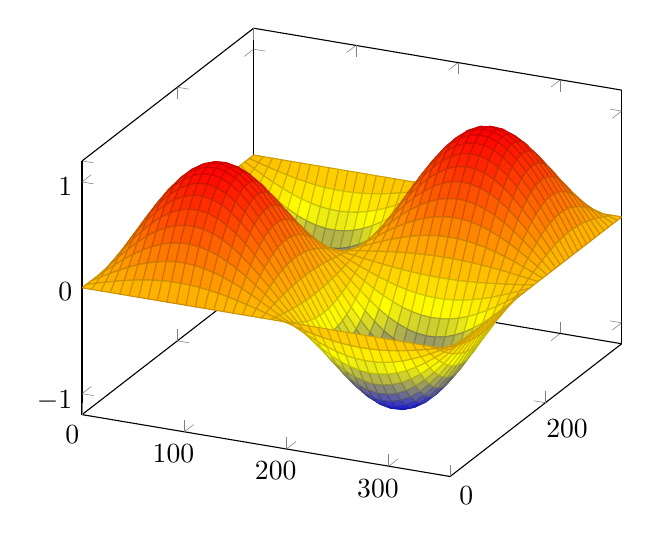
\begin{tikzpicture}
\begin{axis}
\addplot3[
surf,
domain=0:360,
samples=40,
] {sin(x)*sin(y)};
\end{axis}
\end{tikzpicture}
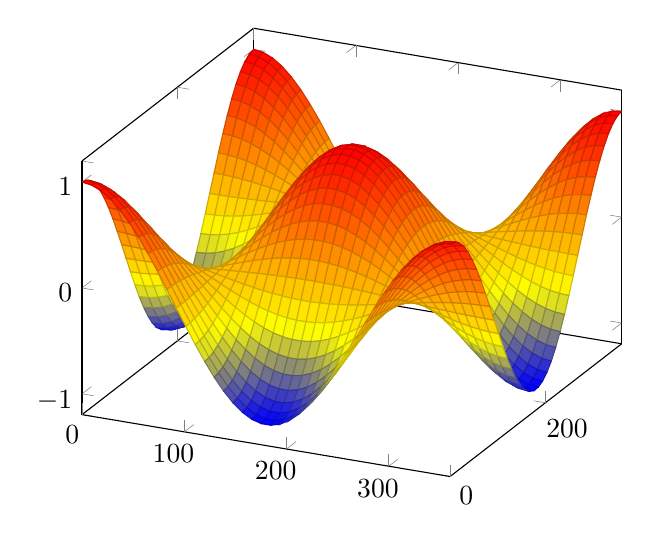
\begin{tikzpicture}
\begin{axis}
\addplot3[
surf,
domain=0:360,
samples=40,
] {cos(x)*cos(y)};
\end{axis}
\end{tikzpicture}

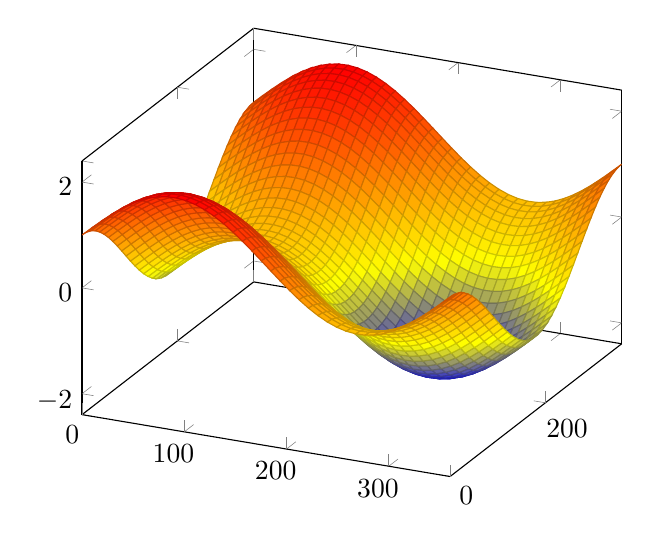
\begin{tikzpicture}
\begin{axis}
\addplot3[
surf,
domain=0:360,
samples=40,
] {sin(x)+cos(y)};
\end{axis}
\end{tikzpicture}
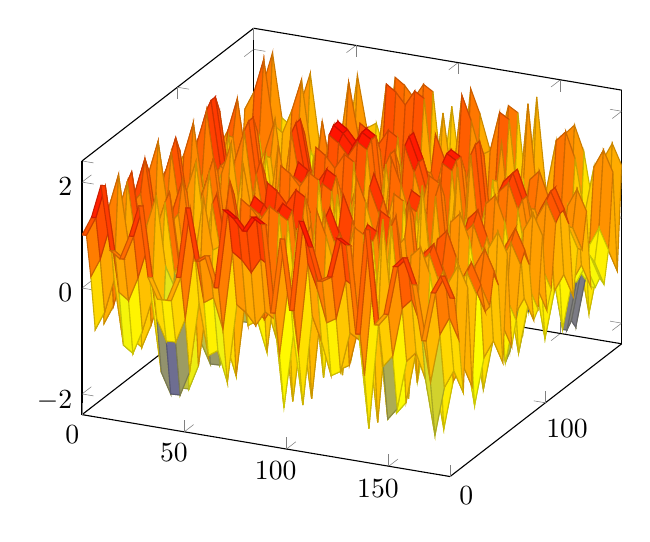
\begin{tikzpicture}
\begin{axis}
\addplot3[
surf,
domain=0:180,
samples=40,
] {sin(x*x)+cos(y*y)};
\end{axis}
\end{tikzpicture}

\begin{tikzpicture}
\begin{axis}
\addplot gnuplot [
id=sin,
] {sin(x)};
\end{axis}
\end{tikzpicture}


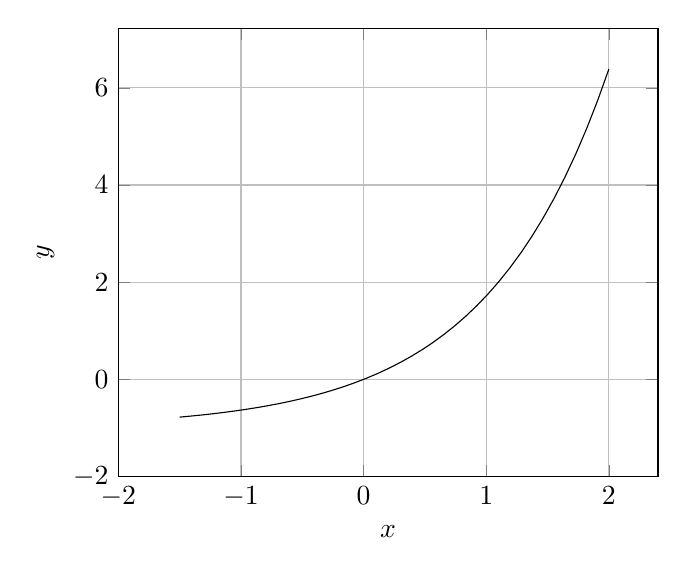
\begin{tikzpicture}
\begin{axis}[
xmin=-2,
ymin=-2,
xlabel= $x$,
ylabel= $y$,
grid=major,
]
\addplot[
domain=-1.5:2,
samples=40,
] {e^x-1};
\end{axis}
\end{tikzpicture}

\begin{tikzpicture}
\begin{axis}[
axis line=center,
xmin=-5.5,
ymin=-4,
xlabel= $x$,x label style={right},
ylabel= $y$,y label style= {above},
grid=major,
]
\addplot[
domain=-5.5:3,
samples=100,
] {1+x+x^2/2+x^3/6+x^4/24};
\end{axis}
\end{tikzpicture}


\begin{tikzpicture}
\datavisualization [school book axes, visualize as smooth line]
data [format=function] {
var x : interval [-1.3:1.3];
func y = \value x*\value x*\value x;
};
\end{tikzpicture}


\section{Symbols, Shortcuts and Semantic Aliasing}

Although Journals recommend not to alias LaTeX commands the harsh reality is that each topic and paper has different needs for notations and things can get messy.

Consider papers written for computations of floating algorithms. We might find in preambles definitions like, 
{\parskip0pt\large
\begin{verbatim}
%% Floating-point machine operations.
\newcommand{\mop}{\boxcircle}
\newcommand{\madd}{\boxplus}
\newcommand{\msub}{\boxminus}
\newcommand{\mmul}{\boxdot}
\newcommand{\mdiv}{\boxdiag}
\end{verbatim}
}
\newcommand{\mop}{\boxcircle}
\newcommand{\madd}{\boxplus}
\newcommand{\msub}{\boxminus}
\newcommand{\mmul}{\boxdot}
\newcommand{\mdiv}{\boxdiag}

I consider aliasing of non-semantic commands to semantic commands, such as the machine operation |\mop| from |\boxcircle| as good practice. 

\begin{texexample}{Example with macro aliasing}{ex;aliasing}
\begin{Definition} \summary{(Absorption.)}
Let $x, y, z \in \Fset$ with $y, z \in \Rset$,
let $\mathord{\mop}$ be any IEEE~754 floating-point operator,
and let $x = y \mop z$.
Then $y \mop z$ gives rise to \emph{absorption} if
\begin{itemize}
\item
$\mathord{\mop} = \mathord{\madd}$
and either $x = y$ and $z \neq 0$, or $x = z$ and $y \neq 0$;
\item
$\mathord{\mop} = \mathord{\msub}$
and either $x = y$ and $z \neq 0$, or $x = -z$ and $y \neq 0$;
\item
$\mathord{\mop} = \mathord{\mmul}$
and either $x = \pm y$ and $z \neq \pm 1$, or $x = \pm z$ and $y \neq \pm 1$;
\item
$\mathord{\mop} = \mathord{\mdiv}$,
$x = \pm y$ and $z \neq \pm 1$.
\end{itemize}
\end{Definition}
\end{texexample}


The most obvious shortcuts should be for calligraphic or fraktur math alphabets.


\begin{texexample}{Calligraphic Alphabet}{ex:callalphabet}
\providecommand*{\cA}{\ensuremath{\mathcal{A}}}
\providecommand*{\cB}{\ensuremath{\mathcal{B}}}
\providecommand*{\cC}{\ensuremath{\mathcal{C}}}
\providecommand*{\cD}{\ensuremath{\mathcal{D}}}
\providecommand*{\cE}{\ensuremath{\mathcal{E}}}
\providecommand*{\cF}{\ensuremath{\mathcal{F}}}
\providecommand*{\cG}{\ensuremath{\mathcal{G}}}
\providecommand*{\cH}{\ensuremath{\mathcal{H}}}
\providecommand*{\cI}{\ensuremath{\mathcal{I}}}
\providecommand*{\cJ}{\ensuremath{\mathcal{J}}}
\providecommand*{\cK}{\ensuremath{\mathcal{K}}}
\providecommand*{\cL}{\ensuremath{\mathcal{L}}}
\providecommand*{\cM}{\ensuremath{\mathcal{M}}}
\providecommand*{\cN}{\ensuremath{\mathcal{N}}}
\providecommand*{\cO}{\ensuremath{\mathcal{O}}}
\providecommand*{\cP}{\ensuremath{\mathcal{P}}}
\providecommand*{\cQ}{\ensuremath{\mathcal{Q}}}
\providecommand*{\cR}{\ensuremath{\mathcal{R}}}
\providecommand*{\cS}{\ensuremath{\mathcal{S}}}
\providecommand*{\cT}{\ensuremath{\mathcal{T}}}
\providecommand*{\cU}{\ensuremath{\mathcal{U}}}
\providecommand*{\cV}{\ensuremath{\mathcal{V}}}
\providecommand*{\cW}{\ensuremath{\mathcal{W}}}
\providecommand*{\cX}{\ensuremath{\mathcal{X}}}
\providecommand*{\cY}{\ensuremath{\mathcal{Y}}}
\providecommand*{\cZ}{\ensuremath{\mathcal{Z}}}
\begin{luacode}
local alphabet = {"A","B","C","D","E","F","G","H","I","J","K","L",
                  "M","N","O","P","Q","R","S","T","U",
                  "V","W","X","Y","Z"}
for k,v in pairs(alphabet) do
	tex.print("\\c"..v..", ")
end
\end{luacode}
\end{texexample}


\section{Calculus}



\subsection*{Differentiation}
Leibnitz invented the transmutation theorem for finding the area under a curve. Finding areas beneath curves
was 


\subsection*{Integration}

\subsection*{Limits}

\marginpar{\includegraphics[width=3cm]{bolzano}
{\scriptsize\RaggedLeft Bolzano begins his work by explaining what he means by theory of science, and the relation between our knowledge, truths and sciences. Human knowledge, he states, is made of all truths (or true propositions) that men know or have known. This is, however, only a very small fraction of all the truths that exist, although still too much for one human being to comprehend. Therefore, our knowledge is divided into more accessible parts. Such a collection of truths is what Bolzano calls a science (Wissenschaft). It is important to note that not all true propositions of a science have to be known to men; hence, this is how we can make discoveries in a science.}}

\textbf{Bolzano} Although implicit in the development of calculus of the 17th and 18th centuries, the modern idea of the limit of a function goes back to Bolzano who, in 1817, introduced the basics of the epsilon-delta technique to define continuous functions. However, his work was not known during his lifetime.\footcite{coolidge} The first publication in English had to wait for almost 150 years and it was published by Coolidge in 1949 in his popular work \emph{The Mathematetics of Great Amateurs.} Grattan-Guiness\footcite{grattan-guiness} falls short though of accusing Cauchy of plagiarizing the work of Bolzano and other contemporaries.


\textbf{Cauchy} discussed variable quantities, infinitesimals, and limits and defined continuity of {$\displaystyle y=f(x)$} $y=f(x)$ by saying that an infinitesimal change in $x$ necessarily produces an infinitesimal change in $y$ in his 1821 book \emph{Cours d'analyse}, while (Grabiner 1983) claims that he only gave a verbal definition. 

\textbf{Weierstrass} first introduced the epsilon-delta definition of limit in the form it is usually written today. He also introduced the notations $\lim$ and $\lim x\rightarrow x_0$. The notation which has been used widely at the time in Europe was
$\operatorname{Lim}_{x=a}$, to express the \enquote{the limit as $x$ approaches $a$.} It is found in papers of Weierstrass, who in 1841 wrote $\lim$ and in 1854 \enquote{$\underset{n=\infty}{\operatorname{Lim.}}\:p_n = \infty $}

In later publications we find $\operatorname{Lim}$ without the point, but still capitalized. I particularly like the way the equations were grouped and the limit indicated by cases and shown in fig.~\ref{weis}.

\begin{figure}[htbp]
\centering
\includegraphics[width=0.8\textwidth]{weistrass}
\caption{Extract from Weierstrass publication.}
\label{weis}

\end{figure}

To create a new operator symbol we can use \cs{operatorname}. The command will take care of spacing, whereas if we use only
|\mathrm| it will not. If we were to use it frequently we could also define a macro using \cs{DeclareMathOperator} from amsmath. 

\begin{texexample}{operatorname}{ex:onames}

$$\operatorname{Lim.}p_n$$

$$\operatorname{Lim}.p_n$$

$$\mathrm{Lim.}p_n$$ 
\end{texexample}

By the early 1900's the notation started approaching more to what is commonly used in today's publications.

\textbf{Hardy} The modern notation of placing the arrow below the limit symbol is due to Hardy in his book \emph{A Course of Pure Mathematics} in 1908, however in the preface to the book he credits Leathem and Bromwich\footcite{bromwich}.\footnote{Hardy wrote ... there are two respects in which I have diverted ...} 


\begin{gather}
\begin{aligned}
f(a) &= f\left[\lim_{k\rightarrow\infty} x_k \right]=\lim_{k} f(x_k)\le 0 & \text{ and }\\
f(a) &= f\left[\lim_{k\rightarrow\infty} X_k \right]=\lim_{k} f(X_k)\ge 0. & \\  
\end{aligned}
\end{gather}

In Cauchy's words, these inequalities established that ``the quantity
$f(a)$ \ldots cannot differ from zero.'' He had thus proved the existence of a
number a between $x$ and $X$ for which $f(a) = O$. The general version of the
intermediate value theorem, namely that a continuous function takes all
values between $f(x_0)$ and $f(X)$, follows as an easy corollary.
This was a remarkable achievement. Cauchy had, for the most part,
succeeded in demonstrating a "self-evident" principle by analytic methods.


Apart from open intervals, limits can be defined for functions on arbitrary subsets of R, as follows.  Let $f$ be a real-valued function defined on a subset $S$ of the real line.  Let $p$ be a limit point of ''S'' that is, ''p'' is the limit of some sequence of elements of ''S'' distinct from p.  The limit of ''f'', as ''x'' approaches ''p'' from values in ''S'', is ''L'' if, for every {{nowrap|''ε'' > ''0''}}, there exists a δ > ''0'' such that {{nowrap|0 < {{abs|''x'' − ''p''}} < ''δ''}} and {{nowrap|''x'' ∈ ''S''}} implies {{nowrap|{{abs|''f''(''x'') − ''L''}} < $\epsilon$.

This limit is often written

\[
L = \underset{x\in S}{\lim_{x\to p}} f(x).
\]

The condition that $f$ be defined on $S$ is that $S$ be a subset of the domain of $f$.  This generalization includes as special cases limits on an interval, as well as left-handed limits of real-valued functions (e.g., by taking ''S'' to be an open interval of the form $(-\infty,a)$, and right-handed limits (e.g., by taking ''S'' to be an open interval of the form $(a,\infty)$. It also extends the notion of one-sided limits to the included endpoints of (half-)closed intervals, so the Square root function $f(x)=\sqrt{x}$ can have limit 0 as $x$ approaches 0 from above.




\section*{Fraktur letters}

Individual Fraktur letters are sometimes used in mathematics, which often denotes associated or parallel concepts by the same letter in different fonts. For example, a Lie group is often denoted by ''G'', while its associated Lie algebra is $\mathfrak{g}$. 
A ring ideal might be denoted by $\mathfrak{a}$ (or $\mathfrak{p}$ if a prime ideal) while an element is $a \in \mathfrak{a}$. The Fraktur $\mathfrak c$ is also sometimes used to denote the cardinality of the continuum, that is, the cardinality of the real line. In model theory, $\mathfrak{A}$ is used to denote an arbitrary model, with ''A'' as its universe. Fraktur is also used in other ways at the discretion of the author.


\begin{luacode}
local alphabet = {"A","B","C","D","E","F","G","H","I","J","K","L",
                  "M","N","O","P","Q","R","S","T","U","V","W","X","Y","Z"}
for k,v in pairs(alphabet) do
	tex.print("\\mathfrak{"..v.."}, ")
end
\end{luacode}

Special symbols such as dingbats loaded using the \pkg{pifont} package need to be enclosed within an \docAuxCommand{mbox} in order to be able to display the glyph properly.
\bigskip

\begin{texexample}{Using special dingbat symbols}{}
\label{e14}
 We start by showing that the function $f(x)=x^2$ is
continuous over the set $X_2$\label{p:X2} defined as the interval
$[0,1]$ where numerals $\frac{i}{\mbox{\ding{172}}}, 0 \le i \le
\mbox{\ding{172}},$ are used to express its points in units $\mu$.
First of all, note that the set $X_2$ is continuous in   $\mu$
because its points are equidistant with the distance
$d=\mbox{\ding{172}}^{-1}$. Since this function is strictly
increasing,  to show its continuity it is sufficient to check the
difference $f(x)-f(x^{-})$ at the point $x=1$. In this case,
$x^{-}=1-\mbox{\ding{172}}^{-1}$ and we have
\[
 f(1)-f(1-\mbox{\ding{172}}^{-1})=
 1-(1-\mbox{\ding{172}}^{-1})^2 =
 2\mbox{\ding{172}}^{-1}(-1)\mbox{\ding{172}}^{-2}.
\]
This number is infinitesimal, thus $f(x)=x^2$ is continuous over
the set $X_2$. \hfill $\Box$
\end{texexample}

\cs{Box}
Notice the use of the \docAuxCommand{Box} command to draw a square for  end of proof symbol. This is from the amsmath package. The box is placed at the end of the line using |\hfill $\Box$|.

%
%\begin{Rule}
%Alias common symbols to semantic macro names that follow their mathematical definitions.
%\end{Rule}
%
%\begin{Rule}
%Create shorcut commands with moderation for alphabets and algebras and alias if necessary. Good practice, sets etc.
%\end{Rule}



\section{Partial derivatives}

Partial derivatives can be typeset using the \latex{} command \cs{partial}

\begin{texexample}{Partial Derivatives}{ex:partial}
\[
dS = \frac{\partial S}{\partial x}\, dx
   + \frac{\partial S}{\partial y}\, dy
   = \left(y - \frac{2V}{x^2}\right) dx
   + \left(x - \frac{2V}{y^2}\right) dy.
\]
\meaning\partial
\end{texexample}


This is using a certain style. For other styles it maybe more difficult.

\section*{Binomial Coefficients}

To typeset binomial coefficients or similar structures, use the command
\cs{binom} from \pkg{amsmath}\index{amsmath>binom}

\begin{texexample}{Binomial}{ex:binomial0}
\[
\begin{align}
(x+y)^3 & = x^3 + 3x^2y + 3xy^2 + y^3, \\[8pt]
(x+y)^4 & = x^4 + 4x^3y + 6x^2y^2 + 4xy^3 + y^4, \\[8pt]
(x+y)^5 & = x^5 + 5x^4y + 10x^3y^2 + 10x^2y^3 + 5xy^4 + y^5, \\[8pt]
(x+y)^6 & = x^6 + 6x^5y + 15x^4y^2 + 20x^3y^3 + 15x^2y^4 + 6xy^5 + y^6, \\[8pt]
(x+y)^7 & = x^7 + 7x^6y + 21x^5y^2 + 35x^4y^3 + 35x^3y^4 + 21x^2y^5 + 7xy^6 + y^7.
\end{align}
\]
\end{texexample}


Pascal's rule can be typeset as:


\begin{texexample}{Binomial Distribution}{ex:binomial}
\[
\binom{n}{k} =\binom{n-1}{k}
+ \binom{n-1}{k-1}
\]
\end{texexample}



\section[Symbols and Abbreviations]{Symbols and Abreviations}
\label{math:abbreviations}

\label{abbr}\label{symbols}%

\begin{texexample}{Creating symbols}{ex:parallelogram}
\newlength{\dentwidth}\setlength{\dentwidth}{\textwidth}
\addtolength{\dentwidth}{-\parindent}

\makeatletter
\gdef\@parallelogram#1{%
  \textnormal{\setbox\z@\hbox{#1/}\dimen@\wd\z@
   \@tempdima 2.45\dimen@
   \vbox{\offinterlineskip
      \hbox{\kern.8\dimen@\vrule\@width\@tempdima\@height.4\p@}%
      \kern-.0\p@
      \hbox to\@tempdima{#1/\hfil\rlap/}%
      \kern-.5\p@
      \hbox{\kern.1\dimen@\vrule\@width\@tempdima\@height.4\p@}}}}
      
 \gdef\Par{%
   \mathchoice
      {\@parallelogram\scriptsize}%
      {\@parallelogram\scriptsize}%
      {\@parallelogram\tiny}%
      {\@parallelogram\tiny}}

            



\begin{tabular*}{\dentwidth}{rl@{\extracolsep{\fill}}l@{\extracolsep{0pt}}@{\dots}l}

$>$ & is (or are) greater than. & Def. & definition. \\
$<$ & is (or are) less than. & Ax. & axiom. \\
$\Bumpeq$ & is (or are) equivalent to. & Hyp. & hypothesis. \\
$\therefore$ & therefore. & Cor. & corollary. \\
$\perp$ & perpendicular. & Scho. & scholium. \\
$\perp_s$ & perpendiculars. & Ex. & exercise. \\
$\parallel$ & parallel.\qquad $\parallel_s$ parallels. & Adj. & adjacent. \\
$\angle$ & angle.\qquad $\angle_s$ angles. & Iden. & identical. \\
$\triangle$ & triangle.\qquad $\triangle_s$ triangles. & Const. & construction. \\
$\Par$ & parallelogram. & Sup. & supplementary. \\
$\Par_s$ & parallelograms. & Ext. & exterior. \\
$\odot$ & circle.\qquad $\odot_s$ circles. & Int. & interior. \\
rt. & right.\qquad  st.\ straight. & Alt. & alternate. \\
\end{tabular*}


\hbox{\qed\ stands for quod erat demonstrandum, \emph{which was to be proved}.\hss}

\newcommand{\qef}{\textsc{q.e.f.}}
\qef\ stands for quod erat faciendum, \emph{which was to be done.}

The signs $+$, $-$, $\times$, $\div$, $=$, have the same meaning as in Algebra.

\makeatother   
\end{texexample}
   
\section{Afixing symbols to other symbols}

\latex provides \docAuxCommand{stackrel} for placing a superscript above a binary relation. In the \pkg{amsmath} package there are somewhat more general commands \docAuxCommand{overset} and \docAuxCommand{underset}, that can be used to place one symbol above or below another symbol, whether is a relation or something else. Oberdiek's package \pkg{stackrel}\footcite{stackrel} extends the syntax by adding an optional argument for the subscript position. It follows the syntax of extensible arrows of the packages |amsmath| and |mathtools|.

\begin{docCommand}{stackrel}{\oarg{subscript}\marg{superscript}{\marg{rel}}}
  Typeset a subscript or superscript above a symbol.
\end{docCommand}

\ifSTACKREL
\begin{texexample}{Example of stackrel and stackbin}{ex:stackrel}
\[
 A \stackbin[\text{and}]{}{+} B \stackrel[x]{!}{=} C
\] 
\end{texexample}
\else
\begin{texcode}{Example of \cs{stackrel} and \cs{stackbin}}{ex:stackrel}
  Example cannot be shown as the package stackrel is not loaded.
\end{texcode}
\fi


\chapter{Matrices and Mathematical Environments}
\label{matrices}

\section{Matrices}

Matrices have a long history of application in solving linear equations but they were known as arrays until the 1800s. The Chinese text The Nine Chapters on the Mathematical Art written in 10th–2nd century BCE is the first example of the use of array methods to solve simultaneous equations,[102] including the concept of determinants. In 1545 Italian mathematician Gerolamo Cardano brought the method to Europe when he published Ars Magna.[103] The Japanese mathematician Seki used the same array methods to solve simultaneous equations in 1683.[104] 


The Dutch statesman and mathematician Johan (Jan) de Witt represented transformations resembling arrays in his 1659 book Elements of Curves (1659). He is also perhaps the second Mathematician to be lynched\footnote{Hypatia, was torn to bits by a lynching Christian mob in the streets of Alexandria in \textsc{AD} 415.} by a mob and had parts of their bodies eaten! [\ldots]The brothers were shot and then left to the mob. Their naked, mutilated bodies were strung up on the nearby public gibbet, while the Orangist mob partook of their roasted livers in a cannibalistic frenzy. Throughout it all, a remarkable discipline was maintained by the mob, according to contemporary observers, making one doubt the spontaneity of the event.\footcite{israel1995} \textit{Elementa Curvarum Linearum} has been described as the first textbook in analytic geometry.\footnote{The savage murder of a man that history has judged a highly competent leader is regarded by the Dutch as one of the most shameful episodes in their history.}


Between 1700 and 1710 Gottfried Wilhelm Leibniz publicized the use of arrays for recording information or solutions and experimented with over 50 different systems of arrays.[103] Cramer presented his rule in 1750.

The term "matrix" (Latin for "womb", derived from mater—mother[106]) was coined by James Joseph Sylvester in 1850,[107] who understood a matrix as an object giving rise to a number of determinants today called minors, that is to say, determinants of smaller matrices that derive from the original one by removing columns and rows. In an 1851 paper, Sylvester explains:

\begin{quote}
I have in previous papers defined a \enquote{Matrix} as a rectangular array of terms, out of which different systems of determinants may be engendered as from the womb of a common parent.[108]
\end{quote}

Arthur Cayley published a treatise on geometric transformations using matrices that were not rotated versions of the coefficients being investigated as had previously been done. Instead he defined operations such as addition, subtraction, multiplication, and division as transformations of those matrices and showed the associative and distributive properties held true. Cayley investigated and demonstrated the non-commutative property of matrix multiplication as well as the commutative property of matrix addition.[103] Early matrix theory had limited the use of arrays almost exclusively to determinants and Arthur Cayley's abstract matrix operations were revolutionary. He was instrumental in proposing a matrix concept independent of equation systems. In 1858 Cayley published his A memoir on the theory of matrices[109][110] in which he proposed and demonstrated the Cayley–Hamilton theorem.[103] Cayley introduced a particular notation for fencing the array as shown in fig~\ref{fig:cayley}, which used () for the first row and $\vert$ for subsequent rows.

\begin{figure}[htbp]
\centering
\includegraphics[width=0.6\textwidth]{cayley-notation}

\caption{Extract from Caley's paper \textit{A memoir on the theory of matrices.}}
\label{fig:cayley}

\end{figure}

An English mathematician named Cullis was the first to use modern bracket notation for matrices in 1913 and he simultaneously demonstrated the first significant use of the notation $A = [a_{i,j}]$ to represent a matrix where $a_{i,j}$ refers to the i$^$th row and the $j$th column.

Cayley's introductory paper in matrix theory was written in French and published in a German periodical. In this paper, matrices are introduced to simplify the notation which arises in simultaneous linear equations.  

\begin{gather}
\begin{aligned}
\xi  &= \alpha x + \beta y + \gamma z + \dots\\
\eta  &= \alpha' x + \beta' y + \gamma' z + \dots\\
\zeta &= \alpha'' x + \beta'' y + \gamma'' z + \dots
\end{aligned}
\end{gather}

The set of equations is written as:

\begin{gather}
(\xi, \eta, \zeta,\dots ) = (\alpha,\beta,\gamma,\dots)(x,y,z,\dots)
\end{gather}

The same article also introduces, although quite sketchily, the ideas of inverse matrix and of matrix multiplication, or \enquote{compounding} as Cayley called it. The above basic properties are expanded in a second expository article\footcite{fieldman1962} which
also lists many additional properties of matrices. In this important paper, Cayley works mostly with square matrices with
nine elements. He represents the zero matrix,\footcite[This is an interesting development]{fieldman1962}

\[
\begin{vmatrix}
0,0,0\\
0,0,0\\
0,0,0
\end{vmatrix}
\]
by \enquote{0} and the \enquote{matrix unity,}

\[
\begin{vmatrix}
1,0,0\\
0,1,0\\
0,0,1
\end{vmatrix}
\]
by \enquote{1}

Caley then introduces the algebra of matrices by defining the addition of two matrices by

\begin{gather}
(\begin{cayleymatrix}{3}
a&b&c\\
a' &b' & c'\\
a''&b'' & c''\\
a''' & b''' & c'''\\
\end{cayleymatrix}) +
(\begin{cayleymatrix}{3}
\alpha & \beta & \gamma\\
\alpha & \beta & \gamma\\
\alpha & \beta & \gamma\\
\end{cayleymatrix})\:\: = \:\:
(\begin{cayleymatrix}{3}
a+a  &b+b  &c+\gamma\\
a''+\alpha' & b'' + \beta'' & c'' +\gamma'' \\
a'''+\alpha''' & b''' + \beta''' & c''' +\gamma''' \\
\end{cayleymatrix})
\end{gather}
Caley stated but without proof, that matrices are commutative and associative under addition. Two types
of multiplication are exhibited. The first type is designated as \enquote{scalar multiplication,} that is

\[
m(\begin{cayleymatrix}{3}
a & b & c\\
a' & b' & c'\\
a'' & b'' & c''
\end{cayleymatrix}) 
= 
(\begin{cayleymatrix}{3}
ma & mb & mc\\
ma' & mb' & mc'\\
ma'' & mb'' & mc''
\end{cayleymatrix})
\]

The notation used for the matrix (\begin{cayleymatrix}{3}
a&b\\
c&d\\
e&f
\end{cayleymatrix}) is defined later on. It is a special environment.

The second type of multiplication is called \enquote{compounding,} according to the following scheme:

\begin{multline}
(\begin{cayleymatrix}{3}
a  &b &c\\
a' &b' &c'\\
a'' &b'' &c''
\end{cayleymatrix}\between \begin{cayleymatrix}{3}
\alpha & \beta & \gamma\\
\alpha'' & \beta'' & \gamma''\\
\alpha'' & \beta'' & \gamma''\\
\end{cayleymatrix})
\\=
 (\begin{cayleymatrix}{3} \bigl(a,b,c\between a, a',a''\bigr) & (a,b,c\between (\beta, \beta', \beta'') & (a,b,c\between \gamma, \gamma', \gamma'')\\
(a &b &c\\
(a &b &c
\end{cayleymatrix})\label{caleyprod}
\end{multline}

The product equation is complex to type, but very clear to understand its definition.\footnote{Uses multline environment.}


Later developments are described by Feldmann\footcite[This is the second paper that appeared in the \textit{The Mathematics Teacher relating to matrices.}][]{feldmann1963}. 

In the 1930s books on matrices written in English started to appear. The two leading ones were C.C. MacDuffee \textit{Theory of Matrices,} Springer (1933) and J. H. M. Wedderburn \textit{Lectures on Matrices}\footnote{The book was published by the American Mathematical Society and bears reseblance to a publication printed using TeX.} (1934). They both wrote matrices with double vertical lines as in

\[
\begin{Vmatrix}
a_{11} & a_{12} & \dots & a_{1n}\\
a_{11} & a_{12} & \dots & a_{1n}\\
\vdots & \vdots & \vdots & \vdots\\
a_{n1} & a_{n2} & \dots &a_{nn}
\end{Vmatrix}
\]
The use of double vertical lines was easy to typeset as well as to handwrite. It could also relate to the single vertical lines which are used to denote determinants.




%%%%%%%%%%%%%%%%%%%%%%%%%%%%%%%%%%%%%%%%%%%%%
%%%%%%%%  TYPOGRAPHY %%%%%%%%%%%%%%%%%%%%%%%%
\section{Typography of Matrices}

Matrices are mostly typed the way tabular environements are types, i.e., you need to use the tabulator sign ``\&''.
Mathematical environments are provided both by \latexe as well as amsmath. The latter are to be preferred.

\begin{docEnvironment}{array}{\marg{specifier}}
\end{docEnvironment}

The |array| environment is a \latex2e provided environment and is identical to tabular, but works automatically with mathematics. It has to be enclosed in a mathematical environment.


\begin{texexample}{Matrices}{ex:matrices}
\[
\mathbf{X} = \left(
\begin{array}{ccc}
x_1 & x_2 & \ldots \\
x_3 & x_4 & \ldots \\
\vdots & \vdots & \ddots
\end{array} \right)
\]
\end{texexample}

\section{AMS Math matrices}

The \pkg{amsmath} package provides environments that go beyond the basic \docAuxEnvironment{array} of \latex2e. The \docAuxEnvironment{pmatrix}, \docAuxEnvironment{Bmatrix}, \docAuxEnvironment{vmatrix} and \docAuxEnvironment{Vmatrix}. 
There is also a \docAuxEnvironment{smallmatrix} that is more suitable for inline text display. 

\begin{texexample}{Using \textbackslash smallmatrix}{ex:smallmatrix}
This is a small matrix $\bigl(\begin{smallmatrix}
a&b\\
c&d\\
\end{smallmatrix}\bigr)$ environment. \lorem
\end{texexample}


\begin{docEnvironment}{bmatrix}{}
The example \ref{ex:bmatrix} illustrates the typesetting of a bracketted matrix hence \ul{b}matrix. If you want the matrix equation to be numbered enclose it withn an |equation| or |gather| environment. In this documentation we have let the |equation| environment to |gather| hence it will make no difference which ever is used. (amsmath)
\end{docEnvironment}

\begin{texexample}{Bmatrix}{ex:bmatrix}
\begin{equation}
\begin{matrix}
1 & 2 \\
3 & 4
\end{matrix} \qquad
\begin{bmatrix}
p_{11} & p_{12} & \ldots & p_{1n} \\
p_{21} & p_{22} & \ldots & p_{2n} \\
\vdots & \vdots & \ddots & \vdots \\
p_{m1} & p_{m2} & \ldots & p_{mn}
\end{bmatrix}
\end{equation}
\end{texexample}

The \refEnv{bmatrix} is from the amsmath package, see also \vref{bmatrix} and \nameref{bmatrix} and \pageref{bmatrix}. 


One issue to be aware is that the \refEnv{bmatrix} does not allow more than 10 tab stops. If you need to use more, you will have to \docCounter{MaxMatrixCols} to a higher number. The |phd| package sets this automatically at 20, so you will not have to worry about it.

\begin{teX}
\setcounter{MaxMatrixCols}{20}
\end{teX}

\begin{texexample}{Large Matrices}{ex:largematrices}
\[
\begin{bmatrix}
1 & 0 & 0 & -1 & 0  & 0  & 1 & -1 & 1  & -1 & 0 \\
0 & 1 & 0 & 0  & -1 & 0  & 1 & -1 & 0  & 1  & -1 \\
0 & 0 & 1 & 0  & 0  & -1 & 1 & -1 & -1 & 0  & 1 
\end{bmatrix}
\]
\end{texexample}



\section{vmatrix}

\begin{texexample}{vmatrix}{ex:vmatrix}

\begin{gather}
\begin{vmatrix}
aa' + bb' + cc' & ea' + fb' + gc' \\
ae' + bf' + cg' & ee' + ff' + gg'
\end{vmatrix}
{} = \begin{vmatrix}
a & b \\
e & f
\end{vmatrix}  \begin{vmatrix}
a' & b' \\
e' & f'
\end{vmatrix} + \begin{vmatrix}
a & c \\
e & g
\end{vmatrix}  \begin{vmatrix}
a' & c' \\
e' & g'
\end{vmatrix}.
\end{gather}
\end{texexample}





\section{Single equations that are too long}

In many cases equations need to be written over two or more lines. The \pkgname{amsmath} package, provides environments that are suitable for this:


\begin{texexample}{The multiline amsmath environment}{ex:multiline}
\begin{multline}
   a + b + c + d + e + f+ g + h + i  + k + l + m + n + o + p\\
              = j + k + l + m + n +\cos^{2}-1
\end{multline}
\end{texexample}



\section{array environment}

This is simply the same as the |eqnarray| environment only with the possibility of
variable rows and columns and the fact, that the whole formula has only one
equation number and that the array environment can only be part of another math
environment, like the equation environment or the displaymath environment. With
@{} before the first and after the last column the additional space |\arraycolsep| is
not used, which maybe important when using left aligned equations.

\begin{texexample}{array environment}{ex:array2}
\begin{eqnarray}
  a & = & b + c \\
    & = & d + e + f + g + h + i
               + j + k + l \nonumber \\
    &   & +\: m + n + o \\
    & = & p + q + r + s
\end{eqnarray}
\end{texexample}

The equations
to be aligned are entered with each one terminated by \cs{cr}. In each equation there should be
one alignment symbol \& to indicate where the alignment should take place. This is usually
done at the equal signs, although it is not necessary to do so. For example


\begin{texexample}{The array environment}{ex:array}
Thus to change $\frac34$ to a decimal divide $4$ into $3$
and we get $.75$ as a result, thus:
\[
\begin{array}{r@{}r@{}}
4 \; & \vline \; 3.00 \\\cline{2-2}
     &            .75
\end{array}
\]

To find the square root of a four-figure number
such as our example calls for, work it out in the
following manner:
\[
\arraycolsep=0em
\begin{array}{cccccccccccc}
\multicolumn{3}{c}{\text{2d pair}} &\qquad&\qquad&
\multicolumn{3}{c}{\text{1st pair}}&\qquad&\qquad&
\multicolumn{2}{c}{\text{square root}}\\
 & \overbrace{\quad}&\ZZZ&&&\ZZZ&\overbrace{\quad}&\ZZZ\\
 & 42 &&&&& 25 &&&&\vline\;65&(answer)\\\cline{11-11}
 & 36 &&&&& \\\cline{2-2}
\multirow{2}{*}{125\:} & \vline\hfill \Zi6 \hfill&&&&& 25\\
 & \vline\hfill \Zi6 \hfill&&&&& 25\\\cline{2-7}
\end{array}
\]
\end{texexample}


\subsection{Array environment in game theory}

This example \ref{ex:gamearray} is from \footnote{From determinacy to Nash equilibrium,St\'ephane Le Roux, TU Darmstadt }

\begin{texexample}{array environment in game theory}{ex:gamearray}
The game $\langle\{a,b,c\},\{1,2,3,4\}^3,\{0,1,2,3,4\},v,(<_d)_{d\in\{a,b,c\}}
\rangle$ is represented below, where player $a$ chooses the row, $b$ the column, and $c$ the array. 
\[\begin{array}{c@{\hspace{1cm}}c@{\hspace{1cm}}c@{\hspace{1cm}}c}
\begin{array}{|c|c|c|c|}
\hline 1 & 1 & 1 & 1\\
\hline 1 & 1 & 1 & 1\\
\hline 1 & 1 & 1 & 1\\
\hline 4 & 1 & 1 & 1\\
\hline
\end{array}
&
\begin{array}{|c|c|c|c|}
\hline 1 & 2 & 1 & 1\\
\hline 2 & 2 & 2 & 2\\
\hline 1 & 2 & 1 & 1\\
\hline 4 & 2 & 1 & 1\\
\hline
\end{array}
&
\begin{array}{|c|c|c|c|}
\hline 1 & 1 & 3 & 1\\
\hline 1 & 1 & 3 & 1\\
\hline 3 & 3 & 3 & 3\\
\hline 4 & 1 & 3 & 1\\
\hline
\end{array}
&
\begin{array}{|c|c|c|c|}
\hline 2 & 4 & 4 & 4\\
\hline 4 & 3 & 4 & 4\\
\hline 4 & 4 & 4 & 4\\
\hline 0 & 0 & 0 & 0\\
\hline
\end{array}
\end{array}
\]
Let us show that the game $\langle\{a,b,c\},\{1,\dots,n\}^3,\{0,\dots,n\},v,(<_d)_{d\in\{a,b,c\}}
\rangle$ witnesses the claim. First, the preferences are linear orders indeed. Second, let us show that there is no Nash equilibrium by case-splitting below. 
\end{texexample}



\section{The AMSmath Package}

\index{maths environment>align}
\index{maths environment>align}
\index{maths environments}{falign}
\index{maths environments}{xalignat}
\index{maths environments}{xxalignat}
\index{maths environments}{eqnarray}

The \pkg{amsmath} package offers five different align environments, |align|, |alignat|, |falign|, |xalignat| and |xxalignat|. 

In difference to the \refEnv{eqnarray} environment from standard \latex the ``three'' parts of one equation expr.-symbol-expr. are divided by only one ampersand in two parts. In general the ampersand should be before the symbol to get the right spacing, for example y \&= x. 

\subsection{The align environment}

The |align| environment is considered an improvement over \latex's |eqnarray| environment. It is very similar to a tabular
environment and is aligned at the |&|. 
It requires one |&| less and produces a tighter equation. Mathematicians 
are very particular in not using |eqnarray| and the package 
\pkgname{onlyamsomath} if used will warn if it finds that it has been used in the document. 
\index{eqnarray (environment)>spacing}
\index{eqnarray (environment)>alternatives}
\index{math environments>align}
\index{math environmenta>eqnarray}


\begin{texexample}{Comparison between |align| and |eqnarray|}{ex:eqnarraycomp}
% First example with eqnarray
\begin{eqnarray}
a & = & b + c \\
  & = & d + e + f + g + h + i
        + j + k + l \nonumber \\
  &   & +\: m + n + o \\
  & = & p + q + r + s
\end{eqnarray}

% Second example with align
\begin{align}
a & =  b + c \\
  & =  d + e + f + g + h + i
       + j + k + l \nonumber \\
  & +\: m + n + o \\
  & =  p + q + r + s
\end{align}
\end{texexample}


You can observe in Example~\ref{eqnarraycomp} the essential differences between the two, which we re-iterate, it requires one less |&| and produces a tighter display.

\begin{texexample}{The align environment}{ex:align}
\begin{align}
         y & = d\label{eq:IntoSection}\\
         y & = cx+d\\
    y_{12} & = bx^{2}+cx+d\\
     y(x)  & = ax^{3}+bx^{2}+cx+d
 \end{align}

%\begin{align*}
%\therefore (13 - x_1) + (13 - x_2) + \dotsb + (13 - x_p) + r &= 52\,,\\
%\therefore 13p - (x_1 + x_2 + \dotsb + x_p) + r              &= 52\,,\\
%\therefore x_1 + x_2 + \dotsb + x_p                          &= 13p - 52 + r\\
%                                                          &= 13 (p - 4) + r\,.
%\end{align*}

whence we conclude that $\gamma$ is a primitive root modulo $p$. But
\begin{align*}
\gamma^{p-1}-1 &=
     g^{p-1} - 1 + \frac{p-1}{1!}g^{p-2}xp +
        \frac{(p-1)(p-2)}{2!}g^{p-3}x^2p^2 + \ldots \\
  &= p\left(kp + \frac{p-1}{1!}g^{p-2}x +
        \frac{(p-1)(p-2)}{2!}g^{p-3}x^2p + \ldots\right).
\end{align*}
\end{texexample}

As you can observe from example\ref{ex:align}, each line is numbered if the unstarred version of the command is used. The |aligned| environment remedies this.
 


\subsection{The aligned environment}

The aligned environment allows more than one horizontal alignment but has only one equation number.

%\newcommand{\dotsbsmall}{\ldot\!\ldot\!\ldot}
%\newcommand{\ldot}{\mathbin{.}}			% dot with math spacing
%\newcommand{\nobf}[1]{\no \textbf{#1}}		% no with bold number
%
%\begin{texexample}{aligned environment example}{}
%\begin{equation}
%\begin{aligned}
%  &\:C_1x^{r_1}\,[\varphi_{r_1 0} \,+ \varphi_{r_1 1}\log x \,+ \dotsb + \varphi_{r_1 \alpha_1}(\log x)^{\alpha_1}]\\
%+ &\:C_2x^{r_2}\,[\varphi_{r_2 0} \,+ \varphi_{r_2 1}\log x \,+ \dotsb + \varphi_{r_2 \alpha_2}(\log x)^{\alpha_2}]\\
%+ &\multispan{1}{\:\dotfill}\\
%+ &\:C_nx^{r_n}[\varphi_{r_n 0} + \varphi_{r_n 1}\log x + \dotsb + \varphi_{r_n \alpha_n}(\log x)^{\alpha_n}],
%\end{aligned}
%\end{equation}
%
%\[
%\tag{98}
%\left\{\qquad
%\begin{aligned}
%T_1 &= T_2 = T_3 (=T)\\
%p_1 &= p_2 = p_3\\
%s_1-s_2 &= \frac{(u_1-u_2)+p_1(v_1-v_2)}{T}\\
%s_2-s_3 &= \frac{(u_2-u_3)+p_2(v_2-v_3)}{T}.
%\end{aligned}
%\right.
%\]
%\end{texexample}
 




\subsection{How to interrupt a display}

\begin{docCommand}{intertext}{}
 In many instances you will want to interrupt a display with some text. This can be accomplished using the control sequence |\intertext|.
 \end{docCommand}
 
 

\begin{texexample}{Using \cs{intertext}}{ex:intertext}
\begin{gather}
\begin{aligned}
U &= M u = M(c_v T + b)\\
S &= M(c_v  \log T + \frac{R}{m}  \log v + a),\\
\intertext{and } 
F &= M \left\{T(c_v - a - c_v \log T) - \frac{RT}{m} \log v + b \right\}.
\end{aligned}
\end{gather}
\end{texexample}

As the command \docAuxCommand{intertext} can only come after a |\\|  command we place it accordingly at {1}. Its function is to preserve the alignment after the text is typeset. This is a common requirement in many mathematical 
structures and the command can be used in all of amsmath aligning environments.







\subsection{The alignat environment}

\begin{docEnvironment}{alignat}{}
The alignat environment means \emph{align at} and can be used to align a set of equations vertically at more than one place. The star version of the environment omits the equation numbering.
\end{docEnvironment}


%\begin{texexample}{The alignat environment}{}
%\renewcommand{\dotsb}{\ldots}			% use lower dots after +-
%\renewcommand{\dotsbsmall}{\ldot\!\ldot\!\ldot}
%\renewcommand{\ldot}{\mathbin{.}}			% dot with math spacing
%\renewcommand{\nobf}[1]{\no \textbf{#1}}	
%
%\begin{alignat*}{5}
%  &p_{i+1}\dfrac{d^{m-i-1}y_1}{dx^{m-i-1}} &&+ \dotsbsmall +p_{m}y_1
%  && = -\Big(\dfrac{d^{m}y_1}{dx^{m}} &&+p_1\dfrac{d^{m-1}y_1}{dx^{m-1}}
%  &&+ \dotsbsmall +p_{i}\dfrac{d^{m-i}y_1}{dx^{m-i}}\Big), \\
%\multispan{10}{\makebox[36em]{\dotfill},}\\
% &p_{i+1}\dfrac{d^{m-i-1}y_{m-i}}{dx^{m-i-1}} &&+ \dotsbsmall +p_{m}y_{m-i}\!
% &&= -\Big(\dfrac{d^{m}y_{m-i}}{dx^{m}} &&+ p_1\dfrac{d^{m-1}y_{m-i}}{dx^{m-1}}
% &&+ \dotsbsmall +p_{i}\dfrac{d^{m-i}y_{m-i}}{dx^{m-i}}\Big).
%\end{alignat*}
%\end{texexample}



Remember that when using one of the align environments, there should be no |\\| at the end of the
last line, otherwise you will get another equation number for this ``empty''  line.


\subsection{Multline}

\begin{docEnvironment}{multline}{\meta{contents}}
\end{docEnvironment}
The |multline| environment is another attempt at displaying long equations. It will set the first line flush left and the last one flush right. It can be quite useful when one has very long equations. The line break is marked with |\\|. It is good typographical practice to have the first line shorter than the last line and not the other way around.

\begin{texexample}{Multiline Equations}{mult}
Example unumbered
\begin{multline*}
x^{\rho}f(x, \rho) = x^{\rho} \Big [ u_{m}x^{m}\frac{\rho(\rho-1)\ldots (\rho-m+1)}{x^{m}} \\
                   + u_{m-1}x^{m-1}\frac{\rho(\rho-1)\ldots (\rho-m+2)}{x^{m-1}}+ \ldots
                   + u_{2}x^{2}\frac{\rho(\rho-1)}{x^2}+u_{1}x\frac{\rho}{x}+u_0 \Big ].
\end{multline*}
Example  numbered
\begin{multline}
M \left[\delta u - \left(T_1\, \frac{dp_{12}}{dT_{12}} - p_1\right) \delta v\right] \\
= \delta T_{12} \left[M_{12}\, \frac{du_{12}}{dT_{12}} + M_{21}\, \frac{du_{21}}{dT_{12}}
  - \left(T_1\, \frac{dp_{12}}{dT_{12}} - p_1\right)
    \left(M_{12}\, \frac{dv_{12}}{dT_{12}}
        + M_{21}\, \frac{dv_{21}}{dT_{12}}\right)\right].
\end{multline}
\end{texexample}



\section{gathered}

The |gathered| environment is like the |aligned| or |alignat| environment. They use
only so much horizontal space as the widest line needs. In difference to the gather
environment it must be itself inside math mode.

\begin{docEnvironment}{gathered}{\meta{contents}}
\end{docEnvironment}

\emphasize{cases}
\begin{texexample}{The gathered environment}{exe:gathered}
\[
  \left .
   \begin{gathered}
    \left [ \frac{\alpha}{p} \right ] +
    \left [ \frac{\alpha}{p^2} \right ] +
    \left [ \frac{\alpha}{p^3} \right ] +
    \ldots \\
    \left [ \frac{\beta}{p} \right ] +
    \left [ \frac{\beta}{p^2} \right ] +
    \left [ \frac{\beta}{p^3} \right ] +
    \ldots \\
      \vdots \\
    \left [ \frac{\lambda}{p} \right ] +
    \left [ \frac{\lambda}{p^2} \right ] +
    \left [ \frac{\lambda}{p^3} \right ] +
    \ldots
   \end{gathered}
  \right \} \tag{B}
\]
\end{texexample}

\section{The cases environment}

The \refEnv{cases} environment renders multiple lines with an extensible left curly-brace. It can be used for piecewise-defined functions. For this to work, you must have |\usepackage{amsmath}| in the preamble.

\newlength{\boxla}
\newlength{\boxlb}
\newlength{\boxlc}
\setlength{\boxla}{1.15in}
\setlength{\boxlb}{1.7in}
\setlength{\boxlc}{1.6in}
\newcommand{\boxa}[1]{\makebox[\boxla]{\small #1\dotfill}}
\newcommand{\boxb}[1]{\makebox[\boxlb]{\small #1\dotfill}}

\begin{docEnvironment}{cases}{}
\end{docEnvironment}


\begin{texexample}{The cases environment}{ex:cases}
\begin{align*}
\boxa{DOYEN} & \quad
\parbox{3.4in}{\small MM. \\
MILNE EDWARDS, Professeur. Zoologie, Anatomie, \\
\hspace*{1.5in} Physiologie compare.}
\\
\parbox[b]{\boxla}{\small PROFESSEURS\\HONORAIRES\dotfill} &
\begin{cases}
\text{\small DUMAS.}\\
\text{\small PASTEUR.}
\end{cases}
\\
\boxa{PROFESSEURS} &
\begin{cases}
\boxb{CHASLES}\text{\small Gomtrie suprieure.} \\
\boxb{P. DESAINS}\text{\small Physique.} \\
\boxb{PUISEUX}\text{\small Astronomie.} \\
\boxb{JAMIN}\text{\small Physique.} \\
\boxb{O. BONNET}\text{\small Astronomie.}
\end{cases}
\\
\boxa{AGROGES} &
\begin{cases}
\parbox{\boxlb}{%
\small BERTRAND\dotfill\\
J. VIEILLE\dotfill}\bigg\} \text{\small Sciences mathematiques.} \\
\boxb{PELIGOT}\text{\small Sciences physiques.}
\end{cases}\\
\boxa{SECRETAIRE} & \quad \text{\small PHILIPPON.}
\end{align*}
\end{texexample}


\begin{texexample}{}{}
non plus orthogonale mais telle que
\[
{\sum_{i}}' a_{pi} a_{qi}
  = \begin{cases}
    0 & \text{ si } p \gtrless q \\
    1 & \text{ si } p = q
    \end{cases}
\]
alors on a aussi
\[
{\sum_{i}}' a_{pi} a_{iq}
  = \begin{cases}
    0 & \text{ si } p \gtrless q \\
    1 & \text{ si } p = q
    \end{cases}
\]
\end{texexample}



\section{flalign}

\emphasize{falign}
\begin{docEnvironment}{falign}{\meta{contents}}
\end{docEnvironment}

%\cxset{
%         tag left bracket =[,
%         tag right bracket =],
%         tag font-weight=\textbf,
%      } 
%\newtagform{squarebrackets}{[}{]}
%\usetagform{squarebrackets}

\begin{texexample}{flalign}{ex:flalign}
\begin{flalign}
&&
\chi\omega  &= \omega - S \omega\, \nabla \centerdot \sigma\, dt, &&\\
&\text{whence}&
\chi'^{-1} \omega &= \omega + \nabla_1 S \omega \sigma_1\, dt, &&
\end{flalign}
\end{texexample}
%\newtagform{roundbrackets}{(}{)}
%\usetagform{roundbrackets}



\section{Sums}

\newcommand\reverseprop{\rotatebox[origin=c]{180}{$\propto$}}

Of the various special kinds of numbers used in analysis, there is hardly a species that 
that is so important and so generally applicable as the Bernoulli  
Numbers. Their numerous properties and applications have caused the creation 
of an extensive literature on the subject which still continues to attract the 
attention of scholars. The first statement of the properties of these numbers 
was given to the world by their inventor Jacques (1) Bernoulli (1654-1705) in 
his posthumously printed work, \emph{Ars Conjectandi} (Basel, 1713), pages 95 to 
98. 

Earlier scholars produced similar results the most important being Faulhaber and Remmelin of Ulm, Wallis, Mercator, in his \emph{Logarithmotechnia} and others.

Bernoulli's original notation is unfamiliar to modern mathematics. He used three notations, first the
summation symbol he used was $\smallint$ which followed Leibnitz. He also used 2 dots to indicate 
grouping. For \ldots he use an {\panunicode Ӿ}  with a bar in the middle. 
Note that Bernoulli writes $n.n-1$ where we would write $n(n-1)$. he also uses Descartes equality symbol, which in our modern notation is a mirrored proportionality symbol \(\reverseprop\) that indicates the equal sign.%
\footnote{This equality symbol was widely used in France and Holland during the latter part of the seventeeth and early eighteenth centuries, but it never attained a substantial foothold in other countries.} His use of $nn$ instead of $n^2$ should also be noted.

\def\xellipsis{\begingroup\mkern\thinmuskip \mbox{\panunicode Ӿ}\mkern\thinmuskip\endgroup}
\begin{longtable}{lll}
\smallint    & |\smallint| & Summation (modern notation  $\sum$)\\
\reverseprop & |\reverseprop| & Equality sign i.e, $=$\\
$\xellipsis$   & |\xellipsis|   & Ellipsis i.e., \ldots\\
  $n.n$        & |n.n-1|          & brackets $n(n-1)$\\
\end{longtable}

\[\smallint \overline{n-1}\]



\[\frac{n.n-1}{1.2} = \frac{nn-n}{2}\]

{\def\arraystretch{1.5}
\setlength\arraysep{3.5pt}
\begin{align}
\smallint\! n   = & \frac{1}{2}nn + \frac{1}{2}n,\\
\smallint\! nn  = & \frac{1}{3}n^3 + \frac{1}{2} nn + \frac{1}{6}n,\\
\smallint\! n^3 = & \frac{1}{4}n^4 + \frac{1}{2} n^3 + \frac{1}{4}nn,\\
\smallint\! n^4 = & \\
\smallint\! n^5 = & \frac{1}{5}n + \frac{1}{2}n^5 + \frac{5}{12}n^4 \xellipsis - \frac{1}{12}nn\\
\smallint\! n^6 = & \\
\smallint\! n^7 = & \\
\smallint\! n^8 = & \\
\smallint\! n^9 = & \\
\smallint\! n^{10} =& \frac{1}{11}n^{11} + \frac{1}{2}n^{10}+\frac{5}{6}n^9 \xellipsis -1n^7 \xellipsis 1n^5 \xellipsis -\frac{1}{2}n^3 \xellipsis  \frac{5}{66}n
\end{align}
}



\[a_1 + a_2 + \dots +a_n,\]
where each $a_k$ is a number that has been defined somehow. 
Each element $a_k$ of a sum is called a \emph{term}. 

The threedots notation has many uses, but it can be ambiguous and a bit long-winded. Another alternative, is the delimited form.

\begin{gather}
\sum_{k=1}^n a_k,
\end{gather}
which is called the Sigma-notation because it uses the upper case Greek letter sigma $\Sigma$.



\begin{equation*}
P = \frac{\displaystyle{
\sum_{i=1}^n (x_i- x)
(y_i- y)}}
{\displaystyle{\left[
\sum_{i=1}^n(x_i-x)^2
\sum_{i=1}^n(y_i- y)^2
\right]^{1/2}}}
\end{equation*}


\section{Math accents}

Mathematical accents are a bit different that the ones used for normal text in order to cater, firstly for the exotic taste in diagritics taste by mathematicians and secondly to cater for the fact that mathematics is styled in italics.
This is a short summary of what is available. 
\bigskip

%\begin{tabular}{llllll}
%\toprule
%$\hat{a}$    & \docCommand{hat\{a\}} & $\check{a}$ & \docCommand{check\{a\}} &$\tilde{a}$&\docCommand{tilde\{a\}}\\
%$\grave{a}$ &\docCommand{grave\{a\}}    & $\dot{a}$ &\docCommand{dot\{a\}} &$\ddot{a}$ &\docCommand{ddot\{a\}}\\
% $\bar{a}$ &\docCommand{bar\{a\}} & $\vec{a}$ &\docCommand{vec\{a\}} & $\widehat{AAA}$ &\docCommand{widehat\{AAA\}}\\
%$\acute{a}$ &\docCommand{acute\{a\}} &$\breve{a}$  &\docCommand{breve\{a\}} &$\widetilde{AAA}$ &\docCommand{widetilde\{AAA\}}\\
% & & & & &\\%CHEXK mathring gives problems
%\bottomrule
%\end{tabular}

\section{Binary Relations}


%\begin{tabular}{llllll}
%\toprule
%$<$ &$<$  &$>$ &$>$ &$=$ &$=$\\
%$\le$  &\docCommand{leq} or \docCommand{le}  &$\geq$ &\docCommand{geq} or \docCommand{ge} &$\equiv$ &\docCommand{equiv}\\
%$\ll$  &\docCommand{ll}   &$\gg$  &\docCommand{gg}   &$\doteq$  &\docCommand{doteq} \\
%$\prec$ &\docCommand{prec} &$\succ$  &\docCommand{succ} &$\sim$ &\docCommand{sim}\\
%$\preceq$ &\docCommand{preceq} &$\succeq$  &\docCommand{succeq} &$\simeq$ &\docCommand{simeq}\\
%$\subset$ &\docCommand{subset}  &$\supset$ &\docCommand{supset} &$\approx$ &\docCommand{approx}\\
%$\subseteq$ &\docCommand{subseteq} &$\supseteq$  &\docCommand{supseteq} &$\cong$  &\docCommand{cong} \\
%$\sqsubset$  &\docCommand{sqsubset}  &$\sqsupset$  &\docCommand{sqsupset}  &$\Join$  &\docCommand{Join}\\
%$\sqsubseteq$   &\docCommand{sqsubseteq}   &$\sqsupseteq$ &\docCommand{sqsupseteq}   &$\bowtie$ &\docCommand{bowtie} \\
%$\in$ &\docCommand{in}  &$\ni$ &\docCommand{ni}, \docCommand{owns} &$\propto$ &\docCommand{propto}\\
%$\vdash$ &\docCommand{vdash}  &$\dashv$ &\docCommand{dashv} &$\models$ &\docCommand{models}\\
%
%\bottomrule
%\end{tabular}



\section{Brackets, braces and parentheses}

In addition  to the previous commands \cmd{Bigg} and \cmd{Biggm} can be used to add a bit more horizontal space.

\[3\Big\downarrow 
\Big\Downarrow\]


\[3\Big\updownarrow
\Big\Updownarrow\]

Another way to typeset the big separators is to split them over a line as shown below

{\arraycolsep=2pt
 \begin{equation}
 \begin{array}{rcl}
 \frac{1}{2}\Delta(f_{ij}f^{ij}) & = & 2\Bigg({\displaystyle
 \sum_{i<j}}\chi_{ij}(\sigma_{i}-\sigma_{j})^{2}+f^{ij}%
 \nabla_{j}\nabla_{i}(\Delta f)+\\
 & & +\nabla_{k}f_{ij}\nabla^{k}f^{ij}+f^{ij}f^{k}[2
 \nabla_{i}R_{jk}-\nabla_{k}R_{ij}]\Bigg)
 \end{array}
 \end{equation}

This is achieved by typing

\begin{teX}
{\arraycolsep=2pt
 \begin{equation}
 \begin{array}{rcl}
 \frac{1}{2}\Delta(f_{ij}f^{ij}) & = & 2\Bigg({\displaystyle
 \sum_{i<j}}\chi_{ij}(\sigma_{i}-\sigma_{j})^{2}+f^{ij}%
 \nabla_{j}\nabla_{i}(\Delta f)+\\
 & & +\nabla_{k}f_{ij}\nabla^{k}f^{ij}+f^{ij}f^{k}[2
 \nabla_{i}R_{jk}-\nabla_{k}R_{ij}]\Bigg)
 \end{array}
 \end{equation}

\end{teX}



\chapter{Maths Typography}

\texttt{
Handbook of Typography for the\\
Mathematical Sciences\\
Steven G. Krantz\\
January 21, 2003}\par

\url{http://www.faqorama.net/tecno/[LaTeX]%20Handbook%20of%20Typography%20for%20the%20Mathematical%20Sciences%20-%20S.G.Krantz%20(2003).pdf}


Ellen Swanson’s book Mathematics into Type is a unique and important contribution to the literature of technical typesetting. It set a
standard for how mathematics should be translated from a handwritten
manuscript to a printed book or document. While Swanson’s book was
intended primarily as a resource for technical typesetters, it was also important to mathematical and other technical authors who wanted to take
an active role in ensuring that their work reached print in an attractive
and accurate form.
The landscape has now changed considerably. With the advent and
wide availability of \tex,
most mathematicians can take a more active
role in producing typeset versions of their work. Indeed, many mathematicians currently use TEX to write preliminary versions of their work
that are very similar (in many respects) to what will ultimately appear
in print.

While the output from \tex has a more typeset appearance than that
from most word processors, the TEX product is not automatically (without human intervention) \enquote{ready to go to press}. There are still \enquote{post processing} typesetting issues that must be addressed before a work
actually appears in print. 

The style and format of running heads, section headings and other titles, the formatting of theorems and other
enunciations, the text at the bottom of the page, page break issues, and
the fonts and spacing used in all of these go under the name of “page design”. These are often customized for a particular book or journal. The
index and table of contents must be designed and typeset. Graphics,
and sometimes new fonts, must be integrated. Additional questions of
style in the formatting of equations and superscripts and subscripts can
also arise. Most TEX users do not know how to handle the questions just
listed, which is why most publishers currently send \tex documents for
books or journal articles to a third-party \tex consultant. The purpose
of the present work is to serve as a touchstone for those who want to
learn to make typesetting decisions themselves.


\def\smsqr#1#2{\sqrt{{#1}^2 + {#2}^2} + \frac{1}{{#1}^2 + {#2}^2}}

\[ \smsqr{a}{c} \]

There are other aspects of consistency about which many authors
are blissfully unaware: spacing above and below a displayed equation,
spacing above and below a theorem,6
space after a proof, the mark at
the end of a proof (QED, or the Halmos "tombstone" |\qed|, for example).\footnote{ "The symbol is definitely not my invention — it appeared in popular magazines (not mathematical ones) before I adopted it, but, once again, I seem to have introduced it into mathematics. It is the symbol that sometimes looks like \(\boxed{\thinspace}\), and is used to indicate an end, usually the end of a proof. It is most frequently called the 'tombstone', but at least one generous author referred to it as the 'halmos'.", Paul R. Halmos, I Want to Be a Mathematician: An Automathography, 1985, p. 403.}

Again, a good macro can be invaluable in addressing these issues; but
awareness of the problem is also a great asset.

\begin{latexquotation}
You make everyone's
life easier if you eschew the eccentric and stick to the most basic constructions. This advice is valid for the Plain \tex user, for the \latex
user, for the Microsoft Word user, and for every other user of electronic
tools.
\end{latexquotation}



\section{Choose your notation carefully}
\index{maths>typography>notation}

Some believe that mathematics is created others that it is discovered, \emph{notation} is certainly created and
a matter that has occupied the minds of many mathematicians. Peterson\footcite{peterson2009} \footcite{peterson2009}  went as far as to claim  `that notation can direct the course of mathematics’ and perhaps rightly so.

Bad notation can make good exposition bad and bad exposition worse; ad hoc decisions about notation, made mid-sentence in the heat of composition, are almost certain to result in bad notation. Good notation has a kind of alphabetical harmony and avoids dissonance.

Leibniz had a lading role in the development of mathematical notations. He made a prolonged study of matters of notation: 
(538)

Leonhard Euler was one of the most prolific mathematicians in history, and also a prolific inventor of canonical notation. His contributions include his use of e to represent the base of natural logarithms. It is not known exactly why {$\displaystyle e$} e was chosen, but it was probably because the four letters of the alphabet were already commonly used to represent variables and other constants. Euler used {$\displaystyle \pi$ }  to represent pi consistently. The use of {$\displaystyle \pi$ }   was suggested by William Jones, who used it as shorthand for perimeter. Euler used {$\displaystyle i$}  to represent the square root of negative one,[note 41] although he earlier used it as an infinite number. [note 42][note 43] For summation, Euler used sigma, Σ.[note 44] For functions, Euler used the notation {$\displaystyle f(x)$}  to represent a function of {$\displaystyle x$} . In 1730, Euler wrote the gamma function.[note 45] In 1736, Euler produces his paper on the Seven Bridges of Königsberg[72] initiating the study of graph theory.


\begin{figure}[htbp]
\includegraphics[width=\textwidth]{shot8}
\caption{The equation of love from \emph{Rites of Love and Math}. The equation which has been shown as a tatoo  on Kayshonne Insixieng May, first appeared in a 100-page paper \emph{Instantons Beyond Topological Theory I} \cite{frenkel2012,FLN}}
\end{figure}


\subsection{One symbol, one letter}
\index{maths>typography>symbols}

A mathematical symbol is usually indicated by \emph{one} letter, not two or three. If for example we want to suggest that the \textit{factor of safety} is equal to three, we should write
\[F_{\mathrm{s}}=3\]
and not
\[F_{\mathrm{safetyfactor}}=3\]
or worse
\[F_{\mathrm{sf}}=3\]
typesetting the subscript in \textit{italic} font is also wrong
\[F_{s}=3\]
as it does not represent a mathematical symbol, but is just an abbreviation for safety factor.

Sometimes the use of the one symbol one letter rule cannot be applied, without the notation becoming complex
\medskip

{
\narrower\narrower
The static friction force \(F_{\mathrm{sf}}\) will exactly oppose forces applied to an object parallel to a surface contact up to the limit specified by the [[coefficient of static friction]] \(\mu_{\mathrm{sf}}\) multiplied by the normal force \(F_N\). In other words the magnitude of the static friction force satisfies the inequality:

\[ \le F_{\mathrm{sf}} \le \mu_{\mathrm{sf}} F_\mathrm{N}. \]

The kinetic friction force \(F_{\mathrm{kf}}\) is independent of both the forces applied and the movement of the object. Thus, the magnitude of the force equals:

\[F_{\mathrm{kf}} = \mu_{\mathrm{kf}} F_\mathrm{N}\]

where \(\mu_{\mathrm{kf}}\) is the coefficient of kinetic friction.
}




\newthought{Do not start a sentence with an equation}

\newthought{Display math}

In general mathematics typeset better when they are displayed. Use in-line maths only for the simplest of equations and for explanations of symbols and the like. Watch out for inconsistent spacing before and after displayed math.

\subsection{Correct badly sized math}

Briggs worked out the table from scratch. Starting with $\log 10 = 1$, he calculated
successively $\sqrt{10}$, $\sqrt{\sqrt{10}}$, $\sqrt{\sqrt{\sqrt{10}}}$, $\cramped{\sqrt{\sqrt{\sqrt{\sqrt{10}}}}}$ \ldots , until after 54 such root extractions he reached a number very close to 1.


$\sqrtsign{a12}$

\meaning\sqrtsign


\begin{quote}
The 2005 Euro\TeX{} ... 16th ($\cramped{2^{2^2}}$)($2^{2^2}$) ...
\end{quote}

Some \tex constructions typeset rather badly, consider for example this:

\[
\sqrt{\frac{\beta}{\gamma}} = \sqrt{X} + \sqrt{y}
\]

\noindent or this,

\[
\surd{\frac{\beta}{\gamma}} = \surd{X} + \surd{y}
\]


You can remedy this by using a \cs{mathstrut}.


\begin{texexample} {Correcting square roots} {ex:sqroot}
\[
\sqrt{\mathstrut a}=\sqrt{\mathstrut X}+\sqrt{\mathstrut y}
\sqrt{\mathstrut a}=\sqrt{\mathstrut X}+\sqrt{\mathstrut y_{i,j}}
\]
\end{texexample}



\newthought{Multiplication}

One of the most common errors is to use the ``dot'' to indicate multiplication between scalars\footnote{\url{http://www.tug.org/TUGboat/Articles/tb29-2/tb92guiggiani.pdf}}. For example the folowing formul\ae
\[a\cdot x^2+b\cdot x+c=0\]
should be written as
\[ax^2+bx+c=0\]

In fact, for the the sake of simplicity, the standard multiplication between letters, or between letters, or between a number and a letter, does not require any symbol. If, on the other hand, the multiplication is between two numbers, the $\times$ or $\cdot$ symbols are required to avoid ambiguity.
For example you should write

\[2\times 3=6 \text{ and not } 2\thickspace 3=6 \]


\paragraph{Using the right font}

Matching the text font with the mathematical font is the job of the class and
style designer. Ideally these should be selected by a specialist at the publisher.

This is now complicated a bit in that there are a limited number of unicode fonts, as well as unicode defined symbols. Nevertheless at least the \docFont{stix} family of fonts is a good start.

The Euler equation involves the five most important mathematical constants. First we typeset it with no space corrections\footnote{\texttt{\textbackslash eu\^\,\{\textbackslash iu\textbackslash pi\}}},
% The number `e'
\providecommand*{\eu}%
{\ensuremath{\mathrm{e}}}
% The imaginary unit
\providecommand*{\iu}%
{\ensuremath{\mathrm{j}}}
\[\scalebox{3}{$\eu^{\iu\pi}$}\]
a small correction to the space should be added

\[\scalebox{3}{$\eu^{\,\iu\pi}$}\]

\subsection{Differential operators}
A peculiar defnition is required to properly
write the differential symbol. It is in fact an operator that has a space only on its left. In Beccari (2007b) the following solution is proposed:

\bigskip


\clearpage
\section{tikz}
\begin{texexample}{Using TikZ with Maths}{ex:tikzmaths}
because of the periodicity of the Jacobi theta functions involved in the construction of the vectors.
The height difference between starting point and endpoint of the path is thus $Lp$ as shown in figure \ref{fig:path}. Moreover, because of the periodicity of the theta functions it is sufficient to restrict the initial height to $\ell_1=0,1,\dots,L-1$ in this case.

{  \centering
  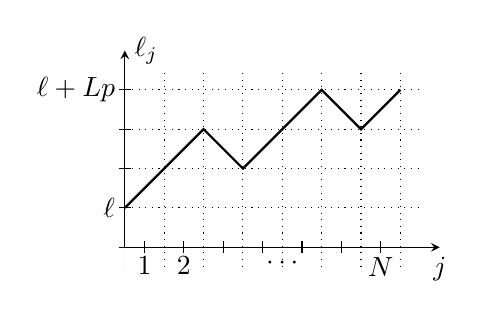
\begin{tikzpicture}[>=stealth]
     \draw[scale=0.5,thick] (0,0)--(2,2)--(3,1)--(5,3)--(6,2)--(7,3);
           
     \draw[<->] (0,2) -- (0,-0.5) -- (4,-0.5);
     \foreach \x in {0.25,0.75,...,3.25}
       \draw[xshift=\x cm,yshift=-0.5cm] (0,-0.075)--(0,0.075);
     
    \foreach \y in {-0.5,0,...,1.5}
       \draw[yshift=\y cm] (-0.075,0)--(0.075,0);
 
    \draw (0.25,-0.5) node[below] {$1$};
    \draw (0.75,-0.5) node[below] {$2$};
    \draw (2,-0.5) node[below] {$\cdots$};
    \draw (3.25,-0.5) node[below] {$N$};
    \draw (4,-0.5) node[below] {$j$};
    \draw (0,0) node [left] {$\ell$};
    \draw (0,1.5) node [left] {$\ell+Lp$};
    \draw (0,2) node [right] {$\ell_j$};
    \clip[scale=0.5] (0,-1.5) rectangle (7.5,3.5);
    \draw[scale=0.5,dotted] (-1,-2) grid (8,5);
  \end{tikzpicture}
}
  
\end{texexample}




%\begin{texexample}{Example}{}
%\newcommand{\ud}{\ensuremath \mathop{}\!\mathrm{d}}
%\(z=2\sin x\mathrm{d}x\) and \(z=2\sin x\ud x\)
%
%
%\newcommand{\ud}{\mathop{}\!\mathrm{d}}
%\bigskip
%
%It uses an empty operator and eliminates the space
%on its left with |\!|.
%
%Note the difference between
%
%\[z=2\sin x\mathrm{d}x  \]
%
%\[z=2\sin x\ud x\]
%
%where the diffrential is obtained respectively with
%|\mathrm{d}| and |\ud|.
%\end{texexample}




\subsubsection{God is in the details}

Sometimes you will be faced with small decisions for which the Journal style manual might not have an answer for you or the journal Editor might have a different opinion to yours. One such question is if one needs to insert the thousand separator in coefficients.

\[
\operatorname{erf}^{-1}(z)=\tfrac{1}{2}\sqrt{\pi}\left (z+\frac{\pi}{12}z^3+\frac{7\pi^2}{480}z^5+\frac{127\pi^3}{40320}z^7+\frac{4369\pi^4}{5806080}z^9+\frac{34807\pi^5}{182476800}z^{11}+\cdots\right )
\]


\[
\operatorname{erf}^{-1}(z)=\tfrac{1}{2}\sqrt{\pi}\left (z+\frac{\pi}{12}z^3+\frac{7\pi^2}{480}z^5+\frac{127\pi^3}{40,320}z^7+\frac{4,369\pi^4}{5,806,080}z^9+\frac{34,807\pi^5}{182{,}476,800}z^{11}+\cdots\right )
\]

\[
\operatorname{erf}^{-1}(z)=\tfrac{1}{2}\sqrt{\pi}\left (z+\frac{\pi}{12}z^3+\frac{7\pi^2}{480}z^5+\frac{127\pi^3}{40{,}320}z^7+\frac{4{,}369\pi^4}{5{,}806{,}080}z^9+\frac{34{,}807\pi^5}{182{,}476{,}800}z^{11}+\cdots\right )
\]



\[
\operatorname{erf}^{-1}(z)=\tfrac{1}{2}\sqrt{\pi}\left (z+\frac{\pi}{12}z^3+\frac{7\pi^2}{480}z^5+\frac{127\pi^3}{40\thinspace 320}z^7+\frac{4\thinspace 369\pi^4}{5\thinspace 806\thinspace 080}z^9+\frac{34\thinspace 807\pi^5}{182\thinspace 476\thinspace 800}z^{11}+\cdots\right )
\]


If you type the commas watch out to put them in |{,}| otherwise \tex's algorithm will leave a space. See the difference below:

\[182{,}476{,}800 \]
\[182,476,800\]

It is interesting to note that Knuth believes that in equations this is unnecessary.
He is quoted in Typesetting Mathematics.


\begin{quotation}
But where Don wrote 1000000 they substituted
1,000,000. Don objected that although this might be justifed in text, his use is perfectly OK in a formula. Well then, they replied, write \(10^6\).
Fine, said, Don, but what do I do 
when the number is 1234567? The IEEE standard here is to insert spaces, thus: 1 234 567.
Don doesn't like this in formulae, but agrees that it may be useful in a high precision context, such as numerical tables. 
\end{quotation}



The following are extracts from his paper \textit{Johann Faulhaber and Sums of Powers}:\footnote{\url{http://www-cs-faculty.stanford.edu/~uno/papers/jfsp.tex.gz}}

{
\[\vcenter{\halign{$#$\hfil\ &$#$\hfil\cr
\Sigma n^{11}&=39916800{n+6\choose 12}+
19958400{n+5\choose 10}+3160080{n+4\choose 8}
+168960{n+3\choose 6}\cr
\noalign{\smallskip}
&\qquad\null+2046{n+2\choose 4}+{n+1\choose 2}\,;\cr
\noalign{\smallskip}
\Sigma n^{13}&=6227020800{n+7\choose 14}+3632428800{n+6\choose 12}+
726485760{n+5\choose 10}\cr
\noalign{\smallskip}
&\qquad\null+57657600{n+4\choose 8}
+1561560{n+3\choose 6}+8190{n+2\choose 4}+\binom{n+1}{2}\,.\cr}}\]
}

Also, note in the last equation the use of a period at the end. 
This is something that evokes strong opinions and flaming wars in fora. 
I am not too sure if I agree on the last one, but the way that Knuth writes 
is very clear and his equations in a way are paragraphs. 
In this case the use of a period is recommended.


\subsection{Punctuation}
\index{maths>typography>punctuation}

There are two schools of thought when it comes to punctuation, that is punctuation in display style formulae. Some authors (Beccari, 2007) argue it is not necessary, others that it is necessary and essential \footcite{guiggiani2008}. Mermin \footcite{mermin89} strongly argued in his third rule that:  `The
Math Is Prose rule simply says: End
a displayed equation with a punctuation
mark. It is implicit in this
statement that the absence of a punctuation
mark is itself a degenerate
form of punctuation that, like periods,
commas or semicolons, can be used
provided it makes sense.''

The authors of this article believe that equations, both in display and text style, are part of the argumentation
and so punctuation should be used to help the reader. An example of good use of punctuation is:


Since
\[ a=b \]
and
\[ b=c,\]
it is proven that
\[ a =c. \]

It is extremely unusual to find an equation end with a question mark but here is one. What is 
\[ a = d^2\mathrm{?} \]

If you do put a question mark or an exclamation mark and you are using unicode fonts,
you will need to use |\mathrm{?}| not to confuse it with the relevant symbols.

Most journals require that equations be punctuated, like normal text. Even if the author of the manuscript disagrees, probably the journal editor will add the punctuation.

Read your mathematical text aloud and introduce punctuation as if it was spelled in words rather than mathematical symbols. 

\subsection{Numbering Equations}
\index{maths>typography>equation numbering}

One question that you may face is the numbering of display equations. Early books used numbering sparingly, whereas many authors go overboard and number all the equations.

According to Knuth et al:\footnote{\url{http://tex.loria.fr/typographie/mathwriting.pdf}}
Numbering all displayed formulas is usually a bad idea; number the important ones only.

Halmos\footnote{\url{http://www.math.uh.edu/~tomforde/Books/Halmos-How-To-Write.pdf}} offers pretty much the same good advice,

\begin{latexquotation}
What about ``inequality (*)", or ``equation (7)", or ``formula (iii)"; should all displays be labelled or numbered? My answer is no. Reason: just as you shouldn't mention irrelevant assumptions or name irrelevant concepts, you also shouldn't attach irrelevant labels. Some small part of the reader's attention is attracted to the label, and some small part of his mind will wonder why the label is there. If there is a reason, then the wonder serves a healthy purpose by way of preparation, with no fuss, for a future reference to the same idea; if there is no reason, then the attention and the wonder were wasted.
\end{latexquotation}

Mermin's argues in his Good samaritan Rule: that it is distressing to having to hunt for an equation back in a manuscript for Eq. (2.46) not because your subsequent progress requires
you to inspect it in detail, but merely to find out what it is about so
you may know the principles that go into the construction of Eq. (7.38).
The Good Samaritan rule says: When referring to an equation identify it by
a phrase as well as a number. No compassionate and helpful person
would herald the arrival of Eq. (7.38) by saying "inserting (2.47) and (3.51)
into (5.13)..." when it is possible to say "inserting the form (2.47) of the
electric field $E$ and the Lindhard form (3.51) of the dielectric function $e$ into
the constitutive equation (5.13). To be sure, it's longer this way but much 
clearer\ldots'

For those that want only the equations that are referenced numbered the package \pkgname{autoref} can automate this. This is not included in this package due to conflicts with \pkgname{mathtools} and \pkgname{amsmath}.
\footnote{See also discussion at \protect\url{http://tex.stackexchange.com/questions/29267/which-equations-should-be numbered/49080\#49080}}

Now if you wish to argue about this is fine.

\section{Mathmode}

\tex is in \textit{mathmode} when it is reading mathematics. The |ifmmode| can be used to find out if \tex is in math mode. It denotes the start of an if-then-else control structure that tests whether \tex is currently in either math mode or display math mode. The |\else| part is optional. <TeX code 1> is processed if TeX is in one of the math modes, otherwise it is ignored. 
If the |\else| section is included and TeX is not in one of the math modes then \meta{TeX code 2} is processed; otherwise it is ignored.


\begin{texexample}{Calligraphic fonts}{ex:cal}

\newcommand{\Acal}{\ifmmode \mathcal{Acal} \else \(\mathcal{Acal}\) \fi}
The commandd efines a macro |\Acal| that can be used both in and out of math mode to typeset a calligraphy script A. 

This is a calligraphic {\Acal} or ({\Acal}).
\end{texexample}


\section{Useful packages}

Besides the main packages that we have discussed so far and which should be in everyone's toolbox, there are a number of other packages that you may find useful. One such package is the \pkgname{multienum}, which although not really a packaged specializing in mathematical typesetting, it provides an environment to set multiple equations, as in an exercise or exam.



\subsection{the multienum package}

The \docpkg{multienum} enables  the typestting of multiple equations on one line and numbering them, either with roman, arabic or alpha letters.

\emphasis{usepackage, multienum,begin,end,multienumerate}
\begin{teXXX}
\documentclass{article}
\usepackage{multienum}
\renewcommand{\regularlisti}{\setcounter{multienumi}{0}%
  \renewcommand{\labelenumi}%
  {\addtocounter{multienumi}{1}\alph{multienumi})}}
\begin{document}
\begin{multienumerate}[oddlist]
\mitemxxx{\(x^2 + y^2 = 1\)}{\(a + b = c\)}{\(r-x = y+z\)}
\mitemxxx{\(f - y = z\)}{\(a - b = 2d\)}{\(r+x = 2y-3z\)}
\end{multienumerate}
\end{document}
\end{teXXX}


\begin{multienumerate}[oddlist]
\mitemxxx{\(x^2 + y^2 = 1\)}{\(a + b = c\)}{\(r-x = y+z\)}
\end{multienumerate}
\begin{multienumerate}[evenlist]
\mitemxxx{\(f - y = z\)}{\(a - b = 2d\)}{\(r+x = 2y-3z\)}
\end{multienumerate}


\hrule

\bigskip

We can also enumerate the items using an even-only or odd only
counter.
\subsection*{Answers to Even-Numbered Exercises}
\begin{multienumerate}[evenlist]
\mitemxxxx{Not}{Linear}{Not}{Quadratic}
\mitemxxxo{Not}{Linear}{No; if $x=3$, then $y=-2$.}
\mitemxx{$(x_1,x_2)=(2+\frac{1}{3}t,t)$ or
$(s,3s-6)$}{$(x_1,x_2,x_3)=(2+\frac{5}{2}s-3t,s,t)$}
\mitemx{$(x_1,x_2,x_3,x_4)= (\frac{1}{4}+\frac{5}{4}s+\frac{3}{4}t-u,s,t,u)$
or $(s,t,u,\frac{1}{4}-s+\frac{5}{4}t+\frac{3}{4}u)$}
\mitemxxxx{$(2,-1,3)$}{None}{$(2,1,0,1)$}{$(0,0,0,0)$}
\end{multienumerate}
\bigskip



\newcommand\thecasestudylabel{Case Study}
\newenvironment{casestudy}[2][]{%
   \clearpage\par\leavevmode
   \addcontentsline{toc}{section}{\thecasestudylabel:  #1}
    \topline\vskip1.5pt
   {\noindent\large CASE STUDY\par}\vspace{3.5pt}
   \noindent\textsc{\large#1}\par
   \bigskip
   {#2}
   \medskip
   \topline
}{%
\vfill\bottomline}

\begin{casestudy}[The Riemann hypothesis.]{%
Typeset the text and the equations, shown below. Use a standard minimal to achieve it. Note the fraktur fonts. Text must all be as one paragraph.}

It is well known that the Riemann zeta function $\zeta(s)$ of a complex variable $s=\sigma+it$ is defined by
\[
\zeta(s)=\sum_{n=1}^{\infty}\frac{1}{n^{s}}
\]
for the real part $\mathfrak{R}(s)>1$ and its analytic continuation in the half plane $\sigma>0$ is
\begin{equation}\label{func:zeta}
\zeta(s)=\sum_{n=1}^{N}\frac{1}{n^{s}}-\frac{N^{1-s}}{1-s}-\frac{1}{2}N^{-s}
+s\int_{N}^{\infty}\frac{\frac{1}{2}-\{x\}}{x^{s+1}}dx
\end{equation}
for any integer $N\geq1$ and $\mathfrak{R}(s)>0$.
It extends to an analytic function in the whole complex plane except for having a simple pole at $s=1$. Trivially, $\zeta(-2n)=0$ for all positive integers. All other zeros of the Riemann zeta functions are called its nontrivial zeros.
\bottomline

\begin{teX}
It is well known that the Riemann zeta function $\zeta(s)$ of a complex variable $s=\sigma+it$ is defined by
\[
\zeta(s)=\sum_{n=1}^{\infty}\frac{1}{n^{s}}
\]
for the real part $\mathfrak{R}(s)>1$ and its analytic continuation in the half plane $\sigma>0$ is
\begin{equation}\label{func:zeta}
\zeta(s)=\sum_{n=1}^{N}\frac{1}{n^{s}}-\frac{N^{1-s}}{1-s}-\frac{1}{2}N^{-s}
+s\int_{N}^{\infty}\frac{\frac{1}{2}-\{x\}}{x^{s+1}}dx
\end{equation}
for any integer $N\geq1$ and $\mathfrak{R}(s)>0$.
It extends to an analytic function in the whole complex plane except for having a simple pole at $s=1$. Trivially, $\zeta(-2n)=0$ for all positive integers. All other zeros of the Riemann zeta functions are called its nontrivial zeros.
\end{teX}

Please note that the maths and the text, are typed as a single block. Do not leave any spaces in between. We have used |\mathfrak| for the fraktur font. We have also used $it$ for the imaginary part. This would depend on the style used in your field. 
\end{casestudy}

\clearpage
\section{Gather}

\begin{docEnvironment}{gather}{}
This is like a multi line environment with no special horizontal alignment. All rows
are centered and can have an own equation number:
\end{docEnvironment}

\begin{texexample}{Gather}{ex:gather}
\begingroup
\def\O{\mathcal{O}}
\begin{gather}
 \O,\O(E_4),\O(E_2),\O(H-E_3-E_5),\O(H-E_3),\O(H-E_5),\\ 
\O(2H-E_1-E_3-E_5-E_6),\O(2H-E_1-E_3-E_5),\O(2H-E_3-E_5-E_6).
\end{gather}

So lautet der Beweis des Satzes $2 \times 2 = 4$:
\begin{gather}
(\Omega^{\nu})^{\mu}{}'x = \Omega^{\nu \times \mu}{}'x \text{ Def.}\\
%\begin{split}
\Omega^{2 \times 2}{}'x = (\Omega^{2})^{2}{}'x = (\Omega^{2})^{1 + 1}{}'x = \Omega^{2}{}'\Omega^{2}{}'x = \Omega^{1 + 1}{}'\Omega^{1 + 1}{}'x\nonumber \\
= (\Omega'\Omega)'(\Omega'\Omega)'x = \Omega'\Omega'\Omega'\Omega'x = \Omega^{1 + 1 + 1 + 1}{}'x = \Omega^{4}{}'x.
%\end{split}
\end{gather}


\begin{gather*}
  x = \Omega^{0}{}' x \text{ Def.\ and}\\
  \Omega'\Omega^{\nu}{}'x = \Omega^{\nu+1}{}'x \text{ Def.}
\end{gather*}
\begin{equation}
  x = \Omega^{0}{}' x \text{ Def.\ and}\\
\Omega'\Omega^{\nu}{}'x = \Omega^{\nu+1}{}'x \text{ Def.}
\end{equation}
\endgroup
\end{texexample}


\section{How to number equations either to the left or right?}
\label{eqnochange}

\latexe uses Plain TeX \docAuxCommand{eqno} and \docAuxCommand{leqno} to place the equation number either to the left or the right of the equation. The placement is done automatically and the recommended way is to set this through the documentclass declaration at the start of the document. This can also be set manually later on through the above control sequences, as shown in the Example~\ref{ex:eqno}.

\begin{texexample}{Left or right numbering}{ex:eqno}
\makeatletter
\[ a = b + x^2 \eqno \@eqnnum \]
or at left
\[ a = b + x^2 \leqno \@eqnnum \]
\makeatother
\end{texexample}


%\meaning\text

%\chapter{Unicode Math}
\tcbdocmarginnote{N 29-06-2018}
Unicode contains separate codepoints for most if not all variations of alphabet
shape one may wish to use in mathematical notation. The complete list is shown
in table 5. Some of these have been covered in the previous sections.
The math font switching commands do not nest; therefore if you want sans
serif bold, you must write |\mathbfsf{...}| rather than |\mathbf{\mathsf{...}}|.
This may change in the future.

\section{Unicode maths font setup}

The promise of Unicode is that all symbols and alphabetic variants are in one font. The \pkgname{unicode-math}
maps all the available unicode math characters of a math font to respective \latex commands. If you have patience you can actually input them directly from the keyboard rather than in commands.

The best advice that I can give you is to read the \pkgname{unicode-math} carefully. 

\begin{docCommand} {setmathfont} { \oarg{range=\meta{unicode range}, \meta{font features } } \marg{font name} }
In many cases using one font might not be adequate. Specific Unicode ranges can be assigned to separate fonts.
\end{docCommand}

\subsection{Control over maths alphabets}

\subsection{Math `versions'}

\subsection{Maths input}

\subsection{Math `style'}

\subsubsection{Bold style}

Similar as in the previous section, ISO standards differ somewhat to \tex’s conventions
(and classical typesetting) for ‘boldness’ in mathematics. In the past, it has
been customary to use bold upright letters to denote things like vectors and matrices.


$$\boldsymbol{\omega} \times \mathbf{T} = \mathbf{T'}$$

$$\mathbf{\omega} = {1\over 2}\kappa \mathbf{B} + {1\over 2}(\kappa \mathbf{B} + \tau \mathbf{T}) + {1\over 2}\tau \mathbf{T} = \kappa \mathbf{B} + \tau \mathbf{T}
$$

\[
\mathbf{e} = \frac{\mathbf{A}}{m k} = \frac{1}{m k}(\mathbf{p} \times \mathbf{L})
\]

\subsubsection{Sans serif style}

\subsubsection{Blackboard or double-struck}



\subsubsection{Caligraphic and Script variants}



\section{Growing and non-growing accents}

This are the most problematic with Unicode fonts.

%%%%%%%% INPUT INTEGRAL FILES %%%%%%%%%%
%%%%%%%%%%%%%%%%%%%%%%%%%%%%%%%
 %% Too many errors here need to revisit.
 \subsection{Delimiters}
 \begin{multicols}{2}
% \showmbrace/{002F}{}
% \showlbrace({0028}{}
% \showlbrace[{005B}{}
% \showlbrace\lbrace{007B}{}
% \showmbrace\backslash{005C}{}
% \showrbrace){0029}{}
% \showrbrace]{005D}{}
% \showrbrace\rbrace{007D}{}
% \showlbrace\lceil{2308}{}
% \showlbrace\lfloor{230A}{}
% \showlbrace\lmoustache{23B0}{*}
% \showlbrace\lbrbrak{2772}{*}
% \showlbrace\lBrack{27E6}{*}
% \showlbrace\langle{27E8}{}, \cmd<
% \showlbrace\lAngle{27EA}{*}
% \showlbrace\lgroup{27EE}{*}
% \showlbrace\lBrace{2983}{*}
% \showlbrace\lParen{2985}{*}
% \showrbrace\rceil{2309}{}
 %\showrbrace\rfloor{230B}{}
% \showrbrace\rmoustache{23B1}{*}
% \showrbrace\rbrbrak{2773}{*}
% \showrbrace\rBrack{27E7}{*}
% \showrbrace\rangle{27E9}{}, \cmd>
% \showrbrace\rAngle{27EB}{*}
% \showrbrace\rgroup{27EF}{*}
 %\showrbrace\rBrace{2984}{*}
% \showrbrace\rParen{2986}{*}
 \end{multicols}

 \begin{multicols}{2}
% \showmbrace\vert{007C}{}, \cmd|
 \showmbrace\Vert{2016}{*}, \cmd\|
 \showmbrace\Vvert{2980}{}
 \showmbrace\uparrow{2191}{}
 \showmbrace\downarrow{2193}{}
 \showmbrace\updownarrow{2195}{}
 \showmbrace\Uparrow{21D1}{}
 \showmbrace\Downarrow{21D3}{}
 \showmbrace\Updownarrow{21D5}{}
% \showmbrace\Uuparrow{290A}{*}
% \showmbrace\Ddownarrow{290B}{*}
% \showmbrace\UUparrow{27F0}{*}
% \showmbrace\DDownarrow{27F1}{*}
% \showmbrace\arrowvert{XXXX}{}
% \showmbrace\Arrowvert{XXXX}{}
% \showmbrace\bracevert{XXXX}{*}
 \end{multicols}

 \subsection{Other bracess}
 \begin{multicols}{2}
 \showsymbol\ulcorner{231C}{*}
 \showsymbol\urcorner{231D}{*}
 \showsymbol\llcorner{231E}{*}
 \showsymbol\lrcorner{231F}{*}
 \showsymbol\Lbrbrak{27EC}{*}
 \showsymbol\Rbrbrak{27ED}{*}
 \showsymbol\llparenthesis{2987}{*}
 \showsymbol\rrparenthesis{2988}{*}
 \showsymbol\llangle{2989}{*}
 \showsymbol\rrangle{298A}{*}
 \showsymbol\lbrackubar{298B}{*}
 \showsymbol\rbrackubar{298C}{*}
 \showsymbol\lbrackultick{298D}{*}
 \showsymbol\rbracklrtick{298E}{*}
 \showsymbol\lbracklltick{298F}{*}
 \showsymbol\rbrackurtick{2990}{*}
 \showsymbol\langledot{2991}{*}
 \showsymbol\rangledot{2992}{*}
 \showsymbol\lparenless{2993}{*}
 \showsymbol\rparengtr{2994}{*}
 \showsymbol\Lparengtr{2995}{*}
 \showsymbol\Rparenless{2996}{*}
 \showsymbol\lblkbrbrak{2997}{*}
 \showsymbol\rblkbrbrak{2998}{*}
 \showsymbol\lvzigzag{29D8}{*}
 \showsymbol\rvzigzag{29D9}{*}
 \showsymbol\Lvzigzag{29DA}{*}
 \showsymbol\Rvzigzag{29DB}{*}
 \showsymbol\lcurvyangle{29FC}{*}
 \showsymbol\rcurvyangle{29FD}{*}
 \showsymbol\lbrbrak{2772}{*}
 \showsymbol\rbrbrak{2773}{*}
 \showsymbol\lbag{27C5}{*}
 \showsymbol\rbag{27C6}{*}
 \showsymbol\Lbrbrak{27EC}{*}
 \showsymbol\Rbrbrak{27ED}{*}
 \end{multicols}

 \section{Alphabetics}
 \begin{multicols}{2}
\showsymbolalpha\Gamma{0393}{}
\showsymbolalpha\Delta{0394}{}
\showsymbolalpha\Theta{0398}{}
\showsymbolalpha\Lambda{039B}{}
\showsymbolalpha\Xi{039E}{}
\showsymbolalpha\Pi{03A0}{}
\showsymbolalpha\Sigma{03A3}{}
\showsymbolalpha\Upsilon{03A5}{}
\showsymbolalpha\Phi{03A6}{}
\showsymbolalpha\Psi{03A8}{}
\showsymbolalpha\Omega{03A9}{}
\showsymbolalpha\alpha{03B1}{}
\showsymbolalpha\beta{03B2}{}
\showsymbolalpha\gamma{03B3}{}
\showsymbolalpha\delta{03B4}{}
\showsymbolalpha\epsilon{03B5}{}
\showsymbolalpha\zeta{03B6}{}
\showsymbolalpha\eta{03B7}{}
\showsymbolalpha\theta{03B8}{}
\showsymbolalpha\iota{03B9}{}
\showsymbolalpha\kappa{03BA}{}
\showsymbolalpha\lambda{03BB}{}
\showsymbolalpha\mu{03BC}{}
\showsymbolalpha\nu{03BD}{}
\showsymbolalpha\xi{03BE}{}
\showsymbolalpha\pi{03C0}{}
\showsymbolalpha\rho{03C1}{}
\showsymbolalpha\sigma{03C3}{}
\showsymbolalpha\tau{03C4}{}
\showsymbolalpha\upsilon{03C5}{}
\showsymbolalpha\phi{03D5}{}
\showsymbolalpha\chi{03C7}{}
\showsymbolalpha\psi{03C8}{}
\showsymbolalpha\omega{03C9}{}
\showsymbolalpha\varepsilon{03F5}{}
\showsymbolalpha\vartheta{03D1}{}
\showsymbolalpha\varpi{03D6}{}
\showsymbolalpha\varrho{03F1}{}
\showsymbolalpha\varsigma{03C2}{}
\showsymbolalpha\varphi{03C6}{}
\showsymbolalpha\nabla{2207}{}
\showsymbolalpha\partial{2202}{}
\showsymbolalpha\imath{1D6A4}{}
\showsymbolalpha\jmath{1D6A5}{}
 \end{multicols}
% \subsection{Accents}
 \begin{multicols}{2}
 \showaccent\grave{0300}{}
 \showaccent\acute{0301}{}
 \showaccent\hat{0302}{}
 \showaccent\tilde{0303}{}
 \showaccent\bar{0304}{}
 \showaccent\breve{0306}{}
 \showaccent\dot{0307}{}
 \showaccent\ddot{0308}{}
 \showaccent\ovhook{0309}{}
 \showaccent\mathring{030A}{}
 \showaccent\check{030C}{}
 \showaccent\candra{0310}{}
 \showaccent\oturnedcomma{0312}{}
 \showaccent\ocommatopright{0315}{}
 \showaccent\droang{031A}{}
 \showaccent\leftharpoonaccent{20D0}{}
 \showaccent\rightharpoonaccent{20D1}{}
 %\showaccent\leftarrowaccent{20D6}{}
 \showaccent\vec{20D7}{}, \cmd\rightarrowaccent
 %\showaccent\leftrightarrowaccent{20E1}{}
 \showaccent\dddot{20DB}{}
 \showaccent\ddddot{20DC}{}
 \showaccent\annuity{20E7}{}
 \showaccent\widebridgeabove{20E9}{}
 \showaccent\asteraccent{20F0}{}
 \end{multicols}

 \begin{multicols}{2}
 \showwideaccent\widehat{0302}{*}
 \showwideaccent\widetilde{0303}{*}
% \showwideaccent\widecheck{030C}{*}
 \showwideaccent\overleftarrow{20D6}{}
 \showwideaccent\overrightarrow{20D7}{}
 \showwideaccent\underrightarrow{20EF}{}
 \showwideaccent\underleftarrow{20EE}{}
 \showwideaccent\overleftrightarrow{20E1}{}
 \showwideaccent\underleftrightarrow{034D}{}
% \showwideaccent\overleftharpoon{20D0}{}
% \showwideaccent\overrightharpoon{20D1}{}
% \showwideaccent\underleftharpoon{20EC}{}
% \showwideaccent\underrightharpoon{20ED}{}
 \end{multicols}

 OpenType STIX fonts include a number of under accents that can be used in
 math mode, but \TeX\ does not support under accents natively so such glyphs
 can not be used directly. Under accents can be set using regular accents and
 commands like |\underaccent| from the \pkgname{accents} package, for example
 gives |\(\underaccent{\hat}{X}\)|. The
 \pkgname{undertilde} package provides |\utilde| for extensible under tilde
 accent \citep{undertilde}.
 
 
 % \subsection{Over and under brackets}
 \begin{multicols}{2}
 %\showover\overbracket{23B4}{} conflict mathtools consider remove mathtools for UNICODE
 \showover\overparen{23DC}{}
 \showover\overbrace{23DE}{}
 \showover\underbracket{23B5}{} %conflict mathtools?
 \showover\underparen{23DD}{}
 \showover\underbrace{23DF}{}
 \end{multicols}

 \subsection{Radicals}
 \begin{multicols}{2}
 \showaccent\sqrt{221A}{}
 \showaccent\longdivision{27CC}{*}
 \end{multicols}
 
 
 
 
 
 
 \subsection{Big operators}
 \begin{multicols}{2}
 \showop\Bbbsum{2140}{}
 \showop\prod{220F}{}
 \showop\coprod{2210}{}
 \showop\sum{2211}{}
 \showop\bigwedge{22C0}{}
 \showop\bigvee{22C1}{}
 \showop\bigcap{22C2}{}
 \showop\bigcup{22C3}{}
 \showop\leftouterjoin{27D5}{*}
 \showop\rightouterjoin{27D6}{*}
 \showop\fullouterjoin{27D7}{*}
 \showop\bigbot{27D8}{*}
 \showop\bigtop{27D9}{*}
 \showop\xsol{29F8}{*}
 \showop\xbsol{29F9}{*}
 \showop\bigodot{2A00}{*}
 \showop\bigoplus{2A01}{*}
 \showop\bigotimes{2A02}{*}
 \showop\bigcupdot{2A03}{*}
 \showop\biguplus{2A04}{*}
 \showop\bigsqcap{2A05}{*}
 \showop\bigsqcup{2A06}{*}
 \showop\conjquant{2A07}{*}
 \showop\disjquant{2A08}{*}
 \showop\bigtimes{2A09}{*}
 \showop\modtwosum{2A0A}{*}
 \showop\Join{2A1D}{*}
 \showop\bigtriangleleft{2A1E}{*}
 \showop\zcmp{2A1F}{*}
 \showop\zpipe{2A20}{*}
 \showop\zproject{2A21}{*}
 \showop\biginterleave{2AFC}{}
 \showop\bigtalloblong{2AFF}{*}
 \end{multicols}
 
 \section{General manipulations test.}
 
 Here are some examples using big operators

$$\sum_{n=s}^t C\cdot f(n) = C\cdot \sum_{n=s}^t f(n),$$ where ``'C'' is a constant

\[\sum_{n=s}^t f(n) + \sum_{n=s}^{t} g(n) = \sum_{n=s}^t \left[f(n) + g(n)\right]\] 

\[\sum_{n=s}^t f(n) - \sum_{n=s}^{t} g(n) = \sum_{n=s}^t \left[f(n) - g(n)\right]\] 

\[\sum_{n=s}^t f(n) = \sum_{n=s+p}^{t+p} f(n-p) \] 

\[\sum_{n\in B} f(n) = \sum_{m\in A} f(\sigma(m)),\] for a bijection σ from a finite set ``$A$'' onto a finite set ``$B$''; this generalizes the preceding formula.

\[\sum_{n=s}^j f(n) + \sum_{n=j+1}^t f(n) = \sum_{n=s}^t f(n)\] 

\[\sum_{i=k_0}^{k_1}\sum_{j=l_0}^{l_1} a_{i,j} = \sum_{j=l_0}^{l_1}\sum_{i=k_0}^{k_1} a_{i,j}\] 

\[\sum_{k\le j \le i\le n} a_{i,j} = \sum_{i=k}^n\sum_{j=k}^i a_{i,j} = \sum_{j=k}^n\sum_{i=j}^n a_{i,j}\] 


\[\sum_{n=0}^t f(2n) + \sum_{n=0}^t f(2n+1) = \sum_{n=0}^{2t+1} f(n)\] 

\[\sum_{n=0}^t \sum_{i=0}^{z-1} f(z\cdot n+i) = \sum_{n=0}^{z\cdot t+z-1} f(n)\] 

\[\sum_{i=s}^m\sum_{j=t}^n {a_i}{c_j} = \sum_{i=s}^m a_i \cdot \sum_{j=t}^n c_j\] 

\[\sum_{n=s}^t \ln f(n) = \ln \prod_{n=s}^t f(n)\] 

\[c^{\left[\sum_{n=s}^t f(n) \right]} = \prod_{n=s}^t c^{f(n)}\] 
 
 
 \section{Convergence criteria}
 
The product of positive real numbers

\[\prod_{n=1}^{\infty} a_n\]
converges to a nonzero real number if and only if the sum
\[\sum_{n=1}^{\infty} \log(a_n)\]
converges. This allows the translation of convergence criteria for infinite sums into convergence criteria for infinite products. The same criterion applies to products of arbitrary complex numbers (including negative reals) if log is understood as a fixed Complex logarithm which satisfies $\log(1) = 0$, with the proviso that the infinite product diverges when infinitely many ''$a_n$'' fall outside 
the domain of log, whereas finitely many such ''$a_n$'' can be ignored in the sum.

For products of reals in which each $a_n\ge1$, written as, for instance, $a_n=1+p_n$,
where $p_n\ge 0$, the bounds

\[1+\sum_{n=1}^{N} p_n \le \prod_{n=1}^{N} \left( 1 + p_n \right) \le \exp \left( \sum_{n=1}^{N}p_n \right)\]

show that the infinite product converges precisely if the infinite sum of the $p_n$ converges. This relies on the Monotone convergence theorem. More generally, the convergence of $\prod_{n=1}^\infty(1+p_n)$ is equivalent to the convergence of $\sum_{n=1}^\infty p_n$ 
%if ''p<sub>n</sub>'' are real or complex numbers such that <math>\sum_{n=1}^\infty|p_n|^2<+\infty\], since <math>\log(1+x)=x+O(x^2)\] in a neighbourhood of 0.
%
%If the series ''p''<sub>''n''</sub> diverges, then the sequence of partial products converges to zero as a sequence.  The infinite product is said to '''diverge to zero'''.
% 
 
 
 
 
 
 
 
 
%% Relations symbols from STIX font
%% 
  \subsection{Relations}
 \begin{multicols}{2}
% \showrelsymbol*{002A}{}, \cmd\ast
% \showrelsymbol:{003A}{}
 \showrelsymbol{\less}{003C}{}, \cmd\less
 \showrelsymbol{\equal}{003D}{}, \cmd\equal
 \showrelsymbol{\greater}{003E}{}, \cmd\greater
 \showrelsymbol\closure{2050}{*}
 %\showrelsymbol\vertoverlay{20D2}{}
 \showrelsymbol\leftarrow{2190}{}, \cmd\gets
 \showrelsymbol\uparrow{2191}{}
 \showrelsymbol\rightarrow{2192}{}, \cmd\to
 \showrelsymbol\downarrow{2193}{}
 \showrelsymbol\leftrightarrow{2194}{}
 \showrelsymbol\updownarrow{2195}{}
 \showrelsymbol\nwarrow{2196}{}
 \showrelsymbol\nearrow{2197}{}
 \showrelsymbol\searrow{2198}{}
 \showrelsymbol\swarrow{2199}{}
 \showrelsymbol\nleftarrow{219A}{}
 \showrelsymbol\nrightarrow{219B}{}
 \showrelsymbol\leftwavearrow{219C}{}
 \showrelsymbol\rightwavearrow{219D}{}
 \showrelsymbol\twoheadleftarrow{219E}{}
 \showrelsymbol\twoheaduparrow{219F}{}
 \showrelsymbol\twoheadrightarrow{21A0}{}
 \showrelsymbol\twoheaddownarrow{21A1}{}
 \showrelsymbol\leftarrowtail{21A2}{}
 \showrelsymbol\rightarrowtail{21A3}{}
 \showrelsymbol\mapsfrom{21A4}{}
 \showrelsymbol\mapsup{21A5}{}
 \showrelsymbol\mapsto{21A6}{}
 \showrelsymbol\mapsdown{21A7}{}
 \showrelsymbol\hookleftarrow{21A9}{}
 \showrelsymbol\hookrightarrow{21AA}{}
 \showrelsymbol\looparrowleft{21AB}{}
 \showrelsymbol\looparrowright{21AC}{}
 \showrelsymbol\leftrightsquigarrow{21AD}{}
 \showrelsymbol\nleftrightarrow{21AE}{}
 \showrelsymbol\downzigzagarrow{21AF}{}
 \showrelsymbol\Lsh{21B0}{}
 \showrelsymbol\Rsh{21B1}{}
 \showrelsymbol\Ldsh{21B2}{}
 \showrelsymbol\Rdsh{21B3}{}
 \showrelsymbol\curvearrowleft{21B6}{}
 \showrelsymbol\curvearrowright{21B7}{}
 \showrelsymbol\circlearrowleft{21BA}{}
 \showrelsymbol\circlearrowright{21BB}{}
 \showrelsymbol\leftharpoonup{21BC}{}
 \showrelsymbol\leftharpoondown{21BD}{}
 \showrelsymbol\upharpoonright{21BE}{}, \cmd\restriction
 \showrelsymbol\upharpoonleft{21BF}{}
 \showrelsymbol\rightharpoonup{21C0}{}
 \showrelsymbol\rightharpoondown{21C1}{}
 \showrelsymbol\downharpoonright{21C2}{}
 \showrelsymbol\downharpoonleft{21C3}{}
 \showrelsymbol\rightleftarrows{21C4}{}
 \showrelsymbol\updownarrows{21C5}{}
 \showrelsymbol\leftrightarrows{21C6}{}
 \showrelsymbol\leftleftarrows{21C7}{}
 \showrelsymbol\upuparrows{21C8}{}
 \showrelsymbol\rightrightarrows{21C9}{}
 \showrelsymbol\downdownarrows{21CA}{}
 \showrelsymbol\leftrightharpoons{21CB}{}
 \showrelsymbol\rightleftharpoons{21CC}{}
 \showrelsymbol\nLeftarrow{21CD}{}
 \showrelsymbol\nLeftrightarrow{21CE}{}
 \showrelsymbol\nRightarrow{21CF}{}
 \showrelsymbol\Leftarrow{21D0}{}
 \showrelsymbol\Uparrow{21D1}{}
 \showrelsymbol\Rightarrow{21D2}{}
 \showrelsymbol\Downarrow{21D3}{}
 \showrelsymbol\Leftrightarrow{21D4}{}
 \showrelsymbol\Updownarrow{21D5}{}
 \showrelsymbol\Nwarrow{21D6}{}
 \showrelsymbol\Nearrow{21D7}{}
 \showrelsymbol\Searrow{21D8}{}
 \showrelsymbol\Swarrow{21D9}{}
 \showrelsymbol\Lleftarrow{21DA}{*}
 \showrelsymbol\Rrightarrow{21DB}{*}
 \showrelsymbol\leftsquigarrow{21DC}{}
 \showrelsymbol\rightsquigarrow{21DD}{}, \cmd\leadsto
 \showrelsymbol\barleftarrow{21E4}{*}
 \showrelsymbol\rightarrowbar{21E5}{*}
 \showrelsymbol\circleonrightarrow{21F4}{*}
 \showrelsymbol\downuparrows{21F5}{}
 \showrelsymbol\rightthreearrows{21F6}{*}
 \showrelsymbol\nvleftarrow{21F7}{*}
 \showrelsymbol\nvrightarrow{21F8}{*}
 \showrelsymbol\nvleftrightarrow{21F9}{*}
 \showrelsymbol\nVleftarrow{21FA}{*}
 \showrelsymbol\nVrightarrow{21FB}{*}
 \showrelsymbol\nVleftrightarrow{21FC}{*}
 \showrelsymbol\leftarrowtriangle{21FD}{*}
 \showrelsymbol\rightarrowtriangle{21FE}{*}
 \showrelsymbol\leftrightarrowtriangle{21FF}{*}
 \showrelsymbol\in{2208}{}
 \showrelsymbol\notin{2209}{}
 \showrelsymbol\smallin{220A}{}
 \showrelsymbol\ni{220B}{}, \cmd\owns
 \showrelsymbol\nni{220C}{}
 \showrelsymbol\smallni{220D}{}
 \showrelsymbol\propto{221D}{}
 \showrelsymbol\varpropto{221D}{}
 \showrelsymbol\mid{2223}{}
 \showrelsymbol\shortmid{2223}{}
 \showrelsymbol\nmid{2224}{}
 \showrelsymbol\nshortmid{2224}{*}
 \showrelsymbol\parallel{2225}{}
 \showrelsymbol\shortparallel{2225}{*}
 \showrelsymbol\nparallel{2226}{}
 \showrelsymbol\nshortparallel{2226}{*}
 \showrelsymbol\Colon{2237}{}
 \showrelsymbol\dashcolon{2239}{}
 \showrelsymbol\dotsminusdots{223A}{}
 \showrelsymbol\kernelcontraction{223B}{}
 \showrelsymbol\sim{223C}{}
 \showrelsymbol\thicksim{223C}{}
 \showrelsymbol\backsim{223D}{}
 \showrelsymbol\nsim{2241}{}
 \showrelsymbol\eqsim{2242}{}
 \showrelsymbol\simeq{2243}{}
 \showrelsymbol\nsime{2244}{}
 \showrelsymbol\cong{2245}{}
 \showrelsymbol\simneqq{2246}{}
 \showrelsymbol\ncong{2247}{}
 \showrelsymbol\approx{2248}{}
 \showrelsymbol\thickapprox{2248}{}
 \showrelsymbol\napprox{2249}{}
 \showrelsymbol\approxeq{224A}{}
 \showrelsymbol\approxident{224B}{}
 \showrelsymbol\backcong{224C}{}
 \showrelsymbol\asymp{224D}{}
 \showrelsymbol\Bumpeq{224E}{}
 \showrelsymbol\bumpeq{224F}{}
 \showrelsymbol\doteq{2250}{}
 \showrelsymbol\Doteq{2251}{}, \cmd\doteqdot
 \showrelsymbol\fallingdotseq{2252}{}
 \showrelsymbol\risingdotseq{2253}{}
 \showrelsymbol\coloneq{2254}{}
 \showrelsymbol\eqcolon{2255}{}
 \showrelsymbol\eqcirc{2256}{}
 \showrelsymbol\circeq{2257}{}
 \showrelsymbol\arceq{2258}{}
 \showrelsymbol\wedgeq{2259}{}
 \showrelsymbol\veeeq{225A}{}
 \showrelsymbol\stareq{225B}{}
 \showrelsymbol\triangleq{225C}{}
 \showrelsymbol\eqdef{225D}{}
 \showrelsymbol\measeq{225E}{}
 \showrelsymbol\questeq{225F}{}
 \showrelsymbol\ne{2260}{}, \cmd\neq
 \showrelsymbol\equiv{2261}{}
 \showrelsymbol\nequiv{2262}{}
 \showrelsymbol\Equiv{2263}{}
 \showrelsymbol\leq{2264}{}, \cmd\le
 \showrelsymbol\geq{2265}{}, \cmd\ge
 \showrelsymbol\leqq{2266}{}
 \showrelsymbol\geqq{2267}{}
 \showrelsymbol\lneqq{2268}{}
 \showrelsymbol\lvertneqq{2268}{}
 \showrelsymbol\gneqq{2269}{}
 \showrelsymbol\gvertneqq{2269}{}
 \showrelsymbol\ll{226A}{}
 \showrelsymbol\gg{226B}{}
 \showrelsymbol\between{226C}{}
 \showrelsymbol\nasymp{226D}{}
 \showrelsymbol\nless{226E}{}
 \showrelsymbol\ngtr{226F}{}
 \showrelsymbol\nleq{2270}{}
 \showrelsymbol\ngeq{2271}{}
 \showrelsymbol\lesssim{2272}{}
 \showrelsymbol\gtrsim{2273}{}
 \showrelsymbol\nlesssim{2274}{}
 \showrelsymbol\ngtrsim{2275}{}
 \showrelsymbol\lessgtr{2276}{}
 \showrelsymbol\gtrless{2277}{}
 \showrelsymbol\nlessgtr{2278}{}
 \showrelsymbol\ngtrless{2279}{}
 \showrelsymbol\prec{227A}{}
 \showrelsymbol\succ{227B}{}
 \showrelsymbol\preccurlyeq{227C}{}
 \showrelsymbol\succcurlyeq{227D}{}
 \showrelsymbol\precsim{227E}{}
 \showrelsymbol\succsim{227F}{}
 \showrelsymbol\nprec{2280}{}
 \showrelsymbol\nsucc{2281}{}
 \showrelsymbol\subset{2282}{}
 \showrelsymbol\supset{2283}{}
 \showrelsymbol\nsubset{2284}{}
 \showrelsymbol\nsupset{2285}{}
 \showrelsymbol\subseteq{2286}{}
 \showrelsymbol\supseteq{2287}{}
 \showrelsymbol\nsubseteq{2288}{}
 \showrelsymbol\nsupseteq{2289}{}
 \showrelsymbol\subsetneq{228A}{}
 \showrelsymbol\varsubsetneq{228A}{*}
 \showrelsymbol\supsetneq{228B}{}
 \showrelsymbol\varsupsetneq{228B}{*}
 \showrelsymbol\sqsubset{228F}{}
 \showrelsymbol\sqsupset{2290}{}
 \showrelsymbol\sqsubseteq{2291}{}
 \showrelsymbol\sqsupseteq{2292}{}
 \showrelsymbol\vdash{22A2}{}
 \showrelsymbol\dashv{22A3}{}
 \showrelsymbol\assert{22A6}{}
 \showrelsymbol\models{22A7}{}
 \showrelsymbol\vDash{22A8}{}
 \showrelsymbol\Vdash{22A9}{}
 \showrelsymbol\Vvdash{22AA}{}
 \showrelsymbol\VDash{22AB}{}
 \showrelsymbol\nvdash{22AC}{}
 \showrelsymbol\nvDash{22AD}{}
 \showrelsymbol\nVdash{22AE}{}
 \showrelsymbol\nVDash{22AF}{}
 \showrelsymbol\prurel{22B0}{}
 \showrelsymbol\scurel{22B1}{}
 \showrelsymbol\vartriangleleft{22B2}{}
 \showrelsymbol\vartriangleright{22B3}{}
 \showrelsymbol\trianglelefteq{22B4}{}
 \showrelsymbol\trianglerighteq{22B5}{}
 \showrelsymbol\origof{22B6}{}
 \showrelsymbol\imageof{22B7}{}
 \showrelsymbol\multimap{22B8}{}
 \showrelsymbol\bowtie{22C8}{}
 \showrelsymbol\backsimeq{22CD}{}
 \showrelsymbol\Subset{22D0}{}
 \showrelsymbol\Supset{22D1}{}
 \showrelsymbol\pitchfork{22D4}{}
 \showrelsymbol\equalparallel{22D5}{}
 \showrelsymbol\lessdot{22D6}{}
 \showrelsymbol\gtrdot{22D7}{}
 \showrelsymbol\lll{22D8}{}, \cmd\llless
 \showrelsymbol\ggg{22D9}{}, \cmd\gggtr
 \showrelsymbol\lesseqgtr{22DA}{}
 \showrelsymbol\gtreqless{22DB}{}
 \showrelsymbol\eqless{22DC}{}
 \showrelsymbol\eqgtr{22DD}{}
 \showrelsymbol\curlyeqprec{22DE}{}
 \showrelsymbol\curlyeqsucc{22DF}{}
 \showrelsymbol\npreccurlyeq{22E0}{}
 \showrelsymbol\nsucccurlyeq{22E1}{}
 \showrelsymbol\nsqsubseteq{22E2}{}
 \showrelsymbol\nsqsupseteq{22E3}{}
 \showrelsymbol\sqsubsetneq{22E4}{*}
 \showrelsymbol\sqsupsetneq{22E5}{*}
 \showrelsymbol\lnsim{22E6}{}
 \showrelsymbol\gnsim{22E7}{}
 \showrelsymbol\precnsim{22E8}{}
 \showrelsymbol\succnsim{22E9}{}
 \showrelsymbol\nvartriangleleft{22EA}{}
 \showrelsymbol\nvartriangleright{22EB}{}
 \showrelsymbol\ntrianglelefteq{22EC}{}
 \showrelsymbol\ntrianglerighteq{22ED}{}
 \showrelsymbol\vdots{22EE}{}
 \showrelsymbol\adots{22F0}{}
 \showrelsymbol\ddots{22F1}{}
 \showrelsymbol\disin{22F2}{*}
 \showrelsymbol\varisins{22F3}{*}
 \showrelsymbol\isins{22F4}{*}
 \showrelsymbol\isindot{22F5}{*}
 \showrelsymbol\varisinobar{22F6}{}
 \showrelsymbol\isinobar{22F7}{*}
 \showrelsymbol\isinvb{22F8}{*}
 \showrelsymbol\isinE{22F9}{*}
 \showrelsymbol\nisd{22FA}{*}
 \showrelsymbol\varnis{22FB}{*}
 \showrelsymbol\nis{22FC}{*}
 \showrelsymbol\varniobar{22FD}{}
 \showrelsymbol\niobar{22FE}{*}
 \showrelsymbol\bagmember{22FF}{*}
 \showrelsymbol\frown{2322}{}
 \showrelsymbol\smallfrown{2322}{*}
 \showrelsymbol\smile{2323}{}
 \showrelsymbol\smallsmile{2323}{*}
 \showrelsymbol\APLnotslash{233F}{}
 \showrelsymbol\vartriangle{25B5}{*}
 \showrelsymbol\perp{27C2}{*}
 \showrelsymbol\bsolhsub{27C8}{}
 \showrelsymbol\suphsol{27C9}{}
 \showrelsymbol\upin{27D2}{*}
 \showrelsymbol\pullback{27D3}{*}
 \showrelsymbol\pushout{27D4}{*}
 \showrelsymbol\DashVDash{27DA}{*}
 \showrelsymbol\dashVdash{27DB}{*}
 \showrelsymbol\multimapinv{27DC}{*}
 \showrelsymbol\vlongdash{27DD}{*}
 \showrelsymbol\longdashv{27DE}{*}
 \showrelsymbol\cirbot{27DF}{*}
 \showrelsymbol\UUparrow{27F0}{*}
 \showrelsymbol\DDownarrow{27F1}{*}
 \showrelsymbol\acwgapcirclearrow{27F2}{*}
 \showrelsymbol\cwgapcirclearrow{27F3}{*}
 \showrelsymbol\rightarrowonoplus{27F4}{*}
 \showrelsymbol\longleftarrow{27F5}{*}
 \showrelsymbol\longrightarrow{27F6}{*}
 \showrelsymbol\longleftrightarrow{27F7}{*}
 \showrelsymbol\Longleftarrow{27F8}{*}
 \showrelsymbol\Longrightarrow{27F9}{*}
 \showrelsymbol\Longleftrightarrow{27FA}{*}
 \showrelsymbol\longmapsfrom{27FB}{*}
 \showrelsymbol\longmapsto{27FC}{*}
 \showrelsymbol\Longmapsfrom{27FD}{*}
 \showrelsymbol\Longmapsto{27FE}{*}
 \showrelsymbol\longrightsquigarrow{27FF}{*}
 \showrelsymbol\nvtwoheadrightarrow{2900}{*}
 \showrelsymbol\nVtwoheadrightarrow{2901}{*}
 \showrelsymbol\nvLeftarrow{2902}{*}
 \showrelsymbol\nvRightarrow{2903}{*}
 \showrelsymbol\nvLeftrightarrow{2904}{*}
 \showrelsymbol\twoheadmapsto{2905}{*}
 \showrelsymbol\Mapsfrom{2906}{*}
 \showrelsymbol\Mapsto{2907}{*}
 \showrelsymbol\downarrowbarred{2908}{*}
 \showrelsymbol\uparrowbarred{2909}{*}
 \showrelsymbol\Uuparrow{290A}{*}
 \showrelsymbol\Ddownarrow{290B}{*}
 \showrelsymbol\leftbkarrow{290C}{*}
 \showrelsymbol\rightbkarrow{290D}{*}
 \showrelsymbol\leftdbkarrow{290E}{*}, \cmd\dashleftarrow
 \showrelsymbol\dbkarow{290F}{*}, \cmd\dashrightarrow
 \showrelsymbol\drbkarow{2910}{*}
 \showrelsymbol\rightdotarrow{2911}{*}
 \showrelsymbol\baruparrow{2912}{*}
 \showrelsymbol\downarrowbar{2913}{*}
 \showrelsymbol\nvrightarrowtail{2914}{*}
 \showrelsymbol\nVrightarrowtail{2915}{*}
 \showrelsymbol\twoheadrightarrowtail{2916}{*}
 \showrelsymbol\nvtwoheadrightarrowtail{2917}{*}
 \showrelsymbol\nVtwoheadrightarrowtail{2918}{*}
 \showrelsymbol\lefttail{2919}{*}
 \showrelsymbol\righttail{291A}{*}
 \showrelsymbol\leftdbltail{291B}{*}
 \showrelsymbol\rightdbltail{291C}{*}
 \showrelsymbol\diamondleftarrow{291D}{*}
 \showrelsymbol\rightarrowdiamond{291E}{*}
 \showrelsymbol\diamondleftarrowbar{291F}{*}
 \showrelsymbol\barrightarrowdiamond{2920}{*}
 \showrelsymbol\nwsearrow{2921}{*}
 \showrelsymbol\neswarrow{2922}{*}
 \showrelsymbol\hknwarrow{2923}{*}
 \showrelsymbol\hknearrow{2924}{*}
 \showrelsymbol\hksearow{2925}{*}
 \showrelsymbol\hkswarow{2926}{*}
 \showrelsymbol\tona{2927}{*}
 \showrelsymbol\toea{2928}{*}
 \showrelsymbol\tosa{2929}{*}
 \showrelsymbol\towa{292A}{*}
 \showrelsymbol\rightcurvedarrow{2933}{*}
 \showrelsymbol\leftdowncurvedarrow{2936}{*}
 \showrelsymbol\rightdowncurvedarrow{2937}{*}
 \showrelsymbol\cwrightarcarrow{2938}{*}
 \showrelsymbol\acwleftarcarrow{2939}{*}
 \showrelsymbol\acwoverarcarrow{293A}{*}
 \showrelsymbol\acwunderarcarrow{293B}{*}
 \showrelsymbol\curvearrowrightminus{293C}{*}
 \showrelsymbol\curvearrowleftplus{293D}{*}
 \showrelsymbol\cwundercurvearrow{293E}{*}
 \showrelsymbol\ccwundercurvearrow{293F}{*}
 \showrelsymbol\acwcirclearrow{2940}{*}
 \showrelsymbol\cwcirclearrow{2941}{*}
 \showrelsymbol\rightarrowshortleftarrow{2942}{*}
 \showrelsymbol\leftarrowshortrightarrow{2943}{*}
 \showrelsymbol\shortrightarrowleftarrow{2944}{*}
 \showrelsymbol\rightarrowplus{2945}{*}
 \showrelsymbol\leftarrowplus{2946}{*}
 \showrelsymbol\rightarrowx{2947}{*}
 \showrelsymbol\leftrightarrowcircle{2948}{*}
 \showrelsymbol\twoheaduparrowcircle{2949}{*}
 \showrelsymbol\leftrightharpoonupdown{294A}{*}
 \showrelsymbol\leftrightharpoondownup{294B}{*}
 \showrelsymbol\updownharpoonrightleft{294C}{*}
 \showrelsymbol\updownharpoonleftright{294D}{*}
 \showrelsymbol\leftrightharpoonupup{294E}{*}
 \showrelsymbol\updownharpoonrightright{294F}{*}
 \showrelsymbol\leftrightharpoondowndown{2950}{*}
 \showrelsymbol\updownharpoonleftleft{2951}{*}
 \showrelsymbol\barleftharpoonup{2952}{*}
 \showrelsymbol\rightharpoonupbar{2953}{*}
 \showrelsymbol\barupharpoonright{2954}{*}
 \showrelsymbol\downharpoonrightbar{2955}{*}
 \showrelsymbol\barleftharpoondown{2956}{*}
 \showrelsymbol\rightharpoondownbar{2957}{*}
 \showrelsymbol\barupharpoonleft{2958}{*}
 \showrelsymbol\downharpoonleftbar{2959}{*}
 \showrelsymbol\leftharpoonupbar{295A}{*}
 \showrelsymbol\barrightharpoonup{295B}{*}
 \showrelsymbol\upharpoonrightbar{295C}{*}
 \showrelsymbol\bardownharpoonright{295D}{*}
 \showrelsymbol\leftharpoondownbar{295E}{*}
 \showrelsymbol\barrightharpoondown{295F}{*}
 \showrelsymbol\upharpoonleftbar{2960}{*}
 \showrelsymbol\bardownharpoonleft{2961}{*}
 \showrelsymbol\leftharpoonsupdown{2962}{*}
 \showrelsymbol\upharpoonsleftright{2963}{*}
 \showrelsymbol\rightharpoonsupdown{2964}{*}
 \showrelsymbol\downharpoonsleftright{2965}{*}
 \showrelsymbol\leftrightharpoonsup{2966}{*}
 \showrelsymbol\leftrightharpoonsdown{2967}{*}
 \showrelsymbol\rightleftharpoonsup{2968}{*}
 \showrelsymbol\rightleftharpoonsdown{2969}{*}
 \showrelsymbol\leftharpoonupdash{296A}{*}
 \showrelsymbol\dashleftharpoondown{296B}{*}
 \showrelsymbol\rightharpoonupdash{296C}{*}
 \showrelsymbol\dashrightharpoondown{296D}{*}
 \showrelsymbol\updownharpoonsleftright{296E}{*}
 \showrelsymbol\downupharpoonsleftright{296F}{*}
 \showrelsymbol\rightimply{2970}{*}
 \showrelsymbol\equalrightarrow{2971}{*}
 \showrelsymbol\similarrightarrow{2972}{*}
 \showrelsymbol\leftarrowsimilar{2973}{*}
 \showrelsymbol\rightarrowsimilar{2974}{*}
 \showrelsymbol\rightarrowapprox{2975}{*}
 \showrelsymbol\ltlarr{2976}{*}
 \showrelsymbol\leftarrowless{2977}{*}
 \showrelsymbol\gtrarr{2978}{*}
 \showrelsymbol\subrarr{2979}{*}
 \showrelsymbol\leftarrowsubset{297A}{*}
 \showrelsymbol\suplarr{297B}{*}
 \showrelsymbol\leftfishtail{297C}{*}
 \showrelsymbol\rightfishtail{297D}{*}
 \showrelsymbol\upfishtail{297E}{*}
 \showrelsymbol\downfishtail{297F}{*}
 \showrelsymbol\rtriltri{29CE}{*}
 \showrelsymbol\ltrivb{29CF}{*}
 \showrelsymbol\vbrtri{29D0}{*}
 \showrelsymbol\lfbowtie{29D1}{*}
 \showrelsymbol\rfbowtie{29D2}{*}
 \showrelsymbol\fbowtie{29D3}{*}
 \showrelsymbol\lftimes{29D4}{*}
 \showrelsymbol\rftimes{29D5}{*}
 \showrelsymbol\dualmap{29DF}{*}
 \showrelsymbol\lrtriangleeq{29E1}{*}
 \showrelsymbol\eparsl{29E3}{*}
 \showrelsymbol\smeparsl{29E4}{*}
 \showrelsymbol\eqvparsl{29E5}{*}
 \showrelsymbol\gleichstark{29E6}{*}
 \showrelsymbol\ruledelayed{29F4}{*}
 \showrelsymbol\veeonwedge{2A59}{*}
 \showrelsymbol\eqdot{2A66}{}
 \showrelsymbol\dotequiv{2A67}{}
 \showrelsymbol\equivVert{2A68}{*}
 \showrelsymbol\equivVvert{2A69}{*}
 \showrelsymbol\dotsim{2A6A}{}
 \showrelsymbol\simrdots{2A6B}{*}
 \showrelsymbol\simminussim{2A6C}{*}
 \showrelsymbol\congdot{2A6D}{}
 \showrelsymbol\asteq{2A6E}{}
 \showrelsymbol\hatapprox{2A6F}{}
 \showrelsymbol\approxeqq{2A70}{}
 \showrelsymbol\eqqsim{2A73}{}
 \showrelsymbol\Coloneq{2A74}{*}
 \showrelsymbol\eqeq{2A75}{*}
 \showrelsymbol\eqeqeq{2A76}{*}
 \showrelsymbol\ddotseq{2A77}{*}
 \showrelsymbol\equivDD{2A78}{*}
 \showrelsymbol\ltcir{2A79}{*}
 \showrelsymbol\gtcir{2A7A}{*}
 \showrelsymbol\ltquest{2A7B}{*}
 \showrelsymbol\gtquest{2A7C}{*}
 \showrelsymbol\leqslant{2A7D}{}
 \showrelsymbol\geqslant{2A7E}{}
 \showrelsymbol\lesdot{2A7F}{*}
 \showrelsymbol\gesdot{2A80}{*}
 \showrelsymbol\lesdoto{2A81}{*}
 \showrelsymbol\gesdoto{2A82}{*}
 \showrelsymbol\lesdotor{2A83}{*}
 \showrelsymbol\gesdotol{2A84}{*}
 \showrelsymbol\lessapprox{2A85}{*}
 \showrelsymbol\gtrapprox{2A86}{*}
 \showrelsymbol\lneq{2A87}{}
 \showrelsymbol\gneq{2A88}{}
 \showrelsymbol\lnapprox{2A89}{}
 \showrelsymbol\gnapprox{2A8A}{}
 \showrelsymbol\lesseqqgtr{2A8B}{*}
 \showrelsymbol\gtreqqless{2A8C}{*}
 \showrelsymbol\lsime{2A8D}{*}
 \showrelsymbol\gsime{2A8E}{*}
 \showrelsymbol\lsimg{2A8F}{*}
 \showrelsymbol\gsiml{2A90}{*}
 \showrelsymbol\lgE{2A91}{*}
 \showrelsymbol\glE{2A92}{*}
 \showrelsymbol\lesges{2A93}{*}
 \showrelsymbol\gesles{2A94}{*}
 \showrelsymbol\eqslantless{2A95}{}
 \showrelsymbol\eqslantgtr{2A96}{}
 \showrelsymbol\elsdot{2A97}{*}
 \showrelsymbol\egsdot{2A98}{*}
 \showrelsymbol\eqqless{2A99}{*}
 \showrelsymbol\eqqgtr{2A9A}{*}
 \showrelsymbol\eqqslantless{2A9B}{*}
 \showrelsymbol\eqqslantgtr{2A9C}{*}
 \showrelsymbol\simless{2A9D}{}
 \showrelsymbol\simgtr{2A9E}{}
 \showrelsymbol\simlE{2A9F}{*}
 \showrelsymbol\simgE{2AA0}{*}
 \showrelsymbol\Lt{2AA1}{*}
 \showrelsymbol\Gt{2AA2}{*}
 \showrelsymbol\partialmeetcontraction{2AA3}{*}
 \showrelsymbol\glj{2AA4}{*}
 \showrelsymbol\gla{2AA5}{*}
 \showrelsymbol\ltcc{2AA6}{*}
 \showrelsymbol\gtcc{2AA7}{*}
 \showrelsymbol\lescc{2AA8}{*}
 \showrelsymbol\gescc{2AA9}{*}
 \showrelsymbol\smt{2AAA}{*}
 \showrelsymbol\lat{2AAB}{*}
 \showrelsymbol\smte{2AAC}{*}
 \showrelsymbol\late{2AAD}{*}
 \showrelsymbol\bumpeqq{2AAE}{*}
 \showrelsymbol\preceq{2AAF}{}
 \showrelsymbol\npreceq{XXXX}{*}
 \showrelsymbol\succeq{2AB0}{}
 \showrelsymbol\nsucceq{XXXX}{*}
 \showrelsymbol\precneq{2AB1}{*}
 \showrelsymbol\succneq{2AB2}{*}
 \showrelsymbol\preceqq{2AB3}{*}
 \showrelsymbol\succeqq{2AB4}{*}
 \showrelsymbol\precneqq{2AB5}{*}
 \showrelsymbol\succneqq{2AB6}{*}
 \showrelsymbol\precapprox{2AB7}{*}
 \showrelsymbol\succapprox{2AB8}{*}
 \showrelsymbol\precnapprox{2AB9}{*}
 \showrelsymbol\succnapprox{2ABA}{*}
 \showrelsymbol\Prec{2ABB}{*}
 \showrelsymbol\Succ{2ABC}{*}
 \showrelsymbol\subsetdot{2ABD}{}
 \showrelsymbol\supsetdot{2ABE}{}
 \showrelsymbol\subsetplus{2ABF}{*}
 \showrelsymbol\supsetplus{2AC0}{*}
 \showrelsymbol\submult{2AC1}{*}
 \showrelsymbol\supmult{2AC2}{*}
 \showrelsymbol\subedot{2AC3}{*}
 \showrelsymbol\supedot{2AC4}{*}
 \showrelsymbol\subseteqq{2AC5}{}
 \showrelsymbol\nsubseteqq{XXXX}{*}
 \showrelsymbol\supseteqq{2AC6}{}
 \showrelsymbol\nsupseteqq{XXXX}{*}
 \showrelsymbol\subsim{2AC7}{*}
 \showrelsymbol\supsim{2AC8}{*}
 \showrelsymbol\subsetapprox{2AC9}{*}
 \showrelsymbol\supsetapprox{2ACA}{*}
 \showrelsymbol\subsetneqq{2ACB}{}
 \showrelsymbol\varsubsetneqq{2ACB}{*}
 \showrelsymbol\supsetneqq{2ACC}{}
 \showrelsymbol\varsupsetneqq{2ACC}{*}
 \showrelsymbol\lsqhook{2ACD}{}
 \showrelsymbol\rsqhook{2ACE}{}
 \showrelsymbol\csub{2ACF}{}
 \showrelsymbol\csup{2AD0}{}
 \showrelsymbol\csube{2AD1}{}
 \showrelsymbol\csupe{2AD2}{}
 \showrelsymbol\subsup{2AD3}{}
 \showrelsymbol\supsub{2AD4}{}
 \showrelsymbol\subsub{2AD5}{}
 \showrelsymbol\supsup{2AD6}{}
 \showrelsymbol\suphsub{2AD7}{}
 \showrelsymbol\supdsub{2AD8}{}
 \showrelsymbol\forkv{2AD9}{}
 \showrelsymbol\topfork{2ADA}{}
 \showrelsymbol\mlcp{2ADB}{}
 \showrelsymbol\forks{2ADC}{}
 \showrelsymbol\forksnot{2ADD}{}
 \showrelsymbol\shortlefttack{2ADE}{}
 \showrelsymbol\shortdowntack{2ADF}{}
 \showrelsymbol\shortuptack{2AE0}{}
 \showrelsymbol\vDdash{2AE2}{}
 \showrelsymbol\dashV{2AE3}{}
 \showrelsymbol\Dashv{2AE4}{}
 \showrelsymbol\DashV{2AE5}{}
 \showrelsymbol\varVdash{2AE6}{}
 \showrelsymbol\Barv{2AE7}{}
 \showrelsymbol\vBar{2AE8}{}
 \showrelsymbol\vBarv{2AE9}{}
 \showrelsymbol\barV{2AEA}{}
 \showrelsymbol\Vbar{2AEB}{}
 \showrelsymbol\Not{2AEC}{}
 \showrelsymbol\bNot{2AED}{}
 \showrelsymbol\revnmid{2AEE}{}
 \showrelsymbol\cirmid{2AEF}{}
 \showrelsymbol\midcir{2AF0}{}
 \showrelsymbol\nhpar{2AF2}{}
 \showrelsymbol\parsim{2AF3}{}
 \showrelsymbol\lllnest{2AF7}{}
 \showrelsymbol\gggnest{2AF8}{}
 \showrelsymbol\leqqslant{2AF9}{}
 \showrelsymbol\geqqslant{2AFA}{}
 \showrelsymbol\circleonleftarrow{2B30}{*}
 \showrelsymbol\leftthreearrows{2B31}{*}
 \showrelsymbol\leftarrowonoplus{2B32}{*}
 \showrelsymbol\longleftsquigarrow{2B33}{*}
 \showrelsymbol\nvtwoheadleftarrow{2B34}{*}
 \showrelsymbol\nVtwoheadleftarrow{2B35}{*}
 \showrelsymbol\twoheadmapsfrom{2B36}{*}
 \showrelsymbol\twoheadleftdbkarrow{2B37}{*}
 \showrelsymbol\leftdotarrow{2B38}{*}
 \showrelsymbol\nvleftarrowtail{2B39}{*}
 \showrelsymbol\nVleftarrowtail{2B3A}{*}
 \showrelsymbol\twoheadleftarrowtail{2B3B}{*}
 \showrelsymbol\nvtwoheadleftarrowtail{2B3C}{*}
 \showrelsymbol\nVtwoheadleftarrowtail{2B3D}{*}
 \showrelsymbol\leftarrowx{2B3E}{*}
 \showrelsymbol\leftcurvedarrow{2B3F}{*}
 \showrelsymbol\equalleftarrow{2B40}{*}
 \showrelsymbol\bsimilarleftarrow{2B41}{*}
 \showrelsymbol\leftarrowbackapprox{2B42}{*}
 \showrelsymbol\rightarrowgtr{2B43}{*}
 \showrelsymbol\rightarrowsupset{2B44}{*}
 \showrelsymbol\LLeftarrow{2B45}{*}
 \showrelsymbol\RRightarrow{2B46}{*}
 \showrelsymbol\bsimilarrightarrow{2B47}{*}
 \showrelsymbol\rightarrowbackapprox{2B48}{*}
 \showrelsymbol\similarleftarrow{2B49}{*}
 \showrelsymbol\leftarrowapprox{2B4A}{*}
 \showrelsymbol\leftarrowbsimilar{2B4B}{*}
 \showrelsymbol\rightarrowbsimilar{2B4C}{*}
 \showrelsymbol\ngeqq{XXXX}{}
 \showrelsymbol\ngeqslant{XXXX}{}
 \showrelsymbol\nleqslant{XXXX}{}
 \showrelsymbol\nleqq{XXXX}{}
% \showrelsymbol\ncongdot{XXXX}{}
% \showrelsymbol\napproxeqq{XXXX}{}
% \showrelsymbol\nll{XXXX}{}
% \showrelsymbol\ngg{XXXX}{}
% \showrelsymbol\nsqsubset{XXXX}{}
% \showrelsymbol\nsqsupset{XXXX}{}
% \showrelsymbol\nBumpeq{XXXX}{}
% \showrelsymbol\nbumpeq{XXXX}{}
%\showrelsymbol\neqsim{XXXX}{}
 %\showrelsymbol\nvarisinobar{XXXX}{}
% \showrelsymbol\nvarniobar{XXXX}{}
% \showrelsymbol\neqslantless{XXXX}{}
 %\showrelsymbol\neqslantgtr{XXXX}{}
 \showrelsymbol\lhook{XXXX}{}
 \showrelsymbol\rhook{XXXX}{}
 \showrelsymbol\relbar{XXXX}{}
 \showrelsymbol\Relbar{XXXX}{}
 %\showrelsymbol\Rrelbar{XXXX}{*}
% \showrelsymbol\RRelbar{XXXX}{*}
 \showrelsymbol\mapsfromchar{XXXX}{}
 \showrelsymbol\mapstochar{XXXX}{}
 \end{multicols}
 %%% TODO HOW TO HANDLE BOTH LOCALLY
 %%%
 \subsection{Integrals}
 \label{integrals}
 Integrals come in two styles, the slanted versions shown below (|$\intsl$|,
 etc.)\ and right versions such as~|$\int$|. By default, the symbol names
 listed below will give you the slanted style, but if you specify the |int|
 package option, they will give you the corresponding right symbols.

 It is highly recommended that authors stick to the names below and use the
 |int| package option to choose a style globally for their document.
 However, in recognition of the fact that it might occasionally be necessary
 to mix the two styles, alternative names have been provided for all
 integrals. Append |sl| or || to the names below to request either the
 \emph{sl}anted or the \emph{}right variant. Thus, |$\intsl$| will always
 yield~|$\intsl$| and |$\int$| will always yield~|$\int$|, and similarly for
 the other integrals.
%
 \begin{multicols}{2}
 \integralsymbol\int{222B}{}
 \integralsymbol\iint{222C}{}
 \integralsymbol\iiint{222D}{}
 \integralsymbol\oint{222E}{}
 \integralsymbol\oiint{222F}{}
 \integralsymbol\oiiint{2230}{}
 \integralsymbol\intclockwise{2231}{}
 \integralsymbol\varointclockwise{2232}{}
 \integralsymbol\ointctrclockwise{2233}{}
 \integralsymbol\sumint{2A0B}{}
 \integralsymbol\iiiint{2A0C}{}
 \integralsymbol\intbar{2A0D}{}
 \integralsymbol\intBar{2A0E}{}
 \integralsymbol\fint{2A0F}{}
 \integralsymbol\cirfnint{2A10}{}
 \integralsymbol\awint{2A11}{}
 \integralsymbol\rppolint{2A12}{}
 \integralsymbol\scpolint{2A13}{}
 \integralsymbol\npolint{2A14}{}
 \integralsymbol\pointint{2A15}{}
 \integralsymbol\sqint{2A16}{}
 \integralsymbol\intlarhk{2A17}{}
 \integralsymbol\intx{2A18}{}
% \integralsymbol\intcapup{2A19}{}
 %\integralsymbol\intc{2A1A}{}
% \integralsymbol\intcup{2A1B}{}
 \integralsymbol\lowint{2A1C}{}
 \end{multicols}

\endinput



%%%%%%%%%%%%%%%%%%%%%%%%%%%%%%%
 \subsection{Ordinary symbols}
 \begin{multicols}{2}
 %\showsymbol\#{0023}{}
 %\showsymbol\mathdollar{0024}{}
 % \showsymbol\%{0025}{}
 %\showsymbol\&{0026}{}
% \showsymbol.{002E}{}
% \showsymbol/{002F}{}
% \showsymbol?{003F}{}
% \showsymbol@{0040}{}
 \showsymbol\backslash{005C}{}
 \showsymbol\mathsterling{00A3}{}
 \showsymbol\mathsection{00A7}{}
 \showsymbol\neg{00AC}{}, \cmd\lnot
 \showsymbol\mathparagraph{00B6}{}
 \showsymbol\eth{00F0}{}
 \showsymbol\Zbar{01B5}{*}
 \showsymbol\digamma{03DD}{}
 \showsymbol\varkappa{03F0}{}
 \showsymbol\backepsilon{03F6}{}
 \showsymbol\upbackepsilon{03F6}{}
 \showsymbol\enleadertwodots{2025}{}
 \showsymbol\mathellipsis{2026}{}
 \showsymbol\prime{2032}{}
 \showsymbol\dprime{2033}{}
 \showsymbol\trprime{2034}{}
 \showsymbol\backprime{2035}{}
 \showsymbol\backdprime{2036}{}
 \showsymbol\backtrprime{2037}{}
 \showsymbol\caretinsert{2038}{}
 \showsymbol\Exclam{203C}{}
 \showsymbol\hyphenbullet{2043}{*}
 \showsymbol\Question{2047}{}
 \showsymbol\qprime{2057}{}
 \showsymbol\enclosecircle{20DD}{}\indexmathcmd[Circles]{\enclosecircle}
 \showsymbol\enclosesquare{20DE}{*}
 \showsymbol\enclosediamond{20DF}{*}
 \showsymbol\enclosetriangle{20E4}{}
 \showsymbol\Eulerconst{2107}{}
 \showsymbol\hbar{210F}{*}
 \showsymbol\hslash{210F}{}
 \showsymbol\Im{2111}{}
 \showsymbol\ell{2113}{}
 \showsymbol\wp{2118}{}
 \showsymbol\Re{211C}{}
 \showsymbol\mho{2127}{}
 \showsymbol\turnediota{2129}{}
 \showsymbol\Angstrom{212B}{}
 \showsymbol\Finv{2132}{}
 \showsymbol\aleph{2135}{}
 \showsymbol\beth{2136}{}
 \showsymbol\gimel{2137}{}
 \showsymbol\daleth{2138}{}
 \showsymbol\Game{2141}{*}
 \showsymbol\sansLturned{2142}{*}
 \showsymbol\sansLmirrored{2143}{*}
 \showsymbol\Yup{2144}{*}
 \showsymbol\PropertyLine{214A}{*}
 \showsymbol\updownarrowbar{21A8}{}
 \showsymbol\linefeed{21B4}{}
 \showsymbol\carriagereturn{21B5}{}
 \showsymbol\barovernorthwestarrow{21B8}{}
 \showsymbol\barleftarrowrightarrowbar{21B9}{}
 \showsymbol\acwopencirclearrow{21BA}{}\indexmathcmd[Circles]{\acwopencirclearrow}
 \showsymbol\cwopencirclearrow{21BB}{}\indexmathcmd[Circles]{\cwopencirclearrow}
 \showsymbol\nHuparrow{21DE}{*}
 \showsymbol\nHdownarrow{21DF}{*}
 \showsymbol\leftdasharrow{21E0}{*}
 \showsymbol\updasharrow{21E1}{*}
 \showsymbol\rightdasharrow{21E2}{*}
 \showsymbol\downdasharrow{21E3}{*}
 \showsymbol\leftwhitearrow{21E6}{}
 \showsymbol\upwhitearrow{21E7}{}
 \showsymbol\rightwhitearrow{21E8}{}
 \showsymbol\downwhitearrow{21E9}{}
 \showsymbol\whitearrowupfrombar{21EA}{}
 \showsymbol\forall{2200}{}
 \showsymbol\complement{2201}{}
 \showsymbol\exists{2203}{}
 \showsymbol\nexists{2204}{}
 \showsymbol\varnothing{2205}{}
 \showsymbol\emptyset{2205}{}
 \showsymbol\increment{2206}{}
 \showsymbol\QED{220E}{*}
 \showsymbol\infty{221E}{}
 \showsymbol\rightangle{221F}{}
 \showsymbol\angle{2220}{}
 \showsymbol\measuredangle{2221}{}
 \showsymbol\sphericalangle{2222}{}
 \showsymbol\therefore{2234}{}
 \showsymbol\because{2235}{}
 \showsymbol\sinewave{223F}{}
 \showsymbol\top{22A4}{}
 \showsymbol\bot{22A5}{}
 \showsymbol\hermitmatrix{22B9}{}
 \showsymbol\measuredrightangle{22BE}{}
 \showsymbol\varlrtriangle{22BF}{}
 %\showsymbol\cdots{22EF}{} % TO FIX
 \showsymbol\diameter{2300}{*}
 \showsymbol\house{2302}{}
 \showsymbol\invnot{2310}{}
 \showsymbol\sqlozenge{2311}{*}
 \showsymbol\profline{2312}{*}
 \showsymbol\profsurf{2313}{*}
 \showsymbol\viewdata{2317}{*}
 \showsymbol\turnednot{2319}{}
 \showsymbol\varhexagonlrbonds{232C}{*}
 \showsymbol\conictaper{2332}{*}
 \showsymbol\topbot{2336}{}
 \showsymbol\APLnotbackslash{2340}{*}
 \showsymbol\APLboxupcaret{2353}{*}
 \showsymbol\APLboxquestion{2370}{*}
 \showsymbol\rangledownzigzagarrow{237C}{*}
 \showsymbol\hexagon{2394}{*}
 \showsymbol\bbrktbrk{23B6}{}
 \showsymbol\varcarriagereturn{23CE}{*}
 \showsymbol\obrbrak{23E0}{}
 \showsymbol\ubrbrak{23E1}{}
 \showsymbol\trapezium{23E2}{*}
 \showsymbol\benzenr{23E3}{*}
 \showsymbol\strns{23E4}{*}
 \showsymbol\fltns{23E5}{*}
 \showsymbol\accurrent{23E6}{*}
 \showsymbol\elinters{23E7}{*}
 \showsymbol\mathvisiblespace{2423}{}
 \showsymbol\circledR{24C7}{}
 \showsymbol\circledS{24C8}{}
 \showsymbol\mdlgblksquare{25A0}{*}, \cmd\blacksquare
 \showsymbol\mdlgwhtsquare{25A1}{*}, \cmd\square, \cmd\Box
 \showsymbol\squoval{25A2}{*}
 \showsymbol\blackinwhitesquare{25A3}{*}
 \showsymbol\squarehfill{25A4}{*}
 \showsymbol\squarevfill{25A5}{*}
 \showsymbol\squarehvfill{25A6}{*}
 \showsymbol\squarenwsefill{25A7}{*}
 \showsymbol\squareneswfill{25A8}{*}
 \showsymbol\squarecrossfill{25A9}{*}
 \showsymbol\smblksquare{25AA}{*}
 \showsymbol\smwhtsquare{25AB}{*}
 \showsymbol\hrectangleblack{25AC}{*}
 \showsymbol\hrectangle{25AD}{*}
 \showsymbol\vrectangleblack{25AE}{*}
 \showsymbol\vrectangle{25AF}{*}
 \showsymbol\parallelogramblack{25B0}{*}
 \showsymbol\parallelogram{25B1}{*}
 \showsymbol\bigblacktriangleup{25B2}{*}
 \showsymbol\blacktriangle{25B4}{*}
 \showsymbol\blacktriangleright{25B6}{*}
 \showsymbol\smallblacktriangleright{25B8}{*}
 \showsymbol\smalltriangleright{25B9}{*}
 \showsymbol\blackpointerright{25BA}{*}
 \showsymbol\whitepointerright{25BB}{*}
 \showsymbol\bigblacktriangledown{25BC}{*}
 \showsymbol\bigtriangledown{25BD}{}
 \showsymbol\blacktriangledown{25BE}{*}
 \showsymbol\triangledown{25BF}{*}
 \showsymbol\blacktriangleleft{25C0}{*}
 \showsymbol\smallblacktriangleleft{25C2}{*}
 \showsymbol\smalltriangleleft{25C3}{*}
 \showsymbol\blackpointerleft{25C4}{*}
 \showsymbol\whitepointerleft{25C5}{*}
 \showsymbol\mdlgblkdiamond{25C6}{*}
 \showsymbol\mdlgwhtdiamond{25C7}{*}
 \showsymbol\blackinwhitediamond{25C8}{*}
 \showsymbol\fisheye{25C9}{*}
 \showsymbol\mdlgwhtlozenge{25CA}{}, \cmd\lozenge, \\ \cmd\Diamond
 \showsymbol\dottedcircle{25CC}{*}
 \showsymbol\circlevertfill{25CD}{*}
 \showsymbol\bullseye{25CE}{*}
 \showsymbol\mdlgblkcircle{25CF}{*}
 \showsymbol\circlelefthalfblack{25D0}{*}
 \showsymbol\circlerighthalfblack{25D1}{*}
 \showsymbol\circlebottomhalfblack{25D2}{*}
 \showsymbol\circletophalfblack{25D3}{*}
 \showsymbol\circleurquadblack{25D4}{*}
 \showsymbol\blackcircleulquadwhite{25D5}{*}
 \showsymbol\blacklefthalfcircle{25D6}{*}
 \showsymbol\blackrighthalfcircle{25D7}{*}
 \showsymbol\inversebullet{25D8}{*}
 \showsymbol\inversewhitecircle{25D9}{*}
 \showsymbol\invwhiteupperhalfcircle{25DA}{*}
 \showsymbol\invwhitelowerhalfcircle{25DB}{*}
 \showsymbol\ularc{25DC}{*}
 \showsymbol\urarc{25DD}{*}
 \showsymbol\lrarc{25DE}{*}
 \showsymbol\llarc{25DF}{*}
 \showsymbol\topsemicircle{25E0}{*}
 \showsymbol\botsemicircle{25E1}{*}
 \showsymbol\lrblacktriangle{25E2}{*}
 \showsymbol\llblacktriangle{25E3}{*}
 \showsymbol\ulblacktriangle{25E4}{*}
 \showsymbol\urblacktriangle{25E5}{*}
 \showsymbol\circ{25E6}{}, \cmd\smwhtcircle
 \showsymbol\squareleftblack{25E7}{*}
 \showsymbol\squarerightblack{25E8}{*}
 \showsymbol\squareulblack{25E9}{*}
 \showsymbol\squarelrblack{25EA}{*}
 \showsymbol\trianglecdot{25EC}{}
 \showsymbol\triangleleftblack{25ED}{*}
 \showsymbol\trianglerightblack{25EE}{*}
 \showsymbol\lgwhtcircle{25EF}{*}
 \showsymbol\squareulquad{25F0}{*}
 \showsymbol\squarellquad{25F1}{*}
 \showsymbol\squarelrquad{25F2}{*}
 \showsymbol\squareurquad{25F3}{*}
 \showsymbol\circleulquad{25F4}{*}
 \showsymbol\circlellquad{25F5}{*}
 \showsymbol\circlelrquad{25F6}{*}
 \showsymbol\circleurquad{25F7}{*}
 \showsymbol\ultriangle{25F8}{*}
 \showsymbol\urtriangle{25F9}{*}
 \showsymbol\lltriangle{25FA}{*}
 \showsymbol\mdwhtsquare{25FB}{*}
 \showsymbol\mdblksquare{25FC}{*}
 \showsymbol\mdsmwhtsquare{25FD}{*}
 \showsymbol\mdsmblksquare{25FE}{*}
 \showsymbol\lrtriangle{25FF}{*}
 \showsymbol\bigstar{2605}{*}
 \showsymbol\bigwhitestar{2606}{*}
 \showsymbol\astrosun{2609}{}
 \showsymbol\danger{2621}{}
 \showsymbol\blacksmiley{263B}{}
 \showsymbol\sun{263C}{}
 \showsymbol\rightmoon{263D}{}
 \showsymbol\leftmoon{263E}{}
 \showsymbol\female{2640}{}
 \showsymbol\male{2642}{}
 \showsymbol\spadesuit{2660}{*}
 \showsymbol\heartsuit{2661}{*}
 \showsymbol\diamondsuit{2662}{*}
 \showsymbol\clubsuit{2663}{*}
 \showsymbol\varspadesuit{2664}{}
 \showsymbol\varheartsuit{2665}{}
 \showsymbol\vardiamondsuit{2666}{}
 \showsymbol\varclubsuit{2667}{}
 \showsymbol\quarternote{2669}{}
 \showsymbol\eighthnote{266A}{}
 \showsymbol\twonotes{266B}{}
 \showsymbol\flat{266D}{}
 \showsymbol\natural{266E}{}
 \showsymbol\sharp{266F}{}
 \showsymbol\acidfree{267E}{*}
 \showsymbol\dicei{2680}{}
 \showsymbol\diceii{2681}{}
 \showsymbol\diceiii{2682}{}
 \showsymbol\diceiv{2683}{}
 \showsymbol\dicev{2684}{}
 \showsymbol\dicevi{2685}{}
 \showsymbol\circledrightdot{2686}{}
 \showsymbol\circledtwodots{2687}{}
 \showsymbol\blackcircledrightdot{2688}{}
 \showsymbol\blackcircledtwodots{2689}{}
 \showsymbol\Hermaphrodite{26A5}{}
 \showsymbol\mdwhtcircle{26AA}{}
 \showsymbol\mdblkcircle{26AB}{}
 \showsymbol\mdsmwhtcircle{26AC}{}
 \showsymbol\neuter{26B2}{}
 \showsymbol\checkmark{2713}{}
 \showsymbol\maltese{2720}{}
 \showsymbol\circledstar{272A}{}
 \showsymbol\varstar{2736}{}
 \showsymbol\dingasterisk{273D}{}
 \showsymbol\draftingarrow{279B}{*}
 \showsymbol\threedangle{27C0}{*}
 \showsymbol\whiteinwhitetriangle{27C1}{*}
 \showsymbol\subsetcirc{27C3}{*}
 \showsymbol\supsetcirc{27C4}{*}
 \showsymbol\diagup{27CB}{*}
 \showsymbol\diagdown{27CD}{*}
 \showsymbol\diamondcdot{27D0}{*}
 \showsymbol\rdiagovfdiag{292B}{*}
 \showsymbol\fdiagovrdiag{292C}{*}
 \showsymbol\seovnearrow{292D}{*}
 \showsymbol\neovsearrow{292E}{*}
 \showsymbol\fdiagovnearrow{292F}{*}
 \showsymbol\rdiagovsearrow{2930}{*}
 \showsymbol\neovnwarrow{2931}{*}
 \showsymbol\nwovnearrow{2932}{*}
 \showsymbol\uprightcurvearrow{2934}{*}
 \showsymbol\downrightcurvedarrow{2935}{*}
 \showsymbol\mdsmblkcircle{2981}{*}
 \showsymbol\fourvdots{2999}{*}
 \showsymbol\vzigzag{299A}{*}
 \showsymbol\measuredangleleft{299B}{*}
 \showsymbol\rightanglesqr{299C}{*}
 \showsymbol\rightanglemdot{299D}{*}
 \showsymbol\angles{299E}{*}
 \showsymbol\angdnr{299F}{*}
 \showsymbol\gtlpar{29A0}{*}
 \showsymbol\sphericalangleup{29A1}{*}
 \showsymbol\turnangle{29A2}{*}
 \showsymbol\revangle{29A3}{*}
 \showsymbol\angleubar{29A4}{*}
 \showsymbol\revangleubar{29A5}{*}
 \showsymbol\wideangledown{29A6}{*}
 \showsymbol\wideangleup{29A7}{*}
 \showsymbol\measanglerutone{29A8}{*}
 \showsymbol\measanglelutonw{29A9}{*}
 \showsymbol\measanglerdtose{29AA}{*}
 \showsymbol\measangleldtosw{29AB}{*}
 \showsymbol\measangleurtone{29AC}{*}
 \showsymbol\measangleultonw{29AD}{*}
 \showsymbol\measangledrtose{29AE}{*}
 \showsymbol\measangledltosw{29AF}{*}
 \showsymbol\revemptyset{29B0}{*}
 \showsymbol\emptysetobar{29B1}{*}
 \showsymbol\emptysetocirc{29B2}{*}
 \showsymbol\emptysetoarr{29B3}{*}
 \showsymbol\emptysetoarrl{29B4}{*}
 \showsymbol\obot{29BA}{*}
 \showsymbol\olcross{29BB}{*}
 \showsymbol\odotslashdot{29BC}{*}
 \showsymbol\uparrowoncircle{29BD}{*}
 \showsymbol\circledwhitebullet{29BE}{*}
 \showsymbol\circledbullet{29BF}{*}
 \showsymbol\cirscir{29C2}{*}
 \showsymbol\cirE{29C3}{*}
 \showsymbol\boxonbox{29C9}{*}
 \showsymbol\triangleodot{29CA}{*}
 \showsymbol\triangleubar{29CB}{*}
 \showsymbol\triangles{29CC}{*}
 \showsymbol\iinfin{29DC}{*}
 \showsymbol\tieinfty{29DD}{*}
 \showsymbol\nvinfty{29DE}{*}
 \showsymbol\laplac{29E0}{*}
 \showsymbol\thermod{29E7}{*}
 \showsymbol\downtriangleleftblack{29E8}{*}
 \showsymbol\downtrianglerightblack{29E9}{*}
 \showsymbol\blackdiamonddownarrow{29EA}{*}
 \showsymbol\blacklozenge{29EB}{}
 \showsymbol\circledownarrow{29EC}{*}
 \showsymbol\blackcircledownarrow{29ED}{*}
 \showsymbol\errbarsquare{29EE}{*}
 \showsymbol\errbarblacksquare{29EF}{*}
 \showsymbol\errbardiamond{29F0}{*}
 \showsymbol\errbarblackdiamond{29F1}{*}
 \showsymbol\errbarcircle{29F2}{*}
 \showsymbol\errbarblackcircle{29F3}{*}
 \showsymbol\perps{2AE1}{}
 \showsymbol\topcir{2AF1}{}
 \showsymbol\squaretopblack{2B12}{}
 \showsymbol\squarebotblack{2B13}{}
 \showsymbol\squareurblack{2B14}{}
 \showsymbol\squarellblack{2B15}{}
 \showsymbol\diamondleftblack{2B16}{}
 \showsymbol\diamondrightblack{2B17}{}
 \showsymbol\diamondtopblack{2B18}{}
 \showsymbol\diamondbotblack{2B19}{}
 \showsymbol\dottedsquare{2B1A}{}
 \showsymbol\lgblksquare{2B1B}{}
 \showsymbol\lgwhtsquare{2B1C}{}
 \showsymbol\vysmblksquare{2B1D}{}
 \showsymbol\vysmwhtsquare{2B1E}{}
 \showsymbol\pentagonblack{2B1F}{}
 \showsymbol\pentagon{2B20}{}
 \showsymbol\varhexagon{2B21}{}
 \showsymbol\varhexagonblack{2B22}{}
 \showsymbol\hexagonblack{2B23}{}
 \showsymbol\lgblkcircle{2B24}{}
 \showsymbol\mdblkdiamond{2B25}{}
 \showsymbol\mdwhtdiamond{2B26}{}
 \showsymbol\mdblklozenge{2B27}{}
 \showsymbol\mdwhtlozenge{2B28}{}
 \showsymbol\smblkdiamond{2B29}{}
 \showsymbol\smblklozenge{2B2A}{}
 \showsymbol\smwhtlozenge{2B2B}{}
 \showsymbol\blkhorzoval{2B2C}{}
 \showsymbol\whthorzoval{2B2D}{}
 \showsymbol\blkvertoval{2B2E}{}
 \showsymbol\whtvertoval{2B2F}{}
 \showsymbol\medwhitestar{2B50}{}
 \showsymbol\medblackstar{2B51}{}
 \showsymbol\smwhitestar{2B52}{}
 \showsymbol\rightpentagonblack{2B53}{}
 \showsymbol\rightpentagon{2B54}{}
 \showsymbol\postalmark{3012}{}
 \showsymbol\hzigzag{3030}{}
 \showsymbol\Bbbk{1D55C}{}
 \showsymbol\bracevert{XXXX}{*}
 \end{multicols}

 \subsection{Binary operators}
 \index{binary operators}
 \begin{multicols}{2}
% \showsymbolbin+{000B}{}
 \showsymbolbin\pm{00B1}{}
 \showsymbolbin\cdotp{00B7}{}%?, \cmd\centerdot
 \showsymbolbin\times{00D7}{}
 \showsymbolbin\div{00F7}{}
 \showsymbolbin\dagger{2020}{}
 \showsymbolbin\ddagger{2021}{}
 \showsymbolbin\smblkcircle{2022}{}
 \showsymbolbin\fracslash{2044}{}
 \showsymbolbin\upand{214B}{}
% \showsymbolbin-{000D}{}
 \showsymbolbin\mp{2213}{}
 \showsymbolbin\dotplus{2214}{}
 \showsymbolbin\smallsetminus{2216}{}
 \showsymbolbin\ast{2217}{}
 \showsymbolbin\vysmwhtcircle{2218}{}
 \showsymbolbin\vysmblkcircle{2219}{}, {\small\cmd\bullet}
 \showsymbolbin\wedge{2227}{}, \cmd\land
 \showsymbolbin\vee{2228}{}, \cmd\lor
 \showsymbolbin\cap{2229}{}
 \showsymbolbin\cup{222A}{}
 \showsymbolbin\dotminus{2238}{}
 \showsymbolbin\invlazys{223E}{}
 \showsymbolbin\wr{2240}{}
 \showsymbolbin\cupleftarrow{228C}{}
 \showsymbolbin\cupdot{228D}{}
 \showsymbolbin\uplus{228E}{}
 \showsymbolbin\sqcap{2293}{}
 \showsymbolbin\sqcup{2294}{}
 \showsymbolbin\oplus{2295}{}
 \showsymbolbin\ominus{2296}{}
 \showsymbolbin\otimes{2297}{}
 \showsymbolbin\oslash{2298}{}
 \showsymbolbin\odot{2299}{}
 \showsymbolbin\circledcirc{229A}{}
 \showsymbolbin\circledast{229B}{}
 \showsymbolbin\circledequal{229C}{}
 \showsymbolbin\circleddash{229D}{}
 \showsymbolbin\boxplus{229E}{}
 \showsymbolbin\boxminus{229F}{}
 \showsymbolbin\boxtimes{22A0}{}
 \showsymbolbin\boxdot{22A1}{}
 \showsymbolbin\intercal{22BA}{}
 \showsymbolbin\veebar{22BB}{}
 \showsymbolbin\barwedge{22BC}{}
 \showsymbolbin\barvee{22BD}{}
 \showsymbolbin\diamond{22C4}{}, \cmd\smwhtdiamond
 \showsymbolbin\cdot{22C5}{*}
 \showsymbolbin\star{22C6}{}
 \showsymbolbin\divideontimes{22C7}{}
 \showsymbolbin\ltimes{22C9}{}
 \showsymbolbin\rtimes{22CA}{}
 \showsymbolbin\leftthreetimes{22CB}{}
 \showsymbolbin\rightthreetimes{22CC}{}
 \showsymbolbin\curlyvee{22CE}{}
 \showsymbolbin\curlywedge{22CF}{}
 \showsymbolbin\Cap{22D2}{}, \cmd\doublecap
 \showsymbolbin\Cup{22D3}{}, \cmd\doublecup
 \showsymbolbin\varbarwedge{2305}{*}
 \showsymbolbin\vardoublebarwedge{2306}{*}
 \showsymbolbin\obar{233D}{}
 \showsymbolbin\triangle{25B3}{}, \cmd\bigtriangleup
 \showsymbolbin\lhd{22B2}{}
 \showsymbolbin\rhd{22B3}{}
 \showsymbolbin\unlhd{22B4}{}
 \showsymbolbin\unrhd{22B5}{}
 \showsymbolbin\mdlgwhtcircle{25CB}{*}
 \showsymbolbin\boxbar{25EB}{*}
 \showsymbolbin\veedot{27C7}{*}
 \showsymbolbin\wedgedot{27D1}{*}
 \showsymbolbin\lozengeminus{27E0}{*}
 \showsymbolbin\concavediamond{27E1}{*}
 \showsymbolbin\concavediamondtickleft{27E2}{*}
 \showsymbolbin\concavediamondtickright{27E3}{*}
 \showsymbolbin\whitesquaretickleft{27E4}{*}
 \showsymbolbin\whitesquaretickright{27E5}{*}
 \showsymbolbin\typecolon{2982}{*}
 \showsymbolbin\circlehbar{29B5}{*}
 \showsymbolbin\circledvert{29B6}{}
 \showsymbolbin\circledparallel{29B7}{}
 \showsymbolbin\obslash{29B8}{}
 \showsymbolbin\operp{29B9}{*}
 \showsymbolbin\olessthan{29C0}{}
 \showsymbolbin\ogreaterthan{29C1}{}
 \showsymbolbin\boxdiag{29C4}{}
 \showsymbolbin\boxbslash{29C5}{}
 \showsymbolbin\boxast{29C6}{}
 \showsymbolbin\boxcircle{29C7}{}
 \showsymbolbin\boxbox{29C8}{*}
 \showsymbolbin\triangleserifs{29CD}{*}
 \showsymbolbin\hourglass{29D6}{*}
 \showsymbolbin\blackhourglass{29D7}{*}
 \showsymbolbin\shuffle{29E2}{*}
 \showsymbolbin\mdlgblklozenge{29EB}{*}
 \showsymbolbin\setminus{29F5}{*}
 \showsymbolbin\dsol{29F6}{*}
 \showsymbolbin\rsolbar{29F7}{*}
 \showsymbolbin\doubleplus{29FA}{*}
 \showsymbolbin\tripleplus{29FB}{*}
 \showsymbolbin\tplus{29FE}{*}
 \showsymbolbin\tminus{29FF}{*}
 \showsymbolbin\ringplus{2A22}{}
 \showsymbolbin\plushat{2A23}{}
 \showsymbolbin\simplus{2A24}{}
 \showsymbolbin\plusdot{2A25}{}
 \showsymbolbin\plussim{2A26}{}
 \showsymbolbin\plussubtwo{2A27}{}
 \showsymbolbin\plustrif{2A28}{*}
 \showsymbolbin\commaminus{2A29}{*}
 \showsymbolbin\minusdot{2A2A}{}
 \showsymbolbin\minusfdots{2A2B}{}
 \showsymbolbin\minusrdots{2A2C}{*}
 \showsymbolbin\opluslhrim{2A2D}{*}
 \showsymbolbin\oplusrhrim{2A2E}{*}
 \showsymbolbin\vectimes{2A2F}{*}
 \showsymbolbin\dottimes{2A30}{}
 \showsymbolbin\timesbar{2A31}{}
 \showsymbolbin\btimes{2A32}{}
 \showsymbolbin\smashtimes{2A33}{*}
 \showsymbolbin\otimeslhrim{2A34}{*}
 \showsymbolbin\otimesrhrim{2A35}{*}
 \showsymbolbin\otimeshat{2A36}{*}
 \showsymbolbin\Otimes{2A37}{*}
 \showsymbolbin\odiv{2A38}{*}
 \showsymbolbin\triangleplus{2A39}{*}
 \showsymbolbin\triangleminus{2A3A}{*}
 \showsymbolbin\triangletimes{2A3B}{*}
 \showsymbolbin\intprod{2A3C}{*}
 \showsymbolbin\intprodr{2A3D}{*}
 \showsymbolbin\fcmp{2A3E}{*}
 \showsymbolbin\amalg{2A3F}{}
 \showsymbolbin\capdot{2A40}{*}
 \showsymbolbin\uminus{2A41}{*}
 \showsymbolbin\barcup{2A42}{*}
 \showsymbolbin\barcap{2A43}{*}
 \showsymbolbin\capwedge{2A44}{*}
 \showsymbolbin\cupvee{2A45}{*}
 \showsymbolbin\cupovercap{2A46}{*}
 \showsymbolbin\capovercup{2A47}{*}
 \showsymbolbin\cupbarcap{2A48}{*}
 \showsymbolbin\capbarcup{2A49}{*}
 \showsymbolbin\twocups{2A4A}{*}
 \showsymbolbin\twocaps{2A4B}{*}
 \showsymbolbin\closedvarcup{2A4C}{*}
 \showsymbolbin\closedvarcap{2A4D}{*}
 \showsymbolbin\Sqcap{2A4E}{*}
 \showsymbolbin\Sqcup{2A4F}{*}
 \showsymbolbin\closedvarcupsmashprod{2A50}{*}
 \showsymbolbin\wedgeodot{2A51}{*}
 \showsymbolbin\veeodot{2A52}{*}
 \showsymbolbin\Wedge{2A53}{*}
 \showsymbolbin\Vee{2A54}{*}
 \showsymbolbin\wedgeonwedge{2A55}{*}
 \showsymbolbin\veeonvee{2A56}{*}
 \showsymbolbin\bigslopedvee{2A57}{*}
 \showsymbolbin\bigslopedwedge{2A58}{*}
 \showsymbolbin\wedgemidvert{2A5A}{*}
 \showsymbolbin\veemidvert{2A5B}{*}
 \showsymbolbin\midbarwedge{2A5C}{*}
 \showsymbolbin\midbarvee{2A5D}{*}
 \showsymbolbin\doublebarwedge{2A5E}{}
 \showsymbolbin\wedgebar{2A5F}{*}
 \showsymbolbin\wedgedoublebar{2A60}{*}
 \showsymbolbin\varveebar{2A61}{*}
 \showsymbolbin\doublebarvee{2A62}{*}
 \showsymbolbin\veedoublebar{2A63}{}
 \showsymbolbin\dsub{2A64}{*}
 \showsymbolbin\rsub{2A65}{*}
 \showsymbolbin\eqqplus{2A71}{}
 \showsymbolbin\pluseqq{2A72}{}
 \showsymbolbin\interleave{2AF4}{}
 \showsymbolbin\nhVvert{2AF5}{}
 \showsymbolbin\threedotcolon{2AF6}{}
 \showsymbolbin\trslash{2AFB}{}
 \showsymbolbin\sslash{2AFD}{}
 \showsymbolbin\talloblong{2AFE}{}
 \end{multicols}









 
%  \makeatletter\@specialfalse\makeatother

\cxset{toc image= ted_turner_2001}
\chapter{TOC Styling}
\precis{In this chapter we outline a number of experimental keys that been defined to handle Table of Contents (ToC) formatting. These keys are currently experimental.}
\addtocimage{-12pt}{-20pt}{../images/tocblock-rooster.jpg}

\minitoc



\section{Introduction}


\section{Key values}


\begin{key}{/chapter/toc levels=\meta{number}}
 Equivalent parameterized key to |\toclevel|. It sets  the \texttt{tocdepth} counter. If empty no toc is defined. LaTeX uses this to determine how many levels of toc are included.
\end{key}

\begin{key}{/chapter/toc number width=marg{dimension}\cs{@pnumwidth}}
\end{key}


\keyval{toc chapter number color}{}{tocchapternumbercolor@cx}
\keyval{toc chapter number fill}{}{tocchapternumberfill@cx}
\keyval{toc chapter after}{}{tocchapterafter@cx}
\keyval{toc section indent}{}{tocsectionindent@cx}
\keyval{toc subsection indent}{}{tocsubsectionindent@cx}
\keyval{toc subsubsection indent}{}{tocsubsubsectionindent@cx}
\keyval{toc paragraph indent}{}{tocparagraphindent@cx}
\keyval{toc subparagraph indent}{}{tocsubparagraphindent@cx}
\keyval{toc section number width}{}{tocsectionnumberwidth@cx}
\keyval{toc dots}{}{}
\begin{marglist}
 \item[none] this sets the value of \cs{@dotsep} to 1000 thus eliminating the dots.
\item [false] alias for the above key.
\item [true] dot leaders are used, uses a default value for \cs{@dotsep} of 4.5,
\end{marglist}
\keyval{toc dotsep}{\marg{number}}{renewcommand  @dotsep}
\keyval{toc chapter name}{}{chaptername}
\keyval{toc chapter name color}{}{tocchapternamecolor@cx}
\keyval{toc title color}{}{toctitlecolor@cx}
\keyval{toc title font-weight}{}{toctitlefontweight@cx}
\keyval{toc title before}{}{toctitlebefore@cx}
\keyval{toc title after}{}{toctitleafter@cx}
\keyval{toc after pagenumber}{}{tocafterpagenumber@cx}
\keyval{toc right margin}{}{@tocrmarg}
\keyval{toc number after}{}{tocnumberafter@cx}
\keyval{toc image}{\marg{filename}}{If the TOC has images associated with chapters these are used in the typesetting. Used with custom templates.}
\keyval{toc custom}{\marg{cmd}}{Triggers the loading of alternative templates than those structured by LaTeX.}
\keyval{hypersetup linkcolor}{\marg{color}}{Changes the color of a hyperlink. This is experimental and better used at document level.}
\keyval{toc chapter precis}{\marg{true|false}}{This is experimental. If a chapter precis is specified in a chapter, then the precis is typeset in the ToC also\footnote{Such a command is provided by the \pkg{tocloft} package and in the memoir class}.}



Firstly we define the width of the box that the page number is set. Use ems so that it does not need to be redefined for every change in font size.
ToC entries are treated as rectangular areas where the text
and probably a filler will be written. Let's draw such an
area (of course, the lines themselves are not printed):



\section{Other Packages and Classes}
The package \pkg{tocloft} provides  provides handles for an author to change the design to meet the needs of the particular document, by providing a number of settings commands.


^^A\addtocontents{toc}{\colorbox{cyan}{\thesection this is some long command \thepage}}

\section{Technical Details}
In the standard classes the design of the Table of Contents (TOC) the List of Figures (lof) and list of tables (lot) is fixed and buried within the class definitions.

To understand the way \LaTeX\ formats the ToC, one has to understand that the ToC entries are generated and typeset in different operations. Firstly when the document is processed, every time a sectioning command such as \cs{chapter} or \cs{section} is activated it calls on either the macro \cs{addcontentsline} or \cs{addcontents}, which in turn will initiate the process of writing the entry onto a file.

The second operation happens when LaTeX sees a \cs{tableofcontents} command. This initiates the read operation, where the information that has been stored in the ToC file is read and typeset.

As the processing for a list of figures and a List of Tables is similar we will only discuss the ToC.


 NOTE: As Peter Wilson says the \pkg{hyperref} package dislikes authors using
\cs{addcontentsline}. To get it to work properly with \pkg{hyperref}  you normally have to put \cs{phantomsection} (a macro defined within  the \pkg{hyperref} package) immediately  before \cs{addcontentsline}. This gave me considerable headaches when redefining these commands for special ToCs.


\section{The \texttt{\textbackslash tableofcontents}}

We should start dissecting the algorithm by first viewing the \cs{tableofcontents}.

\begin{tcolorbox}{}
\begin{lstlisting}
\setcounter{tocdepth}{2}
\newcommand\tableofcontents{%
    \if@twocolumn
      \@restonecoltrue\onecolumn
    \else
      \@restonecolfalse
    \fi
    \chapter*{\contentsname
        \@mkboth{%
           \MakeUppercase\contentsname}{\MakeUppercase\contentsname}}%
          \@starttoc{toc}%
    \if@restonecol\twocolumn\fi
    }
\end{lstlisting}
\end{tcolorbox}

The important thing to notice here is that the words contents are typeset by calling the star version and hence the contents name is not added to the toc. If we needed to add it we need to explicitly add to the toc as well as format it, if necessary. The other notable item is the \cs{starttoc}\marg{toc} macro. This command opens the toc file to read or write.

The macros of a table of contents are saved in an auxiliary file named \marg{jobname.toc} where you can find lines like this:

\subsection{The \texttt{.toc} file}
\subsubsection{The structure of the toc file}



\begin{lstlisting}
\contentsline {chapter}{\numberline {1}Table of Contents Styling}{1}{chapter.1}
\contentsline {section}{\numberline {1.1}Width of page numbers and a very long and really very long section numbering scheme}{1}{section.1.1}
\contentsline {section}{\numberline {1.2}test}{1}{section.1.2}
\contentsline {section}{\numberline {1.3}Technical Details}{1}{section.1.3}
\end{lstlisting}

\subsection{The contentsline and numberline macros}

The two important macros we need to get access to, in order to be able to have a flexible approach in formatting table of contents are \cs{contentsline} and \cs{numberline} and their dependencies.

The \cs{contentsline} definition triggers the calling of macros that start with \verb+l@+ and for the sectioning commands have typical formats such as \lstinline{\l@chapter, \l@section etc.}

\begin{tcolorbox}
\begin{lstlisting}
\def\contentsline#1{\csname l@#1\endcsname}
\end{lstlisting}
\end{tcolorbox}

When the file is imported back the commands are expanded and the table of contents lines printed.

\begin{texexample}{Toc example}{ex:toc1}
\oldcontentsline {chapter}{\numberline {1}First Chapter}{3}
\oldcontentsline {section}{\numberline {1.1}Introduction}{3}
\oldcontentsline {subsection}{\numberline {1.1.1}The difficulties}{3}
\oldcontentsline {chapter}{\numberline {2}Second Chapter}{5}{}
\end{texexample}

When we use hyperef we get an additional parameter |chapter.1| on line one and if we combine the example above, we will get errors of run away arguments.

\begin{texexample}{ToC example with hyperref}{ex:toc2}
\contentsline {chapter}{\numberline {1}First Chapter}{3}{chapter.1}
\contentsline {section}{\numberline {1.1}Introduction}{3}{section.1.1}
\contentsline {subsection}{\numberline {1.1.1}The difficulties}{3}{subsection.1.1.1}
\contentsline {chapter}{\numberline {2}Second Chapter}{5}{chapter.2}
\end{texexample}

Predictably |hyperref| redefines the |\contentsline| command.

\startlineat{7901}
\begin{teX}
\def\contentsline#1#2#3#4{%
  \ifx\\#4\\%
    	\csname l@#1\endcsname{#2}{#3}%
  \else
 	\ifcase\Hy@linktoc % none
 		\csname l@#1\endcsname{#2}{#3}%
 	\or % section
 		\csname l@#1\endcsname{%
  	   \hyper@linkstart{link}{#4}{#2}\hyper@linkend
    	}{#3}%
  	 \or % page
		\csname l@#1\endcsname{{#2}}{%
    	\hyper@linkstart{link}{#4}{#3}\hyper@linkend
    	}%
 	\else % all
 		\csname l@#1\endcsname{%
 	\hyper@linkstart{link}{#4}{#2}\hyper@linkend
 	}{%
 	\hyper@linkstart{link}{#4}{#3}\hyper@linkend
 	}%
 	\fi
 \fi
}
\end{teX}

and of course we get many variations as to how the links are styled by hyperref
Here is a minimal how to set it.

\emphasis{linktocpage}
\begin{teX}
\documentclass{book}
\usepackage{xcolor}
\usepackage{hyperref}
\hypersetup{pdftex,
  bookmarks,
  raiselinks,
  pageanchor,
  hyperindex=true,
  colorlinks,
  allcolors=theblue, 
  hyperfootnotes=true,
  breaklinks=true,
  anchorcolor= blue,
  filecolor=blue,
  urlcolor= blue,
  linkcolor= blue,
  pdftitle={My Title},
  pdfauthor={Yiannis Lazarides},
  pdfsubject={The phd LaTeX package},
  pdfkeywords={LaTeX package management, document design}
 }
\hypersetup{linktocpage}
\begin{document}
\tableofcontents
\chapter{First Chapter}
\section{Introduction}
\subsection{The difficulties}
\chapter{Second Chapter}
test
\end{document}
\end{teX}

/chapter/toc linktocpage=none or true or empty
linktocpage make page number, not text, be link on TOC, LOF and LOT false


\begin{verbatim}
\hypersetup{linktocpage=true}
\end{verbatim}

\subsection{The \textbackslash @starttoc macro}

remember when the tableofcontents was intitiated it called the starttoc command. This is defined in the LaTeX kernel and not in the class files. The \cmd{@starttoc}{hexti} command is used with the commands:
\cs{tableofcontents}, \cs{listoffigures}, etc. \footnote{See a more detailed explanation on ltsect.dtx, page 288.}

For example: \cs{@starttoc}{lof} is used in listoffigures. This command
reads the .ext and sets up to write the new .fil

\begin{tcolorbox}{The @starttoc definition in the LaTeX kernel}
\begin{lstlisting}
\def\@starttoc#1{%
\begingroup
  \makeatletter
  \@input{\jobname.#1}%
  \if@filesw
    \expandafter\newwrite\csname tf@#1\endcsname
    \immediate\openout \csname tf@#1\endcsname \jobname.#1\relax
   \fi
   \@nobreakfalse
\endgroup}
\end{lstlisting}
\end{tcolorbox}

If one had to generate for example mini-toc's this would be difficult if not impossible to achieve. the strategy used by the minitoc package, is to write each chapter toc in an additional subsidiary file, using more or less the same strategy. the information is read in a group so that any formatting information does not affect subsequent sections of the document.

\begin{tcolorbox}
\begin{lstlisting}
\renewcommand*\l@chapter[2]{%
  %#1 number and title  #2 page number
  \ifnum \c@tocdepth >\m@ne
    \addpenalty{-\@highpenalty}%
    \vskip 1.0em \@plus\p@
    \setlength\@tempdima{1.5em}%
    \begingroup
      \parindent \z@ \rightskip \@pnumwidth
      \parfillskip -\@pnumwidth
      \leavevmode \bfseries \color{thegray}
      \advance\leftskip\@tempdima
      \hskip -\leftskip
      (#1)\nobreak\hfil \nobreak\hb@xt@\@pnumwidth{\hss#2\hspace*{3cm}}\par
      \penalty\@highpenalty
    \endgroup
  \fi}

\renewcommand*\l@chapter[2]{%
  %#1 number and title  #2 page number
  \ifnum \c@tocdepth >\m@ne
    \addpenalty{-\@highpenalty}%
    \vskip 1.0em \@plus\p@
    \setlength\@tempdima{1.5em}%
    \begingroup
      \parindent \z@ \rightskip \@pnumwidth
      \parfillskip -\@pnumwidth
      \leavevmode \bfseries \color{thegray}
      \advance\leftskip\@tempdima
      \hskip -\leftskip
      \colorbox{red}{\hbox to 10cm{\color{white}#1\hss #2}}\par
      \penalty\@highpenalty
    \endgroup
  \fi}
\l@chapter{1 test}{12}
\end{lstlisting}
\end{tcolorbox}


So far we have simplistically examined the formatting. Life can gets more complex if we want to have a layout as shown in Figure \ref{fig:toc}. The |TOC| has different color formatting for sections and chapters, there are no leaders and and the layout is set in a two column format as compared to the one column format of the standard classes |TOC|.

\begin{figure}[tp]
\centering
\fbox{\includegraphics[width=0.5\textwidth]{contents01.png}}
\caption{Complex table of contents layout.}
\label{fig:toc}
\end{figure}


\begin{lstlisting}
\renewcommand\l@chapter[3]{%
  %#1 number and title  #2 page number
  \ifnum \c@tocdepth >\m@ne
    \addpenalty{-\@highpenalty}%
    \vskip 1.0em \@plus\p@
    \setlength\@tempdima{1.5em}%
    \begingroup
      \parindent \z@ \rightskip \@pnumwidth
      \parfillskip -\@pnumwidth
      \leavevmode
      \advance\leftskip\@tempdima
      \hskip -\leftskip
      \vbox{\raggedright#1\vskip1pt%
      \hrule width3cm height0.4pt}\par
      #2
      \penalty\@highpenalty
    \endgroup
  \fi}
\end{lstlisting}

\begin{lstlisting}
% define three parameters the chapter number, title separate
\renewcommand\l@chapter[3]{%
  %#1 number and title  #2 page number
  \ifnum \c@tocdepth >\m@ne
    \addpenalty{-\@highpenalty}%
    \vskip 1.0em \@plus\p@
    \setlength\@tempdima{1.5em}%
    \begingroup
      \parindent \z@ \rightskip \@pnumwidth
      \parfillskip -\@pnumwidth
      \leavevmode
      \advance\leftskip\@tempdima
      \hskip -\leftskip
      \vbox{\raggedright#1\vskip1pt%
      \hrule width3cm height0.4pt}\par
      #2
      \penalty\@highpenalty
    \endgroup
  \fi}
\cxset{chapter color=thegreen}
\l@chapter{\color{\chaptercolor@cx}\bfseries\chaptername\hskip1em\thechapter}{A Chapter Title}{12}
\end{lstlisting}


\subsection{Images in the TOC}
Figure \ref{fig:tocsteward} shows another |TOC| this time from a mathematics textbook. This is a much more complicated layout and includes images.

If we take a similarly flexible approach of redefining l@chapter we can try and format the toc shown in Figure \ref{fig:tocsteward}.

\begin{figure}[tp]
\centering

\includegraphics[width=0.8\textwidth]{contents02.png}
\caption{Complex table of contents layout.}
\label{fig:tocsteward}
\end{figure}



\begin{lstlisting}
\renewcommand\l@chapter[3]{%
  %#1 number and title  #2 page number
  \ifnum \c@tocdepth >\m@ne
    \addpenalty{-\@highpenalty}%
    \vskip 1.0em \@plus\p@
    \begingroup
      \parindent \z@
      \leavevmode
      \vbox{\raggedright\colorbox{blue}{\color{white}\bfseries\sffamily#1} #2\qquad  #3\vskip0pt%
      \color{blue}\hrule width0.7\textwidth height0.4pt}\par
      \penalty\@highpenalty
    \endgroup
  \fi}
\end{lstlisting}

\begin{lstlisting}
% define three parameters the chapter number, title separate
\cxset{
  toc chapter name/.store in=\chaptername,
  toc chapter name color/.code=\gdef\tocchapternamecolor@cx{#1},
  toc title color/.store in=\toctitlecolor@cx,
  toc title font-weight/.store in=\toctitlefontweight@cx,
  toc title before/.store in=\toctitlebefore@cx,
  toc title after/.store in=\toctitleafter@cx,
  toc after pagenumber/.store in=\tocafterpagenumber@cx,
}
\cxset{toc title color=theblue,  %interfers with links
       toc title font-weight=\fontfamily{ptm}\selectfont\bfseries ,
       toc title before=\hspace*{0.5em},
       toc title after=\hspace*{1.5em},
       toc after pagenumber=,
}

\renewcommand\l@chapter[3]{%
% #1 number #2
%  title  #2 page number
  \ifnum \c@tocdepth >\m@ne
    \addpenalty{-\@highpenalty}%
    \vskip 1.0em \@plus\p@
    \begingroup
      \parindent \z@
      \leavevmode
      \vbox{\raggedright\colorbox{blue}{\color{white}%
             \sffamily#1 }%
%% title formatting
        {\toctitlebefore@cx\color\toctitlecolor@cx\toctitlefontweight@cx%
          #2%
          \toctitleafter@cx}% font info
          #3\tocafterpagenumber@cx\vskip0pt%
              \color{blue}
              \hrule width0.7\textwidth height0.4pt}\par
      \penalty\@highpenalty
    \endgroup
  \fi}

\cxset{chapter color=thegreen}
\l@chapter{12}{A Chapter Title}{\thepage}%where is page number coming?numberline

\l@chapter{12}{A Chapter Title}{\thepage}
\end{lstlisting}


The above method of redefinition is a bit more flexible and can be extended to cover all cases that do not fall broadly with the standard class provisions. Any layout is possible.


\section{Writing the Table of Contents Entries}

One needs to keep in mind that there are two distinct operations in typesetting a |ToC|. The first one is the writing of the necessary information to the |.aux| file. The second one is the operations that happen when the file is read in a series of instructions triggered by the \cs{tableofcontents} command.

If we have to ensure that information survives we need to write it to the file. This is done via two macros.

The \cs{addcontentsline}\marg{table}\marg{type}\marg{entry} command allows the user to add an entry to a table of contents. The command adds the entry
\cs{contentsline}\marg{type}\marg{entry}\marg{page} to the \marg{.table} file.

\begin{lstlisting}
 \addcontentsline{toc}{chapter}%
       {\protect\numberline{\thechapter}#1}

\def\addcontentsline#1#2#3{%
  \addtocontents{#1}{\protect\contentsline{#2}{#3}{\thepage}}}

\def\contentsline#1{\csname l@#1\endcsname}
\end{lstlisting}

The entries for this document with fancy chapter formatting end in the .toc file as:
\begin{lstlisting}
 \addcontentsline{toc}{chapter} {%
      \protect\numberline{%
           \colorbox{\protect\tocchapternumberfill@cx}{\color{\tocchapternumbercolor@cx}%
                \string\parbox{1.5em}%
                {\protect\tocnumberalign@cx\thechapter
                 \stoptocnumberalign@cx}}%
                \Rule\kern-13cm\hspace{1em}\bfseries\sffamily\MakeUppercase{#2}
     }
}
\end{lstlisting}


\section{Approach to defining appropriate hooks}

In order to introduce appropriate hooks for the various formatting commands two approaches were considered. One was to add images and special formatting via additional \cs{addcontents} lines in the chapter definitions. This works well for items such as triggering the addition of a chapter precis, or images before chapter headings. The second approach was to add hooks withing the arguments to numberline and contentsline. This works well with fonts formatting and spacing commands but is difficult to achieve due to the information lying in more than one place. Another experimental approach is to save the values of the information only, so once you are reading the file you can feed it into a typesetter type of command. In my opinion this is the best way, it can work well with chapters and parts, but for sections it presents difficulties as we are touching the kernel. I tried very hard not to modify any kernel commands. Class commands are ok to redefine within reason but the kernel should be left untouched.

The approach save values for the following in a file.

\begin{lstlisting}
while not eof do
    tocline{chapternumber,chaptertitle,pagenumber,others,....,
               values for formatting.}
    format and print the line as per the information read.
endwhile
\end{lstlisting}


If special toc design DO NOT CALL l@section but call l@section@special

\begin{lstlisting}
\def\contentsline#1{\csname l@#1\endcsname}
\def\numberline#1{\hb@xt@\@tempdima{#1\hfil}}
\l@chapter{}{}{}
%% The contents line results in
\l@chapter{\numberline {1}First}{1}
\end{lstlisting}
        
%  %
\let\frogking\lorem

\chapter{Floats}


Most publications contain a lot of figures and tables. There are instances where
a table can be broken across pages, but this is unacceptable for figures. For this reason
figures and short tables need special treatment. The rather naıve method of treating these
objects is to start a new page every time a floating object is too large to fit on the present
page. A more sophisticated method to tackle this problem is to ‘‘float’’ any object that
does not fit on the current page to a later page while filling the current page with text.

This is why these objects are called floating objects. LATEX provides two environments
that are treated as floating objects: the figure and the table environments. Both environments
are written the same way; they differ only in the text that is prepended in the
caption. Moreover, there are two environments that can be used in double column documents
to generate floats that may occupy both columns: the \cs{figure*} and the \cs{table*}
environments. Here is how we can begin a table or a figure:

\begin{teXXX}
 \begin{table}[placement specifier ]
 \begin{figure}[placement specifier]
\end{teXXX}

An optional placement specifier is used to tell LATEX where the float is allowed to be
moved to. The placement specifier consists of a sequence of float placing permissions:

\begin{table}[htbp]
\begin{tabular}{ll}
\toprule
Placement   & position\\
\midrule
h                 & here\\
t                  & top\\
b                 & bottom\\
p                 & on a special page containing only floats\\
\bottomrule
\end{tabular}
\end{table}




Apart from the float placing permissions above there exists a fifth one, namely (!), which
forces LATEX to actually ignore most of the internal parameters related to float placement.
LATEX also provides the command \cs{suppressfloats},which prevents LATEX from putting


\section{The float package}

The \docpkg{float} package provides a friendly interface to define new float objects. Moreover, the package
defines certain ‘‘float styles’’ that can be used to define new floating objects.  It
was designed by Anselm Lingnau. New float objects can be defined with the command

\begin{verbatim}
\newfloat{type}{placement}{ext }[within ]
\end{verbatim}



Here type is the `��type'�� of the new class of floats (e.g., program, diagram, etc.),
placement gives the default placement specifier, and ext is the filename extension
for the file that will keep the captions in cases wherewewant to have a list of programs,
list of diagrams, or other lists. The optional argument within is used to number float
objects within some sectioning unit (e.g.,chapter, section). Here is a complete example:

\begin{teXXX}
\floatstyle{plain}
\newfloat{Photo}{htbp}{fot}[section]
\end{teXXX}



\makeatletter
%\newcommand\fs@framed{\def\@fs@cfont{\bfseries}\let\@fs@capt\floatc@ruled
%\def\@fs@pre{\hrule height.8pt depth0pt \kern2pt}%
% \def\@fs@post{\kern3pt\hrule\relax}%
% \def\@fs@mid{\kern2pt\hrule\kern2pt}%
% \let\@fs@iftopcapt\iftrue}
%\makeatother


\floatstyle{plain}
\newfloat{Photo}{htbp}{fot}%[section]

\begin{Photo}
 \centering
 \includegraphics[width=0.65\linewidth]{china-05}
\caption[a short caption]{If the caption is very long it is formatted as a paragraph, which is flushleft. If it is short it will be centered. }
\end{Photo}


\begin{Photo}
 \centering
 \includegraphics[width=0.65\linewidth]{china-06}
\caption{. . . caption . . . }
\end{Photo}

\begin{Photo}
 \centering
 \includegraphics[width=0.65\linewidth]{yaleartschool}
\caption{. . . caption . . . }
\end{Photo}



Note that after each such definition, a new 
environment will be available. Naturally,
its name depends on the ��type�� (e.g., the example code above will create the program
environment). The ��float style�� can be specified with the \cs{floatstyle} command. The
command takes only one argument, which is the name of a ‘‘float style’’:

\begin{teXXX}
\begin{Example}
     First verbatim line.
     Second verbatim line.
     Third verbatim line.
\end{Example}
\end{teXXX}



\floatstyle{ruled}
\newfloat{Example}{htbp}{loe}[chapter]

 \begin{Example}
 \begin{verbatim}
   \begin{Photo}
      \centering
      \includegraphics[width=0.65\linewidth]{./graphics/level3}
      \caption{. . . caption . . . }
   \end{Photo}
\end{verbatim}
\caption{Example using verbatim code}
 \end{Example}

\begin{Photo}
 \centering
 \includegraphics[width=0.85\linewidth]{old-timer-structural-worker}
\caption{. . . caption . . . }
\end{Photo}

\newlength{\egwidth}\setlength{\egwidth}{0.48\textwidth}

\newenvironment{ega}%
{\begin{list}{}{\setlength{\leftmargin}{0.02\textwidth}%
\setlength{\rightmargin}{\leftmargin}}\item[]\footnotesize}%
{\end{list}}

\newenvironment{egbox}%
{\begin{minipage}[t]{\egwidth}}%
{\end{minipage}}

\newcommand{\egstart}{\begin{ega}\begin{egbox}}
\newcommand{\egmid}{\end{egbox}\hfill\begin{egbox}}
\newcommand{\egend}{\end{egbox}\end{ega}}

% one or two other commands

\newcommand{\fn}[1]{\hbox{\tt #1}}
\newcommand{\llo}[1]{(see line #1)}
\newcommand{\lls}[1]{(see lines #1)}


\egstart
\begin{verbatim}
Here is some advice to remember:
\begin{quotation}
Environments for making
...other things as well.

Many problems
...environments.
\end{quotation}
\end{verbatim}
\egmid%
Here is some advice to remember:
\begin{quotation}
Environments for making quotations
can be used for other things as well.

Many problems can be solved by
novel applications of existing
environments.
\end{quotation}
\egend

The \cs{tabbing} environment overcomes this problem. Within it you set
tabstops and tab to them much like you do on a typewriter.  Tabstops are
set with the |\=| command, and the |\>| command moves to the
next stop.  The
|\\| command is used to separate each line.  A line that ends |\kill|
produces no output, and can be used to set tabstops:


\begin{teX}
\begin{tabbing}
 Income \=Expenditure \= \kill
 Income \>Expenditure \>Result\\
 20s 0d  \>19s 11d \>Happiness\\
 20s 0d  \>20s 1d  \>Misery \\
\end{tabbing}
\end{teX}

\smallskip

\begin{tabbing}
Income \=Expenditure \=    \kill
Income \>Expenditure \>Result \\
20s 0d \>19s 11d \>Happiness   \\
20s 0d \>20s 1d  \>Misery    \\
\end{tabbing}


Unlike a typewriter's tab key, the |\>| command always moves to the next
tabstop in sequence, even if this means moving to the left.  This can cause
text to be overwritten if the gap between two tabstops is too small.



\section{Environment}

\begin{teX}
\def\beginstory{
  \vskip 0.5in                 % Skip down 1/2 before story
   \begingroup                  % Start of formatting properties
   \leftskip 1in\rightskip 1in  % Wider margins for narrower text
   \itshape                     % Italic font
   \noindent{.\dotfill{}.\par}  % Make dotted line
	% Text after close of \beginstory will be story formatted
}

\def\endstory{
  \par\noindent{.\dotfill{}.\par}  % Make dotted line
  \endgroup                        % End of formatting properties
  \vskip 0.5in                    % Skip final 1/2 inch
}

\beginstory 

  Just a short story 

\endstory

\end{teX}



Here's a story about the formative era of personal computing. I
originally wrote it in 1999, but the point it makes is still valid.
Hope you like it.



\subsection*{The \protect\latex way}
LaTeX implements macros |\begin| and |\end|. These are a generic pair whose argument determines the environment that's being begun or ended.

LaTeX makes it much easier to code environments. Here's a generic environment definition:

|\newenvironment{environment_name}{stuff to do before text}{stuff to do after text}|

That's it -- the \cs{newenvironment} macro takes three arguments:
The name of the environment being created
The stuff to do before the text being assigned that environment
The stuff to do after the text being assigned that environment

The resemblance to \tex paired macros is obvious, but \latex  environments make it generic across all environments, and place the beginning and ending code in one place. Not only that, but because the environment has one name instead of two different names, it's very easy for a front end like LyX to assign environments to highlighted stretches of text.

The |\newenvironment|  macro works only when the environment name is undefined. If there's already an environment with that name, use|\renewenvironment|  instead. If you don't know, there are ways to test.

The following is a LaTeX version of the |\beginstory| \ldots | \endstory| example, with the two macros folded into the definition of one environment called story.


Lamport, cleverly defined macros that automatically, create the necessary \tex \cs{begingroup} and \cs{endgroup} commands. You can find the code in the |source2e| file and which is shown below:\footnote{You can find the full code in \texttt{File y, for ltmiscen.dtx}}

\begin{teX}
\def\begin#1{%
  \@ifundefined{#1}%
  {\def\reserved@a{\@latex@error{Environment #1 undefined}\@eha}}%
  {\def\reserved@a{\def\@currenvir{#1}%
  \edef\@currenvline{\on@line}%
  \csname #1\endcsname}}%
  \@ignorefalse
  \begingroup\@endpefalse\reserved@a}


\def\end#1{%
  \csname end#1\endcsname\@checkend{#1}%
  \expandafter\endgroup\if@endpe\@doendpe\fi
  \if@ignore\@ignorefalse\ignorespaces\fi}
\end{teX}

In \latex environments are defined as 
|\begin{foo}| and |\end{foo}| which are are used to delimit environment |foo|.
|\begin{foo}| starts a group and calls |\foo| if it is defined, otherwise it does
nothing.

|\end{foo}| checks to see that it matches the corresponding |\begin| and if so,
it calls |\endfoo| and does an |\endgroup|. Otherwise, |\end{foo}| does nothing.
If |\end{foo}| needs to ignore blanks after it, then |\endfoo| should globally set
the |@ignore| switch true with |\@ignoretrue| (this will automatically be global).

NOTE: |\@@end| is defined to be the |\end| command of TEX82.
|\enddocument| is the user's command for ending the manuscript file.
|\stop| is a panic button to end \tex in the middle.


\section*{Checking the environment}

This is interesting in that we can use \cs{@currenvir} to check if a command is within a particular environment. The following code will be used to typeout the environment.

\begin{teX}
\begin{enumerate}
   \item Check environment with |@currenvir|
   \makeatletter
   \item The current environment is \@currenvir
   \makeatother
\end{enumerate} 
\end{teX}

\begin{enumerate}
\item Check environment with |@currenvir|
\makeatletter
 \item The current environment is \@currenvir
\makeatother
\end{enumerate}

The \cs{@checkend} \index{Latex kernel!@checkend} uses the \cs{@currenvir}\index{Latex kernel!@currenvir} to see if there is a matching
begin environment and if it cannot find it produces an error.

\begin{teX}
\def\@checkend#1{%
   \def\reserved@a{#1}
   \ifx\reserved@a\@currenvir 
   \else
     \@badend{#1}
   \fi
}
\end{teX}

It is a pity that there is no real guide for explaining the \latex macros, other than just reading through them. Lamport and later his associates managed to produce code that offers the user a friendly API. Besides the scenes of this API, it also offers the package writers hundreds of useful commands.





       
   
%  \parindent=1.5em


\newacro{SPQR}{Senatus Populusque Romanus}
\newacro{URL}{uniform resource locator}
\newacro{OUP}{Oxford University Press}

\chapter{Acronyms and Abbreviations}


In this section we will discuss the use and typesetting of symbols, abbreviations and acronyms. The |phd| package loads a number of packages and also offers a number of commands in managing symbols, abbreviations and acronyms. The main package we use to manage acronyms is \pkgname{acronym} \cite{acronym}. We also use some build-in commands for abbreviations and to assist in enforcing in-house style guides.  

\section{General Principles}

Abbreviations and symbols represent, through a variety of means, a
shortened form of a word or words. Abbreviations fall into three categories:
only the first of these is technically an abbreviation, though the
term loosely covers them all, and guidelines for their use overlap.

\begin{itemize}
\item \textit{Abbreviations} are formed by omitting the end of a word or words (VCR, lbw, Lieut.).
\item \textit{Contractions} are formed by omitting the middle of a word or words (I've,
mustn't, ne'er-do-well
\item \textit{Acronyms} are formed from the initial letters of words (SALT, Nazi, radar), the results being pronounced as words themselves.
\end{itemize}


\section{Acronyms}

An acronym is distinguished from other abbreviated forms by being a series of letters or 
syllables pronounced as a complete word: \textsc{NATO}
and UEFA are acronyms, but MI6 and BBC are not. Acronyms take no
points, whether all in caps (NAAFI, SALT, WASP), in initial capitals with
upper and lower case (Aga, Fiat, Sogat), or entirely in lower case (derv,
laser, scuba). Since they perform as words they can begin sentences, with
lower-case forms being capitalized normally, such as \textit{Laser treatment}. 

Any all-capital proper-name acronym is, in some house styles, fashioned
with a single initial capital if it exceeds four letters (Basic, Unesco, Unicef).

The \textit{Oxford Guide} suggests that editors should avoid this rule, useful though it is, where the result runs
against the common practice of a discipline (CARPE, SSHRCC, WYSIWYG), or where similar terms would be treated dissimilarly based on length alone.


Acronyms are not new language inventions, they were used well back in antiquity.  For example, the official name for the Roman Empire, and the Republic before it, was abbreviated as \ac{SPQR}. Inscriptions dating from antiquity, both on stone and on coins, use a lot of abbreviations and acronyms to save room and work. For example, Roman first names, of which there was only a small set, were almost always abbreviated. Common terms were abbreviated too, such as writing just "F" for "filius", meaning "son of", a very common part of memorial inscriptions mentioning people. Grammatical markers were abbreviated or left out entirely if they could be inferred from the rest of the text.\ac{SPQR}

So called \textit{Nomina Sacra} were used in many Greek biblical manuscripts. The common words "God" (Θεός), "Jesus" (Ιησούς), "Christ" (Χριστός), and some others, would be abbreviated by their first and last letters, marked with an overline. This was just one of many kinds of conventional scribal abbreviation, used to reduce the time-consuming workload of the scribe and save on valuable writing materials. The same convention is still commonly used in the inscriptions on religious icons and the stamps used to mark the eucharistic bread in eastern churches.

The early Christians in Rome, most of whom were Greek rather than Latin speakers, used the image of a fish as a symbol for Jesus in part because of an acronym—fish in Greek is ΙΧΘΥΣ (ichthys), which was said to stand for Ἰησοῦς Χριστός Θεοῦ Υἱός Σωτήρ (Iesous CHristos THeou hUios Soter: Jesus Christ, God's Son, Savior). Evidence of this interpretation dates from the 2nd and 3rd centuries and is preserved in the catacombs of Rome. And for centuries, the Church has used the inscription INRI over the crucifix, which stands for the Latin \textit{Iesus Nazarenus Rex Iudaeorum} (``Jesus the Nazarene, King of the Jews'').

The Hebrew language has a long history of formation of acronyms pronounced as words, stretching back many centuries. The Hebrew Bible ("Old Testament") is known as "Tanakh", an acronym composed from the Hebrew initial letters of its three major sections: Torah (five books of Moses), Nevi'im (prophets), and K'tuvim (writings). Many rabbinical figures from the Middle Ages onward are referred to in rabbinical literature by their pronounced acronyms, such as Rambam (aka Maimonides, from the initial letters of his full Hebrew name (Rabbi Moshe ben Maimon) and Rashi (Rabbi Shlomo Yitzkhaki).


The main package we load to assist with acronyms and abbreviations is |acronym|, developed by Tobias Oetiker \citeyearpar{acronym}. The package offers a number of useful commands to help with managing acronyms and to produce lists of acronyms and abbreviations. The package works by offering commands that you use to define an acronym as well as an environment serving the same purpose.

\begin{docCommand}{ac}{\meta{short version of the acronym}}
    To enter an acronym inside the text, use the |\ac{NATO}|
\end{docCommand}
    
    \begin{quote}
     |\ac{|\meta{acronym}|}|
    \end{quote}
    command. The first time you use an acronym, the full name of the
    acronym along with the acronym in brackets will be printed. If you
    specify the |footnote| option while loading the package, the full
    name of the acronym is printed as a footnote.
    The next time you access the acronym only the acronym will
    be printed.

\section{Symbols}

Symbols or signs, are a shorthand notation signifying a word or concept, and are frequent features of scientific and technical writing. The distinction between abbreviation and symbol may be blurred when, lie an abbreviation, a symbol is derived directly from a word or words (\textit{Ag} from \textit{argentum}, \textit{Pa} from \textit{pascal}, \textit{U} from \textit{uranium}), and in setting they are often treated similarly. Unlike abbreviations, however, symbols never take points, even if a single letter, or used alone or in conjuction with figures or words: \textit{F}  for \textit{false}, \textit{fluorine}, \textit{phenylalanine}.

Abstract, purely typographical symbols follow similar rules, being either close up (\ding{38}\ding{33}\ding{43})or spaced (\ding{38} \ding{33} \ding{43}). In \latex you can insert a non-breaking space if you want or a |hairsp|.

|\ding{38}~\ding{33}~\ding{43}|

Personally for the example I would prefer not to split them and the non-breaking space is a better option in this instance.

Symbols' uses can differ between disciplines. For example, in philological
works an asterisk (\textasteriskcentered) prefixed to a word signifies a reconstructed
form; in grammatical works it signifies an incorrect or nonstandard
form. A dagger (\textdagger) may signify an obsolete word, or 'deceased' when
placed before a person's name (this convention should be used only in
relation to Christians). In German a double dagger (\textdaggerdbl) follows the name
and signifies `killed in battle', \emph{gefallen} or  \gtrsymKilled.

A full set of these genealogical symbols can be found in the \pkgname{genealogytree} package  developed by  \person{Thomas F. Sturm} \citeyearpar{genealogytree} and are shown below,

\begin{scriptexample}[]{}{}
\textsl{\gtrSymbolsFullLegend[english]}
\end{scriptexample}

The package is loaded automatically by the |phd| package. Besides these symbols numerous other symbols
are loaded and described in the Chapter for Symbols.
\section{Abbreviations}

\subsection{Time Designations}

Most style guides recommend that you spell out the names of the months in the text but abbreviate them in the list  of works cited, except for May, June and July \cite{MLA}. The same manual suggests that words denoting units of time are also spelled out in the text (\textit{second}, \textit{minute}, \textit{week}, \textit{month}, \textit{year}, \textit{century}, some time designations are used only in the abbreviated form (\textit{a.m., p.m., AD, BC, BC, BCE, CE}). The |phd| package provides some assistance by loading the \pkg{datetime} package; more information on using it and of date and time formatting as well as calculations in Handling Dates and Time can be found in Pages~\pageref{ch:dates}--\pageref{datesend}.
\medskip

\begin{longtable}{lp{8cm}}
AD & after the birth of Christ (from the Latin \textit{anno Domini} `in the year of the Lord'; used before numerals ["\AD 14"] and after references for centuries ["twelfth century \AD"]\\
a.m. & before noon (from the Latin \textit{ante meridiem})\\
Apr. &April\\
Aug. &August\\
BC   &before Christ (used after numerals [``18 BC''] and referenced to centuries [``sixth century BC'']\\
BCE &before the common era (used after numerals and references to centuries)\\
CE  &common era (used after numerals and references to centuries)\\
cent. &century\\
Dec. &December\\
Feb  &February\\
Fri. &Friday\\
hr. &hour\\
Jan. &January\\
Mar. &March\\
min. &minute\\
mo. &month\\
Mon. &Monday\\
Nov. &November\\
Oct. &October\\
p.m. &after noon (from the Latin \textit{post meridiem})\\
Sat. &Saturday\\
sec. &second\\
Sept.&September\\
Sun. &Sunday\\
Thurs. &Thursday\\
Tues. &Tuesday\\
Wed. &Wednesday\\
wk. &week\\
yr. &year\\
\end{longtable}

Tables such as the one above, if not provided by the Publisher, can be very helpful, if you develop them on your own and refer back to them for consistency.

\subsection{Geographic Names}

\subsection{Common Scholarly Abbreviations and Reference Words}

\begin{figure}[tp]
\centering
\fbox{\includegraphics[width=1.0\textwidth]{./images/abbreviations.pdf}}
\caption{A typical Abbreviations page. This has been extracted from \protect\cite{bacchae}.}
\end{figure}


\section{The indefinite article with abbreviations}

The choice between \emph{a} and \emph{an} before an abbreviation depends on pronunciation,
not spelling. Use a before abbreviations beginning with a
consonant sound, including an aspirated h and a vowel pronounced with the sound of w or y.

\begin{scriptexample}
a BA degree a KLM flight a BBC announcer
a Herts, address a hilac demonstration a YMCA bed
a SEATO delegate a U-boat captain a UNICEF card
\end{scriptexample}

Use \emph{an} before abbreviations beginning with a vowel sound, including
unaspirated \emph{h}:

an AB degree an MCC ruling an FA cup match
an H-bomb an IOU an MP
an MA an RAC badge an SOS signal

This distinction assumes the reader will pronounce the sounds of the
letters, rather than the words they stand for (a Football Association cup
match, a hydrogen bomb). MS for manuscript is normally pronounced as
the full word, manuscript, and so takes a; MS for multiple sclerosis is
often pronounced em-ess, and so takes an. Likewise 'R.' for rabbi is
pronounced as rabbi ('a R. Shimon wrote'), but 'R' for a restricted classification
is normally pronounced as arr ('an R film').

The difference between sounding and spelling letters is equally important
when choosing the article for abbreviations that are acronyms and
for those that are not: a NASA launch but an NAMB award. The same holds
for names of symbols, which can vary: in America a hash symbol (\#) is a
'number sign' or, more formally, an \textit{octothorp}; in linguistic use an
asterisk may be called a 'star' and in mathematics an exclamation
mark called a 'factorial', 'shriek', or 'bang', so the correct forms are a *
and a ! rather than an * and an !. 

As abbreviated terms enter the
language there can be a period of confusion as to how they are pronounced:
in computing, for example, \ac{URL} is
pronounced by some as an abbreviation (you-are-ell) and others as an
acronym (earl), with the result that some write it as a URL and others as
an URL. Until a single pronunciation becomes generally accepted, the
best practice is simply to ensure consistency within a given work.

\section{Latin abbreviations}
\normalfont

Do not confuse 'e.g.' (\emph{exempli gratia}), meaning 'for example', with 'i.e.'
{id est), meaning 'that is'. Compare hand tools, e.g. hammer and screwdriver
with hand tools, \ie those able to be held in the user's hands. Print both lower-case roman, with two points and no spaces, and preceded by a
comma. In OUP style 'e.g.' and 'i.e.' are not followed by commas, to avoid
double punctuation; commas are often used in US practice.

Although many people employ 'e.g.' and 'i.e.' quite naturally in speech
as well as writing, prefer 'for example' and 'that is' in running text.
(Since 'e.g.' and 'i.e.' are prone to overuse in text, this convention helps
to limit their profusion.) Conversely, adopt 'e.g.' and 'i.e.' within parentheses
or notes, since abbreviations are preferred there. A sentence in text cannot begin with 'e.g.' or 'i.e.'; however, a note can, in which case
they—exceptionally—remain lower case. The \textit{Oxford Guide} gives an example of exception to the rule

The package offers two commands:

\begin{verbatim}
\newcommand{\ie}{\textit{i.\hairsp{}e.}\xspace}
\newcommand{\eg}{\textit{e.\hairsp{}g.}\xspace}
\end{verbatim}

The commands handle the spacing and if they are to be in italics or not. Renew the commands to set the style you want.

\section{Units}
\label{units}

Most users of \latex will have a need for specifying units in  mathematical or text contexts. We load the \pkgname{siunitx} package. The package was developed by Joseph Wright\cite{siunitx}. The correct application of units of measurement is very important in technical applications. For this reason, carefully-crafted definitions of a coherent units system have been
laid down by the \textit{Conférence Générale des Poids} et Mesures (CGPM): this has resulted in
the \textit{Système International d’Unités} (SI). At the same time, typographic conventions for
correctly displaying both numbers and units exist to ensure that no loss of meaning
occurs in printed matter.

|siunitx| aims to provide a unified method for \latex users to typeset numbers and
units correctly and easily. The design philosophy of |siunitx| is to follow the agreed rules
by default, but to allow variation through option settings. In this way, users can use
|siunitx| to follow the requirements of publishers, co-authors, universities, etc. without needing to alter the input at all.



\begin{ddanger}
Angles can be typeset using the \cs{ang} command.  The
 \meta{angle} can be given either as a decimal number or as a
 semi-colon separated list of degrees, minutes and seconds, which
 is called \enquote{arc format} in this document. The numbers which
 make up an angle are processed using the same system as other numbers.
\end{ddanger}
   
%  % !TEX TS-program = pdflatex
% !TEX encoding = UTF-8 Unicode
% arara: pdflatex: { synctex: true }
%%% cfr-initials.tex
%%% Copyright 2015 Clea F. Rees
%%
%% This work may be distributed and/or modified under the
%% conditions of the LaTeX Project Public License, either version 1.3
%% of this license or (at your option) any later version.
%% The latest version of this license is in
%%   http://www.latex-project.org/lppl.txt
%% and version 1.3 or later is part of all distributions of LaTeX
%% version 2005/12/01 or later.
%%
%% This work has the LPPL maintenance status `maintained'.
%%
%% The Current Maintainer of this work is Clea F. Rees.
%%
%% This work consists of all files listed in manifest.txt.
%\listfiles
%\documentclass[11pt,british,a4paper]{article}
%\usepackage{babel}
%\usepackage[utf8]{inputenc}
%\usepackage[T1]{fontenc}
%\usepackage{textcomp,cfr-lm}
%\usepackage{fancyhdr,pageslts}
%\usepackage{longtable,verbatim}
%\usepackage{lettrine}
%\usepackage{booktabs,url}
%\usepackage{microtype}
%\usepackage[headheight=14pt,vscale=.71]{geometry}	% use 14pt for 11pt text, 15pt for 12pt text
%\usepackage{parskip}
%\usepackage{Acorn, AnnSton, ArtNouv, ArtNouvc, Carrickc, Eichenla, Eileen, EileenBl, Elzevier, GotIn, GoudyIn, Kinigcap, Konanur, Kramer, MorrisIn, Nouveaud, Romantik, Rothdn, Royal, Sanremo, Starburst, Typocaps, Zallman}
%
%\title{cfr-initials}
%\author{Clea F.\ Rees\footnote{reesc21 <at> cardiff <dot> ac <dot> uk}}
%\def\dyddiad{2015--04--06}
%\def\fyversion{Version 1.01}
%\date{\fyversion\ --- \dyddiad}
%\pagestyle{fancy}
%\fancyhf[lh]{\itshape \fyversion}
%\fancyhf[rh]{\itshape \dyddiad}
%\fancyhf[ch]{\itshape cfr-initials}
%\fancyhf[lf]{}
%\fancyhf[rf]{}
%\fancyhf[cf]{\itshape --- \thepage~of~\lastpageref*{LastPage} ---}

\chapter {Decorating Text}

\section{Initials}


In a written or published work, an initial is a letter at the beginning of a word, a chapter, or a paragraph that is larger than the rest of the text. The word is derived from the Latin initialis, which means standing at the beginning. An initial often is several lines in height and in older books or manuscripts, sometimes ornately decorated.

In illuminated manuscripts, initials with images inside them, such as those illustrated here, are known as historiated initials. They were an invention of the Insular art of the British Isles in the eighth century. Initials containing, typically, plant-form spirals with small figures of animals or humans that do not represent a specific person or scene are known as "inhabited" initials. Certain important initials, such as the B of Beatus vir... at the opening of Psalm 1 at the start of a vulgate Latin psalter, could occupy a whole page of a manuscript.

These specific initials, in an illuminated manuscript, also were called Initiums.

\section{Brief history of the initial}

\dropcap{A}{set} of sixteenth-century initial capitals, which is missing a few letters
The classical tradition was late to use capital letters for initials at all; in surviving Roman texts it often is difficult even to separate the words as spacing was not used either. In the Late Antique period both came into common use in Italy, the initials usually were set in the left margin (as in the third example below), as though to cut them off from the rest of the text, and about twice as tall as the other letters. The radical innovation of insular manuscripts was to make initials much larger, not indented, and for the letters immediately following the initial also to be larger, but diminishing in size (called the "diminuendo" effect, after the musical notation). Subsequently they became larger still, coloured, and penetrated farther and farther into the rest of the text, until the whole page might be taken over. The decoration of insular initials, especially large ones, was generally abstract and geometrical, or featured animals in patterns. Historiated initials were an Insular invention, but did not come into their own until the later developments of Ottonian art, Anglo-Saxon art, and the Romanesque style in particular. After this period, in Gothic art large paintings of scenes tended to go in rectangular framed spaces, and the initial, although often still historiated, tended to become smaller again.

In the very early history of printing the typesetters would leave blank the necessary space, so that the initials could be added later by a scribe or miniature painter. Later initials were printed using separate blocks in woodcut or metalcut techniques.


\ExplSyntaxOn
\clist_new:N\dropcapslist
\clist_gset:Nn \dropcapslist
    {\Royal,\Romantik,\EileenBlfamily,\Zallmanfamily,\Konanurfamily,\Starburstfamily,\Typocapsfamily, \ArtNouvcfamily,\Kramerfamily,\GotInfamily,\Sanremofamily,\ArtNouvfamily,}
\ExplSyntaxOff

\setcounter{DefaultLines}{3}%

\makeatletter

\long\def\lettrinetest#1{%
\renewcommand\LettrineFontHook{\color{bgsexy}#1}
\leavevmode
\dropcap{G}{e} any dedicated reader can clearly see, the Ideal of practical reason is a representation of, as far as I know, the things in themselves; as I have shown elsewhere, the phenomena should only be
used as a canon for our understanding. This is of course some nonsense text to see what is goinf wrong, with some calculations.
\texttt{\string#1} \the\@tempcnta, \the\@tempcntb

\drawfontbox{{\Huge\color{thegreen}#1Q}}
\par
}
	

 
\ExplSyntaxOn
 \clist_map_inline:Nn\dropcapslist {
     \lettrinetest{#1}\relax
        }
\ExplSyntaxOff
	
\makeatother


\begin{latexquote}
  \hspace*{-\parindent}\pkgname{cfr-initials} by Clea F.\ Rees is a set of 23 tiny packages designed to make it easier to use the decorative and ornamental initials provided by \pkgname{initials} in \LaTeX.
  \pkgname{initials} provides 23 such fonts in type 1 format, together with the support files required to use them.
  They cannot be used straightforwardly in \LaTeX, however, because the lack of package files providing ready-to-use commands is complicated by the non-standard naming of the font definition files.
  \pkgname{cfr-initials} is designed to make good that deficit.|http://www.1001fonts.com/users/steffmann/|
\end{latexquote}

\section{Using the fonts}\label{sec:usage}

To access the fonts, you simply load the relevant package in your preamble.
For example:
\begin{verbatim}
  \usepackage{Zallman}
\end{verbatim}

Each package provides two new commands.
The first is a font \emph{switch}.
It switches to the relevant set of initials until the end of the group, or until another command switches to a different family.
You will rarely wish to use these commands directly but they are useful in the definitions of macros.
For example, these are the commands you will need if using the fonts with the \pkgname{lettrine} package.
(See section \ref{sec:lettrine} for examples.)

The second takes a single, mandatory argument and typesets that argument in the appropriate font.

\begin{longtable}{llllll}
  \toprule
  \bfseries Family	& \bfseries Package	&	\bfseries Switch	&	\bfseries Command	& \verb|ABC| & \verb|abc|	\\\midrule\endhead
  \bottomrule\endfoot
  Acorn & \pkgname{Acorn} & \verb|\Acornfamily| & \verb|\acorn{}| & \acorn{ABC} & \acorn{abc} \\
  AnnSton & \pkgname{AnnSton} & \verb|\AnnStonfamily| & \verb|\astone{}| & \astone{ABC} & \astone{abc} \\
  ArtNouv & \pkgname{ArtNouv} & \verb|\ArtNouvfamily| & \verb|\artnouv{}| & \artnouv{ABC} & --- \\
  ArtNouvc & \pkgname{ArtNouvc} & \verb|\ArtNouvcfamily| & \verb|\artnouvc{}| & \artnouvc{ABC} & \artnouvc{abc} \\
  Carrickc & \pkgname{Carrickc} & \verb|\Carrickcfamily| & \verb|\carr{}| & \carr{ABC} & \carr{abc} \\
  Eichenla & \pkgname{Eichenla} & \verb|\Eichenlafamily| & \verb|\eichen{}| & \eichen{ABC} & \eichen{abc} \\
  Eileen & \pkgname{Eileen} & \verb|\Eileenfamily| & \verb|\eileen{}| & \eileen{ABC} & \eileen{abc} \\
  EileenBl & \pkgname{EileenBl} & \verb|\EileenBlfamily| & \verb|\eileenbl{}| & \eileenbl{ABC} & \eileenbl{abc} \\
  Elzevier & \pkgname{Elzevier} & \verb|\Elzevier| & \verb|\elz{}| & \elz{ABC} & \elz{abc} \\
  GotIn & \pkgname{GotIn} & \verb|\GotInfamily| & \verb|\gotin{}| & \gotin{ABC} & --- \\
  GoudyIn & \pkgname{GoudyIn} & \verb|\GoudyInfamily| & \verb|\goudyin{}| & \goudyin{ABC} & --- \\
  Kinigcap & \pkgname{Kinigcap} & \verb|\Kinigcapfamily| & \verb|\kinig{}| & \kinig{ABC} & \kinig{abc} \\
  Konanur & \pkgname{Konanur} & \verb|\Konanurfamily| & \verb|\konanur{}| & \konanur{ABC} & \konanur{abc} \\
  Kramer & \pkgname{Kramer} & \verb|\Kramerfamily| & \verb|\kramer{}| & \kramer{ABC} & \kramer{abc} \\
  MorrisIn & \pkgname{MorrisIn} & \verb|\MorrisInfamily| & \verb|\morrisin{}| & \morrisin{ABC} & \morrisin{abc} \\
  Nouveaud & \pkgname{Nouveaud} & \verb|\Nouveaudfamily| & \verb|\nouvd{}| & \nouvd{ABC} & \nouvd{abc} \\
  Romantik & \pkgname{Romantik} & \verb|\Romantik| & \verb|\romantik{}| & \romantik{ABC} & \romantik{abc} \\
  Rothdn & \pkgname{Rothdn} & \verb|\Rothdnfamily| & \verb|\roth{}| & \roth{ABC} & \roth{abc} \\
  Royal & \pkgname{Royal} & \verb|\Royal| & \verb|\royal{}| & \royal{ABC} & \royal{QFR}\\
  Sanremo & \pkgname{Sanremo} & \verb|\Sanremofamily| & \verb|\sanremo{}| & \sanremo{ABC} & \sanremo{abc} \\
  Starburst & \pkgname{Starburst} & \verb|\Starburstfamily| & \verb|\starburst{}| & \starburst{ABC} & \starburst{abc} \\
  Typocaps & \pkgname{Typocaps} & \verb|\Typocapsfamily| & \verb|\typocap{}| & \typocap{ABC} & \typocap{abc} \\
  Zallman & \pkgname{Zallman} & \verb|\Zallmanfamily| & \verb|\zall{}| & \zall{ABC} & \zall{abc} \\
\end{longtable}
\clearpage

\section{Sample lettrines}\label{sec:lettrine}

\lettrinetest{\Royal,\Romantik,\ArtNouvfamily,\EileenBlfamily,\Zallmanfamily,\Konanurfamily,\Starburstfamily,\Typocapsfamily,\ArtNouvcfamily}%,\Kinigcapfamily,\Kramerfamily,\GotInfamily}


\endinput

    
   \input{./sections/book-class} %pass      
  \begin{comment}
\documentclass[imperial, justified]{octavo}
\usepackage{caption}
\usepackage{natbib}
\usepackage{lstdoc}
\usepackage{lipsum}
\usepackage{graphicx}
\usepackage{overpic}
\usepackage{url}
\global\setlength\parindent{1em}
\newif\ifdebug
\debugfalse
\ifdebug  
  \setlength\fboxsep{1pt}
\else
  \setlength\fboxsep{0pt}
  \setlength\fboxrule{0pt}
\fi

%% temporary titles
% command to provide stretchy vertical space in proportion
\newcommand\nbvspace[1][1]{\vspace*{\stretch{#1}}}

% allow some slack to avoid under/overfull boxes
\newcommand\nbstretchyspace{\spaceskip0.5em plus 0.25em minus 0.25em}

% To improve spacing on titlepages
\newcommand{\nbtitlestretch}{\spaceskip0.6em}

% temporary length used for some tables
\newlength{\TmpLen}

\begin{document}
\clearpage
\pagestyle{empty}
\begin{center}
\bfseries

\nbvspace[1]
\Huge
{\nbtitlestretch\huge
 TYPESETTING  
WITH  \TeX\ AND SX.TX FRIENDS  \\
}

\nbvspace[2]
\normalsize
TO WHICH IS ADDED MANY USEFUL MACROS
AND CODE WRITTEN SO THAT HE WHO RUNS MAY HACK

\nbvspace[1]
\small BY\\
\nbvspace[1]
\Large THE STACKEXCHANGE COMMUNITY {\large\textsc{}}\\[0.5em]
%\footnotesize AUTHOR OF ``A WORKING ALGEBRA,'' ``WIRELESS TELEGRAPHY,\\
%ITS HISTORY, THEORY AND PRACTICE,'' ETC., ETC.

\nbvspace[4]

%\includegraphics[width=0.8in]{ejc.pdf}
\includegraphics[width=1.5in]{./images/fig176}
\par
\nbvspace[2]
\normalsize
%DOHA$\cdot$BERLIN$ \cdot$ WILD

\nbvspace[10]
\Large
PUBLISHED IN THE WILD
%
\end{center}


\long\def\secondpage{\clearpage\null\vfill\vfill
\pagestyle{empty}
\begin{minipage}[b]{0.9\textwidth}
\footnotesize\raggedright
\setlength{\parskip}{0.5\baselineskip}
Copyright \copyright 2010--\the\year\ Dr Yiannis Lazarides\par
Permission is granted to copy, distribute and\slash or modify this document under the terms of the GNU Free Documentation License, version 1.2, with no invariant sections, no front-cover texts, and no back-cover texts.\par
A copy of the license is included in the appendix.\par
This document is distributed in the hope that it will be useful, but without any warranty; without even the implied warranty of merchantability or fitness for a particular purpose.
\end{minipage}
\vspace*{2\baselineskip}}

\secondpage

\backmatter
\tableofcontents
\listoffigures

\chapter{PREFACE}
This small booklet aims to describe some of the common problems encountered with the 
placement of figures in books. It also tries to provide techniques for storing them within TeX.

\mainmatter
\end{comment}

\chapter{How to Typeset a lot of Figures}
\precis{In this chapter we develop a primitive database for storing graphics and then typesetting them.}
\addtocimage{-12pt}{-20pt}{../images/tocblock-men.jpg}


If you have a lot of figures, it is a lot of work to have to maintain them, as well as
to remember all the file names. The figures are from an old Catalogue of the Smithsonian Institution \citep{holmes1884}. 

\section{A long table for figures}

We are familiar with longtable for tables, this is an equivalent technique for lots of figures.
\smallskip

\def\figurename{\textbf{Plate}}

\DeclareRobustCommand\putgraphic[1]{%
\fboxsep0pt\fboxrule0pt
\fbox{%
\begin{minipage}[b]{2.0cm}%
 \centering
 \vspace{3.8pt}\fbox{%
 \includegraphics[width=0.98\linewidth,
                 height=2.3cm,
                 keepaspectratio]{./images-01/#1.jpg}}%
  \vspace{0.2cm} #1%
  \vspace{0.2cm}%
  \end{minipage}}\hfil
}

\long\def\putcaption#1{\captionof{figure}{#1}}

\makeatletter
{\centering

\gdef\alist{fig145,fig161,fig162,fig163,fig164,fig165,fig166,fig167,^^A,
fig168,fig169,fig170,fig171,fig172,fig173,^^A
fig174,fig175,fig176,fig177,fig180,fig181,fig182,fig183,fig185,fig186,fig187,fig188,fig189}
\@for \i:=\alist\do{^^A
\expandafter\putgraphic{\i}
}
\putcaption{Weaving and pottery artifacts from Arizona.}}

\medskip

The code leverages \tex's ability to create macro names with any character using the |\csname...\endcsname| construct. We first put the
images in a list. The images have been saved as |fig145| etc on the disk and hence what we simply do is just enclose them in a comma delimited list. They do not need to be numbered consequentially in the list.

\begin{verbatim}
\gdef\alist{fig145,fig161,fig162,..,fig187,fig188,fig189}
\end{verbatim}

We then loop over the |\alist| and get the output as shown in Example~\ref{ex:blist}. 

\begin{texexample}{Looping over the list}{ex:blist}
\def\blist{fig189,fig145,fig161,fig162}
\@for \i:=\blist\do{%
  \expandafter\putgraphic{\i}%
}
\end{texexample}


\section{More on figures and looping}

We can extend our macros and try and save some information for each image. To do this we
need to have a way to associate information with the figure number so we will create a number of commands
for each figure.

The \TeX\ way of defining commands on the fly that include non-letters is to use \verb+\csname+
\begin{verbatim}
\expandafter\def\csname fig170\endcsname#1{#1}
\@nameuse{fig170}{Pottery found in Apache%
    lands in Texas.}
\end{verbatim}

\@nameuse{fig170}{Pottery found in Apache %
    lands in Texas.}

This is not very useful, as it is. It is preferable to actually create a little command factory, that can create these
commands.

\begin{texexample}{}{factory command}
\bgroup
\gdef\commandfactory#1#2{
   \expandafter\def\csname #1\endcsname{#1}
   \expandafter\def\csname #1@caption\endcsname{#2}
}
\commandfactory{fig170}{Test}
\centering

\putgraphic{\csname fig170\endcsname}
\putcaption{\@nameuse{fig170@caption}}

\egroup
\end{texexample}

Since we are going to have to type a lot of information into a database to hold information for our images, we might as
well type it straight into our text.

Out of consideration for our users we may want to provide a short command for this.

\begin{verbatim}
\let\img\commandfactory
\end{verbatim}

\let\img\commandfactory

\img{fig171}{Testing again for something.}

We may also want to save the use of the curly brackets, that would visually distruct. We can redefine the Command factory to be a delimited macro. There is a lot of information on delimited macros. One of them is in such a place, hiding on \texttt{tex.sx}.

\def\commandfactory#1|#2|{
   \expandafter\def\csname #1\endcsname{#1}
   \expandafter\def\csname #1@caption\endcsname{#2}
}

\commandfactory fig172|This is figure 172|

\commandfactory fig173|This is figure 173|

\texttt{\@nameuse{fig172@caption}}

\texttt{\@nameuse{fig173@caption}}

Now that we have figured a way to define an efficient way to store information for our figures, we need to build some routines to sort them print them and other similar housekeeping routines.

\section{Sorting}

\global\setlength\parindent{1em}
I have still to find a better sorting routine other than the one available in the listings documentation. I did try my hands with LuaTeX but I am not very fond of jumping in and out of LaTeX. It can also create problems with updates and users that might not have LuaTeX installed.

We will store the record index in a macro that is essentially a comma delimited list. Don't be frighten about speed
I have used this method to store over 4000 figures and there was no problem either with the processing speed or with TeX'es memory.

We call this macro \verb+dbartifacts+, giving it a non-generic name. But first let us see, how we can add items in
and out of the macro. We start from an empty macro.

\begin{verbatim}
\def\dbartifacts{ }
\end{verbatim}
\let\dbartifacts\empty

We can use \LaTeX's \verb+\g@addto@macro+ to then add the items to the \verb+\dbartifacts+ macro.
\begin{verbatim}
\g@addto@macro{\dbartifacts}{fig172,}%
\g@addto@macro{\dbartifacts}{fig173,}%
\end{verbatim}

\g@addto@macro{\dbartifacts}{fig172,}%
\g@addto@macro{\dbartifacts}{fig173,}%


Testing it by just typing \verb+\texttt{\dbartifacts}+ we get: \texttt{\dbartifacts}. This of course is not very convenient and we would rather define a macro to save all the typing and have a more user friendly command.

\begin{verbatim}
\def\addtodb#1#2{%
  \g@addto@macro#1{#2,}%
}
\end{verbatim}
\def\addtodb#1#2{%
  \g@addto@macro#1{#2,}%
  \lst@BubbleSort\dbartifacts%
}

\clearpage

There are many other ways to manipulate the list, including using token registers, elt lists etc, but for such constructions as the ones described here, this is by far the simpler and the easiest.
We can now use this macro, when required:

\begin{verbatim}
\addtodb{\dbartifacts}{fig170}%
\addtodb{\dbartifacts}{fig171}%
\end{verbatim}

Testing again we get \texttt{\dbartifacts} an as you can see it works nicely. This method of trying out your code bit by bit, I call the water painting technique. So now that we have almost got all the routines we want, we can now look at sorting. This we achieve by adding \verb+ \lst@BubbleSort\dbartifacts+. Every time we add a record, the file will be sorted. Intuituitevely, this might not  be very efficient, especially if you are adding a lot of records at one time, but we can add more helper routines later for this.

\begin{verbatim}
\def\addtodb#1#2{%
  \g@addto@macro#1{#2,}%
  \lst@BubbleSort\dbartifacts%
}
\end{verbatim}

\def\figurename{\textbf{Figure}}
\begin{figure}
\vspace*{1cm}
\centering
\includegraphics[scale=0.6]{./images/fig172.jpg}
\caption{Textiles from Arizona. }
\end{figure}

\section{Adding some more user helper macros}

It is expected that the user will produce a file, either through some automatic means or by typing it to hold the data. Deletion and insertion is simply via editing this file through a text editor. However, for completeness, we will write a few macros to help with maintenace of the database. These include macros for delete and modify record etc.

Another set of macros that one can use is to typet the records in lists and or tabulat forms, if required. Early books on archaelogy for example listed all the items in the following format, interspersed with comments and figures.
\smallskip


\hangindent3em
2520. (39510). A double globe jar or canteen. White ground, with ornamentations in black, as seen in Fig. 649. Depression in the center is probably designed to receive a band or cord to carry it with.
\smallskip

Although one is tempted to produce a list for these, the next item from such a book points otherwise:
\smallskip

\hangindent3em
2677-2678. 2677, (39617), and 2678, (39618). With flared and notched rim.
\smallskip

Before extending the database for such forms of descriptions, we can develop the typesetting part. I am sure that Lamport would have used a list, possibly due memory and space limitations and just re-use the \verb+\item+ command, in our case it is better to rather define a small macro
to cater for such items. The indentation can easily be achieved using \verb+\hangindent3em+ or a similar amount of measure.

\begin{verbatim}
\long\def\catno#1\par{
\par%
\hangindent3em\noindent
#1
}
\end{verbatim}


\def\catno#1#2{%
    \@hangfrom{#1. }#2
}


\DescribeMacro{\@hangfrom}\marg{text}   
\LaTeX\ provides a macro named \verb+\@hangfrom{<text>}+, that puts \marg{text} in a box, and makes a hanging indentation of the following material up to the first \verb+\par+. This Should be used in vertical mode.\footnote{See source2e, \texttt{ltsect.dtx}, pg 287.}

\begin{verbatim}
121 \def\@hangfrom#1{\setbox\@tempboxa\hbox{{#1}}%
122 \hangindent \wd\@tempboxa\noindent\box\@tempboxa}
\end{verbatim}

\medskip

\catno{289}{(39914). Fig. 397. Red ware, with white lines on the lower globe and decorations in black on the upper, with orifice in each globe.}

\catno{1289}{(39914). Fig. 397. Red ware, with white lines on the lower globe and decorations in black on the upper, with orifice in each globe.}


\makeatother

\section{Epiloque}

We have managed to write a database, sort it, typeset its contents in a structured or freeform manner
and on the way we have documented the code using a form of \textit{literate programing.} On top which
other language expects you to code your own ifs and for? 
The amount of code we wrote was very minimal and competes well with modern computer languages. 

Hope you had fun. Go and make beautiful books. 

\begin{figure}[htp]
\centering
{\color{thegray}
\fbox{\includegraphics[width=1\linewidth]{./images//pottery-figures.pdf}}}
\caption{Many books in the humanities have figure pages, with many different styles and numbering schemes. This page extract is from \textit{The Cypro-Phoenician pottery of the Iron Age. }  \citep{schreiber1971}}
\end{figure}


\begin{figure}[htp]
\centering
{\color{thegray}
\fbox{\includegraphics[width=1\linewidth]{./images/sample-tof.pdf}}}
\caption{Many books in the humanities have figure pages, with many different styles and numbering schemes. This page extract is from \textit{The Cypro-Phoenician pottery of the Iron Age. }  \citep{schreiber1971} and shows a specific way of numbering subfigures, including references.}
\end{figure}
\clearpage



 \subsection{Acknowledgements}

 Octavo is a modification of \texttt{classes.dtx} written by Leslie Lamport (1992),
 Frank Mittelbach (1994-97) and Johannes Braams (1994-97). As can be seen
 from the code, my own input is restricted to a tweaking of some parameters
 and true credit is due to Lamport, Mittelbach and Braams for their
 monumental efforts.



\begin{comment}
 \begin{thebibliography}{16}

 \bibitem{knuth98} Knuth,~D. 1998. \emph{Digital Typography}. CSLI 
 Publications, Stanford.

 \bibitem{rosarivo61} Rosarivo,~R. 1961. \emph{Divina proportio typographica}. 
 Scherpe, Krefeld.

 \bibitem{taylor98} Taylor,~P. 1998. \emph{Book design for \TeX\ users, Part 1: 
 Theory.} TUGBoat, 19:65--74.

 \bibitem{taylor99} Taylor,~P. 1999. \emph{Book design for \TeX\ users, Part 2:
 Practice.} TUGBoat, 20:378--389.

 \bibitem{town} Town,~L. \emph{Bookbinding by hand.} Faber \& Faber, London.

 \bibitem{tschichold87} Tschichold,~ J. 1987. \emph{Ausgew\"{a}hlte Aufs\"{a}tze
 \"{u}ber Fragen der Gestalt des Buches und der Typographie}. Birkh\"{a}user
 Verlag, Basel.

 \bibitem{williamson66} Williamson,~H. 1966. \emph{Methods of book design.} Oxford 
 University Press, Oxford.

 \bibitem{wilson01} Wilson,~P. 2001. \emph{The Memoir class for configurable
 typesetting.} CTAN. \url{macros\\latex\\contrib\\memoir} 

 \end{thebibliography}
\end{comment}





\chapter[Overflowing Figures into Margins]{OVERFLOWING FIGURES INTO MARGINS}

Most users of \TeX\ are accustomed to let the system position images, either on top or bottom of the page and occasionally use the [h] positioning directive to place the image at the exact location it appears in the text. Traditional typography placed the image in many different positions. It also occasionally overflowed the image into the margins. The image below, copied from the \textit{American Antiquarian}, was placed in the original publication as such. Tufte advocates the use of such techniques in displaying not only information, but also other material such as tables. The Tufte class is discussed extensively in other sections. It has almost a religious following attached to it and I have personally used it for business reports.\citep{seraphini}

\begin{figure}[htbp]
\leftskip-.07\textwidth\includegraphics[width=1.14\textwidth]{./images/elephant-long.jpg}\par

\begin{multicols}{4}
\myanmar

လူတိုင်းသည် တူညီ လွတ်လပ်သော ဂုဏ်သိက္ခါဖြင့် လည်းကောင်း၊ တူညီလွတ်လပ်သော အခွင့်အရေးများဖြင့် လည်းကောင်း၊ မွေးဖွားလာသူများ ဖြစ်သည်။ ထိုသူတို့၌ ပိုင်းခြား ဝေဖန်တတ်သော ဉာဏ်နှင့် ကျင့်ဝတ် သိတတ်သော စိတ်တို့ရှိကြ၍ ထိုသူတို့သည် အချင်းချင်း မေတ္တာထား၍ ဆက်ဆံကျင့်သုံးသင့်၏။
\end{multicols}
\centerline{\protect\textsc{Codex Seraphinianus, Mystery Procession \protect\citep{seraphini}}.}
\end{figure}

Almost as a matter of rule, the caption for these images was in small caps. Using small caps brought the caption into the easy attention of the reader, but it did not distract from the other elements of the page.
The image is not necessarily positioned symmetrically in the page, you can offset it to suit your taste, but in general, unless the image has any particular features that would make it look better offset rather than centered, is best positioned symmetrically. This can be automated, by writing a macro that measures the dimensions of the image and introduces a \verb+\leftskip+ so that the image can be shifted accordingly. A macro to achieve this is now described.


The image can be included by simply using a \verb+\skip-1.2cm+ or \verb+\leftskip-1.2cm+ :

\begin{verbatim}
\begin{figure}[htbp]
\leftskip-1.2cm\includegraphics{image}\par
\centerline{\textsc{Copper Sheath}}
\end{figure}
\end{verbatim}

\long\def\imghangleft#1#2{%
     \figure
     \leftskip-#2\textwidth\includegraphics[width=#1\textwidth]{./images/elephant-long.jpg}\par
     \centerline{\textsc{Codex Serafinianus}}
    \endfigure
}

\imghangleft{1.14}{.07}





 %pass       
       
 % 
\let \handlegroupnormalbefore \relax
\let \handlegroupnormalafter  \relax

\protected \def \handlegroupnormal #1#2{^^A
  \bgroup
  \def \handlegroupbefore {#1}^^A
  \def \handlegroupafter  {#2}^^A
  \afterassignment \handlegroupnormalbefore
  \let \next =^^A
}

\def \handlegroupnormalbefore {^^A
  \bgroup 
  \handlegroupbefore
  \bgroup 
  \aftergroup \handlegroupnormalafter%
}

\def \handlegroupnormalafter {%
  \handlegroupafter
  \egroup 
  \egroup 
}

\let \groupedcommand \handlegroupnormal 

\def \definehighlight [#1][#2]{%
  \ifcsname #1\endcsname\else
    \expandafter\def\csname #1\endcsname{%
      \leavevmode
      \groupedcommand {#2}\empty%
    }
  \fi%
}



\def\restoreunderscore{\catcode`\_=12\relax}

\definehighlight         [fileent][\ttfamily\restoreunderscore]         %% files, dirs
\definehighlight        [texmacro][\sffamily\itshape\textbackslash]     %% cs
\definehighlight     [luafunction][\sffamily\itshape\restoreunderscore] %% lua identifiers
\definehighlight      [identifier][\sffamily]                           %% names
\definehighlight          [abbrev][\rmfamily\scshape]                   %% acronyms
\definehighlight        [emphasis][\rmfamily\slshape]                   %% level 1 emph

\definehighlight       [Largefont][\Large]                              %% font size
\definehighlight       [smallcaps][\sc]                                 %% font feature
\definehighlight [nonproportional][\tt]                                 %% font switch
%\let \inlinecode \lstinline
\protected \def \inlinecode {\lstinline}

\chapter{LuaTeX and Fonts}
\label{c:luatexfonts}


\section{Introduction}
With \LuaTeX/\LuaLaTeX a completely different mechanism to that of \XeLaTeX or \pdfLaTeX is used to load fonts.

Font management and installation has always been painful with \tex.  A
lot of files are needed for one font ({tfm},{pfb},
{map}, {fd}, {vf}), and due to the 8-Bit encoding
each font is limited to 256 characters.

But the font world has evolved since the original \tex, and new
typographic systems have appeared, most notably the so called
\emph{smart font} technologies like \OpenType fonts ({otf}).

These fonts can contain many more characters than \tex fonts, as well
as additional functionality like ligatures, old-style numbers, small
capitals, etc., and support more complex writing systems like Arabic
and Indic
  Unfortunately, \pkgname{luaotfload} doesn‘t support many Indic
  scripts right now.
scripts.

In \identifier{luaotfload}, the canonical syntax for font requests
requires a \emphasis{prefix}:
%
\begin{quote}
  \nonproportional{\string\font\string\fontname\space= }%
  \meta{prefix}%
  \nonproportional{:}%
  \meta{fontname}%
  \dots
\end{quote}
%
where \meta{prefix} is either \inlinecode{file:} or \inlinecode {name:}.
  The development version also knows two further prefixes,
  \inlinecode {kpse:} and \inlinecode {my:}.
  %
  A \inlinecode {kpse} lookup is restricted to files that can be found by
  \identifier{kpathsea} and
  will not attempt to locate system fonts.
  %
  This behavior can be of value when an extra degree of encapsulation is
  needed, for instance when supplying a customized tex distribution.

  The \inlinecode {my} lookup takes this a step further: it lets you define
  a custom resolver function and hook it into the 

   \verb+\luafunction{resolve_font}+

  callback.
  %
  This ensures full control over how a file is located.
  %
  For a working example see the
  \url {https://bitbucket.org/phg/lua-la-tex-tests/src/5f6a535d/pln-lookup-callback-1.tex}.

%
It determines whether the font loader should interpret the request as
a \emphasis{file name} or
  \emphasis{font name}, respectively,
which again influences how it will attempt to locate the font.
%
Examples for font names are
            “Latin Modern Italic”,
            “GFS Bodoni Rg”, and
            “PT Serif Caption”
-- they are the human readable identifiers
usually listed in drop-down menus and the like.\footnote{%
  Font names may appear like a great choice at first because they
  offer seemingly more intuitive identifiers in comparison to arguably
  cryptic file names:
  %
  “PT Sans Bold” is a lot more descriptive than \fileent{PTS75F.ttf}.
  On the other hand, font names are quite arbitrary and there is no
  universal method to determine their meaning.
  %
  While \identifier{luaotfload} provides fairly sophisticated heuristic
  to figure out a matching font style, weight, and optical size, it
  cannot be relied upon to work satisfactorily for all font files.
  %
  For an in-depth analysis of the situation and how broken font names
  are, please refer to
  \hyperlink [this post]{http://www.ntg.nl/pipermail/ntg-context/2013/073889.html}
  by Hans Hagen, the author of the font loader.
  %
  If in doubt, use filenames.
  %
  \fileent{luaotfload-tool} can perform the matching for you with the
  option \inlinecode {--find=<name>}, and you can use the file name it returns
  in your font definition.}

%

\subsection {Compatibility Layer}

In addition to the regular prefixed requests, \identifier{luaotfload}
accepts loading fonts the \XETEX way.
%
There are again two modes: bracketed and unbracketed.
A bracketed request looks as follows.

\begin{quote}
  \nonproportional{\string\font\string\fontname\space = [}%
  \meta{/path/to/file}%
  \nonproportional{]}
\end{quote}

\noindent
Inside the square brackets, every character except for a closing
bracket is permitted, allowing for specifying paths to a font file.
%
Naturally, path-less file names are equally valid and processed the
same way as an ordinary \inlinecode {file:} lookup.

\begin{quote}
  \nonproportional{\string\font\string\fontname\space= }%
  \meta{font name}
  \ldots
\end{quote}

Unbracketed (or, for lack of a better word: \emphasis{anonymous})
font requests resemble the conventional \TEX syntax.
%
However, they have a broader spectrum of possible interpretations:
before anything else, \identifier{luaotfload} attempts to load a
traditional \TEX Font Metric (\abbrev{tfm} or \abbrev{ofm}).
%
If this fails, it performs a \inlinecode {name:} lookup, which itself will
fall back to a \inlinecode {file:} lookup if no database entry matches
\meta{font name}.

Furthermore, \identifier{luaotfload} supports the slashed (shorthand)
font style notation from \XETEX.

\begin{quote}
  \nonproportional{\string\font\string\fontname\space= }%
  \meta{font name}%
  \nonproportional{/}%
  \meta{modifier}
  \dots
\end{quote}





\texttt{OpenType} fonts are widely deployed and available for all modern
operating systems.

As of 2014 they have become the de facto standard for advanced text
layout.

However, until recently the only way to use them directly in the \tex
world was with the \XeTeX engine.

Unlike \XeTeX, \LUATEX has no built-in support for \OpenType or
technologies other than the original \tex fonts.

Instead, it provides hooks for executing LUA code during the TEX run
that allow implementing extensions for loading fonts and manipulating
how input text is processed without modifying the underlying engine.

This is where \pkgname{luaotfload} comes into play:
Based on code from \CONTEXT, it extends \LUATEX with functionality necessary
for handling \OpenType fonts.

Additionally, it provides means for accessing fonts known to the operating system conveniently by indexing the metadata. The |luaotfload| package is an adaptation of the \CONTEXT font loading system, allowing for loading \OpenType fonts with an extended syntax and adds support for a variety of font features. With current developments of moving \xetex to \luatex it is the expected way of \latex to evolve.

\section{Loading Fonts}

|luaotfload| supports an extended syntax for font loading, similar to that used by \xetex.



\CMDI{\font}=\meta{prefix}:\meta{font name}:\meta{font features}\meta{\tex features}

The curly brackets are optional and escape the spaces in the enclosed
font name. Alternatively, double quotes serve the same purpose.\footnote{A surprising feature is with LuaTeX capitalization is not significant, the font name can be typed in lower or upper case and will still find the file. See \protect\url{http://tex.stackexchange.com/questions/223236/why-is-setmainfont-case-sensitive-with-xelatex-but-not-with-lualatex}.}

\section{Below the Hood}

Most \tex users like to have full control and are curious to understand how things work. Using |luaotfload| we can have a look at the |otf| tables, and although a bit error prone can 
see how the fonts store information. The first example we will examine is a short programme to print 50 of the glyph names. In Example \ref{ex:symbola}, we use the built-in  \luacmd{fontloader} function. Many font symbolic names have underscores or other problematic characters. We change the underscore using \luacmd{string.gsub} from the |strings| module, which is loaded automatically with LuaTeX.

\newfontfamily{\symbola}{Symbola.ttf}

\begin{texexample}{Getting the name of Glyphs}{ex:symbola}
\bgroup
\begin{luacode}
tex.print("\\footnotesize")
f=fontloader.open("c:/windows/fonts/Symbola.ttf")
tex.print (f.fontname,'\\par\\symbola')
local i = 65
while (i < 100) do  
local g = f.glyphs[i]
if g then
  local s = string.gsub(g.name, '%_', '\\textunderscore  ')
  tex.print(s .. "(\\symbola\\char" .. g.unicode ..")" )
end
  i = i + 1
end
fontloader.close(f)
\end{luacode}
\egroup
\end{texexample}

If you are compiling this document in Windows, the above example would probably find your fonts. However, this is not a very good way to search for fonts. The TeX world has settled over many years on two principles when distributing files. The TeX Directory Structure (TDS) which is a directory hierarchy for macros, fonts, and the other implementation-independent TeX system files and the kpathsea utility for locating these files and for running the many scripts that are necessary while typesetting.

\begin{texexample}{Getting the name of Glyphs}{}
\begin{luacode}
local filename = "Symbola.ttf"
local fullname = kpse.find_file(filename, 'truetype fonts') 
if fullname then tex.print(fullname) else tex.print("font ".. filename .. " not found") end
\end{luacode}
\end{texexample}

The various fontloader programs go at great lengths to ensure that all possible directory paths are searched and the main reason, why when using a font for the first time it takes so long to process. With Lua once the
 file is located, we can read it and manipulate the data in any way we want.





         
  \let\sidenote\footnote
\let\citep\footcite
\chapter{How to Develop your Own Class or Package}

\cxset {epigraph width=0.67\textwidth}

\epigraph{First there was one user and I took a lot of time to satisfy myself. Then I had 10 users, and a whole new level of difficulties arose. Then I had a hundred users and another level of things happened. I had a thousand users, I had ten thousand each of those were special phases in the development, important. I couldn't have gone with ten thousand until I'd done
it with a thousand. But each time a new wave of
changes came along, the idea was to have \tex get
better, and not get more diverse as it needed to handle
new things.}{Donald Knuth}

\parindent1em

\section{Introduction}


To \emph{make} a book is an interesting and somewhat involved process\footcite{town}. The text is set in type and printed on pages, the pages are gathered and folded into signatures and these are gathered and folded into signatures and these are then bound and covered. Many of the aspects of this process that has passed down to us by previous generations is discussed extensively in other sections of this book.  Class authors have to distill this knowledge in a set of typographical rules to be described in a class file. The first thing such an author must do is to describe the \emph{rationale} of developing such a class. The \docClass{octavo}\citep{octavo} class was developed to enable printing books in dimensions that follow traditional styles. The \citep{memoir}  class to offer a flexible system on which other classes could be based and so does \citep{koma}. The |tufte-book| and |tufte-handout| classes to provide a style that resembles those found in Tufte books. Many Universities offer \emph{Thesis} classes to standardize the way these are produced. Many of these Universities, translated the styles previously typed and the results are a typographical disaster, only mitigated by the ability to display beautiful mathematics. As these are printed on standard \emph{photocopy paper} one cannot do much with the layout. 
\section{What is a class?}
A class is simply a file with the extension \docExtension{cls} containg a set of macros. 
A class can load another class.
\section{Identifying your class}

The first thing a class must do is to identify any other formats it needs and to announce
its name. This is accomplished using the two commands 
\refCom{NeedsTeXFormat} and \refCom{ProvidesClass}.

The following example, delares the version of \LaTeXe\ that it requires and then
gives the class name. It can be found in the preable of most well written classes. You should also put some remarks to identify you as the author, the version number and other similar details. These are discussed in more detail in the next Chapter, where you will see how to automate documentation for your class.

\begin{teX}
\NeedsTeXFormat{LaTeX2e}[1994/06/01]
\ProvidesClass{myclass-book}[2010/12/11 v3.5.0 myclass-book]
\end{teX}

The above syntax must be followed exactly so that this information can be
used by \texttt{LoadClass} or \texttt{documentclass} (for classes) or \docAuxCommand{RequirePackage}
 or\cmd{usepackage} (for packages) to test that the release is not too old.
The whole of this $<release-info>$ information is displayed by \docAuxCommand{listfiles} and
should therefore not be too long.

\begin{teX}
% Load the common style elements
\input{myclass-common.def}
\end{teX}


Another command that can be used is \docAuxCommand{ProvidesFile}. 
This is similar to the two previous commands except that here the fullname,
including the extension, must be given. It is used for declaring any files other
than main class and package files.

This is useful, if you decide to have your main definitions in a separate file.

\section{Class Options}

Before we see in detail how to add options to a class, we need to review a package called
\pkgname{xkeyval}. Unless you are in the business of re-discovering wheels, this is an absolute must
for developing, readable and maintenable code and your class is to provide many options. 
\begin{teX}
\usepackage[textcolor=red,font=times]{mypack}
\end{teX}

Class options are best set by using booleans\docAuxCommand{newboolean}.

We first set a new boolean that we |name@myclass@afourpaper.| This is used using the package
\texttt{ifthen}\sidenote{The ifthen package was developed by 
David Carlisle, can be downloaded at \url{ http://www.ifi.uio.no/it/latex-links/ifthen.pdf }} 
Then we can |DecalareOptionX| and we set the boolean to default to true. If the user then types

myclass[a4paper]

The a4paper options will be set. This is a much better and concise way of defining options.
\cmd{newboolean}


\begin{teX}
\newboolean{@myclass@afourpaper}
\DeclareOptionX[myclass]<common>{a4paper}
  {
   \setboolean{@myclass@afourpaper}
   {true}
  }
\end{teX}
\medskip

Note that the command provide by \texttt{ifthen} \docAuxCommand{setboolean} takes true or false, as \#2, and sets \#1 accordingly. In the above code we set the option as true. 


It is much easier and most programmers use the \texttt{ifthen} package to check
for option booleans

\begin{teX}
\ifthenelse{\boolean{@myclass@afourpaper}}
  {\geometry{
        a4paper,
        left=24.8mm,
        top=27.4mm,
        headsep=2\baselineskip,
        textwidth=107mm,
        marginparsep=8.2mm,
        marginparwidth=49.4mm,
        textheight=49\baselineskip,
        headheight=\baselineskip
    }
  }
 {}
\end{teX}

\section{Set-up the font sizes}

LaTeX does not provide definitions of all the font-sizes. Unless you are
extending an existing class, this is one of the first tasks you need to 
do in your new class.

Normally class authors will define all the commonly defined size commands,
such as  \cmd{small}, \cmd{normalsize} and other similar commands.

In the example shown below, we first start by defining the \cmd{normalsize} font
size. In this book the \cmd{\normalsize}  is defined as 14pt. We also define the vertical
spaces that we need to have abovedisplay and belowdisplayskip. These are all very difficult to
remember and once you have something you are happy with, just copy from class to class
or even define a samll definition file to keep them all together.


{\fontfamily{phv}\selectfont Helvetica looks like this}
and {\fontencoding{OT1}\fontfamily{ppl} Palatino looks like this}.


 The user has access to a number of commands which change the size of
 the fount, relative to the `main' size used for the bulk of the text.


 These \cmd{size} commands issue a \cmd{@setfontsize}\index{Latex kernel!@setfontsize} 
 command.

\begin{teX}
  \@setfontsize\size\font-size{baselineskip} where:
\end{teX}



  \begin{description}
    \item {font-size} The absolute size of the fount to use from
        now on.
    \item{baselineskip} The normal value of \cmd{baselineskip}
        for the size of the fount selected. (The actual value will be
       % |\baselinestretch| * \meta{baselineskip}.)
    \end{description}

A number of commands, defined in the \LaTeX  kernel, shorten the
following  definitions and are used throughout. These are:

    \begin{center}
    \begin{tabular}{ll@{\qquad}ll@{\qquad}ll}
    \verb=\@vpt= & 5 & \verb=\@vipt= & 6 & \verb=\@viipt= & 7 \\
    \verb=\@viiipt= & 8 & \verb=\@ixpt= & 9 & \verb=\@xpt= & 10 \\
    \verb=\@xipt= & 10.95 & \verb=\@xiipt= & 12 & \verb=\@xivpt= & 14.4\\
    \ldots
    \end{tabular}
    \end{center}


\subsection{Setting up the normalsize}
 The user command to obtain the `main' size is \cmd{normalsize}. \LaTeX\
 uses \cmd{@normalsize} \index{Latex kernel!@normalsize} when referring to the main size and maintains this
 value even if \docAuxCommand{normalsize} is redefined. The \docAuxCommand{normalsize} macro also
  sets values for \cmd{abovedisplayskip}, \cmd{abovedisplayshortskip} and 
\cmd{belowdisplayshortskip}.



\begin{teX}
%%
% Set the font sizes and baselines to match Tufte's books
% normalsize
%%
\renewcommand\normalsize{%
   \@setfontsize\normalsize\@xpt{14}%
   \abovedisplayskip 10\p@ \@plus2\p@ \@minus5\p@
   \abovedisplayshortskip \z@ \@plus3\p@
   \belowdisplayshortskip 6\p@ \@plus3\p@ \@minus3\p@
   \belowdisplayskip \abovedisplayskip
   \let\@listi\@listI}

\normalbaselineskip=14pt
\normalsize
\end{teX}



\begin{teX}
\renewcommand\small{%
   \@setfontsize\small\@ixpt{12}%
   \abovedisplayskip 8.5\p@ \@plus3\p@ \@minus4\p@
   \abovedisplayshortskip \z@ \@plus2\p@
   \belowdisplayshortskip 4\p@ \@plus2\p@ \@minus2\p@
   \def\@listi{\leftmargin\leftmargini
               \topsep 4\p@ \@plus2\p@ \@minus2\p@
               \parsep 2\p@ \@plus\p@ \@minus\p@
               \itemsep \parsep}%
   \belowdisplayskip \abovedisplayskip
}
\renewcommand\footnotesize{%
   \@setfontsize\footnotesize\@viiipt{10}%
   \abovedisplayskip 6\p@ \@plus2\p@ \@minus4\p@
   \abovedisplayshortskip \z@ \@plus\p@
   \belowdisplayshortskip 3\p@ \@plus\p@ \@minus2\p@
   \def\@listi{\leftmargin\leftmargini
               \topsep 3\p@ \@plus\p@ \@minus\p@
               \parsep 2\p@ \@plus\p@ \@minus\p@
               \itemsep \parsep}%
   \belowdisplayskip \abovedisplayskip
}
\renewcommand\scriptsize{\@setfontsize\scriptsize\@viipt\@viiipt}
\renewcommand\tiny{\@setfontsize\tiny\@vpt\@vipt}
\renewcommand\large{\@setfontsize\large\@xipt{15}}
\renewcommand\Large{\@setfontsize\Large\@xiipt{16}}
\renewcommand\LARGE{\@setfontsize\LARGE\@xivpt{18}}
\renewcommand\huge{\@setfontsize\huge\@xxpt{30}}
\renewcommand\Huge{\@setfontsize\Huge{24}{36}}

%% Define a HUGE for fun
\newcommand\HUGE{\@setfontsize\Huge{38}{47}}  
\end{teX}


\section{Adjusting paragraph parameters}

 The parameters which control \TeX 's behaviour when typesetting
 paragraphs receive a bit of a tweak here. Contrary to the usual
 behaviour of modifying the grid with glue when difficulties are
 encountered with vertical space, here we shall try to counteract
 these tendencies and enforce as much as possible uniformity of the 
 grid of lines.

A good value for paragraph indentation is \texttt{parindent 0.5pt}, for vertical spacing between
paragraphs that are indented use 0pt. At this point if you are using any marginals it is a good idea
to allow hyphenation with the \docpkg{ragged2e} package. Since marginals use very narrow paragraphs you may
get a very funny looking marginal text. Using the package, adjustments can be made to hyphenate
the marginal text.

\begin{teXXX}
%%
% \RaggedRight allows hyphenation

\RequirePackage{ragged2e}
\setlength{\RaggedRightRightskip}{\z@ plus 0.08\hsize}
\setlength{\RaggedRightParindent}{1pc}

% Paragraph indentation and separation for normal text
\newcommand{\@tufte@reset@par}{%
  \setlength{\RaggedRightParindent}{1.0pc}%
  \setlength{\parindent}{1pc}%
  \setlength{\parskip}{0pt}%
}
\@tufte@reset@par

% Paragraph indentation and separation for marginal text
\newcommand{\@tufte@margin@par}{%
  \setlength{\RaggedRightParindent}{0.5pc}%
  \setlength{\parindent}{0.5pc}%
  \setlength{\parskip}{0pt}%
}
\end{teXXX}


\section{Formatting Chapters and Sections}

The section on Chapters etc, has more on this, but we will touch on it briefly.
Most recent class developerss use the \pkg{titlesec} and \pkg{titletoc} package to handle the complexity 
of these commands. With the |phd| package this is unecessary. 

\begin{teXXX}
\titleformat{\subsection}%
  [hang]% shape
  {\normalfont\large}% format applied to label+text removed \itshape
  {\thesubsection}% label
  {1em}% horizontal separation between label and title body
  {}% before the title body
  []% after the title body
\end{teXXX}

These are normally followed by the ``titlespacing" commands to define the space around these sections.

\begin{teXXX}
%% We set the titlespacing using the package titlesec and titletoc
%
\titlespacing*{\chapter}{0pt}{20pt}{40pt}
\titlespacing*{\section}{0pt}{3.5ex plus 1ex minus .2ex}{2.3ex plus .2ex}
\titlespacing*{\subsection}{0pt}{3.25ex plus 1ex minus .2ex}{1.5ex plus.2ex}
\end{teXXX}

\section{Adjusting the Index}

For classes representing books, the index is treated like a chapter whereas for others it is normally
treated like a section. Whatever your document ends up like, indices are best done in a multi-column environment.
One possibility is shown below, using the package "multcol".

\begin{teXXX}
\RequirePackage{multicol}
\renewenvironment{theindex}
  {\begin{fullwidth}%
    \small%
    \ifthenelse{\equal{\@tufte@class}{book}}%
      {\chapter{\indexname}}%
      {\section*{\indexname}}%
    \parskip0pt%
    \parindent0pt%
    \let\item\@idxitem%
    \begin{multicols}{3}%
  }
  {\end{multicols}%
    
\renewcommand\@idxitem{\par\hangindent 2em}
\renewcommand\subitem{\par\hangindent 3em\hspace*{1em}}
\renewcommand\subsubitem{
    \par\hangindent 4em\hspace*{2em}
}
\renewcommand\indexspace{
    \par\addvspace{
       1.0\baselineskip plus 0.5ex minus 0.2ex}\relax
    }%
%we now  swallow the letter heading in the index
\newcommand{\lettergroup}[1]{}

\end{teXXX}

The code, renews the "theindex" environment, with minor tweaks and defines it as a three column
layout at "fullwidth".

\section{Provide some hooks}
It is useful at the end of the class to allow for localization of the class
by importing a local file. This is easily achieved by checking if the file exists
and then loading it.  If there is a |myclass-book-local.sty|  file, load it.

\begin{teX}
\IfFileExists{myclass-book-local.tex}
  {input{myclass-book-local}
   \MyClassInfoNL{Loading myclass-book-local.tex}}
  {}
\end{teX}

If you intent to publish your class, you may also want to consider adding a hook for a patch-file.


\section{The final act of kindness to your users}
Many common classes, such as the |memoir| use such a tactic to avoid breaking old code.\index{IfFileExists}

\begin{teX}
 \IfFileExists{mypatch.sty}{%
 \RequirePackage{mypatch}}{}
\end{teX}


\parindent1em
\chapter{How to Package Your Class}

In the previous chapter we have outlined the main sections that you probably need
to define in your class. In the examples we have used we just typed the examples
as |example.cls| or |package.sty|.

In this chapter we will go over the packaging of the class
and automating the generation of user documentation, using the |doc| and \pkg{DocStrip}\footcite{docstrip}
programs in files with an extension |.dtx|. The DocStrip program is an amazing piece of code that was originally
created by Frank Mittelbach to accompany the |doc| package. The idea behind it was to remove comment lines
in order to reduce the execution time of the program. Having created the DocStrip program to remove comment lines from  programs it became feasible to do more than just strip comments.
Wouldn't it be nice to have a way to include parts of the code only when some
condition is set true? Wouldn't it be as nice to have the possibility to split the
source of a \tex program into several smaller files and combine them later into
one `executable'? Both these wishes have been implemented in the DocStrip program.



You should also be
familiar with ``LaTeX2e'' for Class and Package Writers”, which is available
from CTAN (\url{http://www.ctan.org}) and comes with most LaTeX2e" distributions
in a file called clsguide.dvi.\footcite{pakin2004}  Finally, you should know how to
install packages that are shipped as a \texttt{.dtx} file plus a \texttt{.ins} file.

style (.sty) file is primarily a collection of macro and
environment definitions. One or more style files (e.g., a main style file that
\cs{input}  or \cs{RequirePackages} multiple helper files) is called a package.
Packages are loaded into a document with \cs{usepackage}\marg{main .sty fille}.
In the rest of this document, we use the notation \meta{package} to represent
the name of your package.


Motivation The important parts of a package are the code, the documentation
of the code, and the user documentation. Using the \docpkg{Doc}  and
DocStrip programs, it’s possible to combine all three of these into a single,
documented LATEX(.dtx) file. The primary advantage of a .dtx file is that
it enables you to use arbitrary LATEX constructs to comment your code.
Hence, macros, environments, code stanzas, variables, and so forth can be
explained using tables, figures, mathematics, and font changes. Code can
be organized into sections using LATEX’s sectioning commands. Doc even
facilitates generating a unified index that indexes both macro definitions (in
the LATEX code) and macro descriptions (in the user documentation). 

This emphasis on writing verbose, nicely typeset comments for code—essentially
treating a program as a book that describes a set of algorithms—is known
as literate programming \cite{literate} and has been in use since the early days of \tex\ .

Furthermore,
this tutorial shows how to write a single file that serves as both documentation
and driver file, which is a more typical usage of the \texttt{Doc} system than
using separate files.

\subsection{The .ins file}

The first step in preparing a package for distribution is to write an installer
(|.ins|) file. An installer file extracts the code from a |.dtx| file, uses \pkg{docstrip}
to strip off the comments and documentation, and outputs a |.sty| file. The
good news is that a |.ins| file is typically fairly short and doesn’t change
significantly from one package to another.

\paragraph{License} The |ins| files usually start with comments specifying the copyright and license
information:

\begin{minted}{latex}
%%
%% Copyright (C) year by your name %%
%% This file may be distributed and/or modified under the
%% conditions of the LaTeX Project Public License, either
%% version 1.2 of this license or (at your option) any later
%% version. The latest version of this license is in:
%%
%% http://www.latex-project.org/lppl.txt
%%
%% and version 1.2 or later is part of all distributions of
%% LaTeX version 1999/12/01 or later.
%%
\end{minted}

The LATEX Project Public License (LPPL) is the license under which most
packages—and LATEX itself—are distributed. Of course, you can release your
package under any license you want; the LPPL is merely the most common
license for LATEX packages. The LPPL specifies that a user can do whatever
he wants with your package—including sell it and give you nothing in return.
The only restrictions are that he must give you credit for your work, and
he must change the name of the package if he modifies anything to avoid
versioning confusion.
The next step is to load DocStrip:

\begin{teXXX}
%%\input docstrip.tex
%%\keepsilent
\end{teXXX}



By default, DocStrip gives a line-by-line account of its activity. These messages
aren’t terribly useful, so most people turn them off, by using the command \docAuxCommand{keepsilent}:

\begin{teXXX}
\keepsilent
\end{teXXX}


A system administrator can specify the base directory under which all
TEX-related files should be installed, e.g., \texttt{/usr/share/texmf}. (See
\cmd{\BaseDirectory} in the DocStrip manual.) The |ins| file specifies where
its files should be installed relative to that. The following is typical:

\begin{teXXX}
\usedir{tex/latex/packagename}
\preamble
htexti \endpreamble
\end{teXXX}



The next step is to specify a preamble, which is a block of commentary that
will be written to the top of every generated file:

\begin{minted}{latex}
\preamble
----------------------------------------------------------------
phddoc --- A class to typeset LaTeX code.
E-mail: yannislaz@gmail.com
Released under the LaTeX Project Public License v1.3c or later
See http://www.latex-project.org/lppl.txt
----------------------------------------------------------------
\endpreamble
\end{minted}


The preceding preamble would cause |package.sty|  to begin as follows:

\begin{minted}{latex}
%%
%% This is file `phddoc.cls',
%% generated with the docstrip utility.
%%
%% The original source files were:
%%
%% phddoc.dtx  (with options: `class')
%% ----------------------------------------------------------------
%% phddoc --- A class to typeset LaTeX code.
%% E-mail: yannislaz@gmail.com
%% Released under the LaTeX Project Public License v1.3c or later
%% See http://www.latex-project.org/lppl.txt
%% ----------------------------------------------------------------
\end{minted}

We now reach the most important part of a .ins file: the specification of
what files to generate from the |.dtx| file. The following tells DocStrip to
generate hpackagei.sty from hpackagei.dtx by extracting only those parts
marked as `package'  in the .dtx file. (Marking parts of a .dtx file is
described later on.)

\begin{teXXX}
\generate{\file{<package>.sty}{\from{<package>.dtx}{package}}}
\end{teXXX}

\cmd{\generate} can extract any number of files from a given .dtx file. It can
even extract a single file from multiple |.dtx| files. See the DocStrip manual
for details.

Personally I also generate README.md files in |markdown| format as well, so that
when they get uploaded to |github| they can be rendered nicely.

\begin{minted}{latex}
\generate{\file{\jobname.md}{\from{\jobname.dtx}{readmemd}}}
\end{minted}

The text has to be wriiten using `guards' with the tag |readmd|

\begin{minted}{latex}
%<*readmemd>
# The `phddoc` LaTeX2e class

The `phd` latex package and the class with the same name provide
convenient methods to create new styles for books, reports
and articles. It also loads the most commonly used packages 
and resolves conflicts.
%</readmemd>
\end{minted}

\subsection{Generating messages} 

The next part of a |.ins| file consists of commands to output a message to
the user, telling him what files need to be installed and reminding him how
to produce the user documentation. The following set of \cmd{Msg} commands is
typical:

\begin{minted}[
frame=lines,
framesep=2mm,
baselinestretch=1.2,
fontsize=\footnotesize,
linenos
]{latex}
\obeyspaces
\Msg{****************************************************}
\Msg{* *}
\Msg{* To finish the installation you have to move the *}
\Msg{* following file into a directory searched by TeX: *}
\Msg{* *}
\Msg{* packagei.sty *}
\Msg{* *}
\Msg{* To produce the documentation run the file *}
\Msg{* package.dtx through LaTeX. *}
\Msg{* *}
\Msg{* Happy TeXing! *}
\Msg{* *}
\Msg{****************************************************}
Note the use of \obeyspaces to inhibit \tex from collapsing multiple spaces
into one.
\endbatchfile
\end{minted}


Appendix A.1 lists a complete, skeleton .ins file. Appendix A.2 is similar
but contains slight modifications intended to produce a class (|.cls|) file
instead of a style (|.sty|) file

\section{What to put in a  .dtx file}
We started describing the |.ins| install file first. The next file we will describe is
the |.dtx| file. This holds both the code definitions as well as the user documentation.

A |dtx|\ file contains both the commented source code and the user documentation
for the package. Running a |dtx|  file through |latex| typesets the
user documentation, which usually also includes a nicely typeset version of
the commented source code.

Due to some Doc trickery, a |dtx|  file is actually evaluated twice. The first
time, only a small piece of \latex\  driver code is evaluated. The second time,
comments in the |dtx|  file are evaluated, as if there were no `\%'  preceding
them. This can lead to a good deal of confusion when writing |dtx|  files
and occasionally leads to some awkward constructions. Fortunately, once
the basic structure of a |dtx|  file is in place, filling in the code is fairly
straightforward.

\paragraph{Guards} If you open any .dtx file you will notice that the lines either start with a \%
sign or sometimes with a percentage sign and |<|\textit{guard}|>|. The latter is called a guard and they are in a way
like html tags. They have a starting and an ending tag. In the example below there are two different guards
|<*10pt>...</10pt>| and |<*11pt></11pt>|. Unlike html tags guards are boolean expressions! You can use:
\begin{quote}
\textbar  ! \&  
\end{quote}

The \textbar stands for disjunction (OR), the \& stands for conjunction (AND) and the ! (NOT) stands for
negation. The terminal is any sequence of letters and evaluates to true iff it
occurs in the list of options that have to be included.

\begin{minted}{latex}
%<*10pt|11pt|12pt>
... code
%</10pt|11pt|12pt>
\end{minted}

A longer example from KOMA shows the concept better.

\fvset{gobble=0}
\begin{minted}[
frame=lines,
framesep=2mm,
baselinestretch=1.2,
fontsize=\footnotesize,
linenos
]{latex}
%    \begin{macrocode}
\def\normalsize{%
%<*10pt>
  \@setfontsize\normalsize\@xpt\@xiipt
  \abovedisplayskip 10\p@ \@plus2\p@ \@minus5\p@
  \abovedisplayshortskip \z@ \@plus3\p@
  \belowdisplayshortskip 6\p@ \@plus3\p@ \@minus3\p@
%</10pt>
%<*11pt>
  \@setfontsize\normalsize\@xipt{13.6}%
  \abovedisplayskip 11\p@ \@plus3\p@ \@minus6\p@
  \abovedisplayshortskip \z@ \@plus3\p@
  \belowdisplayshortskip 6.5\p@ \@plus3.5\p@ \@minus3\p@
%</11pt>
... 
%    end{macrocode}
\end{minted}

If the guards only contain a one line of text, then a short form is provided as |<10pt>|. It is unecessary to provide a closing tag and the `*' is omitted. The example below from the KOMA classes shows a quite ingenious way of writing the |\ProvidesFile| macro in
the different files; one for each tag. 
Two kinds of optional code are supported: one can either have optional code
that is on one line of tex code.

To distinguish both kinds of optional code the `guard modier' has been introduced. 
The `guard modifier' is one character that immediately follows the < of
the guard. It can be either * for the beginning of a block of code, or / for the end
of a block of code. The beginning and ending guards for a block of code have to
be on a line by themselves.

When a block of code is not included, any guards that occur within that block
are not evaluated.


\begin{minted}{latex}
%    \begin{macrocode}
\ProvidesFile{%
%<10pt>  scrsize10pt.clo%
%<11pt>  scrsize11pt.clo%
%<12pt>  scrsize12pt.clo%
}[\KOMAScriptVersion\space font size class option %
%<10pt>  (10pt)%
%<11pt>  (11pt)%
%<12pt>  (12pt)%
]
%    \end{macrocode}
\end{minted}

In the |.ins| file one could write to generate the various |.clo| files.:

\begin{minted}{latex}
\generate{\usepreamble\defaultpreamble
  \file{scrsize10pt.clo}{%
    \from{scrkernel-version.dtx}{clo,10pt}%
    \from{scrkernel-fonts.dtx}{clo,10pt}%
    \from{scrkernel-paragraphs.dtx}{clo,10pt}%
  }%
  \file{scrsize11pt.clo}{%
    \from{scrkernel-version.dtx}{clo,11pt}%
    \from{scrkernel-fonts.dtx}{clo,11pt}%
    \from{scrkernel-paragraphs.dtx}{clo,11pt}%
  }%
  \file{scrsize12pt.clo}{%
    \from{scrkernel-version.dtx}{clo,12pt}%
    \from{scrkernel-fonts.dtx}{clo,12pt}%
    \from{scrkernel-paragraphs.dtx}{clo,12pt}%
  }%
}%
\end{minted}

Becareful not to introduce spurious empy lines in your generated files by having empty lines in no-man's land, that is between tags.\footnote{In the phd package, I automatically generate the default settings from the |.dtx| files. In this case pgf will complain.}

\begin{minted}{latex}
%</install>

%<install>\endbatchfile
\end{minted}

\paragraph{The character table check } The second mechanism that Doc uses to ensure that a |dtx|  file is uncorrupted
is a character table. If you put the following command verbatim into
your |dtx|  file, then \pkg{Doc} will ensure that no unexpected character translation
took place in transport:

\begin{minted}[
frame=lines,
framesep=2mm,
baselinestretch=1.2,
fontsize=\footnotesize,
linenos,gobble=0,
]{latex}
% \CharacterTable
% {Upper-case \A\B\C\D\E\F\G\H\I\J\K\L\M\N\O\P\Q\R\S\T\U\V\W\X\Y\Z
% Lower-case \a\b\c\d\e\f\g\h\i\j\k\l\m\n\o\p\q\r\s\t\u\v\w\x\y\z
% Digits \0\1\2\3\4\5\6\7\8\9
% Exclamation \! Double quote \" Hash (number) \#
% Dollar \$ Percent \% Ampersand \&
% Acute accent \’ Left paren \( Right paren \)
% Asterisk \* Plus \+ Comma \,
% Minus \- Point \. Solidus \/
% Colon \: Semicolon \; Less than \<
% Equals \= Greater than \> Question mark \?
% Commercial at \@ Left bracket \[ Backslash \\
% Right bracket \] Circumflex \^ Underscore \_
% Grave accent \‘ Left brace \{ Vertical bar \|
% Right brace \} Tilde \~}
A success message looks like this:
***************************
* Character table correct *
***************************

and an error message looks like this:
! Package doc Error: Character table corrupted.
\end{minted}

\paragraph{DoNotIndex} When producing an index, \pkg{doc} normally indexes every control sequence
(i.e., backslashed word or symbol) in the code. The problem with this level
of automation is that many control sequences are uninteresting from the
perspective of understanding the code. For example, a reader probably
doesn’t want to see every location where \cs{if} is used—or \cs{the} or \cs{let} or
\cs{begin} or any of numerous other control sequences.

As its name implies, the \cs{DoNotIndex} command gives |Doc| a list of control
sequences that should not be indexed. \cs{DoNotIndex} can be used any
number of times, and it accepts any number of control sequence names per
invocation:

\begin{minted}[
frame=lines,
framesep=2mm,
baselinestretch=1.2,
bgcolor=white,
fontsize=\footnotesize,
linenos
]{latex}
\DoNotIndex{\#,\$,\%,\&,\@,\\,\{,\},\^,\_,\~,\ }
\DoNotIndex{\@ne}
\DoNotIndex{\advance,\begingroup,\catcode,\closein}
\DoNotIndex{\closeout,\day,\def,\edef,\else,\empty, \endgroup}
\end{minted}


\subsection{User documentation}

We can finally start writing the user documentation. A typical beginning
looks like this:

\begin{minted}[
frame=lines,
framesep=2mm,
baselinestretch=1.2,
bgcolor=white,
fontsize=\footnotesize,
linenos
]{latex}
% \title{The \textsf{package} package\thanks{This document
% corresponds to \textsf{package}~\fileversion,
% dated~\filedate.}}
% \author{your name \\ \texttt{your e-mail address}}
%
% \maketitle
\end{minted}


The title can certainly be more creative, but note that it’s common for
package names to be typeset with \docAuxCommand{textsf} and for \docAuxCommand{thanks} to be used to
specify the package version and date. This yields one of the advantages
of literate programming: Whenever you change the package version (the
optional second argument to \docAuxCommand{ProvidesPackage}), the user documentation
is updated accordingly. Of course, you still have to ensure manually that
the user documentation accurately describes the updated package.

Write the user documentation as you would any \latexe document, except
that you have to precede each line with a |\%|. Note that the |ltxdoc| document
class is derived from article, so the top-level sectioning command is
|\section|, not |\chapter|.



\section{General tips for defining a Class}

Evaluate, if there is a class that is nearer to what you wish to achive. If not do a set of
requirements.

Book structure - start with book or |Octavo| if you need to hack extensively. If not use memoir, |koma| or |tufte-book|.

Paragraph looks

Lists

Figures

Bibliography and citations

Footnotes

Index

Title pages

Book Cover

Language support

Mathematics

Graphs and figures

Typography - fonts, indentations fontsize etc

headers and footers


\section{Declaring Options}

Most classes or packages will have a good deal of options. These are declared using the
\docAuxCommand{DeclareOption} command. In this part no package loading should take place.

\begin{docCommand} {DeclareOption} { \marg{option} \marg{code}}
  The argument option is the name of the option being declared and the \marg{code} is the
  code that will execute if this option is requested.
\end{docCommand}


\begin{docCommand}{DeclareOption*} { \marg{code}}
  The argument \meta{code} in the star version of the command specifies the action to be 
  taken if an unknown option is specified. Within this argument the \docAuxCommand{CurrentOption}
  refers to the name of the option in question. 
  
\end{docCommand}

For example one could pass all such options
  to another package, using:
  \begin{verbatim}
  \DeclareOption*{\PassOptionsToPackage{\CurrentOption}{A}}
  \end{verbatim}


\section{Executing Options}

Normally after the options have been defined, one would need to provide default values and 
the options need to be executed. 

\begin{docCmd} {ExecuteOptions} { \marg{option list}}
  
\end{docCmd}

You can also |\ExecuteOptions| when declaring other options. There is one caveat. This command
can only be executed prior to executing the |\ProcessOptions| command because, as one of
its last actions, the latter command reclaims all of the memory taken up by the code for
the declared options.

\begin{docCmd} {ProcessOptions*} {}
\end{docCmd}

For some packages it is preferable or essential to process options in the order they
appear in the |usepackage| commands rather than using the order given through the
sequence of the \refCmd{DeclareOption} commands. In this case it one has to use
the star version of the command, i.e, |\ProcessOptions*| rather than |\ProcessOptions|.

\section{Special Commands for class files}

It is sometimes preferable to define a new class based on another and hence to extend it.
To support this concept the \latexe kernel provides two commands, \docAuxCommand{LoadClass} and
\docAuxCommand{PassOptionsToClass}. These two commands can then be used to develop a new class, by adding and extending the functionality of the loaded class.

\begin{docCommands}
\refCom{LoadClass}{ \oarg{option list}\marg{class}\oarg{release}}
\end{docCommands}  
  
For example the |ltxdoc| class loads the standard |article| class. The \pkg{tufte-book} class loads
the |book| class. The best way to understand the concepts discussed here is to
study these classes.

\section{A minimal class}

\begin{texexample}{Model Class}{ex:modelclass}

\begin{filecontents}{phdexampleclass.cls}
\NeedsTeXFormat{LaTeX2e}
\ProvidesClass{phdexampleclass}[2015/07/07]
\renewcommand\normalsize{\fontsize{}{10pt}{12pt}\selectfont}
\setlength\textwidth{6.5in}
\setlength\textheight{5in}
\pagenumbering{arabic}
\end{filecontents}

\end{texexample}

\vfill
\endinput




















  %pass


\nocite{*}
\printbibliography
\printindex
\printindex[phdkeys]
  \end{document} 